\section{Pregunta \texttt{i)}}\label{pregunta-i}


\begin{figure}[h]
  \centering
  \begin{tikzpicture}
    % Suma
    \node[draw,
        circle,
        minimum size=0.6cm,
        fill=white!50
    ] (sum) at (0,0){};
     
    \draw (sum.north east) -- (sum.south west)
        (sum.north west) -- (sum.south east);
     
    \draw (sum.north east) -- (sum.south west)
    (sum.north west) -- (sum.south east);
     
    \node[left=-2pt] at (sum.center){\tiny $+$};
    \node[below=-1pt] at (sum.center){\tiny $-$};
     
    % Controlador
    \node [block,
        color=Emerald,
        fill=white,
        text=black,
        right=0.5cm of sum
      ]  (controller) {$\sfrac{\nara{k_{c}}}{(z - 1)}$};

    % Retardo
    \node [block,
        color=Emerald,
        fill=white,
        text=black,
        right=1cm of controller
      ]  (delay) {$z^{-1}$};

    % Retentor
    \node [block,
        color=Orange,
        fill=white,
        right=1cm of delay
      ]  (holder) {S/H};
    
    % Actuador
    \node [block,
        color=Blue,
        fill=white, 
        right=1cm of holder
      ] (actuator) {$\nara{k_{a}}$};
     
    % Sistema H(s)
    \node [block,
        color=Blue,
        fill=white, 
        text=black,
        right=1cm of actuator
      ] (system) {$\sfrac{\rojo{\psi}(s)}{\verd{v_{i}}(s)}$};

    % Muestreador
    \node [block,
        color=Orange,
        fill=white, 
        below= 1cm of holder
      ]  (sampler) {S};
     
    % Sensor/Transmisor
    \node [block,
        color=Blue,
        fill=white, 
        right= 2.5cm of sampler
      ]  (sensor) {$\nara{k_{st}}$};
     
    % Arrows with text label
    \draw[-stealth, Emerald] (sum.east) -- (controller.west)
        node[midway,above]{};

    \draw[-stealth, Emerald] (controller.east) -- (delay.west)
        node[midway,above]{$\azul{w_{d}}$};

    \draw[-stealth, Emerald] (delay.east) -- (holder.west)
        node[midway,above]{};

    \draw[-stealth, Blue] (holder.east) -- (actuator.west) 
        node[midway,above]{$\azul{w}$};
    
    \draw[-stealth, Blue] (actuator.east) -- (system.west) 
        node[midway,above]{$\verd{v_{i}}$};
     
    \draw[-stealth, Blue] (system.east) -- ++ (1.25,0) 
        node[midway](output){}node[midway,above]{$\rojo{\psi}$};
     
    \draw[-stealth, Blue] (output.center) |- (sensor.east);
     
    \draw[-stealth, Blue] (sensor.west) -- (sampler.east) 
        node[midway,above]{$\rojo{\psi_{m}}$};

    \draw[-stealth, Emerald] (sampler.west) -| (sum.south) 
        node[near end,left]{$\rojo{\psi_{md}}$};
     
    \draw[Emerald] (sum.west) -- ++(-1,0) 
        node[midway,above]{$\rojo{\psi_{d}}$};
  \end{tikzpicture}
  \caption{Lazo cerrado de control para el sistema híbrido, con controlador integrador.}\label{fig:control-prop-hibrido}
\end{figure}



Ahora bien para el calculo del $\nara{kc}$ en este apartado se procedera al igual que en el apartado \hyperref[pregunta-h]{\texttt{h)}}.

Comenzado para este caso, se tiene $G(z) = \frac{k_{c}}{z-1}\nara{ k_{a}} z^{-1} \cdot \frac{\rojo{\psi}(z)}{\verd{v_i}(z)}$,
y $r(z) = \nara{k_{st}}$.  Por lo tanto nuestra Funcion de transferencia de lazo cerrado sera,
\begin{equation}
    \frac{G(z)}{1 + G(z)r(z)} = \dfrac{\frac{k_{c}}{z-1}\nara{k_a} z^{-1} \cdot\frac{0.008997z^2 + 0.005767 z - 0.003827}
    {z^3 - 0.3895 z^2 + 0.5102 z -0.5673}}
    {1+\frac{k_{c}}{z-1}\nara{k_a} z^{-1} \frac{0.008997z^2 + 0.005767 z - 0.003827}
    {z^3 - 0.3895 z^2 + 0.5102 z -0.5673}\nara{k_{st}}}
\end{equation}

Reduciendo y simplificando se obtiene:
\begin{equation}\label{eq:fdt-LCdi}
    \frac{ \nara{k_c k_a} \left( 0.009 z^2 + 0.0058 z - 0.0038 \right)}
    { z^5 -1.3895z^4 + 0.8998z^3 + \left( 0.009\nara{k_c k_a k_{st}}  -1.0775 \right) z^2 
    + \left(0.0058 \nara{k_c k_a k_{st}}   + 0.5673 \right) z 
    -0.0038 \nara{k_c k_a k_{st}} }
\end{equation}


Nuevamente nos enfocamos entonces en el denominador que es donde se ecuentran lo polos y
utilizamos el criterio de Routh-Hurwitz para analizar la estabilidad. 
Trabajaremos entonces con el denominador de \eqref{eq:fdt-LCdi}, donde $\nara{a_4},\nara{a_3},\nara{a_2},\nara{a_1},\nara{a_0}$
representan los coeficientes del polinomio:
\begin{align}
    P(z) = z^5+ \nara{a_4}z^4 +\nara{a_3}z^3 + \nara{a_2} z^2 + \nara{a_1} z + \nara{a_0} &
\end{align}

Definimos la transformación bilineal, en la cual se reemplaza $z$, tal que 
\begin{equation}
    z = \frac{w+1}{1-w}
\end{equation}

Ahora sustituimos $z$ en el polinomio característico y simplificamos:
\begin{equation}
    P(z) = (\frac{w+1}{1-w})^5 +\nara{a_4}\frac{w+1}{1-w})^4 + \nara{a_3}(\frac{w+1}{1-w})^3 + \nara{a_2} (\frac{w+1}{1-w})^2 + \nara{a_1} (\frac{w+1}{1-w}) + \nara{a_0}
\end{equation}

Luego, se multiplica por $(1-w)^5$:
\begin{align}
    P(z) &=  ({w+1})^5 +\nara{a_4}({w+1})^4(1-w)+ \nara{a_3}({w+1})^3(1-w)^2 + \nara{a_2} ({w+1})^2 (1-w)^3 \\
    &+ \nara{a_1} ({w+1})(1-w)^4+ \nara{a_0}(1-w)^5
\end{align}



Resolvemos los productos, distribuimos y reordenamos obteniendo:
\begin{align}
  P(z) &= (\nara{a_1} - \nara{a_0} - \nara{a_2} + \nara{a_3} - \nara{a_4} + 1) w^5 + (5\nara{a_0} - 3\nara{a_1} + \nara{a_2} + \nara{a_3} - 3\nara{a_4} + 5) w^4 \\
  &+ (2\nara{a_1} - 10\nara{a_0} + 2\nara{a_2} - 2\nara{a_3} - 2\nara{a_4} + 10) w^3 + (10\nara{a_0} + 2\nara{a_1} - 2\nara{a_2} - 2\nara{a_3} + 2\nara{a_4} + 10) w^2 \\
  &+ (\nara{a_3} - 3\nara{a_1} - \nara{a_2} - 5\nara{a_0} + 3\nara{a_4} + 5) w + (\nara{a_0} + \nara{a_1} + \nara{a_2} + \nara{a_3} + \nara{a_4} + 1)
\end{align}

Para simplificar la tabla haremos los siguientes cambios de variables :
\begin{align}
    A_5&= (\nara{a_1} - \nara{a_0} - \nara{a_2} + \nara{a_3} - \nara{a_4} + 1)\\
    A_4 &=(5\nara{a_0} - 3\nara{a_1} + \nara{a_2} + \nara{a_3} - 3\nara{a_4} + 5) \\
    A_3 &= (2\nara{a_1} - 10\nara{a_0} + 2\nara{a_2} - 2\nara{a_3} - 2\nara{a_4} + 10)\\
    A_2 &=(10\nara{a_0} + 2\nara{a_1} - 2\nara{a_2} - 2\nara{a_3} + 2\nara{a_4} + 10)\\
    A_1 &=(\nara{a_3} - 3\nara{a_1} - \nara{a_2} - 5\nara{a_0} + 3\nara{a_4} + 5)\\
    A_0 &= (\nara{a_0} + \nara{a_1} + \nara{a_2} + \nara{a_3} + \nara{a_4} + 1)
\end{align}

Construimos entonces la tabla para el criterio de Routh-Hurwitz, y observamos
que no hay ceros presentes en la columan pivote:
\begin{equation}
  \begin{array}{c|ccc}
    w^5 & A_5 & A_3& A_1 \\
    w^4 & A_4 & A_2 & A_0 \\
    w^3 & \nara{b_3}  &  \nara{b_2} &0\\
    w^2 & \nara{b_1}  & A_0\\
    w^1 & \nara{b_0}\\
    w^0 & A_0
  \end{array}
\end{equation}

Donde sabemos que:
\begin{align}
    \nara{b_3} &= \frac{A_4 A_3 - A_5 A_2}{A_4},\\ 
    \nara{b_2} &= \frac{A_4 A_1 - A_5 A_0}{A_4},\\ 
    \nara{b_1} &= \frac{\nara{b_3} A_2 - A_4 \nara{b_2}}{\nara{b_3}},\\ 
    \nara{b_0} &= \frac{\nara{b_1} \nara{b_2} - \nara{b_3} A_0}{\nara{b_1}}.
  \end{align}

Para tener estabilidad en el sistema, los coeficientes de la primera columna
deben ser todos positivos. Entonces, la condición $\nara{b_3} \land \nara{b_2} \land\nara{b_1}\land\nara{b_0}>0$ garantiza
que el sistema vaya a ser estable.

Donde con \textit{MATLAB} obtenemos los valores de $\nara{k_c}$ que cumplen la condición por separado siendo los siguientes:


    \begin{multicols}{4}
        Para $\nara{b_3}$: 
        \begin{align}
            \nara{k_{c1}} & = -0.0097 \\
            \nara{k_{c2}} & = 0.0511
        \end{align}
        
        \columnbreak
        
        Para $\nara{b_2}$:
        \begin{align}
            \nara{k_{c3}} & = 0.0112 \\
            \nara{k_{c4}} & = 0.1121 \\
        \end{align}

        \columnbreak

        Para $\nara{b_1}$: 
        \begin{align}
            \nara{k_{c5}} & = -0.0065 \\
            \nara{k_{c6}} & = 0.0361 \\
            \nara{k_{c7}} & =   0.0519
        \end{align}
          
        \columnbreak

        Para $\nara{b_0}$: 
        \begin{align}
            \nara{k_{c8}} & = -0.0066 \\
            \nara{k_{c9}} & = 0.0069 \\
            \nara{k_{c10}} & = 0.0519 \\
            \nara{k_{c11}} & = -0.1205
        \end{align}
    
    \end{multicols}

Probando los valores donde \( k_c > 0 \) en \textit{MATLAB}, vemos cuál cumple la condición del criterio de Routh-Hurwitz, que consiste en que la columna pivote sea completamente positiva.

\begin{equation}
    \nara{k_{c}}  < 0.0069
\end{equation}

Ahora bien para que el sistema sea estable entonces se debe cumplir lo anterior. Pero 
como solo nos interesa que sea marginalmente estable, entonces el $\nara{k_{c}}$
que hace que el sistema lo sea es:
\begin{equation}
    \boxed{\nara{k_c} = 0.0069}
\end{equation}

Ahora bien para calcular el periodo de oscilación realizamos lo mismo que en \hyperref[pregunta-c]{\texttt{c)}} solo que ahora con el denominador de la ecuacion (\eqref{eq:fdt-LCdi}), obteniendo que los
autovalores del sistema en L.C. discreto son:

\begin{align*}
  \lambda_{0} &= 0.2234\\
  \lambda_{1,2} &= 0.8750 \pm 0.4793j\\
  \lambda_{3,4} &= -0.2920 \pm 0.7620j
\end{align*}


Entonces, el periodo de oscilación es
\begin{equation}
    T = \frac{2\pi}{\mathfrak{Im}(\lambda_{3})} = 8.2457\ \unit{T s} 
\end{equation}

Como $T= 0.2$ decir cada $1.6491 \unit{s}$ 


\begin{figure}[h]
    \centering
    % This file was created by matlab2tikz.
%
%The latest updates can be retrieved from
%  http://www.mathworks.com/matlabcentral/fileexchange/22022-matlab2tikz-matlab2tikz
%where you can also make suggestions and rate matlab2tikz.
%
\begin{tikzpicture}

\begin{axis}[%
width=0.856\textwidth,
height=0.3\textheight,
at={(0\textwidth,0\textheight)},
scale only axis,
xmin=-0.2,
xmax=10.2,
xlabel style={font=\color{white!15!black}},
xlabel={Tiempo $[\unit{s}]$},
ymin=0,
ymax=35,
ylabel style={font=\color{white!15!black}},
ylabel={$\rojo{\psi}(t)\ [\unit{deg}]$},
axis background/.style={fill=white},
title style={font=\bfseries},
title={Ángulo de referencia y la salida obtenida},
legend style={legend cell align=left, align=left, draw=white!15!black},
legend pos=north west
]
\addplot [color=red, forget plot]
  table[row sep=crcr]{%
0	0\\
0.001000100010001	0\\
0.002000200020002	0\\
0.003000300030003	0\\
0.004000400040004	0\\
0.005000500050005	0\\
0.006000600060006	0\\
0.007000700070007	0\\
0.008000800080008	0\\
0.009000900090009	0\\
0.01000100010001	0\\
0.011001100110011	0\\
0.012001200120012	0\\
0.013001300130013	0\\
0.014001400140014	0\\
0.015001500150015	0\\
0.016001600160016	0\\
0.017001700170017	0\\
0.018001800180018	0\\
0.019001900190019	0\\
0.02000200020002	0\\
0.021002100210021	0\\
0.022002200220022	0\\
0.023002300230023	0\\
0.024002400240024	0\\
0.025002500250025	0\\
0.026002600260026	0\\
0.027002700270027	0\\
0.028002800280028	0\\
0.029002900290029	0\\
0.03000300030003	0\\
0.031003100310031	0\\
0.032003200320032	0\\
0.033003300330033	0\\
0.034003400340034	0\\
0.035003500350035	0\\
0.036003600360036	0\\
0.037003700370037	0\\
0.038003800380038	0\\
0.039003900390039	0\\
0.04000400040004	0\\
0.041004100410041	0\\
0.042004200420042	0\\
0.043004300430043	0\\
0.044004400440044	0\\
0.045004500450045	0\\
0.046004600460046	0\\
0.047004700470047	0\\
0.048004800480048	0\\
0.049004900490049	0\\
0.05000500050005	0\\
0.051005100510051	0\\
0.052005200520052	0\\
0.053005300530053	0\\
0.054005400540054	0\\
0.055005500550055	0\\
0.056005600560056	0\\
0.057005700570057	0\\
0.058005800580058	0\\
0.059005900590059	0\\
0.06000600060006	0\\
0.061006100610061	0\\
0.062006200620062	0\\
0.063006300630063	0\\
0.064006400640064	0\\
0.065006500650065	0\\
0.066006600660066	0\\
0.067006700670067	0\\
0.068006800680068	0\\
0.069006900690069	0\\
0.07000700070007	0\\
0.071007100710071	0\\
0.072007200720072	0\\
0.073007300730073	0\\
0.074007400740074	0\\
0.075007500750075	0\\
0.076007600760076	0\\
0.077007700770077	0\\
0.078007800780078	0\\
0.079007900790079	0\\
0.08000800080008	0\\
0.081008100810081	0\\
0.082008200820082	0\\
0.083008300830083	0\\
0.084008400840084	0\\
0.085008500850085	0\\
0.086008600860086	0\\
0.087008700870087	0\\
0.088008800880088	0\\
0.089008900890089	0\\
0.09000900090009	0\\
0.091009100910091	0\\
0.092009200920092	0\\
0.093009300930093	0\\
0.094009400940094	0\\
0.095009500950095	0\\
0.096009600960096	0\\
0.097009700970097	0\\
0.098009800980098	0\\
0.099009900990099	0\\
0.1000100010001	0\\
0.101010101010101	0\\
0.102010201020102	0\\
0.103010301030103	0\\
0.104010401040104	0\\
0.105010501050105	0\\
0.106010601060106	0\\
0.107010701070107	0\\
0.108010801080108	0\\
0.109010901090109	0\\
0.11001100110011	0\\
0.111011101110111	0\\
0.112011201120112	0\\
0.113011301130113	0\\
0.114011401140114	0\\
0.115011501150115	0\\
0.116011601160116	0\\
0.117011701170117	0\\
0.118011801180118	0\\
0.119011901190119	0\\
0.12001200120012	0\\
0.121012101210121	0\\
0.122012201220122	0\\
0.123012301230123	0\\
0.124012401240124	0\\
0.125012501250125	0\\
0.126012601260126	0\\
0.127012701270127	0\\
0.128012801280128	0\\
0.129012901290129	0\\
0.13001300130013	0\\
0.131013101310131	0\\
0.132013201320132	0\\
0.133013301330133	0\\
0.134013401340134	0\\
0.135013501350135	0\\
0.136013601360136	0\\
0.137013701370137	0\\
0.138013801380138	0\\
0.139013901390139	0\\
0.14001400140014	0\\
0.141014101410141	0\\
0.142014201420142	0\\
0.143014301430143	0\\
0.144014401440144	0\\
0.145014501450145	0\\
0.146014601460146	0\\
0.147014701470147	0\\
0.148014801480148	0\\
0.149014901490149	0\\
0.15001500150015	0\\
0.151015101510151	0\\
0.152015201520152	0\\
0.153015301530153	0\\
0.154015401540154	0\\
0.155015501550155	0\\
0.156015601560156	0\\
0.157015701570157	0\\
0.158015801580158	0\\
0.159015901590159	0\\
0.16001600160016	0\\
0.161016101610161	0\\
0.162016201620162	0\\
0.163016301630163	0\\
0.164016401640164	0\\
0.165016501650165	0\\
0.166016601660166	0\\
0.167016701670167	0\\
0.168016801680168	0\\
0.169016901690169	0\\
0.17001700170017	0\\
0.171017101710171	0\\
0.172017201720172	0\\
0.173017301730173	0\\
0.174017401740174	0\\
0.175017501750175	0\\
0.176017601760176	0\\
0.177017701770177	0\\
0.178017801780178	0\\
0.179017901790179	0\\
0.18001800180018	0\\
0.181018101810181	0\\
0.182018201820182	0\\
0.183018301830183	0\\
0.184018401840184	0\\
0.185018501850185	0\\
0.186018601860186	0\\
0.187018701870187	0\\
0.188018801880188	0\\
0.189018901890189	0\\
0.19001900190019	0\\
0.191019101910191	0\\
0.192019201920192	0\\
0.193019301930193	0\\
0.194019401940194	0\\
0.195019501950195	0\\
0.196019601960196	0\\
0.197019701970197	0\\
0.198019801980198	0\\
0.199019901990199	0\\
0.2000200020002	0\\
0.201020102010201	0\\
0.202020202020202	0\\
0.203020302030203	0\\
0.204020402040204	0\\
0.205020502050205	0\\
0.206020602060206	0\\
0.207020702070207	0\\
0.208020802080208	0\\
0.209020902090209	0\\
0.21002100210021	0\\
0.211021102110211	0\\
0.212021202120212	0\\
0.213021302130213	0\\
0.214021402140214	0\\
0.215021502150215	0\\
0.216021602160216	0\\
0.217021702170217	0\\
0.218021802180218	0\\
0.219021902190219	0\\
0.22002200220022	0\\
0.221022102210221	0\\
0.222022202220222	0\\
0.223022302230223	0\\
0.224022402240224	0\\
0.225022502250225	0\\
0.226022602260226	0\\
0.227022702270227	0\\
0.228022802280228	0\\
0.229022902290229	0\\
0.23002300230023	0\\
0.231023102310231	0\\
0.232023202320232	0\\
0.233023302330233	0\\
0.234023402340234	0\\
0.235023502350235	0\\
0.236023602360236	0\\
0.237023702370237	0\\
0.238023802380238	0\\
0.239023902390239	0\\
0.24002400240024	0\\
0.241024102410241	0\\
0.242024202420242	0\\
0.243024302430243	0\\
0.244024402440244	0\\
0.245024502450245	0\\
0.246024602460246	0\\
0.247024702470247	0\\
0.248024802480248	0\\
0.249024902490249	0\\
0.25002500250025	0\\
0.251025102510251	0\\
0.252025202520252	0\\
0.253025302530253	0\\
0.254025402540254	0\\
0.255025502550255	0\\
0.256025602560256	0\\
0.257025702570257	0\\
0.258025802580258	0\\
0.259025902590259	0\\
0.26002600260026	0\\
0.261026102610261	0\\
0.262026202620262	0\\
0.263026302630263	0\\
0.264026402640264	0\\
0.265026502650265	0\\
0.266026602660266	0\\
0.267026702670267	0\\
0.268026802680268	0\\
0.269026902690269	0\\
0.27002700270027	0\\
0.271027102710271	0\\
0.272027202720272	0\\
0.273027302730273	0\\
0.274027402740274	0\\
0.275027502750275	0\\
0.276027602760276	0\\
0.277027702770277	0\\
0.278027802780278	0\\
0.279027902790279	0\\
0.28002800280028	0\\
0.281028102810281	0\\
0.282028202820282	0\\
0.283028302830283	0\\
0.284028402840284	0\\
0.285028502850285	0\\
0.286028602860286	0\\
0.287028702870287	0\\
0.288028802880288	0\\
0.289028902890289	0\\
0.29002900290029	0\\
0.291029102910291	0\\
0.292029202920292	0\\
0.293029302930293	0\\
0.294029402940294	0\\
0.295029502950295	0\\
0.296029602960296	0\\
0.297029702970297	0\\
0.298029802980298	0\\
0.299029902990299	0\\
0.3000300030003	0\\
0.301030103010301	0\\
0.302030203020302	0\\
0.303030303030303	0\\
0.304030403040304	0\\
0.305030503050305	0\\
0.306030603060306	0\\
0.307030703070307	0\\
0.308030803080308	0\\
0.309030903090309	0\\
0.31003100310031	0\\
0.311031103110311	0\\
0.312031203120312	0\\
0.313031303130313	0\\
0.314031403140314	0\\
0.315031503150315	0\\
0.316031603160316	0\\
0.317031703170317	0\\
0.318031803180318	0\\
0.319031903190319	0\\
0.32003200320032	0\\
0.321032103210321	0\\
0.322032203220322	0\\
0.323032303230323	0\\
0.324032403240324	0\\
0.325032503250325	0\\
0.326032603260326	0\\
0.327032703270327	0\\
0.328032803280328	0\\
0.329032903290329	0\\
0.33003300330033	0\\
0.331033103310331	0\\
0.332033203320332	0\\
0.333033303330333	0\\
0.334033403340334	0\\
0.335033503350335	0\\
0.336033603360336	0\\
0.337033703370337	0\\
0.338033803380338	0\\
0.339033903390339	0\\
0.34003400340034	0\\
0.341034103410341	0\\
0.342034203420342	0\\
0.343034303430343	0\\
0.344034403440344	0\\
0.345034503450345	0\\
0.346034603460346	0\\
0.347034703470347	0\\
0.348034803480348	0\\
0.349034903490349	0\\
0.35003500350035	0\\
0.351035103510351	0\\
0.352035203520352	0\\
0.353035303530353	0\\
0.354035403540354	0\\
0.355035503550355	0\\
0.356035603560356	0\\
0.357035703570357	0\\
0.358035803580358	0\\
0.359035903590359	0\\
0.36003600360036	0\\
0.361036103610361	0\\
0.362036203620362	0\\
0.363036303630363	0\\
0.364036403640364	0\\
0.365036503650365	0\\
0.366036603660366	0\\
0.367036703670367	0\\
0.368036803680368	0\\
0.369036903690369	0\\
0.37003700370037	0\\
0.371037103710371	0\\
0.372037203720372	0\\
0.373037303730373	0\\
0.374037403740374	0\\
0.375037503750375	0\\
0.376037603760376	0\\
0.377037703770377	0\\
0.378037803780378	0\\
0.379037903790379	0\\
0.38003800380038	0\\
0.381038103810381	0\\
0.382038203820382	0\\
0.383038303830383	0\\
0.384038403840384	0\\
0.385038503850385	0\\
0.386038603860386	0\\
0.387038703870387	0\\
0.388038803880388	0\\
0.389038903890389	0\\
0.39003900390039	0\\
0.391039103910391	0\\
0.392039203920392	0\\
0.393039303930393	0\\
0.394039403940394	0\\
0.395039503950395	0\\
0.396039603960396	0\\
0.397039703970397	0\\
0.398039803980398	0\\
0.399039903990399	0\\
0.4000400040004	0\\
0.401040104010401	0\\
0.402040204020402	0\\
0.403040304030403	0\\
0.404040404040404	0\\
0.405040504050405	0\\
0.406040604060406	0\\
0.407040704070407	0\\
0.408040804080408	0\\
0.409040904090409	0\\
0.41004100410041	0\\
0.411041104110411	0\\
0.412041204120412	0\\
0.413041304130413	0\\
0.414041404140414	0\\
0.415041504150415	0\\
0.416041604160416	0\\
0.417041704170417	0\\
0.418041804180418	0\\
0.419041904190419	0\\
0.42004200420042	0\\
0.421042104210421	0\\
0.422042204220422	0\\
0.423042304230423	0\\
0.424042404240424	0\\
0.425042504250425	0\\
0.426042604260426	0\\
0.427042704270427	0\\
0.428042804280428	0\\
0.429042904290429	0\\
0.43004300430043	0\\
0.431043104310431	0\\
0.432043204320432	0\\
0.433043304330433	0\\
0.434043404340434	0\\
0.435043504350435	0\\
0.436043604360436	0\\
0.437043704370437	0\\
0.438043804380438	0\\
0.439043904390439	0\\
0.44004400440044	0\\
0.441044104410441	0\\
0.442044204420442	0\\
0.443044304430443	0\\
0.444044404440444	0\\
0.445044504450445	0\\
0.446044604460446	0\\
0.447044704470447	0\\
0.448044804480448	0\\
0.449044904490449	0\\
0.45004500450045	0\\
0.451045104510451	0\\
0.452045204520452	0\\
0.453045304530453	0\\
0.454045404540454	0\\
0.455045504550455	0\\
0.456045604560456	0\\
0.457045704570457	0\\
0.458045804580458	0\\
0.459045904590459	0\\
0.46004600460046	0\\
0.461046104610461	0\\
0.462046204620462	0\\
0.463046304630463	0\\
0.464046404640464	0\\
0.465046504650465	0\\
0.466046604660466	0\\
0.467046704670467	0\\
0.468046804680468	0\\
0.469046904690469	0\\
0.47004700470047	0\\
0.471047104710471	0\\
0.472047204720472	0\\
0.473047304730473	0\\
0.474047404740474	0\\
0.475047504750475	0\\
0.476047604760476	0\\
0.477047704770477	0\\
0.478047804780478	0\\
0.479047904790479	0\\
0.48004800480048	0\\
0.481048104810481	0\\
0.482048204820482	0\\
0.483048304830483	0\\
0.484048404840484	0\\
0.485048504850485	0\\
0.486048604860486	0\\
0.487048704870487	0\\
0.488048804880488	0\\
0.489048904890489	0\\
0.49004900490049	0\\
0.491049104910491	0\\
0.492049204920492	0\\
0.493049304930493	0\\
0.494049404940494	0\\
0.495049504950495	0\\
0.496049604960496	0\\
0.497049704970497	0\\
0.498049804980498	0\\
0.499049904990499	0\\
0.5000500050005	0\\
0.501050105010501	0\\
0.502050205020502	0\\
0.503050305030503	0\\
0.504050405040504	0\\
0.505050505050505	0\\
0.506050605060506	0\\
0.507050705070507	0\\
0.508050805080508	0\\
0.509050905090509	0\\
0.51005100510051	0\\
0.511051105110511	0\\
0.512051205120512	0\\
0.513051305130513	0\\
0.514051405140514	0\\
0.515051505150515	0\\
0.516051605160516	0\\
0.517051705170517	0\\
0.518051805180518	0\\
0.519051905190519	0\\
0.52005200520052	0\\
0.521052105210521	0\\
0.522052205220522	0\\
0.523052305230523	0\\
0.524052405240524	0\\
0.525052505250525	0\\
0.526052605260526	0\\
0.527052705270527	0\\
0.528052805280528	0\\
0.529052905290529	0\\
0.53005300530053	0\\
0.531053105310531	0\\
0.532053205320532	0\\
0.533053305330533	0\\
0.534053405340534	0\\
0.535053505350535	0\\
0.536053605360536	0\\
0.537053705370537	0\\
0.538053805380538	0\\
0.539053905390539	0\\
0.54005400540054	0\\
0.541054105410541	0\\
0.542054205420542	0\\
0.543054305430543	0\\
0.544054405440544	0\\
0.545054505450545	0\\
0.546054605460546	0\\
0.547054705470547	0\\
0.548054805480548	0\\
0.549054905490549	0\\
0.55005500550055	0\\
0.551055105510551	0\\
0.552055205520552	0\\
0.553055305530553	0\\
0.554055405540554	0\\
0.555055505550555	0\\
0.556055605560556	0\\
0.557055705570557	0\\
0.558055805580558	0\\
0.559055905590559	0\\
0.56005600560056	0\\
0.561056105610561	0\\
0.562056205620562	0\\
0.563056305630563	0\\
0.564056405640564	0\\
0.565056505650565	0\\
0.566056605660566	0\\
0.567056705670567	0\\
0.568056805680568	0\\
0.569056905690569	0\\
0.57005700570057	0\\
0.571057105710571	0\\
0.572057205720572	0\\
0.573057305730573	0\\
0.574057405740574	0\\
0.575057505750575	0\\
0.576057605760576	0\\
0.577057705770577	0\\
0.578057805780578	0\\
0.579057905790579	0\\
0.58005800580058	0\\
0.581058105810581	0\\
0.582058205820582	0\\
0.583058305830583	0\\
0.584058405840584	0\\
0.585058505850585	0\\
0.586058605860586	0\\
0.587058705870587	0\\
0.588058805880588	0\\
0.589058905890589	0\\
0.59005900590059	0\\
0.591059105910591	0\\
0.592059205920592	0\\
0.593059305930593	0\\
0.594059405940594	0\\
0.595059505950595	0\\
0.596059605960596	0\\
0.597059705970597	0\\
0.598059805980598	0\\
0.599059905990599	0\\
0.6000600060006	0\\
0.601060106010601	0\\
0.602060206020602	0\\
0.603060306030603	0\\
0.604060406040604	0\\
0.605060506050605	0\\
0.606060606060606	0\\
0.607060706070607	0\\
0.608060806080608	0\\
0.609060906090609	0\\
0.61006100610061	0\\
0.611061106110611	0\\
0.612061206120612	0\\
0.613061306130613	0\\
0.614061406140614	0\\
0.615061506150615	0\\
0.616061606160616	0\\
0.617061706170617	0\\
0.618061806180618	0\\
0.619061906190619	0\\
0.62006200620062	0\\
0.621062106210621	0\\
0.622062206220622	0\\
0.623062306230623	0\\
0.624062406240624	0\\
0.625062506250625	0\\
0.626062606260626	0\\
0.627062706270627	0\\
0.628062806280628	0\\
0.629062906290629	0\\
0.63006300630063	0\\
0.631063106310631	0\\
0.632063206320632	0\\
0.633063306330633	0\\
0.634063406340634	0\\
0.635063506350635	0\\
0.636063606360636	0\\
0.637063706370637	0\\
0.638063806380638	0\\
0.639063906390639	0\\
0.64006400640064	0\\
0.641064106410641	0\\
0.642064206420642	0\\
0.643064306430643	0\\
0.644064406440644	0\\
0.645064506450645	0\\
0.646064606460646	0\\
0.647064706470647	0\\
0.648064806480648	0\\
0.649064906490649	0\\
0.65006500650065	0\\
0.651065106510651	0\\
0.652065206520652	0\\
0.653065306530653	0\\
0.654065406540654	0\\
0.655065506550655	0\\
0.656065606560656	0\\
0.657065706570657	0\\
0.658065806580658	0\\
0.659065906590659	0\\
0.66006600660066	0\\
0.661066106610661	0\\
0.662066206620662	0\\
0.663066306630663	0\\
0.664066406640664	0\\
0.665066506650665	0\\
0.666066606660666	0\\
0.667066706670667	0\\
0.668066806680668	0\\
0.669066906690669	0\\
0.67006700670067	0\\
0.671067106710671	0\\
0.672067206720672	0\\
0.673067306730673	0\\
0.674067406740674	0\\
0.675067506750675	0\\
0.676067606760676	0\\
0.677067706770677	0\\
0.678067806780678	0\\
0.679067906790679	0\\
0.68006800680068	0\\
0.681068106810681	0\\
0.682068206820682	0\\
0.683068306830683	0\\
0.684068406840684	0\\
0.685068506850685	0\\
0.686068606860686	0\\
0.687068706870687	0\\
0.688068806880688	0\\
0.689068906890689	0\\
0.69006900690069	0\\
0.691069106910691	0\\
0.692069206920692	0\\
0.693069306930693	0\\
0.694069406940694	0\\
0.695069506950695	0\\
0.696069606960696	0\\
0.697069706970697	0\\
0.698069806980698	0\\
0.699069906990699	0\\
0.7000700070007	0\\
0.701070107010701	0\\
0.702070207020702	0\\
0.703070307030703	0\\
0.704070407040704	0\\
0.705070507050705	0\\
0.706070607060706	0\\
0.707070707070707	0\\
0.708070807080708	0\\
0.709070907090709	0\\
0.71007100710071	0\\
0.711071107110711	0\\
0.712071207120712	0\\
0.713071307130713	0\\
0.714071407140714	0\\
0.715071507150715	0\\
0.716071607160716	0\\
0.717071707170717	0\\
0.718071807180718	0\\
0.719071907190719	0\\
0.72007200720072	0\\
0.721072107210721	0\\
0.722072207220722	0\\
0.723072307230723	0\\
0.724072407240724	0\\
0.725072507250725	0\\
0.726072607260726	0\\
0.727072707270727	0\\
0.728072807280728	0\\
0.729072907290729	0\\
0.73007300730073	0\\
0.731073107310731	0\\
0.732073207320732	0\\
0.733073307330733	0\\
0.734073407340734	0\\
0.735073507350735	0\\
0.736073607360736	0\\
0.737073707370737	0\\
0.738073807380738	0\\
0.739073907390739	0\\
0.74007400740074	0\\
0.741074107410741	0\\
0.742074207420742	0\\
0.743074307430743	0\\
0.744074407440744	0\\
0.745074507450745	0\\
0.746074607460746	0\\
0.747074707470747	0\\
0.748074807480748	0\\
0.749074907490749	0\\
0.75007500750075	0\\
0.751075107510751	0\\
0.752075207520752	0\\
0.753075307530753	0\\
0.754075407540754	0\\
0.755075507550755	0\\
0.756075607560756	0\\
0.757075707570757	0\\
0.758075807580758	0\\
0.759075907590759	0\\
0.76007600760076	0\\
0.761076107610761	0\\
0.762076207620762	0\\
0.763076307630763	0\\
0.764076407640764	0\\
0.765076507650765	0\\
0.766076607660766	0\\
0.767076707670767	0\\
0.768076807680768	0\\
0.769076907690769	0\\
0.77007700770077	0\\
0.771077107710771	0\\
0.772077207720772	0\\
0.773077307730773	0\\
0.774077407740774	0\\
0.775077507750775	0\\
0.776077607760776	0\\
0.777077707770777	0\\
0.778077807780778	0\\
0.779077907790779	0\\
0.78007800780078	0\\
0.781078107810781	0\\
0.782078207820782	0\\
0.783078307830783	0\\
0.784078407840784	0\\
0.785078507850785	0\\
0.786078607860786	0\\
0.787078707870787	0\\
0.788078807880788	0\\
0.789078907890789	0\\
0.79007900790079	0\\
0.791079107910791	0\\
0.792079207920792	0\\
0.793079307930793	0\\
0.794079407940794	0\\
0.795079507950795	0\\
0.796079607960796	0\\
0.797079707970797	0\\
0.798079807980798	0\\
0.799079907990799	0\\
0.8000800080008	0\\
0.801080108010801	0\\
0.802080208020802	0\\
0.803080308030803	0\\
0.804080408040804	0\\
0.805080508050805	0\\
0.806080608060806	0\\
0.807080708070807	0\\
0.808080808080808	0\\
0.809080908090809	0\\
0.81008100810081	0\\
0.811081108110811	0\\
0.812081208120812	0\\
0.813081308130813	0\\
0.814081408140814	0\\
0.815081508150815	0\\
0.816081608160816	0\\
0.817081708170817	0\\
0.818081808180818	0\\
0.819081908190819	0\\
0.82008200820082	0\\
0.821082108210821	0\\
0.822082208220822	0\\
0.823082308230823	0\\
0.824082408240824	0\\
0.825082508250825	0\\
0.826082608260826	0\\
0.827082708270827	0\\
0.828082808280828	0\\
0.829082908290829	0\\
0.83008300830083	0\\
0.831083108310831	0\\
0.832083208320832	0\\
0.833083308330833	0\\
0.834083408340834	0\\
0.835083508350835	0\\
0.836083608360836	0\\
0.837083708370837	0\\
0.838083808380838	0\\
0.839083908390839	0\\
0.84008400840084	0\\
0.841084108410841	0\\
0.842084208420842	0\\
0.843084308430843	0\\
0.844084408440844	0\\
0.845084508450845	0\\
0.846084608460846	0\\
0.847084708470847	0\\
0.848084808480848	0\\
0.849084908490849	0\\
0.85008500850085	0\\
0.851085108510851	0\\
0.852085208520852	0\\
0.853085308530853	0\\
0.854085408540854	0\\
0.855085508550855	0\\
0.856085608560856	0\\
0.857085708570857	0\\
0.858085808580858	0\\
0.859085908590859	0\\
0.86008600860086	0\\
0.861086108610861	0\\
0.862086208620862	0\\
0.863086308630863	0\\
0.864086408640864	0\\
0.865086508650865	0\\
0.866086608660866	0\\
0.867086708670867	0\\
0.868086808680868	0\\
0.869086908690869	0\\
0.87008700870087	0\\
0.871087108710871	0\\
0.872087208720872	0\\
0.873087308730873	0\\
0.874087408740874	0\\
0.875087508750875	0\\
0.876087608760876	0\\
0.877087708770877	0\\
0.878087808780878	0\\
0.879087908790879	0\\
0.88008800880088	0\\
0.881088108810881	0\\
0.882088208820882	0\\
0.883088308830883	0\\
0.884088408840884	0\\
0.885088508850885	0\\
0.886088608860886	0\\
0.887088708870887	0\\
0.888088808880888	0\\
0.889088908890889	0\\
0.89008900890089	0\\
0.891089108910891	0\\
0.892089208920892	0\\
0.893089308930893	0\\
0.894089408940894	0\\
0.895089508950895	0\\
0.896089608960896	0\\
0.897089708970897	0\\
0.898089808980898	0\\
0.899089908990899	0\\
0.9000900090009	0\\
0.901090109010901	0\\
0.902090209020902	0\\
0.903090309030903	0\\
0.904090409040904	0\\
0.905090509050905	0\\
0.906090609060906	0\\
0.907090709070907	0\\
0.908090809080908	0\\
0.909090909090909	0\\
0.91009100910091	0\\
0.911091109110911	0\\
0.912091209120912	0\\
0.913091309130913	0\\
0.914091409140914	0\\
0.915091509150915	0\\
0.916091609160916	0\\
0.917091709170917	0\\
0.918091809180918	0\\
0.919091909190919	0\\
0.92009200920092	0\\
0.921092109210921	0\\
0.922092209220922	0\\
0.923092309230923	0\\
0.924092409240924	0\\
0.925092509250925	0\\
0.926092609260926	0\\
0.927092709270927	0\\
0.928092809280928	0\\
0.929092909290929	0\\
0.93009300930093	0\\
0.931093109310931	0\\
0.932093209320932	0\\
0.933093309330933	0\\
0.934093409340934	0\\
0.935093509350935	0\\
0.936093609360936	0\\
0.937093709370937	0\\
0.938093809380938	0\\
0.939093909390939	0\\
0.94009400940094	0\\
0.941094109410941	0\\
0.942094209420942	0\\
0.943094309430943	0\\
0.944094409440944	0\\
0.945094509450945	0\\
0.946094609460946	0\\
0.947094709470947	0\\
0.948094809480948	0\\
0.949094909490949	0\\
0.95009500950095	0\\
0.951095109510951	0\\
0.952095209520952	0\\
0.953095309530953	0\\
0.954095409540954	0\\
0.955095509550955	0\\
0.956095609560956	0\\
0.957095709570957	0\\
0.958095809580958	0\\
0.959095909590959	0\\
0.96009600960096	0\\
0.961096109610961	0\\
0.962096209620962	0\\
0.963096309630963	0\\
0.964096409640964	0\\
0.965096509650965	0\\
0.966096609660966	0\\
0.967096709670967	0\\
0.968096809680968	0\\
0.969096909690969	0\\
0.97009700970097	0\\
0.971097109710971	0\\
0.972097209720972	0\\
0.973097309730973	0\\
0.974097409740974	0\\
0.975097509750975	0\\
0.976097609760976	0\\
0.977097709770977	0\\
0.978097809780978	0\\
0.979097909790979	0\\
0.98009800980098	0\\
0.981098109810981	0\\
0.982098209820982	0\\
0.983098309830983	0\\
0.984098409840984	0\\
0.985098509850985	0\\
0.986098609860986	0\\
0.987098709870987	0\\
0.988098809880988	0\\
0.989098909890989	0\\
0.99009900990099	0\\
0.991099109910991	0\\
0.992099209920992	0\\
0.993099309930993	0\\
0.994099409940994	0\\
0.995099509950995	0\\
0.996099609960996	0\\
0.997099709970997	0\\
0.998099809980998	0\\
0.999099909990999	0\\
1.000100010001	0\\
1.001100110011	0\\
1.002100210021	0\\
1.003100310031	0\\
1.004100410041	0\\
1.00510051005101	0\\
1.00610061006101	0\\
1.00710071007101	0\\
1.00810081008101	0\\
1.00910091009101	0\\
1.01010101010101	0\\
1.01110111011101	0\\
1.01210121012101	0\\
1.01310131013101	0\\
1.01410141014101	0\\
1.01510151015102	0\\
1.01610161016102	0\\
1.01710171017102	0\\
1.01810181018102	0\\
1.01910191019102	0\\
1.02010201020102	0\\
1.02110211021102	0\\
1.02210221022102	0\\
1.02310231023102	0\\
1.02410241024102	0\\
1.02510251025103	0\\
1.02610261026103	0\\
1.02710271027103	0\\
1.02810281028103	0\\
1.02910291029103	0\\
1.03010301030103	0\\
1.03110311031103	0\\
1.03210321032103	0\\
1.03310331033103	0\\
1.03410341034103	0\\
1.03510351035104	0\\
1.03610361036104	0\\
1.03710371037104	0\\
1.03810381038104	0\\
1.03910391039104	0\\
1.04010401040104	0\\
1.04110411041104	0\\
1.04210421042104	0\\
1.04310431043104	0\\
1.04410441044104	0\\
1.04510451045105	0\\
1.04610461046105	0\\
1.04710471047105	0\\
1.04810481048105	0\\
1.04910491049105	0\\
1.05010501050105	0\\
1.05110511051105	0\\
1.05210521052105	0\\
1.05310531053105	0\\
1.05410541054105	0\\
1.05510551055106	0\\
1.05610561056106	0\\
1.05710571057106	0\\
1.05810581058106	0\\
1.05910591059106	0\\
1.06010601060106	0\\
1.06110611061106	0\\
1.06210621062106	0\\
1.06310631063106	0\\
1.06410641064106	0\\
1.06510651065107	0\\
1.06610661066107	0\\
1.06710671067107	0\\
1.06810681068107	0\\
1.06910691069107	0\\
1.07010701070107	0\\
1.07110711071107	0\\
1.07210721072107	0\\
1.07310731073107	0\\
1.07410741074107	0\\
1.07510751075108	0\\
1.07610761076108	0\\
1.07710771077108	0\\
1.07810781078108	0\\
1.07910791079108	0\\
1.08010801080108	0\\
1.08110811081108	0\\
1.08210821082108	0\\
1.08310831083108	0\\
1.08410841084108	0\\
1.08510851085109	0\\
1.08610861086109	0\\
1.08710871087109	0\\
1.08810881088109	0\\
1.08910891089109	0\\
1.09010901090109	0\\
1.09110911091109	0\\
1.09210921092109	0\\
1.09310931093109	0\\
1.09410941094109	0\\
1.0951095109511	0\\
1.0961096109611	0\\
1.0971097109711	0\\
1.0981098109811	0\\
1.0991099109911	0\\
1.1001100110011	0\\
1.1011101110111	0\\
1.1021102110211	0\\
1.1031103110311	0\\
1.1041104110411	0\\
1.10511051105111	0\\
1.10611061106111	0\\
1.10711071107111	0\\
1.10811081108111	0\\
1.10911091109111	0\\
1.11011101110111	0\\
1.11111111111111	0\\
1.11211121112111	0\\
1.11311131113111	0\\
1.11411141114111	0\\
1.11511151115112	0\\
1.11611161116112	0\\
1.11711171117112	0\\
1.11811181118112	0\\
1.11911191119112	0\\
1.12011201120112	0\\
1.12111211121112	0\\
1.12211221122112	0\\
1.12311231123112	0\\
1.12411241124112	0\\
1.12511251125113	0\\
1.12611261126113	0\\
1.12711271127113	0\\
1.12811281128113	0\\
1.12911291129113	0\\
1.13011301130113	0\\
1.13111311131113	0\\
1.13211321132113	0\\
1.13311331133113	0\\
1.13411341134113	0\\
1.13511351135114	0\\
1.13611361136114	0\\
1.13711371137114	0\\
1.13811381138114	0\\
1.13911391139114	0\\
1.14011401140114	0\\
1.14111411141114	0\\
1.14211421142114	0\\
1.14311431143114	0\\
1.14411441144114	0\\
1.14511451145115	0\\
1.14611461146115	0\\
1.14711471147115	0\\
1.14811481148115	0\\
1.14911491149115	0\\
1.15011501150115	0\\
1.15111511151115	0\\
1.15211521152115	0\\
1.15311531153115	0\\
1.15411541154115	0\\
1.15511551155116	0\\
1.15611561156116	0\\
1.15711571157116	0\\
1.15811581158116	0\\
1.15911591159116	0\\
1.16011601160116	0\\
1.16111611161116	0\\
1.16211621162116	0\\
1.16311631163116	0\\
1.16411641164116	0\\
1.16511651165117	0\\
1.16611661166117	0\\
1.16711671167117	0\\
1.16811681168117	0\\
1.16911691169117	0\\
1.17011701170117	0\\
1.17111711171117	0\\
1.17211721172117	0\\
1.17311731173117	0\\
1.17411741174117	0\\
1.17511751175118	0\\
1.17611761176118	0\\
1.17711771177118	0\\
1.17811781178118	0\\
1.17911791179118	0\\
1.18011801180118	0\\
1.18111811181118	0\\
1.18211821182118	0\\
1.18311831183118	0\\
1.18411841184118	0\\
1.18511851185119	0\\
1.18611861186119	0\\
1.18711871187119	0\\
1.18811881188119	0\\
1.18911891189119	0\\
1.19011901190119	0\\
1.19111911191119	0\\
1.19211921192119	0\\
1.19311931193119	0\\
1.19411941194119	0\\
1.1951195119512	0\\
1.1961196119612	0\\
1.1971197119712	0\\
1.1981198119812	0\\
1.1991199119912	0\\
1.2001200120012	0\\
1.2011201120112	0\\
1.2021202120212	0\\
1.2031203120312	0\\
1.2041204120412	0\\
1.20512051205121	0\\
1.20612061206121	0\\
1.20712071207121	0\\
1.20812081208121	0\\
1.20912091209121	0\\
1.21012101210121	0\\
1.21112111211121	0\\
1.21212121212121	0\\
1.21312131213121	0\\
1.21412141214121	0\\
1.21512151215122	0\\
1.21612161216122	0\\
1.21712171217122	0\\
1.21812181218122	0\\
1.21912191219122	0\\
1.22012201220122	0\\
1.22112211221122	0\\
1.22212221222122	0\\
1.22312231223122	0\\
1.22412241224122	0\\
1.22512251225123	0\\
1.22612261226123	0\\
1.22712271227123	0\\
1.22812281228123	0\\
1.22912291229123	0\\
1.23012301230123	0\\
1.23112311231123	0\\
1.23212321232123	0\\
1.23312331233123	0\\
1.23412341234123	0\\
1.23512351235124	0\\
1.23612361236124	0\\
1.23712371237124	0\\
1.23812381238124	0\\
1.23912391239124	0\\
1.24012401240124	0\\
1.24112411241124	0\\
1.24212421242124	0\\
1.24312431243124	0\\
1.24412441244124	0\\
1.24512451245125	0\\
1.24612461246125	0\\
1.24712471247125	0\\
1.24812481248125	0\\
1.24912491249125	0\\
1.25012501250125	0\\
1.25112511251125	0\\
1.25212521252125	0\\
1.25312531253125	0\\
1.25412541254125	0\\
1.25512551255126	0\\
1.25612561256126	0\\
1.25712571257126	0\\
1.25812581258126	0\\
1.25912591259126	0\\
1.26012601260126	0\\
1.26112611261126	0\\
1.26212621262126	0\\
1.26312631263126	0\\
1.26412641264126	0\\
1.26512651265127	0\\
1.26612661266127	0\\
1.26712671267127	0\\
1.26812681268127	0\\
1.26912691269127	0\\
1.27012701270127	0\\
1.27112711271127	0\\
1.27212721272127	0\\
1.27312731273127	0\\
1.27412741274127	0\\
1.27512751275128	0\\
1.27612761276128	0\\
1.27712771277128	0\\
1.27812781278128	0\\
1.27912791279128	0\\
1.28012801280128	0\\
1.28112811281128	0\\
1.28212821282128	0\\
1.28312831283128	0\\
1.28412841284128	0\\
1.28512851285129	0\\
1.28612861286129	0\\
1.28712871287129	0\\
1.28812881288129	0\\
1.28912891289129	0\\
1.29012901290129	0\\
1.29112911291129	0\\
1.29212921292129	0\\
1.29312931293129	0\\
1.29412941294129	0\\
1.2951295129513	0\\
1.2961296129613	0\\
1.2971297129713	0\\
1.2981298129813	0\\
1.2991299129913	0\\
1.3001300130013	0\\
1.3011301130113	0\\
1.3021302130213	0\\
1.3031303130313	0\\
1.3041304130413	0\\
1.30513051305131	0\\
1.30613061306131	0\\
1.30713071307131	0\\
1.30813081308131	0\\
1.30913091309131	0\\
1.31013101310131	0\\
1.31113111311131	0\\
1.31213121312131	0\\
1.31313131313131	0\\
1.31413141314131	0\\
1.31513151315132	0\\
1.31613161316132	0\\
1.31713171317132	0\\
1.31813181318132	0\\
1.31913191319132	0\\
1.32013201320132	0\\
1.32113211321132	0\\
1.32213221322132	0\\
1.32313231323132	0\\
1.32413241324132	0\\
1.32513251325133	0\\
1.32613261326133	0\\
1.32713271327133	0\\
1.32813281328133	0\\
1.32913291329133	0\\
1.33013301330133	0\\
1.33113311331133	0\\
1.33213321332133	0\\
1.33313331333133	0\\
1.33413341334133	0\\
1.33513351335134	0\\
1.33613361336134	0\\
1.33713371337134	0\\
1.33813381338134	0\\
1.33913391339134	0\\
1.34013401340134	0\\
1.34113411341134	0\\
1.34213421342134	0\\
1.34313431343134	0\\
1.34413441344134	0\\
1.34513451345135	0\\
1.34613461346135	0\\
1.34713471347135	0\\
1.34813481348135	0\\
1.34913491349135	0\\
1.35013501350135	0\\
1.35113511351135	0\\
1.35213521352135	0\\
1.35313531353135	0\\
1.35413541354135	0\\
1.35513551355136	0\\
1.35613561356136	0\\
1.35713571357136	0\\
1.35813581358136	0\\
1.35913591359136	0\\
1.36013601360136	0\\
1.36113611361136	0\\
1.36213621362136	0\\
1.36313631363136	0\\
1.36413641364136	0\\
1.36513651365137	0\\
1.36613661366137	0\\
1.36713671367137	0\\
1.36813681368137	0\\
1.36913691369137	0\\
1.37013701370137	0\\
1.37113711371137	0\\
1.37213721372137	0\\
1.37313731373137	0\\
1.37413741374137	0\\
1.37513751375138	0\\
1.37613761376138	0\\
1.37713771377138	0\\
1.37813781378138	0\\
1.37913791379138	0\\
1.38013801380138	0\\
1.38113811381138	0\\
1.38213821382138	0\\
1.38313831383138	0\\
1.38413841384138	0\\
1.38513851385139	0\\
1.38613861386139	0\\
1.38713871387139	0\\
1.38813881388139	0\\
1.38913891389139	0\\
1.39013901390139	0\\
1.39113911391139	0\\
1.39213921392139	0\\
1.39313931393139	0\\
1.39413941394139	0\\
1.3951395139514	0\\
1.3961396139614	0\\
1.3971397139714	0\\
1.3981398139814	0\\
1.3991399139914	0\\
1.4001400140014	0\\
1.4011401140114	0\\
1.4021402140214	0\\
1.4031403140314	0\\
1.4041404140414	0\\
1.40514051405141	0\\
1.40614061406141	0\\
1.40714071407141	0\\
1.40814081408141	0\\
1.40914091409141	0\\
1.41014101410141	0\\
1.41114111411141	0\\
1.41214121412141	0\\
1.41314131413141	0\\
1.41414141414141	0\\
1.41514151415142	0\\
1.41614161416142	0\\
1.41714171417142	0\\
1.41814181418142	0\\
1.41914191419142	0\\
1.42014201420142	0\\
1.42114211421142	0\\
1.42214221422142	0\\
1.42314231423142	0\\
1.42414241424142	0\\
1.42514251425143	0\\
1.42614261426143	0\\
1.42714271427143	0\\
1.42814281428143	0\\
1.42914291429143	0\\
1.43014301430143	0\\
1.43114311431143	0\\
1.43214321432143	0\\
1.43314331433143	0\\
1.43414341434143	0\\
1.43514351435144	0\\
1.43614361436144	0\\
1.43714371437144	0\\
1.43814381438144	0\\
1.43914391439144	0\\
1.44014401440144	0\\
1.44114411441144	0\\
1.44214421442144	0\\
1.44314431443144	0\\
1.44414441444144	0\\
1.44514451445145	0\\
1.44614461446145	0\\
1.44714471447145	0\\
1.44814481448145	0\\
1.44914491449145	0\\
1.45014501450145	0\\
1.45114511451145	0\\
1.45214521452145	0\\
1.45314531453145	0\\
1.45414541454145	0\\
1.45514551455146	0\\
1.45614561456146	0\\
1.45714571457146	0\\
1.45814581458146	0\\
1.45914591459146	0\\
1.46014601460146	0\\
1.46114611461146	0\\
1.46214621462146	0\\
1.46314631463146	0\\
1.46414641464146	0\\
1.46514651465147	0\\
1.46614661466147	0\\
1.46714671467147	0\\
1.46814681468147	0\\
1.46914691469147	0\\
1.47014701470147	0\\
1.47114711471147	0\\
1.47214721472147	0\\
1.47314731473147	0\\
1.47414741474147	0\\
1.47514751475148	0\\
1.47614761476148	0\\
1.47714771477148	0\\
1.47814781478148	0\\
1.47914791479148	0\\
1.48014801480148	0\\
1.48114811481148	0\\
1.48214821482148	0\\
1.48314831483148	0\\
1.48414841484148	0\\
1.48514851485149	0\\
1.48614861486149	0\\
1.48714871487149	0\\
1.48814881488149	0\\
1.48914891489149	0\\
1.49014901490149	0\\
1.49114911491149	0\\
1.49214921492149	0\\
1.49314931493149	0\\
1.49414941494149	0\\
1.4951495149515	0\\
1.4961496149615	0\\
1.4971497149715	0\\
1.4981498149815	0\\
1.4991499149915	0\\
1.5001500150015	0\\
1.5011501150115	0\\
1.5021502150215	0\\
1.5031503150315	0\\
1.5041504150415	0\\
1.50515051505151	0\\
1.50615061506151	0\\
1.50715071507151	0\\
1.50815081508151	0\\
1.50915091509151	0\\
1.51015101510151	0\\
1.51115111511151	0\\
1.51215121512151	0\\
1.51315131513151	0\\
1.51415141514151	0\\
1.51515151515152	0\\
1.51615161516152	0\\
1.51715171517152	0\\
1.51815181518152	0\\
1.51915191519152	0\\
1.52015201520152	0\\
1.52115211521152	0\\
1.52215221522152	0\\
1.52315231523152	0\\
1.52415241524152	0\\
1.52515251525153	0\\
1.52615261526153	0\\
1.52715271527153	0\\
1.52815281528153	0\\
1.52915291529153	0\\
1.53015301530153	0\\
1.53115311531153	0\\
1.53215321532153	0\\
1.53315331533153	0\\
1.53415341534153	0\\
1.53515351535154	0\\
1.53615361536154	0\\
1.53715371537154	0\\
1.53815381538154	0\\
1.53915391539154	0\\
1.54015401540154	0\\
1.54115411541154	0\\
1.54215421542154	0\\
1.54315431543154	0\\
1.54415441544154	0\\
1.54515451545155	0\\
1.54615461546155	0\\
1.54715471547155	0\\
1.54815481548155	0\\
1.54915491549155	0\\
1.55015501550155	0\\
1.55115511551155	0\\
1.55215521552155	0\\
1.55315531553155	0\\
1.55415541554155	0\\
1.55515551555156	0\\
1.55615561556156	0\\
1.55715571557156	0\\
1.55815581558156	0\\
1.55915591559156	0\\
1.56015601560156	0\\
1.56115611561156	0\\
1.56215621562156	0\\
1.56315631563156	0\\
1.56415641564156	0\\
1.56515651565157	0\\
1.56615661566157	0\\
1.56715671567157	0\\
1.56815681568157	0\\
1.56915691569157	0\\
1.57015701570157	0\\
1.57115711571157	0\\
1.57215721572157	0\\
1.57315731573157	0\\
1.57415741574157	0\\
1.57515751575158	0\\
1.57615761576158	0\\
1.57715771577158	0\\
1.57815781578158	0\\
1.57915791579158	0\\
1.58015801580158	0\\
1.58115811581158	0\\
1.58215821582158	0\\
1.58315831583158	0\\
1.58415841584158	0\\
1.58515851585159	0\\
1.58615861586159	0\\
1.58715871587159	0\\
1.58815881588159	0\\
1.58915891589159	0\\
1.59015901590159	0\\
1.59115911591159	0\\
1.59215921592159	0\\
1.59315931593159	0\\
1.59415941594159	0\\
1.5951595159516	0\\
1.5961596159616	0\\
1.5971597159716	0\\
1.5981598159816	0\\
1.5991599159916	0\\
1.6001600160016	4.04672144660184e-06\\
1.6011601160116	2.83397931084867e-05\\
1.6021602160216	7.69600457968712e-05\\
1.6031603160316	0.000149942803200788\\
1.6041604160416	0.000247321313947106\\
1.60516051605161	0.000369126751879185\\
1.60616061606161	0.000515388216498479\\
1.60716071607161	0.000686132733568835\\
1.60816081608161	0.000881385255883243\\
1.60916091609161	0.00110116866419274\\
1.61016101610161	0.00134550376829719\\
1.61116111611161	0.00161440930829768\\
1.61216121612161	0.0019079019560101\\
1.61316131613161	0.00222599631653977\\
1.61416141614161	0.00256870493001661\\
1.61516151615162	0.00293603827349056\\
1.61616161616162	0.00332800476298696\\
1.61716171617162	0.00374461075572141\\
1.61816181618162	0.00418586055247378\\
1.61916191619162	0.00465175640012095\\
1.62016201620162	0.00514229849432796\\
1.62116211621162	0.00565748498239696\\
1.62216221622162	0.00619731196627374\\
1.62316231623162	0.00676177350571127\\
1.62416241624162	0.00735086162158979\\
1.62516251625163	0.00796456629939308\\
1.62616261626163	0.00860287549284031\\
1.62716271627163	0.00926577512767305\\
1.62816281628163	0.00995324910559695\\
1.62916291629163	0.0106652793083775\\
1.63016301630163	0.0114018456020894\\
1.63116311631163	0.0121629258415192\\
1.63216321632163	0.0129484958747198\\
1.63316331633163	0.0137585295477179\\
1.63416341634163	0.0145929987093721\\
1.63516351635164	0.0154518732163819\\
1.63616361636164	0.0163351209384473\\
1.63716371637164	0.0172427077635772\\
1.63816381638164	0.018174597603548\\
1.63916391639164	0.0191307523995095\\
1.64016401640164	0.0201111321277386\\
1.64116411641164	0.0211156948055413\\
1.64216421642164	0.0221443964972992\\
1.64316431643164	0.0231971913206633\\
1.64416441644164	0.0242740314528922\\
1.64516451645165	0.0253748671373349\\
1.64616461646165	0.026499646690057\\
1.64716471647165	0.02764831650661\\
1.64816481648165	0.0288208210689432\\
1.64916491649165	0.0300171029524565\\
1.65016501650165	0.0312371028331945\\
1.65116511651165	0.0324807594951801\\
1.65216521652165	0.0337480098378879\\
1.65316531653165	0.0350387888838557\\
1.65416541654165	0.036353029786434\\
1.65516551655166	0.0376906638376718\\
1.65616561656166	0.0390516204763395\\
1.65716571657166	0.040435827296086\\
1.65816581658166	0.0418432100537314\\
1.65916591659166	0.0432736926776922\\
1.66016601660166	0.0447271972765399\\
1.66116611661166	0.0462036441476922\\
1.66216621662166	0.0477029517862335\\
1.66316631663166	0.0492250368938677\\
1.66416641664166	0.0507698143879988\\
1.66516651665167	0.0523371974109407\\
1.66616661666167	0.0539270973392545\\
1.66716671667167	0.0555394237932122\\
1.66816681668167	0.0571740846463866\\
1.66916691669167	0.0588309860353653\\
1.67016701670167	0.0605100323695895\\
1.67116711671167	0.0622111263413151\\
1.67216721672167	0.063934168935696\\
1.67316731673167	0.0656790594409885\\
1.67416741674167	0.067445695458876\\
1.67516751675168	0.0692339729149121\\
1.67616761676168	0.0710437860690829\\
1.67716771677168	0.0728750275264857\\
1.67816781678168	0.0747275882481237\\
1.67916791679168	0.0766013575618169\\
1.68016801680168	0.0784962231732259\\
1.68116811681168	0.0804120711769894\\
1.68216821682168	0.0823487860679741\\
1.68316831683168	0.0843062507526352\\
1.68416841684168	0.086284346560487\\
1.68516851685169	0.0882829532556824\\
1.68616861686169	0.0903019490487007\\
1.68716871687169	0.0923412106081419\\
1.68816881688169	0.0944006130726269\\
1.68916891689169	0.0964800300628022\\
1.69016901690169	0.0985793336934487\\
1.69116911691169	0.100698394585692\\
1.69216921692169	0.102837081879317\\
1.69316931693169	0.104995263245178\\
1.69416941694169	0.107172804897711\\
1.6951695169517	0.109369571607546\\
1.6961696169617	0.111585426714212\\
1.6971697169717	0.113820232138942\\
1.6981698169817	0.116073848397567\\
1.6991699169917	0.118346134613512\\
1.7001700170017	0.120636948530875\\
1.7011701170117	0.122946146527605\\
1.7021702170217	0.125273583628767\\
1.7031703170317	0.127619113519894\\
1.7041704170417	0.12998258856043\\
1.70517051705171	0.132363859797258\\
1.70617061706171	0.134762776978313\\
1.70717071707171	0.137179188566284\\
1.70817081708171	0.13961294175239\\
1.70917091709171	0.142063882470243\\
1.71017101710171	0.144531855409797\\
1.71117111711171	0.147016704031366\\
1.71217121712171	0.149518270579726\\
1.71317131713171	0.152036396098295\\
1.71417141714171	0.154570920443385\\
1.71517151715172	0.157121682298533\\
1.71617161716172	0.159688519188901\\
1.71717171717172	0.16227126749575\\
1.71817181718172	0.164869762470987\\
1.71917191719172	0.167483838251778\\
1.72017201720172	0.170113327875231\\
1.72117211721172	0.172758063293147\\
1.72217221722172	0.175417875386834\\
1.72317231723172	0.178092593981993\\
1.72417241724172	0.180782047863656\\
1.72517251725173	0.183486064791195\\
1.72617261726173	0.186204471513389\\
1.72717271727173	0.18893709378355\\
1.72817281728173	0.191683756374711\\
1.72917291729173	0.194444283094862\\
1.73017301730173	0.197218496802255\\
1.73117311731173	0.200006219420751\\
1.73217321732173	0.202807271955228\\
1.73317331733173	0.205621474507038\\
1.73417341734173	0.208448646289514\\
1.73517351735174	0.21128860564353\\
1.73617361736174	0.214141170053104\\
1.73717371737174	0.217006156161053\\
1.73817381738174	0.219883379784686\\
1.73917391739174	0.222772655931551\\
1.74017401740174	0.22567379881522\\
1.74117411741174	0.22858662187111\\
1.74217421742174	0.231510937772354\\
1.74317431743174	0.234446558445706\\
1.74417441744174	0.237393295087485\\
1.74517451745175	0.24035095817955\\
1.74617461746175	0.243319357505323\\
1.74717471747175	0.24629830216583\\
1.74817481748175	0.249287600595786\\
1.74917491749175	0.252287060579704\\
1.75017501750175	0.25529648926804\\
1.75117511751175	0.258315693193361\\
1.75217521752175	0.261344478286545\\
1.75317531753175	0.264382649893002\\
1.75417541754175	0.267430012788921\\
1.75517551755176	0.270486371197545\\
1.75617561756176	0.273551528805462\\
1.75717571757176	0.276625288778919\\
1.75817581758176	0.279707453780153\\
1.75917591759176	0.282797825983747\\
1.76017601760176	0.285896207092992\\
1.76117611761176	0.289002398356275\\
1.76217621762176	0.292116200583473\\
1.76317631763176	0.295237414162365\\
1.76417641764176	0.298365839075052\\
1.76517651765177	0.301501274914388\\
1.76617661766177	0.304643520900423\\
1.76717671767177	0.307792375896849\\
1.76817681768177	0.310947638427453\\
1.76917691769177	0.314109106692579\\
1.77017701770177	0.317276578585587\\
1.77117711771177	0.320449851709322\\
1.77217721772177	0.323628723392575\\
1.77317731773177	0.326812990706553\\
1.77417741774177	0.330002450481341\\
1.77517751775178	0.333196899322361\\
1.77617761776178	0.336396133626836\\
1.77717771777178	0.33959994960023\\
1.77817781778178	0.342808143272705\\
1.77917791779178	0.346020510515548\\
1.78017801780178	0.349236847057604\\
1.78117811781178	0.35245694850169\\
1.78217821782178	0.355680610340999\\
1.78317831783178	0.358907627975495\\
1.78417841784178	0.362137796728287\\
1.78517851785179	0.365370911861991\\
1.78617861786179	0.368606768595075\\
1.78717871787179	0.371845162118184\\
1.78817881788179	0.375085887610449\\
1.78917891789179	0.378328740255769\\
1.79017901790179	0.381573515259079\\
1.79117911791179	0.384820007862587\\
1.79217921792179	0.388068013361991\\
1.79317931793179	0.39131732712267\\
1.79417941794179	0.394567744595846\\
1.7951795179518	0.39781906133472\\
1.7961796179618	0.401071073010575\\
1.7971797179718	0.404323575428855\\
1.7981798179818	0.407576364545203\\
1.7991799179918	0.410829236481471\\
1.8001800180018	0.414090080984592\\
1.8011801180118	0.417391093814266\\
1.8021802180218	0.420740233348307\\
1.8031803180318	0.424137367180176\\
1.8041804180418	0.427582358998927\\
1.80518051805181	0.431075068605548\\
1.80618061806181	0.434615351929591\\
1.80718071807181	0.438203061046077\\
1.80818081808181	0.44183804419269\\
1.80918091809181	0.445520145787241\\
1.81018101810181	0.449249206445421\\
1.81118111811181	0.453025062998819\\
1.81218121812181	0.456847548513217\\
1.81318131813181	0.460716492307163\\
1.81418141814181	0.464631719970807\\
1.81518151815182	0.468593053385006\\
1.81618161816182	0.472600310740702\\
1.81718171817182	0.476653306558554\\
1.81818181818182	0.480751851708846\\
1.81918191819182	0.484895753431643\\
1.82018201820182	0.489084815357214\\
1.82118211821182	0.493318837526713\\
1.82218221822182	0.497597616413103\\
1.82318231823182	0.501920944942353\\
1.82418241824182	0.506288612514864\\
1.82518251825183	0.510700405027165\\
1.82618261826183	0.515156104893835\\
1.82718271827183	0.519655491069692\\
1.82818281828183	0.524198339072205\\
1.82918291829183	0.528784421004158\\
1.83018301830183	0.533413505576551\\
1.83118311831183	0.538085358131738\\
1.83218321832183	0.542799740666791\\
1.83318331833183	0.547556411857112\\
1.83418341834183	0.552355127080262\\
1.83518351835184	0.557195638440019\\
1.83618361836184	0.562077694790671\\
1.83718371837184	0.567001041761524\\
1.83818381838184	0.571965421781633\\
1.83918391839184	0.57697057410475\\
1.84018401840184	0.582016234834499\\
1.84118411841184	0.587102136949751\\
1.84218421842184	0.592228010330219\\
1.84318431843184	0.597393581782268\\
1.84418441844184	0.60259857506492\\
1.84518451845185	0.607842710916072\\
1.84618461846185	0.613125707078921\\
1.84718471847185	0.618447278328578\\
1.84818481848185	0.623807136498892\\
1.84918491849185	0.629204990509463\\
1.85018501850185	0.634640546392849\\
1.85118511851185	0.640113507321965\\
1.85218521852185	0.645623573637674\\
1.85318531853185	0.65117044287656\\
1.85418541854185	0.656753809798885\\
1.85518551855186	0.662373366416727\\
1.85618561856186	0.668028802022303\\
1.85718571857186	0.673719803216459\\
1.85818581858186	0.679446053937343\\
1.85918591859186	0.685207235489241\\
1.86018601860186	0.691003026571589\\
1.86118611861186	0.696833103308148\\
1.86218621862186	0.702697139276343\\
1.86318631863186	0.708594805536766\\
1.86418641864186	0.714525770662834\\
1.86518651865187	0.720489700770605\\
1.86618661866187	0.726486259548751\\
1.86718671867187	0.732515108288675\\
1.86818681868187	0.738575905914785\\
1.86918691869187	0.744668309014909\\
1.87018701870187	0.750791971870852\\
1.87118711871187	0.756946546489099\\
1.87218721872187	0.763131682631652\\
1.87318731873187	0.769347027847009\\
1.87418741874187	0.775592227501263\\
1.87518751875188	0.781866924809346\\
1.87618761876188	0.788170760866395\\
1.87718771877188	0.794503374679238\\
1.87818781878188	0.800864403198012\\
1.87918791879188	0.807253481347892\\
1.88018801880188	0.813670242060945\\
1.88118811881188	0.820114316308093\\
1.88218821882188	0.826585333131187\\
1.88318831883188	0.833082919675199\\
1.88418841884188	0.839606701220509\\
1.88518851885189	0.846156301215301\\
1.88618861886189	0.852731341308066\\
1.88718871887189	0.85933144138019\\
1.88818881888189	0.865956219578651\\
1.88918891889189	0.872605292348799\\
1.89018901890189	0.879278274467237\\
1.89118911891189	0.885974779074775\\
1.89218921892189	0.892694417709485\\
1.89318931893189	0.899436800339824\\
1.89418941894189	0.906201535397848\\
1.8951895189519	0.912988229812494\\
1.8961896189619	0.919796489042941\\
1.8971897189719	0.92662591711204\\
1.8981898189819	0.933476116639818\\
1.8991899189919	0.940346688877033\\
1.9001900190019	0.947237233738815\\
1.9011901190119	0.954147349838345\\
1.9021902190219	0.961076634520604\\
1.9031903190319	0.968024683896179\\
1.9041904190419	0.974991092875107\\
1.90519051905191	0.981975455200788\\
1.90619061906191	0.988977363483927\\
1.90719071907191	0.995996409236531\\
1.90819081908191	1.00303218290594\\
1.90919091909191	1.01008427390891\\
1.91019101910191	1.01715227066571\\
1.91119111911191	1.02423576063426\\
1.91219121912191	1.03133433034432\\
1.91319131913191	1.0384475654317\\
1.91419141914191	1.04557505067242\\
1.91519151915192	1.05271637001704\\
1.91619161916192	1.05987110662488\\
1.91719171917192	1.06703884289831\\
1.91819181918192	1.07421916051703\\
1.91919191919192	1.08141164047241\\
1.92019201920192	1.0886158631018\\
1.92119211921192	1.09583140812282\\
1.92219221922192	1.10305785466772\\
1.92319231923192	1.11029478131768\\
1.92419241924192	1.11754176613717\\
1.92519251925193	1.1247983867082\\
1.92619261926193	1.13206422016472\\
1.92719271927193	1.13933884322683\\
1.92819281928193	1.14662183223513\\
1.92919291929193	1.15391276318496\\
1.93019301930193	1.16121121176066\\
1.93119311931193	1.16851675336981\\
1.93219321932193	1.1758289631774\\
1.93319331933193	1.18314741614006\\
1.93419341934193	1.19047168704019\\
1.93519351935194	1.19780135052005\\
1.93619361936194	1.20513598111589\\
1.93719371937194	1.21247515329198\\
1.93819381938194	1.21981844147462\\
1.93919391939194	1.22716542008607\\
1.94019401940194	1.23451566357854\\
1.94119411941194	1.24186874646799\\
1.94219421942194	1.24922424336802\\
1.94319431943194	1.25658172902358\\
1.94419441944194	1.26394077834472\\
1.94519451945195	1.27130096644023\\
1.94619461946195	1.27866186865124\\
1.94719471947195	1.28602306058475\\
1.94819481948195	1.29338411814712\\
1.94919491949195	1.30074461757743\\
1.95019501950195	1.30810413548081\\
1.95119511951195	1.31546224886174\\
1.95219521952195	1.32281853515719\\
1.95319531953195	1.3301725722697\\
1.95419541954195	1.33752393860046\\
1.95519551955196	1.34487221308219\\
1.95619561956196	1.35221697521202\\
1.95719571957196	1.35955780508424\\
1.95819581958196	1.36689428342296\\
1.95919591959196	1.37422599161473\\
1.96019601960196	1.38155251174095\\
1.96119611961196	1.38887342661033\\
1.96219621962196	1.39618831979112\\
1.96319631963196	1.40349677564331\\
1.96419641964196	1.41079837935069\\
1.96519651965197	1.41809271695284\\
1.96619661966197	1.42537937537698\\
1.96719671967197	1.43265794246969\\
1.96819681968197	1.43992800702856\\
1.96919691969197	1.44718915883371\\
1.97019701970197	1.45444098867917\\
1.97119711971197	1.46168308840414\\
1.97219721972197	1.46891505092414\\
1.97319731973197	1.47613647026207\\
1.97419741974197	1.48334694157903\\
1.97519751975198	1.49054606120515\\
1.97619761976198	1.49773342667016\\
1.97719771977198	1.50490863673392\\
1.97819781978198	1.51207129141675\\
1.97919791979198	1.51922099202968\\
1.98019801980198	1.52635734120446\\
1.98119811981198	1.53347994292354\\
1.98219821982198	1.54058840254984\\
1.98319831983198	1.54768232685635\\
1.98419841984198	1.55476132405568\\
1.98519851985199	1.5618250038293\\
1.98619861986199	1.56887297735678\\
1.98719871987199	1.57590485734479\\
1.98819881988199	1.58292025805595\\
1.98919891989199	1.58991879533752\\
1.99019901990199	1.59690008664995\\
1.99119911991199	1.60386375109523\\
1.99219921992199	1.61080940944513\\
1.99319931993199	1.61773668416915\\
1.99419941994199	1.62464519946247\\
1.995199519952	1.63153458127359\\
1.996199619962	1.63840445733182\\
1.997199719972	1.64525445717468\\
1.998199819982	1.65208421217498\\
1.999199919992	1.65889335556786\\
2.000200020002	1.66569366264186\\
2.001200120012	1.67253336932321\\
2.002200220022	1.67942435708635\\
2.003200320032	1.68636637285274\\
2.004200420042	1.69335915931301\\
2.00520052005201	1.70040245495369\\
2.00620062006201	1.70749599408417\\
2.00720072007201	1.71463950686396\\
2.00820082008201	1.72183271933031\\
2.00920092009201	1.72907535342598\\
2.01020102010201	1.73636712702742\\
2.01120112011201	1.7437077539732\\
2.01220122012201	1.75109694409266\\
2.01320132013201	1.75853440323492\\
2.01420142014201	1.76601983329812\\
2.01520152015202	1.77355293225892\\
2.01620162016202	1.78113339420232\\
2.01720172017202	1.78876090935168\\
2.01820182018202	1.79643516409907\\
2.01920192019202	1.80415584103583\\
2.02020202020202	1.8119226189834\\
2.02120212021202	1.81973517302444\\
2.02220222022202	1.82759317453415\\
2.02320232023202	1.83549629121187\\
2.02420242024202	1.84344418711293\\
2.02520252025203	1.85143652268072\\
2.02620262026203	1.85947295477904\\
2.02720272027203	1.86755313672465\\
2.02820282028203	1.87567671832005\\
2.02920292029203	1.88384334588656\\
2.03020302030203	1.89205266229754\\
2.03120312031203	1.90030430701192\\
2.03220322032203	1.90859791610786\\
2.03320332033203	1.91693312231674\\
2.03420342034203	1.92530955505729\\
2.03520352035204	1.93372684046992\\
2.03620362036204	1.94218460145138\\
2.03720372037204	1.95068245768946\\
2.03820382038204	1.95922002569805\\
2.03920392039204	1.96779691885231\\
2.04020402040204	1.97641274742406\\
2.04120412041204	1.98506711861738\\
2.04220422042204	1.99375963660442\\
2.04320432043204	2.00248990256133\\
2.04420442044204	2.01125751470447\\
2.04520452045205	2.02006206832674\\
2.04620462046205	2.0289031558341\\
2.04720472047205	2.03778036678231\\
2.04820482048205	2.0466932879138\\
2.04920492049205	2.0556415031947\\
2.05020502050205	2.06462459385212\\
2.05120512051205	2.07364213841148\\
2.05220522052205	2.08269371273411\\
2.05320532053205	2.09177889005496\\
2.05420542054205	2.10089724102044\\
2.05520552055206	2.11004833372645\\
2.05620562056206	2.11923173375657\\
2.05720572057206	2.12844700422038\\
2.05820582058206	2.1376937057919\\
2.05920592059206	2.14697139674819\\
2.06020602060206	2.15627963300812\\
2.06120612061206	2.16561796817122\\
2.06220622062206	2.17498595355668\\
2.06320632063206	2.18438313824248\\
2.06420642064206	2.19380906910468\\
2.06520652065207	2.20326329085672\\
2.06620662066207	2.21274534608901\\
2.06720672067207	2.22225477530844\\
2.06820682068207	2.23179111697816\\
2.06920692069207	2.24135390755739\\
2.07020702070207	2.25094268154134\\
2.07120712071207	2.26055697150125\\
2.07220722072207	2.2701963081245\\
2.07320732073207	2.27986022025486\\
2.07420742074207	2.28954823493278\\
2.07520752075208	2.29925987743582\\
2.07620762076208	2.3089946713191\\
2.07720772077208	2.31875213845588\\
2.07820782078208	2.32853179907823\\
2.07920792079208	2.33833317181771\\
2.08020802080208	2.3481557737462\\
2.08120812081208	2.35799912041674\\
2.08220822082208	2.36786272590443\\
2.08320832083208	2.37774610284746\\
2.08420842084208	2.38764876248815\\
2.08520852085209	2.39757021471401\\
2.08620862086209	2.40750996809892\\
2.08720872087209	2.41746752994433\\
2.08820882088209	2.42744240632048\\
2.08920892089209	2.43743410210771\\
2.09020902090209	2.44744212103777\\
2.09120912091209	2.45746596573519\\
2.09220922092209	2.46750513775865\\
2.09320932093209	2.4775591376424\\
2.09420942094209	2.48762746493774\\
2.0952095209521	2.49770961825443\\
2.0962096209621	2.5078050953022\\
2.0972097209721	2.51791339293228\\
2.0982098209821	2.52803400717884\\
2.0992099209921	2.53816643330056\\
2.1002100210021	2.54831016582216\\
2.1012101210121	2.55846469857588\\
2.1022102210221	2.56862952474305\\
2.1032103210321	2.57880413689559\\
2.1042104210421	2.58898802703752\\
2.10521052105211	2.59918068664647\\
2.10621062106211	2.60938160671519\\
2.10721072107211	2.61959027779294\\
2.10821082108211	2.62980619002705\\
2.10921092109211	2.64002883320426\\
2.11021102110211	2.65025769679214\\
2.11121112111211	2.66049226998049\\
2.11221122112211	2.67073204172262\\
2.11321132113211	2.6809765007767\\
2.11421142114211	2.69122513574697\\
2.11521152115212	2.70147743512498\\
2.11621162116212	2.71173288733075\\
2.11721172117212	2.72199098075388\\
2.11821182118212	2.73225120379464\\
2.11921192119212	2.74251304490494\\
2.12021202120212	2.75277599262931\\
2.12121212121212	2.76303953564577\\
2.12221222122212	2.77330316280665\\
2.12321232123212	2.78356636317935\\
2.12421242124212	2.79382862608702\\
2.12521252125213	2.80408944114917\\
2.12621262126213	2.81434829832218\\
2.12721272127213	2.82460468793977\\
2.12821282128213	2.83485810075335\\
2.12921292129213	2.84510802797228\\
2.13021302130213	2.85535396130409\\
2.13121312131213	2.86559539299455\\
2.13221322132213	2.87583181586767\\
2.13321332133213	2.88606272336559\\
2.13421342134213	2.89628760958839\\
2.13521352135214	2.90650596933375\\
2.13621362136214	2.91671729813658\\
2.13721372137214	2.92692109230842\\
2.13821382138214	2.93711684897685\\
2.13921392139214	2.94730406612473\\
2.14021402140214	2.95748224262925\\
2.14121412141214	2.96765087830101\\
2.14221422142214	2.97780947392283\\
2.14321432143214	2.98795753128852\\
2.14421442144214	2.99809455324144\\
2.14521452145215	3.00822004371306\\
2.14621462146215	3.01833350776121\\
2.14721472147215	3.02843445160831\\
2.14821482148215	3.03852238267941\\
2.14921492149215	3.04859680964013\\
2.15021502150215	3.05865724243438\\
2.15121512151215	3.06870319232196\\
2.15221522152215	3.07873417191605\\
2.15321532153215	3.08874969522047\\
2.15421542154215	3.09874927766683\\
2.15521552155216	3.10873243615149\\
2.15621562156216	3.11869868907237\\
2.15721572157216	3.12864755636561\\
2.15821582158216	3.138578559542\\
2.15921592159216	3.1484912217233\\
2.16021602160216	3.15838506767836\\
2.16121612161216	3.16825962385904\\
2.16221622162216	3.17811441843599\\
2.16321632163216	3.18794898133422\\
2.16421642164216	3.19776284426847\\
2.16521652165217	3.20755554077846\\
2.16621662166217	3.21732660626384\\
2.16721672167217	3.22707557801903\\
2.16821682168217	3.23680199526787\\
2.16921692169217	3.24650539919799\\
2.17021702170217	3.25618533299506\\
2.17121712171217	3.26584134187678\\
2.17221722172217	3.27547297312675\\
2.17321732173217	3.28507977612799\\
2.17421742174217	3.29466130239638\\
2.17521752175218	3.30421710561383\\
2.17621762176218	3.31374674166126\\
2.17721772177218	3.32324976865128\\
2.17821782178218	3.3327257469608\\
2.17921792179218	3.34217423926327\\
2.18021802180218	3.35159481056077\\
2.18121812181218	3.36098702821589\\
2.18221822182218	3.37035046198331\\
2.18321832183218	3.37968468404121\\
2.18421842184218	3.38898926902244\\
2.18521852185219	3.39826379404541\\
2.18621862186219	3.4075078387448\\
2.18721872187219	3.41672098530199\\
2.18821882188219	3.42590281847528\\
2.18921892189219	3.4350529256298\\
2.19021902190219	3.44417089676729\\
2.19121912191219	3.45325632455551\\
2.19221922192219	3.46230880435749\\
2.19321932193219	3.47132793426047\\
2.19421942194219	3.48031331510459\\
2.1952195219522	3.4892645505114\\
2.1962196219622	3.49818124691202\\
2.1972197219722	3.50706301357504\\
2.1982198219822	3.51590946263428\\
2.1992199219922	3.52472020911611\\
2.2002200220022	3.5335102234375\\
2.2012201220122	3.54234058471902\\
2.2022202220222	3.55122639870172\\
2.2032203220322	3.56016742626233\\
2.2042204220422	3.56916342343077\\
2.20522052205221	3.5782141414171\\
2.20622062206221	3.58731932663865\\
2.20722072207221	3.59647872074759\\
2.20822082208221	3.60569206065877\\
2.20922092209221	3.61495907857797\\
2.21022102210221	3.62427950203038\\
2.21122112211221	3.63365305388952\\
2.21222122212221	3.64307945240639\\
2.21322132213221	3.65255841123903\\
2.21422142214221	3.66208963948233\\
2.21522152215222	3.6716728416982\\
2.21622162216222	3.68130771794603\\
2.21722172217222	3.69099396381351\\
2.21822182218222	3.70073127044769\\
2.21922192219222	3.71051932458639\\
2.22022202220222	3.72035780858995\\
2.22122212221222	3.73024640047318\\
2.22222222222222	3.74018477393769\\
2.22322232223222	3.75017259840454\\
2.22422242224222	3.76020953904705\\
2.22522252225223	3.77029525682406\\
2.22622262226223	3.78042940851338\\
2.22722272227223	3.79061164674553\\
2.22822282228223	3.80084162003781\\
2.22922292229223	3.81111897282856\\
2.23022302230223	3.82144334551183\\
2.23122312231223	3.83181437447217\\
2.23222322232223	3.8422316921198\\
2.23322332233223	3.85269492692598\\
2.23422342234223	3.86320370345868\\
2.23522352235224	3.8737576424185\\
2.23622362236224	3.88435636067484\\
2.23722372237224	3.89499947130229\\
2.23822382238224	3.90568658361736\\
2.23922392239224	3.91641730321536\\
2.24022402240224	3.92719123200758\\
2.24122412241224	3.93800796825868\\
2.24222422242224	3.94886710662433\\
2.24322432243224	3.95976823818909\\
2.24422442244224	3.97071095050451\\
2.24522452245225	3.98169482762744\\
2.24622462246225	3.99271945015863\\
2.24722472247225	4.00378439528142\\
2.24822482248225	4.0148892368008\\
2.24922492249225	4.02603354518258\\
2.25022502250225	4.03721688759281\\
2.25122512251225	4.04843882793739\\
2.25222522252225	4.05969892690188\\
2.25322532253225	4.07099674199155\\
2.25422542254225	4.08233182757155\\
2.25522552255226	4.09370373490739\\
2.25622562256226	4.10511201220544\\
2.25722572257226	4.11655620465381\\
2.25822582258226	4.12803585446325\\
2.25922592259226	4.13955050090833\\
2.26022602260226	4.15109968036874\\
2.26122612261226	4.16268292637081\\
2.26222622262226	4.17429976962914\\
2.26322632263226	4.18594973808844\\
2.26422642264226	4.19763235696552\\
2.26522652265227	4.20934714879143\\
2.26622662266227	4.22109363345378\\
2.26722672267227	4.23287132823916\\
2.26822682268227	4.24467974787576\\
2.26922692269227	4.2565184045761\\
2.27022702270227	4.26838680807992\\
2.27122712271227	4.28028446569721\\
2.27222722272227	4.29221088235135\\
2.27322732273227	4.30416556062237\\
2.27422742274227	4.3161480007904\\
2.27522752275228	4.32815770087918\\
2.27622762276228	4.34019415669971\\
2.27722772277228	4.35225686189402\\
2.27822782278228	4.36434530797902\\
2.27922792279228	4.37645898439054\\
2.28022802280228	4.38859737852736\\
2.28122812281228	4.40075997579542\\
2.28222822282228	4.41294625965213\\
2.28322832283228	4.42515571165071\\
2.28422842284228	4.43738781148469\\
2.28522852285229	4.44964203703246\\
2.28622862286229	4.46191786440189\\
2.28722872287229	4.47421476797508\\
2.28822882288229	4.48653222045313\\
2.28922892289229	4.49886969290101\\
2.29022902290229	4.5112266547925\\
2.29122912291229	4.52360257405518\\
2.29222922292229	4.53599691711548\\
2.29322932293229	4.54840914894385\\
2.29422942294229	4.56083873309983\\
2.2952295229523	4.57328513177739\\
2.2962296229623	4.58574780585008\\
2.2972297229723	4.59822621491643\\
2.2982298229823	4.61071981734526\\
2.2992299229923	4.62322807032105\\
2.3002300230023	4.63575042988938\\
2.3012301230123	4.64828635100237\\
2.3022302230223	4.66083528756414\\
2.3032303230323	4.67339669247631\\
2.3042304230423	4.6859700176835\\
2.30523052305231	4.69855471421884\\
2.30623062306231	4.71115023224955\\
2.30723072307231	4.7237560211224\\
2.30823082308231	4.73637152940932\\
2.30923092309231	4.7489962049529\\
2.31023102310231	4.76162949491194\\
2.31123112311231	4.774270845807\\
2.31223122312231	4.78691970356587\\
2.31323132313231	4.79957551356911\\
2.31423142314231	4.81223772069551\\
2.31523152315232	4.82490576936758\\
2.31623162316232	4.83757910359695\\
2.31723172317232	4.85025716702983\\
2.31823182318232	4.86293940299231\\
2.31923192319232	4.87562525453578\\
2.32023202320232	4.88831416448215\\
2.32123212321232	4.90100557546919\\
2.32223222322232	4.91369892999564\\
2.32323232323232	4.92639367046647\\
2.32423242324232	4.93908923923791\\
2.32523252325233	4.95178507866253\\
2.32623262326233	4.96448063113422\\
2.32723272327233	4.97717533913313\\
2.32823282328233	4.98986864527049\\
2.32923292329233	5.00255999233342\\
2.33023302330233	5.01524882332964\\
2.33123312331233	5.02793458153208\\
2.33223322332233	5.04061671052348\\
2.33323332333233	5.05329465424078\\
2.33423342334233	5.06596785701957\\
2.33523352335234	5.07863576363834\\
2.33623362336234	5.09129781936267\\
2.33723372337234	5.10395346998934\\
2.33823382338234	5.11660216189032\\
2.33923392339234	5.12924334205663\\
2.34023402340234	5.14187645814216\\
2.34123412341234	5.1545009585073\\
2.34223422342234	5.16711629226252\\
2.34323432343234	5.1797219093118\\
2.34423442344234	5.1923172603959\\
2.34523452345235	5.20490179713563\\
2.34623462346235	5.21747497207484\\
2.34723472347235	5.23003623872338\\
2.34823482348235	5.24258505159989\\
2.34923492349235	5.25512086627446\\
2.35023502350235	5.26764313941114\\
2.35123512351235	5.28015132881032\\
2.35223522352235	5.29264489345096\\
2.35323532353235	5.30512329353265\\
2.35423542354235	5.31758599051757\\
2.35523552355236	5.33003244717219\\
2.35623562356236	5.34246212760896\\
2.35723572357236	5.35487449732768\\
2.35823582358236	5.36726902325684\\
2.35923592359236	5.37964517379469\\
2.36023602360236	5.39200241885019\\
2.36123612361236	5.40434022988378\\
2.36223622362236	5.41665807994799\\
2.36323632363236	5.42895544372779\\
2.36423642364236	5.44123179758086\\
2.36523652365237	5.45348661957761\\
2.36623662366237	5.46571938954104\\
2.36723672367237	5.47792958908637\\
2.36823682368237	5.49011670166053\\
2.36923692369237	5.5022802125814\\
2.37023702370237	5.51441960907689\\
2.37123712371237	5.52653438032379\\
2.37223722372237	5.53862401748642\\
2.37323732373237	5.55068801375506\\
2.37423742374237	5.56272586438423\\
2.37523752375238	5.57473706673063\\
2.37623762376238	5.58672112029102\\
2.37723772377238	5.59867752673973\\
2.37823782378238	5.61060578996608\\
2.37923792379238	5.62250541611145\\
2.38023802380238	5.63437591360622\\
2.38123812381238	5.64621679320644\\
2.38223822382238	5.65802756803027\\
2.38323832383238	5.66980775359417\\
2.38423842384238	5.68155686784887\\
2.38523852385239	5.69327443121511\\
2.38623862386239	5.7049599666191\\
2.38723872387239	5.71661299952779\\
2.38823882388239	5.7282330579838\\
2.38923892389239	5.73981967264022\\
2.39023902390239	5.75137237679506\\
2.39123912391239	5.76289070642548\\
2.39223922392239	5.77437420022178\\
2.39323932393239	5.78582239962107\\
2.39423942394239	5.79723484884078\\
2.3952395239524	5.80861109491179\\
2.3962396239624	5.81995068771136\\
2.3972397239724	5.83125317999582\\
2.3982398239824	5.84251812743287\\
2.3992399239924	5.85374508863374\\
2.4002400240024	5.86495049566417\\
2.4012401240124	5.87620144815879\\
2.4022402240224	5.88751452642774\\
2.4032403240324	5.89888944843364\\
2.4042404240424	5.91032592658812\\
2.40524052405241	5.92182366778351\\
2.40624062406241	5.93338237342472\\
2.40724072407241	5.94500173946166\\
2.40824082408241	5.95668145642193\\
2.40924092409241	5.96842120944401\\
2.41024102410241	5.98022067831068\\
2.41124112411241	5.99207953748298\\
2.41224122412241	6.00399745613441\\
2.41324132413241	6.01597409818556\\
2.41424142414241	6.0280091223391\\
2.41524152415242	6.04010218211514\\
2.41624162416242	6.05225292588692\\
2.41724172417242	6.06446099691689\\
2.41824182418242	6.07672603339313\\
2.41924192419242	6.08904766846609\\
2.42024202420242	6.10142553028575\\
2.42124212421242	6.11385924203902\\
2.42224222422242	6.1263484219876\\
2.42324232423242	6.13889268350607\\
2.42424242424242	6.15149163512035\\
2.42524252425243	6.16414488054654\\
2.42624262426243	6.17685201872999\\
2.42724272427243	6.18961264388476\\
2.42824282428243	6.20242634553341\\
2.42924292429243	6.21529270854703\\
2.43024302430243	6.22821131318566\\
2.43124312431243	6.24118173513895\\
2.43224322432243	6.25420354556722\\
2.43324332433243	6.26727631114269\\
2.43424342434243	6.28039959409114\\
2.43524352435244	6.29357295223377\\
2.43624362436244	6.30679593902936\\
2.43724372437244	6.3200681036168\\
2.43824382438244	6.33338899085775\\
2.43924392439244	6.34675814137977\\
2.44024402440244	6.36017509161954\\
2.44124412441244	6.37363937386646\\
2.44224422442244	6.38715051630652\\
2.44324432443244	6.40070804306635\\
2.44424442444244	6.41431147425762\\
2.44524452445245	6.42796032602167\\
2.44624462446245	6.44165411057434\\
2.44724472447245	6.45539233625112\\
2.44824482448245	6.46917450755249\\
2.44924492449245	6.48300012518957\\
2.45024502450245	6.4968686861299\\
2.45124512451245	6.51077968364354\\
2.45224522452245	6.52473260734941\\
2.45324532453245	6.53872694326173\\
2.45424542454245	6.55276217383683\\
2.45524552455246	6.56683777802012\\
2.45624562456246	6.5809532312932\\
2.45724572457246	6.59510800572133\\
2.45824582458246	6.60930157000092\\
2.45924592459246	6.62353338950743\\
2.46024602460246	6.63780292634326\\
2.46124612461246	6.65210963938598\\
2.46224622462246	6.66645298433668\\
2.46324632463246	6.68083241376854\\
2.46424642464246	6.69524737717553\\
2.46524652465247	6.70969732102133\\
2.46624662466247	6.72418168878844\\
2.46724672467247	6.73869992102737\\
2.46824682468247	6.75325145540612\\
2.46924692469247	6.76783572675968\\
2.47024702470247	6.78245216713982\\
2.47124712471247	6.79710020586494\\
2.47224722472247	6.8117792695701\\
2.47324732473247	6.82648878225719\\
2.47424742474247	6.84122816534524\\
2.47524752475248	6.85599683772087\\
2.47624762476248	6.87079421578886\\
2.47724772477248	6.88561971352285\\
2.47824782478248	6.90047274251619\\
2.47924792479248	6.91535271203283\\
2.48024802480248	6.93025902905844\\
2.48124812481248	6.94519109835154\\
2.48224822482248	6.96014832249478\\
2.48324832483248	6.97513010194633\\
2.48424842484248	6.99013583509133\\
2.48524852485249	7.00516491829348\\
2.48624862486249	7.02021674594668\\
2.48724872487249	7.03529071052679\\
2.48824882488249	7.05038620264341\\
2.48924892489249	7.06550261109184\\
2.49024902490249	7.08063932290501\\
2.49124912491249	7.09579572340552\\
2.49224922492249	7.11097119625775\\
2.49324932493249	7.12616512352005\\
2.49424942494249	7.1413768856969\\
2.4952495249525	7.15660586179124\\
2.4962496249625	7.17185142935675\\
2.4972497249725	7.18711296455025\\
2.4982498249825	7.20238984218403\\
2.4992499249925	7.21768143577838\\
2.5002500250025	7.23298711761397\\
2.5012501250125	7.24830625878439\\
2.5022502250225	7.26363822924865\\
2.5032503250325	7.27898239788373\\
2.5042504250425	7.29433813253707\\
2.50525052505251	7.30970480007922\\
2.50625062506251	7.32508176645631\\
2.50725072507251	7.34046839674267\\
2.50825082508251	7.35586405519337\\
2.50925092509251	7.37126810529678\\
2.51025102510251	7.38667990982709\\
2.51125112511251	7.40209883089689\\
2.51225122512251	7.41752423000963\\
2.51325132513251	7.43295546811213\\
2.51425142514251	7.44839190564701\\
2.51525152515252	7.46383290260516\\
2.51625162516252	7.47927781857811\\
2.51725172517252	7.49472601281037\\
2.51825182518252	7.51017684425174\\
2.51925192519252	7.5256296716096\\
2.52025202520252	7.54108385340109\\
2.52125212521252	7.55653874800525\\
2.52225222522252	7.57199371371516\\
2.52325232523252	7.58744810878992\\
2.52425242524252	7.60290129150663\\
2.52525252525253	7.6183526202123\\
2.52625262526253	7.63380145337562\\
2.52725272527253	7.64924714963871\\
2.52825282528253	7.66468906786881\\
2.52925292529253	7.68012656720978\\
2.53025302530253	7.69555900713357\\
2.53125312531253	7.71098574749166\\
2.53225322532253	7.72640614856628\\
2.53325332533253	7.74181957112157\\
2.53425342534253	7.75722537645469\\
2.53525352535254	7.77262292644673\\
2.53625362536254	7.78801158361357\\
2.53725372537254	7.80339071115658\\
2.53825382538254	7.81875967301325\\
2.53925392539254	7.8341178339076\\
2.54025402540254	7.84946455940057\\
2.54125412541254	7.86479921594019\\
2.54225422542254	7.88012117091166\\
2.54325432543254	7.89542979268728\\
2.54425442544254	7.9107244506762\\
2.54525452545255	7.92600451537406\\
2.54625462546255	7.9412693584125\\
2.54725472547255	7.95651835260843\\
2.54825482548255	7.97175087201319\\
2.54925492549255	7.98696629196158\\
2.55025502550255	8.00216398912066\\
2.55125512551255	8.01734334153841\\
2.55225522552255	8.03250372869221\\
2.55325532553255	8.04764453153713\\
2.55425542554255	8.06276513255409\\
2.55525552555256	8.07786491579771\\
2.55625562556256	8.09294326694417\\
2.55725572557256	8.10799957333865\\
2.55825582558256	8.12303322404275\\
2.55925592559256	8.13804360988164\\
2.56025602560256	8.15303012349098\\
2.56125612561256	8.16799215936372\\
2.56225622562256	8.18292911389658\\
2.56325632563256	8.19784038543638\\
2.56425642564256	8.21272537432621\\
2.56525652565257	8.22758348295123\\
2.56625662566257	8.24241411578438\\
2.56725672567257	8.25721667943182\\
2.56825682568257	8.27199058267811\\
2.56925692569257	8.28673523653118\\
2.57025702570257	8.30145005426712\\
2.57125712571257	8.3161344514746\\
2.57225722572257	8.33078784609919\\
2.57325732573257	8.34540965848731\\
2.57425742574257	8.35999931143004\\
2.57525752575258	8.3745562302066\\
2.57625762576258	8.3890798426276\\
2.57725772577258	8.40356957907802\\
2.57825782578258	8.41802487255999\\
2.57925792579258	8.4324451587352\\
2.58025802580258	8.44682987596712\\
2.58125812581258	8.46117846536295\\
2.58225822582258	8.47549037081525\\
2.58325832583258	8.48976503904329\\
2.58425842584258	8.50400191963423\\
2.58525852585259	8.51820046508387\\
2.58625862586259	8.5323601308372\\
2.58725872587259	8.54648037532864\\
2.58825882588259	8.56056066002202\\
2.58925892589259	8.5746004494502\\
2.59025902590259	8.58859921125446\\
2.59125912591259	8.60255641622358\\
2.59225922592259	8.61647153833256\\
2.59325932593259	8.63034405478112\\
2.59425942594259	8.64417344603184\\
2.5952595259526	8.65795919584797\\
2.5962596259626	8.67170079133105\\
2.5972597259726	8.68539772295802\\
2.5982598259826	8.69904948461821\\
2.5992599259926	8.71265557364986\\
2.6002600260026	8.72623263078793\\
2.6012601260126	8.73984877399599\\
2.6022602260226	8.75352079555727\\
2.6032603260326	8.76724835657878\\
2.6042604260426	8.78103111300554\\
2.60526052605261	8.79486871565639\\
2.60626062606261	8.80876081026017\\
2.60726072607261	8.82270703749213\\
2.60826082608261	8.83670703301088\\
2.60926092609261	8.85076042749552\\
2.61026102610261	8.86486684668315\\
2.61126112611261	8.87902591140683\\
2.61226122612261	8.89323723763367\\
2.61326132613261	8.90750043650345\\
2.61426142614261	8.92181511436743\\
2.61526152615262	8.93618087282756\\
2.61626162616262	8.95059730877596\\
2.61726172617262	8.96506401443477\\
2.61826182618262	8.97958057739625\\
2.61926192619262	8.99414658066323\\
2.62026202620262	9.00876160268988\\
2.62126212621262	9.02342521742273\\
2.62226222622262	9.03813699434205\\
2.62326232623262	9.05289649850344\\
2.62426242624262	9.06770329057982\\
2.62526252625263	9.08255692690364\\
2.62626262626263	9.09745695950935\\
2.62726272627263	9.11240293617623\\
2.62826282628263	9.1273944004714\\
2.62926292629263	9.14243089179322\\
2.63026302630263	9.15751194541484\\
2.63126312631263	9.17263709252809\\
2.63226322632263	9.18780586028759\\
2.63326332633263	9.20301777185519\\
2.63426342634263	9.21827234644452\\
2.63526352635264	9.23356909936596\\
2.63626362636264	9.24890754207176\\
2.63726372637264	9.26428718220136\\
2.63826382638264	9.27970752362709\\
2.63926392639264	9.29516806649996\\
2.64026402640264	9.31066830729575\\
2.64126412641264	9.32620773886135\\
2.64226422642264	9.34178585046124\\
2.64326432643264	9.35740212782427\\
2.64426442644264	9.37305605319061\\
2.64526452645265	9.3887471053589\\
2.64626462646265	9.40447475973371\\
2.64726472647265	9.42023848837299\\
2.64826482648265	9.43603776003596\\
2.64926492649265	9.45187204023104\\
2.65026502650265	9.46774079126402\\
2.65126512651265	9.4836434722864\\
2.65226522652265	9.49957953934392\\
2.65326532653265	9.51554844542531\\
2.65426542654265	9.53154964051111\\
2.65526552655266	9.5475825716228\\
2.65626562656266	9.56364668287194\\
2.65726572657266	9.57974141550963\\
2.65826582658266	9.59586620797598\\
2.65926592659266	9.61202049594986\\
2.66026602660266	9.62820371239873\\
2.66126612661266	9.6444152876286\\
2.66226622662266	9.66065464933418\\
2.66326632663266	9.67692122264918\\
2.66426642664266	9.69321443019665\\
2.66526652665267	9.70953369213955\\
2.66626662666267	9.72587842623137\\
2.66726672667267	9.74224804786698\\
2.66826682668267	9.75864197013342\\
2.66926692669267	9.77505960386097\\
2.67026702670267	9.79150035767426\\
2.67126712671267	9.80796363804344\\
2.67226722672267	9.82444884933554\\
2.67326732673267	9.84095539386587\\
2.67426742674267	9.85748267194951\\
2.67526752675268	9.87403008195291\\
2.67626762676268	9.89059702034556\\
2.67726772677268	9.90718288175174\\
2.67826782678268	9.92378705900236\\
2.67926792679268	9.94040894318681\\
2.68026802680268	9.95704792370499\\
2.68126812681268	9.97370338831928\\
2.68226822682268	9.99037472320667\\
2.68326832683268	10.0070613130108\\
2.68426842684268	10.0237625408944\\
2.68526852685269	10.0404777885911\\
2.68626862686269	10.0572064364581\\
2.68726872687269	10.0739478635282\\
2.68826882688269	10.0907014475625\\
2.68926892689269	10.1074665651022\\
2.69026902690269	10.1242425915217\\
2.69126912691269	10.1410289010803\\
2.69226922692269	10.1578248669753\\
2.69326932693269	10.1746298613938\\
2.69426942694269	10.1914432555659\\
2.6952695269527	10.2082644198163\\
2.6962696269627	10.2250927236174\\
2.6972697269727	10.2419275356418\\
2.6982698269827	10.2587682238139\\
2.6992699269927	10.2756141553636\\
2.7002700270027	10.2924646968774\\
2.7012701270127	10.309319214352\\
2.7022702270227	10.3261770732457\\
2.7032703270327	10.3430376385313\\
2.7042704270427	10.3599002747482\\
2.70527052705271	10.3767643460548\\
2.70627062706271	10.3936292162806\\
2.70727072707271	10.4104942489784\\
2.70827082708271	10.4273588074764\\
2.70927092709271	10.4442222549304\\
2.71027102710271	10.4610839543759\\
2.71127112711271	10.4779432687798\\
2.71227122712271	10.4947995610922\\
2.71327132713271	10.5116521942988\\
2.71427142714271	10.5285005314721\\
2.71527152715272	10.5453439358234\\
2.71627162716272	10.562181770754\\
2.71727172717272	10.5790133999072\\
2.71827182718272	10.5958381872195\\
2.71927192719272	10.6126554969717\\
2.72027202720272	10.6294646938406\\
2.72127212721272	10.6462651429496\\
2.72227222722272	10.6630562099202\\
2.72327232723272	10.6798372609226\\
2.72427242724272	10.6966076627266\\
2.72527252725273	10.7133667827523\\
2.72627262726273	10.7301139891206\\
2.72727272727273	10.7468486507039\\
2.72827282728273	10.7635701371758\\
2.72927292729273	10.780277819062\\
2.73027302730273	10.7969710677899\\
2.73127312731273	10.8136492557386\\
2.73227322732273	10.8303117562887\\
2.73327332733273	10.8469579438718\\
2.73427342734273	10.8635871940204\\
2.73527352735274	10.8801988834164\\
2.73627362736274	10.8967923899409\\
2.73727372737274	10.9133670927232\\
2.73827382738274	10.9299223721891\\
2.73927392739274	10.9464576101101\\
2.74027402740274	10.9629721896515\\
2.74127412741274	10.9794654954211\\
2.74227422742274	10.9959369135169\\
2.74327432743274	11.0123858315752\\
2.74427442744274	11.0288116388186\\
2.74527452745275	11.0452137261031\\
2.74627462746275	11.0615914859661\\
2.74727472747275	11.0779443126728\\
2.74827482748275	11.0942716022638\\
2.74927492749275	11.1105727526016\\
2.75027502750275	11.1268471634172\\
2.75127512751275	11.1430942363566\\
2.75227522752275	11.1593133750266\\
2.75327532753275	11.175503985041\\
2.75427542754275	11.1916654740662\\
2.75527552755276	11.2077972518667\\
2.75627562756276	11.2238987303505\\
2.75727572757276	11.2399693236136\\
2.75827582758276	11.2560084479855\\
2.75927592759276	11.2720155220732\\
2.76027602760276	11.2879899668056\\
2.76127612761276	11.3039312054778\\
2.76227622762276	11.3198386637947\\
2.76327632763276	11.3357117699147\\
2.76427642764276	11.3515499544927\\
2.76527652765277	11.3673526507236\\
2.76627662766277	11.3831192943847\\
2.76727672767277	11.3988493238787\\
2.76827682768277	11.4145421802753\\
2.76927692769277	11.4301973073539\\
2.77027702770277	11.4458141516447\\
2.77127712771277	11.4613921624708\\
2.77227722772277	11.4769307919887\\
2.77327732773277	11.4924294952297\\
2.77427742774277	11.5078877301403\\
2.77527752775278	11.5233049576226\\
2.77627762776278	11.5386806415742\\
2.77727772777278	11.5540142489284\\
2.77827782778278	11.5693052496928\\
2.77927792779278	11.5845531169893\\
2.78027802780278	11.5997573270926\\
2.78127812781278	11.6149173594687\\
2.78227822782278	11.6300326968134\\
2.78327832783278	11.6451028250898\\
2.78427842784278	11.6601272335664\\
2.78527852785279	11.6751054148544\\
2.78627862786279	11.6900368649443\\
2.78727872787279	11.7049210832428\\
2.78827882788279	11.7197575726095\\
2.78927892789279	11.7345458393925\\
2.79027902790279	11.7492853934642\\
2.79127912791279	11.7639757482568\\
2.79227922792279	11.7786164207976\\
2.79327932793279	11.7932069317432\\
2.79427942794279	11.8077468054142\\
2.7952795279528	11.8222355698295\\
2.7962796279628	11.8366727567396\\
2.7972797279728	11.85105790166\\
2.7982798279828	11.8653905439048\\
2.7992799279928	11.8796702266187\\
2.8002800280028	11.8939129686593\\
2.8012801280128	11.9081842601978\\
2.8022802280228	11.9225002667534\\
2.8032803280328	11.9368606908966\\
2.8042804280428	11.9512652307409\\
2.80528052805281	11.9657135799741\\
2.80628062806281	11.9802054278907\\
2.80728072807281	11.9947404594238\\
2.80828082808281	12.0093183551782\\
2.80928092809281	12.0239387914628\\
2.81028102810281	12.0386014403243\\
2.81128112811281	12.0533059695804\\
2.81228122812281	12.0680520428538\\
2.81328132813281	12.0828393196058\\
2.81428142814281	12.0976674551713\\
2.81528152815282	12.112536100793\\
2.81628162816282	12.1274449036563\\
2.81728172817282	12.1423935069247\\
2.81828182818282	12.1573815497751\\
2.81928192819282	12.1724086674333\\
2.82028202820282	12.1874744912103\\
2.82128212821282	12.2025786485386\\
2.82228222822282	12.2177207630081\\
2.82328232823282	12.2329004544034\\
2.82428242824282	12.2481173387405\\
2.82528252825283	12.2633710283041\\
2.82628262826283	12.278661131685\\
2.82728272827283	12.2939872538179\\
2.82828282828283	12.3093489960193\\
2.82928292829283	12.3247459560256\\
2.83028302830283	12.3401777280317\\
2.83128312831283	12.3556439027291\\
2.83228322832283	12.3711440673457\\
2.83328332833283	12.3866778056838\\
2.83428342834283	12.40224469816\\
2.83528352835284	12.4178443218447\\
2.83628362836284	12.4334762505016\\
2.83728372837284	12.4491400546276\\
2.83828382838284	12.4648353014931\\
2.83928392839284	12.4805615551819\\
2.84028402840284	12.4963183766325\\
2.84128412841284	12.5121053236778\\
2.84228422842284	12.5279219510867\\
2.84328432843284	12.5437678106049\\
2.84428442844284	12.5596424509962\\
2.84528452845285	12.5755454180839\\
2.84628462846285	12.5914762547924\\
2.84728472847285	12.6074345011889\\
2.84828482848285	12.6234196945256\\
2.84928492849285	12.6394313692816\\
2.85028502850285	12.6554690572049\\
2.85128512851285	12.6715322873555\\
2.85228522852285	12.6876205861473\\
2.85328532853285	12.7037334773913\\
2.85428542854285	12.719870482338\\
2.85528552855286	12.736031119721\\
2.85628562856286	12.7522149057995\\
2.85728572857286	12.7684213544022\\
2.85828582858286	12.7846499769703\\
2.85928592859286	12.8009002826011\\
2.86028602860286	12.8171717780919\\
2.86128612861286	12.8334639679835\\
2.86228622862286	12.8497763546042\\
2.86328632863286	12.8661084381141\\
2.86428642864286	12.8824597165486\\
2.86528652865287	12.8988296858635\\
2.86628662866287	12.9152178399784\\
2.86728672867287	12.931623670822\\
2.86828682868287	12.9480466683759\\
2.86928692869287	12.9644863207198\\
2.87028702870287	12.9809421140759\\
2.87128712871287	12.9974135328537\\
2.87228722872287	13.0139000596952\\
2.87328732873287	13.0304011755193\\
2.87428742874287	13.0469163595674\\
2.87528752875288	13.0634450894481\\
2.87628762876288	13.0799868411826\\
2.87728772877288	13.0965410892498\\
2.87828782878288	13.1131073066318\\
2.87928792879288	13.1296849648588\\
2.88028802880288	13.1462735340551\\
2.88128812881288	13.162872482984\\
2.88228822882288	13.1794812790935\\
2.88328832883288	13.1960993885622\\
2.88428842884288	13.212726276344\\
2.88528852885289	13.2293614062147\\
2.88628862886289	13.2460042408169\\
2.88728872887289	13.2626542417059\\
2.88828882888289	13.2793108693956\\
2.88928892889289	13.2959735834037\\
2.89028902890289	13.312641842298\\
2.89128912891289	13.3293151037418\\
2.89228922892289	13.3459928245394\\
2.89328932893289	13.3626744606824\\
2.89428942894289	13.3793594673951\\
2.8952895289529	13.3960472991803\\
2.8962896289629	13.412737409865\\
2.8972897289729	13.4294292526462\\
2.8982898289829	13.4461222801365\\
2.8992899289929	13.46281594441\\
2.9002900290029	13.4795096970478\\
2.9012901290129	13.4962029891834\\
2.9022902290229	13.5128952715491\\
2.9032903290329	13.5295859945207\\
2.9042904290429	13.5462746081636\\
2.90529052905291	13.5629605622783\\
2.90629062906291	13.5796433064454\\
2.90729072907291	13.5963222900718\\
2.90829082908291	13.6129969624353\\
2.90929092909291	13.6296667727306\\
2.91029102910291	13.6463311701139\\
2.91129112911291	13.6629896037488\\
2.91229122912291	13.6796415228509\\
2.91329132913291	13.6962863767333\\
2.91429142914291	13.7129236148513\\
2.91529152915292	13.7295526868475\\
2.91629162916292	13.7461730425966\\
2.91729172917292	13.7627841322503\\
2.91829182918292	13.7793854062819\\
2.91929192919292	13.7959763155308\\
2.92029202920292	13.8125563112473\\
2.92129212921292	13.8291248451369\\
2.92229222922292	13.8456813694045\\
2.92329232923292	13.8622253367989\\
2.92429242924292	13.8787562006566\\
2.92529252925293	13.8952734149462\\
2.92629262926293	13.9117764343121\\
2.92729272927293	13.9282647141182\\
2.92829282928293	13.9447377104917\\
2.92929292929293	13.9611948803668\\
2.93029302930293	13.9776356815279\\
2.93129312931293	13.994059572653\\
2.93229322932293	14.0104660133569\\
2.93329332933293	14.0268544642343\\
2.93429342934293	14.0432243869025\\
2.93529352935294	14.0595752440445\\
2.93629362936294	14.0759064994513\\
2.93729372937294	14.0922176180645\\
2.93829382938294	14.1085080660188\\
2.93929392939294	14.1247773106839\\
2.94029402940294	14.1410248207068\\
2.94129412941294	14.1572500660533\\
2.94229422942294	14.1734525180503\\
2.94329432943294	14.1896316494265\\
2.94429442944294	14.2057869343546\\
2.94529452945295	14.221917848492\\
2.94629462946295	14.238023869022\\
2.94729472947295	14.2541044746945\\
2.94829482948295	14.270159145867\\
2.94929492949295	14.2861873645448\\
2.95029502950295	14.3021886144212\\
2.95129512951295	14.3181623809179\\
2.95229522952295	14.334108151225\\
2.95329532953295	14.3500254143402\\
2.95429542954295	14.3659136611089\\
2.95529552955296	14.3817723842632\\
2.95629562956296	14.3976010784611\\
2.95729572957296	14.4133992403255\\
2.95829582958296	14.4291663684828\\
2.95929592959296	14.4449019636014\\
2.96029602960296	14.4606055284302\\
2.96129612961296	14.4762765678363\\
2.96229622962296	14.4919145888432\\
2.96329632963296	14.5075191006682\\
2.96429642964296	14.5230896147599\\
2.96529652965297	14.5386256448353\\
2.96629662966297	14.5541267069169\\
2.96729672967297	14.5695923193692\\
2.96829682968297	14.5850220029353\\
2.96929692969297	14.6004152807732\\
2.97029702970297	14.6157716784917\\
2.97129712971297	14.631090724186\\
2.97229722972297	14.6463719484735\\
2.97329732973297	14.6616148845291\\
2.97429742974297	14.6768190681197\\
2.97529752975298	14.6919840376396\\
2.97629762976298	14.7071093341445\\
2.97729772977298	14.7221945013861\\
2.97829782978298	14.7372390858458\\
2.97929792979298	14.7522426367687\\
2.98029802980298	14.7672047061967\\
2.98129812981298	14.782124849002\\
2.98229822982298	14.79700262292\\
2.98329832983298	14.8118375885817\\
2.98429842984298	14.8266293095465\\
2.98529852985299	14.8413773523336\\
2.98629862986299	14.8560812864548\\
2.98729872987299	14.870740684445\\
2.98829882988299	14.8853551218943\\
2.98929892989299	14.8999241774784\\
2.99029902990299	14.9144474329897\\
2.99129912991299	14.9289244733675\\
2.99229922992299	14.9433548867279\\
2.99329932993299	14.9577382643942\\
2.99429942994299	14.9720742009257\\
2.995299529953	14.9863622941475\\
2.996299629963	15.0006021451793\\
2.997299729973	15.0147933584638\\
2.998299829983	15.028935541795\\
2.999299929993	15.0430283063467\\
3.000300030003	15.057085998598\\
3.001300130013	15.0711672105474\\
3.002300230023	15.0852864197438\\
3.003300330033	15.0994433797471\\
3.004300430043	15.1136378400779\\
3.00530053005301	15.1278695462451\\
3.00630063006301	15.1421382397727\\
3.00730073007301	15.1564436582281\\
3.00830083008301	15.1707855352496\\
3.00930093009301	15.1851636005752\\
3.01030103010301	15.1995775800707\\
3.01130113011301	15.2140271957586\\
3.01230123012301	15.2285121658475\\
3.01330133013301	15.2430322047608\\
3.01430143014301	15.2575870231669\\
3.01530153015302	15.2721763280087\\
3.01630163016302	15.2867998225336\\
3.01730173017302	15.3014572063241\\
3.01830183018302	15.3161481753282\\
3.01930193019302	15.3308724218903\\
3.02030203020302	15.3456296347822\\
3.02130213021302	15.3604194992345\\
3.02230223022302	15.3752416969679\\
3.02330233023302	15.3900959062254\\
3.02430243024302	15.4049818018037\\
3.02530253025303	15.4198990550859\\
3.02630263026303	15.4348473340739\\
3.02730273027303	15.4498263034208\\
3.02830283028303	15.4648356244639\\
3.02930293029303	15.4798749552579\\
3.03030303030303	15.4949439506082\\
3.03130313031303	15.5100422621044\\
3.03230323032303	15.5251695381537\\
3.03330333033303	15.5403254240154\\
3.03430343034303	15.5555095618346\\
3.03530353035304	15.5707215906768\\
3.03630363036304	15.5859611465622\\
3.03730373037304	15.6012278625005\\
3.03830383038304	15.6165213685258\\
3.03930393039304	15.6318412917317\\
3.04030403040304	15.6471872563066\\
3.04130413041304	15.6625588835691\\
3.04230423042304	15.6779557920036\\
3.04330433043304	15.6933775972962\\
3.04430443044304	15.7088239123705\\
3.04530453045305	15.7242943474239\\
3.04630463046305	15.7397885099638\\
3.04730473047305	15.7553060048441\\
3.04830483048305	15.770846434302\\
3.04930493049305	15.7864093979943\\
3.05030503050305	15.8019944930347\\
3.05130513051305	15.8176013140311\\
3.05230523052305	15.8332294531221\\
3.05330533053305	15.8488785000149\\
3.05430543054305	15.864548042023\\
3.05530553055306	15.880237664103\\
3.05630563056306	15.8959469488933\\
3.05730573057306	15.9116754767514\\
3.05830583058306	15.9274228257923\\
3.05930593059306	15.9431885719263\\
3.06030603060306	15.9589722888975\\
3.06130613061306	15.9747735483223\\
3.06230623062306	15.9905919197276\\
3.06330633063306	16.0064269705896\\
3.06430643064306	16.0222782663725\\
3.06530653065307	16.0381453705673\\
3.06630663066307	16.0540278447308\\
3.06730673067307	16.0699252485246\\
3.06830683068307	16.0858371397542\\
3.06930693069307	16.1017630744082\\
3.07030703070307	16.1177026066975\\
3.07130713071307	16.1336552890951\\
3.07230723072307	16.1496206723751\\
3.07330733073307	16.1655983056524\\
3.07430743074307	16.1815877364225\\
3.07530753075308	16.197588510601\\
3.07630763076308	16.2136001725635\\
3.07730773077308	16.2296222651851\\
3.07830783078308	16.245654329881\\
3.07930793079308	16.2616959066456\\
3.08030803080308	16.2777465340933\\
3.08130813081308	16.293805749498\\
3.08230823082308	16.3098730888333\\
3.08330833083308	16.3259480868132\\
3.08430843084308	16.3420302769314\\
3.08530853085309	16.3581191915023\\
3.08630863086309	16.3742143617011\\
3.08730873087309	16.3903153176039\\
3.08830883088309	16.4064215882281\\
3.08930893089309	16.4225327015731\\
3.09030903090309	16.4386481846604\\
3.09130913091309	16.4547675635739\\
3.09230923092309	16.4708903635008\\
3.09330933093309	16.4870161087715\\
3.09430943094309	16.5031443229007\\
3.0953095309531	16.5192745286271\\
3.0963096309631	16.5354062479548\\
3.0973097309731	16.5515390021927\\
3.0983098309831	16.5676723119961\\
3.0993099309931	16.5838056974062\\
3.1003100310031	16.5999386778914\\
3.1013101310131	16.6160707723871\\
3.1023102310231	16.6322014993363\\
3.1033103310331	16.6483303767305\\
3.1043104310431	16.6644569221493\\
3.10531053105311	16.6805806528016\\
3.10631063106311	16.6967010855652\\
3.10731073107311	16.7128177370278\\
3.10831083108311	16.7289301235267\\
3.10931093109311	16.7450377611896\\
3.11031103110311	16.7611401659744\\
3.11131113111311	16.7772368537094\\
3.11231123112311	16.7933273401337\\
3.11331133113311	16.8094111409372\\
3.11431143114311	16.8254877718004\\
3.11531153115312	16.8415567484346\\
3.11631163116312	16.8576175866217\\
3.11731173117312	16.8736698022541\\
3.11831183118312	16.8897129113745\\
3.11931193119312	16.9057464302156\\
3.12031203120312	16.9217698752397\\
3.12131213121312	16.9377827631786\\
3.12231223122312	16.9537846110724\\
3.12331233123312	16.9697749363098\\
3.12431243124312	16.9857532566667\\
3.12531253125313	17.0017190903459\\
3.12631263126313	17.0176719560162\\
3.12731273127313	17.0336113728513\\
3.12831283128313	17.0495368605689\\
3.12931293129313	17.0654479394696\\
3.13031303130313	17.0813441304758\\
3.13131313131313	17.0972249551701\\
3.13231323132313	17.1130899358341\\
3.13331333133313	17.1289385954868\\
3.13431343134313	17.144770457923\\
3.13531353135314	17.1605850477514\\
3.13631363136314	17.176381890433\\
3.13731373137314	17.1921605123188\\
3.13831383138314	17.2079204406879\\
3.13931393139314	17.2236612037853\\
3.14031403140314	17.2393823308591\\
3.14131413141314	17.2550833521987\\
3.14231423142314	17.2707637991715\\
3.14331433143314	17.2864232042605\\
3.14431443144314	17.3020611011014\\
3.14531453145315	17.3176770245193\\
3.14631463146315	17.3332705105657\\
3.14731473147315	17.3488410965551\\
3.14831483148315	17.3643883211014\\
3.14931493149315	17.3799117241547\\
3.15031503150315	17.3954108470366\\
3.15131513151315	17.4108852324773\\
3.15231523152315	17.4263344246505\\
3.15331533153315	17.44175796921\\
3.15431543154315	17.4571554133245\\
3.15531553155316	17.4725263057133\\
3.15631563156316	17.4878701966816\\
3.15731573157316	17.5031866381554\\
3.15831583158316	17.5184751837164\\
3.15931593159316	17.5337353886364\\
3.16031603160316	17.5489668099124\\
3.16131613161316	17.5641690063003\\
3.16231623162316	17.5793415383493\\
3.16331633163316	17.5944839684359\\
3.16431643164316	17.6095958607974\\
3.16531653165317	17.6246767815657\\
3.16631663166317	17.6397262988005\\
3.16731673167317	17.6547439825225\\
3.16831683168317	17.6697294047464\\
3.16931693169317	17.6846821395135\\
3.17031703170317	17.6996017629244\\
3.17131713171317	17.7144878531713\\
3.17231723172317	17.7293399905701\\
3.17331733173317	17.7441577575923\\
3.17431743174317	17.7589407388968\\
3.17531753175318	17.7736885213611\\
3.17631763176318	17.788400694113\\
3.17731773177318	17.8030768485614\\
3.17831783178318	17.8177165784269\\
3.17931793179318	17.832319479773\\
3.18031803180318	17.8468851510356\\
3.18131813181318	17.8614131930542\\
3.18231823182318	17.8759032091008\\
3.18331833183318	17.8903548049103\\
3.18431843184318	17.9047675887093\\
3.18531853185319	17.9191411712461\\
3.18631863186319	17.9334751658189\\
3.18731873187319	17.9477691883049\\
3.18831883188319	17.9620228571887\\
3.18931893189319	17.9762357935905\\
3.19031903190319	17.9904076212942\\
3.19131913191319	18.004537966775\\
3.19231923192319	18.0186264592269\\
3.19331933193319	18.0326727305898\\
3.19431943194319	18.046676415577\\
3.1953195319532	18.0606371517012\\
3.1963196319632	18.0745545793015\\
3.1973197319732	18.0884283415692\\
3.1983198319832	18.1022580845741\\
3.1993199319932	18.11604345729\\
3.2003200320032	18.1297964816555\\
3.2013201320132	18.1435663316236\\
3.2023202320232	18.1573651393325\\
3.2033203320332	18.1711926736012\\
3.2043204320432	18.1850486999335\\
3.20532053205321	18.198932980544\\
3.20632063206321	18.212845274382\\
3.20732073207321	18.226785337158\\
3.20832083208321	18.2407529213685\\
3.20932093209321	18.2547477763222\\
3.21032103210321	18.2687696481657\\
3.21132113211321	18.2828182799101\\
3.21232123212321	18.296893411457\\
3.21332133213321	18.3109947796253\\
3.21432143214321	18.3251221181784\\
3.21532153215322	18.3392751578505\\
3.21632163216322	18.3534536263744\\
3.21732173217322	18.367657248509\\
3.21832183218322	18.3818857460664\\
3.21932193219322	18.3961388379401\\
3.22032203220322	18.4104162401332\\
3.22132213221322	18.424717665786\\
3.22232223222322	18.4390428252051\\
3.22332233223322	18.4533914258914\\
3.22432243224322	18.4677631725691\\
3.22532253225323	18.4821577672146\\
3.22632263226323	18.4965749090856\\
3.22732273227323	18.5110142947506\\
3.22832283228323	18.5254756181179\\
3.22932293229323	18.5399585704654\\
3.23032303230323	18.5544628404707\\
3.23132313231323	18.5689881142405\\
3.23232323232323	18.5835340753412\\
3.23332333233323	18.5981004048289\\
3.23432343234323	18.6126867812797\\
3.23532353235324	18.6272928808206\\
3.23632363236324	18.6419183771601\\
3.23732373237324	18.6565629416188\\
3.23832383238324	18.6712262431609\\
3.23932393239324	18.685907948425\\
3.24032403240324	18.7006077217552\\
3.24132413241324	18.7153252252332\\
3.24232423242324	18.7300601187094\\
3.24332433243324	18.7448120598345\\
3.24432443244324	18.7595807040915\\
3.24532453245325	18.7743657048278\\
3.24632463246325	18.7891667132871\\
3.24732473247325	18.8039833786414\\
3.24832483248325	18.8188153480238\\
3.24932493249325	18.8336622665604\\
3.25032503250325	18.8485237774032\\
3.25132513251325	18.8633995217626\\
3.25232523252325	18.8782891389403\\
3.25332533253325	18.8931922663619\\
3.25432543254325	18.90810853961\\
3.25532553255326	18.9230375924575\\
3.25632563256326	18.9379790569003\\
3.25732573257326	18.9529325631907\\
3.25832583258326	18.9678977398712\\
3.25932593259326	18.9828742138072\\
3.26032603260326	18.9978616102211\\
3.26132613261326	19.0128595527254\\
3.26232623262326	19.0278676633569\\
3.26332633263326	19.0428855626101\\
3.26432643264326	19.057912869471\\
3.26532653265327	19.0729492014514\\
3.26632663266327	19.0879941746222\\
3.26732673267327	19.1030474036483\\
3.26832683268327	19.1181085018219\\
3.26932693269327	19.1331770810969\\
3.27032703270327	19.1482527521235\\
3.27132713271327	19.163335124282\\
3.27232723272327	19.1784238057172\\
3.27332733273327	19.193518403373\\
3.27432743274327	19.2086185230267\\
3.27532753275328	19.2237237693233\\
3.27632763276328	19.2388337458103\\
3.27732773277328	19.2539480549719\\
3.27832783278328	19.269066298264\\
3.27932793279328	19.2841880761483\\
3.28032803280328	19.2993129881274\\
3.28132813281328	19.3144406327792\\
3.28232823282328	19.3295706077917\\
3.28332833283328	19.3447025099976\\
3.28432843284328	19.3598359354094\\
3.28532853285329	19.3749704792534\\
3.28632863286329	19.3901057360052\\
3.28732873287329	19.4052412994243\\
3.28832883288329	19.4203767625885\\
3.28932893289329	19.4355117179291\\
3.29032903290329	19.4506457572655\\
3.29132913291329	19.4657784718401\\
3.29232923292329	19.4809094523529\\
3.29332933293329	19.4960382889965\\
3.29432943294329	19.5111645714907\\
3.2953295329533	19.5262878891173\\
3.2963296329633	19.541407830755\\
3.2973297329733	19.5565239849138\\
3.2983298329833	19.57163593977\\
3.2993299329933	19.5867432832008\\
3.3003300330033	19.6018456028188\\
3.3013301330133	19.6169424860069\\
3.3023302330233	19.6320335199529\\
3.3033303330333	19.6471182916836\\
3.3043304330433	19.6621963881\\
3.30533053305331	19.6772673960114\\
3.30633063306331	19.6923309021698\\
3.30733073307331	19.7073864933046\\
3.30833083308331	19.7224337561568\\
3.30933093309331	19.7374722775131\\
3.31033103310331	19.7525016442408\\
3.31133113311331	19.7675214433212\\
3.31233123312331	19.7825312618844\\
3.31333133313331	19.7975306872431\\
3.31433143314331	19.8125193069266\\
3.31533153315332	19.827496708715\\
3.31633163316332	19.8424624806727\\
3.31733173317332	19.8574162111828\\
3.31833183318332	19.8723574889803\\
3.31933193319332	19.8872859031861\\
3.32033203320332	19.9022010433406\\
3.32133213321332	19.9171024994371\\
3.32233223322332	19.9319898619552\\
3.32333233323332	19.9468627218945\\
3.32433243324332	19.9617206708074\\
3.32533253325333	19.9765633008325\\
3.32633263326333	19.991390204728\\
3.32733273327333	20.0062009759041\\
3.32833283328333	20.0209952084562\\
3.32933293329333	20.0357724971979\\
3.33033303330333	20.0505324376932\\
3.33133313331333	20.0652746262897\\
3.33233323332333	20.0799986601503\\
3.33333333333333	20.0947041372865\\
3.33433343334333	20.1093906565899\\
3.33533353335334	20.1240578178647\\
3.33633363336334	20.1387052218596\\
3.33733373337334	20.1533324702998\\
3.33833383338334	20.1679391659187\\
3.33933393339334	20.1825249124898\\
3.34033403340334	20.1970893148578\\
3.34133413341334	20.2116319789704\\
3.34233423342334	20.2261525119094\\
3.34333433343334	20.2406505219219\\
3.34433443344334	20.2551256184513\\
3.34533453345335	20.2695774121681\\
3.34633463346335	20.2840055150007\\
3.34733473347335	20.2984095401661\\
3.34833483348335	20.3127891022\\
3.34933493349335	20.3271438169876\\
3.35033503350335	20.3414733017932\\
3.35133513351335	20.3557771752908\\
3.35233523352335	20.3700550575932\\
3.35333533353335	20.3843065702824\\
3.35433543354335	20.3985313364388\\
3.35533553355336	20.4127289806706\\
3.35633563356336	20.4268991291429\\
3.35733573357336	20.441041409607\\
3.35833583358336	20.4551554514292\\
3.35933593359336	20.4692408856192\\
3.36033603360336	20.4832973448593\\
3.36133613361336	20.4973244635321\\
3.36233623362336	20.511321877749\\
3.36333633363336	20.5252892253783\\
3.36433643364336	20.5392261460728\\
3.36533653365337	20.5531322812979\\
3.36633663366337	20.5670072743584\\
3.36733673367337	20.5808507704265\\
3.36833683368337	20.5946624165685\\
3.36933693369337	20.6084418617717\\
3.37033703370337	20.6221887569715\\
3.37133713371337	20.6359027550775\\
3.37233723372337	20.6495835110002\\
3.37333733373337	20.663230681677\\
3.37433743374337	20.6768439260982\\
3.37533753375338	20.6904229053326\\
3.37633763376338	20.7039672825534\\
3.37733773377338	20.7174767230631\\
3.37833783378338	20.7309508943193\\
3.37933793379338	20.7443894659588\\
3.38033803380338	20.7577921098233\\
3.38133813381338	20.7711584999831\\
3.38233823382338	20.7844883127618\\
3.38333833383338	20.7977812267606\\
3.38433843384338	20.8110369228818\\
3.38533853385339	20.8242550843528\\
3.38633863386339	20.8374353967491\\
3.38733873387339	20.8505775480184\\
3.38833883388339	20.8636812285026\\
3.38933893389339	20.8767461309615\\
3.39033903390339	20.8897719505948\\
3.39133913391339	20.9027583850646\\
3.39233923392339	20.9157051345177\\
3.39333933393339	20.9286119016075\\
3.39433943394339	20.9414783915152\\
3.3953395339534	20.9543043119721\\
3.3963396339634	20.9670893732799\\
3.3973397339734	20.9798332883324\\
3.3983398339834	20.9925357726358\\
3.3993399339934	21.0051965443294\\
3.4003400340034	21.0178253405229\\
3.4013401340134	21.0304619814917\\
3.4023402340234	21.0431162941385\\
3.4033403340334	21.0557880947672\\
3.4043404340434	21.0684771972778\\
3.40534053405341	21.081183413186\\
3.40634063406341	21.0939065516431\\
3.40734073407341	21.1066464194559\\
3.40834083408341	21.1194028211073\\
3.40934093409341	21.1321755587764\\
3.41034103410341	21.1449644323593\\
3.41134113411341	21.1577692394893\\
3.41234123412341	21.1705897755584\\
3.41334133413341	21.1834258337378\\
3.41434143414341	21.1962772049991\\
3.41534153415342	21.2091436781357\\
3.41634163416342	21.2220250397843\\
3.41734173417342	21.2349210744461\\
3.41834183418342	21.2478315645087\\
3.41934193419342	21.260756290268\\
3.42034203420342	21.27369502995\\
3.42134213421342	21.2866475597331\\
3.42234223422342	21.2996136537699\\
3.42334233423342	21.3125930842101\\
3.42434243424342	21.3255856212224\\
3.42534253425343	21.3385910330176\\
3.42634263426343	21.351609085871\\
3.42734273427343	21.3646395441453\\
3.42834283428343	21.3776821703136\\
3.42934293429343	21.3907367249825\\
3.43034303430343	21.4038029669151\\
3.43134313431343	21.4168806530545\\
3.43234323432343	21.4299695385472\\
3.43334333433343	21.4430693767663\\
3.43434343434343	21.4561799193356\\
3.43534353435344	21.4693009161529\\
3.43634363436344	21.4824321154141\\
3.43734373437344	21.4955732636371\\
3.43834383438344	21.5087241056855\\
3.43934393439344	21.5218843847932\\
3.44034403440344	21.5350538425882\\
3.44134413441344	21.5482322191172\\
3.44234423442344	21.5614192528699\\
3.44334433443344	21.5746146808033\\
3.44434443444344	21.5878182383666\\
3.44534453445345	21.6010296595255\\
3.44634463446345	21.6142486767871\\
3.44734473447345	21.6274750212251\\
3.44834483448345	21.6407084225037\\
3.44934493449345	21.6539486089037\\
3.45034503450345	21.6671953073467\\
3.45134513451345	21.6804482434207\\
3.45234523452345	21.6937071414049\\
3.45334533453345	21.7069717242953\\
3.45434543454345	21.7202417138299\\
3.45534553455346	21.7335168305139\\
3.45634563456346	21.7467967936455\\
3.45734573457346	21.7600813213408\\
3.45834583458346	21.77337013056\\
3.45934593459346	21.7866629371327\\
3.46034603460346	21.7999594557834\\
3.46134613461346	21.8132594001578\\
3.46234623462346	21.8265624828476\\
3.46334633463346	21.8398684154173\\
3.46434643464346	21.8531769084295\\
3.46534653465347	21.8664876714707\\
3.46634663466347	21.8798004131778\\
3.46734673467347	21.8931148412632\\
3.46834683468347	21.9064306625418\\
3.46934693469347	21.9197475829563\\
3.47034703470347	21.9330653076036\\
3.47134713471347	21.9463835407607\\
3.47234723472347	21.959701985911\\
3.47334733473347	21.9730203457705\\
3.47434743474347	21.9863383223138\\
3.47534753475348	21.9996556168003\\
3.47634763476348	22.0129719298007\\
3.47734773477348	22.0262869612227\\
3.47834783478348	22.039600410338\\
3.47934793479348	22.0529119758078\\
3.48034803480348	22.0662213557096\\
3.48134813481348	22.0795282475631\\
3.48234823482348	22.092832348357\\
3.48334833483348	22.1061333545748\\
3.48434843484348	22.1194309622212\\
3.48534853485349	22.1327248668485\\
3.48634863486349	22.1460147635832\\
3.48734873487349	22.1593003471514\\
3.48834883488349	22.1725813119062\\
3.48934893489349	22.185857351853\\
3.49034903490349	22.1991281606764\\
3.49134913491349	22.2123934317663\\
3.49234923492349	22.225652858244\\
3.49334933493349	22.2389061329885\\
3.49434943494349	22.2521529486629\\
3.4953495349535	22.2653929977401\\
3.4963496349635	22.2786259725295\\
3.4973497349735	22.2918515652031\\
3.4983498349835	22.3050694678211\\
3.4993499349935	22.3182793723585\\
3.5003500350035	22.331480970731\\
3.5013501350135	22.3446739548209\\
3.5023502350235	22.3578580165034\\
3.5033503350335	22.3710328476723\\
3.5043504350435	22.3841981402657\\
3.50535053505351	22.3973535862926\\
3.50635063506351	22.4104988778581\\
3.50735073507351	22.4236337071892\\
3.50835083508351	22.436757766661\\
3.50935093509351	22.4498707488219\\
3.51035103510351	22.4629723464197\\
3.51135113511351	22.4760622524268\\
3.51235123512351	22.4891401600659\\
3.51335133513351	22.5022057628355\\
3.51435143514351	22.5152587545354\\
3.51535153515352	22.5282988292919\\
3.51635163516352	22.5413256815831\\
3.51735173517352	22.5543390062645\\
3.51835183518352	22.5673384985936\\
3.51935193519352	22.5803238542554\\
3.52035203520352	22.5932947693875\\
3.52135213521352	22.6062509406048\\
3.52235223522352	22.6191920650244\\
3.52335233523352	22.6321178402907\\
3.52435243524352	22.6450279646\\
3.52535253525353	22.657922136725\\
3.52635263526353	22.6708000560396\\
3.52735273527353	22.6836614225434\\
3.52835283528353	22.6965059368859\\
3.52935293529353	22.7093333003911\\
3.53035303530353	22.7221432150816\\
3.53135313531353	22.7349353837027\\
3.53235323532353	22.7477095097467\\
3.53335333533353	22.7604652974766\\
3.53435343534353	22.7732024519501\\
3.53535353535354	22.7859206790434\\
3.53635363536354	22.7986196854749\\
3.53735373537354	22.8112991788287\\
3.53835383538354	22.823958867578\\
3.53935393539354	22.8365984611089\\
3.54035403540354	22.849217669743\\
3.54135413541354	22.8618162047611\\
3.54235423542354	22.8743937784262\\
3.54335433543354	22.8869501040062\\
3.54435443544354	22.8994848957967\\
3.54535453545355	22.9119978691443\\
3.54635463546355	22.9244887404685\\
3.54735473547355	22.9369572272844\\
3.54835483548355	22.9494030482255\\
3.54935493549355	22.9618259230652\\
3.55035503550355	22.9742255727397\\
3.55135513551355	22.9866017193693\\
3.55235523552355	22.9989540862808\\
3.55335533553355	23.0112823980291\\
3.55435543554355	23.0235863804188\\
3.55535553555356	23.0358657605254\\
3.55635563556356	23.0481202667174\\
3.55735573557356	23.0603496286768\\
3.55835583558356	23.0725535774205\\
3.55935593559356	23.0847318453215\\
3.56035603560356	23.0968841661293\\
3.56135613561356	23.1090102749907\\
3.56235623562356	23.1211099084706\\
3.56335633563356	23.1331828045721\\
3.56435643564356	23.1452287027571\\
3.56535653565357	23.1572473439659\\
3.56635663566357	23.1692384706379\\
3.56735673567357	23.1812018267307\\
3.56835683568357	23.1931371577402\\
3.56935693569357	23.2050442107202\\
3.57035703570357	23.2169227343014\\
3.57135713571357	23.228772478711\\
3.57235723572357	23.2405931957916\\
3.57335733573357	23.2523846390201\\
3.57435743574357	23.2641465635266\\
3.57535753575358	23.275878726113\\
3.57635763576358	23.2875808852711\\
3.57735773577358	23.2992528012013\\
3.57835783578358	23.3108942358308\\
3.57935793579358	23.3225049528311\\
3.58035803580358	23.3340847176361\\
3.58135813581358	23.3456332974598\\
3.58235823582358	23.3571504613136\\
3.58335833583358	23.3686359800236\\
3.58435843584358	23.3800896262481\\
3.58535853585359	23.3915111744939\\
3.58635863586359	23.4029004011337\\
3.58735873587359	23.4142570844225\\
3.58835883588359	23.4255810045141\\
3.58935893589359	23.4368719434771\\
3.59035903590359	23.4481296853116\\
3.59135913591359	23.4593540159644\\
3.59235923592359	23.4705447233455\\
3.59335933593359	23.4817015973429\\
3.59435943594359	23.4928244298389\\
3.5953595359536	23.5039130147242\\
3.5963596359636	23.5149671479141\\
3.5973597359736	23.5259866273626\\
3.5983598359836	23.5369712530771\\
3.5993599359936	23.5479208271334\\
3.6003600360036	23.5588429994387\\
3.6013601360136	23.569768983951\\
3.6023602360236	23.5807065009156\\
3.6033603360336	23.5916554293067\\
3.6043604360436	23.6026156462133\\
3.60536053605361	23.613587026853\\
3.60636063606361	23.6245694445858\\
3.60736073607361	23.6355627709285\\
3.60836083608361	23.6465668755689\\
3.60936093609361	23.6575816263803\\
3.61036103610361	23.6686068894357\\
3.61136113611361	23.6796425290231\\
3.61236123612361	23.6906884076595\\
3.61336133613361	23.7017443861063\\
3.61436143614361	23.7128103233842\\
3.61536153615362	23.7238860767883\\
3.61636163616362	23.7349715019032\\
3.61736173617362	23.7460664526185\\
3.61836183618362	23.7571707811443\\
3.61936193619362	23.7682843380264\\
3.62036203620362	23.7794069721626\\
3.62136213621362	23.7905385308179\\
3.62236223622362	23.8016788596407\\
3.62336233623362	23.8128278026785\\
3.62436243624362	23.8239852023945\\
3.62536253625363	23.8351508996833\\
3.62636263626363	23.8463247338872\\
3.62736273627363	23.8575065428132\\
3.62836283628363	23.8686961627486\\
3.62936293629363	23.8798934284782\\
3.63036303630363	23.8910981733009\\
3.63136313631363	23.9023102290463\\
3.63236323632363	23.9135294260915\\
3.63336333633363	23.9247555933783\\
3.63436343634363	23.9359885584301\\
3.63536353635364	23.9472281473692\\
3.63636363636364	23.9584741849335\\
3.63736373637364	23.9697264944945\\
3.63836383638364	23.980984898074\\
3.63936393639364	23.9922492163623\\
3.64036403640364	24.0035192687348\\
3.64136413641364	24.0147948732707\\
3.64236423642364	24.0260758467696\\
3.64336433643364	24.0373620047701\\
3.64436443644364	24.0486531615672\\
3.64536453645365	24.0599491302305\\
3.64636463646365	24.0712497226219\\
3.64736473647365	24.0825547494138\\
3.64836483648365	24.0938640201071\\
3.64936493649365	24.1051773430497\\
3.65036503650365	24.1164945254544\\
3.65136513651365	24.1278153734174\\
3.65236523652365	24.1391396919364\\
3.65336533653365	24.1504672849296\\
3.65436543654365	24.1617979552536\\
3.65536553655366	24.1731315047223\\
3.65636563656366	24.1844677341254\\
3.65736573657366	24.1958064432469\\
3.65836583658366	24.2071474308842\\
3.65936593659366	24.2184904948665\\
3.66036603660366	24.2298354320737\\
3.66136613661366	24.2411820384554\\
3.66236623662366	24.2525301090496\\
3.66336633663366	24.2638794380019\\
3.66436643664366	24.2752298185842\\
3.66536653665367	24.286581043214\\
3.66636663666367	24.297932903473\\
3.66736673667367	24.3092851901271\\
3.66836683668367	24.3206376931446\\
3.66936693669367	24.3319902017159\\
3.67036703670367	24.3433425042727\\
3.67136713671367	24.354694388507\\
3.67236723672367	24.3660456413906\\
3.67336733673367	24.3773960491944\\
3.67436743674367	24.3887453975075\\
3.67536753675368	24.4000934712571\\
3.67636763676368	24.411440054727\\
3.67736773677368	24.4227849315781\\
3.67836783678368	24.4341278848667\\
3.67936793679368	24.445468697065\\
3.68036803680368	24.4568071500799\\
3.68136813681368	24.4681430252725\\
3.68236823682368	24.479476103478\\
3.68336833683368	24.4908061650248\\
3.68436843684368	24.5021329897544\\
3.68536853685369	24.5134563570405\\
3.68636863686369	24.5247760458091\\
3.68736873687369	24.5360918345573\\
3.68836883688369	24.5474035013736\\
3.68936893689369	24.5587108239571\\
3.69036903690369	24.570013579637\\
3.69136913691369	24.5813115453925\\
3.69236923692369	24.5926044978718\\
3.69336933693369	24.6038922134124\\
3.69436943694369	24.6151744680598\\
3.6953695369537	24.626451037588\\
3.6963696369637	24.6377216975181\\
3.6973697369737	24.6489862231387\\
3.6983698369837	24.6602443895247\\
3.6993699369937	24.6714959715574\\
3.7003700370037	24.6827407439436\\
3.7013701370137	24.6939784812351\\
3.7023702370237	24.7052089578487\\
3.7033703370337	24.716431948085\\
3.7043704370437	24.727647226148\\
3.70537053705371	24.7388545661649\\
3.70637063706371	24.7500537422051\\
3.70737073707371	24.7612445282997\\
3.70837083708371	24.7724266984607\\
3.70937093709371	24.7836000267008\\
3.71037103710371	24.7947642870521\\
3.71137113711371	24.8059192535856\\
3.71237123712371	24.8170647004306\\
3.71337133713371	24.8282004017938\\
3.71437143714371	24.8393261319782\\
3.71537153715372	24.8504416654027\\
3.71637163716372	24.8615467766208\\
3.71737173717372	24.8726412403399\\
3.71837183718372	24.8837248314403\\
3.71937193719372	24.894797324994\\
3.72037203720372	24.9058584962837\\
3.72137213721372	24.916908120822\\
3.72237223722372	24.9279459743697\\
3.72337233723372	24.9389718329551\\
3.72437243724372	24.9499854728925\\
3.72537253725373	24.9609866708008\\
3.72637263726373	24.9719752036226\\
3.72737273727373	24.9829508486422\\
3.72837283728373	24.9939133835046\\
3.72937293729373	25.0048625862338\\
3.73037303730373	25.0157982352513\\
3.73137313731373	25.0267201093944\\
3.73237323732373	25.0376279879346\\
3.73337333733373	25.0485216505959\\
3.73437343734373	25.0594008775728\\
3.73537353735374	25.0702654495486\\
3.73637363736374	25.0811151477133\\
3.73737373737374	25.091949753782\\
3.73837383738374	25.1027690500122\\
3.73937393739374	25.1135728192224\\
3.74037403740374	25.1243608448092\\
3.74137413741374	25.1351329107654\\
3.74237423742374	25.1458888016978\\
3.74337433743374	25.1566283028443\\
3.74437443744374	25.1673512000919\\
3.74537453745375	25.1780572799936\\
3.74637463746375	25.1887463297864\\
3.74737473747375	25.199418137408\\
3.74837483748375	25.2100724915142\\
3.74937493749375	25.2207091814962\\
3.75037503750375	25.2313279974972\\
3.75137513751375	25.2419287304298\\
3.75237523752375	25.2525111719924\\
3.75337533753375	25.2630751146865\\
3.75437543754375	25.2736203518329\\
3.75537553755376	25.2841466775886\\
3.75637563756376	25.294653886963\\
3.75737573757376	25.3051417758347\\
3.75837583758376	25.3156101409676\\
3.75937593759376	25.3260587800271\\
3.76037603760376	25.3364874915963\\
3.76137613761376	25.3468960751921\\
3.76237623762376	25.357284331281\\
3.76337633763376	25.367652061295\\
3.76437643764376	25.3779990676474\\
3.76537653765377	25.3883251537484\\
3.76637663766377	25.3986301240205\\
3.76737673767377	25.4089137839143\\
3.76837683768377	25.4191759399236\\
3.76937693769377	25.4294163996004\\
3.77037703770377	25.4396349715705\\
3.77137713771377	25.4498314655483\\
3.77237723772377	25.4600056923516\\
3.77337733773377	25.4701574639165\\
3.77437743774377	25.4802865933123\\
3.77537753775378	25.4903928947556\\
3.77637763776378	25.5004761836253\\
3.77737773777378	25.5105362764766\\
3.77837783778378	25.5205729910554\\
3.77937793779378	25.5305861463124\\
3.78037803780378	25.540575562417\\
3.78137813781378	25.5505410607715\\
3.78237823782378	25.5604824640245\\
3.78337833783378	25.5703995960848\\
3.78437843784378	25.580292282135\\
3.78537853785379	25.5901603486447\\
3.78637863786379	25.6000036233839\\
3.78737873787379	25.6098219354363\\
3.78837883788379	25.619615115212\\
3.78937893789379	25.629382994461\\
3.79037903790379	25.6391254062856\\
3.79137913791379	25.648842185153\\
3.79237923792379	25.6585331669082\\
3.79337933793379	25.6681981887861\\
3.79437943794379	25.6778370894242\\
3.7953795379538	25.6874497088743\\
3.7963796379638	25.6970358886148\\
3.7973797379738	25.7065954715627\\
3.7983798379838	25.7161283020852\\
3.7993799379938	25.7256342260114\\
3.8003800380038	25.7351191386101\\
3.8013801380138	25.7446070995785\\
3.8023802380238	25.754104058144\\
3.8033803380338	25.7636099188896\\
3.8043804380438	25.7731245848153\\
3.80538053805381	25.7826479573492\\
3.80638063806381	25.7921799363591\\
3.80738073807381	25.8017204201635\\
3.80838083808381	25.8112693055438\\
3.80938093809381	25.8208264877555\\
3.81038103810381	25.8303918605401\\
3.81138113811381	25.839965316137\\
3.81238123812381	25.8495467452958\\
3.81338133813381	25.8591360372877\\
3.81438143814381	25.8687330799184\\
3.81538153815382	25.8783377595398\\
3.81638163816382	25.8879499610629\\
3.81738173817382	25.8975695679698\\
3.81838183818382	25.9071964623266\\
3.81938193819382	25.9168305247957\\
3.82038203820382	25.9264716346491\\
3.82138213821382	25.9361196697807\\
3.82238223822382	25.9457745067195\\
3.82338233823382	25.9554360206426\\
3.82438243824382	25.9651040853883\\
3.82538253825383	25.974778573469\\
3.82638263826383	25.9844593560852\\
3.82738273827383	25.994146303138\\
3.82838283828383	26.003839283243\\
3.82938293829383	26.013538163744\\
3.83038303830383	26.0232428107262\\
3.83138313831383	26.0329530890298\\
3.83238323832383	26.0426688622646\\
3.83338333833383	26.0523899928226\\
3.83438343834383	26.0621163418931\\
3.83538353835384	26.0718477694758\\
3.83638363836384	26.0815841343953\\
3.83738373837384	26.0913252943152\\
3.83838383838384	26.1010711057522\\
3.83938393839384	26.1108214240904\\
3.84038403840384	26.1205761035956\\
3.84138413841384	26.1303349974298\\
3.84238423842384	26.1400979576658\\
3.84338433843384	26.1498648353013\\
3.84438443844384	26.159635480274\\
3.84538453845385	26.1694097414759\\
3.84638463846385	26.1791874667682\\
3.84738473847385	26.1889685029961\\
3.84838483848385	26.1987526960034\\
3.84938493849385	26.2085398906478\\
3.85038503850385	26.2183299308157\\
3.85138513851385	26.2281226594368\\
3.85238523852385	26.2379179184999\\
3.85338533853385	26.2477155490675\\
3.85438543854385	26.257515391291\\
3.85538553855386	26.2673172844261\\
3.85638563856386	26.277121066848\\
3.85738573857386	26.2869265760668\\
3.85838583858386	26.2967336487424\\
3.85938593859386	26.3065421207007\\
3.86038603860386	26.3163518269482\\
3.86138613861386	26.3261626016883\\
3.86238623862386	26.3359742783361\\
3.86338633863386	26.3457866895344\\
3.86438643864386	26.3555996671692\\
3.86538653865387	26.3654130423853\\
3.86638663866387	26.375226645602\\
3.86738673867387	26.385040306529\\
3.86838683868387	26.3948538541818\\
3.86938693869387	26.4046671168977\\
3.87038703870387	26.4144799223516\\
3.87138713871387	26.4242920975717\\
3.87238723872387	26.4341034689557\\
3.87338733873387	26.4439138622863\\
3.87438743874387	26.4537231027472\\
3.87538753875388	26.4635310149394\\
3.87638763876388	26.4733374228965\\
3.87738773877388	26.4831421501016\\
3.87838783878388	26.4929450195022\\
3.87938793879388	26.5027458535273\\
3.88038803880388	26.5125444741028\\
3.88138813881388	26.5223407026675\\
3.88238823882388	26.5321343601898\\
3.88338833883388	26.541925267183\\
3.88438843884388	26.551713243722\\
3.88538853885389	26.5614981094593\\
3.88638863886389	26.5712796836407\\
3.88738873887389	26.581057785122\\
3.88838883888389	26.5908322323849\\
3.88938893889389	26.6006028435529\\
3.89038903890389	26.6103694364081\\
3.89138913891389	26.6201318284067\\
3.89238923892389	26.6298898366953\\
3.89338933893389	26.6396432781273\\
3.89438943894389	26.649391969279\\
3.8953895389539	26.6591357264656\\
3.8963896389639	26.6688743657573\\
3.8973897389739	26.6786077029959\\
3.8983898389839	26.6883355538102\\
3.8993899389939	26.6980577336329\\
3.9003900390039	26.7077740577163\\
3.9013901390139	26.7174843411484\\
3.9023902390239	26.7271883988693\\
3.9033903390339	26.7368860456871\\
3.9043904390439	26.7465770962938\\
3.90539053905391	26.7562613652818\\
3.90639063906391	26.7659386671596\\
3.90739073907391	26.7756088163681\\
3.90839083908391	26.7852716272965\\
3.90939093909391	26.7949269142982\\
3.91039103910391	26.8045744917069\\
3.91139113911391	26.8142141738525\\
3.91239123912391	26.8238457750773\\
3.91339133913391	26.8334691097516\\
3.91439143914391	26.8430839922895\\
3.91539153915392	26.8526902371652\\
3.91639163916392	26.8622876589286\\
3.91739173917392	26.8718760722208\\
3.91839183918392	26.8814552917905\\
3.91939193919392	26.8910251325093\\
3.92039203920392	26.9005854093875\\
3.92139213921392	26.9101359375899\\
3.92239223922392	26.9196765324513\\
3.92339233923392	26.929207009492\\
3.92439243924392	26.938727184434\\
3.92539253925393	26.9482368732156\\
3.92639263926393	26.9577358920075\\
3.92739273927393	26.9672240572284\\
3.92839283928393	26.9767011855597\\
3.92939293929393	26.9861670939617\\
3.93039303930393	26.9956215996881\\
3.93139313931393	27.0050645203021\\
3.93239323932393	27.0144956736911\\
3.93339333933393	27.0239148780819\\
3.93439343934393	27.0333219520561\\
3.93539353935394	27.042716714565\\
3.93639363936394	27.0520989849447\\
3.93739373937394	27.061468582931\\
3.93839383938394	27.0708253286746\\
3.93939393939394	27.0801690427554\\
3.94039403940394	27.0894995461981\\
3.94139413941394	27.0988166604862\\
3.94239423942394	27.1081202075774\\
3.94339433943394	27.1174100099176\\
3.94439443944394	27.1266858904561\\
3.94539453945395	27.1359476726595\\
3.94639463946395	27.1451951805268\\
3.94739473947395	27.1544282386034\\
3.94839483948395	27.1636466719954\\
3.94939493949395	27.1728503063841\\
3.95039503950395	27.1820389680402\\
3.95139513951395	27.1912124838378\\
3.95239523952395	27.2003706812685\\
3.95339533953395	27.2095133884554\\
3.95439543954395	27.2186404341673\\
3.95539553955396	27.227751647832\\
3.95639563956396	27.2368468595507\\
3.95739573957396	27.2459259001112\\
3.95839583958396	27.2549886010021\\
3.95939593959396	27.2640347944258\\
3.96039603960396	27.2730643133122\\
3.96139613961396	27.2820769913325\\
3.96239623962396	27.2910726629118\\
3.96339633963396	27.3000511632429\\
3.96439643964396	27.3090123282995\\
3.96539653965397	27.317955994849\\
3.96639663966397	27.3268820004656\\
3.96739673967397	27.3357901835433\\
3.96839683968397	27.3446803833089\\
3.96939693969397	27.3535524398343\\
3.97039703970397	27.3624061940497\\
3.97139713971397	27.3712414877561\\
3.97239723972397	27.3800581636373\\
3.97339733973397	27.3888560652729\\
3.97439743974397	27.3976350371507\\
3.97539753975398	27.4063949246781\\
3.97639763976398	27.4151355741954\\
3.97739773977398	27.4238568329868\\
3.97839783978398	27.4325585492933\\
3.97939793979398	27.4412405723238\\
3.98039803980398	27.4499027522673\\
3.98139813981398	27.4585449403045\\
3.98239823982398	27.4671669886194\\
3.98339833983398	27.4757687504107\\
3.98439843984398	27.4843500799034\\
3.98539853985399	27.49291083236\\
3.98639863986399	27.5014508640914\\
3.98739873987399	27.5099700324686\\
3.98839883988399	27.5184681959331\\
3.98939893989399	27.5269452140084\\
3.99039903990399	27.5354009473101\\
3.99139913991399	27.5438352575574\\
3.99239923992399	27.5522480075829\\
3.99339933993399	27.5606390613437\\
3.99439943994399	27.5690082839315\\
3.995399539954	27.5773555415828\\
3.996399639964	27.5856807016894\\
3.997399739974	27.5939836328082\\
3.998399839984	27.6022642046713\\
3.999399939994	27.6105222881957\\
4.000400040004	27.6187627069531\\
};
\addplot [color=red, forget plot]
  table[row sep=crcr]{%
4.000400040004	27.6187627069531\\
4.001400140014	27.6270051556909\\
4.002400240024	27.6352545021343\\
4.003400340034	27.6435106652579\\
4.004400440044	27.65177356273\\
4.00540054005401	27.660043110922\\
4.00640064006401	27.6683192249183\\
4.00740074007401	27.6766018185256\\
4.00840084008401	27.6848908042831\\
4.00940094009401	27.6931860934723\\
4.01040104010401	27.7014875961266\\
4.01140114011401	27.7097952210421\\
4.01240124012401	27.7181088757868\\
4.01340134013401	27.7264284667117\\
4.01440144014401	27.7347538989604\\
4.01540154015402	27.7430850764799\\
4.01640164016402	27.751421902031\\
4.01740174017402	27.7597642771986\\
4.01840184018402	27.7681121024026\\
4.01940194019402	27.7764652769083\\
4.02040204020402	27.7848236988375\\
4.02140214021402	27.7931872651791\\
4.02240224022402	27.8015558717998\\
4.02340234023402	27.8099294134557\\
4.02440244024402	27.8183077838028\\
4.02540254025403	27.8266908754083\\
4.02640264026403	27.8350785797619\\
4.02740274027403	27.8434707872867\\
4.02840284028403	27.8518673873511\\
4.02940294029403	27.8602682682798\\
4.03040304030403	27.868673317365\\
4.03140314031403	27.8770824208787\\
4.03240324032403	27.8854954640835\\
4.03340334033403	27.8939123312447\\
4.03440344034403	27.902332905642\\
4.03540354035404	27.9107570695811\\
4.03640364036404	27.9191847044053\\
4.03740374037404	27.9276156905081\\
4.03840384038404	27.9360499073444\\
4.03940394039404	27.944487233443\\
4.04040404040404	27.9529275464184\\
4.04140414041404	27.9613707229829\\
4.04240424042404	27.969816638959\\
4.04340434043404	27.9782651692914\\
4.04440444044404	27.9867161880593\\
4.04540454045405	27.9951695684887\\
4.04640464046405	28.0036251829648\\
4.04740474047405	28.0120829030445\\
4.04840484048405	28.0205425994689\\
4.04940494049405	28.0290041421753\\
4.05040504050405	28.0374674003105\\
4.05140514051405	28.0459322422428\\
4.05240524052405	28.0543985355752\\
4.05340534053405	28.0628661471572\\
4.05440544054405	28.0713349430987\\
4.05540554055406	28.0798047887816\\
4.05640564056406	28.0882755488736\\
4.05740574057406	28.0967470873401\\
4.05840584058406	28.1052192674579\\
4.05940594059406	28.1136919518276\\
4.06040604060406	28.1221650023868\\
4.06140614061406	28.1306382804228\\
4.06240624062406	28.1391116465859\\
4.06340634063406	28.1475849609024\\
4.06440644064406	28.1560580827874\\
4.06540654065407	28.1645308710582\\
4.06640664066407	28.1730031839474\\
4.06740674067407	28.1814748791157\\
4.06840684068407	28.1899458136657\\
4.06940694069407	28.1984158441546\\
4.07040704070407	28.2068848266075\\
4.07140714071407	28.2153526165309\\
4.07240724072407	28.2238190689257\\
4.07340734073407	28.2322840383006\\
4.07440744074407	28.2407473786856\\
4.07540754075408	28.249208943645\\
4.07640764076408	28.2576685862909\\
4.07740774077408	28.2661261592966\\
4.07840784078408	28.2745815149099\\
4.07940794079408	28.2830345049666\\
4.08040804080408	28.2914849809039\\
4.08140814081408	28.2999327937737\\
4.08240824082408	28.308377794256\\
4.08340834083408	28.3168198326727\\
4.08440844084408	28.3252587590005\\
4.08540854085409	28.3336944228848\\
4.08640864086409	28.3421266736531\\
4.08740874087409	28.3505553603282\\
4.08840884088409	28.3589803316418\\
4.08940894089409	28.3674014360484\\
4.09040904090409	28.3758185217379\\
4.09140914091409	28.3842314366499\\
4.09240924092409	28.3926400284869\\
4.09340934093409	28.4010441447276\\
4.09440944094409	28.4094436326405\\
4.0954095409541	28.4178383392976\\
4.0964096409641	28.4262281115874\\
4.0974097409741	28.4346127962289\\
4.0984098409841	28.4429922397846\\
4.0994099409941	28.4513662886742\\
4.1004100410041	28.4597347891881\\
4.1014101410141	28.4680975875006\\
4.1024102410241	28.4764545296835\\
4.1034103410341	28.4848054617194\\
4.1044104410441	28.4931502295153\\
4.10541054105411	28.5014886789157\\
4.10641064106411	28.5098206557162\\
4.10741074107411	28.5181460056767\\
4.10841084108411	28.5264645745351\\
4.10941094109411	28.5347762080201\\
4.11041104110411	28.5430807518647\\
4.11141114111411	28.5513780518196\\
4.11241124112411	28.5596679536667\\
4.11341134113411	28.5679503032315\\
4.11441144114411	28.5762249463972\\
4.11541154115412	28.5844917291177\\
4.11641164116412	28.5927504974303\\
4.11741174117412	28.6010010974693\\
4.11841184118412	28.609243375479\\
4.11941194119412	28.617477177827\\
4.12041204120412	28.6257023510167\\
4.12141214121412	28.6339187417009\\
4.12241224122412	28.6421261966945\\
4.12341234123412	28.6503245629878\\
4.12441244124412	28.6585136877588\\
4.12541254125413	28.6666934183868\\
4.12641264126413	28.6748636024649\\
4.12741274127413	28.6830240878129\\
4.12841284128413	28.6911747224901\\
4.12941294129413	28.6993153548082\\
4.13041304130413	28.7074458333437\\
4.13141314131413	28.7155660069508\\
4.13241324132413	28.7236757247742\\
4.13341334133413	28.7317748362614\\
4.13441344134413	28.7398631911754\\
4.13541354135414	28.7479406396072\\
4.13641364136414	28.7560070319882\\
4.13741374137414	28.7640622191029\\
4.13841384138414	28.7721060521008\\
4.13941394139414	28.7801383825094\\
4.14041404140414	28.7881590622457\\
4.14141414141414	28.7961679436291\\
4.14241424142414	28.8041648793933\\
4.14341434143414	28.8121497226984\\
4.14441444144414	28.8201223271431\\
4.14541454145415	28.8280825467768\\
4.14641464146415	28.8360302361112\\
4.14741474147415	28.8439652501329\\
4.14841484148415	28.8518874443145\\
4.14941494149415	28.8597966746271\\
4.15041504150415	28.8676927975517\\
4.15141514151415	28.8755756700907\\
4.15241524152415	28.8834451497803\\
4.15341534153415	28.8913010947011\\
4.15441544154415	28.8991433634905\\
4.15541554155416	28.9069718153537\\
4.15641564156416	28.914786310075\\
4.15741574157416	28.9225867080297\\
4.15841584158416	28.9303728701948\\
4.15941594159416	28.9381446581604\\
4.16041604160416	28.945901934141\\
4.16141614161416	28.9536445609865\\
4.16241624162416	28.9613724021932\\
4.16341634163416	28.9690853219146\\
4.16441644164416	28.9767831849726\\
4.16541654165417	28.9844658568682\\
4.16641664166417	28.992133203792\\
4.16741674167417	28.9997850926352\\
4.16841684168417	29.007421391\\
4.16941694169417	29.0150419672104\\
4.17041704170417	29.0226466903223\\
4.17141714171417	29.0302354301341\\
4.17241724172417	29.037808057197\\
4.17341734173417	29.0453644428253\\
4.17441744174417	29.0529044591064\\
4.17541754175418	29.060427978911\\
4.17641764176418	29.067934875903\\
4.17741774177418	29.0754250245496\\
4.17841784178418	29.0828983001312\\
4.17941794179418	29.090354578751\\
4.18041804180418	29.0977937373445\\
4.18141814181418	29.1052156536897\\
4.18241824182418	29.1126202064163\\
4.18341834183418	29.120007275015\\
4.18441844184418	29.127376739847\\
4.18541854185419	29.1347284821538\\
4.18641864186419	29.1420623840653\\
4.18741874187419	29.1493783286102\\
4.18841884188419	29.156676199724\\
4.18941894189419	29.1639558822585\\
4.19041904190419	29.1712172619907\\
4.19141914191419	29.1784602256312\\
4.19241924192419	29.1856846608333\\
4.19341934193419	29.1928904562014\\
4.19441944194419	29.2000775012995\\
4.1954195419542	29.2072456866599\\
4.1964196419642	29.2143949037911\\
4.1974197419742	29.2215250451865\\
4.1984198419842	29.2286360043323\\
4.1994199419942	29.2357276757156\\
4.2004200420042	29.2428045481469\\
4.2014201420142	29.2498849058602\\
4.2024202420242	29.2569732784242\\
4.2034203420342	29.2640696045034\\
4.2044204420442	29.2711738214473\\
4.20542054205421	29.2782858652977\\
4.20642064206421	29.2854056707969\\
4.20742074207421	29.2925331713953\\
4.20842084208421	29.2996682992603\\
4.20942094209421	29.3068109852835\\
4.21042104210421	29.3139611590897\\
4.21142114211421	29.3211187490453\\
4.21242124212421	29.3282836822662\\
4.21342134213421	29.3354558846267\\
4.21442144214421	29.3426352807683\\
4.21542154215422	29.3498217941081\\
4.21642164216422	29.3570153468476\\
4.21742174217422	29.364215859982\\
4.21842184218422	29.3714232533084\\
4.21942194219422	29.3786374454358\\
4.22042204220422	29.3858583537933\\
4.22142214221422	29.39308589464\\
4.22242224222422	29.4003199830739\\
4.22342234223422	29.4075605330413\\
4.22442244224422	29.4148074573463\\
4.22542254225423	29.4220606676605\\
4.22642264226423	29.4293200745321\\
4.22742274227423	29.4365855873961\\
4.22842284228423	29.4438571145836\\
4.22942294229423	29.4511345633319\\
4.23042304230423	29.4584178397942\\
4.23142314231423	29.4657068490497\\
4.23242324232423	29.4730014951134\\
4.23342334233423	29.4803016809464\\
4.23442344234423	29.4876073084659\\
4.23542354235424	29.4949182785556\\
4.23642364236424	29.5022344910758\\
4.23742374237424	29.5095558448739\\
4.23842384238424	29.5168822377947\\
4.23942394239424	29.5242135666909\\
4.24042404240424	29.5315497274337\\
4.24142414241424	29.5388906149236\\
4.24242424242424	29.5462361231004\\
4.24342434243424	29.5535861449548\\
4.24442444244424	29.5609405725386\\
4.24542454245425	29.5682992969757\\
4.24642464246425	29.575662208473\\
4.24742474247425	29.5830291963314\\
4.24842484248425	29.5904001489568\\
4.24942494249425	29.5977749538712\\
4.25042504250425	29.6051534977235\\
4.25142514251425	29.6125356663014\\
4.25242524252425	29.6199213445417\\
4.25342534253425	29.6273104165424\\
4.25442544254425	29.6347027655734\\
4.25542554255426	29.6420982740884\\
4.25642564256426	29.6494968237358\\
4.25742574257426	29.6568982953707\\
4.25842584258426	29.6643025690659\\
4.25942594259426	29.6717095241239\\
4.26042604260426	29.6791190390883\\
4.26142614261426	29.6865309917552\\
4.26242624262426	29.6939452591855\\
4.26342634263426	29.701361717716\\
4.26442644264426	29.7087802429716\\
4.26542654265427	29.7162007098769\\
4.26642664266427	29.723622992668\\
4.26742674267427	29.7310469649046\\
4.26842684268427	29.7384724994819\\
4.26942694269427	29.7458994686421\\
4.27042704270427	29.753327743987\\
4.27142714271427	29.7607571964897\\
4.27242724272427	29.7681876965068\\
4.27342734273427	29.7756191137903\\
4.27442744274427	29.7830513174997\\
4.27542754275428	29.7904841762145\\
4.27642764276428	29.7979175579459\\
4.27742774277428	29.8053513301493\\
4.27842784278428	29.8127853597366\\
4.27942794279428	29.8202195130881\\
4.28042804280428	29.827653656065\\
4.28142814281428	29.8350876540218\\
4.28242824282428	29.8425213718183\\
4.28342834283428	29.8499546738324\\
4.28442844284428	29.8573874239718\\
4.28542854285429	29.8648194856872\\
4.28642864286429	29.8722507219841\\
4.28742874287429	29.8796809954351\\
4.28842884288429	29.8871101681931\\
4.28942894289429	29.894538102003\\
4.29042904290429	29.9019646582145\\
4.29142914291429	29.9093896977944\\
4.29242924292429	29.9168130813392\\
4.29342934293429	29.9242346690877\\
4.29442944294429	29.9316543209334\\
4.2954295429543	29.9390718964369\\
4.2964296429643	29.9464872548385\\
4.2974297429743	29.953900255071\\
4.2984298429843	29.9613107557716\\
4.2994299429943	29.9687186152954\\
4.3004300430043	29.9761236917268\\
4.3014301430143	29.9835258428931\\
4.3024302430243	29.9909249263764\\
4.3034303430343	29.9983207995264\\
4.3044304430443	30.0057133194728\\
4.30543054305431	30.0131023431383\\
4.30643064306431	30.0204877272504\\
4.30743074307431	30.0278693283546\\
4.30843084308431	30.0352470028267\\
4.30943094309431	30.0426206068852\\
4.31043104310431	30.0499899966043\\
4.31143114311431	30.0573550279258\\
4.31243124312431	30.0647155566721\\
4.31343134313431	30.0720714385585\\
4.31443144314431	30.0794225292058\\
4.31543154315432	30.0867686841527\\
4.31643164316432	30.0941097588683\\
4.31743174317432	30.1014456087648\\
4.31843184318432	30.1087760892096\\
4.31943194319432	30.1161010555377\\
4.32043204320432	30.1234203630647\\
4.32143214321432	30.1307338670987\\
4.32243224322432	30.1380414229526\\
4.32343234323432	30.145342885957\\
4.32443244324432	30.1526381114721\\
4.32543254325433	30.1599269549002\\
4.32643264326433	30.167209271698\\
4.32743274327433	30.1744849173889\\
4.32843284328433	30.1817537475753\\
4.32943294329433	30.1890156179507\\
4.33043304330433	30.1962703843121\\
4.33143314331433	30.2035179025721\\
4.33243324332433	30.210758028771\\
4.33343334333433	30.2179906190893\\
4.33443344334433	30.2252155298592\\
4.33543354335434	30.2324326175772\\
4.33643364336434	30.239641738916\\
4.33743374337434	30.2468427507363\\
4.33843384338434	30.2540355100992\\
4.33943394339434	30.2612198742778\\
4.34043404340434	30.2683957007693\\
4.34143414341434	30.2755628473068\\
4.34243424342434	30.2827211718713\\
4.34343434343434	30.2898705327033\\
4.34443444344434	30.2970107883147\\
4.34543454345435	30.3041417975006\\
4.34643464346435	30.3112634193508\\
4.34743474347435	30.3183755132617\\
4.34843484348435	30.3254779389477\\
4.34943494349435	30.3325705564529\\
4.35043504350435	30.3396532261626\\
4.35143514351435	30.346725808815\\
4.35243524352435	30.3537881655121\\
4.35343534353435	30.3608401577317\\
4.35443544354435	30.3678816473384\\
4.35543554355436	30.374912496595\\
4.35643564356436	30.3819325681738\\
4.35743574357436	30.3889417251679\\
4.35843584358436	30.3959398311018\\
4.35943594359436	30.4029267499436\\
4.36043604360436	30.4099023461149\\
4.36143614361436	30.4168664845025\\
4.36243624362436	30.4238190304692\\
4.36343634363436	30.4307598498647\\
4.36443644364436	30.4376888090364\\
4.36543654365437	30.4446057748402\\
4.36643664366437	30.4515106146512\\
4.36743674367437	30.4584031963746\\
4.36843684368437	30.4652833884562\\
4.36943694369437	30.4721510598926\\
4.37043704370437	30.4790060802425\\
4.37143714371437	30.4858483196364\\
4.37243724372437	30.4926776487873\\
4.37343734373437	30.4994939390012\\
4.37443744374437	30.5062970621869\\
4.37543754375438	30.5130868908667\\
4.37643764376438	30.5198632981862\\
4.37743774377438	30.5266261579245\\
4.37843784378438	30.5333753445043\\
4.37943794379438	30.5401107330016\\
4.38043804380438	30.546832199156\\
4.38143814381438	30.5535396193798\\
4.38243824382438	30.5602328707686\\
4.38343834383438	30.5669118311104\\
4.38443844384438	30.5735763788954\\
4.38543854385439	30.5802263933255\\
4.38643864386439	30.5868617543237\\
4.38743874387439	30.5934823425438\\
4.38843884388439	30.6000880393794\\
4.38943894389439	30.6066787269732\\
4.39043904390439	30.6132542882264\\
4.39143914391439	30.6198146068075\\
4.39243924392439	30.6263595671617\\
4.39343934393439	30.6328890545194\\
4.39443944394439	30.6394029549056\\
4.3954395439544	30.6459011551483\\
4.3964396439644	30.6523835428875\\
4.3974397439744	30.6588500065837\\
4.3984398439844	30.6653004355265\\
4.3994399439944	30.6717347198431\\
4.4004400440044	30.6781575780838\\
4.4014401440144	30.684588227585\\
4.4024402440244	30.691031429305\\
4.4034403440344	30.6974871189449\\
4.4044404440444	30.7039552306092\\
4.40544054405441	30.7104356968141\\
4.40644064406441	30.7169284484964\\
4.40744074407441	30.7234334150215\\
4.40844084408441	30.7299505241928\\
4.40944094409441	30.7364797022595\\
4.41044104410441	30.7430208739267\\
4.41144114411441	30.7495739623634\\
4.41244124412441	30.7561388892122\\
4.41344134413441	30.7627155745984\\
4.41444144414441	30.7693039371392\\
4.41544154415442	30.7759038939533\\
4.41644164416442	30.7825153606706\\
4.41744174417442	30.7891382514413\\
4.41844184418442	30.7957724789462\\
4.41944194419442	30.8024179544064\\
4.42044204420442	30.8090745875932\\
4.42144214421442	30.8157422868382\\
4.42244224422442	30.8224209590432\\
4.42344234423442	30.829110509691\\
4.42444244424442	30.8358108428552\\
4.42544254425443	30.8425218612109\\
4.42644264426443	30.8492434660454\\
4.42744274427443	30.8559755572684\\
4.42844284428443	30.8627180334232\\
4.42944294429443	30.8694707916969\\
4.43044304430443	30.8762337279322\\
4.43144314431443	30.8830067366375\\
4.43244324432443	30.8897897109986\\
4.43344334433443	30.8965825428895\\
4.43444344434443	30.903385122884\\
4.43544354435444	30.9101973402667\\
4.43644364436444	30.9170190830448\\
4.43744374437444	30.9238502379592\\
4.43844384438444	30.9306906904965\\
4.43944394439444	30.9375403249004\\
4.44044404440444	30.9443990241837\\
4.44144414441444	30.9512666701399\\
4.44244424442444	30.9581431433553\\
4.44344434443444	30.9650283232211\\
4.44444444444444	30.9719220879449\\
4.44544454445445	30.9788243145638\\
4.44644464446445	30.9857348789557\\
4.44744474447445	30.9926536558523\\
4.44844484448445	30.999580518851\\
4.44944494449445	31.0065153404277\\
4.45044504450445	31.013457991949\\
4.45144514451445	31.0204083436851\\
4.45244524452445	31.0273662648221\\
4.45344534453445	31.0343316234751\\
4.45444544454445	31.0413042867008\\
4.45544554455446	31.0482841205103\\
4.45644564456446	31.055270989882\\
4.45744574457446	31.0622647587749\\
4.45844584458446	31.0692652901412\\
4.45944594459446	31.0762724459397\\
4.46044604460446	31.0832860871489\\
4.46144614461446	31.0903060737803\\
4.46244624462446	31.0973322648912\\
4.46344634463446	31.1043645185989\\
4.46444644464446	31.1114026920932\\
4.46544654465447	31.1184466416505\\
4.46644664466447	31.1254962226469\\
4.46744674467447	31.132551289572\\
4.46844684468447	31.1396116960423\\
4.46944694469447	31.1466772948151\\
4.47044704470447	31.1537479378018\\
4.47144714471447	31.1608234760821\\
4.47244724472447	31.1679037599175\\
4.47344734473447	31.1749886387651\\
4.47444744474447	31.1820779612918\\
4.47544754475448	31.1891715753879\\
4.47644764476448	31.1962693281811\\
4.47744774477448	31.2033710660507\\
4.47844784478448	31.2104766346414\\
4.47944794479448	31.2175858788777\\
4.48044804480448	31.2246986429776\\
4.48144814481448	31.2318147704671\\
4.48244824482448	31.2389341041942\\
4.48344834483448	31.2460564863431\\
4.48444844484448	31.2531817584488\\
4.48544854485449	31.2603097614108\\
4.48644864486449	31.2674403355079\\
4.48744874487449	31.2745733204124\\
4.48844884488449	31.2817085552043\\
4.48944894489449	31.2888458783859\\
4.49044904490449	31.2959851278962\\
4.49144914491449	31.3031261411252\\
4.49244924492449	31.3102687549287\\
4.49344934493449	31.3174128056422\\
4.49444944494449	31.324558129096\\
4.4954495449545	31.3317045606296\\
4.4964496449645	31.3388519351059\\
4.4974497449745	31.3460000869261\\
4.4984498449845	31.3531488500443\\
4.4994499449945	31.3602980579818\\
4.5004500450045	31.3674475438421\\
4.5014501450145	31.3745971403251\\
4.5024502450245	31.3817466797421\\
4.5034503450345	31.3888959940302\\
4.5044504450445	31.3960449147672\\
4.50545054505451	31.4031932731858\\
4.50645064506451	31.4103409001889\\
4.50745074507451	31.4174876263637\\
4.50845084508451	31.4246332819967\\
4.50945094509451	31.4317776970882\\
4.51045104510451	31.4389207013673\\
4.51145114511451	31.446062124306\\
4.51245124512451	31.4532017951345\\
4.51345134513451	31.4603395428555\\
4.51445144514451	31.4674751962589\\
4.51545154515452	31.4746085839366\\
4.51645164516452	31.4817395342973\\
4.51745174517452	31.4888678755806\\
4.51845184518452	31.4959934358723\\
4.51945194519452	31.5031160431187\\
4.52045204520452	31.5102355251414\\
4.52145214521452	31.5173517096515\\
4.52245224522452	31.5244644242649\\
4.52345234523452	31.5315734965164\\
4.52445244524452	31.5386787538743\\
4.52545254525453	31.5457800237553\\
4.52645264526453	31.5528771335388\\
4.52745274527453	31.5599699105812\\
4.52845284528453	31.567058182231\\
4.52945294529453	31.5741417758429\\
4.53045304530453	31.5812205187924\\
4.53145314531453	31.58829423849\\
4.53245324532453	31.5953627623962\\
4.53345334533453	31.6024259180352\\
4.53445344534453	31.6094835330099\\
4.53545354535454	31.6165354350158\\
4.53645364536454	31.6235814518556\\
4.53745374537454	31.6306214114535\\
4.53845384538454	31.637655141869\\
4.53945394539454	31.644682471312\\
4.54045404540454	31.6517032281563\\
4.54145414541454	31.6587172409539\\
4.54245424542454	31.6657243384493\\
4.54345434543454	31.6727243495937\\
4.54445444544454	31.6797171035586\\
4.54545454545455	31.6867024297504\\
4.54645464546455	31.6936801578239\\
4.54745474547455	31.7006501176967\\
4.54845484548455	31.7076121395626\\
4.54945494549455	31.7145660539061\\
4.55045504550455	31.7215116915155\\
4.55145514551455	31.7284488834975\\
4.55245524552455	31.73537746129\\
4.55345534553455	31.7422972566768\\
4.55445544554455	31.7492081018005\\
4.55545554555456	31.7561098291762\\
4.55645564556456	31.7630022717055\\
4.55745574557456	31.7698852626896\\
4.55845584558456	31.7767586358428\\
4.55945594559456	31.7836222253059\\
4.56045604560456	31.7904758656598\\
4.56145614561456	31.7973193919384\\
4.56245624562456	31.8041526396422\\
4.56345634563456	31.810975444751\\
4.56445644564456	31.8177876437379\\
4.56545654565457	31.8245890735812\\
4.56645664566457	31.8313795717784\\
4.56745674567457	31.8381589763587\\
4.56845684568457	31.844927125896\\
4.56945694569457	31.8516838595216\\
4.57045704570457	31.8584290169371\\
4.57145714571457	31.8651624384272\\
4.57245724572457	31.871883964872\\
4.57345734573457	31.8785934377599\\
4.57445744574457	31.8852906992001\\
4.57545754575458	31.8919755919348\\
4.57645764576458	31.8986479593518\\
4.57745774577458	31.9053076454967\\
4.57845784578458	31.9119544950851\\
4.57945794579458	31.9185883535151\\
4.58045804580458	31.9252090668788\\
4.58145814581458	31.9318164819749\\
4.58245824582458	31.9384104463203\\
4.58345834583458	31.9449908081622\\
4.58445844584458	31.9515574164896\\
4.58545854585459	31.9581101210456\\
4.58645864586459	31.9646487723381\\
4.58745874587459	31.9711732216527\\
4.58845884588459	31.9776833210627\\
4.58945894589459	31.9841789234419\\
4.59045904590459	31.990659882475\\
4.59145914591459	31.9971260526692\\
4.59245924592459	32.0035772893655\\
4.59345934593459	32.0100134487494\\
4.59445944594459	32.0164343878625\\
4.5954595459546	32.0228399646129\\
4.5964596459646	32.0292300377864\\
4.5974597459746	32.0356044670568\\
4.5984598459846	32.0419631129974\\
4.5994599459946	32.0483058370906\\
4.6004600460046	32.0546340420254\\
4.6014601460146	32.0609537571295\\
4.6024602460246	32.0672663999461\\
4.6034603460346	32.0735718491455\\
4.6044604460446	32.0798699835693\\
4.60546054605461	32.0861606822407\\
4.60646064606461	32.0924438243749\\
4.60746074607461	32.0987192893885\\
4.60846084608461	32.1049869569104\\
4.60946094609461	32.1112467067912\\
4.61046104610461	32.1174984191135\\
4.61146114611461	32.123741974202\\
4.61246124612461	32.129977252633\\
4.61346134613461	32.136204135245\\
4.61446144614461	32.1424225031479\\
4.61546154615462	32.1486322377333\\
4.61646164616462	32.1548332206839\\
4.61746174617462	32.1610253339838\\
4.61846184618462	32.1672084599277\\
4.61946194619462	32.173382481131\\
4.62046204620462	32.1795472805392\\
4.62146214621462	32.1857027414377\\
4.62246224622462	32.1918487474611\\
4.62346234623462	32.1979851826031\\
4.62446244624462	32.2041119312256\\
4.62546254625463	32.2102288780685\\
4.62646264626463	32.2163359082589\\
4.62746274627463	32.2224329073205\\
4.62846284628463	32.2285197611829\\
4.62946294629463	32.2345963561908\\
4.63046304630463	32.2406625791136\\
4.63146314631463	32.2467183171539\\
4.63246324632463	32.2527634579573\\
4.63346334633463	32.2587978896211\\
4.63446344634463	32.2648215007035\\
4.63546354635464	32.2708341802322\\
4.63646364636464	32.2768358177142\\
4.63746374637464	32.2828263031435\\
4.63846384638464	32.288805527011\\
4.63946394639464	32.2947733803126\\
4.64046404640464	32.3007297545583\\
4.64146414641464	32.3066745417806\\
4.64246424642464	32.3126076345432\\
4.64346434643464	32.3185289259498\\
4.64446444644464	32.3244383096523\\
4.64546454645465	32.3303356798594\\
4.64646464646465	32.3362209313448\\
4.64746474647465	32.3420939594559\\
4.64846484648465	32.3479546601218\\
4.64946494649465	32.3538029298617\\
4.65046504650465	32.3596386657929\\
4.65146514651465	32.3654617656389\\
4.65246524652465	32.3712721277377\\
4.65346534653465	32.3770696510495\\
4.65446544654465	32.3828542351648\\
4.65546554655466	32.3886257803121\\
4.65646564656466	32.3943841873659\\
4.65746574657466	32.4001293578544\\
4.65846584658466	32.405861193967\\
4.65946594659466	32.4115795985621\\
4.66046604660466	32.4172844751747\\
4.66146614661466	32.4229757280235\\
4.66246624662466	32.4286532620189\\
4.66346634663466	32.4343169827699\\
4.66446644664466	32.4399667965915\\
4.66546654665467	32.4456026105121\\
4.66646664666467	32.4512243322804\\
4.66746674667467	32.4568318703726\\
4.66846684668467	32.4624251339995\\
4.66946694669467	32.4680040331135\\
4.67046704670467	32.4735684784151\\
4.67146714671467	32.4791183813602\\
4.67246724672467	32.4846536541664\\
4.67346734673467	32.4901742098202\\
4.67446744674467	32.495679962083\\
4.67546754675468	32.5011708254981\\
4.67646764676468	32.506646715397\\
4.67746774677468	32.5121075479058\\
4.67846784678468	32.5175532399514\\
4.67946794679468	32.5229837092679\\
4.68046804680468	32.5283988744028\\
4.68146814681468	32.5337986547229\\
4.68246824682468	32.5391829704205\\
4.68346834683468	32.5445517425193\\
4.68446844684468	32.5499048928803\\
4.68546854685469	32.5552423442076\\
4.68646864686469	32.5605640200539\\
4.68746874687469	32.5658698448265\\
4.68846884688469	32.5711597437929\\
4.68946894689469	32.5764336430858\\
4.69046904690469	32.581691469709\\
4.69146914691469	32.5869331515425\\
4.69246924692469	32.5921586173481\\
4.69346934693469	32.5973677967741\\
4.69446944694469	32.6025606203607\\
4.6954695469547	32.6077370195451\\
4.6964696469647	32.6128969266662\\
4.6974697469747	32.6180402749697\\
4.6984698469847	32.6231669986129\\
4.6994699469947	32.6282770326692\\
4.7004700470047	32.633370313133\\
4.7014701470147	32.638446776924\\
4.7024702470247	32.6435063618919\\
4.7034703470347	32.6485490068208\\
4.7044704470447	32.6535746514333\\
4.70547054705471	32.658583236395\\
4.70647064706471	32.6635747033183\\
4.70747074707471	32.6685489947669\\
4.70847084708471	32.6735060542595\\
4.70947094709471	32.678445826274\\
4.71047104710471	32.6833682562509\\
4.71147114711471	32.6882732905973\\
4.71247124712471	32.6931608766907\\
4.71347134713471	32.6980309628824\\
4.71447144714471	32.702883498501\\
4.71547154715472	32.7077184338557\\
4.71647164716472	32.7125357202401\\
4.71747174717472	32.7173353099348\\
4.71847184718472	32.7221171562113\\
4.71947194719472	32.7268812133344\\
4.72047204720472	32.7316274365656\\
4.72147214721472	32.7363557821658\\
4.72247224722472	32.7410662073984\\
4.72347234723472	32.7457586705319\\
4.72447244724472	32.7504331308424\\
4.72547254725473	32.7550895486166\\
4.72647264726473	32.7597278851539\\
4.72747274727473	32.7643481027689\\
4.72847284728473	32.768950164794\\
4.72947294729473	32.7735340355812\\
4.73047304730473	32.7780996805047\\
4.73147314731473	32.7826470659626\\
4.73247324732473	32.7871761593793\\
4.73347334733473	32.791686929207\\
4.73447344734473	32.7961793449278\\
4.73547354735474	32.8006533770553\\
4.73647364736474	32.8051089971362\\
4.73747374737474	32.8095461777522\\
4.73847384738474	32.813964892521\\
4.73947394739474	32.8183651160981\\
4.74047404740474	32.8227468241781\\
4.74147414741474	32.8271099934954\\
4.74247424742474	32.8314546018261\\
4.74347434743474	32.8357806279886\\
4.74447444744474	32.8400880518446\\
4.74547454745475	32.8443768543001\\
4.74647464746475	32.8486470173064\\
4.74747474747475	32.8528985238602\\
4.74847484748475	32.8571313580051\\
4.74947494749475	32.8613455048312\\
4.75047504750475	32.8655409504766\\
4.75147514751475	32.8697176821268\\
4.75247524752475	32.8738756880157\\
4.75347534753475	32.8780149574256\\
4.75447544754475	32.8821354806871\\
4.75547554755476	32.8862372491796\\
4.75647564756476	32.8903202553307\\
4.75747574757476	32.8943844926169\\
4.75847584758476	32.8984299555623\\
4.75947594759476	32.9024566397395\\
4.76047604760476	32.9064645417683\\
4.76147614761476	32.9104536593156\\
4.76247624762476	32.9144239910951\\
4.76347634763476	32.9183755368663\\
4.76447644764476	32.9223082974338\\
4.76547654765477	32.926222274647\\
4.76647664766477	32.9301174713987\\
4.76747674767477	32.9339938916243\\
4.76847684768477	32.9378515403011\\
4.76947694769477	32.9416904234467\\
4.77047704770477	32.945510548118\\
4.77147714771477	32.9493119224102\\
4.77247724772477	32.9530945554549\\
4.77347734773477	32.9568584574193\\
4.77447744774477	32.9606036395041\\
4.77547754775478	32.9643301139422\\
4.77647764776478	32.9680378939971\\
4.77747774777478	32.9717269939609\\
4.77847784778478	32.9753974291527\\
4.77947794779478	32.9790492159164\\
4.78047804780478	32.9826823716192\\
4.78147814781478	32.9862969146488\\
4.78247824782478	32.989892864412\\
4.78347834783478	32.9934702413319\\
4.78447844784478	32.997029066846\\
4.78547854785479	33.0005693634035\\
4.78647864786479	33.0040911544629\\
4.78747874787479	33.0075944644898\\
4.78847884788479	33.0110793189536\\
4.78947894789479	33.0145457443255\\
4.79047904790479	33.0179937680755\\
4.79147914791479	33.0214234186692\\
4.79247924792479	33.0248347255653\\
4.79347934793479	33.0282277192125\\
4.79447944794479	33.0316024310464\\
4.7954795479548	33.0349588934863\\
4.7964796479648	33.038297139932\\
4.7974797479748	33.0416172047606\\
4.7984798479848	33.0449191233229\\
4.7994799479948	33.0482029319403\\
4.8004800480048	33.0514673031395\\
4.8014801480148	33.0547068118287\\
4.8024802480248	33.057920120954\\
4.8034803480348	33.0611072587697\\
4.8044804480448	33.0642682551816\\
4.80548054805481	33.0674031417437\\
4.80648064806481	33.0705119516539\\
4.80748074807481	33.0735947197496\\
4.80848084808481	33.0766514825035\\
4.80948094809481	33.0796822780191\\
4.81048104810481	33.0826871460262\\
4.81148114811481	33.0856661278761\\
4.81248124812481	33.0886192665367\\
4.81348134813481	33.0915466065878\\
4.81448144814481	33.0944481942155\\
4.81548154815482	33.0973240772077\\
4.81648164816482	33.1001743049481\\
4.81748174817482	33.1029989284112\\
4.81848184818482	33.1057980001568\\
4.81948194819482	33.1085715743236\\
4.82048204820482	33.1113197066245\\
4.82148214821482	33.1140424543399\\
4.82248224822482	33.1167398763116\\
4.82348234823482	33.1194120329375\\
4.82448244824482	33.1220589861642\\
4.82548254825483	33.1246807994815\\
4.82648264826483	33.1272775379157\\
4.82748274827483	33.1298492680226\\
4.82848284828483	33.1323960578814\\
4.82948294829483	33.1349179770872\\
4.83048304830483	33.1374150967447\\
4.83148314831483	33.1398874894608\\
4.83248324832483	33.1423352293374\\
4.83348334833483	33.1447583919643\\
4.83448344834483	33.1471570544118\\
4.83548354835484	33.149531295223\\
4.83648364836484	33.1518811944066\\
4.83748374837484	33.1542068334287\\
4.83848384838484	33.1565082952054\\
4.83948394839484	33.1587856640949\\
4.84048404840484	33.1610390258891\\
4.84148414841484	33.1632684678057\\
4.84248424842484	33.1654740784802\\
4.84348434843484	33.1676559479574\\
4.84448444844484	33.1698141676826\\
4.84548454845485	33.1719488304938\\
4.84648464846485	33.1740600306124\\
4.84748474847485	33.1761478636352\\
4.84848484848485	33.1782124265247\\
4.84948494849485	33.1802538176009\\
4.85048504850485	33.1822721365321\\
4.85148514851485	33.1842674843256\\
4.85248524852485	33.1862399633185\\
4.85348534853485	33.1881896771689\\
4.85448544854485	33.1901167308458\\
4.85548554855486	33.1920212306201\\
4.85648564856486	33.193903284055\\
4.85748574857486	33.1957629999961\\
4.85848584858486	33.1976004885618\\
4.85948594859486	33.1994158611335\\
4.86048604860486	33.2012092303455\\
4.86148614861486	33.2029807100754\\
4.86248624862486	33.2047304154333\\
4.86348634863486	33.2064584627525\\
4.86448644864486	33.2081649695783\\
4.86548654865487	33.2098500546585\\
4.86648664866487	33.2115138379324\\
4.86748674867487	33.2131564405204\\
4.86848684868487	33.2147779847137\\
4.86948694869487	33.2163785939633\\
4.87048704870487	33.2179583928694\\
4.87148714871487	33.2195175071704\\
4.87248724872487	33.2210560637324\\
4.87348734873487	33.2225741905377\\
4.87448744874487	33.2240720166742\\
4.87548754875488	33.2255496723241\\
4.87648764876488	33.2270072887524\\
4.87748774877488	33.2284449982962\\
4.87848784878488	33.229862934353\\
4.87948794879488	33.2312612313694\\
4.88048804880488	33.2326400248295\\
4.88148814881488	33.2339994512435\\
4.88248824882488	33.2353396481361\\
4.88348834883488	33.2366607540348\\
4.88448844884488	33.2379629084578\\
4.88548854885489	33.2392462519029\\
4.88648864886489	33.2405109258351\\
4.88748874887489	33.2417570726748\\
4.88848884888489	33.2429848357859\\
4.88948894889489	33.2441943594635\\
4.89048904890489	33.2453857889223\\
4.89148914891489	33.2465592702838\\
4.89248924892489	33.2477149505645\\
4.89348934893489	33.2488529776638\\
4.89448944894489	33.249973500351\\
4.8954895489549	33.2510766682534\\
4.8964896489649	33.252162631844\\
4.8974897489749	33.2532315424286\\
4.8984898489849	33.2542835521335\\
4.8994899489949	33.2553188138929\\
4.9004900490049	33.2563374814362\\
4.9014901490149	33.2573397092754\\
4.9024902490249	33.2583256526923\\
4.9034903490349	33.2592954677259\\
4.9044904490449	33.2602493111593\\
4.90549054905491	33.2611873405072\\
4.90649064906491	33.2621097140025\\
4.90749074907491	33.2630165905841\\
4.90849084908491	33.263908129883\\
4.90949094909491	33.2647844922103\\
4.91049104910491	33.2656458385432\\
4.91149114911491	33.2664923305127\\
4.91249124912491	33.2673241303897\\
4.91349134913491	33.2681414010728\\
4.91449144914491	33.2689443060741\\
4.91549154915492	33.2697330095068\\
4.91649164916492	33.2705076760713\\
4.91749174917492	33.2712684710426\\
4.91849184918492	33.2720155602562\\
4.91949194919492	33.2727491100954\\
4.92049204920492	33.2734692874778\\
4.92149214921492	33.2741762598417\\
4.92249224922492	33.2748701951328\\
4.92349234923492	33.2755512617908\\
4.92449244924492	33.276219628736\\
4.92549254925493	33.2768754653557\\
4.92649264926493	33.2775189414907\\
4.92749274927493	33.2781502274218\\
4.92849284928493	33.2787694938564\\
4.92949294929493	33.2793769119149\\
4.93049304930493	33.2799726531168\\
4.93149314931493	33.2805568893676\\
4.93249324932493	33.2811297929451\\
4.93349334933493	33.2816915364854\\
4.93449344934493	33.2822422929699\\
4.93549354935494	33.2827822357112\\
4.93649364936494	33.2833115383395\\
4.93749374937494	33.2838303747894\\
4.93849384938494	33.2843389192855\\
4.93949394939494	33.2848373463296\\
4.94049404940494	33.2853258306862\\
4.94149414941494	33.2858045473696\\
4.94249424942494	33.2862736716297\\
4.94349434943494	33.2867333789385\\
4.94449444944494	33.2871838449765\\
4.94549454945495	33.2876252456189\\
4.94649464946495	33.2880577569222\\
4.94749474947495	33.2884815551102\\
4.94849484948495	33.2888968165604\\
4.94949494949495	33.2893037177907\\
4.95049504950495	33.2897024354453\\
4.95149514951495	33.2900931462813\\
4.95249524952495	33.2904760271551\\
4.95349534953495	33.2908512550086\\
4.95449544954495	33.2912190068557\\
4.95549554955496	33.2915794597689\\
4.95649564956496	33.2919327908653\\
4.95749574957496	33.2922791772932\\
4.95849584958496	33.2926187962188\\
4.95949594959496	33.2929518248122\\
4.96049604960496	33.2932784402343\\
4.96149614961496	33.2935988196231\\
4.96249624962496	33.2939131400801\\
4.96349634963496	33.2942215786571\\
4.96449644964496	33.2945243123424\\
4.96549654965497	33.2948215180477\\
4.96649664966497	33.2951133725947\\
4.96749674967497	33.2954000527015\\
4.96849684968497	33.2956817349692\\
4.96949694969497	33.2959585958689\\
4.97049704970497	33.2962308117282\\
4.97149714971497	33.2964985587179\\
4.97249724972497	33.2967620128389\\
4.97349734973497	33.2970213499088\\
4.97449744974497	33.2972767455488\\
4.97549754975498	33.2975283751707\\
4.97649764976498	33.2977764139636\\
4.97749774977498	33.2980210368807\\
4.97849784978498	33.2982624186267\\
4.97949794979498	33.2985007336444\\
4.98049804980498	33.2987361561018\\
4.98149814981498	33.2989688598792\\
4.98249824982498	33.2991990185564\\
4.98349834983498	33.2994268053997\\
4.98449844984498	33.2996523933492\\
4.98549854985499	33.2998759550059\\
4.98649864986499	33.3000976626192\\
4.98749874987499	33.3003176880738\\
4.98849884988499	33.3005362028775\\
4.98949894989499	33.3007533781484\\
4.99049904990499	33.3009693846023\\
4.99149914991499	33.3011843925404\\
4.99249924992499	33.3013985718366\\
4.99349934993499	33.3016120919253\\
4.99449944994499	33.301825121789\\
4.995499549955	33.3020378299457\\
4.996499649965	33.3022503844373\\
4.997499749975	33.3024629528168\\
4.998499849985	33.3026757021364\\
4.999499949995	33.3028887989353\\
5.000500050005	33.3030982592653\\
5.001500150015	33.3032876356848\\
5.002500250025	33.3034529081802\\
5.003500350035	33.3035942048945\\
5.004500450045	33.3037116555262\\
5.00550055005501	33.3038053913175\\
5.00650065006501	33.3038755450417\\
5.00750075007501	33.3039222509914\\
5.00850085008501	33.3039456449658\\
5.00950095009501	33.3039458642587\\
5.01050105010501	33.3039230476453\\
5.01150115011501	33.3038773353704\\
5.01250125012501	33.3038088691348\\
5.01350135013501	33.3037177920832\\
5.01450145014501	33.3036042487905\\
5.01550155015502	33.3034683852496\\
5.01650165016502	33.3033103488577\\
5.01750175017502	33.3031302884029\\
5.01850185018502	33.3029283540518\\
5.01950195019502	33.3027046973349\\
5.02050205020502	33.3024594711341\\
5.02150215021502	33.3021928296686\\
5.02250225022502	33.3019049284811\\
5.02350235023502	33.3015959244245\\
5.02450245024502	33.3012659756478\\
5.02550255025503	33.3009152415821\\
5.02650265026503	33.3005438829267\\
5.02750275027503	33.3001520616349\\
5.02850285028503	33.2997399409\\
5.02950295029503	33.2993076851407\\
5.03050305030503	33.2988554599873\\
5.03150315031503	33.2983834322666\\
5.03250325032503	33.2978917699883\\
5.03350335033503	33.2973806423293\\
5.03450345034503	33.2968502196202\\
5.03550355035504	33.2963006733297\\
5.03650365036504	33.2957321760505\\
5.03750375037504	33.295144901484\\
5.03850385038504	33.2945390244255\\
5.03950395039504	33.2939147207492\\
5.04050405040504	33.2932721673933\\
5.04150415041504	33.2926115423448\\
5.04250425042504	33.2919330246243\\
5.04350435043504	33.2912367942706\\
5.04450445044504	33.2905230323256\\
5.04550455045505	33.2897919208192\\
5.04650465046505	33.2890436427531\\
5.04750475047505	33.2882783820862\\
5.04850485048505	33.2874963237186\\
5.04950495049505	33.2866976534759\\
5.05050505050505	33.2858825580941\\
5.05150515051505	33.2850512252032\\
5.05250525052505	33.2842038433121\\
5.05350535053505	33.2833406017925\\
5.05450545054505	33.2824616908631\\
5.05550555055506	33.2815673015736\\
5.05650565056506	33.2806576257892\\
5.05750575057506	33.2797328561741\\
5.05850585058506	33.2787931861759\\
5.05950595059506	33.2778388100091\\
5.06050605060506	33.2768699226396\\
5.06150615061506	33.2758867197682\\
5.06250625062506	33.2748893978143\\
5.06350635063506	33.2738781539001\\
5.06450645064506	33.272853185834\\
5.06550655065507	33.2718146920945\\
5.06650665066507	33.2707628718141\\
5.06750675067507	33.2696979247623\\
5.06850685068507	33.2686200513302\\
5.06950695069507	33.2675294525131\\
5.07050705070507	33.266426329895\\
5.07150715071507	33.2653108856315\\
5.07250725072507	33.2641833224336\\
5.07350735073507	33.2630438435512\\
5.07450745074507	33.2618926527566\\
5.07550755075508	33.260729954328\\
5.07650765076508	33.2595559530328\\
5.07750775077508	33.2583708541112\\
5.07850785078508	33.2571748632595\\
5.07950795079508	33.2559681866136\\
5.08050805080508	33.2547510307325\\
5.08150815081508	33.2535236025814\\
5.08250825082508	33.2522861095151\\
5.08350835083508	33.2510387592618\\
5.08450845084508	33.2497817599058\\
5.08550855085509	33.2485153198714\\
5.08650865086509	33.247239647906\\
5.08750875087509	33.2459549530633\\
5.08850885088509	33.244661444687\\
5.08950895089509	33.2433593323938\\
5.09050905090509	33.2420488260569\\
5.09150915091509	33.2407301357893\\
5.09250925092509	33.2394034719272\\
5.09350935093509	33.2380690450132\\
5.09450945094509	33.2367270657798\\
5.0955095509551	33.2353777451327\\
5.0965096509651	33.234021294134\\
5.0975097509751	33.232657923986\\
5.0985098509851	33.2312878460141\\
5.0995099509951	33.2299112716505\\
5.1005100510051	33.2285284124174\\
5.1015101510151	33.2271394799107\\
5.1025102510251	33.2257446857832\\
5.1035103510351	33.224344241728\\
5.1045104510451	33.2229383594623\\
5.10551055105511	33.2215272507106\\
5.10651065106511	33.2201111271884\\
5.10751075107511	33.2186902005855\\
5.10851085108511	33.2172646825498\\
5.10951095109511	33.2158347846708\\
5.11051105110511	33.2144007184632\\
5.11151115111511	33.2129626953505\\
5.11251125112511	33.2115209266487\\
5.11351135113511	33.21007562355\\
5.11451145114511	33.2086269971067\\
5.11551155115512	33.2071752582144\\
5.11651165116512	33.2057206175967\\
5.11751175117512	33.204263285788\\
5.11851185118512	33.2028034731182\\
5.11951195119512	33.2013413896961\\
5.12051205120512	33.1998772453936\\
5.12151215121512	33.1984112498296\\
5.12251225122512	33.1969436123538\\
5.12351235123512	33.1954745420313\\
5.12451245124512	33.1940042476261\\
5.12551255125513	33.1925329375855\\
5.12651265126513	33.1910608200245\\
5.12751275127513	33.1895881027097\\
5.12851285128513	33.1881149930439\\
5.12951295129513	33.18664169805\\
5.13051305130513	33.1851684243559\\
5.13151315131513	33.1836953781786\\
5.13251325132513	33.1822227653089\\
5.13351335133513	33.1807507910955\\
5.13451345134513	33.1792796604304\\
5.13551355135514	33.1778095777329\\
5.13651365136514	33.1763407469343\\
5.13751375137514	33.1748733714631\\
5.13851385138514	33.1734076542296\\
5.13951395139514	33.1719437976109\\
5.14051405140514	33.1704820034354\\
5.14151415141514	33.1690224729685\\
5.14251425142514	33.1675654068972\\
5.14351435143514	33.1661110053155\\
5.14451445144514	33.1646594677094\\
5.14551455145515	33.1632109929424\\
5.14651465146515	33.1617657792405\\
5.14751475147515	33.1603240241781\\
5.14851485148515	33.158885924663\\
5.14951495149515	33.1574516769226\\
5.15051505150515	33.1560214764886\\
5.15151515151515	33.1545955181835\\
5.15251525152515	33.1531739961061\\
5.15351535153515	33.1517571036174\\
5.15451545154515	33.1503450333262\\
5.15551555155516	33.1489379770757\\
5.15651565156516	33.1475361259291\\
5.15751575157516	33.146139670156\\
5.15851585158516	33.1447487992186\\
5.15951595159516	33.143363701758\\
5.16051605160516	33.1419845655806\\
5.16151615161516	33.1406115776446\\
5.16251625162516	33.1392449240467\\
5.16351635163516	33.1378847900085\\
5.16451645164516	33.1365313598635\\
5.16551655165517	33.1351848170437\\
5.16651665166517	33.133845344067\\
5.16751675167517	33.1325131225235\\
5.16851685168517	33.1311883330632\\
5.16951695169517	33.1298711553829\\
5.17051705170517	33.1285617682136\\
5.17151715171517	33.1272603493078\\
5.17251725172517	33.125967075427\\
5.17351735173517	33.1246821223293\\
5.17451745174517	33.1234056647571\\
5.17551755175518	33.1221378764247\\
5.17651765176518	33.1208789300063\\
5.17751775177518	33.1196289971239\\
5.17851785178518	33.1183882483353\\
5.17951795179518	33.1171568531225\\
5.18051805180518	33.1159349798794\\
5.18151815181518	33.1147227959009\\
5.18251825182518	33.1135204673707\\
5.18351835183518	33.1123281593501\\
5.18451845184518	33.1111460357669\\
5.18551855185519	33.1099742594037\\
5.18651865186519	33.1088129918872\\
5.18751875187519	33.1076623936767\\
5.18851885188519	33.1065226240539\\
5.18951895189519	33.1053938411111\\
5.19051905190519	33.1042762017414\\
5.19151915191519	33.1031698616278\\
5.19251925192519	33.1020749752323\\
5.19351935193519	33.1009916957862\\
5.19451945194519	33.0999201752792\\
5.1955195519552	33.09886056445\\
5.1965196519652	33.0978130127753\\
5.1975197519752	33.0967776684606\\
5.1985198519852	33.0957546784303\\
5.1995199519952	33.0947441883175\\
5.2005200520052	33.0937401722968\\
5.2015201520152	33.0927180733281\\
5.2025202520252	33.091671810949\\
5.2035203520352	33.0906014716749\\
5.2045204520452	33.0895071438476\\
5.20552055205521	33.0883889176257\\
5.20652065206521	33.0872468849745\\
5.20752075207521	33.0860811396573\\
5.20852085208521	33.0848917772247\\
5.20952095209521	33.0836788950049\\
5.21052105210521	33.082442592094\\
5.21152115211521	33.0811829693451\\
5.21252125212521	33.0799001293587\\
5.21352135213521	33.0785941764717\\
5.21452145214521	33.077265216747\\
5.21552155215522	33.0759133579629\\
5.21652165216522	33.0745387096022\\
5.21752175217522	33.0731413828411\\
5.21852185218522	33.0717214905385\\
5.21952195219522	33.0702791472245\\
5.22052205220522	33.0688144690893\\
5.22152215221522	33.0673275739715\\
5.22252225222522	33.0658185813471\\
5.22352235223522	33.0642876123172\\
5.22452245224522	33.0627347895968\\
5.22552255225523	33.0611602375027\\
5.22652265226523	33.0595640819415\\
5.22752275227523	33.0579464503977\\
5.22852285228523	33.0563074719211\\
5.22952295229523	33.054647277115\\
5.23052305230523	33.0529659981235\\
5.23152315231523	33.051263768619\\
5.23252325232523	33.0495407237899\\
5.23352335233523	33.0477970003272\\
5.23452345234523	33.0460327364124\\
5.23552355235524	33.0442480717042\\
5.23652365236524	33.0424431473256\\
5.23752375237524	33.0406181058508\\
5.23852385238524	33.0387730912917\\
5.23952395239524	33.0369082490851\\
5.24052405240524	33.0350237260788\\
5.24152415241524	33.0331196705186\\
5.24252425242524	33.031196232034\\
5.24352435243524	33.0292535616255\\
5.24452445244524	33.0272918116497\\
5.24552455245525	33.0253111358065\\
5.24652465246525	33.0233116891244\\
5.24752475247525	33.0212936279468\\
5.24852485248525	33.0192571099178\\
5.24952495249525	33.0172022939681\\
5.25052505250525	33.0151293403006\\
5.25152515251525	33.0130384103758\\
5.25252525252525	33.0109296668981\\
5.25352535253525	33.0088032738005\\
5.25452545254525	33.0066593962301\\
5.25552555255526	33.0044982005341\\
5.25652565256526	33.0023198542441\\
5.25752575257526	33.0001245260619\\
5.25852585258526	32.9979123858445\\
5.25952595259526	32.9956836045889\\
5.26052605260526	32.9934383544173\\
5.26152615261526	32.9911768085618\\
5.26252625262526	32.9888991413494\\
5.26352635263526	32.9866055281867\\
5.26452645264526	32.9842961455445\\
5.26552655265527	32.9819711709425\\
5.26652665266527	32.9796307829337\\
5.26752675267527	32.9772751610893\\
5.26852685268527	32.9749044859828\\
5.26952695269527	32.9725189391744\\
5.27052705270527	32.9701187031956\\
5.27152715271527	32.967703961533\\
5.27252725272527	32.9652748986129\\
5.27352735273527	32.9628316997856\\
5.27452745274527	32.960374551309\\
5.27552755275528	32.957903640333\\
5.27652765276528	32.9554191548834\\
5.27752775277528	32.9529212838461\\
5.27852785278528	32.9504102169506\\
5.27952795279528	32.9478861447542\\
5.28052805280528	32.9453492586259\\
5.28152815281528	32.9427997507297\\
5.28252825282528	32.9402378140088\\
5.28352835283528	32.9376636421692\\
5.28452845284528	32.9350774296635\\
5.28552855285529	32.9324793716739\\
5.28652865286529	32.9298696640968\\
5.28752875287529	32.9272485035254\\
5.28852885288529	32.9246160872339\\
5.28952895289529	32.9219726131606\\
5.29052905290529	32.9193182798915\\
5.29152915291529	32.9166532866439\\
5.29252925292529	32.9139778332493\\
5.29352935293529	32.9112921201376\\
5.29452945294529	32.9085963483196\\
5.2955295529553	32.9058907193708\\
5.2965296529653	32.9031754354147\\
5.2975297529753	32.9004506991059\\
5.2985298529853	32.8977167136135\\
5.2995299529953	32.8949736826044\\
5.3005300530053	32.8922218102264\\
5.3015301530153	32.8894613010914\\
5.3025302530253	32.8866923602588\\
5.3035303530353	32.8839151932184\\
5.3045304530453	32.8811300058739\\
5.30553055305531	32.8783370045259\\
5.30653065306531	32.8755363958549\\
5.30753075307531	32.8727283869047\\
5.30853085308531	32.8699131850656\\
5.30953095309531	32.8670909980572\\
5.31053105310531	32.8642620339118\\
5.31153115311531	32.8614265009576\\
5.31253125312531	32.8585846078014\\
5.31353135313531	32.8557365633123\\
5.31453145314531	32.8528825766045\\
5.31553155315532	32.8500228570204\\
5.31653165316532	32.847157614114\\
5.31753175317532	32.8442870576338\\
5.31853185318532	32.8414113975061\\
5.31953195319532	32.8385308438179\\
5.32053205320532	32.8356456068006\\
5.32153215321532	32.8327558968126\\
5.32253225322532	32.829861924323\\
5.32353235323532	32.8269638998944\\
5.32453245324532	32.8240620341663\\
5.32553255325533	32.8211565378383\\
5.32653265326533	32.8182476216535\\
5.32753275327533	32.8153354963817\\
5.32853285328533	32.8124203728024\\
5.32953295329533	32.8095024616887\\
5.33053305330533	32.80658197379\\
5.33153315331533	32.803659119816\\
5.33253325332533	32.8007341104194\\
5.33353335333533	32.7978071561801\\
5.33453345334533	32.794878467588\\
5.33553355335534	32.7919482550266\\
5.33653365336534	32.7890167287567\\
5.33753375337534	32.7860840989\\
5.33853385338534	32.7831505754223\\
5.33953395339534	32.7802163681173\\
5.34053405340534	32.7772816865904\\
5.34153415341534	32.774346740242\\
5.34253425342534	32.7714117382516\\
5.34353435343534	32.7684768895613\\
5.34453445344534	32.7655424028596\\
5.34553455345535	32.7626084865654\\
5.34653465346535	32.7596753488117\\
5.34753475347535	32.7567431974296\\
5.34853485348535	32.7538122399322\\
5.34953495349535	32.7508826834987\\
5.35053505350535	32.7479547349585\\
5.35153515351535	32.745028600775\\
5.35253525352535	32.7421044870301\\
5.35353535353535	32.7391825994083\\
5.35453545354535	32.7362631431808\\
5.35553555355536	32.7333463231901\\
5.35653565356536	32.7304323438341\\
5.35753575357536	32.7275214090507\\
5.35853585358536	32.7246137223022\\
5.35953595359536	32.7217094865598\\
5.36053605360536	32.7188089042883\\
5.36153615361536	32.7159121774306\\
5.36253625362536	32.7130195073927\\
5.36353635363536	32.710131095028\\
5.36453645364536	32.7072471406229\\
5.36553655365537	32.7043678438807\\
5.36653665366537	32.7014934039076\\
5.36753675367537	32.6986240191969\\
5.36853685368537	32.6957598876148\\
5.36953695369537	32.6929012063851\\
5.37053705370537	32.6900481720744\\
5.37153715371537	32.687200980578\\
5.37253725372537	32.6843598271047\\
5.37353735373537	32.6815249061626\\
5.37453745374537	32.6786964115443\\
5.37553755375538	32.675874536313\\
5.37653765376538	32.6730594727878\\
5.37753775377538	32.6702514125296\\
5.37853785378538	32.667450546327\\
5.37953795379538	32.6646570641822\\
5.38053805380538	32.6618711552969\\
5.38153815381538	32.6590930080586\\
5.38253825382538	32.6563228100265\\
5.38353835383538	32.6535607479181\\
5.38453845384538	32.6508070075953\\
5.38553855385539	32.6480617740507\\
5.38653865386539	32.6453252313945\\
5.38753875387539	32.6425975628409\\
5.38853885388539	32.6398789506946\\
5.38953895389539	32.637169576338\\
5.39053905390539	32.6344696202177\\
5.39153915391539	32.6317792618315\\
5.39253925392539	32.6290986797159\\
5.39353935393539	32.6264280514324\\
5.39453945394539	32.6237675535557\\
5.3955395539554	32.6211173616602\\
5.3965396539654	32.6184776503081\\
5.3975397539754	32.6158485930364\\
5.3985398539854	32.6132303623447\\
5.3995399539954	32.6106231296833\\
5.4005400540054	32.6080203827928\\
5.4015401540154	32.6053955393545\\
5.4025402540254	32.6027420286221\\
5.4035403540354	32.6000599593937\\
5.4045404540454	32.5973494427847\\
5.40554055405541	32.5946105922155\\
5.40654065406541	32.5918435233992\\
5.40754075407541	32.5890483543291\\
5.40854085408541	32.5862252052665\\
5.40954095409541	32.5833741987271\\
5.41054105410541	32.580495459469\\
5.41154115411541	32.5775891144788\\
5.41254125412541	32.5746552929587\\
5.41354135413541	32.5716941263132\\
5.41454145414541	32.5687057481351\\
5.41554155415542	32.5656902941924\\
5.41654165416542	32.5626479024137\\
5.41754175417542	32.5595787128747\\
5.41854185418542	32.5564828677838\\
5.41954195419542	32.5533605114677\\
5.42054205420542	32.5502117903572\\
5.42154215421542	32.5470368529722\\
5.42254225422542	32.5438358499072\\
5.42354235423542	32.5406089338164\\
5.42454245424542	32.5373562593983\\
5.42554255425543	32.534077983381\\
5.42654265426543	32.5307742645064\\
5.42754275427543	32.527445263515\\
5.42854285428543	32.5240911431304\\
5.42954295429543	32.5207120680429\\
5.43054305430543	32.5173082048946\\
5.43154315431543	32.5138797222625\\
5.43254325432543	32.5104267906429\\
5.43354335433543	32.5069495824349\\
5.43454345434543	32.503448271924\\
5.43554355435544	32.4999230352656\\
5.43654365436544	32.4963740504686\\
5.43754375437544	32.492801497378\\
5.43854385438544	32.4892055576586\\
5.43954395439544	32.4855864147777\\
5.44054405440544	32.481944253988\\
5.44154415441544	32.4782792623104\\
5.44254425442544	32.4745916285165\\
5.44354435443544	32.4708815431113\\
5.44454445444544	32.4671491983154\\
5.44554455445545	32.4633947880474\\
5.44654465446545	32.459618507906\\
5.44754475447545	32.4558205551522\\
5.44854485448545	32.4520011286911\\
5.44954495449545	32.4481604290538\\
5.45054505450545	32.4442986583792\\
5.45154515451545	32.4404160203958\\
5.45254525452545	32.4365127204029\\
5.45354535453545	32.4325889652521\\
5.45454545454545	32.4286449633292\\
5.45554555455546	32.4246809245345\\
5.45654565456546	32.4206970602649\\
5.45754575457546	32.4166935833943\\
5.45854585458546	32.4126707082552\\
5.45954595459546	32.4086286506187\\
5.46054605460546	32.4045676276763\\
5.46154615461546	32.4004878580199\\
5.46254625462546	32.3963895616227\\
5.46354635463546	32.3922729598197\\
5.46454645464546	32.3881382752884\\
5.46554655465547	32.3839857320286\\
5.46654665466547	32.3798155553433\\
5.46754675467547	32.3756279718189\\
5.46854685468547	32.3714232093047\\
5.46954695469547	32.3672014968937\\
5.47054705470547	32.3629630649025\\
5.47154715471547	32.358708144851\\
5.47254725472547	32.3544369694421\\
5.47354735473547	32.3501497725423\\
5.47454745474547	32.3458467891605\\
5.47554755475548	32.3415282554283\\
5.47654765476548	32.3371944085795\\
5.47754775477548	32.3328454869294\\
5.47854785478548	32.3284817298547\\
5.47954795479548	32.3241033777726\\
5.48054805480548	32.3197106721203\\
5.48154815481548	32.3153038553346\\
5.48254825482548	32.3108831708307\\
5.48354835483548	32.3064488629818\\
5.48454845484548	32.3020011770983\\
5.48554855485549	32.2975403594067\\
5.48654865486549	32.2930666570288\\
5.48754875487549	32.2885803179609\\
5.48854885488549	32.2840815910527\\
5.48954895489549	32.2795707259863\\
5.49054905490549	32.2750479732549\\
5.49154915491549	32.2705135841422\\
5.49254925492549	32.265967810701\\
5.49354935493549	32.2614109057318\\
5.49454945494549	32.2568431227621\\
5.4955495549555	32.2522647160247\\
5.4965496549655	32.2476759404369\\
5.4975497549755	32.2430770515789\\
5.4985498549855	32.2384683056726\\
5.4995499549955	32.2338499595602\\
5.5005500550055	32.229222270683\\
5.5015501550155	32.2245854970602\\
5.5025502550255	32.2199398972669\\
5.5035503550355	32.2152857304134\\
5.5045504550455	32.2106232561235\\
5.50555055505551	32.2059527345129\\
5.50655065506551	32.2012744261682\\
5.50755075507551	32.1965885921251\\
5.50855085508551	32.1918954938472\\
5.50955095509551	32.1871953932042\\
5.51055105510551	32.1824885524509\\
5.51155115511551	32.1777752342055\\
5.51255125512551	32.1730557014282\\
5.51355135513551	32.1683302173997\\
5.51455145514551	32.1635990456997\\
5.51555155515552	32.1588624501858\\
5.51655165516552	32.1541206949716\\
5.51755175517552	32.1493740444055\\
5.51855185518552	32.1446227630494\\
5.51955195519552	32.1398671156569\\
5.52055205520552	32.1351073671526\\
5.52155215521552	32.1303437826098\\
5.52255225522552	32.12557662723\\
5.52355235523552	32.1208061663211\\
5.52455245524552	32.1160326652762\\
5.52555255525553	32.1112563895521\\
5.52655265526553	32.1064776046485\\
5.52755275527553	32.1016965760861\\
5.52855285528553	32.0969135693861\\
5.52955295529553	32.0921288500483\\
5.53055305530553	32.0873426835306\\
5.53155315531553	32.0825553352273\\
5.53255325532553	32.0777670704482\\
5.53355335533553	32.0729781543978\\
5.53455345534553	32.0681888521538\\
5.53555355535554	32.0633994286465\\
5.53655365536554	32.0586101486378\\
5.53755375537554	32.0538212766998\\
5.53855385538554	32.0490330771948\\
5.53955395539554	32.0442458142536\\
5.54055405540554	32.0394597517554\\
5.54155415541554	32.0346751533068\\
5.54255425542554	32.0298922822208\\
5.54355435543554	32.0251114014968\\
5.54455445544554	32.0203327737997\\
5.54555455545555	32.0155566614392\\
5.54655465546555	32.0107833263497\\
5.54755475547555	32.0060130300697\\
5.54855485548555	32.0012460337212\\
5.54955495549555	31.9964825979901\\
5.55055505550555	31.9917229831053\\
5.55155515551555	31.9869674488187\\
5.55255525552555	31.9822162543853\\
5.55355535553555	31.977469658543\\
5.55455545554555	31.9727279194927\\
5.55555555555556	31.9679912948783\\
5.55655565556556	31.9632600417671\\
5.55755575557556	31.9585344166296\\
5.55855585558556	31.9538146753204\\
5.55955595559556	31.9491010730581\\
5.56055605560556	31.944393864406\\
5.56155615561556	31.9396933032526\\
5.56255625562556	31.9349996427924\\
5.56355635563556	31.9303131355061\\
5.56455645564556	31.9256340331419\\
5.56555655565557	31.9209625866963\\
5.56655665566557	31.9162990463949\\
5.56755675567557	31.9116436616733\\
5.56855685568557	31.9069966811586\\
5.56955695569557	31.9023583526503\\
5.57055705570557	31.8977289231021\\
5.57155715571557	31.8931086386025\\
5.57255725572557	31.888497744357\\
5.57355735573557	31.8838964846694\\
5.57455745574557	31.8793051029234\\
5.57555755575558	31.8747238415647\\
5.57655765576558	31.8701529420825\\
5.57755775577558	31.8655926449918\\
5.57855785578558	31.8610431898151\\
5.57955795579558	31.8565048150652\\
5.58055805580558	31.8519777582267\\
5.58155815581558	31.8474622557391\\
5.58255825582558	31.8429585429789\\
5.58355835583558	31.8384668542421\\
5.58455845584558	31.8339874227274\\
5.58555855585559	31.8295204805187\\
5.58655865586559	31.8250662585678\\
5.58755875587559	31.820624986678\\
5.58855885588559	31.8161968934868\\
5.58955895589559	31.8117822064494\\
5.59055905590559	31.8073811518221\\
5.59155915591559	31.8029939546455\\
5.59255925592559	31.7986208387287\\
5.59355935593559	31.7942620266323\\
5.59455945594559	31.7899177396531\\
5.5955595559556	31.7855881978073\\
5.5965596559656	31.781273619815\\
5.5975597559756	31.7769742230846\\
5.5985598559856	31.7726902236968\\
5.5995599559956	31.768421836389\\
5.6005600560056	31.7641630142854\\
5.6015601560156	31.7598889086575\\
5.6025602560256	31.7555934170996\\
5.6035603560356	31.7512766941787\\
5.6045604560456	31.7469388962534\\
5.60556055605561	31.7425801814582\\
5.60656065606561	31.7382007096886\\
5.60756075607561	31.7338006425854\\
5.60856085608561	31.7293801435196\\
5.60956095609561	31.7249393775763\\
5.61056105610561	31.7204785115391\\
5.61156115611561	31.7159977138745\\
5.61256125612561	31.7114971547154\\
5.61356135613561	31.7069770058454\\
5.61456145614561	31.7024374406826\\
5.61556155615562	31.697878634263\\
5.61656165616562	31.6933007632243\\
5.61756175617562	31.6887040057895\\
5.61856185618562	31.6840885417501\\
5.61956195619562	31.6794545524491\\
5.62056205620562	31.6748022207651\\
5.62156215621562	31.6701317310942\\
5.62256225622562	31.6654432693339\\
5.62356235623562	31.6607370228656\\
5.62456245624562	31.6560131805375\\
5.62556255625563	31.6512719326471\\
5.62656265626563	31.6465134709241\\
5.62756275627563	31.6417379885129\\
5.62856285628563	31.6369456799547\\
5.62956295629563	31.6321367411704\\
5.63056305630563	31.6273113694424\\
5.63156315631563	31.6224697633968\\
5.63256325632563	31.6176121229859\\
5.63356335633563	31.61273864947\\
5.63456345634563	31.607849545399\\
5.63556355635564	31.6029450145948\\
5.63656365636564	31.598025262133\\
5.63756375637564	31.5930904943242\\
5.63856385638564	31.588140918696\\
5.63956395639564	31.5831767439748\\
5.64056405640564	31.5781981800666\\
5.64156415641564	31.5732054380391\\
5.64256425642564	31.5681987301026\\
5.64356435643564	31.5631782695917\\
5.64456445644564	31.5581442709464\\
5.64556455645565	31.553096949693\\
5.64656465646565	31.5480365224257\\
5.64756475647565	31.5429632067871\\
5.64856485648565	31.53787722145\\
5.64956495649565	31.5327787860973\\
5.65056505650565	31.5276681214038\\
5.65156515651565	31.5225454490168\\
5.65256525652565	31.5174109915364\\
5.65356535653565	31.512264972497\\
5.65456545654565	31.5071076163474\\
5.65556555655566	31.5019391484319\\
5.65656565656566	31.4967597949703\\
5.65756575657566	31.4915697830392\\
5.65856585658566	31.4863693405521\\
5.65956595659566	31.4811586962398\\
5.66056605660566	31.475938079631\\
5.66156615661566	31.4707077210329\\
5.66256625662566	31.465467851511\\
5.66356635663566	31.4602187028702\\
5.66456645664566	31.4549605076344\\
5.66556655665567	31.4496934990272\\
5.66656665666567	31.444417910952\\
5.66756675667567	31.4391339779723\\
5.66856685668567	31.4338419352918\\
5.66956695669567	31.4285420187345\\
5.67056705670567	31.4232344647252\\
5.67156715671567	31.4179195102693\\
5.67256725672567	31.4125973929328\\
5.67356735673567	31.407268350823\\
5.67456745674567	31.4019326225677\\
5.67556755675568	31.3965904472963\\
5.67656765676568	31.3912420646187\\
5.67756775677568	31.3858877146063\\
5.67856785678568	31.3805276377715\\
5.67956795679568	31.3751620750481\\
5.68056805680568	31.3697912677708\\
5.68156815681568	31.3644154576556\\
5.68256825682568	31.3590348867799\\
5.68356835683568	31.353649797562\\
5.68456845684568	31.3482604327418\\
5.68556855685569	31.3428670353601\\
5.68656865686569	31.3374698487392\\
5.68756875687569	31.3320691164626\\
5.68856885688569	31.3266650823549\\
5.68956895689569	31.3212579904624\\
5.69056905690569	31.3158480850323\\
5.69156915691569	31.3104356104937\\
5.69256925692569	31.3050208114368\\
5.69356935693569	31.2996039325936\\
5.69456945694569	31.2941852188176\\
5.6955695569557	31.2887649150642\\
5.6965696569657	31.2833432663705\\
5.6975697569757	31.277920517836\\
5.6985698569857	31.2724969146019\\
5.6995699569957	31.2670727018324\\
5.7005700570057	31.2616481246939\\
5.7015701570157	31.2562234283359\\
5.7025702570257	31.250798857871\\
5.7035703570357	31.2453746583552\\
5.7045704570457	31.2399510747685\\
5.70557055705571	31.234528351995\\
5.70657065706571	31.2291067348032\\
5.70757075707571	31.2236864678268\\
5.70857085708571	31.218267795545\\
5.70957095709571	31.2128509622629\\
5.71057105710571	31.2074362120924\\
5.71157115711571	31.2020237889321\\
5.71257125712571	31.196613936449\\
5.71357135713571	31.191206898058\\
5.71457145714571	31.1858029169036\\
5.71557155715572	31.1804022358402\\
5.71657165716572	31.1750050974129\\
5.71757175717572	31.1696117438386\\
5.71857185718572	31.1642224169869\\
5.71957195719572	31.1588373583607\\
5.72057205720572	31.1534568090779\\
5.72157215721572	31.1480810098518\\
5.72257225722572	31.1427102009728\\
5.72357235723572	31.1373446222893\\
5.72457245724572	31.1319845131891\\
5.72557255725573	31.1266301125807\\
5.72657265726573	31.1212816588744\\
5.72757275727573	31.1159393899644\\
5.72857285728573	31.1106035432098\\
5.72957295729573	31.1052743554163\\
5.73057305730573	31.0999520628179\\
5.73157315731573	31.0946369010588\\
5.73257325732573	31.0893291051748\\
5.73357335733573	31.0840289095755\\
5.73457345734573	31.0787365480262\\
5.73557355735574	31.0734522536298\\
5.73657365736574	31.068176258809\\
5.73757375737574	31.0629087952885\\
5.73857385738574	31.057650094077\\
5.73957395739574	31.0524003854498\\
5.74057405740574	31.0471598989314\\
5.74157415741574	31.0419288632775\\
5.74257425742574	31.0367075064578\\
5.74357435743574	31.0314960556389\\
5.74457445744574	31.0262947371668\\
5.74557455745575	31.0211037765496\\
5.74657465746575	31.0159233984408\\
5.74757475747575	31.0107538266223\\
5.74857485748575	31.0055952839871\\
5.74957495749575	31.0004479925231\\
5.75057505750575	30.9953121732957\\
5.75157515751575	30.9901880464319\\
5.75257525752575	30.9850758311034\\
5.75357535753575	30.9799757455103\\
5.75457545754575	30.9748880068646\\
5.75557555755576	30.9698128313743\\
5.75657565756576	30.9647504342272\\
5.75757575757576	30.9597010295748\\
5.75857585758576	30.9546648305164\\
5.75957595759576	30.9496420490833\\
5.76057605760576	30.9446328962232\\
5.76157615761576	30.9396375817848\\
5.76257625762576	30.9346563145016\\
5.76357635763576	30.9296893019775\\
5.76457645764576	30.9247367506707\\
5.76557655765577	30.9197988658793\\
5.76657665766577	30.9148758517254\\
5.76757675767577	30.9099679111411\\
5.76857685768577	30.9050752458531\\
5.76957695769577	30.900198056368\\
5.77057705770577	30.895336541958\\
5.77157715771577	30.8904909006464\\
5.77257725772577	30.8856613291931\\
5.77357735773577	30.8808480230805\\
5.77457745774577	30.8760511764991\\
5.77557755775578	30.8712709823342\\
5.77657765776578	30.8665076321513\\
5.77757775777578	30.8617613161828\\
5.77857785778578	30.8570322233141\\
5.77957795779578	30.8523205410705\\
5.78057805780578	30.8476264556035\\
5.78157815781578	30.8429501516777\\
5.78257825782578	30.8382918126576\\
5.78357835783578	30.8336516204946\\
5.78457845784578	30.8290297557146\\
5.78557855785579	30.8244263974044\\
5.78657865786579	30.8198417232001\\
5.78757875787579	30.8152759092737\\
5.78857885788579	30.8107291303217\\
5.78957895789579	30.8062015595521\\
5.79057905790579	30.8016933686728\\
5.79157915791579	30.7972047278795\\
5.79257925792579	30.792735805844\\
5.79357935793579	30.7882867697025\\
5.79457945794579	30.7838577850441\\
5.7955795579558	30.7794490158994\\
5.7965796579658	30.7750606247293\\
5.7975797579758	30.7706927724138\\
5.7985798579858	30.7663456182412\\
5.7995799579958	30.7620193198972\\
5.8005800580058	30.7577087543111\\
5.8015801580158	30.7533929427355\\
5.8025802580258	30.7490667143445\\
5.8035803580358	30.7447301742264\\
5.8045804580458	30.740383428522\\
5.80558055805581	30.7360265844143\\
5.80658065806581	30.7316597501178\\
5.80758075807581	30.7272830348684\\
5.80858085808581	30.7228965489127\\
5.80958095809581	30.7185004034974\\
5.81058105810581	30.7140947108587\\
5.81158115811581	30.7096795842115\\
5.81258125812581	30.7052551377387\\
5.81358135813581	30.7008214865803\\
5.81458145814581	30.6963787468225\\
5.81558155815582	30.6919270354869\\
5.81658165816582	30.6874664705191\\
5.81758175817582	30.682997170778\\
5.81858185818582	30.6785192560245\\
5.81958195819582	30.6740328469104\\
5.82058205820582	30.6695380649668\\
5.82158215821582	30.6650350325933\\
5.82258225822582	30.6605238730466\\
5.82358235823582	30.6560047104285\\
5.82458245824582	30.6514776696752\\
5.82558255825583	30.6469428765454\\
5.82658265826583	30.6424004576087\\
5.82758275827583	30.6378505402341\\
5.82858285828583	30.6332932525786\\
5.82958295829583	30.6287287235751\\
5.83058305830583	30.6241570829207\\
5.83158315831583	30.6195784610653\\
5.83258325832583	30.6149929891993\\
5.83358335833583	30.6104007992422\\
5.83458345834583	30.6058020238302\\
5.83558355835584	30.6011967963046\\
5.83658365836584	30.5965852506996\\
5.83758375837584	30.5919675217307\\
5.83858385838584	30.5873437447819\\
5.83958395839584	30.5827140558943\\
5.84058405840584	30.5780785917536\\
5.84158415841584	30.5734374896779\\
5.84258425842584	30.5687908876058\\
5.84358435843584	30.564138924084\\
5.84458445844584	30.5594817382549\\
5.84558455845585	30.5548194698443\\
5.84658465846585	30.5501522591495\\
5.84758475847585	30.5454802470265\\
5.84858485848585	30.5408035748777\\
5.84958495849585	30.5361223846398\\
5.85058505850585	30.5314368187708\\
5.85158515851585	30.5267470202382\\
5.85258525852585	30.5220531325062\\
5.85358535853585	30.5173552995229\\
5.85458545854585	30.5126536657084\\
5.85558555855586	30.507948375942\\
5.85658565856586	30.5032395755492\\
5.85758575857586	30.4985274102901\\
5.85858585858586	30.4938120263457\\
5.85958595859586	30.4890935703062\\
5.86058605860586	30.4843721891579\\
5.86158615861586	30.4796480302706\\
5.86258625862586	30.474921241385\\
5.86358635863586	30.4701919706002\\
5.86458645864586	30.4654603663609\\
5.86558655865587	30.4607265774445\\
5.86658665866587	30.4559907529487\\
5.86758675867587	30.451253042279\\
5.86858685868587	30.4465135951353\\
5.86958695869587	30.4417725614998\\
5.87058705870587	30.4370300916242\\
5.87158715871587	30.4322863360167\\
5.87258725872587	30.4275414454295\\
5.87358735873587	30.422795570846\\
5.87458745874587	30.4180488634683\\
5.87558755875588	30.413301474704\\
5.87658765876588	30.408553556154\\
5.87758775877588	30.4038052595993\\
5.87858785878588	30.3990567369889\\
5.87958795879588	30.3943081404263\\
5.88058805880588	30.3895596221575\\
5.88158815881588	30.3848113345578\\
5.88258825882588	30.3800634301195\\
5.88358835883588	30.375316061439\\
5.88458845884588	30.370569381204\\
5.88558855885589	30.3658235421812\\
5.88658865886589	30.3610786972032\\
5.88758875887589	30.3563349991565\\
5.88858885888589	30.3515926009679\\
5.88958895889589	30.346851655593\\
5.89058905890589	30.3421123160028\\
5.89158915891589	30.3373747351712\\
5.89258925892589	30.3326390660631\\
5.89358935893589	30.3279054616208\\
5.89458945894589	30.3231740747524\\
5.8955895589559	30.3184450583188\\
5.8965896589659	30.3137185651214\\
5.8975897589759	30.3089947478895\\
5.8985898589859	30.3042737592679\\
5.8995899589959	30.2995557518047\\
5.9005900590059	30.2948408779385\\
5.9015901590159	30.2901292899863\\
5.9025902590259	30.2854211401312\\
5.9035903590359	30.2807165804099\\
5.9045904590459	30.2760157627004\\
5.90559055905591	30.2713188387102\\
5.90659065906591	30.2666259599634\\
5.90759075907591	30.261937277789\\
5.90859085908591	30.2572529433084\\
5.90959095909591	30.2525731074235\\
5.91059105910591	30.2478979208047\\
5.91159115911591	30.2432275338786\\
5.91259125912591	30.2385620968159\\
5.91359135913591	30.2339017595197\\
5.91459145914591	30.2292466716135\\
5.91559155915592	30.224596982429\\
5.91659165916592	30.2199528409948\\
5.91759175917592	30.2153143960237\\
5.91859185918592	30.2106817959018\\
5.91959195919592	30.2060551886763\\
5.92059205920592	30.2014347220438\\
5.92159215921592	30.1968205433387\\
5.92259225922592	30.1922127995215\\
5.92359235923592	30.1876116371676\\
5.92459245924592	30.1830172024551\\
5.92559255925593	30.1784296411541\\
5.92659265926593	30.1738490986146\\
5.92759275927593	30.1692757197555\\
5.92859285928593	30.1647096490531\\
5.92959295929593	30.16015103053\\
5.93059305930593	30.1556000077438\\
5.93159315931593	30.1510567237756\\
5.93259325932593	30.1465213212194\\
5.93359335933593	30.1419939421708\\
5.93459345934593	30.1374747282159\\
5.93559355935594	30.1329638204203\\
5.93659365936594	30.1284613593185\\
5.93759375937594	30.1239674849027\\
5.93859385938594	30.1194823366124\\
5.93959395939594	30.1150060533231\\
5.94059405940594	30.1105387733363\\
5.94159415941594	30.1060806343683\\
5.94259425942594	30.1016317735401\\
5.94359435943594	30.0971923273666\\
5.94459445944594	30.0927624317463\\
5.94559455945595	30.088342221951\\
5.94659465946595	30.0839318326153\\
5.94759475947595	30.0795313977267\\
5.94859485948595	30.075141050615\\
5.94959495949595	30.0707609239424\\
5.95059505950595	30.0663911496938\\
5.95159515951595	30.0620318591661\\
5.95259525952595	30.0576831829591\\
5.95359535953595	30.0533452509649\\
5.95459545954595	30.0490181923587\\
5.95559555955596	30.044702135589\\
5.95659565956596	30.0403972083677\\
5.95759575957596	30.0361035376608\\
5.95859585958596	30.031821249679\\
5.95959595959596	30.027550469868\\
5.96059605960596	30.0232913228994\\
5.96159615961596	30.0190439326612\\
5.96259625962596	30.014808422249\\
5.96359635963596	30.0105849139565\\
5.96459645964596	30.0063735292668\\
5.96559655965597	30.0021743888431\\
5.96659665966597	29.9979876125201\\
5.96759675967597	29.9938133192951\\
5.96859685968597	29.9896516273191\\
5.96959695969597	29.9855026538886\\
5.97059705970597	29.9813665154365\\
5.97159715971597	29.9772433275241\\
5.97259725972597	29.9731332048323\\
5.97359735973597	29.9690362611535\\
5.97459745974597	29.9649526093833\\
5.97559755975598	29.9608823615123\\
5.97659765976598	29.9568256286182\\
5.97759775977598	29.9527825208575\\
5.97859785978598	29.9487531474579\\
5.97959795979598	29.9447376167103\\
5.98059805980598	29.940736035961\\
5.98159815981598	29.9367485116042\\
5.98259825982598	29.9327751490744\\
5.98359835983598	29.9288160528389\\
5.98459845984598	29.9248713263902\\
5.98559855985599	29.9209410722393\\
5.98659865986599	29.9170253919076\\
5.98759875987599	29.9131243859204\\
5.98859885988599	29.9092381537997\\
5.98959895989599	29.9053667940573\\
5.99059905990599	29.9015104041878\\
5.99159915991599	29.8976690806617\\
5.99259925992599	29.8938429189191\\
5.99359935993599	29.8900320133629\\
5.99459945994599	29.8862364573522\\
5.995599559956	29.8824563431961\\
5.996599659966	29.8786917621471\\
5.997599759976	29.8749428043951\\
5.998599859986	29.8712095590612\\
5.999599959996	29.8674921141918\\
6.000600060006	29.8637869830254\\
6.001600160016	29.8600799452806\\
6.002600260026	29.8563674818943\\
6.003600360036	29.8526496453599\\
6.004600460046	29.8489264888997\\
6.00560056005601	29.8451980664592\\
6.00660066006601	29.8414644327009\\
6.00760076007601	29.8377256429993\\
6.00860086008601	29.8339817534344\\
6.00960096009601	29.8302328207859\\
6.01060106010601	29.8264789025274\\
6.01160116011601	29.8227200568201\\
6.01260126012601	29.8189563425073\\
6.01360136013601	29.8151878191077\\
6.01460146014601	29.8114145468095\\
6.01560156015602	29.8076365864643\\
6.01660166016602	29.8038539995807\\
6.01760176017602	29.8000668483182\\
6.01860186018602	29.7962751954808\\
6.01960196019602	29.7924791045105\\
6.02060206020602	29.7886786394812\\
6.02160216021602	29.7848738650921\\
6.02260226022602	29.7810648466612\\
6.02360236023602	29.7772516501187\\
6.02460246024602	29.7734343420008\\
6.02560256025603	29.7696129894426\\
6.02660266026603	29.7657876601719\\
6.02760276027603	29.7619584225023\\
6.02860286028603	29.7581253453265\\
6.02960296029603	29.7542884981099\\
6.03060306030603	29.7504479508831\\
6.03160316031603	29.7466037742358\\
6.03260326032603	29.7427560393096\\
6.03360336033603	29.7389048177914\\
6.03460346034603	29.7350501819059\\
6.03560356035604	29.7311922044093\\
6.03660366036604	29.727330958582\\
6.03760376037604	29.7234665182217\\
6.03860386038604	29.7195989576363\\
6.03960396039604	29.7157283516368\\
6.04060406040604	29.7118547755303\\
6.04160416041604	29.7079783051127\\
6.04260426042604	29.7040990166619\\
6.04360436043604	29.7002169869301\\
6.04460446044604	29.696332293137\\
6.04560456045605	29.6924450129625\\
6.04660466046605	29.6885552245393\\
6.04760476047605	29.6846630064456\\
6.04860486048605	29.680768437698\\
6.04960496049605	29.676871597744\\
6.05060506050605	29.6729725664545\\
6.05160516051605	29.6690714241168\\
6.05260526052605	29.6651682514268\\
6.05360536053605	29.661263129482\\
6.05460546054605	29.6573561397734\\
6.05560556055606	29.6534473641788\\
6.05660566056606	29.6495368849548\\
6.05760576057606	29.6456247847293\\
6.05860586058606	29.6417111464944\\
6.05960596059606	29.6377960535982\\
6.06060606060606	29.6338795897379\\
6.06160616061606	29.6299618389518\\
6.06260626062606	29.6260428856117\\
6.06360636063606	29.6221228144157\\
6.06460646064606	29.6182017103799\\
6.06560656065607	29.6142796588316\\
6.06660666066607	29.6103567454007\\
6.06760676067607	29.606433056013\\
6.06860686068607	29.6025086768817\\
6.06960696069607	29.5985836945001\\
6.07060706070607	29.5946581956341\\
6.07160716071607	29.590732267314\\
6.07260726072607	29.5868059968271\\
6.07360736073607	29.5828794717098\\
6.07460746074607	29.57895277974\\
6.07560756075608	29.5750260089295\\
6.07660766076608	29.5710992475157\\
6.07760776077608	29.5671725839544\\
6.07860786078608	29.5632461069117\\
6.07960796079608	29.5593199052565\\
6.08060806080608	29.5553940680523\\
6.08160816081608	29.55146868455\\
6.08260826082608	29.5475438441794\\
6.08360836083608	29.5436196365422\\
6.08460846084608	29.5396961514035\\
6.08560856085609	29.5357734786844\\
6.08660866086609	29.5318517084542\\
6.08760876087609	29.5279309309224\\
6.08860886088609	29.524011236431\\
6.08960896089609	29.5200927154469\\
6.09060906090609	29.5161754585537\\
6.09160916091609	29.5122595564444\\
6.09260926092609	29.508345099913\\
6.09360936093609	29.5044321798474\\
6.09460946094609	29.500520887221\\
6.0956095609561	29.4966113130854\\
6.0966096609661	29.4927035485623\\
6.0976097609761	29.4887976848359\\
6.0986098609861	29.4848938131449\\
6.0996099609961	29.4809920247754\\
6.1006100610061	29.477092411052\\
6.1016101610161	29.4731950633314\\
6.1026102610261	29.4693000729936\\
6.1036103610361	29.4654075314347\\
6.1046104610461	29.4615175300589\\
6.10561056105611	29.4576301602714\\
6.10661066106611	29.4537455134698\\
6.10761076107611	29.4498636810371\\
6.10861086108611	29.4459847543338\\
6.10961096109611	29.4421088246902\\
6.11061106110611	29.438235983399\\
6.11161116111611	29.4343663217072\\
6.11261126112611	29.430499930809\\
6.11361136113611	29.4266369018378\\
6.11461146114611	29.422777325859\\
6.11561156115612	29.418921293862\\
6.11661166116612	29.415068896753\\
6.11761176117612	29.4112202253472\\
6.11861186118612	29.4073753703616\\
6.11961196119612	29.4035344224071\\
6.12061206120612	29.3996974719814\\
6.12161216121612	29.3958646094612\\
6.12261226122612	29.3920359250951\\
6.12361236123612	29.388211508996\\
6.12461246124612	29.3843914511335\\
6.12561256125613	29.380575841327\\
6.12661266126613	29.3767647692379\\
6.12761276127613	29.3729583243626\\
6.12861286128613	29.3691565960248\\
6.12961296129613	29.3653596733688\\
6.13061306130613	29.3615676453515\\
6.13161316131613	29.357780600736\\
6.13261326132613	29.3539986280835\\
6.13361336133613	29.3502218157469\\
6.13461346134613	29.3464502518632\\
6.13561356135614	29.3426840243465\\
6.13661366136614	29.3389232208808\\
6.13761376137614	29.3351679289131\\
6.13861386138614	29.3314182356462\\
6.13961396139614	29.3276742280319\\
6.14061406140614	29.3239359927636\\
6.14161416141614	29.3202036162698\\
6.14261426142614	29.316477184707\\
6.14361436143614	29.3127567839526\\
6.14461446144614	29.3090424995985\\
6.14561456145615	29.3053344169437\\
6.14661466146615	29.301632620988\\
6.14761476147615	29.297937196425\\
6.14861486148615	29.2942482276354\\
6.14961496149615	29.2905657986803\\
6.15061506150615	29.2868899932945\\
6.15161516151615	29.28322089488\\
6.15261526152615	29.2795585864993\\
6.15361536153615	29.2759031508689\\
6.15461546154615	29.2722546703528\\
6.15561556155616	29.268613226956\\
6.15661566156616	29.2649789023178\\
6.15761576157616	29.2613517777061\\
6.15861586158616	29.25773193401\\
6.15961596159616	29.2541194517345\\
6.16061606160616	29.2505144109937\\
6.16161616161616	29.2469168915043\\
6.16261626162616	29.2433269725801\\
6.16361636163616	29.2397447331251\\
6.16461646164616	29.236170251628\\
6.16561656165617	29.2326036061555\\
6.16661666166617	29.2290448743469\\
6.16761676167617	29.2254941334076\\
6.16861686168617	29.2219514601034\\
6.16961696169617	29.2184169307544\\
6.17061706170617	29.2148906212294\\
6.17161716171617	29.2113726069398\\
6.17261726172617	29.2078629628338\\
6.17361736173617	29.2043617633912\\
6.17461746174617	29.2008690826169\\
6.17561756175618	29.1973849940358\\
6.17661766176618	29.1939095706871\\
6.17761776177618	29.1904428851186\\
6.17861786178618	29.1869850093813\\
6.17961796179618	29.1835360150241\\
6.18061806180618	29.180095973088\\
6.18161816181618	29.1766649541011\\
6.18261826182618	29.1732430280729\\
6.18361836183618	29.1698302644896\\
6.18461846184618	29.1664267323084\\
6.18561856185619	29.1630324999523\\
6.18661866186619	29.1596476353055\\
6.18761876187619	29.1562722057076\\
6.18861886188619	29.1529062779493\\
6.18961896189619	29.1495499182669\\
6.19061906190619	29.1462031923376\\
6.19161916191619	29.1428661652747\\
6.19261926192619	29.1395389016225\\
6.19361936193619	29.1362214653519\\
6.19461946194619	29.1329139198555\\
6.1956195619562	29.1296163279429\\
6.1966196619662	29.126328751836\\
6.1976197619762	29.1230512531648\\
6.1986198619862	29.1197838929627\\
6.1996199619962	29.116526731662\\
6.2006200620062	29.1132782916162\\
6.2016201620162	29.1100324773089\\
6.2026202620262	29.1067877969107\\
6.2036203620362	29.1035442949856\\
6.2046204620462	29.1003020162636\\
6.20562056205621	29.0970610056365\\
6.20662066206621	29.0938213081533\\
6.20762076207621	29.0905829690162\\
6.20862086208621	29.0873460335766\\
6.20962096209621	29.0841105473304\\
6.21062106210621	29.0808765559139\\
6.21162116211621	29.0776441050999\\
6.21262126212621	29.0744132407928\\
6.21362136213621	29.0711840090249\\
6.21462146214621	29.0679564559516\\
6.21562156215622	29.0647306278477\\
6.21662166216622	29.0615065711027\\
6.21762176217622	29.0582843322168\\
6.21862186218622	29.0550639577962\\
6.21962196219622	29.0518454945493\\
6.22062206220622	29.0486289892821\\
6.22162216221622	29.0454144888941\\
6.22262226222622	29.0422020403739\\
6.22362236223622	29.0389916907949\\
6.22462246224622	29.0357834873111\\
6.22562256225623	29.0325774771526\\
6.22662266226623	29.0293737076216\\
6.22762276227623	29.0261722260879\\
6.22862286228623	29.0229730799849\\
6.22962296229623	29.0197763168048\\
6.23062306230623	29.0165819840947\\
6.23162316231623	29.0133901294524\\
6.23262326232623	29.0102008005218\\
6.23362336233623	29.0070140449887\\
6.23462346234623	29.0038299105769\\
6.23562356235624	29.0006484450432\\
6.23662366236624	28.9974696961739\\
6.23762376237624	28.99429371178\\
6.23862386238624	28.9911205396934\\
6.23962396239624	28.987950227762\\
6.24062406240624	28.9847828238462\\
6.24162416241624	28.9816183758139\\
6.24262426242624	28.9784569315371\\
6.24362436243624	28.9752985388868\\
6.24462446244624	28.9721432457294\\
6.24562456245625	28.9689910999224\\
6.24662466246625	28.9658421493097\\
6.24762476247625	28.962696441718\\
6.24862486248625	28.9595540249524\\
6.24962496249625	28.956414946792\\
6.25062506250625	28.9532792549859\\
6.25162516251625	28.950146997249\\
6.25262526252625	28.9470182212581\\
6.25362536253625	28.9438929746471\\
6.25462546254625	28.9407713050035\\
6.25562556255626	28.937653259864\\
6.25662566256626	28.9345388867102\\
6.25762576257626	28.9314282329649\\
6.25862586258626	28.9283213459876\\
6.25962596259626	28.9252182730706\\
6.26062606260626	28.9221190614349\\
6.26162616261626	28.9190237582261\\
6.26262626262626	28.9159324105105\\
6.26362636263626	28.9128450652706\\
6.26462646264626	28.9097617694018\\
6.26562656265627	28.9066825697075\\
6.26662666266627	28.903607512896\\
6.26762676267627	28.9005366455756\\
6.26862686268627	28.8974700142515\\
6.26962696269627	28.8944076653211\\
6.27062706270627	28.8913496450706\\
6.27162716271627	28.8882959996706\\
6.27262726272627	28.8852467751725\\
6.27362736273627	28.8822020175046\\
6.27462746274627	28.8791617724678\\
6.27562756275628	28.8761260857324\\
6.27662766276628	28.8730950028337\\
6.27762776277628	28.8700685691682\\
6.27862786278628	28.86704682999\\
6.27962796279628	28.8640298304069\\
6.28062806280628	28.8610176153767\\
6.28162816281628	28.8580102297031\\
6.28262826282628	28.8550077180323\\
6.28362836283628	28.852010124849\\
6.28462846284628	28.8490174944731\\
6.28562856285629	28.8460298710553\\
6.28662866286629	28.8430472985742\\
6.28762876287629	28.8400698208319\\
6.28862886288629	28.8370974814509\\
6.28962896289629	28.8341303238703\\
6.29062906290629	28.8311683913422\\
6.29162916291629	28.8282117269279\\
6.29262926292629	28.8252603734947\\
6.29362936293629	28.8223143737122\\
6.29462946294629	28.8193737700487\\
6.2956295629563	28.8164386047676\\
6.2966296629663	28.8135089199244\\
6.2976297629763	28.8105847573627\\
6.2986298629863	28.8076661587111\\
6.2996299629963	28.8047531653795\\
6.3006300630063	28.801845818556\\
6.3016301630163	28.7989441592034\\
6.3026302630263	28.7960482280558\\
6.3036303630363	28.7931580656154\\
6.3046304630463	28.7902737121491\\
6.30563056305631	28.7873952076852\\
6.30663066306631	28.7845225920103\\
6.30763076307631	28.7816559046659\\
6.30863086308631	28.7787951849452\\
6.30963096309631	28.7759404718902\\
6.31063106310631	28.7730918042881\\
6.31163116311631	28.7702492206685\\
6.31263126312631	28.7674127593001\\
6.31363136313631	28.764582458188\\
6.31463146314631	28.7617583550699\\
6.31563156315632	28.7589404874139\\
6.31663166316632	28.7561288924149\\
6.31763176317632	28.7533236069919\\
6.31863186318632	28.7505246677851\\
6.31963196319632	28.7477321111527\\
6.32063206320632	28.7449459731681\\
6.32163216321632	28.7421662896175\\
6.32263226322632	28.7393930959961\\
6.32363236323632	28.7366264275062\\
6.32463246324632	28.733866319054\\
6.32563256325633	28.7311128052467\\
6.32663266326633	28.7283659203901\\
6.32763276327633	28.7256256984856\\
6.32863286328633	28.722892173228\\
6.32963296329633	28.720165378002\\
6.33063306330633	28.7174453458806\\
6.33163316331633	28.7147321096215\\
6.33263326332633	28.7120257016654\\
6.33363336333633	28.7093261541329\\
6.33463346334633	28.7066334988223\\
6.33563356335634	28.703947767207\\
6.33663366336634	28.7012689904329\\
6.33763376337634	28.6985971993165\\
6.33863386338634	28.6959324243418\\
6.33963396339634	28.6932746956585\\
6.34063406340634	28.6906240430793\\
6.34163416341634	28.6879804960781\\
6.34263426342634	28.6853440837871\\
6.34363436343634	28.682714834995\\
6.34463446344634	28.6800927781446\\
6.34563456345635	28.6774779413309\\
6.34663466346635	28.6748703522985\\
6.34763476347635	28.6722700384398\\
6.34863486348635	28.6696770267929\\
6.34963496349635	28.6670913440396\\
6.35063506350635	28.6645130165031\\
6.35163516351635	28.6619420701462\\
6.35263526352635	28.6593785305695\\
6.35363536353635	28.6568224230092\\
6.35463546354635	28.6542737723354\\
6.35563556355636	28.65173260305\\
6.35663566356636	28.6491989392852\\
6.35763576357636	28.6466728048015\\
6.35863586358636	28.6441542229859\\
6.35963596359636	28.6416432168504\\
6.36063606360636	28.6391398090298\\
6.36163616361636	28.6366440217808\\
6.36263626362636	28.6341558769796\\
6.36363636363636	28.6316753961209\\
6.36463646364636	28.6292026003159\\
6.36563656365637	28.6267375102909\\
6.36663666366637	28.624280146386\\
6.36763676367637	28.6218305285532\\
6.36863686368637	28.6193886763556\\
6.36963696369637	28.6169546089653\\
6.37063706370637	28.6145283451624\\
6.37163716371637	28.6121099033336\\
6.37263726372637	28.6096993014711\\
6.37363736373637	28.607296557171\\
6.37463746374637	28.604901687632\\
6.37563756375638	28.6025147096547\\
6.37663766376638	28.6001356396401\\
6.37763776377638	28.5977644935882\\
6.37863786378638	28.5954012870975\\
6.37963796379638	28.5930460353635\\
6.38063806380638	28.5906987531776\\
6.38163816381638	28.5883594549266\\
6.38263826382638	28.5860281545913\\
6.38363836383638	28.5837048657455\\
6.38463846384638	28.5813896015554\\
6.38563856385639	28.5790823747787\\
6.38663866386639	28.5767831977635\\
6.38763876387639	28.5744920824479\\
6.38863886388639	28.5722090403588\\
6.38963896389639	28.5699340826114\\
6.39063906390639	28.5676672199086\\
6.39163916391639	28.5654084625402\\
6.39263926392639	28.5631578203823\\
6.39363936393639	28.5609153028965\\
6.39463946394639	28.5586809191299\\
6.3956395639564	28.5564546777139\\
6.3966396639664	28.5542365868642\\
6.3976397639764	28.5520266543801\\
6.3986398639864	28.5498248876441\\
6.3996399639964	28.5476312936216\\
6.4006400640064	28.5454461508026\\
6.4016401640164	28.5432705539421\\
6.4026402640264	28.5411047829865\\
6.4036403640364	28.538948845603\\
6.4046404640464	28.5368027489008\\
6.40564056405641	28.5346664994311\\
6.40664066406641	28.5325401031865\\
6.40764076407641	28.5304235656013\\
6.40864086408641	28.5283168915514\\
6.40964096409641	28.5262200853543\\
6.41064106410641	28.5241331507688\\
6.41164116411641	28.5220560909957\\
6.41264126412641	28.5199889086777\\
6.41364136413641	28.5179316058994\\
6.41464146414641	28.5158841841876\\
6.41564156415642	28.5138466445118\\
6.41664166416642	28.5118189872844\\
6.41764176417642	28.5098012123609\\
6.41864186418642	28.5077933190405\\
6.41964196419642	28.5057953060666\\
6.42064206420642	28.5038071716269\\
6.42164216421642	28.5018289133547\\
6.42264226422642	28.4998605283285\\
6.42364236423642	28.4979020130734\\
6.42464246424642	28.4959533635617\\
6.42564256425643	28.494014575213\\
6.42664266426643	28.4920856428957\\
6.42764276427643	28.4901665609274\\
6.42864286428643	28.4882573230757\\
6.42964296429643	28.4863579225593\\
6.43064306430643	28.484468352049\\
6.43164316431643	28.4825886036681\\
6.43264326432643	28.4807186689942\\
6.43364336433643	28.4788585390596\\
6.43464346434643	28.4770082043529\\
6.43564356435644	28.4751676548196\\
6.43664366436644	28.473336879864\\
6.43764376437644	28.4715158683496\\
6.43864386438644	28.469704608601\\
6.43964396439644	28.4679030884048\\
6.44064406440644	28.4661112950114\\
6.44164416441644	28.4643292151358\\
6.44264426442644	28.4625568349595\\
6.44364436443644	28.4607941401317\\
6.44464446444644	28.4590411157711\\
6.44564456445645	28.457297746467\\
6.44664466446645	28.4555640162814\\
6.44764476447645	28.4538399087501\\
6.44864486448645	28.4521254068849\\
6.44964496449645	28.4504204931749\\
6.45064506450645	28.4487251495885\\
6.45164516451645	28.447039357575\\
6.45264526452645	28.4453630980666\\
6.45364536453645	28.4436963514802\\
6.45464546454645	28.442039097719\\
6.45564556455646	28.4403913161752\\
6.45664566456646	28.4387529857311\\
6.45764576457646	28.4371240847619\\
6.45864586458646	28.4355045911369\\
6.45964596459646	28.4338944822225\\
6.46064606460646	28.4322937348837\\
6.46164616461646	28.4307023254866\\
6.46264626462646	28.4291202299004\\
6.46364636463646	28.4275474234998\\
6.46464646464646	28.425983881167\\
6.46564656465647	28.4244295772945\\
6.46664666466647	28.422884485787\\
6.46764676467647	28.4213485800639\\
6.46864686468647	28.419821833062\\
6.46964696469647	28.4183042172376\\
6.47064706470647	28.4167957045691\\
6.47164716471647	28.4152962665596\\
6.47264726472647	28.4138058742394\\
6.47364736473647	28.4123244981687\\
6.47464746474647	28.4108521084401\\
6.47564756475648	28.4093886746812\\
6.47664766476648	28.4079341660577\\
6.47764776477648	28.4064885512755\\
6.47864786478648	28.405051798584\\
6.47964796479648	28.4036238757786\\
6.48064806480648	28.4022047502039\\
6.48164816481648	28.400794388756\\
6.48264826482648	28.3993927578858\\
6.48364836483648	28.3979998236019\\
6.48464846484648	28.3966155514732\\
6.48564856485649	28.3952399066326\\
6.48664866486649	28.3938728537792\\
6.48764876487649	28.392514357182\\
6.48864886488649	28.3911643806826\\
6.48964896489649	28.3898228876983\\
6.49064906490649	28.3884898412257\\
6.49164916491649	28.3871652038432\\
6.49264926492649	28.3858489377147\\
6.49364936493649	28.3845410045927\\
6.49464946494649	28.3832413658215\\
6.4956495649565	28.3819499823405\\
6.4966496649665	28.3806668146874\\
6.4976497649765	28.379391823002\\
6.4986498649865	28.3781249670288\\
6.4996499649965	28.3768662061211\\
6.5006500650065	28.3756154992441\\
6.5016501650165	28.3743728049784\\
6.5026502650265	28.3731380815235\\
6.5036503650365	28.3719112867013\\
6.5046504650465	28.3706923779594\\
6.50565056505651	28.3694813123752\\
6.50665066506651	28.3682780466588\\
6.50765076507651	28.3670825371572\\
6.50865086508651	28.3658947398574\\
6.50965096509651	28.3647146103905\\
6.51065106510651	28.3635421040353\\
6.51165116511651	28.3623771757216\\
6.51265126512651	28.3612197800343\\
6.51365136513651	28.3600698712171\\
6.51465146514651	28.3589274031762\\
6.51565156515652	28.3577923294841\\
6.51665166516652	28.3566646033835\\
6.51765176517652	28.3555441777907\\
6.51865186518652	28.3544310053003\\
6.51965196519652	28.353325038188\\
6.52065206520652	28.3522262284156\\
6.52165216521652	28.3511345276341\\
6.52265226522652	28.3500498871877\\
6.52365236523652	28.3489722581185\\
6.52465246524652	28.3479015911693\\
6.52565256525653	28.3468378367887\\
6.52665266526653	28.3457809451345\\
6.52765276527653	28.3447308660776\\
6.52865286528653	28.3436875492067\\
6.52965296529653	28.3426509438316\\
6.53065306530653	28.3416209989879\\
6.53165316531653	28.3405976634406\\
6.53265326532653	28.3395808856887\\
6.53365336533653	28.3385706139689\\
6.53465346534653	28.3375667962599\\
6.53565356535654	28.3365693802866\\
6.53665366536654	28.3355783135244\\
6.53765376537654	28.334593543203\\
6.53865386538654	28.333615016311\\
6.53965396539654	28.3326426795999\\
6.54065406540654	28.3316764795883\\
6.54165416541654	28.3307163625664\\
6.54265426542654	28.3297622745999\\
6.54365436543654	28.3288141615347\\
6.54465446544654	28.3278719690007\\
6.54565456545655	28.3269356424163\\
6.54665466546655	28.326005126993\\
6.54765476547655	28.3250803677391\\
6.54865486548655	28.3241613094647\\
6.54965496549655	28.3232478967855\\
6.55065506550655	28.3223400741274\\
6.55165516551655	28.3214377857308\\
6.55265526552655	28.3205409756549\\
6.55365536553655	28.3196495877824\\
6.55465546554655	28.3187635658232\\
6.55565556555656	28.3178828533198\\
6.55665566556656	28.3170073936505\\
6.55765576557656	28.3161371300348\\
6.55865586558656	28.3152720055375\\
6.55965596559656	28.3144119630727\\
6.56065606560656	28.3135569454089\\
6.56165616561656	28.3127068951729\\
6.56265626562656	28.3118617548547\\
6.56365636563656	28.3110214668115\\
6.56465646564656	28.3101859732725\\
6.56565656565657	28.3093552163429\\
6.56665666566657	28.308529138009\\
6.56765676567657	28.3077076801422\\
6.56865686568657	28.3068907845035\\
6.56965696569657	28.3060783927482\\
6.57065706570657	28.3052704464301\\
6.57165716571657	28.3044668870061\\
6.57265726572657	28.3036676558407\\
6.57365736573657	28.3028726942105\\
6.57465746574657	28.3020819433087\\
6.57565756575658	28.3012953442493\\
6.57665766576658	28.3005128380718\\
6.57765776577658	28.299734365746\\
6.57865786578658	28.2989598681757\\
6.57965796579658	28.298189286204\\
6.58065806580658	28.2974225606172\\
6.58165816581658	28.2966596321495\\
6.58265826582658	28.2959004414877\\
6.58365836583658	28.2951449292752\\
6.58465846584658	28.2943930361167\\
6.58565856585659	28.2936447025829\\
6.58665866586659	28.2928998692147\\
6.58765876587659	28.2921584765275\\
6.58865886588659	28.2914204650162\\
6.58965896589659	28.2906857751593\\
6.59065906590659	28.2899543474231\\
6.59165916591659	28.2892261222668\\
6.59265926592659	28.2885010401464\\
6.59365936593659	28.2877790415194\\
6.59465946594659	28.2870600668492\\
6.5956595659566	28.2863440566094\\
6.5966596659666	28.2856309512884\\
6.5976597659766	28.2849206913937\\
6.5986598659866	28.2842132174564\\
6.5996599659966	28.2835084700354\\
6.6006600660066	28.2828081805074\\
6.6016601660166	28.2821194582817\\
6.6026602660266	28.2814440499071\\
6.6036603660366	28.2807819117298\\
6.6046604660466	28.2801329992278\\
6.60566056605661	28.279497267015\\
6.60666066606661	28.2788746688456\\
6.60766076607661	28.2782651576194\\
6.60866086608661	28.2776686853857\\
6.60966096609661	28.2770852033485\\
6.61066106610661	28.276514661871\\
6.61166116611661	28.2759570104806\\
6.61266126612661	28.2754121978738\\
6.61366136613661	28.274880171921\\
6.61466146614661	28.274360879672\\
6.61566156615662	28.2738542673602\\
6.61666166616662	28.2733602804086\\
6.61766176617662	28.2728788634345\\
6.61866186618662	28.2724099602551\\
6.61966196619662	28.2719535138924\\
6.62066206620662	28.2715094665787\\
6.62166216621662	28.2710777597624\\
6.62266226622662	28.2706583341128\\
6.62366236623662	28.2702511295263\\
6.62466246624662	28.2698560851315\\
6.62566256625663	28.2694731392949\\
6.62666266626663	28.2691022296269\\
6.62766276627663	28.2687432929872\\
6.62866286628663	28.2683962654908\\
6.62966296629663	28.2680610825137\\
6.63066306630663	28.2677376786989\\
6.63166316631663	28.2674259879622\\
6.63266326632663	28.2671259434984\\
6.63366336633663	28.2668374777872\\
6.63466346634663	28.2665605225994\\
6.63566356635664	28.2662950090028\\
6.63666366636664	28.2660408673688\\
6.63766376637664	28.2657980273782\\
6.63866386638664	28.2655664180277\\
6.63966396639664	28.2653459676363\\
6.64066406640664	28.2651366038514\\
6.64166416641664	28.2649382536555\\
6.64266426642664	28.2647508433727\\
6.64366436643664	28.2645742986747\\
6.64466446644664	28.2644085445881\\
6.64566456645665	28.2642535055002\\
6.64666466646665	28.2641091051664\\
6.64766476647665	28.2639752667162\\
6.64866486648665	28.2638519126604\\
6.64966496649665	28.2637389648976\\
6.65066506650665	28.263636344721\\
6.65166516651665	28.2635439728255\\
6.65266526652665	28.2634617693142\\
6.65366536653665	28.2633896537054\\
6.65466546654665	28.26332754494\\
6.65566556655666	28.2632753613876\\
6.65666566656666	28.2632330208545\\
6.65766576657666	28.26320044059\\
6.65866586658666	28.2631775372937\\
6.65966596659666	28.2631642271231\\
6.66066606660666	28.2631604256999\\
6.66166616661666	28.263166048118\\
6.66266626662666	28.2631810089502\\
6.66366636663666	28.2632052222555\\
6.66466646664666	28.2632386015868\\
6.66566656665667	28.2632810599978\\
6.66666666666667	28.2633325100505\\
6.66766676667667	28.2633928638224\\
6.66866686668667	28.2634620329142\\
6.66966696669667	28.263539928457\\
6.67066706670667	28.2636264611201\\
6.67166716671667	28.263721541118\\
6.67266726672667	28.2638250782181\\
6.67366736673667	28.2639369817484\\
6.67466746674667	28.264057160605\\
6.67566756675668	28.2641855232595\\
6.67666766676668	28.264321977767\\
6.67766776677668	28.2644664317732\\
6.67866786678668	28.2646187925224\\
6.67966796679668	28.2647789668653\\
6.68066806680668	28.2649468612664\\
6.68166816681668	28.2651223818119\\
6.68266826682668	28.2653054342172\\
6.68366836683668	28.2654959238352\\
6.68466846684668	28.2656937556633\\
6.68566856685669	28.265898834352\\
6.68666866686669	28.2661110642121\\
6.68766876687669	28.2663303492229\\
6.68866886688669	28.2665565930398\\
6.68966896689669	28.2667896990024\\
6.69066906690669	28.2670295701421\\
6.69166916691669	28.2672761091902\\
6.69266926692669	28.2675292185859\\
6.69366936693669	28.2677888004838\\
6.69466946694669	28.2680547567624\\
6.6956695669567	28.2683269890313\\
6.6966696669667	28.2686053986401\\
6.6976697669767	28.2688898866856\\
6.6986698669867	28.2691803540198\\
6.6996699669967	28.2694767012586\\
6.7006700670067	28.2697788287888\\
6.7016701670167	28.2700866367769\\
6.7026702670267	28.2704000251768\\
6.7036703670367	28.2707188937376\\
6.7046704670467	28.271043142012\\
6.70567056705671	28.271372669364\\
6.70667066706671	28.2717073749772\\
6.70767076707671	28.2720471578627\\
6.70867086708671	28.2723919168669\\
6.70967096709671	28.2727415506801\\
6.71067106710671	28.2730959578441\\
6.71167116711671	28.2734550367601\\
6.71267126712671	28.2738186856974\\
6.71367136713671	28.2741868028006\\
6.71467146714671	28.2745592860984\\
6.71567156715672	28.2749360335112\\
6.71667166716672	28.2753169428592\\
6.71767176717672	28.2757019118705\\
6.71867186718672	28.276090838189\\
6.71967196719672	28.2764836193827\\
6.72067206720672	28.2768801529515\\
6.72167216721672	28.2772803363352\\
6.72267226722672	28.2776840669217\\
6.72367236723672	28.2780912420548\\
6.72467246724672	28.2785017590423\\
6.72567256725673	28.278915515164\\
6.72667266726673	28.2793324076797\\
6.72767276727673	28.2797523338371\\
6.72867286728673	28.2801751908797\\
6.72967296729673	28.280600876055\\
6.73067306730673	28.2810292866224\\
6.73167316731673	28.2814603198608\\
6.73267326732673	28.2818938730768\\
6.73367336733673	28.2823298436127\\
6.73467346734673	28.2827681288543\\
6.73567356735674	28.2832086262384\\
6.73667366736674	28.2836512332616\\
6.73767376737674	28.2840958474869\\
6.73867386738674	28.2845423665528\\
6.73967396739674	28.2849906881801\\
6.74067406740674	28.2854407101805\\
6.74167416741674	28.2858923304637\\
6.74267426742674	28.2863454470457\\
6.74367436743674	28.2867999580562\\
6.74467446744674	28.2872557617467\\
6.74567456745675	28.2877127564979\\
6.74667466746675	28.2881708408272\\
6.74767476747675	28.2886299133973\\
6.74867486748675	28.2890898730225\\
6.74967496749675	28.2895506186776\\
6.75067506750675	28.2900120495047\\
6.75167516751675	28.290474064821\\
6.75267526752675	28.2909365641265\\
6.75367536753675	28.2913994471114\\
6.75467546754675	28.2918626136638\\
6.75567556755676	28.2923259638766\\
6.75667566756676	28.292789398056\\
6.75767576757676	28.2932528167278\\
6.75867586758676	28.2937161206456\\
6.75967596759676	28.2941792107978\\
6.76067606760676	28.2946419884152\\
6.76167616761676	28.2951043549782\\
6.76267626762676	28.2955662122238\\
6.76367636763676	28.2960274621535\\
6.76467646764676	28.2964880070399\\
6.76567656765677	28.2969477494345\\
6.76667666766677	28.2974065921743\\
6.76767676767677	28.2978644383892\\
6.76867686768677	28.2983211915093\\
6.76967696769677	28.2987767552717\\
6.77067706770677	28.2992310337275\\
6.77167716771677	28.2996839312491\\
6.77267726772677	28.300135352537\\
6.77367736773677	28.3005852026265\\
6.77467746774677	28.3010333868953\\
6.77567756775678	28.3014798110696\\
6.77667766776678	28.3019243812312\\
6.77767776777678	28.3023670038246\\
6.77867786778678	28.3028075856633\\
6.77967796779678	28.3032460339368\\
6.78067806780678	28.3036822562173\\
6.78167816781678	28.3041161604661\\
6.78267826782678	28.3045476550403\\
6.78367836783678	28.3049766486997\\
6.78467846784678	28.3054030506127\\
6.78567856785679	28.3058267703634\\
6.78667866786679	28.3062477179576\\
6.78767876787679	28.3066658038294\\
6.78867886788679	28.3070809388475\\
6.78967896789679	28.3074930343216\\
6.79067906790679	28.3079020020086\\
6.79167916791679	28.3083077541188\\
6.79267926792679	28.3087102033222\\
6.79367936793679	28.3091092627544\\
6.79467946794679	28.3095048460231\\
6.7956795679568	28.3098968672137\\
6.7966796679668	28.3102852408957\\
6.7976797679768	28.3106698821283\\
6.7986798679868	28.3110507064668\\
6.7996799679968	28.3114276299677\\
6.8006800680068	28.3118035098275\\
6.8016801680168	28.312190034911\\
6.8026802680268	28.3125900882331\\
6.8036803680368	28.3130036135835\\
6.8046804680468	28.3134305537744\\
6.80568056805681	28.3138708506465\\
6.80668066806681	28.314324445074\\
6.80768076807681	28.3147912769715\\
6.80868086808681	28.3152712852994\\
6.80968096809681	28.3157644080699\\
6.81068106810681	28.3162705823537\\
6.81168116811681	28.3167897442855\\
6.81268126812681	28.3173218290707\\
6.81368136813681	28.3178667709916\\
6.81468146814681	28.3184245034137\\
6.81568156815682	28.3189949587922\\
6.81668166816682	28.3195780686785\\
6.81768176817682	28.320173763727\\
6.81868186818682	28.3207819737013\\
6.81968196819682	28.3214026274811\\
6.82068206820682	28.3220356530692\\
6.82168216821682	28.322680977598\\
6.82268226822682	28.3233385273363\\
6.82368236823682	28.3240082276966\\
6.82468246824682	28.324690003242\\
6.82568256825683	28.3253837776928\\
6.82668266826683	28.3260894739344\\
6.82768276827683	28.3268070140237\\
6.82868286828683	28.3275363191969\\
6.82968296829683	28.3282773098762\\
6.83068306830683	28.3290299056778\\
6.83168316831683	28.3297940254188\\
6.83268326832683	28.3305695871248\\
6.83368336833683	28.3313565080374\\
6.83468346834683	28.3321547046217\\
6.83568356835684	28.3329640925738\\
6.83668366836684	28.3337845868289\\
6.83768376837684	28.3346161015682\\
6.83868386838684	28.3354585502275\\
6.83968396839684	28.3363118455043\\
6.84068406840684	28.3371758993662\\
6.84168416841684	28.3380506230582\\
6.84268426842684	28.3389359271113\\
6.84368436843684	28.3398317213498\\
6.84468446844684	28.3407379149001\\
6.84568456845685	28.3416544161978\\
6.84668466846685	28.3425811329967\\
6.84768476847685	28.3435179723765\\
6.84868486848685	28.3444648407512\\
6.84968496849685	28.3454216438772\\
6.85068506850685	28.3463882868614\\
6.85168516851685	28.3473646741701\\
6.85268526852685	28.3483507096368\\
6.85368536853685	28.3493462964708\\
6.85468546854685	28.3503513372659\\
6.85568556855686	28.3513657340082\\
6.85668566856686	28.3523893880855\\
6.85768576857686	28.3534222002951\\
6.85868586858686	28.3544640708527\\
6.85968596859686	28.3555148994011\\
6.86068606860686	28.3565745850186\\
6.86168616861686	28.3576430262281\\
6.86268626862686	28.3587201210052\\
6.86368636863686	28.3598057667875\\
6.86468646864686	28.3608998604833\\
6.86568656865687	28.3620022984799\\
6.86668666866687	28.3631129766534\\
6.86768676867687	28.3642317903764\\
6.86868686868687	28.365358634528\\
6.86968696869687	28.3664934035018\\
6.87068706870687	28.3676359912157\\
6.87168716871687	28.3687862911201\\
6.87268726872687	28.3699441962074\\
6.87368736873687	28.3711095990209\\
6.87468746874687	28.3722823916638\\
6.87568756875688	28.3734624658084\\
6.87668766876688	28.3746497127048\\
6.87768776877688	28.3758440231906\\
6.87868786878688	28.3770452876998\\
6.87968796879688	28.3782533962715\\
6.88068806880688	28.3794682385599\\
6.88168816881688	28.3806897038429\\
6.88268826882688	28.3819176810315\\
6.88368836883688	28.383152058679\\
6.88468846884688	28.3843927249902\\
6.88568856885689	28.3856395678308\\
6.88668866886689	28.3868924747366\\
6.88768876887689	28.3881513329227\\
6.88868886888689	28.3894160292929\\
6.88968896889689	28.390686450449\\
6.89068906890689	28.3919624827001\\
6.89168916891689	28.393244012072\\
6.89268926892689	28.3945309243163\\
6.89368936893689	28.3958231049203\\
6.89468946894689	28.3971204391156\\
6.8956895689569	28.3984228118882\\
6.8966896689669	28.3997301079874\\
6.8976897689769	28.4010422119354\\
6.8986898689869	28.4023590080365\\
6.8996899689969	28.4036803803869\\
6.9006900690069	28.4050062128834\\
6.9016901690169	28.4063363892338\\
6.9026902690269	28.4076707929652\\
6.9036903690369	28.4090093074341\\
6.9046904690469	28.4103518158359\\
6.90569056905691	28.4116982012136\\
6.90669066906691	28.4130483464681\\
6.90769076907691	28.4144021343669\\
6.90869086908691	28.4157594475538\\
6.90969096909691	28.4171201685582\\
6.91069106910691	28.4184841798049\\
6.91169116911691	28.4198513636228\\
6.91269126912691	28.4212216022548\\
6.91369136913691	28.422594777867\\
6.91469146914691	28.4239707725582\\
6.91569156915692	28.425349468369\\
6.91669166916692	28.4267307472915\\
6.91769176917692	28.4281144912786\\
6.91869186918692	28.4295005822529\\
6.91969196919692	28.4308889021167\\
6.92069206920692	28.4322793327608\\
6.92169216921692	28.4336717560742\\
6.92269226922692	28.4350660539531\\
6.92369236923692	28.4364621083102\\
6.92469246924692	28.4378598010844\\
6.92569256925693	28.4392590142495\\
6.92669266926693	28.4406596298236\\
6.92769276927693	28.4420615298787\\
6.92869286928693	28.4434645965494\\
6.92969296929693	28.4448687120423\\
6.93069306930693	28.4462737586455\\
6.93169316931693	28.4476796187371\\
6.93269326932693	28.4490861747949\\
6.93369336933693	28.4504933094053\\
6.93469346934693	28.4519009052725\\
6.93569356935694	28.4533088452272\\
6.93669366936694	28.4547170122364\\
6.93769376937694	28.4561252894116\\
6.93869386938694	28.4575335600184\\
6.93969396939694	28.4589417074853\\
6.94069406940694	28.4603496154126\\
6.94169416941694	28.4617571675814\\
6.94269426942694	28.4631642479624\\
6.94369436943694	28.4645707407252\\
6.94469446944694	28.4659765302464\\
6.94569456945695	28.4673815011193\\
6.94669466946695	28.468785538162\\
6.94769476947695	28.4701885264265\\
6.94869486948695	28.4715903512074\\
6.94969496949695	28.4729908980506\\
6.95069506950695	28.4743900527621\\
6.95169516951695	28.4757877014161\\
6.95269526952695	28.4771837303646\\
6.95369536953695	28.4785780262451\\
6.95469546954695	28.4799704759893\\
6.95569556955696	28.4813609668322\\
6.95669566956696	28.4827493863199\\
6.95769576957696	28.4841356223183\\
6.95869586958696	28.4855195630214\\
6.95969596959696	28.4869010969601\\
6.96069606960696	28.48828011301\\
6.96169616961696	28.4896565003997\\
6.96269626962696	28.4910301487197\\
6.96369636963696	28.4924009479298\\
6.96469646964696	28.4937687883678\\
6.96569656965697	28.4951335607574\\
6.96669666966697	28.4964951562164\\
6.96769676967697	28.4978534662647\\
6.96869686968697	28.4992083828325\\
6.96969696969697	28.5005597982678\\
6.97069706970697	28.5019076053449\\
6.97169716971697	28.5032516972718\\
6.97269726972697	28.5045919676983\\
6.97369736973697	28.5059283107238\\
6.97469746974697	28.5072606209048\\
6.97569756975698	28.508588793263\\
6.97669766976698	28.5099127232925\\
6.97769776977698	28.5112323069676\\
6.97869786978698	28.5125474407506\\
6.97969796979698	28.513858021599\\
6.98069806980698	28.5151639469729\\
6.98169816981698	28.5164651148426\\
6.98269826982698	28.517761423696\\
6.98369836983698	28.5190527725458\\
6.98469846984698	28.5203390609367\\
6.98569856985699	28.5216201889527\\
6.98669866986699	28.5228960572243\\
6.98769876987699	28.5241665669354\\
6.98869886988699	28.5254316198306\\
6.98969896989699	28.526691118222\\
6.99069906990699	28.5279449649964\\
6.99169916991699	28.5291930636216\\
6.99269926992699	28.5304353181541\\
6.99369936993699	28.5316716332452\\
6.99469946994699	28.5329019141479\\
6.995699569957	28.5341260667235\\
6.996699669967	28.5353439974486\\
6.997699769977	28.5365556134212\\
6.998699869987	28.5377608223672\\
6.999699969997	28.5389595326472\\
7.000700070007	28.5401551269334\\
7.001700170017	28.5413614204956\\
7.002700270027	28.5425818265859\\
7.003700370037	28.5438162864873\\
7.004700470047	28.5450647403677\\
7.00570057005701	28.5463271272855\\
7.00670067006701	28.5476033851966\\
7.00770077007701	28.5488934509606\\
7.00870087008701	28.5501972603474\\
7.00970097009701	28.5515147480437\\
7.01070107010701	28.5528458476599\\
7.01170117011701	28.5541904917369\\
7.01270127012701	28.5555486117527\\
7.01370137013701	28.5569201381296\\
7.01470147014701	28.5583050002411\\
7.01570157015702	28.5597031264187\\
7.01670167016702	28.5611144439598\\
7.01770177017702	28.5625388791341\\
7.01870187018702	28.5639763571912\\
7.01970197019702	28.5654268023684\\
7.02070207020702	28.5668901378972\\
7.02170217021702	28.5683662860117\\
7.02270227022702	28.5698551679557\\
7.02370237023702	28.5713567039905\\
7.02470247024702	28.5728708134026\\
7.02570257025703	28.5743974145111\\
7.02670267026703	28.5759364246763\\
7.02770277027703	28.577487760307\\
7.02870287028703	28.5790513368685\\
7.02970297029703	28.5806270688911\\
7.03070307030703	28.5822148699775\\
7.03170317031703	28.5838146528116\\
7.03270327032703	28.5854263291664\\
7.03370337033703	28.5870498099122\\
7.03470347034703	28.5886850050251\\
7.03570357035704	28.5903318235955\\
7.03670367036704	28.5919901738364\\
7.03770377037704	28.5936599630917\\
7.03870387038704	28.5953410978453\\
7.03970397039704	28.5970334837293\\
7.04070407040704	28.5987370255329\\
7.04170417041704	28.600451627211\\
7.04270427042704	28.602177191893\\
7.04370437043704	28.6039136218919\\
7.04470447044704	28.6056608187128\\
7.04570457045705	28.6074186830621\\
7.04670467046705	28.6091871148567\\
7.04770477047705	28.6109660132324\\
7.04870487048705	28.6127552765536\\
7.04970497049705	28.6145548024225\\
7.05070507050705	28.6163644876877\\
7.05170517051705	28.6181842284539\\
7.05270527052705	28.6200139200912\\
7.05370537053705	28.6218534572443\\
7.05470547054705	28.6237027338418\\
7.05570557055706	28.6255616431059\\
7.05670567056706	28.6274300775617\\
7.05770577057706	28.6293079290465\\
7.05870587058706	28.6311950887199\\
7.05970597059706	28.6330914470727\\
7.06070607060706	28.6349968939373\\
7.06170617061706	28.6369113184966\\
7.06270627062706	28.6388346092943\\
7.06370637063706	28.6407666542445\\
7.06470647064706	28.6427073406411\\
7.06570657065707	28.6446565551682\\
7.06670667066707	28.6466141839096\\
7.06770677067707	28.6485801123588\\
7.06870687068707	28.6505542254289\\
7.06970697069707	28.6525364074624\\
7.07070707070707	28.6545265422417\\
7.07170717071707	28.6565245129984\\
7.07270727072707	28.6585302024239\\
7.07370737073707	28.6605434926792\\
7.07470747074707	28.6625642654051\\
7.07570757075708	28.6645924017324\\
7.07670767076708	28.6666277822918\\
7.07770777077708	28.6686702872245\\
7.07870787078708	28.670719796192\\
7.07970797079708	28.6727761883865\\
7.08070807080708	28.6748393425414\\
7.08170817081708	28.676909136941\\
7.08270827082708	28.6789854494315\\
7.08370837083708	28.6810681574307\\
7.08470847084708	28.6831571379386\\
7.08570857085709	28.6852522675481\\
7.08670867086709	28.6873534224547\\
7.08770877087709	28.6894604784674\\
7.08870887088709	28.691573311019\\
7.08970897089709	28.6936917951765\\
7.09070907090709	28.6958158056513\\
7.09170917091709	28.6979452168103\\
7.09270927092709	28.7000799026857\\
7.09370937093709	28.7022197369858\\
7.09470947094709	28.7043645931054\\
7.0957095709571	28.7065143441365\\
7.0967096709671	28.7086688628785\\
7.0977097709771	28.7108280218492\\
7.0987098709871	28.7129916932947\\
7.0997099709971	28.7151597492003\\
7.1007100710071	28.7173320613013\\
7.1017101710171	28.719508501093\\
7.1027102710271	28.7216889398417\\
7.1037103710371	28.7238732485949\\
7.1047104710471	28.7260612981922\\
7.10571057105711	28.7282529592758\\
7.10671067106711	28.7304481023009\\
7.10771077107711	28.7326465975462\\
7.10871087108711	28.7348483151249\\
7.10971097109711	28.7370531249949\\
7.11071107110711	28.7392608969695\\
7.11171117111711	28.7414715007277\\
7.11271127112711	28.7436848058254\\
7.11371137113711	28.7459006817052\\
7.11471147114711	28.7481189977075\\
7.11571157115712	28.7503396230807\\
7.11671167116712	28.752562426992\\
7.11771177117712	28.7547872785376\\
7.11871187118712	28.7570140467538\\
7.11971197119712	28.7592426006267\\
7.12071207120712	28.7614728091036\\
7.12171217121712	28.7637045411026\\
7.12271227122712	28.7659376655238\\
7.12371237123712	28.7681720512594\\
7.12471247124712	28.7704075672042\\
7.12571257125713	28.7726440822661\\
7.12671267126713	28.7748814653766\\
7.12771277127713	28.777119585501\\
7.12871287128713	28.7793583116488\\
7.12971297129713	28.7815975128844\\
7.13071307130713	28.783837058337\\
7.13171317131713	28.7860768172115\\
7.13271327132713	28.7883166587981\\
7.13371337133713	28.7905564524832\\
7.13471347134713	28.7927960677594\\
7.13571357135714	28.795035374236\\
7.13671367136714	28.7972742416486\\
7.13771377137714	28.7995125398703\\
7.13871387138714	28.801750138921\\
7.13971397139714	28.8039869089779\\
7.14071407140714	28.8062227203858\\
7.14171417141714	28.8084574436668\\
7.14271427142714	28.8106909495308\\
7.14371437143714	28.8129231088853\\
7.14471447144714	28.8151537928455\\
7.14571457145715	28.8173828727442\\
7.14671467146715	28.8196102201419\\
7.14771477147715	28.8218357068366\\
7.14871487148715	28.8240592048739\\
7.14971497149715	28.8262805865565\\
7.15071507150715	28.8284997244543\\
7.15171517151715	28.8307164914144\\
7.15271527152715	28.8329307605703\\
7.15371537153715	28.8351424053521\\
7.15471547154715	28.8373512994959\\
7.15571557155716	28.8395573170538\\
7.15671567156716	28.8417603324031\\
7.15771577157716	28.8439602202562\\
7.15871587158716	28.8461568556697\\
7.15971597159716	28.8483501140547\\
7.16071607160716	28.8505398711854\\
7.16171617161716	28.852726003209\\
7.16271627162716	28.8549083866549\\
7.16371637163716	28.8570868984442\\
7.16471647164716	28.8592614158987\\
7.16571657165717	28.8614318167504\\
7.16671667166717	28.8635979791507\\
7.16771677167717	28.8657597816792\\
7.16871687168717	28.8679171033535\\
7.16971697169717	28.8700698236374\\
7.17071707170717	28.8722178224506\\
7.17171717171717	28.8743609801773\\
7.17271727172717	28.8764991776753\\
7.17371737173717	28.8786322962848\\
7.17471747174717	28.8807602178372\\
7.17571757175718	28.8828828246639\\
7.17671767176718	28.8849999996049\\
7.17771777177718	28.8871116260177\\
7.17871787178718	28.8892175877856\\
7.17971797179718	28.8913177693267\\
7.18071807180718	28.893412055602\\
7.18171817181718	28.8955003321238\\
7.18271827182718	28.8975824849647\\
7.18371837183718	28.8996584007653\\
7.18471847184718	28.9017279667425\\
7.18571857185719	28.9037910706985\\
7.18671867186719	28.9058476010278\\
7.18771877187719	28.9078974467263\\
7.18871887188719	28.9099404973991\\
7.18971897189719	28.9119766432679\\
7.19071907190719	28.9140057751799\\
7.19171917191719	28.916027784615\\
7.19271927192719	28.9180425636938\\
7.19371937193719	28.9200500051854\\
7.19471947194719	28.9220500025151\\
7.1957195719572	28.924042449772\\
7.1967196719672	28.9260272417165\\
7.1977197719772	28.9280042737879\\
7.1987198719872	28.9299734421119\\
7.1997199719972	28.9319346435079\\
7.2007200720072	28.933891191646\\
7.2017201720172	28.9358566601112\\
7.2027202720272	28.9378343927919\\
7.2037203720372	28.9398243191741\\
7.2047204720472	28.9418263677217\\
7.20572057205721	28.9438404658841\\
7.20672067206721	28.9458665401027\\
7.20772077207721	28.9479045158188\\
7.20872087208721	28.949954317481\\
7.20972097209721	28.9520158685526\\
7.21072107210721	28.9540890915189\\
7.21172117211721	28.9561739078955\\
7.21272127212721	28.9582702382352\\
7.21372137213721	28.9603780021365\\
7.21472147214721	28.9624971182508\\
7.21572157215722	28.9646275042907\\
7.21672167216722	28.9667690770378\\
7.21772177217722	28.9689217523508\\
7.21872187218722	28.9710854451735\\
7.21972197219722	28.973260069543\\
7.22072207220722	28.9754455385976\\
7.22172217221722	28.9776417645857\\
7.22272227222722	28.9798486588735\\
7.22372237223722	28.9820661319536\\
7.22472247224722	28.9842940934537\\
7.22572257225723	28.9865324521446\\
7.22672267226723	28.9887811159491\\
7.22772277227723	28.9910399919505\\
7.22872287228723	28.9933089864011\\
7.22972297229723	28.9955880047313\\
7.23072307230723	28.9978769515579\\
7.23172317231723	29.0001757306934\\
7.23272327232723	29.0024842451542\\
7.23372337233723	29.0048023971705\\
7.23472347234723	29.0071300881941\\
7.23572357235724	29.0094672189085\\
7.23672367236724	29.0118136892372\\
7.23772377237724	29.0141693983531\\
7.23872387238724	29.0165342446878\\
7.23972397239724	29.0189081259405\\
7.24072407240724	29.0212909390875\\
7.24172417241724	29.0236825803914\\
7.24272427242724	29.0260829454104\\
7.24372437243724	29.0284919290079\\
7.24472447244724	29.0309094253614\\
7.24572457245725	29.0333353279726\\
7.24672467246725	29.0357695296766\\
7.24772477247725	29.0382119226514\\
7.24872487248725	29.0406623984275\\
7.24972497249725	29.0431208478977\\
7.25072507250725	29.0455871613266\\
7.25172517251725	29.0480612283603\\
7.25272527252725	29.0505429380362\\
7.25372537253725	29.0530321787926\\
7.25472547254725	29.0555288384789\\
7.25572557255726	29.058032804365\\
7.25672567256726	29.0605439631513\\
7.25772577257726	29.0630622009786\\
7.25872587258726	29.0655874034383\\
7.25972597259726	29.0681194555819\\
7.26072607260726	29.0706582419313\\
7.26172617261726	29.0732036464886\\
7.26272627262726	29.0757555527465\\
7.26372637263726	29.0783138436979\\
7.26472647264726	29.0808784018464\\
7.26572657265727	29.0834491092161\\
7.26672667266727	29.0860258473621\\
7.26772677267727	29.0886084973803\\
7.26872687268727	29.0911969399178\\
7.26972697269727	29.0937910551832\\
7.27072707270727	29.0963907229565\\
7.27172717271727	29.0989958225996\\
7.27272727272727	29.1016062330668\\
7.27372737273727	29.1042218329143\\
7.27472747274727	29.1068425003116\\
7.27572757275728	29.1094681130508\\
7.27672767276728	29.1120985485577\\
7.27772777277728	29.1147336839017\\
7.27872787278728	29.1173733958064\\
7.27972797279728	29.1200175606597\\
7.28072807280728	29.1226660545247\\
7.28172817281728	29.1253187531495\\
7.28272827282728	29.1279755319782\\
7.28372837283728	29.1306362661609\\
7.28472847284728	29.1333008305643\\
7.28572857285729	29.1359690997821\\
7.28672867286729	29.1386409481456\\
7.28772877287729	29.1413162497338\\
7.28872887288729	29.1439948783844\\
7.28972897289729	29.1466767077039\\
7.29072907290729	29.1493616110779\\
7.29172917291729	29.1520494616822\\
7.29272927292729	29.1547401324926\\
7.29372937293729	29.1574334962959\\
7.29472947294729	29.1601294257001\\
7.2957295729573	29.1628277931448\\
7.2967296729673	29.1655284709121\\
7.2977297729773	29.1682313311366\\
7.2987298729873	29.1709362458162\\
7.2997299729973	29.1736430868223\\
7.3007300730073	29.1763517259108\\
7.3017301730173	29.1790620347318\\
7.3027302730273	29.1817738848406\\
7.3037303730373	29.184487147708\\
7.3047304730473	29.1872016947308\\
7.30573057305731	29.1899173972422\\
7.30673067306731	29.192634126522\\
7.30773077307731	29.1953517538075\\
7.30873087308731	29.1980701503035\\
7.30973097309731	29.2007891871929\\
7.31073107310731	29.2035087356469\\
7.31173117311731	29.2062286668355\\
7.31273127312731	29.2089488519381\\
7.31373137313731	29.2116691621532\\
7.31473147314731	29.2143894687093\\
7.31573157315732	29.217109642875\\
7.31673167316732	29.2198295559695\\
7.31773177317732	29.2225490793722\\
7.31873187318732	29.225268084534\\
7.31973197319732	29.2279864429865\\
7.32073207320732	29.230704026353\\
7.32173217321732	29.2334207063583\\
7.32273227322732	29.236136354839\\
7.32373237323732	29.2388508437534\\
7.32473247324732	29.2415640451922\\
7.32573257325733	29.2442758313879\\
7.32673267326733	29.2469860747255\\
7.32773277327733	29.2496946477521\\
7.32873287328733	29.2524014231872\\
7.32973297329733	29.2551062739324\\
7.33073307330733	29.257809073082\\
7.33173317331733	29.260509693932\\
7.33273327332733	29.2632080099909\\
7.33373337333733	29.2659038949891\\
7.33473347334733	29.2685972228889\\
7.33573357335734	29.2712878678943\\
7.33673367336734	29.2739757044606\\
7.33773377337734	29.2766606073047\\
7.33873387338734	29.279342451414\\
7.33973397339734	29.282021112057\\
7.34073407340734	29.2846964647923\\
7.34173417341734	29.2873683854782\\
7.34273427342734	29.2900367502829\\
7.34373437343734	29.2927014356935\\
7.34473447344734	29.2953623185254\\
7.34573457345735	29.2980192759324\\
7.34673467346735	29.3006721854154\\
7.34773477347735	29.3033209248325\\
7.34873487348735	29.3059653724075\\
7.34973497349735	29.3086054067401\\
7.35073507350735	29.3112409068146\\
7.35173517351735	29.3138717520091\\
7.35273527352735	29.316497822105\\
7.35373537353735	29.319118997296\\
7.35473547354735	29.321735158197\\
7.35573557355736	29.3243461858535\\
7.35673567356736	29.3269519617501\\
7.35773577357736	29.3295523678201\\
7.35873587358736	29.3321472864537\\
7.35973597359736	29.3347366005075\\
7.36073607360736	29.3373201933127\\
7.36173617361736	29.3398979486844\\
7.36273627362736	29.3424697509299\\
7.36373637363736	29.3450354848576\\
7.36473647364736	29.3475950357855\\
7.36573657365737	29.3501482895498\\
7.36673667366737	29.3526951325132\\
7.36773677367737	29.3552354515738\\
7.36873687368737	29.3577691341729\\
7.36973697369737	29.3602960683038\\
7.37073707370737	29.36281614252\\
7.37173717371737	29.3653292459433\\
7.37273727372737	29.3678352682719\\
7.37373737373737	29.3703340997889\\
7.37473747374737	29.3728256313698\\
7.37573757375738	29.375309754491\\
7.37673767376738	29.3777863612376\\
7.37773777377738	29.380255344311\\
7.37873787378738	29.3827165970372\\
7.37973797379738	29.3851700133742\\
7.38073807380738	29.3876154879199\\
7.38173817381738	29.3900529159195\\
7.38273827382738	29.3924821932734\\
7.38373837383738	29.3949032165446\\
7.38473847384738	29.3973158829661\\
7.38573857385739	29.3997200904483\\
7.38673867386739	29.4021157375863\\
7.38773877387739	29.4045027236673\\
7.38873887388739	29.4068809486778\\
7.38973897389739	29.4092503133105\\
7.39073907390739	29.4116107189718\\
7.39173917391739	29.4139620677882\\
7.39273927392739	29.4163042626139\\
7.39373937393739	29.4186372070372\\
7.39473947394739	29.4209608053876\\
7.3957395739574	29.4232749627423\\
7.3967396739674	29.4255795849329\\
7.3977397739774	29.4278745785524\\
7.3987398739874	29.4301598509611\\
7.3997399739974	29.4324353102935\\
7.4007400740074	29.4347038203105\\
7.4017401740174	29.4369771194019\\
7.4027402740274	29.4392580978143\\
7.4037403740374	29.4415466926347\\
7.4047404740474	29.44384284024\\
7.40574057405741	29.4461464763037\\
7.40674067406741	29.448457535802\\
7.40774077407741	29.45077595302\\
7.40874087408741	29.4531016615584\\
7.40974097409741	29.4554345943397\\
7.41074107410741	29.4577746836146\\
7.41174117411741	29.4601218609689\\
7.41274127412741	29.4624760573296\\
7.41374137413741	29.4648372029717\\
7.41474147414741	29.467205227525\\
7.41574157415742	29.4695800599805\\
7.41674167416742	29.4719616286972\\
7.41774177417742	29.4743498614092\\
7.41874187418742	29.476744685232\\
7.41974197419742	29.4791460266697\\
7.42074207420742	29.4815538116215\\
7.42174217421742	29.4839679653892\\
7.42274227422742	29.4863884126838\\
7.42374237423742	29.4888150776325\\
7.42474247424742	29.4912478837856\\
7.42574257425743	29.4936867541241\\
7.42674267426743	29.4961316110662\\
7.42774277427743	29.4985823764747\\
7.42874287428743	29.5010389716644\\
7.42974297429743	29.5035013174088\\
7.43074307430743	29.5059693339478\\
7.43174317431743	29.5084429409946\\
7.43274327432743	29.5109220577435\\
7.43374337433743	29.5134066028766\\
7.43474347434743	29.5158964945717\\
7.43574357435744	29.5183916505093\\
7.43674367436744	29.5208919878805\\
7.43774377437744	29.5233974233938\\
7.43874387438744	29.5259078732832\\
7.43974397439744	29.5284232533155\\
7.44074407440744	29.5309434787974\\
7.44174417441744	29.5334684645837\\
7.44274427442744	29.5359981250848\\
7.44374437443744	29.5385323742737\\
7.44474447444744	29.5410711256944\\
7.44574457445745	29.5436142924691\\
7.44674467446745	29.546161787306\\
7.44774477447745	29.548713522507\\
7.44874487448745	29.5512694099753\\
7.44974497449745	29.5538293612235\\
7.45074507450745	29.556393287381\\
7.45174517451745	29.5589610992019\\
7.45274527452745	29.5615327070728\\
7.45374537453745	29.5641080210206\\
7.45474547454745	29.5666869507206\\
7.45574557455746	29.5692694055038\\
7.45674567456746	29.5718552943652\\
7.45774577457746	29.5744445259717\\
7.45874587458746	29.5770370086699\\
7.45974597459746	29.5796326504938\\
7.46074607460746	29.582231359173\\
7.46174617461746	29.5848330421407\\
7.46274627462746	29.5874376065413\\
7.46374637463746	29.5900449592389\\
7.46474647464746	29.5926550068247\\
7.46574657465747	29.5952676556254\\
7.46674667466747	29.597882811711\\
7.46774677467747	29.6005003809029\\
7.46874687468747	29.603120268782\\
7.46974697469747	29.6057423806964\\
7.47074707470747	29.6083666217698\\
7.47174717471747	29.6109928969093\\
7.47274727472747	29.6136211108136\\
7.47374737473747	29.6162511679809\\
7.47474747474747	29.6188829727172\\
7.47574757475748	29.621516429144\\
7.47674767476748	29.6241514412067\\
7.47774777477748	29.6267879126824\\
7.47874787478748	29.6294257471882\\
7.47974797479748	29.6320648481891\\
7.48074807480748	29.6347051190062\\
7.48174817481748	29.6373464628247\\
7.48274827482748	29.6399887827019\\
7.48374837483748	29.6426319815755\\
7.48474847484748	29.6452759622712\\
7.48574857485749	29.6479206275114\\
7.48674867486749	29.6505658799229\\
7.48774877487749	29.6532116220449\\
7.48874887488749	29.6558577563371\\
7.48974897489749	29.658504185188\\
7.49074907490749	29.6611508109226\\
7.49174917491749	29.6637975358108\\
7.49274927492749	29.6664442620749\\
7.49374937493749	29.6690908918982\\
7.49474947494749	29.6717373274327\\
7.4957495749575	29.6743834708072\\
7.4967496749675	29.6770292241352\\
7.4977497749775	29.6796744895232\\
7.4987498749875	29.6823191690781\\
7.4997499749975	29.6849631649158\\
7.5007500750075	29.6876063791688\\
7.5017501750175	29.6902487139941\\
7.5027502750275	29.6928900715814\\
7.5037503750375	29.6955303541608\\
7.5047504750475	29.6981694640109\\
7.50575057505751	29.7008073034664\\
7.50675067506751	29.7034437749262\\
7.50775077507751	29.7060787808612\\
7.50875087508751	29.7087122238222\\
7.50975097509751	29.7113440064477\\
7.51075107510751	29.7139740314715\\
7.51175117511751	29.7166022017309\\
7.51275127512751	29.7192284201739\\
7.51375137513751	29.7218525898678\\
7.51475147514751	29.7244746140059\\
7.51575157515752	29.7270943959162\\
7.51675167516752	29.7297118390682\\
7.51775177517752	29.7323268470813\\
7.51875187518752	29.734939323732\\
7.51975197519752	29.7375491729617\\
7.52075207520752	29.7401562988844\\
7.52175217521752	29.7427606057938\\
7.52275227522752	29.7453619981715\\
7.52375237523752	29.7479603806942\\
7.52475247524752	29.750555658241\\
7.52575257525753	29.7531477359013\\
7.52675267526753	29.755736518982\\
7.52775277527753	29.7583219130149\\
7.52875287528753	29.7609038237641\\
7.52975297529753	29.7634821572337\\
7.53075307530753	29.7660568196745\\
7.53175317531753	29.7686277175919\\
7.53275327532753	29.7711947577529\\
7.53375337533753	29.7737578471932\\
7.53475347534753	29.7763168932248\\
7.53575357535754	29.7788718034429\\
7.53675367536754	29.7814224857331\\
7.53775377537754	29.7839688482786\\
7.53875387538754	29.7865107995671\\
7.53975397539754	29.7890482483983\\
7.54075407540754	29.7915811038901\\
7.54175417541754	29.7941092754864\\
7.54275427542754	29.7966326729638\\
7.54375437543754	29.7991512064382\\
7.54475447544754	29.8016647863719\\
7.54575457545755	29.8041733235807\\
7.54675467546755	29.8066767292401\\
7.54775477547755	29.8091749148927\\
7.54875487548755	29.8116677924545\\
7.54975497549755	29.8141552742218\\
7.55075507550755	29.8166372728775\\
7.55175517551755	29.8191137014983\\
7.55275527552755	29.8215844735607\\
7.55375537553755	29.8240495029479\\
7.55475547554755	29.8265087039561\\
7.55575557555756	29.828961991301\\
7.55675567556756	29.8314092801241\\
7.55775577557756	29.8338504859994\\
7.55875587558756	29.8362855249391\\
7.55975597559756	29.8387143134006\\
7.56075607560756	29.8411367682922\\
7.56175617561756	29.8435528069793\\
7.56275627562756	29.8459623472911\\
7.56375637563756	29.848365307526\\
7.56475647564756	29.8507616064579\\
7.56575657565757	29.8531511633424\\
7.56675667566757	29.8555338979226\\
7.56775677567757	29.857909730435\\
7.56875687568757	29.8602785816154\\
7.56975697569757	29.8626403727046\\
7.57075707570757	29.8649950254544\\
7.57175717571757	29.8673424621331\\
7.57275727572757	29.8696826055313\\
7.57375737573757	29.8720153789675\\
7.57475747574757	29.8743407062938\\
7.57575757575758	29.876658511901\\
7.57675767576758	29.8789687207246\\
7.57775777577758	29.8812712582498\\
7.57875787578758	29.8835660505173\\
7.57975797579758	29.8858530241282\\
7.58075807580758	29.8881321062495\\
7.58175817581758	29.8904032246193\\
7.58275827582758	29.8926663075519\\
7.58375837583758	29.8949212839429\\
7.58475847584758	29.8971680832746\\
7.58575857585759	29.8994066356203\\
7.58675867586759	29.90163687165\\
7.58775877587759	29.9038587226348\\
7.58875887588759	29.906072120452\\
7.58975897589759	29.9082769975898\\
7.59075907590759	29.9104732871521\\
7.59175917591759	29.912660922863\\
7.59275927592759	29.9148398390717\\
7.59375937593759	29.9170099707569\\
7.59475947594759	29.9191712535311\\
7.5957595759576	29.9213236236458\\
7.5967596759676	29.9234670179949\\
7.5977597759776	29.9256013741199\\
7.5987598759876	29.9277266302135\\
7.5997599759976	29.9298427251246\\
7.6007600760076	29.931951757376\\
7.6017601760176	29.9340623099961\\
7.6027602760276	29.936176501038\\
7.6037603760376	29.9382942908607\\
7.6047604760476	29.9404156393919\\
7.60576057605761	29.9425405061323\\
7.60676067606761	29.9446688501599\\
7.60776077607761	29.9468006301335\\
7.60876087608761	29.9489358042974\\
7.60976097609761	29.9510743304851\\
7.61076107610761	29.9532161661237\\
7.61176117611761	29.9553612682383\\
7.61276127612761	29.9575095934554\\
7.61376137613761	29.9596610980083\\
7.61476147614761	29.9618157377403\\
7.61576157615762	29.9639734681097\\
7.61676167616762	29.9661342441939\\
7.61776177617762	29.9682980206937\\
7.61876187618762	29.9704647519374\\
7.61976197619762	29.9726343918859\\
7.62076207620762	29.9748068941363\\
7.62176217621762	29.9769822119271\\
7.62276227622762	29.9791602981419\\
7.62376237623762	29.9813411053144\\
7.62476247624762	29.9835245856328\\
7.62576257625763	29.9857106909441\\
7.62676267626763	29.987899372759\\
7.62776277627763	29.990090582256\\
7.62876287628763	29.9922842702865\\
7.62976297629763	29.994480387379\\
7.63076307630763	29.9966788837437\\
7.63176317631763	29.9988797092776\\
7.63276327632763	30.0010828135686\\
7.63376337633763	30.0032881459005\\
7.63476347634763	30.0054956552576\\
7.63576357635764	30.0077052903292\\
7.63676367636764	30.0099169995149\\
7.63776377637764	30.0121307309287\\
7.63876387638764	30.0143464324041\\
7.63976397639764	30.0165640514987\\
7.64076407640764	30.0187835354992\\
7.64176417641764	30.0210048314259\\
7.64276427642764	30.0232278860379\\
7.64376437643764	30.0254526458375\\
7.64476447644764	30.0276790570755\\
7.64576457645765	30.0299070657555\\
7.64676467646765	30.0321366176393\\
7.64776477647765	30.0343676582514\\
7.64876487648765	30.0366001328842\\
7.64976497649765	30.0388339866027\\
7.65076507650765	30.0410691642493\\
7.65176517651765	30.0433056104491\\
7.65276527652765	30.0455432696144\\
7.65376537653765	30.0477820859501\\
7.65476547654765	30.0500220034581\\
7.65576557655766	30.0522629659429\\
7.65676567656766	30.054504917016\\
7.65776577657766	30.0567478001013\\
7.65876587658766	30.0589915584397\\
7.65976597659766	30.0612361350945\\
7.66076607660766	30.063481472956\\
7.66176617661766	30.0657275147471\\
7.66276627662766	30.0679742030274\\
7.66376637663766	30.0702214801991\\
7.66476647664766	30.0724692885116\\
7.66576657665767	30.0747175700665\\
7.66676667666767	30.0769662668229\\
7.66776677667767	30.0792153206021\\
7.66876687668767	30.081464673093\\
7.66976697669767	30.0837142658567\\
7.67076707670767	30.0859640403321\\
7.67176717671767	30.0882139378406\\
7.67276727672767	30.0904638995909\\
7.67376737673767	30.0927138666849\\
7.67476747674767	30.0949637801218\\
7.67576757675768	30.0972135808038\\
7.67676767676768	30.0994632095409\\
7.67776777677768	30.101712607056\\
7.67876787678768	30.1039617139899\\
7.67976797679768	30.1062104709065\\
7.68076807680768	30.1084588182978\\
7.68176817681768	30.1107066965888\\
7.68276827682768	30.1129540461429\\
7.68376837683768	30.1152008072666\\
7.68476847684768	30.1174469202146\\
7.68576857685769	30.1196923251951\\
7.68676867686769	30.1219369623748\\
7.68776877687769	30.1241807718833\\
7.68876887688769	30.1264236938193\\
7.68976897689769	30.1286656682544\\
7.69076907690769	30.1309066352392\\
7.69176917691769	30.1331465348074\\
7.69276927692769	30.1353853069816\\
7.69376937693769	30.1376228917777\\
7.69476947694769	30.1398592292102\\
7.6957695769577	30.1420942592973\\
7.6967696769677	30.1443279220654\\
7.6977697769777	30.1465601575548\\
7.6987698769877	30.148790905824\\
7.6997699769977	30.1510201069551\\
7.7007700770077	30.1532477010585\\
7.7017701770177	30.1554736282779\\
7.7027702770277	30.1576978287956\\
7.7037703770377	30.1599202428366\\
7.7047704770477	30.1621408106744\\
7.70577057705771	30.1643594726355\\
7.70677067706771	30.1665761691042\\
7.70777077707771	30.1687908405275\\
7.70877087708771	30.1710034274204\\
7.70977097709771	30.1732138703701\\
7.71077107710771	30.1754221100415\\
7.71177117711771	30.1776280871813\\
7.71277127712771	30.1798317426236\\
7.71377137713771	30.1820330172943\\
7.71477147714771	30.1842318522156\\
7.71577157715772	30.1864281885115\\
7.71677167716772	30.1886219674119\\
7.71777177717772	30.1908131302578\\
7.71877187718772	30.1930016185057\\
7.71977197719772	30.1951873737326\\
7.72077207720772	30.1973703376405\\
7.72177217721772	30.1995504520612\\
7.72277227722772	30.2017276589607\\
7.72377237723772	30.2039019004445\\
7.72477247724772	30.2060731187614\\
7.72577257725773	30.2082412563088\\
7.72677267726773	30.2104062556368\\
7.72777277727773	30.2125680594531\\
7.72877287728773	30.2147266106274\\
7.72977297729773	30.2168818521962\\
7.73077307730773	30.2190337273668\\
7.73177317731773	30.2211821795223\\
7.73277327732773	30.223327152226\\
7.73377337733773	30.2254685892255\\
7.73477347734773	30.2276064344576\\
7.73577357735774	30.2297406320524\\
7.73677367736774	30.231871126338\\
7.73777377737774	30.2339978618444\\
7.73877387738774	30.2361207833085\\
7.73977397739774	30.2382398356776\\
7.74077407740774	30.2403549641148\\
7.74177417741774	30.2424661140021\\
7.74277427742774	30.2445732309455\\
7.74377437743774	30.246676260779\\
7.74477447744774	30.2487751495687\\
7.74577457745775	30.2508698436171\\
7.74677467746775	30.2529602894672\\
7.74777477747775	30.2550464339068\\
7.74877487748775	30.2571282239723\\
7.74977497749775	30.2592056069531\\
7.75077507750775	30.2612785303956\\
7.75177517751775	30.2633469421072\\
7.75277527752775	30.2654107901601\\
7.75377537753775	30.2674700228958\\
7.75477547754775	30.2695245889284\\
7.75577557755776	30.2715744371491\\
7.75677567756776	30.2736195167298\\
7.75777577757776	30.2756597771272\\
7.75877587758776	30.2776951680864\\
7.75977597759776	30.2797256396447\\
7.76077607760776	30.2817511421358\\
7.76177617761776	30.283771626193\\
7.76277627762776	30.2857870427535\\
7.76377637763776	30.2877973430616\\
7.76477647764776	30.2898024786726\\
7.76577657765777	30.2918024014567\\
7.76677667766777	30.293797063602\\
7.76777677767777	30.2957864176189\\
7.76877687768777	30.2977704163427\\
7.76977697769777	30.299749012938\\
7.77077707770777	30.3017221609016\\
7.77177717771777	30.3036898140664\\
7.77277727772777	30.3056519266045\\
7.77377737773777	30.3076084530306\\
7.77477747774777	30.3095593482057\\
7.77577757775778	30.3115045673402\\
7.77677767776778	30.3134440659969\\
7.77777777777778	30.3153778000951\\
7.77877787778778	30.3173057259129\\
7.77977797779778	30.3192278000911\\
7.78077807780778	30.321143979636\\
7.78177817781778	30.3230542219227\\
7.78277827782778	30.3249584846981\\
7.78377837783778	30.3268567260841\\
7.78477847784778	30.3287489045805\\
7.78577857785779	30.330634979068\\
7.78677867786779	30.3325149088113\\
7.78777877787779	30.3343886534622\\
7.78877887788779	30.3362561730619\\
7.78977897789779	30.3381174280443\\
7.79077907790779	30.3399723792391\\
7.79177917791779	30.3418209878739\\
7.79277927792779	30.3436632155774\\
7.79377937793779	30.345499024382\\
7.79477947794779	30.3473283767268\\
7.7957795779578	30.3491512354597\\
7.7967796779678	30.3509675638404\\
7.7977797779778	30.3527773255427\\
7.7987798779878	30.3545804846576\\
7.7997799779978	30.3563770056951\\
7.8007800780078	30.3581679997403\\
7.8017801780178	30.3599580203719\\
7.8027802780278	30.3617481891866\\
7.8037803780378	30.3635384824009\\
7.8047804780478	30.3653288760748\\
7.80578057805781	30.3671193461143\\
7.80678067806781	30.3689098682738\\
7.80778077807781	30.3707004181583\\
7.80878087808781	30.3724909712258\\
7.80978097809781	30.3742815027899\\
7.81078107810781	30.3760719880222\\
7.81178117811781	30.3778624019543\\
7.81278127812781	30.3796527194809\\
7.81378137813781	30.3814429153614\\
7.81478147814781	30.3832329642231\\
7.81578157815782	30.3850228405633\\
7.81678167816782	30.3868125187517\\
7.81778177817782	30.3886019730328\\
7.81878187818782	30.3903911775288\\
7.81978197819782	30.3921801062413\\
7.82078207820782	30.3939687330546\\
7.82178217821782	30.3957570317376\\
7.82278227822782	30.3975449759466\\
7.82378237823782	30.3993325392276\\
7.82478247824782	30.4011196950187\\
7.82578257825783	30.402906416653\\
7.82678267826783	30.4046926773608\\
7.82778277827783	30.4064784502721\\
7.82878287828783	30.4082637084191\\
7.82978297829783	30.410048424739\\
7.83078307830783	30.4118325720761\\
7.83178317831783	30.4136161231847\\
7.83278327832783	30.4153990507312\\
7.83378337833783	30.4171813272973\\
7.83478347834783	30.4189629253817\\
7.83578357835784	30.4207438174032\\
7.83678367836784	30.4225239757032\\
7.83778377837784	30.4243033725479\\
7.83878387838784	30.4260819801313\\
7.83978397839784	30.4278597705774\\
7.84078407840784	30.4296367159428\\
7.84178417841784	30.4314127882194\\
7.84278427842784	30.4331879593367\\
7.84378437843784	30.4349622011648\\
7.84478447844784	30.4367354855164\\
7.84578457845785	30.4385077841495\\
7.84678467846785	30.4402790687705\\
7.84778477847785	30.4420493110358\\
7.84878487848785	30.4438184825551\\
7.84978497849785	30.4455865548938\\
7.85078507850785	30.4473534995753\\
7.85178517851785	30.4491192880837\\
7.85278527852785	30.4508838918665\\
7.85378537853785	30.4526472823369\\
7.85478547854785	30.4544094308765\\
7.85578557855786	30.4561703088379\\
7.85678567856786	30.4579298875471\\
7.85778577857786	30.4596881383059\\
7.85878587858786	30.4614450323949\\
7.85978597859786	30.4632005410757\\
7.86078607860786	30.4649546355935\\
7.86178617861786	30.4667072871798\\
7.86278627862786	30.4684584670545\\
7.86378637863786	30.4702081464291\\
7.86478647864786	30.4719562965085\\
7.86578657865787	30.473702888494\\
7.86678667866787	30.4754478935859\\
7.86778677867787	30.4771912829854\\
7.86878687868787	30.478933027898\\
7.86978697869787	30.4806730995351\\
7.87078707870787	30.4824114691173\\
7.87178717871787	30.4841481078763\\
7.87278727872787	30.4858829870577\\
7.87378737873787	30.4876160779235\\
7.87478747874787	30.4893473517544\\
7.87578757875788	30.4910767798526\\
7.87678767876788	30.4928043335438\\
7.87778777877788	30.4945299841802\\
7.87878787878788	30.4962537031426\\
7.87978797879788	30.4979754618429\\
7.88078807880788	30.4996952317268\\
7.88178817881788	30.5014129842758\\
7.88278827882788	30.5031286910102\\
7.88378837883788	30.5048423234912\\
7.88478847884788	30.5065538533231\\
7.88578857885789	30.5082632521563\\
7.88678867886789	30.5099704916894\\
7.88778877887789	30.5116755436713\\
7.88878887888789	30.5133783799042\\
7.88978897889789	30.5150789722457\\
7.89078907890789	30.516777292611\\
7.89178917891789	30.5184733129755\\
7.89278927892789	30.5201670053773\\
7.89378937893789	30.5218583419192\\
7.89478947894789	30.5235472947713\\
7.8957895789579	30.5252338361732\\
7.8967896789679	30.5269179384364\\
7.8977897789779	30.5285995739469\\
7.8987898789879	30.5302787151668\\
7.8997899789979	30.5319553346373\\
7.9007900790079	30.5336294049807\\
7.9017901790179	30.5353008989027\\
7.9027902790279	30.5369697891948\\
7.9037903790379	30.5386360487362\\
7.9047904790479	30.5402996504965\\
7.90579057905791	30.5419605675378\\
7.90679067906791	30.5436187730168\\
7.90779077907791	30.5452742401871\\
7.90879087908791	30.5469269424014\\
7.90979097909791	30.5485768531137\\
7.91079107910791	30.5502239458818\\
7.91179117911791	30.5518681943688\\
7.91279127912791	30.5535095723458\\
7.91379137913791	30.5551480536939\\
7.91479147914791	30.5567836124066\\
7.91579157915792	30.5584162225912\\
7.91679167916792	30.5600458584717\\
7.91779177917792	30.5616724943907\\
7.91879187918792	30.5632961048112\\
7.91979197919792	30.5649166643189\\
7.92079207920792	30.5665341476242\\
7.92179217921792	30.5681485295646\\
7.92279227922792	30.5697597851061\\
7.92379237923792	30.5713678893457\\
7.92479247924792	30.5729728175134\\
7.92579257925793	30.574574544974\\
7.92679267926793	30.576173047229\\
7.92779277927793	30.5777682999191\\
7.92879287928793	30.5793602788256\\
7.92979297929793	30.5809489598726\\
7.93079307930793	30.5825343191289\\
7.93179317931793	30.5841163328099\\
7.93279327932793	30.5856949772796\\
7.93379337933793	30.5872702290523\\
7.93479347934793	30.5888420647947\\
7.93579357935794	30.5904104613275\\
7.93679367936794	30.5919753956275\\
7.93779377937794	30.5935368448292\\
7.93879387938794	30.5950947862269\\
7.93979397939794	30.5966491972763\\
7.94079407940794	30.5982000555961\\
7.94179417941794	30.5997473389702\\
7.94279427942794	30.6012910253493\\
7.94379437943794	30.6028310928523\\
7.94479447944794	30.6043675197685\\
7.94579457945795	30.6059002845591\\
7.94679467946795	30.6074293658588\\
7.94779477947795	30.6089547424776\\
7.94879487948795	30.6104763934024\\
7.94979497949795	30.6119942977987\\
7.95079507950795	30.6135084350122\\
7.95179517951795	30.6150187845703\\
7.95279527952795	30.6165253261839\\
7.95379537953795	30.6180280397487\\
7.95479547954795	30.619526905347\\
7.95579557955796	30.6210219032491\\
7.95679567956796	30.6225130139151\\
7.95779577957796	30.6240002179957\\
7.95879587958796	30.6254834963346\\
7.95979597959796	30.6269628299693\\
7.96079607960796	30.6284382001329\\
7.96179617961796	30.6299095882553\\
7.96279627962796	30.6313769759648\\
7.96379637963796	30.6328403450894\\
7.96479647964796	30.6342996776583\\
7.96579657965797	30.6357549559031\\
7.96679667966797	30.6372061622593\\
7.96779677967797	30.6386532793673\\
7.96879687968797	30.6400962900743\\
7.96979697969797	30.6415351774349\\
7.97079707970797	30.6429699247131\\
7.97179717971797	30.6444005153829\\
7.97279727972797	30.6458269331298\\
7.97379737973797	30.6472491618521\\
7.97479747974797	30.6486671856621\\
7.97579757975798	30.6500809888871\\
7.97679767976798	30.6514905560706\\
7.97779777977798	30.6528958719737\\
7.97879787978798	30.6542969215757\\
7.97979797979798	30.6556936900758\\
7.98079807980798	30.6570861628939\\
7.98179817981798	30.6584743256715\\
7.98279827982798	30.659858164273\\
7.98379837983798	30.6612376647868\\
7.98479847984798	30.6626128135258\\
7.98579857985799	30.663983597029\\
7.98679867986799	30.6653500020622\\
7.98779877987799	30.666712015619\\
7.98879887988799	30.6680696249214\\
7.98979897989799	30.6694228174212\\
7.99079907990799	30.6707715808008\\
7.99179917991799	30.6721159029738\\
7.99279927992799	30.673455772086\\
7.99379937993799	30.6747911765163\\
7.99479947994799	30.6761221048773\\
7.995799579958	30.6774485460165\\
7.996799679968	30.6787704890166\\
7.997799779978	30.6800879231965\\
7.998799879988	30.6814008381121\\
7.999799979998	30.6827092235567\\
8.000800080008	30.6840132094264\\
};
\addplot [color=red]
  table[row sep=crcr]{%
8.000800080008	30.6840132094264\\
8.001800180018	30.685313345889\\
8.002800280028	30.686609764498\\
8.003800380038	30.6879024572247\\
8.004800480048	30.6891914162098\\
8.00580058005801	30.6904766337636\\
8.00680068006801	30.6917581023668\\
8.00780078007801	30.693035814671\\
8.00880088008801	30.6943097634991\\
8.00980098009801	30.6955799418463\\
8.01080108010801	30.6968463428801\\
8.01180118011801	30.6981089599411\\
8.01280128012801	30.6993677865436\\
8.01380138013801	30.7006228163757\\
8.01480148014801	30.7018740433002\\
8.01580158015802	30.7031214613547\\
8.01680168016802	30.7043650647523\\
8.01780178017802	30.705604847882\\
8.01880188018802	30.7068408053087\\
8.01980198019802	30.7080729317744\\
8.02080208020802	30.7093012221978\\
8.02180218021802	30.710525671675\\
8.02280228022802	30.71174627548\\
8.02380238023802	30.7129630290647\\
8.02480248024803	30.7141759280594\\
8.02580258025803	30.7153849682733\\
8.02680268026803	30.7165901456945\\
8.02780278027803	30.7177914564901\\
8.02880288028803	30.7189888970071\\
8.02980298029803	30.7201824637722\\
8.03080308030803	30.7213721534919\\
8.03180318031803	30.7225579630533\\
8.03280328032803	30.7237398895236\\
8.03380338033803	30.7249179301508\\
8.03480348034804	30.7260920823638\\
8.03580358035803	30.7272623437722\\
8.03680368036804	30.7284287121669\\
8.03780378037804	30.7295911855199\\
8.03880388038804	30.7307497619849\\
8.03980398039804	30.7319044398966\\
8.04080408040804	30.7330552177715\\
8.04180418041804	30.7342020943077\\
8.04280428042804	30.7353450683849\\
8.04380438043804	30.7364841390646\\
8.04480448044804	30.7376193055899\\
8.04580458045805	30.7387505673858\\
8.04680468046805	30.739877924059\\
8.04780478047805	30.7410013753979\\
8.04880488048805	30.7421209213727\\
8.04980498049805	30.743236562135\\
8.05080508050805	30.7443482980185\\
8.05180518051805	30.7454561295378\\
8.05280528052805	30.7465600573894\\
8.05380538053805	30.7476600824509\\
8.05480548054805	30.7487562057812\\
8.05580558055806	30.7498484286202\\
8.05680568056806	30.750936752389\\
8.05780578057806	30.752021178689\\
8.05880588058806	30.7531017093025\\
8.05980598059806	30.7541783461923\\
8.06080608060806	30.755251091501\\
8.06180618061806	30.7563199475517\\
8.06280628062806	30.7573849168468\\
8.06380638063806	30.7584460020685\\
8.06480648064806	30.7595032060779\\
8.06580658065807	30.7605565319156\\
8.06680668066807	30.7616059828003\\
8.06780678067807	30.7626515621294\\
8.06880688068807	30.7636932734784\\
8.06980698069807	30.7647311206002\\
8.07080708070807	30.7657651074255\\
8.07180718071807	30.7667952380617\\
8.07280728072807	30.767821516793\\
8.07380738073807	30.7688439480797\\
8.07480748074807	30.7698625365583\\
8.07580758075808	30.7708772870404\\
8.07680768076808	30.7718882045128\\
8.07780778077808	30.7728952941368\\
8.07880788078808	30.773898561248\\
8.07980798079808	30.7748980113553\\
8.08080808080808	30.7758936501412\\
8.08180818081808	30.7768854834607\\
8.08280828082808	30.7778735173409\\
8.08380838083808	30.7788577579806\\
8.08480848084809	30.7798382117499\\
8.08580858085809	30.7808148851892\\
8.08680868086809	30.7817877850091\\
8.08780878087809	30.7827569180897\\
8.08880888088809	30.7837222914798\\
8.08980898089809	30.7846839123965\\
8.09080908090809	30.7856417882247\\
8.09180918091809	30.786595926516\\
8.09280928092809	30.7875463349889\\
8.09380938093809	30.7884930215271\\
8.0948094809481	30.7894359941798\\
8.09580958095809	30.7903752611603\\
8.0968096809681	30.7913108308459\\
8.0978097809781	30.7922427117768\\
8.0988098809881	30.7931709126553\\
8.0998099809981	30.7940954423458\\
8.1008100810081	30.795016309873\\
8.1018101810181	30.795933524422\\
8.1028102810281	30.7968470953374\\
8.1038103810381	30.797757032122\\
8.1048104810481	30.7986633444367\\
8.10581058105811	30.7995660420993\\
8.10681068106811	30.8004651350837\\
8.10781078107811	30.8013606335194\\
8.10881088108811	30.8022525476903\\
8.10981098109811	30.8031408880341\\
8.11081108110811	30.8040256651412\\
8.11181118111811	30.8049068897542\\
8.11281128112811	30.8057845727668\\
8.11381138113811	30.8066587252229\\
8.11481148114811	30.8075293583156\\
8.11581158115812	30.8083964833867\\
8.11681168116812	30.8092601119254\\
8.11781178117812	30.8101202555675\\
8.11881188118812	30.8109769260944\\
8.11981198119812	30.8118301354324\\
8.12081208120812	30.8126798956514\\
8.12181218121812	30.8135262189641\\
8.12281228122812	30.814369117725\\
8.12381238123812	30.8152086044294\\
8.12481248124812	30.8160446917126\\
8.12581258125813	30.8168773923484\\
8.12681268126813	30.8177067192486\\
8.12781278127813	30.8185326854616\\
8.12881288128813	30.8193553041718\\
8.12981298129813	30.8201745886979\\
8.13081308130813	30.8209905524925\\
8.13181318131813	30.8218032091405\\
8.13281328132813	30.8226125723585\\
8.13381338133813	30.8234186559933\\
8.13481348134813	30.824221474021\\
8.13581358135814	30.825021040546\\
8.13681368136814	30.8258173697997\\
8.13781378137814	30.8266104761395\\
8.13881388138814	30.8274003740473\\
8.13981398139814	30.8281870781291\\
8.14081408140814	30.8289706031133\\
8.14181418141814	30.8297509638495\\
8.14281428142814	30.8305281753076\\
8.14381438143814	30.8313022525767\\
8.14481448144815	30.8320732108634\\
8.14581458145815	30.8328410654913\\
8.14681468146815	30.8336058318994\\
8.14781478147815	30.8343675256408\\
8.14881488148815	30.8351261623817\\
8.14981498149815	30.8358817579002\\
8.15081508150815	30.8366343280851\\
8.15181518151815	30.8373838889343\\
8.15281528152815	30.8381304565541\\
8.15381538153815	30.8388740471575\\
8.15481548154816	30.8396146770631\\
8.15581558155816	30.8403523626941\\
8.15681568156816	30.8410871205765\\
8.15781578157816	30.8418189673383\\
8.15881588158816	30.842547919708\\
8.15981598159816	30.8432739945133\\
8.16081608160816	30.8439972086799\\
8.16181618161816	30.84471757923\\
8.16281628162816	30.8454351232813\\
8.16381638163816	30.8461498580456\\
8.16481648164816	30.8468618008271\\
8.16581658165817	30.8475709690216\\
8.16681668166817	30.8482773801149\\
8.16781678167817	30.8489810516815\\
8.16881688168817	30.8496820013834\\
8.16981698169817	30.8503802469682\\
8.17081708170817	30.8510758062687\\
8.17181718171817	30.8517686972007\\
8.17281728172817	30.852458937762\\
8.17381738173817	30.8531465460309\\
8.17481748174817	30.8538315401651\\
8.17581758175818	30.8545139383999\\
8.17681768176818	30.8551937590471\\
8.17781778177818	30.8558710204937\\
8.17881788178818	30.8565457412003\\
8.17981798179818	30.8572179396996\\
8.18081808180818	30.8578876345954\\
8.18181818181818	30.8585548445608\\
8.18281828182818	30.8592195883371\\
8.18381838183818	30.859881884732\\
8.18481848184818	30.8605417526188\\
8.18581858185819	30.8611992109343\\
8.18681868186819	30.8618542786779\\
8.18781878187819	30.8625069749099\\
8.18881888188819	30.8631573187499\\
8.18981898189819	30.8638053293761\\
8.19081908190819	30.864451026023\\
8.19181918191819	30.8650944279804\\
8.19281928192819	30.865735554592\\
8.19381938193819	30.8663744252539\\
8.19481948194819	30.8670110594128\\
8.1958195819582	30.8676454765653\\
8.1968196819682	30.8682776962557\\
8.1978197819782	30.868907738075\\
8.1988198819882	30.8695356216593\\
8.1998199819982	30.8701613666883\\
8.2008200820082	30.8707842700145\\
8.2018201820182	30.8714014576466\\
8.2028202820282	30.8720122204241\\
8.2038203820382	30.872616571877\\
8.20482048204821	30.873214525942\\
8.20582058205821	30.8738060969618\\
8.20682068206821	30.8743912996826\\
8.20782078207821	30.8749701492533\\
8.20882088208821	30.8755426612236\\
8.20982098209821	30.8761088515421\\
8.21082108210821	30.8766687365552\\
8.21182118211821	30.877222333005\\
8.21282128212821	30.8777696580276\\
8.21382138213821	30.8783107291515\\
8.21482148214822	30.8788455642958\\
8.21582158215822	30.8793741817683\\
8.21682168216822	30.8798966002637\\
8.21782178217822	30.8804128388619\\
8.21882188218822	30.8809229170257\\
8.21982198219822	30.8814268545993\\
8.22082208220822	30.8819246718061\\
8.22182218221822	30.8824163892471\\
8.22282228222822	30.8829020278982\\
8.22382238223822	30.8833816091088\\
8.22482248224822	30.8838551545996\\
8.22582258225823	30.8843226864602\\
8.22682268226823	30.8847842271475\\
8.22782278227823	30.885239799483\\
8.22882288228823	30.8856894266512\\
8.22982298229823	30.8861331321971\\
8.23082308230823	30.8865709400238\\
8.23182318231823	30.8870028743909\\
8.23282328232823	30.8874289599113\\
8.23382338233823	30.88784922155\\
8.23482348234823	30.8882636846207\\
8.23582358235824	30.8886723747843\\
8.23682368236824	30.8890753180463\\
8.23782378237824	30.8894725407539\\
8.23882388238824	30.8898640695944\\
8.23982398239824	30.8902499315924\\
8.24082408240824	30.8906301541069\\
8.24182418241824	30.8910047648297\\
8.24282428242824	30.8913737917823\\
8.24382438243824	30.8917372633133\\
8.24482448244824	30.8920952080963\\
8.24582458245825	30.8924476551269\\
8.24682468246825	30.8927946337204\\
8.24782478247825	30.8931361735091\\
8.24882488248825	30.8934723044394\\
8.24982498249825	30.8938030567696\\
8.25082508250825	30.8941284610669\\
8.25182518251825	30.8944485482048\\
8.25282528252825	30.8947633493602\\
8.25382538253825	30.895072896011\\
8.25482548254825	30.895377219933\\
8.25582558255826	30.8956763531974\\
8.25682568256826	30.8959703281678\\
8.25782578257826	30.8962591774973\\
8.25882588258826	30.8965429341259\\
8.25982598259826	30.8968216312776\\
8.26082608260826	30.8970953024573\\
8.26182618261826	30.897363981448\\
8.26282628262826	30.8976277023082\\
8.26382638263826	30.8978864993684\\
8.26482648264827	30.8981404072285\\
8.26582658265827	30.8983894607548\\
8.26682668266827	30.898633695077\\
8.26782678267827	30.8988731455851\\
8.26882688268827	30.8991078479266\\
8.26982698269827	30.8993378380029\\
8.27082708270827	30.8995631519672\\
8.27182718271827	30.8997838262205\\
8.27282728272827	30.8999998974091\\
8.27382738273827	30.900211402421\\
8.27482748274828	30.9004183783833\\
8.27582758275828	30.9006208626589\\
8.27682768276828	30.9008188928432\\
8.27782778277828	30.901012506761\\
8.27882788278828	30.9012017424633\\
8.27982798279828	30.9013866382244\\
8.28082808280828	30.9015672325382\\
8.28182818281828	30.9017435641154\\
8.28282828282828	30.9019156718801\\
8.28382838283828	30.9020835949666\\
8.28482848284828	30.902247372716\\
8.28582858285829	30.9024070446732\\
8.28682868286829	30.9025626505835\\
8.28782878287829	30.9027142303891\\
8.28882888288829	30.9028618242262\\
8.28982898289829	30.9030054724213\\
8.29082908290829	30.9031452154882\\
8.29182918291829	30.9032810941245\\
8.29282928292829	30.9034131492082\\
8.29382938293829	30.9035414217944\\
8.29482948294829	30.9036659531121\\
8.2958295829583	30.9037867845606\\
8.2968296829683	30.9039039577062\\
8.2978297829783	30.9040175142787\\
8.2988298829883	30.9041274961684\\
8.2998299829983	30.9042339454223\\
8.3008300830083	30.9043369042405\\
8.3018301830183	30.9044364149734\\
8.3028302830283	30.9045325201179\\
8.3038303830383	30.9046252623138\\
8.3048304830483	30.9047146843408\\
8.30583058305831	30.9048008291146\\
8.30683068306831	30.9048837396838\\
8.30783078307831	30.9049634592261\\
8.30883088308831	30.9050400310451\\
8.30983098309831	30.9051134985668\\
8.31083108310831	30.905183905336\\
8.31183118311831	30.9052512950128\\
8.31283128312831	30.9053157113692\\
8.31383138313831	30.9053771982856\\
8.31483148314831	30.9054357997474\\
8.31583158315832	30.9054915598411\\
8.31683168316832	30.9055445227514\\
8.31783178317832	30.905594732757\\
8.31883188318832	30.9056422342279\\
8.31983198319832	30.9056870716209\\
8.32083208320832	30.9057292894771\\
8.32183218321832	30.9057689324177\\
8.32283228322832	30.9058060451405\\
8.32383238323832	30.9058406724169\\
8.32483248324833	30.9058728590878\\
8.32583258325833	30.9059026500604\\
8.32683268326833	30.9059300903045\\
8.32783278327833	30.905955224849\\
8.32883288328833	30.9059780987787\\
8.32983298329833	30.9059987572302\\
8.33083308330833	30.9060172453889\\
8.33183318331833	30.906033608485\\
8.33283328332833	30.9060478917904\\
8.33383338333833	30.9060601406151\\
8.33483348334834	30.9060704003032\\
8.33583358335834	30.9060787162301\\
8.33683368336834	30.9060851337986\\
8.33783378337834	30.9060896984353\\
8.33883388338834	30.9060924555872\\
8.33983398339834	30.9060934507184\\
8.34083408340834	30.9060927293062\\
8.34183418341834	30.9060903368378\\
8.34283428342834	30.9060863188069\\
8.34383438343834	30.9060807207101\\
8.34483448344834	30.9060735880432\\
8.34583458345835	30.9060649662982\\
8.34683468346835	30.9060549009593\\
8.34783478347835	30.9060434374997\\
8.34883488348835	30.9060306213782\\
8.34983498349835	30.9060164980356\\
8.35083508350835	30.906001112891\\
8.35183518351835	30.9059845113391\\
8.35283528352835	30.9059667387457\\
8.35383538353835	30.9059478404451\\
8.35483548354835	30.9059278617365\\
8.35583558355836	30.9059068478802\\
8.35683568356836	30.9058848440945\\
8.35783578357836	30.9058618955522\\
8.35883588358836	30.9058380473774\\
8.35983598359836	30.9058133446417\\
8.36083608360836	30.905787832361\\
8.36183618361836	30.9057615554924\\
8.36283628362836	30.9057345589304\\
8.36383638363836	30.9057068875036\\
8.36483648364836	30.9056785859719\\
8.36583658365837	30.9056496990221\\
8.36683668366837	30.9056202712658\\
8.36783678367837	30.9055903472351\\
8.36883688368837	30.9055599713797\\
8.36983698369837	30.9055291880638\\
8.37083708370837	30.9054980415622\\
8.37183718371837	30.9054665760578\\
8.37283728372837	30.9054348356375\\
8.37383738373837	30.9054028642898\\
8.37483748374837	30.9053707059008\\
8.37583758375838	30.9053384042514\\
8.37683768376838	30.905306003014\\
8.37783778377838	30.9052735457493\\
8.37883788378838	30.9052410759031\\
8.37983798379838	30.9052086368029\\
8.38083808380838	30.9051762716553\\
8.38183818381838	30.905144023542\\
8.38283828382838	30.9051119354177\\
8.38383838383838	30.9050800501059\\
8.38483848384839	30.9050484102965\\
8.38583858385839	30.9050170585428\\
8.38683868386839	30.9049860372576\\
8.38783878387839	30.9049553887112\\
8.38883888388839	30.9049251550273\\
8.38983898389839	30.9048953781808\\
8.39083908390839	30.9048660999944\\
8.39183918391839	30.9048373621356\\
8.39283928392839	30.9048092061139\\
8.39383938393839	30.9047816732774\\
8.3948394839484	30.9047548048105\\
8.3958395839584	30.9047286417303\\
8.3968396839684	30.904703224884\\
8.3978397839784	30.9046785949463\\
8.3988398839884	30.9046547924157\\
8.3998399839984	30.9046318576125\\
8.4008400840084	30.9046084480998\\
8.4018401840184	30.9045790691766\\
8.4028402840284	30.904542366381\\
8.4038403840384	30.9044983672222\\
8.40484048404841	30.9044470997254\\
8.40584058405841	30.9043885924292\\
8.40684068406841	30.904322874383\\
8.40784078407841	30.9042499751436\\
8.40884088408841	30.9041699247724\\
8.40984098409841	30.9040827538326\\
8.41084108410841	30.9039884933859\\
8.41184118411841	30.9038871749896\\
8.41284128412841	30.9037788306933\\
8.41384138413841	30.903663493036\\
8.41484148414841	30.9035411950427\\
8.41584158415842	30.9034119702215\\
8.41684168416842	30.9032758525598\\
8.41784178417842	30.9031328765217\\
8.41884188418842	30.9029830770441\\
8.41984198419842	30.9028264895339\\
8.42084208420842	30.9026631498641\\
8.42184218421842	30.9024930943706\\
8.42284228422842	30.9023163598491\\
8.42384238423842	30.9021329835508\\
8.42484248424842	30.90194300318\\
8.42584258425843	30.9017464568895\\
8.42684268426843	30.9015433832777\\
8.42784278427843	30.9013338213848\\
8.42884288428843	30.9011178106891\\
8.42984298429843	30.9008953911036\\
8.43084308430843	30.900666602972\\
8.43184318431843	30.900431487065\\
8.43284328432843	30.900190084577\\
8.43384338433843	30.8999424371217\\
8.43484348434843	30.8996885867288\\
8.43584358435844	30.8994285758399\\
8.43684368436844	30.8991624473046\\
8.43784378437844	30.898890244377\\
8.43884388438844	30.8986120107112\\
8.43984398439844	30.898327790358\\
8.44084408440844	30.8980376277604\\
8.44184418441844	30.8977415677499\\
8.44284428442844	30.8974396555425\\
8.44384438443844	30.8971319367344\\
8.44484448444845	30.8968184572983\\
8.44584458445845	30.8964992635791\\
8.44684468446845	30.8961744022897\\
8.44784478447845	30.8958439205071\\
8.44884488448845	30.895507865668\\
8.44984498449845	30.8951662855648\\
8.45084508450845	30.8948192283415\\
8.45184518451845	30.894466742489\\
8.45284528452845	30.8941088768415\\
8.45384538453845	30.8937456805714\\
8.45484548454846	30.8933772031861\\
8.45584558455846	30.8930034945226\\
8.45684568456846	30.8926246047439\\
8.45784578457846	30.8922405843344\\
8.45884588458846	30.8918514840954\\
8.45984598459846	30.8914573551409\\
8.46084608460846	30.8910582488931\\
8.46184618461846	30.8906542170781\\
8.46284628462846	30.8902453117213\\
8.46384638463846	30.8898315851429\\
8.46484648464847	30.8894130899535\\
8.46584658465847	30.8889898790498\\
8.46684668466847	30.8885620056098\\
8.46784678467847	30.8881295230881\\
8.46884688468847	30.8876924852121\\
8.46984698469847	30.8872509459765\\
8.47084708470847	30.8868049596393\\
8.47184718471847	30.8863545807173\\
8.47284728472847	30.8858998639809\\
8.47384738473847	30.88544086445\\
8.47484748474847	30.8849776373894\\
8.47584758475848	30.8845102383037\\
8.47684768476848	30.884038722933\\
8.47784778477848	30.8835631472481\\
8.47884788478848	30.8830835674458\\
8.47984798479848	30.8826000399443\\
8.48084808480848	30.8821126213784\\
8.48184818481848	30.8816213685949\\
8.48284828482848	30.8811263386477\\
8.48384838483848	30.8806275887931\\
8.48484848484848	30.8801251764852\\
8.48584858485849	30.8796191593709\\
8.48684868486849	30.8791095952854\\
8.48784878487849	30.8785965422471\\
8.48884888488849	30.8780800584532\\
8.48984898489849	30.8775602022747\\
8.49084908490849	30.8770370322513\\
8.49184918491849	30.8765106070873\\
8.49284928492849	30.8759809856461\\
8.49384938493849	30.8754482269458\\
8.49484948494849	30.8749123901543\\
8.4958495849585	30.8743735345841\\
8.4968496849685	30.8738317196882\\
8.4978497849785	30.8732870050544\\
8.4988498849885	30.8727394504011\\
8.4998499849985	30.8721891155723\\
8.5008500850085	30.8716360605325\\
8.5018501850185	30.871080345362\\
8.5028502850285	30.8705220302524\\
8.5038503850385	30.8699611755009\\
8.50485048504851	30.8693978415063\\
8.50585058505851	30.8688320887636\\
8.50685068506851	30.8682639778593\\
8.50785078507851	30.8676935694667\\
8.50885088508851	30.8671209243406\\
8.50985098509851	30.866546103313\\
8.51085108510851	30.8659691672876\\
8.51185118511851	30.8653901772355\\
8.51285128512851	30.86480919419\\
8.51385138513851	30.8642262792419\\
8.51485148514852	30.8636414935345\\
8.51585158515852	30.8630548982587\\
8.51685168516852	30.8624665546485\\
8.51785178517852	30.8618765239758\\
8.51885188518852	30.8612848675456\\
8.51985198519852	30.8606916466911\\
8.52085208520852	30.8600969227691\\
8.52185218521852	30.859500757155\\
8.52285228522852	30.8589032112379\\
8.52385238523852	30.858304346416\\
8.52485248524853	30.8577042240914\\
8.52585258525853	30.8571029056657\\
8.52685268526853	30.856500452535\\
8.52785278527853	30.8558969260848\\
8.52885288528853	30.8552923876859\\
8.52985298529853	30.8546868986889\\
8.53085308530853	30.8540805204199\\
8.53185318531853	30.8534733141755\\
8.53285328532853	30.852865341218\\
8.53385338533853	30.8522566627709\\
8.53485348534853	30.8516473400139\\
8.53585358535854	30.8510374340781\\
8.53685368536854	30.8504270060416\\
8.53785378537854	30.8498161169245\\
8.53885388538854	30.8492048276844\\
8.53985398539854	30.8485931992116\\
8.54085408540854	30.8479812923242\\
8.54185418541854	30.8473691677639\\
8.54285428542854	30.8467568861908\\
8.54385438543854	30.8461445081795\\
8.54485448544854	30.8455320942135\\
8.54585458545855	30.8449197046813\\
8.54685468546855	30.8443073998717\\
8.54785478547855	30.8436952399688\\
8.54885488548855	30.843083285048\\
8.54985498549855	30.8424715950708\\
8.55085508550855	30.8418602298809\\
8.55185518551855	30.8412492491993\\
8.55285528552855	30.8406387126196\\
8.55385538553855	30.8400286796039\\
8.55485548554855	30.8394192094782\\
8.55585558555856	30.8388103614278\\
8.55685568556856	30.8382021944928\\
8.55785578557856	30.8375947675641\\
8.55885588558856	30.8369881393784\\
8.55985598559856	30.8363823685141\\
8.56085608560856	30.8357775133869\\
8.56185618561856	30.8351736322455\\
8.56285628562856	30.8345707831672\\
8.56385638563856	30.8339690240533\\
8.56485648564857	30.8333684126253\\
8.56585658565857	30.8327690064203\\
8.56685668566857	30.8321708627867\\
8.56785678567857	30.8315740388801\\
8.56885688568857	30.8309785916591\\
8.56985698569857	30.8303845778809\\
8.57085708570857	30.8297920540972\\
8.57185718571857	30.8292010766504\\
8.57285728572857	30.8286117016686\\
8.57385738573857	30.8280239850626\\
8.57485748574858	30.8274379825207\\
8.57585758575858	30.8268537495056\\
8.57685768576858	30.8262713412495\\
8.57785778577858	30.8256908127508\\
8.57885788578858	30.8251122187697\\
8.57985798579858	30.8245356138243\\
8.58085808580858	30.8239610521864\\
8.58185818581858	30.8233885878784\\
8.58285828582858	30.8228182746682\\
8.58385838583858	30.8222501660663\\
8.58485848584859	30.8216843153215\\
8.58585858585859	30.8211207754173\\
8.58685868586859	30.8205595990677\\
8.58785878587859	30.8200008387139\\
8.58885888588859	30.8194445465203\\
8.58985898589859	30.8188907743707\\
8.59085908590859	30.8183395738649\\
8.59185918591859	30.8177909963148\\
8.59285928592859	30.8172450927407\\
8.59385938593859	30.8167019138681\\
8.59485948594859	30.8161615101234\\
8.5958595859586	30.8156239316311\\
8.5968596859686	30.8150892282099\\
8.5978597859786	30.8145574493691\\
8.5988598859886	30.8140286443054\\
8.5998599859986	30.8135028618992\\
8.6008600860086	30.812978389561\\
8.6018601860186	30.8124482253812\\
8.6028602860286	30.8119106412764\\
8.6038603860386	30.8113656694555\\
8.6048604860486	30.8108133426977\\
8.60586058605861	30.8102536943489\\
8.60686068606861	30.8096867583184\\
8.60786078607861	30.8091125690751\\
8.60886088608861	30.8085311616448\\
8.60986098609861	30.8079425716056\\
8.61086108610861	30.8073468350853\\
8.61186118611861	30.8067439887572\\
8.61286128612861	30.8061340698363\\
8.61386138613861	30.8055171160764\\
8.61486148614861	30.8048931657656\\
8.61586158615862	30.8042622577227\\
8.61686168616862	30.8036244312936\\
8.61786178617862	30.8029797263475\\
8.61886188618862	30.8023281832727\\
8.61986198619862	30.8016698429728\\
8.62086208620862	30.801004746863\\
8.62186218621862	30.8003329368658\\
8.62286228622862	30.799654455407\\
8.62386238623862	30.7989693454121\\
8.62486248624863	30.7982776503015\\
8.62586258625863	30.797579413987\\
8.62686268626863	30.7968746808672\\
8.62786278627863	30.7961634958237\\
8.62886288628863	30.7954459042165\\
8.62986298629863	30.7947219518801\\
8.63086308630863	30.7939916851189\\
8.63186318631863	30.7932551507032\\
8.63286328632863	30.7925123958645\\
8.63386338633863	30.7917634682915\\
8.63486348634864	30.7910084161254\\
8.63586358635864	30.7902472879556\\
8.63686368636864	30.7894801328153\\
8.63786378637864	30.7887070001768\\
8.63886388638864	30.7879279399471\\
8.63986398639864	30.7871430024634\\
8.64086408640864	30.7863522384884\\
8.64186418641864	30.7855556992058\\
8.64286428642864	30.7847534362157\\
8.64386438643864	30.7839455015297\\
8.64486448644865	30.7831319475664\\
8.64586458645865	30.7823128271469\\
8.64686468646865	30.7814881934895\\
8.64786478647865	30.7806581002055\\
8.64886488648865	30.779822601294\\
8.64986498649865	30.7789817511374\\
8.65086508650865	30.7781356044965\\
8.65186518651865	30.7772842165053\\
8.65286528652865	30.7764276426666\\
8.65386538653865	30.7755659388468\\
8.65486548654865	30.7746991612712\\
8.65586558655866	30.7738273665187\\
8.65686568656866	30.7729506115172\\
8.65786578657866	30.7720689535384\\
8.65886588658866	30.7711824501929\\
8.65986598659866	30.7702911594249\\
8.66086608660866	30.7693951395077\\
8.66186618661866	30.7684944490379\\
8.66286628662866	30.7675891469311\\
8.66386638663866	30.7666792924161\\
8.66486648664866	30.7657649450303\\
8.66586658665867	30.764846164614\\
8.66686668666867	30.7639230113059\\
8.66786678667867	30.7629955455375\\
8.66886688668867	30.7620638280279\\
8.66986698669867	30.7611279197788\\
8.67086708670867	30.7601878820692\\
8.67186718671867	30.7592437764499\\
8.67286728672867	30.7582956647388\\
8.67386738673867	30.7573436090152\\
8.67486748674867	30.7563876716145\\
8.67586758675868	30.7554279151231\\
8.67686768676868	30.7544644023733\\
8.67786778677868	30.7534971964373\\
8.67886788678868	30.7525263606226\\
8.67986798679868	30.7515519584661\\
8.68086808680868	30.7505740537293\\
8.68186818681868	30.7495927103923\\
8.68286828682868	30.7486079926489\\
8.68386838683868	30.7476199649013\\
8.68486848684869	30.7466286917541\\
8.68586858685869	30.7456342380094\\
8.68686868686869	30.7446366686614\\
8.68786878687869	30.7436360488908\\
8.68886888688869	30.7426324440593\\
8.68986898689869	30.7416259197045\\
8.69086908690869	30.740616541534\\
8.69186918691869	30.7396043754205\\
8.69286928692869	30.7385894873959\\
8.69386938693869	30.7375719436461\\
8.6948694869487	30.7365518105052\\
8.6958695869587	30.7355291544506\\
8.6968696869687	30.7345040420971\\
8.6978697869787	30.7334765401914\\
8.6988698869887	30.7324467156069\\
8.6998699869987	30.7314146353381\\
8.7008700870087	30.7303803664951\\
8.7018701870187	30.7293439762981\\
8.7028702870287	30.7283055320718\\
8.7038703870387	30.7272651012402\\
8.70487048704871	30.7262227513211\\
8.70587058705871	30.7251785499201\\
8.70687068706871	30.7241325647259\\
8.70787078707871	30.7230848635042\\
8.70887088708871	30.7220355140924\\
8.70987098709871	30.7209845843942\\
8.71087108710871	30.7199321423742\\
8.71187118711871	30.718878256052\\
8.71287128712871	30.7178229934973\\
8.71387138713871	30.716766422824\\
8.71487148714871	30.7157086121849\\
8.71587158715872	30.7146496297662\\
8.71687168716872	30.713589543782\\
8.71787178717872	30.7125284224692\\
8.71887188718872	30.7114663340813\\
8.71987198719872	30.7104033468839\\
8.72087208720872	30.7093395291483\\
8.72187218721872	30.7082749491468\\
8.72287228722872	30.7072096751472\\
8.72387238723872	30.7061437754069\\
8.72487248724872	30.7050773181679\\
8.72587258725873	30.7040103716514\\
8.72687268726873	30.7029430040523\\
8.72787278727873	30.7018752835338\\
8.72887288728873	30.700807278222\\
8.72987298729873	30.6997390562007\\
8.73087308730873	30.6986706855061\\
8.73187318731873	30.6976022341211\\
8.73287328732873	30.6965337699703\\
8.73387338733873	30.6954653609146\\
8.73487348734873	30.6943970747457\\
8.73587358735874	30.6933289791814\\
8.73687368736874	30.6922611418594\\
8.73787378737874	30.6911936303329\\
8.73887388738874	30.690126512065\\
8.73987398739874	30.6890598544231\\
8.74087408740874	30.6879937246745\\
8.74187418741874	30.6869281899805\\
8.74287428742874	30.6858633173913\\
8.74387438743874	30.6847991738411\\
8.74487448744875	30.683735826143\\
8.74587458745875	30.6826733409834\\
8.74687468746875	30.681611784917\\
8.74787478747875	30.6805512243623\\
8.74887488748875	30.6794917255954\\
8.74987498749875	30.6784333547462\\
8.75087508750875	30.6773761777921\\
8.75187518751875	30.6763202605539\\
8.75287528752875	30.6752656686905\\
8.75387538753875	30.6742124676935\\
8.75487548754876	30.6731607228828\\
8.75587558755876	30.6721104994014\\
8.75687568756876	30.6710618622104\\
8.75787578757876	30.6700148760842\\
8.75887588758876	30.6689696056054\\
8.75987598759876	30.6679261151603\\
8.76087608760876	30.6668844689335\\
8.76187618761876	30.6658447309037\\
8.76287628762876	30.6648069648385\\
8.76387638763876	30.6637712342896\\
8.76487648764877	30.6627376025881\\
8.76587658765877	30.66170613284\\
8.76687668766877	30.6606768879211\\
8.76787678767877	30.6596499304726\\
8.76887688768877	30.6586253228962\\
8.76987698769877	30.6576031273497\\
8.77087708770877	30.6565834057423\\
8.77187718771877	30.6555662197299\\
8.77287728772877	30.6545516307107\\
8.77387738773877	30.6535396998205\\
8.77487748774877	30.6525304879282\\
8.77587758775878	30.6515240556318\\
8.77687768776878	30.650520463253\\
8.77787778777878	30.6495197708337\\
8.77887788778878	30.6485220381311\\
8.77987798779878	30.6475273246134\\
8.78087808780878	30.6465356894556\\
8.78187818781878	30.6455471915349\\
8.78287828782878	30.6445618894269\\
8.78387838783878	30.6435798414008\\
8.78487848784878	30.6426011054155\\
8.78587858785879	30.6416257391154\\
8.78687868786879	30.6406537998261\\
8.78787878787879	30.6396853445504\\
8.78887888788879	30.6387204299639\\
8.78987898789879	30.6377591124116\\
8.79087908790879	30.6368014479029\\
8.79187918791879	30.6358474921085\\
8.79287928792879	30.634897300356\\
8.79387938793879	30.6339509276257\\
8.79487948794879	30.6330084285472\\
8.7958795879588	30.6320698573954\\
8.7968796879688	30.6311352680864\\
8.7978797879788	30.6302047141739\\
8.7988798879888	30.6292782488452\\
8.7998799879988	30.628355924918\\
8.8008800880088	30.6274359645218\\
8.8018801880188	30.6265110927034\\
8.8028802880288	30.6255795154065\\
8.8038803880388	30.6246412679552\\
8.80488048804881	30.623696386224\\
8.80588058805881	30.622744906634\\
8.80688068806881	30.6217868661492\\
8.80788078807881	30.6208223022731\\
8.80888088808881	30.6198512530445\\
8.80988098809881	30.618873757034\\
8.81088108810881	30.6178898533401\\
8.81188118811881	30.6168995815849\\
8.81288128812881	30.6159029819108\\
8.81388138813881	30.6149000949762\\
8.81488148814882	30.6138909619517\\
8.81588158815882	30.6128756245156\\
8.81688168816882	30.6118541248506\\
8.81788178817882	30.6108265056389\\
8.81888188818882	30.6097928100588\\
8.81988198819882	30.60875308178\\
8.82088208820882	30.6077073649596\\
8.82188218821882	30.6066557042379\\
8.82288228822882	30.6055981447342\\
8.82388238823882	30.6045347320422\\
8.82488248824883	30.6034655122262\\
8.82588258825883	30.6023905318161\\
8.82688268826883	30.6013098378035\\
8.82788278827883	30.6002234776372\\
8.82888288828883	30.5991314992186\\
8.82988298829883	30.5980339508973\\
8.83088308830883	30.5969308814666\\
8.83188318831883	30.5958223401591\\
8.83288328832883	30.5947083766417\\
8.83388338833883	30.5935890410115\\
8.83488348834883	30.5924643837911\\
8.83588358835884	30.5913344559237\\
8.83688368836884	30.5901993087685\\
8.83788378837884	30.5890589940961\\
8.83888388838884	30.587913564084\\
8.83988398839884	30.5867630713112\\
8.84088408840884	30.5856075687541\\
8.84188418841884	30.5844471097813\\
8.84288428842884	30.5832817481488\\
8.84388438843884	30.5821115379954\\
8.84488448844884	30.5809365338376\\
8.84588458845885	30.5797567905646\\
8.84688468846885	30.5785723634339\\
8.84788478847885	30.5773833080656\\
8.84888488848885	30.5761896804381\\
8.84988498849885	30.5749915368828\\
8.85088508850885	30.5737889340791\\
8.85188518851885	30.5725819290494\\
8.85288528852885	30.5713705791541\\
8.85388538853885	30.5701549420865\\
8.85488548854885	30.5689350758677\\
8.85588558855886	30.5677110388415\\
8.85688568856886	30.5664828896692\\
8.85788578857886	30.5652506873249\\
8.85888588858886	30.5640144910894\\
8.85988598859886	30.5627743605461\\
8.86088608860886	30.561530355575\\
8.86188618861886	30.560282536348\\
8.86288628862886	30.5590309633233\\
8.86388638863886	30.5577756972404\\
8.86488648864887	30.5565167991147\\
8.86588658865887	30.5552543302325\\
8.86688668866887	30.5539883521453\\
8.86788678867887	30.5527189266647\\
8.86888688868887	30.5514461158572\\
8.86988698869887	30.5501699820387\\
8.87088708870887	30.5488905877693\\
8.87188718871887	30.5476079958479\\
8.87288728872887	30.5463222693066\\
8.87388738873887	30.5450334714057\\
8.87488748874888	30.5437416656283\\
8.87588758875888	30.5424469156743\\
8.87688768876888	30.541149285456\\
8.87788778877888	30.5398488390918\\
8.87888788878888	30.5385456409012\\
8.87988798879888	30.5372397553993\\
8.88088808880888	30.5359312472913\\
8.88188818881888	30.5346201814672\\
8.88288828882888	30.5333066229961\\
8.88388838883888	30.5319906371209\\
8.88488848884889	30.530672289253\\
8.88588858885889	30.5293516449664\\
8.88688868886889	30.5280287699927\\
8.88788878887889	30.526703730215\\
8.88888888888889	30.5253765916631\\
8.88988898889889	30.5240474205077\\
8.89088908890889	30.5227162830548\\
8.89188918891889	30.5213832457401\\
8.89288928892889	30.5200483751241\\
8.89388938893889	30.5187117378859\\
8.89488948894889	30.517373400818\\
8.8958895889589	30.5160334308208\\
8.8968896889689	30.5146918948972\\
8.8978897889789	30.5133488601467\\
8.8988898889889	30.5120043937603\\
8.8998899889989	30.5106585630148\\
8.9008900890089	30.5093114352673\\
8.9018901890189	30.5079630779497\\
8.9028902890289	30.5066135585632\\
8.9038903890389	30.5052629446728\\
8.9048904890489	30.5039113039018\\
8.90589058905891	30.5025587039263\\
8.90689068906891	30.5012052124696\\
8.90789078907891	30.4998508972969\\
8.90889088908891	30.4984958262098\\
8.90989098909891	30.4971400670404\\
8.91089108910891	30.4957836876465\\
8.91189118911891	30.4944267559056\\
8.91289128912891	30.4930693397096\\
8.91389138913891	30.4917115069593\\
8.91489148914891	30.4903533255591\\
8.91589158915892	30.4889948634114\\
8.91689168916892	30.4876361884112\\
8.91789178917892	30.4862773684405\\
8.91889188918892	30.4849184713632\\
8.91989198919892	30.4835595650195\\
8.92089208920892	30.4822007172205\\
8.92189218921892	30.4808419957428\\
8.92289228922892	30.479483468323\\
8.92389238923892	30.4781252026527\\
8.92489248924893	30.4767672663728\\
8.92589258925893	30.4754097270679\\
8.92689268926893	30.4740526522618\\
8.92789278927893	30.4726961094113\\
8.92889288928893	30.4713401659014\\
8.92989298929893	30.4699848890396\\
8.93089308930893	30.4686303460511\\
8.93189318931893	30.467276604073\\
8.93289328932893	30.4659237301496\\
8.93389338933893	30.4645717912265\\
8.93489348934894	30.4632208541458\\
8.93589358935894	30.4618709856409\\
8.93689368936894	30.4605222523311\\
8.93789378937894	30.4591747207164\\
8.93889388938894	30.4578284571724\\
8.93989398939894	30.4564835279454\\
8.94089408940894	30.4551399991466\\
8.94189418941894	30.4537979367478\\
8.94289428942894	30.4524574065756\\
8.94389438943894	30.4511184743067\\
8.94489448944895	30.4497812054627\\
8.94589458945895	30.4484456654051\\
8.94689468946895	30.4471119193304\\
8.94789478947895	30.4457800322646\\
8.94889488948895	30.4444500690589\\
8.94989498949895	30.4431220943843\\
8.95089508950895	30.4417961727265\\
8.95189518951895	30.4404723683816\\
8.95289528952895	30.4391507454505\\
8.95389538953895	30.4378313678345\\
8.95489548954895	30.4365142992303\\
8.95589558955896	30.4351996031249\\
8.95689568956896	30.4338873427912\\
8.95789578957896	30.4325775812831\\
8.95889588958896	30.4312703814305\\
8.95989598959896	30.4299658058348\\
8.96089608960896	30.428663916864\\
8.96189618961896	30.4273647766482\\
8.96289628962896	30.4260684470747\\
8.96389638963896	30.4247749897838\\
8.96489648964896	30.4234844661636\\
8.96589658965897	30.4221969373456\\
8.96689668966897	30.4209124642006\\
8.96789678967897	30.4196311073333\\
8.96889688968897	30.4183529270786\\
8.96989698969897	30.4170779834968\\
8.97089708970897	30.4158063363688\\
8.97189718971897	30.4145380451923\\
8.97289728972897	30.4132731691771\\
8.97389738973897	30.4120117672404\\
8.97489748974897	30.4107538980032\\
8.97589758975898	30.4094996197852\\
8.97689768976898	30.4082489906012\\
8.97789778977898	30.4070020681563\\
8.97889788978898	30.405758909842\\
8.97989798979898	30.404519572732\\
8.98089808980898	30.4032841135777\\
8.98189818981898	30.4020525888045\\
8.98289828982898	30.4008250545076\\
8.98389838983898	30.3996015664476\\
8.98489848984899	30.3983821800469\\
8.98589858985899	30.3971669503855\\
8.98689868986899	30.3959559321969\\
8.98789878987899	30.3947491798645\\
8.98889888988899	30.3935467474172\\
8.98989898989899	30.3923486885261\\
8.99089908990899	30.3911550565002\\
8.99189918991899	30.3899659042829\\
8.99289928992899	30.3887812844479\\
8.99389938993899	30.3876012491959\\
8.994899489949	30.3864258503504\\
8.995899589959	30.3852551393545\\
8.996899689969	30.3840891672669\\
8.997899789979	30.3829279847586\\
8.998899889989	30.3817716421089\\
8.999899989999	30.3806201892025\\
9.000900090009	30.3794720300984\\
9.001900190019	30.3783206269912\\
9.002900290029	30.3771643692635\\
9.003900390039	30.3760032908227\\
9.00490049004901	30.3748374260078\\
9.00590059005901	30.3736668095862\\
9.00690069006901	30.3724914767501\\
9.00790079007901	30.3713114631128\\
9.00890089008901	30.3701268047058\\
9.00990099009901	30.3689375379747\\
9.01090109010901	30.3677436997758\\
9.01190119011901	30.3665453273726\\
9.01290129012901	30.3653424584322\\
9.01390139013901	30.3641351310215\\
9.01490149014901	30.3629233836035\\
9.01590159015902	30.361707255034\\
9.01690169016902	30.3604867845573\\
9.01790179017902	30.3592620118028\\
9.01890189018902	30.3580329767812\\
9.01990199019902	30.3567997198808\\
9.02090209020902	30.3555622818632\\
9.02190219021902	30.35432070386\\
9.02290229022902	30.3530750273688\\
9.02390239023902	30.3518252942491\\
9.02490249024902	30.3505715467184\\
9.02590259025903	30.3493138273484\\
9.02690269026903	30.3480521790613\\
9.02790279027903	30.346786645125\\
9.02890289028903	30.3455172691499\\
9.02990299029903	30.3442440950846\\
9.03090309030903	30.3429671672117\\
9.03190319031903	30.3416865301438\\
9.03290329032903	30.3404022288197\\
9.03390339033903	30.3391143084996\\
9.03490349034903	30.3378228147619\\
9.03590359035904	30.3365277934981\\
9.03690369036904	30.3352292909095\\
9.03790379037904	30.3339273535024\\
9.03890389038904	30.3326220280839\\
9.03990399039904	30.3313133617582\\
9.04090409040904	30.3300014019218\\
9.04190419041904	30.3286861962596\\
9.04290429042904	30.3273677927404\\
9.04390439043904	30.3260462396125\\
9.04490449044905	30.3247215854\\
9.04590459045905	30.3233938788977\\
9.04690469046905	30.3220631691673\\
9.04790479047905	30.3207295055327\\
9.04890489048905	30.3193929375759\\
9.04990499049905	30.3180535151325\\
9.05090509050905	30.3167112882872\\
9.05190519051905	30.3153663073695\\
9.05290529052905	30.3140186229494\\
9.05390539053905	30.3126682858326\\
9.05490549054906	30.3113153470565\\
9.05590559055906	30.3099598578853\\
9.05690569056906	30.3086018698058\\
9.05790579057906	30.3072414345229\\
9.05890589058906	30.305878603955\\
9.05990599059906	30.3045134302294\\
9.06090609060906	30.3031459656782\\
9.06190619061906	30.3017762628332\\
9.06290629062906	30.3004043744218\\
9.06390639063906	30.2990303533622\\
9.06490649064907	30.2976542527591\\
9.06590659065907	30.2962761258987\\
9.06690669066907	30.2948960262448\\
9.06790679067907	30.2935140074333\\
9.06890689068907	30.2921301232687\\
9.06990699069907	30.2907444277184\\
9.07090709070907	30.289356974909\\
9.07190719071907	30.2879678191212\\
9.07290729072907	30.2865770147854\\
9.07390739073907	30.2851846164767\\
9.07490749074907	30.2837906789109\\
9.07590759075908	30.2823952569393\\
9.07690769076908	30.2809984055446\\
9.07790779077908	30.2796001798355\\
9.07890789078908	30.2782006350429\\
9.07990799079908	30.2767998265148\\
9.08090809080908	30.2753978097116\\
9.08190819081908	30.2739946402017\\
9.08290829082908	30.2725903736567\\
9.08390839083908	30.2711850658467\\
9.08490849084908	30.2697787726357\\
9.08590859085909	30.2683715499771\\
9.08690869086909	30.2669634539088\\
9.08790879087909	30.2655545405487\\
9.08890889088909	30.2641448660898\\
9.08990899089909	30.2627344867959\\
9.09090909090909	30.2613234589967\\
9.09190919091909	30.2599118390834\\
9.09290929092909	30.2584996835034\\
9.09390939093909	30.2570870487566\\
9.09490949094909	30.25567399139\\
9.0959095909591	30.2542605679933\\
9.0969096909691	30.2528468351943\\
9.0979097909791	30.2514328496542\\
9.0989098909891	30.2500186680631\\
9.0999099909991	30.2486043471352\\
9.1009100910091	30.247189943604\\
9.1019101910191	30.2457755142182\\
9.1029102910291	30.2443611157365\\
9.1039103910391	30.2429468049236\\
9.10491049104911	30.2415326385449\\
9.10591059105911	30.2401186733625\\
9.10691069106911	30.2387049661303\\
9.10791079107911	30.2372915735893\\
9.10891089108911	30.2358785524634\\
9.10991099109911	30.2344659594545\\
9.11091109110911	30.2330538512381\\
9.11191119111911	30.2316422844587\\
9.11291129112911	30.2302313157251\\
9.11391139113911	30.2288210016063\\
9.11491149114912	30.2274113986262\\
9.11591159115912	30.2260025632601\\
9.11691169116912	30.2245945519291\\
9.11791179117912	30.2231874209967\\
9.11891189118912	30.2217812267632\\
9.11991199119912	30.2203760254622\\
9.12091209120912	30.2189718732554\\
9.12191219121912	30.2175688262287\\
9.12291229122912	30.2161669403872\\
9.12391239123912	30.2147662716515\\
9.12491249124913	30.2133668758524\\
9.12591259125913	30.2119688087272\\
9.12691269126913	30.2105721259151\\
9.12791279127913	30.2091768829526\\
9.12891289128913	30.2077831352694\\
9.12991299129913	30.2063909381841\\
9.13091309130913	30.2050003468995\\
9.13191319131913	30.2036114164987\\
9.13291329132913	30.2022242019404\\
9.13391339133913	30.200838758055\\
9.13491349134913	30.1994551395401\\
9.13591359135914	30.1980734009563\\
9.13691369136914	30.1966935967228\\
9.13791379137914	30.1953157811136\\
9.13891389138914	30.1939400082527\\
9.13991399139914	30.1925663321105\\
9.14091409140914	30.1911948064991\\
9.14191419141914	30.1898254850687\\
9.14291429142914	30.188458421303\\
9.14391439143914	30.1870936685151\\
9.14491449144914	30.185731279844\\
9.14591459145915	30.1843713082496\\
9.14691469146915	30.1830138065095\\
9.14791479147915	30.1816588272142\\
9.14891489148915	30.180306422764\\
9.14991499149915	30.1789566453639\\
9.15091509150915	30.1776095470206\\
9.15191519151915	30.176265179538\\
9.15291529152915	30.1749235945134\\
9.15391539153915	30.1735848433336\\
9.15491549154915	30.1722489771711\\
9.15591559155916	30.17091604698\\
9.15691569156916	30.1695861034923\\
9.15791579157916	30.1682591972142\\
9.15891589158916	30.1669353784221\\
9.15991599159916	30.1656146971589\\
9.16091609160916	30.1642972032302\\
9.16191619161916	30.1629829462008\\
9.16291629162916	30.1616719753904\\
9.16391639163916	30.1603643398708\\
9.16491649164917	30.1590600884616\\
9.16591659165917	30.1577592697265\\
9.16691669166917	30.1564619319704\\
9.16791679167917	30.1551681232349\\
9.16891689168917	30.1538778912956\\
9.16991699169917	30.1525912836578\\
9.17091709170917	30.1513083475537\\
9.17191719171917	30.1500291299384\\
9.17291729172917	30.1487536774867\\
9.17391739173917	30.1474820365896\\
9.17491749174918	30.146214253351\\
9.17591759175918	30.1449503735841\\
9.17691769176918	30.1436904428084\\
9.17791779177918	30.1424345062461\\
9.17891789178918	30.141182608819\\
9.17991799179918	30.139934795145\\
9.18091809180918	30.1386911095351\\
9.18191819181918	30.1374515959903\\
9.18291829182918	30.1362162981979\\
9.18391839183918	30.1349852595292\\
9.18491849184919	30.1337585230355\\
9.18591859185919	30.1325361314456\\
9.18691869186919	30.1313181271625\\
9.18791879187919	30.1301045522604\\
9.18891889188919	30.1288954484819\\
9.18991899189919	30.1276908572349\\
9.19091909190919	30.1264908195894\\
9.19191919191919	30.125295376275\\
9.19291929192919	30.124104567678\\
9.19391939193919	30.1229184338383\\
9.19491949194919	30.1217370144467\\
9.1959195919592	30.1205603488422\\
9.1969196919692	30.1193884760092\\
9.1979197919792	30.1182214345748\\
9.1989198919892	30.1170592628061\\
9.1999199919992	30.1159019986075\\
9.2009200920092	30.1147484091279\\
9.2019201920192	30.113593445977\\
9.2029202920292	30.1124358648575\\
9.2039203920392	30.1112756911082\\
9.2049204920492	30.1101129503439\\
9.20592059205921	30.1089476684528\\
9.20692069206921	30.1077798715943\\
9.20792079207921	30.1066095861958\\
9.20892089208921	30.1054368389506\\
9.20992099209921	30.1042616568151\\
9.21092109210921	30.1030840670062\\
9.21192119211921	30.1019040969986\\
9.21292129212921	30.1007217745223\\
9.21392139213921	30.0995371275597\\
9.21492149214921	30.098350184343\\
9.21592159215922	30.0971609733515\\
9.21692169216922	30.095969523309\\
9.21792179217922	30.0947758631808\\
9.21892189218922	30.093580022171\\
9.21992199219922	30.09238202972\\
9.22092209220922	30.0911819155014\\
9.22192219221922	30.0899797094192\\
9.22292229222922	30.0887754416052\\
9.22392239223922	30.0875691424161\\
9.22492249224923	30.0863608424306\\
9.22592259225923	30.0851505724465\\
9.22692269226923	30.0839383634778\\
9.22792279227923	30.0827242467521\\
9.22892289228923	30.0815082537074\\
9.22992299229923	30.0802904159893\\
9.23092309230923	30.0790707654481\\
9.23192319231923	30.0778493341357\\
9.23292329232923	30.076626154303\\
9.23392339233923	30.0754012583966\\
9.23492349234924	30.0741746790561\\
9.23592359235924	30.0729464491109\\
9.23692369236924	30.0717166015772\\
9.23792379237924	30.0704851696552\\
9.23892389238924	30.0692521867261\\
9.23992399239924	30.0680176863488\\
9.24092409240924	30.0667817022571\\
9.24192419241924	30.0655442683566\\
9.24292429242924	30.0643054187215\\
9.24392439243924	30.0630651875919\\
9.24492449244925	30.0618236093705\\
9.24592459245925	30.0605807186193\\
9.24692469246925	30.0593365500571\\
9.24792479247925	30.0580911385558\\
9.24892489248925	30.0568445191376\\
9.24992499249925	30.0555967269721\\
9.25092509250925	30.0543477973725\\
9.25192519251925	30.0530977657934\\
9.25292529252925	30.0518466678268\\
9.25392539253925	30.0505945391995\\
9.25492549254925	30.0493414157699\\
9.25592559255926	30.0480873335248\\
9.25692569256926	30.0468323285759\\
9.25792579257926	30.0455764371572\\
9.25892589258926	30.0443196956215\\
9.25992599259926	30.0430621404375\\
9.26092609260926	30.0418038081862\\
9.26192619261926	30.0405447355581\\
9.26292629262926	30.0392849593499\\
9.26392639263926	30.0380245164611\\
9.26492649264926	30.0367634438912\\
9.26592659265927	30.0355017787364\\
9.26692669266927	30.0342395581861\\
9.26792679267927	30.0329768195199\\
9.26892689268927	30.0317136001047\\
9.26992699269927	30.0304499373909\\
9.27092709270927	30.0291858689096\\
9.27192719271927	30.0279214322694\\
9.27292729272927	30.026656665153\\
9.27392739273927	30.0253916053141\\
9.27492749274927	30.024126290574\\
9.27592759275928	30.0228607588187\\
9.27692769276928	30.0215950479956\\
9.27792779277928	30.02032919611\\
9.27892789278928	30.0190632412223\\
9.27992799279928	30.0177972214445\\
9.28092809280928	30.016531174937\\
9.28192819281928	30.0152651399056\\
9.28292829282928	30.0139991545979\\
9.28392839283928	30.0127332573006\\
9.28492849284929	30.0114674863359\\
9.28592859285929	30.0102018800585\\
9.28692869286929	30.008936476852\\
9.28792879287929	30.0076713151264\\
9.28892889288929	30.0064064333143\\
9.28992899289929	30.0051418698679\\
9.29092909290929	30.0038776632557\\
9.29192919291929	30.0026138519596\\
9.29292929292929	30.0013504744714\\
9.29392939293929	30.0000875692897\\
9.2949294929493	29.9988251749169\\
9.2959295929593	29.9975633298558\\
9.2969296929693	29.9963020726062\\
9.2979297929793	29.9950414416625\\
9.2989298929893	29.9937814755098\\
9.2999299929993	29.9925222126209\\
9.3009300930093	29.9912636914535\\
9.3019301930193	29.9900059504466\\
9.3029302930293	29.9887490280175\\
9.3039303930393	29.987492962559\\
9.30493049304931	29.9862377924357\\
9.30593059305931	29.9849835559812\\
9.30693069306931	29.983730291495\\
9.30793079307931	29.9824780372394\\
9.30893089308931	29.9812268314362\\
9.30993099309931	29.9799767122638\\
9.31093109310931	29.9787277178539\\
9.31193119311931	29.9774798862888\\
9.31293129312931	29.9762332555979\\
9.31393139313931	29.9749878637549\\
9.31493149314931	29.9737437486746\\
9.31593159315932	29.9725009482101\\
9.31693169316932	29.9712595001493\\
9.31793179317932	29.9700194422125\\
9.31893189318932	29.9687808120487\\
9.31993199319932	29.9675436472333\\
9.32093209320932	29.9663079852644\\
9.32193219321932	29.9650738635602\\
9.32293229322932	29.9638413194563\\
9.32393239323932	29.9626103902019\\
9.32493249324932	29.9613811129577\\
9.32593259325933	29.9601535247926\\
9.32693269326933	29.9589276626805\\
9.32793279327933	29.9577035634979\\
9.32893289328933	29.9564812640207\\
9.32993299329933	29.9552608009211\\
9.33093309330933	29.9540422107654\\
9.33193319331933	29.9528255300101\\
9.33293329332933	29.9516107950002\\
9.33393339333933	29.9503980419654\\
9.33493349334933	29.9491873070177\\
9.33593359335934	29.9479786261486\\
9.33693369336934	29.946772035226\\
9.33793379337934	29.9455675699918\\
9.33893389338934	29.944365266059\\
9.33993399339934	29.9431651589085\\
9.34093409340934	29.9419672838871\\
9.34193419341934	29.9407716762041\\
9.34293429342934	29.9395783709289\\
9.34393439343934	29.9383874029884\\
9.34493449344935	29.9371988071639\\
9.34593459345935	29.9360126180888\\
9.34693469346935	29.9348288702457\\
9.34793479347935	29.9336475979639\\
9.34893489348935	29.9324688354168\\
9.34993499349935	29.931292616619\\
9.35093509350935	29.9301189754242\\
9.35193519351935	29.9289479455219\\
9.35293529352935	29.9277795604357\\
9.35393539353935	29.9266138535199\\
9.35493549354936	29.9254508579577\\
9.35593559355936	29.924290606758\\
9.35693569356936	29.9231331327536\\
9.35793579357936	29.9219784685981\\
9.35893589358936	29.9208266467639\\
9.35993599359936	29.9196776995394\\
9.36093609360936	29.9185316590268\\
9.36193619361936	29.9173885571395\\
9.36293629362936	29.9162484256001\\
9.36393639363936	29.9151112959375\\
9.36493649364937	29.9139771994847\\
9.36593659365937	29.912846167377\\
9.36693669366937	29.9117182305488\\
9.36793679367937	29.9105934197319\\
9.36893689368937	29.9094717654531\\
9.36993699369937	29.9083532980319\\
9.37093709370937	29.9072380475781\\
9.37193719371937	29.90612604399\\
9.37293729372937	29.9050173169517\\
9.37393739373937	29.9039118959312\\
9.37493749374937	29.9028098101784\\
9.37593759375938	29.9017110887226\\
9.37693769376938	29.9006157603703\\
9.37793779377938	29.8995238537039\\
9.37893789378938	29.8984353970784\\
9.37993799379938	29.8973504186206\\
9.38093809380938	29.8962689462259\\
9.38193819381938	29.8951910075574\\
9.38293829382938	29.8941166300429\\
9.38393839383938	29.8930458408735\\
9.38493849384938	29.8919786670016\\
9.38593859385939	29.8909151351389\\
9.38693869386939	29.8898552717543\\
9.38793879387939	29.8887991030725\\
9.38893889388939	29.8877466550714\\
9.38993899389939	29.8866979534811\\
9.39093909390939	29.8856530237814\\
9.39193919391939	29.8846118912004\\
9.39293929392939	29.8835745807125\\
9.39393939393939	29.8825411170367\\
9.39493949394939	29.8815115246351\\
9.3959395939594	29.8804858277108\\
9.3969396939694	29.8794640502063\\
9.3979397939794	29.8784462158024\\
9.3989398939894	29.8774323479156\\
9.3999399939994	29.8764224696972\\
9.4009400940094	29.8754158350763\\
9.4019401940194	29.8744093884259\\
9.4029402940294	29.8734023766549\\
9.4039403940394	29.8723948151249\\
9.40494049404941	29.871386719319\\
9.40594059405941	29.8703781048397\\
9.40694069406941	29.8693689874076\\
9.40794079407941	29.8683593828598\\
9.40894089408941	29.8673493071486\\
9.40994099409941	29.8663387763395\\
9.41094109410941	29.8653278066101\\
9.41194119411941	29.8643164142481\\
9.41294129412941	29.8633046156501\\
9.41394139413941	29.8622924273198\\
9.41494149414942	29.8612798658663\\
9.41594159415942	29.860266948003\\
9.41694169416942	29.8592536905453\\
9.41794179417942	29.8582401104095\\
9.41894189418942	29.8572262246112\\
9.41994199419942	29.8562120502634\\
9.42094209420942	29.8551976045748\\
9.42194219421942	29.8541829048488\\
9.42294229422942	29.853167968481\\
9.42394239423942	29.8521528129584\\
9.42494249424943	29.8511374558572\\
9.42594259425943	29.8501219148411\\
9.42694269426943	29.8491062076602\\
9.42794279427943	29.8480903521488\\
9.42894289428943	29.8470743662241\\
9.42994299429943	29.8460582678843\\
9.43094309430943	29.8450420752069\\
9.43194319431943	29.8440258063473\\
9.43294329432943	29.8430094795368\\
9.43394339433943	29.8419931130814\\
9.43494349434943	29.8409767253595\\
9.43594359435944	29.8399603348206\\
9.43694369436944	29.8389439599834\\
9.43794379437944	29.8379276194346\\
9.43894389438944	29.8369113318264\\
9.43994399439944	29.8358951158755\\
9.44094409440944	29.8348789903611\\
9.44194419441944	29.8338629741231\\
9.44294429442944	29.8328470860606\\
9.44394439443944	29.8318313451303\\
9.44494449444944	29.8308157703444\\
9.44594459445945	29.829800380769\\
9.44694469446945	29.8287851955228\\
9.44794479447945	29.8277702337748\\
9.44894489448945	29.8267555147429\\
9.44994499449945	29.8257410576922\\
9.45094509450945	29.8247268819333\\
9.45194519451945	29.8237130068202\\
9.45294529452945	29.8226994517491\\
9.45394539453945	29.8216862361565\\
9.45494549454945	29.8206733795172\\
9.45594559455946	29.8196609013428\\
9.45694569456946	29.8186488211803\\
9.45794579457946	29.8176371586098\\
9.45894589458946	29.8166259332429\\
9.45994599459946	29.8156151647214\\
9.46094609460946	29.8146048727151\\
9.46194619461946	29.8135950769204\\
9.46294629462946	29.8125857970581\\
9.46394639463946	29.8115770528724\\
9.46494649464947	29.8105688641286\\
9.46594659465947	29.8095612506115\\
9.46694669466947	29.8085542321238\\
9.46794679467947	29.8075478284844\\
9.46894689468947	29.8065420595265\\
9.46994699469947	29.8055369450961\\
9.47094709470947	29.8045325050499\\
9.47194719471947	29.8035287592542\\
9.47294729472947	29.8025257275826\\
9.47394739473947	29.8015234299147\\
9.47494749474948	29.800521886134\\
9.47594759475948	29.7995211161267\\
9.47694769476948	29.7985211397795\\
9.47794779477948	29.7975219769781\\
9.47894789478948	29.7965236476057\\
9.47994799479948	29.7955261715409\\
9.48094809480948	29.7945295686564\\
9.48194819481948	29.793533858817\\
9.48294829482948	29.7925390618781\\
9.48394839483948	29.7915451976839\\
9.48494849484949	29.7905522860659\\
9.48594859485949	29.7895603468409\\
9.48694869486949	29.7885693998097\\
9.48794879487949	29.7875794647553\\
9.48894889488949	29.7865905614409\\
9.48994899489949	29.7856027096087\\
9.49094909490949	29.7846159289781\\
9.49194919491949	29.783630239244\\
9.49294929492949	29.7826456600752\\
9.49394939493949	29.7816622111124\\
9.49494949494949	29.7806799119672\\
9.4959495949595	29.7796987822201\\
9.4969496949695	29.7787188414188\\
9.4979497949795	29.7777401090767\\
9.4989498949895	29.7767626046713\\
9.4999499949995	29.7757863476424\\
9.5009500950095	29.7748113573908\\
9.5019501950195	29.7738376532763\\
9.5029502950295	29.7728652546167\\
9.5039503950395	29.7718941806853\\
9.5049504950495	29.7709244507103\\
9.50595059505951	29.7699560838724\\
9.50695069506951	29.7689890993038\\
9.50795079507951	29.7680235160864\\
9.50895089508951	29.76705935325\\
9.50995099509951	29.7660966297712\\
9.51095109510951	29.7651353645716\\
9.51195119511951	29.7641755765162\\
9.51295129512951	29.763217284412\\
9.51395139513951	29.7622605070063\\
9.51495149514951	29.7613052629855\\
9.51595159515952	29.7603515709731\\
9.51695169516952	29.7593994495286\\
9.51795179517952	29.7584489171459\\
9.51895189518952	29.7574999922517\\
9.51995199519952	29.7565526932039\\
9.52095209520952	29.7556070382906\\
9.52195219521952	29.754663045728\\
9.52295229522952	29.7537207336595\\
9.52395239523952	29.7527801201537\\
9.52495249524953	29.7518412232036\\
9.52595259525953	29.7509040607244\\
9.52695269526953	29.7499686505527\\
9.52795279527953	29.7490350104448\\
9.52895289528953	29.7481031580754\\
9.52995299529953	29.7471731110358\\
9.53095309530953	29.746244886833\\
9.53195319531953	29.7453185028883\\
9.53295329532953	29.7443939765355\\
9.53395339533953	29.7434713250197\\
9.53495349534954	29.7425505654961\\
9.53595359535954	29.7416317150287\\
9.53695369536954	29.7407147905885\\
9.53795379537954	29.7397998090526\\
9.53895389538954	29.7388867872027\\
9.53995399539954	29.7379757417239\\
9.54095409540954	29.7370666892031\\
9.54195419541954	29.7361596461281\\
9.54295429542954	29.735254628886\\
9.54395439543954	29.734351653762\\
9.54495449544955	29.7334507369383\\
9.54595459545955	29.7325518944927\\
9.54695469546955	29.731655142397\\
9.54795479547955	29.7307604965167\\
9.54895489548955	29.7298679726086\\
9.54995499549955	29.7289775863205\\
9.55095509550955	29.7280893531897\\
9.55195519551955	29.7272032886415\\
9.55295529552955	29.7263194079885\\
9.55395539553955	29.725437726429\\
9.55495549554955	29.7245582590462\\
9.55595559555956	29.7236810208067\\
9.55695569556956	29.7228060265598\\
9.55795579557956	29.7219332910357\\
9.55895589558956	29.7210628288451\\
9.55995599559956	29.7201946544776\\
9.56095609560956	29.7193287823009\\
9.56195619561956	29.7184652265593\\
9.56295629562956	29.7176040013732\\
9.56395639563956	29.7167451207375\\
9.56495649564956	29.7158885985208\\
9.56595659565957	29.7150344484646\\
9.56695669566957	29.7141826841816\\
9.56795679567957	29.7133333191553\\
9.56895689568957	29.7124863667387\\
9.56995699569957	29.7116418401535\\
9.57095709570957	29.7107997524887\\
9.57195719571957	29.7099601167002\\
9.57295729572957	29.7091229456095\\
9.57395739573957	29.7082882519026\\
9.57495749574957	29.7074560481296\\
9.57595759575958	29.7066263467031\\
9.57695769576958	29.7057991598978\\
9.57795779577958	29.7049744998495\\
9.57895789578958	29.7041523785541\\
9.57995799579958	29.7033328078666\\
9.58095809580958	29.7025157995006\\
9.58195819581958	29.7017013650272\\
9.58295829582958	29.7008895158742\\
9.58395839583958	29.7000802633253\\
9.58495849584959	29.6992736185193\\
9.58595859585959	29.6984695924492\\
9.58695869586959	29.6976681959615\\
9.58795879587959	29.6968694397556\\
9.58895889588959	29.6960733343827\\
9.58995899589959	29.6952798902451\\
9.59095909590959	29.6944891175958\\
9.59195919591959	29.6937010265373\\
9.59295929592959	29.6929156270215\\
9.59395939593959	29.6921329288482\\
9.5949594959496	29.6913529416651\\
9.5959595959596	29.690575674967\\
9.5969596959696	29.6898011380947\\
9.5979597959796	29.689029340235\\
9.5989598959896	29.6882602904195\\
9.5999599959996	29.6874939975243\\
9.6009600960096	29.6867302368918\\
9.6019601960196	29.6859680828393\\
9.6029602960296	29.6852073084277\\
9.6039603960396	29.684447919868\\
9.60496049604961	29.683689923332\\
9.60596059605961	29.6829333249524\\
9.60696069606961	29.6821781308221\\
9.60796079607961	29.6814243469934\\
9.60896089608961	29.6806719794775\\
9.60996099609961	29.6799210342444\\
9.61096109610961	29.6791715172217\\
9.61196119611961	29.6784234342947\\
9.61296129612961	29.6776767913055\\
9.61396139613961	29.6769315940524\\
9.61496149614961	29.6761878482897\\
9.61596159615962	29.6754455597271\\
9.61696169616962	29.6747047340289\\
9.61796179617962	29.6739653768141\\
9.61896189618962	29.6732274936551\\
9.61996199619962	29.6724910900779\\
9.62096209620962	29.6717561715613\\
9.62196219621962	29.6710227435363\\
9.62296229622962	29.670290811386\\
9.62396239623962	29.6695603804448\\
9.62496249624962	29.6688314559979\\
9.62596259625963	29.6681040432812\\
9.62696269626963	29.6673781474804\\
9.62796279627963	29.6666537737307\\
9.62896289628963	29.6659309271166\\
9.62996299629963	29.665209612671\\
9.63096309630963	29.6644898353752\\
9.63196319631963	29.6637716001581\\
9.63296329632963	29.663054911896\\
9.63396339633963	29.6623397754119\\
9.63496349634963	29.6616261954757\\
9.63596359635964	29.6609141768027\\
9.63696369636964	29.6602037240545\\
9.63796379637964	29.6594948418375\\
9.63896389638964	29.6587875347029\\
9.63996399639964	29.6580818071466\\
9.64096409640964	29.6573776636083\\
9.64196419641964	29.6566751084715\\
9.64296429642964	29.6559741460626\\
9.64396439643964	29.6552747806514\\
9.64496449644965	29.6545770164498\\
9.64596459645965	29.6538808576119\\
9.64696469646965	29.6531863082337\\
9.64796479647965	29.6524933723524\\
9.64896489648965	29.6518020539465\\
9.64996499649965	29.6511123569351\\
9.65096509650965	29.6504242851776\\
9.65196519651965	29.6497378424735\\
9.65296529652965	29.649053032562\\
9.65396539653965	29.6483698591216\\
9.65496549654966	29.64768832577\\
9.65596559655966	29.6470084360635\\
9.65696569656966	29.6463301934968\\
9.65796579657966	29.6456536015029\\
9.65896589658966	29.6449786634525\\
9.65996599659966	29.6443053826539\\
9.66096609660966	29.6436337623525\\
9.66196619661966	29.6429638057308\\
9.66296629662966	29.6422955159079\\
9.66396639663966	29.6416288959395\\
9.66496649664967	29.6409639488171\\
9.66596659665967	29.6403006774683\\
9.66696669666967	29.6396390847564\\
9.66796679667967	29.63897917348\\
9.66896689668967	29.6383209463728\\
9.66996699669967	29.6376644061033\\
9.67096709670967	29.637009555275\\
9.67196719671967	29.6363563964255\\
9.67296729672967	29.6357049320269\\
9.67396739673967	29.6350551644849\\
9.67496749674967	29.6344070961395\\
9.67596759675968	29.633760729264\\
9.67696769676968	29.633116066065\\
9.67796779677968	29.6324731086825\\
9.67896789678968	29.6318318591895\\
9.67996799679968	29.6311923195916\\
9.68096809680968	29.6305544918274\\
9.68196819681968	29.6299183777678\\
9.68296829682968	29.6292839792159\\
9.68396839683968	29.6286512979071\\
9.68496849684968	29.6280203355088\\
9.68596859685969	29.6273910936204\\
9.68696869686969	29.6267635737727\\
9.68796879687969	29.6261377774282\\
9.68896889688969	29.6255137059811\\
9.68996899689969	29.6248913607566\\
9.69096909690969	29.6242707430112\\
9.69196919691969	29.6236518539326\\
9.69296929692969	29.6230346946394\\
9.69396939693969	29.6224192661812\\
9.69496949694969	29.6218055695382\\
9.6959695969597	29.6211936056213\\
9.6969696969697	29.6205833752724\\
9.6979697969797	29.6199748792634\\
9.6989698969897	29.6193681182971\\
9.6999699969997	29.6187630930065\\
9.7009700970097	29.6181598039548\\
9.7019701970197	29.6175582516359\\
9.7029702970297	29.6169584364735\\
9.7039703970397	29.6163603588217\\
9.70497049704971	29.6157640189648\\
9.70597059705971	29.6151694171171\\
9.70697069706971	29.614576553423\\
9.70797079707971	29.613985427957\\
9.70897089708971	29.6133960407237\\
9.70997099709971	29.6128083916577\\
9.71097109710971	29.6122224806236\\
9.71197119711971	29.6116383074161\\
9.71297129712971	29.6110558717599\\
9.71397139713971	29.6104751733099\\
9.71497149714972	29.6098962116508\\
9.71597159715972	29.6093189862978\\
9.71697169716972	29.6087434966958\\
9.71797179717972	29.6081697422202\\
9.71897189718972	29.6075977221764\\
9.71997199719972	29.6070274358003\\
9.72097209720972	29.6064588822578\\
9.72197219721972	29.6058920606454\\
9.72297229722972	29.60532696999\\
9.72397239723972	29.6047636092489\\
9.72497249724973	29.60420197731\\
9.72597259725973	29.6036420729919\\
9.72697269726973	29.603083895044\\
9.72797279727973	29.6025274421464\\
9.72897289728973	29.6019727129101\\
9.72997299729973	29.6014197058773\\
9.73097309730973	29.6008684195213\\
9.73197319731973	29.6003188522464\\
9.73297329732973	29.5997710023887\\
9.73397339733973	29.5992248682153\\
9.73497349734973	29.5986804479254\\
9.73597359735974	29.5981377396495\\
9.73697369736974	29.5975967414504\\
9.73797379737974	29.5970574513226\\
9.73897389738974	29.5965198671931\\
9.73997399739974	29.595983986921\\
9.74097409740974	29.5954498082979\\
9.74197419741974	29.5949173290483\\
9.74297429742974	29.5943865468294\\
9.74397439743974	29.5938574592314\\
9.74497449744974	29.5933300637777\\
9.74597459745975	29.5928043579251\\
9.74697469746975	29.592280339064\\
9.74797479747975	29.5917580045187\\
9.74897489748975	29.5912373515472\\
9.74997499749975	29.5907183773419\\
9.75097509750975	29.5902010790295\\
9.75197519751975	29.5896854536714\\
9.75297529752975	29.5891714982639\\
9.75397539753975	29.5886592097381\\
9.75497549754975	29.5881485849606\\
9.75597559755976	29.5876396207335\\
9.75697569756976	29.5871323137948\\
9.75797579757976	29.5866266608184\\
9.75897589758976	29.5861226584143\\
9.75997599759976	29.5856203031295\\
9.76097609760976	29.5851195914473\\
9.76197619761976	29.5846205197884\\
9.76297629762976	29.5841230845108\\
9.76397639763976	29.5836272819099\\
9.76497649764977	29.5831331082192\\
9.76597659765977	29.5826405596103\\
9.76697669766977	29.5821496321933\\
9.76797679767977	29.581660322017\\
9.76897689768977	29.5811726250694\\
9.76997699769977	29.5806865372777\\
9.77097709770977	29.5802020545089\\
9.77197719771977	29.5797191725699\\
9.77297729772977	29.5792378872079\\
9.77397739773977	29.5787581941109\\
9.77497749774978	29.5782800889076\\
9.77597759775978	29.5778035671681\\
9.77697769776978	29.5773286244041\\
9.77797779777978	29.5768552560694\\
9.77897789778978	29.5763834575598\\
9.77997799779978	29.5759132242141\\
9.78097809780978	29.5754445513138\\
9.78197819781978	29.5749774340839\\
9.78297829782978	29.5745118676931\\
9.78397839783978	29.5740478472542\\
9.78497849784979	29.5735853678244\\
9.78597859785979	29.5731244244056\\
9.78697869786979	29.5726650119452\\
9.78797879787979	29.572207125336\\
9.78897889788979	29.5717507594167\\
9.78997899789979	29.5712959089724\\
9.79097909790979	29.5708425687351\\
9.79197919791979	29.5703907333836\\
9.79297929792979	29.5699403975445\\
9.79397939793979	29.5694915557923\\
9.79497949794979	29.5690442026498\\
9.7959795979598	29.5685983325885\\
9.7969796979698	29.5681539400292\\
9.7979797979798	29.5677110193423\\
9.7989798979898	29.567269564848\\
9.7999799979998	29.5668295708171\\
9.8009800980098	29.5663912825081\\
9.8019801980198	29.565955699032\\
9.8029802980298	29.5655230676663\\
9.8039803980398	29.5650933846791\\
9.8049804980498	29.5646666461624\\
9.80598059805981	29.5642428480325\\
9.80698069806981	29.5638219860306\\
9.80798079807981	29.5634040557232\\
9.80898089808981	29.5629890525026\\
9.80998099809981	29.5625769715875\\
9.81098109810981	29.5621678080232\\
9.81198119811981	29.5617615566828\\
9.81298129812981	29.561358212267\\
9.81398139813981	29.5609577693053\\
9.81498149814981	29.5605602221561\\
9.81598159815982	29.5601655650075\\
9.81698169816982	29.5597737918781\\
9.81798179817982	29.5593848966172\\
9.81898189818982	29.5589988729059\\
9.81998199819982	29.5586157142572\\
9.82098209820982	29.5582354140171\\
9.82198219821982	29.5578579653652\\
9.82298229822982	29.5574833613153\\
9.82398239823982	29.5571115947159\\
9.82498249824983	29.5567426582513\\
9.82598259825983	29.5563765444421\\
9.82698269826983	29.5560132456459\\
9.82798279827983	29.555652754058\\
9.82898289828983	29.5552950617125\\
9.82998299829983	29.5549401604826\\
9.83098309830983	29.5545880420816\\
9.83198319831983	29.554238698064\\
9.83298329832983	29.5538921198255\\
9.83398339833983	29.5535482986045\\
9.83498349834984	29.553207225483\\
9.83598359835984	29.5528688913867\\
9.83698369836984	29.5525332870865\\
9.83798379837984	29.5522004031992\\
9.83898389838984	29.5518702301884\\
9.83998399839984	29.551542758365\\
9.84098409840984	29.5512179778888\\
9.84198419841984	29.5508958787686\\
9.84298429842984	29.5505764508639\\
9.84398439843984	29.5502596838851\\
9.84498449844985	29.549945567395\\
9.84598459845985	29.5496340908094\\
9.84698469846985	29.5493252433982\\
9.84798479847985	29.5490190142864\\
9.84898489848985	29.548715392455\\
9.84998499849985	29.5484143667418\\
9.85098509850985	29.5481159258428\\
9.85198519851985	29.547820058313\\
9.85298529852985	29.5475267525673\\
9.85398539853985	29.5472359968817\\
9.85498549854985	29.5469477793944\\
9.85598559855986	29.5466620881064\\
9.85698569856986	29.5463789108831\\
9.85798579857986	29.5460982354553\\
9.85898589858986	29.5458200494197\\
9.85998599859986	29.5455443402406\\
9.86098609860986	29.545271095251\\
9.86198619861986	29.5450003016532\\
9.86298629862986	29.5447319465202\\
9.86398639863986	29.544466016797\\
9.86498649864986	29.5442024993013\\
9.86598659865987	29.5439413807252\\
9.86698669866987	29.5436826476357\\
9.86798679867987	29.5434262864763\\
9.86898689868987	29.5431722835681\\
9.86998699869987	29.5429206251108\\
9.87098709870987	29.5426712971841\\
9.87198719871987	29.5424242857486\\
9.87298729872987	29.5421795766473\\
9.87398739873987	29.5419371556067\\
9.87498749874987	29.5416970082377\\
9.87598759875988	29.5414591200374\\
9.87698769876988	29.5412234763898\\
9.87798779877988	29.5409900625674\\
9.87898789878988	29.5407588637322\\
9.87998799879988	29.540529864937\\
9.88098809880988	29.5403030511267\\
9.88198819881988	29.5400784071395\\
9.88298829882988	29.5398559177084\\
9.88398839883988	29.539635567462\\
9.88498849884989	29.5394173409263\\
9.88598859885989	29.5392012225255\\
9.88698869886989	29.5389871965837\\
9.88798879887989	29.5387752473262\\
9.88898889888989	29.5385653588802\\
9.88998899889989	29.538357515277\\
9.89098909890989	29.5381517004525\\
9.89198919891989	29.5379478982493\\
9.89298929892989	29.5377460924172\\
9.89398939893989	29.5375462666153\\
9.8949894989499	29.5373484044129\\
9.8959895989599	29.5371524892907\\
9.8969896989699	29.5369585046428\\
9.8979897989799	29.5367664337774\\
9.8989898989899	29.5365762599185\\
9.8999899989999	29.5363879662071\\
9.9009900990099	29.5362015357027\\
9.9019901990199	29.5360169513846\\
9.9029902990299	29.5358341961535\\
9.9039903990399	29.5356532528325\\
9.90499049904991	29.5354741041685\\
9.90599059905991	29.5352967328342\\
9.90699069906991	29.5351211214288\\
9.90799079907991	29.5349472524798\\
9.90899089908991	29.5347751084441\\
9.90999099909991	29.5346046717097\\
9.91099109910991	29.5344359245972\\
9.91199119911991	29.5342688493606\\
9.91299129912991	29.5341034281895\\
9.91399139913991	29.5339396432099\\
9.91499149914991	29.5337774764862\\
9.91599159915992	29.533616910022\\
9.91699169916992	29.5334579257621\\
9.91799179917992	29.5333005055935\\
9.91899189918992	29.5331446313471\\
9.91999199919992	29.5329902847991\\
9.92099209920992	29.5328374476723\\
9.92199219921992	29.5326861016378\\
9.92299229922992	29.5325362283163\\
9.92399239923992	29.5323878092794\\
9.92499249924992	29.5322408260513\\
9.92599259925993	29.5320952601102\\
9.92699269926993	29.5319510928897\\
9.92799279927993	29.5318083057802\\
9.92899289928993	29.5316668801304\\
9.92999299929993	29.5315267972491\\
9.93099309930993	29.531388038406\\
9.93199319931993	29.5312505848337\\
9.93299329932993	29.5311144177289\\
9.93399339933993	29.530979518254\\
9.93499349934993	29.5308458675385\\
9.93599359935994	29.5307134466806\\
9.93699369936994	29.5305822367483\\
9.93799379937994	29.5304522187814\\
9.93899389938994	29.5303233737925\\
9.93999399939994	29.5301956827687\\
9.94099409940994	29.5300691266731\\
9.94199419941994	29.5299436864461\\
9.94299429942994	29.5298193430069\\
9.94399439943994	29.5296960772553\\
9.94499449944995	29.5295738700726\\
9.94599459945995	29.5294527023236\\
9.94699469946995	29.5293325548578\\
9.94799479947995	29.5292134085107\\
9.94899489948995	29.5290952441057\\
9.94999499949995	29.5289780424553\\
9.95099509950995	29.5288617843625\\
9.95199519951995	29.5287464506225\\
9.95299529952995	29.5286320220239\\
9.95399539953995	29.5285184793504\\
9.95499549954996	29.5284058033821\\
9.95599559955996	29.5282939748969\\
9.95699569956996	29.5281829746723\\
9.95799579957996	29.5280727834863\\
9.95899589958996	29.5279633821196\\
9.95999599959996	29.5278547513561\\
9.96099609960996	29.5277468719854\\
9.96199619961996	29.5276397248032\\
9.96299629962996	29.5275332906137\\
9.96399639963996	29.5274275502303\\
9.96499649964997	29.5273224844776\\
9.96599659965997	29.5272180741922\\
9.96699669966997	29.5271143002249\\
9.96799679967997	29.5270111434415\\
9.96899689968997	29.5269085847245\\
9.96999699969997	29.5268066049746\\
9.97099709970997	29.5267051851119\\
9.97199719971997	29.5266043060775\\
9.97299729972997	29.5265039488347\\
9.97399739973997	29.5264040943709\\
9.97499749974997	29.5263047236982\\
9.97599759975998	29.5262058178556\\
9.97699769976998	29.52610735791\\
9.97799779977998	29.5260093249575\\
9.97899789978998	29.5259117001251\\
9.97999799979998	29.5258144645721\\
9.98099809980998	29.5257175994909\\
9.98199819981998	29.5256210861092\\
9.98299829982998	29.5255249056907\\
9.98399839983998	29.525429039537\\
9.98499849984998	29.5253334689885\\
9.98599859985999	29.5252381754261\\
9.98699869986999	29.5251431402723\\
9.98799879987999	29.5250483449928\\
9.98899889988999	29.5249537710977\\
9.98999899989999	29.5248594001429\\
9.99099909990999	29.5247652137312\\
9.99199919991999	29.5246711935141\\
9.99299929992999	29.5245773211927\\
9.99399939993999	29.5244835785191\\
9.99499949994999	29.5243899472981\\
9.99599959996	29.5242964093877\\
9.99699969997	29.5242029467013\\
9.99799979998	29.5241095412085\\
9.99899989999	29.5240161749363\\
10	29.5239234630257\\
};
\addlegendentry{Ángulo medido $\rojo{\psi_{m}}$}

\addplot[ycomb, color=red, dashed, mark=*, mark options={solid, red}] table[row sep=crcr] {%
0	0\\
0.2	0\\
0.4	0\\
0.6	0\\
0.8	0\\
1	0\\
1.2	2\\
1.4	4\\
1.6	6\\
1.8	8\\
2	10\\
2.2	12\\
2.4	14\\
2.6	16\\
2.8	18\\
3	20\\
3.2	22\\
3.4	24\\
3.6	26\\
3.8	28\\
4	30\\
4.2	30\\
4.4	30\\
4.6	30\\
4.8	30\\
5	30\\
5.2	30\\
5.4	30\\
5.6	30\\
5.8	30\\
6	30\\
6.2	30\\
6.4	30\\
6.6	30\\
6.8	30\\
7	30\\
7.2	30\\
7.4	30\\
7.6	30\\
7.8	30\\
8	30\\
8.2	30\\
8.4	30\\
8.6	30\\
8.8	30\\
9	30\\
9.2	30\\
9.4	30\\
9.6	30\\
9.8	30\\
10	30\\
};
\addplot[forget plot, color=white!15!black, dashed] table[row sep=crcr] {%
-0.2	0\\
10.2	0\\
};
\addlegendentry{Referencia $\rojo{\psi_{d}}$}

\end{axis}
\end{tikzpicture}%

    \caption{Referencia y ángulo obtenido con controlador integrador}\label{fig:psi-int-disc}
  \end{figure}
  
  \begin{figure}[h]
    \centering
    % This file was created by matlab2tikz.
%
%The latest updates can be retrieved from
%  http://www.mathworks.com/matlabcentral/fileexchange/22022-matlab2tikz-matlab2tikz
%where you can also make suggestions and rate matlab2tikz.
%
\begin{tikzpicture}

\begin{axis}[%
width=0.37\textwidth,
height=0.251\textheight,
at={(0\textwidth,0.349\textheight)},
scale only axis,
xmin=-0.2,
xmax=10.2,
xlabel style={font=\color{white!15!black}},
xlabel={Tiempo $[\unit{s}]$},
ymin=0,
ymax=0.35,
ylabel style={font=\color{white!15!black}},
ylabel={$\azul{w}(t)$},
y tick label style={
        /pgf/number format/.cd,
            fixed,
            precision=2,
        /tikz/.cd
    },
axis background/.style={fill=white},
title style={font=\bfseries},
title={Entrada al actuador}
]
\addplot[ycomb, color=cyan, mark=*, mark options={solid, cyan}, forget plot] table[row sep=crcr] {%
0	0\\
0.2	0\\
0.4	0\\
0.6	0\\
0.8	0\\
1	0\\
1.2	0\\
1.4	0\\
1.6	0.00800000000000001\\
1.8	0.024\\
2	0.048\\
2.2	0.0783504376251281\\
2.4	0.111701839498771\\
2.6	0.14558588461864\\
2.8	0.178149232189419\\
3	0.207272854145635\\
3.2	0.231727288671141\\
3.4	0.2515286358821\\
3.6	0.267038968298626\\
3.8	0.278995247164135\\
4	0.288783832563881\\
4.2	0.297864396860475\\
4.4	0.307408076737989\\
4.6	0.310453082149972\\
4.8	0.307755072977985\\
5	0.299550974375579\\
5.2	0.287353133027117\\
5.4	0.274142147208023\\
5.6	0.261766192564421\\
5.8	0.251329807300105\\
6	0.244264874786627\\
6.2	0.241225430473094\\
6.4	0.241763035377876\\
6.6	0.245303255286573\\
6.8	0.251116616936226\\
7	0.257983747859651\\
7.2	0.264737165055131\\
7.4	0.270578626312724\\
7.6	0.274846801056332\\
7.8	0.277112641805431\\
8	0.277389140593191\\
8.2	0.275960093497717\\
8.4	0.27322686761346\\
8.6	0.269745233457373\\
8.8	0.266126869146395\\
9	0.262874009571545\\
9.2	0.260362563562247\\
9.4	0.258842408910345\\
9.6	0.258381042369366\\
9.8	0.258877319427795\\
10	0.26012881124701\\
};
\addplot[forget plot, color=white!15!black] table[row sep=crcr] {%
-0.2	0\\
10.2	0\\
};
\end{axis}

\begin{axis}[%
width=0.37\textwidth,
height=0.251\textheight,
at={(0.486\textwidth,0.349\textheight)},
scale only axis,
xmin=-0.2,
xmax=10.2,
xlabel style={font=\color{white!15!black}},
xlabel={Tiempo $[\unit{s}]$},
ymin=0,
ymax=35,
ylabel style={font=\color{white!15!black}},
ylabel={$\verd{v_{i}}(t)\ [\unit{V}]$},
axis background/.style={fill=white},
title style={font=\bfseries},
title={Voltaje del motor}
]
\addplot [color=Green, forget plot]
  table[row sep=crcr]{%
0	0\\
0.001000100010001	0\\
0.002000200020002	0\\
0.003000300030003	0\\
0.004000400040004	0\\
0.005000500050005	0\\
0.006000600060006	0\\
0.007000700070007	0\\
0.008000800080008	0\\
0.009000900090009	0\\
0.01000100010001	0\\
0.011001100110011	0\\
0.012001200120012	0\\
0.013001300130013	0\\
0.014001400140014	0\\
0.015001500150015	0\\
0.016001600160016	0\\
0.017001700170017	0\\
0.018001800180018	0\\
0.019001900190019	0\\
0.02000200020002	0\\
0.021002100210021	0\\
0.022002200220022	0\\
0.023002300230023	0\\
0.024002400240024	0\\
0.025002500250025	0\\
0.026002600260026	0\\
0.027002700270027	0\\
0.028002800280028	0\\
0.029002900290029	0\\
0.03000300030003	0\\
0.031003100310031	0\\
0.032003200320032	0\\
0.033003300330033	0\\
0.034003400340034	0\\
0.035003500350035	0\\
0.036003600360036	0\\
0.037003700370037	0\\
0.038003800380038	0\\
0.039003900390039	0\\
0.04000400040004	0\\
0.041004100410041	0\\
0.042004200420042	0\\
0.043004300430043	0\\
0.044004400440044	0\\
0.045004500450045	0\\
0.046004600460046	0\\
0.047004700470047	0\\
0.048004800480048	0\\
0.049004900490049	0\\
0.05000500050005	0\\
0.051005100510051	0\\
0.052005200520052	0\\
0.053005300530053	0\\
0.054005400540054	0\\
0.055005500550055	0\\
0.056005600560056	0\\
0.057005700570057	0\\
0.058005800580058	0\\
0.059005900590059	0\\
0.06000600060006	0\\
0.061006100610061	0\\
0.062006200620062	0\\
0.063006300630063	0\\
0.064006400640064	0\\
0.065006500650065	0\\
0.066006600660066	0\\
0.067006700670067	0\\
0.068006800680068	0\\
0.069006900690069	0\\
0.07000700070007	0\\
0.071007100710071	0\\
0.072007200720072	0\\
0.073007300730073	0\\
0.074007400740074	0\\
0.075007500750075	0\\
0.076007600760076	0\\
0.077007700770077	0\\
0.078007800780078	0\\
0.079007900790079	0\\
0.08000800080008	0\\
0.081008100810081	0\\
0.082008200820082	0\\
0.083008300830083	0\\
0.084008400840084	0\\
0.085008500850085	0\\
0.086008600860086	0\\
0.087008700870087	0\\
0.088008800880088	0\\
0.089008900890089	0\\
0.09000900090009	0\\
0.091009100910091	0\\
0.092009200920092	0\\
0.093009300930093	0\\
0.094009400940094	0\\
0.095009500950095	0\\
0.096009600960096	0\\
0.097009700970097	0\\
0.098009800980098	0\\
0.099009900990099	0\\
0.1000100010001	0\\
0.101010101010101	0\\
0.102010201020102	0\\
0.103010301030103	0\\
0.104010401040104	0\\
0.105010501050105	0\\
0.106010601060106	0\\
0.107010701070107	0\\
0.108010801080108	0\\
0.109010901090109	0\\
0.11001100110011	0\\
0.111011101110111	0\\
0.112011201120112	0\\
0.113011301130113	0\\
0.114011401140114	0\\
0.115011501150115	0\\
0.116011601160116	0\\
0.117011701170117	0\\
0.118011801180118	0\\
0.119011901190119	0\\
0.12001200120012	0\\
0.121012101210121	0\\
0.122012201220122	0\\
0.123012301230123	0\\
0.124012401240124	0\\
0.125012501250125	0\\
0.126012601260126	0\\
0.127012701270127	0\\
0.128012801280128	0\\
0.129012901290129	0\\
0.13001300130013	0\\
0.131013101310131	0\\
0.132013201320132	0\\
0.133013301330133	0\\
0.134013401340134	0\\
0.135013501350135	0\\
0.136013601360136	0\\
0.137013701370137	0\\
0.138013801380138	0\\
0.139013901390139	0\\
0.14001400140014	0\\
0.141014101410141	0\\
0.142014201420142	0\\
0.143014301430143	0\\
0.144014401440144	0\\
0.145014501450145	0\\
0.146014601460146	0\\
0.147014701470147	0\\
0.148014801480148	0\\
0.149014901490149	0\\
0.15001500150015	0\\
0.151015101510151	0\\
0.152015201520152	0\\
0.153015301530153	0\\
0.154015401540154	0\\
0.155015501550155	0\\
0.156015601560156	0\\
0.157015701570157	0\\
0.158015801580158	0\\
0.159015901590159	0\\
0.16001600160016	0\\
0.161016101610161	0\\
0.162016201620162	0\\
0.163016301630163	0\\
0.164016401640164	0\\
0.165016501650165	0\\
0.166016601660166	0\\
0.167016701670167	0\\
0.168016801680168	0\\
0.169016901690169	0\\
0.17001700170017	0\\
0.171017101710171	0\\
0.172017201720172	0\\
0.173017301730173	0\\
0.174017401740174	0\\
0.175017501750175	0\\
0.176017601760176	0\\
0.177017701770177	0\\
0.178017801780178	0\\
0.179017901790179	0\\
0.18001800180018	0\\
0.181018101810181	0\\
0.182018201820182	0\\
0.183018301830183	0\\
0.184018401840184	0\\
0.185018501850185	0\\
0.186018601860186	0\\
0.187018701870187	0\\
0.188018801880188	0\\
0.189018901890189	0\\
0.19001900190019	0\\
0.191019101910191	0\\
0.192019201920192	0\\
0.193019301930193	0\\
0.194019401940194	0\\
0.195019501950195	0\\
0.196019601960196	0\\
0.197019701970197	0\\
0.198019801980198	0\\
0.199019901990199	0\\
0.2000200020002	0\\
0.201020102010201	0\\
0.202020202020202	0\\
0.203020302030203	0\\
0.204020402040204	0\\
0.205020502050205	0\\
0.206020602060206	0\\
0.207020702070207	0\\
0.208020802080208	0\\
0.209020902090209	0\\
0.21002100210021	0\\
0.211021102110211	0\\
0.212021202120212	0\\
0.213021302130213	0\\
0.214021402140214	0\\
0.215021502150215	0\\
0.216021602160216	0\\
0.217021702170217	0\\
0.218021802180218	0\\
0.219021902190219	0\\
0.22002200220022	0\\
0.221022102210221	0\\
0.222022202220222	0\\
0.223022302230223	0\\
0.224022402240224	0\\
0.225022502250225	0\\
0.226022602260226	0\\
0.227022702270227	0\\
0.228022802280228	0\\
0.229022902290229	0\\
0.23002300230023	0\\
0.231023102310231	0\\
0.232023202320232	0\\
0.233023302330233	0\\
0.234023402340234	0\\
0.235023502350235	0\\
0.236023602360236	0\\
0.237023702370237	0\\
0.238023802380238	0\\
0.239023902390239	0\\
0.24002400240024	0\\
0.241024102410241	0\\
0.242024202420242	0\\
0.243024302430243	0\\
0.244024402440244	0\\
0.245024502450245	0\\
0.246024602460246	0\\
0.247024702470247	0\\
0.248024802480248	0\\
0.249024902490249	0\\
0.25002500250025	0\\
0.251025102510251	0\\
0.252025202520252	0\\
0.253025302530253	0\\
0.254025402540254	0\\
0.255025502550255	0\\
0.256025602560256	0\\
0.257025702570257	0\\
0.258025802580258	0\\
0.259025902590259	0\\
0.26002600260026	0\\
0.261026102610261	0\\
0.262026202620262	0\\
0.263026302630263	0\\
0.264026402640264	0\\
0.265026502650265	0\\
0.266026602660266	0\\
0.267026702670267	0\\
0.268026802680268	0\\
0.269026902690269	0\\
0.27002700270027	0\\
0.271027102710271	0\\
0.272027202720272	0\\
0.273027302730273	0\\
0.274027402740274	0\\
0.275027502750275	0\\
0.276027602760276	0\\
0.277027702770277	0\\
0.278027802780278	0\\
0.279027902790279	0\\
0.28002800280028	0\\
0.281028102810281	0\\
0.282028202820282	0\\
0.283028302830283	0\\
0.284028402840284	0\\
0.285028502850285	0\\
0.286028602860286	0\\
0.287028702870287	0\\
0.288028802880288	0\\
0.289028902890289	0\\
0.29002900290029	0\\
0.291029102910291	0\\
0.292029202920292	0\\
0.293029302930293	0\\
0.294029402940294	0\\
0.295029502950295	0\\
0.296029602960296	0\\
0.297029702970297	0\\
0.298029802980298	0\\
0.299029902990299	0\\
0.3000300030003	0\\
0.301030103010301	0\\
0.302030203020302	0\\
0.303030303030303	0\\
0.304030403040304	0\\
0.305030503050305	0\\
0.306030603060306	0\\
0.307030703070307	0\\
0.308030803080308	0\\
0.309030903090309	0\\
0.31003100310031	0\\
0.311031103110311	0\\
0.312031203120312	0\\
0.313031303130313	0\\
0.314031403140314	0\\
0.315031503150315	0\\
0.316031603160316	0\\
0.317031703170317	0\\
0.318031803180318	0\\
0.319031903190319	0\\
0.32003200320032	0\\
0.321032103210321	0\\
0.322032203220322	0\\
0.323032303230323	0\\
0.324032403240324	0\\
0.325032503250325	0\\
0.326032603260326	0\\
0.327032703270327	0\\
0.328032803280328	0\\
0.329032903290329	0\\
0.33003300330033	0\\
0.331033103310331	0\\
0.332033203320332	0\\
0.333033303330333	0\\
0.334033403340334	0\\
0.335033503350335	0\\
0.336033603360336	0\\
0.337033703370337	0\\
0.338033803380338	0\\
0.339033903390339	0\\
0.34003400340034	0\\
0.341034103410341	0\\
0.342034203420342	0\\
0.343034303430343	0\\
0.344034403440344	0\\
0.345034503450345	0\\
0.346034603460346	0\\
0.347034703470347	0\\
0.348034803480348	0\\
0.349034903490349	0\\
0.35003500350035	0\\
0.351035103510351	0\\
0.352035203520352	0\\
0.353035303530353	0\\
0.354035403540354	0\\
0.355035503550355	0\\
0.356035603560356	0\\
0.357035703570357	0\\
0.358035803580358	0\\
0.359035903590359	0\\
0.36003600360036	0\\
0.361036103610361	0\\
0.362036203620362	0\\
0.363036303630363	0\\
0.364036403640364	0\\
0.365036503650365	0\\
0.366036603660366	0\\
0.367036703670367	0\\
0.368036803680368	0\\
0.369036903690369	0\\
0.37003700370037	0\\
0.371037103710371	0\\
0.372037203720372	0\\
0.373037303730373	0\\
0.374037403740374	0\\
0.375037503750375	0\\
0.376037603760376	0\\
0.377037703770377	0\\
0.378037803780378	0\\
0.379037903790379	0\\
0.38003800380038	0\\
0.381038103810381	0\\
0.382038203820382	0\\
0.383038303830383	0\\
0.384038403840384	0\\
0.385038503850385	0\\
0.386038603860386	0\\
0.387038703870387	0\\
0.388038803880388	0\\
0.389038903890389	0\\
0.39003900390039	0\\
0.391039103910391	0\\
0.392039203920392	0\\
0.393039303930393	0\\
0.394039403940394	0\\
0.395039503950395	0\\
0.396039603960396	0\\
0.397039703970397	0\\
0.398039803980398	0\\
0.399039903990399	0\\
0.4000400040004	0\\
0.401040104010401	0\\
0.402040204020402	0\\
0.403040304030403	0\\
0.404040404040404	0\\
0.405040504050405	0\\
0.406040604060406	0\\
0.407040704070407	0\\
0.408040804080408	0\\
0.409040904090409	0\\
0.41004100410041	0\\
0.411041104110411	0\\
0.412041204120412	0\\
0.413041304130413	0\\
0.414041404140414	0\\
0.415041504150415	0\\
0.416041604160416	0\\
0.417041704170417	0\\
0.418041804180418	0\\
0.419041904190419	0\\
0.42004200420042	0\\
0.421042104210421	0\\
0.422042204220422	0\\
0.423042304230423	0\\
0.424042404240424	0\\
0.425042504250425	0\\
0.426042604260426	0\\
0.427042704270427	0\\
0.428042804280428	0\\
0.429042904290429	0\\
0.43004300430043	0\\
0.431043104310431	0\\
0.432043204320432	0\\
0.433043304330433	0\\
0.434043404340434	0\\
0.435043504350435	0\\
0.436043604360436	0\\
0.437043704370437	0\\
0.438043804380438	0\\
0.439043904390439	0\\
0.44004400440044	0\\
0.441044104410441	0\\
0.442044204420442	0\\
0.443044304430443	0\\
0.444044404440444	0\\
0.445044504450445	0\\
0.446044604460446	0\\
0.447044704470447	0\\
0.448044804480448	0\\
0.449044904490449	0\\
0.45004500450045	0\\
0.451045104510451	0\\
0.452045204520452	0\\
0.453045304530453	0\\
0.454045404540454	0\\
0.455045504550455	0\\
0.456045604560456	0\\
0.457045704570457	0\\
0.458045804580458	0\\
0.459045904590459	0\\
0.46004600460046	0\\
0.461046104610461	0\\
0.462046204620462	0\\
0.463046304630463	0\\
0.464046404640464	0\\
0.465046504650465	0\\
0.466046604660466	0\\
0.467046704670467	0\\
0.468046804680468	0\\
0.469046904690469	0\\
0.47004700470047	0\\
0.471047104710471	0\\
0.472047204720472	0\\
0.473047304730473	0\\
0.474047404740474	0\\
0.475047504750475	0\\
0.476047604760476	0\\
0.477047704770477	0\\
0.478047804780478	0\\
0.479047904790479	0\\
0.48004800480048	0\\
0.481048104810481	0\\
0.482048204820482	0\\
0.483048304830483	0\\
0.484048404840484	0\\
0.485048504850485	0\\
0.486048604860486	0\\
0.487048704870487	0\\
0.488048804880488	0\\
0.489048904890489	0\\
0.49004900490049	0\\
0.491049104910491	0\\
0.492049204920492	0\\
0.493049304930493	0\\
0.494049404940494	0\\
0.495049504950495	0\\
0.496049604960496	0\\
0.497049704970497	0\\
0.498049804980498	0\\
0.499049904990499	0\\
0.5000500050005	0\\
0.501050105010501	0\\
0.502050205020502	0\\
0.503050305030503	0\\
0.504050405040504	0\\
0.505050505050505	0\\
0.506050605060506	0\\
0.507050705070507	0\\
0.508050805080508	0\\
0.509050905090509	0\\
0.51005100510051	0\\
0.511051105110511	0\\
0.512051205120512	0\\
0.513051305130513	0\\
0.514051405140514	0\\
0.515051505150515	0\\
0.516051605160516	0\\
0.517051705170517	0\\
0.518051805180518	0\\
0.519051905190519	0\\
0.52005200520052	0\\
0.521052105210521	0\\
0.522052205220522	0\\
0.523052305230523	0\\
0.524052405240524	0\\
0.525052505250525	0\\
0.526052605260526	0\\
0.527052705270527	0\\
0.528052805280528	0\\
0.529052905290529	0\\
0.53005300530053	0\\
0.531053105310531	0\\
0.532053205320532	0\\
0.533053305330533	0\\
0.534053405340534	0\\
0.535053505350535	0\\
0.536053605360536	0\\
0.537053705370537	0\\
0.538053805380538	0\\
0.539053905390539	0\\
0.54005400540054	0\\
0.541054105410541	0\\
0.542054205420542	0\\
0.543054305430543	0\\
0.544054405440544	0\\
0.545054505450545	0\\
0.546054605460546	0\\
0.547054705470547	0\\
0.548054805480548	0\\
0.549054905490549	0\\
0.55005500550055	0\\
0.551055105510551	0\\
0.552055205520552	0\\
0.553055305530553	0\\
0.554055405540554	0\\
0.555055505550555	0\\
0.556055605560556	0\\
0.557055705570557	0\\
0.558055805580558	0\\
0.559055905590559	0\\
0.56005600560056	0\\
0.561056105610561	0\\
0.562056205620562	0\\
0.563056305630563	0\\
0.564056405640564	0\\
0.565056505650565	0\\
0.566056605660566	0\\
0.567056705670567	0\\
0.568056805680568	0\\
0.569056905690569	0\\
0.57005700570057	0\\
0.571057105710571	0\\
0.572057205720572	0\\
0.573057305730573	0\\
0.574057405740574	0\\
0.575057505750575	0\\
0.576057605760576	0\\
0.577057705770577	0\\
0.578057805780578	0\\
0.579057905790579	0\\
0.58005800580058	0\\
0.581058105810581	0\\
0.582058205820582	0\\
0.583058305830583	0\\
0.584058405840584	0\\
0.585058505850585	0\\
0.586058605860586	0\\
0.587058705870587	0\\
0.588058805880588	0\\
0.589058905890589	0\\
0.59005900590059	0\\
0.591059105910591	0\\
0.592059205920592	0\\
0.593059305930593	0\\
0.594059405940594	0\\
0.595059505950595	0\\
0.596059605960596	0\\
0.597059705970597	0\\
0.598059805980598	0\\
0.599059905990599	0\\
0.6000600060006	0\\
0.601060106010601	0\\
0.602060206020602	0\\
0.603060306030603	0\\
0.604060406040604	0\\
0.605060506050605	0\\
0.606060606060606	0\\
0.607060706070607	0\\
0.608060806080608	0\\
0.609060906090609	0\\
0.61006100610061	0\\
0.611061106110611	0\\
0.612061206120612	0\\
0.613061306130613	0\\
0.614061406140614	0\\
0.615061506150615	0\\
0.616061606160616	0\\
0.617061706170617	0\\
0.618061806180618	0\\
0.619061906190619	0\\
0.62006200620062	0\\
0.621062106210621	0\\
0.622062206220622	0\\
0.623062306230623	0\\
0.624062406240624	0\\
0.625062506250625	0\\
0.626062606260626	0\\
0.627062706270627	0\\
0.628062806280628	0\\
0.629062906290629	0\\
0.63006300630063	0\\
0.631063106310631	0\\
0.632063206320632	0\\
0.633063306330633	0\\
0.634063406340634	0\\
0.635063506350635	0\\
0.636063606360636	0\\
0.637063706370637	0\\
0.638063806380638	0\\
0.639063906390639	0\\
0.64006400640064	0\\
0.641064106410641	0\\
0.642064206420642	0\\
0.643064306430643	0\\
0.644064406440644	0\\
0.645064506450645	0\\
0.646064606460646	0\\
0.647064706470647	0\\
0.648064806480648	0\\
0.649064906490649	0\\
0.65006500650065	0\\
0.651065106510651	0\\
0.652065206520652	0\\
0.653065306530653	0\\
0.654065406540654	0\\
0.655065506550655	0\\
0.656065606560656	0\\
0.657065706570657	0\\
0.658065806580658	0\\
0.659065906590659	0\\
0.66006600660066	0\\
0.661066106610661	0\\
0.662066206620662	0\\
0.663066306630663	0\\
0.664066406640664	0\\
0.665066506650665	0\\
0.666066606660666	0\\
0.667066706670667	0\\
0.668066806680668	0\\
0.669066906690669	0\\
0.67006700670067	0\\
0.671067106710671	0\\
0.672067206720672	0\\
0.673067306730673	0\\
0.674067406740674	0\\
0.675067506750675	0\\
0.676067606760676	0\\
0.677067706770677	0\\
0.678067806780678	0\\
0.679067906790679	0\\
0.68006800680068	0\\
0.681068106810681	0\\
0.682068206820682	0\\
0.683068306830683	0\\
0.684068406840684	0\\
0.685068506850685	0\\
0.686068606860686	0\\
0.687068706870687	0\\
0.688068806880688	0\\
0.689068906890689	0\\
0.69006900690069	0\\
0.691069106910691	0\\
0.692069206920692	0\\
0.693069306930693	0\\
0.694069406940694	0\\
0.695069506950695	0\\
0.696069606960696	0\\
0.697069706970697	0\\
0.698069806980698	0\\
0.699069906990699	0\\
0.7000700070007	0\\
0.701070107010701	0\\
0.702070207020702	0\\
0.703070307030703	0\\
0.704070407040704	0\\
0.705070507050705	0\\
0.706070607060706	0\\
0.707070707070707	0\\
0.708070807080708	0\\
0.709070907090709	0\\
0.71007100710071	0\\
0.711071107110711	0\\
0.712071207120712	0\\
0.713071307130713	0\\
0.714071407140714	0\\
0.715071507150715	0\\
0.716071607160716	0\\
0.717071707170717	0\\
0.718071807180718	0\\
0.719071907190719	0\\
0.72007200720072	0\\
0.721072107210721	0\\
0.722072207220722	0\\
0.723072307230723	0\\
0.724072407240724	0\\
0.725072507250725	0\\
0.726072607260726	0\\
0.727072707270727	0\\
0.728072807280728	0\\
0.729072907290729	0\\
0.73007300730073	0\\
0.731073107310731	0\\
0.732073207320732	0\\
0.733073307330733	0\\
0.734073407340734	0\\
0.735073507350735	0\\
0.736073607360736	0\\
0.737073707370737	0\\
0.738073807380738	0\\
0.739073907390739	0\\
0.74007400740074	0\\
0.741074107410741	0\\
0.742074207420742	0\\
0.743074307430743	0\\
0.744074407440744	0\\
0.745074507450745	0\\
0.746074607460746	0\\
0.747074707470747	0\\
0.748074807480748	0\\
0.749074907490749	0\\
0.75007500750075	0\\
0.751075107510751	0\\
0.752075207520752	0\\
0.753075307530753	0\\
0.754075407540754	0\\
0.755075507550755	0\\
0.756075607560756	0\\
0.757075707570757	0\\
0.758075807580758	0\\
0.759075907590759	0\\
0.76007600760076	0\\
0.761076107610761	0\\
0.762076207620762	0\\
0.763076307630763	0\\
0.764076407640764	0\\
0.765076507650765	0\\
0.766076607660766	0\\
0.767076707670767	0\\
0.768076807680768	0\\
0.769076907690769	0\\
0.77007700770077	0\\
0.771077107710771	0\\
0.772077207720772	0\\
0.773077307730773	0\\
0.774077407740774	0\\
0.775077507750775	0\\
0.776077607760776	0\\
0.777077707770777	0\\
0.778077807780778	0\\
0.779077907790779	0\\
0.78007800780078	0\\
0.781078107810781	0\\
0.782078207820782	0\\
0.783078307830783	0\\
0.784078407840784	0\\
0.785078507850785	0\\
0.786078607860786	0\\
0.787078707870787	0\\
0.788078807880788	0\\
0.789078907890789	0\\
0.79007900790079	0\\
0.791079107910791	0\\
0.792079207920792	0\\
0.793079307930793	0\\
0.794079407940794	0\\
0.795079507950795	0\\
0.796079607960796	0\\
0.797079707970797	0\\
0.798079807980798	0\\
0.799079907990799	0\\
0.8000800080008	0\\
0.801080108010801	0\\
0.802080208020802	0\\
0.803080308030803	0\\
0.804080408040804	0\\
0.805080508050805	0\\
0.806080608060806	0\\
0.807080708070807	0\\
0.808080808080808	0\\
0.809080908090809	0\\
0.81008100810081	0\\
0.811081108110811	0\\
0.812081208120812	0\\
0.813081308130813	0\\
0.814081408140814	0\\
0.815081508150815	0\\
0.816081608160816	0\\
0.817081708170817	0\\
0.818081808180818	0\\
0.819081908190819	0\\
0.82008200820082	0\\
0.821082108210821	0\\
0.822082208220822	0\\
0.823082308230823	0\\
0.824082408240824	0\\
0.825082508250825	0\\
0.826082608260826	0\\
0.827082708270827	0\\
0.828082808280828	0\\
0.829082908290829	0\\
0.83008300830083	0\\
0.831083108310831	0\\
0.832083208320832	0\\
0.833083308330833	0\\
0.834083408340834	0\\
0.835083508350835	0\\
0.836083608360836	0\\
0.837083708370837	0\\
0.838083808380838	0\\
0.839083908390839	0\\
0.84008400840084	0\\
0.841084108410841	0\\
0.842084208420842	0\\
0.843084308430843	0\\
0.844084408440844	0\\
0.845084508450845	0\\
0.846084608460846	0\\
0.847084708470847	0\\
0.848084808480848	0\\
0.849084908490849	0\\
0.85008500850085	0\\
0.851085108510851	0\\
0.852085208520852	0\\
0.853085308530853	0\\
0.854085408540854	0\\
0.855085508550855	0\\
0.856085608560856	0\\
0.857085708570857	0\\
0.858085808580858	0\\
0.859085908590859	0\\
0.86008600860086	0\\
0.861086108610861	0\\
0.862086208620862	0\\
0.863086308630863	0\\
0.864086408640864	0\\
0.865086508650865	0\\
0.866086608660866	0\\
0.867086708670867	0\\
0.868086808680868	0\\
0.869086908690869	0\\
0.87008700870087	0\\
0.871087108710871	0\\
0.872087208720872	0\\
0.873087308730873	0\\
0.874087408740874	0\\
0.875087508750875	0\\
0.876087608760876	0\\
0.877087708770877	0\\
0.878087808780878	0\\
0.879087908790879	0\\
0.88008800880088	0\\
0.881088108810881	0\\
0.882088208820882	0\\
0.883088308830883	0\\
0.884088408840884	0\\
0.885088508850885	0\\
0.886088608860886	0\\
0.887088708870887	0\\
0.888088808880888	0\\
0.889088908890889	0\\
0.89008900890089	0\\
0.891089108910891	0\\
0.892089208920892	0\\
0.893089308930893	0\\
0.894089408940894	0\\
0.895089508950895	0\\
0.896089608960896	0\\
0.897089708970897	0\\
0.898089808980898	0\\
0.899089908990899	0\\
0.9000900090009	0\\
0.901090109010901	0\\
0.902090209020902	0\\
0.903090309030903	0\\
0.904090409040904	0\\
0.905090509050905	0\\
0.906090609060906	0\\
0.907090709070907	0\\
0.908090809080908	0\\
0.909090909090909	0\\
0.91009100910091	0\\
0.911091109110911	0\\
0.912091209120912	0\\
0.913091309130913	0\\
0.914091409140914	0\\
0.915091509150915	0\\
0.916091609160916	0\\
0.917091709170917	0\\
0.918091809180918	0\\
0.919091909190919	0\\
0.92009200920092	0\\
0.921092109210921	0\\
0.922092209220922	0\\
0.923092309230923	0\\
0.924092409240924	0\\
0.925092509250925	0\\
0.926092609260926	0\\
0.927092709270927	0\\
0.928092809280928	0\\
0.929092909290929	0\\
0.93009300930093	0\\
0.931093109310931	0\\
0.932093209320932	0\\
0.933093309330933	0\\
0.934093409340934	0\\
0.935093509350935	0\\
0.936093609360936	0\\
0.937093709370937	0\\
0.938093809380938	0\\
0.939093909390939	0\\
0.94009400940094	0\\
0.941094109410941	0\\
0.942094209420942	0\\
0.943094309430943	0\\
0.944094409440944	0\\
0.945094509450945	0\\
0.946094609460946	0\\
0.947094709470947	0\\
0.948094809480948	0\\
0.949094909490949	0\\
0.95009500950095	0\\
0.951095109510951	0\\
0.952095209520952	0\\
0.953095309530953	0\\
0.954095409540954	0\\
0.955095509550955	0\\
0.956095609560956	0\\
0.957095709570957	0\\
0.958095809580958	0\\
0.959095909590959	0\\
0.96009600960096	0\\
0.961096109610961	0\\
0.962096209620962	0\\
0.963096309630963	0\\
0.964096409640964	0\\
0.965096509650965	0\\
0.966096609660966	0\\
0.967096709670967	0\\
0.968096809680968	0\\
0.969096909690969	0\\
0.97009700970097	0\\
0.971097109710971	0\\
0.972097209720972	0\\
0.973097309730973	0\\
0.974097409740974	0\\
0.975097509750975	0\\
0.976097609760976	0\\
0.977097709770977	0\\
0.978097809780978	0\\
0.979097909790979	0\\
0.98009800980098	0\\
0.981098109810981	0\\
0.982098209820982	0\\
0.983098309830983	0\\
0.984098409840984	0\\
0.985098509850985	0\\
0.986098609860986	0\\
0.987098709870987	0\\
0.988098809880988	0\\
0.989098909890989	0\\
0.99009900990099	0\\
0.991099109910991	0\\
0.992099209920992	0\\
0.993099309930993	0\\
0.994099409940994	0\\
0.995099509950995	0\\
0.996099609960996	0\\
0.997099709970997	0\\
0.998099809980998	0\\
0.999099909990999	0\\
1.000100010001	0\\
1.001100110011	0\\
1.002100210021	0\\
1.003100310031	0\\
1.004100410041	0\\
1.00510051005101	0\\
1.00610061006101	0\\
1.00710071007101	0\\
1.00810081008101	0\\
1.00910091009101	0\\
1.01010101010101	0\\
1.01110111011101	0\\
1.01210121012101	0\\
1.01310131013101	0\\
1.01410141014101	0\\
1.01510151015102	0\\
1.01610161016102	0\\
1.01710171017102	0\\
1.01810181018102	0\\
1.01910191019102	0\\
1.02010201020102	0\\
1.02110211021102	0\\
1.02210221022102	0\\
1.02310231023102	0\\
1.02410241024102	0\\
1.02510251025103	0\\
1.02610261026103	0\\
1.02710271027103	0\\
1.02810281028103	0\\
1.02910291029103	0\\
1.03010301030103	0\\
1.03110311031103	0\\
1.03210321032103	0\\
1.03310331033103	0\\
1.03410341034103	0\\
1.03510351035104	0\\
1.03610361036104	0\\
1.03710371037104	0\\
1.03810381038104	0\\
1.03910391039104	0\\
1.04010401040104	0\\
1.04110411041104	0\\
1.04210421042104	0\\
1.04310431043104	0\\
1.04410441044104	0\\
1.04510451045105	0\\
1.04610461046105	0\\
1.04710471047105	0\\
1.04810481048105	0\\
1.04910491049105	0\\
1.05010501050105	0\\
1.05110511051105	0\\
1.05210521052105	0\\
1.05310531053105	0\\
1.05410541054105	0\\
1.05510551055106	0\\
1.05610561056106	0\\
1.05710571057106	0\\
1.05810581058106	0\\
1.05910591059106	0\\
1.06010601060106	0\\
1.06110611061106	0\\
1.06210621062106	0\\
1.06310631063106	0\\
1.06410641064106	0\\
1.06510651065107	0\\
1.06610661066107	0\\
1.06710671067107	0\\
1.06810681068107	0\\
1.06910691069107	0\\
1.07010701070107	0\\
1.07110711071107	0\\
1.07210721072107	0\\
1.07310731073107	0\\
1.07410741074107	0\\
1.07510751075108	0\\
1.07610761076108	0\\
1.07710771077108	0\\
1.07810781078108	0\\
1.07910791079108	0\\
1.08010801080108	0\\
1.08110811081108	0\\
1.08210821082108	0\\
1.08310831083108	0\\
1.08410841084108	0\\
1.08510851085109	0\\
1.08610861086109	0\\
1.08710871087109	0\\
1.08810881088109	0\\
1.08910891089109	0\\
1.09010901090109	0\\
1.09110911091109	0\\
1.09210921092109	0\\
1.09310931093109	0\\
1.09410941094109	0\\
1.0951095109511	0\\
1.0961096109611	0\\
1.0971097109711	0\\
1.0981098109811	0\\
1.0991099109911	0\\
1.1001100110011	0\\
1.1011101110111	0\\
1.1021102110211	0\\
1.1031103110311	0\\
1.1041104110411	0\\
1.10511051105111	0\\
1.10611061106111	0\\
1.10711071107111	0\\
1.10811081108111	0\\
1.10911091109111	0\\
1.11011101110111	0\\
1.11111111111111	0\\
1.11211121112111	0\\
1.11311131113111	0\\
1.11411141114111	0\\
1.11511151115112	0\\
1.11611161116112	0\\
1.11711171117112	0\\
1.11811181118112	0\\
1.11911191119112	0\\
1.12011201120112	0\\
1.12111211121112	0\\
1.12211221122112	0\\
1.12311231123112	0\\
1.12411241124112	0\\
1.12511251125113	0\\
1.12611261126113	0\\
1.12711271127113	0\\
1.12811281128113	0\\
1.12911291129113	0\\
1.13011301130113	0\\
1.13111311131113	0\\
1.13211321132113	0\\
1.13311331133113	0\\
1.13411341134113	0\\
1.13511351135114	0\\
1.13611361136114	0\\
1.13711371137114	0\\
1.13811381138114	0\\
1.13911391139114	0\\
1.14011401140114	0\\
1.14111411141114	0\\
1.14211421142114	0\\
1.14311431143114	0\\
1.14411441144114	0\\
1.14511451145115	0\\
1.14611461146115	0\\
1.14711471147115	0\\
1.14811481148115	0\\
1.14911491149115	0\\
1.15011501150115	0\\
1.15111511151115	0\\
1.15211521152115	0\\
1.15311531153115	0\\
1.15411541154115	0\\
1.15511551155116	0\\
1.15611561156116	0\\
1.15711571157116	0\\
1.15811581158116	0\\
1.15911591159116	0\\
1.16011601160116	0\\
1.16111611161116	0\\
1.16211621162116	0\\
1.16311631163116	0\\
1.16411641164116	0\\
1.16511651165117	0\\
1.16611661166117	0\\
1.16711671167117	0\\
1.16811681168117	0\\
1.16911691169117	0\\
1.17011701170117	0\\
1.17111711171117	0\\
1.17211721172117	0\\
1.17311731173117	0\\
1.17411741174117	0\\
1.17511751175118	0\\
1.17611761176118	0\\
1.17711771177118	0\\
1.17811781178118	0\\
1.17911791179118	0\\
1.18011801180118	0\\
1.18111811181118	0\\
1.18211821182118	0\\
1.18311831183118	0\\
1.18411841184118	0\\
1.18511851185119	0\\
1.18611861186119	0\\
1.18711871187119	0\\
1.18811881188119	0\\
1.18911891189119	0\\
1.19011901190119	0\\
1.19111911191119	0\\
1.19211921192119	0\\
1.19311931193119	0\\
1.19411941194119	0\\
1.1951195119512	0\\
1.1961196119612	0\\
1.1971197119712	0\\
1.1981198119812	0\\
1.1991199119912	0\\
1.2001200120012	0\\
1.2011201120112	0\\
1.2021202120212	0\\
1.2031203120312	0\\
1.2041204120412	0\\
1.20512051205121	0\\
1.20612061206121	0\\
1.20712071207121	0\\
1.20812081208121	0\\
1.20912091209121	0\\
1.21012101210121	0\\
1.21112111211121	0\\
1.21212121212121	0\\
1.21312131213121	0\\
1.21412141214121	0\\
1.21512151215122	0\\
1.21612161216122	0\\
1.21712171217122	0\\
1.21812181218122	0\\
1.21912191219122	0\\
1.22012201220122	0\\
1.22112211221122	0\\
1.22212221222122	0\\
1.22312231223122	0\\
1.22412241224122	0\\
1.22512251225123	0\\
1.22612261226123	0\\
1.22712271227123	0\\
1.22812281228123	0\\
1.22912291229123	0\\
1.23012301230123	0\\
1.23112311231123	0\\
1.23212321232123	0\\
1.23312331233123	0\\
1.23412341234123	0\\
1.23512351235124	0\\
1.23612361236124	0\\
1.23712371237124	0\\
1.23812381238124	0\\
1.23912391239124	0\\
1.24012401240124	0\\
1.24112411241124	0\\
1.24212421242124	0\\
1.24312431243124	0\\
1.24412441244124	0\\
1.24512451245125	0\\
1.24612461246125	0\\
1.24712471247125	0\\
1.24812481248125	0\\
1.24912491249125	0\\
1.25012501250125	0\\
1.25112511251125	0\\
1.25212521252125	0\\
1.25312531253125	0\\
1.25412541254125	0\\
1.25512551255126	0\\
1.25612561256126	0\\
1.25712571257126	0\\
1.25812581258126	0\\
1.25912591259126	0\\
1.26012601260126	0\\
1.26112611261126	0\\
1.26212621262126	0\\
1.26312631263126	0\\
1.26412641264126	0\\
1.26512651265127	0\\
1.26612661266127	0\\
1.26712671267127	0\\
1.26812681268127	0\\
1.26912691269127	0\\
1.27012701270127	0\\
1.27112711271127	0\\
1.27212721272127	0\\
1.27312731273127	0\\
1.27412741274127	0\\
1.27512751275128	0\\
1.27612761276128	0\\
1.27712771277128	0\\
1.27812781278128	0\\
1.27912791279128	0\\
1.28012801280128	0\\
1.28112811281128	0\\
1.28212821282128	0\\
1.28312831283128	0\\
1.28412841284128	0\\
1.28512851285129	0\\
1.28612861286129	0\\
1.28712871287129	0\\
1.28812881288129	0\\
1.28912891289129	0\\
1.29012901290129	0\\
1.29112911291129	0\\
1.29212921292129	0\\
1.29312931293129	0\\
1.29412941294129	0\\
1.2951295129513	0\\
1.2961296129613	0\\
1.2971297129713	0\\
1.2981298129813	0\\
1.2991299129913	0\\
1.3001300130013	0\\
1.3011301130113	0\\
1.3021302130213	0\\
1.3031303130313	0\\
1.3041304130413	0\\
1.30513051305131	0\\
1.30613061306131	0\\
1.30713071307131	0\\
1.30813081308131	0\\
1.30913091309131	0\\
1.31013101310131	0\\
1.31113111311131	0\\
1.31213121312131	0\\
1.31313131313131	0\\
1.31413141314131	0\\
1.31513151315132	0\\
1.31613161316132	0\\
1.31713171317132	0\\
1.31813181318132	0\\
1.31913191319132	0\\
1.32013201320132	0\\
1.32113211321132	0\\
1.32213221322132	0\\
1.32313231323132	0\\
1.32413241324132	0\\
1.32513251325133	0\\
1.32613261326133	0\\
1.32713271327133	0\\
1.32813281328133	0\\
1.32913291329133	0\\
1.33013301330133	0\\
1.33113311331133	0\\
1.33213321332133	0\\
1.33313331333133	0\\
1.33413341334133	0\\
1.33513351335134	0\\
1.33613361336134	0\\
1.33713371337134	0\\
1.33813381338134	0\\
1.33913391339134	0\\
1.34013401340134	0\\
1.34113411341134	0\\
1.34213421342134	0\\
1.34313431343134	0\\
1.34413441344134	0\\
1.34513451345135	0\\
1.34613461346135	0\\
1.34713471347135	0\\
1.34813481348135	0\\
1.34913491349135	0\\
1.35013501350135	0\\
1.35113511351135	0\\
1.35213521352135	0\\
1.35313531353135	0\\
1.35413541354135	0\\
1.35513551355136	0\\
1.35613561356136	0\\
1.35713571357136	0\\
1.35813581358136	0\\
1.35913591359136	0\\
1.36013601360136	0\\
1.36113611361136	0\\
1.36213621362136	0\\
1.36313631363136	0\\
1.36413641364136	0\\
1.36513651365137	0\\
1.36613661366137	0\\
1.36713671367137	0\\
1.36813681368137	0\\
1.36913691369137	0\\
1.37013701370137	0\\
1.37113711371137	0\\
1.37213721372137	0\\
1.37313731373137	0\\
1.37413741374137	0\\
1.37513751375138	0\\
1.37613761376138	0\\
1.37713771377138	0\\
1.37813781378138	0\\
1.37913791379138	0\\
1.38013801380138	0\\
1.38113811381138	0\\
1.38213821382138	0\\
1.38313831383138	0\\
1.38413841384138	0\\
1.38513851385139	0\\
1.38613861386139	0\\
1.38713871387139	0\\
1.38813881388139	0\\
1.38913891389139	0\\
1.39013901390139	0\\
1.39113911391139	0\\
1.39213921392139	0\\
1.39313931393139	0\\
1.39413941394139	0\\
1.3951395139514	0\\
1.3961396139614	0\\
1.3971397139714	0\\
1.3981398139814	0\\
1.3991399139914	0\\
1.4001400140014	0\\
1.4011401140114	0\\
1.4021402140214	0\\
1.4031403140314	0\\
1.4041404140414	0\\
1.40514051405141	0\\
1.40614061406141	0\\
1.40714071407141	0\\
1.40814081408141	0\\
1.40914091409141	0\\
1.41014101410141	0\\
1.41114111411141	0\\
1.41214121412141	0\\
1.41314131413141	0\\
1.41414141414141	0\\
1.41514151415142	0\\
1.41614161416142	0\\
1.41714171417142	0\\
1.41814181418142	0\\
1.41914191419142	0\\
1.42014201420142	0\\
1.42114211421142	0\\
1.42214221422142	0\\
1.42314231423142	0\\
1.42414241424142	0\\
1.42514251425143	0\\
1.42614261426143	0\\
1.42714271427143	0\\
1.42814281428143	0\\
1.42914291429143	0\\
1.43014301430143	0\\
1.43114311431143	0\\
1.43214321432143	0\\
1.43314331433143	0\\
1.43414341434143	0\\
1.43514351435144	0\\
1.43614361436144	0\\
1.43714371437144	0\\
1.43814381438144	0\\
1.43914391439144	0\\
1.44014401440144	0\\
1.44114411441144	0\\
1.44214421442144	0\\
1.44314431443144	0\\
1.44414441444144	0\\
1.44514451445145	0\\
1.44614461446145	0\\
1.44714471447145	0\\
1.44814481448145	0\\
1.44914491449145	0\\
1.45014501450145	0\\
1.45114511451145	0\\
1.45214521452145	0\\
1.45314531453145	0\\
1.45414541454145	0\\
1.45514551455146	0\\
1.45614561456146	0\\
1.45714571457146	0\\
1.45814581458146	0\\
1.45914591459146	0\\
1.46014601460146	0\\
1.46114611461146	0\\
1.46214621462146	0\\
1.46314631463146	0\\
1.46414641464146	0\\
1.46514651465147	0\\
1.46614661466147	0\\
1.46714671467147	0\\
1.46814681468147	0\\
1.46914691469147	0\\
1.47014701470147	0\\
1.47114711471147	0\\
1.47214721472147	0\\
1.47314731473147	0\\
1.47414741474147	0\\
1.47514751475148	0\\
1.47614761476148	0\\
1.47714771477148	0\\
1.47814781478148	0\\
1.47914791479148	0\\
1.48014801480148	0\\
1.48114811481148	0\\
1.48214821482148	0\\
1.48314831483148	0\\
1.48414841484148	0\\
1.48514851485149	0\\
1.48614861486149	0\\
1.48714871487149	0\\
1.48814881488149	0\\
1.48914891489149	0\\
1.49014901490149	0\\
1.49114911491149	0\\
1.49214921492149	0\\
1.49314931493149	0\\
1.49414941494149	0\\
1.4951495149515	0\\
1.4961496149615	0\\
1.4971497149715	0\\
1.4981498149815	0\\
1.4991499149915	0\\
1.5001500150015	0\\
1.5011501150115	0\\
1.5021502150215	0\\
1.5031503150315	0\\
1.5041504150415	0\\
1.50515051505151	0\\
1.50615061506151	0\\
1.50715071507151	0\\
1.50815081508151	0\\
1.50915091509151	0\\
1.51015101510151	0\\
1.51115111511151	0\\
1.51215121512151	0\\
1.51315131513151	0\\
1.51415141514151	0\\
1.51515151515152	0\\
1.51615161516152	0\\
1.51715171517152	0\\
1.51815181518152	0\\
1.51915191519152	0\\
1.52015201520152	0\\
1.52115211521152	0\\
1.52215221522152	0\\
1.52315231523152	0\\
1.52415241524152	0\\
1.52515251525153	0\\
1.52615261526153	0\\
1.52715271527153	0\\
1.52815281528153	0\\
1.52915291529153	0\\
1.53015301530153	0\\
1.53115311531153	0\\
1.53215321532153	0\\
1.53315331533153	0\\
1.53415341534153	0\\
1.53515351535154	0\\
1.53615361536154	0\\
1.53715371537154	0\\
1.53815381538154	0\\
1.53915391539154	0\\
1.54015401540154	0\\
1.54115411541154	0\\
1.54215421542154	0\\
1.54315431543154	0\\
1.54415441544154	0\\
1.54515451545155	0\\
1.54615461546155	0\\
1.54715471547155	0\\
1.54815481548155	0\\
1.54915491549155	0\\
1.55015501550155	0\\
1.55115511551155	0\\
1.55215521552155	0\\
1.55315531553155	0\\
1.55415541554155	0\\
1.55515551555156	0\\
1.55615561556156	0\\
1.55715571557156	0\\
1.55815581558156	0\\
1.55915591559156	0\\
1.56015601560156	0\\
1.56115611561156	0\\
1.56215621562156	0\\
1.56315631563156	0\\
1.56415641564156	0\\
1.56515651565157	0\\
1.56615661566157	0\\
1.56715671567157	0\\
1.56815681568157	0\\
1.56915691569157	0\\
1.57015701570157	0\\
1.57115711571157	0\\
1.57215721572157	0\\
1.57315731573157	0\\
1.57415741574157	0\\
1.57515751575158	0\\
1.57615761576158	0\\
1.57715771577158	0\\
1.57815781578158	0\\
1.57915791579158	0\\
1.58015801580158	0\\
1.58115811581158	0\\
1.58215821582158	0\\
1.58315831583158	0\\
1.58415841584158	0\\
1.58515851585159	0\\
1.58615861586159	0\\
1.58715871587159	0\\
1.58815881588159	0\\
1.58915891589159	0\\
1.59015901590159	0\\
1.59115911591159	0\\
1.59215921592159	0\\
1.59315931593159	0\\
1.59415941594159	0\\
1.5951595159516	0\\
1.5961596159616	0\\
1.5971597159716	0\\
1.5981598159816	0\\
1.5991599159916	0\\
1.6001600160016	0.8\\
1.6011601160116	0.8\\
1.6021602160216	0.8\\
1.6031603160316	0.8\\
1.6041604160416	0.8\\
1.60516051605161	0.8\\
1.60616061606161	0.8\\
1.60716071607161	0.8\\
1.60816081608161	0.8\\
1.60916091609161	0.8\\
1.61016101610161	0.8\\
1.61116111611161	0.8\\
1.61216121612161	0.8\\
1.61316131613161	0.8\\
1.61416141614161	0.8\\
1.61516151615162	0.8\\
1.61616161616162	0.8\\
1.61716171617162	0.8\\
1.61816181618162	0.8\\
1.61916191619162	0.8\\
1.62016201620162	0.8\\
1.62116211621162	0.8\\
1.62216221622162	0.8\\
1.62316231623162	0.8\\
1.62416241624162	0.8\\
1.62516251625163	0.8\\
1.62616261626163	0.8\\
1.62716271627163	0.8\\
1.62816281628163	0.8\\
1.62916291629163	0.8\\
1.63016301630163	0.8\\
1.63116311631163	0.8\\
1.63216321632163	0.8\\
1.63316331633163	0.8\\
1.63416341634163	0.8\\
1.63516351635164	0.8\\
1.63616361636164	0.8\\
1.63716371637164	0.8\\
1.63816381638164	0.8\\
1.63916391639164	0.8\\
1.64016401640164	0.8\\
1.64116411641164	0.8\\
1.64216421642164	0.8\\
1.64316431643164	0.8\\
1.64416441644164	0.8\\
1.64516451645165	0.8\\
1.64616461646165	0.8\\
1.64716471647165	0.8\\
1.64816481648165	0.8\\
1.64916491649165	0.8\\
1.65016501650165	0.8\\
1.65116511651165	0.8\\
1.65216521652165	0.8\\
1.65316531653165	0.8\\
1.65416541654165	0.8\\
1.65516551655166	0.8\\
1.65616561656166	0.8\\
1.65716571657166	0.8\\
1.65816581658166	0.8\\
1.65916591659166	0.8\\
1.66016601660166	0.8\\
1.66116611661166	0.8\\
1.66216621662166	0.8\\
1.66316631663166	0.8\\
1.66416641664166	0.8\\
1.66516651665167	0.8\\
1.66616661666167	0.8\\
1.66716671667167	0.8\\
1.66816681668167	0.8\\
1.66916691669167	0.8\\
1.67016701670167	0.8\\
1.67116711671167	0.8\\
1.67216721672167	0.8\\
1.67316731673167	0.8\\
1.67416741674167	0.8\\
1.67516751675168	0.8\\
1.67616761676168	0.8\\
1.67716771677168	0.8\\
1.67816781678168	0.8\\
1.67916791679168	0.8\\
1.68016801680168	0.8\\
1.68116811681168	0.8\\
1.68216821682168	0.8\\
1.68316831683168	0.8\\
1.68416841684168	0.8\\
1.68516851685169	0.8\\
1.68616861686169	0.8\\
1.68716871687169	0.8\\
1.68816881688169	0.8\\
1.68916891689169	0.8\\
1.69016901690169	0.8\\
1.69116911691169	0.8\\
1.69216921692169	0.8\\
1.69316931693169	0.8\\
1.69416941694169	0.8\\
1.6951695169517	0.8\\
1.6961696169617	0.8\\
1.6971697169717	0.8\\
1.6981698169817	0.8\\
1.6991699169917	0.8\\
1.7001700170017	0.8\\
1.7011701170117	0.8\\
1.7021702170217	0.8\\
1.7031703170317	0.8\\
1.7041704170417	0.8\\
1.70517051705171	0.8\\
1.70617061706171	0.8\\
1.70717071707171	0.8\\
1.70817081708171	0.8\\
1.70917091709171	0.8\\
1.71017101710171	0.8\\
1.71117111711171	0.8\\
1.71217121712171	0.8\\
1.71317131713171	0.8\\
1.71417141714171	0.8\\
1.71517151715172	0.8\\
1.71617161716172	0.8\\
1.71717171717172	0.8\\
1.71817181718172	0.8\\
1.71917191719172	0.8\\
1.72017201720172	0.8\\
1.72117211721172	0.8\\
1.72217221722172	0.8\\
1.72317231723172	0.8\\
1.72417241724172	0.8\\
1.72517251725173	0.8\\
1.72617261726173	0.8\\
1.72717271727173	0.8\\
1.72817281728173	0.8\\
1.72917291729173	0.8\\
1.73017301730173	0.8\\
1.73117311731173	0.8\\
1.73217321732173	0.8\\
1.73317331733173	0.8\\
1.73417341734173	0.8\\
1.73517351735174	0.8\\
1.73617361736174	0.8\\
1.73717371737174	0.8\\
1.73817381738174	0.8\\
1.73917391739174	0.8\\
1.74017401740174	0.8\\
1.74117411741174	0.8\\
1.74217421742174	0.8\\
1.74317431743174	0.8\\
1.74417441744174	0.8\\
1.74517451745175	0.8\\
1.74617461746175	0.8\\
1.74717471747175	0.8\\
1.74817481748175	0.8\\
1.74917491749175	0.8\\
1.75017501750175	0.8\\
1.75117511751175	0.8\\
1.75217521752175	0.8\\
1.75317531753175	0.8\\
1.75417541754175	0.8\\
1.75517551755176	0.8\\
1.75617561756176	0.8\\
1.75717571757176	0.8\\
1.75817581758176	0.8\\
1.75917591759176	0.8\\
1.76017601760176	0.8\\
1.76117611761176	0.8\\
1.76217621762176	0.8\\
1.76317631763176	0.8\\
1.76417641764176	0.8\\
1.76517651765177	0.8\\
1.76617661766177	0.8\\
1.76717671767177	0.8\\
1.76817681768177	0.8\\
1.76917691769177	0.8\\
1.77017701770177	0.8\\
1.77117711771177	0.8\\
1.77217721772177	0.8\\
1.77317731773177	0.8\\
1.77417741774177	0.8\\
1.77517751775178	0.8\\
1.77617761776178	0.8\\
1.77717771777178	0.8\\
1.77817781778178	0.8\\
1.77917791779178	0.8\\
1.78017801780178	0.8\\
1.78117811781178	0.8\\
1.78217821782178	0.8\\
1.78317831783178	0.8\\
1.78417841784178	0.8\\
1.78517851785179	0.8\\
1.78617861786179	0.8\\
1.78717871787179	0.8\\
1.78817881788179	0.8\\
1.78917891789179	0.8\\
1.79017901790179	0.8\\
1.79117911791179	0.8\\
1.79217921792179	0.8\\
1.79317931793179	0.8\\
1.79417941794179	0.8\\
1.7951795179518	0.8\\
1.7961796179618	0.8\\
1.7971797179718	0.8\\
1.7981798179818	0.8\\
1.7991799179918	0.8\\
1.8001800180018	2.4\\
1.8011801180118	2.4\\
1.8021802180218	2.4\\
1.8031803180318	2.4\\
1.8041804180418	2.4\\
1.80518051805181	2.4\\
1.80618061806181	2.4\\
1.80718071807181	2.4\\
1.80818081808181	2.4\\
1.80918091809181	2.4\\
1.81018101810181	2.4\\
1.81118111811181	2.4\\
1.81218121812181	2.4\\
1.81318131813181	2.4\\
1.81418141814181	2.4\\
1.81518151815182	2.4\\
1.81618161816182	2.4\\
1.81718171817182	2.4\\
1.81818181818182	2.4\\
1.81918191819182	2.4\\
1.82018201820182	2.4\\
1.82118211821182	2.4\\
1.82218221822182	2.4\\
1.82318231823182	2.4\\
1.82418241824182	2.4\\
1.82518251825183	2.4\\
1.82618261826183	2.4\\
1.82718271827183	2.4\\
1.82818281828183	2.4\\
1.82918291829183	2.4\\
1.83018301830183	2.4\\
1.83118311831183	2.4\\
1.83218321832183	2.4\\
1.83318331833183	2.4\\
1.83418341834183	2.4\\
1.83518351835184	2.4\\
1.83618361836184	2.4\\
1.83718371837184	2.4\\
1.83818381838184	2.4\\
1.83918391839184	2.4\\
1.84018401840184	2.4\\
1.84118411841184	2.4\\
1.84218421842184	2.4\\
1.84318431843184	2.4\\
1.84418441844184	2.4\\
1.84518451845185	2.4\\
1.84618461846185	2.4\\
1.84718471847185	2.4\\
1.84818481848185	2.4\\
1.84918491849185	2.4\\
1.85018501850185	2.4\\
1.85118511851185	2.4\\
1.85218521852185	2.4\\
1.85318531853185	2.4\\
1.85418541854185	2.4\\
1.85518551855186	2.4\\
1.85618561856186	2.4\\
1.85718571857186	2.4\\
1.85818581858186	2.4\\
1.85918591859186	2.4\\
1.86018601860186	2.4\\
1.86118611861186	2.4\\
1.86218621862186	2.4\\
1.86318631863186	2.4\\
1.86418641864186	2.4\\
1.86518651865187	2.4\\
1.86618661866187	2.4\\
1.86718671867187	2.4\\
1.86818681868187	2.4\\
1.86918691869187	2.4\\
1.87018701870187	2.4\\
1.87118711871187	2.4\\
1.87218721872187	2.4\\
1.87318731873187	2.4\\
1.87418741874187	2.4\\
1.87518751875188	2.4\\
1.87618761876188	2.4\\
1.87718771877188	2.4\\
1.87818781878188	2.4\\
1.87918791879188	2.4\\
1.88018801880188	2.4\\
1.88118811881188	2.4\\
1.88218821882188	2.4\\
1.88318831883188	2.4\\
1.88418841884188	2.4\\
1.88518851885189	2.4\\
1.88618861886189	2.4\\
1.88718871887189	2.4\\
1.88818881888189	2.4\\
1.88918891889189	2.4\\
1.89018901890189	2.4\\
1.89118911891189	2.4\\
1.89218921892189	2.4\\
1.89318931893189	2.4\\
1.89418941894189	2.4\\
1.8951895189519	2.4\\
1.8961896189619	2.4\\
1.8971897189719	2.4\\
1.8981898189819	2.4\\
1.8991899189919	2.4\\
1.9001900190019	2.4\\
1.9011901190119	2.4\\
1.9021902190219	2.4\\
1.9031903190319	2.4\\
1.9041904190419	2.4\\
1.90519051905191	2.4\\
1.90619061906191	2.4\\
1.90719071907191	2.4\\
1.90819081908191	2.4\\
1.90919091909191	2.4\\
1.91019101910191	2.4\\
1.91119111911191	2.4\\
1.91219121912191	2.4\\
1.91319131913191	2.4\\
1.91419141914191	2.4\\
1.91519151915192	2.4\\
1.91619161916192	2.4\\
1.91719171917192	2.4\\
1.91819181918192	2.4\\
1.91919191919192	2.4\\
1.92019201920192	2.4\\
1.92119211921192	2.4\\
1.92219221922192	2.4\\
1.92319231923192	2.4\\
1.92419241924192	2.4\\
1.92519251925193	2.4\\
1.92619261926193	2.4\\
1.92719271927193	2.4\\
1.92819281928193	2.4\\
1.92919291929193	2.4\\
1.93019301930193	2.4\\
1.93119311931193	2.4\\
1.93219321932193	2.4\\
1.93319331933193	2.4\\
1.93419341934193	2.4\\
1.93519351935194	2.4\\
1.93619361936194	2.4\\
1.93719371937194	2.4\\
1.93819381938194	2.4\\
1.93919391939194	2.4\\
1.94019401940194	2.4\\
1.94119411941194	2.4\\
1.94219421942194	2.4\\
1.94319431943194	2.4\\
1.94419441944194	2.4\\
1.94519451945195	2.4\\
1.94619461946195	2.4\\
1.94719471947195	2.4\\
1.94819481948195	2.4\\
1.94919491949195	2.4\\
1.95019501950195	2.4\\
1.95119511951195	2.4\\
1.95219521952195	2.4\\
1.95319531953195	2.4\\
1.95419541954195	2.4\\
1.95519551955196	2.4\\
1.95619561956196	2.4\\
1.95719571957196	2.4\\
1.95819581958196	2.4\\
1.95919591959196	2.4\\
1.96019601960196	2.4\\
1.96119611961196	2.4\\
1.96219621962196	2.4\\
1.96319631963196	2.4\\
1.96419641964196	2.4\\
1.96519651965197	2.4\\
1.96619661966197	2.4\\
1.96719671967197	2.4\\
1.96819681968197	2.4\\
1.96919691969197	2.4\\
1.97019701970197	2.4\\
1.97119711971197	2.4\\
1.97219721972197	2.4\\
1.97319731973197	2.4\\
1.97419741974197	2.4\\
1.97519751975198	2.4\\
1.97619761976198	2.4\\
1.97719771977198	2.4\\
1.97819781978198	2.4\\
1.97919791979198	2.4\\
1.98019801980198	2.4\\
1.98119811981198	2.4\\
1.98219821982198	2.4\\
1.98319831983198	2.4\\
1.98419841984198	2.4\\
1.98519851985199	2.4\\
1.98619861986199	2.4\\
1.98719871987199	2.4\\
1.98819881988199	2.4\\
1.98919891989199	2.4\\
1.99019901990199	2.4\\
1.99119911991199	2.4\\
1.99219921992199	2.4\\
1.99319931993199	2.4\\
1.99419941994199	2.4\\
1.995199519952	2.4\\
1.996199619962	2.4\\
1.997199719972	2.4\\
1.998199819982	2.4\\
1.999199919992	2.4\\
2.000200020002	4.8\\
2.001200120012	4.8\\
2.002200220022	4.8\\
2.003200320032	4.8\\
2.004200420042	4.8\\
2.00520052005201	4.8\\
2.00620062006201	4.8\\
2.00720072007201	4.8\\
2.00820082008201	4.8\\
2.00920092009201	4.8\\
2.01020102010201	4.8\\
2.01120112011201	4.8\\
2.01220122012201	4.8\\
2.01320132013201	4.8\\
2.01420142014201	4.8\\
2.01520152015202	4.8\\
2.01620162016202	4.8\\
2.01720172017202	4.8\\
2.01820182018202	4.8\\
2.01920192019202	4.8\\
2.02020202020202	4.8\\
2.02120212021202	4.8\\
2.02220222022202	4.8\\
2.02320232023202	4.8\\
2.02420242024202	4.8\\
2.02520252025203	4.8\\
2.02620262026203	4.8\\
2.02720272027203	4.8\\
2.02820282028203	4.8\\
2.02920292029203	4.8\\
2.03020302030203	4.8\\
2.03120312031203	4.8\\
2.03220322032203	4.8\\
2.03320332033203	4.8\\
2.03420342034203	4.8\\
2.03520352035204	4.8\\
2.03620362036204	4.8\\
2.03720372037204	4.8\\
2.03820382038204	4.8\\
2.03920392039204	4.8\\
2.04020402040204	4.8\\
2.04120412041204	4.8\\
2.04220422042204	4.8\\
2.04320432043204	4.8\\
2.04420442044204	4.8\\
2.04520452045205	4.8\\
2.04620462046205	4.8\\
2.04720472047205	4.8\\
2.04820482048205	4.8\\
2.04920492049205	4.8\\
2.05020502050205	4.8\\
2.05120512051205	4.8\\
2.05220522052205	4.8\\
2.05320532053205	4.8\\
2.05420542054205	4.8\\
2.05520552055206	4.8\\
2.05620562056206	4.8\\
2.05720572057206	4.8\\
2.05820582058206	4.8\\
2.05920592059206	4.8\\
2.06020602060206	4.8\\
2.06120612061206	4.8\\
2.06220622062206	4.8\\
2.06320632063206	4.8\\
2.06420642064206	4.8\\
2.06520652065207	4.8\\
2.06620662066207	4.8\\
2.06720672067207	4.8\\
2.06820682068207	4.8\\
2.06920692069207	4.8\\
2.07020702070207	4.8\\
2.07120712071207	4.8\\
2.07220722072207	4.8\\
2.07320732073207	4.8\\
2.07420742074207	4.8\\
2.07520752075208	4.8\\
2.07620762076208	4.8\\
2.07720772077208	4.8\\
2.07820782078208	4.8\\
2.07920792079208	4.8\\
2.08020802080208	4.8\\
2.08120812081208	4.8\\
2.08220822082208	4.8\\
2.08320832083208	4.8\\
2.08420842084208	4.8\\
2.08520852085209	4.8\\
2.08620862086209	4.8\\
2.08720872087209	4.8\\
2.08820882088209	4.8\\
2.08920892089209	4.8\\
2.09020902090209	4.8\\
2.09120912091209	4.8\\
2.09220922092209	4.8\\
2.09320932093209	4.8\\
2.09420942094209	4.8\\
2.0952095209521	4.8\\
2.0962096209621	4.8\\
2.0972097209721	4.8\\
2.0982098209821	4.8\\
2.0992099209921	4.8\\
2.1002100210021	4.8\\
2.1012101210121	4.8\\
2.1022102210221	4.8\\
2.1032103210321	4.8\\
2.1042104210421	4.8\\
2.10521052105211	4.8\\
2.10621062106211	4.8\\
2.10721072107211	4.8\\
2.10821082108211	4.8\\
2.10921092109211	4.8\\
2.11021102110211	4.8\\
2.11121112111211	4.8\\
2.11221122112211	4.8\\
2.11321132113211	4.8\\
2.11421142114211	4.8\\
2.11521152115212	4.8\\
2.11621162116212	4.8\\
2.11721172117212	4.8\\
2.11821182118212	4.8\\
2.11921192119212	4.8\\
2.12021202120212	4.8\\
2.12121212121212	4.8\\
2.12221222122212	4.8\\
2.12321232123212	4.8\\
2.12421242124212	4.8\\
2.12521252125213	4.8\\
2.12621262126213	4.8\\
2.12721272127213	4.8\\
2.12821282128213	4.8\\
2.12921292129213	4.8\\
2.13021302130213	4.8\\
2.13121312131213	4.8\\
2.13221322132213	4.8\\
2.13321332133213	4.8\\
2.13421342134213	4.8\\
2.13521352135214	4.8\\
2.13621362136214	4.8\\
2.13721372137214	4.8\\
2.13821382138214	4.8\\
2.13921392139214	4.8\\
2.14021402140214	4.8\\
2.14121412141214	4.8\\
2.14221422142214	4.8\\
2.14321432143214	4.8\\
2.14421442144214	4.8\\
2.14521452145215	4.8\\
2.14621462146215	4.8\\
2.14721472147215	4.8\\
2.14821482148215	4.8\\
2.14921492149215	4.8\\
2.15021502150215	4.8\\
2.15121512151215	4.8\\
2.15221522152215	4.8\\
2.15321532153215	4.8\\
2.15421542154215	4.8\\
2.15521552155216	4.8\\
2.15621562156216	4.8\\
2.15721572157216	4.8\\
2.15821582158216	4.8\\
2.15921592159216	4.8\\
2.16021602160216	4.8\\
2.16121612161216	4.8\\
2.16221622162216	4.8\\
2.16321632163216	4.8\\
2.16421642164216	4.8\\
2.16521652165217	4.8\\
2.16621662166217	4.8\\
2.16721672167217	4.8\\
2.16821682168217	4.8\\
2.16921692169217	4.8\\
2.17021702170217	4.8\\
2.17121712171217	4.8\\
2.17221722172217	4.8\\
2.17321732173217	4.8\\
2.17421742174217	4.8\\
2.17521752175218	4.8\\
2.17621762176218	4.8\\
2.17721772177218	4.8\\
2.17821782178218	4.8\\
2.17921792179218	4.8\\
2.18021802180218	4.8\\
2.18121812181218	4.8\\
2.18221822182218	4.8\\
2.18321832183218	4.8\\
2.18421842184218	4.8\\
2.18521852185219	4.8\\
2.18621862186219	4.8\\
2.18721872187219	4.8\\
2.18821882188219	4.8\\
2.18921892189219	4.8\\
2.19021902190219	4.8\\
2.19121912191219	4.8\\
2.19221922192219	4.8\\
2.19321932193219	4.8\\
2.19421942194219	4.8\\
2.1952195219522	4.8\\
2.1962196219622	4.8\\
2.1972197219722	4.8\\
2.1982198219822	4.8\\
2.1992199219922	4.8\\
2.2002200220022	7.83504376251281\\
2.2012201220122	7.83504376251281\\
2.2022202220222	7.83504376251281\\
2.2032203220322	7.83504376251281\\
2.2042204220422	7.83504376251281\\
2.20522052205221	7.83504376251281\\
2.20622062206221	7.83504376251281\\
2.20722072207221	7.83504376251281\\
2.20822082208221	7.83504376251281\\
2.20922092209221	7.83504376251281\\
2.21022102210221	7.83504376251281\\
2.21122112211221	7.83504376251281\\
2.21222122212221	7.83504376251281\\
2.21322132213221	7.83504376251281\\
2.21422142214221	7.83504376251281\\
2.21522152215222	7.83504376251281\\
2.21622162216222	7.83504376251281\\
2.21722172217222	7.83504376251281\\
2.21822182218222	7.83504376251281\\
2.21922192219222	7.83504376251281\\
2.22022202220222	7.83504376251281\\
2.22122212221222	7.83504376251281\\
2.22222222222222	7.83504376251281\\
2.22322232223222	7.83504376251281\\
2.22422242224222	7.83504376251281\\
2.22522252225223	7.83504376251281\\
2.22622262226223	7.83504376251281\\
2.22722272227223	7.83504376251281\\
2.22822282228223	7.83504376251281\\
2.22922292229223	7.83504376251281\\
2.23022302230223	7.83504376251281\\
2.23122312231223	7.83504376251281\\
2.23222322232223	7.83504376251281\\
2.23322332233223	7.83504376251281\\
2.23422342234223	7.83504376251281\\
2.23522352235224	7.83504376251281\\
2.23622362236224	7.83504376251281\\
2.23722372237224	7.83504376251281\\
2.23822382238224	7.83504376251281\\
2.23922392239224	7.83504376251281\\
2.24022402240224	7.83504376251281\\
2.24122412241224	7.83504376251281\\
2.24222422242224	7.83504376251281\\
2.24322432243224	7.83504376251281\\
2.24422442244224	7.83504376251281\\
2.24522452245225	7.83504376251281\\
2.24622462246225	7.83504376251281\\
2.24722472247225	7.83504376251281\\
2.24822482248225	7.83504376251281\\
2.24922492249225	7.83504376251281\\
2.25022502250225	7.83504376251281\\
2.25122512251225	7.83504376251281\\
2.25222522252225	7.83504376251281\\
2.25322532253225	7.83504376251281\\
2.25422542254225	7.83504376251281\\
2.25522552255226	7.83504376251281\\
2.25622562256226	7.83504376251281\\
2.25722572257226	7.83504376251281\\
2.25822582258226	7.83504376251281\\
2.25922592259226	7.83504376251281\\
2.26022602260226	7.83504376251281\\
2.26122612261226	7.83504376251281\\
2.26222622262226	7.83504376251281\\
2.26322632263226	7.83504376251281\\
2.26422642264226	7.83504376251281\\
2.26522652265227	7.83504376251281\\
2.26622662266227	7.83504376251281\\
2.26722672267227	7.83504376251281\\
2.26822682268227	7.83504376251281\\
2.26922692269227	7.83504376251281\\
2.27022702270227	7.83504376251281\\
2.27122712271227	7.83504376251281\\
2.27222722272227	7.83504376251281\\
2.27322732273227	7.83504376251281\\
2.27422742274227	7.83504376251281\\
2.27522752275228	7.83504376251281\\
2.27622762276228	7.83504376251281\\
2.27722772277228	7.83504376251281\\
2.27822782278228	7.83504376251281\\
2.27922792279228	7.83504376251281\\
2.28022802280228	7.83504376251281\\
2.28122812281228	7.83504376251281\\
2.28222822282228	7.83504376251281\\
2.28322832283228	7.83504376251281\\
2.28422842284228	7.83504376251281\\
2.28522852285229	7.83504376251281\\
2.28622862286229	7.83504376251281\\
2.28722872287229	7.83504376251281\\
2.28822882288229	7.83504376251281\\
2.28922892289229	7.83504376251281\\
2.29022902290229	7.83504376251281\\
2.29122912291229	7.83504376251281\\
2.29222922292229	7.83504376251281\\
2.29322932293229	7.83504376251281\\
2.29422942294229	7.83504376251281\\
2.2952295229523	7.83504376251281\\
2.2962296229623	7.83504376251281\\
2.2972297229723	7.83504376251281\\
2.2982298229823	7.83504376251281\\
2.2992299229923	7.83504376251281\\
2.3002300230023	7.83504376251281\\
2.3012301230123	7.83504376251281\\
2.3022302230223	7.83504376251281\\
2.3032303230323	7.83504376251281\\
2.3042304230423	7.83504376251281\\
2.30523052305231	7.83504376251281\\
2.30623062306231	7.83504376251281\\
2.30723072307231	7.83504376251281\\
2.30823082308231	7.83504376251281\\
2.30923092309231	7.83504376251281\\
2.31023102310231	7.83504376251281\\
2.31123112311231	7.83504376251281\\
2.31223122312231	7.83504376251281\\
2.31323132313231	7.83504376251281\\
2.31423142314231	7.83504376251281\\
2.31523152315232	7.83504376251281\\
2.31623162316232	7.83504376251281\\
2.31723172317232	7.83504376251281\\
2.31823182318232	7.83504376251281\\
2.31923192319232	7.83504376251281\\
2.32023202320232	7.83504376251281\\
2.32123212321232	7.83504376251281\\
2.32223222322232	7.83504376251281\\
2.32323232323232	7.83504376251281\\
2.32423242324232	7.83504376251281\\
2.32523252325233	7.83504376251281\\
2.32623262326233	7.83504376251281\\
2.32723272327233	7.83504376251281\\
2.32823282328233	7.83504376251281\\
2.32923292329233	7.83504376251281\\
2.33023302330233	7.83504376251281\\
2.33123312331233	7.83504376251281\\
2.33223322332233	7.83504376251281\\
2.33323332333233	7.83504376251281\\
2.33423342334233	7.83504376251281\\
2.33523352335234	7.83504376251281\\
2.33623362336234	7.83504376251281\\
2.33723372337234	7.83504376251281\\
2.33823382338234	7.83504376251281\\
2.33923392339234	7.83504376251281\\
2.34023402340234	7.83504376251281\\
2.34123412341234	7.83504376251281\\
2.34223422342234	7.83504376251281\\
2.34323432343234	7.83504376251281\\
2.34423442344234	7.83504376251281\\
2.34523452345235	7.83504376251281\\
2.34623462346235	7.83504376251281\\
2.34723472347235	7.83504376251281\\
2.34823482348235	7.83504376251281\\
2.34923492349235	7.83504376251281\\
2.35023502350235	7.83504376251281\\
2.35123512351235	7.83504376251281\\
2.35223522352235	7.83504376251281\\
2.35323532353235	7.83504376251281\\
2.35423542354235	7.83504376251281\\
2.35523552355236	7.83504376251281\\
2.35623562356236	7.83504376251281\\
2.35723572357236	7.83504376251281\\
2.35823582358236	7.83504376251281\\
2.35923592359236	7.83504376251281\\
2.36023602360236	7.83504376251281\\
2.36123612361236	7.83504376251281\\
2.36223622362236	7.83504376251281\\
2.36323632363236	7.83504376251281\\
2.36423642364236	7.83504376251281\\
2.36523652365237	7.83504376251281\\
2.36623662366237	7.83504376251281\\
2.36723672367237	7.83504376251281\\
2.36823682368237	7.83504376251281\\
2.36923692369237	7.83504376251281\\
2.37023702370237	7.83504376251281\\
2.37123712371237	7.83504376251281\\
2.37223722372237	7.83504376251281\\
2.37323732373237	7.83504376251281\\
2.37423742374237	7.83504376251281\\
2.37523752375238	7.83504376251281\\
2.37623762376238	7.83504376251281\\
2.37723772377238	7.83504376251281\\
2.37823782378238	7.83504376251281\\
2.37923792379238	7.83504376251281\\
2.38023802380238	7.83504376251281\\
2.38123812381238	7.83504376251281\\
2.38223822382238	7.83504376251281\\
2.38323832383238	7.83504376251281\\
2.38423842384238	7.83504376251281\\
2.38523852385239	7.83504376251281\\
2.38623862386239	7.83504376251281\\
2.38723872387239	7.83504376251281\\
2.38823882388239	7.83504376251281\\
2.38923892389239	7.83504376251281\\
2.39023902390239	7.83504376251281\\
2.39123912391239	7.83504376251281\\
2.39223922392239	7.83504376251281\\
2.39323932393239	7.83504376251281\\
2.39423942394239	7.83504376251281\\
2.3952395239524	7.83504376251281\\
2.3962396239624	7.83504376251281\\
2.3972397239724	7.83504376251281\\
2.3982398239824	7.83504376251281\\
2.3992399239924	7.83504376251281\\
2.4002400240024	11.1701839498771\\
2.4012401240124	11.1701839498771\\
2.4022402240224	11.1701839498771\\
2.4032403240324	11.1701839498771\\
2.4042404240424	11.1701839498771\\
2.40524052405241	11.1701839498771\\
2.40624062406241	11.1701839498771\\
2.40724072407241	11.1701839498771\\
2.40824082408241	11.1701839498771\\
2.40924092409241	11.1701839498771\\
2.41024102410241	11.1701839498771\\
2.41124112411241	11.1701839498771\\
2.41224122412241	11.1701839498771\\
2.41324132413241	11.1701839498771\\
2.41424142414241	11.1701839498771\\
2.41524152415242	11.1701839498771\\
2.41624162416242	11.1701839498771\\
2.41724172417242	11.1701839498771\\
2.41824182418242	11.1701839498771\\
2.41924192419242	11.1701839498771\\
2.42024202420242	11.1701839498771\\
2.42124212421242	11.1701839498771\\
2.42224222422242	11.1701839498771\\
2.42324232423242	11.1701839498771\\
2.42424242424242	11.1701839498771\\
2.42524252425243	11.1701839498771\\
2.42624262426243	11.1701839498771\\
2.42724272427243	11.1701839498771\\
2.42824282428243	11.1701839498771\\
2.42924292429243	11.1701839498771\\
2.43024302430243	11.1701839498771\\
2.43124312431243	11.1701839498771\\
2.43224322432243	11.1701839498771\\
2.43324332433243	11.1701839498771\\
2.43424342434243	11.1701839498771\\
2.43524352435244	11.1701839498771\\
2.43624362436244	11.1701839498771\\
2.43724372437244	11.1701839498771\\
2.43824382438244	11.1701839498771\\
2.43924392439244	11.1701839498771\\
2.44024402440244	11.1701839498771\\
2.44124412441244	11.1701839498771\\
2.44224422442244	11.1701839498771\\
2.44324432443244	11.1701839498771\\
2.44424442444244	11.1701839498771\\
2.44524452445245	11.1701839498771\\
2.44624462446245	11.1701839498771\\
2.44724472447245	11.1701839498771\\
2.44824482448245	11.1701839498771\\
2.44924492449245	11.1701839498771\\
2.45024502450245	11.1701839498771\\
2.45124512451245	11.1701839498771\\
2.45224522452245	11.1701839498771\\
2.45324532453245	11.1701839498771\\
2.45424542454245	11.1701839498771\\
2.45524552455246	11.1701839498771\\
2.45624562456246	11.1701839498771\\
2.45724572457246	11.1701839498771\\
2.45824582458246	11.1701839498771\\
2.45924592459246	11.1701839498771\\
2.46024602460246	11.1701839498771\\
2.46124612461246	11.1701839498771\\
2.46224622462246	11.1701839498771\\
2.46324632463246	11.1701839498771\\
2.46424642464246	11.1701839498771\\
2.46524652465247	11.1701839498771\\
2.46624662466247	11.1701839498771\\
2.46724672467247	11.1701839498771\\
2.46824682468247	11.1701839498771\\
2.46924692469247	11.1701839498771\\
2.47024702470247	11.1701839498771\\
2.47124712471247	11.1701839498771\\
2.47224722472247	11.1701839498771\\
2.47324732473247	11.1701839498771\\
2.47424742474247	11.1701839498771\\
2.47524752475248	11.1701839498771\\
2.47624762476248	11.1701839498771\\
2.47724772477248	11.1701839498771\\
2.47824782478248	11.1701839498771\\
2.47924792479248	11.1701839498771\\
2.48024802480248	11.1701839498771\\
2.48124812481248	11.1701839498771\\
2.48224822482248	11.1701839498771\\
2.48324832483248	11.1701839498771\\
2.48424842484248	11.1701839498771\\
2.48524852485249	11.1701839498771\\
2.48624862486249	11.1701839498771\\
2.48724872487249	11.1701839498771\\
2.48824882488249	11.1701839498771\\
2.48924892489249	11.1701839498771\\
2.49024902490249	11.1701839498771\\
2.49124912491249	11.1701839498771\\
2.49224922492249	11.1701839498771\\
2.49324932493249	11.1701839498771\\
2.49424942494249	11.1701839498771\\
2.4952495249525	11.1701839498771\\
2.4962496249625	11.1701839498771\\
2.4972497249725	11.1701839498771\\
2.4982498249825	11.1701839498771\\
2.4992499249925	11.1701839498771\\
2.5002500250025	11.1701839498771\\
2.5012501250125	11.1701839498771\\
2.5022502250225	11.1701839498771\\
2.5032503250325	11.1701839498771\\
2.5042504250425	11.1701839498771\\
2.50525052505251	11.1701839498771\\
2.50625062506251	11.1701839498771\\
2.50725072507251	11.1701839498771\\
2.50825082508251	11.1701839498771\\
2.50925092509251	11.1701839498771\\
2.51025102510251	11.1701839498771\\
2.51125112511251	11.1701839498771\\
2.51225122512251	11.1701839498771\\
2.51325132513251	11.1701839498771\\
2.51425142514251	11.1701839498771\\
2.51525152515252	11.1701839498771\\
2.51625162516252	11.1701839498771\\
2.51725172517252	11.1701839498771\\
2.51825182518252	11.1701839498771\\
2.51925192519252	11.1701839498771\\
2.52025202520252	11.1701839498771\\
2.52125212521252	11.1701839498771\\
2.52225222522252	11.1701839498771\\
2.52325232523252	11.1701839498771\\
2.52425242524252	11.1701839498771\\
2.52525252525253	11.1701839498771\\
2.52625262526253	11.1701839498771\\
2.52725272527253	11.1701839498771\\
2.52825282528253	11.1701839498771\\
2.52925292529253	11.1701839498771\\
2.53025302530253	11.1701839498771\\
2.53125312531253	11.1701839498771\\
2.53225322532253	11.1701839498771\\
2.53325332533253	11.1701839498771\\
2.53425342534253	11.1701839498771\\
2.53525352535254	11.1701839498771\\
2.53625362536254	11.1701839498771\\
2.53725372537254	11.1701839498771\\
2.53825382538254	11.1701839498771\\
2.53925392539254	11.1701839498771\\
2.54025402540254	11.1701839498771\\
2.54125412541254	11.1701839498771\\
2.54225422542254	11.1701839498771\\
2.54325432543254	11.1701839498771\\
2.54425442544254	11.1701839498771\\
2.54525452545255	11.1701839498771\\
2.54625462546255	11.1701839498771\\
2.54725472547255	11.1701839498771\\
2.54825482548255	11.1701839498771\\
2.54925492549255	11.1701839498771\\
2.55025502550255	11.1701839498771\\
2.55125512551255	11.1701839498771\\
2.55225522552255	11.1701839498771\\
2.55325532553255	11.1701839498771\\
2.55425542554255	11.1701839498771\\
2.55525552555256	11.1701839498771\\
2.55625562556256	11.1701839498771\\
2.55725572557256	11.1701839498771\\
2.55825582558256	11.1701839498771\\
2.55925592559256	11.1701839498771\\
2.56025602560256	11.1701839498771\\
2.56125612561256	11.1701839498771\\
2.56225622562256	11.1701839498771\\
2.56325632563256	11.1701839498771\\
2.56425642564256	11.1701839498771\\
2.56525652565257	11.1701839498771\\
2.56625662566257	11.1701839498771\\
2.56725672567257	11.1701839498771\\
2.56825682568257	11.1701839498771\\
2.56925692569257	11.1701839498771\\
2.57025702570257	11.1701839498771\\
2.57125712571257	11.1701839498771\\
2.57225722572257	11.1701839498771\\
2.57325732573257	11.1701839498771\\
2.57425742574257	11.1701839498771\\
2.57525752575258	11.1701839498771\\
2.57625762576258	11.1701839498771\\
2.57725772577258	11.1701839498771\\
2.57825782578258	11.1701839498771\\
2.57925792579258	11.1701839498771\\
2.58025802580258	11.1701839498771\\
2.58125812581258	11.1701839498771\\
2.58225822582258	11.1701839498771\\
2.58325832583258	11.1701839498771\\
2.58425842584258	11.1701839498771\\
2.58525852585259	11.1701839498771\\
2.58625862586259	11.1701839498771\\
2.58725872587259	11.1701839498771\\
2.58825882588259	11.1701839498771\\
2.58925892589259	11.1701839498771\\
2.59025902590259	11.1701839498771\\
2.59125912591259	11.1701839498771\\
2.59225922592259	11.1701839498771\\
2.59325932593259	11.1701839498771\\
2.59425942594259	11.1701839498771\\
2.5952595259526	11.1701839498771\\
2.5962596259626	11.1701839498771\\
2.5972597259726	11.1701839498771\\
2.5982598259826	11.1701839498771\\
2.5992599259926	11.1701839498771\\
2.6002600260026	14.558588461864\\
2.6012601260126	14.558588461864\\
2.6022602260226	14.558588461864\\
2.6032603260326	14.558588461864\\
2.6042604260426	14.558588461864\\
2.60526052605261	14.558588461864\\
2.60626062606261	14.558588461864\\
2.60726072607261	14.558588461864\\
2.60826082608261	14.558588461864\\
2.60926092609261	14.558588461864\\
2.61026102610261	14.558588461864\\
2.61126112611261	14.558588461864\\
2.61226122612261	14.558588461864\\
2.61326132613261	14.558588461864\\
2.61426142614261	14.558588461864\\
2.61526152615262	14.558588461864\\
2.61626162616262	14.558588461864\\
2.61726172617262	14.558588461864\\
2.61826182618262	14.558588461864\\
2.61926192619262	14.558588461864\\
2.62026202620262	14.558588461864\\
2.62126212621262	14.558588461864\\
2.62226222622262	14.558588461864\\
2.62326232623262	14.558588461864\\
2.62426242624262	14.558588461864\\
2.62526252625263	14.558588461864\\
2.62626262626263	14.558588461864\\
2.62726272627263	14.558588461864\\
2.62826282628263	14.558588461864\\
2.62926292629263	14.558588461864\\
2.63026302630263	14.558588461864\\
2.63126312631263	14.558588461864\\
2.63226322632263	14.558588461864\\
2.63326332633263	14.558588461864\\
2.63426342634263	14.558588461864\\
2.63526352635264	14.558588461864\\
2.63626362636264	14.558588461864\\
2.63726372637264	14.558588461864\\
2.63826382638264	14.558588461864\\
2.63926392639264	14.558588461864\\
2.64026402640264	14.558588461864\\
2.64126412641264	14.558588461864\\
2.64226422642264	14.558588461864\\
2.64326432643264	14.558588461864\\
2.64426442644264	14.558588461864\\
2.64526452645265	14.558588461864\\
2.64626462646265	14.558588461864\\
2.64726472647265	14.558588461864\\
2.64826482648265	14.558588461864\\
2.64926492649265	14.558588461864\\
2.65026502650265	14.558588461864\\
2.65126512651265	14.558588461864\\
2.65226522652265	14.558588461864\\
2.65326532653265	14.558588461864\\
2.65426542654265	14.558588461864\\
2.65526552655266	14.558588461864\\
2.65626562656266	14.558588461864\\
2.65726572657266	14.558588461864\\
2.65826582658266	14.558588461864\\
2.65926592659266	14.558588461864\\
2.66026602660266	14.558588461864\\
2.66126612661266	14.558588461864\\
2.66226622662266	14.558588461864\\
2.66326632663266	14.558588461864\\
2.66426642664266	14.558588461864\\
2.66526652665267	14.558588461864\\
2.66626662666267	14.558588461864\\
2.66726672667267	14.558588461864\\
2.66826682668267	14.558588461864\\
2.66926692669267	14.558588461864\\
2.67026702670267	14.558588461864\\
2.67126712671267	14.558588461864\\
2.67226722672267	14.558588461864\\
2.67326732673267	14.558588461864\\
2.67426742674267	14.558588461864\\
2.67526752675268	14.558588461864\\
2.67626762676268	14.558588461864\\
2.67726772677268	14.558588461864\\
2.67826782678268	14.558588461864\\
2.67926792679268	14.558588461864\\
2.68026802680268	14.558588461864\\
2.68126812681268	14.558588461864\\
2.68226822682268	14.558588461864\\
2.68326832683268	14.558588461864\\
2.68426842684268	14.558588461864\\
2.68526852685269	14.558588461864\\
2.68626862686269	14.558588461864\\
2.68726872687269	14.558588461864\\
2.68826882688269	14.558588461864\\
2.68926892689269	14.558588461864\\
2.69026902690269	14.558588461864\\
2.69126912691269	14.558588461864\\
2.69226922692269	14.558588461864\\
2.69326932693269	14.558588461864\\
2.69426942694269	14.558588461864\\
2.6952695269527	14.558588461864\\
2.6962696269627	14.558588461864\\
2.6972697269727	14.558588461864\\
2.6982698269827	14.558588461864\\
2.6992699269927	14.558588461864\\
2.7002700270027	14.558588461864\\
2.7012701270127	14.558588461864\\
2.7022702270227	14.558588461864\\
2.7032703270327	14.558588461864\\
2.7042704270427	14.558588461864\\
2.70527052705271	14.558588461864\\
2.70627062706271	14.558588461864\\
2.70727072707271	14.558588461864\\
2.70827082708271	14.558588461864\\
2.70927092709271	14.558588461864\\
2.71027102710271	14.558588461864\\
2.71127112711271	14.558588461864\\
2.71227122712271	14.558588461864\\
2.71327132713271	14.558588461864\\
2.71427142714271	14.558588461864\\
2.71527152715272	14.558588461864\\
2.71627162716272	14.558588461864\\
2.71727172717272	14.558588461864\\
2.71827182718272	14.558588461864\\
2.71927192719272	14.558588461864\\
2.72027202720272	14.558588461864\\
2.72127212721272	14.558588461864\\
2.72227222722272	14.558588461864\\
2.72327232723272	14.558588461864\\
2.72427242724272	14.558588461864\\
2.72527252725273	14.558588461864\\
2.72627262726273	14.558588461864\\
2.72727272727273	14.558588461864\\
2.72827282728273	14.558588461864\\
2.72927292729273	14.558588461864\\
2.73027302730273	14.558588461864\\
2.73127312731273	14.558588461864\\
2.73227322732273	14.558588461864\\
2.73327332733273	14.558588461864\\
2.73427342734273	14.558588461864\\
2.73527352735274	14.558588461864\\
2.73627362736274	14.558588461864\\
2.73727372737274	14.558588461864\\
2.73827382738274	14.558588461864\\
2.73927392739274	14.558588461864\\
2.74027402740274	14.558588461864\\
2.74127412741274	14.558588461864\\
2.74227422742274	14.558588461864\\
2.74327432743274	14.558588461864\\
2.74427442744274	14.558588461864\\
2.74527452745275	14.558588461864\\
2.74627462746275	14.558588461864\\
2.74727472747275	14.558588461864\\
2.74827482748275	14.558588461864\\
2.74927492749275	14.558588461864\\
2.75027502750275	14.558588461864\\
2.75127512751275	14.558588461864\\
2.75227522752275	14.558588461864\\
2.75327532753275	14.558588461864\\
2.75427542754275	14.558588461864\\
2.75527552755276	14.558588461864\\
2.75627562756276	14.558588461864\\
2.75727572757276	14.558588461864\\
2.75827582758276	14.558588461864\\
2.75927592759276	14.558588461864\\
2.76027602760276	14.558588461864\\
2.76127612761276	14.558588461864\\
2.76227622762276	14.558588461864\\
2.76327632763276	14.558588461864\\
2.76427642764276	14.558588461864\\
2.76527652765277	14.558588461864\\
2.76627662766277	14.558588461864\\
2.76727672767277	14.558588461864\\
2.76827682768277	14.558588461864\\
2.76927692769277	14.558588461864\\
2.77027702770277	14.558588461864\\
2.77127712771277	14.558588461864\\
2.77227722772277	14.558588461864\\
2.77327732773277	14.558588461864\\
2.77427742774277	14.558588461864\\
2.77527752775278	14.558588461864\\
2.77627762776278	14.558588461864\\
2.77727772777278	14.558588461864\\
2.77827782778278	14.558588461864\\
2.77927792779278	14.558588461864\\
2.78027802780278	14.558588461864\\
2.78127812781278	14.558588461864\\
2.78227822782278	14.558588461864\\
2.78327832783278	14.558588461864\\
2.78427842784278	14.558588461864\\
2.78527852785279	14.558588461864\\
2.78627862786279	14.558588461864\\
2.78727872787279	14.558588461864\\
2.78827882788279	14.558588461864\\
2.78927892789279	14.558588461864\\
2.79027902790279	14.558588461864\\
2.79127912791279	14.558588461864\\
2.79227922792279	14.558588461864\\
2.79327932793279	14.558588461864\\
2.79427942794279	14.558588461864\\
2.7952795279528	14.558588461864\\
2.7962796279628	14.558588461864\\
2.7972797279728	14.558588461864\\
2.7982798279828	14.558588461864\\
2.7992799279928	14.558588461864\\
2.8002800280028	17.8149232189419\\
2.8012801280128	17.8149232189419\\
2.8022802280228	17.8149232189419\\
2.8032803280328	17.8149232189419\\
2.8042804280428	17.8149232189419\\
2.80528052805281	17.8149232189419\\
2.80628062806281	17.8149232189419\\
2.80728072807281	17.8149232189419\\
2.80828082808281	17.8149232189419\\
2.80928092809281	17.8149232189419\\
2.81028102810281	17.8149232189419\\
2.81128112811281	17.8149232189419\\
2.81228122812281	17.8149232189419\\
2.81328132813281	17.8149232189419\\
2.81428142814281	17.8149232189419\\
2.81528152815282	17.8149232189419\\
2.81628162816282	17.8149232189419\\
2.81728172817282	17.8149232189419\\
2.81828182818282	17.8149232189419\\
2.81928192819282	17.8149232189419\\
2.82028202820282	17.8149232189419\\
2.82128212821282	17.8149232189419\\
2.82228222822282	17.8149232189419\\
2.82328232823282	17.8149232189419\\
2.82428242824282	17.8149232189419\\
2.82528252825283	17.8149232189419\\
2.82628262826283	17.8149232189419\\
2.82728272827283	17.8149232189419\\
2.82828282828283	17.8149232189419\\
2.82928292829283	17.8149232189419\\
2.83028302830283	17.8149232189419\\
2.83128312831283	17.8149232189419\\
2.83228322832283	17.8149232189419\\
2.83328332833283	17.8149232189419\\
2.83428342834283	17.8149232189419\\
2.83528352835284	17.8149232189419\\
2.83628362836284	17.8149232189419\\
2.83728372837284	17.8149232189419\\
2.83828382838284	17.8149232189419\\
2.83928392839284	17.8149232189419\\
2.84028402840284	17.8149232189419\\
2.84128412841284	17.8149232189419\\
2.84228422842284	17.8149232189419\\
2.84328432843284	17.8149232189419\\
2.84428442844284	17.8149232189419\\
2.84528452845285	17.8149232189419\\
2.84628462846285	17.8149232189419\\
2.84728472847285	17.8149232189419\\
2.84828482848285	17.8149232189419\\
2.84928492849285	17.8149232189419\\
2.85028502850285	17.8149232189419\\
2.85128512851285	17.8149232189419\\
2.85228522852285	17.8149232189419\\
2.85328532853285	17.8149232189419\\
2.85428542854285	17.8149232189419\\
2.85528552855286	17.8149232189419\\
2.85628562856286	17.8149232189419\\
2.85728572857286	17.8149232189419\\
2.85828582858286	17.8149232189419\\
2.85928592859286	17.8149232189419\\
2.86028602860286	17.8149232189419\\
2.86128612861286	17.8149232189419\\
2.86228622862286	17.8149232189419\\
2.86328632863286	17.8149232189419\\
2.86428642864286	17.8149232189419\\
2.86528652865287	17.8149232189419\\
2.86628662866287	17.8149232189419\\
2.86728672867287	17.8149232189419\\
2.86828682868287	17.8149232189419\\
2.86928692869287	17.8149232189419\\
2.87028702870287	17.8149232189419\\
2.87128712871287	17.8149232189419\\
2.87228722872287	17.8149232189419\\
2.87328732873287	17.8149232189419\\
2.87428742874287	17.8149232189419\\
2.87528752875288	17.8149232189419\\
2.87628762876288	17.8149232189419\\
2.87728772877288	17.8149232189419\\
2.87828782878288	17.8149232189419\\
2.87928792879288	17.8149232189419\\
2.88028802880288	17.8149232189419\\
2.88128812881288	17.8149232189419\\
2.88228822882288	17.8149232189419\\
2.88328832883288	17.8149232189419\\
2.88428842884288	17.8149232189419\\
2.88528852885289	17.8149232189419\\
2.88628862886289	17.8149232189419\\
2.88728872887289	17.8149232189419\\
2.88828882888289	17.8149232189419\\
2.88928892889289	17.8149232189419\\
2.89028902890289	17.8149232189419\\
2.89128912891289	17.8149232189419\\
2.89228922892289	17.8149232189419\\
2.89328932893289	17.8149232189419\\
2.89428942894289	17.8149232189419\\
2.8952895289529	17.8149232189419\\
2.8962896289629	17.8149232189419\\
2.8972897289729	17.8149232189419\\
2.8982898289829	17.8149232189419\\
2.8992899289929	17.8149232189419\\
2.9002900290029	17.8149232189419\\
2.9012901290129	17.8149232189419\\
2.9022902290229	17.8149232189419\\
2.9032903290329	17.8149232189419\\
2.9042904290429	17.8149232189419\\
2.90529052905291	17.8149232189419\\
2.90629062906291	17.8149232189419\\
2.90729072907291	17.8149232189419\\
2.90829082908291	17.8149232189419\\
2.90929092909291	17.8149232189419\\
2.91029102910291	17.8149232189419\\
2.91129112911291	17.8149232189419\\
2.91229122912291	17.8149232189419\\
2.91329132913291	17.8149232189419\\
2.91429142914291	17.8149232189419\\
2.91529152915292	17.8149232189419\\
2.91629162916292	17.8149232189419\\
2.91729172917292	17.8149232189419\\
2.91829182918292	17.8149232189419\\
2.91929192919292	17.8149232189419\\
2.92029202920292	17.8149232189419\\
2.92129212921292	17.8149232189419\\
2.92229222922292	17.8149232189419\\
2.92329232923292	17.8149232189419\\
2.92429242924292	17.8149232189419\\
2.92529252925293	17.8149232189419\\
2.92629262926293	17.8149232189419\\
2.92729272927293	17.8149232189419\\
2.92829282928293	17.8149232189419\\
2.92929292929293	17.8149232189419\\
2.93029302930293	17.8149232189419\\
2.93129312931293	17.8149232189419\\
2.93229322932293	17.8149232189419\\
2.93329332933293	17.8149232189419\\
2.93429342934293	17.8149232189419\\
2.93529352935294	17.8149232189419\\
2.93629362936294	17.8149232189419\\
2.93729372937294	17.8149232189419\\
2.93829382938294	17.8149232189419\\
2.93929392939294	17.8149232189419\\
2.94029402940294	17.8149232189419\\
2.94129412941294	17.8149232189419\\
2.94229422942294	17.8149232189419\\
2.94329432943294	17.8149232189419\\
2.94429442944294	17.8149232189419\\
2.94529452945295	17.8149232189419\\
2.94629462946295	17.8149232189419\\
2.94729472947295	17.8149232189419\\
2.94829482948295	17.8149232189419\\
2.94929492949295	17.8149232189419\\
2.95029502950295	17.8149232189419\\
2.95129512951295	17.8149232189419\\
2.95229522952295	17.8149232189419\\
2.95329532953295	17.8149232189419\\
2.95429542954295	17.8149232189419\\
2.95529552955296	17.8149232189419\\
2.95629562956296	17.8149232189419\\
2.95729572957296	17.8149232189419\\
2.95829582958296	17.8149232189419\\
2.95929592959296	17.8149232189419\\
2.96029602960296	17.8149232189419\\
2.96129612961296	17.8149232189419\\
2.96229622962296	17.8149232189419\\
2.96329632963296	17.8149232189419\\
2.96429642964296	17.8149232189419\\
2.96529652965297	17.8149232189419\\
2.96629662966297	17.8149232189419\\
2.96729672967297	17.8149232189419\\
2.96829682968297	17.8149232189419\\
2.96929692969297	17.8149232189419\\
2.97029702970297	17.8149232189419\\
2.97129712971297	17.8149232189419\\
2.97229722972297	17.8149232189419\\
2.97329732973297	17.8149232189419\\
2.97429742974297	17.8149232189419\\
2.97529752975298	17.8149232189419\\
2.97629762976298	17.8149232189419\\
2.97729772977298	17.8149232189419\\
2.97829782978298	17.8149232189419\\
2.97929792979298	17.8149232189419\\
2.98029802980298	17.8149232189419\\
2.98129812981298	17.8149232189419\\
2.98229822982298	17.8149232189419\\
2.98329832983298	17.8149232189419\\
2.98429842984298	17.8149232189419\\
2.98529852985299	17.8149232189419\\
2.98629862986299	17.8149232189419\\
2.98729872987299	17.8149232189419\\
2.98829882988299	17.8149232189419\\
2.98929892989299	17.8149232189419\\
2.99029902990299	17.8149232189419\\
2.99129912991299	17.8149232189419\\
2.99229922992299	17.8149232189419\\
2.99329932993299	17.8149232189419\\
2.99429942994299	17.8149232189419\\
2.995299529953	17.8149232189419\\
2.996299629963	17.8149232189419\\
2.997299729973	17.8149232189419\\
2.998299829983	17.8149232189419\\
2.999299929993	17.8149232189419\\
3.000300030003	20.7272854145635\\
3.001300130013	20.7272854145635\\
3.002300230023	20.7272854145635\\
3.003300330033	20.7272854145635\\
3.004300430043	20.7272854145635\\
3.00530053005301	20.7272854145635\\
3.00630063006301	20.7272854145635\\
3.00730073007301	20.7272854145635\\
3.00830083008301	20.7272854145635\\
3.00930093009301	20.7272854145635\\
3.01030103010301	20.7272854145635\\
3.01130113011301	20.7272854145635\\
3.01230123012301	20.7272854145635\\
3.01330133013301	20.7272854145635\\
3.01430143014301	20.7272854145635\\
3.01530153015302	20.7272854145635\\
3.01630163016302	20.7272854145635\\
3.01730173017302	20.7272854145635\\
3.01830183018302	20.7272854145635\\
3.01930193019302	20.7272854145635\\
3.02030203020302	20.7272854145635\\
3.02130213021302	20.7272854145635\\
3.02230223022302	20.7272854145635\\
3.02330233023302	20.7272854145635\\
3.02430243024302	20.7272854145635\\
3.02530253025303	20.7272854145635\\
3.02630263026303	20.7272854145635\\
3.02730273027303	20.7272854145635\\
3.02830283028303	20.7272854145635\\
3.02930293029303	20.7272854145635\\
3.03030303030303	20.7272854145635\\
3.03130313031303	20.7272854145635\\
3.03230323032303	20.7272854145635\\
3.03330333033303	20.7272854145635\\
3.03430343034303	20.7272854145635\\
3.03530353035304	20.7272854145635\\
3.03630363036304	20.7272854145635\\
3.03730373037304	20.7272854145635\\
3.03830383038304	20.7272854145635\\
3.03930393039304	20.7272854145635\\
3.04030403040304	20.7272854145635\\
3.04130413041304	20.7272854145635\\
3.04230423042304	20.7272854145635\\
3.04330433043304	20.7272854145635\\
3.04430443044304	20.7272854145635\\
3.04530453045305	20.7272854145635\\
3.04630463046305	20.7272854145635\\
3.04730473047305	20.7272854145635\\
3.04830483048305	20.7272854145635\\
3.04930493049305	20.7272854145635\\
3.05030503050305	20.7272854145635\\
3.05130513051305	20.7272854145635\\
3.05230523052305	20.7272854145635\\
3.05330533053305	20.7272854145635\\
3.05430543054305	20.7272854145635\\
3.05530553055306	20.7272854145635\\
3.05630563056306	20.7272854145635\\
3.05730573057306	20.7272854145635\\
3.05830583058306	20.7272854145635\\
3.05930593059306	20.7272854145635\\
3.06030603060306	20.7272854145635\\
3.06130613061306	20.7272854145635\\
3.06230623062306	20.7272854145635\\
3.06330633063306	20.7272854145635\\
3.06430643064306	20.7272854145635\\
3.06530653065307	20.7272854145635\\
3.06630663066307	20.7272854145635\\
3.06730673067307	20.7272854145635\\
3.06830683068307	20.7272854145635\\
3.06930693069307	20.7272854145635\\
3.07030703070307	20.7272854145635\\
3.07130713071307	20.7272854145635\\
3.07230723072307	20.7272854145635\\
3.07330733073307	20.7272854145635\\
3.07430743074307	20.7272854145635\\
3.07530753075308	20.7272854145635\\
3.07630763076308	20.7272854145635\\
3.07730773077308	20.7272854145635\\
3.07830783078308	20.7272854145635\\
3.07930793079308	20.7272854145635\\
3.08030803080308	20.7272854145635\\
3.08130813081308	20.7272854145635\\
3.08230823082308	20.7272854145635\\
3.08330833083308	20.7272854145635\\
3.08430843084308	20.7272854145635\\
3.08530853085309	20.7272854145635\\
3.08630863086309	20.7272854145635\\
3.08730873087309	20.7272854145635\\
3.08830883088309	20.7272854145635\\
3.08930893089309	20.7272854145635\\
3.09030903090309	20.7272854145635\\
3.09130913091309	20.7272854145635\\
3.09230923092309	20.7272854145635\\
3.09330933093309	20.7272854145635\\
3.09430943094309	20.7272854145635\\
3.0953095309531	20.7272854145635\\
3.0963096309631	20.7272854145635\\
3.0973097309731	20.7272854145635\\
3.0983098309831	20.7272854145635\\
3.0993099309931	20.7272854145635\\
3.1003100310031	20.7272854145635\\
3.1013101310131	20.7272854145635\\
3.1023102310231	20.7272854145635\\
3.1033103310331	20.7272854145635\\
3.1043104310431	20.7272854145635\\
3.10531053105311	20.7272854145635\\
3.10631063106311	20.7272854145635\\
3.10731073107311	20.7272854145635\\
3.10831083108311	20.7272854145635\\
3.10931093109311	20.7272854145635\\
3.11031103110311	20.7272854145635\\
3.11131113111311	20.7272854145635\\
3.11231123112311	20.7272854145635\\
3.11331133113311	20.7272854145635\\
3.11431143114311	20.7272854145635\\
3.11531153115312	20.7272854145635\\
3.11631163116312	20.7272854145635\\
3.11731173117312	20.7272854145635\\
3.11831183118312	20.7272854145635\\
3.11931193119312	20.7272854145635\\
3.12031203120312	20.7272854145635\\
3.12131213121312	20.7272854145635\\
3.12231223122312	20.7272854145635\\
3.12331233123312	20.7272854145635\\
3.12431243124312	20.7272854145635\\
3.12531253125313	20.7272854145635\\
3.12631263126313	20.7272854145635\\
3.12731273127313	20.7272854145635\\
3.12831283128313	20.7272854145635\\
3.12931293129313	20.7272854145635\\
3.13031303130313	20.7272854145635\\
3.13131313131313	20.7272854145635\\
3.13231323132313	20.7272854145635\\
3.13331333133313	20.7272854145635\\
3.13431343134313	20.7272854145635\\
3.13531353135314	20.7272854145635\\
3.13631363136314	20.7272854145635\\
3.13731373137314	20.7272854145635\\
3.13831383138314	20.7272854145635\\
3.13931393139314	20.7272854145635\\
3.14031403140314	20.7272854145635\\
3.14131413141314	20.7272854145635\\
3.14231423142314	20.7272854145635\\
3.14331433143314	20.7272854145635\\
3.14431443144314	20.7272854145635\\
3.14531453145315	20.7272854145635\\
3.14631463146315	20.7272854145635\\
3.14731473147315	20.7272854145635\\
3.14831483148315	20.7272854145635\\
3.14931493149315	20.7272854145635\\
3.15031503150315	20.7272854145635\\
3.15131513151315	20.7272854145635\\
3.15231523152315	20.7272854145635\\
3.15331533153315	20.7272854145635\\
3.15431543154315	20.7272854145635\\
3.15531553155316	20.7272854145635\\
3.15631563156316	20.7272854145635\\
3.15731573157316	20.7272854145635\\
3.15831583158316	20.7272854145635\\
3.15931593159316	20.7272854145635\\
3.16031603160316	20.7272854145635\\
3.16131613161316	20.7272854145635\\
3.16231623162316	20.7272854145635\\
3.16331633163316	20.7272854145635\\
3.16431643164316	20.7272854145635\\
3.16531653165317	20.7272854145635\\
3.16631663166317	20.7272854145635\\
3.16731673167317	20.7272854145635\\
3.16831683168317	20.7272854145635\\
3.16931693169317	20.7272854145635\\
3.17031703170317	20.7272854145635\\
3.17131713171317	20.7272854145635\\
3.17231723172317	20.7272854145635\\
3.17331733173317	20.7272854145635\\
3.17431743174317	20.7272854145635\\
3.17531753175318	20.7272854145635\\
3.17631763176318	20.7272854145635\\
3.17731773177318	20.7272854145635\\
3.17831783178318	20.7272854145635\\
3.17931793179318	20.7272854145635\\
3.18031803180318	20.7272854145635\\
3.18131813181318	20.7272854145635\\
3.18231823182318	20.7272854145635\\
3.18331833183318	20.7272854145635\\
3.18431843184318	20.7272854145635\\
3.18531853185319	20.7272854145635\\
3.18631863186319	20.7272854145635\\
3.18731873187319	20.7272854145635\\
3.18831883188319	20.7272854145635\\
3.18931893189319	20.7272854145635\\
3.19031903190319	20.7272854145635\\
3.19131913191319	20.7272854145635\\
3.19231923192319	20.7272854145635\\
3.19331933193319	20.7272854145635\\
3.19431943194319	20.7272854145635\\
3.1953195319532	20.7272854145635\\
3.1963196319632	20.7272854145635\\
3.1973197319732	20.7272854145635\\
3.1983198319832	20.7272854145635\\
3.1993199319932	20.7272854145635\\
3.2003200320032	23.1727288671141\\
3.2013201320132	23.1727288671141\\
3.2023202320232	23.1727288671141\\
3.2033203320332	23.1727288671141\\
3.2043204320432	23.1727288671141\\
3.20532053205321	23.1727288671141\\
3.20632063206321	23.1727288671141\\
3.20732073207321	23.1727288671141\\
3.20832083208321	23.1727288671141\\
3.20932093209321	23.1727288671141\\
3.21032103210321	23.1727288671141\\
3.21132113211321	23.1727288671141\\
3.21232123212321	23.1727288671141\\
3.21332133213321	23.1727288671141\\
3.21432143214321	23.1727288671141\\
3.21532153215322	23.1727288671141\\
3.21632163216322	23.1727288671141\\
3.21732173217322	23.1727288671141\\
3.21832183218322	23.1727288671141\\
3.21932193219322	23.1727288671141\\
3.22032203220322	23.1727288671141\\
3.22132213221322	23.1727288671141\\
3.22232223222322	23.1727288671141\\
3.22332233223322	23.1727288671141\\
3.22432243224322	23.1727288671141\\
3.22532253225323	23.1727288671141\\
3.22632263226323	23.1727288671141\\
3.22732273227323	23.1727288671141\\
3.22832283228323	23.1727288671141\\
3.22932293229323	23.1727288671141\\
3.23032303230323	23.1727288671141\\
3.23132313231323	23.1727288671141\\
3.23232323232323	23.1727288671141\\
3.23332333233323	23.1727288671141\\
3.23432343234323	23.1727288671141\\
3.23532353235324	23.1727288671141\\
3.23632363236324	23.1727288671141\\
3.23732373237324	23.1727288671141\\
3.23832383238324	23.1727288671141\\
3.23932393239324	23.1727288671141\\
3.24032403240324	23.1727288671141\\
3.24132413241324	23.1727288671141\\
3.24232423242324	23.1727288671141\\
3.24332433243324	23.1727288671141\\
3.24432443244324	23.1727288671141\\
3.24532453245325	23.1727288671141\\
3.24632463246325	23.1727288671141\\
3.24732473247325	23.1727288671141\\
3.24832483248325	23.1727288671141\\
3.24932493249325	23.1727288671141\\
3.25032503250325	23.1727288671141\\
3.25132513251325	23.1727288671141\\
3.25232523252325	23.1727288671141\\
3.25332533253325	23.1727288671141\\
3.25432543254325	23.1727288671141\\
3.25532553255326	23.1727288671141\\
3.25632563256326	23.1727288671141\\
3.25732573257326	23.1727288671141\\
3.25832583258326	23.1727288671141\\
3.25932593259326	23.1727288671141\\
3.26032603260326	23.1727288671141\\
3.26132613261326	23.1727288671141\\
3.26232623262326	23.1727288671141\\
3.26332633263326	23.1727288671141\\
3.26432643264326	23.1727288671141\\
3.26532653265327	23.1727288671141\\
3.26632663266327	23.1727288671141\\
3.26732673267327	23.1727288671141\\
3.26832683268327	23.1727288671141\\
3.26932693269327	23.1727288671141\\
3.27032703270327	23.1727288671141\\
3.27132713271327	23.1727288671141\\
3.27232723272327	23.1727288671141\\
3.27332733273327	23.1727288671141\\
3.27432743274327	23.1727288671141\\
3.27532753275328	23.1727288671141\\
3.27632763276328	23.1727288671141\\
3.27732773277328	23.1727288671141\\
3.27832783278328	23.1727288671141\\
3.27932793279328	23.1727288671141\\
3.28032803280328	23.1727288671141\\
3.28132813281328	23.1727288671141\\
3.28232823282328	23.1727288671141\\
3.28332833283328	23.1727288671141\\
3.28432843284328	23.1727288671141\\
3.28532853285329	23.1727288671141\\
3.28632863286329	23.1727288671141\\
3.28732873287329	23.1727288671141\\
3.28832883288329	23.1727288671141\\
3.28932893289329	23.1727288671141\\
3.29032903290329	23.1727288671141\\
3.29132913291329	23.1727288671141\\
3.29232923292329	23.1727288671141\\
3.29332933293329	23.1727288671141\\
3.29432943294329	23.1727288671141\\
3.2953295329533	23.1727288671141\\
3.2963296329633	23.1727288671141\\
3.2973297329733	23.1727288671141\\
3.2983298329833	23.1727288671141\\
3.2993299329933	23.1727288671141\\
3.3003300330033	23.1727288671141\\
3.3013301330133	23.1727288671141\\
3.3023302330233	23.1727288671141\\
3.3033303330333	23.1727288671141\\
3.3043304330433	23.1727288671141\\
3.30533053305331	23.1727288671141\\
3.30633063306331	23.1727288671141\\
3.30733073307331	23.1727288671141\\
3.30833083308331	23.1727288671141\\
3.30933093309331	23.1727288671141\\
3.31033103310331	23.1727288671141\\
3.31133113311331	23.1727288671141\\
3.31233123312331	23.1727288671141\\
3.31333133313331	23.1727288671141\\
3.31433143314331	23.1727288671141\\
3.31533153315332	23.1727288671141\\
3.31633163316332	23.1727288671141\\
3.31733173317332	23.1727288671141\\
3.31833183318332	23.1727288671141\\
3.31933193319332	23.1727288671141\\
3.32033203320332	23.1727288671141\\
3.32133213321332	23.1727288671141\\
3.32233223322332	23.1727288671141\\
3.32333233323332	23.1727288671141\\
3.32433243324332	23.1727288671141\\
3.32533253325333	23.1727288671141\\
3.32633263326333	23.1727288671141\\
3.32733273327333	23.1727288671141\\
3.32833283328333	23.1727288671141\\
3.32933293329333	23.1727288671141\\
3.33033303330333	23.1727288671141\\
3.33133313331333	23.1727288671141\\
3.33233323332333	23.1727288671141\\
3.33333333333333	23.1727288671141\\
3.33433343334333	23.1727288671141\\
3.33533353335334	23.1727288671141\\
3.33633363336334	23.1727288671141\\
3.33733373337334	23.1727288671141\\
3.33833383338334	23.1727288671141\\
3.33933393339334	23.1727288671141\\
3.34033403340334	23.1727288671141\\
3.34133413341334	23.1727288671141\\
3.34233423342334	23.1727288671141\\
3.34333433343334	23.1727288671141\\
3.34433443344334	23.1727288671141\\
3.34533453345335	23.1727288671141\\
3.34633463346335	23.1727288671141\\
3.34733473347335	23.1727288671141\\
3.34833483348335	23.1727288671141\\
3.34933493349335	23.1727288671141\\
3.35033503350335	23.1727288671141\\
3.35133513351335	23.1727288671141\\
3.35233523352335	23.1727288671141\\
3.35333533353335	23.1727288671141\\
3.35433543354335	23.1727288671141\\
3.35533553355336	23.1727288671141\\
3.35633563356336	23.1727288671141\\
3.35733573357336	23.1727288671141\\
3.35833583358336	23.1727288671141\\
3.35933593359336	23.1727288671141\\
3.36033603360336	23.1727288671141\\
3.36133613361336	23.1727288671141\\
3.36233623362336	23.1727288671141\\
3.36333633363336	23.1727288671141\\
3.36433643364336	23.1727288671141\\
3.36533653365337	23.1727288671141\\
3.36633663366337	23.1727288671141\\
3.36733673367337	23.1727288671141\\
3.36833683368337	23.1727288671141\\
3.36933693369337	23.1727288671141\\
3.37033703370337	23.1727288671141\\
3.37133713371337	23.1727288671141\\
3.37233723372337	23.1727288671141\\
3.37333733373337	23.1727288671141\\
3.37433743374337	23.1727288671141\\
3.37533753375338	23.1727288671141\\
3.37633763376338	23.1727288671141\\
3.37733773377338	23.1727288671141\\
3.37833783378338	23.1727288671141\\
3.37933793379338	23.1727288671141\\
3.38033803380338	23.1727288671141\\
3.38133813381338	23.1727288671141\\
3.38233823382338	23.1727288671141\\
3.38333833383338	23.1727288671141\\
3.38433843384338	23.1727288671141\\
3.38533853385339	23.1727288671141\\
3.38633863386339	23.1727288671141\\
3.38733873387339	23.1727288671141\\
3.38833883388339	23.1727288671141\\
3.38933893389339	23.1727288671141\\
3.39033903390339	23.1727288671141\\
3.39133913391339	23.1727288671141\\
3.39233923392339	23.1727288671141\\
3.39333933393339	23.1727288671141\\
3.39433943394339	23.1727288671141\\
3.3953395339534	23.1727288671141\\
3.3963396339634	23.1727288671141\\
3.3973397339734	23.1727288671141\\
3.3983398339834	23.1727288671141\\
3.3993399339934	23.1727288671141\\
3.4003400340034	25.15286358821\\
3.4013401340134	25.15286358821\\
3.4023402340234	25.15286358821\\
3.4033403340334	25.15286358821\\
3.4043404340434	25.15286358821\\
3.40534053405341	25.15286358821\\
3.40634063406341	25.15286358821\\
3.40734073407341	25.15286358821\\
3.40834083408341	25.15286358821\\
3.40934093409341	25.15286358821\\
3.41034103410341	25.15286358821\\
3.41134113411341	25.15286358821\\
3.41234123412341	25.15286358821\\
3.41334133413341	25.15286358821\\
3.41434143414341	25.15286358821\\
3.41534153415342	25.15286358821\\
3.41634163416342	25.15286358821\\
3.41734173417342	25.15286358821\\
3.41834183418342	25.15286358821\\
3.41934193419342	25.15286358821\\
3.42034203420342	25.15286358821\\
3.42134213421342	25.15286358821\\
3.42234223422342	25.15286358821\\
3.42334233423342	25.15286358821\\
3.42434243424342	25.15286358821\\
3.42534253425343	25.15286358821\\
3.42634263426343	25.15286358821\\
3.42734273427343	25.15286358821\\
3.42834283428343	25.15286358821\\
3.42934293429343	25.15286358821\\
3.43034303430343	25.15286358821\\
3.43134313431343	25.15286358821\\
3.43234323432343	25.15286358821\\
3.43334333433343	25.15286358821\\
3.43434343434343	25.15286358821\\
3.43534353435344	25.15286358821\\
3.43634363436344	25.15286358821\\
3.43734373437344	25.15286358821\\
3.43834383438344	25.15286358821\\
3.43934393439344	25.15286358821\\
3.44034403440344	25.15286358821\\
3.44134413441344	25.15286358821\\
3.44234423442344	25.15286358821\\
3.44334433443344	25.15286358821\\
3.44434443444344	25.15286358821\\
3.44534453445345	25.15286358821\\
3.44634463446345	25.15286358821\\
3.44734473447345	25.15286358821\\
3.44834483448345	25.15286358821\\
3.44934493449345	25.15286358821\\
3.45034503450345	25.15286358821\\
3.45134513451345	25.15286358821\\
3.45234523452345	25.15286358821\\
3.45334533453345	25.15286358821\\
3.45434543454345	25.15286358821\\
3.45534553455346	25.15286358821\\
3.45634563456346	25.15286358821\\
3.45734573457346	25.15286358821\\
3.45834583458346	25.15286358821\\
3.45934593459346	25.15286358821\\
3.46034603460346	25.15286358821\\
3.46134613461346	25.15286358821\\
3.46234623462346	25.15286358821\\
3.46334633463346	25.15286358821\\
3.46434643464346	25.15286358821\\
3.46534653465347	25.15286358821\\
3.46634663466347	25.15286358821\\
3.46734673467347	25.15286358821\\
3.46834683468347	25.15286358821\\
3.46934693469347	25.15286358821\\
3.47034703470347	25.15286358821\\
3.47134713471347	25.15286358821\\
3.47234723472347	25.15286358821\\
3.47334733473347	25.15286358821\\
3.47434743474347	25.15286358821\\
3.47534753475348	25.15286358821\\
3.47634763476348	25.15286358821\\
3.47734773477348	25.15286358821\\
3.47834783478348	25.15286358821\\
3.47934793479348	25.15286358821\\
3.48034803480348	25.15286358821\\
3.48134813481348	25.15286358821\\
3.48234823482348	25.15286358821\\
3.48334833483348	25.15286358821\\
3.48434843484348	25.15286358821\\
3.48534853485349	25.15286358821\\
3.48634863486349	25.15286358821\\
3.48734873487349	25.15286358821\\
3.48834883488349	25.15286358821\\
3.48934893489349	25.15286358821\\
3.49034903490349	25.15286358821\\
3.49134913491349	25.15286358821\\
3.49234923492349	25.15286358821\\
3.49334933493349	25.15286358821\\
3.49434943494349	25.15286358821\\
3.4953495349535	25.15286358821\\
3.4963496349635	25.15286358821\\
3.4973497349735	25.15286358821\\
3.4983498349835	25.15286358821\\
3.4993499349935	25.15286358821\\
3.5003500350035	25.15286358821\\
3.5013501350135	25.15286358821\\
3.5023502350235	25.15286358821\\
3.5033503350335	25.15286358821\\
3.5043504350435	25.15286358821\\
3.50535053505351	25.15286358821\\
3.50635063506351	25.15286358821\\
3.50735073507351	25.15286358821\\
3.50835083508351	25.15286358821\\
3.50935093509351	25.15286358821\\
3.51035103510351	25.15286358821\\
3.51135113511351	25.15286358821\\
3.51235123512351	25.15286358821\\
3.51335133513351	25.15286358821\\
3.51435143514351	25.15286358821\\
3.51535153515352	25.15286358821\\
3.51635163516352	25.15286358821\\
3.51735173517352	25.15286358821\\
3.51835183518352	25.15286358821\\
3.51935193519352	25.15286358821\\
3.52035203520352	25.15286358821\\
3.52135213521352	25.15286358821\\
3.52235223522352	25.15286358821\\
3.52335233523352	25.15286358821\\
3.52435243524352	25.15286358821\\
3.52535253525353	25.15286358821\\
3.52635263526353	25.15286358821\\
3.52735273527353	25.15286358821\\
3.52835283528353	25.15286358821\\
3.52935293529353	25.15286358821\\
3.53035303530353	25.15286358821\\
3.53135313531353	25.15286358821\\
3.53235323532353	25.15286358821\\
3.53335333533353	25.15286358821\\
3.53435343534353	25.15286358821\\
3.53535353535354	25.15286358821\\
3.53635363536354	25.15286358821\\
3.53735373537354	25.15286358821\\
3.53835383538354	25.15286358821\\
3.53935393539354	25.15286358821\\
3.54035403540354	25.15286358821\\
3.54135413541354	25.15286358821\\
3.54235423542354	25.15286358821\\
3.54335433543354	25.15286358821\\
3.54435443544354	25.15286358821\\
3.54535453545355	25.15286358821\\
3.54635463546355	25.15286358821\\
3.54735473547355	25.15286358821\\
3.54835483548355	25.15286358821\\
3.54935493549355	25.15286358821\\
3.55035503550355	25.15286358821\\
3.55135513551355	25.15286358821\\
3.55235523552355	25.15286358821\\
3.55335533553355	25.15286358821\\
3.55435543554355	25.15286358821\\
3.55535553555356	25.15286358821\\
3.55635563556356	25.15286358821\\
3.55735573557356	25.15286358821\\
3.55835583558356	25.15286358821\\
3.55935593559356	25.15286358821\\
3.56035603560356	25.15286358821\\
3.56135613561356	25.15286358821\\
3.56235623562356	25.15286358821\\
3.56335633563356	25.15286358821\\
3.56435643564356	25.15286358821\\
3.56535653565357	25.15286358821\\
3.56635663566357	25.15286358821\\
3.56735673567357	25.15286358821\\
3.56835683568357	25.15286358821\\
3.56935693569357	25.15286358821\\
3.57035703570357	25.15286358821\\
3.57135713571357	25.15286358821\\
3.57235723572357	25.15286358821\\
3.57335733573357	25.15286358821\\
3.57435743574357	25.15286358821\\
3.57535753575358	25.15286358821\\
3.57635763576358	25.15286358821\\
3.57735773577358	25.15286358821\\
3.57835783578358	25.15286358821\\
3.57935793579358	25.15286358821\\
3.58035803580358	25.15286358821\\
3.58135813581358	25.15286358821\\
3.58235823582358	25.15286358821\\
3.58335833583358	25.15286358821\\
3.58435843584358	25.15286358821\\
3.58535853585359	25.15286358821\\
3.58635863586359	25.15286358821\\
3.58735873587359	25.15286358821\\
3.58835883588359	25.15286358821\\
3.58935893589359	25.15286358821\\
3.59035903590359	25.15286358821\\
3.59135913591359	25.15286358821\\
3.59235923592359	25.15286358821\\
3.59335933593359	25.15286358821\\
3.59435943594359	25.15286358821\\
3.5953595359536	25.15286358821\\
3.5963596359636	25.15286358821\\
3.5973597359736	25.15286358821\\
3.5983598359836	25.15286358821\\
3.5993599359936	25.15286358821\\
3.6003600360036	26.7038968298626\\
3.6013601360136	26.7038968298626\\
3.6023602360236	26.7038968298626\\
3.6033603360336	26.7038968298626\\
3.6043604360436	26.7038968298626\\
3.60536053605361	26.7038968298626\\
3.60636063606361	26.7038968298626\\
3.60736073607361	26.7038968298626\\
3.60836083608361	26.7038968298626\\
3.60936093609361	26.7038968298626\\
3.61036103610361	26.7038968298626\\
3.61136113611361	26.7038968298626\\
3.61236123612361	26.7038968298626\\
3.61336133613361	26.7038968298626\\
3.61436143614361	26.7038968298626\\
3.61536153615362	26.7038968298626\\
3.61636163616362	26.7038968298626\\
3.61736173617362	26.7038968298626\\
3.61836183618362	26.7038968298626\\
3.61936193619362	26.7038968298626\\
3.62036203620362	26.7038968298626\\
3.62136213621362	26.7038968298626\\
3.62236223622362	26.7038968298626\\
3.62336233623362	26.7038968298626\\
3.62436243624362	26.7038968298626\\
3.62536253625363	26.7038968298626\\
3.62636263626363	26.7038968298626\\
3.62736273627363	26.7038968298626\\
3.62836283628363	26.7038968298626\\
3.62936293629363	26.7038968298626\\
3.63036303630363	26.7038968298626\\
3.63136313631363	26.7038968298626\\
3.63236323632363	26.7038968298626\\
3.63336333633363	26.7038968298626\\
3.63436343634363	26.7038968298626\\
3.63536353635364	26.7038968298626\\
3.63636363636364	26.7038968298626\\
3.63736373637364	26.7038968298626\\
3.63836383638364	26.7038968298626\\
3.63936393639364	26.7038968298626\\
3.64036403640364	26.7038968298626\\
3.64136413641364	26.7038968298626\\
3.64236423642364	26.7038968298626\\
3.64336433643364	26.7038968298626\\
3.64436443644364	26.7038968298626\\
3.64536453645365	26.7038968298626\\
3.64636463646365	26.7038968298626\\
3.64736473647365	26.7038968298626\\
3.64836483648365	26.7038968298626\\
3.64936493649365	26.7038968298626\\
3.65036503650365	26.7038968298626\\
3.65136513651365	26.7038968298626\\
3.65236523652365	26.7038968298626\\
3.65336533653365	26.7038968298626\\
3.65436543654365	26.7038968298626\\
3.65536553655366	26.7038968298626\\
3.65636563656366	26.7038968298626\\
3.65736573657366	26.7038968298626\\
3.65836583658366	26.7038968298626\\
3.65936593659366	26.7038968298626\\
3.66036603660366	26.7038968298626\\
3.66136613661366	26.7038968298626\\
3.66236623662366	26.7038968298626\\
3.66336633663366	26.7038968298626\\
3.66436643664366	26.7038968298626\\
3.66536653665367	26.7038968298626\\
3.66636663666367	26.7038968298626\\
3.66736673667367	26.7038968298626\\
3.66836683668367	26.7038968298626\\
3.66936693669367	26.7038968298626\\
3.67036703670367	26.7038968298626\\
3.67136713671367	26.7038968298626\\
3.67236723672367	26.7038968298626\\
3.67336733673367	26.7038968298626\\
3.67436743674367	26.7038968298626\\
3.67536753675368	26.7038968298626\\
3.67636763676368	26.7038968298626\\
3.67736773677368	26.7038968298626\\
3.67836783678368	26.7038968298626\\
3.67936793679368	26.7038968298626\\
3.68036803680368	26.7038968298626\\
3.68136813681368	26.7038968298626\\
3.68236823682368	26.7038968298626\\
3.68336833683368	26.7038968298626\\
3.68436843684368	26.7038968298626\\
3.68536853685369	26.7038968298626\\
3.68636863686369	26.7038968298626\\
3.68736873687369	26.7038968298626\\
3.68836883688369	26.7038968298626\\
3.68936893689369	26.7038968298626\\
3.69036903690369	26.7038968298626\\
3.69136913691369	26.7038968298626\\
3.69236923692369	26.7038968298626\\
3.69336933693369	26.7038968298626\\
3.69436943694369	26.7038968298626\\
3.6953695369537	26.7038968298626\\
3.6963696369637	26.7038968298626\\
3.6973697369737	26.7038968298626\\
3.6983698369837	26.7038968298626\\
3.6993699369937	26.7038968298626\\
3.7003700370037	26.7038968298626\\
3.7013701370137	26.7038968298626\\
3.7023702370237	26.7038968298626\\
3.7033703370337	26.7038968298626\\
3.7043704370437	26.7038968298626\\
3.70537053705371	26.7038968298626\\
3.70637063706371	26.7038968298626\\
3.70737073707371	26.7038968298626\\
3.70837083708371	26.7038968298626\\
3.70937093709371	26.7038968298626\\
3.71037103710371	26.7038968298626\\
3.71137113711371	26.7038968298626\\
3.71237123712371	26.7038968298626\\
3.71337133713371	26.7038968298626\\
3.71437143714371	26.7038968298626\\
3.71537153715372	26.7038968298626\\
3.71637163716372	26.7038968298626\\
3.71737173717372	26.7038968298626\\
3.71837183718372	26.7038968298626\\
3.71937193719372	26.7038968298626\\
3.72037203720372	26.7038968298626\\
3.72137213721372	26.7038968298626\\
3.72237223722372	26.7038968298626\\
3.72337233723372	26.7038968298626\\
3.72437243724372	26.7038968298626\\
3.72537253725373	26.7038968298626\\
3.72637263726373	26.7038968298626\\
3.72737273727373	26.7038968298626\\
3.72837283728373	26.7038968298626\\
3.72937293729373	26.7038968298626\\
3.73037303730373	26.7038968298626\\
3.73137313731373	26.7038968298626\\
3.73237323732373	26.7038968298626\\
3.73337333733373	26.7038968298626\\
3.73437343734373	26.7038968298626\\
3.73537353735374	26.7038968298626\\
3.73637363736374	26.7038968298626\\
3.73737373737374	26.7038968298626\\
3.73837383738374	26.7038968298626\\
3.73937393739374	26.7038968298626\\
3.74037403740374	26.7038968298626\\
3.74137413741374	26.7038968298626\\
3.74237423742374	26.7038968298626\\
3.74337433743374	26.7038968298626\\
3.74437443744374	26.7038968298626\\
3.74537453745375	26.7038968298626\\
3.74637463746375	26.7038968298626\\
3.74737473747375	26.7038968298626\\
3.74837483748375	26.7038968298626\\
3.74937493749375	26.7038968298626\\
3.75037503750375	26.7038968298626\\
3.75137513751375	26.7038968298626\\
3.75237523752375	26.7038968298626\\
3.75337533753375	26.7038968298626\\
3.75437543754375	26.7038968298626\\
3.75537553755376	26.7038968298626\\
3.75637563756376	26.7038968298626\\
3.75737573757376	26.7038968298626\\
3.75837583758376	26.7038968298626\\
3.75937593759376	26.7038968298626\\
3.76037603760376	26.7038968298626\\
3.76137613761376	26.7038968298626\\
3.76237623762376	26.7038968298626\\
3.76337633763376	26.7038968298626\\
3.76437643764376	26.7038968298626\\
3.76537653765377	26.7038968298626\\
3.76637663766377	26.7038968298626\\
3.76737673767377	26.7038968298626\\
3.76837683768377	26.7038968298626\\
3.76937693769377	26.7038968298626\\
3.77037703770377	26.7038968298626\\
3.77137713771377	26.7038968298626\\
3.77237723772377	26.7038968298626\\
3.77337733773377	26.7038968298626\\
3.77437743774377	26.7038968298626\\
3.77537753775378	26.7038968298626\\
3.77637763776378	26.7038968298626\\
3.77737773777378	26.7038968298626\\
3.77837783778378	26.7038968298626\\
3.77937793779378	26.7038968298626\\
3.78037803780378	26.7038968298626\\
3.78137813781378	26.7038968298626\\
3.78237823782378	26.7038968298626\\
3.78337833783378	26.7038968298626\\
3.78437843784378	26.7038968298626\\
3.78537853785379	26.7038968298626\\
3.78637863786379	26.7038968298626\\
3.78737873787379	26.7038968298626\\
3.78837883788379	26.7038968298626\\
3.78937893789379	26.7038968298626\\
3.79037903790379	26.7038968298626\\
3.79137913791379	26.7038968298626\\
3.79237923792379	26.7038968298626\\
3.79337933793379	26.7038968298626\\
3.79437943794379	26.7038968298626\\
3.7953795379538	26.7038968298626\\
3.7963796379638	26.7038968298626\\
3.7973797379738	26.7038968298626\\
3.7983798379838	26.7038968298626\\
3.7993799379938	26.7038968298626\\
3.8003800380038	27.8995247164135\\
3.8013801380138	27.8995247164135\\
3.8023802380238	27.8995247164135\\
3.8033803380338	27.8995247164135\\
3.8043804380438	27.8995247164135\\
3.80538053805381	27.8995247164135\\
3.80638063806381	27.8995247164135\\
3.80738073807381	27.8995247164135\\
3.80838083808381	27.8995247164135\\
3.80938093809381	27.8995247164135\\
3.81038103810381	27.8995247164135\\
3.81138113811381	27.8995247164135\\
3.81238123812381	27.8995247164135\\
3.81338133813381	27.8995247164135\\
3.81438143814381	27.8995247164135\\
3.81538153815382	27.8995247164135\\
3.81638163816382	27.8995247164135\\
3.81738173817382	27.8995247164135\\
3.81838183818382	27.8995247164135\\
3.81938193819382	27.8995247164135\\
3.82038203820382	27.8995247164135\\
3.82138213821382	27.8995247164135\\
3.82238223822382	27.8995247164135\\
3.82338233823382	27.8995247164135\\
3.82438243824382	27.8995247164135\\
3.82538253825383	27.8995247164135\\
3.82638263826383	27.8995247164135\\
3.82738273827383	27.8995247164135\\
3.82838283828383	27.8995247164135\\
3.82938293829383	27.8995247164135\\
3.83038303830383	27.8995247164135\\
3.83138313831383	27.8995247164135\\
3.83238323832383	27.8995247164135\\
3.83338333833383	27.8995247164135\\
3.83438343834383	27.8995247164135\\
3.83538353835384	27.8995247164135\\
3.83638363836384	27.8995247164135\\
3.83738373837384	27.8995247164135\\
3.83838383838384	27.8995247164135\\
3.83938393839384	27.8995247164135\\
3.84038403840384	27.8995247164135\\
3.84138413841384	27.8995247164135\\
3.84238423842384	27.8995247164135\\
3.84338433843384	27.8995247164135\\
3.84438443844384	27.8995247164135\\
3.84538453845385	27.8995247164135\\
3.84638463846385	27.8995247164135\\
3.84738473847385	27.8995247164135\\
3.84838483848385	27.8995247164135\\
3.84938493849385	27.8995247164135\\
3.85038503850385	27.8995247164135\\
3.85138513851385	27.8995247164135\\
3.85238523852385	27.8995247164135\\
3.85338533853385	27.8995247164135\\
3.85438543854385	27.8995247164135\\
3.85538553855386	27.8995247164135\\
3.85638563856386	27.8995247164135\\
3.85738573857386	27.8995247164135\\
3.85838583858386	27.8995247164135\\
3.85938593859386	27.8995247164135\\
3.86038603860386	27.8995247164135\\
3.86138613861386	27.8995247164135\\
3.86238623862386	27.8995247164135\\
3.86338633863386	27.8995247164135\\
3.86438643864386	27.8995247164135\\
3.86538653865387	27.8995247164135\\
3.86638663866387	27.8995247164135\\
3.86738673867387	27.8995247164135\\
3.86838683868387	27.8995247164135\\
3.86938693869387	27.8995247164135\\
3.87038703870387	27.8995247164135\\
3.87138713871387	27.8995247164135\\
3.87238723872387	27.8995247164135\\
3.87338733873387	27.8995247164135\\
3.87438743874387	27.8995247164135\\
3.87538753875388	27.8995247164135\\
3.87638763876388	27.8995247164135\\
3.87738773877388	27.8995247164135\\
3.87838783878388	27.8995247164135\\
3.87938793879388	27.8995247164135\\
3.88038803880388	27.8995247164135\\
3.88138813881388	27.8995247164135\\
3.88238823882388	27.8995247164135\\
3.88338833883388	27.8995247164135\\
3.88438843884388	27.8995247164135\\
3.88538853885389	27.8995247164135\\
3.88638863886389	27.8995247164135\\
3.88738873887389	27.8995247164135\\
3.88838883888389	27.8995247164135\\
3.88938893889389	27.8995247164135\\
3.89038903890389	27.8995247164135\\
3.89138913891389	27.8995247164135\\
3.89238923892389	27.8995247164135\\
3.89338933893389	27.8995247164135\\
3.89438943894389	27.8995247164135\\
3.8953895389539	27.8995247164135\\
3.8963896389639	27.8995247164135\\
3.8973897389739	27.8995247164135\\
3.8983898389839	27.8995247164135\\
3.8993899389939	27.8995247164135\\
3.9003900390039	27.8995247164135\\
3.9013901390139	27.8995247164135\\
3.9023902390239	27.8995247164135\\
3.9033903390339	27.8995247164135\\
3.9043904390439	27.8995247164135\\
3.90539053905391	27.8995247164135\\
3.90639063906391	27.8995247164135\\
3.90739073907391	27.8995247164135\\
3.90839083908391	27.8995247164135\\
3.90939093909391	27.8995247164135\\
3.91039103910391	27.8995247164135\\
3.91139113911391	27.8995247164135\\
3.91239123912391	27.8995247164135\\
3.91339133913391	27.8995247164135\\
3.91439143914391	27.8995247164135\\
3.91539153915392	27.8995247164135\\
3.91639163916392	27.8995247164135\\
3.91739173917392	27.8995247164135\\
3.91839183918392	27.8995247164135\\
3.91939193919392	27.8995247164135\\
3.92039203920392	27.8995247164135\\
3.92139213921392	27.8995247164135\\
3.92239223922392	27.8995247164135\\
3.92339233923392	27.8995247164135\\
3.92439243924392	27.8995247164135\\
3.92539253925393	27.8995247164135\\
3.92639263926393	27.8995247164135\\
3.92739273927393	27.8995247164135\\
3.92839283928393	27.8995247164135\\
3.92939293929393	27.8995247164135\\
3.93039303930393	27.8995247164135\\
3.93139313931393	27.8995247164135\\
3.93239323932393	27.8995247164135\\
3.93339333933393	27.8995247164135\\
3.93439343934393	27.8995247164135\\
3.93539353935394	27.8995247164135\\
3.93639363936394	27.8995247164135\\
3.93739373937394	27.8995247164135\\
3.93839383938394	27.8995247164135\\
3.93939393939394	27.8995247164135\\
3.94039403940394	27.8995247164135\\
3.94139413941394	27.8995247164135\\
3.94239423942394	27.8995247164135\\
3.94339433943394	27.8995247164135\\
3.94439443944394	27.8995247164135\\
3.94539453945395	27.8995247164135\\
3.94639463946395	27.8995247164135\\
3.94739473947395	27.8995247164135\\
3.94839483948395	27.8995247164135\\
3.94939493949395	27.8995247164135\\
3.95039503950395	27.8995247164135\\
3.95139513951395	27.8995247164135\\
3.95239523952395	27.8995247164135\\
3.95339533953395	27.8995247164135\\
3.95439543954395	27.8995247164135\\
3.95539553955396	27.8995247164135\\
3.95639563956396	27.8995247164135\\
3.95739573957396	27.8995247164135\\
3.95839583958396	27.8995247164135\\
3.95939593959396	27.8995247164135\\
3.96039603960396	27.8995247164135\\
3.96139613961396	27.8995247164135\\
3.96239623962396	27.8995247164135\\
3.96339633963396	27.8995247164135\\
3.96439643964396	27.8995247164135\\
3.96539653965397	27.8995247164135\\
3.96639663966397	27.8995247164135\\
3.96739673967397	27.8995247164135\\
3.96839683968397	27.8995247164135\\
3.96939693969397	27.8995247164135\\
3.97039703970397	27.8995247164135\\
3.97139713971397	27.8995247164135\\
3.97239723972397	27.8995247164135\\
3.97339733973397	27.8995247164135\\
3.97439743974397	27.8995247164135\\
3.97539753975398	27.8995247164135\\
3.97639763976398	27.8995247164135\\
3.97739773977398	27.8995247164135\\
3.97839783978398	27.8995247164135\\
3.97939793979398	27.8995247164135\\
3.98039803980398	27.8995247164135\\
3.98139813981398	27.8995247164135\\
3.98239823982398	27.8995247164135\\
3.98339833983398	27.8995247164135\\
3.98439843984398	27.8995247164135\\
3.98539853985399	27.8995247164135\\
3.98639863986399	27.8995247164135\\
3.98739873987399	27.8995247164135\\
3.98839883988399	27.8995247164135\\
3.98939893989399	27.8995247164135\\
3.99039903990399	27.8995247164135\\
3.99139913991399	27.8995247164135\\
3.99239923992399	27.8995247164135\\
3.99339933993399	27.8995247164135\\
3.99439943994399	27.8995247164135\\
3.995399539954	27.8995247164135\\
3.996399639964	27.8995247164135\\
3.997399739974	27.8995247164135\\
3.998399839984	27.8995247164135\\
3.999399939994	27.8995247164135\\
4.000400040004	28.8783832563881\\
};
\addplot [color=Green, forget plot]
  table[row sep=crcr]{%
4.000400040004	28.8783832563881\\
4.001400140014	28.8783832563881\\
4.002400240024	28.8783832563881\\
4.003400340034	28.8783832563881\\
4.004400440044	28.8783832563881\\
4.00540054005401	28.8783832563881\\
4.00640064006401	28.8783832563881\\
4.00740074007401	28.8783832563881\\
4.00840084008401	28.8783832563881\\
4.00940094009401	28.8783832563881\\
4.01040104010401	28.8783832563881\\
4.01140114011401	28.8783832563881\\
4.01240124012401	28.8783832563881\\
4.01340134013401	28.8783832563881\\
4.01440144014401	28.8783832563881\\
4.01540154015402	28.8783832563881\\
4.01640164016402	28.8783832563881\\
4.01740174017402	28.8783832563881\\
4.01840184018402	28.8783832563881\\
4.01940194019402	28.8783832563881\\
4.02040204020402	28.8783832563881\\
4.02140214021402	28.8783832563881\\
4.02240224022402	28.8783832563881\\
4.02340234023402	28.8783832563881\\
4.02440244024402	28.8783832563881\\
4.02540254025403	28.8783832563881\\
4.02640264026403	28.8783832563881\\
4.02740274027403	28.8783832563881\\
4.02840284028403	28.8783832563881\\
4.02940294029403	28.8783832563881\\
4.03040304030403	28.8783832563881\\
4.03140314031403	28.8783832563881\\
4.03240324032403	28.8783832563881\\
4.03340334033403	28.8783832563881\\
4.03440344034403	28.8783832563881\\
4.03540354035404	28.8783832563881\\
4.03640364036404	28.8783832563881\\
4.03740374037404	28.8783832563881\\
4.03840384038404	28.8783832563881\\
4.03940394039404	28.8783832563881\\
4.04040404040404	28.8783832563881\\
4.04140414041404	28.8783832563881\\
4.04240424042404	28.8783832563881\\
4.04340434043404	28.8783832563881\\
4.04440444044404	28.8783832563881\\
4.04540454045405	28.8783832563881\\
4.04640464046405	28.8783832563881\\
4.04740474047405	28.8783832563881\\
4.04840484048405	28.8783832563881\\
4.04940494049405	28.8783832563881\\
4.05040504050405	28.8783832563881\\
4.05140514051405	28.8783832563881\\
4.05240524052405	28.8783832563881\\
4.05340534053405	28.8783832563881\\
4.05440544054405	28.8783832563881\\
4.05540554055406	28.8783832563881\\
4.05640564056406	28.8783832563881\\
4.05740574057406	28.8783832563881\\
4.05840584058406	28.8783832563881\\
4.05940594059406	28.8783832563881\\
4.06040604060406	28.8783832563881\\
4.06140614061406	28.8783832563881\\
4.06240624062406	28.8783832563881\\
4.06340634063406	28.8783832563881\\
4.06440644064406	28.8783832563881\\
4.06540654065407	28.8783832563881\\
4.06640664066407	28.8783832563881\\
4.06740674067407	28.8783832563881\\
4.06840684068407	28.8783832563881\\
4.06940694069407	28.8783832563881\\
4.07040704070407	28.8783832563881\\
4.07140714071407	28.8783832563881\\
4.07240724072407	28.8783832563881\\
4.07340734073407	28.8783832563881\\
4.07440744074407	28.8783832563881\\
4.07540754075408	28.8783832563881\\
4.07640764076408	28.8783832563881\\
4.07740774077408	28.8783832563881\\
4.07840784078408	28.8783832563881\\
4.07940794079408	28.8783832563881\\
4.08040804080408	28.8783832563881\\
4.08140814081408	28.8783832563881\\
4.08240824082408	28.8783832563881\\
4.08340834083408	28.8783832563881\\
4.08440844084408	28.8783832563881\\
4.08540854085409	28.8783832563881\\
4.08640864086409	28.8783832563881\\
4.08740874087409	28.8783832563881\\
4.08840884088409	28.8783832563881\\
4.08940894089409	28.8783832563881\\
4.09040904090409	28.8783832563881\\
4.09140914091409	28.8783832563881\\
4.09240924092409	28.8783832563881\\
4.09340934093409	28.8783832563881\\
4.09440944094409	28.8783832563881\\
4.0954095409541	28.8783832563881\\
4.0964096409641	28.8783832563881\\
4.0974097409741	28.8783832563881\\
4.0984098409841	28.8783832563881\\
4.0994099409941	28.8783832563881\\
4.1004100410041	28.8783832563881\\
4.1014101410141	28.8783832563881\\
4.1024102410241	28.8783832563881\\
4.1034103410341	28.8783832563881\\
4.1044104410441	28.8783832563881\\
4.10541054105411	28.8783832563881\\
4.10641064106411	28.8783832563881\\
4.10741074107411	28.8783832563881\\
4.10841084108411	28.8783832563881\\
4.10941094109411	28.8783832563881\\
4.11041104110411	28.8783832563881\\
4.11141114111411	28.8783832563881\\
4.11241124112411	28.8783832563881\\
4.11341134113411	28.8783832563881\\
4.11441144114411	28.8783832563881\\
4.11541154115412	28.8783832563881\\
4.11641164116412	28.8783832563881\\
4.11741174117412	28.8783832563881\\
4.11841184118412	28.8783832563881\\
4.11941194119412	28.8783832563881\\
4.12041204120412	28.8783832563881\\
4.12141214121412	28.8783832563881\\
4.12241224122412	28.8783832563881\\
4.12341234123412	28.8783832563881\\
4.12441244124412	28.8783832563881\\
4.12541254125413	28.8783832563881\\
4.12641264126413	28.8783832563881\\
4.12741274127413	28.8783832563881\\
4.12841284128413	28.8783832563881\\
4.12941294129413	28.8783832563881\\
4.13041304130413	28.8783832563881\\
4.13141314131413	28.8783832563881\\
4.13241324132413	28.8783832563881\\
4.13341334133413	28.8783832563881\\
4.13441344134413	28.8783832563881\\
4.13541354135414	28.8783832563881\\
4.13641364136414	28.8783832563881\\
4.13741374137414	28.8783832563881\\
4.13841384138414	28.8783832563881\\
4.13941394139414	28.8783832563881\\
4.14041404140414	28.8783832563881\\
4.14141414141414	28.8783832563881\\
4.14241424142414	28.8783832563881\\
4.14341434143414	28.8783832563881\\
4.14441444144414	28.8783832563881\\
4.14541454145415	28.8783832563881\\
4.14641464146415	28.8783832563881\\
4.14741474147415	28.8783832563881\\
4.14841484148415	28.8783832563881\\
4.14941494149415	28.8783832563881\\
4.15041504150415	28.8783832563881\\
4.15141514151415	28.8783832563881\\
4.15241524152415	28.8783832563881\\
4.15341534153415	28.8783832563881\\
4.15441544154415	28.8783832563881\\
4.15541554155416	28.8783832563881\\
4.15641564156416	28.8783832563881\\
4.15741574157416	28.8783832563881\\
4.15841584158416	28.8783832563881\\
4.15941594159416	28.8783832563881\\
4.16041604160416	28.8783832563881\\
4.16141614161416	28.8783832563881\\
4.16241624162416	28.8783832563881\\
4.16341634163416	28.8783832563881\\
4.16441644164416	28.8783832563881\\
4.16541654165417	28.8783832563881\\
4.16641664166417	28.8783832563881\\
4.16741674167417	28.8783832563881\\
4.16841684168417	28.8783832563881\\
4.16941694169417	28.8783832563881\\
4.17041704170417	28.8783832563881\\
4.17141714171417	28.8783832563881\\
4.17241724172417	28.8783832563881\\
4.17341734173417	28.8783832563881\\
4.17441744174417	28.8783832563881\\
4.17541754175418	28.8783832563881\\
4.17641764176418	28.8783832563881\\
4.17741774177418	28.8783832563881\\
4.17841784178418	28.8783832563881\\
4.17941794179418	28.8783832563881\\
4.18041804180418	28.8783832563881\\
4.18141814181418	28.8783832563881\\
4.18241824182418	28.8783832563881\\
4.18341834183418	28.8783832563881\\
4.18441844184418	28.8783832563881\\
4.18541854185419	28.8783832563881\\
4.18641864186419	28.8783832563881\\
4.18741874187419	28.8783832563881\\
4.18841884188419	28.8783832563881\\
4.18941894189419	28.8783832563881\\
4.19041904190419	28.8783832563881\\
4.19141914191419	28.8783832563881\\
4.19241924192419	28.8783832563881\\
4.19341934193419	28.8783832563881\\
4.19441944194419	28.8783832563881\\
4.1954195419542	28.8783832563881\\
4.1964196419642	28.8783832563881\\
4.1974197419742	28.8783832563881\\
4.1984198419842	28.8783832563881\\
4.1994199419942	28.8783832563881\\
4.2004200420042	29.7864396860475\\
4.2014201420142	29.7864396860475\\
4.2024202420242	29.7864396860475\\
4.2034203420342	29.7864396860475\\
4.2044204420442	29.7864396860475\\
4.20542054205421	29.7864396860475\\
4.20642064206421	29.7864396860475\\
4.20742074207421	29.7864396860475\\
4.20842084208421	29.7864396860475\\
4.20942094209421	29.7864396860475\\
4.21042104210421	29.7864396860475\\
4.21142114211421	29.7864396860475\\
4.21242124212421	29.7864396860475\\
4.21342134213421	29.7864396860475\\
4.21442144214421	29.7864396860475\\
4.21542154215422	29.7864396860475\\
4.21642164216422	29.7864396860475\\
4.21742174217422	29.7864396860475\\
4.21842184218422	29.7864396860475\\
4.21942194219422	29.7864396860475\\
4.22042204220422	29.7864396860475\\
4.22142214221422	29.7864396860475\\
4.22242224222422	29.7864396860475\\
4.22342234223422	29.7864396860475\\
4.22442244224422	29.7864396860475\\
4.22542254225423	29.7864396860475\\
4.22642264226423	29.7864396860475\\
4.22742274227423	29.7864396860475\\
4.22842284228423	29.7864396860475\\
4.22942294229423	29.7864396860475\\
4.23042304230423	29.7864396860475\\
4.23142314231423	29.7864396860475\\
4.23242324232423	29.7864396860475\\
4.23342334233423	29.7864396860475\\
4.23442344234423	29.7864396860475\\
4.23542354235424	29.7864396860475\\
4.23642364236424	29.7864396860475\\
4.23742374237424	29.7864396860475\\
4.23842384238424	29.7864396860475\\
4.23942394239424	29.7864396860475\\
4.24042404240424	29.7864396860475\\
4.24142414241424	29.7864396860475\\
4.24242424242424	29.7864396860475\\
4.24342434243424	29.7864396860475\\
4.24442444244424	29.7864396860475\\
4.24542454245425	29.7864396860475\\
4.24642464246425	29.7864396860475\\
4.24742474247425	29.7864396860475\\
4.24842484248425	29.7864396860475\\
4.24942494249425	29.7864396860475\\
4.25042504250425	29.7864396860475\\
4.25142514251425	29.7864396860475\\
4.25242524252425	29.7864396860475\\
4.25342534253425	29.7864396860475\\
4.25442544254425	29.7864396860475\\
4.25542554255426	29.7864396860475\\
4.25642564256426	29.7864396860475\\
4.25742574257426	29.7864396860475\\
4.25842584258426	29.7864396860475\\
4.25942594259426	29.7864396860475\\
4.26042604260426	29.7864396860475\\
4.26142614261426	29.7864396860475\\
4.26242624262426	29.7864396860475\\
4.26342634263426	29.7864396860475\\
4.26442644264426	29.7864396860475\\
4.26542654265427	29.7864396860475\\
4.26642664266427	29.7864396860475\\
4.26742674267427	29.7864396860475\\
4.26842684268427	29.7864396860475\\
4.26942694269427	29.7864396860475\\
4.27042704270427	29.7864396860475\\
4.27142714271427	29.7864396860475\\
4.27242724272427	29.7864396860475\\
4.27342734273427	29.7864396860475\\
4.27442744274427	29.7864396860475\\
4.27542754275428	29.7864396860475\\
4.27642764276428	29.7864396860475\\
4.27742774277428	29.7864396860475\\
4.27842784278428	29.7864396860475\\
4.27942794279428	29.7864396860475\\
4.28042804280428	29.7864396860475\\
4.28142814281428	29.7864396860475\\
4.28242824282428	29.7864396860475\\
4.28342834283428	29.7864396860475\\
4.28442844284428	29.7864396860475\\
4.28542854285429	29.7864396860475\\
4.28642864286429	29.7864396860475\\
4.28742874287429	29.7864396860475\\
4.28842884288429	29.7864396860475\\
4.28942894289429	29.7864396860475\\
4.29042904290429	29.7864396860475\\
4.29142914291429	29.7864396860475\\
4.29242924292429	29.7864396860475\\
4.29342934293429	29.7864396860475\\
4.29442944294429	29.7864396860475\\
4.2954295429543	29.7864396860475\\
4.2964296429643	29.7864396860475\\
4.2974297429743	29.7864396860475\\
4.2984298429843	29.7864396860475\\
4.2994299429943	29.7864396860475\\
4.3004300430043	29.7864396860475\\
4.3014301430143	29.7864396860475\\
4.3024302430243	29.7864396860475\\
4.3034303430343	29.7864396860475\\
4.3044304430443	29.7864396860475\\
4.30543054305431	29.7864396860475\\
4.30643064306431	29.7864396860475\\
4.30743074307431	29.7864396860475\\
4.30843084308431	29.7864396860475\\
4.30943094309431	29.7864396860475\\
4.31043104310431	29.7864396860475\\
4.31143114311431	29.7864396860475\\
4.31243124312431	29.7864396860475\\
4.31343134313431	29.7864396860475\\
4.31443144314431	29.7864396860475\\
4.31543154315432	29.7864396860475\\
4.31643164316432	29.7864396860475\\
4.31743174317432	29.7864396860475\\
4.31843184318432	29.7864396860475\\
4.31943194319432	29.7864396860475\\
4.32043204320432	29.7864396860475\\
4.32143214321432	29.7864396860475\\
4.32243224322432	29.7864396860475\\
4.32343234323432	29.7864396860475\\
4.32443244324432	29.7864396860475\\
4.32543254325433	29.7864396860475\\
4.32643264326433	29.7864396860475\\
4.32743274327433	29.7864396860475\\
4.32843284328433	29.7864396860475\\
4.32943294329433	29.7864396860475\\
4.33043304330433	29.7864396860475\\
4.33143314331433	29.7864396860475\\
4.33243324332433	29.7864396860475\\
4.33343334333433	29.7864396860475\\
4.33443344334433	29.7864396860475\\
4.33543354335434	29.7864396860475\\
4.33643364336434	29.7864396860475\\
4.33743374337434	29.7864396860475\\
4.33843384338434	29.7864396860475\\
4.33943394339434	29.7864396860475\\
4.34043404340434	29.7864396860475\\
4.34143414341434	29.7864396860475\\
4.34243424342434	29.7864396860475\\
4.34343434343434	29.7864396860475\\
4.34443444344434	29.7864396860475\\
4.34543454345435	29.7864396860475\\
4.34643464346435	29.7864396860475\\
4.34743474347435	29.7864396860475\\
4.34843484348435	29.7864396860475\\
4.34943494349435	29.7864396860475\\
4.35043504350435	29.7864396860475\\
4.35143514351435	29.7864396860475\\
4.35243524352435	29.7864396860475\\
4.35343534353435	29.7864396860475\\
4.35443544354435	29.7864396860475\\
4.35543554355436	29.7864396860475\\
4.35643564356436	29.7864396860475\\
4.35743574357436	29.7864396860475\\
4.35843584358436	29.7864396860475\\
4.35943594359436	29.7864396860475\\
4.36043604360436	29.7864396860475\\
4.36143614361436	29.7864396860475\\
4.36243624362436	29.7864396860475\\
4.36343634363436	29.7864396860475\\
4.36443644364436	29.7864396860475\\
4.36543654365437	29.7864396860475\\
4.36643664366437	29.7864396860475\\
4.36743674367437	29.7864396860475\\
4.36843684368437	29.7864396860475\\
4.36943694369437	29.7864396860475\\
4.37043704370437	29.7864396860475\\
4.37143714371437	29.7864396860475\\
4.37243724372437	29.7864396860475\\
4.37343734373437	29.7864396860475\\
4.37443744374437	29.7864396860475\\
4.37543754375438	29.7864396860475\\
4.37643764376438	29.7864396860475\\
4.37743774377438	29.7864396860475\\
4.37843784378438	29.7864396860475\\
4.37943794379438	29.7864396860475\\
4.38043804380438	29.7864396860475\\
4.38143814381438	29.7864396860475\\
4.38243824382438	29.7864396860475\\
4.38343834383438	29.7864396860475\\
4.38443844384438	29.7864396860475\\
4.38543854385439	29.7864396860475\\
4.38643864386439	29.7864396860475\\
4.38743874387439	29.7864396860475\\
4.38843884388439	29.7864396860475\\
4.38943894389439	29.7864396860475\\
4.39043904390439	29.7864396860475\\
4.39143914391439	29.7864396860475\\
4.39243924392439	29.7864396860475\\
4.39343934393439	29.7864396860475\\
4.39443944394439	29.7864396860475\\
4.3954395439544	29.7864396860475\\
4.3964396439644	29.7864396860475\\
4.3974397439744	29.7864396860475\\
4.3984398439844	29.7864396860475\\
4.3994399439944	29.7864396860475\\
4.4004400440044	30.7408076737989\\
4.4014401440144	30.7408076737989\\
4.4024402440244	30.7408076737989\\
4.4034403440344	30.7408076737989\\
4.4044404440444	30.7408076737989\\
4.40544054405441	30.7408076737989\\
4.40644064406441	30.7408076737989\\
4.40744074407441	30.7408076737989\\
4.40844084408441	30.7408076737989\\
4.40944094409441	30.7408076737989\\
4.41044104410441	30.7408076737989\\
4.41144114411441	30.7408076737989\\
4.41244124412441	30.7408076737989\\
4.41344134413441	30.7408076737989\\
4.41444144414441	30.7408076737989\\
4.41544154415442	30.7408076737989\\
4.41644164416442	30.7408076737989\\
4.41744174417442	30.7408076737989\\
4.41844184418442	30.7408076737989\\
4.41944194419442	30.7408076737989\\
4.42044204420442	30.7408076737989\\
4.42144214421442	30.7408076737989\\
4.42244224422442	30.7408076737989\\
4.42344234423442	30.7408076737989\\
4.42444244424442	30.7408076737989\\
4.42544254425443	30.7408076737989\\
4.42644264426443	30.7408076737989\\
4.42744274427443	30.7408076737989\\
4.42844284428443	30.7408076737989\\
4.42944294429443	30.7408076737989\\
4.43044304430443	30.7408076737989\\
4.43144314431443	30.7408076737989\\
4.43244324432443	30.7408076737989\\
4.43344334433443	30.7408076737989\\
4.43444344434443	30.7408076737989\\
4.43544354435444	30.7408076737989\\
4.43644364436444	30.7408076737989\\
4.43744374437444	30.7408076737989\\
4.43844384438444	30.7408076737989\\
4.43944394439444	30.7408076737989\\
4.44044404440444	30.7408076737989\\
4.44144414441444	30.7408076737989\\
4.44244424442444	30.7408076737989\\
4.44344434443444	30.7408076737989\\
4.44444444444444	30.7408076737989\\
4.44544454445445	30.7408076737989\\
4.44644464446445	30.7408076737989\\
4.44744474447445	30.7408076737989\\
4.44844484448445	30.7408076737989\\
4.44944494449445	30.7408076737989\\
4.45044504450445	30.7408076737989\\
4.45144514451445	30.7408076737989\\
4.45244524452445	30.7408076737989\\
4.45344534453445	30.7408076737989\\
4.45444544454445	30.7408076737989\\
4.45544554455446	30.7408076737989\\
4.45644564456446	30.7408076737989\\
4.45744574457446	30.7408076737989\\
4.45844584458446	30.7408076737989\\
4.45944594459446	30.7408076737989\\
4.46044604460446	30.7408076737989\\
4.46144614461446	30.7408076737989\\
4.46244624462446	30.7408076737989\\
4.46344634463446	30.7408076737989\\
4.46444644464446	30.7408076737989\\
4.46544654465447	30.7408076737989\\
4.46644664466447	30.7408076737989\\
4.46744674467447	30.7408076737989\\
4.46844684468447	30.7408076737989\\
4.46944694469447	30.7408076737989\\
4.47044704470447	30.7408076737989\\
4.47144714471447	30.7408076737989\\
4.47244724472447	30.7408076737989\\
4.47344734473447	30.7408076737989\\
4.47444744474447	30.7408076737989\\
4.47544754475448	30.7408076737989\\
4.47644764476448	30.7408076737989\\
4.47744774477448	30.7408076737989\\
4.47844784478448	30.7408076737989\\
4.47944794479448	30.7408076737989\\
4.48044804480448	30.7408076737989\\
4.48144814481448	30.7408076737989\\
4.48244824482448	30.7408076737989\\
4.48344834483448	30.7408076737989\\
4.48444844484448	30.7408076737989\\
4.48544854485449	30.7408076737989\\
4.48644864486449	30.7408076737989\\
4.48744874487449	30.7408076737989\\
4.48844884488449	30.7408076737989\\
4.48944894489449	30.7408076737989\\
4.49044904490449	30.7408076737989\\
4.49144914491449	30.7408076737989\\
4.49244924492449	30.7408076737989\\
4.49344934493449	30.7408076737989\\
4.49444944494449	30.7408076737989\\
4.4954495449545	30.7408076737989\\
4.4964496449645	30.7408076737989\\
4.4974497449745	30.7408076737989\\
4.4984498449845	30.7408076737989\\
4.4994499449945	30.7408076737989\\
4.5004500450045	30.7408076737989\\
4.5014501450145	30.7408076737989\\
4.5024502450245	30.7408076737989\\
4.5034503450345	30.7408076737989\\
4.5044504450445	30.7408076737989\\
4.50545054505451	30.7408076737989\\
4.50645064506451	30.7408076737989\\
4.50745074507451	30.7408076737989\\
4.50845084508451	30.7408076737989\\
4.50945094509451	30.7408076737989\\
4.51045104510451	30.7408076737989\\
4.51145114511451	30.7408076737989\\
4.51245124512451	30.7408076737989\\
4.51345134513451	30.7408076737989\\
4.51445144514451	30.7408076737989\\
4.51545154515452	30.7408076737989\\
4.51645164516452	30.7408076737989\\
4.51745174517452	30.7408076737989\\
4.51845184518452	30.7408076737989\\
4.51945194519452	30.7408076737989\\
4.52045204520452	30.7408076737989\\
4.52145214521452	30.7408076737989\\
4.52245224522452	30.7408076737989\\
4.52345234523452	30.7408076737989\\
4.52445244524452	30.7408076737989\\
4.52545254525453	30.7408076737989\\
4.52645264526453	30.7408076737989\\
4.52745274527453	30.7408076737989\\
4.52845284528453	30.7408076737989\\
4.52945294529453	30.7408076737989\\
4.53045304530453	30.7408076737989\\
4.53145314531453	30.7408076737989\\
4.53245324532453	30.7408076737989\\
4.53345334533453	30.7408076737989\\
4.53445344534453	30.7408076737989\\
4.53545354535454	30.7408076737989\\
4.53645364536454	30.7408076737989\\
4.53745374537454	30.7408076737989\\
4.53845384538454	30.7408076737989\\
4.53945394539454	30.7408076737989\\
4.54045404540454	30.7408076737989\\
4.54145414541454	30.7408076737989\\
4.54245424542454	30.7408076737989\\
4.54345434543454	30.7408076737989\\
4.54445444544454	30.7408076737989\\
4.54545454545455	30.7408076737989\\
4.54645464546455	30.7408076737989\\
4.54745474547455	30.7408076737989\\
4.54845484548455	30.7408076737989\\
4.54945494549455	30.7408076737989\\
4.55045504550455	30.7408076737989\\
4.55145514551455	30.7408076737989\\
4.55245524552455	30.7408076737989\\
4.55345534553455	30.7408076737989\\
4.55445544554455	30.7408076737989\\
4.55545554555456	30.7408076737989\\
4.55645564556456	30.7408076737989\\
4.55745574557456	30.7408076737989\\
4.55845584558456	30.7408076737989\\
4.55945594559456	30.7408076737989\\
4.56045604560456	30.7408076737989\\
4.56145614561456	30.7408076737989\\
4.56245624562456	30.7408076737989\\
4.56345634563456	30.7408076737989\\
4.56445644564456	30.7408076737989\\
4.56545654565457	30.7408076737989\\
4.56645664566457	30.7408076737989\\
4.56745674567457	30.7408076737989\\
4.56845684568457	30.7408076737989\\
4.56945694569457	30.7408076737989\\
4.57045704570457	30.7408076737989\\
4.57145714571457	30.7408076737989\\
4.57245724572457	30.7408076737989\\
4.57345734573457	30.7408076737989\\
4.57445744574457	30.7408076737989\\
4.57545754575458	30.7408076737989\\
4.57645764576458	30.7408076737989\\
4.57745774577458	30.7408076737989\\
4.57845784578458	30.7408076737989\\
4.57945794579458	30.7408076737989\\
4.58045804580458	30.7408076737989\\
4.58145814581458	30.7408076737989\\
4.58245824582458	30.7408076737989\\
4.58345834583458	30.7408076737989\\
4.58445844584458	30.7408076737989\\
4.58545854585459	30.7408076737989\\
4.58645864586459	30.7408076737989\\
4.58745874587459	30.7408076737989\\
4.58845884588459	30.7408076737989\\
4.58945894589459	30.7408076737989\\
4.59045904590459	30.7408076737989\\
4.59145914591459	30.7408076737989\\
4.59245924592459	30.7408076737989\\
4.59345934593459	30.7408076737989\\
4.59445944594459	30.7408076737989\\
4.5954595459546	30.7408076737989\\
4.5964596459646	30.7408076737989\\
4.5974597459746	30.7408076737989\\
4.5984598459846	30.7408076737989\\
4.5994599459946	30.7408076737989\\
4.6004600460046	31.0453082149972\\
4.6014601460146	31.0453082149972\\
4.6024602460246	31.0453082149972\\
4.6034603460346	31.0453082149972\\
4.6044604460446	31.0453082149972\\
4.60546054605461	31.0453082149972\\
4.60646064606461	31.0453082149972\\
4.60746074607461	31.0453082149972\\
4.60846084608461	31.0453082149972\\
4.60946094609461	31.0453082149972\\
4.61046104610461	31.0453082149972\\
4.61146114611461	31.0453082149972\\
4.61246124612461	31.0453082149972\\
4.61346134613461	31.0453082149972\\
4.61446144614461	31.0453082149972\\
4.61546154615462	31.0453082149972\\
4.61646164616462	31.0453082149972\\
4.61746174617462	31.0453082149972\\
4.61846184618462	31.0453082149972\\
4.61946194619462	31.0453082149972\\
4.62046204620462	31.0453082149972\\
4.62146214621462	31.0453082149972\\
4.62246224622462	31.0453082149972\\
4.62346234623462	31.0453082149972\\
4.62446244624462	31.0453082149972\\
4.62546254625463	31.0453082149972\\
4.62646264626463	31.0453082149972\\
4.62746274627463	31.0453082149972\\
4.62846284628463	31.0453082149972\\
4.62946294629463	31.0453082149972\\
4.63046304630463	31.0453082149972\\
4.63146314631463	31.0453082149972\\
4.63246324632463	31.0453082149972\\
4.63346334633463	31.0453082149972\\
4.63446344634463	31.0453082149972\\
4.63546354635464	31.0453082149972\\
4.63646364636464	31.0453082149972\\
4.63746374637464	31.0453082149972\\
4.63846384638464	31.0453082149972\\
4.63946394639464	31.0453082149972\\
4.64046404640464	31.0453082149972\\
4.64146414641464	31.0453082149972\\
4.64246424642464	31.0453082149972\\
4.64346434643464	31.0453082149972\\
4.64446444644464	31.0453082149972\\
4.64546454645465	31.0453082149972\\
4.64646464646465	31.0453082149972\\
4.64746474647465	31.0453082149972\\
4.64846484648465	31.0453082149972\\
4.64946494649465	31.0453082149972\\
4.65046504650465	31.0453082149972\\
4.65146514651465	31.0453082149972\\
4.65246524652465	31.0453082149972\\
4.65346534653465	31.0453082149972\\
4.65446544654465	31.0453082149972\\
4.65546554655466	31.0453082149972\\
4.65646564656466	31.0453082149972\\
4.65746574657466	31.0453082149972\\
4.65846584658466	31.0453082149972\\
4.65946594659466	31.0453082149972\\
4.66046604660466	31.0453082149972\\
4.66146614661466	31.0453082149972\\
4.66246624662466	31.0453082149972\\
4.66346634663466	31.0453082149972\\
4.66446644664466	31.0453082149972\\
4.66546654665467	31.0453082149972\\
4.66646664666467	31.0453082149972\\
4.66746674667467	31.0453082149972\\
4.66846684668467	31.0453082149972\\
4.66946694669467	31.0453082149972\\
4.67046704670467	31.0453082149972\\
4.67146714671467	31.0453082149972\\
4.67246724672467	31.0453082149972\\
4.67346734673467	31.0453082149972\\
4.67446744674467	31.0453082149972\\
4.67546754675468	31.0453082149972\\
4.67646764676468	31.0453082149972\\
4.67746774677468	31.0453082149972\\
4.67846784678468	31.0453082149972\\
4.67946794679468	31.0453082149972\\
4.68046804680468	31.0453082149972\\
4.68146814681468	31.0453082149972\\
4.68246824682468	31.0453082149972\\
4.68346834683468	31.0453082149972\\
4.68446844684468	31.0453082149972\\
4.68546854685469	31.0453082149972\\
4.68646864686469	31.0453082149972\\
4.68746874687469	31.0453082149972\\
4.68846884688469	31.0453082149972\\
4.68946894689469	31.0453082149972\\
4.69046904690469	31.0453082149972\\
4.69146914691469	31.0453082149972\\
4.69246924692469	31.0453082149972\\
4.69346934693469	31.0453082149972\\
4.69446944694469	31.0453082149972\\
4.6954695469547	31.0453082149972\\
4.6964696469647	31.0453082149972\\
4.6974697469747	31.0453082149972\\
4.6984698469847	31.0453082149972\\
4.6994699469947	31.0453082149972\\
4.7004700470047	31.0453082149972\\
4.7014701470147	31.0453082149972\\
4.7024702470247	31.0453082149972\\
4.7034703470347	31.0453082149972\\
4.7044704470447	31.0453082149972\\
4.70547054705471	31.0453082149972\\
4.70647064706471	31.0453082149972\\
4.70747074707471	31.0453082149972\\
4.70847084708471	31.0453082149972\\
4.70947094709471	31.0453082149972\\
4.71047104710471	31.0453082149972\\
4.71147114711471	31.0453082149972\\
4.71247124712471	31.0453082149972\\
4.71347134713471	31.0453082149972\\
4.71447144714471	31.0453082149972\\
4.71547154715472	31.0453082149972\\
4.71647164716472	31.0453082149972\\
4.71747174717472	31.0453082149972\\
4.71847184718472	31.0453082149972\\
4.71947194719472	31.0453082149972\\
4.72047204720472	31.0453082149972\\
4.72147214721472	31.0453082149972\\
4.72247224722472	31.0453082149972\\
4.72347234723472	31.0453082149972\\
4.72447244724472	31.0453082149972\\
4.72547254725473	31.0453082149972\\
4.72647264726473	31.0453082149972\\
4.72747274727473	31.0453082149972\\
4.72847284728473	31.0453082149972\\
4.72947294729473	31.0453082149972\\
4.73047304730473	31.0453082149972\\
4.73147314731473	31.0453082149972\\
4.73247324732473	31.0453082149972\\
4.73347334733473	31.0453082149972\\
4.73447344734473	31.0453082149972\\
4.73547354735474	31.0453082149972\\
4.73647364736474	31.0453082149972\\
4.73747374737474	31.0453082149972\\
4.73847384738474	31.0453082149972\\
4.73947394739474	31.0453082149972\\
4.74047404740474	31.0453082149972\\
4.74147414741474	31.0453082149972\\
4.74247424742474	31.0453082149972\\
4.74347434743474	31.0453082149972\\
4.74447444744474	31.0453082149972\\
4.74547454745475	31.0453082149972\\
4.74647464746475	31.0453082149972\\
4.74747474747475	31.0453082149972\\
4.74847484748475	31.0453082149972\\
4.74947494749475	31.0453082149972\\
4.75047504750475	31.0453082149972\\
4.75147514751475	31.0453082149972\\
4.75247524752475	31.0453082149972\\
4.75347534753475	31.0453082149972\\
4.75447544754475	31.0453082149972\\
4.75547554755476	31.0453082149972\\
4.75647564756476	31.0453082149972\\
4.75747574757476	31.0453082149972\\
4.75847584758476	31.0453082149972\\
4.75947594759476	31.0453082149972\\
4.76047604760476	31.0453082149972\\
4.76147614761476	31.0453082149972\\
4.76247624762476	31.0453082149972\\
4.76347634763476	31.0453082149972\\
4.76447644764476	31.0453082149972\\
4.76547654765477	31.0453082149972\\
4.76647664766477	31.0453082149972\\
4.76747674767477	31.0453082149972\\
4.76847684768477	31.0453082149972\\
4.76947694769477	31.0453082149972\\
4.77047704770477	31.0453082149972\\
4.77147714771477	31.0453082149972\\
4.77247724772477	31.0453082149972\\
4.77347734773477	31.0453082149972\\
4.77447744774477	31.0453082149972\\
4.77547754775478	31.0453082149972\\
4.77647764776478	31.0453082149972\\
4.77747774777478	31.0453082149972\\
4.77847784778478	31.0453082149972\\
4.77947794779478	31.0453082149972\\
4.78047804780478	31.0453082149972\\
4.78147814781478	31.0453082149972\\
4.78247824782478	31.0453082149972\\
4.78347834783478	31.0453082149972\\
4.78447844784478	31.0453082149972\\
4.78547854785479	31.0453082149972\\
4.78647864786479	31.0453082149972\\
4.78747874787479	31.0453082149972\\
4.78847884788479	31.0453082149972\\
4.78947894789479	31.0453082149972\\
4.79047904790479	31.0453082149972\\
4.79147914791479	31.0453082149972\\
4.79247924792479	31.0453082149972\\
4.79347934793479	31.0453082149972\\
4.79447944794479	31.0453082149972\\
4.7954795479548	31.0453082149972\\
4.7964796479648	31.0453082149972\\
4.7974797479748	31.0453082149972\\
4.7984798479848	31.0453082149972\\
4.7994799479948	31.0453082149972\\
4.8004800480048	30.7755072977985\\
4.8014801480148	30.7755072977985\\
4.8024802480248	30.7755072977985\\
4.8034803480348	30.7755072977985\\
4.8044804480448	30.7755072977985\\
4.80548054805481	30.7755072977985\\
4.80648064806481	30.7755072977985\\
4.80748074807481	30.7755072977985\\
4.80848084808481	30.7755072977985\\
4.80948094809481	30.7755072977985\\
4.81048104810481	30.7755072977985\\
4.81148114811481	30.7755072977985\\
4.81248124812481	30.7755072977985\\
4.81348134813481	30.7755072977985\\
4.81448144814481	30.7755072977985\\
4.81548154815482	30.7755072977985\\
4.81648164816482	30.7755072977985\\
4.81748174817482	30.7755072977985\\
4.81848184818482	30.7755072977985\\
4.81948194819482	30.7755072977985\\
4.82048204820482	30.7755072977985\\
4.82148214821482	30.7755072977985\\
4.82248224822482	30.7755072977985\\
4.82348234823482	30.7755072977985\\
4.82448244824482	30.7755072977985\\
4.82548254825483	30.7755072977985\\
4.82648264826483	30.7755072977985\\
4.82748274827483	30.7755072977985\\
4.82848284828483	30.7755072977985\\
4.82948294829483	30.7755072977985\\
4.83048304830483	30.7755072977985\\
4.83148314831483	30.7755072977985\\
4.83248324832483	30.7755072977985\\
4.83348334833483	30.7755072977985\\
4.83448344834483	30.7755072977985\\
4.83548354835484	30.7755072977985\\
4.83648364836484	30.7755072977985\\
4.83748374837484	30.7755072977985\\
4.83848384838484	30.7755072977985\\
4.83948394839484	30.7755072977985\\
4.84048404840484	30.7755072977985\\
4.84148414841484	30.7755072977985\\
4.84248424842484	30.7755072977985\\
4.84348434843484	30.7755072977985\\
4.84448444844484	30.7755072977985\\
4.84548454845485	30.7755072977985\\
4.84648464846485	30.7755072977985\\
4.84748474847485	30.7755072977985\\
4.84848484848485	30.7755072977985\\
4.84948494849485	30.7755072977985\\
4.85048504850485	30.7755072977985\\
4.85148514851485	30.7755072977985\\
4.85248524852485	30.7755072977985\\
4.85348534853485	30.7755072977985\\
4.85448544854485	30.7755072977985\\
4.85548554855486	30.7755072977985\\
4.85648564856486	30.7755072977985\\
4.85748574857486	30.7755072977985\\
4.85848584858486	30.7755072977985\\
4.85948594859486	30.7755072977985\\
4.86048604860486	30.7755072977985\\
4.86148614861486	30.7755072977985\\
4.86248624862486	30.7755072977985\\
4.86348634863486	30.7755072977985\\
4.86448644864486	30.7755072977985\\
4.86548654865487	30.7755072977985\\
4.86648664866487	30.7755072977985\\
4.86748674867487	30.7755072977985\\
4.86848684868487	30.7755072977985\\
4.86948694869487	30.7755072977985\\
4.87048704870487	30.7755072977985\\
4.87148714871487	30.7755072977985\\
4.87248724872487	30.7755072977985\\
4.87348734873487	30.7755072977985\\
4.87448744874487	30.7755072977985\\
4.87548754875488	30.7755072977985\\
4.87648764876488	30.7755072977985\\
4.87748774877488	30.7755072977985\\
4.87848784878488	30.7755072977985\\
4.87948794879488	30.7755072977985\\
4.88048804880488	30.7755072977985\\
4.88148814881488	30.7755072977985\\
4.88248824882488	30.7755072977985\\
4.88348834883488	30.7755072977985\\
4.88448844884488	30.7755072977985\\
4.88548854885489	30.7755072977985\\
4.88648864886489	30.7755072977985\\
4.88748874887489	30.7755072977985\\
4.88848884888489	30.7755072977985\\
4.88948894889489	30.7755072977985\\
4.89048904890489	30.7755072977985\\
4.89148914891489	30.7755072977985\\
4.89248924892489	30.7755072977985\\
4.89348934893489	30.7755072977985\\
4.89448944894489	30.7755072977985\\
4.8954895489549	30.7755072977985\\
4.8964896489649	30.7755072977985\\
4.8974897489749	30.7755072977985\\
4.8984898489849	30.7755072977985\\
4.8994899489949	30.7755072977985\\
4.9004900490049	30.7755072977985\\
4.9014901490149	30.7755072977985\\
4.9024902490249	30.7755072977985\\
4.9034903490349	30.7755072977985\\
4.9044904490449	30.7755072977985\\
4.90549054905491	30.7755072977985\\
4.90649064906491	30.7755072977985\\
4.90749074907491	30.7755072977985\\
4.90849084908491	30.7755072977985\\
4.90949094909491	30.7755072977985\\
4.91049104910491	30.7755072977985\\
4.91149114911491	30.7755072977985\\
4.91249124912491	30.7755072977985\\
4.91349134913491	30.7755072977985\\
4.91449144914491	30.7755072977985\\
4.91549154915492	30.7755072977985\\
4.91649164916492	30.7755072977985\\
4.91749174917492	30.7755072977985\\
4.91849184918492	30.7755072977985\\
4.91949194919492	30.7755072977985\\
4.92049204920492	30.7755072977985\\
4.92149214921492	30.7755072977985\\
4.92249224922492	30.7755072977985\\
4.92349234923492	30.7755072977985\\
4.92449244924492	30.7755072977985\\
4.92549254925493	30.7755072977985\\
4.92649264926493	30.7755072977985\\
4.92749274927493	30.7755072977985\\
4.92849284928493	30.7755072977985\\
4.92949294929493	30.7755072977985\\
4.93049304930493	30.7755072977985\\
4.93149314931493	30.7755072977985\\
4.93249324932493	30.7755072977985\\
4.93349334933493	30.7755072977985\\
4.93449344934493	30.7755072977985\\
4.93549354935494	30.7755072977985\\
4.93649364936494	30.7755072977985\\
4.93749374937494	30.7755072977985\\
4.93849384938494	30.7755072977985\\
4.93949394939494	30.7755072977985\\
4.94049404940494	30.7755072977985\\
4.94149414941494	30.7755072977985\\
4.94249424942494	30.7755072977985\\
4.94349434943494	30.7755072977985\\
4.94449444944494	30.7755072977985\\
4.94549454945495	30.7755072977985\\
4.94649464946495	30.7755072977985\\
4.94749474947495	30.7755072977985\\
4.94849484948495	30.7755072977985\\
4.94949494949495	30.7755072977985\\
4.95049504950495	30.7755072977985\\
4.95149514951495	30.7755072977985\\
4.95249524952495	30.7755072977985\\
4.95349534953495	30.7755072977985\\
4.95449544954495	30.7755072977985\\
4.95549554955496	30.7755072977985\\
4.95649564956496	30.7755072977985\\
4.95749574957496	30.7755072977985\\
4.95849584958496	30.7755072977985\\
4.95949594959496	30.7755072977985\\
4.96049604960496	30.7755072977985\\
4.96149614961496	30.7755072977985\\
4.96249624962496	30.7755072977985\\
4.96349634963496	30.7755072977985\\
4.96449644964496	30.7755072977985\\
4.96549654965497	30.7755072977985\\
4.96649664966497	30.7755072977985\\
4.96749674967497	30.7755072977985\\
4.96849684968497	30.7755072977985\\
4.96949694969497	30.7755072977985\\
4.97049704970497	30.7755072977985\\
4.97149714971497	30.7755072977985\\
4.97249724972497	30.7755072977985\\
4.97349734973497	30.7755072977985\\
4.97449744974497	30.7755072977985\\
4.97549754975498	30.7755072977985\\
4.97649764976498	30.7755072977985\\
4.97749774977498	30.7755072977985\\
4.97849784978498	30.7755072977985\\
4.97949794979498	30.7755072977985\\
4.98049804980498	30.7755072977985\\
4.98149814981498	30.7755072977985\\
4.98249824982498	30.7755072977985\\
4.98349834983498	30.7755072977985\\
4.98449844984498	30.7755072977985\\
4.98549854985499	30.7755072977985\\
4.98649864986499	30.7755072977985\\
4.98749874987499	30.7755072977985\\
4.98849884988499	30.7755072977985\\
4.98949894989499	30.7755072977985\\
4.99049904990499	30.7755072977985\\
4.99149914991499	30.7755072977985\\
4.99249924992499	30.7755072977985\\
4.99349934993499	30.7755072977985\\
4.99449944994499	30.7755072977985\\
4.995499549955	30.7755072977985\\
4.996499649965	30.7755072977985\\
4.997499749975	30.7755072977985\\
4.998499849985	30.7755072977985\\
4.999499949995	30.7755072977985\\
5.000500050005	29.9550974375579\\
5.001500150015	29.9550974375579\\
5.002500250025	29.9550974375579\\
5.003500350035	29.9550974375579\\
5.004500450045	29.9550974375579\\
5.00550055005501	29.9550974375579\\
5.00650065006501	29.9550974375579\\
5.00750075007501	29.9550974375579\\
5.00850085008501	29.9550974375579\\
5.00950095009501	29.9550974375579\\
5.01050105010501	29.9550974375579\\
5.01150115011501	29.9550974375579\\
5.01250125012501	29.9550974375579\\
5.01350135013501	29.9550974375579\\
5.01450145014501	29.9550974375579\\
5.01550155015502	29.9550974375579\\
5.01650165016502	29.9550974375579\\
5.01750175017502	29.9550974375579\\
5.01850185018502	29.9550974375579\\
5.01950195019502	29.9550974375579\\
5.02050205020502	29.9550974375579\\
5.02150215021502	29.9550974375579\\
5.02250225022502	29.9550974375579\\
5.02350235023502	29.9550974375579\\
5.02450245024502	29.9550974375579\\
5.02550255025503	29.9550974375579\\
5.02650265026503	29.9550974375579\\
5.02750275027503	29.9550974375579\\
5.02850285028503	29.9550974375579\\
5.02950295029503	29.9550974375579\\
5.03050305030503	29.9550974375579\\
5.03150315031503	29.9550974375579\\
5.03250325032503	29.9550974375579\\
5.03350335033503	29.9550974375579\\
5.03450345034503	29.9550974375579\\
5.03550355035504	29.9550974375579\\
5.03650365036504	29.9550974375579\\
5.03750375037504	29.9550974375579\\
5.03850385038504	29.9550974375579\\
5.03950395039504	29.9550974375579\\
5.04050405040504	29.9550974375579\\
5.04150415041504	29.9550974375579\\
5.04250425042504	29.9550974375579\\
5.04350435043504	29.9550974375579\\
5.04450445044504	29.9550974375579\\
5.04550455045505	29.9550974375579\\
5.04650465046505	29.9550974375579\\
5.04750475047505	29.9550974375579\\
5.04850485048505	29.9550974375579\\
5.04950495049505	29.9550974375579\\
5.05050505050505	29.9550974375579\\
5.05150515051505	29.9550974375579\\
5.05250525052505	29.9550974375579\\
5.05350535053505	29.9550974375579\\
5.05450545054505	29.9550974375579\\
5.05550555055506	29.9550974375579\\
5.05650565056506	29.9550974375579\\
5.05750575057506	29.9550974375579\\
5.05850585058506	29.9550974375579\\
5.05950595059506	29.9550974375579\\
5.06050605060506	29.9550974375579\\
5.06150615061506	29.9550974375579\\
5.06250625062506	29.9550974375579\\
5.06350635063506	29.9550974375579\\
5.06450645064506	29.9550974375579\\
5.06550655065507	29.9550974375579\\
5.06650665066507	29.9550974375579\\
5.06750675067507	29.9550974375579\\
5.06850685068507	29.9550974375579\\
5.06950695069507	29.9550974375579\\
5.07050705070507	29.9550974375579\\
5.07150715071507	29.9550974375579\\
5.07250725072507	29.9550974375579\\
5.07350735073507	29.9550974375579\\
5.07450745074507	29.9550974375579\\
5.07550755075508	29.9550974375579\\
5.07650765076508	29.9550974375579\\
5.07750775077508	29.9550974375579\\
5.07850785078508	29.9550974375579\\
5.07950795079508	29.9550974375579\\
5.08050805080508	29.9550974375579\\
5.08150815081508	29.9550974375579\\
5.08250825082508	29.9550974375579\\
5.08350835083508	29.9550974375579\\
5.08450845084508	29.9550974375579\\
5.08550855085509	29.9550974375579\\
5.08650865086509	29.9550974375579\\
5.08750875087509	29.9550974375579\\
5.08850885088509	29.9550974375579\\
5.08950895089509	29.9550974375579\\
5.09050905090509	29.9550974375579\\
5.09150915091509	29.9550974375579\\
5.09250925092509	29.9550974375579\\
5.09350935093509	29.9550974375579\\
5.09450945094509	29.9550974375579\\
5.0955095509551	29.9550974375579\\
5.0965096509651	29.9550974375579\\
5.0975097509751	29.9550974375579\\
5.0985098509851	29.9550974375579\\
5.0995099509951	29.9550974375579\\
5.1005100510051	29.9550974375579\\
5.1015101510151	29.9550974375579\\
5.1025102510251	29.9550974375579\\
5.1035103510351	29.9550974375579\\
5.1045104510451	29.9550974375579\\
5.10551055105511	29.9550974375579\\
5.10651065106511	29.9550974375579\\
5.10751075107511	29.9550974375579\\
5.10851085108511	29.9550974375579\\
5.10951095109511	29.9550974375579\\
5.11051105110511	29.9550974375579\\
5.11151115111511	29.9550974375579\\
5.11251125112511	29.9550974375579\\
5.11351135113511	29.9550974375579\\
5.11451145114511	29.9550974375579\\
5.11551155115512	29.9550974375579\\
5.11651165116512	29.9550974375579\\
5.11751175117512	29.9550974375579\\
5.11851185118512	29.9550974375579\\
5.11951195119512	29.9550974375579\\
5.12051205120512	29.9550974375579\\
5.12151215121512	29.9550974375579\\
5.12251225122512	29.9550974375579\\
5.12351235123512	29.9550974375579\\
5.12451245124512	29.9550974375579\\
5.12551255125513	29.9550974375579\\
5.12651265126513	29.9550974375579\\
5.12751275127513	29.9550974375579\\
5.12851285128513	29.9550974375579\\
5.12951295129513	29.9550974375579\\
5.13051305130513	29.9550974375579\\
5.13151315131513	29.9550974375579\\
5.13251325132513	29.9550974375579\\
5.13351335133513	29.9550974375579\\
5.13451345134513	29.9550974375579\\
5.13551355135514	29.9550974375579\\
5.13651365136514	29.9550974375579\\
5.13751375137514	29.9550974375579\\
5.13851385138514	29.9550974375579\\
5.13951395139514	29.9550974375579\\
5.14051405140514	29.9550974375579\\
5.14151415141514	29.9550974375579\\
5.14251425142514	29.9550974375579\\
5.14351435143514	29.9550974375579\\
5.14451445144514	29.9550974375579\\
5.14551455145515	29.9550974375579\\
5.14651465146515	29.9550974375579\\
5.14751475147515	29.9550974375579\\
5.14851485148515	29.9550974375579\\
5.14951495149515	29.9550974375579\\
5.15051505150515	29.9550974375579\\
5.15151515151515	29.9550974375579\\
5.15251525152515	29.9550974375579\\
5.15351535153515	29.9550974375579\\
5.15451545154515	29.9550974375579\\
5.15551555155516	29.9550974375579\\
5.15651565156516	29.9550974375579\\
5.15751575157516	29.9550974375579\\
5.15851585158516	29.9550974375579\\
5.15951595159516	29.9550974375579\\
5.16051605160516	29.9550974375579\\
5.16151615161516	29.9550974375579\\
5.16251625162516	29.9550974375579\\
5.16351635163516	29.9550974375579\\
5.16451645164516	29.9550974375579\\
5.16551655165517	29.9550974375579\\
5.16651665166517	29.9550974375579\\
5.16751675167517	29.9550974375579\\
5.16851685168517	29.9550974375579\\
5.16951695169517	29.9550974375579\\
5.17051705170517	29.9550974375579\\
5.17151715171517	29.9550974375579\\
5.17251725172517	29.9550974375579\\
5.17351735173517	29.9550974375579\\
5.17451745174517	29.9550974375579\\
5.17551755175518	29.9550974375579\\
5.17651765176518	29.9550974375579\\
5.17751775177518	29.9550974375579\\
5.17851785178518	29.9550974375579\\
5.17951795179518	29.9550974375579\\
5.18051805180518	29.9550974375579\\
5.18151815181518	29.9550974375579\\
5.18251825182518	29.9550974375579\\
5.18351835183518	29.9550974375579\\
5.18451845184518	29.9550974375579\\
5.18551855185519	29.9550974375579\\
5.18651865186519	29.9550974375579\\
5.18751875187519	29.9550974375579\\
5.18851885188519	29.9550974375579\\
5.18951895189519	29.9550974375579\\
5.19051905190519	29.9550974375579\\
5.19151915191519	29.9550974375579\\
5.19251925192519	29.9550974375579\\
5.19351935193519	29.9550974375579\\
5.19451945194519	29.9550974375579\\
5.1955195519552	29.9550974375579\\
5.1965196519652	29.9550974375579\\
5.1975197519752	29.9550974375579\\
5.1985198519852	29.9550974375579\\
5.1995199519952	29.9550974375579\\
5.2005200520052	28.7353133027117\\
5.2015201520152	28.7353133027117\\
5.2025202520252	28.7353133027117\\
5.2035203520352	28.7353133027117\\
5.2045204520452	28.7353133027117\\
5.20552055205521	28.7353133027117\\
5.20652065206521	28.7353133027117\\
5.20752075207521	28.7353133027117\\
5.20852085208521	28.7353133027117\\
5.20952095209521	28.7353133027117\\
5.21052105210521	28.7353133027117\\
5.21152115211521	28.7353133027117\\
5.21252125212521	28.7353133027117\\
5.21352135213521	28.7353133027117\\
5.21452145214521	28.7353133027117\\
5.21552155215522	28.7353133027117\\
5.21652165216522	28.7353133027117\\
5.21752175217522	28.7353133027117\\
5.21852185218522	28.7353133027117\\
5.21952195219522	28.7353133027117\\
5.22052205220522	28.7353133027117\\
5.22152215221522	28.7353133027117\\
5.22252225222522	28.7353133027117\\
5.22352235223522	28.7353133027117\\
5.22452245224522	28.7353133027117\\
5.22552255225523	28.7353133027117\\
5.22652265226523	28.7353133027117\\
5.22752275227523	28.7353133027117\\
5.22852285228523	28.7353133027117\\
5.22952295229523	28.7353133027117\\
5.23052305230523	28.7353133027117\\
5.23152315231523	28.7353133027117\\
5.23252325232523	28.7353133027117\\
5.23352335233523	28.7353133027117\\
5.23452345234523	28.7353133027117\\
5.23552355235524	28.7353133027117\\
5.23652365236524	28.7353133027117\\
5.23752375237524	28.7353133027117\\
5.23852385238524	28.7353133027117\\
5.23952395239524	28.7353133027117\\
5.24052405240524	28.7353133027117\\
5.24152415241524	28.7353133027117\\
5.24252425242524	28.7353133027117\\
5.24352435243524	28.7353133027117\\
5.24452445244524	28.7353133027117\\
5.24552455245525	28.7353133027117\\
5.24652465246525	28.7353133027117\\
5.24752475247525	28.7353133027117\\
5.24852485248525	28.7353133027117\\
5.24952495249525	28.7353133027117\\
5.25052505250525	28.7353133027117\\
5.25152515251525	28.7353133027117\\
5.25252525252525	28.7353133027117\\
5.25352535253525	28.7353133027117\\
5.25452545254525	28.7353133027117\\
5.25552555255526	28.7353133027117\\
5.25652565256526	28.7353133027117\\
5.25752575257526	28.7353133027117\\
5.25852585258526	28.7353133027117\\
5.25952595259526	28.7353133027117\\
5.26052605260526	28.7353133027117\\
5.26152615261526	28.7353133027117\\
5.26252625262526	28.7353133027117\\
5.26352635263526	28.7353133027117\\
5.26452645264526	28.7353133027117\\
5.26552655265527	28.7353133027117\\
5.26652665266527	28.7353133027117\\
5.26752675267527	28.7353133027117\\
5.26852685268527	28.7353133027117\\
5.26952695269527	28.7353133027117\\
5.27052705270527	28.7353133027117\\
5.27152715271527	28.7353133027117\\
5.27252725272527	28.7353133027117\\
5.27352735273527	28.7353133027117\\
5.27452745274527	28.7353133027117\\
5.27552755275528	28.7353133027117\\
5.27652765276528	28.7353133027117\\
5.27752775277528	28.7353133027117\\
5.27852785278528	28.7353133027117\\
5.27952795279528	28.7353133027117\\
5.28052805280528	28.7353133027117\\
5.28152815281528	28.7353133027117\\
5.28252825282528	28.7353133027117\\
5.28352835283528	28.7353133027117\\
5.28452845284528	28.7353133027117\\
5.28552855285529	28.7353133027117\\
5.28652865286529	28.7353133027117\\
5.28752875287529	28.7353133027117\\
5.28852885288529	28.7353133027117\\
5.28952895289529	28.7353133027117\\
5.29052905290529	28.7353133027117\\
5.29152915291529	28.7353133027117\\
5.29252925292529	28.7353133027117\\
5.29352935293529	28.7353133027117\\
5.29452945294529	28.7353133027117\\
5.2955295529553	28.7353133027117\\
5.2965296529653	28.7353133027117\\
5.2975297529753	28.7353133027117\\
5.2985298529853	28.7353133027117\\
5.2995299529953	28.7353133027117\\
5.3005300530053	28.7353133027117\\
5.3015301530153	28.7353133027117\\
5.3025302530253	28.7353133027117\\
5.3035303530353	28.7353133027117\\
5.3045304530453	28.7353133027117\\
5.30553055305531	28.7353133027117\\
5.30653065306531	28.7353133027117\\
5.30753075307531	28.7353133027117\\
5.30853085308531	28.7353133027117\\
5.30953095309531	28.7353133027117\\
5.31053105310531	28.7353133027117\\
5.31153115311531	28.7353133027117\\
5.31253125312531	28.7353133027117\\
5.31353135313531	28.7353133027117\\
5.31453145314531	28.7353133027117\\
5.31553155315532	28.7353133027117\\
5.31653165316532	28.7353133027117\\
5.31753175317532	28.7353133027117\\
5.31853185318532	28.7353133027117\\
5.31953195319532	28.7353133027117\\
5.32053205320532	28.7353133027117\\
5.32153215321532	28.7353133027117\\
5.32253225322532	28.7353133027117\\
5.32353235323532	28.7353133027117\\
5.32453245324532	28.7353133027117\\
5.32553255325533	28.7353133027117\\
5.32653265326533	28.7353133027117\\
5.32753275327533	28.7353133027117\\
5.32853285328533	28.7353133027117\\
5.32953295329533	28.7353133027117\\
5.33053305330533	28.7353133027117\\
5.33153315331533	28.7353133027117\\
5.33253325332533	28.7353133027117\\
5.33353335333533	28.7353133027117\\
5.33453345334533	28.7353133027117\\
5.33553355335534	28.7353133027117\\
5.33653365336534	28.7353133027117\\
5.33753375337534	28.7353133027117\\
5.33853385338534	28.7353133027117\\
5.33953395339534	28.7353133027117\\
5.34053405340534	28.7353133027117\\
5.34153415341534	28.7353133027117\\
5.34253425342534	28.7353133027117\\
5.34353435343534	28.7353133027117\\
5.34453445344534	28.7353133027117\\
5.34553455345535	28.7353133027117\\
5.34653465346535	28.7353133027117\\
5.34753475347535	28.7353133027117\\
5.34853485348535	28.7353133027117\\
5.34953495349535	28.7353133027117\\
5.35053505350535	28.7353133027117\\
5.35153515351535	28.7353133027117\\
5.35253525352535	28.7353133027117\\
5.35353535353535	28.7353133027117\\
5.35453545354535	28.7353133027117\\
5.35553555355536	28.7353133027117\\
5.35653565356536	28.7353133027117\\
5.35753575357536	28.7353133027117\\
5.35853585358536	28.7353133027117\\
5.35953595359536	28.7353133027117\\
5.36053605360536	28.7353133027117\\
5.36153615361536	28.7353133027117\\
5.36253625362536	28.7353133027117\\
5.36353635363536	28.7353133027117\\
5.36453645364536	28.7353133027117\\
5.36553655365537	28.7353133027117\\
5.36653665366537	28.7353133027117\\
5.36753675367537	28.7353133027117\\
5.36853685368537	28.7353133027117\\
5.36953695369537	28.7353133027117\\
5.37053705370537	28.7353133027117\\
5.37153715371537	28.7353133027117\\
5.37253725372537	28.7353133027117\\
5.37353735373537	28.7353133027117\\
5.37453745374537	28.7353133027117\\
5.37553755375538	28.7353133027117\\
5.37653765376538	28.7353133027117\\
5.37753775377538	28.7353133027117\\
5.37853785378538	28.7353133027117\\
5.37953795379538	28.7353133027117\\
5.38053805380538	28.7353133027117\\
5.38153815381538	28.7353133027117\\
5.38253825382538	28.7353133027117\\
5.38353835383538	28.7353133027117\\
5.38453845384538	28.7353133027117\\
5.38553855385539	28.7353133027117\\
5.38653865386539	28.7353133027117\\
5.38753875387539	28.7353133027117\\
5.38853885388539	28.7353133027117\\
5.38953895389539	28.7353133027117\\
5.39053905390539	28.7353133027117\\
5.39153915391539	28.7353133027117\\
5.39253925392539	28.7353133027117\\
5.39353935393539	28.7353133027117\\
5.39453945394539	28.7353133027117\\
5.3955395539554	28.7353133027117\\
5.3965396539654	28.7353133027117\\
5.3975397539754	28.7353133027117\\
5.3985398539854	28.7353133027117\\
5.3995399539954	28.7353133027117\\
5.4005400540054	27.4142147208023\\
5.4015401540154	27.4142147208023\\
5.4025402540254	27.4142147208023\\
5.4035403540354	27.4142147208023\\
5.4045404540454	27.4142147208023\\
5.40554055405541	27.4142147208023\\
5.40654065406541	27.4142147208023\\
5.40754075407541	27.4142147208023\\
5.40854085408541	27.4142147208023\\
5.40954095409541	27.4142147208023\\
5.41054105410541	27.4142147208023\\
5.41154115411541	27.4142147208023\\
5.41254125412541	27.4142147208023\\
5.41354135413541	27.4142147208023\\
5.41454145414541	27.4142147208023\\
5.41554155415542	27.4142147208023\\
5.41654165416542	27.4142147208023\\
5.41754175417542	27.4142147208023\\
5.41854185418542	27.4142147208023\\
5.41954195419542	27.4142147208023\\
5.42054205420542	27.4142147208023\\
5.42154215421542	27.4142147208023\\
5.42254225422542	27.4142147208023\\
5.42354235423542	27.4142147208023\\
5.42454245424542	27.4142147208023\\
5.42554255425543	27.4142147208023\\
5.42654265426543	27.4142147208023\\
5.42754275427543	27.4142147208023\\
5.42854285428543	27.4142147208023\\
5.42954295429543	27.4142147208023\\
5.43054305430543	27.4142147208023\\
5.43154315431543	27.4142147208023\\
5.43254325432543	27.4142147208023\\
5.43354335433543	27.4142147208023\\
5.43454345434543	27.4142147208023\\
5.43554355435544	27.4142147208023\\
5.43654365436544	27.4142147208023\\
5.43754375437544	27.4142147208023\\
5.43854385438544	27.4142147208023\\
5.43954395439544	27.4142147208023\\
5.44054405440544	27.4142147208023\\
5.44154415441544	27.4142147208023\\
5.44254425442544	27.4142147208023\\
5.44354435443544	27.4142147208023\\
5.44454445444544	27.4142147208023\\
5.44554455445545	27.4142147208023\\
5.44654465446545	27.4142147208023\\
5.44754475447545	27.4142147208023\\
5.44854485448545	27.4142147208023\\
5.44954495449545	27.4142147208023\\
5.45054505450545	27.4142147208023\\
5.45154515451545	27.4142147208023\\
5.45254525452545	27.4142147208023\\
5.45354535453545	27.4142147208023\\
5.45454545454545	27.4142147208023\\
5.45554555455546	27.4142147208023\\
5.45654565456546	27.4142147208023\\
5.45754575457546	27.4142147208023\\
5.45854585458546	27.4142147208023\\
5.45954595459546	27.4142147208023\\
5.46054605460546	27.4142147208023\\
5.46154615461546	27.4142147208023\\
5.46254625462546	27.4142147208023\\
5.46354635463546	27.4142147208023\\
5.46454645464546	27.4142147208023\\
5.46554655465547	27.4142147208023\\
5.46654665466547	27.4142147208023\\
5.46754675467547	27.4142147208023\\
5.46854685468547	27.4142147208023\\
5.46954695469547	27.4142147208023\\
5.47054705470547	27.4142147208023\\
5.47154715471547	27.4142147208023\\
5.47254725472547	27.4142147208023\\
5.47354735473547	27.4142147208023\\
5.47454745474547	27.4142147208023\\
5.47554755475548	27.4142147208023\\
5.47654765476548	27.4142147208023\\
5.47754775477548	27.4142147208023\\
5.47854785478548	27.4142147208023\\
5.47954795479548	27.4142147208023\\
5.48054805480548	27.4142147208023\\
5.48154815481548	27.4142147208023\\
5.48254825482548	27.4142147208023\\
5.48354835483548	27.4142147208023\\
5.48454845484548	27.4142147208023\\
5.48554855485549	27.4142147208023\\
5.48654865486549	27.4142147208023\\
5.48754875487549	27.4142147208023\\
5.48854885488549	27.4142147208023\\
5.48954895489549	27.4142147208023\\
5.49054905490549	27.4142147208023\\
5.49154915491549	27.4142147208023\\
5.49254925492549	27.4142147208023\\
5.49354935493549	27.4142147208023\\
5.49454945494549	27.4142147208023\\
5.4955495549555	27.4142147208023\\
5.4965496549655	27.4142147208023\\
5.4975497549755	27.4142147208023\\
5.4985498549855	27.4142147208023\\
5.4995499549955	27.4142147208023\\
5.5005500550055	27.4142147208023\\
5.5015501550155	27.4142147208023\\
5.5025502550255	27.4142147208023\\
5.5035503550355	27.4142147208023\\
5.5045504550455	27.4142147208023\\
5.50555055505551	27.4142147208023\\
5.50655065506551	27.4142147208023\\
5.50755075507551	27.4142147208023\\
5.50855085508551	27.4142147208023\\
5.50955095509551	27.4142147208023\\
5.51055105510551	27.4142147208023\\
5.51155115511551	27.4142147208023\\
5.51255125512551	27.4142147208023\\
5.51355135513551	27.4142147208023\\
5.51455145514551	27.4142147208023\\
5.51555155515552	27.4142147208023\\
5.51655165516552	27.4142147208023\\
5.51755175517552	27.4142147208023\\
5.51855185518552	27.4142147208023\\
5.51955195519552	27.4142147208023\\
5.52055205520552	27.4142147208023\\
5.52155215521552	27.4142147208023\\
5.52255225522552	27.4142147208023\\
5.52355235523552	27.4142147208023\\
5.52455245524552	27.4142147208023\\
5.52555255525553	27.4142147208023\\
5.52655265526553	27.4142147208023\\
5.52755275527553	27.4142147208023\\
5.52855285528553	27.4142147208023\\
5.52955295529553	27.4142147208023\\
5.53055305530553	27.4142147208023\\
5.53155315531553	27.4142147208023\\
5.53255325532553	27.4142147208023\\
5.53355335533553	27.4142147208023\\
5.53455345534553	27.4142147208023\\
5.53555355535554	27.4142147208023\\
5.53655365536554	27.4142147208023\\
5.53755375537554	27.4142147208023\\
5.53855385538554	27.4142147208023\\
5.53955395539554	27.4142147208023\\
5.54055405540554	27.4142147208023\\
5.54155415541554	27.4142147208023\\
5.54255425542554	27.4142147208023\\
5.54355435543554	27.4142147208023\\
5.54455445544554	27.4142147208023\\
5.54555455545555	27.4142147208023\\
5.54655465546555	27.4142147208023\\
5.54755475547555	27.4142147208023\\
5.54855485548555	27.4142147208023\\
5.54955495549555	27.4142147208023\\
5.55055505550555	27.4142147208023\\
5.55155515551555	27.4142147208023\\
5.55255525552555	27.4142147208023\\
5.55355535553555	27.4142147208023\\
5.55455545554555	27.4142147208023\\
5.55555555555556	27.4142147208023\\
5.55655565556556	27.4142147208023\\
5.55755575557556	27.4142147208023\\
5.55855585558556	27.4142147208023\\
5.55955595559556	27.4142147208023\\
5.56055605560556	27.4142147208023\\
5.56155615561556	27.4142147208023\\
5.56255625562556	27.4142147208023\\
5.56355635563556	27.4142147208023\\
5.56455645564556	27.4142147208023\\
5.56555655565557	27.4142147208023\\
5.56655665566557	27.4142147208023\\
5.56755675567557	27.4142147208023\\
5.56855685568557	27.4142147208023\\
5.56955695569557	27.4142147208023\\
5.57055705570557	27.4142147208023\\
5.57155715571557	27.4142147208023\\
5.57255725572557	27.4142147208023\\
5.57355735573557	27.4142147208023\\
5.57455745574557	27.4142147208023\\
5.57555755575558	27.4142147208023\\
5.57655765576558	27.4142147208023\\
5.57755775577558	27.4142147208023\\
5.57855785578558	27.4142147208023\\
5.57955795579558	27.4142147208023\\
5.58055805580558	27.4142147208023\\
5.58155815581558	27.4142147208023\\
5.58255825582558	27.4142147208023\\
5.58355835583558	27.4142147208023\\
5.58455845584558	27.4142147208023\\
5.58555855585559	27.4142147208023\\
5.58655865586559	27.4142147208023\\
5.58755875587559	27.4142147208023\\
5.58855885588559	27.4142147208023\\
5.58955895589559	27.4142147208023\\
5.59055905590559	27.4142147208023\\
5.59155915591559	27.4142147208023\\
5.59255925592559	27.4142147208023\\
5.59355935593559	27.4142147208023\\
5.59455945594559	27.4142147208023\\
5.5955595559556	27.4142147208023\\
5.5965596559656	27.4142147208023\\
5.5975597559756	27.4142147208023\\
5.5985598559856	27.4142147208023\\
5.5995599559956	27.4142147208023\\
5.6005600560056	26.1766192564421\\
5.6015601560156	26.1766192564421\\
5.6025602560256	26.1766192564421\\
5.6035603560356	26.1766192564421\\
5.6045604560456	26.1766192564421\\
5.60556055605561	26.1766192564421\\
5.60656065606561	26.1766192564421\\
5.60756075607561	26.1766192564421\\
5.60856085608561	26.1766192564421\\
5.60956095609561	26.1766192564421\\
5.61056105610561	26.1766192564421\\
5.61156115611561	26.1766192564421\\
5.61256125612561	26.1766192564421\\
5.61356135613561	26.1766192564421\\
5.61456145614561	26.1766192564421\\
5.61556155615562	26.1766192564421\\
5.61656165616562	26.1766192564421\\
5.61756175617562	26.1766192564421\\
5.61856185618562	26.1766192564421\\
5.61956195619562	26.1766192564421\\
5.62056205620562	26.1766192564421\\
5.62156215621562	26.1766192564421\\
5.62256225622562	26.1766192564421\\
5.62356235623562	26.1766192564421\\
5.62456245624562	26.1766192564421\\
5.62556255625563	26.1766192564421\\
5.62656265626563	26.1766192564421\\
5.62756275627563	26.1766192564421\\
5.62856285628563	26.1766192564421\\
5.62956295629563	26.1766192564421\\
5.63056305630563	26.1766192564421\\
5.63156315631563	26.1766192564421\\
5.63256325632563	26.1766192564421\\
5.63356335633563	26.1766192564421\\
5.63456345634563	26.1766192564421\\
5.63556355635564	26.1766192564421\\
5.63656365636564	26.1766192564421\\
5.63756375637564	26.1766192564421\\
5.63856385638564	26.1766192564421\\
5.63956395639564	26.1766192564421\\
5.64056405640564	26.1766192564421\\
5.64156415641564	26.1766192564421\\
5.64256425642564	26.1766192564421\\
5.64356435643564	26.1766192564421\\
5.64456445644564	26.1766192564421\\
5.64556455645565	26.1766192564421\\
5.64656465646565	26.1766192564421\\
5.64756475647565	26.1766192564421\\
5.64856485648565	26.1766192564421\\
5.64956495649565	26.1766192564421\\
5.65056505650565	26.1766192564421\\
5.65156515651565	26.1766192564421\\
5.65256525652565	26.1766192564421\\
5.65356535653565	26.1766192564421\\
5.65456545654565	26.1766192564421\\
5.65556555655566	26.1766192564421\\
5.65656565656566	26.1766192564421\\
5.65756575657566	26.1766192564421\\
5.65856585658566	26.1766192564421\\
5.65956595659566	26.1766192564421\\
5.66056605660566	26.1766192564421\\
5.66156615661566	26.1766192564421\\
5.66256625662566	26.1766192564421\\
5.66356635663566	26.1766192564421\\
5.66456645664566	26.1766192564421\\
5.66556655665567	26.1766192564421\\
5.66656665666567	26.1766192564421\\
5.66756675667567	26.1766192564421\\
5.66856685668567	26.1766192564421\\
5.66956695669567	26.1766192564421\\
5.67056705670567	26.1766192564421\\
5.67156715671567	26.1766192564421\\
5.67256725672567	26.1766192564421\\
5.67356735673567	26.1766192564421\\
5.67456745674567	26.1766192564421\\
5.67556755675568	26.1766192564421\\
5.67656765676568	26.1766192564421\\
5.67756775677568	26.1766192564421\\
5.67856785678568	26.1766192564421\\
5.67956795679568	26.1766192564421\\
5.68056805680568	26.1766192564421\\
5.68156815681568	26.1766192564421\\
5.68256825682568	26.1766192564421\\
5.68356835683568	26.1766192564421\\
5.68456845684568	26.1766192564421\\
5.68556855685569	26.1766192564421\\
5.68656865686569	26.1766192564421\\
5.68756875687569	26.1766192564421\\
5.68856885688569	26.1766192564421\\
5.68956895689569	26.1766192564421\\
5.69056905690569	26.1766192564421\\
5.69156915691569	26.1766192564421\\
5.69256925692569	26.1766192564421\\
5.69356935693569	26.1766192564421\\
5.69456945694569	26.1766192564421\\
5.6955695569557	26.1766192564421\\
5.6965696569657	26.1766192564421\\
5.6975697569757	26.1766192564421\\
5.6985698569857	26.1766192564421\\
5.6995699569957	26.1766192564421\\
5.7005700570057	26.1766192564421\\
5.7015701570157	26.1766192564421\\
5.7025702570257	26.1766192564421\\
5.7035703570357	26.1766192564421\\
5.7045704570457	26.1766192564421\\
5.70557055705571	26.1766192564421\\
5.70657065706571	26.1766192564421\\
5.70757075707571	26.1766192564421\\
5.70857085708571	26.1766192564421\\
5.70957095709571	26.1766192564421\\
5.71057105710571	26.1766192564421\\
5.71157115711571	26.1766192564421\\
5.71257125712571	26.1766192564421\\
5.71357135713571	26.1766192564421\\
5.71457145714571	26.1766192564421\\
5.71557155715572	26.1766192564421\\
5.71657165716572	26.1766192564421\\
5.71757175717572	26.1766192564421\\
5.71857185718572	26.1766192564421\\
5.71957195719572	26.1766192564421\\
5.72057205720572	26.1766192564421\\
5.72157215721572	26.1766192564421\\
5.72257225722572	26.1766192564421\\
5.72357235723572	26.1766192564421\\
5.72457245724572	26.1766192564421\\
5.72557255725573	26.1766192564421\\
5.72657265726573	26.1766192564421\\
5.72757275727573	26.1766192564421\\
5.72857285728573	26.1766192564421\\
5.72957295729573	26.1766192564421\\
5.73057305730573	26.1766192564421\\
5.73157315731573	26.1766192564421\\
5.73257325732573	26.1766192564421\\
5.73357335733573	26.1766192564421\\
5.73457345734573	26.1766192564421\\
5.73557355735574	26.1766192564421\\
5.73657365736574	26.1766192564421\\
5.73757375737574	26.1766192564421\\
5.73857385738574	26.1766192564421\\
5.73957395739574	26.1766192564421\\
5.74057405740574	26.1766192564421\\
5.74157415741574	26.1766192564421\\
5.74257425742574	26.1766192564421\\
5.74357435743574	26.1766192564421\\
5.74457445744574	26.1766192564421\\
5.74557455745575	26.1766192564421\\
5.74657465746575	26.1766192564421\\
5.74757475747575	26.1766192564421\\
5.74857485748575	26.1766192564421\\
5.74957495749575	26.1766192564421\\
5.75057505750575	26.1766192564421\\
5.75157515751575	26.1766192564421\\
5.75257525752575	26.1766192564421\\
5.75357535753575	26.1766192564421\\
5.75457545754575	26.1766192564421\\
5.75557555755576	26.1766192564421\\
5.75657565756576	26.1766192564421\\
5.75757575757576	26.1766192564421\\
5.75857585758576	26.1766192564421\\
5.75957595759576	26.1766192564421\\
5.76057605760576	26.1766192564421\\
5.76157615761576	26.1766192564421\\
5.76257625762576	26.1766192564421\\
5.76357635763576	26.1766192564421\\
5.76457645764576	26.1766192564421\\
5.76557655765577	26.1766192564421\\
5.76657665766577	26.1766192564421\\
5.76757675767577	26.1766192564421\\
5.76857685768577	26.1766192564421\\
5.76957695769577	26.1766192564421\\
5.77057705770577	26.1766192564421\\
5.77157715771577	26.1766192564421\\
5.77257725772577	26.1766192564421\\
5.77357735773577	26.1766192564421\\
5.77457745774577	26.1766192564421\\
5.77557755775578	26.1766192564421\\
5.77657765776578	26.1766192564421\\
5.77757775777578	26.1766192564421\\
5.77857785778578	26.1766192564421\\
5.77957795779578	26.1766192564421\\
5.78057805780578	26.1766192564421\\
5.78157815781578	26.1766192564421\\
5.78257825782578	26.1766192564421\\
5.78357835783578	26.1766192564421\\
5.78457845784578	26.1766192564421\\
5.78557855785579	26.1766192564421\\
5.78657865786579	26.1766192564421\\
5.78757875787579	26.1766192564421\\
5.78857885788579	26.1766192564421\\
5.78957895789579	26.1766192564421\\
5.79057905790579	26.1766192564421\\
5.79157915791579	26.1766192564421\\
5.79257925792579	26.1766192564421\\
5.79357935793579	26.1766192564421\\
5.79457945794579	26.1766192564421\\
5.7955795579558	26.1766192564421\\
5.7965796579658	26.1766192564421\\
5.7975797579758	26.1766192564421\\
5.7985798579858	26.1766192564421\\
5.7995799579958	26.1766192564421\\
5.8005800580058	25.1329807300105\\
5.8015801580158	25.1329807300105\\
5.8025802580258	25.1329807300105\\
5.8035803580358	25.1329807300105\\
5.8045804580458	25.1329807300105\\
5.80558055805581	25.1329807300105\\
5.80658065806581	25.1329807300105\\
5.80758075807581	25.1329807300105\\
5.80858085808581	25.1329807300105\\
5.80958095809581	25.1329807300105\\
5.81058105810581	25.1329807300105\\
5.81158115811581	25.1329807300105\\
5.81258125812581	25.1329807300105\\
5.81358135813581	25.1329807300105\\
5.81458145814581	25.1329807300105\\
5.81558155815582	25.1329807300105\\
5.81658165816582	25.1329807300105\\
5.81758175817582	25.1329807300105\\
5.81858185818582	25.1329807300105\\
5.81958195819582	25.1329807300105\\
5.82058205820582	25.1329807300105\\
5.82158215821582	25.1329807300105\\
5.82258225822582	25.1329807300105\\
5.82358235823582	25.1329807300105\\
5.82458245824582	25.1329807300105\\
5.82558255825583	25.1329807300105\\
5.82658265826583	25.1329807300105\\
5.82758275827583	25.1329807300105\\
5.82858285828583	25.1329807300105\\
5.82958295829583	25.1329807300105\\
5.83058305830583	25.1329807300105\\
5.83158315831583	25.1329807300105\\
5.83258325832583	25.1329807300105\\
5.83358335833583	25.1329807300105\\
5.83458345834583	25.1329807300105\\
5.83558355835584	25.1329807300105\\
5.83658365836584	25.1329807300105\\
5.83758375837584	25.1329807300105\\
5.83858385838584	25.1329807300105\\
5.83958395839584	25.1329807300105\\
5.84058405840584	25.1329807300105\\
5.84158415841584	25.1329807300105\\
5.84258425842584	25.1329807300105\\
5.84358435843584	25.1329807300105\\
5.84458445844584	25.1329807300105\\
5.84558455845585	25.1329807300105\\
5.84658465846585	25.1329807300105\\
5.84758475847585	25.1329807300105\\
5.84858485848585	25.1329807300105\\
5.84958495849585	25.1329807300105\\
5.85058505850585	25.1329807300105\\
5.85158515851585	25.1329807300105\\
5.85258525852585	25.1329807300105\\
5.85358535853585	25.1329807300105\\
5.85458545854585	25.1329807300105\\
5.85558555855586	25.1329807300105\\
5.85658565856586	25.1329807300105\\
5.85758575857586	25.1329807300105\\
5.85858585858586	25.1329807300105\\
5.85958595859586	25.1329807300105\\
5.86058605860586	25.1329807300105\\
5.86158615861586	25.1329807300105\\
5.86258625862586	25.1329807300105\\
5.86358635863586	25.1329807300105\\
5.86458645864586	25.1329807300105\\
5.86558655865587	25.1329807300105\\
5.86658665866587	25.1329807300105\\
5.86758675867587	25.1329807300105\\
5.86858685868587	25.1329807300105\\
5.86958695869587	25.1329807300105\\
5.87058705870587	25.1329807300105\\
5.87158715871587	25.1329807300105\\
5.87258725872587	25.1329807300105\\
5.87358735873587	25.1329807300105\\
5.87458745874587	25.1329807300105\\
5.87558755875588	25.1329807300105\\
5.87658765876588	25.1329807300105\\
5.87758775877588	25.1329807300105\\
5.87858785878588	25.1329807300105\\
5.87958795879588	25.1329807300105\\
5.88058805880588	25.1329807300105\\
5.88158815881588	25.1329807300105\\
5.88258825882588	25.1329807300105\\
5.88358835883588	25.1329807300105\\
5.88458845884588	25.1329807300105\\
5.88558855885589	25.1329807300105\\
5.88658865886589	25.1329807300105\\
5.88758875887589	25.1329807300105\\
5.88858885888589	25.1329807300105\\
5.88958895889589	25.1329807300105\\
5.89058905890589	25.1329807300105\\
5.89158915891589	25.1329807300105\\
5.89258925892589	25.1329807300105\\
5.89358935893589	25.1329807300105\\
5.89458945894589	25.1329807300105\\
5.8955895589559	25.1329807300105\\
5.8965896589659	25.1329807300105\\
5.8975897589759	25.1329807300105\\
5.8985898589859	25.1329807300105\\
5.8995899589959	25.1329807300105\\
5.9005900590059	25.1329807300105\\
5.9015901590159	25.1329807300105\\
5.9025902590259	25.1329807300105\\
5.9035903590359	25.1329807300105\\
5.9045904590459	25.1329807300105\\
5.90559055905591	25.1329807300105\\
5.90659065906591	25.1329807300105\\
5.90759075907591	25.1329807300105\\
5.90859085908591	25.1329807300105\\
5.90959095909591	25.1329807300105\\
5.91059105910591	25.1329807300105\\
5.91159115911591	25.1329807300105\\
5.91259125912591	25.1329807300105\\
5.91359135913591	25.1329807300105\\
5.91459145914591	25.1329807300105\\
5.91559155915592	25.1329807300105\\
5.91659165916592	25.1329807300105\\
5.91759175917592	25.1329807300105\\
5.91859185918592	25.1329807300105\\
5.91959195919592	25.1329807300105\\
5.92059205920592	25.1329807300105\\
5.92159215921592	25.1329807300105\\
5.92259225922592	25.1329807300105\\
5.92359235923592	25.1329807300105\\
5.92459245924592	25.1329807300105\\
5.92559255925593	25.1329807300105\\
5.92659265926593	25.1329807300105\\
5.92759275927593	25.1329807300105\\
5.92859285928593	25.1329807300105\\
5.92959295929593	25.1329807300105\\
5.93059305930593	25.1329807300105\\
5.93159315931593	25.1329807300105\\
5.93259325932593	25.1329807300105\\
5.93359335933593	25.1329807300105\\
5.93459345934593	25.1329807300105\\
5.93559355935594	25.1329807300105\\
5.93659365936594	25.1329807300105\\
5.93759375937594	25.1329807300105\\
5.93859385938594	25.1329807300105\\
5.93959395939594	25.1329807300105\\
5.94059405940594	25.1329807300105\\
5.94159415941594	25.1329807300105\\
5.94259425942594	25.1329807300105\\
5.94359435943594	25.1329807300105\\
5.94459445944594	25.1329807300105\\
5.94559455945595	25.1329807300105\\
5.94659465946595	25.1329807300105\\
5.94759475947595	25.1329807300105\\
5.94859485948595	25.1329807300105\\
5.94959495949595	25.1329807300105\\
5.95059505950595	25.1329807300105\\
5.95159515951595	25.1329807300105\\
5.95259525952595	25.1329807300105\\
5.95359535953595	25.1329807300105\\
5.95459545954595	25.1329807300105\\
5.95559555955596	25.1329807300105\\
5.95659565956596	25.1329807300105\\
5.95759575957596	25.1329807300105\\
5.95859585958596	25.1329807300105\\
5.95959595959596	25.1329807300105\\
5.96059605960596	25.1329807300105\\
5.96159615961596	25.1329807300105\\
5.96259625962596	25.1329807300105\\
5.96359635963596	25.1329807300105\\
5.96459645964596	25.1329807300105\\
5.96559655965597	25.1329807300105\\
5.96659665966597	25.1329807300105\\
5.96759675967597	25.1329807300105\\
5.96859685968597	25.1329807300105\\
5.96959695969597	25.1329807300105\\
5.97059705970597	25.1329807300105\\
5.97159715971597	25.1329807300105\\
5.97259725972597	25.1329807300105\\
5.97359735973597	25.1329807300105\\
5.97459745974597	25.1329807300105\\
5.97559755975598	25.1329807300105\\
5.97659765976598	25.1329807300105\\
5.97759775977598	25.1329807300105\\
5.97859785978598	25.1329807300105\\
5.97959795979598	25.1329807300105\\
5.98059805980598	25.1329807300105\\
5.98159815981598	25.1329807300105\\
5.98259825982598	25.1329807300105\\
5.98359835983598	25.1329807300105\\
5.98459845984598	25.1329807300105\\
5.98559855985599	25.1329807300105\\
5.98659865986599	25.1329807300105\\
5.98759875987599	25.1329807300105\\
5.98859885988599	25.1329807300105\\
5.98959895989599	25.1329807300105\\
5.99059905990599	25.1329807300105\\
5.99159915991599	25.1329807300105\\
5.99259925992599	25.1329807300105\\
5.99359935993599	25.1329807300105\\
5.99459945994599	25.1329807300105\\
5.995599559956	25.1329807300105\\
5.996599659966	25.1329807300105\\
5.997599759976	25.1329807300105\\
5.998599859986	25.1329807300105\\
5.999599959996	25.1329807300105\\
6.000600060006	24.4264874786627\\
6.001600160016	24.4264874786627\\
6.002600260026	24.4264874786627\\
6.003600360036	24.4264874786627\\
6.004600460046	24.4264874786627\\
6.00560056005601	24.4264874786627\\
6.00660066006601	24.4264874786627\\
6.00760076007601	24.4264874786627\\
6.00860086008601	24.4264874786627\\
6.00960096009601	24.4264874786627\\
6.01060106010601	24.4264874786627\\
6.01160116011601	24.4264874786627\\
6.01260126012601	24.4264874786627\\
6.01360136013601	24.4264874786627\\
6.01460146014601	24.4264874786627\\
6.01560156015602	24.4264874786627\\
6.01660166016602	24.4264874786627\\
6.01760176017602	24.4264874786627\\
6.01860186018602	24.4264874786627\\
6.01960196019602	24.4264874786627\\
6.02060206020602	24.4264874786627\\
6.02160216021602	24.4264874786627\\
6.02260226022602	24.4264874786627\\
6.02360236023602	24.4264874786627\\
6.02460246024602	24.4264874786627\\
6.02560256025603	24.4264874786627\\
6.02660266026603	24.4264874786627\\
6.02760276027603	24.4264874786627\\
6.02860286028603	24.4264874786627\\
6.02960296029603	24.4264874786627\\
6.03060306030603	24.4264874786627\\
6.03160316031603	24.4264874786627\\
6.03260326032603	24.4264874786627\\
6.03360336033603	24.4264874786627\\
6.03460346034603	24.4264874786627\\
6.03560356035604	24.4264874786627\\
6.03660366036604	24.4264874786627\\
6.03760376037604	24.4264874786627\\
6.03860386038604	24.4264874786627\\
6.03960396039604	24.4264874786627\\
6.04060406040604	24.4264874786627\\
6.04160416041604	24.4264874786627\\
6.04260426042604	24.4264874786627\\
6.04360436043604	24.4264874786627\\
6.04460446044604	24.4264874786627\\
6.04560456045605	24.4264874786627\\
6.04660466046605	24.4264874786627\\
6.04760476047605	24.4264874786627\\
6.04860486048605	24.4264874786627\\
6.04960496049605	24.4264874786627\\
6.05060506050605	24.4264874786627\\
6.05160516051605	24.4264874786627\\
6.05260526052605	24.4264874786627\\
6.05360536053605	24.4264874786627\\
6.05460546054605	24.4264874786627\\
6.05560556055606	24.4264874786627\\
6.05660566056606	24.4264874786627\\
6.05760576057606	24.4264874786627\\
6.05860586058606	24.4264874786627\\
6.05960596059606	24.4264874786627\\
6.06060606060606	24.4264874786627\\
6.06160616061606	24.4264874786627\\
6.06260626062606	24.4264874786627\\
6.06360636063606	24.4264874786627\\
6.06460646064606	24.4264874786627\\
6.06560656065607	24.4264874786627\\
6.06660666066607	24.4264874786627\\
6.06760676067607	24.4264874786627\\
6.06860686068607	24.4264874786627\\
6.06960696069607	24.4264874786627\\
6.07060706070607	24.4264874786627\\
6.07160716071607	24.4264874786627\\
6.07260726072607	24.4264874786627\\
6.07360736073607	24.4264874786627\\
6.07460746074607	24.4264874786627\\
6.07560756075608	24.4264874786627\\
6.07660766076608	24.4264874786627\\
6.07760776077608	24.4264874786627\\
6.07860786078608	24.4264874786627\\
6.07960796079608	24.4264874786627\\
6.08060806080608	24.4264874786627\\
6.08160816081608	24.4264874786627\\
6.08260826082608	24.4264874786627\\
6.08360836083608	24.4264874786627\\
6.08460846084608	24.4264874786627\\
6.08560856085609	24.4264874786627\\
6.08660866086609	24.4264874786627\\
6.08760876087609	24.4264874786627\\
6.08860886088609	24.4264874786627\\
6.08960896089609	24.4264874786627\\
6.09060906090609	24.4264874786627\\
6.09160916091609	24.4264874786627\\
6.09260926092609	24.4264874786627\\
6.09360936093609	24.4264874786627\\
6.09460946094609	24.4264874786627\\
6.0956095609561	24.4264874786627\\
6.0966096609661	24.4264874786627\\
6.0976097609761	24.4264874786627\\
6.0986098609861	24.4264874786627\\
6.0996099609961	24.4264874786627\\
6.1006100610061	24.4264874786627\\
6.1016101610161	24.4264874786627\\
6.1026102610261	24.4264874786627\\
6.1036103610361	24.4264874786627\\
6.1046104610461	24.4264874786627\\
6.10561056105611	24.4264874786627\\
6.10661066106611	24.4264874786627\\
6.10761076107611	24.4264874786627\\
6.10861086108611	24.4264874786627\\
6.10961096109611	24.4264874786627\\
6.11061106110611	24.4264874786627\\
6.11161116111611	24.4264874786627\\
6.11261126112611	24.4264874786627\\
6.11361136113611	24.4264874786627\\
6.11461146114611	24.4264874786627\\
6.11561156115612	24.4264874786627\\
6.11661166116612	24.4264874786627\\
6.11761176117612	24.4264874786627\\
6.11861186118612	24.4264874786627\\
6.11961196119612	24.4264874786627\\
6.12061206120612	24.4264874786627\\
6.12161216121612	24.4264874786627\\
6.12261226122612	24.4264874786627\\
6.12361236123612	24.4264874786627\\
6.12461246124612	24.4264874786627\\
6.12561256125613	24.4264874786627\\
6.12661266126613	24.4264874786627\\
6.12761276127613	24.4264874786627\\
6.12861286128613	24.4264874786627\\
6.12961296129613	24.4264874786627\\
6.13061306130613	24.4264874786627\\
6.13161316131613	24.4264874786627\\
6.13261326132613	24.4264874786627\\
6.13361336133613	24.4264874786627\\
6.13461346134613	24.4264874786627\\
6.13561356135614	24.4264874786627\\
6.13661366136614	24.4264874786627\\
6.13761376137614	24.4264874786627\\
6.13861386138614	24.4264874786627\\
6.13961396139614	24.4264874786627\\
6.14061406140614	24.4264874786627\\
6.14161416141614	24.4264874786627\\
6.14261426142614	24.4264874786627\\
6.14361436143614	24.4264874786627\\
6.14461446144614	24.4264874786627\\
6.14561456145615	24.4264874786627\\
6.14661466146615	24.4264874786627\\
6.14761476147615	24.4264874786627\\
6.14861486148615	24.4264874786627\\
6.14961496149615	24.4264874786627\\
6.15061506150615	24.4264874786627\\
6.15161516151615	24.4264874786627\\
6.15261526152615	24.4264874786627\\
6.15361536153615	24.4264874786627\\
6.15461546154615	24.4264874786627\\
6.15561556155616	24.4264874786627\\
6.15661566156616	24.4264874786627\\
6.15761576157616	24.4264874786627\\
6.15861586158616	24.4264874786627\\
6.15961596159616	24.4264874786627\\
6.16061606160616	24.4264874786627\\
6.16161616161616	24.4264874786627\\
6.16261626162616	24.4264874786627\\
6.16361636163616	24.4264874786627\\
6.16461646164616	24.4264874786627\\
6.16561656165617	24.4264874786627\\
6.16661666166617	24.4264874786627\\
6.16761676167617	24.4264874786627\\
6.16861686168617	24.4264874786627\\
6.16961696169617	24.4264874786627\\
6.17061706170617	24.4264874786627\\
6.17161716171617	24.4264874786627\\
6.17261726172617	24.4264874786627\\
6.17361736173617	24.4264874786627\\
6.17461746174617	24.4264874786627\\
6.17561756175618	24.4264874786627\\
6.17661766176618	24.4264874786627\\
6.17761776177618	24.4264874786627\\
6.17861786178618	24.4264874786627\\
6.17961796179618	24.4264874786627\\
6.18061806180618	24.4264874786627\\
6.18161816181618	24.4264874786627\\
6.18261826182618	24.4264874786627\\
6.18361836183618	24.4264874786627\\
6.18461846184618	24.4264874786627\\
6.18561856185619	24.4264874786627\\
6.18661866186619	24.4264874786627\\
6.18761876187619	24.4264874786627\\
6.18861886188619	24.4264874786627\\
6.18961896189619	24.4264874786627\\
6.19061906190619	24.4264874786627\\
6.19161916191619	24.4264874786627\\
6.19261926192619	24.4264874786627\\
6.19361936193619	24.4264874786627\\
6.19461946194619	24.4264874786627\\
6.1956195619562	24.4264874786627\\
6.1966196619662	24.4264874786627\\
6.1976197619762	24.4264874786627\\
6.1986198619862	24.4264874786627\\
6.1996199619962	24.4264874786627\\
6.2006200620062	24.1225430473094\\
6.2016201620162	24.1225430473094\\
6.2026202620262	24.1225430473094\\
6.2036203620362	24.1225430473094\\
6.2046204620462	24.1225430473094\\
6.20562056205621	24.1225430473094\\
6.20662066206621	24.1225430473094\\
6.20762076207621	24.1225430473094\\
6.20862086208621	24.1225430473094\\
6.20962096209621	24.1225430473094\\
6.21062106210621	24.1225430473094\\
6.21162116211621	24.1225430473094\\
6.21262126212621	24.1225430473094\\
6.21362136213621	24.1225430473094\\
6.21462146214621	24.1225430473094\\
6.21562156215622	24.1225430473094\\
6.21662166216622	24.1225430473094\\
6.21762176217622	24.1225430473094\\
6.21862186218622	24.1225430473094\\
6.21962196219622	24.1225430473094\\
6.22062206220622	24.1225430473094\\
6.22162216221622	24.1225430473094\\
6.22262226222622	24.1225430473094\\
6.22362236223622	24.1225430473094\\
6.22462246224622	24.1225430473094\\
6.22562256225623	24.1225430473094\\
6.22662266226623	24.1225430473094\\
6.22762276227623	24.1225430473094\\
6.22862286228623	24.1225430473094\\
6.22962296229623	24.1225430473094\\
6.23062306230623	24.1225430473094\\
6.23162316231623	24.1225430473094\\
6.23262326232623	24.1225430473094\\
6.23362336233623	24.1225430473094\\
6.23462346234623	24.1225430473094\\
6.23562356235624	24.1225430473094\\
6.23662366236624	24.1225430473094\\
6.23762376237624	24.1225430473094\\
6.23862386238624	24.1225430473094\\
6.23962396239624	24.1225430473094\\
6.24062406240624	24.1225430473094\\
6.24162416241624	24.1225430473094\\
6.24262426242624	24.1225430473094\\
6.24362436243624	24.1225430473094\\
6.24462446244624	24.1225430473094\\
6.24562456245625	24.1225430473094\\
6.24662466246625	24.1225430473094\\
6.24762476247625	24.1225430473094\\
6.24862486248625	24.1225430473094\\
6.24962496249625	24.1225430473094\\
6.25062506250625	24.1225430473094\\
6.25162516251625	24.1225430473094\\
6.25262526252625	24.1225430473094\\
6.25362536253625	24.1225430473094\\
6.25462546254625	24.1225430473094\\
6.25562556255626	24.1225430473094\\
6.25662566256626	24.1225430473094\\
6.25762576257626	24.1225430473094\\
6.25862586258626	24.1225430473094\\
6.25962596259626	24.1225430473094\\
6.26062606260626	24.1225430473094\\
6.26162616261626	24.1225430473094\\
6.26262626262626	24.1225430473094\\
6.26362636263626	24.1225430473094\\
6.26462646264626	24.1225430473094\\
6.26562656265627	24.1225430473094\\
6.26662666266627	24.1225430473094\\
6.26762676267627	24.1225430473094\\
6.26862686268627	24.1225430473094\\
6.26962696269627	24.1225430473094\\
6.27062706270627	24.1225430473094\\
6.27162716271627	24.1225430473094\\
6.27262726272627	24.1225430473094\\
6.27362736273627	24.1225430473094\\
6.27462746274627	24.1225430473094\\
6.27562756275628	24.1225430473094\\
6.27662766276628	24.1225430473094\\
6.27762776277628	24.1225430473094\\
6.27862786278628	24.1225430473094\\
6.27962796279628	24.1225430473094\\
6.28062806280628	24.1225430473094\\
6.28162816281628	24.1225430473094\\
6.28262826282628	24.1225430473094\\
6.28362836283628	24.1225430473094\\
6.28462846284628	24.1225430473094\\
6.28562856285629	24.1225430473094\\
6.28662866286629	24.1225430473094\\
6.28762876287629	24.1225430473094\\
6.28862886288629	24.1225430473094\\
6.28962896289629	24.1225430473094\\
6.29062906290629	24.1225430473094\\
6.29162916291629	24.1225430473094\\
6.29262926292629	24.1225430473094\\
6.29362936293629	24.1225430473094\\
6.29462946294629	24.1225430473094\\
6.2956295629563	24.1225430473094\\
6.2966296629663	24.1225430473094\\
6.2976297629763	24.1225430473094\\
6.2986298629863	24.1225430473094\\
6.2996299629963	24.1225430473094\\
6.3006300630063	24.1225430473094\\
6.3016301630163	24.1225430473094\\
6.3026302630263	24.1225430473094\\
6.3036303630363	24.1225430473094\\
6.3046304630463	24.1225430473094\\
6.30563056305631	24.1225430473094\\
6.30663066306631	24.1225430473094\\
6.30763076307631	24.1225430473094\\
6.30863086308631	24.1225430473094\\
6.30963096309631	24.1225430473094\\
6.31063106310631	24.1225430473094\\
6.31163116311631	24.1225430473094\\
6.31263126312631	24.1225430473094\\
6.31363136313631	24.1225430473094\\
6.31463146314631	24.1225430473094\\
6.31563156315632	24.1225430473094\\
6.31663166316632	24.1225430473094\\
6.31763176317632	24.1225430473094\\
6.31863186318632	24.1225430473094\\
6.31963196319632	24.1225430473094\\
6.32063206320632	24.1225430473094\\
6.32163216321632	24.1225430473094\\
6.32263226322632	24.1225430473094\\
6.32363236323632	24.1225430473094\\
6.32463246324632	24.1225430473094\\
6.32563256325633	24.1225430473094\\
6.32663266326633	24.1225430473094\\
6.32763276327633	24.1225430473094\\
6.32863286328633	24.1225430473094\\
6.32963296329633	24.1225430473094\\
6.33063306330633	24.1225430473094\\
6.33163316331633	24.1225430473094\\
6.33263326332633	24.1225430473094\\
6.33363336333633	24.1225430473094\\
6.33463346334633	24.1225430473094\\
6.33563356335634	24.1225430473094\\
6.33663366336634	24.1225430473094\\
6.33763376337634	24.1225430473094\\
6.33863386338634	24.1225430473094\\
6.33963396339634	24.1225430473094\\
6.34063406340634	24.1225430473094\\
6.34163416341634	24.1225430473094\\
6.34263426342634	24.1225430473094\\
6.34363436343634	24.1225430473094\\
6.34463446344634	24.1225430473094\\
6.34563456345635	24.1225430473094\\
6.34663466346635	24.1225430473094\\
6.34763476347635	24.1225430473094\\
6.34863486348635	24.1225430473094\\
6.34963496349635	24.1225430473094\\
6.35063506350635	24.1225430473094\\
6.35163516351635	24.1225430473094\\
6.35263526352635	24.1225430473094\\
6.35363536353635	24.1225430473094\\
6.35463546354635	24.1225430473094\\
6.35563556355636	24.1225430473094\\
6.35663566356636	24.1225430473094\\
6.35763576357636	24.1225430473094\\
6.35863586358636	24.1225430473094\\
6.35963596359636	24.1225430473094\\
6.36063606360636	24.1225430473094\\
6.36163616361636	24.1225430473094\\
6.36263626362636	24.1225430473094\\
6.36363636363636	24.1225430473094\\
6.36463646364636	24.1225430473094\\
6.36563656365637	24.1225430473094\\
6.36663666366637	24.1225430473094\\
6.36763676367637	24.1225430473094\\
6.36863686368637	24.1225430473094\\
6.36963696369637	24.1225430473094\\
6.37063706370637	24.1225430473094\\
6.37163716371637	24.1225430473094\\
6.37263726372637	24.1225430473094\\
6.37363736373637	24.1225430473094\\
6.37463746374637	24.1225430473094\\
6.37563756375638	24.1225430473094\\
6.37663766376638	24.1225430473094\\
6.37763776377638	24.1225430473094\\
6.37863786378638	24.1225430473094\\
6.37963796379638	24.1225430473094\\
6.38063806380638	24.1225430473094\\
6.38163816381638	24.1225430473094\\
6.38263826382638	24.1225430473094\\
6.38363836383638	24.1225430473094\\
6.38463846384638	24.1225430473094\\
6.38563856385639	24.1225430473094\\
6.38663866386639	24.1225430473094\\
6.38763876387639	24.1225430473094\\
6.38863886388639	24.1225430473094\\
6.38963896389639	24.1225430473094\\
6.39063906390639	24.1225430473094\\
6.39163916391639	24.1225430473094\\
6.39263926392639	24.1225430473094\\
6.39363936393639	24.1225430473094\\
6.39463946394639	24.1225430473094\\
6.3956395639564	24.1225430473094\\
6.3966396639664	24.1225430473094\\
6.3976397639764	24.1225430473094\\
6.3986398639864	24.1225430473094\\
6.3996399639964	24.1225430473094\\
6.4006400640064	24.1763035377876\\
6.4016401640164	24.1763035377876\\
6.4026402640264	24.1763035377876\\
6.4036403640364	24.1763035377876\\
6.4046404640464	24.1763035377876\\
6.40564056405641	24.1763035377876\\
6.40664066406641	24.1763035377876\\
6.40764076407641	24.1763035377876\\
6.40864086408641	24.1763035377876\\
6.40964096409641	24.1763035377876\\
6.41064106410641	24.1763035377876\\
6.41164116411641	24.1763035377876\\
6.41264126412641	24.1763035377876\\
6.41364136413641	24.1763035377876\\
6.41464146414641	24.1763035377876\\
6.41564156415642	24.1763035377876\\
6.41664166416642	24.1763035377876\\
6.41764176417642	24.1763035377876\\
6.41864186418642	24.1763035377876\\
6.41964196419642	24.1763035377876\\
6.42064206420642	24.1763035377876\\
6.42164216421642	24.1763035377876\\
6.42264226422642	24.1763035377876\\
6.42364236423642	24.1763035377876\\
6.42464246424642	24.1763035377876\\
6.42564256425643	24.1763035377876\\
6.42664266426643	24.1763035377876\\
6.42764276427643	24.1763035377876\\
6.42864286428643	24.1763035377876\\
6.42964296429643	24.1763035377876\\
6.43064306430643	24.1763035377876\\
6.43164316431643	24.1763035377876\\
6.43264326432643	24.1763035377876\\
6.43364336433643	24.1763035377876\\
6.43464346434643	24.1763035377876\\
6.43564356435644	24.1763035377876\\
6.43664366436644	24.1763035377876\\
6.43764376437644	24.1763035377876\\
6.43864386438644	24.1763035377876\\
6.43964396439644	24.1763035377876\\
6.44064406440644	24.1763035377876\\
6.44164416441644	24.1763035377876\\
6.44264426442644	24.1763035377876\\
6.44364436443644	24.1763035377876\\
6.44464446444644	24.1763035377876\\
6.44564456445645	24.1763035377876\\
6.44664466446645	24.1763035377876\\
6.44764476447645	24.1763035377876\\
6.44864486448645	24.1763035377876\\
6.44964496449645	24.1763035377876\\
6.45064506450645	24.1763035377876\\
6.45164516451645	24.1763035377876\\
6.45264526452645	24.1763035377876\\
6.45364536453645	24.1763035377876\\
6.45464546454645	24.1763035377876\\
6.45564556455646	24.1763035377876\\
6.45664566456646	24.1763035377876\\
6.45764576457646	24.1763035377876\\
6.45864586458646	24.1763035377876\\
6.45964596459646	24.1763035377876\\
6.46064606460646	24.1763035377876\\
6.46164616461646	24.1763035377876\\
6.46264626462646	24.1763035377876\\
6.46364636463646	24.1763035377876\\
6.46464646464646	24.1763035377876\\
6.46564656465647	24.1763035377876\\
6.46664666466647	24.1763035377876\\
6.46764676467647	24.1763035377876\\
6.46864686468647	24.1763035377876\\
6.46964696469647	24.1763035377876\\
6.47064706470647	24.1763035377876\\
6.47164716471647	24.1763035377876\\
6.47264726472647	24.1763035377876\\
6.47364736473647	24.1763035377876\\
6.47464746474647	24.1763035377876\\
6.47564756475648	24.1763035377876\\
6.47664766476648	24.1763035377876\\
6.47764776477648	24.1763035377876\\
6.47864786478648	24.1763035377876\\
6.47964796479648	24.1763035377876\\
6.48064806480648	24.1763035377876\\
6.48164816481648	24.1763035377876\\
6.48264826482648	24.1763035377876\\
6.48364836483648	24.1763035377876\\
6.48464846484648	24.1763035377876\\
6.48564856485649	24.1763035377876\\
6.48664866486649	24.1763035377876\\
6.48764876487649	24.1763035377876\\
6.48864886488649	24.1763035377876\\
6.48964896489649	24.1763035377876\\
6.49064906490649	24.1763035377876\\
6.49164916491649	24.1763035377876\\
6.49264926492649	24.1763035377876\\
6.49364936493649	24.1763035377876\\
6.49464946494649	24.1763035377876\\
6.4956495649565	24.1763035377876\\
6.4966496649665	24.1763035377876\\
6.4976497649765	24.1763035377876\\
6.4986498649865	24.1763035377876\\
6.4996499649965	24.1763035377876\\
6.5006500650065	24.1763035377876\\
6.5016501650165	24.1763035377876\\
6.5026502650265	24.1763035377876\\
6.5036503650365	24.1763035377876\\
6.5046504650465	24.1763035377876\\
6.50565056505651	24.1763035377876\\
6.50665066506651	24.1763035377876\\
6.50765076507651	24.1763035377876\\
6.50865086508651	24.1763035377876\\
6.50965096509651	24.1763035377876\\
6.51065106510651	24.1763035377876\\
6.51165116511651	24.1763035377876\\
6.51265126512651	24.1763035377876\\
6.51365136513651	24.1763035377876\\
6.51465146514651	24.1763035377876\\
6.51565156515652	24.1763035377876\\
6.51665166516652	24.1763035377876\\
6.51765176517652	24.1763035377876\\
6.51865186518652	24.1763035377876\\
6.51965196519652	24.1763035377876\\
6.52065206520652	24.1763035377876\\
6.52165216521652	24.1763035377876\\
6.52265226522652	24.1763035377876\\
6.52365236523652	24.1763035377876\\
6.52465246524652	24.1763035377876\\
6.52565256525653	24.1763035377876\\
6.52665266526653	24.1763035377876\\
6.52765276527653	24.1763035377876\\
6.52865286528653	24.1763035377876\\
6.52965296529653	24.1763035377876\\
6.53065306530653	24.1763035377876\\
6.53165316531653	24.1763035377876\\
6.53265326532653	24.1763035377876\\
6.53365336533653	24.1763035377876\\
6.53465346534653	24.1763035377876\\
6.53565356535654	24.1763035377876\\
6.53665366536654	24.1763035377876\\
6.53765376537654	24.1763035377876\\
6.53865386538654	24.1763035377876\\
6.53965396539654	24.1763035377876\\
6.54065406540654	24.1763035377876\\
6.54165416541654	24.1763035377876\\
6.54265426542654	24.1763035377876\\
6.54365436543654	24.1763035377876\\
6.54465446544654	24.1763035377876\\
6.54565456545655	24.1763035377876\\
6.54665466546655	24.1763035377876\\
6.54765476547655	24.1763035377876\\
6.54865486548655	24.1763035377876\\
6.54965496549655	24.1763035377876\\
6.55065506550655	24.1763035377876\\
6.55165516551655	24.1763035377876\\
6.55265526552655	24.1763035377876\\
6.55365536553655	24.1763035377876\\
6.55465546554655	24.1763035377876\\
6.55565556555656	24.1763035377876\\
6.55665566556656	24.1763035377876\\
6.55765576557656	24.1763035377876\\
6.55865586558656	24.1763035377876\\
6.55965596559656	24.1763035377876\\
6.56065606560656	24.1763035377876\\
6.56165616561656	24.1763035377876\\
6.56265626562656	24.1763035377876\\
6.56365636563656	24.1763035377876\\
6.56465646564656	24.1763035377876\\
6.56565656565657	24.1763035377876\\
6.56665666566657	24.1763035377876\\
6.56765676567657	24.1763035377876\\
6.56865686568657	24.1763035377876\\
6.56965696569657	24.1763035377876\\
6.57065706570657	24.1763035377876\\
6.57165716571657	24.1763035377876\\
6.57265726572657	24.1763035377876\\
6.57365736573657	24.1763035377876\\
6.57465746574657	24.1763035377876\\
6.57565756575658	24.1763035377876\\
6.57665766576658	24.1763035377876\\
6.57765776577658	24.1763035377876\\
6.57865786578658	24.1763035377876\\
6.57965796579658	24.1763035377876\\
6.58065806580658	24.1763035377876\\
6.58165816581658	24.1763035377876\\
6.58265826582658	24.1763035377876\\
6.58365836583658	24.1763035377876\\
6.58465846584658	24.1763035377876\\
6.58565856585659	24.1763035377876\\
6.58665866586659	24.1763035377876\\
6.58765876587659	24.1763035377876\\
6.58865886588659	24.1763035377876\\
6.58965896589659	24.1763035377876\\
6.59065906590659	24.1763035377876\\
6.59165916591659	24.1763035377876\\
6.59265926592659	24.1763035377876\\
6.59365936593659	24.1763035377876\\
6.59465946594659	24.1763035377876\\
6.5956595659566	24.1763035377876\\
6.5966596659666	24.1763035377876\\
6.5976597659766	24.1763035377876\\
6.5986598659866	24.1763035377876\\
6.5996599659966	24.1763035377876\\
6.6006600660066	24.5303255286573\\
6.6016601660166	24.5303255286573\\
6.6026602660266	24.5303255286573\\
6.6036603660366	24.5303255286573\\
6.6046604660466	24.5303255286573\\
6.60566056605661	24.5303255286573\\
6.60666066606661	24.5303255286573\\
6.60766076607661	24.5303255286573\\
6.60866086608661	24.5303255286573\\
6.60966096609661	24.5303255286573\\
6.61066106610661	24.5303255286573\\
6.61166116611661	24.5303255286573\\
6.61266126612661	24.5303255286573\\
6.61366136613661	24.5303255286573\\
6.61466146614661	24.5303255286573\\
6.61566156615662	24.5303255286573\\
6.61666166616662	24.5303255286573\\
6.61766176617662	24.5303255286573\\
6.61866186618662	24.5303255286573\\
6.61966196619662	24.5303255286573\\
6.62066206620662	24.5303255286573\\
6.62166216621662	24.5303255286573\\
6.62266226622662	24.5303255286573\\
6.62366236623662	24.5303255286573\\
6.62466246624662	24.5303255286573\\
6.62566256625663	24.5303255286573\\
6.62666266626663	24.5303255286573\\
6.62766276627663	24.5303255286573\\
6.62866286628663	24.5303255286573\\
6.62966296629663	24.5303255286573\\
6.63066306630663	24.5303255286573\\
6.63166316631663	24.5303255286573\\
6.63266326632663	24.5303255286573\\
6.63366336633663	24.5303255286573\\
6.63466346634663	24.5303255286573\\
6.63566356635664	24.5303255286573\\
6.63666366636664	24.5303255286573\\
6.63766376637664	24.5303255286573\\
6.63866386638664	24.5303255286573\\
6.63966396639664	24.5303255286573\\
6.64066406640664	24.5303255286573\\
6.64166416641664	24.5303255286573\\
6.64266426642664	24.5303255286573\\
6.64366436643664	24.5303255286573\\
6.64466446644664	24.5303255286573\\
6.64566456645665	24.5303255286573\\
6.64666466646665	24.5303255286573\\
6.64766476647665	24.5303255286573\\
6.64866486648665	24.5303255286573\\
6.64966496649665	24.5303255286573\\
6.65066506650665	24.5303255286573\\
6.65166516651665	24.5303255286573\\
6.65266526652665	24.5303255286573\\
6.65366536653665	24.5303255286573\\
6.65466546654665	24.5303255286573\\
6.65566556655666	24.5303255286573\\
6.65666566656666	24.5303255286573\\
6.65766576657666	24.5303255286573\\
6.65866586658666	24.5303255286573\\
6.65966596659666	24.5303255286573\\
6.66066606660666	24.5303255286573\\
6.66166616661666	24.5303255286573\\
6.66266626662666	24.5303255286573\\
6.66366636663666	24.5303255286573\\
6.66466646664666	24.5303255286573\\
6.66566656665667	24.5303255286573\\
6.66666666666667	24.5303255286573\\
6.66766676667667	24.5303255286573\\
6.66866686668667	24.5303255286573\\
6.66966696669667	24.5303255286573\\
6.67066706670667	24.5303255286573\\
6.67166716671667	24.5303255286573\\
6.67266726672667	24.5303255286573\\
6.67366736673667	24.5303255286573\\
6.67466746674667	24.5303255286573\\
6.67566756675668	24.5303255286573\\
6.67666766676668	24.5303255286573\\
6.67766776677668	24.5303255286573\\
6.67866786678668	24.5303255286573\\
6.67966796679668	24.5303255286573\\
6.68066806680668	24.5303255286573\\
6.68166816681668	24.5303255286573\\
6.68266826682668	24.5303255286573\\
6.68366836683668	24.5303255286573\\
6.68466846684668	24.5303255286573\\
6.68566856685669	24.5303255286573\\
6.68666866686669	24.5303255286573\\
6.68766876687669	24.5303255286573\\
6.68866886688669	24.5303255286573\\
6.68966896689669	24.5303255286573\\
6.69066906690669	24.5303255286573\\
6.69166916691669	24.5303255286573\\
6.69266926692669	24.5303255286573\\
6.69366936693669	24.5303255286573\\
6.69466946694669	24.5303255286573\\
6.6956695669567	24.5303255286573\\
6.6966696669667	24.5303255286573\\
6.6976697669767	24.5303255286573\\
6.6986698669867	24.5303255286573\\
6.6996699669967	24.5303255286573\\
6.7006700670067	24.5303255286573\\
6.7016701670167	24.5303255286573\\
6.7026702670267	24.5303255286573\\
6.7036703670367	24.5303255286573\\
6.7046704670467	24.5303255286573\\
6.70567056705671	24.5303255286573\\
6.70667066706671	24.5303255286573\\
6.70767076707671	24.5303255286573\\
6.70867086708671	24.5303255286573\\
6.70967096709671	24.5303255286573\\
6.71067106710671	24.5303255286573\\
6.71167116711671	24.5303255286573\\
6.71267126712671	24.5303255286573\\
6.71367136713671	24.5303255286573\\
6.71467146714671	24.5303255286573\\
6.71567156715672	24.5303255286573\\
6.71667166716672	24.5303255286573\\
6.71767176717672	24.5303255286573\\
6.71867186718672	24.5303255286573\\
6.71967196719672	24.5303255286573\\
6.72067206720672	24.5303255286573\\
6.72167216721672	24.5303255286573\\
6.72267226722672	24.5303255286573\\
6.72367236723672	24.5303255286573\\
6.72467246724672	24.5303255286573\\
6.72567256725673	24.5303255286573\\
6.72667266726673	24.5303255286573\\
6.72767276727673	24.5303255286573\\
6.72867286728673	24.5303255286573\\
6.72967296729673	24.5303255286573\\
6.73067306730673	24.5303255286573\\
6.73167316731673	24.5303255286573\\
6.73267326732673	24.5303255286573\\
6.73367336733673	24.5303255286573\\
6.73467346734673	24.5303255286573\\
6.73567356735674	24.5303255286573\\
6.73667366736674	24.5303255286573\\
6.73767376737674	24.5303255286573\\
6.73867386738674	24.5303255286573\\
6.73967396739674	24.5303255286573\\
6.74067406740674	24.5303255286573\\
6.74167416741674	24.5303255286573\\
6.74267426742674	24.5303255286573\\
6.74367436743674	24.5303255286573\\
6.74467446744674	24.5303255286573\\
6.74567456745675	24.5303255286573\\
6.74667466746675	24.5303255286573\\
6.74767476747675	24.5303255286573\\
6.74867486748675	24.5303255286573\\
6.74967496749675	24.5303255286573\\
6.75067506750675	24.5303255286573\\
6.75167516751675	24.5303255286573\\
6.75267526752675	24.5303255286573\\
6.75367536753675	24.5303255286573\\
6.75467546754675	24.5303255286573\\
6.75567556755676	24.5303255286573\\
6.75667566756676	24.5303255286573\\
6.75767576757676	24.5303255286573\\
6.75867586758676	24.5303255286573\\
6.75967596759676	24.5303255286573\\
6.76067606760676	24.5303255286573\\
6.76167616761676	24.5303255286573\\
6.76267626762676	24.5303255286573\\
6.76367636763676	24.5303255286573\\
6.76467646764676	24.5303255286573\\
6.76567656765677	24.5303255286573\\
6.76667666766677	24.5303255286573\\
6.76767676767677	24.5303255286573\\
6.76867686768677	24.5303255286573\\
6.76967696769677	24.5303255286573\\
6.77067706770677	24.5303255286573\\
6.77167716771677	24.5303255286573\\
6.77267726772677	24.5303255286573\\
6.77367736773677	24.5303255286573\\
6.77467746774677	24.5303255286573\\
6.77567756775678	24.5303255286573\\
6.77667766776678	24.5303255286573\\
6.77767776777678	24.5303255286573\\
6.77867786778678	24.5303255286573\\
6.77967796779678	24.5303255286573\\
6.78067806780678	24.5303255286573\\
6.78167816781678	24.5303255286573\\
6.78267826782678	24.5303255286573\\
6.78367836783678	24.5303255286573\\
6.78467846784678	24.5303255286573\\
6.78567856785679	24.5303255286573\\
6.78667866786679	24.5303255286573\\
6.78767876787679	24.5303255286573\\
6.78867886788679	24.5303255286573\\
6.78967896789679	24.5303255286573\\
6.79067906790679	24.5303255286573\\
6.79167916791679	24.5303255286573\\
6.79267926792679	24.5303255286573\\
6.79367936793679	24.5303255286573\\
6.79467946794679	24.5303255286573\\
6.7956795679568	24.5303255286573\\
6.7966796679668	24.5303255286573\\
6.7976797679768	24.5303255286573\\
6.7986798679868	24.5303255286573\\
6.7996799679968	24.5303255286573\\
6.8006800680068	25.1116616936226\\
6.8016801680168	25.1116616936226\\
6.8026802680268	25.1116616936226\\
6.8036803680368	25.1116616936226\\
6.8046804680468	25.1116616936226\\
6.80568056805681	25.1116616936226\\
6.80668066806681	25.1116616936226\\
6.80768076807681	25.1116616936226\\
6.80868086808681	25.1116616936226\\
6.80968096809681	25.1116616936226\\
6.81068106810681	25.1116616936226\\
6.81168116811681	25.1116616936226\\
6.81268126812681	25.1116616936226\\
6.81368136813681	25.1116616936226\\
6.81468146814681	25.1116616936226\\
6.81568156815682	25.1116616936226\\
6.81668166816682	25.1116616936226\\
6.81768176817682	25.1116616936226\\
6.81868186818682	25.1116616936226\\
6.81968196819682	25.1116616936226\\
6.82068206820682	25.1116616936226\\
6.82168216821682	25.1116616936226\\
6.82268226822682	25.1116616936226\\
6.82368236823682	25.1116616936226\\
6.82468246824682	25.1116616936226\\
6.82568256825683	25.1116616936226\\
6.82668266826683	25.1116616936226\\
6.82768276827683	25.1116616936226\\
6.82868286828683	25.1116616936226\\
6.82968296829683	25.1116616936226\\
6.83068306830683	25.1116616936226\\
6.83168316831683	25.1116616936226\\
6.83268326832683	25.1116616936226\\
6.83368336833683	25.1116616936226\\
6.83468346834683	25.1116616936226\\
6.83568356835684	25.1116616936226\\
6.83668366836684	25.1116616936226\\
6.83768376837684	25.1116616936226\\
6.83868386838684	25.1116616936226\\
6.83968396839684	25.1116616936226\\
6.84068406840684	25.1116616936226\\
6.84168416841684	25.1116616936226\\
6.84268426842684	25.1116616936226\\
6.84368436843684	25.1116616936226\\
6.84468446844684	25.1116616936226\\
6.84568456845685	25.1116616936226\\
6.84668466846685	25.1116616936226\\
6.84768476847685	25.1116616936226\\
6.84868486848685	25.1116616936226\\
6.84968496849685	25.1116616936226\\
6.85068506850685	25.1116616936226\\
6.85168516851685	25.1116616936226\\
6.85268526852685	25.1116616936226\\
6.85368536853685	25.1116616936226\\
6.85468546854685	25.1116616936226\\
6.85568556855686	25.1116616936226\\
6.85668566856686	25.1116616936226\\
6.85768576857686	25.1116616936226\\
6.85868586858686	25.1116616936226\\
6.85968596859686	25.1116616936226\\
6.86068606860686	25.1116616936226\\
6.86168616861686	25.1116616936226\\
6.86268626862686	25.1116616936226\\
6.86368636863686	25.1116616936226\\
6.86468646864686	25.1116616936226\\
6.86568656865687	25.1116616936226\\
6.86668666866687	25.1116616936226\\
6.86768676867687	25.1116616936226\\
6.86868686868687	25.1116616936226\\
6.86968696869687	25.1116616936226\\
6.87068706870687	25.1116616936226\\
6.87168716871687	25.1116616936226\\
6.87268726872687	25.1116616936226\\
6.87368736873687	25.1116616936226\\
6.87468746874687	25.1116616936226\\
6.87568756875688	25.1116616936226\\
6.87668766876688	25.1116616936226\\
6.87768776877688	25.1116616936226\\
6.87868786878688	25.1116616936226\\
6.87968796879688	25.1116616936226\\
6.88068806880688	25.1116616936226\\
6.88168816881688	25.1116616936226\\
6.88268826882688	25.1116616936226\\
6.88368836883688	25.1116616936226\\
6.88468846884688	25.1116616936226\\
6.88568856885689	25.1116616936226\\
6.88668866886689	25.1116616936226\\
6.88768876887689	25.1116616936226\\
6.88868886888689	25.1116616936226\\
6.88968896889689	25.1116616936226\\
6.89068906890689	25.1116616936226\\
6.89168916891689	25.1116616936226\\
6.89268926892689	25.1116616936226\\
6.89368936893689	25.1116616936226\\
6.89468946894689	25.1116616936226\\
6.8956895689569	25.1116616936226\\
6.8966896689669	25.1116616936226\\
6.8976897689769	25.1116616936226\\
6.8986898689869	25.1116616936226\\
6.8996899689969	25.1116616936226\\
6.9006900690069	25.1116616936226\\
6.9016901690169	25.1116616936226\\
6.9026902690269	25.1116616936226\\
6.9036903690369	25.1116616936226\\
6.9046904690469	25.1116616936226\\
6.90569056905691	25.1116616936226\\
6.90669066906691	25.1116616936226\\
6.90769076907691	25.1116616936226\\
6.90869086908691	25.1116616936226\\
6.90969096909691	25.1116616936226\\
6.91069106910691	25.1116616936226\\
6.91169116911691	25.1116616936226\\
6.91269126912691	25.1116616936226\\
6.91369136913691	25.1116616936226\\
6.91469146914691	25.1116616936226\\
6.91569156915692	25.1116616936226\\
6.91669166916692	25.1116616936226\\
6.91769176917692	25.1116616936226\\
6.91869186918692	25.1116616936226\\
6.91969196919692	25.1116616936226\\
6.92069206920692	25.1116616936226\\
6.92169216921692	25.1116616936226\\
6.92269226922692	25.1116616936226\\
6.92369236923692	25.1116616936226\\
6.92469246924692	25.1116616936226\\
6.92569256925693	25.1116616936226\\
6.92669266926693	25.1116616936226\\
6.92769276927693	25.1116616936226\\
6.92869286928693	25.1116616936226\\
6.92969296929693	25.1116616936226\\
6.93069306930693	25.1116616936226\\
6.93169316931693	25.1116616936226\\
6.93269326932693	25.1116616936226\\
6.93369336933693	25.1116616936226\\
6.93469346934693	25.1116616936226\\
6.93569356935694	25.1116616936226\\
6.93669366936694	25.1116616936226\\
6.93769376937694	25.1116616936226\\
6.93869386938694	25.1116616936226\\
6.93969396939694	25.1116616936226\\
6.94069406940694	25.1116616936226\\
6.94169416941694	25.1116616936226\\
6.94269426942694	25.1116616936226\\
6.94369436943694	25.1116616936226\\
6.94469446944694	25.1116616936226\\
6.94569456945695	25.1116616936226\\
6.94669466946695	25.1116616936226\\
6.94769476947695	25.1116616936226\\
6.94869486948695	25.1116616936226\\
6.94969496949695	25.1116616936226\\
6.95069506950695	25.1116616936226\\
6.95169516951695	25.1116616936226\\
6.95269526952695	25.1116616936226\\
6.95369536953695	25.1116616936226\\
6.95469546954695	25.1116616936226\\
6.95569556955696	25.1116616936226\\
6.95669566956696	25.1116616936226\\
6.95769576957696	25.1116616936226\\
6.95869586958696	25.1116616936226\\
6.95969596959696	25.1116616936226\\
6.96069606960696	25.1116616936226\\
6.96169616961696	25.1116616936226\\
6.96269626962696	25.1116616936226\\
6.96369636963696	25.1116616936226\\
6.96469646964696	25.1116616936226\\
6.96569656965697	25.1116616936226\\
6.96669666966697	25.1116616936226\\
6.96769676967697	25.1116616936226\\
6.96869686968697	25.1116616936226\\
6.96969696969697	25.1116616936226\\
6.97069706970697	25.1116616936226\\
6.97169716971697	25.1116616936226\\
6.97269726972697	25.1116616936226\\
6.97369736973697	25.1116616936226\\
6.97469746974697	25.1116616936226\\
6.97569756975698	25.1116616936226\\
6.97669766976698	25.1116616936226\\
6.97769776977698	25.1116616936226\\
6.97869786978698	25.1116616936226\\
6.97969796979698	25.1116616936226\\
6.98069806980698	25.1116616936226\\
6.98169816981698	25.1116616936226\\
6.98269826982698	25.1116616936226\\
6.98369836983698	25.1116616936226\\
6.98469846984698	25.1116616936226\\
6.98569856985699	25.1116616936226\\
6.98669866986699	25.1116616936226\\
6.98769876987699	25.1116616936226\\
6.98869886988699	25.1116616936226\\
6.98969896989699	25.1116616936226\\
6.99069906990699	25.1116616936226\\
6.99169916991699	25.1116616936226\\
6.99269926992699	25.1116616936226\\
6.99369936993699	25.1116616936226\\
6.99469946994699	25.1116616936226\\
6.995699569957	25.1116616936226\\
6.996699669967	25.1116616936226\\
6.997699769977	25.1116616936226\\
6.998699869987	25.1116616936226\\
6.999699969997	25.1116616936226\\
7.000700070007	25.7983747859651\\
7.001700170017	25.7983747859651\\
7.002700270027	25.7983747859651\\
7.003700370037	25.7983747859651\\
7.004700470047	25.7983747859651\\
7.00570057005701	25.7983747859651\\
7.00670067006701	25.7983747859651\\
7.00770077007701	25.7983747859651\\
7.00870087008701	25.7983747859651\\
7.00970097009701	25.7983747859651\\
7.01070107010701	25.7983747859651\\
7.01170117011701	25.7983747859651\\
7.01270127012701	25.7983747859651\\
7.01370137013701	25.7983747859651\\
7.01470147014701	25.7983747859651\\
7.01570157015702	25.7983747859651\\
7.01670167016702	25.7983747859651\\
7.01770177017702	25.7983747859651\\
7.01870187018702	25.7983747859651\\
7.01970197019702	25.7983747859651\\
7.02070207020702	25.7983747859651\\
7.02170217021702	25.7983747859651\\
7.02270227022702	25.7983747859651\\
7.02370237023702	25.7983747859651\\
7.02470247024702	25.7983747859651\\
7.02570257025703	25.7983747859651\\
7.02670267026703	25.7983747859651\\
7.02770277027703	25.7983747859651\\
7.02870287028703	25.7983747859651\\
7.02970297029703	25.7983747859651\\
7.03070307030703	25.7983747859651\\
7.03170317031703	25.7983747859651\\
7.03270327032703	25.7983747859651\\
7.03370337033703	25.7983747859651\\
7.03470347034703	25.7983747859651\\
7.03570357035704	25.7983747859651\\
7.03670367036704	25.7983747859651\\
7.03770377037704	25.7983747859651\\
7.03870387038704	25.7983747859651\\
7.03970397039704	25.7983747859651\\
7.04070407040704	25.7983747859651\\
7.04170417041704	25.7983747859651\\
7.04270427042704	25.7983747859651\\
7.04370437043704	25.7983747859651\\
7.04470447044704	25.7983747859651\\
7.04570457045705	25.7983747859651\\
7.04670467046705	25.7983747859651\\
7.04770477047705	25.7983747859651\\
7.04870487048705	25.7983747859651\\
7.04970497049705	25.7983747859651\\
7.05070507050705	25.7983747859651\\
7.05170517051705	25.7983747859651\\
7.05270527052705	25.7983747859651\\
7.05370537053705	25.7983747859651\\
7.05470547054705	25.7983747859651\\
7.05570557055706	25.7983747859651\\
7.05670567056706	25.7983747859651\\
7.05770577057706	25.7983747859651\\
7.05870587058706	25.7983747859651\\
7.05970597059706	25.7983747859651\\
7.06070607060706	25.7983747859651\\
7.06170617061706	25.7983747859651\\
7.06270627062706	25.7983747859651\\
7.06370637063706	25.7983747859651\\
7.06470647064706	25.7983747859651\\
7.06570657065707	25.7983747859651\\
7.06670667066707	25.7983747859651\\
7.06770677067707	25.7983747859651\\
7.06870687068707	25.7983747859651\\
7.06970697069707	25.7983747859651\\
7.07070707070707	25.7983747859651\\
7.07170717071707	25.7983747859651\\
7.07270727072707	25.7983747859651\\
7.07370737073707	25.7983747859651\\
7.07470747074707	25.7983747859651\\
7.07570757075708	25.7983747859651\\
7.07670767076708	25.7983747859651\\
7.07770777077708	25.7983747859651\\
7.07870787078708	25.7983747859651\\
7.07970797079708	25.7983747859651\\
7.08070807080708	25.7983747859651\\
7.08170817081708	25.7983747859651\\
7.08270827082708	25.7983747859651\\
7.08370837083708	25.7983747859651\\
7.08470847084708	25.7983747859651\\
7.08570857085709	25.7983747859651\\
7.08670867086709	25.7983747859651\\
7.08770877087709	25.7983747859651\\
7.08870887088709	25.7983747859651\\
7.08970897089709	25.7983747859651\\
7.09070907090709	25.7983747859651\\
7.09170917091709	25.7983747859651\\
7.09270927092709	25.7983747859651\\
7.09370937093709	25.7983747859651\\
7.09470947094709	25.7983747859651\\
7.0957095709571	25.7983747859651\\
7.0967096709671	25.7983747859651\\
7.0977097709771	25.7983747859651\\
7.0987098709871	25.7983747859651\\
7.0997099709971	25.7983747859651\\
7.1007100710071	25.7983747859651\\
7.1017101710171	25.7983747859651\\
7.1027102710271	25.7983747859651\\
7.1037103710371	25.7983747859651\\
7.1047104710471	25.7983747859651\\
7.10571057105711	25.7983747859651\\
7.10671067106711	25.7983747859651\\
7.10771077107711	25.7983747859651\\
7.10871087108711	25.7983747859651\\
7.10971097109711	25.7983747859651\\
7.11071107110711	25.7983747859651\\
7.11171117111711	25.7983747859651\\
7.11271127112711	25.7983747859651\\
7.11371137113711	25.7983747859651\\
7.11471147114711	25.7983747859651\\
7.11571157115712	25.7983747859651\\
7.11671167116712	25.7983747859651\\
7.11771177117712	25.7983747859651\\
7.11871187118712	25.7983747859651\\
7.11971197119712	25.7983747859651\\
7.12071207120712	25.7983747859651\\
7.12171217121712	25.7983747859651\\
7.12271227122712	25.7983747859651\\
7.12371237123712	25.7983747859651\\
7.12471247124712	25.7983747859651\\
7.12571257125713	25.7983747859651\\
7.12671267126713	25.7983747859651\\
7.12771277127713	25.7983747859651\\
7.12871287128713	25.7983747859651\\
7.12971297129713	25.7983747859651\\
7.13071307130713	25.7983747859651\\
7.13171317131713	25.7983747859651\\
7.13271327132713	25.7983747859651\\
7.13371337133713	25.7983747859651\\
7.13471347134713	25.7983747859651\\
7.13571357135714	25.7983747859651\\
7.13671367136714	25.7983747859651\\
7.13771377137714	25.7983747859651\\
7.13871387138714	25.7983747859651\\
7.13971397139714	25.7983747859651\\
7.14071407140714	25.7983747859651\\
7.14171417141714	25.7983747859651\\
7.14271427142714	25.7983747859651\\
7.14371437143714	25.7983747859651\\
7.14471447144714	25.7983747859651\\
7.14571457145715	25.7983747859651\\
7.14671467146715	25.7983747859651\\
7.14771477147715	25.7983747859651\\
7.14871487148715	25.7983747859651\\
7.14971497149715	25.7983747859651\\
7.15071507150715	25.7983747859651\\
7.15171517151715	25.7983747859651\\
7.15271527152715	25.7983747859651\\
7.15371537153715	25.7983747859651\\
7.15471547154715	25.7983747859651\\
7.15571557155716	25.7983747859651\\
7.15671567156716	25.7983747859651\\
7.15771577157716	25.7983747859651\\
7.15871587158716	25.7983747859651\\
7.15971597159716	25.7983747859651\\
7.16071607160716	25.7983747859651\\
7.16171617161716	25.7983747859651\\
7.16271627162716	25.7983747859651\\
7.16371637163716	25.7983747859651\\
7.16471647164716	25.7983747859651\\
7.16571657165717	25.7983747859651\\
7.16671667166717	25.7983747859651\\
7.16771677167717	25.7983747859651\\
7.16871687168717	25.7983747859651\\
7.16971697169717	25.7983747859651\\
7.17071707170717	25.7983747859651\\
7.17171717171717	25.7983747859651\\
7.17271727172717	25.7983747859651\\
7.17371737173717	25.7983747859651\\
7.17471747174717	25.7983747859651\\
7.17571757175718	25.7983747859651\\
7.17671767176718	25.7983747859651\\
7.17771777177718	25.7983747859651\\
7.17871787178718	25.7983747859651\\
7.17971797179718	25.7983747859651\\
7.18071807180718	25.7983747859651\\
7.18171817181718	25.7983747859651\\
7.18271827182718	25.7983747859651\\
7.18371837183718	25.7983747859651\\
7.18471847184718	25.7983747859651\\
7.18571857185719	25.7983747859651\\
7.18671867186719	25.7983747859651\\
7.18771877187719	25.7983747859651\\
7.18871887188719	25.7983747859651\\
7.18971897189719	25.7983747859651\\
7.19071907190719	25.7983747859651\\
7.19171917191719	25.7983747859651\\
7.19271927192719	25.7983747859651\\
7.19371937193719	25.7983747859651\\
7.19471947194719	25.7983747859651\\
7.1957195719572	25.7983747859651\\
7.1967196719672	25.7983747859651\\
7.1977197719772	25.7983747859651\\
7.1987198719872	25.7983747859651\\
7.1997199719972	25.7983747859651\\
7.2007200720072	26.4737165055131\\
7.2017201720172	26.4737165055131\\
7.2027202720272	26.4737165055131\\
7.2037203720372	26.4737165055131\\
7.2047204720472	26.4737165055131\\
7.20572057205721	26.4737165055131\\
7.20672067206721	26.4737165055131\\
7.20772077207721	26.4737165055131\\
7.20872087208721	26.4737165055131\\
7.20972097209721	26.4737165055131\\
7.21072107210721	26.4737165055131\\
7.21172117211721	26.4737165055131\\
7.21272127212721	26.4737165055131\\
7.21372137213721	26.4737165055131\\
7.21472147214721	26.4737165055131\\
7.21572157215722	26.4737165055131\\
7.21672167216722	26.4737165055131\\
7.21772177217722	26.4737165055131\\
7.21872187218722	26.4737165055131\\
7.21972197219722	26.4737165055131\\
7.22072207220722	26.4737165055131\\
7.22172217221722	26.4737165055131\\
7.22272227222722	26.4737165055131\\
7.22372237223722	26.4737165055131\\
7.22472247224722	26.4737165055131\\
7.22572257225723	26.4737165055131\\
7.22672267226723	26.4737165055131\\
7.22772277227723	26.4737165055131\\
7.22872287228723	26.4737165055131\\
7.22972297229723	26.4737165055131\\
7.23072307230723	26.4737165055131\\
7.23172317231723	26.4737165055131\\
7.23272327232723	26.4737165055131\\
7.23372337233723	26.4737165055131\\
7.23472347234723	26.4737165055131\\
7.23572357235724	26.4737165055131\\
7.23672367236724	26.4737165055131\\
7.23772377237724	26.4737165055131\\
7.23872387238724	26.4737165055131\\
7.23972397239724	26.4737165055131\\
7.24072407240724	26.4737165055131\\
7.24172417241724	26.4737165055131\\
7.24272427242724	26.4737165055131\\
7.24372437243724	26.4737165055131\\
7.24472447244724	26.4737165055131\\
7.24572457245725	26.4737165055131\\
7.24672467246725	26.4737165055131\\
7.24772477247725	26.4737165055131\\
7.24872487248725	26.4737165055131\\
7.24972497249725	26.4737165055131\\
7.25072507250725	26.4737165055131\\
7.25172517251725	26.4737165055131\\
7.25272527252725	26.4737165055131\\
7.25372537253725	26.4737165055131\\
7.25472547254725	26.4737165055131\\
7.25572557255726	26.4737165055131\\
7.25672567256726	26.4737165055131\\
7.25772577257726	26.4737165055131\\
7.25872587258726	26.4737165055131\\
7.25972597259726	26.4737165055131\\
7.26072607260726	26.4737165055131\\
7.26172617261726	26.4737165055131\\
7.26272627262726	26.4737165055131\\
7.26372637263726	26.4737165055131\\
7.26472647264726	26.4737165055131\\
7.26572657265727	26.4737165055131\\
7.26672667266727	26.4737165055131\\
7.26772677267727	26.4737165055131\\
7.26872687268727	26.4737165055131\\
7.26972697269727	26.4737165055131\\
7.27072707270727	26.4737165055131\\
7.27172717271727	26.4737165055131\\
7.27272727272727	26.4737165055131\\
7.27372737273727	26.4737165055131\\
7.27472747274727	26.4737165055131\\
7.27572757275728	26.4737165055131\\
7.27672767276728	26.4737165055131\\
7.27772777277728	26.4737165055131\\
7.27872787278728	26.4737165055131\\
7.27972797279728	26.4737165055131\\
7.28072807280728	26.4737165055131\\
7.28172817281728	26.4737165055131\\
7.28272827282728	26.4737165055131\\
7.28372837283728	26.4737165055131\\
7.28472847284728	26.4737165055131\\
7.28572857285729	26.4737165055131\\
7.28672867286729	26.4737165055131\\
7.28772877287729	26.4737165055131\\
7.28872887288729	26.4737165055131\\
7.28972897289729	26.4737165055131\\
7.29072907290729	26.4737165055131\\
7.29172917291729	26.4737165055131\\
7.29272927292729	26.4737165055131\\
7.29372937293729	26.4737165055131\\
7.29472947294729	26.4737165055131\\
7.2957295729573	26.4737165055131\\
7.2967296729673	26.4737165055131\\
7.2977297729773	26.4737165055131\\
7.2987298729873	26.4737165055131\\
7.2997299729973	26.4737165055131\\
7.3007300730073	26.4737165055131\\
7.3017301730173	26.4737165055131\\
7.3027302730273	26.4737165055131\\
7.3037303730373	26.4737165055131\\
7.3047304730473	26.4737165055131\\
7.30573057305731	26.4737165055131\\
7.30673067306731	26.4737165055131\\
7.30773077307731	26.4737165055131\\
7.30873087308731	26.4737165055131\\
7.30973097309731	26.4737165055131\\
7.31073107310731	26.4737165055131\\
7.31173117311731	26.4737165055131\\
7.31273127312731	26.4737165055131\\
7.31373137313731	26.4737165055131\\
7.31473147314731	26.4737165055131\\
7.31573157315732	26.4737165055131\\
7.31673167316732	26.4737165055131\\
7.31773177317732	26.4737165055131\\
7.31873187318732	26.4737165055131\\
7.31973197319732	26.4737165055131\\
7.32073207320732	26.4737165055131\\
7.32173217321732	26.4737165055131\\
7.32273227322732	26.4737165055131\\
7.32373237323732	26.4737165055131\\
7.32473247324732	26.4737165055131\\
7.32573257325733	26.4737165055131\\
7.32673267326733	26.4737165055131\\
7.32773277327733	26.4737165055131\\
7.32873287328733	26.4737165055131\\
7.32973297329733	26.4737165055131\\
7.33073307330733	26.4737165055131\\
7.33173317331733	26.4737165055131\\
7.33273327332733	26.4737165055131\\
7.33373337333733	26.4737165055131\\
7.33473347334733	26.4737165055131\\
7.33573357335734	26.4737165055131\\
7.33673367336734	26.4737165055131\\
7.33773377337734	26.4737165055131\\
7.33873387338734	26.4737165055131\\
7.33973397339734	26.4737165055131\\
7.34073407340734	26.4737165055131\\
7.34173417341734	26.4737165055131\\
7.34273427342734	26.4737165055131\\
7.34373437343734	26.4737165055131\\
7.34473447344734	26.4737165055131\\
7.34573457345735	26.4737165055131\\
7.34673467346735	26.4737165055131\\
7.34773477347735	26.4737165055131\\
7.34873487348735	26.4737165055131\\
7.34973497349735	26.4737165055131\\
7.35073507350735	26.4737165055131\\
7.35173517351735	26.4737165055131\\
7.35273527352735	26.4737165055131\\
7.35373537353735	26.4737165055131\\
7.35473547354735	26.4737165055131\\
7.35573557355736	26.4737165055131\\
7.35673567356736	26.4737165055131\\
7.35773577357736	26.4737165055131\\
7.35873587358736	26.4737165055131\\
7.35973597359736	26.4737165055131\\
7.36073607360736	26.4737165055131\\
7.36173617361736	26.4737165055131\\
7.36273627362736	26.4737165055131\\
7.36373637363736	26.4737165055131\\
7.36473647364736	26.4737165055131\\
7.36573657365737	26.4737165055131\\
7.36673667366737	26.4737165055131\\
7.36773677367737	26.4737165055131\\
7.36873687368737	26.4737165055131\\
7.36973697369737	26.4737165055131\\
7.37073707370737	26.4737165055131\\
7.37173717371737	26.4737165055131\\
7.37273727372737	26.4737165055131\\
7.37373737373737	26.4737165055131\\
7.37473747374737	26.4737165055131\\
7.37573757375738	26.4737165055131\\
7.37673767376738	26.4737165055131\\
7.37773777377738	26.4737165055131\\
7.37873787378738	26.4737165055131\\
7.37973797379738	26.4737165055131\\
7.38073807380738	26.4737165055131\\
7.38173817381738	26.4737165055131\\
7.38273827382738	26.4737165055131\\
7.38373837383738	26.4737165055131\\
7.38473847384738	26.4737165055131\\
7.38573857385739	26.4737165055131\\
7.38673867386739	26.4737165055131\\
7.38773877387739	26.4737165055131\\
7.38873887388739	26.4737165055131\\
7.38973897389739	26.4737165055131\\
7.39073907390739	26.4737165055131\\
7.39173917391739	26.4737165055131\\
7.39273927392739	26.4737165055131\\
7.39373937393739	26.4737165055131\\
7.39473947394739	26.4737165055131\\
7.3957395739574	26.4737165055131\\
7.3967396739674	26.4737165055131\\
7.3977397739774	26.4737165055131\\
7.3987398739874	26.4737165055131\\
7.3997399739974	26.4737165055131\\
7.4007400740074	27.0578626312724\\
7.4017401740174	27.0578626312724\\
7.4027402740274	27.0578626312724\\
7.4037403740374	27.0578626312724\\
7.4047404740474	27.0578626312724\\
7.40574057405741	27.0578626312724\\
7.40674067406741	27.0578626312724\\
7.40774077407741	27.0578626312724\\
7.40874087408741	27.0578626312724\\
7.40974097409741	27.0578626312724\\
7.41074107410741	27.0578626312724\\
7.41174117411741	27.0578626312724\\
7.41274127412741	27.0578626312724\\
7.41374137413741	27.0578626312724\\
7.41474147414741	27.0578626312724\\
7.41574157415742	27.0578626312724\\
7.41674167416742	27.0578626312724\\
7.41774177417742	27.0578626312724\\
7.41874187418742	27.0578626312724\\
7.41974197419742	27.0578626312724\\
7.42074207420742	27.0578626312724\\
7.42174217421742	27.0578626312724\\
7.42274227422742	27.0578626312724\\
7.42374237423742	27.0578626312724\\
7.42474247424742	27.0578626312724\\
7.42574257425743	27.0578626312724\\
7.42674267426743	27.0578626312724\\
7.42774277427743	27.0578626312724\\
7.42874287428743	27.0578626312724\\
7.42974297429743	27.0578626312724\\
7.43074307430743	27.0578626312724\\
7.43174317431743	27.0578626312724\\
7.43274327432743	27.0578626312724\\
7.43374337433743	27.0578626312724\\
7.43474347434743	27.0578626312724\\
7.43574357435744	27.0578626312724\\
7.43674367436744	27.0578626312724\\
7.43774377437744	27.0578626312724\\
7.43874387438744	27.0578626312724\\
7.43974397439744	27.0578626312724\\
7.44074407440744	27.0578626312724\\
7.44174417441744	27.0578626312724\\
7.44274427442744	27.0578626312724\\
7.44374437443744	27.0578626312724\\
7.44474447444744	27.0578626312724\\
7.44574457445745	27.0578626312724\\
7.44674467446745	27.0578626312724\\
7.44774477447745	27.0578626312724\\
7.44874487448745	27.0578626312724\\
7.44974497449745	27.0578626312724\\
7.45074507450745	27.0578626312724\\
7.45174517451745	27.0578626312724\\
7.45274527452745	27.0578626312724\\
7.45374537453745	27.0578626312724\\
7.45474547454745	27.0578626312724\\
7.45574557455746	27.0578626312724\\
7.45674567456746	27.0578626312724\\
7.45774577457746	27.0578626312724\\
7.45874587458746	27.0578626312724\\
7.45974597459746	27.0578626312724\\
7.46074607460746	27.0578626312724\\
7.46174617461746	27.0578626312724\\
7.46274627462746	27.0578626312724\\
7.46374637463746	27.0578626312724\\
7.46474647464746	27.0578626312724\\
7.46574657465747	27.0578626312724\\
7.46674667466747	27.0578626312724\\
7.46774677467747	27.0578626312724\\
7.46874687468747	27.0578626312724\\
7.46974697469747	27.0578626312724\\
7.47074707470747	27.0578626312724\\
7.47174717471747	27.0578626312724\\
7.47274727472747	27.0578626312724\\
7.47374737473747	27.0578626312724\\
7.47474747474747	27.0578626312724\\
7.47574757475748	27.0578626312724\\
7.47674767476748	27.0578626312724\\
7.47774777477748	27.0578626312724\\
7.47874787478748	27.0578626312724\\
7.47974797479748	27.0578626312724\\
7.48074807480748	27.0578626312724\\
7.48174817481748	27.0578626312724\\
7.48274827482748	27.0578626312724\\
7.48374837483748	27.0578626312724\\
7.48474847484748	27.0578626312724\\
7.48574857485749	27.0578626312724\\
7.48674867486749	27.0578626312724\\
7.48774877487749	27.0578626312724\\
7.48874887488749	27.0578626312724\\
7.48974897489749	27.0578626312724\\
7.49074907490749	27.0578626312724\\
7.49174917491749	27.0578626312724\\
7.49274927492749	27.0578626312724\\
7.49374937493749	27.0578626312724\\
7.49474947494749	27.0578626312724\\
7.4957495749575	27.0578626312724\\
7.4967496749675	27.0578626312724\\
7.4977497749775	27.0578626312724\\
7.4987498749875	27.0578626312724\\
7.4997499749975	27.0578626312724\\
7.5007500750075	27.0578626312724\\
7.5017501750175	27.0578626312724\\
7.5027502750275	27.0578626312724\\
7.5037503750375	27.0578626312724\\
7.5047504750475	27.0578626312724\\
7.50575057505751	27.0578626312724\\
7.50675067506751	27.0578626312724\\
7.50775077507751	27.0578626312724\\
7.50875087508751	27.0578626312724\\
7.50975097509751	27.0578626312724\\
7.51075107510751	27.0578626312724\\
7.51175117511751	27.0578626312724\\
7.51275127512751	27.0578626312724\\
7.51375137513751	27.0578626312724\\
7.51475147514751	27.0578626312724\\
7.51575157515752	27.0578626312724\\
7.51675167516752	27.0578626312724\\
7.51775177517752	27.0578626312724\\
7.51875187518752	27.0578626312724\\
7.51975197519752	27.0578626312724\\
7.52075207520752	27.0578626312724\\
7.52175217521752	27.0578626312724\\
7.52275227522752	27.0578626312724\\
7.52375237523752	27.0578626312724\\
7.52475247524752	27.0578626312724\\
7.52575257525753	27.0578626312724\\
7.52675267526753	27.0578626312724\\
7.52775277527753	27.0578626312724\\
7.52875287528753	27.0578626312724\\
7.52975297529753	27.0578626312724\\
7.53075307530753	27.0578626312724\\
7.53175317531753	27.0578626312724\\
7.53275327532753	27.0578626312724\\
7.53375337533753	27.0578626312724\\
7.53475347534753	27.0578626312724\\
7.53575357535754	27.0578626312724\\
7.53675367536754	27.0578626312724\\
7.53775377537754	27.0578626312724\\
7.53875387538754	27.0578626312724\\
7.53975397539754	27.0578626312724\\
7.54075407540754	27.0578626312724\\
7.54175417541754	27.0578626312724\\
7.54275427542754	27.0578626312724\\
7.54375437543754	27.0578626312724\\
7.54475447544754	27.0578626312724\\
7.54575457545755	27.0578626312724\\
7.54675467546755	27.0578626312724\\
7.54775477547755	27.0578626312724\\
7.54875487548755	27.0578626312724\\
7.54975497549755	27.0578626312724\\
7.55075507550755	27.0578626312724\\
7.55175517551755	27.0578626312724\\
7.55275527552755	27.0578626312724\\
7.55375537553755	27.0578626312724\\
7.55475547554755	27.0578626312724\\
7.55575557555756	27.0578626312724\\
7.55675567556756	27.0578626312724\\
7.55775577557756	27.0578626312724\\
7.55875587558756	27.0578626312724\\
7.55975597559756	27.0578626312724\\
7.56075607560756	27.0578626312724\\
7.56175617561756	27.0578626312724\\
7.56275627562756	27.0578626312724\\
7.56375637563756	27.0578626312724\\
7.56475647564756	27.0578626312724\\
7.56575657565757	27.0578626312724\\
7.56675667566757	27.0578626312724\\
7.56775677567757	27.0578626312724\\
7.56875687568757	27.0578626312724\\
7.56975697569757	27.0578626312724\\
7.57075707570757	27.0578626312724\\
7.57175717571757	27.0578626312724\\
7.57275727572757	27.0578626312724\\
7.57375737573757	27.0578626312724\\
7.57475747574757	27.0578626312724\\
7.57575757575758	27.0578626312724\\
7.57675767576758	27.0578626312724\\
7.57775777577758	27.0578626312724\\
7.57875787578758	27.0578626312724\\
7.57975797579758	27.0578626312724\\
7.58075807580758	27.0578626312724\\
7.58175817581758	27.0578626312724\\
7.58275827582758	27.0578626312724\\
7.58375837583758	27.0578626312724\\
7.58475847584758	27.0578626312724\\
7.58575857585759	27.0578626312724\\
7.58675867586759	27.0578626312724\\
7.58775877587759	27.0578626312724\\
7.58875887588759	27.0578626312724\\
7.58975897589759	27.0578626312724\\
7.59075907590759	27.0578626312724\\
7.59175917591759	27.0578626312724\\
7.59275927592759	27.0578626312724\\
7.59375937593759	27.0578626312724\\
7.59475947594759	27.0578626312724\\
7.5957595759576	27.0578626312724\\
7.5967596759676	27.0578626312724\\
7.5977597759776	27.0578626312724\\
7.5987598759876	27.0578626312724\\
7.5997599759976	27.0578626312724\\
7.6007600760076	27.4846801056332\\
7.6017601760176	27.4846801056332\\
7.6027602760276	27.4846801056332\\
7.6037603760376	27.4846801056332\\
7.6047604760476	27.4846801056332\\
7.60576057605761	27.4846801056332\\
7.60676067606761	27.4846801056332\\
7.60776077607761	27.4846801056332\\
7.60876087608761	27.4846801056332\\
7.60976097609761	27.4846801056332\\
7.61076107610761	27.4846801056332\\
7.61176117611761	27.4846801056332\\
7.61276127612761	27.4846801056332\\
7.61376137613761	27.4846801056332\\
7.61476147614761	27.4846801056332\\
7.61576157615762	27.4846801056332\\
7.61676167616762	27.4846801056332\\
7.61776177617762	27.4846801056332\\
7.61876187618762	27.4846801056332\\
7.61976197619762	27.4846801056332\\
7.62076207620762	27.4846801056332\\
7.62176217621762	27.4846801056332\\
7.62276227622762	27.4846801056332\\
7.62376237623762	27.4846801056332\\
7.62476247624762	27.4846801056332\\
7.62576257625763	27.4846801056332\\
7.62676267626763	27.4846801056332\\
7.62776277627763	27.4846801056332\\
7.62876287628763	27.4846801056332\\
7.62976297629763	27.4846801056332\\
7.63076307630763	27.4846801056332\\
7.63176317631763	27.4846801056332\\
7.63276327632763	27.4846801056332\\
7.63376337633763	27.4846801056332\\
7.63476347634763	27.4846801056332\\
7.63576357635764	27.4846801056332\\
7.63676367636764	27.4846801056332\\
7.63776377637764	27.4846801056332\\
7.63876387638764	27.4846801056332\\
7.63976397639764	27.4846801056332\\
7.64076407640764	27.4846801056332\\
7.64176417641764	27.4846801056332\\
7.64276427642764	27.4846801056332\\
7.64376437643764	27.4846801056332\\
7.64476447644764	27.4846801056332\\
7.64576457645765	27.4846801056332\\
7.64676467646765	27.4846801056332\\
7.64776477647765	27.4846801056332\\
7.64876487648765	27.4846801056332\\
7.64976497649765	27.4846801056332\\
7.65076507650765	27.4846801056332\\
7.65176517651765	27.4846801056332\\
7.65276527652765	27.4846801056332\\
7.65376537653765	27.4846801056332\\
7.65476547654765	27.4846801056332\\
7.65576557655766	27.4846801056332\\
7.65676567656766	27.4846801056332\\
7.65776577657766	27.4846801056332\\
7.65876587658766	27.4846801056332\\
7.65976597659766	27.4846801056332\\
7.66076607660766	27.4846801056332\\
7.66176617661766	27.4846801056332\\
7.66276627662766	27.4846801056332\\
7.66376637663766	27.4846801056332\\
7.66476647664766	27.4846801056332\\
7.66576657665767	27.4846801056332\\
7.66676667666767	27.4846801056332\\
7.66776677667767	27.4846801056332\\
7.66876687668767	27.4846801056332\\
7.66976697669767	27.4846801056332\\
7.67076707670767	27.4846801056332\\
7.67176717671767	27.4846801056332\\
7.67276727672767	27.4846801056332\\
7.67376737673767	27.4846801056332\\
7.67476747674767	27.4846801056332\\
7.67576757675768	27.4846801056332\\
7.67676767676768	27.4846801056332\\
7.67776777677768	27.4846801056332\\
7.67876787678768	27.4846801056332\\
7.67976797679768	27.4846801056332\\
7.68076807680768	27.4846801056332\\
7.68176817681768	27.4846801056332\\
7.68276827682768	27.4846801056332\\
7.68376837683768	27.4846801056332\\
7.68476847684768	27.4846801056332\\
7.68576857685769	27.4846801056332\\
7.68676867686769	27.4846801056332\\
7.68776877687769	27.4846801056332\\
7.68876887688769	27.4846801056332\\
7.68976897689769	27.4846801056332\\
7.69076907690769	27.4846801056332\\
7.69176917691769	27.4846801056332\\
7.69276927692769	27.4846801056332\\
7.69376937693769	27.4846801056332\\
7.69476947694769	27.4846801056332\\
7.6957695769577	27.4846801056332\\
7.6967696769677	27.4846801056332\\
7.6977697769777	27.4846801056332\\
7.6987698769877	27.4846801056332\\
7.6997699769977	27.4846801056332\\
7.7007700770077	27.4846801056332\\
7.7017701770177	27.4846801056332\\
7.7027702770277	27.4846801056332\\
7.7037703770377	27.4846801056332\\
7.7047704770477	27.4846801056332\\
7.70577057705771	27.4846801056332\\
7.70677067706771	27.4846801056332\\
7.70777077707771	27.4846801056332\\
7.70877087708771	27.4846801056332\\
7.70977097709771	27.4846801056332\\
7.71077107710771	27.4846801056332\\
7.71177117711771	27.4846801056332\\
7.71277127712771	27.4846801056332\\
7.71377137713771	27.4846801056332\\
7.71477147714771	27.4846801056332\\
7.71577157715772	27.4846801056332\\
7.71677167716772	27.4846801056332\\
7.71777177717772	27.4846801056332\\
7.71877187718772	27.4846801056332\\
7.71977197719772	27.4846801056332\\
7.72077207720772	27.4846801056332\\
7.72177217721772	27.4846801056332\\
7.72277227722772	27.4846801056332\\
7.72377237723772	27.4846801056332\\
7.72477247724772	27.4846801056332\\
7.72577257725773	27.4846801056332\\
7.72677267726773	27.4846801056332\\
7.72777277727773	27.4846801056332\\
7.72877287728773	27.4846801056332\\
7.72977297729773	27.4846801056332\\
7.73077307730773	27.4846801056332\\
7.73177317731773	27.4846801056332\\
7.73277327732773	27.4846801056332\\
7.73377337733773	27.4846801056332\\
7.73477347734773	27.4846801056332\\
7.73577357735774	27.4846801056332\\
7.73677367736774	27.4846801056332\\
7.73777377737774	27.4846801056332\\
7.73877387738774	27.4846801056332\\
7.73977397739774	27.4846801056332\\
7.74077407740774	27.4846801056332\\
7.74177417741774	27.4846801056332\\
7.74277427742774	27.4846801056332\\
7.74377437743774	27.4846801056332\\
7.74477447744774	27.4846801056332\\
7.74577457745775	27.4846801056332\\
7.74677467746775	27.4846801056332\\
7.74777477747775	27.4846801056332\\
7.74877487748775	27.4846801056332\\
7.74977497749775	27.4846801056332\\
7.75077507750775	27.4846801056332\\
7.75177517751775	27.4846801056332\\
7.75277527752775	27.4846801056332\\
7.75377537753775	27.4846801056332\\
7.75477547754775	27.4846801056332\\
7.75577557755776	27.4846801056332\\
7.75677567756776	27.4846801056332\\
7.75777577757776	27.4846801056332\\
7.75877587758776	27.4846801056332\\
7.75977597759776	27.4846801056332\\
7.76077607760776	27.4846801056332\\
7.76177617761776	27.4846801056332\\
7.76277627762776	27.4846801056332\\
7.76377637763776	27.4846801056332\\
7.76477647764776	27.4846801056332\\
7.76577657765777	27.4846801056332\\
7.76677667766777	27.4846801056332\\
7.76777677767777	27.4846801056332\\
7.76877687768777	27.4846801056332\\
7.76977697769777	27.4846801056332\\
7.77077707770777	27.4846801056332\\
7.77177717771777	27.4846801056332\\
7.77277727772777	27.4846801056332\\
7.77377737773777	27.4846801056332\\
7.77477747774777	27.4846801056332\\
7.77577757775778	27.4846801056332\\
7.77677767776778	27.4846801056332\\
7.77777777777778	27.4846801056332\\
7.77877787778778	27.4846801056332\\
7.77977797779778	27.4846801056332\\
7.78077807780778	27.4846801056332\\
7.78177817781778	27.4846801056332\\
7.78277827782778	27.4846801056332\\
7.78377837783778	27.4846801056332\\
7.78477847784778	27.4846801056332\\
7.78577857785779	27.4846801056332\\
7.78677867786779	27.4846801056332\\
7.78777877787779	27.4846801056332\\
7.78877887788779	27.4846801056332\\
7.78977897789779	27.4846801056332\\
7.79077907790779	27.4846801056332\\
7.79177917791779	27.4846801056332\\
7.79277927792779	27.4846801056332\\
7.79377937793779	27.4846801056332\\
7.79477947794779	27.4846801056332\\
7.7957795779578	27.4846801056332\\
7.7967796779678	27.4846801056332\\
7.7977797779778	27.4846801056332\\
7.7987798779878	27.4846801056332\\
7.7997799779978	27.4846801056332\\
7.8007800780078	27.7112641805431\\
7.8017801780178	27.7112641805431\\
7.8027802780278	27.7112641805431\\
7.8037803780378	27.7112641805431\\
7.8047804780478	27.7112641805431\\
7.80578057805781	27.7112641805431\\
7.80678067806781	27.7112641805431\\
7.80778077807781	27.7112641805431\\
7.80878087808781	27.7112641805431\\
7.80978097809781	27.7112641805431\\
7.81078107810781	27.7112641805431\\
7.81178117811781	27.7112641805431\\
7.81278127812781	27.7112641805431\\
7.81378137813781	27.7112641805431\\
7.81478147814781	27.7112641805431\\
7.81578157815782	27.7112641805431\\
7.81678167816782	27.7112641805431\\
7.81778177817782	27.7112641805431\\
7.81878187818782	27.7112641805431\\
7.81978197819782	27.7112641805431\\
7.82078207820782	27.7112641805431\\
7.82178217821782	27.7112641805431\\
7.82278227822782	27.7112641805431\\
7.82378237823782	27.7112641805431\\
7.82478247824782	27.7112641805431\\
7.82578257825783	27.7112641805431\\
7.82678267826783	27.7112641805431\\
7.82778277827783	27.7112641805431\\
7.82878287828783	27.7112641805431\\
7.82978297829783	27.7112641805431\\
7.83078307830783	27.7112641805431\\
7.83178317831783	27.7112641805431\\
7.83278327832783	27.7112641805431\\
7.83378337833783	27.7112641805431\\
7.83478347834783	27.7112641805431\\
7.83578357835784	27.7112641805431\\
7.83678367836784	27.7112641805431\\
7.83778377837784	27.7112641805431\\
7.83878387838784	27.7112641805431\\
7.83978397839784	27.7112641805431\\
7.84078407840784	27.7112641805431\\
7.84178417841784	27.7112641805431\\
7.84278427842784	27.7112641805431\\
7.84378437843784	27.7112641805431\\
7.84478447844784	27.7112641805431\\
7.84578457845785	27.7112641805431\\
7.84678467846785	27.7112641805431\\
7.84778477847785	27.7112641805431\\
7.84878487848785	27.7112641805431\\
7.84978497849785	27.7112641805431\\
7.85078507850785	27.7112641805431\\
7.85178517851785	27.7112641805431\\
7.85278527852785	27.7112641805431\\
7.85378537853785	27.7112641805431\\
7.85478547854785	27.7112641805431\\
7.85578557855786	27.7112641805431\\
7.85678567856786	27.7112641805431\\
7.85778577857786	27.7112641805431\\
7.85878587858786	27.7112641805431\\
7.85978597859786	27.7112641805431\\
7.86078607860786	27.7112641805431\\
7.86178617861786	27.7112641805431\\
7.86278627862786	27.7112641805431\\
7.86378637863786	27.7112641805431\\
7.86478647864786	27.7112641805431\\
7.86578657865787	27.7112641805431\\
7.86678667866787	27.7112641805431\\
7.86778677867787	27.7112641805431\\
7.86878687868787	27.7112641805431\\
7.86978697869787	27.7112641805431\\
7.87078707870787	27.7112641805431\\
7.87178717871787	27.7112641805431\\
7.87278727872787	27.7112641805431\\
7.87378737873787	27.7112641805431\\
7.87478747874787	27.7112641805431\\
7.87578757875788	27.7112641805431\\
7.87678767876788	27.7112641805431\\
7.87778777877788	27.7112641805431\\
7.87878787878788	27.7112641805431\\
7.87978797879788	27.7112641805431\\
7.88078807880788	27.7112641805431\\
7.88178817881788	27.7112641805431\\
7.88278827882788	27.7112641805431\\
7.88378837883788	27.7112641805431\\
7.88478847884788	27.7112641805431\\
7.88578857885789	27.7112641805431\\
7.88678867886789	27.7112641805431\\
7.88778877887789	27.7112641805431\\
7.88878887888789	27.7112641805431\\
7.88978897889789	27.7112641805431\\
7.89078907890789	27.7112641805431\\
7.89178917891789	27.7112641805431\\
7.89278927892789	27.7112641805431\\
7.89378937893789	27.7112641805431\\
7.89478947894789	27.7112641805431\\
7.8957895789579	27.7112641805431\\
7.8967896789679	27.7112641805431\\
7.8977897789779	27.7112641805431\\
7.8987898789879	27.7112641805431\\
7.8997899789979	27.7112641805431\\
7.9007900790079	27.7112641805431\\
7.9017901790179	27.7112641805431\\
7.9027902790279	27.7112641805431\\
7.9037903790379	27.7112641805431\\
7.9047904790479	27.7112641805431\\
7.90579057905791	27.7112641805431\\
7.90679067906791	27.7112641805431\\
7.90779077907791	27.7112641805431\\
7.90879087908791	27.7112641805431\\
7.90979097909791	27.7112641805431\\
7.91079107910791	27.7112641805431\\
7.91179117911791	27.7112641805431\\
7.91279127912791	27.7112641805431\\
7.91379137913791	27.7112641805431\\
7.91479147914791	27.7112641805431\\
7.91579157915792	27.7112641805431\\
7.91679167916792	27.7112641805431\\
7.91779177917792	27.7112641805431\\
7.91879187918792	27.7112641805431\\
7.91979197919792	27.7112641805431\\
7.92079207920792	27.7112641805431\\
7.92179217921792	27.7112641805431\\
7.92279227922792	27.7112641805431\\
7.92379237923792	27.7112641805431\\
7.92479247924792	27.7112641805431\\
7.92579257925793	27.7112641805431\\
7.92679267926793	27.7112641805431\\
7.92779277927793	27.7112641805431\\
7.92879287928793	27.7112641805431\\
7.92979297929793	27.7112641805431\\
7.93079307930793	27.7112641805431\\
7.93179317931793	27.7112641805431\\
7.93279327932793	27.7112641805431\\
7.93379337933793	27.7112641805431\\
7.93479347934793	27.7112641805431\\
7.93579357935794	27.7112641805431\\
7.93679367936794	27.7112641805431\\
7.93779377937794	27.7112641805431\\
7.93879387938794	27.7112641805431\\
7.93979397939794	27.7112641805431\\
7.94079407940794	27.7112641805431\\
7.94179417941794	27.7112641805431\\
7.94279427942794	27.7112641805431\\
7.94379437943794	27.7112641805431\\
7.94479447944794	27.7112641805431\\
7.94579457945795	27.7112641805431\\
7.94679467946795	27.7112641805431\\
7.94779477947795	27.7112641805431\\
7.94879487948795	27.7112641805431\\
7.94979497949795	27.7112641805431\\
7.95079507950795	27.7112641805431\\
7.95179517951795	27.7112641805431\\
7.95279527952795	27.7112641805431\\
7.95379537953795	27.7112641805431\\
7.95479547954795	27.7112641805431\\
7.95579557955796	27.7112641805431\\
7.95679567956796	27.7112641805431\\
7.95779577957796	27.7112641805431\\
7.95879587958796	27.7112641805431\\
7.95979597959796	27.7112641805431\\
7.96079607960796	27.7112641805431\\
7.96179617961796	27.7112641805431\\
7.96279627962796	27.7112641805431\\
7.96379637963796	27.7112641805431\\
7.96479647964796	27.7112641805431\\
7.96579657965797	27.7112641805431\\
7.96679667966797	27.7112641805431\\
7.96779677967797	27.7112641805431\\
7.96879687968797	27.7112641805431\\
7.96979697969797	27.7112641805431\\
7.97079707970797	27.7112641805431\\
7.97179717971797	27.7112641805431\\
7.97279727972797	27.7112641805431\\
7.97379737973797	27.7112641805431\\
7.97479747974797	27.7112641805431\\
7.97579757975798	27.7112641805431\\
7.97679767976798	27.7112641805431\\
7.97779777977798	27.7112641805431\\
7.97879787978798	27.7112641805431\\
7.97979797979798	27.7112641805431\\
7.98079807980798	27.7112641805431\\
7.98179817981798	27.7112641805431\\
7.98279827982798	27.7112641805431\\
7.98379837983798	27.7112641805431\\
7.98479847984798	27.7112641805431\\
7.98579857985799	27.7112641805431\\
7.98679867986799	27.7112641805431\\
7.98779877987799	27.7112641805431\\
7.98879887988799	27.7112641805431\\
7.98979897989799	27.7112641805431\\
7.99079907990799	27.7112641805431\\
7.99179917991799	27.7112641805431\\
7.99279927992799	27.7112641805431\\
7.99379937993799	27.7112641805431\\
7.99479947994799	27.7112641805431\\
7.995799579958	27.7112641805431\\
7.996799679968	27.7112641805431\\
7.997799779978	27.7112641805431\\
7.998799879988	27.7112641805431\\
7.999799979998	27.7112641805431\\
8.000800080008	27.7389140593191\\
};
\addplot [color=Green, forget plot]
  table[row sep=crcr]{%
8.000800080008	27.7389140593191\\
8.001800180018	27.7389140593191\\
8.002800280028	27.7389140593191\\
8.003800380038	27.7389140593191\\
8.004800480048	27.7389140593191\\
8.00580058005801	27.7389140593191\\
8.00680068006801	27.7389140593191\\
8.00780078007801	27.7389140593191\\
8.00880088008801	27.7389140593191\\
8.00980098009801	27.7389140593191\\
8.01080108010801	27.7389140593191\\
8.01180118011801	27.7389140593191\\
8.01280128012801	27.7389140593191\\
8.01380138013801	27.7389140593191\\
8.01480148014801	27.7389140593191\\
8.01580158015802	27.7389140593191\\
8.01680168016802	27.7389140593191\\
8.01780178017802	27.7389140593191\\
8.01880188018802	27.7389140593191\\
8.01980198019802	27.7389140593191\\
8.02080208020802	27.7389140593191\\
8.02180218021802	27.7389140593191\\
8.02280228022802	27.7389140593191\\
8.02380238023802	27.7389140593191\\
8.02480248024803	27.7389140593191\\
8.02580258025803	27.7389140593191\\
8.02680268026803	27.7389140593191\\
8.02780278027803	27.7389140593191\\
8.02880288028803	27.7389140593191\\
8.02980298029803	27.7389140593191\\
8.03080308030803	27.7389140593191\\
8.03180318031803	27.7389140593191\\
8.03280328032803	27.7389140593191\\
8.03380338033803	27.7389140593191\\
8.03480348034804	27.7389140593191\\
8.03580358035803	27.7389140593191\\
8.03680368036804	27.7389140593191\\
8.03780378037804	27.7389140593191\\
8.03880388038804	27.7389140593191\\
8.03980398039804	27.7389140593191\\
8.04080408040804	27.7389140593191\\
8.04180418041804	27.7389140593191\\
8.04280428042804	27.7389140593191\\
8.04380438043804	27.7389140593191\\
8.04480448044804	27.7389140593191\\
8.04580458045805	27.7389140593191\\
8.04680468046805	27.7389140593191\\
8.04780478047805	27.7389140593191\\
8.04880488048805	27.7389140593191\\
8.04980498049805	27.7389140593191\\
8.05080508050805	27.7389140593191\\
8.05180518051805	27.7389140593191\\
8.05280528052805	27.7389140593191\\
8.05380538053805	27.7389140593191\\
8.05480548054805	27.7389140593191\\
8.05580558055806	27.7389140593191\\
8.05680568056806	27.7389140593191\\
8.05780578057806	27.7389140593191\\
8.05880588058806	27.7389140593191\\
8.05980598059806	27.7389140593191\\
8.06080608060806	27.7389140593191\\
8.06180618061806	27.7389140593191\\
8.06280628062806	27.7389140593191\\
8.06380638063806	27.7389140593191\\
8.06480648064806	27.7389140593191\\
8.06580658065807	27.7389140593191\\
8.06680668066807	27.7389140593191\\
8.06780678067807	27.7389140593191\\
8.06880688068807	27.7389140593191\\
8.06980698069807	27.7389140593191\\
8.07080708070807	27.7389140593191\\
8.07180718071807	27.7389140593191\\
8.07280728072807	27.7389140593191\\
8.07380738073807	27.7389140593191\\
8.07480748074807	27.7389140593191\\
8.07580758075808	27.7389140593191\\
8.07680768076808	27.7389140593191\\
8.07780778077808	27.7389140593191\\
8.07880788078808	27.7389140593191\\
8.07980798079808	27.7389140593191\\
8.08080808080808	27.7389140593191\\
8.08180818081808	27.7389140593191\\
8.08280828082808	27.7389140593191\\
8.08380838083808	27.7389140593191\\
8.08480848084809	27.7389140593191\\
8.08580858085809	27.7389140593191\\
8.08680868086809	27.7389140593191\\
8.08780878087809	27.7389140593191\\
8.08880888088809	27.7389140593191\\
8.08980898089809	27.7389140593191\\
8.09080908090809	27.7389140593191\\
8.09180918091809	27.7389140593191\\
8.09280928092809	27.7389140593191\\
8.09380938093809	27.7389140593191\\
8.0948094809481	27.7389140593191\\
8.09580958095809	27.7389140593191\\
8.0968096809681	27.7389140593191\\
8.0978097809781	27.7389140593191\\
8.0988098809881	27.7389140593191\\
8.0998099809981	27.7389140593191\\
8.1008100810081	27.7389140593191\\
8.1018101810181	27.7389140593191\\
8.1028102810281	27.7389140593191\\
8.1038103810381	27.7389140593191\\
8.1048104810481	27.7389140593191\\
8.10581058105811	27.7389140593191\\
8.10681068106811	27.7389140593191\\
8.10781078107811	27.7389140593191\\
8.10881088108811	27.7389140593191\\
8.10981098109811	27.7389140593191\\
8.11081108110811	27.7389140593191\\
8.11181118111811	27.7389140593191\\
8.11281128112811	27.7389140593191\\
8.11381138113811	27.7389140593191\\
8.11481148114811	27.7389140593191\\
8.11581158115812	27.7389140593191\\
8.11681168116812	27.7389140593191\\
8.11781178117812	27.7389140593191\\
8.11881188118812	27.7389140593191\\
8.11981198119812	27.7389140593191\\
8.12081208120812	27.7389140593191\\
8.12181218121812	27.7389140593191\\
8.12281228122812	27.7389140593191\\
8.12381238123812	27.7389140593191\\
8.12481248124812	27.7389140593191\\
8.12581258125813	27.7389140593191\\
8.12681268126813	27.7389140593191\\
8.12781278127813	27.7389140593191\\
8.12881288128813	27.7389140593191\\
8.12981298129813	27.7389140593191\\
8.13081308130813	27.7389140593191\\
8.13181318131813	27.7389140593191\\
8.13281328132813	27.7389140593191\\
8.13381338133813	27.7389140593191\\
8.13481348134813	27.7389140593191\\
8.13581358135814	27.7389140593191\\
8.13681368136814	27.7389140593191\\
8.13781378137814	27.7389140593191\\
8.13881388138814	27.7389140593191\\
8.13981398139814	27.7389140593191\\
8.14081408140814	27.7389140593191\\
8.14181418141814	27.7389140593191\\
8.14281428142814	27.7389140593191\\
8.14381438143814	27.7389140593191\\
8.14481448144815	27.7389140593191\\
8.14581458145815	27.7389140593191\\
8.14681468146815	27.7389140593191\\
8.14781478147815	27.7389140593191\\
8.14881488148815	27.7389140593191\\
8.14981498149815	27.7389140593191\\
8.15081508150815	27.7389140593191\\
8.15181518151815	27.7389140593191\\
8.15281528152815	27.7389140593191\\
8.15381538153815	27.7389140593191\\
8.15481548154816	27.7389140593191\\
8.15581558155816	27.7389140593191\\
8.15681568156816	27.7389140593191\\
8.15781578157816	27.7389140593191\\
8.15881588158816	27.7389140593191\\
8.15981598159816	27.7389140593191\\
8.16081608160816	27.7389140593191\\
8.16181618161816	27.7389140593191\\
8.16281628162816	27.7389140593191\\
8.16381638163816	27.7389140593191\\
8.16481648164816	27.7389140593191\\
8.16581658165817	27.7389140593191\\
8.16681668166817	27.7389140593191\\
8.16781678167817	27.7389140593191\\
8.16881688168817	27.7389140593191\\
8.16981698169817	27.7389140593191\\
8.17081708170817	27.7389140593191\\
8.17181718171817	27.7389140593191\\
8.17281728172817	27.7389140593191\\
8.17381738173817	27.7389140593191\\
8.17481748174817	27.7389140593191\\
8.17581758175818	27.7389140593191\\
8.17681768176818	27.7389140593191\\
8.17781778177818	27.7389140593191\\
8.17881788178818	27.7389140593191\\
8.17981798179818	27.7389140593191\\
8.18081808180818	27.7389140593191\\
8.18181818181818	27.7389140593191\\
8.18281828182818	27.7389140593191\\
8.18381838183818	27.7389140593191\\
8.18481848184818	27.7389140593191\\
8.18581858185819	27.7389140593191\\
8.18681868186819	27.7389140593191\\
8.18781878187819	27.7389140593191\\
8.18881888188819	27.7389140593191\\
8.18981898189819	27.7389140593191\\
8.19081908190819	27.7389140593191\\
8.19181918191819	27.7389140593191\\
8.19281928192819	27.7389140593191\\
8.19381938193819	27.7389140593191\\
8.19481948194819	27.7389140593191\\
8.1958195819582	27.7389140593191\\
8.1968196819682	27.7389140593191\\
8.1978197819782	27.7389140593191\\
8.1988198819882	27.7389140593191\\
8.1998199819982	27.7389140593191\\
8.2008200820082	27.5960093497717\\
8.2018201820182	27.5960093497717\\
8.2028202820282	27.5960093497717\\
8.2038203820382	27.5960093497717\\
8.20482048204821	27.5960093497717\\
8.20582058205821	27.5960093497717\\
8.20682068206821	27.5960093497717\\
8.20782078207821	27.5960093497717\\
8.20882088208821	27.5960093497717\\
8.20982098209821	27.5960093497717\\
8.21082108210821	27.5960093497717\\
8.21182118211821	27.5960093497717\\
8.21282128212821	27.5960093497717\\
8.21382138213821	27.5960093497717\\
8.21482148214822	27.5960093497717\\
8.21582158215822	27.5960093497717\\
8.21682168216822	27.5960093497717\\
8.21782178217822	27.5960093497717\\
8.21882188218822	27.5960093497717\\
8.21982198219822	27.5960093497717\\
8.22082208220822	27.5960093497717\\
8.22182218221822	27.5960093497717\\
8.22282228222822	27.5960093497717\\
8.22382238223822	27.5960093497717\\
8.22482248224822	27.5960093497717\\
8.22582258225823	27.5960093497717\\
8.22682268226823	27.5960093497717\\
8.22782278227823	27.5960093497717\\
8.22882288228823	27.5960093497717\\
8.22982298229823	27.5960093497717\\
8.23082308230823	27.5960093497717\\
8.23182318231823	27.5960093497717\\
8.23282328232823	27.5960093497717\\
8.23382338233823	27.5960093497717\\
8.23482348234823	27.5960093497717\\
8.23582358235824	27.5960093497717\\
8.23682368236824	27.5960093497717\\
8.23782378237824	27.5960093497717\\
8.23882388238824	27.5960093497717\\
8.23982398239824	27.5960093497717\\
8.24082408240824	27.5960093497717\\
8.24182418241824	27.5960093497717\\
8.24282428242824	27.5960093497717\\
8.24382438243824	27.5960093497717\\
8.24482448244824	27.5960093497717\\
8.24582458245825	27.5960093497717\\
8.24682468246825	27.5960093497717\\
8.24782478247825	27.5960093497717\\
8.24882488248825	27.5960093497717\\
8.24982498249825	27.5960093497717\\
8.25082508250825	27.5960093497717\\
8.25182518251825	27.5960093497717\\
8.25282528252825	27.5960093497717\\
8.25382538253825	27.5960093497717\\
8.25482548254825	27.5960093497717\\
8.25582558255826	27.5960093497717\\
8.25682568256826	27.5960093497717\\
8.25782578257826	27.5960093497717\\
8.25882588258826	27.5960093497717\\
8.25982598259826	27.5960093497717\\
8.26082608260826	27.5960093497717\\
8.26182618261826	27.5960093497717\\
8.26282628262826	27.5960093497717\\
8.26382638263826	27.5960093497717\\
8.26482648264827	27.5960093497717\\
8.26582658265827	27.5960093497717\\
8.26682668266827	27.5960093497717\\
8.26782678267827	27.5960093497717\\
8.26882688268827	27.5960093497717\\
8.26982698269827	27.5960093497717\\
8.27082708270827	27.5960093497717\\
8.27182718271827	27.5960093497717\\
8.27282728272827	27.5960093497717\\
8.27382738273827	27.5960093497717\\
8.27482748274828	27.5960093497717\\
8.27582758275828	27.5960093497717\\
8.27682768276828	27.5960093497717\\
8.27782778277828	27.5960093497717\\
8.27882788278828	27.5960093497717\\
8.27982798279828	27.5960093497717\\
8.28082808280828	27.5960093497717\\
8.28182818281828	27.5960093497717\\
8.28282828282828	27.5960093497717\\
8.28382838283828	27.5960093497717\\
8.28482848284828	27.5960093497717\\
8.28582858285829	27.5960093497717\\
8.28682868286829	27.5960093497717\\
8.28782878287829	27.5960093497717\\
8.28882888288829	27.5960093497717\\
8.28982898289829	27.5960093497717\\
8.29082908290829	27.5960093497717\\
8.29182918291829	27.5960093497717\\
8.29282928292829	27.5960093497717\\
8.29382938293829	27.5960093497717\\
8.29482948294829	27.5960093497717\\
8.2958295829583	27.5960093497717\\
8.2968296829683	27.5960093497717\\
8.2978297829783	27.5960093497717\\
8.2988298829883	27.5960093497717\\
8.2998299829983	27.5960093497717\\
8.3008300830083	27.5960093497717\\
8.3018301830183	27.5960093497717\\
8.3028302830283	27.5960093497717\\
8.3038303830383	27.5960093497717\\
8.3048304830483	27.5960093497717\\
8.30583058305831	27.5960093497717\\
8.30683068306831	27.5960093497717\\
8.30783078307831	27.5960093497717\\
8.30883088308831	27.5960093497717\\
8.30983098309831	27.5960093497717\\
8.31083108310831	27.5960093497717\\
8.31183118311831	27.5960093497717\\
8.31283128312831	27.5960093497717\\
8.31383138313831	27.5960093497717\\
8.31483148314831	27.5960093497717\\
8.31583158315832	27.5960093497717\\
8.31683168316832	27.5960093497717\\
8.31783178317832	27.5960093497717\\
8.31883188318832	27.5960093497717\\
8.31983198319832	27.5960093497717\\
8.32083208320832	27.5960093497717\\
8.32183218321832	27.5960093497717\\
8.32283228322832	27.5960093497717\\
8.32383238323832	27.5960093497717\\
8.32483248324833	27.5960093497717\\
8.32583258325833	27.5960093497717\\
8.32683268326833	27.5960093497717\\
8.32783278327833	27.5960093497717\\
8.32883288328833	27.5960093497717\\
8.32983298329833	27.5960093497717\\
8.33083308330833	27.5960093497717\\
8.33183318331833	27.5960093497717\\
8.33283328332833	27.5960093497717\\
8.33383338333833	27.5960093497717\\
8.33483348334834	27.5960093497717\\
8.33583358335834	27.5960093497717\\
8.33683368336834	27.5960093497717\\
8.33783378337834	27.5960093497717\\
8.33883388338834	27.5960093497717\\
8.33983398339834	27.5960093497717\\
8.34083408340834	27.5960093497717\\
8.34183418341834	27.5960093497717\\
8.34283428342834	27.5960093497717\\
8.34383438343834	27.5960093497717\\
8.34483448344834	27.5960093497717\\
8.34583458345835	27.5960093497717\\
8.34683468346835	27.5960093497717\\
8.34783478347835	27.5960093497717\\
8.34883488348835	27.5960093497717\\
8.34983498349835	27.5960093497717\\
8.35083508350835	27.5960093497717\\
8.35183518351835	27.5960093497717\\
8.35283528352835	27.5960093497717\\
8.35383538353835	27.5960093497717\\
8.35483548354835	27.5960093497717\\
8.35583558355836	27.5960093497717\\
8.35683568356836	27.5960093497717\\
8.35783578357836	27.5960093497717\\
8.35883588358836	27.5960093497717\\
8.35983598359836	27.5960093497717\\
8.36083608360836	27.5960093497717\\
8.36183618361836	27.5960093497717\\
8.36283628362836	27.5960093497717\\
8.36383638363836	27.5960093497717\\
8.36483648364836	27.5960093497717\\
8.36583658365837	27.5960093497717\\
8.36683668366837	27.5960093497717\\
8.36783678367837	27.5960093497717\\
8.36883688368837	27.5960093497717\\
8.36983698369837	27.5960093497717\\
8.37083708370837	27.5960093497717\\
8.37183718371837	27.5960093497717\\
8.37283728372837	27.5960093497717\\
8.37383738373837	27.5960093497717\\
8.37483748374837	27.5960093497717\\
8.37583758375838	27.5960093497717\\
8.37683768376838	27.5960093497717\\
8.37783778377838	27.5960093497717\\
8.37883788378838	27.5960093497717\\
8.37983798379838	27.5960093497717\\
8.38083808380838	27.5960093497717\\
8.38183818381838	27.5960093497717\\
8.38283828382838	27.5960093497717\\
8.38383838383838	27.5960093497717\\
8.38483848384839	27.5960093497717\\
8.38583858385839	27.5960093497717\\
8.38683868386839	27.5960093497717\\
8.38783878387839	27.5960093497717\\
8.38883888388839	27.5960093497717\\
8.38983898389839	27.5960093497717\\
8.39083908390839	27.5960093497717\\
8.39183918391839	27.5960093497717\\
8.39283928392839	27.5960093497717\\
8.39383938393839	27.5960093497717\\
8.3948394839484	27.5960093497717\\
8.3958395839584	27.5960093497717\\
8.3968396839684	27.5960093497717\\
8.3978397839784	27.5960093497717\\
8.3988398839884	27.5960093497717\\
8.3998399839984	27.5960093497717\\
8.4008400840084	27.322686761346\\
8.4018401840184	27.322686761346\\
8.4028402840284	27.322686761346\\
8.4038403840384	27.322686761346\\
8.40484048404841	27.322686761346\\
8.40584058405841	27.322686761346\\
8.40684068406841	27.322686761346\\
8.40784078407841	27.322686761346\\
8.40884088408841	27.322686761346\\
8.40984098409841	27.322686761346\\
8.41084108410841	27.322686761346\\
8.41184118411841	27.322686761346\\
8.41284128412841	27.322686761346\\
8.41384138413841	27.322686761346\\
8.41484148414841	27.322686761346\\
8.41584158415842	27.322686761346\\
8.41684168416842	27.322686761346\\
8.41784178417842	27.322686761346\\
8.41884188418842	27.322686761346\\
8.41984198419842	27.322686761346\\
8.42084208420842	27.322686761346\\
8.42184218421842	27.322686761346\\
8.42284228422842	27.322686761346\\
8.42384238423842	27.322686761346\\
8.42484248424842	27.322686761346\\
8.42584258425843	27.322686761346\\
8.42684268426843	27.322686761346\\
8.42784278427843	27.322686761346\\
8.42884288428843	27.322686761346\\
8.42984298429843	27.322686761346\\
8.43084308430843	27.322686761346\\
8.43184318431843	27.322686761346\\
8.43284328432843	27.322686761346\\
8.43384338433843	27.322686761346\\
8.43484348434843	27.322686761346\\
8.43584358435844	27.322686761346\\
8.43684368436844	27.322686761346\\
8.43784378437844	27.322686761346\\
8.43884388438844	27.322686761346\\
8.43984398439844	27.322686761346\\
8.44084408440844	27.322686761346\\
8.44184418441844	27.322686761346\\
8.44284428442844	27.322686761346\\
8.44384438443844	27.322686761346\\
8.44484448444845	27.322686761346\\
8.44584458445845	27.322686761346\\
8.44684468446845	27.322686761346\\
8.44784478447845	27.322686761346\\
8.44884488448845	27.322686761346\\
8.44984498449845	27.322686761346\\
8.45084508450845	27.322686761346\\
8.45184518451845	27.322686761346\\
8.45284528452845	27.322686761346\\
8.45384538453845	27.322686761346\\
8.45484548454846	27.322686761346\\
8.45584558455846	27.322686761346\\
8.45684568456846	27.322686761346\\
8.45784578457846	27.322686761346\\
8.45884588458846	27.322686761346\\
8.45984598459846	27.322686761346\\
8.46084608460846	27.322686761346\\
8.46184618461846	27.322686761346\\
8.46284628462846	27.322686761346\\
8.46384638463846	27.322686761346\\
8.46484648464847	27.322686761346\\
8.46584658465847	27.322686761346\\
8.46684668466847	27.322686761346\\
8.46784678467847	27.322686761346\\
8.46884688468847	27.322686761346\\
8.46984698469847	27.322686761346\\
8.47084708470847	27.322686761346\\
8.47184718471847	27.322686761346\\
8.47284728472847	27.322686761346\\
8.47384738473847	27.322686761346\\
8.47484748474847	27.322686761346\\
8.47584758475848	27.322686761346\\
8.47684768476848	27.322686761346\\
8.47784778477848	27.322686761346\\
8.47884788478848	27.322686761346\\
8.47984798479848	27.322686761346\\
8.48084808480848	27.322686761346\\
8.48184818481848	27.322686761346\\
8.48284828482848	27.322686761346\\
8.48384838483848	27.322686761346\\
8.48484848484848	27.322686761346\\
8.48584858485849	27.322686761346\\
8.48684868486849	27.322686761346\\
8.48784878487849	27.322686761346\\
8.48884888488849	27.322686761346\\
8.48984898489849	27.322686761346\\
8.49084908490849	27.322686761346\\
8.49184918491849	27.322686761346\\
8.49284928492849	27.322686761346\\
8.49384938493849	27.322686761346\\
8.49484948494849	27.322686761346\\
8.4958495849585	27.322686761346\\
8.4968496849685	27.322686761346\\
8.4978497849785	27.322686761346\\
8.4988498849885	27.322686761346\\
8.4998499849985	27.322686761346\\
8.5008500850085	27.322686761346\\
8.5018501850185	27.322686761346\\
8.5028502850285	27.322686761346\\
8.5038503850385	27.322686761346\\
8.50485048504851	27.322686761346\\
8.50585058505851	27.322686761346\\
8.50685068506851	27.322686761346\\
8.50785078507851	27.322686761346\\
8.50885088508851	27.322686761346\\
8.50985098509851	27.322686761346\\
8.51085108510851	27.322686761346\\
8.51185118511851	27.322686761346\\
8.51285128512851	27.322686761346\\
8.51385138513851	27.322686761346\\
8.51485148514852	27.322686761346\\
8.51585158515852	27.322686761346\\
8.51685168516852	27.322686761346\\
8.51785178517852	27.322686761346\\
8.51885188518852	27.322686761346\\
8.51985198519852	27.322686761346\\
8.52085208520852	27.322686761346\\
8.52185218521852	27.322686761346\\
8.52285228522852	27.322686761346\\
8.52385238523852	27.322686761346\\
8.52485248524853	27.322686761346\\
8.52585258525853	27.322686761346\\
8.52685268526853	27.322686761346\\
8.52785278527853	27.322686761346\\
8.52885288528853	27.322686761346\\
8.52985298529853	27.322686761346\\
8.53085308530853	27.322686761346\\
8.53185318531853	27.322686761346\\
8.53285328532853	27.322686761346\\
8.53385338533853	27.322686761346\\
8.53485348534853	27.322686761346\\
8.53585358535854	27.322686761346\\
8.53685368536854	27.322686761346\\
8.53785378537854	27.322686761346\\
8.53885388538854	27.322686761346\\
8.53985398539854	27.322686761346\\
8.54085408540854	27.322686761346\\
8.54185418541854	27.322686761346\\
8.54285428542854	27.322686761346\\
8.54385438543854	27.322686761346\\
8.54485448544854	27.322686761346\\
8.54585458545855	27.322686761346\\
8.54685468546855	27.322686761346\\
8.54785478547855	27.322686761346\\
8.54885488548855	27.322686761346\\
8.54985498549855	27.322686761346\\
8.55085508550855	27.322686761346\\
8.55185518551855	27.322686761346\\
8.55285528552855	27.322686761346\\
8.55385538553855	27.322686761346\\
8.55485548554855	27.322686761346\\
8.55585558555856	27.322686761346\\
8.55685568556856	27.322686761346\\
8.55785578557856	27.322686761346\\
8.55885588558856	27.322686761346\\
8.55985598559856	27.322686761346\\
8.56085608560856	27.322686761346\\
8.56185618561856	27.322686761346\\
8.56285628562856	27.322686761346\\
8.56385638563856	27.322686761346\\
8.56485648564857	27.322686761346\\
8.56585658565857	27.322686761346\\
8.56685668566857	27.322686761346\\
8.56785678567857	27.322686761346\\
8.56885688568857	27.322686761346\\
8.56985698569857	27.322686761346\\
8.57085708570857	27.322686761346\\
8.57185718571857	27.322686761346\\
8.57285728572857	27.322686761346\\
8.57385738573857	27.322686761346\\
8.57485748574858	27.322686761346\\
8.57585758575858	27.322686761346\\
8.57685768576858	27.322686761346\\
8.57785778577858	27.322686761346\\
8.57885788578858	27.322686761346\\
8.57985798579858	27.322686761346\\
8.58085808580858	27.322686761346\\
8.58185818581858	27.322686761346\\
8.58285828582858	27.322686761346\\
8.58385838583858	27.322686761346\\
8.58485848584859	27.322686761346\\
8.58585858585859	27.322686761346\\
8.58685868586859	27.322686761346\\
8.58785878587859	27.322686761346\\
8.58885888588859	27.322686761346\\
8.58985898589859	27.322686761346\\
8.59085908590859	27.322686761346\\
8.59185918591859	27.322686761346\\
8.59285928592859	27.322686761346\\
8.59385938593859	27.322686761346\\
8.59485948594859	27.322686761346\\
8.5958595859586	27.322686761346\\
8.5968596859686	27.322686761346\\
8.5978597859786	27.322686761346\\
8.5988598859886	27.322686761346\\
8.5998599859986	27.322686761346\\
8.6008600860086	26.9745233457373\\
8.6018601860186	26.9745233457373\\
8.6028602860286	26.9745233457373\\
8.6038603860386	26.9745233457373\\
8.6048604860486	26.9745233457373\\
8.60586058605861	26.9745233457373\\
8.60686068606861	26.9745233457373\\
8.60786078607861	26.9745233457373\\
8.60886088608861	26.9745233457373\\
8.60986098609861	26.9745233457373\\
8.61086108610861	26.9745233457373\\
8.61186118611861	26.9745233457373\\
8.61286128612861	26.9745233457373\\
8.61386138613861	26.9745233457373\\
8.61486148614861	26.9745233457373\\
8.61586158615862	26.9745233457373\\
8.61686168616862	26.9745233457373\\
8.61786178617862	26.9745233457373\\
8.61886188618862	26.9745233457373\\
8.61986198619862	26.9745233457373\\
8.62086208620862	26.9745233457373\\
8.62186218621862	26.9745233457373\\
8.62286228622862	26.9745233457373\\
8.62386238623862	26.9745233457373\\
8.62486248624863	26.9745233457373\\
8.62586258625863	26.9745233457373\\
8.62686268626863	26.9745233457373\\
8.62786278627863	26.9745233457373\\
8.62886288628863	26.9745233457373\\
8.62986298629863	26.9745233457373\\
8.63086308630863	26.9745233457373\\
8.63186318631863	26.9745233457373\\
8.63286328632863	26.9745233457373\\
8.63386338633863	26.9745233457373\\
8.63486348634864	26.9745233457373\\
8.63586358635864	26.9745233457373\\
8.63686368636864	26.9745233457373\\
8.63786378637864	26.9745233457373\\
8.63886388638864	26.9745233457373\\
8.63986398639864	26.9745233457373\\
8.64086408640864	26.9745233457373\\
8.64186418641864	26.9745233457373\\
8.64286428642864	26.9745233457373\\
8.64386438643864	26.9745233457373\\
8.64486448644865	26.9745233457373\\
8.64586458645865	26.9745233457373\\
8.64686468646865	26.9745233457373\\
8.64786478647865	26.9745233457373\\
8.64886488648865	26.9745233457373\\
8.64986498649865	26.9745233457373\\
8.65086508650865	26.9745233457373\\
8.65186518651865	26.9745233457373\\
8.65286528652865	26.9745233457373\\
8.65386538653865	26.9745233457373\\
8.65486548654865	26.9745233457373\\
8.65586558655866	26.9745233457373\\
8.65686568656866	26.9745233457373\\
8.65786578657866	26.9745233457373\\
8.65886588658866	26.9745233457373\\
8.65986598659866	26.9745233457373\\
8.66086608660866	26.9745233457373\\
8.66186618661866	26.9745233457373\\
8.66286628662866	26.9745233457373\\
8.66386638663866	26.9745233457373\\
8.66486648664866	26.9745233457373\\
8.66586658665867	26.9745233457373\\
8.66686668666867	26.9745233457373\\
8.66786678667867	26.9745233457373\\
8.66886688668867	26.9745233457373\\
8.66986698669867	26.9745233457373\\
8.67086708670867	26.9745233457373\\
8.67186718671867	26.9745233457373\\
8.67286728672867	26.9745233457373\\
8.67386738673867	26.9745233457373\\
8.67486748674867	26.9745233457373\\
8.67586758675868	26.9745233457373\\
8.67686768676868	26.9745233457373\\
8.67786778677868	26.9745233457373\\
8.67886788678868	26.9745233457373\\
8.67986798679868	26.9745233457373\\
8.68086808680868	26.9745233457373\\
8.68186818681868	26.9745233457373\\
8.68286828682868	26.9745233457373\\
8.68386838683868	26.9745233457373\\
8.68486848684869	26.9745233457373\\
8.68586858685869	26.9745233457373\\
8.68686868686869	26.9745233457373\\
8.68786878687869	26.9745233457373\\
8.68886888688869	26.9745233457373\\
8.68986898689869	26.9745233457373\\
8.69086908690869	26.9745233457373\\
8.69186918691869	26.9745233457373\\
8.69286928692869	26.9745233457373\\
8.69386938693869	26.9745233457373\\
8.6948694869487	26.9745233457373\\
8.6958695869587	26.9745233457373\\
8.6968696869687	26.9745233457373\\
8.6978697869787	26.9745233457373\\
8.6988698869887	26.9745233457373\\
8.6998699869987	26.9745233457373\\
8.7008700870087	26.9745233457373\\
8.7018701870187	26.9745233457373\\
8.7028702870287	26.9745233457373\\
8.7038703870387	26.9745233457373\\
8.70487048704871	26.9745233457373\\
8.70587058705871	26.9745233457373\\
8.70687068706871	26.9745233457373\\
8.70787078707871	26.9745233457373\\
8.70887088708871	26.9745233457373\\
8.70987098709871	26.9745233457373\\
8.71087108710871	26.9745233457373\\
8.71187118711871	26.9745233457373\\
8.71287128712871	26.9745233457373\\
8.71387138713871	26.9745233457373\\
8.71487148714871	26.9745233457373\\
8.71587158715872	26.9745233457373\\
8.71687168716872	26.9745233457373\\
8.71787178717872	26.9745233457373\\
8.71887188718872	26.9745233457373\\
8.71987198719872	26.9745233457373\\
8.72087208720872	26.9745233457373\\
8.72187218721872	26.9745233457373\\
8.72287228722872	26.9745233457373\\
8.72387238723872	26.9745233457373\\
8.72487248724872	26.9745233457373\\
8.72587258725873	26.9745233457373\\
8.72687268726873	26.9745233457373\\
8.72787278727873	26.9745233457373\\
8.72887288728873	26.9745233457373\\
8.72987298729873	26.9745233457373\\
8.73087308730873	26.9745233457373\\
8.73187318731873	26.9745233457373\\
8.73287328732873	26.9745233457373\\
8.73387338733873	26.9745233457373\\
8.73487348734873	26.9745233457373\\
8.73587358735874	26.9745233457373\\
8.73687368736874	26.9745233457373\\
8.73787378737874	26.9745233457373\\
8.73887388738874	26.9745233457373\\
8.73987398739874	26.9745233457373\\
8.74087408740874	26.9745233457373\\
8.74187418741874	26.9745233457373\\
8.74287428742874	26.9745233457373\\
8.74387438743874	26.9745233457373\\
8.74487448744875	26.9745233457373\\
8.74587458745875	26.9745233457373\\
8.74687468746875	26.9745233457373\\
8.74787478747875	26.9745233457373\\
8.74887488748875	26.9745233457373\\
8.74987498749875	26.9745233457373\\
8.75087508750875	26.9745233457373\\
8.75187518751875	26.9745233457373\\
8.75287528752875	26.9745233457373\\
8.75387538753875	26.9745233457373\\
8.75487548754876	26.9745233457373\\
8.75587558755876	26.9745233457373\\
8.75687568756876	26.9745233457373\\
8.75787578757876	26.9745233457373\\
8.75887588758876	26.9745233457373\\
8.75987598759876	26.9745233457373\\
8.76087608760876	26.9745233457373\\
8.76187618761876	26.9745233457373\\
8.76287628762876	26.9745233457373\\
8.76387638763876	26.9745233457373\\
8.76487648764877	26.9745233457373\\
8.76587658765877	26.9745233457373\\
8.76687668766877	26.9745233457373\\
8.76787678767877	26.9745233457373\\
8.76887688768877	26.9745233457373\\
8.76987698769877	26.9745233457373\\
8.77087708770877	26.9745233457373\\
8.77187718771877	26.9745233457373\\
8.77287728772877	26.9745233457373\\
8.77387738773877	26.9745233457373\\
8.77487748774877	26.9745233457373\\
8.77587758775878	26.9745233457373\\
8.77687768776878	26.9745233457373\\
8.77787778777878	26.9745233457373\\
8.77887788778878	26.9745233457373\\
8.77987798779878	26.9745233457373\\
8.78087808780878	26.9745233457373\\
8.78187818781878	26.9745233457373\\
8.78287828782878	26.9745233457373\\
8.78387838783878	26.9745233457373\\
8.78487848784878	26.9745233457373\\
8.78587858785879	26.9745233457373\\
8.78687868786879	26.9745233457373\\
8.78787878787879	26.9745233457373\\
8.78887888788879	26.9745233457373\\
8.78987898789879	26.9745233457373\\
8.79087908790879	26.9745233457373\\
8.79187918791879	26.9745233457373\\
8.79287928792879	26.9745233457373\\
8.79387938793879	26.9745233457373\\
8.79487948794879	26.9745233457373\\
8.7958795879588	26.9745233457373\\
8.7968796879688	26.9745233457373\\
8.7978797879788	26.9745233457373\\
8.7988798879888	26.9745233457373\\
8.7998799879988	26.9745233457373\\
8.8008800880088	26.6126869146395\\
8.8018801880188	26.6126869146395\\
8.8028802880288	26.6126869146395\\
8.8038803880388	26.6126869146395\\
8.80488048804881	26.6126869146395\\
8.80588058805881	26.6126869146395\\
8.80688068806881	26.6126869146395\\
8.80788078807881	26.6126869146395\\
8.80888088808881	26.6126869146395\\
8.80988098809881	26.6126869146395\\
8.81088108810881	26.6126869146395\\
8.81188118811881	26.6126869146395\\
8.81288128812881	26.6126869146395\\
8.81388138813881	26.6126869146395\\
8.81488148814882	26.6126869146395\\
8.81588158815882	26.6126869146395\\
8.81688168816882	26.6126869146395\\
8.81788178817882	26.6126869146395\\
8.81888188818882	26.6126869146395\\
8.81988198819882	26.6126869146395\\
8.82088208820882	26.6126869146395\\
8.82188218821882	26.6126869146395\\
8.82288228822882	26.6126869146395\\
8.82388238823882	26.6126869146395\\
8.82488248824883	26.6126869146395\\
8.82588258825883	26.6126869146395\\
8.82688268826883	26.6126869146395\\
8.82788278827883	26.6126869146395\\
8.82888288828883	26.6126869146395\\
8.82988298829883	26.6126869146395\\
8.83088308830883	26.6126869146395\\
8.83188318831883	26.6126869146395\\
8.83288328832883	26.6126869146395\\
8.83388338833883	26.6126869146395\\
8.83488348834883	26.6126869146395\\
8.83588358835884	26.6126869146395\\
8.83688368836884	26.6126869146395\\
8.83788378837884	26.6126869146395\\
8.83888388838884	26.6126869146395\\
8.83988398839884	26.6126869146395\\
8.84088408840884	26.6126869146395\\
8.84188418841884	26.6126869146395\\
8.84288428842884	26.6126869146395\\
8.84388438843884	26.6126869146395\\
8.84488448844884	26.6126869146395\\
8.84588458845885	26.6126869146395\\
8.84688468846885	26.6126869146395\\
8.84788478847885	26.6126869146395\\
8.84888488848885	26.6126869146395\\
8.84988498849885	26.6126869146395\\
8.85088508850885	26.6126869146395\\
8.85188518851885	26.6126869146395\\
8.85288528852885	26.6126869146395\\
8.85388538853885	26.6126869146395\\
8.85488548854885	26.6126869146395\\
8.85588558855886	26.6126869146395\\
8.85688568856886	26.6126869146395\\
8.85788578857886	26.6126869146395\\
8.85888588858886	26.6126869146395\\
8.85988598859886	26.6126869146395\\
8.86088608860886	26.6126869146395\\
8.86188618861886	26.6126869146395\\
8.86288628862886	26.6126869146395\\
8.86388638863886	26.6126869146395\\
8.86488648864887	26.6126869146395\\
8.86588658865887	26.6126869146395\\
8.86688668866887	26.6126869146395\\
8.86788678867887	26.6126869146395\\
8.86888688868887	26.6126869146395\\
8.86988698869887	26.6126869146395\\
8.87088708870887	26.6126869146395\\
8.87188718871887	26.6126869146395\\
8.87288728872887	26.6126869146395\\
8.87388738873887	26.6126869146395\\
8.87488748874888	26.6126869146395\\
8.87588758875888	26.6126869146395\\
8.87688768876888	26.6126869146395\\
8.87788778877888	26.6126869146395\\
8.87888788878888	26.6126869146395\\
8.87988798879888	26.6126869146395\\
8.88088808880888	26.6126869146395\\
8.88188818881888	26.6126869146395\\
8.88288828882888	26.6126869146395\\
8.88388838883888	26.6126869146395\\
8.88488848884889	26.6126869146395\\
8.88588858885889	26.6126869146395\\
8.88688868886889	26.6126869146395\\
8.88788878887889	26.6126869146395\\
8.88888888888889	26.6126869146395\\
8.88988898889889	26.6126869146395\\
8.89088908890889	26.6126869146395\\
8.89188918891889	26.6126869146395\\
8.89288928892889	26.6126869146395\\
8.89388938893889	26.6126869146395\\
8.89488948894889	26.6126869146395\\
8.8958895889589	26.6126869146395\\
8.8968896889689	26.6126869146395\\
8.8978897889789	26.6126869146395\\
8.8988898889889	26.6126869146395\\
8.8998899889989	26.6126869146395\\
8.9008900890089	26.6126869146395\\
8.9018901890189	26.6126869146395\\
8.9028902890289	26.6126869146395\\
8.9038903890389	26.6126869146395\\
8.9048904890489	26.6126869146395\\
8.90589058905891	26.6126869146395\\
8.90689068906891	26.6126869146395\\
8.90789078907891	26.6126869146395\\
8.90889088908891	26.6126869146395\\
8.90989098909891	26.6126869146395\\
8.91089108910891	26.6126869146395\\
8.91189118911891	26.6126869146395\\
8.91289128912891	26.6126869146395\\
8.91389138913891	26.6126869146395\\
8.91489148914891	26.6126869146395\\
8.91589158915892	26.6126869146395\\
8.91689168916892	26.6126869146395\\
8.91789178917892	26.6126869146395\\
8.91889188918892	26.6126869146395\\
8.91989198919892	26.6126869146395\\
8.92089208920892	26.6126869146395\\
8.92189218921892	26.6126869146395\\
8.92289228922892	26.6126869146395\\
8.92389238923892	26.6126869146395\\
8.92489248924893	26.6126869146395\\
8.92589258925893	26.6126869146395\\
8.92689268926893	26.6126869146395\\
8.92789278927893	26.6126869146395\\
8.92889288928893	26.6126869146395\\
8.92989298929893	26.6126869146395\\
8.93089308930893	26.6126869146395\\
8.93189318931893	26.6126869146395\\
8.93289328932893	26.6126869146395\\
8.93389338933893	26.6126869146395\\
8.93489348934894	26.6126869146395\\
8.93589358935894	26.6126869146395\\
8.93689368936894	26.6126869146395\\
8.93789378937894	26.6126869146395\\
8.93889388938894	26.6126869146395\\
8.93989398939894	26.6126869146395\\
8.94089408940894	26.6126869146395\\
8.94189418941894	26.6126869146395\\
8.94289428942894	26.6126869146395\\
8.94389438943894	26.6126869146395\\
8.94489448944895	26.6126869146395\\
8.94589458945895	26.6126869146395\\
8.94689468946895	26.6126869146395\\
8.94789478947895	26.6126869146395\\
8.94889488948895	26.6126869146395\\
8.94989498949895	26.6126869146395\\
8.95089508950895	26.6126869146395\\
8.95189518951895	26.6126869146395\\
8.95289528952895	26.6126869146395\\
8.95389538953895	26.6126869146395\\
8.95489548954895	26.6126869146395\\
8.95589558955896	26.6126869146395\\
8.95689568956896	26.6126869146395\\
8.95789578957896	26.6126869146395\\
8.95889588958896	26.6126869146395\\
8.95989598959896	26.6126869146395\\
8.96089608960896	26.6126869146395\\
8.96189618961896	26.6126869146395\\
8.96289628962896	26.6126869146395\\
8.96389638963896	26.6126869146395\\
8.96489648964896	26.6126869146395\\
8.96589658965897	26.6126869146395\\
8.96689668966897	26.6126869146395\\
8.96789678967897	26.6126869146395\\
8.96889688968897	26.6126869146395\\
8.96989698969897	26.6126869146395\\
8.97089708970897	26.6126869146395\\
8.97189718971897	26.6126869146395\\
8.97289728972897	26.6126869146395\\
8.97389738973897	26.6126869146395\\
8.97489748974897	26.6126869146395\\
8.97589758975898	26.6126869146395\\
8.97689768976898	26.6126869146395\\
8.97789778977898	26.6126869146395\\
8.97889788978898	26.6126869146395\\
8.97989798979898	26.6126869146395\\
8.98089808980898	26.6126869146395\\
8.98189818981898	26.6126869146395\\
8.98289828982898	26.6126869146395\\
8.98389838983898	26.6126869146395\\
8.98489848984899	26.6126869146395\\
8.98589858985899	26.6126869146395\\
8.98689868986899	26.6126869146395\\
8.98789878987899	26.6126869146395\\
8.98889888988899	26.6126869146395\\
8.98989898989899	26.6126869146395\\
8.99089908990899	26.6126869146395\\
8.99189918991899	26.6126869146395\\
8.99289928992899	26.6126869146395\\
8.99389938993899	26.6126869146395\\
8.994899489949	26.6126869146395\\
8.995899589959	26.6126869146395\\
8.996899689969	26.6126869146395\\
8.997899789979	26.6126869146395\\
8.998899889989	26.6126869146395\\
8.999899989999	26.6126869146395\\
9.000900090009	26.2874009571545\\
9.001900190019	26.2874009571545\\
9.002900290029	26.2874009571545\\
9.003900390039	26.2874009571545\\
9.00490049004901	26.2874009571545\\
9.00590059005901	26.2874009571545\\
9.00690069006901	26.2874009571545\\
9.00790079007901	26.2874009571545\\
9.00890089008901	26.2874009571545\\
9.00990099009901	26.2874009571545\\
9.01090109010901	26.2874009571545\\
9.01190119011901	26.2874009571545\\
9.01290129012901	26.2874009571545\\
9.01390139013901	26.2874009571545\\
9.01490149014901	26.2874009571545\\
9.01590159015902	26.2874009571545\\
9.01690169016902	26.2874009571545\\
9.01790179017902	26.2874009571545\\
9.01890189018902	26.2874009571545\\
9.01990199019902	26.2874009571545\\
9.02090209020902	26.2874009571545\\
9.02190219021902	26.2874009571545\\
9.02290229022902	26.2874009571545\\
9.02390239023902	26.2874009571545\\
9.02490249024902	26.2874009571545\\
9.02590259025903	26.2874009571545\\
9.02690269026903	26.2874009571545\\
9.02790279027903	26.2874009571545\\
9.02890289028903	26.2874009571545\\
9.02990299029903	26.2874009571545\\
9.03090309030903	26.2874009571545\\
9.03190319031903	26.2874009571545\\
9.03290329032903	26.2874009571545\\
9.03390339033903	26.2874009571545\\
9.03490349034903	26.2874009571545\\
9.03590359035904	26.2874009571545\\
9.03690369036904	26.2874009571545\\
9.03790379037904	26.2874009571545\\
9.03890389038904	26.2874009571545\\
9.03990399039904	26.2874009571545\\
9.04090409040904	26.2874009571545\\
9.04190419041904	26.2874009571545\\
9.04290429042904	26.2874009571545\\
9.04390439043904	26.2874009571545\\
9.04490449044905	26.2874009571545\\
9.04590459045905	26.2874009571545\\
9.04690469046905	26.2874009571545\\
9.04790479047905	26.2874009571545\\
9.04890489048905	26.2874009571545\\
9.04990499049905	26.2874009571545\\
9.05090509050905	26.2874009571545\\
9.05190519051905	26.2874009571545\\
9.05290529052905	26.2874009571545\\
9.05390539053905	26.2874009571545\\
9.05490549054906	26.2874009571545\\
9.05590559055906	26.2874009571545\\
9.05690569056906	26.2874009571545\\
9.05790579057906	26.2874009571545\\
9.05890589058906	26.2874009571545\\
9.05990599059906	26.2874009571545\\
9.06090609060906	26.2874009571545\\
9.06190619061906	26.2874009571545\\
9.06290629062906	26.2874009571545\\
9.06390639063906	26.2874009571545\\
9.06490649064907	26.2874009571545\\
9.06590659065907	26.2874009571545\\
9.06690669066907	26.2874009571545\\
9.06790679067907	26.2874009571545\\
9.06890689068907	26.2874009571545\\
9.06990699069907	26.2874009571545\\
9.07090709070907	26.2874009571545\\
9.07190719071907	26.2874009571545\\
9.07290729072907	26.2874009571545\\
9.07390739073907	26.2874009571545\\
9.07490749074907	26.2874009571545\\
9.07590759075908	26.2874009571545\\
9.07690769076908	26.2874009571545\\
9.07790779077908	26.2874009571545\\
9.07890789078908	26.2874009571545\\
9.07990799079908	26.2874009571545\\
9.08090809080908	26.2874009571545\\
9.08190819081908	26.2874009571545\\
9.08290829082908	26.2874009571545\\
9.08390839083908	26.2874009571545\\
9.08490849084908	26.2874009571545\\
9.08590859085909	26.2874009571545\\
9.08690869086909	26.2874009571545\\
9.08790879087909	26.2874009571545\\
9.08890889088909	26.2874009571545\\
9.08990899089909	26.2874009571545\\
9.09090909090909	26.2874009571545\\
9.09190919091909	26.2874009571545\\
9.09290929092909	26.2874009571545\\
9.09390939093909	26.2874009571545\\
9.09490949094909	26.2874009571545\\
9.0959095909591	26.2874009571545\\
9.0969096909691	26.2874009571545\\
9.0979097909791	26.2874009571545\\
9.0989098909891	26.2874009571545\\
9.0999099909991	26.2874009571545\\
9.1009100910091	26.2874009571545\\
9.1019101910191	26.2874009571545\\
9.1029102910291	26.2874009571545\\
9.1039103910391	26.2874009571545\\
9.10491049104911	26.2874009571545\\
9.10591059105911	26.2874009571545\\
9.10691069106911	26.2874009571545\\
9.10791079107911	26.2874009571545\\
9.10891089108911	26.2874009571545\\
9.10991099109911	26.2874009571545\\
9.11091109110911	26.2874009571545\\
9.11191119111911	26.2874009571545\\
9.11291129112911	26.2874009571545\\
9.11391139113911	26.2874009571545\\
9.11491149114912	26.2874009571545\\
9.11591159115912	26.2874009571545\\
9.11691169116912	26.2874009571545\\
9.11791179117912	26.2874009571545\\
9.11891189118912	26.2874009571545\\
9.11991199119912	26.2874009571545\\
9.12091209120912	26.2874009571545\\
9.12191219121912	26.2874009571545\\
9.12291229122912	26.2874009571545\\
9.12391239123912	26.2874009571545\\
9.12491249124913	26.2874009571545\\
9.12591259125913	26.2874009571545\\
9.12691269126913	26.2874009571545\\
9.12791279127913	26.2874009571545\\
9.12891289128913	26.2874009571545\\
9.12991299129913	26.2874009571545\\
9.13091309130913	26.2874009571545\\
9.13191319131913	26.2874009571545\\
9.13291329132913	26.2874009571545\\
9.13391339133913	26.2874009571545\\
9.13491349134913	26.2874009571545\\
9.13591359135914	26.2874009571545\\
9.13691369136914	26.2874009571545\\
9.13791379137914	26.2874009571545\\
9.13891389138914	26.2874009571545\\
9.13991399139914	26.2874009571545\\
9.14091409140914	26.2874009571545\\
9.14191419141914	26.2874009571545\\
9.14291429142914	26.2874009571545\\
9.14391439143914	26.2874009571545\\
9.14491449144914	26.2874009571545\\
9.14591459145915	26.2874009571545\\
9.14691469146915	26.2874009571545\\
9.14791479147915	26.2874009571545\\
9.14891489148915	26.2874009571545\\
9.14991499149915	26.2874009571545\\
9.15091509150915	26.2874009571545\\
9.15191519151915	26.2874009571545\\
9.15291529152915	26.2874009571545\\
9.15391539153915	26.2874009571545\\
9.15491549154915	26.2874009571545\\
9.15591559155916	26.2874009571545\\
9.15691569156916	26.2874009571545\\
9.15791579157916	26.2874009571545\\
9.15891589158916	26.2874009571545\\
9.15991599159916	26.2874009571545\\
9.16091609160916	26.2874009571545\\
9.16191619161916	26.2874009571545\\
9.16291629162916	26.2874009571545\\
9.16391639163916	26.2874009571545\\
9.16491649164917	26.2874009571545\\
9.16591659165917	26.2874009571545\\
9.16691669166917	26.2874009571545\\
9.16791679167917	26.2874009571545\\
9.16891689168917	26.2874009571545\\
9.16991699169917	26.2874009571545\\
9.17091709170917	26.2874009571545\\
9.17191719171917	26.2874009571545\\
9.17291729172917	26.2874009571545\\
9.17391739173917	26.2874009571545\\
9.17491749174918	26.2874009571545\\
9.17591759175918	26.2874009571545\\
9.17691769176918	26.2874009571545\\
9.17791779177918	26.2874009571545\\
9.17891789178918	26.2874009571545\\
9.17991799179918	26.2874009571545\\
9.18091809180918	26.2874009571545\\
9.18191819181918	26.2874009571545\\
9.18291829182918	26.2874009571545\\
9.18391839183918	26.2874009571545\\
9.18491849184919	26.2874009571545\\
9.18591859185919	26.2874009571545\\
9.18691869186919	26.2874009571545\\
9.18791879187919	26.2874009571545\\
9.18891889188919	26.2874009571545\\
9.18991899189919	26.2874009571545\\
9.19091909190919	26.2874009571545\\
9.19191919191919	26.2874009571545\\
9.19291929192919	26.2874009571545\\
9.19391939193919	26.2874009571545\\
9.19491949194919	26.2874009571545\\
9.1959195919592	26.2874009571545\\
9.1969196919692	26.2874009571545\\
9.1979197919792	26.2874009571545\\
9.1989198919892	26.2874009571545\\
9.1999199919992	26.2874009571545\\
9.2009200920092	26.0362563562247\\
9.2019201920192	26.0362563562247\\
9.2029202920292	26.0362563562247\\
9.2039203920392	26.0362563562247\\
9.2049204920492	26.0362563562247\\
9.20592059205921	26.0362563562247\\
9.20692069206921	26.0362563562247\\
9.20792079207921	26.0362563562247\\
9.20892089208921	26.0362563562247\\
9.20992099209921	26.0362563562247\\
9.21092109210921	26.0362563562247\\
9.21192119211921	26.0362563562247\\
9.21292129212921	26.0362563562247\\
9.21392139213921	26.0362563562247\\
9.21492149214921	26.0362563562247\\
9.21592159215922	26.0362563562247\\
9.21692169216922	26.0362563562247\\
9.21792179217922	26.0362563562247\\
9.21892189218922	26.0362563562247\\
9.21992199219922	26.0362563562247\\
9.22092209220922	26.0362563562247\\
9.22192219221922	26.0362563562247\\
9.22292229222922	26.0362563562247\\
9.22392239223922	26.0362563562247\\
9.22492249224923	26.0362563562247\\
9.22592259225923	26.0362563562247\\
9.22692269226923	26.0362563562247\\
9.22792279227923	26.0362563562247\\
9.22892289228923	26.0362563562247\\
9.22992299229923	26.0362563562247\\
9.23092309230923	26.0362563562247\\
9.23192319231923	26.0362563562247\\
9.23292329232923	26.0362563562247\\
9.23392339233923	26.0362563562247\\
9.23492349234924	26.0362563562247\\
9.23592359235924	26.0362563562247\\
9.23692369236924	26.0362563562247\\
9.23792379237924	26.0362563562247\\
9.23892389238924	26.0362563562247\\
9.23992399239924	26.0362563562247\\
9.24092409240924	26.0362563562247\\
9.24192419241924	26.0362563562247\\
9.24292429242924	26.0362563562247\\
9.24392439243924	26.0362563562247\\
9.24492449244925	26.0362563562247\\
9.24592459245925	26.0362563562247\\
9.24692469246925	26.0362563562247\\
9.24792479247925	26.0362563562247\\
9.24892489248925	26.0362563562247\\
9.24992499249925	26.0362563562247\\
9.25092509250925	26.0362563562247\\
9.25192519251925	26.0362563562247\\
9.25292529252925	26.0362563562247\\
9.25392539253925	26.0362563562247\\
9.25492549254925	26.0362563562247\\
9.25592559255926	26.0362563562247\\
9.25692569256926	26.0362563562247\\
9.25792579257926	26.0362563562247\\
9.25892589258926	26.0362563562247\\
9.25992599259926	26.0362563562247\\
9.26092609260926	26.0362563562247\\
9.26192619261926	26.0362563562247\\
9.26292629262926	26.0362563562247\\
9.26392639263926	26.0362563562247\\
9.26492649264926	26.0362563562247\\
9.26592659265927	26.0362563562247\\
9.26692669266927	26.0362563562247\\
9.26792679267927	26.0362563562247\\
9.26892689268927	26.0362563562247\\
9.26992699269927	26.0362563562247\\
9.27092709270927	26.0362563562247\\
9.27192719271927	26.0362563562247\\
9.27292729272927	26.0362563562247\\
9.27392739273927	26.0362563562247\\
9.27492749274927	26.0362563562247\\
9.27592759275928	26.0362563562247\\
9.27692769276928	26.0362563562247\\
9.27792779277928	26.0362563562247\\
9.27892789278928	26.0362563562247\\
9.27992799279928	26.0362563562247\\
9.28092809280928	26.0362563562247\\
9.28192819281928	26.0362563562247\\
9.28292829282928	26.0362563562247\\
9.28392839283928	26.0362563562247\\
9.28492849284929	26.0362563562247\\
9.28592859285929	26.0362563562247\\
9.28692869286929	26.0362563562247\\
9.28792879287929	26.0362563562247\\
9.28892889288929	26.0362563562247\\
9.28992899289929	26.0362563562247\\
9.29092909290929	26.0362563562247\\
9.29192919291929	26.0362563562247\\
9.29292929292929	26.0362563562247\\
9.29392939293929	26.0362563562247\\
9.2949294929493	26.0362563562247\\
9.2959295929593	26.0362563562247\\
9.2969296929693	26.0362563562247\\
9.2979297929793	26.0362563562247\\
9.2989298929893	26.0362563562247\\
9.2999299929993	26.0362563562247\\
9.3009300930093	26.0362563562247\\
9.3019301930193	26.0362563562247\\
9.3029302930293	26.0362563562247\\
9.3039303930393	26.0362563562247\\
9.30493049304931	26.0362563562247\\
9.30593059305931	26.0362563562247\\
9.30693069306931	26.0362563562247\\
9.30793079307931	26.0362563562247\\
9.30893089308931	26.0362563562247\\
9.30993099309931	26.0362563562247\\
9.31093109310931	26.0362563562247\\
9.31193119311931	26.0362563562247\\
9.31293129312931	26.0362563562247\\
9.31393139313931	26.0362563562247\\
9.31493149314931	26.0362563562247\\
9.31593159315932	26.0362563562247\\
9.31693169316932	26.0362563562247\\
9.31793179317932	26.0362563562247\\
9.31893189318932	26.0362563562247\\
9.31993199319932	26.0362563562247\\
9.32093209320932	26.0362563562247\\
9.32193219321932	26.0362563562247\\
9.32293229322932	26.0362563562247\\
9.32393239323932	26.0362563562247\\
9.32493249324932	26.0362563562247\\
9.32593259325933	26.0362563562247\\
9.32693269326933	26.0362563562247\\
9.32793279327933	26.0362563562247\\
9.32893289328933	26.0362563562247\\
9.32993299329933	26.0362563562247\\
9.33093309330933	26.0362563562247\\
9.33193319331933	26.0362563562247\\
9.33293329332933	26.0362563562247\\
9.33393339333933	26.0362563562247\\
9.33493349334933	26.0362563562247\\
9.33593359335934	26.0362563562247\\
9.33693369336934	26.0362563562247\\
9.33793379337934	26.0362563562247\\
9.33893389338934	26.0362563562247\\
9.33993399339934	26.0362563562247\\
9.34093409340934	26.0362563562247\\
9.34193419341934	26.0362563562247\\
9.34293429342934	26.0362563562247\\
9.34393439343934	26.0362563562247\\
9.34493449344935	26.0362563562247\\
9.34593459345935	26.0362563562247\\
9.34693469346935	26.0362563562247\\
9.34793479347935	26.0362563562247\\
9.34893489348935	26.0362563562247\\
9.34993499349935	26.0362563562247\\
9.35093509350935	26.0362563562247\\
9.35193519351935	26.0362563562247\\
9.35293529352935	26.0362563562247\\
9.35393539353935	26.0362563562247\\
9.35493549354936	26.0362563562247\\
9.35593559355936	26.0362563562247\\
9.35693569356936	26.0362563562247\\
9.35793579357936	26.0362563562247\\
9.35893589358936	26.0362563562247\\
9.35993599359936	26.0362563562247\\
9.36093609360936	26.0362563562247\\
9.36193619361936	26.0362563562247\\
9.36293629362936	26.0362563562247\\
9.36393639363936	26.0362563562247\\
9.36493649364937	26.0362563562247\\
9.36593659365937	26.0362563562247\\
9.36693669366937	26.0362563562247\\
9.36793679367937	26.0362563562247\\
9.36893689368937	26.0362563562247\\
9.36993699369937	26.0362563562247\\
9.37093709370937	26.0362563562247\\
9.37193719371937	26.0362563562247\\
9.37293729372937	26.0362563562247\\
9.37393739373937	26.0362563562247\\
9.37493749374937	26.0362563562247\\
9.37593759375938	26.0362563562247\\
9.37693769376938	26.0362563562247\\
9.37793779377938	26.0362563562247\\
9.37893789378938	26.0362563562247\\
9.37993799379938	26.0362563562247\\
9.38093809380938	26.0362563562247\\
9.38193819381938	26.0362563562247\\
9.38293829382938	26.0362563562247\\
9.38393839383938	26.0362563562247\\
9.38493849384938	26.0362563562247\\
9.38593859385939	26.0362563562247\\
9.38693869386939	26.0362563562247\\
9.38793879387939	26.0362563562247\\
9.38893889388939	26.0362563562247\\
9.38993899389939	26.0362563562247\\
9.39093909390939	26.0362563562247\\
9.39193919391939	26.0362563562247\\
9.39293929392939	26.0362563562247\\
9.39393939393939	26.0362563562247\\
9.39493949394939	26.0362563562247\\
9.3959395939594	26.0362563562247\\
9.3969396939694	26.0362563562247\\
9.3979397939794	26.0362563562247\\
9.3989398939894	26.0362563562247\\
9.3999399939994	26.0362563562247\\
9.4009400940094	25.8842408910345\\
9.4019401940194	25.8842408910345\\
9.4029402940294	25.8842408910345\\
9.4039403940394	25.8842408910345\\
9.40494049404941	25.8842408910345\\
9.40594059405941	25.8842408910345\\
9.40694069406941	25.8842408910345\\
9.40794079407941	25.8842408910345\\
9.40894089408941	25.8842408910345\\
9.40994099409941	25.8842408910345\\
9.41094109410941	25.8842408910345\\
9.41194119411941	25.8842408910345\\
9.41294129412941	25.8842408910345\\
9.41394139413941	25.8842408910345\\
9.41494149414942	25.8842408910345\\
9.41594159415942	25.8842408910345\\
9.41694169416942	25.8842408910345\\
9.41794179417942	25.8842408910345\\
9.41894189418942	25.8842408910345\\
9.41994199419942	25.8842408910345\\
9.42094209420942	25.8842408910345\\
9.42194219421942	25.8842408910345\\
9.42294229422942	25.8842408910345\\
9.42394239423942	25.8842408910345\\
9.42494249424943	25.8842408910345\\
9.42594259425943	25.8842408910345\\
9.42694269426943	25.8842408910345\\
9.42794279427943	25.8842408910345\\
9.42894289428943	25.8842408910345\\
9.42994299429943	25.8842408910345\\
9.43094309430943	25.8842408910345\\
9.43194319431943	25.8842408910345\\
9.43294329432943	25.8842408910345\\
9.43394339433943	25.8842408910345\\
9.43494349434943	25.8842408910345\\
9.43594359435944	25.8842408910345\\
9.43694369436944	25.8842408910345\\
9.43794379437944	25.8842408910345\\
9.43894389438944	25.8842408910345\\
9.43994399439944	25.8842408910345\\
9.44094409440944	25.8842408910345\\
9.44194419441944	25.8842408910345\\
9.44294429442944	25.8842408910345\\
9.44394439443944	25.8842408910345\\
9.44494449444944	25.8842408910345\\
9.44594459445945	25.8842408910345\\
9.44694469446945	25.8842408910345\\
9.44794479447945	25.8842408910345\\
9.44894489448945	25.8842408910345\\
9.44994499449945	25.8842408910345\\
9.45094509450945	25.8842408910345\\
9.45194519451945	25.8842408910345\\
9.45294529452945	25.8842408910345\\
9.45394539453945	25.8842408910345\\
9.45494549454945	25.8842408910345\\
9.45594559455946	25.8842408910345\\
9.45694569456946	25.8842408910345\\
9.45794579457946	25.8842408910345\\
9.45894589458946	25.8842408910345\\
9.45994599459946	25.8842408910345\\
9.46094609460946	25.8842408910345\\
9.46194619461946	25.8842408910345\\
9.46294629462946	25.8842408910345\\
9.46394639463946	25.8842408910345\\
9.46494649464947	25.8842408910345\\
9.46594659465947	25.8842408910345\\
9.46694669466947	25.8842408910345\\
9.46794679467947	25.8842408910345\\
9.46894689468947	25.8842408910345\\
9.46994699469947	25.8842408910345\\
9.47094709470947	25.8842408910345\\
9.47194719471947	25.8842408910345\\
9.47294729472947	25.8842408910345\\
9.47394739473947	25.8842408910345\\
9.47494749474948	25.8842408910345\\
9.47594759475948	25.8842408910345\\
9.47694769476948	25.8842408910345\\
9.47794779477948	25.8842408910345\\
9.47894789478948	25.8842408910345\\
9.47994799479948	25.8842408910345\\
9.48094809480948	25.8842408910345\\
9.48194819481948	25.8842408910345\\
9.48294829482948	25.8842408910345\\
9.48394839483948	25.8842408910345\\
9.48494849484949	25.8842408910345\\
9.48594859485949	25.8842408910345\\
9.48694869486949	25.8842408910345\\
9.48794879487949	25.8842408910345\\
9.48894889488949	25.8842408910345\\
9.48994899489949	25.8842408910345\\
9.49094909490949	25.8842408910345\\
9.49194919491949	25.8842408910345\\
9.49294929492949	25.8842408910345\\
9.49394939493949	25.8842408910345\\
9.49494949494949	25.8842408910345\\
9.4959495949595	25.8842408910345\\
9.4969496949695	25.8842408910345\\
9.4979497949795	25.8842408910345\\
9.4989498949895	25.8842408910345\\
9.4999499949995	25.8842408910345\\
9.5009500950095	25.8842408910345\\
9.5019501950195	25.8842408910345\\
9.5029502950295	25.8842408910345\\
9.5039503950395	25.8842408910345\\
9.5049504950495	25.8842408910345\\
9.50595059505951	25.8842408910345\\
9.50695069506951	25.8842408910345\\
9.50795079507951	25.8842408910345\\
9.50895089508951	25.8842408910345\\
9.50995099509951	25.8842408910345\\
9.51095109510951	25.8842408910345\\
9.51195119511951	25.8842408910345\\
9.51295129512951	25.8842408910345\\
9.51395139513951	25.8842408910345\\
9.51495149514951	25.8842408910345\\
9.51595159515952	25.8842408910345\\
9.51695169516952	25.8842408910345\\
9.51795179517952	25.8842408910345\\
9.51895189518952	25.8842408910345\\
9.51995199519952	25.8842408910345\\
9.52095209520952	25.8842408910345\\
9.52195219521952	25.8842408910345\\
9.52295229522952	25.8842408910345\\
9.52395239523952	25.8842408910345\\
9.52495249524953	25.8842408910345\\
9.52595259525953	25.8842408910345\\
9.52695269526953	25.8842408910345\\
9.52795279527953	25.8842408910345\\
9.52895289528953	25.8842408910345\\
9.52995299529953	25.8842408910345\\
9.53095309530953	25.8842408910345\\
9.53195319531953	25.8842408910345\\
9.53295329532953	25.8842408910345\\
9.53395339533953	25.8842408910345\\
9.53495349534954	25.8842408910345\\
9.53595359535954	25.8842408910345\\
9.53695369536954	25.8842408910345\\
9.53795379537954	25.8842408910345\\
9.53895389538954	25.8842408910345\\
9.53995399539954	25.8842408910345\\
9.54095409540954	25.8842408910345\\
9.54195419541954	25.8842408910345\\
9.54295429542954	25.8842408910345\\
9.54395439543954	25.8842408910345\\
9.54495449544955	25.8842408910345\\
9.54595459545955	25.8842408910345\\
9.54695469546955	25.8842408910345\\
9.54795479547955	25.8842408910345\\
9.54895489548955	25.8842408910345\\
9.54995499549955	25.8842408910345\\
9.55095509550955	25.8842408910345\\
9.55195519551955	25.8842408910345\\
9.55295529552955	25.8842408910345\\
9.55395539553955	25.8842408910345\\
9.55495549554955	25.8842408910345\\
9.55595559555956	25.8842408910345\\
9.55695569556956	25.8842408910345\\
9.55795579557956	25.8842408910345\\
9.55895589558956	25.8842408910345\\
9.55995599559956	25.8842408910345\\
9.56095609560956	25.8842408910345\\
9.56195619561956	25.8842408910345\\
9.56295629562956	25.8842408910345\\
9.56395639563956	25.8842408910345\\
9.56495649564956	25.8842408910345\\
9.56595659565957	25.8842408910345\\
9.56695669566957	25.8842408910345\\
9.56795679567957	25.8842408910345\\
9.56895689568957	25.8842408910345\\
9.56995699569957	25.8842408910345\\
9.57095709570957	25.8842408910345\\
9.57195719571957	25.8842408910345\\
9.57295729572957	25.8842408910345\\
9.57395739573957	25.8842408910345\\
9.57495749574957	25.8842408910345\\
9.57595759575958	25.8842408910345\\
9.57695769576958	25.8842408910345\\
9.57795779577958	25.8842408910345\\
9.57895789578958	25.8842408910345\\
9.57995799579958	25.8842408910345\\
9.58095809580958	25.8842408910345\\
9.58195819581958	25.8842408910345\\
9.58295829582958	25.8842408910345\\
9.58395839583958	25.8842408910345\\
9.58495849584959	25.8842408910345\\
9.58595859585959	25.8842408910345\\
9.58695869586959	25.8842408910345\\
9.58795879587959	25.8842408910345\\
9.58895889588959	25.8842408910345\\
9.58995899589959	25.8842408910345\\
9.59095909590959	25.8842408910345\\
9.59195919591959	25.8842408910345\\
9.59295929592959	25.8842408910345\\
9.59395939593959	25.8842408910345\\
9.5949594959496	25.8842408910345\\
9.5959595959596	25.8842408910345\\
9.5969596959696	25.8842408910345\\
9.5979597959796	25.8842408910345\\
9.5989598959896	25.8842408910345\\
9.5999599959996	25.8842408910345\\
9.6009600960096	25.8381042369366\\
9.6019601960196	25.8381042369366\\
9.6029602960296	25.8381042369366\\
9.6039603960396	25.8381042369366\\
9.60496049604961	25.8381042369366\\
9.60596059605961	25.8381042369366\\
9.60696069606961	25.8381042369366\\
9.60796079607961	25.8381042369366\\
9.60896089608961	25.8381042369366\\
9.60996099609961	25.8381042369366\\
9.61096109610961	25.8381042369366\\
9.61196119611961	25.8381042369366\\
9.61296129612961	25.8381042369366\\
9.61396139613961	25.8381042369366\\
9.61496149614961	25.8381042369366\\
9.61596159615962	25.8381042369366\\
9.61696169616962	25.8381042369366\\
9.61796179617962	25.8381042369366\\
9.61896189618962	25.8381042369366\\
9.61996199619962	25.8381042369366\\
9.62096209620962	25.8381042369366\\
9.62196219621962	25.8381042369366\\
9.62296229622962	25.8381042369366\\
9.62396239623962	25.8381042369366\\
9.62496249624962	25.8381042369366\\
9.62596259625963	25.8381042369366\\
9.62696269626963	25.8381042369366\\
9.62796279627963	25.8381042369366\\
9.62896289628963	25.8381042369366\\
9.62996299629963	25.8381042369366\\
9.63096309630963	25.8381042369366\\
9.63196319631963	25.8381042369366\\
9.63296329632963	25.8381042369366\\
9.63396339633963	25.8381042369366\\
9.63496349634963	25.8381042369366\\
9.63596359635964	25.8381042369366\\
9.63696369636964	25.8381042369366\\
9.63796379637964	25.8381042369366\\
9.63896389638964	25.8381042369366\\
9.63996399639964	25.8381042369366\\
9.64096409640964	25.8381042369366\\
9.64196419641964	25.8381042369366\\
9.64296429642964	25.8381042369366\\
9.64396439643964	25.8381042369366\\
9.64496449644965	25.8381042369366\\
9.64596459645965	25.8381042369366\\
9.64696469646965	25.8381042369366\\
9.64796479647965	25.8381042369366\\
9.64896489648965	25.8381042369366\\
9.64996499649965	25.8381042369366\\
9.65096509650965	25.8381042369366\\
9.65196519651965	25.8381042369366\\
9.65296529652965	25.8381042369366\\
9.65396539653965	25.8381042369366\\
9.65496549654966	25.8381042369366\\
9.65596559655966	25.8381042369366\\
9.65696569656966	25.8381042369366\\
9.65796579657966	25.8381042369366\\
9.65896589658966	25.8381042369366\\
9.65996599659966	25.8381042369366\\
9.66096609660966	25.8381042369366\\
9.66196619661966	25.8381042369366\\
9.66296629662966	25.8381042369366\\
9.66396639663966	25.8381042369366\\
9.66496649664967	25.8381042369366\\
9.66596659665967	25.8381042369366\\
9.66696669666967	25.8381042369366\\
9.66796679667967	25.8381042369366\\
9.66896689668967	25.8381042369366\\
9.66996699669967	25.8381042369366\\
9.67096709670967	25.8381042369366\\
9.67196719671967	25.8381042369366\\
9.67296729672967	25.8381042369366\\
9.67396739673967	25.8381042369366\\
9.67496749674967	25.8381042369366\\
9.67596759675968	25.8381042369366\\
9.67696769676968	25.8381042369366\\
9.67796779677968	25.8381042369366\\
9.67896789678968	25.8381042369366\\
9.67996799679968	25.8381042369366\\
9.68096809680968	25.8381042369366\\
9.68196819681968	25.8381042369366\\
9.68296829682968	25.8381042369366\\
9.68396839683968	25.8381042369366\\
9.68496849684968	25.8381042369366\\
9.68596859685969	25.8381042369366\\
9.68696869686969	25.8381042369366\\
9.68796879687969	25.8381042369366\\
9.68896889688969	25.8381042369366\\
9.68996899689969	25.8381042369366\\
9.69096909690969	25.8381042369366\\
9.69196919691969	25.8381042369366\\
9.69296929692969	25.8381042369366\\
9.69396939693969	25.8381042369366\\
9.69496949694969	25.8381042369366\\
9.6959695969597	25.8381042369366\\
9.6969696969697	25.8381042369366\\
9.6979697969797	25.8381042369366\\
9.6989698969897	25.8381042369366\\
9.6999699969997	25.8381042369366\\
9.7009700970097	25.8381042369366\\
9.7019701970197	25.8381042369366\\
9.7029702970297	25.8381042369366\\
9.7039703970397	25.8381042369366\\
9.70497049704971	25.8381042369366\\
9.70597059705971	25.8381042369366\\
9.70697069706971	25.8381042369366\\
9.70797079707971	25.8381042369366\\
9.70897089708971	25.8381042369366\\
9.70997099709971	25.8381042369366\\
9.71097109710971	25.8381042369366\\
9.71197119711971	25.8381042369366\\
9.71297129712971	25.8381042369366\\
9.71397139713971	25.8381042369366\\
9.71497149714972	25.8381042369366\\
9.71597159715972	25.8381042369366\\
9.71697169716972	25.8381042369366\\
9.71797179717972	25.8381042369366\\
9.71897189718972	25.8381042369366\\
9.71997199719972	25.8381042369366\\
9.72097209720972	25.8381042369366\\
9.72197219721972	25.8381042369366\\
9.72297229722972	25.8381042369366\\
9.72397239723972	25.8381042369366\\
9.72497249724973	25.8381042369366\\
9.72597259725973	25.8381042369366\\
9.72697269726973	25.8381042369366\\
9.72797279727973	25.8381042369366\\
9.72897289728973	25.8381042369366\\
9.72997299729973	25.8381042369366\\
9.73097309730973	25.8381042369366\\
9.73197319731973	25.8381042369366\\
9.73297329732973	25.8381042369366\\
9.73397339733973	25.8381042369366\\
9.73497349734973	25.8381042369366\\
9.73597359735974	25.8381042369366\\
9.73697369736974	25.8381042369366\\
9.73797379737974	25.8381042369366\\
9.73897389738974	25.8381042369366\\
9.73997399739974	25.8381042369366\\
9.74097409740974	25.8381042369366\\
9.74197419741974	25.8381042369366\\
9.74297429742974	25.8381042369366\\
9.74397439743974	25.8381042369366\\
9.74497449744974	25.8381042369366\\
9.74597459745975	25.8381042369366\\
9.74697469746975	25.8381042369366\\
9.74797479747975	25.8381042369366\\
9.74897489748975	25.8381042369366\\
9.74997499749975	25.8381042369366\\
9.75097509750975	25.8381042369366\\
9.75197519751975	25.8381042369366\\
9.75297529752975	25.8381042369366\\
9.75397539753975	25.8381042369366\\
9.75497549754975	25.8381042369366\\
9.75597559755976	25.8381042369366\\
9.75697569756976	25.8381042369366\\
9.75797579757976	25.8381042369366\\
9.75897589758976	25.8381042369366\\
9.75997599759976	25.8381042369366\\
9.76097609760976	25.8381042369366\\
9.76197619761976	25.8381042369366\\
9.76297629762976	25.8381042369366\\
9.76397639763976	25.8381042369366\\
9.76497649764977	25.8381042369366\\
9.76597659765977	25.8381042369366\\
9.76697669766977	25.8381042369366\\
9.76797679767977	25.8381042369366\\
9.76897689768977	25.8381042369366\\
9.76997699769977	25.8381042369366\\
9.77097709770977	25.8381042369366\\
9.77197719771977	25.8381042369366\\
9.77297729772977	25.8381042369366\\
9.77397739773977	25.8381042369366\\
9.77497749774978	25.8381042369366\\
9.77597759775978	25.8381042369366\\
9.77697769776978	25.8381042369366\\
9.77797779777978	25.8381042369366\\
9.77897789778978	25.8381042369366\\
9.77997799779978	25.8381042369366\\
9.78097809780978	25.8381042369366\\
9.78197819781978	25.8381042369366\\
9.78297829782978	25.8381042369366\\
9.78397839783978	25.8381042369366\\
9.78497849784979	25.8381042369366\\
9.78597859785979	25.8381042369366\\
9.78697869786979	25.8381042369366\\
9.78797879787979	25.8381042369366\\
9.78897889788979	25.8381042369366\\
9.78997899789979	25.8381042369366\\
9.79097909790979	25.8381042369366\\
9.79197919791979	25.8381042369366\\
9.79297929792979	25.8381042369366\\
9.79397939793979	25.8381042369366\\
9.79497949794979	25.8381042369366\\
9.7959795979598	25.8381042369366\\
9.7969796979698	25.8381042369366\\
9.7979797979798	25.8381042369366\\
9.7989798979898	25.8381042369366\\
9.7999799979998	25.8381042369366\\
9.8009800980098	25.8877319427795\\
9.8019801980198	25.8877319427795\\
9.8029802980298	25.8877319427795\\
9.8039803980398	25.8877319427795\\
9.8049804980498	25.8877319427795\\
9.80598059805981	25.8877319427795\\
9.80698069806981	25.8877319427795\\
9.80798079807981	25.8877319427795\\
9.80898089808981	25.8877319427795\\
9.80998099809981	25.8877319427795\\
9.81098109810981	25.8877319427795\\
9.81198119811981	25.8877319427795\\
9.81298129812981	25.8877319427795\\
9.81398139813981	25.8877319427795\\
9.81498149814981	25.8877319427795\\
9.81598159815982	25.8877319427795\\
9.81698169816982	25.8877319427795\\
9.81798179817982	25.8877319427795\\
9.81898189818982	25.8877319427795\\
9.81998199819982	25.8877319427795\\
9.82098209820982	25.8877319427795\\
9.82198219821982	25.8877319427795\\
9.82298229822982	25.8877319427795\\
9.82398239823982	25.8877319427795\\
9.82498249824983	25.8877319427795\\
9.82598259825983	25.8877319427795\\
9.82698269826983	25.8877319427795\\
9.82798279827983	25.8877319427795\\
9.82898289828983	25.8877319427795\\
9.82998299829983	25.8877319427795\\
9.83098309830983	25.8877319427795\\
9.83198319831983	25.8877319427795\\
9.83298329832983	25.8877319427795\\
9.83398339833983	25.8877319427795\\
9.83498349834984	25.8877319427795\\
9.83598359835984	25.8877319427795\\
9.83698369836984	25.8877319427795\\
9.83798379837984	25.8877319427795\\
9.83898389838984	25.8877319427795\\
9.83998399839984	25.8877319427795\\
9.84098409840984	25.8877319427795\\
9.84198419841984	25.8877319427795\\
9.84298429842984	25.8877319427795\\
9.84398439843984	25.8877319427795\\
9.84498449844985	25.8877319427795\\
9.84598459845985	25.8877319427795\\
9.84698469846985	25.8877319427795\\
9.84798479847985	25.8877319427795\\
9.84898489848985	25.8877319427795\\
9.84998499849985	25.8877319427795\\
9.85098509850985	25.8877319427795\\
9.85198519851985	25.8877319427795\\
9.85298529852985	25.8877319427795\\
9.85398539853985	25.8877319427795\\
9.85498549854985	25.8877319427795\\
9.85598559855986	25.8877319427795\\
9.85698569856986	25.8877319427795\\
9.85798579857986	25.8877319427795\\
9.85898589858986	25.8877319427795\\
9.85998599859986	25.8877319427795\\
9.86098609860986	25.8877319427795\\
9.86198619861986	25.8877319427795\\
9.86298629862986	25.8877319427795\\
9.86398639863986	25.8877319427795\\
9.86498649864986	25.8877319427795\\
9.86598659865987	25.8877319427795\\
9.86698669866987	25.8877319427795\\
9.86798679867987	25.8877319427795\\
9.86898689868987	25.8877319427795\\
9.86998699869987	25.8877319427795\\
9.87098709870987	25.8877319427795\\
9.87198719871987	25.8877319427795\\
9.87298729872987	25.8877319427795\\
9.87398739873987	25.8877319427795\\
9.87498749874987	25.8877319427795\\
9.87598759875988	25.8877319427795\\
9.87698769876988	25.8877319427795\\
9.87798779877988	25.8877319427795\\
9.87898789878988	25.8877319427795\\
9.87998799879988	25.8877319427795\\
9.88098809880988	25.8877319427795\\
9.88198819881988	25.8877319427795\\
9.88298829882988	25.8877319427795\\
9.88398839883988	25.8877319427795\\
9.88498849884989	25.8877319427795\\
9.88598859885989	25.8877319427795\\
9.88698869886989	25.8877319427795\\
9.88798879887989	25.8877319427795\\
9.88898889888989	25.8877319427795\\
9.88998899889989	25.8877319427795\\
9.89098909890989	25.8877319427795\\
9.89198919891989	25.8877319427795\\
9.89298929892989	25.8877319427795\\
9.89398939893989	25.8877319427795\\
9.8949894989499	25.8877319427795\\
9.8959895989599	25.8877319427795\\
9.8969896989699	25.8877319427795\\
9.8979897989799	25.8877319427795\\
9.8989898989899	25.8877319427795\\
9.8999899989999	25.8877319427795\\
9.9009900990099	25.8877319427795\\
9.9019901990199	25.8877319427795\\
9.9029902990299	25.8877319427795\\
9.9039903990399	25.8877319427795\\
9.90499049904991	25.8877319427795\\
9.90599059905991	25.8877319427795\\
9.90699069906991	25.8877319427795\\
9.90799079907991	25.8877319427795\\
9.90899089908991	25.8877319427795\\
9.90999099909991	25.8877319427795\\
9.91099109910991	25.8877319427795\\
9.91199119911991	25.8877319427795\\
9.91299129912991	25.8877319427795\\
9.91399139913991	25.8877319427795\\
9.91499149914991	25.8877319427795\\
9.91599159915992	25.8877319427795\\
9.91699169916992	25.8877319427795\\
9.91799179917992	25.8877319427795\\
9.91899189918992	25.8877319427795\\
9.91999199919992	25.8877319427795\\
9.92099209920992	25.8877319427795\\
9.92199219921992	25.8877319427795\\
9.92299229922992	25.8877319427795\\
9.92399239923992	25.8877319427795\\
9.92499249924992	25.8877319427795\\
9.92599259925993	25.8877319427795\\
9.92699269926993	25.8877319427795\\
9.92799279927993	25.8877319427795\\
9.92899289928993	25.8877319427795\\
9.92999299929993	25.8877319427795\\
9.93099309930993	25.8877319427795\\
9.93199319931993	25.8877319427795\\
9.93299329932993	25.8877319427795\\
9.93399339933993	25.8877319427795\\
9.93499349934993	25.8877319427795\\
9.93599359935994	25.8877319427795\\
9.93699369936994	25.8877319427795\\
9.93799379937994	25.8877319427795\\
9.93899389938994	25.8877319427795\\
9.93999399939994	25.8877319427795\\
9.94099409940994	25.8877319427795\\
9.94199419941994	25.8877319427795\\
9.94299429942994	25.8877319427795\\
9.94399439943994	25.8877319427795\\
9.94499449944995	25.8877319427795\\
9.94599459945995	25.8877319427795\\
9.94699469946995	25.8877319427795\\
9.94799479947995	25.8877319427795\\
9.94899489948995	25.8877319427795\\
9.94999499949995	25.8877319427795\\
9.95099509950995	25.8877319427795\\
9.95199519951995	25.8877319427795\\
9.95299529952995	25.8877319427795\\
9.95399539953995	25.8877319427795\\
9.95499549954996	25.8877319427795\\
9.95599559955996	25.8877319427795\\
9.95699569956996	25.8877319427795\\
9.95799579957996	25.8877319427795\\
9.95899589958996	25.8877319427795\\
9.95999599959996	25.8877319427795\\
9.96099609960996	25.8877319427795\\
9.96199619961996	25.8877319427795\\
9.96299629962996	25.8877319427795\\
9.96399639963996	25.8877319427795\\
9.96499649964997	25.8877319427795\\
9.96599659965997	25.8877319427795\\
9.96699669966997	25.8877319427795\\
9.96799679967997	25.8877319427795\\
9.96899689968997	25.8877319427795\\
9.96999699969997	25.8877319427795\\
9.97099709970997	25.8877319427795\\
9.97199719971997	25.8877319427795\\
9.97299729972997	25.8877319427795\\
9.97399739973997	25.8877319427795\\
9.97499749974997	25.8877319427795\\
9.97599759975998	25.8877319427795\\
9.97699769976998	25.8877319427795\\
9.97799779977998	25.8877319427795\\
9.97899789978998	25.8877319427795\\
9.97999799979998	25.8877319427795\\
9.98099809980998	25.8877319427795\\
9.98199819981998	25.8877319427795\\
9.98299829982998	25.8877319427795\\
9.98399839983998	25.8877319427795\\
9.98499849984998	25.8877319427795\\
9.98599859985999	25.8877319427795\\
9.98699869986999	25.8877319427795\\
9.98799879987999	25.8877319427795\\
9.98899889988999	25.8877319427795\\
9.98999899989999	25.8877319427795\\
9.99099909990999	25.8877319427795\\
9.99199919991999	25.8877319427795\\
9.99299929992999	25.8877319427795\\
9.99399939993999	25.8877319427795\\
9.99499949994999	25.8877319427795\\
9.99599959996	25.8877319427795\\
9.99699969997	25.8877319427795\\
9.99799979998	25.8877319427795\\
9.99899989999	25.8877319427795\\
10	26.012881124701\\
};
\end{axis}

\begin{axis}[%
width=0.37\textwidth,
height=0.251\textheight,
at={(0\textwidth,0\textheight)},
scale only axis,
xmin=-0.2,
xmax=10.2,
xlabel style={font=\color{white!15!black}},
xlabel={Tiempo $[\unit{s}]$},
ymin=-10,
ymax=20,
ylabel style={font=\color{white!15!black}},
ylabel={$\rojo{\dot\psi}(t)\ [\unit{deg/s}]$},
axis background/.style={fill=white},
title style={font=\bfseries},
title={Velocidad angular de la bolita}
]
\addplot [color=red, forget plot]
  table[row sep=crcr]{%
0	0\\
0.001000100010001	0\\
0.002000200020002	0\\
0.003000300030003	0\\
0.004000400040004	0\\
0.005000500050005	0\\
0.006000600060006	0\\
0.007000700070007	0\\
0.008000800080008	0\\
0.009000900090009	0\\
0.01000100010001	0\\
0.011001100110011	0\\
0.012001200120012	0\\
0.013001300130013	0\\
0.014001400140014	0\\
0.015001500150015	0\\
0.016001600160016	0\\
0.017001700170017	0\\
0.018001800180018	0\\
0.019001900190019	0\\
0.02000200020002	0\\
0.021002100210021	0\\
0.022002200220022	0\\
0.023002300230023	0\\
0.024002400240024	0\\
0.025002500250025	0\\
0.026002600260026	0\\
0.027002700270027	0\\
0.028002800280028	0\\
0.029002900290029	0\\
0.03000300030003	0\\
0.031003100310031	0\\
0.032003200320032	0\\
0.033003300330033	0\\
0.034003400340034	0\\
0.035003500350035	0\\
0.036003600360036	0\\
0.037003700370037	0\\
0.038003800380038	0\\
0.039003900390039	0\\
0.04000400040004	0\\
0.041004100410041	0\\
0.042004200420042	0\\
0.043004300430043	0\\
0.044004400440044	0\\
0.045004500450045	0\\
0.046004600460046	0\\
0.047004700470047	0\\
0.048004800480048	0\\
0.049004900490049	0\\
0.05000500050005	0\\
0.051005100510051	0\\
0.052005200520052	0\\
0.053005300530053	0\\
0.054005400540054	0\\
0.055005500550055	0\\
0.056005600560056	0\\
0.057005700570057	0\\
0.058005800580058	0\\
0.059005900590059	0\\
0.06000600060006	0\\
0.061006100610061	0\\
0.062006200620062	0\\
0.063006300630063	0\\
0.064006400640064	0\\
0.065006500650065	0\\
0.066006600660066	0\\
0.067006700670067	0\\
0.068006800680068	0\\
0.069006900690069	0\\
0.07000700070007	0\\
0.071007100710071	0\\
0.072007200720072	0\\
0.073007300730073	0\\
0.074007400740074	0\\
0.075007500750075	0\\
0.076007600760076	0\\
0.077007700770077	0\\
0.078007800780078	0\\
0.079007900790079	0\\
0.08000800080008	0\\
0.081008100810081	0\\
0.082008200820082	0\\
0.083008300830083	0\\
0.084008400840084	0\\
0.085008500850085	0\\
0.086008600860086	0\\
0.087008700870087	0\\
0.088008800880088	0\\
0.089008900890089	0\\
0.09000900090009	0\\
0.091009100910091	0\\
0.092009200920092	0\\
0.093009300930093	0\\
0.094009400940094	0\\
0.095009500950095	0\\
0.096009600960096	0\\
0.097009700970097	0\\
0.098009800980098	0\\
0.099009900990099	0\\
0.1000100010001	0\\
0.101010101010101	0\\
0.102010201020102	0\\
0.103010301030103	0\\
0.104010401040104	0\\
0.105010501050105	0\\
0.106010601060106	0\\
0.107010701070107	0\\
0.108010801080108	0\\
0.109010901090109	0\\
0.11001100110011	0\\
0.111011101110111	0\\
0.112011201120112	0\\
0.113011301130113	0\\
0.114011401140114	0\\
0.115011501150115	0\\
0.116011601160116	0\\
0.117011701170117	0\\
0.118011801180118	0\\
0.119011901190119	0\\
0.12001200120012	0\\
0.121012101210121	0\\
0.122012201220122	0\\
0.123012301230123	0\\
0.124012401240124	0\\
0.125012501250125	0\\
0.126012601260126	0\\
0.127012701270127	0\\
0.128012801280128	0\\
0.129012901290129	0\\
0.13001300130013	0\\
0.131013101310131	0\\
0.132013201320132	0\\
0.133013301330133	0\\
0.134013401340134	0\\
0.135013501350135	0\\
0.136013601360136	0\\
0.137013701370137	0\\
0.138013801380138	0\\
0.139013901390139	0\\
0.14001400140014	0\\
0.141014101410141	0\\
0.142014201420142	0\\
0.143014301430143	0\\
0.144014401440144	0\\
0.145014501450145	0\\
0.146014601460146	0\\
0.147014701470147	0\\
0.148014801480148	0\\
0.149014901490149	0\\
0.15001500150015	0\\
0.151015101510151	0\\
0.152015201520152	0\\
0.153015301530153	0\\
0.154015401540154	0\\
0.155015501550155	0\\
0.156015601560156	0\\
0.157015701570157	0\\
0.158015801580158	0\\
0.159015901590159	0\\
0.16001600160016	0\\
0.161016101610161	0\\
0.162016201620162	0\\
0.163016301630163	0\\
0.164016401640164	0\\
0.165016501650165	0\\
0.166016601660166	0\\
0.167016701670167	0\\
0.168016801680168	0\\
0.169016901690169	0\\
0.17001700170017	0\\
0.171017101710171	0\\
0.172017201720172	0\\
0.173017301730173	0\\
0.174017401740174	0\\
0.175017501750175	0\\
0.176017601760176	0\\
0.177017701770177	0\\
0.178017801780178	0\\
0.179017901790179	0\\
0.18001800180018	0\\
0.181018101810181	0\\
0.182018201820182	0\\
0.183018301830183	0\\
0.184018401840184	0\\
0.185018501850185	0\\
0.186018601860186	0\\
0.187018701870187	0\\
0.188018801880188	0\\
0.189018901890189	0\\
0.19001900190019	0\\
0.191019101910191	0\\
0.192019201920192	0\\
0.193019301930193	0\\
0.194019401940194	0\\
0.195019501950195	0\\
0.196019601960196	0\\
0.197019701970197	0\\
0.198019801980198	0\\
0.199019901990199	0\\
0.2000200020002	0\\
0.201020102010201	0\\
0.202020202020202	0\\
0.203020302030203	0\\
0.204020402040204	0\\
0.205020502050205	0\\
0.206020602060206	0\\
0.207020702070207	0\\
0.208020802080208	0\\
0.209020902090209	0\\
0.21002100210021	0\\
0.211021102110211	0\\
0.212021202120212	0\\
0.213021302130213	0\\
0.214021402140214	0\\
0.215021502150215	0\\
0.216021602160216	0\\
0.217021702170217	0\\
0.218021802180218	0\\
0.219021902190219	0\\
0.22002200220022	0\\
0.221022102210221	0\\
0.222022202220222	0\\
0.223022302230223	0\\
0.224022402240224	0\\
0.225022502250225	0\\
0.226022602260226	0\\
0.227022702270227	0\\
0.228022802280228	0\\
0.229022902290229	0\\
0.23002300230023	0\\
0.231023102310231	0\\
0.232023202320232	0\\
0.233023302330233	0\\
0.234023402340234	0\\
0.235023502350235	0\\
0.236023602360236	0\\
0.237023702370237	0\\
0.238023802380238	0\\
0.239023902390239	0\\
0.24002400240024	0\\
0.241024102410241	0\\
0.242024202420242	0\\
0.243024302430243	0\\
0.244024402440244	0\\
0.245024502450245	0\\
0.246024602460246	0\\
0.247024702470247	0\\
0.248024802480248	0\\
0.249024902490249	0\\
0.25002500250025	0\\
0.251025102510251	0\\
0.252025202520252	0\\
0.253025302530253	0\\
0.254025402540254	0\\
0.255025502550255	0\\
0.256025602560256	0\\
0.257025702570257	0\\
0.258025802580258	0\\
0.259025902590259	0\\
0.26002600260026	0\\
0.261026102610261	0\\
0.262026202620262	0\\
0.263026302630263	0\\
0.264026402640264	0\\
0.265026502650265	0\\
0.266026602660266	0\\
0.267026702670267	0\\
0.268026802680268	0\\
0.269026902690269	0\\
0.27002700270027	0\\
0.271027102710271	0\\
0.272027202720272	0\\
0.273027302730273	0\\
0.274027402740274	0\\
0.275027502750275	0\\
0.276027602760276	0\\
0.277027702770277	0\\
0.278027802780278	0\\
0.279027902790279	0\\
0.28002800280028	0\\
0.281028102810281	0\\
0.282028202820282	0\\
0.283028302830283	0\\
0.284028402840284	0\\
0.285028502850285	0\\
0.286028602860286	0\\
0.287028702870287	0\\
0.288028802880288	0\\
0.289028902890289	0\\
0.29002900290029	0\\
0.291029102910291	0\\
0.292029202920292	0\\
0.293029302930293	0\\
0.294029402940294	0\\
0.295029502950295	0\\
0.296029602960296	0\\
0.297029702970297	0\\
0.298029802980298	0\\
0.299029902990299	0\\
0.3000300030003	0\\
0.301030103010301	0\\
0.302030203020302	0\\
0.303030303030303	0\\
0.304030403040304	0\\
0.305030503050305	0\\
0.306030603060306	0\\
0.307030703070307	0\\
0.308030803080308	0\\
0.309030903090309	0\\
0.31003100310031	0\\
0.311031103110311	0\\
0.312031203120312	0\\
0.313031303130313	0\\
0.314031403140314	0\\
0.315031503150315	0\\
0.316031603160316	0\\
0.317031703170317	0\\
0.318031803180318	0\\
0.319031903190319	0\\
0.32003200320032	0\\
0.321032103210321	0\\
0.322032203220322	0\\
0.323032303230323	0\\
0.324032403240324	0\\
0.325032503250325	0\\
0.326032603260326	0\\
0.327032703270327	0\\
0.328032803280328	0\\
0.329032903290329	0\\
0.33003300330033	0\\
0.331033103310331	0\\
0.332033203320332	0\\
0.333033303330333	0\\
0.334033403340334	0\\
0.335033503350335	0\\
0.336033603360336	0\\
0.337033703370337	0\\
0.338033803380338	0\\
0.339033903390339	0\\
0.34003400340034	0\\
0.341034103410341	0\\
0.342034203420342	0\\
0.343034303430343	0\\
0.344034403440344	0\\
0.345034503450345	0\\
0.346034603460346	0\\
0.347034703470347	0\\
0.348034803480348	0\\
0.349034903490349	0\\
0.35003500350035	0\\
0.351035103510351	0\\
0.352035203520352	0\\
0.353035303530353	0\\
0.354035403540354	0\\
0.355035503550355	0\\
0.356035603560356	0\\
0.357035703570357	0\\
0.358035803580358	0\\
0.359035903590359	0\\
0.36003600360036	0\\
0.361036103610361	0\\
0.362036203620362	0\\
0.363036303630363	0\\
0.364036403640364	0\\
0.365036503650365	0\\
0.366036603660366	0\\
0.367036703670367	0\\
0.368036803680368	0\\
0.369036903690369	0\\
0.37003700370037	0\\
0.371037103710371	0\\
0.372037203720372	0\\
0.373037303730373	0\\
0.374037403740374	0\\
0.375037503750375	0\\
0.376037603760376	0\\
0.377037703770377	0\\
0.378037803780378	0\\
0.379037903790379	0\\
0.38003800380038	0\\
0.381038103810381	0\\
0.382038203820382	0\\
0.383038303830383	0\\
0.384038403840384	0\\
0.385038503850385	0\\
0.386038603860386	0\\
0.387038703870387	0\\
0.388038803880388	0\\
0.389038903890389	0\\
0.39003900390039	0\\
0.391039103910391	0\\
0.392039203920392	0\\
0.393039303930393	0\\
0.394039403940394	0\\
0.395039503950395	0\\
0.396039603960396	0\\
0.397039703970397	0\\
0.398039803980398	0\\
0.399039903990399	0\\
0.4000400040004	0\\
0.401040104010401	0\\
0.402040204020402	0\\
0.403040304030403	0\\
0.404040404040404	0\\
0.405040504050405	0\\
0.406040604060406	0\\
0.407040704070407	0\\
0.408040804080408	0\\
0.409040904090409	0\\
0.41004100410041	0\\
0.411041104110411	0\\
0.412041204120412	0\\
0.413041304130413	0\\
0.414041404140414	0\\
0.415041504150415	0\\
0.416041604160416	0\\
0.417041704170417	0\\
0.418041804180418	0\\
0.419041904190419	0\\
0.42004200420042	0\\
0.421042104210421	0\\
0.422042204220422	0\\
0.423042304230423	0\\
0.424042404240424	0\\
0.425042504250425	0\\
0.426042604260426	0\\
0.427042704270427	0\\
0.428042804280428	0\\
0.429042904290429	0\\
0.43004300430043	0\\
0.431043104310431	0\\
0.432043204320432	0\\
0.433043304330433	0\\
0.434043404340434	0\\
0.435043504350435	0\\
0.436043604360436	0\\
0.437043704370437	0\\
0.438043804380438	0\\
0.439043904390439	0\\
0.44004400440044	0\\
0.441044104410441	0\\
0.442044204420442	0\\
0.443044304430443	0\\
0.444044404440444	0\\
0.445044504450445	0\\
0.446044604460446	0\\
0.447044704470447	0\\
0.448044804480448	0\\
0.449044904490449	0\\
0.45004500450045	0\\
0.451045104510451	0\\
0.452045204520452	0\\
0.453045304530453	0\\
0.454045404540454	0\\
0.455045504550455	0\\
0.456045604560456	0\\
0.457045704570457	0\\
0.458045804580458	0\\
0.459045904590459	0\\
0.46004600460046	0\\
0.461046104610461	0\\
0.462046204620462	0\\
0.463046304630463	0\\
0.464046404640464	0\\
0.465046504650465	0\\
0.466046604660466	0\\
0.467046704670467	0\\
0.468046804680468	0\\
0.469046904690469	0\\
0.47004700470047	0\\
0.471047104710471	0\\
0.472047204720472	0\\
0.473047304730473	0\\
0.474047404740474	0\\
0.475047504750475	0\\
0.476047604760476	0\\
0.477047704770477	0\\
0.478047804780478	0\\
0.479047904790479	0\\
0.48004800480048	0\\
0.481048104810481	0\\
0.482048204820482	0\\
0.483048304830483	0\\
0.484048404840484	0\\
0.485048504850485	0\\
0.486048604860486	0\\
0.487048704870487	0\\
0.488048804880488	0\\
0.489048904890489	0\\
0.49004900490049	0\\
0.491049104910491	0\\
0.492049204920492	0\\
0.493049304930493	0\\
0.494049404940494	0\\
0.495049504950495	0\\
0.496049604960496	0\\
0.497049704970497	0\\
0.498049804980498	0\\
0.499049904990499	0\\
0.5000500050005	0\\
0.501050105010501	0\\
0.502050205020502	0\\
0.503050305030503	0\\
0.504050405040504	0\\
0.505050505050505	0\\
0.506050605060506	0\\
0.507050705070507	0\\
0.508050805080508	0\\
0.509050905090509	0\\
0.51005100510051	0\\
0.511051105110511	0\\
0.512051205120512	0\\
0.513051305130513	0\\
0.514051405140514	0\\
0.515051505150515	0\\
0.516051605160516	0\\
0.517051705170517	0\\
0.518051805180518	0\\
0.519051905190519	0\\
0.52005200520052	0\\
0.521052105210521	0\\
0.522052205220522	0\\
0.523052305230523	0\\
0.524052405240524	0\\
0.525052505250525	0\\
0.526052605260526	0\\
0.527052705270527	0\\
0.528052805280528	0\\
0.529052905290529	0\\
0.53005300530053	0\\
0.531053105310531	0\\
0.532053205320532	0\\
0.533053305330533	0\\
0.534053405340534	0\\
0.535053505350535	0\\
0.536053605360536	0\\
0.537053705370537	0\\
0.538053805380538	0\\
0.539053905390539	0\\
0.54005400540054	0\\
0.541054105410541	0\\
0.542054205420542	0\\
0.543054305430543	0\\
0.544054405440544	0\\
0.545054505450545	0\\
0.546054605460546	0\\
0.547054705470547	0\\
0.548054805480548	0\\
0.549054905490549	0\\
0.55005500550055	0\\
0.551055105510551	0\\
0.552055205520552	0\\
0.553055305530553	0\\
0.554055405540554	0\\
0.555055505550555	0\\
0.556055605560556	0\\
0.557055705570557	0\\
0.558055805580558	0\\
0.559055905590559	0\\
0.56005600560056	0\\
0.561056105610561	0\\
0.562056205620562	0\\
0.563056305630563	0\\
0.564056405640564	0\\
0.565056505650565	0\\
0.566056605660566	0\\
0.567056705670567	0\\
0.568056805680568	0\\
0.569056905690569	0\\
0.57005700570057	0\\
0.571057105710571	0\\
0.572057205720572	0\\
0.573057305730573	0\\
0.574057405740574	0\\
0.575057505750575	0\\
0.576057605760576	0\\
0.577057705770577	0\\
0.578057805780578	0\\
0.579057905790579	0\\
0.58005800580058	0\\
0.581058105810581	0\\
0.582058205820582	0\\
0.583058305830583	0\\
0.584058405840584	0\\
0.585058505850585	0\\
0.586058605860586	0\\
0.587058705870587	0\\
0.588058805880588	0\\
0.589058905890589	0\\
0.59005900590059	0\\
0.591059105910591	0\\
0.592059205920592	0\\
0.593059305930593	0\\
0.594059405940594	0\\
0.595059505950595	0\\
0.596059605960596	0\\
0.597059705970597	0\\
0.598059805980598	0\\
0.599059905990599	0\\
0.6000600060006	0\\
0.601060106010601	0\\
0.602060206020602	0\\
0.603060306030603	0\\
0.604060406040604	0\\
0.605060506050605	0\\
0.606060606060606	0\\
0.607060706070607	0\\
0.608060806080608	0\\
0.609060906090609	0\\
0.61006100610061	0\\
0.611061106110611	0\\
0.612061206120612	0\\
0.613061306130613	0\\
0.614061406140614	0\\
0.615061506150615	0\\
0.616061606160616	0\\
0.617061706170617	0\\
0.618061806180618	0\\
0.619061906190619	0\\
0.62006200620062	0\\
0.621062106210621	0\\
0.622062206220622	0\\
0.623062306230623	0\\
0.624062406240624	0\\
0.625062506250625	0\\
0.626062606260626	0\\
0.627062706270627	0\\
0.628062806280628	0\\
0.629062906290629	0\\
0.63006300630063	0\\
0.631063106310631	0\\
0.632063206320632	0\\
0.633063306330633	0\\
0.634063406340634	0\\
0.635063506350635	0\\
0.636063606360636	0\\
0.637063706370637	0\\
0.638063806380638	0\\
0.639063906390639	0\\
0.64006400640064	0\\
0.641064106410641	0\\
0.642064206420642	0\\
0.643064306430643	0\\
0.644064406440644	0\\
0.645064506450645	0\\
0.646064606460646	0\\
0.647064706470647	0\\
0.648064806480648	0\\
0.649064906490649	0\\
0.65006500650065	0\\
0.651065106510651	0\\
0.652065206520652	0\\
0.653065306530653	0\\
0.654065406540654	0\\
0.655065506550655	0\\
0.656065606560656	0\\
0.657065706570657	0\\
0.658065806580658	0\\
0.659065906590659	0\\
0.66006600660066	0\\
0.661066106610661	0\\
0.662066206620662	0\\
0.663066306630663	0\\
0.664066406640664	0\\
0.665066506650665	0\\
0.666066606660666	0\\
0.667066706670667	0\\
0.668066806680668	0\\
0.669066906690669	0\\
0.67006700670067	0\\
0.671067106710671	0\\
0.672067206720672	0\\
0.673067306730673	0\\
0.674067406740674	0\\
0.675067506750675	0\\
0.676067606760676	0\\
0.677067706770677	0\\
0.678067806780678	0\\
0.679067906790679	0\\
0.68006800680068	0\\
0.681068106810681	0\\
0.682068206820682	0\\
0.683068306830683	0\\
0.684068406840684	0\\
0.685068506850685	0\\
0.686068606860686	0\\
0.687068706870687	0\\
0.688068806880688	0\\
0.689068906890689	0\\
0.69006900690069	0\\
0.691069106910691	0\\
0.692069206920692	0\\
0.693069306930693	0\\
0.694069406940694	0\\
0.695069506950695	0\\
0.696069606960696	0\\
0.697069706970697	0\\
0.698069806980698	0\\
0.699069906990699	0\\
0.7000700070007	0\\
0.701070107010701	0\\
0.702070207020702	0\\
0.703070307030703	0\\
0.704070407040704	0\\
0.705070507050705	0\\
0.706070607060706	0\\
0.707070707070707	0\\
0.708070807080708	0\\
0.709070907090709	0\\
0.71007100710071	0\\
0.711071107110711	0\\
0.712071207120712	0\\
0.713071307130713	0\\
0.714071407140714	0\\
0.715071507150715	0\\
0.716071607160716	0\\
0.717071707170717	0\\
0.718071807180718	0\\
0.719071907190719	0\\
0.72007200720072	0\\
0.721072107210721	0\\
0.722072207220722	0\\
0.723072307230723	0\\
0.724072407240724	0\\
0.725072507250725	0\\
0.726072607260726	0\\
0.727072707270727	0\\
0.728072807280728	0\\
0.729072907290729	0\\
0.73007300730073	0\\
0.731073107310731	0\\
0.732073207320732	0\\
0.733073307330733	0\\
0.734073407340734	0\\
0.735073507350735	0\\
0.736073607360736	0\\
0.737073707370737	0\\
0.738073807380738	0\\
0.739073907390739	0\\
0.74007400740074	0\\
0.741074107410741	0\\
0.742074207420742	0\\
0.743074307430743	0\\
0.744074407440744	0\\
0.745074507450745	0\\
0.746074607460746	0\\
0.747074707470747	0\\
0.748074807480748	0\\
0.749074907490749	0\\
0.75007500750075	0\\
0.751075107510751	0\\
0.752075207520752	0\\
0.753075307530753	0\\
0.754075407540754	0\\
0.755075507550755	0\\
0.756075607560756	0\\
0.757075707570757	0\\
0.758075807580758	0\\
0.759075907590759	0\\
0.76007600760076	0\\
0.761076107610761	0\\
0.762076207620762	0\\
0.763076307630763	0\\
0.764076407640764	0\\
0.765076507650765	0\\
0.766076607660766	0\\
0.767076707670767	0\\
0.768076807680768	0\\
0.769076907690769	0\\
0.77007700770077	0\\
0.771077107710771	0\\
0.772077207720772	0\\
0.773077307730773	0\\
0.774077407740774	0\\
0.775077507750775	0\\
0.776077607760776	0\\
0.777077707770777	0\\
0.778077807780778	0\\
0.779077907790779	0\\
0.78007800780078	0\\
0.781078107810781	0\\
0.782078207820782	0\\
0.783078307830783	0\\
0.784078407840784	0\\
0.785078507850785	0\\
0.786078607860786	0\\
0.787078707870787	0\\
0.788078807880788	0\\
0.789078907890789	0\\
0.79007900790079	0\\
0.791079107910791	0\\
0.792079207920792	0\\
0.793079307930793	0\\
0.794079407940794	0\\
0.795079507950795	0\\
0.796079607960796	0\\
0.797079707970797	0\\
0.798079807980798	0\\
0.799079907990799	0\\
0.8000800080008	0\\
0.801080108010801	0\\
0.802080208020802	0\\
0.803080308030803	0\\
0.804080408040804	0\\
0.805080508050805	0\\
0.806080608060806	0\\
0.807080708070807	0\\
0.808080808080808	0\\
0.809080908090809	0\\
0.81008100810081	0\\
0.811081108110811	0\\
0.812081208120812	0\\
0.813081308130813	0\\
0.814081408140814	0\\
0.815081508150815	0\\
0.816081608160816	0\\
0.817081708170817	0\\
0.818081808180818	0\\
0.819081908190819	0\\
0.82008200820082	0\\
0.821082108210821	0\\
0.822082208220822	0\\
0.823082308230823	0\\
0.824082408240824	0\\
0.825082508250825	0\\
0.826082608260826	0\\
0.827082708270827	0\\
0.828082808280828	0\\
0.829082908290829	0\\
0.83008300830083	0\\
0.831083108310831	0\\
0.832083208320832	0\\
0.833083308330833	0\\
0.834083408340834	0\\
0.835083508350835	0\\
0.836083608360836	0\\
0.837083708370837	0\\
0.838083808380838	0\\
0.839083908390839	0\\
0.84008400840084	0\\
0.841084108410841	0\\
0.842084208420842	0\\
0.843084308430843	0\\
0.844084408440844	0\\
0.845084508450845	0\\
0.846084608460846	0\\
0.847084708470847	0\\
0.848084808480848	0\\
0.849084908490849	0\\
0.85008500850085	0\\
0.851085108510851	0\\
0.852085208520852	0\\
0.853085308530853	0\\
0.854085408540854	0\\
0.855085508550855	0\\
0.856085608560856	0\\
0.857085708570857	0\\
0.858085808580858	0\\
0.859085908590859	0\\
0.86008600860086	0\\
0.861086108610861	0\\
0.862086208620862	0\\
0.863086308630863	0\\
0.864086408640864	0\\
0.865086508650865	0\\
0.866086608660866	0\\
0.867086708670867	0\\
0.868086808680868	0\\
0.869086908690869	0\\
0.87008700870087	0\\
0.871087108710871	0\\
0.872087208720872	0\\
0.873087308730873	0\\
0.874087408740874	0\\
0.875087508750875	0\\
0.876087608760876	0\\
0.877087708770877	0\\
0.878087808780878	0\\
0.879087908790879	0\\
0.88008800880088	0\\
0.881088108810881	0\\
0.882088208820882	0\\
0.883088308830883	0\\
0.884088408840884	0\\
0.885088508850885	0\\
0.886088608860886	0\\
0.887088708870887	0\\
0.888088808880888	0\\
0.889088908890889	0\\
0.89008900890089	0\\
0.891089108910891	0\\
0.892089208920892	0\\
0.893089308930893	0\\
0.894089408940894	0\\
0.895089508950895	0\\
0.896089608960896	0\\
0.897089708970897	0\\
0.898089808980898	0\\
0.899089908990899	0\\
0.9000900090009	0\\
0.901090109010901	0\\
0.902090209020902	0\\
0.903090309030903	0\\
0.904090409040904	0\\
0.905090509050905	0\\
0.906090609060906	0\\
0.907090709070907	0\\
0.908090809080908	0\\
0.909090909090909	0\\
0.91009100910091	0\\
0.911091109110911	0\\
0.912091209120912	0\\
0.913091309130913	0\\
0.914091409140914	0\\
0.915091509150915	0\\
0.916091609160916	0\\
0.917091709170917	0\\
0.918091809180918	0\\
0.919091909190919	0\\
0.92009200920092	0\\
0.921092109210921	0\\
0.922092209220922	0\\
0.923092309230923	0\\
0.924092409240924	0\\
0.925092509250925	0\\
0.926092609260926	0\\
0.927092709270927	0\\
0.928092809280928	0\\
0.929092909290929	0\\
0.93009300930093	0\\
0.931093109310931	0\\
0.932093209320932	0\\
0.933093309330933	0\\
0.934093409340934	0\\
0.935093509350935	0\\
0.936093609360936	0\\
0.937093709370937	0\\
0.938093809380938	0\\
0.939093909390939	0\\
0.94009400940094	0\\
0.941094109410941	0\\
0.942094209420942	0\\
0.943094309430943	0\\
0.944094409440944	0\\
0.945094509450945	0\\
0.946094609460946	0\\
0.947094709470947	0\\
0.948094809480948	0\\
0.949094909490949	0\\
0.95009500950095	0\\
0.951095109510951	0\\
0.952095209520952	0\\
0.953095309530953	0\\
0.954095409540954	0\\
0.955095509550955	0\\
0.956095609560956	0\\
0.957095709570957	0\\
0.958095809580958	0\\
0.959095909590959	0\\
0.96009600960096	0\\
0.961096109610961	0\\
0.962096209620962	0\\
0.963096309630963	0\\
0.964096409640964	0\\
0.965096509650965	0\\
0.966096609660966	0\\
0.967096709670967	0\\
0.968096809680968	0\\
0.969096909690969	0\\
0.97009700970097	0\\
0.971097109710971	0\\
0.972097209720972	0\\
0.973097309730973	0\\
0.974097409740974	0\\
0.975097509750975	0\\
0.976097609760976	0\\
0.977097709770977	0\\
0.978097809780978	0\\
0.979097909790979	0\\
0.98009800980098	0\\
0.981098109810981	0\\
0.982098209820982	0\\
0.983098309830983	0\\
0.984098409840984	0\\
0.985098509850985	0\\
0.986098609860986	0\\
0.987098709870987	0\\
0.988098809880988	0\\
0.989098909890989	0\\
0.99009900990099	0\\
0.991099109910991	0\\
0.992099209920992	0\\
0.993099309930993	0\\
0.994099409940994	0\\
0.995099509950995	0\\
0.996099609960996	0\\
0.997099709970997	0\\
0.998099809980998	0\\
0.999099909990999	0\\
1.000100010001	0\\
1.001100110011	0\\
1.002100210021	0\\
1.003100310031	0\\
1.004100410041	0\\
1.00510051005101	0\\
1.00610061006101	0\\
1.00710071007101	0\\
1.00810081008101	0\\
1.00910091009101	0\\
1.01010101010101	0\\
1.01110111011101	0\\
1.01210121012101	0\\
1.01310131013101	0\\
1.01410141014101	0\\
1.01510151015102	0\\
1.01610161016102	0\\
1.01710171017102	0\\
1.01810181018102	0\\
1.01910191019102	0\\
1.02010201020102	0\\
1.02110211021102	0\\
1.02210221022102	0\\
1.02310231023102	0\\
1.02410241024102	0\\
1.02510251025103	0\\
1.02610261026103	0\\
1.02710271027103	0\\
1.02810281028103	0\\
1.02910291029103	0\\
1.03010301030103	0\\
1.03110311031103	0\\
1.03210321032103	0\\
1.03310331033103	0\\
1.03410341034103	0\\
1.03510351035104	0\\
1.03610361036104	0\\
1.03710371037104	0\\
1.03810381038104	0\\
1.03910391039104	0\\
1.04010401040104	0\\
1.04110411041104	0\\
1.04210421042104	0\\
1.04310431043104	0\\
1.04410441044104	0\\
1.04510451045105	0\\
1.04610461046105	0\\
1.04710471047105	0\\
1.04810481048105	0\\
1.04910491049105	0\\
1.05010501050105	0\\
1.05110511051105	0\\
1.05210521052105	0\\
1.05310531053105	0\\
1.05410541054105	0\\
1.05510551055106	0\\
1.05610561056106	0\\
1.05710571057106	0\\
1.05810581058106	0\\
1.05910591059106	0\\
1.06010601060106	0\\
1.06110611061106	0\\
1.06210621062106	0\\
1.06310631063106	0\\
1.06410641064106	0\\
1.06510651065107	0\\
1.06610661066107	0\\
1.06710671067107	0\\
1.06810681068107	0\\
1.06910691069107	0\\
1.07010701070107	0\\
1.07110711071107	0\\
1.07210721072107	0\\
1.07310731073107	0\\
1.07410741074107	0\\
1.07510751075108	0\\
1.07610761076108	0\\
1.07710771077108	0\\
1.07810781078108	0\\
1.07910791079108	0\\
1.08010801080108	0\\
1.08110811081108	0\\
1.08210821082108	0\\
1.08310831083108	0\\
1.08410841084108	0\\
1.08510851085109	0\\
1.08610861086109	0\\
1.08710871087109	0\\
1.08810881088109	0\\
1.08910891089109	0\\
1.09010901090109	0\\
1.09110911091109	0\\
1.09210921092109	0\\
1.09310931093109	0\\
1.09410941094109	0\\
1.0951095109511	0\\
1.0961096109611	0\\
1.0971097109711	0\\
1.0981098109811	0\\
1.0991099109911	0\\
1.1001100110011	0\\
1.1011101110111	0\\
1.1021102110211	0\\
1.1031103110311	0\\
1.1041104110411	0\\
1.10511051105111	0\\
1.10611061106111	0\\
1.10711071107111	0\\
1.10811081108111	0\\
1.10911091109111	0\\
1.11011101110111	0\\
1.11111111111111	0\\
1.11211121112111	0\\
1.11311131113111	0\\
1.11411141114111	0\\
1.11511151115112	0\\
1.11611161116112	0\\
1.11711171117112	0\\
1.11811181118112	0\\
1.11911191119112	0\\
1.12011201120112	0\\
1.12111211121112	0\\
1.12211221122112	0\\
1.12311231123112	0\\
1.12411241124112	0\\
1.12511251125113	0\\
1.12611261126113	0\\
1.12711271127113	0\\
1.12811281128113	0\\
1.12911291129113	0\\
1.13011301130113	0\\
1.13111311131113	0\\
1.13211321132113	0\\
1.13311331133113	0\\
1.13411341134113	0\\
1.13511351135114	0\\
1.13611361136114	0\\
1.13711371137114	0\\
1.13811381138114	0\\
1.13911391139114	0\\
1.14011401140114	0\\
1.14111411141114	0\\
1.14211421142114	0\\
1.14311431143114	0\\
1.14411441144114	0\\
1.14511451145115	0\\
1.14611461146115	0\\
1.14711471147115	0\\
1.14811481148115	0\\
1.14911491149115	0\\
1.15011501150115	0\\
1.15111511151115	0\\
1.15211521152115	0\\
1.15311531153115	0\\
1.15411541154115	0\\
1.15511551155116	0\\
1.15611561156116	0\\
1.15711571157116	0\\
1.15811581158116	0\\
1.15911591159116	0\\
1.16011601160116	0\\
1.16111611161116	0\\
1.16211621162116	0\\
1.16311631163116	0\\
1.16411641164116	0\\
1.16511651165117	0\\
1.16611661166117	0\\
1.16711671167117	0\\
1.16811681168117	0\\
1.16911691169117	0\\
1.17011701170117	0\\
1.17111711171117	0\\
1.17211721172117	0\\
1.17311731173117	0\\
1.17411741174117	0\\
1.17511751175118	0\\
1.17611761176118	0\\
1.17711771177118	0\\
1.17811781178118	0\\
1.17911791179118	0\\
1.18011801180118	0\\
1.18111811181118	0\\
1.18211821182118	0\\
1.18311831183118	0\\
1.18411841184118	0\\
1.18511851185119	0\\
1.18611861186119	0\\
1.18711871187119	0\\
1.18811881188119	0\\
1.18911891189119	0\\
1.19011901190119	0\\
1.19111911191119	0\\
1.19211921192119	0\\
1.19311931193119	0\\
1.19411941194119	0\\
1.1951195119512	0\\
1.1961196119612	0\\
1.1971197119712	0\\
1.1981198119812	0\\
1.1991199119912	0\\
1.2001200120012	0\\
1.2011201120112	0\\
1.2021202120212	0\\
1.2031203120312	0\\
1.2041204120412	0\\
1.20512051205121	0\\
1.20612061206121	0\\
1.20712071207121	0\\
1.20812081208121	0\\
1.20912091209121	0\\
1.21012101210121	0\\
1.21112111211121	0\\
1.21212121212121	0\\
1.21312131213121	0\\
1.21412141214121	0\\
1.21512151215122	0\\
1.21612161216122	0\\
1.21712171217122	0\\
1.21812181218122	0\\
1.21912191219122	0\\
1.22012201220122	0\\
1.22112211221122	0\\
1.22212221222122	0\\
1.22312231223122	0\\
1.22412241224122	0\\
1.22512251225123	0\\
1.22612261226123	0\\
1.22712271227123	0\\
1.22812281228123	0\\
1.22912291229123	0\\
1.23012301230123	0\\
1.23112311231123	0\\
1.23212321232123	0\\
1.23312331233123	0\\
1.23412341234123	0\\
1.23512351235124	0\\
1.23612361236124	0\\
1.23712371237124	0\\
1.23812381238124	0\\
1.23912391239124	0\\
1.24012401240124	0\\
1.24112411241124	0\\
1.24212421242124	0\\
1.24312431243124	0\\
1.24412441244124	0\\
1.24512451245125	0\\
1.24612461246125	0\\
1.24712471247125	0\\
1.24812481248125	0\\
1.24912491249125	0\\
1.25012501250125	0\\
1.25112511251125	0\\
1.25212521252125	0\\
1.25312531253125	0\\
1.25412541254125	0\\
1.25512551255126	0\\
1.25612561256126	0\\
1.25712571257126	0\\
1.25812581258126	0\\
1.25912591259126	0\\
1.26012601260126	0\\
1.26112611261126	0\\
1.26212621262126	0\\
1.26312631263126	0\\
1.26412641264126	0\\
1.26512651265127	0\\
1.26612661266127	0\\
1.26712671267127	0\\
1.26812681268127	0\\
1.26912691269127	0\\
1.27012701270127	0\\
1.27112711271127	0\\
1.27212721272127	0\\
1.27312731273127	0\\
1.27412741274127	0\\
1.27512751275128	0\\
1.27612761276128	0\\
1.27712771277128	0\\
1.27812781278128	0\\
1.27912791279128	0\\
1.28012801280128	0\\
1.28112811281128	0\\
1.28212821282128	0\\
1.28312831283128	0\\
1.28412841284128	0\\
1.28512851285129	0\\
1.28612861286129	0\\
1.28712871287129	0\\
1.28812881288129	0\\
1.28912891289129	0\\
1.29012901290129	0\\
1.29112911291129	0\\
1.29212921292129	0\\
1.29312931293129	0\\
1.29412941294129	0\\
1.2951295129513	0\\
1.2961296129613	0\\
1.2971297129713	0\\
1.2981298129813	0\\
1.2991299129913	0\\
1.3001300130013	0\\
1.3011301130113	0\\
1.3021302130213	0\\
1.3031303130313	0\\
1.3041304130413	0\\
1.30513051305131	0\\
1.30613061306131	0\\
1.30713071307131	0\\
1.30813081308131	0\\
1.30913091309131	0\\
1.31013101310131	0\\
1.31113111311131	0\\
1.31213121312131	0\\
1.31313131313131	0\\
1.31413141314131	0\\
1.31513151315132	0\\
1.31613161316132	0\\
1.31713171317132	0\\
1.31813181318132	0\\
1.31913191319132	0\\
1.32013201320132	0\\
1.32113211321132	0\\
1.32213221322132	0\\
1.32313231323132	0\\
1.32413241324132	0\\
1.32513251325133	0\\
1.32613261326133	0\\
1.32713271327133	0\\
1.32813281328133	0\\
1.32913291329133	0\\
1.33013301330133	0\\
1.33113311331133	0\\
1.33213321332133	0\\
1.33313331333133	0\\
1.33413341334133	0\\
1.33513351335134	0\\
1.33613361336134	0\\
1.33713371337134	0\\
1.33813381338134	0\\
1.33913391339134	0\\
1.34013401340134	0\\
1.34113411341134	0\\
1.34213421342134	0\\
1.34313431343134	0\\
1.34413441344134	0\\
1.34513451345135	0\\
1.34613461346135	0\\
1.34713471347135	0\\
1.34813481348135	0\\
1.34913491349135	0\\
1.35013501350135	0\\
1.35113511351135	0\\
1.35213521352135	0\\
1.35313531353135	0\\
1.35413541354135	0\\
1.35513551355136	0\\
1.35613561356136	0\\
1.35713571357136	0\\
1.35813581358136	0\\
1.35913591359136	0\\
1.36013601360136	0\\
1.36113611361136	0\\
1.36213621362136	0\\
1.36313631363136	0\\
1.36413641364136	0\\
1.36513651365137	0\\
1.36613661366137	0\\
1.36713671367137	0\\
1.36813681368137	0\\
1.36913691369137	0\\
1.37013701370137	0\\
1.37113711371137	0\\
1.37213721372137	0\\
1.37313731373137	0\\
1.37413741374137	0\\
1.37513751375138	0\\
1.37613761376138	0\\
1.37713771377138	0\\
1.37813781378138	0\\
1.37913791379138	0\\
1.38013801380138	0\\
1.38113811381138	0\\
1.38213821382138	0\\
1.38313831383138	0\\
1.38413841384138	0\\
1.38513851385139	0\\
1.38613861386139	0\\
1.38713871387139	0\\
1.38813881388139	0\\
1.38913891389139	0\\
1.39013901390139	0\\
1.39113911391139	0\\
1.39213921392139	0\\
1.39313931393139	0\\
1.39413941394139	0\\
1.3951395139514	0\\
1.3961396139614	0\\
1.3971397139714	0\\
1.3981398139814	0\\
1.3991399139914	0\\
1.4001400140014	0\\
1.4011401140114	0\\
1.4021402140214	0\\
1.4031403140314	0\\
1.4041404140414	0\\
1.40514051405141	0\\
1.40614061406141	0\\
1.40714071407141	0\\
1.40814081408141	0\\
1.40914091409141	0\\
1.41014101410141	0\\
1.41114111411141	0\\
1.41214121412141	0\\
1.41314131413141	0\\
1.41414141414141	0\\
1.41514151415142	0\\
1.41614161416142	0\\
1.41714171417142	0\\
1.41814181418142	0\\
1.41914191419142	0\\
1.42014201420142	0\\
1.42114211421142	0\\
1.42214221422142	0\\
1.42314231423142	0\\
1.42414241424142	0\\
1.42514251425143	0\\
1.42614261426143	0\\
1.42714271427143	0\\
1.42814281428143	0\\
1.42914291429143	0\\
1.43014301430143	0\\
1.43114311431143	0\\
1.43214321432143	0\\
1.43314331433143	0\\
1.43414341434143	0\\
1.43514351435144	0\\
1.43614361436144	0\\
1.43714371437144	0\\
1.43814381438144	0\\
1.43914391439144	0\\
1.44014401440144	0\\
1.44114411441144	0\\
1.44214421442144	0\\
1.44314431443144	0\\
1.44414441444144	0\\
1.44514451445145	0\\
1.44614461446145	0\\
1.44714471447145	0\\
1.44814481448145	0\\
1.44914491449145	0\\
1.45014501450145	0\\
1.45114511451145	0\\
1.45214521452145	0\\
1.45314531453145	0\\
1.45414541454145	0\\
1.45514551455146	0\\
1.45614561456146	0\\
1.45714571457146	0\\
1.45814581458146	0\\
1.45914591459146	0\\
1.46014601460146	0\\
1.46114611461146	0\\
1.46214621462146	0\\
1.46314631463146	0\\
1.46414641464146	0\\
1.46514651465147	0\\
1.46614661466147	0\\
1.46714671467147	0\\
1.46814681468147	0\\
1.46914691469147	0\\
1.47014701470147	0\\
1.47114711471147	0\\
1.47214721472147	0\\
1.47314731473147	0\\
1.47414741474147	0\\
1.47514751475148	0\\
1.47614761476148	0\\
1.47714771477148	0\\
1.47814781478148	0\\
1.47914791479148	0\\
1.48014801480148	0\\
1.48114811481148	0\\
1.48214821482148	0\\
1.48314831483148	0\\
1.48414841484148	0\\
1.48514851485149	0\\
1.48614861486149	0\\
1.48714871487149	0\\
1.48814881488149	0\\
1.48914891489149	0\\
1.49014901490149	0\\
1.49114911491149	0\\
1.49214921492149	0\\
1.49314931493149	0\\
1.49414941494149	0\\
1.4951495149515	0\\
1.4961496149615	0\\
1.4971497149715	0\\
1.4981498149815	0\\
1.4991499149915	0\\
1.5001500150015	0\\
1.5011501150115	0\\
1.5021502150215	0\\
1.5031503150315	0\\
1.5041504150415	0\\
1.50515051505151	0\\
1.50615061506151	0\\
1.50715071507151	0\\
1.50815081508151	0\\
1.50915091509151	0\\
1.51015101510151	0\\
1.51115111511151	0\\
1.51215121512151	0\\
1.51315131513151	0\\
1.51415141514151	0\\
1.51515151515152	0\\
1.51615161516152	0\\
1.51715171517152	0\\
1.51815181518152	0\\
1.51915191519152	0\\
1.52015201520152	0\\
1.52115211521152	0\\
1.52215221522152	0\\
1.52315231523152	0\\
1.52415241524152	0\\
1.52515251525153	0\\
1.52615261526153	0\\
1.52715271527153	0\\
1.52815281528153	0\\
1.52915291529153	0\\
1.53015301530153	0\\
1.53115311531153	0\\
1.53215321532153	0\\
1.53315331533153	0\\
1.53415341534153	0\\
1.53515351535154	0\\
1.53615361536154	0\\
1.53715371537154	0\\
1.53815381538154	0\\
1.53915391539154	0\\
1.54015401540154	0\\
1.54115411541154	0\\
1.54215421542154	0\\
1.54315431543154	0\\
1.54415441544154	0\\
1.54515451545155	0\\
1.54615461546155	0\\
1.54715471547155	0\\
1.54815481548155	0\\
1.54915491549155	0\\
1.55015501550155	0\\
1.55115511551155	0\\
1.55215521552155	0\\
1.55315531553155	0\\
1.55415541554155	0\\
1.55515551555156	0\\
1.55615561556156	0\\
1.55715571557156	0\\
1.55815581558156	0\\
1.55915591559156	0\\
1.56015601560156	0\\
1.56115611561156	0\\
1.56215621562156	0\\
1.56315631563156	0\\
1.56415641564156	0\\
1.56515651565157	0\\
1.56615661566157	0\\
1.56715671567157	0\\
1.56815681568157	0\\
1.56915691569157	0\\
1.57015701570157	0\\
1.57115711571157	0\\
1.57215721572157	0\\
1.57315731573157	0\\
1.57415741574157	0\\
1.57515751575158	0\\
1.57615761576158	0\\
1.57715771577158	0\\
1.57815781578158	0\\
1.57915791579158	0\\
1.58015801580158	0\\
1.58115811581158	0\\
1.58215821582158	0\\
1.58315831583158	0\\
1.58415841584158	0\\
1.58515851585159	0\\
1.58615861586159	0\\
1.58715871587159	0\\
1.58815881588159	0\\
1.58915891589159	0\\
1.59015901590159	0\\
1.59115911591159	0\\
1.59215921592159	0\\
1.59315931593159	0\\
1.59415941594159	0\\
1.5951595159516	0\\
1.5961596159616	0\\
1.5971597159716	0\\
1.5981598159816	0\\
1.5991599159916	0\\
1.6001600160016	0.012140560328274\\
1.6011601160116	0.0364469569030908\\
1.6021602160216	0.0607897111139928\\
1.6031603160316	0.0851667480213827\\
1.6041604160416	0.10957599288274\\
1.60516051605161	0.134015371315678\\
1.60616061606161	0.158482809460752\\
1.60716071607161	0.182976234144017\\
1.60816081608161	0.207493573039317\\
1.60916091609161	0.23203275483029\\
1.61016101610161	0.256591709372084\\
1.61116111611161	0.281168367852767\\
1.61216121612161	0.305760662954416\\
1.61316131613161	0.330366529013883\\
1.61416141614161	0.354983902183211\\
1.61516151615162	0.379610720589703\\
1.61616161616162	0.404244924495618\\
1.61716171617162	0.428884456457494\\
1.61816181618162	0.453527261485075\\
1.61916191619162	0.478171287199845\\
1.62016201620162	0.50281448399313\\
1.62116211621162	0.527454805183797\\
1.62216221622162	0.55209020717549\\
1.62316231623162	0.576718649613436\\
1.62416241624162	0.601338095540777\\
1.62516251625163	0.625946511554434\\
1.62616261626163	0.650541867960481\\
1.62716271627163	0.675122138929028\\
1.62816281628163	0.69968530264859\\
1.62916291629163	0.72422934147994\\
1.63016301630163	0.748752242109426\\
1.63116311631163	0.773251995701752\\
1.63216321632163	0.797726598052198\\
1.63316331633163	0.822174049738277\\
1.63416341634163	0.846592356270819\\
1.63516351635164	0.870979528244461\\
1.63616361636164	0.895333581487541\\
1.63716371637164	0.919652537211384\\
1.63816381638164	0.943934422158965\\
1.63916391639164	0.968177268752937\\
1.64016401640164	0.992379115243027\\
1.64116411641164	1.01653800585276\\
1.64216421642164	1.04065199092556\\
1.64316431643164	1.06471912707008\\
1.64416441644164	1.08873747730501\\
1.64516451645165	1.112705111203\\
1.64616461646165	1.13662010503403\\
1.64716471647165	1.16048054190797\\
1.64816481648165	1.18428451191648\\
1.64916491649165	1.20803011227409\\
1.65016501650165	1.23171544745862\\
1.65116511651165	1.25533862935079\\
1.65216521652165	1.27889777737309\\
1.65316531653165	1.30239101862783\\
1.65416541654165	1.32581648803446\\
1.65516551655166	1.34917232846604\\
1.65616561656166	1.37245669088498\\
1.65716571657166	1.39566773447783\\
1.65816581658166	1.4188036267894\\
1.65916591659166	1.44186254385594\\
1.66016601660166	1.46484267033749\\
1.66116611661166	1.48774219964944\\
1.66216621662166	1.51055933409312\\
1.66316631663166	1.53329228498563\\
1.66416641664166	1.5559392727887\\
1.66516651665167	1.5784985272367\\
1.66616661666167	1.60096828746376\\
1.66716671667167	1.62334680212995\\
1.66816681668167	1.64563232954656\\
1.66916691669167	1.66782313780046\\
1.67016701670167	1.68991750487754\\
1.67116711671167	1.71191371878514\\
1.67216721672167	1.73381007767361\\
1.67316731673167	1.75560488995686\\
1.67416741674167	1.77729647443196\\
1.67516751675168	1.79888316039779\\
1.67616761676168	1.82036328777262\\
1.67716771677168	1.84173520721082\\
1.67816781678168	1.86299728021845\\
1.67916791679168	1.88414787926795\\
1.68016801680168	1.90518538791172\\
1.68116811681168	1.92610820089474\\
1.68216821682168	1.94691472426615\\
1.68316831683168	1.96760337548975\\
1.68416841684168	1.98817258355353\\
1.68516851685169	2.00862078907805\\
1.68616861686169	2.02894644442386\\
1.68716871687169	2.0491480137978\\
1.68816881688169	2.06922397335821\\
1.68916891689169	2.0891728113191\\
1.69016901690169	2.10899302805322\\
1.69116911691169	2.12868313619401\\
1.69216921692169	2.14824166073649\\
1.69316931693169	2.16766713913703\\
1.69416941694169	2.18695812141198\\
1.6951695169517	2.20611317023521\\
1.6961696169617	2.2251308610345\\
1.6971697169717	2.24400978208684\\
1.6981698169817	2.26274853461254\\
1.6991699169917	2.28134573286822\\
1.7001700170017	2.29980000423865\\
1.7011701170117	2.31810998932747\\
1.7021702170217	2.33627434204663\\
1.7031703170317	2.35429172970483\\
1.7041704170417	2.37216083309466\\
1.70517051705171	2.38988034657861\\
1.70617061706171	2.4074489781739\\
1.70717071707171	2.42486544963608\\
1.70817081708171	2.44212849654154\\
1.70917091709171	2.45923686836868\\
1.71017101710171	2.47618932857801\\
1.71117111711171	2.49298465469094\\
1.71217121712171	2.50962163836741\\
1.71317131713171	2.52609908548231\\
1.71417141714171	2.54241581620067\\
1.71517151715172	2.55857066505156\\
1.71617161716172	2.5745624810009\\
1.71717171717172	2.59039012752289\\
1.71817181718172	2.6060524826703\\
1.71917191719172	2.62154843914347\\
1.72017201720172	2.63687690435808\\
1.72117211721172	2.65203680051168\\
1.72217221722172	2.66702706464895\\
1.72317231723172	2.68184664872573\\
1.72417241724172	2.69649451967173\\
1.72517251725173	2.71096965945205\\
1.72617261726173	2.72527106512742\\
1.72717271727173	2.73939774891309\\
1.72817281728173	2.7533487382366\\
1.72917291729173	2.76712307579409\\
1.73017301730173	2.78071981960551\\
1.73117311731173	2.79413804306843\\
1.73217321732173	2.8073768350106\\
1.73317331733173	2.82043529974125\\
1.73417341734173	2.83331255710107\\
1.73517351735174	2.84600774251092\\
1.73617361736174	2.85852000701921\\
1.73717371737174	2.87084851734807\\
1.73817381738174	2.88299245593813\\
1.73917391739174	2.89495102099203\\
1.74017401740174	2.9067234265167\\
1.74117411741174	2.91830890236422\\
1.74217421742174	2.92970669427145\\
1.74317431743174	2.94091606389837\\
1.74417441744174	2.95193628886508\\
1.74517451745175	2.96276666278748\\
1.74617461746175	2.97340649531167\\
1.74717471747175	2.98385511214705\\
1.74817481748175	2.99411185509809\\
1.74917491749175	3.00417608209479\\
1.75017501750175	3.01404716722183\\
1.75117511751175	3.02372450074642\\
1.75217521752175	3.03320748914481\\
1.75317531753175	3.04249555512754\\
1.75417541754175	3.05158813766332\\
1.75517551755176	3.06048469200163\\
1.75617561756176	3.06918468969399\\
1.75717571757176	3.07768761861394\\
1.75817581758176	3.08599298297567\\
1.75917591759176	3.0941003033514\\
1.76017601760176	3.10200911668735\\
1.76117611761176	3.1097189763185\\
1.76217621762176	3.117229451982\\
1.76317631763176	3.12454012982923\\
1.76417641764176	3.13165061243661\\
1.76517651765177	3.13856051881505\\
1.76617661766177	3.14526948441817\\
1.76717671767177	3.15177716114911\\
1.76817681768177	3.1580832173661\\
1.76917691769177	3.16418733788673\\
1.77017701770177	3.17008922399088\\
1.77117711771177	3.17578859342239\\
1.77217721772177	3.18128518038935\\
1.77317731773177	3.18657873556324\\
1.77417741774177	3.1916690260766\\
1.77517751775178	3.19655583551953\\
1.77617761776178	3.20123896393486\\
1.77717771777178	3.20571822781202\\
1.77817781778178	3.2099934600796\\
1.77917791779178	3.21406451009669\\
1.78017801780178	3.21793124364288\\
1.78117811781178	3.221593542907\\
1.78217821782178	3.22505130647459\\
1.78317831783178	3.22830444931405\\
1.78417841784178	3.2313529027616\\
1.78517851785179	3.23419661450487\\
1.78617861786179	3.2368355485653\\
1.78717871787179	3.23926968527924\\
1.78817881788179	3.24149902127783\\
1.78917891789179	3.24352356946551\\
1.79017901790179	3.24534335899744\\
1.79117911791179	3.24695843525555\\
1.79217921792179	3.24836885982336\\
1.79317931793179	3.24957471045959\\
1.79417941794179	3.25057608107054\\
1.7951795179518	3.25137308168115\\
1.7961796179618	3.25196583840493\\
1.7971797179718	3.2523544934126\\
1.7981798179818	3.2525392048995\\
1.7991799179918	3.25252014705187\\
1.8001800180018	3.27657863066831\\
1.8011801180118	3.32476541364705\\
1.8021802180218	3.3728217607111\\
1.8031803180318	3.42074375976876\\
1.8041804180418	3.46852751492626\\
1.80518051805181	3.51616914677283\\
1.80618061806181	3.56366479266414\\
1.80718071807181	3.61101060700404\\
1.80818081808181	3.6582027615245\\
1.80918091809181	3.70523744556399\\
1.81018101810181	3.7521108663439\\
1.81118111811181	3.79881924924335\\
1.81218121812181	3.84535883807213\\
1.81318131813181	3.89172589534185\\
1.81418141814181	3.93791670253523\\
1.81518151815182	3.9839275603736\\
1.81618161816182	4.02975478908245\\
1.81718171817182	4.07539472865518\\
1.81818181818182	4.12084373911488\\
1.81918191819182	4.16609820077421\\
1.82018201820182	4.21115451449334\\
1.82118211821182	4.25600910193594\\
1.82218221822182	4.30065840582317\\
1.82318231823182	4.34509889018569\\
1.82418241824182	4.38932704061366\\
1.82518251825183	4.43333936450471\\
1.82618261826183	4.47713239130986\\
1.82718271827183	4.52070267277739\\
1.82818281828183	4.56404678319462\\
1.82918291829183	4.60716131962757\\
1.83018301830183	4.65004290215861\\
1.83118311831183	4.69268817412182\\
1.83218321832183	4.73509380233638\\
1.83318331833183	4.77725647733766\\
1.83418341834183	4.81917291360623\\
1.83518351835184	4.86083984979463\\
1.83618361836184	4.90225404895199\\
1.83718371837184	4.94341229874634\\
1.83818381838184	4.9843114116848\\
1.83918391839184	5.0249482253314\\
1.84018401840184	5.06531960252279\\
1.84118411841184	5.1054224315815\\
1.84218421842184	5.14525362652706\\
1.84318431843184	5.18481012728473\\
1.84418441844184	5.22408889989193\\
1.84518451845185	5.26308693670238\\
1.84618461846185	5.30180125658783\\
1.84718471847185	5.3402289051375\\
1.84818481848185	5.3783669548551\\
1.84918491849185	5.41621250535351\\
1.85018501850185	5.45376268354702\\
1.85118511851185	5.49101464384123\\
1.85218521852185	5.52796556832048\\
1.85318531853185	5.56461266693286\\
1.85418541854185	5.60095317767279\\
1.85518551855186	5.63698436676118\\
1.85618561856186	5.67270352882305\\
1.85718571857186	5.70810798706273\\
1.85818581858186	5.74319509343663\\
1.85918591859186	5.77796222882338\\
1.86018601860186	5.81240680319157\\
1.86118611861186	5.84652625576498\\
1.86218621862186	5.88031805518522\\
1.86318631863186	5.91377969967187\\
1.86418641864186	5.94690871718014\\
1.86518651865187	5.97970266555582\\
1.86618661866187	6.01215913268789\\
1.86718671867187	6.04427573665834\\
1.86818681868187	6.07605012588956\\
1.86918691869187	6.10747997928913\\
1.87018701870187	6.13856300639191\\
1.87118711871187	6.16929694749969\\
1.87218721872187	6.19967957381806\\
1.87318731873187	6.22970868759084\\
1.87418741874187	6.25938212223174\\
1.87518751875188	6.28869774245344\\
1.87618761876188	6.31765344439411\\
1.87718771877188	6.34624715574112\\
1.87818781878188	6.3744768358523\\
1.87918791879188	6.40234047587434\\
1.88018801880188	6.42983609885874\\
1.88118811881188	6.45696175987488\\
1.88218821882188	6.4837155461206\\
1.88318831883188	6.51009557702998\\
1.88418841884188	6.5361000043785\\
1.88518851885189	6.56172701238548\\
1.88618861886189	6.58697481781387\\
1.88718871887189	6.61184167006728\\
1.88818881888189	6.63632585128438\\
1.88918891889189	6.66042567643052\\
1.89018901890189	6.68413949338674\\
1.89118911891189	6.70746568303595\\
1.89218921892189	6.73040265934652\\
1.89318931893189	6.75294886945302\\
1.89418941894189	6.77510279373438\\
1.8951895189519	6.79686294588921\\
1.8961896189619	6.81822787300846\\
1.8971897189719	6.83919615564535\\
1.8981898189819	6.85976640788249\\
1.8991899189919	6.87993727739644\\
1.9001900190019	6.89970744551932\\
1.9011901190119	6.91907562729789\\
1.9021902190219	6.93804057154973\\
1.9031903190319	6.95660106091681\\
1.9041904190419	6.97475591191625\\
1.90519051905191	6.99250397498837\\
1.90619061906191	7.00984413454198\\
1.90719071907191	7.02677530899697\\
1.90819081908191	7.04329645082416\\
1.90919091909191	7.05940654658234\\
1.91019101910191	7.07510461695271\\
1.91119111911191	7.09038971677044\\
1.91219121912191	7.10526093505361\\
1.91319131913191	7.11971739502936\\
1.91419141914191	7.13375825415732\\
1.91519151915192	7.1473827041503\\
1.91619161916192	7.1605899709923\\
1.91719171917192	7.17337931495373\\
1.91819181918192	7.18575003060398\\
1.91919191919192	7.19770144682118\\
1.92019201920192	7.20923292679932\\
1.92119211921192	7.22034386805265\\
1.92219221922192	7.23103370241732\\
1.92319231923192	7.24130189605035\\
1.92419241924192	7.25114794942589\\
1.92519251925193	7.26057139732877\\
1.92619261926193	7.26957180884541\\
1.92719271927193	7.27814878735192\\
1.92819281928193	7.28630197049965\\
1.92919291929193	7.29403103019794\\
1.93019301930193	7.30133567259429\\
1.93119311931193	7.30821563805182\\
1.93219321932193	7.31467070112399\\
1.93319331933193	7.3207006705268\\
1.93419341934193	7.32630538910824\\
1.93519351935194	7.33148473381509\\
1.93619361936194	7.33623861565711\\
1.93719371937194	7.34056697966859\\
1.93819381938194	7.34446980486725\\
1.93919391939194	7.34794710421054\\
1.94019401940194	7.35099892454927\\
1.94119411941194	7.35362534657871\\
1.94219421942194	7.35582648478704\\
1.94319431943194	7.35760248740117\\
1.94419441944194	7.35895353633008\\
1.94519451945195	7.35987984710544\\
1.94619461946195	7.36038166881979\\
1.94719471947195	7.36045928406208\\
1.94819481948195	7.36011300885065\\
1.94919491949195	7.35934319256371\\
1.95019501950195	7.35815021786727\\
1.95119511951195	7.3565345006405\\
1.95219521952195	7.35449648989863\\
1.95319531953195	7.3520366677133\\
1.95419541954195	7.34915554913042\\
1.95519551955196	7.34585368208555\\
1.95619561956196	7.34213164731679\\
1.95719571957196	7.33799005827517\\
1.95819581958196	7.33342956103269\\
1.95919591959196	7.32845083418774\\
1.96019601960196	7.32305458876823\\
1.96119611961196	7.31724156813222\\
1.96219621962196	7.31101254786615\\
1.96319631963196	7.30436833568064\\
1.96419641964196	7.29730977130397\\
1.96519651965197	7.28983772637306\\
1.96619661966197	7.2819531043222\\
1.96719671967197	7.27365684026933\\
1.96819681968197	7.26494990090002\\
1.96919691969197	7.25583328434913\\
1.97019701970197	7.24630802008006\\
1.97119711971197	7.2363751687618\\
1.97219721972197	7.22603582214362\\
1.97319731973197	7.21529110292749\\
1.97419741974197	7.20414216463823\\
1.97519751975198	7.19259019149139\\
1.97619761976198	7.18063639825893\\
1.97719771977198	7.16828203013257\\
1.97819781978198	7.15552836258507\\
1.97919791979198	7.14237670122915\\
1.98019801980198	7.12882838167436\\
1.98119811981198	7.11488476938166\\
1.98219821982198	7.10054725951591\\
1.98319831983198	7.0858172767962\\
1.98419841984198	7.07069627534403\\
1.98519851985199	7.05518573852938\\
1.98619861986199	7.0392871788147\\
1.98719871987199	7.02300213759679\\
1.98819881988199	7.0063321850466\\
1.98919891989199	6.98927891994699\\
1.99019901990199	6.97184396952848\\
1.99119911991199	6.95402898930287\\
1.99219921992199	6.93583566289502\\
1.99319931993199	6.91726570187243\\
1.99419941994199	6.89832084557305\\
1.995199519952	6.87900286093096\\
1.996199619962	6.85931354230019\\
1.997199719972	6.83925471127664\\
1.998199819982	6.81882821651797\\
1.999199919992	6.79803593356172\\
2.000200020002	6.81330144562632\\
2.001200120012	6.86470250921056\\
2.002200220022	6.91585264354993\\
2.003200320032	6.96674760502601\\
2.004200420042	7.01738317655401\\
2.00520052005201	7.06775516787896\\
2.00620062006201	7.11785941586943\\
2.00720072007201	7.16769178480872\\
2.00820082008201	7.21724816668353\\
2.00920092009201	7.26652448147\\
2.01020102010201	7.31551667741728\\
2.01120112011201	7.36422073132837\\
2.01220122012201	7.41263264883842\\
2.01320132013201	7.4607484646904\\
2.01420142014201	7.50856424300805\\
2.01520152015202	7.55607607756625\\
2.01620162016202	7.60328009205858\\
2.01720172017202	7.65017244036226\\
2.01820182018202	7.69674930680033\\
2.01920192019202	7.74300690640112\\
2.02020202020202	7.78894148515488\\
2.02120212021202	7.83454932026773\\
2.02220222022202	7.87982672041272\\
2.02320232023202	7.92477002597818\\
2.02420242024202	7.96937560931317\\
2.02520252025203	8.01363987497008\\
2.02620262026203	8.05755925994447\\
2.02720272027203	8.10113023391193\\
2.02820282028203	8.14434929946208\\
2.02920292029203	8.18721299232973\\
2.03020302030203	8.22971788162305\\
2.03120312031203	8.27186057004884\\
2.03220322032203	8.31363769413485\\
2.03320332033203	8.35504592444917\\
2.03420342034203	8.3960819658166\\
2.03520352035204	8.43674255753206\\
2.03620362036204	8.47702447357103\\
2.03720372037204	8.51692452279692\\
2.03820382038204	8.55643954916549\\
2.03920392039204	8.59556643192616\\
2.04020402040204	8.63430208582033\\
2.04120412041204	8.67264346127663\\
2.04220422042204	8.7105875446031\\
2.04320432043204	8.74813135817625\\
2.04420442044204	8.7852719606271\\
2.04520452045205	8.82200644702406\\
2.04620462046205	8.85833194905275\\
2.04720472047205	8.89424563519262\\
2.04820482048205	8.92974471089053\\
2.04920492049205	8.96482641873112\\
2.05020502050205	8.99948803860407\\
2.05120512051205	9.03372688786817\\
2.05220522052205	9.06754032151226\\
2.05320532053205	9.10092573231291\\
2.05420542054205	9.13388055098907\\
2.05520552055206	9.16640224635333\\
2.05620562056206	9.19848832546015\\
2.05720572057206	9.23013633375078\\
2.05820582058206	9.261343855195\\
2.05920592059206	9.29210851242963\\
2.06020602060206	9.32242796689382\\
2.06120612061206	9.35229991896111\\
2.06220622062206	9.38172210806819\\
2.06320632063206	9.41069231284053\\
2.06420642064206	9.4392083512146\\
2.06520652065207	9.46726808055701\\
2.06620662066207	9.49486939778021\\
2.06720672067207	9.52201023945504\\
2.06820682068207	9.54868858192\\
2.06920692069207	9.57490244138714\\
2.07020702070207	9.60064987404481\\
2.07120712071207	9.62592897615705\\
2.07220722072207	9.65073788415964\\
2.07320732073207	9.67507477475298\\
2.07420742074207	9.69893786499158\\
2.07520752075208	9.72232541237032\\
2.07620762076208	9.7452357149073\\
2.07720772077208	9.76766711122355\\
2.07820782078208	9.78961798061925\\
2.07920792079208	9.81108674314686\\
2.08020802080208	9.83207185968071\\
2.08120812081208	9.85257183198345\\
2.08220822082208	9.87258520276915\\
2.08320832083208	9.89211055576303\\
2.08420842084208	9.91114651575798\\
2.08520852085209	9.92969174866767\\
2.08620862086209	9.94774496157641\\
2.08720872087209	9.96530490278568\\
2.08820882088209	9.9823703618574\\
2.08920892089209	9.99894016965376\\
2.09020902090209	10.0150131983739\\
2.09120912091209	10.0305883615873\\
2.09220922092209	10.0456646142635\\
2.09320932093209	10.0602409527991\\
2.09420942094209	10.0743164150411\\
2.0952095209521	10.0878900803068\\
2.0962096209621	10.1009610694008\\
2.0972097209721	10.1135285446286\\
2.0982098209821	10.1255917098065\\
2.0992099209921	10.137149810269\\
2.1002100210021	10.148202132872\\
2.1012101210121	10.1587480059936\\
2.1022102210221	10.1687867995308\\
2.1032103210321	10.1783179248939\\
2.1042104210421	10.1873408349964\\
2.10521052105211	10.195855024243\\
2.10621062106211	10.2038600285132\\
2.10721072107211	10.2113554251423\\
2.10821082108211	10.218340832899\\
2.10921092109211	10.2248159119599\\
2.11021102110211	10.2307803638802\\
2.11121112111211	10.2362339315621\\
2.11221122112211	10.2411763992191\\
2.11321132113211	10.2456075923376\\
2.11421142114211	10.2495273776353\\
2.11521152115212	10.2529356630163\\
2.11621162116212	10.2558323975225\\
2.11721172117212	10.2582175712831\\
2.11821182118212	10.2600912154595\\
2.11921192119212	10.2614534021881\\
2.12021202120212	10.2623042445191\\
2.12121212121212	10.2626438963532\\
2.12221222122212	10.2624725523739\\
2.12321232123212	10.2617904479779\\
2.12421242124212	10.2605978592013\\
2.12521252125213	10.2588951026437\\
2.12621262126213	10.2566825353884\\
2.12721272127213	10.2539605549198\\
2.12821282128213	10.250729599038\\
2.12921292129213	10.2469901457698\\
2.13021302130213	10.2427427132773\\
2.13121312131213	10.2379878597627\\
2.13221322132213	10.2327261833707\\
2.13321332133213	10.2269583220877\\
2.13421342134213	10.2206849536377\\
2.13521352135214	10.2139067953756\\
2.13621362136214	10.2066246041774\\
2.13721372137214	10.1988391763274\\
2.13821382138214	10.1905513474023\\
2.13921392139214	10.1817619921526\\
2.14021402140214	10.1724720243809\\
2.14121412141214	10.1626823968176\\
2.14221422142214	10.152394100993\\
2.14321432143214	10.1416081671073\\
2.14421442144214	10.1303256638974\\
2.14521452145215	10.1185476985004\\
2.14621462146215	10.1062754163154\\
2.14721472147215	10.0935100008609\\
2.14821482148215	10.080252673631\\
2.14921492149215	10.0665046939474\\
2.15021502150215	10.0522673588097\\
2.15121512151215	10.0375420027422\\
2.15221522152215	10.0223299976383\\
2.15321532153215	10.0066327526021\\
2.15421542154215	9.99045171378721\\
2.15521552155216	9.97378836423283\\
2.15621562156216	9.95664422369736\\
2.15721572157216	9.93902084848905\\
2.15821582158216	9.92091983129418\\
2.15921592159216	9.90234280100253\\
2.16021602160216	9.88329142253025\\
2.16121612161216	9.86376739664009\\
2.16221622162216	9.8437724597591\\
2.16321632163216	9.8233083837937\\
2.16421642164216	9.80237697594226\\
2.16521652165217	9.78098007850507\\
2.16621662166217	9.7591195686919\\
2.16721672167217	9.73679735842692\\
2.16821682168217	9.7140153941513\\
2.16921692169217	9.69077565662323\\
2.17021702170217	9.66708016071557\\
2.17121712171217	9.64293095521101\\
2.17221722172217	9.61833012259492\\
2.17321732173217	9.59327977884575\\
2.17421742174217	9.56778207322309\\
2.17521752175218	9.54183918805336\\
2.17621762176218	9.51545333851323\\
2.17721772177218	9.48862677241069\\
2.17821782178218	9.46136176996389\\
2.17921792179218	9.43366064357763\\
2.18021802180218	9.40552573761769\\
2.18121812181218	9.37695942818292\\
2.18221822182218	9.34796412287513\\
2.18321832183218	9.31854226056674\\
2.18421842184218	9.2886963111664\\
2.18521852185219	9.25842877538235\\
2.18621862186219	9.22774218448373\\
2.18721872187219	9.19663910005977\\
2.18821882188219	9.16512211377697\\
2.18921892189219	9.1331938471341\\
2.19021902190219	9.10085695121534\\
2.19121912191219	9.06811410644125\\
2.19221922192219	9.03496802231791\\
2.19321932193219	9.00142143718397\\
2.19421942194219	8.96747711795584\\
2.1952195219522	8.93313785987096\\
2.1962196219622	8.89840648622909\\
2.1972197219722	8.86328584813191\\
2.1982198219822	8.82777882422056\\
2.1992199219922	8.79188832041149\\
2.2002200220022	8.80167618450271\\
2.2012201220122	8.8572412680592\\
2.2022202220222	8.91256968422141\\
2.2032203220322	8.96765657341402\\
2.2042204220422	9.02249710273725\\
2.20522052205221	9.07708646631085\\
2.20622062206221	9.13141988561546\\
2.20722072207221	9.18549260983139\\
2.20822082208221	9.2392999161748\\
2.20922092209221	9.29283711023119\\
2.21022102210221	9.34609952628621\\
2.21122112211221	9.39908252765381\\
2.21222122212221	9.45178150700166\\
2.21322132213221	9.50419188667381\\
2.21422142214221	9.5563091190106\\
2.21522152215222	9.60812868666581\\
2.21622162216222	9.65964610292095\\
2.21722172217222	9.71085691199679\\
2.21822182218222	9.76175668936197\\
2.21922192219222	9.81234104203882\\
2.22022202220222	9.86260560890625\\
2.22122212221222	9.91254606099968\\
2.22222222222222	9.96215810180819\\
2.22322232223222	10.0114374675685\\
2.22422242224222	10.0603799275564\\
2.22522252225223	10.1089812843743\\
2.22622262226223	10.1572373742372\\
2.22722272227223	10.2051440672542\\
2.22822282228223	10.2526972677079\\
2.22922292229223	10.2998929143301\\
2.23022302230223	10.3467269805751\\
2.23122312231223	10.3931954748895\\
2.23222322232223	10.4392944409789\\
2.23322332233223	10.4850199580713\\
2.23422342234223	10.5303681411778\\
2.23522352235224	10.57533514135\\
2.23622362236224	10.6199171459339\\
2.23722372237224	10.6641103788211\\
2.23822382238224	10.707911100696\\
2.23922392239224	10.7513156092811\\
2.24022402240224	10.7943202395776\\
2.24122412241224	10.8369213641037\\
2.24222422242224	10.8791153931292\\
2.24322432243224	10.9208987749072\\
2.24422442244224	10.962267995902\\
2.24522452245225	11.0032195810141\\
2.24622462246225	11.0437500938017\\
2.24722472247225	11.0838561366987\\
2.24822482248225	11.1235343512301\\
2.24922492249225	11.1627814182226\\
2.25022502250225	11.2015940580136\\
2.25122512251225	11.2399690306552\\
2.25222522252225	11.2779031361162\\
2.25322532253225	11.3153932144791\\
2.25422542254225	11.3524361461357\\
2.25522552255226	11.3890288519771\\
2.25622562256226	11.425168293582\\
2.25722572257226	11.4608514734008\\
2.25822582258226	11.4960754349359\\
2.25922592259226	11.5308372629192\\
2.26022602260226	11.5651340834859\\
2.26122612261226	11.5989630643448\\
2.26222622262226	11.6323214149446\\
2.26322632263226	11.6652063866378\\
2.26422642264226	11.6976152728399\\
2.26522652265227	11.7295454091859\\
2.26622662266227	11.760994173683\\
2.26722672267227	11.7919589868594\\
2.26822682268227	11.8224373119102\\
2.26922692269227	11.8524266548396\\
2.27022702270227	11.8819245645986\\
2.27122712271227	11.9109286332211\\
2.27222722272227	11.939436495954\\
2.27322732273227	11.9674458313859\\
2.27422742274227	11.9949543615708\\
2.27522752275228	12.0219598521488\\
2.27622762276228	12.0484601124632\\
2.27722772277228	12.0744529956737\\
2.27822782278228	12.0999363988664\\
2.27922792279228	12.12490826316\\
2.28022802280228	12.1493665738081\\
2.28122812281228	12.1733093602984\\
2.28222822282228	12.1967346964482\\
2.28322832283228	12.2196407004959\\
2.28422842284228	12.2420255351892\\
2.28522852285229	12.2638874078694\\
2.28622862286229	12.2852245705528\\
2.28722872287229	12.3060353200074\\
2.28822882288229	12.3263179978267\\
2.28922892289229	12.3460709905\\
2.29022902290229	12.3652927294782\\
2.29122912291229	12.3839816912369\\
2.29222922292229	12.4021363973354\\
2.29322932293229	12.4197554144725\\
2.29422942294229	12.4368373545375\\
2.2952295229523	12.4533808746595\\
2.2962296229623	12.4693846772511\\
2.2972297229723	12.4848475100499\\
2.2982298229823	12.4997681661555\\
2.2992299229923	12.5141454840634\\
2.3002300230023	12.5279783476952\\
2.3012301230123	12.5412656864248\\
2.3022302230223	12.5540064751014\\
2.3032303230323	12.5661997340687\\
2.3042304230423	12.5778445291807\\
2.30523052305231	12.5889399718136\\
2.30623062306231	12.599485218874\\
2.30723072307231	12.6094794728043\\
2.30823082308231	12.6189219815834\\
2.30923092309231	12.6278120387245\\
2.31023102310231	12.6361489832695\\
2.31123112311231	12.6439321997789\\
2.31223122312231	12.6511611183191\\
2.31323132313231	12.6578352144458\\
2.31423142314231	12.6639540091833\\
2.31523152315232	12.6695170690016\\
2.31623162316232	12.674524005788\\
2.31723172317232	12.6789744768171\\
2.31823182318232	12.6828681847159\\
2.31923192319232	12.6862048774262\\
2.32023202320232	12.6889843481629\\
2.32123212321232	12.6912064353692\\
2.32223222322232	12.6928710226681\\
2.32323232323232	12.6939780388103\\
2.32423242324232	12.694527457619\\
2.32523252325233	12.6945192979308\\
2.32623262326233	12.6939536235334\\
2.32723272327233	12.6928305430996\\
2.32823282328233	12.6911502101183\\
2.32923292329233	12.6889128228213\\
2.33023302330233	12.6861186241077\\
2.33123312331233	12.6827679014638\\
2.33223322332233	12.6788609868803\\
2.33323332333233	12.6743982567662\\
2.33423342334233	12.6693801318585\\
2.33523352335234	12.6638070771292\\
2.33623362336234	12.6576796016893\\
2.33723372337234	12.6509982586881\\
2.33823382338234	12.6437636452106\\
2.33923392339234	12.6359764021708\\
2.34023402340234	12.6276372142019\\
2.34123412341234	12.6187468095429\\
2.34223422342234	12.6093059599227\\
2.34323432343234	12.5993154804399\\
2.34423442344234	12.58877622944\\
2.34523452345235	12.5776891083893\\
2.34623462346235	12.5660550617455\\
2.34723472347235	12.5538750768249\\
2.34823482348235	12.5411501836665\\
2.34923492349235	12.5278814548932\\
2.35023502350235	12.5140700055695\\
2.35123512351235	12.4997169930559\\
2.35223522352235	12.4848236168607\\
2.35323532353235	12.4693911184884\\
2.35423542354235	12.4534207812847\\
2.35523552355236	12.4369139302788\\
2.35623562356236	12.4198719320225\\
2.35723572357236	12.4022961944262\\
2.35823582358236	12.384188166592\\
2.35923592359236	12.3655493386437\\
2.36023602360236	12.3463812415533\\
2.36123612361236	12.3266854469657\\
2.36223622362236	12.3064635670191\\
2.36323632363236	12.2857172541633\\
2.36423642364236	12.2644482009749\\
2.36523652365237	12.2426581399693\\
2.36623662366237	12.22034884341\\
2.36723672367237	12.1975221231151\\
2.36823682368237	12.174179830261\\
2.36923692369237	12.1503238551828\\
2.37023702370237	12.1259561271722\\
2.37123712371237	12.1010786142729\\
2.37223722372237	12.0756933230728\\
2.37323732373237	12.0498022984933\\
2.37423742374237	12.0234076235763\\
2.37523752375238	11.9965114192683\\
2.37623762376238	11.9691158442017\\
2.37723772377238	11.9412230944733\\
2.37823782378238	11.912835403421\\
2.37923792379238	11.8839550413964\\
2.38023802380238	11.854584315536\\
2.38123812381238	11.8247255695293\\
2.38223822382238	11.7943811833845\\
2.38323832383238	11.7635535731915\\
2.38423842384238	11.7322451908823\\
2.38523852385239	11.7004585239892\\
2.38623862386239	11.6681960954003\\
2.38723872387239	11.6354604631126\\
2.38823882388239	11.6022542199823\\
2.38923892389239	11.5685799934737\\
2.39023902390239	11.5344404454044\\
2.39123912391239	11.499838271689\\
2.39223922392239	11.4647762020801\\
2.39323932393239	11.4292569999073\\
2.39423942394239	11.3932834618135\\
2.3952395239524	11.3568584174891\\
2.3962396239624	11.3199847294039\\
2.3972397239724	11.2826652925373\\
2.3982398239824	11.2449030341049\\
2.3992399239924	11.2067009132847\\
2.4002400240024	11.2186750092499\\
2.4012401240124	11.2809337176833\\
2.4022402240224	11.3429132025229\\
2.4032403240324	11.4046078977374\\
2.4042404240424	11.4660122686741\\
2.40524052405241	11.5271208124515\\
2.40624062406241	11.5879280583484\\
2.40724072407241	11.6484285681909\\
2.40824082408241	11.7086169367355\\
2.40924092409241	11.7684877920494\\
2.41024102410241	11.8280357958878\\
2.41124112411241	11.8872556440679\\
2.41224122412241	11.9461420668398\\
2.41324132413241	12.004689829254\\
2.41424142414241	12.0628937315259\\
2.41524152415242	12.1207486093971\\
2.41624162416242	12.1782493344933\\
2.41724172417242	12.2353908146786\\
2.41824182418242	12.2921679944073\\
2.41924192419242	12.3485758550714\\
2.42024202420242	12.4046094153455\\
2.42124212421242	12.4602637315276\\
2.42224222422242	12.5155338978774\\
2.42324232423242	12.5704150469504\\
2.42424242424242	12.6249023499284\\
2.42524252425243	12.6789910169476\\
2.42624262426243	12.7326762974221\\
2.42724272427243	12.7859534803643\\
2.42824282428243	12.8388178947019\\
2.42924292429243	12.8912649095911\\
2.43024302430243	12.9432899347261\\
2.43124312431243	12.9948884206458\\
2.43224322432243	13.0460558590355\\
2.43324332433243	13.0967877830266\\
2.43424342434243	13.1470797674909\\
2.43524352435244	13.1969274293327\\
2.43624362436244	13.2463264277767\\
2.43724372437244	13.2952724646516\\
2.43824382438244	13.3437612846709\\
2.43924392439244	13.3917886757092\\
2.44024402440244	13.4393504690754\\
2.44124412441244	13.4864425397817\\
2.44224422442244	13.5330608068086\\
2.44324432443244	13.5792012333667\\
2.44424442444244	13.6248598271544\\
2.44524452445245	13.6700326406112\\
2.44624462446245	13.7147157711682\\
2.44724472447245	13.758905361494\\
2.44824482448245	13.8025975997367\\
2.44924492449245	13.8457887197625\\
2.45024502450245	13.8884750013896\\
2.45124512451245	13.9306527706192\\
2.45224522452245	13.9723183998616\\
2.45324532453245	14.0134683081589\\
2.45424542454245	14.0540989614037\\
2.45524552455246	14.0942068725532\\
2.45624562456246	14.1337886018405\\
2.45724572457246	14.1728407569807\\
2.45824582458246	14.2113599933737\\
2.45924592459246	14.2493430143027\\
2.46024602460246	14.2867865711288\\
2.46124612461246	14.3236874634815\\
2.46224622462246	14.3600425394451\\
2.46324632463246	14.3958486957411\\
2.46424642464246	14.4311028779065\\
2.46524652465247	14.4658020804679\\
2.46624662466247	14.499943347112\\
2.46724672467247	14.5335237708513\\
2.46824682468247	14.5665404941861\\
2.46924692469247	14.5989907092625\\
2.47024702470247	14.6308716580259\\
2.47124712471247	14.6621806323708\\
2.47224722472247	14.6929149742859\\
2.47324732473247	14.7230720759959\\
2.47424742474247	14.7526493800982\\
2.47524752475248	14.7816443796963\\
2.47624762476248	14.8100546185285\\
2.47724772477248	14.8378776910924\\
2.47824782478248	14.8651112427658\\
2.47924792479248	14.8917529699231\\
2.48024802480248	14.9178006200471\\
2.48124812481248	14.9432519918375\\
2.48224822482248	14.9681049353143\\
2.48324832483248	14.9923573519179\\
2.48424842484248	15.0160071946044\\
2.48524852485249	15.0390524679369\\
2.48624862486249	15.0614912281727\\
2.48724872487249	15.0833215833462\\
2.48824882488249	15.1045416933476\\
2.48924892489249	15.1251497699977\\
2.49024902490249	15.1451440771179\\
2.49124912491249	15.1645229305966\\
2.49224922492249	15.1832846984513\\
2.49324932493249	15.2014278008862\\
2.49424942494249	15.218950710346\\
2.4952495249525	15.2358519515652\\
2.4962496249625	15.2521301016133\\
2.4972497249725	15.2677837899361\\
2.4982498249825	15.2828116983924\\
2.4992499249925	15.2972125612869\\
2.5002500250025	15.3109851653985\\
2.5012501250125	15.3241283500047\\
2.5022502250225	15.336641006902\\
2.5032503250325	15.3485220804217\\
2.5042504250425	15.3597705674421\\
2.50525052505251	15.3703855173958\\
2.50625062506251	15.3803660322734\\
2.50725072507251	15.3897112666233\\
2.50825082508251	15.3984204275465\\
2.50925092509251	15.4064927746879\\
2.51025102510251	15.4139276202234\\
2.51125112511251	15.4207243288429\\
2.51225122512251	15.4268823177286\\
2.51325132513251	15.4324010565305\\
2.51425142514251	15.4372800673361\\
2.51525152515252	15.4415189246376\\
2.51625162516252	15.4451172552939\\
2.51725172517252	15.4480747384889\\
2.51825182518252	15.4503911056863\\
2.51925192519252	15.4520661405789\\
2.52025202520252	15.4530996790357\\
2.52125212521252	15.4534916090433\\
2.52225222522252	15.4532418706444\\
2.52325232523252	15.4523504558718\\
2.52425242524252	15.4508174086782\\
2.52525252525253	15.4486428248627\\
2.52625262526253	15.4458268519924\\
2.52725272527253	15.442369689321\\
2.52825282528253	15.4382715877024\\
2.52925292529253	15.4335328495014\\
2.53025302530253	15.4281538284994\\
2.53125312531253	15.4221349297975\\
2.53225322532253	15.415476609714\\
2.53325332533253	15.4081793756794\\
2.53425342534253	15.4002437861272\\
2.53525352535254	15.3916704503801\\
2.53625362536254	15.3824600285333\\
2.53725372537254	15.3726132313335\\
2.53825382538254	15.3621308200539\\
2.53925392539254	15.3510136063656\\
2.54025402540254	15.3392624522056\\
2.54125412541254	15.3268782696401\\
2.54225422542254	15.3138620207249\\
2.54325432543254	15.3002147173613\\
2.54425442544254	15.2859374211491\\
2.54525452545255	15.2710312432351\\
2.54625462546255	15.2554973441583\\
2.54725472547255	15.2393369336915\\
2.54825482548255	15.2225512706788\\
2.54925492549255	15.2051416628699\\
2.55025502550255	15.1871094667504\\
2.55125512551255	15.1684560873691\\
2.55225522552255	15.1491829781605\\
2.55325532553255	15.1292916407654\\
2.55425542554255	15.1087836248463\\
2.55525552555256	15.0876605279004\\
2.55625562556256	15.0659239950684\\
2.55725572557256	15.0435757189403\\
2.55825582558256	15.0206174393574\\
2.55925592559256	14.9970509432108\\
2.56025602560256	14.9728780642369\\
2.56125612561256	14.9481006828087\\
2.56225622562256	14.9227207257247\\
2.56325632563256	14.8967401659934\\
2.56425642564256	14.8701610226152\\
2.56525652565257	14.8429853603607\\
2.56625662566257	14.8152152895455\\
2.56725672567257	14.7868529658022\\
2.56825682568257	14.7579005898484\\
2.56925692569257	14.7283604072523\\
2.57025702570257	14.6982347081944\\
2.57125712571257	14.6675258272263\\
2.57225722572257	14.6362361430262\\
2.57325732573257	14.6043680781517\\
2.57425742574257	14.5719240987885\\
2.57525752575258	14.5389067144971\\
2.57625762576258	14.5053184779555\\
2.57725772577258	14.4711619846997\\
2.57825782578258	14.4364398728603\\
2.57925792579258	14.4011548228967\\
2.58025802580258	14.3653095573281\\
2.58125812581258	14.3289068404614\\
2.58225822582258	14.2919494781168\\
2.58325832583258	14.2544403173495\\
2.58425842584258	14.2163822461692\\
2.58525852585259	14.1777781932568\\
2.58625862586259	14.1386311276778\\
2.58725872587259	14.0989440585932\\
2.58825882588259	14.0587200349678\\
2.58925892589259	14.0179621452752\\
2.59025902590259	13.9766735172005\\
2.59125912591259	13.9348573173404\\
2.59225922592259	13.8925167509002\\
2.59325932593259	13.8496550613887\\
2.59425942594259	13.8062755303096\\
2.5952595259526	13.7623814768515\\
2.5962596259626	13.7179762575747\\
2.5972597259726	13.6730632660949\\
2.5982598259826	13.6276459327656\\
2.5992599259926	13.5817277243574\\
2.6002600260026	13.5867335554774\\
2.6012601260126	13.6427740210528\\
2.6022602260226	13.6984782200917\\
2.6032603260326	13.7538409733589\\
2.6042604260426	13.8088571372313\\
2.60526052605261	13.8635216040538\\
2.60626062606261	13.9178293024916\\
2.60726072607261	13.9717751978793\\
2.60826082608261	14.0253542925666\\
2.60926092609261	14.0785616262609\\
2.61026102610261	14.131392276366\\
2.61126112611261	14.1838413583178\\
2.61226122612261	14.2359040259164\\
2.61326132613261	14.2875754716547\\
2.61426142614261	14.3388509270438\\
2.61526152615262	14.3897256629344\\
2.61626162616262	14.4401949898351\\
2.61726172617262	14.4902542582273\\
2.61826182618262	14.5398988588756\\
2.61926192619262	14.589124223136\\
2.62026202620262	14.6379258232592\\
2.62126212621262	14.6862991726914\\
2.62226222622262	14.7342398263703\\
2.62326232623262	14.7817433810187\\
2.62426242624262	14.8288054754334\\
2.62526252625263	14.8754217907708\\
2.62626262626263	14.9215880508288\\
2.62726272627263	14.9673000223251\\
2.62826282628263	15.0125535151716\\
2.62926292629263	15.0573443827448\\
2.63026302630263	15.1016685221528\\
2.63126312631263	15.1455218744984\\
2.63226322632263	15.1889004251385\\
2.63326332633263	15.2318002039392\\
2.63426342634263	15.2742172855274\\
2.63526352635264	15.316147789539\\
2.63626362636264	15.3575878808622\\
2.63726372637264	15.3985337698778\\
2.63826382638264	15.4389817126951\\
2.63926392639264	15.4789280113843\\
2.64026402640264	15.5183690142045\\
2.64126412641264	15.5573011158282\\
2.64226422642264	15.5957207575612\\
2.64326432643264	15.6336244275596\\
2.64426442644264	15.6710086610421\\
2.64526452645265	15.7078700404978\\
2.64626462646265	15.7442051958915\\
2.64726472647265	15.7800108048634\\
2.64826482648265	15.8152835929261\\
2.64926492649265	15.8500203336564\\
2.65026502650265	15.8842178488842\\
2.65126512651265	15.9178730088761\\
2.65226522652265	15.9509827325165\\
2.65326532653265	15.9835439874829\\
2.65426542654265	16.0155537904186\\
2.65526552655266	16.0470092071003\\
2.65626562656266	16.0779073526023\\
2.65726572657266	16.1082453914563\\
2.65826582658266	16.1380205378067\\
2.65926592659266	16.1672300555628\\
2.66026602660266	16.1958712585458\\
2.66126612661266	16.2239415106323\\
2.66226622662266	16.2514382258938\\
2.66326632663266	16.2783588687311\\
2.66426642664266	16.3047009540061\\
2.66526652665267	16.3304620471679\\
2.66626662666267	16.3556397643758\\
2.66726672667267	16.3802317726175\\
2.66826682668267	16.4042357898239\\
2.66926692669267	16.4276495849788\\
2.67026702670267	16.4504709782251\\
2.67126712671267	16.4726978409667\\
2.67226722672267	16.4943280959658\\
2.67326732673267	16.515359717437\\
2.67426742674267	16.5357907311359\\
2.67526752675268	16.5556192144449\\
2.67626762676268	16.5748432964536\\
2.67726772677268	16.5934611580359\\
2.67826782678268	16.6114710319225\\
2.67926792679268	16.6288712027693\\
2.68026802680268	16.6456600072217\\
2.68126812681268	16.6618358339745\\
2.68226822682268	16.677397123828\\
2.68326832683268	16.6923423697394\\
2.68426842684268	16.7066701168706\\
2.68526852685269	16.7203789626314\\
2.68626862686269	16.7334675567189\\
2.68726872687269	16.7459346011521\\
2.68826882688269	16.7577788503029\\
2.68926892689269	16.7689991109231\\
2.69026902690269	16.7795942421665\\
2.69126912691269	16.7895631556073\\
2.69226922692269	16.7989048152545\\
2.69326932693269	16.8076182375619\\
2.69426942694269	16.8157024914338\\
2.6952695269527	16.8231566982273\\
2.6962696269627	16.829980031749\\
2.6972697269727	16.8361717182496\\
2.6982698269827	16.8417310364125\\
2.6992699269927	16.8466573173394\\
2.7002700270027	16.8509499445314\\
2.7012701270127	16.8546083538661\\
2.7022702270227	16.8576320335705\\
2.7032703270327	16.8600205241898\\
2.7042704270427	16.8617734185524\\
2.70527052705271	16.8628903617306\\
2.70627062706271	16.8633710509969\\
2.70727072707271	16.8632152357773\\
2.70827082708271	16.8624227175992\\
2.70927092709271	16.8609933500361\\
2.71027102710271	16.8589270386484\\
2.71127112711271	16.8562237409195\\
2.71227122712271	16.8528834661887\\
2.71327132713271	16.848906275579\\
2.71427142714271	16.8442922819224\\
2.71527152715272	16.8390416496798\\
2.71627162716272	16.8331545948581\\
2.71727172717272	16.8266313849223\\
2.71827182718272	16.8194723387044\\
2.71927192719272	16.8116778263082\\
2.72027202720272	16.8032482690101\\
2.72127212721272	16.7941841391562\\
2.72227222722272	16.7844859600547\\
2.72327232723272	16.7741543058661\\
2.72427242724272	16.7631898014877\\
2.72527252725273	16.7515931224352\\
2.72627262726273	16.7393649947209\\
2.72727272727273	16.7265061947267\\
2.72827282728273	16.7130175490749\\
2.72927292729273	16.6988999344937\\
2.73027302730273	16.6841542776805\\
2.73127312731273	16.6687815551597\\
2.73227322732273	16.6527827931386\\
2.73327332733273	16.6361590673578\\
2.73427342734273	16.6189115029395\\
2.73527352735274	16.6010412742307\\
2.73627362736274	16.5825496046439\\
2.73727372737274	16.5634377664934\\
2.73827382738274	16.5437070808283\\
2.73927392739274	16.5233589172616\\
2.74027402740274	16.502394693796\\
2.74127412741274	16.4808158766463\\
2.74227422742274	16.4586239800572\\
2.74327432743274	16.435820566119\\
2.74427442744274	16.4124072445789\\
2.74527452745275	16.3883856726487\\
2.74627462746275	16.3637575548094\\
2.74727472747275	16.3385246426126\\
2.74827482748275	16.3126887344774\\
2.74927492749275	16.286251675485\\
2.75027502750275	16.2592153571694\\
2.75127512751275	16.2315817173046\\
2.75227522752275	16.2033527396888\\
2.75327532753275	16.1745304539248\\
2.75427542754275	16.1451169351976\\
2.75527552755276	16.1151143040483\\
2.75627562756276	16.0845247261449\\
2.75727572757276	16.0533504120498\\
2.75827582758276	16.021593616984\\
2.75927592759276	15.9892566405885\\
2.76027602760276	15.9563418266818\\
2.76127612761276	15.9228515630149\\
2.76227622762276	15.8887882810229\\
2.76327632763276	15.8541544555732\\
2.76427642764276	15.8189526047113\\
2.76527652765277	15.7831852894028\\
2.76627662766277	15.746855113273\\
2.76727672767277	15.7099647223428\\
2.76827682768277	15.6725168047624\\
2.76927692769277	15.6345140905413\\
2.77027702770277	15.5959593512759\\
2.77127712771277	15.5568553998738\\
2.77227722772277	15.5172050902755\\
2.77327732773277	15.4770113171728\\
2.77427742774277	15.4362770157254\\
2.77527752775278	15.3950051612731\\
2.77627762776278	15.3531987690465\\
2.77727772777278	15.3108608938746\\
2.77827782778278	15.2679946298894\\
2.77927792779278	15.2246031102279\\
2.78027802780278	15.180689506732\\
2.78127812781278	15.1362570296443\\
2.78227822782278	15.0913089273032\\
2.78327832783278	15.045848485834\\
2.78427842784278	14.9998790288377\\
2.78527852785279	14.9534039170776\\
2.78627862786279	14.9064265481632\\
2.78727872787279	14.8589503562318\\
2.78827882788279	14.810978811627\\
2.78927892789279	14.7625154205755\\
2.79027902790279	14.7135637248615\\
2.79127912791279	14.6641273014979\\
2.79227922792279	14.6142097623961\\
2.79327932793279	14.5638147540331\\
2.79427942794279	14.5129459571162\\
2.7952795279528	14.4616070862456\\
2.7962796279628	14.4098018895748\\
2.7972797279728	14.3575341484688\\
2.7982798279828	14.3048076771598\\
2.7992799279928	14.2516263224016\\
2.8002800280028	14.24741112383\\
2.8012801280128	14.2922688757584\\
2.8022802280228	14.3368314669259\\
2.8032803280328	14.3810944247959\\
2.8042804280428	14.4250533083935\\
2.80528052805281	14.468703708611\\
2.80628062806281	14.5120412485104\\
2.80728072807281	14.5550615836229\\
2.80828082808281	14.5977604022455\\
2.80928092809281	14.6401334257348\\
2.81028102810281	14.6821764087972\\
2.81128112811281	14.7238851397772\\
2.81228122812281	14.7652554409413\\
2.81328132813281	14.8062831687601\\
2.81428142814281	14.8469642141864\\
2.81528152815282	14.887294502931\\
2.81628162816282	14.9272699957348\\
2.81728172817282	14.9668866886378\\
2.81828182818282	15.0061406132457\\
2.81928192819282	15.0450278369923\\
2.82028202820282	15.0835444633996\\
2.82128212821282	15.1216866323342\\
2.82228222822282	15.1594505202606\\
2.82328232823282	15.1968323404915\\
2.82428242824282	15.2338283434349\\
2.82528252825283	15.2704348168373\\
2.82628262826283	15.3066480860245\\
2.82728272827283	15.3424645141386\\
2.82828282828283	15.3778805023719\\
2.82928292829283	15.4128924901974\\
2.83028302830283	15.4474969555962\\
2.83128312831283	15.4816904152811\\
2.83228322832283	15.5154694249174\\
2.83328332833283	15.54883057934\\
2.83428342834283	15.5817705127674\\
2.83528352835284	15.6142858990118\\
2.83628362836284	15.6463734516866\\
2.83728372837284	15.6780299244096\\
2.83828382838284	15.7092521110036\\
2.83928392839284	15.740036845693\\
2.84028402840284	15.7703810032972\\
2.84128412841284	15.8002814994206\\
2.84228422842284	15.8297352906387\\
2.84328432843284	15.8587393746817\\
2.84428442844284	15.8872907906136\\
2.84528452845285	15.9153866190079\\
2.84628462846285	15.9430239821209\\
2.84728472847285	15.9702000440599\\
2.84828482848285	15.9969120109494\\
2.84928492849285	16.0231571310922\\
2.85028502850285	16.0489326951289\\
2.85128512851285	16.0742360361916\\
2.85228522852285	16.0990645300562\\
2.85328532853285	16.1234155952897\\
2.85428542854285	16.1472866933942\\
2.85528552855286	16.1706753289483\\
2.85628562856286	16.1935790497432\\
2.85728572857286	16.2159954469169\\
2.85828582858286	16.2379221550839\\
2.85928592859286	16.2593568524613\\
2.86028602860286	16.2802972609915\\
2.86128612861286	16.3007411464617\\
2.86228622862286	16.3206863186188\\
2.86328632863286	16.3401306312817\\
2.86428642864286	16.3590719824493\\
2.86528652865287	16.3775083144054\\
2.86628662866287	16.3954376138193\\
2.86728672867287	16.4128579118435\\
2.86828682868287	16.4297672842074\\
2.86928692869287	16.4461638513071\\
2.87028702870287	16.4620457782923\\
2.87128712871287	16.4774112751489\\
2.87228722872287	16.4922585967784\\
2.87328732873287	16.5065860430729\\
2.87428742874287	16.5203919589878\\
2.87528752875288	16.5336747346095\\
2.87628762876288	16.5464328052202\\
2.87728772877288	16.5586646513588\\
2.87828782878288	16.5703687988785\\
2.87928792879288	16.5815438190002\\
2.88028802880288	16.5921883283625\\
2.88128812881288	16.6023009890686\\
2.88228822882288	16.6118805087285\\
2.88328832883288	16.6209256404983\\
2.88428842884288	16.6294351831158\\
2.88528852885289	16.6374079809325\\
2.88628862886289	16.6448429239412\\
2.88728872887289	16.6517389478014\\
2.88828882888289	16.6580950338596\\
2.88928892889289	16.6639102091669\\
2.89028902890289	16.6691835464928\\
2.89128912891289	16.6739141643352\\
2.89228922892289	16.6781012269267\\
2.89328932893289	16.6817439442379\\
2.89428942894289	16.6848415719761\\
2.8952895289529	16.6873934115815\\
2.8962896289629	16.6893988102189\\
2.8972897289729	16.6908571607663\\
2.8982898289829	16.6917679018\\
2.8992899289929	16.6921305175755\\
2.9002900290029	16.6919445380056\\
2.9012901290129	16.6912095386342\\
2.9022902290229	16.6899251406074\\
2.9032903290329	16.6880910106402\\
2.9042904290429	16.6857068609802\\
2.90529052905291	16.6827724493674\\
2.90629062906291	16.6792875789909\\
2.90729072907291	16.6752520984416\\
2.90829082908291	16.6706659016618\\
2.90929092909291	16.6655289278909\\
2.91029102910291	16.6598411616079\\
2.91129112911291	16.6536026324708\\
2.91229122912291	16.646813415251\\
2.91329132913291	16.6394736297665\\
2.91429142914291	16.6315834408094\\
2.91529152915292	16.6231430580716\\
2.91629162916292	16.6141527360664\\
2.91729172917292	16.6046127740464\\
2.91829182918292	16.5945235159186\\
2.91929192919292	16.5838853501556\\
2.92029202920292	16.5726987097036\\
2.92129212921292	16.5609640718875\\
2.92229222922292	16.5486819583114\\
2.92329232923292	16.5358529347571\\
2.92429242924292	16.5224776110783\\
2.92529252925293	16.508556641092\\
2.92629262926293	16.4940907224664\\
2.92729272927293	16.4790805966054\\
2.92829282928293	16.4635270485301\\
2.92929292929293	16.4474309067566\\
2.93029302930293	16.4307930431709\\
2.93129312931293	16.4136143729003\\
2.93229322932293	16.3958958541819\\
2.93329332933293	16.3776384882276\\
2.93429342934293	16.3588433190856\\
2.93529352935294	16.3395114334997\\
2.93629362936294	16.319643960764\\
2.93729372937294	16.2992420725762\\
2.93829382938294	16.2783069828857\\
2.93929392939294	16.2568399477406\\
2.94029402940294	16.2348422651301\\
2.94129412941294	16.2123152748244\\
2.94229422942294	16.1892603582116\\
2.94329432943294	16.1656789381316\\
2.94429442944294	16.1415724787062\\
2.94529452945295	16.1169424851671\\
2.94629462946295	16.0917905036808\\
2.94729472947295	16.0661181211695\\
2.94829482948295	16.0399269651304\\
2.94929492949295	16.0132187034512\\
2.95029502950295	15.9859950442228\\
2.95129512951295	15.9582577355491\\
2.95229522952295	15.9300085653541\\
2.95329532953295	15.901249361186\\
2.95429542954295	15.8719819900182\\
2.95529552955296	15.8422083580478\\
2.95629562956296	15.8119304104911\\
2.95729572957296	15.7811501313763\\
2.95829582958296	15.7498695433337\\
2.95929592959296	15.7180907073824\\
2.96029602960296	15.6858157227152\\
2.96129612961296	15.6530467264802\\
2.96229622962296	15.6197858935598\\
2.96329632963296	15.5860354363469\\
2.96429642964296	15.5517976045188\\
2.96529652965297	15.5170746848084\\
2.96629662966297	15.4818690007721\\
2.96729672967297	15.4461829125562\\
2.96829682968297	15.4100188166598\\
2.96929692969297	15.3733791456956\\
2.97029702970297	15.3362663681485\\
2.97129712971297	15.2986829881304\\
2.97229722972297	15.2606315451345\\
2.97329732973297	15.222114613785\\
2.97429742974297	15.1831348035863\\
2.97529752975298	15.1436947586681\\
2.97629762976298	15.1037971575297\\
2.97729772977298	15.0634447127803\\
2.97829782978298	15.0226401708785\\
2.97929792979298	14.9813863118683\\
2.98029802980298	14.9396859491137\\
2.98129812981298	14.8975419290302\\
2.98229822982298	14.8549571308145\\
2.98329832983298	14.8119344661721\\
2.98429842984298	14.7684768790426\\
2.98529852985299	14.7245873453226\\
2.98629862986299	14.6802688725863\\
2.98729872987299	14.635524499805\\
2.98829882988299	14.5903572970632\\
2.98929892989299	14.5447703652733\\
2.99029902990299	14.4987668358883\\
2.99129912991299	14.4523498706121\\
2.99229922992299	14.4055226611086\\
2.99329932993299	14.3582884287072\\
2.99429942994299	14.3106504241085\\
2.995299529953	14.2626119270863\\
2.996299629963	14.2141762461886\\
2.997299729973	14.1653467184366\\
2.998299829983	14.1161267090216\\
2.999299929993	14.0665196110002\\
3.000300030003	14.0607259811552\\
3.001300130013	14.0988412831389\\
3.002300230023	14.1367121980609\\
3.003300330033	14.1743346736371\\
3.004300430043	14.2117046846161\\
3.00530053005301	14.2488182330582\\
3.00630063006301	14.2856713486105\\
3.00730073007301	14.3222600887812\\
3.00830083008301	14.3585805392098\\
3.00930093009301	14.3946288139358\\
3.01030103010301	14.4304010556647\\
3.01130113011301	14.4658934360303\\
3.01230123012301	14.5011021558561\\
3.01330133013301	14.5360234454126\\
3.01430143014301	14.5706535646727\\
3.01530153015302	14.6049888035643\\
3.01630163016302	14.63902548222\\
3.01730173017302	14.6727599512244\\
3.01830183018302	14.7061885918584\\
3.01930193019302	14.7393078163408\\
3.02030203020302	14.7721140680675\\
3.02130213021302	14.8046038218476\\
3.02230223022302	14.8367735841364\\
3.02330233023302	14.8686198932666\\
3.02430243024302	14.9001393196755\\
3.02530253025303	14.9313284661302\\
3.02630263026303	14.9621839679498\\
3.02730273027303	14.9927024932245\\
3.02830283028303	15.022880743032\\
3.02930293029303	15.0527154516509\\
3.03030303030303	15.0822033867715\\
3.03130313031303	15.1113413497034\\
3.03230323032303	15.1401261755803\\
3.03330333033303	15.1685547335617\\
3.03430343034303	15.1966239270322\\
3.03530353035304	15.2243306937967\\
3.03630363036304	15.2516720062744\\
3.03730373037304	15.2786448716878\\
3.03830383038304	15.3052463322503\\
3.03930393039304	15.3314734653502\\
3.04030403040304	15.3573233837313\\
3.04130413041304	15.3827932356713\\
3.04230423042304	15.4078802051565\\
3.04330433043304	15.4325815120539\\
3.04430443044304	15.4568944122798\\
3.04530453045305	15.4808161979657\\
3.04630463046305	15.5043441976211\\
3.04730473047305	15.5274757762933\\
3.04830483048305	15.5502083357233\\
3.04930493049305	15.5725393145001\\
3.05030503050305	15.5944661882106\\
3.05130513051305	15.6159864695866\\
3.05230523052305	15.6370977086498\\
3.05330533053305	15.6577974928518\\
3.05430543054305	15.6780834472128\\
3.05530553055306	15.6979532344556\\
3.05630563056306	15.7174045551378\\
3.05730573057306	15.7364351477801\\
3.05830583058306	15.7550427889913\\
3.05930593059306	15.7732252935906\\
3.06030603060306	15.7909805147266\\
3.06130613061306	15.8083063439931\\
3.06230623062306	15.8252007115416\\
3.06330633063306	15.8416615861906\\
3.06430643064306	15.8576869755321\\
3.06530653065307	15.8732749260344\\
3.06630663066307	15.8884235231421\\
3.06730673067307	15.9031308913727\\
3.06830683068307	15.9173951944098\\
3.06930693069307	15.9312146351936\\
3.07030703070307	15.944587456008\\
3.07130713071307	15.957511938564\\
3.07230723072307	15.9699864040807\\
3.07330733073307	15.9820092133623\\
3.07430743074307	15.9935787668726\\
3.07530753075308	16.0046935048058\\
3.07630763076308	16.0153519071541\\
3.07730773077308	16.0255524937724\\
3.07830783078308	16.0352938244394\\
3.07930793079308	16.0445744989157\\
3.08030803080308	16.0533931569985\\
3.08130813081308	16.0617484785736\\
3.08230823082308	16.0696391836631\\
3.08330833083308	16.0770640324714\\
3.08430843084308	16.0840218254263\\
3.08530853085309	16.0905114032181\\
3.08630863086309	16.0965316468352\\
3.08730873087309	16.1020814775961\\
3.08830883088309	16.1071598571785\\
3.08930893089309	16.1117657876452\\
3.09030903090309	16.1158983114668\\
3.09130913091309	16.1195565115409\\
3.09230923092309	16.1227395112084\\
3.09330933093309	16.1254464742665\\
3.09430943094309	16.1276766049784\\
3.0953095309531	16.12942914808\\
3.0963096309631	16.1307033887832\\
3.0973097309731	16.1314986527764\\
3.0983098309831	16.1318143062209\\
3.0993099309931	16.1316497557453\\
3.1003100310031	16.1310044484359\\
3.1013101310131	16.1298778718243\\
3.1023102310231	16.1282695538717\\
3.1033103310331	16.1261790629497\\
3.1043104310431	16.123606007819\\
3.10531053105311	16.1205500376036\\
3.10631063106311	16.1170108417627\\
3.10731073107311	16.1129881500595\\
3.10831083108311	16.1084817325263\\
3.10931093109311	16.103491399427\\
3.11031103110311	16.0980170012161\\
3.11131113111311	16.092058428495\\
3.11231123112311	16.085615611965\\
3.11331133113311	16.0786885223767\\
3.11431143114311	16.0712771704774\\
3.11531153115312	16.0633816069546\\
3.11631163116312	16.0550019223764\\
3.11731173117312	16.0461382471293\\
3.11831183118312	16.036790751353\\
3.11931193119312	16.0269596448711\\
3.12031203120312	16.0166451771204\\
3.12131213121312	16.0058476370759\\
3.12231223122312	15.9945673531731\\
3.12331233123312	15.9828046932277\\
3.12431243124312	15.970560064352\\
3.12531253125313	15.957833912868\\
3.12631263126313	15.9446267242182\\
3.12731273127313	15.930939022873\\
3.12831283128313	15.916771372235\\
3.12931293129313	15.9021243745411\\
3.13031303130313	15.8869986707607\\
3.13131313131313	15.8713949404917\\
3.13231323132313	15.8553139018533\\
3.13331333133313	15.8387563113759\\
3.13431343134313	15.8217229638884\\
3.13531353135314	15.8042146924021\\
3.13631363136314	15.7862323679925\\
3.13731373137314	15.7677768996771\\
3.13831383138314	15.7488492342921\\
3.13931393139314	15.7294503563644\\
3.14031403140314	15.7095812879821\\
3.14131413141314	15.6892430886618\\
3.14231423142314	15.668436855213\\
3.14331433143314	15.6471637215999\\
3.14431443144314	15.6254248588004\\
3.14531453145315	15.6032214746627\\
3.14631463146315	15.5805548137584\\
3.14731473147315	15.5574261572336\\
3.14831483148315	15.5338368226573\\
3.14931493149315	15.5097881638666\\
3.15031503150315	15.48528157081\\
3.15131513151315	15.4603184693871\\
3.15231523152315	15.4349003212866\\
3.15331533153315	15.4090286238215\\
3.15431543154315	15.382704909761\\
3.15531553155316	15.3559307471608\\
3.15631563156316	15.3287077391902\\
3.15731573157316	15.3010375239571\\
3.15831583158316	15.27292177433\\
3.15931593159316	15.2443621977579\\
3.16031603160316	15.2153605360876\\
3.16131613161316	15.1859185653784\\
3.16231623162316	15.1560380957146\\
3.16331633163316	15.1257209710151\\
3.16431643164316	15.0949690688415\\
3.16531653165317	15.0637843002026\\
3.16631663166317	15.0321686093576\\
3.16731673167317	15.0001239736161\\
3.16831683168317	14.9676524031364\\
3.16931693169317	14.9347559407213\\
3.17031703170317	14.9014366616112\\
3.17131713171317	14.8676966732757\\
3.17231723172317	14.833538115202\\
3.17331733173317	14.7989631586818\\
3.17431743174317	14.7639740065957\\
3.17531753175318	14.7285728931954\\
3.17631763176318	14.6927620838839\\
3.17731773177318	14.656543874993\\
3.17831783178318	14.6199205935592\\
3.17931793179318	14.5828945970976\\
3.18031803180318	14.5454682733729\\
3.18131813181318	14.5076440401694\\
3.18231823182318	14.4694243450577\\
3.18331833183318	14.4308116651607\\
3.18431843184318	14.3918085069164\\
3.18531853185319	14.3524174058396\\
3.18631863186319	14.3126409262809\\
3.18731873187319	14.2724816611845\\
3.18831883188319	14.2319422318433\\
3.18931893189319	14.1910252876527\\
3.19031903190319	14.1497335058619\\
3.19131913191319	14.1080695913244\\
3.19231923192319	14.0660362762451\\
3.19331933193319	14.0236363199273\\
3.19431943194319	13.9808725085163\\
3.1953195319532	13.9377476547424\\
3.1963196319632	13.8942645976616\\
3.1973197319732	13.8504262023947\\
3.1983198319832	13.8062353598648\\
3.1993199319932	13.7616949865326\\
3.2003200320032	13.7539193413372\\
3.2013201320132	13.7829886545516\\
3.2023202320232	13.8118284750846\\
3.2033203320332	13.8404354761882\\
3.2043204320432	13.8688063559087\\
3.20532053205321	13.8969378373114\\
3.20632063206321	13.9248266687025\\
3.20732073207321	13.9524696238492\\
3.20832083208321	13.9798635021975\\
3.20932093209321	14.0070051290874\\
3.21032103210321	14.033891355966\\
3.21132113211321	14.0605190605982\\
3.21232123212321	14.086885147275\\
3.21332133213321	14.1129865470197\\
3.21432143214321	14.1388202177912\\
3.21532153215322	14.1643831446854\\
3.21632163216322	14.1896723401343\\
3.21732173217322	14.2146848441019\\
3.21832183218322	14.2394177242786\\
3.21932193219322	14.2638680762726\\
3.22032203220322	14.2880330237991\\
3.22132213221322	14.3119097188667\\
3.22232223222322	14.335495341962\\
3.22332233223322	14.3587871022309\\
3.22432243224322	14.3817822376581\\
3.22532253225323	14.4044780152437\\
3.22632263226323	14.4268717311771\\
3.22732273227323	14.4489607110092\\
3.22832283228323	14.470742309821\\
3.22932293229323	14.4922139123905\\
3.23032303230323	14.5133729333565\\
3.23132313231323	14.5342168173805\\
3.23232323232323	14.5547430393047\\
3.23332333233323	14.5749491043091\\
3.23432343234323	14.5948325480651\\
3.23532353235324	14.614390936886\\
3.23632363236324	14.6336218678763\\
3.23732373237324	14.6525229690769\\
3.23832383238324	14.6710918996085\\
3.23932393239324	14.6893263498127\\
3.24032403240324	14.7072240413893\\
3.24132413241324	14.7247827275318\\
3.24232423242324	14.7420001930603\\
3.24332433243324	14.7588742545513\\
3.24432443244324	14.775402760465\\
3.24532453245325	14.7915835912699\\
3.24632463246325	14.8074146595651\\
3.24732473247325	14.8228939101992\\
3.24832483248325	14.8380193203868\\
3.24932493249325	14.8527888998228\\
3.25032503250325	14.8672006907933\\
3.25132513251325	14.8812527682841\\
3.25232523252325	14.8949432400865\\
3.25332533253325	14.9082702469\\
3.25432543254325	14.9212319624332\\
3.25532553255326	14.9338265935008\\
3.25632563256326	14.9460523801186\\
3.25732573257326	14.9579075955959\\
3.25832583258326	14.9693905466244\\
3.25932593259326	14.9804995733649\\
3.26032603260326	14.9912330495314\\
3.26132613261326	15.0015893824721\\
3.26232623262326	15.0115670132476\\
3.26332633263326	15.0211644167066\\
3.26432643264326	15.0303801015587\\
3.26532653265327	15.0392126104445\\
3.26632663266327	15.0476605200031\\
3.26732673267327	15.0557224409363\\
3.26832683268327	15.0633970180705\\
3.26932693269327	15.0706829304159\\
3.27032703270327	15.0775788912224\\
3.27132713271327	15.0840836480335\\
3.27232723272327	15.0901959827365\\
3.27332733273327	15.095914711611\\
3.27432743274327	15.1012386853736\\
3.27532753275328	15.1061667892205\\
3.27632763276328	15.1106979428671\\
3.27732773277328	15.1148311005848\\
3.27832783278328	15.1185652512353\\
3.27932793279328	15.1218994183015\\
3.28032803280328	15.1248326599165\\
3.28132813281328	15.1273640688891\\
3.28232823282328	15.1294927727269\\
3.28332833283328	15.1312179336566\\
3.28432843284328	15.1325387486416\\
3.28532853285329	15.1334544493965\\
3.28632863286329	15.1339643023992\\
3.28732873287329	15.1340676089001\\
3.28832883288329	15.1337637049288\\
3.28932893289329	15.1330519612977\\
3.29032903290329	15.1319317836027\\
3.29132913291329	15.1304026122221\\
3.29232923292329	15.1284639223115\\
3.29332933293329	15.126115223797\\
3.29432943294329	15.123356061365\\
3.2953295329533	15.1201860144499\\
3.2963296329633	15.1166046972183\\
3.2973297329733	15.1126117585511\\
3.2983298329833	15.1082068820227\\
3.2993299329933	15.1033897858777\\
3.3003300330033	15.0981602230043\\
3.3013301330133	15.0925179809057\\
3.3023302330233	15.0864628816682\\
3.3033303330333	15.0799947819276\\
3.3043304330433	15.0731135728314\\
3.30533053305331	15.0658191799999\\
3.30633063306331	15.0581115634836\\
3.30733073307331	15.0499907177183\\
3.30833083308331	15.0414566714777\\
3.30933093309331	15.0325094878228\\
3.31033103310331	15.0231492640497\\
3.31133113311331	15.0133761316336\\
3.31233123312331	15.0031902561708\\
3.31333133313331	14.9925918373182\\
3.31433143314331	14.98158110873\\
3.31533153315332	14.9701583379914\\
3.31633163316332	14.9583238265509\\
3.31733173317332	14.9460779096485\\
3.31833183318332	14.9334209562424\\
3.31933193319332	14.920353368933\\
3.32033203320332	14.9068755838839\\
3.32133213321332	14.8929880707407\\
3.32233223322332	14.8786913325475\\
3.32333233323332	14.8639859056602\\
3.32433243324332	14.8488723596578\\
3.32533253325333	14.8333512972514\\
3.32633263326333	14.81742335419\\
3.32733273327333	14.8010891991644\\
3.32833283328333	14.7843495337085\\
3.32933293329333	14.7672050920982\\
3.33033303330333	14.7496566412472\\
3.33133313331333	14.731704980602\\
3.33233323332333	14.7133509420321\\
3.33333333333333	14.6945953897202\\
3.33433343334333	14.6754392200485\\
3.33533353335334	14.6558833614826\\
3.33633363336334	14.6359287744542\\
3.33733373337334	14.6155764512403\\
3.33833383338334	14.5948274158403\\
3.33933393339334	14.573682723851\\
3.34033403340334	14.5521434623396\\
3.34133413341334	14.5302107497132\\
3.34233423342334	14.5078857355875\\
3.34333433343334	14.485169600652\\
3.34433443344334	14.4620635565336\\
3.34533453345335	14.4385688456579\\
3.34633463346335	14.4146867411079\\
3.34733473347335	14.3904185464809\\
3.34833483348335	14.3657655957426\\
3.34933493349335	14.3407292530802\\
3.35033503350335	14.3153109127514\\
3.35133513351335	14.2895119989334\\
3.35233523352335	14.2633339655678\\
3.35333533353335	14.236778296205\\
3.35433543354335	14.2098465038452\\
3.35533553355336	14.1825401307779\\
3.35633563356336	14.1548607484195\\
3.35733573357336	14.126809957148\\
3.35833583358336	14.0983893861369\\
3.35933593359336	14.0696006931855\\
3.36033603360336	14.0404455645489\\
3.36133613361336	14.0109257147642\\
3.36233623362336	13.9810428864763\\
3.36333633363336	13.9507988502605\\
3.36433643364336	13.9201954044439\\
3.36533653365337	13.8892343749247\\
3.36633663366337	13.8579176149892\\
3.36733673367337	13.8262470051271\\
3.36833683368337	13.7942244528453\\
3.36933693369337	13.7618518924792\\
3.37033703370337	13.7291312850025\\
3.37133713371337	13.696064617835\\
3.37233723372337	13.6626539046487\\
3.37333733373337	13.6289011851719\\
3.37433743374337	13.5948085249918\\
3.37533753375338	13.5603780153551\\
3.37633763376338	13.5256117729669\\
3.37733773377338	13.4905119397878\\
3.37833783378338	13.4550806828292\\
3.37933793379338	13.4193201939476\\
3.38033803380338	13.3832326896359\\
3.38133813381338	13.3468204108145\\
3.38233823382338	13.3100856226194\\
3.38333833383338	13.2730306141898\\
3.38433843384338	13.2356576984536\\
3.38533853385339	13.1979692119109\\
3.38633863386339	13.1599675144168\\
3.38733873387339	13.1216549889619\\
3.38833883388339	13.0830340414518\\
3.38933893389339	13.0441071004849\\
3.39033903390339	13.0048766171281\\
3.39133913391339	12.9653450646925\\
3.39233923392339	12.9255149385061\\
3.39333933393339	12.8853887556856\\
3.39433943394339	12.8449690549076\\
3.3953395339534	12.804258396177\\
3.3963396339634	12.7632593605951\\
3.3973397339734	12.7219745501259\\
3.3983398339834	12.680406587361\\
3.3993399339934	12.6385581152835\\
3.4003400340034	12.6264817283299\\
3.4013401340134	12.6442426717065\\
3.4023402340234	12.6618211459585\\
3.4033403340334	12.6792147374217\\
3.4043404340434	12.6964210521108\\
3.40534053405341	12.713437715879\\
3.40634063406341	12.7302623745768\\
3.40734073407341	12.7468926942076\\
3.40834083408341	12.7633263610826\\
3.40934093409341	12.7795610819736\\
3.41034103410341	12.7955945842635\\
3.41134113411341	12.811424616096\\
3.41234123412341	12.8270489465223\\
3.41334133413341	12.8424653656468\\
3.41434143414341	12.8576716847708\\
3.41534153415342	12.872665736534\\
3.41634163416342	12.8874453750543\\
3.41734173417342	12.9020084760663\\
3.41834183418342	12.9163529370566\\
3.41934193419342	12.9304766773989\\
3.42034203420342	12.9443776384855\\
3.42134213421342	12.9580537838585\\
3.42234223422342	12.9715030993375\\
3.42334233423342	12.9847235931468\\
3.42434243424342	12.9977132960398\\
3.42534253425343	13.0104702614218\\
3.42634263426343	13.0229925654706\\
3.42734273427343	13.0352783072554\\
3.42834283428343	13.0473256088539\\
3.42934293429343	13.0591326154668\\
3.43034303430343	13.070697495531\\
3.43134313431343	13.0820184408305\\
3.43234323432343	13.0930936666052\\
3.43334333433343	13.1039214116582\\
3.43434343434343	13.1144999384607\\
3.43534353435344	13.1248275332545\\
3.43634363436344	13.1349025061538\\
3.43734373437344	13.1447231912436\\
3.43834383438344	13.1542879466768\\
3.43934393439344	13.163595154769\\
3.44034403440344	13.1726432220918\\
3.44134413441344	13.1814305795632\\
3.44234423442344	13.189955682537\\
3.44334433443344	13.1982170108888\\
3.44434443444344	13.2062130691015\\
3.44534453445345	13.2139423863478\\
3.44634463446345	13.2214035165707\\
3.44734473447345	13.2285950385621\\
3.44834483448345	13.2355155560397\\
3.44934493449345	13.2421636977209\\
3.45034503450345	13.2485381173958\\
3.45134513451345	13.2546374939974\\
3.45234523452345	13.2604605316694\\
3.45334533453345	13.2660059598331\\
3.45434543454345	13.2712725332511\\
3.45534553455346	13.2762590320897\\
3.45634563456346	13.2809642619783\\
3.45734573457346	13.2853870540678\\
3.45834583458346	13.2895262650864\\
3.45934593459346	13.2933807773929\\
3.46034603460346	13.2969494990287\\
3.46134613461346	13.3002313637674\\
3.46234623462346	13.3032253311618\\
3.46334633463346	13.3059303865899\\
3.46434643464346	13.3083455412975\\
3.46534653465347	13.31046983244\\
3.46634663466347	13.3123023231209\\
3.46734673467347	13.3138421024294\\
3.46834683468347	13.3150882854749\\
3.46934693469347	13.3160400134196\\
3.47034703470347	13.31669645351\\
3.47134713471347	13.3170567991048\\
3.47234723472347	13.3171202697014\\
3.47334733473347	13.3168861109611\\
3.47434743474347	13.3163535947306\\
3.47534753475348	13.3155220190627\\
3.47634763476348	13.3143907082343\\
3.47734773477348	13.3129590127627\\
3.47834783478348	13.3112263094193\\
3.47934793479348	13.3091920012417\\
3.48034803480348	13.3068555175435\\
3.48134813481348	13.3042163139219\\
3.48234823482348	13.3012738722637\\
3.48334833483348	13.2980277007485\\
3.48434843484348	13.2944773338505\\
3.48534853485349	13.2906223323379\\
3.48634863486349	13.28646228327\\
3.48734873487349	13.281996799993\\
3.48834883488349	13.2772255221329\\
3.48934893489349	13.2721481155868\\
3.49034903490349	13.266764272512\\
3.49134913491349	13.2610737113131\\
3.49234923492349	13.255076176627\\
3.49334933493349	13.2487714393062\\
3.49434943494349	13.2421592963992\\
3.4953495349535	13.2352395711298\\
3.4963496349635	13.228012112874\\
3.4973497349735	13.2204767971346\\
3.4983498349835	13.2126335255143\\
3.4993499349935	13.2044822256863\\
3.5003500350035	13.1960228513633\\
3.5013501350135	13.187255382264\\
3.5023502350235	13.1781798240784\\
3.5033503350335	13.1687962084302\\
3.5043504350435	13.1591045928374\\
3.50535053505351	13.1491050606717\\
3.50635063506351	13.1387977211151\\
3.50735073507351	13.1281827091144\\
3.50835083508351	13.1172601853347\\
3.50935093509351	13.10603033611\\
3.51035103510351	13.094493373392\\
3.51135113511351	13.0826495346975\\
3.51235123512351	13.0704990830534\\
3.51335133513351	13.0580423069398\\
3.51435143514351	13.045279520231\\
3.51535153515352	13.0322110621353\\
3.51635163516352	13.0188372971319\\
3.51735173517352	13.0051586149067\\
3.51835183518352	12.9911754302858\\
3.51935193519352	12.9768881831672\\
3.52035203520352	12.9622973384505\\
3.52135213521352	12.9474033859651\\
3.52235223522352	12.9322068403959\\
3.52335233523352	12.9167082412079\\
3.52435243524352	12.9009081525683\\
3.52535253525353	12.8848071632673\\
3.52635263526353	12.8684058866362\\
3.52735273527353	12.8517049604652\\
3.52835283528353	12.8347050469174\\
3.52935293529353	12.817406832443\\
3.53035303530353	12.7998110276901\\
3.53135313531353	12.7819183674146\\
3.53235323532353	12.763729610388\\
3.53335333533353	12.7452455393039\\
3.53435343534353	12.7264669606817\\
3.53535353535354	12.7073947047695\\
3.53635363536354	12.6880296254455\\
3.53735373537354	12.6683726001161\\
3.53835383538354	12.6484245296142\\
3.53935393539354	12.6281863380946\\
3.54035403540354	12.6076589729279\\
3.54135413541354	12.586843404593\\
3.54235423542354	12.5657406265677\\
3.54335433543354	12.5443516552178\\
3.54435443544354	12.5226775296842\\
3.54535453545355	12.5007193117688\\
3.54635463546355	12.4784780858185\\
3.54735473547355	12.4559549586076\\
3.54835483548355	12.4331510592185\\
3.54935493549355	12.4100675389214\\
3.55035503550355	12.3867055710514\\
3.55135513551355	12.3630663508849\\
3.55235523552355	12.3391510955141\\
3.55335533553355	12.3149610437196\\
3.55435543554355	12.2904974558423\\
3.55535553555356	12.265761613653\\
3.55635563556356	12.240754820221\\
3.55735573557356	12.2154783997807\\
3.55835583558356	12.1899336975971\\
3.55935593559356	12.1641220798298\\
3.56035603560356	12.1380449333954\\
3.56135613561356	12.1117036658284\\
3.56235623562356	12.0850997051408\\
3.56335633563356	12.0582344996804\\
3.56435643564356	12.0311095179872\\
3.56535653565357	12.003726248649\\
3.56635663566357	11.9760862001552\\
3.56735673567357	11.9481909007493\\
3.56835683568357	11.9200418982802\\
3.56935693569357	11.8916407600522\\
3.57035703570357	11.8629890726731\\
3.57135713571357	11.8340884419017\\
3.57235723572357	11.8049404924938\\
3.57335733573357	11.7755468680466\\
3.57435743574357	11.745909230842\\
3.57535753575358	11.7160292616887\\
3.57635763576358	11.6859086597632\\
3.57735773577358	11.6555491424493\\
3.57835783578358	11.6249524451762\\
3.57935793579358	11.594120321256\\
3.58035803580358	11.5630545417195\\
3.58135813581358	11.531756895151\\
3.58235823582358	11.5002291875221\\
3.58335833583358	11.4684732420238\\
3.58435843584358	11.4364908988982\\
3.58535853585359	11.4042840152684\\
3.58635863586359	11.371854464968\\
3.58735873587359	11.339204138369\\
3.58835883588359	11.3063349422085\\
3.58935893589359	11.2732487994148\\
3.59035903590359	11.2399476489325\\
3.59135913591359	11.2064334455459\\
3.59235923592359	11.1727081597019\\
3.59335933593359	11.1387737773322\\
3.59435943594359	11.1046322996736\\
3.5953595359536	11.0702857430884\\
3.5963596359636	11.0357361388827\\
3.5973597359736	11.0009855331249\\
3.5983598359836	10.9660359864627\\
3.5993599359936	10.9308895739389\\
3.6003600360036	10.9190864006088\\
3.6013601360136	10.9306775744878\\
3.6023602360236	10.9421486820319\\
3.6033603360336	10.9534978311342\\
3.6043604360436	10.9647231435326\\
3.60536053605361	10.9758227549376\\
3.60636063606361	10.986794815158\\
3.60736073607361	10.9976374882254\\
3.60836083608361	11.0083489525179\\
3.60936093609361	11.0189274008818\\
3.61036103610361	11.0293710407526\\
3.61136113611361	11.0396780942746\\
3.61236123612361	11.0498467984187\\
3.61336133613361	11.0598754050995\\
3.61436143614361	11.0697621812907\\
3.61536153615362	11.0795054091394\\
3.61636163616362	11.0891033860789\\
3.61736173617362	11.0985544249399\\
3.61836183618362	11.107856854061\\
3.61936193619362	11.1170090173975\\
3.62036203620362	11.1260092746284\\
3.62136213621362	11.1348560012627\\
3.62236223622362	11.1435475887438\\
3.62336233623362	11.1520824445531\\
3.62436243624362	11.1604589923117\\
3.62536253625363	11.1686756718805\\
3.62636263626363	11.1767309394597\\
3.62736273627363	11.1846232676863\\
3.62836283628363	11.19235114573\\
3.62936293629363	11.1999130793884\\
3.63036303630363	11.20730759118\\
3.63136313631363	11.2145332204364\\
3.63236323632363	11.2215885233923\\
3.63336333633363	11.228472073275\\
3.63436343634363	11.2351824603919\\
3.63536353635364	11.2417182922161\\
3.63636363636364	11.2480781934716\\
3.63736373637364	11.2542608062163\\
3.63836383638364	11.2602647899234\\
3.63936393639364	11.2660888215623\\
3.64036403640364	11.2717315956764\\
3.64136413641364	11.2771918244612\\
3.64236423642364	11.2824682378396\\
3.64336433643364	11.2875595835363\\
3.64436443644364	11.2924646271505\\
3.64536453645365	11.2971821522273\\
3.64636463646365	11.3017109603274\\
3.64736473647365	11.3060498710952\\
3.64836483648365	11.3101977223258\\
3.64936493649365	11.3141533700302\\
3.65036503650365	11.3179156884987\\
3.65136513651365	11.3214835703635\\
3.65236523652365	11.324855926659\\
3.65336533653365	11.3280316868813\\
3.65436543654365	11.3310097990455\\
3.65536553655366	11.3337892297419\\
3.65636563656366	11.3363689641906\\
3.65736573657366	11.3387480062943\\
3.65836583658366	11.3409253786901\\
3.65936593659366	11.3429001227991\\
3.66036603660366	11.3446712988748\\
3.66136613661366	11.3462379860504\\
3.66236623662366	11.3475992823833\\
3.66336633663366	11.3487543048996\\
3.66436643664366	11.3497021896357\\
3.66536653665367	11.3504420916795\\
3.66636663666367	11.350973185209\\
3.66736673667367	11.3512946635299\\
3.66836683668367	11.351405739112\\
3.66936693669367	11.3513056436233\\
3.67036703670367	11.3509936279627\\
3.67136713671367	11.3504689622917\\
3.67236723672367	11.3497309360639\\
3.67336733673367	11.3487788580534\\
3.67436743674367	11.3476120563813\\
3.67536753675368	11.3462298785408\\
3.67636763676368	11.3446316914207\\
3.67736773677368	11.3428168813277\\
3.67836783678368	11.3407848540062\\
3.67936793679368	11.3385350346578\\
3.68036803680368	11.3360668679583\\
3.68136813681368	11.3333798180733\\
3.68236823682368	11.3304733686729\\
3.68336833683368	11.3273470229438\\
3.68436843684368	11.3240003036008\\
3.68536853685369	11.320432752896\\
3.68636863686369	11.3166439326273\\
3.68736873687369	11.3126334241442\\
3.68836883688369	11.3084008283532\\
3.68936893689369	11.303945765721\\
3.69036903690369	11.2992678762762\\
3.69136913691369	11.29436681961\\
3.69236923692369	11.2892422748741\\
3.69336933693369	11.283893940779\\
3.69436943694369	11.2783215355887\\
3.6953695369537	11.2725247971152\\
3.6963696369637	11.2665034827115\\
3.6973697369737	11.2602573692618\\
3.6983698369837	11.2537862531718\\
3.6993699369937	11.2470899503565\\
3.7003700370037	11.2401682962266\\
3.7013701370137	11.2330211456737\\
3.7023702370237	11.2256483730533\\
3.7033703370337	11.2180498721676\\
3.7043704370437	11.2102255562451\\
3.70537053705371	11.2021753579202\\
3.70637063706371	11.1938992292103\\
3.70737073707371	11.1853971414918\\
3.70837083708371	11.176669085475\\
3.70937093709371	11.1677150711765\\
3.71037103710371	11.1585351278909\\
3.71137113711371	11.149129304161\\
3.71237123712371	11.1394976677464\\
3.71337133713371	11.1296403055902\\
3.71437143714371	11.119557323785\\
3.71537153715372	11.1092488475369\\
3.71637163716372	11.0987150211281\\
3.71737173717372	11.0879560078785\\
3.71837183718372	11.076971990105\\
3.71937193719372	11.0657631690804\\
3.72037203720372	11.05432976499\\
3.72137213721372	11.0426720168869\\
3.72237223722372	11.0307901826468\\
3.72337233723372	11.0186845389198\\
3.72437243724372	11.0063553810822\\
3.72537253725373	10.9938030231861\\
3.72637263726373	10.9810277979079\\
3.72737273727373	10.9680300564953\\
3.72837283728373	10.954810168713\\
3.72937293729373	10.9413685227868\\
3.73037303730373	10.9277055253466\\
3.73137313731373	10.913821601368\\
3.73237323732373	10.899717194112\\
3.73337333733373	10.8853927650645\\
3.73437343734373	10.870848793873\\
3.73537353735374	10.8560857782831\\
3.73637363736374	10.8411042340731\\
3.73737373737374	10.8259046949875\\
3.73837383738374	10.810487712669\\
3.73937393739374	10.7948538565892\\
3.74037403740374	10.7790037139781\\
3.74137413741374	10.7629378897526\\
3.74237423742374	10.7466570064427\\
3.74337433743374	10.7301617041175\\
3.74437443744374	10.7134526403093\\
3.74537453745375	10.6965304899369\\
3.74637463746375	10.6793959452269\\
3.74737473747375	10.6620497156347\\
3.74837483748375	10.6444925277631\\
3.74937493749375	10.6267251252808\\
3.75037503750375	10.6087482688392\\
3.75137513751375	10.5905627359873\\
3.75237523752375	10.5721693210869\\
3.75337533753375	10.553568835225\\
3.75437543754375	10.534762106126\\
3.75537553755376	10.5157499780623\\
3.75637563756376	10.4965333117641\\
3.75737573757376	10.4771129843274\\
3.75837583758376	10.4574898891214\\
3.75937593759376	10.4376649356943\\
3.76037603760376	10.4176390496787\\
3.76137613761376	10.3974131726948\\
3.76237623762376	10.3769882622531\\
3.76337633763376	10.3563652916561\\
3.76437643764376	10.3355452498987\\
3.76537653765377	10.3145291415673\\
3.76637663766377	10.2933179867378\\
3.76737673767377	10.2719128208733\\
3.76837683768377	10.2503146947195\\
3.76937693769377	10.2285246742002\\
3.77037703770377	10.2065438403105\\
3.77137713771377	10.1843732890105\\
3.77237723772377	10.1620141311166\\
3.77337733773377	10.1394674921924\\
3.77437743774377	10.1167345124384\\
3.77537753775378	10.0938163465811\\
3.77637763776378	10.0707141637603\\
3.77737773777378	10.0474291474165\\
3.77837783778378	10.023962495176\\
3.77937793779378	10.0003154187365\\
3.78037803780378	9.97648914375047\\
3.78137813781378	9.95248490970829\\
3.78237823782378	9.92830396982033\\
3.78337833783378	9.90394759089798\\
3.78437843784378	9.87941705323387\\
3.78537853785379	9.85471365048116\\
3.78637863786379	9.82983868953192\\
3.78737873787379	9.80479349039466\\
3.78837883788379	9.779579386071\\
3.78937893789379	9.7541977224314\\
3.79037903790379	9.72864985809019\\
3.79137913791379	9.70293716427959\\
3.79237923792379	9.67706102472305\\
3.79337933793379	9.65102283550769\\
3.79437943794379	9.62482400495594\\
3.7953795379538	9.59846595349647\\
3.7963796379638	9.57195011353423\\
3.7973797379738	9.54527792931977\\
3.7983798379838	9.51845085681783\\
3.7993799379938	9.49147036357512\\
3.8003800380038	9.48248241919597\\
3.8013801380138	9.4915262897325\\
3.8023802380238	9.50047554808197\\
3.8033803380338	9.50932860571305\\
3.8043804380438	9.51808388529923\\
3.80538053805381	9.526739820826\\
3.80638063806381	9.53529485769714\\
3.80738073807381	9.54374745283991\\
3.80838083808381	9.55209607480916\\
3.80938093809381	9.5603392038905\\
3.81038103810381	9.56847533220228\\
3.81138113811381	9.5765029637966\\
3.81238123812381	9.58442061475921\\
3.81338133813381	9.59222681330836\\
3.81438143814381	9.59992009989252\\
3.81538153815382	9.60749902728706\\
3.81638163816382	9.6149621606898\\
3.81738173817382	9.62230807781548\\
3.81838183818382	9.62953536898913\\
3.81938193819382	9.63664263723826\\
3.82038203820382	9.64362849838404\\
3.82138213821382	9.65049158113125\\
3.82238223822382	9.65723052715718\\
3.82338233823382	9.6638439911993\\
3.82438243824382	9.67033064114193\\
3.82538253825383	9.67668915810159\\
3.82638263826383	9.68291823651136\\
3.82738273827383	9.68901658420395\\
3.82838283828383	9.69498292249371\\
3.82938293829383	9.70081598625741\\
3.83038303830383	9.70651452401384\\
3.83138313831383	9.71207729800231\\
3.83238323832383	9.71750308425989\\
3.83338333833383	9.72279067269748\\
3.83438343834383	9.72793886717472\\
3.83538353835384	9.73294648557366\\
3.83638363836384	9.73781235987129\\
3.83738373837384	9.74253533621082\\
3.83838383838384	9.74711427497173\\
3.83938393839384	9.75154805083869\\
3.84038403840384	9.75583555286921\\
3.84138413841384	9.75997568456005\\
3.84238423842384	9.76396736391247\\
3.84338433843384	9.76780952349619\\
3.84438443844384	9.77150111051218\\
3.84538453845385	9.77504108685416\\
3.84638463846385	9.77842842916893\\
3.84738473847385	9.78166212891537\\
3.84838483848385	9.78474119242229\\
3.84938493849385	9.78766464094499\\
3.85038503850385	9.79043151072056\\
3.85138513851385	9.79304085302195\\
3.85238523852385	9.79549173421081\\
3.85338533853385	9.79778323578899\\
3.85438543854385	9.7999144544489\\
3.85538553855386	9.80188450212252\\
3.85638563856386	9.80369250602916\\
3.85738573857386	9.80533760872201\\
3.85838583858386	9.80681896813332\\
3.85938593859386	9.80813575761844\\
3.86038603860386	9.80928716599851\\
3.86138613861386	9.81027239760184\\
3.86238623862386	9.81109067230413\\
3.86338633863386	9.81174122556732\\
3.86438643864386	9.81222330847721\\
3.86538653865387	9.81253618777975\\
3.86638663866387	9.81267914591616\\
3.86738673867387	9.81265148105661\\
3.86838683868387	9.81245250713277\\
3.86938693869387	9.81208155386901\\
3.87038703870387	9.81153796681227\\
3.87138713871387	9.81082110736075\\
3.87238723872387	9.80993035279124\\
3.87338733873387	9.8088650962852\\
3.87438743874387	9.80762474695352\\
3.87538753875388	9.80620872986004\\
3.87638763876388	9.80461648604376\\
3.87738773877388	9.80284747253976\\
3.87838783878388	9.80090116239883\\
3.87938793879388	9.79877704470586\\
3.88038803880388	9.79647462459687\\
3.88138813881388	9.79399342327483\\
3.88238823882388	9.79133297802415\\
3.88338833883388	9.78849284222388\\
3.88438843884388	9.78547258535966\\
3.88538853885389	9.7822717930344\\
3.88638863886389	9.77889006697758\\
3.88738873887389	9.77532702505341\\
3.88838883888389	9.77158230126762\\
3.88938893889389	9.76765554577297\\
3.89038903890389	9.76354642487353\\
3.89138913891389	9.75925462102764\\
3.89238923892389	9.75477983284962\\
3.89338933893389	9.75012177511024\\
3.89438943894389	9.74528017873582\\
3.8953895389539	9.74025479080614\\
3.8963896389639	9.7350453745511\\
3.8973897389739	9.72965170934604\\
3.8983898389839	9.72407359070583\\
3.8993899389939	9.71831083027775\\
3.9003900390039	9.71236325583299\\
3.9013901390139	9.70623071125705\\
3.9023902390239	9.69991305653872\\
3.9033903390339	9.69341016775798\\
3.9043904390439	9.68672193707245\\
3.90539053905391	9.67984827270282\\
3.90639063906391	9.67278909891682\\
3.90739073907391	9.66554435601212\\
3.90839083908391	9.65811400029788\\
3.90939093909391	9.65049800407512\\
3.91039103910391	9.64269635561586\\
3.91139113911391	9.63470905914097\\
3.91239123912391	9.62653613479688\\
3.91339133913391	9.61817761863103\\
3.91439143914391	9.60963356256607\\
3.91539153915392	9.60090403437288\\
3.91639163916392	9.59198911764242\\
3.91739173917392	9.58288891175627\\
3.91839183918392	9.57360353185606\\
3.91939193919392	9.56413310881164\\
3.92039203920392	9.55447778918811\\
3.92139213921392	9.5446377352116\\
3.92239223922392	9.53461312473393\\
3.92339233923392	9.52440415119599\\
3.92439243924392	9.51401102359008\\
3.92539253925393	9.50343396642094\\
3.92639263926393	9.49267321966568\\
3.92739273927393	9.48172903873256\\
3.92839283928393	9.47060169441859\\
3.92939293929393	9.45929147286594\\
3.93039303930393	9.44779867551724\\
3.93139313931393	9.43612361906976\\
3.93239323932393	9.4242666354284\\
3.93339333933393	9.41222807165757\\
3.93439343934393	9.40000828993192\\
3.93539353935394	9.38760766748599\\
3.93639363936394	9.37502659656271\\
3.93739373937394	9.36226548436079\\
3.93839383938394	9.34932475298099\\
3.93939393939394	9.33620483937133\\
3.94039403940394	9.32290619527118\\
3.94139413941394	9.30942928715424\\
3.94239423942394	9.29577459617049\\
3.94339433943394	9.28194261808699\\
3.94439443944394	9.26793386322768\\
3.94539453945395	9.25374885641207\\
3.94639463946395	9.23938813689288\\
3.94739473947395	9.22485225829265\\
3.94839483948395	9.21014178853926\\
3.94939493949395	9.19525730980044\\
3.95039503950395	9.18019941841728\\
3.95139513951395	9.16496872483661\\
3.95239523952395	9.14956585354247\\
3.95339533953395	9.1339914429865\\
3.95439543954395	9.11824614551738\\
3.95539553955396	9.10233062730916\\
3.95639563956396	9.08624556828877\\
3.95739573957396	9.06999166206236\\
3.95839583958396	9.05356961584081\\
3.95939593959396	9.03698015036415\\
3.96039603960396	9.02022399982513\\
3.96139613961396	9.00330191179174\\
3.96239623962396	8.98621464712882\\
3.96339633963396	8.96896297991872\\
3.96439643964396	8.95154769738106\\
3.96539653965397	8.93396959979148\\
3.96639663966397	8.91622950039957\\
3.96739673967397	8.89832822534581\\
3.96839683968397	8.88026661357766\\
3.96939693969397	8.8620455167647\\
3.97039703970397	8.84366579921296\\
3.97139713971397	8.82512833777825\\
3.97239723972397	8.80643402177878\\
3.97339733973397	8.78758375290674\\
3.97439743974397	8.76857844513915\\
3.97539753975398	8.74941902464783\\
3.97639763976398	8.73010642970851\\
3.97739773977398	8.71064161060908\\
3.97839783978398	8.69102552955714\\
3.97939793979398	8.67125916058655\\
3.98039803980398	8.65134348946337\\
3.98139813981398	8.63127951359082\\
3.98239823982398	8.61106824191361\\
3.98339833983398	8.59071069482137\\
3.98439843984398	8.57020790405136\\
3.98539853985399	8.54956091259043\\
3.98639863986399	8.52877077457617\\
3.98739873987399	8.50783855519738\\
3.98839883988399	8.48676533059377\\
3.98939893989399	8.46555218775491\\
3.99039903990399	8.44420022441849\\
3.99139913991399	8.4227105489679\\
3.99239923992399	8.40108428032899\\
3.99339933993399	8.37932254786632\\
3.99439943994399	8.35742649127856\\
3.995399539954	8.33539726049328\\
3.996399639964	8.31323601556111\\
3.997399739974	8.2909439265492\\
3.998399839984	8.26852217343401\\
3.999399939994	8.24597194599356\\
4.000400040004	8.2381493076457\\
};
\addplot [color=red, forget plot]
  table[row sep=crcr]{%
4.000400040004	8.2381493076457\\
4.001400140014	8.24508639438109\\
4.002400240024	8.25194312007511\\
4.003400340034	8.25871817378088\\
4.004400440044	8.2654102540459\\
4.00540054005401	8.27201806900008\\
4.00640064006401	8.27854033644301\\
4.00740074007401	8.2849757839302\\
4.00840084008401	8.29132314885862\\
4.00940094009401	8.29758117855119\\
4.01040104010401	8.30374863034046\\
4.01140114011401	8.30982427165143\\
4.01240124012401	8.31580688008338\\
4.01340134013401	8.32169524349084\\
4.01440144014401	8.32748816006366\\
4.01540154015402	8.33318443840613\\
4.01640164016402	8.33878289761521\\
4.01740174017402	8.34428236735779\\
4.01840184018402	8.34968168794709\\
4.01940194019402	8.354979710418\\
4.02040204020402	8.36017529660165\\
4.02140214021402	8.36526731919887\\
4.02240224022402	8.37025466185278\\
4.02340234023402	8.37513621922043\\
4.02440244024402	8.37991089704346\\
4.02540254025403	8.38457761221778\\
4.02640264026403	8.38913529286233\\
4.02740274027403	8.3935828783868\\
4.02840284028403	8.39791931955845\\
4.02940294029403	8.40214357856789\\
4.03040304030403	8.4062546290939\\
4.03140314031403	8.41025145636725\\
4.03240324032403	8.41413305723356\\
4.03340334033403	8.4178984402151\\
4.03440344034403	8.42154662557167\\
4.03540354035404	8.42507664536045\\
4.03640364036404	8.42848754349477\\
4.03740374037404	8.43177837580199\\
4.03840384038404	8.43494821008029\\
4.03940394039404	8.43799612615449\\
4.04040404040404	8.44092121593075\\
4.04140414041404	8.44372258345044\\
4.04240424042404	8.44639934494277\\
4.04340434043404	8.44895062887655\\
4.04440444044404	8.45137557601083\\
4.04540454045405	8.45367333944457\\
4.04640464046405	8.45584308466522\\
4.04740474047405	8.45788398959628\\
4.04840484048405	8.45979524464385\\
4.04940494049405	8.46157605274211\\
4.05040504050405	8.46322562939773\\
4.05140514051405	8.46474320273331\\
4.05240524052405	8.46612801352966\\
4.05340534053405	8.46737931526715\\
4.05440544054405	8.46849637416592\\
4.05540554055406	8.46947846922507\\
4.05640564056406	8.47032489226078\\
4.05740574057406	8.4710349479434\\
4.05840584058406	8.47160795383343\\
4.05940594059406	8.47204324041651\\
4.06040604060406	8.47234015113727\\
4.06140614061406	8.47249804243216\\
4.06240624062406	8.47251628376125\\
4.06340634063406	8.47239425763886\\
4.06440644064406	8.47213135966324\\
4.06540654065407	8.4717269985451\\
4.06640664066407	8.4711805961351\\
4.06740674067407	8.4704915874503\\
4.06840684068407	8.46965942069946\\
4.06940694069407	8.46868355730739\\
4.07040704070407	8.46756347193808\\
4.07140714071407	8.4662986525169\\
4.07240724072407	8.46488860025165\\
4.07340734073407	8.46333282965251\\
4.07440744074407	8.46163086855105\\
4.07540754075408	8.45978225811798\\
4.07640764076408	8.45778655287999\\
4.07740774077408	8.45564332073546\\
4.07840784078408	8.45335214296903\\
4.07940794079408	8.45091261426522\\
4.08040804080408	8.4483243427209\\
4.08140814081408	8.4455869498567\\
4.08240824082408	8.44270007062736\\
4.08340834083408	8.43966335343102\\
4.08440844084408	8.4364764601174\\
4.08540854085409	8.43313906599497\\
4.08640864086409	8.429650859837\\
4.08740874087409	8.42601154388658\\
4.08840884088409	8.42222083386054\\
4.08940894089409	8.41827845895233\\
4.09040904090409	8.41418416183384\\
4.09140914091409	8.40993769865616\\
4.09240924092409	8.40553883904921\\
4.09340934093409	8.40098736612044\\
4.09440944094409	8.39628307645236\\
4.0954095409541	8.39142578009905\\
4.0964096409641	8.38641530058163\\
4.0974097409741	8.38125147488267\\
4.0984098409841	8.37593415343954\\
4.0994099409941	8.37046320013668\\
4.1004100410041	8.36483849229695\\
4.1014101410141	8.35905992067172\\
4.1024102410241	8.35312738943015\\
4.1034103410341	8.34704081614723\\
4.1044104410441	8.34080013179094\\
4.10541054105411	8.33440528070824\\
4.10641064106411	8.32785622061017\\
4.10741074107411	8.32115292255574\\
4.10841084108411	8.31429537093497\\
4.10941094109411	8.30728356345079\\
4.11041104110411	8.30011751109995\\
4.11141114111411	8.29279723815293\\
4.11241124112411	8.28532278213279\\
4.11341134113411	8.27769419379304\\
4.11441144114411	8.26991153709449\\
4.11541154115412	8.26197488918109\\
4.11641164116412	8.25388434035476\\
4.11741174117412	8.24563999404922\\
4.11841184118412	8.23724196680284\\
4.11941194119412	8.22869038823048\\
4.12041204120412	8.2199854009943\\
4.12141214121412	8.21112716077369\\
4.12241224122412	8.20211583623409\\
4.12341234123412	8.19295160899491\\
4.12441244124412	8.18363467359645\\
4.12541254125413	8.17416523746586\\
4.12641264126413	8.16454352088209\\
4.12741274127413	8.15476975693994\\
4.12841284128413	8.14484419151311\\
4.12941294129413	8.13476708321626\\
4.13041304130413	8.12453870336622\\
4.13141314131413	8.11415933594213\\
4.13241324132413	8.10362927754474\\
4.13341334133413	8.09294883735472\\
4.13441344134413	8.08211833709002\\
4.13541354135414	8.07113811096235\\
4.13641364136414	8.06000850563268\\
4.13741374137414	8.0487298801659\\
4.13841384138414	8.03730260598445\\
4.13941394139414	8.02572706682115\\
4.14041404140414	8.01400365867106\\
4.14141414141414	8.00213278974245\\
4.14241424142414	7.99011488040688\\
4.14341434143414	7.97795036314842\\
4.14441444144414	7.96563968251189\\
4.14541454145415	7.95318329505037\\
4.14641464146415	7.94058166927167\\
4.14741474147415	7.92783528558405\\
4.14841484148415	7.91494463624104\\
4.14941494149415	7.90191022528538\\
4.15041504150415	7.88873256849212\\
4.15141514151415	7.87541219331091\\
4.15241524152415	7.86194963880736\\
4.15341534153415	7.84834545560368\\
4.15441544154415	7.83460020581837\\
4.15541554155416	7.82071446300521\\
4.15641564156416	7.80668881209128\\
4.15741574157416	7.79252384931434\\
4.15841584158416	7.77822018215927\\
4.15941594159416	7.76377842929374\\
4.16041604160416	7.74919922050315\\
4.16141614161416	7.73448319662471\\
4.16241624162416	7.71963100948073\\
4.16341634163416	7.70464332181123\\
4.16441644164416	7.68952080720566\\
4.16541654165417	7.67426415003395\\
4.16641664166417	7.65887404537673\\
4.16741674167417	7.64335119895487\\
4.16841684168417	7.62769632705825\\
4.16941694169417	7.61191015647374\\
4.17041704170417	7.59599342441253\\
4.17141714171417	7.57994687843672\\
4.17241724172417	7.56377127638512\\
4.17341734173417	7.54746738629846\\
4.17441744174417	7.53103598634378\\
4.17541754175418	7.51447786473822\\
4.17641764176418	7.49779381967202\\
4.17741774177418	7.48098465923097\\
4.17841784178418	7.46405120131803\\
4.17941794179418	7.44699427357444\\
4.18041804180418	7.42981471330001\\
4.18141814181418	7.41251336737291\\
4.18241824182418	7.39509109216867\\
4.18341834183418	7.37754875347867\\
4.18441844184418	7.35988722642789\\
4.18541854185419	7.34210739539212\\
4.18641864186419	7.32421015391446\\
4.18741874187419	7.30619640462133\\
4.18841884188419	7.28806705913777\\
4.18941894189419	7.26982303800218\\
4.19041904190419	7.2514652705805\\
4.19141914191419	7.23299469497977\\
4.19241924192419	7.21441225796115\\
4.19341934193419	7.19571891485234\\
4.19441944194419	7.17691562945947\\
4.1954195419542	7.15800337397843\\
4.1964196419642	7.13898312890567\\
4.1974197419742	7.11985588294842\\
4.1984198419842	7.10062263293446\\
4.1994199419942	7.08128438372132\\
4.2004200420042	7.07562254043713\\
4.2014201420142	7.08366681367462\\
4.2024202420242	7.09165041802989\\
4.2034203420342	7.09957203435861\\
4.2044204420442	7.10743035130841\\
4.20542054205421	7.11522406541024\\
4.20642064206421	7.12295188116896\\
4.20742074207421	7.1306125111532\\
4.20842084208421	7.13820467608447\\
4.20942094209421	7.14572710492548\\
4.21042104210421	7.15317853496777\\
4.21142114211421	7.16055771191847\\
4.21242124212421	7.16786338998636\\
4.21342134213421	7.17509433196716\\
4.21442144214421	7.18224930932793\\
4.21542154215422	7.18932710229081\\
4.21642164216422	7.19632649991587\\
4.21742174217422	7.2032463001832\\
4.21842184218422	7.21008531007415\\
4.21942194219422	7.21684234565181\\
4.22042204220422	7.22351623214066\\
4.22142214221422	7.23010580400532\\
4.22242224222422	7.23660990502858\\
4.22342234223422	7.24302738838854\\
4.22442244224422	7.2493571167349\\
4.22542254225423	7.25559796226441\\
4.22642264226423	7.26174880679551\\
4.22742274227423	7.26780854184206\\
4.22842284228423	7.27377606868627\\
4.22942294229423	7.27965029845068\\
4.23042304230423	7.28543015216939\\
4.23142314231423	7.2911145608583\\
4.23242324232423	7.29670246558454\\
4.23342334233423	7.30219281753502\\
4.23442344234423	7.30758457808409\\
4.23542354235424	7.31287671886023\\
4.23642364236424	7.318068221812\\
4.23742374237424	7.32315807927295\\
4.23842384238424	7.32814529402573\\
4.23942394239424	7.33302887936518\\
4.24042404240424	7.33780785916067\\
4.24142414241424	7.34248126791738\\
4.24242424242424	7.3470481508367\\
4.24342434243424	7.3515075638758\\
4.24442444244424	7.35585857380615\\
4.24542454245425	7.36010025827118\\
4.24642464246425	7.36423170584303\\
4.24742474247425	7.36825201607828\\
4.24842484248425	7.37216029957283\\
4.24942494249425	7.37595567801582\\
4.25042504250425	7.37963728424254\\
4.25142514251425	7.38320426228653\\
4.25242524252425	7.38665576743056\\
4.25342534253425	7.38999096625681\\
4.25442544254425	7.39320903669602\\
4.25542554255426	7.39630916807567\\
4.25642564256426	7.39929056116725\\
4.25742574257426	7.40215242823255\\
4.25842584258426	7.40489399306896\\
4.25942594259426	7.40751449105382\\
4.26042604260426	7.41001316918784\\
4.26142614261426	7.41238928613747\\
4.26242624262426	7.41464211227637\\
4.26342634263426	7.41677092972586\\
4.26442644264426	7.4187750323944\\
4.26542654265427	7.42065372601614\\
4.26642664266427	7.42240632818838\\
4.26742674267427	7.42403216840818\\
4.26842684268427	7.4255305881079\\
4.26942694269427	7.42690094068976\\
4.27042704270427	7.42814259155945\\
4.27142714271427	7.42925491815873\\
4.27242724272427	7.43023730999702\\
4.27342734273427	7.43108916868206\\
4.27442744274427	7.43180990794951\\
4.27542754275428	7.4323989536916\\
4.27642764276428	7.43285574398475\\
4.27742774277428	7.43317972911629\\
4.27842784278428	7.43337037161\\
4.27942794279428	7.43342714625087\\
4.28042804280428	7.43334954010872\\
4.28142814281428	7.43313705256083\\
4.28242824282428	7.43278919531368\\
4.28342834283428	7.43230549242356\\
4.28442844284428	7.43168548031626\\
4.28542854285429	7.43092870780571\\
4.28642864286429	7.43003473611172\\
4.28742874287429	7.42900313887658\\
4.28842884288429	7.42783350218078\\
4.28942894289429	7.42652542455765\\
4.29042904290429	7.42507851700708\\
4.29142914291429	7.42349240300814\\
4.29242924292429	7.42176671853082\\
4.29342934293429	7.41990111204667\\
4.29442944294429	7.41789524453848\\
4.2954295429543	7.41574878950901\\
4.2964296429643	7.41346143298864\\
4.2974297429743	7.41103287354208\\
4.2984298429843	7.40846282227409\\
4.2994299429943	7.40575100283413\\
4.3004300430043	7.40289715142016\\
4.3014301430143	7.39990101678128\\
4.3024302430243	7.39676236021953\\
4.3034303430343	7.39348095559057\\
4.3044304430443	7.39005658930347\\
4.30543054305431	7.38648906031951\\
4.30643064306431	7.38277818014986\\
4.30743074307431	7.3789237728525\\
4.30843084308431	7.37492567502793\\
4.30943094309431	7.37078373581408\\
4.31043104310431	7.36649781688011\\
4.31143114311431	7.36206779241932\\
4.31243124312431	7.35749354914105\\
4.31343134313431	7.35277498626158\\
4.31443144314431	7.34791201549412\\
4.31543154315432	7.34290456103776\\
4.31643164316432	7.33775255956553\\
4.31743174317432	7.33245596021142\\
4.31843184318432	7.32701472455649\\
4.31943194319432	7.32142882661397\\
4.32043204320432	7.31569825281349\\
4.32143214321432	7.30982300198421\\
4.32243224322432	7.30380308533717\\
4.32343234323432	7.29763852644654\\
4.32443244324432	7.29132936123001\\
4.32543254325433	7.28487563792822\\
4.32643264326433	7.2782774170832\\
4.32743274327433	7.27153477151594\\
4.32843284328433	7.26464778630298\\
4.32943294329433	7.25761655875208\\
4.33043304330433	7.25044119837696\\
4.33143314331433	7.2431218268711\\
4.33243324332433	7.23565857808067\\
4.33343334333433	7.22805159797643\\
4.33443344334433	7.22030104462484\\
4.33543354335434	7.21240708815816\\
4.33643364336434	7.20436991074373\\
4.33743374337434	7.19618970655222\\
4.33843384338434	7.18786668172512\\
4.33943394339434	7.17940105434121\\
4.34043404340434	7.17079305438222\\
4.34143414341434	7.16204292369755\\
4.34243424342434	7.15315091596813\\
4.34343434343434	7.14411729666938\\
4.34443444344434	7.13494234303329\\
4.34543454345435	7.12562634400966\\
4.34643464346435	7.1161696002264\\
4.34743474347435	7.10657242394906\\
4.34843484348435	7.09683513903939\\
4.34943494349435	7.08695808091314\\
4.35043504350435	7.07694159649693\\
4.35143514351435	7.06678604418434\\
4.35243524352435	7.05649179379109\\
4.35343534353435	7.04605922650944\\
4.35443544354435	7.0354887348617\\
4.35543554355436	7.02478072265296\\
4.35643564356436	7.01393560492297\\
4.35743574357436	7.00295380789719\\
4.35843584358436	6.99183576893705\\
4.35943594359436	6.98058193648939\\
4.36043604360436	6.96919277003508\\
4.36143614361436	6.95766874003686\\
4.36243624362436	6.94601032788638\\
4.36343634363436	6.93421802585043\\
4.36443644364436	6.92229233701646\\
4.36543654365437	6.91023377523717\\
4.36643664366437	6.89804286507451\\
4.36743674367437	6.88572014174278\\
4.36843684368437	6.87326615105101\\
4.36943694369437	6.86068144934461\\
4.37043704370437	6.84796660344619\\
4.37143714371437	6.83512219059575\\
4.37243724372437	6.82214879839001\\
4.37343734373437	6.8090470247211\\
4.37443744374437	6.79581747771446\\
4.37543754375438	6.78246077566603\\
4.37643764376438	6.76897754697878\\
4.37743774377438	6.75536843009843\\
4.37843784378438	6.74163407344852\\
4.37943794379438	6.72777513536482\\
4.38043804380438	6.71379228402897\\
4.38143814381438	6.69968619740148\\
4.38243824382438	6.68545756315403\\
4.38343834383438	6.67110707860109\\
4.38443844384438	6.65663545063094\\
4.38543854385439	6.6420433956359\\
4.38643864386439	6.62733163944204\\
4.38743874387439	6.61250091723814\\
4.38843884388439	6.59755197350408\\
4.38943894389439	6.58248556193852\\
4.39043904390439	6.56730244538602\\
4.39143914391439	6.55200339576351\\
4.39243924392439	6.53658919398614\\
4.39343934393439	6.52106062989251\\
4.39443944394439	6.50541850216931\\
4.3954395439544	6.48966361827539\\
4.3964396439644	6.47379679436518\\
4.3974397439744	6.45781885521161\\
4.3984398439844	6.44173063412834\\
4.3994399439944	6.42553297289154\\
4.4004400440044	6.42370992432438\\
4.4014401440144	6.43629250005002\\
4.4024402440244	6.44881158413948\\
4.4034403440344	6.46126557610511\\
4.4044404440444	6.47365288375725\\
4.40544054405441	6.48597192331714\\
4.40644064406441	6.49822111952911\\
4.40744074407441	6.51039890577194\\
4.40844084408441	6.5225037241694\\
4.40944094409441	6.53453402569989\\
4.41044104410441	6.54648827030536\\
4.41144114411441	6.55836492699927\\
4.41244124412441	6.57016247397376\\
4.41344134413441	6.58187939870593\\
4.41444144414441	6.59351419806326\\
4.41544154415442	6.60506537840814\\
4.41644164416442	6.61653145570156\\
4.41744174417442	6.62791095560584\\
4.41844184418442	6.63920241358651\\
4.41944194419442	6.65040437501329\\
4.42044204420442	6.66151539526012\\
4.42144214421442	6.67253403980428\\
4.42244224422442	6.68345888432467\\
4.42344234423442	6.69428851479899\\
4.42444244424442	6.70502152760014\\
4.42544254425443	6.71565652959162\\
4.42644264426443	6.72619213822192\\
4.42744274427443	6.73662698161808\\
4.42844284428443	6.74695969867816\\
4.42944294429443	6.75718893916282\\
4.43044304430443	6.7673133637859\\
4.43144314431443	6.77733164430401\\
4.43244324432443	6.78724246360517\\
4.43344334433443	6.7970445157964\\
4.43444344434443	6.80673650629038\\
4.43544354435444	6.81631715189103\\
4.43644364436444	6.82578518087815\\
4.43744374437444	6.83513933309104\\
4.43844384438444	6.84437836001102\\
4.43944394439444	6.85350102484304\\
4.44044404440444	6.86250610259619\\
4.44144414441444	6.87139238016317\\
4.44244424442444	6.88015865639878\\
4.44344434443444	6.88880374219729\\
4.44444444444444	6.89732646056884\\
4.44544454445445	6.9057256467147\\
4.44644464446445	6.91400014810154\\
4.44744474447445	6.92214882453465\\
4.44844484448445	6.93017054822997\\
4.44944494449445	6.93806420388523\\
4.45044504450445	6.94582868874986\\
4.45144514451445	6.95346291269392\\
4.45244524452445	6.96096579827586\\
4.45344534453445	6.96833628080929\\
4.45444544454445	6.97557330842861\\
4.45544554455446	6.98267584215348\\
4.45644564456446	6.98964285595234\\
4.45744574457446	6.99647333680468\\
4.45844584458446	7.0031662847623\\
4.45944594459446	7.00972071300942\\
4.46044604460446	7.01613564792168\\
4.46144614461446	7.02241012912405\\
4.46244624462446	7.02854320954757\\
4.46344634463446	7.03453395548505\\
4.46444644464446	7.04038144664554\\
4.46544654465447	7.04608477620775\\
4.46644664466447	7.05164305087235\\
4.46744674467447	7.05705539091306\\
4.46844684468447	7.06232093022668\\
4.46944694469447	7.06743881638193\\
4.47044704470447	7.0724082106672\\
4.47144714471447	7.07722828813709\\
4.47244724472447	7.08189823765791\\
4.47344734473447	7.08641726195191\\
4.47444744474447	7.09078457764043\\
4.47544754475448	7.09499941528592\\
4.47644764476448	7.09906101943276\\
4.47744774477448	7.10296864864695\\
4.47844784478448	7.10672157555461\\
4.47944794479448	7.11031908687939\\
4.48044804480448	7.11376048347868\\
4.48144814481448	7.11704508037863\\
4.48244824482448	7.12017220680808\\
4.48344834483448	7.12314120623126\\
4.48444844484448	7.12595143637939\\
4.48544854485449	7.12860226928104\\
4.48644864486449	7.1310930912914\\
4.48744874487449	7.13342330312035\\
4.48844884488449	7.13559231985935\\
4.48944894489449	7.13759957100719\\
4.49044904490449	7.13944450049454\\
4.49144914491449	7.14112656670739\\
4.49244924492449	7.14264524250925\\
4.49344934493449	7.14400001526222\\
4.49444944494449	7.14519038684691\\
4.4954495449545	7.14621587368115\\
4.4964496449645	7.14707600673754\\
4.4974497449745	7.14777033155987\\
4.4984498449845	7.1482984082783\\
4.4994499449945	7.14865981162346\\
4.5004500450045	7.14885413093933\\
4.5014501450145	7.14888097019492\\
4.5024502450245	7.14873994799488\\
4.5034503450345	7.14843069758883\\
4.5044504450445	7.14795286687964\\
4.50545054505451	7.14730611843046\\
4.50645064506451	7.14649012947063\\
4.50745074507451	7.14550459190038\\
4.50845084508451	7.14434921229446\\
4.50945094509451	7.14302371190451\\
4.51045104510451	7.14152782666034\\
4.51145114511451	7.13986130717001\\
4.51245124512451	7.13802391871881\\
4.51345134513451	7.136015441267\\
4.51445144514451	7.13383566944649\\
4.51545154515452	7.13148441255632\\
4.51645164516452	7.12896149455698\\
4.51745174517452	7.12626675406364\\
4.51845184518452	7.12340004433817\\
4.51945194519452	7.12036123328005\\
4.52045204520452	7.11715020341616\\
4.52145214521452	7.11376685188939\\
4.52245224522452	7.11021109044613\\
4.52345234523452	7.10648284542267\\
4.52445244524452	7.10258205773037\\
4.52545254525453	7.09850868283984\\
4.52645264526453	7.09426269076384\\
4.52745274527453	7.08984406603921\\
4.52845284528453	7.08525280770756\\
4.52945294529453	7.0804889292949\\
4.53045304530453	7.07555245879018\\
4.53145314531453	7.07044343862266\\
4.53245324532453	7.0651619256382\\
4.53345334533453	7.05970799107448\\
4.53445344534453	7.05408172053505\\
4.53545354535454	7.04828321396238\\
4.53645364536454	7.04231258560969\\
4.53745374537454	7.03616996401181\\
4.53845384538454	7.0298554919549\\
4.53945394539454	7.02336932644509\\
4.54045404540454	7.01671163867604\\
4.54145414541454	7.00988261399545\\
4.54245424542454	7.00288245187045\\
4.54345434543454	6.99571136585201\\
4.54445444544454	6.98836958353819\\
4.54545454545455	6.9808573465364\\
4.54645464546455	6.97317491042459\\
4.54745474547455	6.96532254471139\\
4.54845484548455	6.95730053279518\\
4.54945494549455	6.94910917192218\\
4.55045504550455	6.94074877314346\\
4.55145514551455	6.93221966127091\\
4.55245524552455	6.92352217483224\\
4.55345534553455	6.91465666602491\\
4.55445544554455	6.90562350066906\\
4.55545554555456	6.89642305815946\\
4.55645564556456	6.88705573141636\\
4.55745574557456	6.8775219268355\\
4.55845584558456	6.86782206423696\\
4.55945594559456	6.85795657681312\\
4.56045604560456	6.84792591107561\\
4.56145614561456	6.83773052680129\\
4.56245624562456	6.82737089697725\\
4.56345634563456	6.81684750774482\\
4.56445644564456	6.80616085834266\\
4.56545654565457	6.79531146104889\\
4.56645664566457	6.78429984112222\\
4.56745674567457	6.77312653674222\\
4.56845684568457	6.76179209894853\\
4.56945694569457	6.75029709157932\\
4.57045704570457	6.73864209120861\\
4.57145714571457	6.72682768708285\\
4.57245724572457	6.71485448105648\\
4.57345734573457	6.70272308752662\\
4.57445744574457	6.69043413336689\\
4.57545754575458	6.67798825786022\\
4.57645764576458	6.66538611263097\\
4.57745774577458	6.65262836157595\\
4.57845784578458	6.6397156807947\\
4.57945794579458	6.62664875851892\\
4.58045804580458	6.61342829504089\\
4.58145814581458	6.60005500264123\\
4.58245824582458	6.58652960551565\\
4.58345834583458	6.57285283970096\\
4.58445844584458	6.55902545300019\\
4.58545854585459	6.54504820490692\\
4.58645864586459	6.53092186652875\\
4.58745874587459	6.51664722051002\\
4.58845884588459	6.50222506095363\\
4.58945894589459	6.48765619334218\\
4.59045904590459	6.47294143445818\\
4.59145914591459	6.45808161230364\\
4.59245924592459	6.44307756601872\\
4.59345934593459	6.42793014579971\\
4.59445944594459	6.41264021281625\\
4.5954595459546	6.39720863912773\\
4.5964596459646	6.38163630759902\\
4.5974597459746	6.36592411181539\\
4.5984598459846	6.35007295599675\\
4.5994599459946	6.33408375491116\\
4.6004600460046	6.32257844277561\\
4.6014601460146	6.31556757585559\\
4.6024602460246	6.30843530903577\\
4.6034603460346	6.3011818086223\\
4.6044604460446	6.29380725110139\\
4.60546054605461	6.28631182311072\\
4.60646064606461	6.27869572141004\\
4.60746074607461	6.27095915285108\\
4.60846084608461	6.26310233434664\\
4.60946094609461	6.25512549283894\\
4.61046104610461	6.24702886526729\\
4.61146114611461	6.23881269853489\\
4.61246124612461	6.23047724947503\\
4.61346134613461	6.22202278481645\\
4.61446144614461	6.21344958114802\\
4.61546154615462	6.20475792488267\\
4.61646164616462	6.19594811222062\\
4.61746174617462	6.18702044911183\\
4.61846184618462	6.17797525121781\\
4.61946194619462	6.16881284387268\\
4.62046204620462	6.15953356204349\\
4.62146214621462	6.15013775028989\\
4.62246224622462	6.14062576272307\\
4.62346234623462	6.13099796296399\\
4.62446244624462	6.12125472410098\\
4.62546254625463	6.11139642864655\\
4.62646264626463	6.10142346849359\\
4.62746274627463	6.0913362448709\\
4.62846284628463	6.08113516829799\\
4.62946294629463	6.07082065853922\\
4.63046304630463	6.06039314455734\\
4.63146314631463	6.04985306446626\\
4.63246324632463	6.03920086548326\\
4.63346334633463	6.02843700388048\\
4.63446344634463	6.01756194493581\\
4.63546354635464	6.00657616288311\\
4.63646364636464	5.99548014086178\\
4.63746374637464	5.98427437086573\\
4.63846384638464	5.9729593536917\\
4.63946394639464	5.96153559888698\\
4.64046404640464	5.95000362469644\\
4.64146414641464	5.93836395800905\\
4.64246424642464	5.92661713430371\\
4.64346434643464	5.91476369759452\\
4.64446444644464	5.90280420037541\\
4.64546454645465	5.89073920356423\\
4.64646464646465	5.87856927644622\\
4.64746474647465	5.86629499661687\\
4.64846484648465	5.85391694992425\\
4.64946494649465	5.84143573041079\\
4.65046504650465	5.82885194025438\\
4.65146514651465	5.81616618970901\\
4.65246524652465	5.80337909704484\\
4.65346534653465	5.79049128848771\\
4.65446544654465	5.77750339815803\\
4.65546554655466	5.76441606800926\\
4.65646564656466	5.7512299477658\\
4.65746574657466	5.73794569486028\\
4.65846584658466	5.72456397437043\\
4.65946594659466	5.71108545895542\\
4.66046604660466	5.69751082879159\\
4.66146614661466	5.68384077150781\\
4.66246624662466	5.67007598212022\\
4.66346634663466	5.65621716296658\\
4.66446644664466	5.64226502364005\\
4.66546654665467	5.62822028092251\\
4.66646664666467	5.61408365871742\\
4.66746674667467	5.59985588798223\\
4.66846684668467	5.58553770666024\\
4.66946694669467	5.57112985961208\\
4.67046704670467	5.55663309854673\\
4.67146714671467	5.54204818195204\\
4.67246724672467	5.52737587502487\\
4.67346734673467	5.51261694960075\\
4.67446744674467	5.49777218408314\\
4.67546754675468	5.48284236337225\\
4.67646764676468	5.46782827879347\\
4.67746774677468	5.45273072802534\\
4.67846784678468	5.43755051502717\\
4.67946794679468	5.4222884499662\\
4.68046804680468	5.40694534914448\\
4.68146814681468	5.39152203492521\\
4.68246824682468	5.37601933565881\\
4.68346834683468	5.36043808560862\\
4.68446844684468	5.34477912487617\\
4.68546854685469	5.3290432993261\\
4.68646864686469	5.31323146051083\\
4.68746874687469	5.2973444655947\\
4.68846884688469	5.28138317727796\\
4.68946894689469	5.26534846372025\\
4.69046904690469	5.24924119846393\\
4.69146914691469	5.23306226035692\\
4.69246924692469	5.21681253347536\\
4.69346934693469	5.20049290704585\\
4.69446944694469	5.18410427536748\\
4.6954695469547	5.16764753773353\\
4.6964696469647	5.15112359835284\\
4.6974697469747	5.13453336627096\\
4.6984698469847	5.11787775529103\\
4.6994699469947	5.10115768389428\\
4.7004700470047	5.08437407516044\\
4.7014701470147	5.06752785668774\\
4.7024702470247	5.05061996051275\\
4.7034703470347	5.03365132302994\\
4.7044704470447	5.01662288491102\\
4.70547054705471	4.99953559102405\\
4.70647064706471	4.98239039035233\\
4.70747074707471	4.96518823591304\\
4.70847084708471	4.94793008467573\\
4.70947094709471	4.93061689748055\\
4.71047104710471	4.91324963895634\\
4.71147114711471	4.89582927743848\\
4.71247124712471	4.87835678488657\\
4.71347134713471	4.86083313680198\\
4.71447144714471	4.84325931214516\\
4.71547154715472	4.82563629325284\\
4.71647164716472	4.80796506575506\\
4.71747174717472	4.79024661849204\\
4.71847184718472	4.77248194343091\\
4.71947194719472	4.75467203558235\\
4.72047204720472	4.736817892917\\
4.72147214721472	4.71892051628189\\
4.72247224722472	4.70098090931661\\
4.72347234723472	4.68300007836947\\
4.72447244724472	4.66497903241353\\
4.72547254725473	4.64691878296253\\
4.72647264726473	4.62882034398672\\
4.72747274727473	4.61068473182865\\
4.72847284728473	4.59251296511885\\
4.72947294729473	4.57430606469144\\
4.73047304730473	4.55606505349972\\
4.73147314731473	4.53779095653165\\
4.73247324732473	4.51948480072531\\
4.73347334733473	4.50114761488435\\
4.73447344734473	4.48278042959335\\
4.73547354735474	4.46438427713318\\
4.73647364736474	4.44596019139636\\
4.73747374737474	4.42750920780235\\
4.73847384738474	4.40903236321289\\
4.73947394739474	4.3905306958473\\
4.74047404740474	4.37200524519783\\
4.74147414741474	4.35345705194499\\
4.74247424742474	4.33488715787286\\
4.74347434743474	4.31629660578453\\
4.74447444744474	4.29768643941748\\
4.74547454745475	4.27905770335906\\
4.74647464746475	4.26041144296196\\
4.74747474747475	4.24174870425978\\
4.74847484748475	4.22307053388265\\
4.74947494749475	4.20437797897286\\
4.75047504750475	4.18567208710069\\
4.75147514751475	4.16695390618017\\
4.75247524752475	4.14822448438501\\
4.75347534753475	4.12948487006465\\
4.75447544754475	4.11073611166029\\
4.75547554755476	4.09197925762116\\
4.75647564756476	4.07321535632082\\
4.75747574757476	4.0544454559736\\
4.75847584758476	4.03567060455114\\
4.75947594759476	4.01689184969914\\
4.76047604760476	3.99811023865413\\
4.76147614761476	3.97932681816049\\
4.76247624762476	3.96054263438754\\
4.76347634763476	3.94175873284684\\
4.76447644764476	3.92297615830964\\
4.76547654765477	3.90419595472446\\
4.76647664766477	3.88541916513491\\
4.76747674767477	3.86664683159765\\
4.76847684768477	3.84787999510052\\
4.76947694769477	3.82911969548093\\
4.77047704770477	3.81036697134437\\
4.77147714771477	3.79162285998319\\
4.77247724772477	3.77288839729557\\
4.77347734773477	3.75416461770467\\
4.77447744774477	3.7354525540781\\
4.77547754775478	3.71675323764749\\
4.77647764776478	3.69806769792843\\
4.77747774777478	3.67939696264053\\
4.77847784778478	3.66074205762785\\
4.77947794779478	3.64210400677947\\
4.78047804780478	3.62348383195039\\
4.78147814781478	3.60488255288271\\
4.78247824782478	3.58630118712697\\
4.78347834783478	3.56774074996395\\
4.78447844784478	3.54920225432656\\
4.78547854785479	3.53068671072218\\
4.78647864786479	3.51219512715518\\
4.78747874787479	3.49372850904981\\
4.78847884788479	3.47528785917338\\
4.78947894789479	3.45687417755972\\
4.79047904790479	3.43848846143301\\
4.79147914791479	3.42013170513189\\
4.79247924792479	3.40180490003393\\
4.79347934793479	3.38350903448042\\
4.79447944794479	3.36524509370147\\
4.7954795479548	3.34701405974154\\
4.7964796479648	3.32881691138524\\
4.7974797479748	3.31065462408348\\
4.7984798479848	3.29252816988009\\
4.7994799479948	3.27443851733865\\
4.8004800480048	3.25229221358002\\
4.8014801480148	3.22608169565717\\
4.8024802480248	3.19989860182611\\
4.8034803480348	3.17374458578199\\
4.8044804480448	3.14762129731356\\
4.80548054805481	3.12153038217735\\
4.80648064806481	3.09547348197243\\
4.80748074807481	3.06945223401559\\
4.80848084808481	3.04346827121709\\
4.80948094809481	3.01752322195685\\
4.81048104810481	2.99161870996123\\
4.81148114811481	2.9657563541803\\
4.81248124812481	2.93993776866564\\
4.81348134813481	2.91416456244875\\
4.81448144814481	2.88843833941995\\
4.81548154815482	2.86276069820786\\
4.81648164816482	2.83713323205949\\
4.81748174817482	2.81155752872091\\
4.81848184818482	2.78603517031842\\
4.81948194819482	2.76056773324047\\
4.82048204820482	2.73515678802009\\
4.82148214821482	2.70980389921794\\
4.82248224822482	2.68451062530604\\
4.82348234823482	2.65927851855207\\
4.82448244824482	2.63410912490437\\
4.82548254825483	2.60900398387757\\
4.82648264826483	2.58396462843886\\
4.82748274827483	2.55899258489493\\
4.82848284828483	2.53408937277964\\
4.82948294829483	2.50925650474229\\
4.83048304830483	2.48449548643666\\
4.83148314831483	2.45980781641069\\
4.83248324832483	2.43519498599688\\
4.83348334833483	2.41065847920344\\
4.83448344834483	2.38619977260613\\
4.83548354835484	2.36182033524081\\
4.83648364836484	2.3375216284968\\
4.83748374837484	2.31330510601088\\
4.83848384838484	2.28917221356215\\
4.83948394839484	2.26512438896759\\
4.84048404840484	2.24116306197836\\
4.84148414841484	2.21728965417696\\
4.84248424842484	2.1935055788751\\
4.84348434843484	2.16981224101235\\
4.84448444844484	2.14621103705566\\
4.84548454845485	2.12270335489962\\
4.84648464846485	2.09929057376753\\
4.84748474847485	2.07597406411331\\
4.84848484848485	2.05275518752423\\
4.84948494849485	2.02963529662443\\
4.85048504850485	2.00661573497934\\
4.85148514851485	1.98369783700089\\
4.85248524852485	1.96088292785357\\
4.85348534853485	1.93817232336139\\
4.85448544854485	1.91556732991564\\
4.85548554855486	1.89306924438356\\
4.85648564856486	1.87067935401785\\
4.85748574857486	1.84839893636712\\
4.85848584858486	1.8262292591871\\
4.85948594859486	1.80417158035291\\
4.86048604860486	1.78222714777208\\
4.86148614861486	1.76039719929854\\
4.86248624862486	1.7386829626475\\
4.86348634863486	1.71708565531128\\
4.86448644864486	1.69560648447598\\
4.86548654865487	1.67424664693914\\
4.86648664866487	1.65300732902831\\
4.86748674867487	1.63188970652058\\
4.86848684868487	1.61089494456294\\
4.86948694869487	1.59002419759377\\
4.87048704870487	1.56927860926508\\
4.87148714871487	1.54865931236586\\
4.87248724872487	1.52816742874631\\
4.87348734873487	1.50780406924305\\
4.87448744874487	1.48757033360527\\
4.87548754875488	1.46746731042195\\
4.87648764876488	1.44749607704991\\
4.87748774877488	1.42765769954297\\
4.87848784878488	1.40795323258203\\
4.87948794879488	1.38838371940616\\
4.88048804880488	1.36895019174467\\
4.88148814881488	1.3496536697502\\
4.88248824882488	1.33049516193278\\
4.88348834883488	1.31147566509495\\
4.88448844884488	1.2925961642678\\
4.88548854885489	1.27385763264814\\
4.88648864886489	1.25526103153659\\
4.88748874887489	1.23680731027674\\
4.88848884888489	1.21849740619529\\
4.88948894889489	1.2003322445433\\
4.89048904890489	1.18231273843838\\
4.89148914891489	1.16443978880795\\
4.89248924892489	1.14671428433358\\
4.89348934893489	1.12913710139626\\
4.89448944894489	1.11170910402287\\
4.8954895489549	1.09443114383351\\
4.8964896489649	1.07730405999007\\
4.8974897489749	1.0603286791457\\
4.8984898489849	1.04350581539539\\
4.8994899489949	1.02683627022764\\
4.9004900490049	1.01032083247715\\
4.9014901490149	0.99396027827854\\
4.9024902490249	0.97775537102122\\
4.9034903490349	0.96170686130525\\
4.9044904490449	0.945815486898296\\
4.90549054905491	0.93008197269366\\
4.90649064906491	0.914507030669367\\
4.90749074907491	0.899091359848343\\
4.90849084908491	0.883835646259648\\
4.90949094909491	0.8687405629008\\
4.91049104910491	0.853806769701175\\
4.91149114911491	0.839034913486481\\
4.91249124912491	0.824425627944317\\
4.91349134913491	0.809979533590816\\
4.91449144914491	0.795697237738363\\
4.91549154915492	0.781579334464413\\
4.91649164916492	0.767626404581375\\
4.91749174917492	0.753839015607602\\
4.91849184918492	0.740217721739452\\
4.91949194919492	0.726763063824449\\
4.92049204920492	0.713475569335525\\
4.92149214921492	0.700355752346359\\
4.92249224922492	0.687404113507797\\
4.92349234923492	0.674621140025368\\
4.92449244924492	0.662007305637891\\
4.92549254925493	0.649563070597174\\
4.92649264926493	0.637288881648794\\
4.92749274927493	0.625185172013982\\
4.92849284928493	0.613252361372596\\
4.92949294929493	0.601490855847171\\
4.93049304930493	0.589901047988084\\
4.93149314931493	0.578483316759786\\
4.93249324932493	0.567238027528142\\
4.93349334933493	0.55616553204885\\
4.93449344934493	0.545266168456956\\
4.93549354935494	0.534540261257449\\
4.93649364936494	0.523988121316957\\
4.93749374937494	0.513610045856518\\
4.93849384938494	0.503406318445443\\
4.93949394939494	0.493377208996264\\
4.94049404940494	0.483522973760767\\
4.94149414941494	0.473843855327105\\
4.94249424942494	0.464340082617997\\
4.94349434943494	0.455011870890006\\
4.94449444944494	0.445859421733895\\
4.94549454945495	0.436882923076063\\
4.94649464946495	0.428082549181056\\
4.94749474947495	0.419458460655157\\
4.94849484948495	0.411010804451038\\
4.94949494949495	0.402739713873499\\
4.95049504950495	0.394645308586262\\
4.95149514951495	0.386727694619843\\
4.95249524952495	0.378986964380481\\
4.95349534953495	0.371423196660139\\
4.95449544954495	0.364036456647556\\
4.95549554955496	0.356826795940369\\
4.95649564956496	0.349794252558283\\
4.95749574957496	0.342938850957297\\
4.95849584958496	0.336260602044985\\
4.95949594959496	0.329759503196823\\
4.96049604960496	0.32343553827356\\
4.96149614961496	0.317288677639641\\
4.96249624962496	0.311318878182657\\
4.96349634963496	0.30552608333385\\
4.96449644964496	0.299910223089636\\
4.96549654965497	0.294471214034175\\
4.96649664966497	0.289208959362952\\
4.96749674967497	0.284123348907404\\
4.96849684968497	0.279214259160551\\
4.96949694969497	0.274481553303658\\
4.97049704970497	0.269925081233905\\
4.97149714971497	0.265544679593073\\
4.97249724972497	0.261340171797236\\
4.97349734973497	0.257311368067455\\
4.97449744974497	0.253458065461483\\
4.97549754975498	0.249780047906451\\
4.97649764976498	0.246277086232563\\
4.97749774977498	0.242948938207768\\
4.97849784978498	0.239795348573427\\
4.97949794979498	0.23681604908095\\
4.98049804980498	0.234010758529419\\
4.98149814981498	0.231379182804179\\
4.98249824982498	0.2289210149164\\
4.98349834983498	0.226635935043596\\
4.98449844984498	0.224523610571116\\
4.98549854985499	0.222583696134574\\
4.98649864986499	0.220815833663242\\
4.98749874987499	0.219219652424382\\
4.98849884988499	0.217794769068522\\
4.98949894989499	0.216540787675661\\
4.99049904990499	0.215457299802418\\
4.99149914991499	0.214543884530094\\
4.99249924992499	0.21380010851366\\
4.99349934993499	0.213225526031667\\
4.99449944994499	0.212819679037055\\
4.995499549955	0.212582097208877\\
4.996499649965	0.212512298004922\\
4.997499749975	0.212609786715225\\
4.998499849985	0.212874056516482\\
4.999499949995	0.213304588527333\\
5.000500050005	0.201450557611829\\
5.001500150015	0.177285500176167\\
5.002500250025	0.153247791319824\\
5.003500350035	0.129338992375749\\
5.004500450045	0.10556065270625\\
5.00550055005501	0.0819143095962547\\
5.00650065006501	0.0584014881476725\\
5.00750075007501	0.0350237011748451\\
5.00850085008501	0.0117824491011109\\
5.00950095009501	-0.0113207801435164\\
5.01050105010501	-0.0342845112235516\\
5.01150115011501	-0.0571072814981103\\
5.01250125012501	-0.0797876411198542\\
5.01350135013501	-0.102324153132794\\
5.01450145014501	-0.124715393568942\\
5.01550155015502	-0.146959951543821\\
5.01650165016502	-0.169056429350808\\
5.01750175017502	-0.191003442554319\\
5.01850185018502	-0.212799620081823\\
5.01950195019502	-0.234443604314675\\
5.02050205020502	-0.255934051177779\\
5.02150215021502	-0.277269630228055\\
5.02250225022502	-0.298449024741717\\
5.02350235023502	-0.319470931800354\\
5.02450245024502	-0.340334062375814\\
5.02550255025503	-0.361037141413865\\
5.02650265026503	-0.381578907916665\\
5.02750275027503	-0.401958115023997\\
5.02850285028503	-0.422173530093286\\
5.02950295029503	-0.4422239347784\\
5.03050305030503	-0.462108125107198\\
5.03150315031503	-0.481824911557868\\
5.03250325032503	-0.501373119134001\\
5.03350335033503	-0.520751587438435\\
5.03450345034503	-0.539959170745846\\
5.03550355035504	-0.55899473807408\\
5.03650365036504	-0.577857173254245\\
5.03750375037504	-0.596545374999522\\
5.03850385038504	-0.615058256972721\\
5.03950395039504	-0.633394747852571\\
5.04050405040504	-0.651553791398738\\
5.04150415041504	-0.669534346515559\\
5.04250425042504	-0.687335387314509\\
5.04350435043504	-0.704955903175381\\
5.04450445044504	-0.722394898806176\\
5.04550455045505	-0.739651394301718\\
5.04650465046505	-0.756724425200964\\
5.04750475047505	-0.773613042543029\\
5.04850485048505	-0.790316312921913\\
5.04950495049505	-0.80683331853993\\
5.05050505050505	-0.82316315725983\\
5.05150515051505	-0.839304942655622\\
5.05250525052505	-0.855257804062097\\
5.05350535053505	-0.871020886623022\\
5.05450545054505	-0.886593351338053\\
5.05550555055506	-0.901974375108306\\
5.05650565056506	-0.917163150780635\\
5.05750575057506	-0.932158887190586\\
5.05850585058506	-0.946960809204031\\
5.05950595059506	-0.961568157757491\\
5.06050605060506	-0.975980189897126\\
5.06150615061506	-0.990196178816418\\
5.06250625062506	-1.00421541389251\\
5.06350635063506	-1.01803720072127\\
5.06450645064506	-1.03166086115092\\
5.06550655065507	-1.0450857333145\\
5.06650665066507	-1.05831117166086\\
5.06750675067507	-1.0713365469844\\
5.06850685068507	-1.08416124645345\\
5.06950695069507	-1.09678467363736\\
5.07050705070507	-1.1092062485322\\
5.07150715071507	-1.1214254075852\\
5.07250725072507	-1.13344160371782\\
5.07350735073507	-1.14525430634746\\
5.07450745074507	-1.15686300140792\\
5.07550755075508	-1.16826719136848\\
5.07650765076508	-1.17946639525162\\
5.07750775077508	-1.19046014864952\\
5.07850785078508	-1.20124800373909\\
5.07950795079508	-1.21182952929577\\
5.08050805080508	-1.222204310706\\
5.08150815081508	-1.23237194997828\\
5.08250825082508	-1.24233206575302\\
5.08350835083508	-1.25208429331101\\
5.08450845084508	-1.2616282845805\\
5.08550855085509	-1.2709637081431\\
5.08650865086509	-1.28009024923823\\
5.08750875087509	-1.28900760976632\\
5.08850885088509	-1.29771550829069\\
5.08950895089509	-1.30621368003807\\
5.09050905090509	-1.31450187689784\\
5.09150915091509	-1.32257986741997\\
5.09250925092509	-1.3304474368116\\
5.09350935093509	-1.33810438693236\\
5.09450945094509	-1.34555053628835\\
5.0955095509551	-1.35278572002482\\
5.0965096509651	-1.35980978991759\\
5.0975097509751	-1.36662261436308\\
5.0985098509851	-1.37322407836715\\
5.0995099509951	-1.37961408353255\\
5.1005100510051	-1.38579254804516\\
5.1015101510151	-1.39175940665885\\
5.1025102510251	-1.39751461067915\\
5.1035103510351	-1.40305812794555\\
5.1045104510451	-1.4083899428126\\
5.10551055105511	-1.41351005612963\\
5.10651065106511	-1.41841848521934\\
5.10751075107511	-1.42311526385495\\
5.10851085108511	-1.42760044223623\\
5.10951095109511	-1.43187408696418\\
5.11051105110511	-1.43593628101446\\
5.11151115111511	-1.43978712370963\\
5.11251125112511	-1.44342673069001\\
5.11351135113511	-1.44685523388345\\
5.11451145114511	-1.45007278147369\\
5.11551155115512	-1.45307953786763\\
5.11651165116512	-1.45587568366127\\
5.11751175117512	-1.45846141560442\\
5.11851185118512	-1.46083694656426\\
5.11951195119512	-1.46300250548758\\
5.12051205120512	-1.46495833736184\\
5.12151215121512	-1.46670470317507\\
5.12251225122512	-1.46824187987448\\
5.12351235123512	-1.46957016032387\\
5.12451245124512	-1.47068985325994\\
5.12551255125513	-1.47160128324728\\
5.12651265126513	-1.47230479063224\\
5.12751275127513	-1.4728007314956\\
5.12851285128513	-1.4730894776041\\
5.12951295129513	-1.47317141636069\\
5.13051305130513	-1.47304695075375\\
5.13151315131513	-1.47271649930505\\
5.13251325132513	-1.47218049601658\\
5.13351335133513	-1.47143939031627\\
5.13451345134513	-1.47049364700246\\
5.13551355135514	-1.46934374618739\\
5.13651365136514	-1.46799018323939\\
5.13751375137514	-1.46643346872405\\
5.13851385138514	-1.46467412834425\\
5.13951395139514	-1.46271270287906\\
5.14051405140514	-1.46054974812152\\
5.14151415141514	-1.45818583481532\\
5.14251425142514	-1.45562154859047\\
5.14351435143514	-1.45285748989771\\
5.14451445144514	-1.44989427394202\\
5.14551455145515	-1.44673253061493\\
5.14651465146515	-1.4433729044258\\
5.14751475147515	-1.43981605443205\\
5.14851485148515	-1.43606265416833\\
5.14951495149515	-1.43211339157462\\
5.15051505150515	-1.42796896892331\\
5.15151515151515	-1.42363010274527\\
5.15251525152515	-1.4190975237548\\
5.15351535153515	-1.41437197677368\\
5.15451545154515	-1.40945422065413\\
5.15551555155516	-1.40434502820077\\
5.15651565156516	-1.39904518609163\\
5.15751575157516	-1.39355549479813\\
5.15851585158516	-1.38787676850408\\
5.15951595159516	-1.38200983502369\\
5.16051605160516	-1.37595553571867\\
5.16151615161516	-1.36971472541435\\
5.16251625162516	-1.36328827231476\\
5.16351635163516	-1.35667705791692\\
5.16451645164516	-1.34988197692408\\
5.16551655165517	-1.34290393715806\\
5.16651665166517	-1.33574385947071\\
5.16751675167517	-1.3284026776544\\
5.16851685168517	-1.32088133835166\\
5.16951695169517	-1.31318080096387\\
5.17051705170517	-1.30530203755913\\
5.17151715171517	-1.29724603277921\\
5.17251725172517	-1.28901378374562\\
5.17351735173517	-1.28060629996486\\
5.17451745174517	-1.27202460323279\\
5.17551755175518	-1.26326972753816\\
5.17651765176518	-1.25434271896532\\
5.17751775177518	-1.24524463559609\\
5.17851785178518	-1.2359765474108\\
5.17951795179518	-1.22653953618857\\
5.18051805180518	-1.21693469540673\\
5.18151815181518	-1.20716313013951\\
5.18251825182518	-1.19722595695589\\
5.18351835183518	-1.18712430381672\\
5.18451845184518	-1.17685930997107\\
5.18551855185519	-1.16643212585182\\
5.18651865186519	-1.15584391297048\\
5.18751875187519	-1.14509584381134\\
5.18851885188519	-1.13418910172483\\
5.18951895189519	-1.1231248808202\\
5.19051905190519	-1.11190438585747\\
5.19151915191519	-1.10052883213869\\
5.19251925192519	-1.08899944539855\\
5.19351935193519	-1.07731746169425\\
5.19451945194519	-1.06548412729471\\
5.1955195519552	-1.05350069856919\\
5.1965196519652	-1.04136844187515\\
5.1975197519752	-1.02908863344558\\
5.1985198519852	-1.01666255927563\\
5.1995199519952	-1.00409151500861\\
5.2005200520052	-1.00988788441719\\
5.2015201520152	-1.03409152105182\\
5.2025202520252	-1.05820956684427\\
5.2035203520352	-1.08224019115581\\
5.2045204520452	-1.1061815727176\\
5.20552055205521	-1.13003189976174\\
5.20652065206521	-1.15378937015153\\
5.20752075207521	-1.17745219151073\\
5.20852085208521	-1.2010185813519\\
5.20952095209521	-1.22448676720375\\
5.21052105210521	-1.24785498673762\\
5.21152115211521	-1.27112148789289\\
5.21252125212521	-1.29428452900153\\
5.21352135213521	-1.31734237891154\\
5.21452145214521	-1.34029331710948\\
5.21552155215522	-1.36313563384201\\
5.21652165216522	-1.38586763023637\\
5.21752175217522	-1.40848761841986\\
5.21852185218522	-1.43099392163831\\
5.21952195219522	-1.45338487437352\\
5.22052205220522	-1.47565882245964\\
5.22152215221522	-1.4978141231985\\
5.22252225222522	-1.51984914547391\\
5.22352235223522	-1.54176226986489\\
5.22452245224522	-1.56355188875779\\
5.22552255225523	-1.58521640645737\\
5.22652265226523	-1.60675423929682\\
5.22752275227523	-1.6281638157466\\
5.22852285228523	-1.64944357652226\\
5.22952295229523	-1.67059197469115\\
5.23052305230523	-1.69160747577791\\
5.23152315231523	-1.71248855786902\\
5.23252325232523	-1.73323371171604\\
5.23352335233523	-1.75384144083784\\
5.23452345234523	-1.77431026162165\\
5.23552355235524	-1.7946387034229\\
5.23652365236524	-1.81482530866405\\
5.23752375237524	-1.8348686329321\\
5.23852385238524	-1.85476724507506\\
5.23952395239524	-1.87451972729715\\
5.24052405240524	-1.8941246752529\\
5.24152415241524	-1.91358069814002\\
5.24252425242524	-1.93288641879109\\
5.24352435243524	-1.95204047376406\\
5.24452445244524	-1.97104151343156\\
5.24552455245525	-1.98988820206895\\
5.24652465246525	-2.00857921794123\\
5.24752475247525	-2.02711325338868\\
5.24852485248525	-2.04548901491134\\
5.24952495249525	-2.06370522325214\\
5.25052505250525	-2.08176061347895\\
5.25152515251525	-2.09965393506529\\
5.25252525252525	-2.11738395196981\\
5.25352535253525	-2.1349494427146\\
5.25452545254525	-2.15234920046211\\
5.25552555255526	-2.16958203309096\\
5.25652565256526	-2.18664676327039\\
5.25752575257526	-2.20354222853348\\
5.25852585258526	-2.22026728134914\\
5.25952595259526	-2.23682078919272\\
5.26052605260526	-2.2532016346155\\
5.26152615261526	-2.26940871531273\\
5.26252625262526	-2.28544094419053\\
5.26352635263526	-2.30129724943142\\
5.26452645264526	-2.31697657455859\\
5.26552655265527	-2.33247787849884\\
5.26652665266527	-2.3478001356443\\
5.26752675267527	-2.36294233591275\\
5.26852685268527	-2.37790348480675\\
5.26952695269527	-2.39268260347133\\
5.27052705270527	-2.40727872875049\\
5.27152715271527	-2.42169091324231\\
5.27252725272527	-2.4359182253528\\
5.27352735273527	-2.44995974934842\\
5.27452745274527	-2.4638145854072\\
5.27552755275528	-2.47748184966871\\
5.27652765276528	-2.4909606742825\\
5.27752775277528	-2.50425020745538\\
5.27852785278528	-2.51734961349732\\
5.27952795279528	-2.53025807286594\\
5.28052805280528	-2.5429747822098\\
5.28152815281528	-2.55549895441028\\
5.28252825282528	-2.56782981862213\\
5.28352835283528	-2.57996662031269\\
5.28452845284528	-2.59190862129979\\
5.28552855285529	-2.60365509978827\\
5.28652865286529	-2.61520535040524\\
5.28752875287529	-2.62655868423389\\
5.28852885288529	-2.63771442884603\\
5.28952895289529	-2.64867192833329\\
5.29052905290529	-2.65943054333695\\
5.29152915291529	-2.66998965107641\\
5.29252925292529	-2.68034864537636\\
5.29352935293529	-2.69050693669261\\
5.29452945294529	-2.7004639521365\\
5.2955295529553	-2.71021913549803\\
5.2965296529653	-2.71977194726768\\
5.2975297529753	-2.72912186465675\\
5.2985298529853	-2.73826838161649\\
5.2995299529953	-2.74721100885585\\
5.3005300530053	-2.75594927385783\\
5.3015301530153	-2.76448272089453\\
5.3025302530253	-2.77281091104089\\
5.3035303530353	-2.78093342218703\\
5.3045304530453	-2.78884984904924\\
5.30553055305531	-2.79655980317971\\
5.30653065306531	-2.80406291297482\\
5.30753075307531	-2.81135882368218\\
5.30853085308531	-2.81844719740627\\
5.30953095309531	-2.82532771311277\\
5.31053105310531	-2.83200006663153\\
5.31153115311531	-2.83846397065826\\
5.31253125312531	-2.84471915475485\\
5.31353135313531	-2.85076536534836\\
5.31453145314531	-2.85660236572866\\
5.31553155315532	-2.86222993604481\\
5.31653165316532	-2.86764787330009\\
5.31753175317532	-2.87285599134562\\
5.31853185318532	-2.87785412087283\\
5.31953195319532	-2.88264210940445\\
5.32053205320532	-2.88721982128427\\
5.32153215321532	-2.89158713766559\\
5.32253225322532	-2.89574395649833\\
5.32353235323532	-2.89969019251483\\
5.32453245324532	-2.90342577721438\\
5.32553255325533	-2.9069506588464\\
5.32653265326533	-2.91026480239241\\
5.32753275327533	-2.91336818954655\\
5.32853285328533	-2.91626081869501\\
5.32953295329533	-2.91894270489397\\
5.33053305330533	-2.92141387984641\\
5.33153315331533	-2.92367439187757\\
5.33253325332533	-2.92572430590911\\
5.33353335333533	-2.92756370343206\\
5.33453345334533	-2.92919268247844\\
5.33553355335534	-2.93061135759165\\
5.33653365336534	-2.93181985979559\\
5.33753375337534	-2.93281833656252\\
5.33853385338534	-2.93360695177965\\
5.33953395339534	-2.9341858857145\\
5.34053405340534	-2.93455533497902\\
5.34153415341534	-2.93471551249243\\
5.34253425342534	-2.93466664744289\\
5.34353435343534	-2.93440898524787\\
5.34453445344534	-2.93394278751333\\
5.34553455345535	-2.93326833199165\\
5.34653465346535	-2.93238591253841\\
5.34753475347535	-2.93129583906786\\
5.34853485348535	-2.92999843750728\\
5.34953495349535	-2.92849404975003\\
5.35053505350535	-2.92678303360752\\
5.35153515351535	-2.92486576275991\\
5.35253525352535	-2.92274262670565\\
5.35353535353535	-2.92041403070984\\
5.35453545354535	-2.91788039575138\\
5.35553555355536	-2.91514215846905\\
5.35653565356536	-2.91219977110628\\
5.35753575357536	-2.9090537014549\\
5.35853585358536	-2.90570443279766\\
5.35953595359536	-2.90215246384963\\
5.36053605360536	-2.89839830869844\\
5.36153615361536	-2.89444249674344\\
5.36253625362536	-2.89028557263364\\
5.36353635363536	-2.88592809620464\\
5.36453645364536	-2.88137064241438\\
5.36553655365537	-2.87661380127776\\
5.36653665366537	-2.87165817780024\\
5.36753675367537	-2.86650439191027\\
5.36853685368537	-2.86115307839068\\
5.36953695369537	-2.85560488680895\\
5.37053705370537	-2.84986048144648\\
5.37153715371537	-2.84392054122667\\
5.37253725372537	-2.83778575964206\\
5.37353735373537	-2.83145684468037\\
5.37453745374537	-2.82493451874949\\
5.37553755375538	-2.81821951860141\\
5.37653765376538	-2.81131259525521\\
5.37753775377538	-2.80421451391888\\
5.37853785378538	-2.7969260539103\\
5.37953795379538	-2.78944800857704\\
5.38053805380538	-2.7817811852153\\
5.38153815381538	-2.77392640498777\\
5.38253825382538	-2.76588450284054\\
5.38353835383538	-2.757656327419\\
5.38453845384538	-2.74924274098288\\
5.38553855385539	-2.74064461932012\\
5.38653865386539	-2.73186285166004\\
5.38753875387539	-2.72289834058536\\
5.38853885388539	-2.71375200194337\\
5.38953895389539	-2.70442476475619\\
5.39053905390539	-2.69491757113009\\
5.39153915391539	-2.68523137616383\\
5.39253925392539	-2.67536714785624\\
5.39353935393539	-2.66532586701277\\
5.39453945394539	-2.65510852715121\\
5.3955395539554	-2.64471613440655\\
5.3965396539654	-2.63414970743496\\
5.3975397539754	-2.62341027731684\\
5.3985398539854	-2.61249888745915\\
5.3995399539954	-2.60141659349678\\
5.4005400540054	-2.61021305948475\\
5.4015401540154	-2.63893110518949\\
5.4025402540254	-2.66754152609045\\
5.4035403540354	-2.69604199923223\\
5.4045404540454	-2.72443021370756\\
5.40554055405541	-2.75270387082311\\
5.40654065406541	-2.78086068426417\\
5.40754075407541	-2.80889838025802\\
5.40854085408541	-2.83681469773622\\
5.40954095409541	-2.8646073884956\\
5.41054105410541	-2.89227421735806\\
5.41154115411541	-2.91981296232913\\
5.41254125412541	-2.94722141475529\\
5.41354135413541	-2.97449737947999\\
5.41454145414541	-3.00163867499849\\
5.41554155415542	-3.02864313361127\\
5.41654165416542	-3.05550860157636\\
5.41754175417542	-3.08223293926014\\
5.41854185418542	-3.10881402128703\\
5.41954195419542	-3.13524973668769\\
5.42054205420542	-3.16153798904607\\
5.42154215421542	-3.1876766966449\\
5.42254225422542	-3.21366379261007\\
5.42354235423542	-3.23949722505342\\
5.42454245424542	-3.26517495721438\\
5.42554255425543	-3.29069496760002\\
5.42654265426543	-3.3160552501239\\
5.42754275427543	-3.34125381424336\\
5.42854285428543	-3.36628868509556\\
5.42954295429543	-3.39115790363196\\
5.43054305430543	-3.41585952675149\\
5.43154315431543	-3.44039162743223\\
5.43254325432543	-3.46475229486164\\
5.43354335433543	-3.48893963456538\\
5.43454345434543	-3.51295176853468\\
5.43554355435544	-3.53678683535217\\
5.43654365436544	-3.56044299031631\\
5.43754375437544	-3.58391840556432\\
5.43854385438544	-3.60721127019363\\
5.43954395439544	-3.63031979038178\\
5.44054405440544	-3.6532421895049\\
5.44154415441544	-3.67597670825458\\
5.44254425442544	-3.69852160475335\\
5.44354435443544	-3.7208751546685\\
5.44454445444544	-3.74303565132445\\
5.44554455445545	-3.76500140581356\\
5.44654465446545	-3.78677074710538\\
5.44754475447545	-3.80834202215439\\
5.44854485448545	-3.8297135960061\\
5.44954495449545	-3.85088385190169\\
5.45054505450545	-3.87185119138097\\
5.45154515451545	-3.89261403438387\\
5.45254525452545	-3.91317081935025\\
5.45354535453545	-3.93352000331817\\
5.45454545454545	-3.95366006202058\\
5.45554555455546	-3.97358948998034\\
5.45654565456546	-3.99330680060375\\
5.45754575457546	-4.01281052627233\\
5.45854585458546	-4.0320992184331\\
5.45954595459546	-4.05117144768715\\
5.46054605460546	-4.07002580387667\\
5.46154615461546	-4.08866089617029\\
5.46254625462546	-4.10707535314677\\
5.46354635463546	-4.12526782287712\\
5.46454645464546	-4.143236973005\\
5.46554655465547	-4.16098149082555\\
5.46654665466547	-4.17850008336246\\
5.46754675467547	-4.19579147744352\\
5.46854685468547	-4.21285441977439\\
5.46954695469547	-4.22968767701074\\
5.47054705470547	-4.24629003582881\\
5.47154715471547	-4.26266030299414\\
5.47254725472547	-4.27879730542876\\
5.47354735473547	-4.29469989027666\\
5.47454745474547	-4.31036692496754\\
5.47554755475548	-4.32579729727895\\
5.47654765476548	-4.34098991539667\\
5.47754775477548	-4.35594370797348\\
5.47854785478548	-4.37065762418616\\
5.47954795479548	-4.38513063379088\\
5.48054805480548	-4.3993617271768\\
5.48154815481548	-4.41334991541806\\
5.48254825482548	-4.42709423032404\\
5.48354835483548	-4.44059372448789\\
5.48454845484548	-4.45384747133339\\
5.48554855485549	-4.46685456516014\\
5.48654865486549	-4.47961412118695\\
5.48754875487549	-4.49212527559361\\
5.48854885488549	-4.50438718556092\\
5.48954895489549	-4.51639902930903\\
5.49054905490549	-4.52816000613401\\
5.49154915491549	-4.53966933644283\\
5.49254925492549	-4.5509262617865\\
5.49354935493549	-4.56193004489157\\
5.49454945494549	-4.57267996968992\\
5.4955495549555	-4.58317534134684\\
5.4965496549655	-4.59341548628735\\
5.4975497549755	-4.60339975222089\\
5.4985498549855	-4.61312750816422\\
5.4995499549955	-4.62259814446267\\
5.5005500550055	-4.63181107280964\\
5.5015501550155	-4.64076572626446\\
5.5025502550255	-4.64946155926842\\
5.5035503550355	-4.65789804765924\\
5.5045504550455	-4.6660746886837\\
5.50555055505551	-4.67399100100869\\
5.50655065506551	-4.68164652473044\\
5.50755075507551	-4.68904082138213\\
5.50855085508551	-4.6961734739398\\
5.50955095509551	-4.70304408682649\\
5.51055105510551	-4.70965228591476\\
5.51155115511551	-4.71599771852751\\
5.51255125512551	-4.72208005343702\\
5.51355135513551	-4.72789898086246\\
5.51455145514551	-4.73345421246555\\
5.51555155515552	-4.73874548134462\\
5.51655165516552	-4.743772542027\\
5.51755175517552	-4.7485351704597\\
5.51855185518552	-4.75303316399841\\
5.51955195519552	-4.75726634139483\\
5.52055205520552	-4.76123454278239\\
5.52155215521552	-4.76493762966019\\
5.52255225522552	-4.76837548487536\\
5.52355235523552	-4.77154801260378\\
5.52455245524552	-4.77445513832906\\
5.52555255525553	-4.77709680881993\\
5.52655265526553	-4.77947299210598\\
5.52755275527553	-4.7815836774517\\
5.52855285528553	-4.78342887532901\\
5.52955295529553	-4.78500861738796\\
5.53055305530553	-4.78632295642601\\
5.53155315531553	-4.78737196635551\\
5.53255325532553	-4.78815574216967\\
5.53355335533553	-4.78867439990687\\
5.53455345534553	-4.78892807661335\\
5.53555355535554	-4.78891693030433\\
5.53655365536554	-4.78864113992349\\
5.53755375537554	-4.78810090530085\\
5.53855385538554	-4.78729644710915\\
5.53955395539554	-4.78622800681851\\
5.54055405540554	-4.78489584664957\\
5.54155415541554	-4.78330024952513\\
5.54255425542554	-4.78144151902009\\
5.54355435543554	-4.77931997930994\\
5.54455445544554	-4.77693597511759\\
5.54555455545555	-4.77428987165876\\
5.54655465546555	-4.77138205458579\\
5.54755475547555	-4.76821292992982\\
5.54855485548555	-4.76478292404159\\
5.54955495549555	-4.76109248353064\\
5.55055505550555	-4.75714207520296\\
5.55155515551555	-4.75293218599721\\
5.55255525552555	-4.74846332291938\\
5.55355535553555	-4.74373601297598\\
5.55455545554555	-4.73875080310574\\
5.55555555555556	-4.73350826010978\\
5.55655565556556	-4.72800897058044\\
5.55755575557556	-4.72225354082847\\
5.55855585558556	-4.71624259680888\\
5.55955595559556	-4.70997678404531\\
5.56055605560556	-4.70345676755297\\
5.56155615561556	-4.69668323176008\\
5.56255625562556	-4.68965688042799\\
5.56355635563556	-4.68237843656979\\
5.56455645564556	-4.67484864236757\\
5.56555655565557	-4.66706825908823\\
5.56655665566557	-4.65903806699793\\
5.56755675567557	-4.65075886527516\\
5.56855685568557	-4.64223147192241\\
5.56955695569557	-4.63345672367649\\
5.57055705570557	-4.62443547591748\\
5.57155715571557	-4.61516860257634\\
5.57255725572557	-4.60565699604116\\
5.57355735573557	-4.59590156706215\\
5.57455745574557	-4.58590324465519\\
5.57555755575558	-4.57566297600417\\
5.57655765576558	-4.56518172636198\\
5.57755775577558	-4.55446047895022\\
5.57855785578558	-4.5435002348576\\
5.57955795579558	-4.53230201293714\\
5.58055805580558	-4.52086684970199\\
5.58155815581558	-4.50919579922011\\
5.58255825582558	-4.49728993300762\\
5.58355835583558	-4.48515033992099\\
5.58455845584558	-4.47277812604792\\
5.58555855585559	-4.4601744145971\\
5.58655865586559	-4.44734034578668\\
5.58755875587559	-4.43427707673159\\
5.58855885588559	-4.42098578132972\\
5.58955895589559	-4.40746765014681\\
5.59055905590559	-4.39372389030029\\
5.59155915591559	-4.37975572534194\\
5.59255925592559	-4.36556439513936\\
5.59355935593559	-4.35115115575636\\
5.59455945594559	-4.33651727933224\\
5.5955595559556	-4.32166405395991\\
5.5965596559656	-4.30659278356299\\
5.5975597559756	-4.29130478777171\\
5.5985598559856	-4.27580140179789\\
5.5995599559956	-4.26008397630869\\
5.6005600560056	-4.2629352552958\\
5.6015601560156	-4.2843957216567\\
5.6025602560256	-4.30570253701558\\
5.6035603560356	-4.3268539026588\\
5.6045604560456	-4.34784803498662\\
5.60556055605561	-4.36868316563312\\
5.60656065606561	-4.38935754158479\\
5.60756075607561	-4.40986942529772\\
5.60856085608561	-4.43021709481348\\
5.60956095609561	-4.45039884387358\\
5.61056105610561	-4.47041298203251\\
5.61156115611561	-4.49025783476947\\
5.61256125612561	-4.50993174359861\\
5.61356135613561	-4.52943306617795\\
5.61456145614561	-4.54876017641677\\
5.61556155615562	-4.56791146458171\\
5.61656165616562	-4.58688533740135\\
5.61756175617562	-4.60568021816935\\
5.61856185618562	-4.62429454684624\\
5.61956195619562	-4.64272678015967\\
5.62056205620562	-4.66097539170326\\
5.62156215621562	-4.67903887203393\\
5.62256225622562	-4.69691572876786\\
5.62356235623562	-4.71460448667491\\
5.62456245624562	-4.73210368777156\\
5.62556255625563	-4.74941189141242\\
5.62656265626563	-4.7665276743802\\
5.62756275627563	-4.78344963097424\\
5.62856285628563	-4.8001763730975\\
5.62956295629563	-4.81670653034205\\
5.63056305630563	-4.83303875007309\\
5.63156315631563	-4.84917169751144\\
5.63256325632563	-4.8651040558145\\
5.63356335633563	-4.8808345261557\\
5.63456345634563	-4.89636182780245\\
5.63556355635564	-4.9116846981925\\
5.63656365636564	-4.92680189300885\\
5.63756375637564	-4.94171218625308\\
5.63856385638564	-4.9564143703171\\
5.63956395639564	-4.97090725605345\\
5.64056405640564	-4.98518967284396\\
5.64156415641564	-4.99926046866693\\
5.64256425642564	-5.01311851016273\\
5.64356435643564	-5.02676268269782\\
5.64456445644564	-5.04019189042724\\
5.64556455645565	-5.05340505635554\\
5.64656465646565	-5.06640112239612\\
5.64756475647565	-5.07917904942904\\
5.64856485648565	-5.09173781735719\\
5.64956495649565	-5.10407642516099\\
5.65056505650565	-5.11619389095141\\
5.65156515651565	-5.12808925202149\\
5.65256525652565	-5.13976156489625\\
5.65356535653565	-5.15120990538099\\
5.65456545654565	-5.16243336860809\\
5.65556555655566	-5.17343106908212\\
5.65656565656566	-5.18420214072347\\
5.65756575657566	-5.1947457369103\\
5.65856585658566	-5.20506103051896\\
5.65956595659566	-5.21514721396281\\
5.66056605660566	-5.22500349922942\\
5.66156615661566	-5.23462911791623\\
5.66256625662566	-5.24402332126458\\
5.66356635663566	-5.25318538019216\\
5.66456645664566	-5.26211458532383\\
5.66556655665567	-5.27081024702094\\
5.66656665666567	-5.27927169540897\\
5.66756675667567	-5.28749828040359\\
5.66856685668567	-5.29548937173516\\
5.66956695669567	-5.30324435897161\\
5.67056705670567	-5.31076265153974\\
5.67156715671567	-5.31804367874491\\
5.67256725672567	-5.32508688978917\\
5.67356735673567	-5.33189175378777\\
5.67456745674567	-5.33845775978405\\
5.67556755675568	-5.34478441676286\\
5.67656765676568	-5.35087125366223\\
5.67756775677568	-5.35671781938357\\
5.67856785678568	-5.36232368280023\\
5.67956795679568	-5.36768843276451\\
5.68056805680568	-5.37281167811306\\
5.68156815681568	-5.37769304767068\\
5.68256825682568	-5.38233219025262\\
5.68356835683568	-5.3867287746652\\
5.68456845684568	-5.39088248970491\\
5.68556855685569	-5.39479304415595\\
5.68656865686569	-5.39846016678616\\
5.68756875687569	-5.4018836063414\\
5.68856885688569	-5.40506313153838\\
5.68956895689569	-5.40799853105586\\
5.69056905690569	-5.4106896135244\\
5.69156915691569	-5.41313620751444\\
5.69256925692569	-5.41533816152289\\
5.69356935693569	-5.41729534395814\\
5.69456945694569	-5.41900764312356\\
5.6955695569557	-5.42047496719939\\
5.6965696569657	-5.42169724422315\\
5.6975697569757	-5.42267442206848\\
5.6985698569857	-5.42340646842241\\
5.6995699569957	-5.42389337076123\\
5.7005700570057	-5.42413513632463\\
5.7015701570157	-5.42413179208853\\
5.7025702570257	-5.42388338473622\\
5.7035703570357	-5.42338998062807\\
5.7045704570457	-5.42265166576976\\
5.70557055705571	-5.4216685457789\\
5.70657065706571	-5.42044074585023\\
5.70757075707571	-5.41896841071931\\
5.70857085708571	-5.41725170462469\\
5.70957095709571	-5.41529081126865\\
5.71057105710571	-5.41308593377637\\
5.71157115711571	-5.41063729465371\\
5.71257125712571	-5.40794513574348\\
5.71357135713571	-5.40500971818025\\
5.71457145714571	-5.40183132234366\\
5.71557155715572	-5.39841024781038\\
5.71657165716572	-5.39474681330448\\
5.71757175717572	-5.39084135664651\\
5.71857185718572	-5.38669423470098\\
5.71957195719572	-5.38230582332256\\
5.72057205720572	-5.37767651730075\\
5.72157215721572	-5.37280673030317\\
5.72257225722572	-5.36769689481745\\
5.72357235723572	-5.3623474620917\\
5.72457245724572	-5.35675890207357\\
5.72557255725573	-5.35093170334792\\
5.72657265726573	-5.34486637307314\\
5.72757275727573	-5.33856343691601\\
5.72857285728573	-5.33202343898531\\
5.72957295729573	-5.32524694176392\\
5.73057305730573	-5.31823452603971\\
5.73157315731573	-5.31098679083493\\
5.73257325732573	-5.30350435333439\\
5.73357335733573	-5.29578784881221\\
5.73457345734573	-5.28783793055731\\
5.73557355735574	-5.2796552697975\\
5.73657365736574	-5.27124055562234\\
5.73757375737574	-5.26259449490465\\
5.73857385738574	-5.25371781222072\\
5.73957395739574	-5.24461124976923\\
5.74057405740574	-5.23527556728894\\
5.74157415741574	-5.22571154197502\\
5.74257425742574	-5.21591996839417\\
5.74357435743574	-5.20590165839851\\
5.74457445744574	-5.19565744103812\\
5.74557455745575	-5.18518816247248\\
5.74657465746575	-5.17449468588055\\
5.74757475747575	-5.16357789136969\\
5.74857485748575	-5.15243867588339\\
5.74957495749575	-5.14107795310773\\
5.75057505750575	-5.1294966533767\\
5.75157515751575	-5.11769572357629\\
5.75257525752575	-5.10567612704745\\
5.75357535753575	-5.09343884348784\\
5.75457545754575	-5.08098486885246\\
5.75557555755576	-5.06831521525305\\
5.75657565756576	-5.05543091085647\\
5.75757575757576	-5.04233299978188\\
5.75857585758576	-5.02902254199674\\
5.75957595759576	-5.01550061321187\\
5.76057605760576	-5.00176830477518\\
5.76157615761576	-4.98782672356455\\
5.76257625762576	-4.97367699187941\\
5.76357635763576	-4.95932024733142\\
5.76457645764576	-4.94475764273396\\
5.76557655765577	-4.92999034599066\\
5.76657665766577	-4.91501953998282\\
5.76757675767577	-4.89984642245586\\
5.76857685768577	-4.88447220590469\\
5.76957695769577	-4.86889811745811\\
5.77057705770577	-4.85312539876222\\
5.77157715771577	-4.83715530586275\\
5.77257725772577	-4.82098910908657\\
5.77357735773577	-4.80462809292205\\
5.77457745774577	-4.78807355589862\\
5.77557755775578	-4.77132681046526\\
5.77657765776578	-4.75438918286817\\
5.77757775777578	-4.73726201302738\\
5.77857785778578	-4.71994665441258\\
5.77957795779578	-4.70244447391794\\
5.78057805780578	-4.68475685173612\\
5.78157815781578	-4.66688518123133\\
5.78257825782578	-4.64883086881156\\
5.78357835783578	-4.63059533379996\\
5.78457845784578	-4.61218000830531\\
5.78557855785579	-4.59358633709176\\
5.78657865786579	-4.57481577744762\\
5.78757875787579	-4.55586979905344\\
5.78857885788579	-4.53674988384923\\
5.78957895789579	-4.51745752590092\\
5.79057905790579	-4.497994231266\\
5.79157915791579	-4.47836151785845\\
5.79257925792579	-4.45856091531287\\
5.79357935793579	-4.4385939648479\\
5.79457945794579	-4.41846221912884\\
5.7955795579558	-4.39816724212965\\
5.7965796579658	-4.37771060899416\\
5.7975797579758	-4.35709390589662\\
5.7985798579858	-4.33631872990158\\
5.7995799579958	-4.31538668882301\\
5.8005800580058	-4.31013734669673\\
5.8015801580158	-4.32060530606318\\
5.8025802580258	-4.33096871715407\\
5.8035803580358	-4.34122652250141\\
5.8045804580458	-4.35137767493003\\
5.80558055805581	-4.36142113762571\\
5.80658065806581	-4.37135588420232\\
5.80758075807581	-4.38118089876817\\
5.80858085808581	-4.39089517599142\\
5.80958095809581	-4.40049772116445\\
5.81058105810581	-4.40998755026752\\
5.81158115811581	-4.41936369003132\\
5.81258125812581	-4.42862517799866\\
5.81358135813581	-4.43777106258527\\
5.81458145814581	-4.44680040313962\\
5.81558155815582	-4.45571227000174\\
5.81658165816582	-4.46450574456126\\
5.81758175817582	-4.47317991931433\\
5.81858185818582	-4.48173389791968\\
5.81958195819582	-4.49016679525374\\
5.82058205820582	-4.49847773746476\\
5.82158215821582	-4.50666586202599\\
5.82258225822582	-4.51473031778788\\
5.82358235823582	-4.52267026502937\\
5.82458245824582	-4.53048487550814\\
5.82558255825583	-4.53817333250994\\
5.82658265826583	-4.54573483089694\\
5.82758275827583	-4.55316857715509\\
5.82858285828583	-4.5604737894405\\
5.82958295829583	-4.56764969762487\\
5.83058305830583	-4.57469554333989\\
5.83158315831583	-4.58161058002072\\
5.83258325832583	-4.58839407294843\\
5.83358335833583	-4.59504529929145\\
5.83458345834583	-4.60156354814607\\
5.83558355835584	-4.60794812057592\\
5.83658365836584	-4.61419832965048\\
5.83758375837584	-4.62031350048251\\
5.83858385838584	-4.62629297026464\\
5.83958395839584	-4.6321360883048\\
5.84058405840584	-4.63784221606074\\
5.84158415841584	-4.64341072717352\\
5.84258425842584	-4.64884100750001\\
5.84358435843584	-4.65413245514439\\
5.84458445844584	-4.65928448048859\\
5.84558455845585	-4.6642965062218\\
5.84658465846585	-4.66916796736893\\
5.84758475847585	-4.67389831131807\\
5.84858485848585	-4.67848699784692\\
5.84958495849585	-4.68293349914826\\
5.85058505850585	-4.68723729985434\\
5.85158515851585	-4.69139789706033\\
5.85258525852585	-4.69541480034669\\
5.85358535853585	-4.69928753180061\\
5.85458545854585	-4.70301562603631\\
5.85558555855586	-4.7065986302145\\
5.85658565856586	-4.71003610406064\\
5.85758575857586	-4.71332761988235\\
5.85858585858586	-4.71647276258568\\
5.85958595859586	-4.71947112969046\\
5.86058605860586	-4.72232233134457\\
5.86158615861586	-4.72502599033724\\
5.86258625862586	-4.72758174211131\\
5.86358635863586	-4.7299892347745\\
5.86458645864586	-4.73224812910965\\
5.86558655865587	-4.73435809858396\\
5.86658665866587	-4.73631882935719\\
5.86758675867587	-4.73813002028891\\
5.86858685868587	-4.73979138294468\\
5.86958695869587	-4.74130264160126\\
5.87058705870587	-4.74266353325078\\
5.87158715871587	-4.74387380760393\\
5.87258725872587	-4.74493322709216\\
5.87358735873587	-4.74584156686879\\
5.87458745874587	-4.74659861480924\\
5.87558755875588	-4.74720417151017\\
5.87658765876588	-4.74765805028764\\
5.87758775877588	-4.74796007717426\\
5.87858785878588	-4.74811009091542\\
5.87958795879588	-4.74810794296439\\
5.88058805880588	-4.74795349747654\\
5.88158815881588	-4.74764663130252\\
5.88258825882588	-4.74718723398044\\
5.88358835883588	-4.74657520772709\\
5.88458845884588	-4.74581046742814\\
5.88558855885589	-4.74489294062742\\
5.88658865886589	-4.74382256751512\\
5.88758875887589	-4.74259930091509\\
5.88858885888589	-4.7412231062711\\
5.88958895889589	-4.73969396163224\\
5.89058905890589	-4.73801185763716\\
5.89158915891589	-4.7361767974975\\
5.89258925892589	-4.73418879698033\\
5.89358935893589	-4.73204788438949\\
5.89458945894589	-4.72975410054617\\
5.8955895589559	-4.72730749876837\\
5.8965896589659	-4.72470814484949\\
5.8975897589759	-4.7219561170359\\
5.8985898589859	-4.71905150600363\\
5.8995899589959	-4.71599441483408\\
5.9005900590059	-4.71278495898876\\
5.9015901590159	-4.70942326628311\\
5.9025902590259	-4.7059094768594\\
5.9035903590359	-4.70224374315869\\
5.9045904590459	-4.69842622989182\\
5.90559055905591	-4.69445711400948\\
5.90659065906591	-4.69033658467145\\
5.90759075907591	-4.68606484321476\\
5.90859085908591	-4.68164210312109\\
5.90959095909591	-4.6770685899831\\
5.91059105910591	-4.67234454147001\\
5.91159115911591	-4.66747020729218\\
5.91259125912591	-4.66244584916478\\
5.91359135913591	-4.6572717407706\\
5.91459145914591	-4.65194816772199\\
5.91559155915592	-4.64647542752183\\
5.91659165916592	-4.64085382952369\\
5.91759175917592	-4.63508369489109\\
5.91859185918592	-4.62916535655584\\
5.91959195919592	-4.62309915917559\\
5.92059205920592	-4.61688545909041\\
5.92159215921592	-4.61052462427864\\
5.92259225922592	-4.60401703431174\\
5.92359235923592	-4.59736308030838\\
5.92459245924592	-4.59056316488764\\
5.92559255925593	-4.58361770212142\\
5.92659265926593	-4.57652711748591\\
5.92759275927593	-4.56929184781234\\
5.92859285928593	-4.56191234123682\\
5.92959295929593	-4.5543890571494\\
5.93059305930593	-4.54672246614228\\
5.93159315931593	-4.53891304995723\\
5.93259325932593	-4.53096130143219\\
5.93359335933593	-4.52286772444708\\
5.93459345934593	-4.51463283386878\\
5.93559355935594	-4.50625715549537\\
5.93659365936594	-4.49774122599951\\
5.93759375937594	-4.48908559287114\\
5.93859385938594	-4.48029081435927\\
5.93959395939594	-4.47135745941315\\
5.94059405940594	-4.46228610762254\\
5.94159415941594	-4.4530773491573\\
5.94259425942594	-4.44373178470623\\
5.94359435943594	-4.43425002541511\\
5.94459445944594	-4.42463269282402\\
5.94559455945595	-4.41488041880398\\
5.94659465946595	-4.40499384549276\\
5.94759475947595	-4.39497362523004\\
5.94859485948595	-4.38482042049183\\
5.94959495949595	-4.3745349038242\\
5.95059505950595	-4.36411775777623\\
5.95159515951595	-4.35356967483236\\
5.95259525952595	-4.34289135734401\\
5.95359535953595	-4.33208351746046\\
5.95459545954595	-4.32114687705913\\
5.95559555955596	-4.31008216767513\\
5.95659565956596	-4.29889013043019\\
5.95759575957596	-4.28757151596087\\
5.95859585958596	-4.27612708434619\\
5.95959595959596	-4.26455760503451\\
5.96059605960596	-4.25286385676988\\
5.96159615961596	-4.24104662751771\\
5.96259625962596	-4.22910671438974\\
5.96359635963596	-4.21704492356854\\
5.96459645964596	-4.20486207023125\\
5.96559655965597	-4.1925589784728\\
5.96659665966597	-4.1801364812285\\
5.96759675967597	-4.16759542019603\\
5.96859685968597	-4.15493664575686\\
5.96959695969597	-4.14216101689709\\
5.97059705970597	-4.12926940112769\\
5.97159715971597	-4.11626267440419\\
5.97259725972597	-4.10314172104586\\
5.97359735973597	-4.08990743365423\\
5.97459745974597	-4.07656071303118\\
5.97559755975598	-4.06310246809639\\
5.97659765976598	-4.04953361580437\\
5.97759775977598	-4.03585508106087\\
5.97859785978598	-4.0220677966388\\
5.97959795979598	-4.00817270309371\\
5.98059805980598	-3.99417074867864\\
5.98159815981598	-3.9800628892586\\
5.98259825982598	-3.9658500882245\\
5.98359835983598	-3.95153331640662\\
5.98459845984598	-3.93711355198759\\
5.98559855985599	-3.92259178041491\\
5.98659865986599	-3.90796899431305\\
5.98759875987599	-3.89324619339507\\
5.98859885988599	-3.87842438437378\\
5.98959895989599	-3.8635045808725\\
5.99059905990599	-3.84848780333539\\
5.99159915991599	-3.83337507893734\\
5.99259925992599	-3.8181674414935\\
5.99359935993599	-3.80286593136831\\
5.99459945994599	-3.78747159538424\\
5.995599559956	-3.77198548673008\\
5.996599659966	-3.75640866486887\\
5.997599759976	-3.74074219544547\\
5.998599859986	-3.72498715019373\\
5.999599959996	-3.70914460684331\\
6.000600060006	-3.70393717895059\\
6.001600160016	-3.70938827753812\\
6.002600260026	-3.7147872542848\\
6.003600360036	-3.72013337755158\\
6.004600460046	-3.72542592139836\\
6.00560056005601	-3.73066416563287\\
6.00660066006601	-3.73584739585902\\
6.00760076007601	-3.74097490352465\\
6.00860086008601	-3.74604598596892\\
6.00960096009601	-3.75105994646901\\
6.01060106010601	-3.75601609428639\\
6.01160116011601	-3.76091374471254\\
6.01260126012601	-3.76575221911411\\
6.01360136013601	-3.77053084497757\\
6.01460146014601	-3.77524895595328\\
6.01560156015602	-3.7799058918991\\
6.01660166016602	-3.78450099892337\\
6.01760176017602	-3.78903362942735\\
6.01860186018602	-3.79350314214719\\
6.01960196019602	-3.79790890219525\\
6.02060206020602	-3.80225028110088\\
6.02160216021602	-3.80652665685073\\
6.02260226022602	-3.81073741392838\\
6.02360236023602	-3.81488194335347\\
6.02460246024602	-3.81895964272027\\
6.02560256025603	-3.82296991623568\\
6.02660266026603	-3.82691217475658\\
6.02760276027603	-3.83078583582676\\
6.02860286028603	-3.83459032371313\\
6.02960296029603	-3.83832506944144\\
6.03060306030603	-3.84198951083138\\
6.03160316031603	-3.84558309253113\\
6.03260326032603	-3.84910526605129\\
6.03360336033603	-3.85255548979827\\
6.03460346034603	-3.85593322910706\\
6.03560356035604	-3.85923795627342\\
6.03660366036604	-3.86246915058549\\
6.03760376037604	-3.86562629835477\\
6.03860386038604	-3.86870889294659\\
6.03960396039604	-3.87171643480989\\
6.04060406040604	-3.87464843150648\\
6.04160416041604	-3.87750439773961\\
6.04260426042604	-3.88028385538207\\
6.04360436043604	-3.88298633350356\\
6.04460446044604	-3.88561136839757\\
6.04560456045605	-3.88815850360753\\
6.04660466046605	-3.89062728995248\\
6.04760476047605	-3.89301728555209\\
6.04860486048605	-3.895328055851\\
6.04960496049605	-3.89755917364268\\
6.05060506050605	-3.89971021909258\\
6.05160516051605	-3.90178077976072\\
6.05260526052605	-3.90377045062363\\
6.05360536053605	-3.90567883409572\\
6.05460546054605	-3.90750554005004\\
6.05560556055606	-3.90925018583834\\
6.05660566056606	-3.91091239631063\\
6.05760576057606	-3.91249180383407\\
6.05860586058606	-3.91398804831122\\
6.05960596059606	-3.91540077719771\\
6.06060606060606	-3.9167296455193\\
6.06160616061606	-3.91797431588827\\
6.06260626062606	-3.91913445851925\\
6.06360636063606	-3.92020975124441\\
6.06460646064606	-3.92119987952801\\
6.06560656065607	-3.92210453648034\\
6.06660666066607	-3.92292342287109\\
6.06760676067607	-3.923656247142\\
6.06860686068607	-3.92430272541898\\
6.06960696069607	-3.92486258152359\\
6.07060706070607	-3.92533554698384\\
6.07160716071607	-3.92572136104444\\
6.07260726072607	-3.92601977067643\\
6.07360736073607	-3.92623053058612\\
6.07460746074607	-3.92635340322346\\
6.07560756075608	-3.92638815878982\\
6.07660766076608	-3.92633457524505\\
6.07760776077608	-3.92619243831405\\
6.07860786078608	-3.92596154149262\\
6.07960796079608	-3.92564168605269\\
6.08060806080608	-3.92523268104705\\
6.08160816081608	-3.92473434331328\\
6.08260826082608	-3.92414649747723\\
6.08360836083608	-3.9234689759558\\
6.08460846084608	-3.92270161895907\\
6.08560856085609	-3.92184427449191\\
6.08660866086609	-3.9208967983549\\
6.08760876087609	-3.91985905414466\\
6.08860886088609	-3.91873091325357\\
6.08960896089609	-3.91751225486887\\
6.09060906090609	-3.91620296597115\\
6.09160916091609	-3.91480294133221\\
6.09260926092609	-3.91331208351237\\
6.09360936093609	-3.91173030285708\\
6.09460946094609	-3.91005751749301\\
6.0956095609561	-3.90829365332347\\
6.0966096609661	-3.90643864402325\\
6.0976097609761	-3.90449243103287\\
6.0986098609861	-3.90245496355219\\
6.0996099609961	-3.90032619853343\\
6.1006100610061	-3.89810610067363\\
6.1016101610161	-3.89579464240645\\
6.1026102610261	-3.89339180389341\\
6.1036103610361	-3.8908975730145\\
6.1046104610461	-3.88831194535826\\
6.10561056105611	-3.88563492421118\\
6.10661066106611	-3.88286652054658\\
6.10761076107611	-3.88000675301285\\
6.10861086108611	-3.87705564792117\\
6.10961096109611	-3.87401323923253\\
6.11061106110611	-3.87087956854426\\
6.11161116111611	-3.86765468507599\\
6.11261126112611	-3.86433864565491\\
6.11361136113611	-3.8609315147006\\
6.11461146114611	-3.85743336420916\\
6.11561156115612	-3.85384427373684\\
6.11661166116612	-3.85016433038308\\
6.11761176117612	-3.84639362877292\\
6.11861186118612	-3.84253227103898\\
6.11961196119612	-3.83858036680271\\
6.12061206120612	-3.83453803315516\\
6.12161216121612	-3.83040539463722\\
6.12261226122612	-3.82618258321921\\
6.12361236123612	-3.82186973828001\\
6.12461246124612	-3.81746700658552\\
6.12561256125613	-3.81297454226669\\
6.12661266126613	-3.80839250679692\\
6.12761276127613	-3.80372106896891\\
6.12861286128613	-3.79896040487104\\
6.12961296129613	-3.7941106978631\\
6.13061306130613	-3.78917213855158\\
6.13161316131613	-3.78414492476434\\
6.13261326132613	-3.77902926152481\\
6.13361336133613	-3.77382536102561\\
6.13461346134613	-3.76853344260169\\
6.13561356135614	-3.76315373270287\\
6.13661366136614	-3.75768646486594\\
6.13761376137614	-3.75213187968619\\
6.13861386138614	-3.74649022478841\\
6.13961396139614	-3.74076175479742\\
6.14061406140614	-3.73494673130808\\
6.14161416141614	-3.72904542285473\\
6.14261426142614	-3.7230581048802\\
6.14361436143614	-3.71698505970431\\
6.14461446144614	-3.71082657649179\\
6.14561456145615	-3.70458295121981\\
6.14661466146615	-3.69825448664495\\
6.14761476147615	-3.69184149226972\\
6.14861486148615	-3.68534428430852\\
6.14961496149615	-3.67876318565325\\
6.15061506150615	-3.67209852583828\\
6.15161516151615	-3.66535064100507\\
6.15261526152615	-3.65851987386625\\
6.15361536153615	-3.65160657366927\\
6.15461546154615	-3.64461109615953\\
6.15561556155616	-3.63753380354313\\
6.15661566156616	-3.63037506444905\\
6.15761576157616	-3.623135253891\\
6.15861586158616	-3.6158147532287\\
6.15961596159616	-3.60841395012882\\
6.16061606160616	-3.60093323852537\\
6.16161616161616	-3.59337301857974\\
6.16261626162616	-3.58573369664023\\
6.16361636163616	-3.57801568520122\\
6.16461646164616	-3.57021940286183\\
6.16561656165617	-3.56234527428423\\
6.16661666166617	-3.55439373015146\\
6.16761676167617	-3.5463652071249\\
6.16861686168617	-3.53826014780127\\
6.16961696169617	-3.53007900066923\\
6.17061706170617	-3.52182222006562\\
6.17161716171617	-3.51349026613122\\
6.17261726172617	-3.50508360476618\\
6.17361736173617	-3.49660270758504\\
6.17461746174617	-3.4880480518713\\
6.17561756175618	-3.47942012053172\\
6.17661766176618	-3.47071940205013\\
6.17761776177618	-3.46194639044089\\
6.17861786178618	-3.45310158520204\\
6.17961796179618	-3.444185491268\\
6.18061806180618	-3.43519861896191\\
6.18161816181618	-3.4261414839477\\
6.18261826182618	-3.41701460718166\\
6.18361836183618	-3.40781851486382\\
6.18461846184618	-3.39855373838881\\
6.18561856185619	-3.38922081429654\\
6.18661866186619	-3.37982028422239\\
6.18761876187619	-3.37035269484722\\
6.18861886188619	-3.3608185978469\\
6.18961896189619	-3.3512185498416\\
6.19061906190619	-3.34155311234477\\
6.19161916191619	-3.33182285171172\\
6.19261926192619	-3.32202833908799\\
6.19361936193619	-3.31217015035733\\
6.19461946194619	-3.30224886608941\\
6.1956195619562	-3.29226507148724\\
6.1966196619662	-3.28221935633426\\
6.1976197619762	-3.27211231494119\\
6.1986198619862	-3.26194454609255\\
6.1996199619962	-3.2517166529929\\
6.2006200620062	-3.24604181284446\\
6.2016201620162	-3.24493024062283\\
6.2026202620262	-3.24377419311895\\
6.2036203620362	-3.24257350234179\\
6.2046204620462	-3.24132800452245\\
6.20562056205621	-3.24003754012081\\
6.20662066206621	-3.23870195383178\\
6.20762076207621	-3.23732109459124\\
6.20862086208621	-3.23589481558163\\
6.20962096209621	-3.23442297423719\\
6.21062106210621	-3.23290543224891\\
6.21162116211621	-3.23134205556902\\
6.21262126212621	-3.22973271441531\\
6.21362136213621	-3.22807728327494\\
6.21462146214621	-3.22637564090804\\
6.21562156215622	-3.22462767035087\\
6.21662166216622	-3.22283325891872\\
6.21762176217622	-3.22099229820843\\
6.21862186218622	-3.21910468410054\\
6.21962196219622	-3.21717031676119\\
6.22062206220622	-3.21518910064359\\
6.22162216221622	-3.2131609444892\\
6.22262226222622	-3.21108576132855\\
6.22362236223622	-3.20896346848176\\
6.22462246224622	-3.20679398755864\\
6.22562256225623	-3.20457724445855\\
6.22662266226623	-3.20231316936989\\
6.22762276227623	-3.20000169676918\\
6.22862286228623	-3.19764276541994\\
6.22962296229623	-3.1952363183711\\
6.23062306230623	-3.19278230295519\\
6.23162316231623	-3.19028067078609\\
6.23262326232623	-3.18773137775657\\
6.23362336233623	-3.18513438403533\\
6.23462346234623	-3.18248965406389\\
6.23562356235624	-3.17979715655302\\
6.23662366236624	-3.1770568644789\\
6.23762376237624	-3.17426875507891\\
6.23862386238624	-3.17143280984712\\
6.23962396239624	-3.16854901452947\\
6.24062406240624	-3.16561735911854\\
6.24162416241624	-3.16263783784811\\
6.24262426242624	-3.1596104491873\\
6.24362436243624	-3.1565351958344\\
6.24462446244624	-3.15341208471045\\
6.24562456245625	-3.15024112695237\\
6.24662466246625	-3.14702233790591\\
6.24762476247625	-3.14375573711814\\
6.24862486248625	-3.14044134832972\\
6.24962496249625	-3.13707919946683\\
6.25062506250625	-3.13366932263272\\
6.25162516251625	-3.13021175409905\\
6.25262526252625	-3.12670653429681\\
6.25362536253625	-3.123153707807\\
6.25462546254625	-3.11955332335092\\
6.25562556255626	-3.11590543378028\\
6.25662566256626	-3.1122100960668\\
6.25762576257626	-3.10846737129171\\
6.25862586258626	-3.10467732463479\\
6.25962596259626	-3.10084002536317\\
6.26062606260626	-3.0969555468198\\
6.26162616261626	-3.09302396641165\\
6.26262626262626	-3.08904536559755\\
6.26362636263626	-3.08501982987575\\
6.26462646264626	-3.08094744877124\\
6.26562656265627	-3.07682831582266\\
6.26662666266627	-3.072662528569\\
6.26762676267627	-3.06845018853594\\
6.26862686268627	-3.064191401222\\
6.26962696269627	-3.05988627608421\\
6.27062706270627	-3.05553492652371\\
6.27162716271627	-3.05113746987087\\
6.27262726272627	-3.04669402737026\\
6.27362736273627	-3.04220472416522\\
6.27462746274627	-3.03766968928225\\
6.27562756275628	-3.033089055615\\
6.27662766276628	-3.02846295990809\\
6.27762776277628	-3.02379154274058\\
6.27862786278628	-3.01907494850919\\
6.27962796279628	-3.01431332541121\\
6.28062806280628	-3.00950682542716\\
6.28162816281628	-3.00465560430317\\
6.28262826282628	-2.99975982153312\\
6.28362836283628	-2.99481964034043\\
6.28462846284628	-2.98983522765964\\
6.28562856285629	-2.98480675411774\\
6.28662866286629	-2.97973439401516\\
6.28762876287629	-2.97461832530657\\
6.28862886288629	-2.96945872958139\\
6.28962896289629	-2.96425579204403\\
6.29062906290629	-2.95900970149388\\
6.29162916291629	-2.95372065030505\\
6.29262926292629	-2.94838883440586\\
6.29362936293629	-2.94301445325805\\
6.29462946294629	-2.93759770983578\\
6.2956295629563	-2.93213881060433\\
6.2966296629663	-2.92663796549864\\
6.2976297629763	-2.92109538790149\\
6.2986298629863	-2.91551129462152\\
6.2996299629963	-2.90988590587102\\
6.3006300630063	-2.90421944524339\\
6.3016301630163	-2.89851213969049\\
6.3026302630263	-2.89276421949964\\
6.3036303630363	-2.88697591827044\\
6.3046304630463	-2.88114747289141\\
6.30563056305631	-2.8752791235163\\
6.30663066306631	-2.86937111354023\\
6.30763076307631	-2.86342368957563\\
6.30863086308631	-2.85743710142793\\
6.30963096309631	-2.851411602071\\
6.31063106310631	-2.84534744762245\\
6.31163116311631	-2.83924489731862\\
6.31263126312631	-2.83310421348949\\
6.31363136313631	-2.82692566153321\\
6.31463146314631	-2.82070950989058\\
6.31563156315632	-2.81445603001923\\
6.31663166316632	-2.80816549636764\\
6.31763176317632	-2.80183818634893\\
6.31863186318632	-2.79547438031445\\
6.31963196319632	-2.78907436152726\\
6.32063206320632	-2.78263841613527\\
6.32163216321632	-2.7761668331443\\
6.32263226322632	-2.76965990439091\\
6.32363236323632	-2.76311792451507\\
6.32463246324632	-2.75654119093261\\
6.32563256325633	-2.74993000380749\\
6.32663266326633	-2.74328466602393\\
6.32763276327633	-2.73660548315835\\
6.32863286328633	-2.72989276345109\\
6.32963296329633	-2.723146817778\\
6.33063306330633	-2.71636795962189\\
6.33163316331633	-2.70955650504374\\
6.33263326332633	-2.70271277265378\\
6.33363336333633	-2.69583708358244\\
6.33463346334633	-2.6889297614511\\
6.33563356335634	-2.68199113234266\\
6.33663366336634	-2.67502152477205\\
6.33763376337634	-2.66802126965648\\
6.33863386338634	-2.66099070028561\\
6.33963396339634	-2.65393015229155\\
6.34063406340634	-2.6468399636187\\
6.34163416341634	-2.6397204744935\\
6.34263426342634	-2.63257202739397\\
6.34363436343634	-2.6253949670192\\
6.34463446344634	-2.61818964025857\\
6.34563456345635	-2.61095639616104\\
6.34663466346635	-2.60369558590408\\
6.34763476347635	-2.5964075627627\\
6.34863486348635	-2.58909268207816\\
6.34963496349635	-2.58175130122668\\
6.35063506350635	-2.57438377958801\\
6.35163516351635	-2.56699047851386\\
6.35263526352635	-2.55957176129621\\
6.35363536353635	-2.55212799313559\\
6.35463546354635	-2.5446595411091\\
6.35563556355636	-2.5371667741385\\
6.35663566356636	-2.52965006295806\\
6.35763576357636	-2.52210978008239\\
6.35863586358636	-2.51454629977416\\
6.35963596359636	-2.50695999801167\\
6.36063606360636	-2.49935125245639\\
6.36163616361636	-2.49172044242043\\
6.36263626362636	-2.48406794883383\\
6.36363636363636	-2.47639415421185\\
6.36463646364636	-2.46869944262216\\
6.36563656365637	-2.4609841996519\\
6.36663666366637	-2.45324881237477\\
6.36763676367637	-2.44549366931794\\
6.36863686368637	-2.43771916042895\\
6.36963696369637	-2.42992567704252\\
6.37063706370637	-2.42211361184731\\
6.37163716371637	-2.41428335885262\\
6.37263726372637	-2.40643531335499\\
6.37363736373637	-2.39856987190481\\
6.37463746374637	-2.39068743227281\\
6.37563756375638	-2.38278839341654\\
6.37663766376638	-2.37487315544682\\
6.37763776377638	-2.36694211959406\\
6.37863786378638	-2.35899568817465\\
6.37963796379638	-2.35103426455719\\
6.38063806380638	-2.3430582531288\\
6.38163816381638	-2.33506805926131\\
6.38263826382638	-2.32706408927746\\
6.38363836383638	-2.31904675041704\\
6.38463846384638	-2.31101645080303\\
6.38563856385639	-2.30297359940772\\
6.38663866386639	-2.29491860601876\\
6.38763876387639	-2.28685188120528\\
6.38863886388639	-2.27877383628388\\
6.38963896389639	-2.2706848832847\\
6.39063906390639	-2.26258543491745\\
6.39163916391639	-2.25447590453743\\
6.39263926392639	-2.2463567061115\\
6.39363936393639	-2.23822825418415\\
6.39463946394639	-2.23009096384349\\
6.3956395639564	-2.22194525068723\\
6.3966396639664	-2.21379153078874\\
6.3976397639764	-2.20563022066308\\
6.3986398639864	-2.19746173723299\\
6.3996399639964	-2.18928649779499\\
6.4006400640064	-2.18028906688803\\
6.4016401640164	-2.17046816389715\\
6.4026402640264	-2.16063931543583\\
6.4036403640364	-2.15080307939373\\
6.4046404640464	-2.14096001385157\\
6.40564056405641	-2.13111067703638\\
6.40664066406641	-2.12125562727676\\
6.40764076407641	-2.11139542295823\\
6.40864086408641	-2.10153062247861\\
6.40964096409641	-2.09166178420345\\
6.41064106410641	-2.08178946642153\\
6.41164116411641	-2.07191422730048\\
6.41264126412641	-2.06203662484237\\
6.41364136413641	-2.05215721683944\\
6.41464146414641	-2.04227656082991\\
6.41564156415642	-2.0323952140538\\
6.41664166416642	-2.02251373340893\\
6.41764176417642	-2.01263267540693\\
6.41864186418642	-2.00275259612937\\
6.41964196419642	-1.99287405118397\\
6.42064206420642	-1.98299759566094\\
6.42164216421642	-1.97312378408937\\
6.42264226422642	-1.96325317039374\\
6.42364236423642	-1.95338630785057\\
6.42464246424642	-1.94352374904512\\
6.42564256425643	-1.93366604582825\\
6.42664266426643	-1.92381374927338\\
6.42764276427643	-1.91396740963356\\
6.42864286428643	-1.90412757629866\\
6.42964296429643	-1.89429479775271\\
6.43064306430643	-1.88446962153136\\
6.43164316431643	-1.87465259417943\\
6.43264326432643	-1.86484426120868\\
6.43364336433643	-1.8550451670556\\
6.43464346434643	-1.8452558550395\\
6.43564356435644	-1.83547686732054\\
6.43664366436644	-1.82570874485812\\
6.43764376437644	-1.81595202736928\\
6.43864386438644	-1.80620725328728\\
6.43964396439644	-1.79647495972036\\
6.44064406440644	-1.78675568241066\\
6.44164416441644	-1.7770499556933\\
6.44264426442644	-1.7673583124556\\
6.44364436443644	-1.75768128409646\\
6.44464446444644	-1.74801940048603\\
6.44564456445645	-1.73837318992535\\
6.44664466446645	-1.72874317910636\\
6.44764476447645	-1.71912989307198\\
6.44864486448645	-1.70953385517642\\
6.44964496449645	-1.69995558704563\\
6.45064506450645	-1.690395608538\\
6.45164516451645	-1.68085443770523\\
6.45264526452645	-1.67133259075334\\
6.45364536453645	-1.66183058200397\\
6.45464546454645	-1.65234892385581\\
6.45564556455646	-1.64288812674626\\
6.45664566456646	-1.63344869911331\\
6.45764576457646	-1.62403114735759\\
6.45864586458646	-1.61463597580467\\
6.45964596459646	-1.60526368666755\\
6.46064606460646	-1.59591478000938\\
6.46164616461646	-1.58658975370637\\
6.46264626462646	-1.57728910341099\\
6.46364636463646	-1.56801332251532\\
6.46464646464646	-1.55876290211464\\
6.46564656465647	-1.54953833097131\\
6.46664666466647	-1.54034009547883\\
6.46764676467647	-1.53116867962612\\
6.46864686468647	-1.52202456496207\\
6.46964696469647	-1.51290823056033\\
6.47064706470647	-1.50382015298435\\
6.47164716471647	-1.49476080625261\\
6.47264726472647	-1.48573066180417\\
6.47364736473647	-1.47673018846441\\
6.47464746474647	-1.46775985241107\\
6.47564756475648	-1.45882011714051\\
6.47664766476648	-1.44991144343422\\
6.47764776477648	-1.44103428932565\\
6.47864786478648	-1.43218911006722\\
6.47964796479648	-1.42337635809766\\
6.48064806480648	-1.41459648300955\\
6.48164816481648	-1.4058499315172\\
6.48264826482648	-1.39713714742476\\
6.48364836483648	-1.3884585715946\\
6.48464846484648	-1.37981464191595\\
6.48564856485649	-1.37120579327388\\
6.48664866486649	-1.36263245751849\\
6.48764876487649	-1.35409506343442\\
6.48864886488649	-1.3455940367106\\
6.48964896489649	-1.33712979991037\\
6.49064906490649	-1.32870277244177\\
6.49164916491649	-1.32031337052822\\
6.49264926492649	-1.31196200717942\\
6.49364936493649	-1.30364909216262\\
6.49464946494649	-1.29537503197408\\
6.4956495649565	-1.28714022981091\\
6.4966496649665	-1.27894508554318\\
6.4976497649765	-1.27078999568634\\
6.4986498649865	-1.26267535337391\\
6.4996499649965	-1.2546015483305\\
6.5006500650065	-1.24656896684514\\
6.5016501650165	-1.23857799174491\\
6.5026502650265	-1.23062900236885\\
6.5036503650365	-1.22272237454224\\
6.5046504650465	-1.21485848055114\\
6.50565056505651	-1.20703768911723\\
6.50665066506651	-1.19926036537306\\
6.50765076507651	-1.19152687083749\\
6.50865086508651	-1.18383756339156\\
6.50965096509651	-1.17619279725457\\
6.51065106510651	-1.1685929229606\\
6.51165116511651	-1.16103828733526\\
6.51265126512651	-1.15352923347278\\
6.51365136513651	-1.14606610071347\\
6.51465146514651	-1.13864922462149\\
6.51565156515652	-1.13127893696286\\
6.51665166516652	-1.12395556568397\\
6.51765176517652	-1.11667943489025\\
6.51865186518652	-1.10945086482529\\
6.51965196519652	-1.1022701718502\\
6.52065206520652	-1.09513766842342\\
6.52165216521652	-1.08805366308074\\
6.52265226522652	-1.08101846041571\\
6.52365236523652	-1.07403236106044\\
6.52465246524652	-1.06709566166665\\
6.52565256525653	-1.06020865488712\\
6.52665266526653	-1.05337162935741\\
6.52765276527653	-1.04658486967804\\
6.52865286528653	-1.03984865639689\\
6.52965296529653	-1.03316326599202\\
6.53065306530653	-1.02652897085481\\
6.53165316531653	-1.0199460392734\\
6.53265326532653	-1.0134147354166\\
6.53365336533653	-1.00693531931801\\
6.53465346534653	-1.00050804686054\\
6.53565356535654	-0.994133169761332\\
6.53665366536654	-0.987810935556929\\
6.53765376537654	-0.981541587588882\\
6.53865386538654	-0.975325364989652\\
6.53965396539654	-0.969162502668896\\
6.54065406540654	-0.963053231300083\\
6.54165416541654	-0.956997777307476\\
6.54265426542654	-0.950996362853461\\
6.54365436543654	-0.945049205826227\\
6.54465446544654	-0.939156519827808\\
6.54565456545655	-0.933318514162469\\
6.54665466546655	-0.927535393825458\\
6.54765476547655	-0.9218073594921\\
6.54865486548655	-0.916134607507261\\
6.54965496549655	-0.910517329875156\\
6.55065506550655	-0.904955714249519\\
6.55165516551655	-0.899449943924131\\
6.55265526552655	-0.894000197823697\\
6.55365536553655	-0.888606650495093\\
6.55465546554655	-0.883269472098955\\
6.55565556555656	-0.87798882840164\\
6.55665566556656	-0.872764880767533\\
6.55765576557656	-0.86759778615172\\
6.55865586558656	-0.862487697093015\\
6.55965596559656	-0.857434761707342\\
6.56065606560656	-0.852439123681487\\
6.56165616561656	-0.847500922267188\\
6.56265626562656	-0.842620292275605\\
6.56365636563656	-0.837797364072136\\
6.56465646564656	-0.833032263571586\\
6.56565656565657	-0.828325112233707\\
6.56665666566657	-0.823676027059089\\
6.56765676567657	-0.819085120585406\\
6.56865686568657	-0.814552500884023\\
6.56965696569657	-0.810078271556961\\
6.57065706570657	-0.805662531734216\\
6.57165716571657	-0.801305376071434\\
6.57265726572657	-0.79700689474795\\
6.57365736573657	-0.792767173465173\\
6.57465746574657	-0.788586293445335\\
6.57565756575658	-0.784464331430584\\
6.57665766576658	-0.780401359682453\\
6.57765776577658	-0.776397445981655\\
6.57865786578658	-0.772452653628261\\
6.57965796579658	-0.768567041442207\\
6.58065806580658	-0.764740663764171\\
6.58165816581658	-0.760973570456798\\
6.58265826582658	-0.757265806906271\\
6.58365836583658	-0.753617414024242\\
6.58465846584658	-0.750028428250106\\
6.58565856585659	-0.746498881553633\\
6.58665866586659	-0.743028801437946\\
6.58765876587659	-0.739618210942841\\
6.58865886588659	-0.736267128648469\\
6.58965896589659	-0.732975568679354\\
6.59065906590659	-0.729743540708761\\
6.59165916591659	-0.726571049963412\\
6.59265926592659	-0.723458097228545\\
6.59365936593659	-0.720404678853315\\
6.59465946594659	-0.717410786756542\\
6.5956595659566	-0.714476408432799\\
6.5966596659666	-0.711601526958842\\
6.5976597659766	-0.708786121000381\\
6.5986598659866	-0.706030164819187\\
6.5996599659966	-0.703333628280544\\
6.6006600660066	-0.695323945188922\\
6.6016601660166	-0.681989891351685\\
6.6026602660266	-0.668699051200062\\
6.6036603660366	-0.655452295312404\\
6.6046604660466	-0.642250489825637\\
6.60566056605661	-0.629094496372567\\
6.60666066606661	-0.615985172019614\\
6.60766076607661	-0.602923369204997\\
6.60866086608661	-0.589909935677356\\
6.60966096609661	-0.576945714434834\\
6.61066106610661	-0.564031543664609\\
6.61166116611661	-0.551168256682889\\
6.61266126612661	-0.538356681875364\\
6.61366136613661	-0.525597642638136\\
6.61466146614661	-0.51289195731911\\
6.61566156615662	-0.500240439159867\\
6.61666166616662	-0.487643896238018\\
6.61766176617662	-0.475103131410033\\
6.61866186618662	-0.462618942254569\\
6.61966196619662	-0.450192121016278\\
6.62066206620662	-0.43782345455012\\
6.62166216621662	-0.425513724266167\\
6.62266226622662	-0.413263706074912\\
6.62366236623662	-0.401074170333089\\
6.62466246624662	-0.388945881789994\\
6.62566256625663	-0.376879599534322\\
6.62666266626663	-0.364876076941528\\
6.62766276627663	-0.352936061621698\\
6.62866286628663	-0.341060295367952\\
6.62966296629663	-0.329249514105364\\
6.63066306630663	-0.317504447840426\\
6.63166316631663	-0.305825820611033\\
6.63266326632663	-0.294214350437011\\
6.63366336633663	-0.282670749271186\\
6.63466346634663	-0.271195722950992\\
6.63566356635664	-0.259789971150632\\
6.63666366636664	-0.248454187333777\\
6.63766376637664	-0.237189058706831\\
6.63866386638664	-0.22599526617274\\
6.63966396639664	-0.214873484285369\\
6.64066406640664	-0.20382438120443\\
6.64166416641664	-0.192848618650984\\
6.64266426642664	-0.1819468518635\\
6.64366436643664	-0.17111972955449\\
6.64466446644664	-0.160367893867715\\
6.64566456645665	-0.149691980335964\\
6.64666466646665	-0.139092617839412\\
6.64766476647665	-0.128570428564553\\
6.64866486648665	-0.118126027963727\\
6.64966496649665	-0.107760024715214\\
6.65066506650665	-0.0974730206839311\\
6.65166516651665	-0.0872656108827119\\
6.65266526652665	-0.0771383834341769\\
6.65366536653665	-0.0670919195331984\\
6.65466546654665	-0.057126793409965\\
6.65566556655666	-0.0472435722936383\\
6.65666566656666	-0.0374428163766155\\
6.65766576657666	-0.0277250787793902\\
6.65866586658666	-0.0180909055160194\\
6.65966596659666	-0.00854083546019561\\
6.66066606660666	0.000924599688071833\\
6.66166616661666	0.010304875435166\\
6.66266626662666	0.0195994745259603\\
6.66366636663666	0.0288078869753036\\
6.66466646664666	0.0379296100988889\\
6.66566656665667	0.0469641485435067\\
6.66666666666667	0.0559110143166779\\
6.66766676667667	0.0647697268156703\\
6.66866686668667	0.0735398128558915\\
6.66966696669667	0.08222080669866\\
6.67066706670667	0.0908122500783525\\
6.67166716671667	0.0993136922289246\\
6.67266726672667	0.107724689909806\\
6.67366736673667	0.116044807431169\\
6.67466746674667	0.124273616678565\\
6.67566756675668	0.132410697136933\\
6.67666766676668	0.14045563591398\\
6.67766776677668	0.14840802776292\\
6.67866786678668	0.156267475104589\\
6.67966796679668	0.164033588048928\\
6.68066806680668	0.171705984415813\\
6.68166816681668	0.179284289755275\\
6.68266826682668	0.186768137367065\\
6.68366836683668	0.194157168319589\\
6.68466846684668	0.201451031468203\\
6.68566856685669	0.208649383472871\\
6.68666866686669	0.215751888815184\\
6.68766876687669	0.222758219814739\\
6.68866886688669	0.22966805664488\\
6.68966896689669	0.236481087347794\\
6.69066906690669	0.243197007848969\\
6.69166916691669	0.249815521971018\\
6.69266926692669	0.256336341446847\\
6.69366936693669	0.262759185932195\\
6.69466946694669	0.269083783017528\\
6.6956695669567	0.275309868239287\\
6.6966696669667	0.281437185090503\\
6.6976697669767	0.287465485030761\\
6.6986698669867	0.293394527495531\\
6.6996699669967	0.299224079904852\\
6.7006700670067	0.304953917671376\\
6.7016701670167	0.310583824207775\\
6.7026702670267	0.316113590933497\\
6.7036703670367	0.321543017280894\\
6.7046704670467	0.326871910700701\\
6.70567056705671	0.33210008666688\\
6.70667066706671	0.337227368680821\\
6.70767076707671	0.342253588274909\\
6.70867086708671	0.347178585015447\\
6.70967096709671	0.352002206504943\\
6.71067106710671	0.356724308383771\\
6.71167116711671	0.361344754331175\\
6.71267126712671	0.365863416065655\\
6.71367136713671	0.370280173344711\\
6.71467146714671	0.374594913963955\\
6.71567156715672	0.378807533755591\\
6.71667166716672	0.382917936586257\\
6.71767176717672	0.386926034354246\\
6.71867186718672	0.390831746986091\\
6.71967196719672	0.394635002432518\\
6.72067206720672	0.398335736663783\\
6.72167216721672	0.401933893664368\\
6.72267226722672	0.405429425427064\\
6.72367236723672	0.408822291946425\\
6.72467246724672	0.412112461211594\\
6.72567256725673	0.415299909198521\\
6.72667266726673	0.418384619861551\\
6.72767276727673	0.421366585124394\\
6.72867286728673	0.424245804870485\\
6.72967296729673	0.427022286932722\\
6.73067306730673	0.429696047082593\\
6.73167316731673	0.432267109018695\\
6.73267326732673	0.434735504354633\\
6.73367336733673	0.437101272606325\\
6.73467346734673	0.439364461178685\\
6.73567356735674	0.441525125351711\\
6.73667366736674	0.443583328265972\\
6.73767376737674	0.445539140907481\\
6.73867386738674	0.447392642091987\\
6.73967396739674	0.449143918448657\\
6.74067406740674	0.450793064403166\\
6.74167416741674	0.452340182160197\\
6.74267426742674	0.453785381685351\\
6.74367436743674	0.455128780686466\\
6.74467446744674	0.456370504594346\\
6.74567456745675	0.457510686542919\\
6.74667466746675	0.4585494673488\\
6.74767476747675	0.459486995490282\\
6.74867486748675	0.460323427085748\\
6.74967496749675	0.461058925871513\\
6.75067506750675	0.461693663179085\\
6.75167516751675	0.46222781791187\\
6.75267526752675	0.462661576521298\\
6.75367536753675	0.462995132982393\\
6.75467546754675	0.463228688768777\\
6.75567556755676	0.463362452827121\\
6.75667566756676	0.463396641551034\\
6.75767576757676	0.463331478754405\\
6.75867586758676	0.463167195644186\\
6.75967596759676	0.462904030792643\\
6.76067606760676	0.462542230109042\\
6.76167616761676	0.462082046810813\\
6.76267626762676	0.461523741394167\\
6.76367636763676	0.460867581604169\\
6.76467646764676	0.460113842404301\\
6.76567656765677	0.459262805945471\\
6.76667666766677	0.458314761534514\\
6.76767676767677	0.45727000560216\\
6.76867686768677	0.456128841670486\\
6.76967696769677	0.454891580319854\\
6.77067706770677	0.453558539155328\\
6.77167716771677	0.45213004277259\\
6.77267726772677	0.450606422723347\\
6.77367736773677	0.448988017480229\\
6.77467746774677	0.447275172401194\\
6.77567756775678	0.445468239693437\\
6.77667766776678	0.4435675783768\\
6.77767776777678	0.441573554246703\\
6.77867786778678	0.439486539836574\\
6.77967796779678	0.437306914379818\\
6.78067806780678	0.435035063771285\\
6.78167816781678	0.432671380528283\\
6.78267826782678	0.430216263751106\\
6.78367836783678	0.427670119083102\\
6.78467846784678	0.425033358670278\\
6.78567856785679	0.422306401120436\\
6.78667866786679	0.419489671461871\\
6.78767876787679	0.416583601101596\\
6.78867886788679	0.413588627783135\\
6.78967896789679	0.410505195543862\\
6.79067906790679	0.407333754671907\\
6.79167916791679	0.404074761662622\\
6.79267926792679	0.400728679174612\\
6.79367936793679	0.397295975985346\\
6.79467946794679	0.393777126946333\\
6.7956795679568	0.390172612937889\\
6.7966796679668	0.386482920823478\\
6.7976797679768	0.38270854340365\\
6.7986798679868	0.378849979369566\\
6.7996799679968	0.374907733256119\\
6.8006800680068	0.379704498871873\\
6.8016801680168	0.393259159553704\\
6.8026802680268	0.406758106359437\\
6.8036803680368	0.420200358925424\\
6.8046804680468	0.433584942634676\\
6.80568056805681	0.44691088868614\\
6.80668066806681	0.460177234163427\\
6.80768076807681	0.473383022102988\\
6.80868086808681	0.486527301561729\\
6.80968096809681	0.499609127684062\\
6.81068106810681	0.512627561768391\\
6.81168116811681	0.525581671333018\\
6.81268126812681	0.53847053018148\\
6.81368136813681	0.551293218467295\\
6.81468146814681	0.564048822758136\\
6.81568156815682	0.576736436099398\\
6.81668166816682	0.589355158077182\\
6.81768176817682	0.601904094880675\\
6.81868186818682	0.614382359363933\\
6.81968196819682	0.626789071107049\\
6.82068206820682	0.639123356476712\\
6.82168216821682	0.651384348686161\\
6.82268226822682	0.663571187854505\\
6.82368236823682	0.67568302106543\\
6.82468246824682	0.687719002425277\\
6.82568256825683	0.699678293120492\\
6.82668266826683	0.711560061474434\\
6.82768276827683	0.723363483003559\\
6.82868286828683	0.735087740472949\\
6.82968296829683	0.746732023951205\\
6.83068306830683	0.758295530864688\\
6.83168316831683	0.769777466051112\\
6.83268326832683	0.781177041812477\\
6.83368336833683	0.792493477967346\\
6.83468346834683	0.803726001902462\\
6.83568356835684	0.814873848623702\\
6.83668366836684	0.825936260806354\\
6.83768376837684	0.836912488844732\\
6.83868386838684	0.847801790901115\\
6.83968396839684	0.85860343295401\\
6.84068406840684	0.869316688845727\\
6.84168416841684	0.879940840329284\\
6.84268426842684	0.890475177114617\\
6.84368436843684	0.900918996914106\\
6.84468446844684	0.911271605487408\\
6.84568456845685	0.921532316685599\\
6.84668466846685	0.931700452494615\\
6.84768476847685	0.941775343078001\\
6.84868486848685	0.951756326818955\\
6.84968496849685	0.961642750361665\\
6.85068506850685	0.971433968651952\\
6.85168516851685	0.981129344977188\\
6.85268526852685	0.990728251005519\\
6.85368536853685	1.00023006682437\\
6.85468546854685	1.00963418097823\\
6.85568556855686	1.01893999050572\\
6.85668566856686	1.02814690097598\\
6.85768576857686	1.03725432652425\\
6.85868586858686	1.04626168988684\\
6.85968596859686	1.05516842243525\\
6.86068606860686	1.0639739642097\\
6.86168616861686	1.07267776395184\\
6.86268626862686	1.08127927913673\\
6.86368636863686	1.08977797600414\\
6.86468646864686	1.09817332958909\\
6.86568656865687	1.10646482375165\\
6.86668666866687	1.11465195120602\\
6.86768676867687	1.12273421354888\\
6.86868686868687	1.13071112128696\\
6.86968696869687	1.1385821938639\\
6.87068706870687	1.14634695968643\\
6.87168716871687	1.15400495614966\\
6.87268726872687	1.1615557296618\\
6.87368736873687	1.16899883566798\\
6.87468746874687	1.17633383867347\\
6.87568756875688	1.18356031226604\\
6.87668766876688	1.19067783913764\\
6.87768776877688	1.19768601110529\\
6.87868786878688	1.20458442913128\\
6.87968796879688	1.21137270334256\\
6.88068806880688	1.21805045304943\\
6.88168816881688	1.22461730676347\\
6.88268826882688	1.23107290221467\\
6.88368836883688	1.23741688636789\\
6.88468846884688	1.24364891543855\\
6.88568856885689	1.2497686549075\\
6.88668866886689	1.25577577953524\\
6.88768876887689	1.26166997337534\\
6.88868886888689	1.26745092978707\\
6.88968896889689	1.27311835144739\\
6.89068906890689	1.27867195036205\\
6.89168916891689	1.28411144787609\\
6.89268926892689	1.28943657468345\\
6.89368936893689	1.29464707083591\\
6.89468946894689	1.29974268575127\\
6.8956895689569	1.3047231782208\\
6.8966896689669	1.30958831641584\\
6.8976897689769	1.31433787789381\\
6.8986898689869	1.31897164960335\\
6.8996899689969	1.32348942788873\\
6.9006900690069	1.32789101849358\\
6.9016901690169	1.33217623656382\\
6.9026902690269	1.33634490664981\\
6.9036903690369	1.34039686270786\\
6.9046904690469	1.34433194810091\\
6.90569056905691	1.34815001559848\\
6.90669066906691	1.35185092737592\\
6.90769076907691	1.35543455501286\\
6.90869086908691	1.35890077949098\\
6.90969096909691	1.36224949119102\\
6.91069106910691	1.36548058988901\\
6.91169116911691	1.36859398475183\\
6.91269126912691	1.371589594332\\
6.91369136913691	1.37446734656175\\
6.91469146914691	1.37722717874633\\
6.91569156915692	1.37986903755665\\
6.91669166916692	1.38239287902112\\
6.91769176917692	1.3847986685168\\
6.91869186918692	1.38708638075984\\
6.91969196919692	1.38925599979516\\
6.92069206920692	1.39130751898543\\
6.92169216921692	1.39324094099934\\
6.92269226922692	1.39505627779911\\
6.92369236923692	1.39675355062732\\
6.92469246924692	1.39833278999304\\
6.92569256925693	1.3997940356572\\
6.92669266926693	1.40113733661727\\
6.92769276927693	1.40236275109126\\
6.92869286928693	1.40347034650097\\
6.92969296929693	1.40446019945457\\
6.93069306930693	1.40533239572846\\
6.93169316931693	1.40608703024843\\
6.93269326932693	1.40672420707014\\
6.93369336933693	1.40724403935891\\
6.93469346934693	1.40764664936876\\
6.93569356935694	1.40793216842086\\
6.93669366936694	1.4081007368812\\
6.93769376937694	1.40815250413764\\
6.93869386938694	1.40808762857623\\
6.93969396939694	1.40790627755692\\
6.94069406940694	1.40760862738849\\
6.94169416941694	1.40719486330292\\
6.94269426942694	1.40666517942902\\
6.94369436943694	1.40601977876542\\
6.94469446944694	1.40525887315286\\
6.94569456945695	1.40438268324589\\
6.94669466946695	1.40339143848385\\
6.94769476947695	1.40228537706122\\
6.94869486948695	1.40106474589729\\
6.94969496949695	1.39972980060526\\
6.95069506950695	1.3982808054606\\
6.95169516951695	1.39671803336882\\
6.95269526952695	1.39504176583262\\
6.95369536953695	1.39325229291833\\
6.95469546954695	1.39134991322181\\
6.95569556955696	1.38933493383367\\
6.95669566956696	1.38720767030387\\
6.95769576957696	1.38496844660571\\
6.95869586958696	1.3826175950992\\
6.95969596959696	1.38015545649383\\
6.96069606960696	1.3775823798107\\
6.96169616961696	1.37489872234405\\
6.96269626962696	1.37210484962226\\
6.96369636963696	1.36920113536812\\
6.96469646964696	1.36618796145863\\
6.96569656965697	1.36306571788414\\
6.96669666966697	1.35983480270694\\
6.96769676967697	1.35649562201922\\
6.96869686968697	1.35304858990052\\
6.96969696969697	1.34949412837456\\
6.97069706970697	1.34583266736551\\
6.97169716971697	1.34206464465369\\
6.97269726972697	1.33819050583071\\
6.97369736973697	1.3342107042541\\
6.97469746974697	1.33012570100131\\
6.97569756975698	1.32593596482318\\
6.97669766976698	1.32164197209695\\
6.97769776977698	1.3172442067786\\
6.97869786978698	1.31274316035478\\
6.97969796979698	1.30813933179407\\
6.98069806980698	1.3034332274979\\
6.98169816981698	1.29862536125075\\
6.98269826982698	1.29371625417\\
6.98369836983698	1.28870643465513\\
6.98469846984698	1.28359643833654\\
6.98569856985699	1.27838680802375\\
6.98669866986699	1.27307809365322\\
6.98769876987699	1.26767085223554\\
6.98869886988699	1.26216564780229\\
6.98969896989699	1.25656305135226\\
6.99069906990699	1.25086364079732\\
6.99169916991699	1.24506800090772\\
6.99269926992699	1.23917672325699\\
6.99369936993699	1.23319040616635\\
6.99469946994699	1.22710965464865\\
6.995699569957	1.22093508035186\\
6.996699669967	1.21466730150213\\
6.997699769977	1.2083069428464\\
6.998699869987	1.20185463559456\\
6.999699969997	1.19531101736118\\
7.000700070007	1.19909808426407\\
7.001700170017	1.21323818318065\\
7.002700270027	1.22732013087932\\
7.003700370037	1.24134280889202\\
7.004700470047	1.25530510502686\\
7.00570057005701	1.26920591344737\\
7.00670067006701	1.2830441347511\\
7.00770077007701	1.2968186760476\\
7.00870087008701	1.31052845103581\\
7.00970097009701	1.32417238008079\\
7.01070107010701	1.33774939028988\\
7.01170117011701	1.35125841558817\\
7.01270127012701	1.36469839679339\\
7.01370137013701	1.37806828169009\\
7.01470147014701	1.39136702510324\\
7.01570157015702	1.40459358897114\\
7.01670167016702	1.41774694241769\\
7.01770177017702	1.43082606182398\\
7.01870187018702	1.44382993089922\\
7.01970197019702	1.45675754075105\\
7.02070207020702	1.46960788995505\\
7.02170217021702	1.48237998462373\\
7.02270227022702	1.49507283847471\\
7.02370237023702	1.50768547289823\\
7.02470247024702	1.52021691702407\\
7.02570257025703	1.5326662077876\\
7.02670267026703	1.5450323899953\\
7.02770277027703	1.55731451638945\\
7.02870287028703	1.56951164771214\\
7.02970297029703	1.58162285276864\\
7.03070307030703	1.59364720848993\\
7.03170317031703	1.60558379999459\\
7.03270327032703	1.61743172064993\\
7.03370337033703	1.62919007213243\\
7.03470347034703	1.64085796448737\\
7.03570357035704	1.6524345161878\\
7.03670367036704	1.66391885419274\\
7.03770377037704	1.67531011400458\\
7.03870387038704	1.68660743972584\\
7.03970397039704	1.69780998411509\\
7.04070407040704	1.70891690864213\\
7.04170417041704	1.71992738354247\\
7.04270427042704	1.73084058787093\\
7.04370437043704	1.74165570955461\\
7.04470447044704	1.75237194544498\\
7.04570457045705	1.76298850136928\\
7.04670467046705	1.77350459218108\\
7.04770477047705	1.78391944181011\\
7.04870487048705	1.79423228331127\\
7.04970497049705	1.80444235891289\\
7.05070507050705	1.8145489200642\\
7.05170517051705	1.82455122748196\\
7.05270527052705	1.8344485511964\\
7.05370537053705	1.84424017059622\\
7.05470547054705	1.85392537447298\\
7.05570557055706	1.8635034610645\\
7.05670567056706	1.87297373809758\\
7.05770577057706	1.88233552282989\\
7.05870587058706	1.89158814209102\\
7.05970597059706	1.90073093232279\\
7.06070607060706	1.90976323961864\\
7.06170617061706	1.91868441976235\\
7.06270627062706	1.9274938382658\\
7.06370637063706	1.93619087040603\\
7.06470647064706	1.94477490126142\\
7.06570657065707	1.95324532574703\\
7.06670667066707	1.96160154864923\\
7.06770677067707	1.96984298465934\\
7.06870687068707	1.9779690584066\\
7.06970697069707	1.98597920449021\\
7.07070707070707	1.99387286751059\\
7.07170717071707	2.0016495020998\\
7.07270727072707	2.00930857295114\\
7.07370737073707	2.01684955484787\\
7.07470747074707	2.02427193269119\\
7.07570757075708	2.03157520152727\\
7.07670767076708	2.03875886657355\\
7.07770777077708	2.04582244324413\\
7.07870787078708	2.05276545717438\\
7.07970797079708	2.05958744424464\\
7.08070807080708	2.06628795060317\\
7.08170817081708	2.07286653268818\\
7.08270827082708	2.07932275724907\\
7.08370837083708	2.08565620136681\\
7.08470847084708	2.09186645247351\\
7.08570857085709	2.09795310837107\\
7.08670867086709	2.10391577724908\\
7.08770877087709	2.10975407770182\\
7.08870887088709	2.11546763874445\\
7.08970897089709	2.12105609982831\\
7.09070907090709	2.12651911085545\\
7.09170917091709	2.13185633219226\\
7.09270927092709	2.13706743468227\\
7.09370937093709	2.14215209965811\\
7.09470947094709	2.14711001895265\\
7.0957095709571	2.15194089490924\\
7.0967096709671	2.15664444039117\\
7.0977097709771	2.16122037879029\\
7.0987098709871	2.1656684440347\\
7.0997099709971	2.1699883805957\\
7.1007100710071	2.17417994349388\\
7.1017101710171	2.17824289830431\\
7.1027102710271	2.18217702116095\\
7.1037103710371	2.18598209876023\\
7.1047104710471	2.18965792836373\\
7.10571057105711	2.19320431780008\\
7.10671067106711	2.19662108546604\\
7.10771077107711	2.19990806032664\\
7.10871087108711	2.20306508191464\\
7.10971097109711	2.20609200032899\\
7.11071107110711	2.20898867623266\\
7.11171117111711	2.2117549808494\\
7.11271127112711	2.21439079595992\\
7.11371137113711	2.21689601389702\\
7.11471147114711	2.21927053754006\\
7.11571157115712	2.22151428030855\\
7.11671167116712	2.22362716615485\\
7.11771177117712	2.22560912955616\\
7.11871187118712	2.22746011550565\\
7.11971197119712	2.22918007950271\\
7.12071207120712	2.23076898754249\\
7.12171217121712	2.23222681610457\\
7.12271227122712	2.23355355214079\\
7.12371237123712	2.23474919306237\\
7.12471247124712	2.23581374672606\\
7.12571257125713	2.23674723141969\\
7.12671267126713	2.23754967584675\\
7.12771277127713	2.23822111911022\\
7.12871287128713	2.23876161069565\\
7.12971297129713	2.23917121045338\\
7.13071307130713	2.23944998858002\\
7.13171317131713	2.23959802559905\\
7.13271327132713	2.23961541234077\\
7.13371337133713	2.23950224992134\\
7.13471347134713	2.23925864972108\\
7.13571357135714	2.23888473336201\\
7.13671367136714	2.23838063268461\\
7.13771377137714	2.23774648972376\\
7.13871387138714	2.23698245668396\\
7.13971397139714	2.23608869591375\\
7.14071407140714	2.23506537987938\\
7.14171417141714	2.23391269113771\\
7.14271427142714	2.23263082230836\\
7.14371437143714	2.23121997604509\\
7.14471447144714	2.22968036500644\\
7.14571457145715	2.2280122118256\\
7.14671467146715	2.22621574907955\\
7.14771477147715	2.22429121925747\\
7.14871487148715	2.2222388747284\\
7.14971497149715	2.22005897770811\\
7.15071507150715	2.21775180022535\\
7.15171517151715	2.21531762408727\\
7.15271527152715	2.21275674084414\\
7.15371537153715	2.21006945175341\\
7.15471547154715	2.20725606774297\\
7.15571557155716	2.20431690937372\\
7.15671567156716	2.20125230680147\\
7.15771577157716	2.19806259973808\\
7.15871587158716	2.19474813741196\\
7.15971597159716	2.19130927852776\\
7.16071607160716	2.18774639122551\\
7.16171617161716	2.184059853039\\
7.16271627162716	2.18025005085343\\
7.16371637163716	2.17631738086244\\
7.16471647164716	2.17226224852447\\
7.16571657165717	2.16808506851841\\
7.16671667166717	2.16378626469861\\
7.16771677167717	2.15936627004917\\
7.16871687168717	2.15482552663766\\
7.16971697169717	2.15016448556814\\
7.17071707170717	2.14538360693348\\
7.17171717171717	2.14048335976714\\
7.17271727172717	2.13546422199422\\
7.17371737173717	2.1303266803819\\
7.17471747174717	2.12507123048929\\
7.17571757175718	2.11969837661658\\
7.17671767176718	2.11420863175362\\
7.17771777177718	2.10860251752788\\
7.17871787178718	2.10288056415178\\
7.17971797179718	2.09704331036939\\
7.18071807180718	2.09109130340262\\
7.18171817181718	2.08502509889669\\
7.18271827182718	2.07884526086511\\
7.18371837183718	2.072552361634\\
7.18471847184718	2.06614698178588\\
7.18571857185719	2.05962971010286\\
7.18671867186719	2.05300114350926\\
7.18771877187719	2.04626188701367\\
7.18871887188719	2.03941255365044\\
7.18971897189719	2.03245376442062\\
7.19071907190719	2.02538614823235\\
7.19171917191719	2.01821034184072\\
7.19271927192719	2.01092698978705\\
7.19371937193719	2.0035367443377\\
7.19471947194719	1.99604026542226\\
7.1957195719572	1.98843822057133\\
7.1967196719672	1.98073128485369\\
7.1977197719772	1.97292014081302\\
7.1987198719872	1.96500547840406\\
7.1997199719972	1.95698799492832\\
7.2007200720072	1.95911717857972\\
7.2017201720172	1.97141507851104\\
7.2027202720272	1.98364298499578\\
7.2037203720372	1.99579987245301\\
7.2047204720472	2.00788472248606\\
7.20572057205721	2.019896523953\\
7.20672067206721	2.03183427303646\\
7.20772077207721	2.04369697331269\\
7.20872087208721	2.05548363582007\\
7.20972097209721	2.06719327912685\\
7.21072107210721	2.07882492939827\\
7.21172117211721	2.09037762046291\\
7.21272127212721	2.10185039387848\\
7.21372137213721	2.11324229899677\\
7.21472147214721	2.124552393028\\
7.21572157215722	2.13577974110444\\
7.21672167216722	2.14692341634328\\
7.21772177217722	2.15798249990886\\
7.21872187218722	2.16895608107415\\
7.21972197219722	2.17984325728147\\
7.22072207220722	2.19064313420256\\
7.22172217221722	2.20135482579787\\
7.22272227222722	2.21197745437516\\
7.22372237223722	2.22251015064731\\
7.22472247224722	2.23295205378944\\
7.22572257225723	2.24330231149526\\
7.22672267226723	2.2535600800327\\
7.22772277227723	2.26372452429878\\
7.22872287228723	2.27379481787371\\
7.22972297229723	2.28377014307425\\
7.23072307230723	2.29364969100632\\
7.23172317231723	2.30343266161683\\
7.23272327232723	2.31311826374477\\
7.23372337233723	2.3227057151715\\
7.23472347234723	2.3321942426703\\
7.23572357235724	2.3415830820551\\
7.23672367236724	2.35087147822852\\
7.23772377237724	2.36005868522903\\
7.23872387238724	2.36914396627738\\
7.23972397239724	2.37812659382228\\
7.24072407240724	2.38700584958519\\
7.24172417241724	2.39578102460444\\
7.24272427242724	2.40445141927844\\
7.24372437243724	2.41301634340824\\
7.24472447244724	2.42147511623912\\
7.24572457245725	2.42982706650154\\
7.24672467246725	2.43807153245117\\
7.24772477247725	2.44620786190821\\
7.24872487248725	2.45423541229581\\
7.24972497249725	2.46215355067778\\
7.25072507250725	2.46996165379542\\
7.25172517251725	2.47765910810358\\
7.25272527252725	2.48524530980586\\
7.25372537253725	2.49271966488907\\
7.25472547254725	2.50008158915677\\
7.25572557255726	2.50733050826212\\
7.25672567256726	2.51446585773981\\
7.25772577257726	2.52148708303717\\
7.25872587258726	2.52839363954455\\
7.25972597259726	2.53518499262478\\
7.26072607260726	2.54186061764187\\
7.26172617261726	2.5484199999888\\
7.26272627262726	2.55486263511462\\
7.26372637263726	2.56118802855057\\
7.26472647264726	2.56739569593548\\
7.26572657265727	2.5734851630403\\
7.26672667266727	2.5794559657918\\
7.26772677267727	2.58530765029542\\
7.26872687268727	2.59103977285736\\
7.26972697269727	2.59665190000571\\
7.27072707270727	2.60214360851091\\
7.27172717271727	2.60751448540522\\
7.27272727272727	2.61276412800146\\
7.27372737273727	2.61789214391087\\
7.27472747274727	2.62289815106013\\
7.27572757275728	2.6277817777076\\
7.27672767276728	2.63254266245864\\
7.27772777277728	2.63718045428017\\
7.27872787278728	2.64169481251434\\
7.27972797279728	2.64608540689143\\
7.28072807280728	2.6503519175418\\
7.28172817281728	2.65449403500716\\
7.28272827282728	2.65851146025085\\
7.28372837283728	2.6624039046674\\
7.28472847284728	2.66617109009123\\
7.28572857285729	2.66981274880443\\
7.28672867286729	2.67332862354385\\
7.28772877287729	2.67671846750723\\
7.28872887288729	2.67998204435858\\
7.28972897289729	2.68311912823268\\
7.29072907290729	2.68612950373879\\
7.29172917291729	2.68901296596349\\
7.29272927292729	2.6917693204727\\
7.29372937293729	2.69439838331291\\
7.29472947294729	2.69689998101151\\
7.2957295729573	2.69927395057639\\
7.2967296729673	2.70152013949461\\
7.2977297729773	2.70363840573033\\
7.2987298729873	2.70562861772187\\
7.2997299729973	2.70749065437795\\
7.3007300730073	2.70922440507316\\
7.3017301730173	2.71082976964255\\
7.3027302730273	2.71230665837541\\
7.3037303730373	2.71365499200831\\
7.3047304730473	2.71487470171718\\
7.30573057305731	2.71596572910876\\
7.30673067306731	2.71692802621107\\
7.30773077307731	2.71776155546319\\
7.30873087308731	2.71846628970418\\
7.30973097309731	2.7190422121612\\
7.31073107310731	2.71948931643681\\
7.31173117311731	2.71980760649555\\
7.31273127312731	2.7199970966496\\
7.31373137313731	2.72005781154376\\
7.31473147314731	2.71998978613952\\
7.31573157315732	2.71979306569847\\
7.31673167316732	2.7194677057648\\
7.31773177317732	2.71901377214709\\
7.31873187318732	2.71843134089925\\
7.31973197319732	2.71772049830077\\
7.32073207320732	2.71688134083612\\
7.32173217321732	2.71591397517334\\
7.32273227322732	2.714818518142\\
7.32373237323732	2.71359509671019\\
7.32473247324732	2.71224384796094\\
7.32573257325733	2.71076491906771\\
7.32673267326733	2.70915846726922\\
7.32773277327733	2.70742465984348\\
7.32873287328733	2.70556367408108\\
7.32973297329733	2.70357569725771\\
7.33073307330733	2.70146092660592\\
7.33173317331733	2.69921956928617\\
7.33273327332733	2.69685184235712\\
7.33373337333733	2.69435797274514\\
7.33473347334733	2.69173819721318\\
7.33573357335734	2.68899276232877\\
7.33673367336734	2.68612192443141\\
7.33773377337734	2.68312594959917\\
7.33873387338734	2.68000511361458\\
7.33973397339734	2.67675970192982\\
7.34073407340734	2.67339000963115\\
7.34173417341734	2.6698963414027\\
7.34273427342734	2.66627901148945\\
7.34373437343734	2.66253834365958\\
7.34473447344734	2.65867467116615\\
7.34573457345735	2.65468833670795\\
7.34673467346735	2.65057969238983\\
7.34773477347735	2.64634909968216\\
7.34873487348735	2.6419969293798\\
7.34973497349735	2.6375235615602\\
7.35073507350735	2.63292938554096\\
7.35173517351735	2.62821479983667\\
7.35273527352735	2.62338021211504\\
7.35373537353735	2.61842603915248\\
7.35473547354735	2.61335270678888\\
7.35573557355736	2.60816064988186\\
7.35673567356736	2.60285031226025\\
7.35773577357736	2.59742214667708\\
7.35873587358736	2.59187661476176\\
7.35973597359736	2.58621418697174\\
7.36073607360736	2.58043534254348\\
7.36173617361736	2.57454056944284\\
7.36273627362736	2.56853036431481\\
7.36373637363736	2.56240523243263\\
7.36473647364736	2.55616568764628\\
7.36573657365737	2.54981225233043\\
7.36673667366737	2.54334545733171\\
7.36773677367737	2.53676584191541\\
7.36873687368737	2.53007395371162\\
7.36973697369737	2.5232703486607\\
7.37073707370737	2.51635559095826\\
7.37173717371737	2.50933025299952\\
7.37273727372737	2.50219491532307\\
7.37373737373737	2.49495016655411\\
7.37473747374737	2.48759660334713\\
7.37573757375738	2.48013483032794\\
7.37673767376738	2.47256546003532\\
7.37773777377738	2.46488911286193\\
7.37873787378738	2.45710641699484\\
7.37973797379738	2.44921800835542\\
7.38073807380738	2.44122453053875\\
7.38173817381738	2.43312663475249\\
7.38273827382738	2.42492497975523\\
7.38373837383738	2.41662023179434\\
7.38473847384738	2.40821306454329\\
7.38573857385739	2.39970415903849\\
7.38673867386739	2.39109420361562\\
7.38773877387739	2.38238389384545\\
7.38873887388739	2.37357393246923\\
7.38973897389739	2.36466502933356\\
7.39073907390739	2.35565790132475\\
7.39173917391739	2.34655327230282\\
7.39273927392739	2.33735187303494\\
7.39373937393739	2.32805444112842\\
7.39473947394739	2.31866172096334\\
7.3957395739574	2.30917446362459\\
7.3967396739674	2.29959342683364\\
7.3977397739774	2.2899193748797\\
7.3987398739874	2.28015307855063\\
7.3997399739974	2.27029531506327\\
7.4007400740074	2.26921169459386\\
7.4017401740174	2.27692146304397\\
7.4027402740274	2.28456868157356\\
7.4037403740374	2.29215263732644\\
7.4047404740474	2.29967262366521\\
7.40574057405741	2.3071279402184\\
7.40674067406741	2.31451789292692\\
7.40774077407741	2.32184179409003\\
7.40874087408741	2.32909896241074\\
7.40974097409741	2.33628872304061\\
7.41074107410741	2.34341040762406\\
7.41174117411741	2.350463354342\\
7.41274127412741	2.35744690795499\\
7.41374137413741	2.36436041984577\\
7.41474147414741	2.3712032480612\\
7.41574157415742	2.3779747573537\\
7.41674167416742	2.38467431922201\\
7.41774177417742	2.39130131195141\\
7.41874187418742	2.39785512065338\\
7.41974197419742	2.40433513730461\\
7.42074207420742	2.41074076078545\\
7.42174217421742	2.41707139691778\\
7.42274227422742	2.42332645850228\\
7.42374237423742	2.42950536535504\\
7.42474247424742	2.43560754434367\\
7.42574257425743	2.44163242942273\\
7.42674267426743	2.44757946166858\\
7.42774277427743	2.45344808931363\\
7.42874287428743	2.45923776777997\\
7.42974297429743	2.46494795971243\\
7.43074307430743	2.47057813501091\\
7.43174317431743	2.47612777086227\\
7.43274327432743	2.48159635177146\\
7.43374337433743	2.4869833695921\\
7.43474347434743	2.49228832355642\\
7.43574357435744	2.4975107203046\\
7.43674367436744	2.50265007391345\\
7.43774377437744	2.50770590592452\\
7.43874387438744	2.51267774537152\\
7.43974397439744	2.5175651288072\\
7.44074407440744	2.52236760032948\\
7.44174417441744	2.5270847116071\\
7.44274427442744	2.5317160219045\\
7.44374437443744	2.53626109810618\\
7.44474447444744	2.54071951474033\\
7.44574457445745	2.54509085400194\\
7.44674467446745	2.54937470577514\\
7.44774477447745	2.55357066765505\\
7.44874487448745	2.55767834496886\\
7.44974497449745	2.56169735079636\\
7.45074507450745	2.56562730598982\\
7.45174517451745	2.5694678391932\\
7.45274527452745	2.57321858686075\\
7.45374537453745	2.57687919327493\\
7.45474547454745	2.58044931056379\\
7.45574557455746	2.58392859871755\\
7.45674567456746	2.58731672560469\\
7.45774577457746	2.59061336698733\\
7.45874587458746	2.59381820653594\\
7.45974597459746	2.59693093584347\\
7.46074607460746	2.59995125443882\\
7.46174617461746	2.60287886979963\\
7.46274627462746	2.60571349736444\\
7.46374637463746	2.60845486054429\\
7.46474647464746	2.61110269073354\\
7.46574657465747	2.61365672732012\\
7.46674667466747	2.61611671769519\\
7.46774677467747	2.61848241726202\\
7.46874687468747	2.62075358944435\\
7.46974697469747	2.62293000569408\\
7.47074707470747	2.62501144549826\\
7.47174717471747	2.62699769638548\\
7.47274727472747	2.62888855393166\\
7.47374737473747	2.63068382176511\\
7.47474747474747	2.63238331157101\\
7.47574757475748	2.63398684309524\\
7.47674767476748	2.63549424414757\\
7.47774777477748	2.63690535060418\\
7.47874787478748	2.63822000640959\\
7.47974797479748	2.6394380635779\\
7.48074807480748	2.64055938219346\\
7.48174817481748	2.64158383041083\\
7.48274827482748	2.64251128445417\\
7.48374837483748	2.64334162861592\\
7.48474847484748	2.64407475525494\\
7.48574857485749	2.64471056479393\\
7.48674867486749	2.64524896571627\\
7.48774877487749	2.64568987456223\\
7.48874887488749	2.6460332159245\\
7.48974897489749	2.64627892244316\\
7.49074907490749	2.64642693479997\\
7.49174917491749	2.64647720171206\\
7.49274927492749	2.64642967992501\\
7.49374937493749	2.64628433420524\\
7.49474947494749	2.64604113733186\\
7.4957495749575	2.64570007008787\\
7.4967496749675	2.64526112125071\\
7.4977497749775	2.64472428758222\\
7.4987498749875	2.64408957381801\\
7.4997499749975	2.64335699265615\\
7.5007500750075	2.64252656474533\\
7.5017501750175	2.64159831867233\\
7.5027502750275	2.64057229094894\\
7.5037503750375	2.63944852599821\\
7.5047504750475	2.63822707614021\\
7.50575057505751	2.63690800157703\\
7.50675067506751	2.63549137037731\\
7.50775077507751	2.63397725846013\\
7.50875087508751	2.63236574957824\\
7.50975097509751	2.63065693530081\\
7.51075107510751	2.62885091499549\\
7.51175117511751	2.62694779580993\\
7.51275127512751	2.62494769265269\\
7.51375137513751	2.62285072817359\\
7.51475147514751	2.62065703274344\\
7.51575157515752	2.61836674443321\\
7.51675167516752	2.61598000899261\\
7.51775177517752	2.61349697982814\\
7.51875187518752	2.61091781798047\\
7.51975197519752	2.60824269210134\\
7.52075207520752	2.60547177842987\\
7.52175217521752	2.60260526076824\\
7.52275227522752	2.59964333045691\\
7.52375237523752	2.59658618634919\\
7.52475247524752	2.5934340347853\\
7.52575257525753	2.59018708956588\\
7.52675267526753	2.5868455719249\\
7.52775277527753	2.58340971050205\\
7.52875287528753	2.5798797413146\\
7.52975297529753	2.57625590772872\\
7.53075307530753	2.57253846043016\\
7.53175317531753	2.56872765739456\\
7.53275327532753	2.56482376385709\\
7.53375337533753	2.56082705228159\\
7.53475347534753	2.55673780232924\\
7.53575357535754	2.55255630082659\\
7.53675367536754	2.54828284173324\\
7.53775377537754	2.54391772610878\\
7.53875387538754	2.53946126207943\\
7.53975397539754	2.534913764804\\
7.54075407540754	2.53027555643946\\
7.54175417541754	2.52554696610593\\
7.54275427542754	2.52072832985119\\
7.54375437543754	2.51581999061471\\
7.54475447544754	2.51082229819115\\
7.54575457545755	2.50573560919341\\
7.54675467546755	2.50056028701514\\
7.54775477547755	2.49529670179283\\
7.54875487548755	2.48994523036734\\
7.54975497549755	2.48450625624503\\
7.55075507550755	2.47898016955837\\
7.55175517551755	2.47336736702608\\
7.55275527552755	2.46766825191285\\
7.55375537553755	2.46188323398852\\
7.55475547554755	2.45601272948688\\
7.55575557555756	2.45005716106396\\
7.55675567556756	2.44401695775591\\
7.55775577557756	2.43789255493638\\
7.55875587558756	2.43168439427352\\
7.55975597559756	2.42539292368651\\
7.56075607560756	2.41901859730162\\
7.56175617561756	2.41256187540792\\
7.56275627562756	2.40602322441251\\
7.56375637563756	2.39940311679531\\
7.56475647564756	2.39270203106346\\
7.56575657565757	2.38592045170534\\
7.56675667566757	2.3790588691441\\
7.56775677567757	2.37211777969084\\
7.56875687568757	2.3650976854974\\
7.56975697569757	2.35799909450867\\
7.57075707570757	2.35082252041461\\
7.57175717571757	2.34356848260183\\
7.57275727572757	2.33623750610476\\
7.57375737573757	2.32883012155649\\
7.57475747574757	2.32134686513923\\
7.57575757575758	2.31378827853434\\
7.57675767576758	2.30615490887206\\
7.57775777577758	2.29844730868085\\
7.57875787578758	2.29066603583637\\
7.57975797579758	2.28281165351011\\
7.58075807580758	2.27488473011767\\
7.58175817581758	2.26688583926669\\
7.58275827582758	2.25881555970446\\
7.58375837583758	2.25067447526515\\
7.58475847584758	2.24246317481679\\
7.58575857585759	2.23418225220781\\
7.58675867586759	2.22583230621337\\
7.58775877587759	2.21741394048131\\
7.58875887588759	2.20892776347777\\
7.58975897589759	2.20037438843259\\
7.59075907590759	2.1917544332843\\
7.59175917591759	2.18306852062491\\
7.59275927592759	2.1743172776443\\
7.59375937593759	2.16550133607444\\
7.59475947594759	2.15662133213321\\
7.5957595759576	2.14767790646806\\
7.5967596759676	2.13867170409928\\
7.5977597759776	2.12960337436307\\
7.5987598759876	2.12047357085434\\
7.5997599759976	2.11128295136922\\
7.6007600760076	2.10850943196816\\
7.6017601760176	2.11216716393081\\
7.6027602760276	2.11578547552738\\
7.6037603760376	2.11936393375357\\
7.6047604760476	2.12290210962042\\
7.60576057605761	2.12639957818229\\
7.60676067606761	2.12985591856463\\
7.60776077607761	2.13327071399133\\
7.60876087608761	2.13664355181167\\
7.60976097609761	2.13997402352701\\
7.61076107610761	2.14326172481703\\
7.61176117611761	2.14650625556567\\
7.61276127612761	2.14970721988663\\
7.61376137613761	2.15286422614859\\
7.61476147614761	2.15597688700001\\
7.61576157615762	2.15904481939358\\
7.61676167616762	2.16206764461025\\
7.61776177617762	2.16504498828299\\
7.61876187618762	2.16797648042007\\
7.61976197619762	2.17086175542802\\
7.62076207620762	2.17370045213422\\
7.62176217621762	2.17649221380907\\
7.62276227622762	2.17923668818784\\
7.62376237623762	2.18193352749207\\
7.62476247624762	2.18458238845066\\
7.62576257625763	2.1871829323205\\
7.62676267626763	2.18973482490683\\
7.62776277627763	2.19223773658306\\
7.62876287628763	2.19469134231036\\
7.62976297629763	2.19709532165675\\
7.63076307630763	2.19944935881587\\
7.63176317631763	2.20175314262532\\
7.63276327632763	2.20400636658463\\
7.63376337633763	2.20620872887285\\
7.63476347634763	2.20835993236571\\
7.63576357635764	2.21045968465244\\
7.63676367636764	2.21250769805214\\
7.63776377637764	2.21450368962982\\
7.63876387638764	2.21644738121196\\
7.63976397639764	2.2183384994018\\
7.64076407640764	2.22017677559408\\
7.64176417641764	2.22196194598952\\
7.64276427642764	2.22369375160881\\
7.64376437643764	2.22537193830628\\
7.64476447644764	2.22699625678308\\
7.64576457645765	2.22856646260004\\
7.64676467646765	2.23008231619009\\
7.64776477647765	2.23154358287031\\
7.64876487648765	2.23295003285354\\
7.64976497649765	2.23430144125962\\
7.65076507650765	2.23559758812621\\
7.65176517651765	2.23683825841924\\
7.65276527652765	2.23802324204291\\
7.65376537653765	2.23915233384933\\
7.65476547654765	2.24022533364776\\
7.65576557655766	2.24124204621338\\
7.65676567656766	2.24220228129576\\
7.65776577657766	2.24310585362684\\
7.65876587658766	2.24395258292856\\
7.65976597659766	2.24474229392007\\
7.66076607660766	2.24547481632452\\
7.66176617661766	2.24614998487551\\
7.66276627662766	2.24676763932301\\
7.66376637663766	2.24732762443904\\
7.66476647664766	2.24782979002283\\
7.66576657665767	2.24827399090559\\
7.66676667666767	2.24866008695495\\
7.66776677667767	2.24898794307892\\
7.66876687668767	2.24925742922949\\
7.66976697669767	2.24946842040579\\
7.67076707670767	2.24962079665689\\
7.67176717671767	2.24971444308421\\
7.67276727672767	2.24974924984343\\
7.67376737673767	2.24972511214616\\
7.67476747674767	2.24964193026105\\
7.67576757675768	2.2494996095146\\
7.67676767676768	2.24929806029154\\
7.67776777677768	2.24903719803484\\
7.67876787678768	2.24871694324523\\
7.67976797679768	2.24833722148044\\
7.68076807680768	2.247897963354\\
7.68176817681768	2.2473991045336\\
7.68276827682768	2.24684058573908\\
7.68376837683768	2.24622235274008\\
7.68476847684768	2.24554435635323\\
7.68576857685769	2.24480655243895\\
7.68676867686769	2.24400890189788\\
7.68776877687769	2.24315137066694\\
7.68876887688769	2.2422339297149\\
7.68976897689769	2.24125655503774\\
7.69076907690769	2.24021922765338\\
7.69176917691769	2.23912193359627\\
7.69276927692769	2.23796466391139\\
7.69376937693769	2.236747414648\\
7.69476947694769	2.23547018685291\\
7.6957695769577	2.23413298656345\\
7.6967696769677	2.23273582479997\\
7.6977697769777	2.23127871755804\\
7.6987698769877	2.22976168580022\\
7.6997699769977	2.22818475544744\\
7.7007700770077	2.22654795737005\\
7.7017701770177	2.22485132737842\\
7.7027702770277	2.22309490621328\\
7.7037703770377	2.22127873953552\\
7.7047704770477	2.2194028779158\\
7.70577057705771	2.21746737682361\\
7.70677067706771	2.21547229661612\\
7.70777077707771	2.21341770252652\\
7.70877087708771	2.21130366465209\\
7.70977097709771	2.20913025794188\\
7.71077107710771	2.20689756218398\\
7.71177117711771	2.20460566199245\\
7.71277127712771	2.20225464679396\\
7.71377137713771	2.19984461081394\\
7.71477147714771	2.19737565306245\\
7.71577157715772	2.19484787731971\\
7.71677167716772	2.1922613921212\\
7.71777177717772	2.18961631074247\\
7.71877187718772	2.18691275118355\\
7.71977197719772	2.18415083615306\\
7.72077207720772	2.18133069305193\\
7.72177217721772	2.17845245395678\\
7.72277227722772	2.17551625560297\\
7.72377237723772	2.17252223936728\\
7.72477247724772	2.16947055125026\\
7.72577257725773	2.16636134185826\\
7.72677267726773	2.16319476638507\\
7.72777277727773	2.15997098459331\\
7.72877287728773	2.15669016079537\\
7.72977297729773	2.15335246383409\\
7.73077307730773	2.14995806706314\\
7.73177317731773	2.14650714832697\\
7.73277327732773	2.14299988994053\\
7.73377337733773	2.13943647866858\\
7.73477347734773	2.13581710570479\\
7.73577357735774	2.13214196665039\\
7.73677367736774	2.12841126149258\\
7.73777377737774	2.1246251945826\\
7.73877387738774	2.12078397461353\\
7.73977397739774	2.11688781459768\\
7.74077407740774	2.11293693184375\\
7.74177417741774	2.1089315479337\\
7.74277427742774	2.10487188869919\\
7.74377437743774	2.1007581841979\\
7.74477447744774	2.09659066868935\\
7.74577457745775	2.09236958061061\\
7.74677467746775	2.08809516255156\\
7.74777477747775	2.08376766122996\\
7.74877487748775	2.07938732746615\\
7.74977497749775	2.07495441615754\\
7.75077507750775	2.07046918625273\\
7.75177517751775	2.06593190072543\\
7.75277527752775	2.06134282654802\\
7.75377537753775	2.05670223466486\\
7.75477547754775	2.05201039996536\\
7.75577557755776	2.04726760125672\\
7.75677567756776	2.04247412123641\\
7.75777577757776	2.03763024646443\\
7.75877587758776	2.0327362673352\\
7.75977597759776	2.0277924780493\\
7.76077607760776	2.02279917658489\\
7.76177617761776	2.01775666466882\\
7.76277627762776	2.01266524774764\\
7.76377637763776	2.00752523495814\\
7.76477647764776	2.00233693909786\\
7.76577657765777	1.99710067659515\\
7.76677667766777	1.99181676747914\\
7.76777677767777	1.98648553534939\\
7.76877687768777	1.9811073073453\\
7.76977697769777	1.97568241411529\\
7.77077707770777	1.97021118978578\\
7.77177717771777	1.96469397192989\\
7.77277727772777	1.95913110153589\\
7.77377737773777	1.95352292297554\\
7.77477747774777	1.94786978397204\\
7.77577757775778	1.94217203556791\\
7.77677767776778	1.93643003209254\\
7.77777777777778	1.93064413112959\\
7.77877787778778	1.92481469348416\\
7.77977797779778	1.91894208314973\\
7.78077807780778	1.91302666727491\\
7.78177817781778	1.90706881613002\\
7.78277827782778	1.90106890307337\\
7.78377837783778	1.89502730451747\\
7.78477847784778	1.88894439989491\\
7.78577857785779	1.88282057162419\\
7.78677867786779	1.87665620507522\\
7.78777877787779	1.87045168853477\\
7.78877887788779	1.86420741317157\\
7.78977897789779	1.85792377300144\\
7.79077907790779	1.85160116485201\\
7.79177917791779	1.84523998832749\\
7.79277927792779	1.83884064577308\\
7.79377937793779	1.83240354223934\\
7.79477947794779	1.82592908544632\\
7.7957795779578	1.81941768574756\\
7.7967796779678	1.81286975609394\\
7.7977797779778	1.80628571199735\\
7.7987798779878	1.79966597149418\\
7.7997799779978	1.79301095510875\\
7.8007800780078	1.78975965785509\\
7.8017801780178	1.78991966402355\\
7.8027802780278	1.79005596801831\\
7.8037803780378	1.7901684122608\\
7.8047804780478	1.79025684153089\\
7.80578057805781	1.7903211029756\\
7.80678067806781	1.79036104611763\\
7.80778077807781	1.7903765228637\\
7.80878087808781	1.79036738751263\\
7.80978097809781	1.79033349676331\\
7.81078107810781	1.79027470972243\\
7.81178117811781	1.79019088791195\\
7.81278127812781	1.7900818952765\\
7.81378137813781	1.78994759819045\\
7.81478147814781	1.78978786546487\\
7.81578157815782	1.78960256835424\\
7.81678167816782	1.78939158056301\\
7.81778177817782	1.78915477825186\\
7.81878187818782	1.7888920400439\\
7.81978197819782	1.78860324703052\\
7.82078207820782	1.78828828277716\\
7.82178217821782	1.7879470333288\\
7.82278227822782	1.78757938721532\\
7.82378237823782	1.78718523545653\\
7.82478247824782	1.78676447156717\\
7.82578257825783	1.78631699156157\\
7.82678267826783	1.78584269395815\\
7.82778277827783	1.78534147978377\\
7.82878287828783	1.78481325257777\\
7.82978297829783	1.78425791839591\\
7.83078307830783	1.78367538581405\\
7.83178317831783	1.78306556593165\\
7.83278327832783	1.78242837237504\\
7.83378337833783	1.78176372130051\\
7.83478347834783	1.78107153139722\\
7.83578357835784	1.78035172388985\\
7.83678367836784	1.77960422254107\\
7.83778377837784	1.77882895365387\\
7.83878387838784	1.77802584607354\\
7.83978397839784	1.77719483118965\\
7.84078407840784	1.7763358429376\\
7.84178417841784	1.77544881780017\\
7.84278427842784	1.77453369480876\\
7.84378437843784	1.77359041554443\\
7.84478447844784	1.77261892413878\\
7.84578457845785	1.7716191672746\\
7.84678467846785	1.7705910941863\\
7.84778477847785	1.76953465666022\\
7.84878487848785	1.76844980903463\\
7.84978497849785	1.76733650819962\\
7.85078507850785	1.76619471359671\\
7.85178517851785	1.76502438721835\\
7.85278527852785	1.76382549360714\\
7.85378537853785	1.7625979998549\\
7.85478547854785	1.7613418756015\\
7.85578557855786	1.76005709303353\\
7.85678567856786	1.75874362688277\\
7.85778577857786	1.75740145442444\\
7.85878587858786	1.75603055547522\\
7.85978597859786	1.75463091239119\\
7.86078607860786	1.75320251006543\\
7.86178617861786	1.75174533592552\\
7.86278627862786	1.7502593799308\\
7.86378637863786	1.74874463456948\\
7.86478647864786	1.74720109485548\\
7.86578657865787	1.74562875832516\\
7.86678667866787	1.74402762503379\\
7.86778677867787	1.74239769755184\\
7.86878687868787	1.74073898096114\\
7.86978697869787	1.73905148285076\\
7.87078707870787	1.7373352133127\\
7.87178717871787	1.73559018493753\\
7.87278727872787	1.73381641280961\\
7.87378737873787	1.73201391450235\\
7.87478747874787	1.73018271007308\\
7.87578757875788	1.72832282205791\\
7.87678767876788	1.72643427546627\\
7.87778777877788	1.72451709777531\\
7.87878787878788	1.72257131892414\\
7.87978797879788	1.72059697130783\\
7.88078807880788	1.71859408977128\\
7.88178817881788	1.71656271160285\\
7.88278827882788	1.71450287652786\\
7.88378837883788	1.71241462670186\\
7.88478847884788	1.71029800670376\\
7.88578857885789	1.70815306352876\\
7.88678867886789	1.70597984658106\\
7.88778877887789	1.70377840766647\\
7.88878887888789	1.70154880098478\\
7.88978897889789	1.69929108312197\\
7.89078907890789	1.69700531304226\\
7.89178917891789	1.69469155207993\\
7.89278927892789	1.69234986393104\\
7.89378937893789	1.68998031464493\\
7.89478947894789	1.68758297261552\\
7.8957895789579	1.68515790857253\\
7.8967896789679	1.68270519557238\\
7.8977897789779	1.68022490898912\\
7.8987898789879	1.67771712650497\\
7.8997899789979	1.67518192810087\\
7.9007900790079	1.67261939604675\\
7.9017901790179	1.67002961489169\\
7.9027902790279	1.6674126714539\\
7.9037903790379	1.66476865481052\\
7.9047904790479	1.66209765628727\\
7.90579057905791	1.65939976944794\\
7.90679067906791	1.6566750900837\\
7.90779077907791	1.65392371620229\\
7.90879087908791	1.65114574801697\\
7.90979097909791	1.64834128793541\\
7.91079107910791	1.64551044054837\\
7.91179117911791	1.64265331261819\\
7.91279127912791	1.6397700130672\\
7.91379137913791	1.63686065296592\\
7.91479147914791	1.63392534552115\\
7.91579157915792	1.63096420606384\\
7.91679167916792	1.62797735203689\\
7.91779177917792	1.62496490298273\\
7.91879187918792	1.62192698053081\\
7.91979197919792	1.61886370838491\\
7.92079207920792	1.61577521231031\\
7.92179217921792	1.61266162012077\\
7.92279227922792	1.60952306166551\\
7.92379237923792	1.60635966881583\\
7.92479247924792	1.60317157545179\\
7.92579257925793	1.59995891744864\\
7.92679267926793	1.59672183266314\\
7.92779277927793	1.59346046091972\\
7.92879287928793	1.59017494399655\\
7.92979297929793	1.58686542561144\\
7.93079307930793	1.5835320514076\\
7.93179317931793	1.58017496893931\\
7.93279327932793	1.5767943276574\\
7.93379337933793	1.57339027889466\\
7.93479347934793	1.56996297585105\\
7.93579357935794	1.56651257357888\\
7.93679367936794	1.56303922896777\\
7.93779377937794	1.55954310072953\\
7.93879387938794	1.55602434938293\\
7.93979397939794	1.5524831372383\\
7.94079407940794	1.54891962838206\\
7.94179417941794	1.54533398866111\\
7.94279427942794	1.5417263856671\\
7.94379437943794	1.53809698872056\\
7.94479447944794	1.53444596885498\\
7.94579457945795	1.53077349880073\\
7.94679467946795	1.52707975296884\\
7.94779477947795	1.52336490743476\\
7.94879487948795	1.5196291399219\\
7.94979497949795	1.51587262978516\\
7.95079507950795	1.51209555799429\\
7.95179517951795	1.50829810711717\\
7.95279527952795	1.50448046130299\\
7.95379537953795	1.50064280626531\\
7.95479547954795	1.49678532926503\\
7.95579557955796	1.49290821909329\\
7.95679567956796	1.4890116660542\\
7.95779577957796	1.48509586194754\\
7.95879587958796	1.48116100005136\\
7.95979597959796	1.47720727510444\\
7.96079607960796	1.4732348832887\\
7.96179617961796	1.46924402221151\\
7.96279627962796	1.46523489088792\\
7.96379637963796	1.46120768972277\\
7.96479647964796	1.45716262049276\\
7.96579657965797	1.4530998863284\\
7.96679667966797	1.44901969169589\\
7.96779677967797	1.44492224237894\\
7.96879687968797	1.44080774546046\\
7.96979697969797	1.43667640930423\\
7.97079707970797	1.43252844353644\\
7.97179717971797	1.42836405902721\\
7.97279727972797	1.424183467872\\
7.97379737973797	1.41998688337293\\
7.97479747974797	1.4157745200201\\
7.97579757975798	1.41154659347277\\
7.97679767976798	1.40730332054052\\
7.97779777977798	1.4030449191643\\
7.97879787978798	1.39877160839747\\
7.97979797979798	1.39448360838673\\
7.98079807980798	1.39018114035303\\
7.98179817981798	1.38586442657238\\
7.98279827982798	1.38153369035663\\
7.98379837983798	1.37718915603421\\
7.98479847984798	1.37283104893074\\
7.98579857985799	1.3684595953497\\
7.98679867986799	1.36407502255297\\
7.98779877987799	1.35967755874129\\
7.98879887988799	1.35526743303483\\
7.98979897989799	1.35084487545347\\
7.99079907990799	1.34641011689731\\
7.99179917991799	1.34196338912689\\
7.99279927992799	1.33750492474353\\
7.99379937993799	1.33303495716956\\
7.99479947994799	1.32855372062854\\
7.995799579958	1.32406145012544\\
7.996799679968	1.31955838142673\\
7.997799779978	1.31504475104054\\
7.998799879988	1.31052079619671\\
7.999799979998	1.30598675482683\\
8.000800080008	1.30186247182094\\
};
\addplot [color=red, forget plot]
  table[row sep=crcr]{%
8.000800080008	1.30186247182094\\
8.001800180018	1.29814906004923\\
8.002800280028	1.29442753616204\\
8.003800380038	1.29069806898303\\
8.004800480048	1.28696082794428\\
8.00580058005801	1.28321598307175\\
8.00680068006801	1.27946370497081\\
8.00780078007801	1.27570416481174\\
8.00880088008801	1.27193753431513\\
8.00980098009801	1.26816398573736\\
8.01080108010801	1.26438369185599\\
8.01180118011801	1.26059682595511\\
8.01280128012801	1.25680356181075\\
8.01380138013801	1.25300407367622\\
8.01480148014801	1.24919853626742\\
8.01580158015802	1.24538712474813\\
8.01680168016802	1.24157001471537\\
8.01780178017802	1.23774738218463\\
8.01880188018802	1.23391940357513\\
8.01980198019802	1.23008625569513\\
8.02080208020802	1.22624811572713\\
8.02180218021802	1.2224051612131\\
8.02280228022802	1.21855757003975\\
8.02380238023802	1.21470552042372\\
8.02480248024803	1.21084919089678\\
8.02580258025803	1.20698876029108\\
8.02680268026803	1.20312440772434\\
8.02780278027803	1.199256312585\\
8.02880288028803	1.19538465451753\\
8.02980298029803	1.19150961340752\\
8.03080308030803	1.18763136936696\\
8.03180318031803	1.1837501027194\\
8.03280328032803	1.17986599398517\\
8.03380338033803	1.17597922386661\\
8.03480348034804	1.17208997323326\\
8.03580358035803	1.1681984231071\\
8.03680368036804	1.16430475464778\\
8.03780378037804	1.16040914913785\\
8.03880388038804	1.15651178796805\\
8.03980398039804	1.1526128526225\\
8.04080408040804	1.14871252466407\\
8.04180418041804	1.14481098571957\\
8.04280428042804	1.14090841746515\\
8.04380438043804	1.13700500161153\\
8.04480448044804	1.13310091988942\\
8.04580458045805	1.12919635403479\\
8.04680468046805	1.12529148577434\\
8.04780478047805	1.1213864968108\\
8.04880488048805	1.11748156880841\\
8.04980498049805	1.11357688337835\\
8.05080508050805	1.10967262206417\\
8.05180518051805	1.10576896632732\\
8.05280528052805	1.10186609753264\\
8.05380538053805	1.0979641969339\\
8.05480548054805	1.09406344565937\\
8.05580558055806	1.09016402469745\\
8.05680568056806	1.08626611488225\\
8.05780578057806	1.08236989687929\\
8.05880588058806	1.07847555117116\\
8.05980598059806	1.07458325804328\\
8.06080608060806	1.07069319756963\\
8.06180618061806	1.0668055495986\\
8.06280628062806	1.06292049373875\\
8.06380638063806	1.05903820934475\\
8.06480648064806	1.05515887550325\\
8.06580658065807	1.05128267101884\\
8.06680668066807	1.04740977440007\\
8.06780678067807	1.04354036384545\\
8.06880688068807	1.03967461722955\\
8.06980698069807	1.03581271208912\\
8.07080708070807	1.03195482560924\\
8.07180718071807	1.02810113460957\\
8.07280728072807	1.02425181553057\\
8.07380738073807	1.02040704441986\\
8.07480748074807	1.01656699691852\\
8.07580758075808	1.01273184824756\\
8.07680768076808	1.00890177319435\\
8.07780778077808	1.00507694609914\\
8.07880788078808	1.00125754084161\\
8.07980798079808	0.997443730827536\\
8.08080808080808	0.993635688975425\\
8.08180818081808	0.989833587703275\\
8.08280828082808	0.986037598915352\\
8.08380838083808	0.98224789398905\\
8.08480848084809	0.978464643761793\\
8.08580858085809	0.974688018518008\\
8.08680868086809	0.970918187976154\\
8.08780878087809	0.967155321275819\\
8.08880888088809	0.963399586964869\\
8.08980898089809	0.959651152986671\\
8.09080908090809	0.955910186667381\\
8.09180918091809	0.95217685470329\\
8.09280928092809	0.948451323148243\\
8.09380938093809	0.944733757401125\\
8.0948094809481	0.941024322193413\\
8.09580958095809	0.937323181576798\\
8.0968096809681	0.933630498910883\\
8.0978097809781	0.929946436850942\\
8.0988098809881	0.926271157335762\\
8.0998099809981	0.922604821575544\\
8.1008100810081	0.918947590039896\\
8.1018101810181	0.915299622445887\\
8.1028102810281	0.91166107774618\\
8.1038103810381	0.908032114117238\\
8.1048104810481	0.904412888947621\\
8.10581058105811	0.90080355882634\\
8.10681068106811	0.897204279531308\\
8.10781078107811	0.893615206017859\\
8.10881088108811	0.890036492407353\\
8.10981098109811	0.886468291975861\\
8.11081108110811	0.882910757142933\\
8.11181118111811	0.879364039460445\\
8.11281128112811	0.875828289601533\\
8.11381138113811	0.872303657349611\\
8.11481148114811	0.86879029158747\\
8.11581158115812	0.865288340286472\\
8.11681168116812	0.861797950495821\\
8.11781178117812	0.858319268331922\\
8.11881188118812	0.854852438967837\\
8.11981198119812	0.851397606622818\\
8.12081208120812	0.847954914551939\\
8.12181218121812	0.844524505035809\\
8.12281228122812	0.841106519370386\\
8.12381238123812	0.837701097856875\\
8.12481248124812	0.834308379791718\\
8.12581258125813	0.830928503456682\\
8.12681268126813	0.827561606109038\\
8.12781278127813	0.824207823971828\\
8.12881288128813	0.820867292224243\\
8.12981298129813	0.817540144992073\\
8.13081308130813	0.814226515338276\\
8.13181318131813	0.810926535253627\\
8.13281328132813	0.807640335647476\\
8.13381338133813	0.804368046338593\\
8.13481348134813	0.801109796046121\\
8.13581358135814	0.797865712380623\\
8.13681368136814	0.794635921835227\\
8.13781378137814	0.791420549776877\\
8.13881388138814	0.788219720437682\\
8.13981398139814	0.785033556906358\\
8.14081408140814	0.78186218111979\\
8.14181418141814	0.77870571385468\\
8.14281428142814	0.775564274719302\\
8.14381438143814	0.772437982145368\\
8.14481448144815	0.769326953379985\\
8.14581458145815	0.766231304477728\\
8.14681468146815	0.763151150292812\\
8.14781478147815	0.760086604471369\\
8.14881488148815	0.757037779443831\\
8.14981498149815	0.754004786417427\\
8.15081508150815	0.750987735368772\\
8.15181518151815	0.747986735036577\\
8.15281528152815	0.745001892914458\\
8.15381538153815	0.742033315243857\\
8.15481548154816	0.739081107007069\\
8.15581558155816	0.736145371920383\\
8.15681568156816	0.733226212427322\\
8.15781578157816	0.730323729692007\\
8.15881588158816	0.727438023592615\\
8.15981598159816	0.72456919271496\\
8.16081608160816	0.721717334346182\\
8.16181618161816	0.718882544468539\\
8.16281628162816	0.716064917753321\\
8.16381638163816	0.71326454755487\\
8.16481648164816	0.710481525904717\\
8.16581658165817	0.707715943505819\\
8.16681668166817	0.704967889726928\\
8.16781678167817	0.702237452597056\\
8.16881688168817	0.699524718800061\\
8.16981698169817	0.696829773669346\\
8.17081708170817	0.694152701182672\\
8.17181718171817	0.691493583957083\\
8.17281728172817	0.688852503243945\\
8.17381738173817	0.686229538924104\\
8.17481748174817	0.683624769503155\\
8.17581758175818	0.681038272106828\\
8.17681768176818	0.678470122476484\\
8.17781778177818	0.675920394964735\\
8.17881788178818	0.673389162531174\\
8.17981798179818	0.670876496738221\\
8.18081808180818	0.66838246774709\\
8.18181818181818	0.665907144313861\\
8.18281828182818	0.663450593785682\\
8.18381838183818	0.661012882097077\\
8.18481848184818	0.658594073766377\\
8.18581858185819	0.656194231892263\\
8.18681868186819	0.653813418150431\\
8.18781878187819	0.651451692790367\\
8.18881888188819	0.649109114632247\\
8.18981898189819	0.646785741063949\\
8.19081908190819	0.644481628038181\\
8.19181918191819	0.642196830069731\\
8.19281928192819	0.639931400232834\\
8.19381938193819	0.637685390158648\\
8.19481948194819	0.635458850032861\\
8.1958195819582	0.633251828593401\\
8.1968196819682	0.63106437312828\\
8.1978197819782	0.628896529473537\\
8.1988198819882	0.626748342011315\\
8.1998199819982	0.624619853668043\\
8.2008200820082	0.620342426853426\\
8.2018201820182	0.613911586517805\\
8.2028202820282	0.607494070733008\\
8.2038203820382	0.601090287235143\\
8.20482048204821	0.594700642262099\\
8.20582058205821	0.588325540523315\\
8.20682068206821	0.5819653851697\\
8.20782078207821	0.575620577763731\\
8.20882088208821	0.569291518249698\\
8.20982098209821	0.562978604924128\\
8.21082108210821	0.556682234406375\\
8.21182118211821	0.550402801609384\\
8.21282128212821	0.544140699710619\\
8.21382138213821	0.537896320123178\\
8.21482148214822	0.531670052467081\\
8.21582158215822	0.525462284540732\\
8.21682168216822	0.519273402292572\\
8.21782178217822	0.51310378979291\\
8.21882188218822	0.506953829205938\\
8.21982198219822	0.500823900761941\\
8.22082208220822	0.494714382729684\\
8.22182218221822	0.488625651389006\\
8.22282228222822	0.482558081003591\\
8.22382238223822	0.476512043793946\\
8.22482248224822	0.470487909910574\\
8.22582258225823	0.464486047407339\\
8.22682268226823	0.458506822215036\\
8.22782278227823	0.452550598115171\\
8.22882288228823	0.44661773671393\\
8.22982298229823	0.440708597416368\\
8.23082308230823	0.4348235374008\\
8.23182318231823	0.428962911593394\\
8.23282328232823	0.423127072642995\\
8.23382338233823	0.41731637089614\\
8.23482348234823	0.411531154372302\\
8.23582358235824	0.405771768739348\\
8.23682368236824	0.400038557289208\\
8.23782378237824	0.394331860913775\\
8.23882388238824	0.388652018081014\\
8.23982398239824	0.382999364811304\\
8.24082408240824	0.377374234654\\
8.24182418241824	0.371776958664219\\
8.24282428242824	0.366207865379858\\
8.24382438243824	0.360667280798838\\
8.24482448244824	0.35515552835658\\
8.24582458245825	0.34967292890371\\
8.24682468246825	0.344219800684005\\
8.24782478247825	0.338796459312564\\
8.24882488248825	0.333403217754219\\
8.24982498249825	0.328040386302189\\
8.25082508250825	0.322708272556967\\
8.25182518251825	0.317407181405448\\
8.25282528252825	0.312137415000299\\
8.25382538253825	0.306899272739576\\
8.25482548254825	0.301693051246578\\
8.25582558255826	0.296519044349952\\
8.25682568256826	0.291377543064046\\
8.25782578257826	0.286268835569506\\
8.25882588258826	0.28119320719412\\
8.25982598259826	0.276150940393922\\
8.26082608260826	0.271142314734537\\
8.26182618261826	0.266167606872788\\
8.26282628262826	0.261227090538549\\
8.26382638263826	0.256321036516853\\
8.26482648264827	0.251449712630268\\
8.26582658265827	0.246613383721514\\
8.26682668266827	0.241812311636346\\
8.26782678267827	0.237046755206701\\
8.26882688268827	0.232316970234091\\
8.26982698269827	0.227623209473272\\
8.27082708270827	0.222965722616168\\
8.27182718271827	0.218344756276054\\
8.27282728272827	0.213760553972011\\
8.27382738273827	0.209213356113644\\
8.27482748274828	0.204703399986056\\
8.27582758275828	0.200230919735105\\
8.27682768276828	0.19579614635291\\
8.27782778277828	0.191399307663642\\
8.27882788278828	0.187040628309571\\
8.27982798279828	0.18272032973739\\
8.28082808280828	0.178438630184803\\
8.28182818281828	0.174195744667391\\
8.28282828282828	0.169991884965742\\
8.28382838283828	0.165827259612862\\
8.28482848284828	0.161702073881851\\
8.28582858285829	0.157616529773856\\
8.28682868286829	0.153570826006299\\
8.28782878287829	0.149565158001377\\
8.28882888288829	0.145599717874837\\
8.28982898289829	0.141674694425031\\
8.29082908290829	0.137790273122245\\
8.29182918291829	0.133946636098301\\
8.29282928292829	0.130143962136442\\
8.29382938293829	0.126382426661487\\
8.29482948294829	0.122662201730278\\
8.2958295829583	0.118983456022385\\
8.2968296829683	0.115346354831112\\
8.2978297829783	0.111751060054761\\
8.2988298829883	0.108197730188192\\
8.2998299829983	0.104686520314655\\
8.3008300830083	0.101217582097897\\
8.3018301830183	0.0977910637745675\\
8.3028302830283	0.0944071101468787\\
8.3038303830383	0.0910658625755694\\
8.3048304830483	0.087767458973136\\
8.30583058305831	0.0845120337973498\\
8.30683068306831	0.0812997180450532\\
8.30783078307831	0.0781306392462404\\
8.30883088308831	0.0750049214584162\\
8.30983098309831	0.0719226852612364\\
8.31083108310831	0.068884047751433\\
8.31183118311831	0.0658891225380169\\
8.31283128312831	0.0629380197377637\\
8.31383138313831	0.0600308459709816\\
8.31483148314831	0.0571677043575616\\
8.31583158315832	0.0543486945133042\\
8.31683168316832	0.0515739125465347\\
8.31783178317832	0.0488434510549941\\
8.31883188318832	0.0461573991230142\\
8.31983198319832	0.0435158423189707\\
8.32083208320832	0.0409188626930195\\
8.32183218321832	0.0383665387751143\\
8.32283228322832	0.0358589455733017\\
8.32383238323832	0.0333961545722979\\
8.32483248324833	0.0309782337323463\\
8.32583258325833	0.0286052474883521\\
8.32683268326833	0.026277256749299\\
8.32783278327833	0.0239943188979428\\
8.32883288328833	0.021756487790785\\
8.32983298329833	0.0195638137583239\\
8.33083308330833	0.0174163436055842\\
8.33183318331833	0.0153141206129228\\
8.33283328332833	0.0132571845371125\\
8.33383338333833	0.0112455716127038\\
8.33483348334834	0.00927931455365782\\
8.33583358335834	0.00735844255526338\\
8.33683368336834	0.00548298129631931\\
8.33783378337834	0.00365295294159912\\
8.33883388338834	0.0018683761445853\\
8.33983398339834	0.000129266050478495\\
8.34083408340834	-0.00156436570052149\\
8.34183418341834	-0.0032125109696587\\
8.34283428342834	-0.00481516511579677\\
8.34383438343834	-0.00637232699132379\\
8.34483448344834	-0.00788399893778419\\
8.34583458345835	-0.00935018678124171\\
8.34683468346835	-0.0107708998273756\\
8.34783478347835	-0.0121461508563059\\
8.34883488348835	-0.0134759561171539\\
8.34983498349835	-0.0147603353223343\\
8.35083508350835	-0.0159993116415826\\
8.35183518351835	-0.0171929116957178\\
8.35283528352835	-0.0183411655501405\\
8.35383538353835	-0.0194441067080665\\
8.35483548354835	-0.0205017721035012\\
8.35583558355836	-0.0215142020939498\\
8.35683568356836	-0.0224814404528691\\
8.35783578357836	-0.0234035343618565\\
8.35883588358836	-0.0242805344025844\\
8.35983598359836	-0.0251124945484756\\
8.36083608360836	-0.0258994721561199\\
8.36183618361836	-0.0266415279564384\\
8.36283628362836	-0.02733872604559\\
8.36383638363836	-0.0279911338756274\\
8.36483648364836	-0.0285988222448977\\
8.36583658365837	-0.0291618652881947\\
8.36683668366837	-0.0296803404666583\\
8.36783678367837	-0.0301543285574261\\
8.36883688368837	-0.0305839136430378\\
8.36983698369837	-0.0309691831005901\\
8.37083708370837	-0.0313102275906494\\
8.37183718371837	-0.0316071410459157\\
8.37283728372837	-0.0318600206596483\\
8.37383738373837	-0.0320689668738465\\
8.37483748374837	-0.0322340833671888\\
8.37583758375838	-0.0323554770427348\\
8.37683768376838	-0.0324332580153881\\
8.37783778377838	-0.0324675395991221\\
8.37883788378838	-0.0324584382939717\\
8.37983798379838	-0.032406073772786\\
8.38083808380838	-0.0323105688677547\\
8.38183818381838	-0.0321720495566992\\
8.38283828382838	-0.031990644949133\\
8.38383838383838	-0.0317664872720963\\
8.38483848384839	-0.0314997118557598\\
8.38583858385839	-0.0311904571188062\\
8.38683868386839	-0.0308388645535842\\
8.38783878387839	-0.0304450787110416\\
8.38883888388839	-0.0300092471854361\\
8.38983898389839	-0.0295315205988262\\
8.39083908390839	-0.0290120525853421\\
8.39183918391839	-0.0284509997752449\\
8.39283928392839	-0.0278485217787632\\
8.39383938393839	-0.0272047811697219\\
8.3948394839484	-0.0265199434689544\\
8.3958395839584	-0.0257941771275058\\
8.3968396839684	-0.025027653509631\\
8.3978397839784	-0.0242205468755772\\
8.3988398839884	-0.0233730343641673\\
8.3998399839984	-0.0224852959751769\\
8.4008400840084	-0.0257053762688358\\
8.4018401840184	-0.0330420965124021\\
8.4028402840284	-0.0403515695681714\\
8.4038403840384	-0.047633277789644\\
8.40484048404841	-0.0548867063674861\\
8.40584058405841	-0.0621113433664231\\
8.40684068406841	-0.0693066797618618\\
8.40784078407841	-0.0764722094762309\\
8.40884088408841	-0.0836074294150431\\
8.40984098409841	-0.0907118395026763\\
8.41084108410841	-0.0977849427178644\\
8.41184118411841	-0.104826245128905\\
8.41284128412841	-0.111835255928576\\
8.41384138413841	-0.118811487468759\\
8.41484148414841	-0.125754455294765\\
8.41584158415842	-0.132663678179373\\
8.41684168416842	-0.139538678156554\\
8.41784178417842	-0.14637898055491\\
8.41884188418842	-0.153184114030795\\
8.41984198419842	-0.159953610601135\\
8.42084208420842	-0.166687005675948\\
8.42184218421842	-0.173383838090536\\
8.42284228422842	-0.180043650137383\\
8.42384238423842	-0.186665987597724\\
8.42484248424842	-0.193250399772805\\
8.42584258425843	-0.199796439514822\\
8.42684268426843	-0.206303663257541\\
8.42784278427843	-0.212771631046589\\
8.42884288428843	-0.219199906569431\\
8.42984298429843	-0.225588057185008\\
8.43084308430843	-0.231935653953058\\
8.43184318431843	-0.238242271663098\\
8.43284328432843	-0.244507488863074\\
8.43384338433843	-0.250730887887686\\
8.43484348434843	-0.256912054886363\\
8.43584358435844	-0.263050579850917\\
8.43684368436844	-0.269146056642839\\
8.43784378437844	-0.275198083020268\\
8.43884388438844	-0.281206260664615\\
8.43984398439844	-0.287170195206833\\
8.44084408440844	-0.293089496253353\\
8.44184418441844	-0.298963777411665\\
8.44284428442844	-0.304792656315555\\
8.44384438443844	-0.310575754649984\\
8.44484448444845	-0.316312698175621\\
8.44584458445845	-0.322003116753019\\
8.44684468446845	-0.32764664436644\\
8.44784478447845	-0.333242919147317\\
8.44884488448845	-0.338791583397364\\
8.44984498449845	-0.344292283611322\\
8.45084508450845	-0.349744670499347\\
8.45184518451845	-0.355148399009039\\
8.45284528452845	-0.360503128347098\\
8.45384538453845	-0.365808522000627\\
8.45484548454846	-0.371064247758062\\
8.45584558455846	-0.376269977729742\\
8.45684568456846	-0.381425388368101\\
8.45784578457846	-0.386530160487497\\
8.45884588458846	-0.391583979283678\\
8.45984598459846	-0.39658653435286\\
8.46084608460846	-0.401537519710447\\
8.46184618461846	-0.406436633809374\\
8.46284628462846	-0.411283579558073\\
8.46384638463846	-0.416078064338069\\
8.46484648464847	-0.420819800021192\\
8.46584658465847	-0.425508502986422\\
8.46684668466847	-0.430143894136351\\
8.46784678467847	-0.434725698913265\\
8.46884688468847	-0.439253647314852\\
8.46984698469847	-0.443727473909528\\
8.47084708470847	-0.448146917851376\\
8.47184718471847	-0.452511722894717\\
8.47284728472847	-0.456821637408287\\
8.47384738473847	-0.461076414389035\\
8.47484748474847	-0.465275811475543\\
8.47584758475848	-0.469419590961055\\
8.47684768476848	-0.473507519806125\\
8.47784778477848	-0.477539369650884\\
8.47884788478848	-0.48151491682691\\
8.47984798479848	-0.485433942368729\\
8.48084808480848	-0.489296232024917\\
8.48184818481848	-0.493101576268822\\
8.48284828482848	-0.496849770308896\\
8.48384838483848	-0.500540614098639\\
8.48484848484848	-0.504173912346168\\
8.48584858485849	-0.507749474523375\\
8.48684868486849	-0.511267114874723\\
8.48784878487849	-0.514726652425635\\
8.48884888488849	-0.518127910990504\\
8.48984898489849	-0.521470719180314\\
8.49084908490849	-0.524754910409868\\
8.49184918491849	-0.527980322904639\\
8.49284928492849	-0.531146799707215\\
8.49384938493849	-0.534254188683372\\
8.49484948494849	-0.537302342527753\\
8.4958495849585	-0.540291118769154\\
8.4968496849685	-0.543220379775427\\
8.4978497849785	-0.546089992757997\\
8.4988498849885	-0.548899829775986\\
8.4998499849985	-0.551649767739948\\
8.5008500850085	-0.554339688415227\\
8.5018501850185	-0.556969478424914\\
8.5028502850285	-0.559539029252429\\
8.5038503850385	-0.562048237243707\\
8.50485048504851	-0.564497003609004\\
8.50585058505851	-0.566885234424316\\
8.50685068506851	-0.569212840632409\\
8.50785078507851	-0.571479738043466\\
8.50885088508851	-0.573685847335353\\
8.50985098509851	-0.575831094053495\\
8.51085108510851	-0.577915408610371\\
8.51185118511851	-0.579938726284627\\
8.51285128512851	-0.581900987219802\\
8.51385138513851	-0.583802136422679\\
8.51485148514852	-0.585642123761251\\
8.51585158515852	-0.587420903962303\\
8.51685168516852	-0.58913843660862\\
8.51785178517852	-0.590794686135816\\
8.51885188518852	-0.592389621828774\\
8.51985198519852	-0.593923217817723\\
8.52085208520852	-0.595395453073931\\
8.52185218521852	-0.596806311405019\\
8.52285228522852	-0.598155781449906\\
8.52385238523852	-0.599443856673373\\
8.52485248524853	-0.600670535360263\\
8.52585258525853	-0.601835820609298\\
8.52685268526853	-0.602939720326533\\
8.52785278527853	-0.603982247218434\\
8.52885288528853	-0.604963418784592\\
8.52985298529853	-0.605883257310063\\
8.53085308530853	-0.606741789857342\\
8.53185318531853	-0.607539048257976\\
8.53285328532853	-0.608275069103807\\
8.53385338533853	-0.60894989373785\\
8.53485348534853	-0.609563568244815\\
8.53585358535854	-0.61011614344126\\
8.53685368536854	-0.610607674865389\\
8.53785378537854	-0.611038222766488\\
8.53885388538854	-0.611407852094008\\
8.53985398539854	-0.611716632486287\\
8.54085408540854	-0.611964638258918\\
8.54185418541854	-0.612151948392767\\
8.54285428542854	-0.612278646521634\\
8.54385438543854	-0.612344820919566\\
8.54485448544854	-0.612350564487824\\
8.54585458545855	-0.612295974741495\\
8.54685468546855	-0.612181153795765\\
8.54785478547855	-0.61200620835184\\
8.54885488548855	-0.611771249682535\\
8.54985498549855	-0.611476393617507\\
8.55085508550855	-0.611121760528165\\
8.55185518551855	-0.610707475312223\\
8.55285528552855	-0.610233667377934\\
8.55385538553855	-0.609700470627975\\
8.55485548554855	-0.609108023443014\\
8.55585558555856	-0.608456468664928\\
8.55685568556856	-0.607745953579703\\
8.55785578557856	-0.606976629900006\\
8.55885588558856	-0.606148653747426\\
8.55985598559856	-0.605262185634393\\
8.56085608560856	-0.604317390445776\\
8.56185618561856	-0.603314437420157\\
8.56285628562856	-0.602253500130792\\
8.56385638563856	-0.601134756466248\\
8.56485648564857	-0.599958388610735\\
8.56585658565857	-0.59872458302411\\
8.56685668566857	-0.59743353042159\\
8.56785678567857	-0.596085425753138\\
8.56885688568857	-0.594680468182557\\
8.56985698569857	-0.593218861066267\\
8.57085708570857	-0.591700811931786\\
8.57185718571857	-0.590126532455911\\
8.57285728572857	-0.5884962384426\\
8.57385738573857	-0.586810149800553\\
8.57485748574858	-0.585068490520505\\
8.57585758575858	-0.583271488652224\\
8.57685768576858	-0.581419376281222\\
8.57785778577858	-0.579512389505173\\
8.57885788578858	-0.577550768410053\\
8.57985798579858	-0.57553475704599\\
8.58085808580858	-0.573464603402837\\
8.58185818581858	-0.571340559385471\\
8.58285828582858	-0.569162880788801\\
8.58385838583858	-0.566931827272524\\
8.58485848584859	-0.564647662335588\\
8.58585858585859	-0.562310653290398\\
8.58685868586859	-0.55992107123676\\
8.58785878587859	-0.557479191035544\\
8.58885888588859	-0.5549852912821\\
8.58985898589859	-0.552439654279407\\
8.59085908590859	-0.549842566010972\\
8.59185918591859	-0.547194316113464\\
8.59285928592859	-0.544495197849108\\
8.59385938593859	-0.541745508077819\\
8.59485948594859	-0.538945547229097\\
8.5958595859586	-0.53609561927367\\
8.5968596859686	-0.533196031694905\\
8.5978597859786	-0.530247095459969\\
8.5988598859886	-0.527249124990764\\
8.5998599859986	-0.524202438134616\\
8.6008600860086	-0.526390979823863\\
8.6018601860186	-0.533826074855396\\
8.6028602860286	-0.541229250296484\\
8.6038603860386	-0.548599934375958\\
8.6048604860486	-0.555937558683899\\
8.60586058605861	-0.563241558211957\\
8.60686068606861	-0.570511371393327\\
8.60786078607861	-0.57774644014242\\
8.60886088608861	-0.584946209894198\\
8.60986098609861	-0.592110129643179\\
8.61086108610861	-0.599237651982115\\
8.61186118611861	-0.606328233140334\\
8.61286128612861	-0.613381333021738\\
8.61386138613861	-0.620396415242476\\
8.61486148614861	-0.627372947168256\\
8.61586158615862	-0.63431039995133\\
8.61686168616862	-0.64120824856712\\
8.61786178617862	-0.6480659718505\\
8.61886188618862	-0.654883052531724\\
8.61986198619862	-0.661658977271998\\
8.62086208620862	-0.6683932366987\\
8.62186218621862	-0.675085325440238\\
8.62286228622862	-0.681734742160544\\
8.62386238623862	-0.688340989593212\\
8.62486248624863	-0.694903574575263\\
8.62586258625863	-0.701422008080543\\
8.62686268626863	-0.707895805252757\\
8.62786278627863	-0.714324485438125\\
8.62886288628863	-0.720707572217662\\
8.62986298629863	-0.72704459343909\\
8.63086308630863	-0.733335081248364\\
8.63186318631863	-0.739578572120819\\
8.63286328632863	-0.74577460689194\\
8.63386338633863	-0.751922730787739\\
8.63486348634864	-0.758022493454754\\
8.63586358635864	-0.764073448989656\\
8.63686368636864	-0.770075155968465\\
8.63786378637864	-0.776027177475381\\
8.63886388638864	-0.781929081131212\\
8.63986398639864	-0.787780439121415\\
8.64086408640864	-0.793580828223739\\
8.64186418641864	-0.799329829835459\\
8.64286428642864	-0.805027030000233\\
8.64386438643864	-0.810672019434533\\
8.64486448644865	-0.816264393553685\\
8.64586458645865	-0.821803752497505\\
8.64686468646865	-0.827289701155526\\
8.64786478647865	-0.832721849191814\\
8.64886488648865	-0.838099811069382\\
8.64986498649865	-0.843423206074192\\
8.65086508650865	-0.84869165833874\\
8.65186518651865	-0.853904796865233\\
8.65286528652865	-0.859062255548348\\
8.65386538653865	-0.864163673197583\\
8.65486548654865	-0.869208693559179\\
8.65586558655866	-0.874196965337634\\
8.65686568656866	-0.879128142216794\\
8.65786578657866	-0.884001882880527\\
8.65886588658866	-0.888817851032966\\
8.65986598659866	-0.893575715418344\\
8.66086608660866	-0.898275149840392\\
8.66186618661866	-0.902915833181325\\
8.66286628662866	-0.907497449420389\\
8.66386638663866	-0.912019687651996\\
8.66486648664866	-0.916482242103421\\
8.66586658665867	-0.920884812152077\\
8.66686668666867	-0.92522710234236\\
8.66786678667867	-0.929508822402064\\
8.66886688668867	-0.933729687258366\\
8.66986698669867	-0.937889417053376\\
8.67086708670867	-0.941987737159267\\
8.67186718671867	-0.94602437819296\\
8.67286728672867	-0.949999076030382\\
8.67386738673867	-0.953911571820294\\
8.67486748674867	-0.957761611997676\\
8.67586758675868	-0.96154894829669\\
8.67686768676868	-0.965273337763194\\
8.67786778677868	-0.968934542766836\\
8.67886788678868	-0.972532331012696\\
8.67986798679868	-0.976066475552511\\
8.68086808680868	-0.979536754795446\\
8.68186818681868	-0.982942952518437\\
8.68286828682868	-0.9862848578761\\
8.68386838683868	-0.989562265410199\\
8.68486848684869	-0.992774975058673\\
8.68586858685869	-0.995922792164235\\
8.68686868686869	-0.99900552748253\\
8.68786878687869	-1.00202299718985\\
8.68886888688869	-1.00497502289041\\
8.68986898689869	-1.00786143162322\\
8.69086908690869	-1.01068205586845\\
8.69186918691869	-1.01343673355344\\
8.69286928692869	-1.01612530805821\\
8.69386938693869	-1.01874762822056\\
8.6948694869487	-1.02130354834074\\
8.6958695869587	-1.02379292818565\\
8.6968696869687	-1.02621563299265\\
8.6978697869787	-1.02857153347288\\
8.6988698869887	-1.03086050581422\\
8.6998699869987	-1.0330824316837\\
8.7008700870087	-1.03523719822963\\
8.7018701870187	-1.03732469808312\\
8.7028702870287	-1.03934482935933\\
8.7038703870387	-1.04129749565815\\
8.70487048704871	-1.04318260606454\\
8.70587058705871	-1.0450000751484\\
8.70687068706871	-1.04674982296401\\
8.70787078707871	-1.04843177504903\\
8.70887088708871	-1.05004586242311\\
8.70987098709871	-1.051592021586\\
8.71087108710871	-1.0530701945153\\
8.71187118711871	-1.05448032866372\\
8.71287128712871	-1.055822376956\\
8.71387138713871	-1.05709629778529\\
8.71487148714871	-1.05830205500916\\
8.71587158715872	-1.05943961794523\\
8.71687168716872	-1.0605089613663\\
8.71787178717872	-1.0615100654951\\
8.71887188718872	-1.06244291599855\\
8.71987198719872	-1.06330750398176\\
8.72087208720872	-1.06410382598139\\
8.72187218721872	-1.06483188395876\\
8.72287228722872	-1.06549168529248\\
8.72387238723872	-1.06608324277066\\
8.72487248724872	-1.06660657458271\\
8.72587258725873	-1.06706170431071\\
8.72687268726873	-1.06744866092041\\
8.72787278727873	-1.06776747875178\\
8.72887288728873	-1.06801819750915\\
8.72987298729873	-1.06820086225093\\
8.73087308730873	-1.068315523379\\
8.73187318731873	-1.06836223662757\\
8.73287328732873	-1.06834106305172\\
8.73387338733873	-1.06825206901553\\
8.73487348734873	-1.06809532617976\\
8.73587358735874	-1.06787091148919\\
8.73687368736874	-1.06757890715948\\
8.73787378737874	-1.06721940066374\\
8.73887388738874	-1.06679248471862\\
8.73987398739874	-1.06629825727\\
8.74087408740874	-1.06573682147837\\
8.74187418741874	-1.06510828570373\\
8.74287428742874	-1.06441276349011\\
8.74387438743874	-1.06365037354981\\
8.74487448744875	-1.06282123974707\\
8.74587458745875	-1.06192549108153\\
8.74687468746875	-1.06096326167118\\
8.74787478747875	-1.05993469073503\\
8.74887488748875	-1.0588399225753\\
8.74987498749875	-1.05767910655934\\
8.75087508750875	-1.05645239710106\\
8.75187518751875	-1.05515995364211\\
8.75287528752875	-1.05380194063256\\
8.75387538753875	-1.05237852751132\\
8.75487548754876	-1.05088988868614\\
8.75587558755876	-1.04933620351324\\
8.75687568756876	-1.0477176562766\\
8.75787578757876	-1.04603443616687\\
8.75887588758876	-1.04428673725995\\
8.75987598759876	-1.04247475849516\\
8.76087608760876	-1.04059870365312\\
8.76187618761876	-1.03865878133322\\
8.76287628762876	-1.03665520493078\\
8.76387638763876	-1.03458819261386\\
8.76487648764877	-1.03245796729968\\
8.76587658765877	-1.03026475663076\\
8.76687668766877	-1.02800879295066\\
8.76787678767877	-1.02569031327943\\
8.76887688768877	-1.02330955928871\\
8.76987698769877	-1.02086677727647\\
8.77087708770877	-1.01836221814143\\
8.77187718771877	-1.0157961373572\\
8.77287728772877	-1.01316879494601\\
8.77387738773877	-1.01048045545218\\
8.77487748774877	-1.00773138791524\\
8.77587758775878	-1.00492186584277\\
8.77687768776878	-1.00205216718283\\
8.77787778777878	-0.999122574296184\\
8.77887788778878	-0.99613337392817\\
8.77987798779878	-0.993084857180234\\
8.78087808780878	-0.989977319481202\\
8.78187818781878	-0.986811060558222\\
8.78287828782878	-0.983586384407415\\
8.78387838783878	-0.980303599264227\\
8.78487848784878	-0.976963017573489\\
8.78587858785879	-0.973564955959179\\
8.78687868786879	-0.970109735193893\\
8.78787878787879	-0.966597680168043\\
8.78887888788879	-0.963029119858752\\
8.78987898789879	-0.959404387298481\\
8.79087908790879	-0.955723819543378\\
8.79187918791879	-0.951987757641342\\
8.79287928792879	-0.94819654659982\\
8.79387938793879	-0.944350535353342\\
8.79487948794879	-0.940450076730772\\
8.7958795879588	-0.936495527422314\\
8.7968796879688	-0.932487247946242\\
8.7978797879788	-0.928425602615381\\
8.7988798879888	-0.924310959503332\\
8.7998799879988	-0.920143690410441\\
8.8008800880088	-0.921415292105414\\
8.8018801880188	-0.928137575924086\\
8.8028802880288	-0.934824815576044\\
8.8038803880388	-0.941476458937486\\
8.80488048804881	-0.948091957526677\\
8.80588058805881	-0.954670766542229\\
8.80688068806881	-0.96121234490103\\
8.80788078807881	-0.967716155275837\\
8.80888088808881	-0.974181664132518\\
8.80988098809881	-0.980608341766949\\
8.81088108810881	-0.986995662341563\\
8.81188118811881	-0.993343103921541\\
8.81288128812881	-0.999650148510655\\
8.81388138813881	-1.00591628208674\\
8.81488148814882	-1.01214099463682\\
8.81588158815882	-1.01832378019188\\
8.81688168816882	-1.02446413686124\\
8.81788178817882	-1.03056156686658\\
8.81888188818882	-1.03661557657563\\
8.81988198819882	-1.04262567653542\\
8.82088208820882	-1.04859138150523\\
8.82188218821882	-1.05451221048911\\
8.82288228822882	-1.06038768676803\\
8.82388238823882	-1.06621733793171\\
8.82488248824883	-1.07200069590996\\
8.82588258825883	-1.07773729700375\\
8.82688268826883	-1.0834266819158\\
8.82788278827883	-1.08906839578088\\
8.82888288828883	-1.09466198819561\\
8.82988298829883	-1.10020701324797\\
8.83088308830883	-1.10570302954632\\
8.83188318831883	-1.11114960024817\\
8.83288328832883	-1.11654629308835\\
8.83388338833883	-1.121892680407\\
8.83488348834883	-1.12718833917696\\
8.83588358835884	-1.13243285103094\\
8.83688368836884	-1.13762580228815\\
8.83788378837884	-1.14276678398057\\
8.83888388838884	-1.14785539187887\\
8.83988398839884	-1.15289122651782\\
8.84088408840884	-1.15787389322137\\
8.84188418841884	-1.1628030021273\\
8.84288428842884	-1.16767816821144\\
8.84388438843884	-1.17249901131148\\
8.84488448844884	-1.17726515615042\\
8.84588458845885	-1.18197623235949\\
8.84688468846885	-1.18663187450078\\
8.84788478847885	-1.19123172208936\\
8.84888488848885	-1.19577541961503\\
8.84988498849885	-1.20026261656364\\
8.85088508850885	-1.20469296743795\\
8.85188518851885	-1.20906613177813\\
8.85288528852885	-1.21338177418182\\
8.85388538853885	-1.21763956432368\\
8.85488548854885	-1.22183917697466\\
8.85588558855886	-1.22598029202074\\
8.85688568856886	-1.23006259448125\\
8.85788578857886	-1.23408577452682\\
8.85888588858886	-1.23804952749681\\
8.85988598859886	-1.24195355391642\\
8.86088608860886	-1.24579755951327\\
8.86188618861886	-1.24958125523359\\
8.86288628862886	-1.25330435725801\\
8.86388638863886	-1.25696658701684\\
8.86488648864887	-1.26056767120497\\
8.86588658865887	-1.26410734179636\\
8.86688668866887	-1.26758533605801\\
8.86788678867887	-1.27100139656356\\
8.86888688868887	-1.27435527120646\\
8.86988698869887	-1.27764671321265\\
8.87088708870887	-1.28087548115286\\
8.87188718871887	-1.28404133895442\\
8.87288728872887	-1.28714405591269\\
8.87388738873887	-1.290183406702\\
8.87488748874888	-1.29315917138616\\
8.87588758875888	-1.29607113542861\\
8.87688768876888	-1.29891908970197\\
8.87788778877888	-1.30170283049732\\
8.87888788878888	-1.30442215953295\\
8.87988798879888	-1.30707688396267\\
8.88088808880888	-1.30966681638371\\
8.88188818881888	-1.31219177484419\\
8.88288828882888	-1.31465158285008\\
8.88388838883888	-1.31704606937185\\
8.88488848884889	-1.31937506885051\\
8.88588858885889	-1.32163842120337\\
8.88688868886889	-1.32383597182928\\
8.88788878887889	-1.32596757161343\\
8.88888888888889	-1.32803307693173\\
8.88988898889889	-1.33003234965477\\
8.89088908890889	-1.33196525715128\\
8.89188918891889	-1.33383167229123\\
8.89288928892889	-1.33563147344843\\
8.89388938893889	-1.33736454450274\\
8.89488948894889	-1.3390307748418\\
8.8958895889589	-1.34063005936235\\
8.8968896889689	-1.3421622984711\\
8.8978897889789	-1.34362739808522\\
8.8988898889889	-1.34502526963227\\
8.8998899889989	-1.34635583004984\\
8.9008900890089	-1.34761900178467\\
8.9018901890189	-1.34881471279134\\
8.9028902890289	-1.34994289653057\\
8.9038903890389	-1.35100349196705\\
8.9048904890489	-1.35199644356687\\
8.90589058905891	-1.35292170129447\\
8.90689068906891	-1.35377922060922\\
8.90789078907891	-1.35456896246155\\
8.90889088908891	-1.35529089328863\\
8.90989098909891	-1.35594498500964\\
8.91089108910891	-1.35653121502063\\
8.91189118911891	-1.35704956618894\\
8.91289128912891	-1.35750002684717\\
8.91389138913891	-1.35788259078679\\
8.91489148914891	-1.35819725725128\\
8.91589158915892	-1.35844403092884\\
8.91689168916892	-1.35862292194473\\
8.91789178917892	-1.35873394585317\\
8.91889188918892	-1.35877712362876\\
8.91989198919892	-1.35875248165763\\
8.92089208920892	-1.35866005172802\\
8.92189218921892	-1.35849987102051\\
8.92289228922892	-1.35827198209789\\
8.92389238923892	-1.35797643289454\\
8.92489248924893	-1.35761327670543\\
8.92589258925893	-1.35718257217471\\
8.92689268926893	-1.35668438328392\\
8.92789278927893	-1.35611877933975\\
8.92889288928893	-1.35548583496142\\
8.92989298929893	-1.35478563006766\\
8.93089308930893	-1.35401824986331\\
8.93189318931893	-1.35318378482543\\
8.93289328932893	-1.35228233068916\\
8.93389338933893	-1.35131398843307\\
8.93489348934894	-1.35027886426412\\
8.93589358935894	-1.34917706960232\\
8.93689368936894	-1.34800872106488\\
8.93789378937894	-1.34677394045006\\
8.93889388938894	-1.34547285472061\\
8.93989398939894	-1.34410559598679\\
8.94089408940894	-1.34267230148905\\
8.94189418941894	-1.3411731135803\\
8.94289428942894	-1.33960817970785\\
8.94389438943894	-1.33797765239489\\
8.94489448944895	-1.33628168922165\\
8.94589458945895	-1.3345204528062\\
8.94689468946895	-1.33269411078483\\
8.94789478947895	-1.33080283579211\\
8.94889488948895	-1.32884680544052\\
8.94989498949895	-1.3268262022998\\
8.95089508950895	-1.32474121387583\\
8.95189518951895	-1.32259203258927\\
8.95289528952895	-1.32037885575373\\
8.95389538953895	-1.31810188555367\\
8.95489548954895	-1.31576132902187\\
8.95589558955896	-1.31335739801661\\
8.95689568956896	-1.31089030919848\\
8.95789578957896	-1.30836028400682\\
8.95889588958896	-1.30576754863582\\
8.95989598959896	-1.30311233401032\\
8.96089608960896	-1.30039487576122\\
8.96189618961896	-1.29761541420059\\
8.96289628962896	-1.29477419429637\\
8.96389638963896	-1.29187146564686\\
8.96489648964896	-1.28890748245474\\
8.96589658965897	-1.28588250350089\\
8.96689668966897	-1.28279679211779\\
8.96789678967897	-1.27965061616264\\
8.96889688968897	-1.27644424799013\\
8.96989698969897	-1.27317796442496\\
8.97089708970897	-1.26985204673392\\
8.97189718971897	-1.26646678059781\\
8.97289728972897	-1.26302245608291\\
8.97389738973897	-1.25951936761225\\
8.97489748974897	-1.25595781393648\\
8.97589758975898	-1.25233809810454\\
8.97689768976898	-1.24866052743391\\
8.97789778977898	-1.24492541348068\\
8.97889788978898	-1.24113307200927\\
8.97989798979898	-1.23728382296182\\
8.98089808980898	-1.23337799042738\\
8.98189818981898	-1.22941590261074\\
8.98289828982898	-1.22539789180101\\
8.98389838983898	-1.22132429433993\\
8.98489848984899	-1.21719545058983\\
8.98589858985899	-1.21301170490147\\
8.98689868986899	-1.2087734055814\\
8.98789878987899	-1.20448090485924\\
8.98889888988899	-1.20013455885457\\
8.98989898989899	-1.19573472754364\\
8.99089908990899	-1.19128177472574\\
8.99189918991899	-1.18677606798939\\
8.99289928992899	-1.18221797867821\\
8.99389938993899	-1.17760788185661\\
8.994899489949	-1.17294615627517\\
8.995899589959	-1.16823318433577\\
8.996899689969	-1.16346935205656\\
8.997899789979	-1.15865504903661\\
8.998899889989	-1.15379066842035\\
8.999899989999	-1.14887660686178\\
9.000900090009	-1.14884970672694\\
9.001900190019	-1.1537206489573\\
9.002900290029	-1.15855790418905\\
9.003900390039	-1.16336103906616\\
9.00490049004901	-1.16812962363997\\
9.00590059005901	-1.17286323139838\\
9.00690069006901	-1.17756143929471\\
9.00790079007901	-1.18222382777629\\
9.00890089008901	-1.18684998081266\\
9.00990099009901	-1.19143948592356\\
9.01090109010901	-1.19599193420649\\
9.01190119011901	-1.20050692036406\\
9.01290129012901	-1.20498404273092\\
9.01390139013901	-1.20942290330046\\
9.01490149014901	-1.21382310775112\\
9.01590159015902	-1.2181842654724\\
9.01690169016902	-1.22250598959055\\
9.01790179017902	-1.22678789699393\\
9.01890189018902	-1.23102960835799\\
9.01990199019902	-1.23523074817004\\
9.02090209020902	-1.23939094475355\\
9.02190219021902	-1.24350983029219\\
9.02290229022902	-1.24758704085353\\
9.02390239023902	-1.2516222164124\\
9.02490249024902	-1.25561500087388\\
9.02590259025903	-1.25956504209599\\
9.02690269026903	-1.26347199191203\\
9.02790279027903	-1.26733550615257\\
9.02890289028903	-1.27115524466708\\
9.02990299029903	-1.27493087134525\\
9.03090309030903	-1.27866205413794\\
9.03190319031903	-1.28234846507779\\
9.03290329032903	-1.28598978029949\\
9.03390339033903	-1.28958568005966\\
9.03490349034903	-1.29313584875646\\
9.03590359035904	-1.29663997494873\\
9.03690369036904	-1.30009775137492\\
9.03790379037904	-1.30350887497152\\
9.03890389038904	-1.30687304689127\\
9.03990399039904	-1.3101899725209\\
9.04090409040904	-1.31345936149858\\
9.04190419041904	-1.31668092773099\\
9.04290429042904	-1.31985438941006\\
9.04390439043904	-1.32297946902929\\
9.04490449044905	-1.32605589339977\\
9.04590459045905	-1.32908339366581\\
9.04690469046905	-1.3320617053202\\
9.04790479047905	-1.33499056821916\\
9.04890489048905	-1.33786972659683\\
9.04990499049905	-1.34069892907948\\
9.05090509050905	-1.34347792869936\\
9.05190519051905	-1.3462064829081\\
9.05290529052905	-1.34888435358983\\
9.05390539053905	-1.35151130707387\\
9.05490549054906	-1.35408711414715\\
9.05590559055906	-1.35661155006611\\
9.05690569056906	-1.35908439456838\\
9.05790579057906	-1.361505431884\\
9.05890589058906	-1.36387445074634\\
9.05990599059906	-1.36619124440255\\
9.06090609060906	-1.36845561062377\\
9.06190619061906	-1.37066735171485\\
9.06290629062906	-1.37282627452379\\
9.06390639063906	-1.37493219045075\\
9.06490649064907	-1.37698491545675\\
9.06590659065907	-1.37898427007189\\
9.06690669066907	-1.38093007940335\\
9.06790679067907	-1.3828221731429\\
9.06890689068907	-1.38466038557408\\
9.06990699069907	-1.38644455557903\\
9.07090709070907	-1.38817452664488\\
9.07190719071907	-1.38985014686988\\
9.07290729072907	-1.39147126896904\\
9.07390739073907	-1.3930377502795\\
9.07490749074907	-1.39454945276543\\
9.07590759075908	-1.39600624302264\\
9.07690769076908	-1.39740799228282\\
9.07790779077908	-1.39875457641731\\
9.07890789078908	-1.40004587594064\\
9.07990799079908	-1.40128177601357\\
9.08090809080908	-1.40246216644586\\
9.08190819081908	-1.40358694169861\\
9.08290829082908	-1.40465600088627\\
9.08390839083908	-1.40566924777821\\
9.08490849084908	-1.40662659080004\\
9.08590859085909	-1.40752794303445\\
9.08690869086909	-1.40837322222171\\
9.08790879087909	-1.40916235075987\\
9.08890889088909	-1.4098952557045\\
9.08990899089909	-1.41057186876812\\
9.09090909090909	-1.41119212631923\\
9.09190919091909	-1.41175596938102\\
9.09290929092909	-1.41226334362967\\
9.09390939093909	-1.41271419939231\\
9.09490949094909	-1.41310849164459\\
9.0959095909591	-1.41344618000792\\
9.0969096909691	-1.41372722874637\\
9.0979097909791	-1.41395160676309\\
9.0989098909891	-1.41411928759654\\
9.0999099909991	-1.4142302494162\\
9.1009100910091	-1.41428447501805\\
9.1019101910191	-1.41428195181959\\
9.1029102910291	-1.41422267185456\\
9.1039103910391	-1.41410663176732\\
9.10491049104911	-1.41393383280679\\
9.10591059105911	-1.41370428082013\\
9.10691069106911	-1.41341798624601\\
9.10791079107911	-1.41307496410754\\
9.10891089108911	-1.41267523400487\\
9.10991099109911	-1.41221882010739\\
9.11091109110911	-1.41170575114563\\
9.11191119111911	-1.4111360604028\\
9.11291129112911	-1.41050978570595\\
9.11391139113911	-1.40982696941683\\
9.11491149114912	-1.40908765842236\\
9.11591159115912	-1.4082919041248\\
9.11691169116912	-1.40743976243155\\
9.11791179117912	-1.40653129374461\\
9.11891189118912	-1.40556656294971\\
9.11991199119912	-1.40454563940509\\
9.12091209120912	-1.40346859692996\\
9.12191219121912	-1.4023355137926\\
9.12291229122912	-1.40114647269813\\
9.12391239123912	-1.399901560776\\
9.12491249124913	-1.39860086956702\\
9.12591259125913	-1.39724449501023\\
9.12691269126913	-1.39583253742929\\
9.12791279127913	-1.39436510151863\\
9.12891289128913	-1.39284229632925\\
9.12991299129913	-1.39126423525418\\
9.13091309130913	-1.38963103601367\\
9.13191319131913	-1.38794282063996\\
9.13291329132913	-1.38619971546184\\
9.13391339133913	-1.38440185108881\\
9.13491349134913	-1.382549362395\\
9.13591359135914	-1.38064238850268\\
9.13691369136914	-1.37868107276555\\
9.13791379137914	-1.37666556275164\\
9.13891389138914	-1.37459601022598\\
9.13991399139914	-1.37247257113288\\
9.14091409140914	-1.37029540557797\\
9.14191419141914	-1.36806467780992\\
9.14291429142914	-1.36578055620181\\
9.14391439143914	-1.36344321323227\\
9.14491449144914	-1.36105282546628\\
9.14591459145915	-1.35860957353568\\
9.14691469146915	-1.35611364211939\\
9.14791479147915	-1.35356521992334\\
9.14891489148915	-1.35096449966009\\
9.14991499149915	-1.3483116780282\\
9.15091509150915	-1.34560695569128\\
9.15191519151915	-1.34285053725673\\
9.15291529152915	-1.34004263125431\\
9.15391539153915	-1.33718345011426\\
9.15491549154915	-1.33427321014531\\
9.15591559155916	-1.33131213151227\\
9.15691569156916	-1.32830043821349\\
9.15791579157916	-1.32523835805789\\
9.15891589158916	-1.32212612264184\\
9.15991599159916	-1.31896396732574\\
9.16091609160916	-1.31575213121032\\
9.16191619161916	-1.31249085711267\\
9.16291629162916	-1.30918039154201\\
9.16391639163916	-1.30582098467528\\
9.16491649164917	-1.30241289033233\\
9.16591659165917	-1.29895636595096\\
9.16691669166917	-1.29545167256171\\
9.16791679167917	-1.29189907476232\\
9.16891689168917	-1.28829884069203\\
9.16991699169917	-1.2846512420056\\
9.17091709170917	-1.28095655384705\\
9.17191719171917	-1.27721505482323\\
9.17291729172917	-1.27342702697711\\
9.17391739173917	-1.26959275576082\\
9.17491749174918	-1.26571253000854\\
9.17591759175918	-1.26178664190901\\
9.17691769176918	-1.25781538697798\\
9.17791779177918	-1.25379906403031\\
9.17891789178918	-1.24973797515191\\
9.17991799179918	-1.24563242567143\\
9.18091809180918	-1.24148272413178\\
9.18191819181918	-1.23728918226132\\
9.18291829182918	-1.23305211494501\\
9.18391839183918	-1.22877184019518\\
9.18491849184919	-1.22444867912221\\
9.18591859185919	-1.22008295590494\\
9.18691869186919	-1.2156749977609\\
9.18791879187919	-1.21122513491637\\
9.18891889188919	-1.20673370057614\\
9.18991899189919	-1.20220103089324\\
9.19091909190919	-1.19762746493832\\
9.19191919191919	-1.1930133446689\\
9.19291929192919	-1.18835901489849\\
9.19391939193919	-1.18366482326543\\
9.19491949194919	-1.17893112020161\\
9.1959195919592	-1.17415825890099\\
9.1969196919692	-1.16934659528795\\
9.1979197919792	-1.16449648798547\\
9.1989198919892	-1.15960829828311\\
9.1999199919992	-1.15468239010488\\
9.2009200920092	-1.15353042520027\\
9.2019201920192	-1.15616070755303\\
9.2029202920292	-1.15876579246445\\
9.2039203920392	-1.16134540268404\\
9.2049204920492	-1.16389926349436\\
9.20592059205921	-1.16642710272913\\
9.20692069206921	-1.16892865079104\\
9.20792079207921	-1.17140364066942\\
9.20892089208921	-1.1738518079576\\
9.20992099209921	-1.1762728908701\\
9.21092109210921	-1.17866663025959\\
9.21192119211921	-1.18103276963356\\
9.21292129212921	-1.18337105517082\\
9.21392139213921	-1.18568123573777\\
9.21492149214921	-1.18796306290438\\
9.21592159215922	-1.19021629096001\\
9.21692169216922	-1.19244067692892\\
9.21792179217922	-1.19463598058561\\
9.21892189218922	-1.19680196446988\\
9.21992199219922	-1.19893839390168\\
9.22092209220922	-1.20104503699568\\
9.22192219221922	-1.20312166467568\\
9.22292229222922	-1.20516805068867\\
9.22392239223922	-1.20718397161876\\
9.22492249224923	-1.2091692069008\\
9.22592259225923	-1.21112353883376\\
9.22692269226923	-1.2130467525939\\
9.22792279227923	-1.21493863624767\\
9.22892289228923	-1.21679898076438\\
9.22992299229923	-1.2186275800286\\
9.23092309230923	-1.22042423085237\\
9.23192319231923	-1.22218873298709\\
9.23292329232923	-1.2239208891352\\
9.23392339233923	-1.22562050496165\\
9.23492349234924	-1.22728738910503\\
9.23592359235924	-1.22892135318855\\
9.23692369236924	-1.23052221183069\\
9.23792379237924	-1.23208978265567\\
9.23892389238924	-1.23362388630358\\
9.23992399239924	-1.23512434644039\\
9.24092409240924	-1.23659098976757\\
9.24192419241924	-1.23802364603152\\
9.24292429242924	-1.23942214803282\\
9.24392439243924	-1.24078633163505\\
9.24492449244925	-1.24211603577357\\
9.24592459245925	-1.24341110246386\\
9.24692469246925	-1.24467137680971\\
9.24792479247925	-1.24589670701115\\
9.24892489248925	-1.24708694437211\\
9.24992499249925	-1.24824194330779\\
9.25092509250925	-1.24936156135181\\
9.25192519251925	-1.25044565916318\\
9.25292529252925	-1.25149410053282\\
9.25392539253925	-1.25250675239005\\
9.25492549254925	-1.25348348480864\\
9.25592559255926	-1.25442417101275\\
9.25692569256926	-1.25532868738249\\
9.25792579257926	-1.25619691345931\\
9.25892589258926	-1.2570287319511\\
9.25992599259926	-1.25782402873702\\
9.26092609260926	-1.25858269287215\\
9.26192619261926	-1.25930461659176\\
9.26292629262926	-1.25998969531541\\
9.26392639263926	-1.26063782765081\\
9.26492649264926	-1.26124891539733\\
9.26592659265927	-1.26182286354938\\
9.26692669266927	-1.2623595802994\\
9.26792679267927	-1.26285897704071\\
9.26892689268927	-1.26332096837002\\
9.26992699269927	-1.26374547208974\\
9.27092709270927	-1.26413240921004\\
9.27192719271927	-1.26448170395055\\
9.27292729272927	-1.26479328374196\\
9.27392739273927	-1.26506707922727\\
9.27492749274927	-1.26530302426279\\
9.27592759275928	-1.26550105591888\\
9.27692769276928	-1.26566111448053\\
9.27792779277928	-1.26578314344753\\
9.27892789278928	-1.26586708953451\\
9.27992799279928	-1.2659129026707\\
9.28092809280928	-1.26592053599938\\
9.28192819281928	-1.26588994587714\\
9.28292829282928	-1.26582109187291\\
9.28392839283928	-1.2657139367666\\
9.28492849284929	-1.26556844654771\\
9.28592859285929	-1.26538459041345\\
9.28692869286929	-1.26516234076679\\
9.28792879287929	-1.2649016732142\\
9.28892889288929	-1.26460256656309\\
9.28992899289929	-1.26426500281908\\
9.29092909290929	-1.263888967183\\
9.29192919291929	-1.2634744480476\\
9.29292929292929	-1.26302143699405\\
9.29392939293929	-1.26252992878822\\
9.2949294929493	-1.26199992137664\\
9.2959295929593	-1.26143141588228\\
9.2969296929693	-1.26082441660007\\
9.2979297929793	-1.26017893099215\\
9.2989298929893	-1.2594949696829\\
9.2999299929993	-1.25877254645373\\
9.3009300930093	-1.25801167823763\\
9.3019301930193	-1.25721238511343\\
9.3029302930293	-1.25637469029992\\
9.3039303930393	-1.25549862014963\\
9.30493049304931	-1.25458420414241\\
9.30593059305931	-1.25363147487881\\
9.30693069306931	-1.25264046807314\\
9.30793079307931	-1.2516112225464\\
9.30893089308931	-1.25054378021884\\
9.30993099309931	-1.24943818610245\\
9.31093109310931	-1.24829448829306\\
9.31193119311931	-1.24711273796231\\
9.31293129312931	-1.24589298934933\\
9.31393139313931	-1.24463529975225\\
9.31493149314931	-1.24333972951942\\
9.31593159315932	-1.24200634204042\\
9.31693169316932	-1.24063520373686\\
9.31793179317932	-1.23922638405297\\
9.31893189318932	-1.23777995544586\\
9.31993199319932	-1.23629599337571\\
9.32093209320932	-1.23477457629563\\
9.32193219321932	-1.23321578564131\\
9.32293229322932	-1.23161970582047\\
9.32393239323932	-1.22998642420212\\
9.32493249324932	-1.22831603110552\\
9.32593259325933	-1.22660861978899\\
9.32693269326933	-1.22486428643848\\
9.32793279327933	-1.22308313015593\\
9.32893289328933	-1.2212652529474\\
9.32993299329933	-1.21941075971101\\
9.33093309330933	-1.21751975822466\\
9.33193319331933	-1.2155923591335\\
9.33293329332933	-1.21362867593729\\
9.33393339333933	-1.21162882497745\\
9.33493349334933	-1.20959292542392\\
9.33593359335934	-1.20752109926191\\
9.33693369336934	-1.20541347127829\\
9.33793379337934	-1.20327016904793\\
9.33893389338934	-1.20109132291972\\
9.33993399339934	-1.19887706600246\\
9.34093409340934	-1.19662753415052\\
9.34193419341934	-1.19434286594935\\
9.34293429342934	-1.19202320270069\\
9.34393439343934	-1.18966868840773\\
9.34493449344935	-1.18727946975993\\
9.34593459345935	-1.18485569611776\\
9.34693469346935	-1.18239751949719\\
9.34793479347935	-1.17990509455405\\
9.34893489348935	-1.17737857856808\\
9.34993499349935	-1.17481813142696\\
9.35093509350935	-1.17222391561003\\
9.35193519351935	-1.16959609617188\\
9.35293529352935	-1.16693484072575\\
9.35393539353935	-1.16424031942674\\
9.35493549354936	-1.16151270495486\\
9.35593559355936	-1.15875217249791\\
9.35693569356936	-1.15595889973413\\
9.35793579357936	-1.15313306681476\\
9.35893589358936	-1.15027485634636\\
9.35993599359936	-1.14738445337299\\
9.36093609360936	-1.14446204535823\\
9.36193619361936	-1.141507822167\\
9.36293629362936	-1.13852197604725\\
9.36393639363936	-1.13550470161145\\
9.36493649364937	-1.132456195818\\
9.36593659365937	-1.12937665795232\\
9.36693669366937	-1.126266289608\\
9.36793679367937	-1.12312529466755\\
9.36893689368937	-1.11995387928325\\
9.36993699369937	-1.11675225185759\\
9.37093709370937	-1.1135206230238\\
9.37193719371937	-1.11025920562603\\
9.37293729372937	-1.1069682146995\\
9.37393739373937	-1.10364786745048\\
9.37493749374937	-1.10029838323612\\
9.37593759375938	-1.0969199835441\\
9.37693769376938	-1.09351289197222\\
9.37793779377938	-1.09007733420775\\
9.37893789378938	-1.08661353800675\\
9.37993799379938	-1.08312173317319\\
9.38093809380938	-1.0796021515379\\
9.38193819381938	-1.07605502693751\\
9.38293829382938	-1.07248059519312\\
9.38393839383938	-1.06887909408897\\
9.38493849384938	-1.06525076335087\\
9.38593859385939	-1.06159584462456\\
9.38693869386939	-1.05791458145399\\
9.38793879387939	-1.05420721925939\\
9.38893889388939	-1.0504740053153\\
9.38993899389939	-1.04671518872839\\
9.39093909390939	-1.04293102041531\\
9.39193919391939	-1.03912175308027\\
9.39293929392939	-1.03528764119259\\
9.39393939393939	-1.03142894096416\\
9.39493949394939	-1.02754591032675\\
9.3959395939594	-1.0236388089092\\
9.3969396939694	-1.01970789801458\\
9.3979397939794	-1.01575344059716\\
9.3989398939894	-1.01177570123936\\
9.3999399939994	-1.00777494612852\\
9.4009400940094	-1.00605838419114\\
9.4019401940194	-1.00663108766761\\
9.4029402940294	-1.00718849200321\\
9.4039403940394	-1.00773047529272\\
9.40494049404941	-1.00825691715598\\
9.40594059405941	-1.00876769874516\\
9.40694069406941	-1.00926270275187\\
9.40794079407941	-1.00974181341419\\
9.40894089408941	-1.01020491652349\\
9.40994099409941	-1.01065189943119\\
9.41094109410941	-1.01108265105533\\
9.41194119411941	-1.01149706188708\\
9.41294129412941	-1.01189502399704\\
9.41394139413941	-1.01227643104146\\
9.41494149414942	-1.01264117826831\\
9.41594159415942	-1.01298916252322\\
9.41694169416942	-1.01332028225526\\
9.41794179417942	-1.01363443752265\\
9.41894189418942	-1.01393152999826\\
9.41994199419942	-1.01421146297504\\
9.42094209420942	-1.01447414137127\\
9.42194219421942	-1.01471947173569\\
9.42294229422942	-1.01494736225251\\
9.42394239423942	-1.01515772274628\\
9.42494249424943	-1.0153504646866\\
9.42594259425943	-1.01552550119269\\
9.42694269426943	-1.01568274703791\\
9.42794279427943	-1.01582211865402\\
9.42894289428943	-1.0159435341354\\
9.42994299429943	-1.01604691324308\\
9.43094309430943	-1.01613217740863\\
9.43194319431943	-1.016199249738\\
9.43294329432943	-1.0162480550151\\
9.43394339433943	-1.0162785197053\\
9.43494349434943	-1.01629057195884\\
9.43594359435944	-1.01628414161402\\
9.43694369436944	-1.0162591602003\\
9.43794379437944	-1.01621556094125\\
9.43894389438944	-1.01615327875737\\
9.43994399439944	-1.01607225026878\\
9.44094409440944	-1.01597241379775\\
9.44194419441944	-1.01585370937108\\
9.44294429442944	-1.01571607872243\\
9.44394439443944	-1.01555946529439\\
9.44494449444944	-1.01538381424049\\
9.44594459445945	-1.01518907242709\\
9.44694469446945	-1.01497518843504\\
9.44794479447945	-1.01474211256131\\
9.44894489448945	-1.01448979682041\\
9.44994499449945	-1.0142181949457\\
9.45094509450945	-1.01392726239058\\
9.45194519451945	-1.01361695632948\\
9.45294529452945	-1.01328723565881\\
9.45394539453945	-1.01293806099768\\
9.45494549454945	-1.01256939468856\\
9.45594559455946	-1.01218120079772\\
9.45694569456946	-1.01177344511561\\
9.45794579457946	-1.0113460951571\\
9.45894589458946	-1.01089912016151\\
9.45994599459946	-1.01043249109258\\
9.46094609460946	-1.00994618063827\\
9.46194619461946	-1.00944016321044\\
9.46294629462946	-1.0089144149444\\
9.46394639463946	-1.00836891369826\\
9.46494649464947	-1.00780363905227\\
9.46594659465947	-1.0072185723079\\
9.46694669466947	-1.00661369648686\\
9.46794679467947	-1.00598899632996\\
9.46894689468947	-1.00534445829584\\
9.46994699469947	-1.00468007055959\\
9.47094709470947	-1.00399582301118\\
9.47194719471947	-1.0032917072538\\
9.47294729472947	-1.00256771660208\\
9.47394739473947	-1.00182384608014\\
9.47494749474948	-1.00106009241955\\
9.47594759475948	-1.00027645405707\\
9.47694769476948	-0.999472931132399\\
9.47794779477948	-0.998649525485679\\
9.47894789478948	-0.997806240654904\\
9.47994799479948	-0.996943081873207\\
9.48094809480948	-0.996060056066015\\
9.48194819481948	-0.995157171848064\\
9.48294829482948	-0.994234439520297\\
9.48394839483948	-0.993291871066626\\
9.48494849484949	-0.992329480150568\\
9.48594859485949	-0.991347282111757\\
9.48694869486949	-0.990345293962318\\
9.48794879487949	-0.98932353438313\\
9.48894889488949	-0.988282023719947\\
9.48994899489949	-0.987220783979405\\
9.49094909490949	-0.9861398388249\\
9.49194919491949	-0.985039213572332\\
9.49294929492949	-0.983918935185745\\
9.49394939493949	-0.982779032272821\\
9.49494949494949	-0.981619535080265\\
9.4959495949595	-0.980440475489062\\
9.4969496949695	-0.979241887009612\\
9.4979497949795	-0.978023804776743\\
9.4989498949895	-0.976786265544606\\
9.4999499949995	-0.975529307681445\\
9.5009500950095	-0.974252971164249\\
9.5019501950195	-0.972957297573285\\
9.5029502950295	-0.971642330086512\\
9.5039503950395	-0.970308113473872\\
9.5049504950495	-0.968954694091475\\
9.50595059505951	-0.967582119875651\\
9.50695069506951	-0.966190440336902\\
9.50795079507951	-0.964779706553724\\
9.50895089508951	-0.963349971166322\\
9.50995099509951	-0.961901288370209\\
9.51095109510951	-0.960433713909692\\
9.51195119511951	-0.958947305071239\\
9.51295129512951	-0.957442120676742\\
9.51395139513951	-0.955918221076662\\
9.51495149514951	-0.954375668143065\\
9.51595159515952	-0.952814525262545\\
9.51695169516952	-0.951234857329046\\
9.51795179517952	-0.949636730736563\\
9.51895189518952	-0.948020213371738\\
9.51995199519952	-0.946385374606357\\
9.52095209520952	-0.94473228528973\\
9.52195219521952	-0.943061017740967\\
9.52295229522952	-0.941371645741153\\
9.52395239523952	-0.939664244525413\\
9.52495249524953	-0.937938890774878\\
9.52595259525953	-0.936195662608543\\
9.52695269526953	-0.934434639575024\\
9.52795279527953	-0.932655902644221\\
9.52895289528953	-0.930859534198863\\
9.52995299529953	-0.929045618025976\\
9.53095309530953	-0.927214239308227\\
9.53195319531953	-0.925365484615192\\
9.53295329532953	-0.923499441894516\\
9.53395339533953	-0.92161620046297\\
9.53495349534954	-0.919715850997424\\
9.53595359535954	-0.917798485525722\\
9.53695369536954	-0.915864197417456\\
9.53795379537954	-0.913913081374655\\
9.53895389538954	-0.911945233422379\\
9.53995399539954	-0.909960750899215\\
9.54095409540954	-0.907959732447695\\
9.54195419541954	-0.905942278004612\\
9.54295429542954	-0.903908488791255\\
9.54395439543954	-0.901858467303545\\
9.54495449544955	-0.899792317302103\\
9.54595459545955	-0.897710143802217\\
9.54695469546955	-0.895612053063717\\
9.54795479547955	-0.89349815258079\\
9.54895489548955	-0.891368551071686\\
9.54995499549955	-0.889223358468356\\
9.55095509550955	-0.887062685906005\\
9.55195519551955	-0.884886645712564\\
9.55295529552955	-0.882695351398078\\
9.55395539553955	-0.880488917644022\\
9.55495549554955	-0.878267460292536\\
9.55595559555956	-0.876031096335581\\
9.55695569556956	-0.873779943904021\\
9.55795579557956	-0.871514122256629\\
9.55895589558956	-0.869233751769024\\
9.55995599559956	-0.866938953922521\\
9.56095609560956	-0.864629851292928\\
9.56195619561956	-0.862306567539255\\
9.56295629562956	-0.859969227392363\\
9.56395639563956	-0.857617956643538\\
9.56495649564956	-0.855252882133001\\
9.56595659565957	-0.852874131738347\\
9.56695669566957	-0.85048183436292\\
9.56795679567957	-0.848076119924125\\
9.56895689568957	-0.845657119341667\\
9.56995699569957	-0.843224964525737\\
9.57095709570957	-0.840779788365132\\
9.57195719571957	-0.838321724715312\\
9.57295729572957	-0.835850908386396\\
9.57395739573957	-0.833367475131104\\
9.57495749574957	-0.830871561632636\\
9.57595759575958	-0.828363305492498\\
9.57695769576958	-0.825842845218265\\
9.57795779577958	-0.823310320211296\\
9.57895789578958	-0.820765870754396\\
9.57995799579958	-0.818209637999415\\
9.58095809580958	-0.815641763954808\\
9.58195819581958	-0.813062391473134\\
9.58295829582958	-0.810471664238508\\
9.58395839583958	-0.807869726754009\\
9.58495849584959	-0.805256724329033\\
9.58595859585959	-0.802632803066607\\
9.58695869586959	-0.799998109850649\\
9.58795879587959	-0.797352792333191\\
9.58895889588959	-0.794696998921554\\
9.58995899589959	-0.792030878765483\\
9.59095909590959	-0.789354581744237\\
9.59195919591959	-0.786668258453647\\
9.59295929592959	-0.783972060193124\\
9.59395939593959	-0.781266138952635\\
9.5949594959496	-0.778550647399645\\
9.5959595959596	-0.775825738866015\\
9.5969596959696	-0.773091567334873\\
9.5979597959796	-0.770348287427445\\
9.5989598959896	-0.767596054389857\\
9.5999599959996	-0.764835024079904\\
9.6009600960096	-0.762765508994316\\
9.6019601960196	-0.761389123857287\\
9.6029602960296	-0.76000650933314\\
9.6039603960396	-0.758617703929987\\
9.60496049604961	-0.757222746712385\\
9.60596059605961	-0.755821677297343\\
9.60696069606961	-0.75441453585029\\
9.60796079607961	-0.753001363081007\\
9.60896089608961	-0.751582200239517\\
9.60996099609961	-0.750157089111947\\
9.61096109610961	-0.74872607201634\\
9.61196119611961	-0.747289191798444\\
9.61296129612961	-0.745846491827459\\
9.61396139613961	-0.744398015991748\\
9.61496149614961	-0.742943808694515\\
9.61596159615962	-0.741483914849449\\
9.61696169616962	-0.74001837987633\\
9.61796179617962	-0.738547249696607\\
9.61896189618962	-0.737070570728937\\
9.61996199619962	-0.735588389884695\\
9.62096209620962	-0.734100754563446\\
9.62196219621962	-0.732607712648394\\
9.62296229622962	-0.731109312501787\\
9.62396239623962	-0.729605602960302\\
9.62496249624962	-0.728096633330391\\
9.62596259625963	-0.726582453383603\\
9.62696269626963	-0.725063113351871\\
9.62796279627963	-0.723538663922764\\
9.62896289628963	-0.722009156234726\\
9.62996299629963	-0.720474641872268\\
9.63096309630963	-0.718935172861142\\
9.63196319631963	-0.717390801663487\\
9.63296329632963	-0.715841581172942\\
9.63396339633963	-0.714287564709732\\
9.63496349634963	-0.712728806015731\\
9.63596359635964	-0.7111653592495\\
9.63696369636964	-0.709597278981292\\
9.63796379637964	-0.708024620188036\\
9.63896389638964	-0.706447438248293\\
9.63996399639964	-0.704865788937195\\
9.64096409640964	-0.703279728421346\\
9.64196419641964	-0.701689313253716\\
9.64296429642964	-0.700094600368495\\
9.64396439643964	-0.698495647075934\\
9.64496449644965	-0.696892511057161\\
9.64596459645965	-0.695285250358975\\
9.64696469646965	-0.693673923388621\\
9.64796479647965	-0.692058588908533\\
9.64896489648965	-0.690439306031073\\
9.64996499649965	-0.688816134213234\\
9.65096509650965	-0.687189133251332\\
9.65196519651965	-0.685558363275679\\
9.65296529652965	-0.68392388474523\\
9.65396539653965	-0.682285758442216\\
9.65496549654966	-0.680644045466761\\
9.65596559655966	-0.678998807231476\\
9.65696569656966	-0.677350105456039\\
9.65796579657966	-0.675698002161761\\
9.65896589658966	-0.674042559666126\\
9.65996599659966	-0.672383840577328\\
9.66096609660966	-0.670721907788781\\
9.66196619661966	-0.669056824473621\\
9.66296629662966	-0.667388654079192\\
9.66396639663966	-0.665717460321513\\
9.66496649664967	-0.664043307179742\\
9.66596659665967	-0.662366258890616\\
9.66696669666967	-0.660686379942885\\
9.66796679667967	-0.65900373507173\\
9.66896689668967	-0.657318389253171\\
9.66996699669967	-0.655630407698462\\
9.67096709670967	-0.653939855848482\\
9.67196719671967	-0.6522467993681\\
9.67296729672967	-0.650551304140551\\
9.67396739673967	-0.648853436261781\\
9.67496749674967	-0.647153262034802\\
9.67596759675968	-0.645450847964021\\
9.67696769676968	-0.643746260749581\\
9.67796779677968	-0.642039567281671\\
9.67896789678968	-0.640330834634849\\
9.67996799679968	-0.638620130062342\\
9.68096809680968	-0.636907520990357\\
9.68196819681968	-0.635193075012367\\
9.68296829682968	-0.633476859883409\\
9.68396839683968	-0.631758943514363\\
9.68496849684968	-0.630039393966238\\
9.68596859685969	-0.628318279444444\\
9.68696869686969	-0.626595668293067\\
9.68796879687969	-0.624871628989139\\
9.68896889688969	-0.623146230136907\\
9.68996899689969	-0.621419540462091\\
9.69096909690969	-0.619691628806158\\
9.69196919691969	-0.617962564120573\\
9.69296929692969	-0.616232415461068\\
9.69396939693969	-0.614501251981899\\
9.69496949694969	-0.612769142930107\\
9.6959695969597	-0.61103615763978\\
9.6969696969697	-0.609302365526312\\
9.6979697969797	-0.607567836080672\\
9.6989698969897	-0.605832638863664\\
9.6999699969997	-0.604096843500197\\
9.7009700970097	-0.602360519673556\\
9.7019701970197	-0.600623737119675\\
9.7029702970297	-0.598886565621412\\
9.7039703970397	-0.597149075002833\\
9.70497049704971	-0.595411335123498\\
9.70597059705971	-0.593673415872748\\
9.70697069706971	-0.591935387164006\\
9.70797079707971	-0.590197318929076\\
9.70897089708971	-0.588459281112453\\
9.70997099709971	-0.586721343665634\\
9.71097109710971	-0.584983576541448\\
9.71197119711971	-0.583246049688378\\
9.71297129712971	-0.581508833044904\\
9.71397139713971	-0.579771996533847\\
9.71497149714972	-0.578035610056723\\
9.71597159715972	-0.576299743488114\\
9.71697169716972	-0.574564466670034\\
9.71797179717972	-0.572829849406319\\
9.71897189718972	-0.571095961457024\\
9.71997199719972	-0.569362872532821\\
9.72097209720972	-0.567630652289427\\
9.72197219721972	-0.565899370322026\\
9.72297229722972	-0.564169096159717\\
9.72397239723972	-0.562439899259966\\
9.72497249724973	-0.560711849003073\\
9.72597259725973	-0.558985014686654\\
9.72697269726973	-0.557259465520142\\
9.72797279727973	-0.55553527061929\\
9.72897289728973	-0.5538124990007\\
9.72997299729973	-0.552091219576364\\
9.73097309730973	-0.550371501148215\\
9.73197319731973	-0.548653412402706\\
9.73297329732973	-0.546937021905394\\
9.73397339733973	-0.545222398095545\\
9.73497349734973	-0.543509609280761\\
9.73597359735974	-0.541798723631616\\
9.73697369736974	-0.540089809176315\\
9.73797379737974	-0.538382933795375\\
9.73897389738974	-0.536678165216316\\
9.73997399739974	-0.534975571008379\\
9.74097409740974	-0.533275218577262\\
9.74197419741974	-0.53157717515987\\
9.74297429742974	-0.529881507819097\\
9.74397439743974	-0.528188283438616\\
9.74497449744974	-0.526497568717701\\
9.74597459745975	-0.52480943016606\\
9.74697469746975	-0.523123934098706\\
9.74797479747975	-0.521441146630832\\
9.74897489748975	-0.519761133672717\\
9.74997499749975	-0.518083960924661\\
9.75097509750975	-0.516409693871932\\
9.75197519751975	-0.514738397779745\\
9.75297529752975	-0.513070137688262\\
9.75397539753975	-0.511404978407618\\
9.75497549754975	-0.509742984512972\\
9.75597559755976	-0.508084220339576\\
9.75697569756976	-0.506428749977886\\
9.75797579757976	-0.50477663726868\\
9.75897589758976	-0.503127945798219\\
9.75997599759976	-0.501482738893417\\
9.76097609760976	-0.499841079617059\\
9.76197619761976	-0.498203030763027\\
9.76297629762976	-0.496568654851569\\
9.76397639763976	-0.49493801412458\\
9.76497649764977	-0.49331117054093\\
9.76597659765977	-0.491688185771806\\
9.76697669766977	-0.490069121196087\\
9.76797679767977	-0.488454037895754\\
9.76897689768977	-0.486842996651321\\
9.76997699769977	-0.485236057937304\\
9.77097709770977	-0.483633281917711\\
9.77197719771977	-0.482034728441575\\
9.77297729772977	-0.480440457038505\\
9.77397739773977	-0.478850526914279\\
9.77497749774978	-0.477264996946461\\
9.77597759775978	-0.475683925680054\\
9.77697769776978	-0.474107371323183\\
9.77797779777978	-0.472535391742813\\
9.77897789778978	-0.470968044460496\\
9.77997799779978	-0.469405386648155\\
9.78097809780978	-0.467847475123898\\
9.78197819781978	-0.466294366347868\\
9.78297829782978	-0.464746116418127\\
9.78397839783978	-0.463202781066572\\
9.78497849784979	-0.461664415654885\\
9.78597859785979	-0.460131075170526\\
9.78697869786979	-0.458602814222744\\
9.78797879787979	-0.457079687038642\\
9.78897889788979	-0.455561747459269\\
9.78997899789979	-0.454049048935741\\
9.79097909790979	-0.452541644525414\\
9.79197919791979	-0.451039586888077\\
9.79297929792979	-0.449542928282194\\
9.79397939793979	-0.448051720561174\\
9.79497949794979	-0.446566015169688\\
9.7959795979598	-0.445085863140006\\
9.7969796979698	-0.443611315088395\\
9.7979797979798	-0.442142421211535\\
9.7989798979898	-0.44067923128298\\
9.7999799979998	-0.439221794649663\\
9.8009800980098	-0.437017025032505\\
9.8019801980198	-0.434063402932546\\
9.8029802980298	-0.431113424141862\\
9.8039803980398	-0.42816726498477\\
9.8049804980498	-0.425225101329819\\
9.80598059805981	-0.422287108576403\\
9.80698069806981	-0.419353461641438\\
9.80798079807981	-0.416424334946093\\
9.80898089808981	-0.413499902402571\\
9.80998099809981	-0.410580337400956\\
9.81098109810981	-0.407665812796113\\
9.81198119811981	-0.404756500894652\\
9.81298129812981	-0.401852573441951\\
9.81398139813981	-0.398954201609239\\
9.81498149814981	-0.396061555980741\\
9.81598159815982	-0.393174806540892\\
9.81698169816982	-0.390294122661605\\
9.81798179817982	-0.387419673089618\\
9.81898189818982	-0.384551625933897\\
9.81998199819982	-0.381690148653103\\
9.82098209820982	-0.378835408043144\\
9.82198219821982	-0.375987570224773\\
9.82298229822982	-0.373146800631276\\
9.82398239823982	-0.370313263996218\\
9.82498249824983	-0.367487124341263\\
9.82598259825983	-0.364668544964072\\
9.82698269826983	-0.361857688426267\\
9.82798279827983	-0.359054716541474\\
9.82898289828983	-0.356259790363435\\
9.82998299829983	-0.353473070174205\\
9.83098309830983	-0.35069471547242\\
9.83198319831983	-0.347924884961636\\
9.83298329832983	-0.345163736538761\\
9.83398339833983	-0.342411427282554\\
9.83498349834984	-0.339668113442206\\
9.83598359835984	-0.336933950426011\\
9.83698369836984	-0.3342090927901\\
9.83798379837984	-0.331493694227277\\
9.83898389838984	-0.328787907555925\\
9.83998399839984	-0.326091884709001\\
9.84098409840984	-0.323405776723111\\
9.84198419841984	-0.320729733727681\\
9.84298429842984	-0.318063904934196\\
9.84398439843984	-0.315408438625547\\
9.84498449844985	-0.312763482145445\\
9.84598459845985	-0.31012918188794\\
9.84698469846985	-0.307505683287017\\
9.84798479847985	-0.304893130806287\\
9.84898489848985	-0.302291667928769\\
9.84998499849985	-0.299701437146763\\
9.85098509850985	-0.297122579951808\\
9.85198519851985	-0.29455523682474\\
9.85298529852985	-0.29199954722584\\
9.85398539853985	-0.289455649585079\\
9.85498549854985	-0.286923681292449\\
9.85598559855986	-0.284403778688393\\
9.85698569856986	-0.281896077054342\\
9.85798579857986	-0.279400710603324\\
9.85898589858986	-0.276917812470693\\
9.85998599859986	-0.274447514704942\\
9.86098609860986	-0.27198994825862\\
9.86198619861986	-0.26954524297934\\
9.86298629862986	-0.267113527600901\\
9.86398639863986	-0.264694929734489\\
9.86498649864986	-0.26228957586\\
9.86598659865987	-0.259897591317444\\
9.86698669866987	-0.257519100298466\\
9.86798679867987	-0.255154225837959\\
9.86898689868987	-0.252803089805784\\
9.86998699869987	-0.250465812898592\\
9.87098709870987	-0.248142514631748\\
9.87198719871987	-0.245833313331361\\
9.87298729872987	-0.243538326126421\\
9.87398739873987	-0.24125766894103\\
9.87498749874987	-0.238991456486752\\
9.87598759875988	-0.236739802255059\\
9.87698769876988	-0.234502818509892\\
9.87798779877988	-0.232280616280316\\
9.87898789878988	-0.230073305353299\\
9.87998799879988	-0.227880994266581\\
9.88098809880988	-0.225703790301665\\
9.88198819881988	-0.223541799476911\\
9.88298829882988	-0.221395126540736\\
9.88398839883988	-0.219263874964928\\
9.88498849884989	-0.217148146938068\\
9.88598859885989	-0.215048043359062\\
9.88698869886989	-0.212963663830779\\
9.88798879887989	-0.21089510665381\\
9.88898889888989	-0.208842468820328\\
9.88998899889989	-0.206805846008065\\
9.89098909890989	-0.204785332574397\\
9.89198919891989	-0.202781021550545\\
9.89298929892989	-0.200793004635886\\
9.89398939893989	-0.198821372192376\\
9.8949894989499	-0.19686621323909\\
9.8959895989599	-0.194927615446867\\
9.8969896989699	-0.193005665133077\\
9.8979897989799	-0.191100447256503\\
9.8989898989899	-0.189212045412322\\
9.8999899989999	-0.187340541827219\\
9.9009900990099	-0.185486017354605\\
9.9019901990199	-0.183648551469951\\
9.9029902990299	-0.18182822226624\\
9.9039903990399	-0.180025106449529\\
9.90499049904991	-0.178239279334633\\
9.90599059905991	-0.176470814840916\\
9.90699069906991	-0.174719785488211\\
9.90799079907991	-0.172986262392836\\
9.90899089908991	-0.171270315263749\\
9.90999099909991	-0.169572012398799\\
9.91099109910991	-0.167891420681108\\
9.91199119911991	-0.16622860557556\\
9.91299129912991	-0.164583631125412\\
9.91399139913991	-0.162956559949017\\
9.91499149914991	-0.16134745323667\\
9.91599159915992	-0.159756370747568\\
9.91699169916992	-0.158183370806882\\
9.91799179917992	-0.156628510302954\\
9.91899189918992	-0.155091844684606\\
9.91999199919992	-0.153573427958571\\
9.92099209920992	-0.152073312687035\\
9.92199219921992	-0.150591549985298\\
9.92299229922992	-0.149128189519558\\
9.92399239923992	-0.147683279504804\\
9.92499249924992	-0.146256866702835\\
9.92599259925993	-0.144848996420385\\
9.92699269926993	-0.143459712507378\\
9.92799279927993	-0.142089057355292\\
9.92899289928993	-0.140737071895641\\
9.92999299929993	-0.139403795598577\\
9.93099309930993	-0.13808926647161\\
9.93199319931993	-0.13679352105844\\
9.93299329932993	-0.135516594437911\\
9.93399339933993	-0.134258520223077\\
9.93499349934993	-0.133019330560396\\
9.93599359935994	-0.131799056129022\\
9.93699369936994	-0.130597726140234\\
9.93799379937994	-0.129415368336969\\
9.93899389938994	-0.128252008993473\\
9.93999399939994	-0.127107672915073\\
9.94099409940994	-0.125982383438062\\
9.94199419941994	-0.124876162429698\\
9.94299429942994	-0.123789030288324\\
9.94399439943994	-0.122721005943604\\
9.94499449944995	-0.121672106856864\\
9.94599459945995	-0.120642349021567\\
9.94699469946995	-0.119631746963884\\
9.94799479947995	-0.118640313743391\\
9.94899489948995	-0.117668060953881\\
9.94999499949995	-0.116714998724286\\
9.95099509950995	-0.115781135719716\\
9.95199519951995	-0.114866479142611\\
9.95299529952995	-0.113971034734011\\
9.95399539953995	-0.113094806774932\\
9.95499549954996	-0.112237798087863\\
9.95599559955996	-0.111400010038371\\
9.95699569956996	-0.110581442536823\\
9.95799579957996	-0.109782094040215\\
9.95899589958996	-0.109001961554122\\
9.95999599959996	-0.108241040634747\\
9.96099609960996	-0.107499325391099\\
9.96199619961996	-0.106776808487266\\
9.96299629962996	-0.106073481144806\\
9.96399639963996	-0.105389333145253\\
9.96499649964997	-0.104724352832724\\
9.96599659965997	-0.104078527116645\\
9.96699669966997	-0.10345184147458\\
9.96799679967997	-0.102844279955172\\
9.96899689968997	-0.102255825181195\\
9.96999699969997	-0.10168645835271\\
9.97099709970997	-0.101136159250329\\
9.97199719971997	-0.100604906238598\\
9.97299729972997	-0.10009267626947\\
9.97399739973997	-0.0995994448858964\\
9.97499749974997	-0.0991251862255217\\
9.97599759975998	-0.0986698730244852\\
9.97699769976998	-0.0982334766213273\\
9.97799779977998	-0.0978159669609999\\
9.97899789978998	-0.0974173125989838\\
9.97999799979998	-0.0970374807055111\\
9.98099809980998	-0.0966764370698857\\
9.98199819981998	-0.0963341461049143\\
9.98299829982998	-0.0960105708514371\\
9.98399839983998	-0.0957056729829571\\
9.98499849984998	-0.0954194128103808\\
9.98599859985999	-0.0951517492868482\\
9.98699869986999	-0.094902640012673\\
9.98799879987999	-0.0946720412403794\\
9.98899889988999	-0.0944599078798391\\
9.98999899989999	-0.0942661935035045\\
9.99099909990999	-0.0940908503517476\\
9.99199919991999	-0.0939338293382904\\
9.99299929992999	-0.0937950800557359\\
9.99399939993999	-0.093674550781196\\
9.99499949994999	-0.0935721884820137\\
9.99599959996	-0.0934879388215849\\
9.99699969997	-0.0934217461652709\\
9.99799979998	-0.0933735535864114\\
9.99899989999	-0.0933433028724233\\
10	-0.0914317080395625\\
};
\end{axis}

\begin{axis}[%
width=0.37\textwidth,
height=0.251\textheight,
at={(0.486\textwidth,0\textheight)},
scale only axis,
xmin=-0.2,
xmax=10.2,
xlabel style={font=\color{white!15!black}},
xlabel={Tiempo $[\unit{s}]$},
ymin=0,
ymax=5,
ylabel style={font=\color{white!15!black}},
ylabel={$\mora{\omega}(t)\ [\unit{RPM}]$},
axis background/.style={fill=white},
title style={font=\bfseries},
title={Velocidad angular del anillo}
]
\addplot [color=violet, forget plot]
  table[row sep=crcr]{%
0	0\\
0.001000100010001	0\\
0.002000200020002	0\\
0.003000300030003	0\\
0.004000400040004	0\\
0.005000500050005	0\\
0.006000600060006	0\\
0.007000700070007	0\\
0.008000800080008	0\\
0.009000900090009	0\\
0.01000100010001	0\\
0.011001100110011	0\\
0.012001200120012	0\\
0.013001300130013	0\\
0.014001400140014	0\\
0.015001500150015	0\\
0.016001600160016	0\\
0.017001700170017	0\\
0.018001800180018	0\\
0.019001900190019	0\\
0.02000200020002	0\\
0.021002100210021	0\\
0.022002200220022	0\\
0.023002300230023	0\\
0.024002400240024	0\\
0.025002500250025	0\\
0.026002600260026	0\\
0.027002700270027	0\\
0.028002800280028	0\\
0.029002900290029	0\\
0.03000300030003	0\\
0.031003100310031	0\\
0.032003200320032	0\\
0.033003300330033	0\\
0.034003400340034	0\\
0.035003500350035	0\\
0.036003600360036	0\\
0.037003700370037	0\\
0.038003800380038	0\\
0.039003900390039	0\\
0.04000400040004	0\\
0.041004100410041	0\\
0.042004200420042	0\\
0.043004300430043	0\\
0.044004400440044	0\\
0.045004500450045	0\\
0.046004600460046	0\\
0.047004700470047	0\\
0.048004800480048	0\\
0.049004900490049	0\\
0.05000500050005	0\\
0.051005100510051	0\\
0.052005200520052	0\\
0.053005300530053	0\\
0.054005400540054	0\\
0.055005500550055	0\\
0.056005600560056	0\\
0.057005700570057	0\\
0.058005800580058	0\\
0.059005900590059	0\\
0.06000600060006	0\\
0.061006100610061	0\\
0.062006200620062	0\\
0.063006300630063	0\\
0.064006400640064	0\\
0.065006500650065	0\\
0.066006600660066	0\\
0.067006700670067	0\\
0.068006800680068	0\\
0.069006900690069	0\\
0.07000700070007	0\\
0.071007100710071	0\\
0.072007200720072	0\\
0.073007300730073	0\\
0.074007400740074	0\\
0.075007500750075	0\\
0.076007600760076	0\\
0.077007700770077	0\\
0.078007800780078	0\\
0.079007900790079	0\\
0.08000800080008	0\\
0.081008100810081	0\\
0.082008200820082	0\\
0.083008300830083	0\\
0.084008400840084	0\\
0.085008500850085	0\\
0.086008600860086	0\\
0.087008700870087	0\\
0.088008800880088	0\\
0.089008900890089	0\\
0.09000900090009	0\\
0.091009100910091	0\\
0.092009200920092	0\\
0.093009300930093	0\\
0.094009400940094	0\\
0.095009500950095	0\\
0.096009600960096	0\\
0.097009700970097	0\\
0.098009800980098	0\\
0.099009900990099	0\\
0.1000100010001	0\\
0.101010101010101	0\\
0.102010201020102	0\\
0.103010301030103	0\\
0.104010401040104	0\\
0.105010501050105	0\\
0.106010601060106	0\\
0.107010701070107	0\\
0.108010801080108	0\\
0.109010901090109	0\\
0.11001100110011	0\\
0.111011101110111	0\\
0.112011201120112	0\\
0.113011301130113	0\\
0.114011401140114	0\\
0.115011501150115	0\\
0.116011601160116	0\\
0.117011701170117	0\\
0.118011801180118	0\\
0.119011901190119	0\\
0.12001200120012	0\\
0.121012101210121	0\\
0.122012201220122	0\\
0.123012301230123	0\\
0.124012401240124	0\\
0.125012501250125	0\\
0.126012601260126	0\\
0.127012701270127	0\\
0.128012801280128	0\\
0.129012901290129	0\\
0.13001300130013	0\\
0.131013101310131	0\\
0.132013201320132	0\\
0.133013301330133	0\\
0.134013401340134	0\\
0.135013501350135	0\\
0.136013601360136	0\\
0.137013701370137	0\\
0.138013801380138	0\\
0.139013901390139	0\\
0.14001400140014	0\\
0.141014101410141	0\\
0.142014201420142	0\\
0.143014301430143	0\\
0.144014401440144	0\\
0.145014501450145	0\\
0.146014601460146	0\\
0.147014701470147	0\\
0.148014801480148	0\\
0.149014901490149	0\\
0.15001500150015	0\\
0.151015101510151	0\\
0.152015201520152	0\\
0.153015301530153	0\\
0.154015401540154	0\\
0.155015501550155	0\\
0.156015601560156	0\\
0.157015701570157	0\\
0.158015801580158	0\\
0.159015901590159	0\\
0.16001600160016	0\\
0.161016101610161	0\\
0.162016201620162	0\\
0.163016301630163	0\\
0.164016401640164	0\\
0.165016501650165	0\\
0.166016601660166	0\\
0.167016701670167	0\\
0.168016801680168	0\\
0.169016901690169	0\\
0.17001700170017	0\\
0.171017101710171	0\\
0.172017201720172	0\\
0.173017301730173	0\\
0.174017401740174	0\\
0.175017501750175	0\\
0.176017601760176	0\\
0.177017701770177	0\\
0.178017801780178	0\\
0.179017901790179	0\\
0.18001800180018	0\\
0.181018101810181	0\\
0.182018201820182	0\\
0.183018301830183	0\\
0.184018401840184	0\\
0.185018501850185	0\\
0.186018601860186	0\\
0.187018701870187	0\\
0.188018801880188	0\\
0.189018901890189	0\\
0.19001900190019	0\\
0.191019101910191	0\\
0.192019201920192	0\\
0.193019301930193	0\\
0.194019401940194	0\\
0.195019501950195	0\\
0.196019601960196	0\\
0.197019701970197	0\\
0.198019801980198	0\\
0.199019901990199	0\\
0.2000200020002	0\\
0.201020102010201	0\\
0.202020202020202	0\\
0.203020302030203	0\\
0.204020402040204	0\\
0.205020502050205	0\\
0.206020602060206	0\\
0.207020702070207	0\\
0.208020802080208	0\\
0.209020902090209	0\\
0.21002100210021	0\\
0.211021102110211	0\\
0.212021202120212	0\\
0.213021302130213	0\\
0.214021402140214	0\\
0.215021502150215	0\\
0.216021602160216	0\\
0.217021702170217	0\\
0.218021802180218	0\\
0.219021902190219	0\\
0.22002200220022	0\\
0.221022102210221	0\\
0.222022202220222	0\\
0.223022302230223	0\\
0.224022402240224	0\\
0.225022502250225	0\\
0.226022602260226	0\\
0.227022702270227	0\\
0.228022802280228	0\\
0.229022902290229	0\\
0.23002300230023	0\\
0.231023102310231	0\\
0.232023202320232	0\\
0.233023302330233	0\\
0.234023402340234	0\\
0.235023502350235	0\\
0.236023602360236	0\\
0.237023702370237	0\\
0.238023802380238	0\\
0.239023902390239	0\\
0.24002400240024	0\\
0.241024102410241	0\\
0.242024202420242	0\\
0.243024302430243	0\\
0.244024402440244	0\\
0.245024502450245	0\\
0.246024602460246	0\\
0.247024702470247	0\\
0.248024802480248	0\\
0.249024902490249	0\\
0.25002500250025	0\\
0.251025102510251	0\\
0.252025202520252	0\\
0.253025302530253	0\\
0.254025402540254	0\\
0.255025502550255	0\\
0.256025602560256	0\\
0.257025702570257	0\\
0.258025802580258	0\\
0.259025902590259	0\\
0.26002600260026	0\\
0.261026102610261	0\\
0.262026202620262	0\\
0.263026302630263	0\\
0.264026402640264	0\\
0.265026502650265	0\\
0.266026602660266	0\\
0.267026702670267	0\\
0.268026802680268	0\\
0.269026902690269	0\\
0.27002700270027	0\\
0.271027102710271	0\\
0.272027202720272	0\\
0.273027302730273	0\\
0.274027402740274	0\\
0.275027502750275	0\\
0.276027602760276	0\\
0.277027702770277	0\\
0.278027802780278	0\\
0.279027902790279	0\\
0.28002800280028	0\\
0.281028102810281	0\\
0.282028202820282	0\\
0.283028302830283	0\\
0.284028402840284	0\\
0.285028502850285	0\\
0.286028602860286	0\\
0.287028702870287	0\\
0.288028802880288	0\\
0.289028902890289	0\\
0.29002900290029	0\\
0.291029102910291	0\\
0.292029202920292	0\\
0.293029302930293	0\\
0.294029402940294	0\\
0.295029502950295	0\\
0.296029602960296	0\\
0.297029702970297	0\\
0.298029802980298	0\\
0.299029902990299	0\\
0.3000300030003	0\\
0.301030103010301	0\\
0.302030203020302	0\\
0.303030303030303	0\\
0.304030403040304	0\\
0.305030503050305	0\\
0.306030603060306	0\\
0.307030703070307	0\\
0.308030803080308	0\\
0.309030903090309	0\\
0.31003100310031	0\\
0.311031103110311	0\\
0.312031203120312	0\\
0.313031303130313	0\\
0.314031403140314	0\\
0.315031503150315	0\\
0.316031603160316	0\\
0.317031703170317	0\\
0.318031803180318	0\\
0.319031903190319	0\\
0.32003200320032	0\\
0.321032103210321	0\\
0.322032203220322	0\\
0.323032303230323	0\\
0.324032403240324	0\\
0.325032503250325	0\\
0.326032603260326	0\\
0.327032703270327	0\\
0.328032803280328	0\\
0.329032903290329	0\\
0.33003300330033	0\\
0.331033103310331	0\\
0.332033203320332	0\\
0.333033303330333	0\\
0.334033403340334	0\\
0.335033503350335	0\\
0.336033603360336	0\\
0.337033703370337	0\\
0.338033803380338	0\\
0.339033903390339	0\\
0.34003400340034	0\\
0.341034103410341	0\\
0.342034203420342	0\\
0.343034303430343	0\\
0.344034403440344	0\\
0.345034503450345	0\\
0.346034603460346	0\\
0.347034703470347	0\\
0.348034803480348	0\\
0.349034903490349	0\\
0.35003500350035	0\\
0.351035103510351	0\\
0.352035203520352	0\\
0.353035303530353	0\\
0.354035403540354	0\\
0.355035503550355	0\\
0.356035603560356	0\\
0.357035703570357	0\\
0.358035803580358	0\\
0.359035903590359	0\\
0.36003600360036	0\\
0.361036103610361	0\\
0.362036203620362	0\\
0.363036303630363	0\\
0.364036403640364	0\\
0.365036503650365	0\\
0.366036603660366	0\\
0.367036703670367	0\\
0.368036803680368	0\\
0.369036903690369	0\\
0.37003700370037	0\\
0.371037103710371	0\\
0.372037203720372	0\\
0.373037303730373	0\\
0.374037403740374	0\\
0.375037503750375	0\\
0.376037603760376	0\\
0.377037703770377	0\\
0.378037803780378	0\\
0.379037903790379	0\\
0.38003800380038	0\\
0.381038103810381	0\\
0.382038203820382	0\\
0.383038303830383	0\\
0.384038403840384	0\\
0.385038503850385	0\\
0.386038603860386	0\\
0.387038703870387	0\\
0.388038803880388	0\\
0.389038903890389	0\\
0.39003900390039	0\\
0.391039103910391	0\\
0.392039203920392	0\\
0.393039303930393	0\\
0.394039403940394	0\\
0.395039503950395	0\\
0.396039603960396	0\\
0.397039703970397	0\\
0.398039803980398	0\\
0.399039903990399	0\\
0.4000400040004	0\\
0.401040104010401	0\\
0.402040204020402	0\\
0.403040304030403	0\\
0.404040404040404	0\\
0.405040504050405	0\\
0.406040604060406	0\\
0.407040704070407	0\\
0.408040804080408	0\\
0.409040904090409	0\\
0.41004100410041	0\\
0.411041104110411	0\\
0.412041204120412	0\\
0.413041304130413	0\\
0.414041404140414	0\\
0.415041504150415	0\\
0.416041604160416	0\\
0.417041704170417	0\\
0.418041804180418	0\\
0.419041904190419	0\\
0.42004200420042	0\\
0.421042104210421	0\\
0.422042204220422	0\\
0.423042304230423	0\\
0.424042404240424	0\\
0.425042504250425	0\\
0.426042604260426	0\\
0.427042704270427	0\\
0.428042804280428	0\\
0.429042904290429	0\\
0.43004300430043	0\\
0.431043104310431	0\\
0.432043204320432	0\\
0.433043304330433	0\\
0.434043404340434	0\\
0.435043504350435	0\\
0.436043604360436	0\\
0.437043704370437	0\\
0.438043804380438	0\\
0.439043904390439	0\\
0.44004400440044	0\\
0.441044104410441	0\\
0.442044204420442	0\\
0.443044304430443	0\\
0.444044404440444	0\\
0.445044504450445	0\\
0.446044604460446	0\\
0.447044704470447	0\\
0.448044804480448	0\\
0.449044904490449	0\\
0.45004500450045	0\\
0.451045104510451	0\\
0.452045204520452	0\\
0.453045304530453	0\\
0.454045404540454	0\\
0.455045504550455	0\\
0.456045604560456	0\\
0.457045704570457	0\\
0.458045804580458	0\\
0.459045904590459	0\\
0.46004600460046	0\\
0.461046104610461	0\\
0.462046204620462	0\\
0.463046304630463	0\\
0.464046404640464	0\\
0.465046504650465	0\\
0.466046604660466	0\\
0.467046704670467	0\\
0.468046804680468	0\\
0.469046904690469	0\\
0.47004700470047	0\\
0.471047104710471	0\\
0.472047204720472	0\\
0.473047304730473	0\\
0.474047404740474	0\\
0.475047504750475	0\\
0.476047604760476	0\\
0.477047704770477	0\\
0.478047804780478	0\\
0.479047904790479	0\\
0.48004800480048	0\\
0.481048104810481	0\\
0.482048204820482	0\\
0.483048304830483	0\\
0.484048404840484	0\\
0.485048504850485	0\\
0.486048604860486	0\\
0.487048704870487	0\\
0.488048804880488	0\\
0.489048904890489	0\\
0.49004900490049	0\\
0.491049104910491	0\\
0.492049204920492	0\\
0.493049304930493	0\\
0.494049404940494	0\\
0.495049504950495	0\\
0.496049604960496	0\\
0.497049704970497	0\\
0.498049804980498	0\\
0.499049904990499	0\\
0.5000500050005	0\\
0.501050105010501	0\\
0.502050205020502	0\\
0.503050305030503	0\\
0.504050405040504	0\\
0.505050505050505	0\\
0.506050605060506	0\\
0.507050705070507	0\\
0.508050805080508	0\\
0.509050905090509	0\\
0.51005100510051	0\\
0.511051105110511	0\\
0.512051205120512	0\\
0.513051305130513	0\\
0.514051405140514	0\\
0.515051505150515	0\\
0.516051605160516	0\\
0.517051705170517	0\\
0.518051805180518	0\\
0.519051905190519	0\\
0.52005200520052	0\\
0.521052105210521	0\\
0.522052205220522	0\\
0.523052305230523	0\\
0.524052405240524	0\\
0.525052505250525	0\\
0.526052605260526	0\\
0.527052705270527	0\\
0.528052805280528	0\\
0.529052905290529	0\\
0.53005300530053	0\\
0.531053105310531	0\\
0.532053205320532	0\\
0.533053305330533	0\\
0.534053405340534	0\\
0.535053505350535	0\\
0.536053605360536	0\\
0.537053705370537	0\\
0.538053805380538	0\\
0.539053905390539	0\\
0.54005400540054	0\\
0.541054105410541	0\\
0.542054205420542	0\\
0.543054305430543	0\\
0.544054405440544	0\\
0.545054505450545	0\\
0.546054605460546	0\\
0.547054705470547	0\\
0.548054805480548	0\\
0.549054905490549	0\\
0.55005500550055	0\\
0.551055105510551	0\\
0.552055205520552	0\\
0.553055305530553	0\\
0.554055405540554	0\\
0.555055505550555	0\\
0.556055605560556	0\\
0.557055705570557	0\\
0.558055805580558	0\\
0.559055905590559	0\\
0.56005600560056	0\\
0.561056105610561	0\\
0.562056205620562	0\\
0.563056305630563	0\\
0.564056405640564	0\\
0.565056505650565	0\\
0.566056605660566	0\\
0.567056705670567	0\\
0.568056805680568	0\\
0.569056905690569	0\\
0.57005700570057	0\\
0.571057105710571	0\\
0.572057205720572	0\\
0.573057305730573	0\\
0.574057405740574	0\\
0.575057505750575	0\\
0.576057605760576	0\\
0.577057705770577	0\\
0.578057805780578	0\\
0.579057905790579	0\\
0.58005800580058	0\\
0.581058105810581	0\\
0.582058205820582	0\\
0.583058305830583	0\\
0.584058405840584	0\\
0.585058505850585	0\\
0.586058605860586	0\\
0.587058705870587	0\\
0.588058805880588	0\\
0.589058905890589	0\\
0.59005900590059	0\\
0.591059105910591	0\\
0.592059205920592	0\\
0.593059305930593	0\\
0.594059405940594	0\\
0.595059505950595	0\\
0.596059605960596	0\\
0.597059705970597	0\\
0.598059805980598	0\\
0.599059905990599	0\\
0.6000600060006	0\\
0.601060106010601	0\\
0.602060206020602	0\\
0.603060306030603	0\\
0.604060406040604	0\\
0.605060506050605	0\\
0.606060606060606	0\\
0.607060706070607	0\\
0.608060806080608	0\\
0.609060906090609	0\\
0.61006100610061	0\\
0.611061106110611	0\\
0.612061206120612	0\\
0.613061306130613	0\\
0.614061406140614	0\\
0.615061506150615	0\\
0.616061606160616	0\\
0.617061706170617	0\\
0.618061806180618	0\\
0.619061906190619	0\\
0.62006200620062	0\\
0.621062106210621	0\\
0.622062206220622	0\\
0.623062306230623	0\\
0.624062406240624	0\\
0.625062506250625	0\\
0.626062606260626	0\\
0.627062706270627	0\\
0.628062806280628	0\\
0.629062906290629	0\\
0.63006300630063	0\\
0.631063106310631	0\\
0.632063206320632	0\\
0.633063306330633	0\\
0.634063406340634	0\\
0.635063506350635	0\\
0.636063606360636	0\\
0.637063706370637	0\\
0.638063806380638	0\\
0.639063906390639	0\\
0.64006400640064	0\\
0.641064106410641	0\\
0.642064206420642	0\\
0.643064306430643	0\\
0.644064406440644	0\\
0.645064506450645	0\\
0.646064606460646	0\\
0.647064706470647	0\\
0.648064806480648	0\\
0.649064906490649	0\\
0.65006500650065	0\\
0.651065106510651	0\\
0.652065206520652	0\\
0.653065306530653	0\\
0.654065406540654	0\\
0.655065506550655	0\\
0.656065606560656	0\\
0.657065706570657	0\\
0.658065806580658	0\\
0.659065906590659	0\\
0.66006600660066	0\\
0.661066106610661	0\\
0.662066206620662	0\\
0.663066306630663	0\\
0.664066406640664	0\\
0.665066506650665	0\\
0.666066606660666	0\\
0.667066706670667	0\\
0.668066806680668	0\\
0.669066906690669	0\\
0.67006700670067	0\\
0.671067106710671	0\\
0.672067206720672	0\\
0.673067306730673	0\\
0.674067406740674	0\\
0.675067506750675	0\\
0.676067606760676	0\\
0.677067706770677	0\\
0.678067806780678	0\\
0.679067906790679	0\\
0.68006800680068	0\\
0.681068106810681	0\\
0.682068206820682	0\\
0.683068306830683	0\\
0.684068406840684	0\\
0.685068506850685	0\\
0.686068606860686	0\\
0.687068706870687	0\\
0.688068806880688	0\\
0.689068906890689	0\\
0.69006900690069	0\\
0.691069106910691	0\\
0.692069206920692	0\\
0.693069306930693	0\\
0.694069406940694	0\\
0.695069506950695	0\\
0.696069606960696	0\\
0.697069706970697	0\\
0.698069806980698	0\\
0.699069906990699	0\\
0.7000700070007	0\\
0.701070107010701	0\\
0.702070207020702	0\\
0.703070307030703	0\\
0.704070407040704	0\\
0.705070507050705	0\\
0.706070607060706	0\\
0.707070707070707	0\\
0.708070807080708	0\\
0.709070907090709	0\\
0.71007100710071	0\\
0.711071107110711	0\\
0.712071207120712	0\\
0.713071307130713	0\\
0.714071407140714	0\\
0.715071507150715	0\\
0.716071607160716	0\\
0.717071707170717	0\\
0.718071807180718	0\\
0.719071907190719	0\\
0.72007200720072	0\\
0.721072107210721	0\\
0.722072207220722	0\\
0.723072307230723	0\\
0.724072407240724	0\\
0.725072507250725	0\\
0.726072607260726	0\\
0.727072707270727	0\\
0.728072807280728	0\\
0.729072907290729	0\\
0.73007300730073	0\\
0.731073107310731	0\\
0.732073207320732	0\\
0.733073307330733	0\\
0.734073407340734	0\\
0.735073507350735	0\\
0.736073607360736	0\\
0.737073707370737	0\\
0.738073807380738	0\\
0.739073907390739	0\\
0.74007400740074	0\\
0.741074107410741	0\\
0.742074207420742	0\\
0.743074307430743	0\\
0.744074407440744	0\\
0.745074507450745	0\\
0.746074607460746	0\\
0.747074707470747	0\\
0.748074807480748	0\\
0.749074907490749	0\\
0.75007500750075	0\\
0.751075107510751	0\\
0.752075207520752	0\\
0.753075307530753	0\\
0.754075407540754	0\\
0.755075507550755	0\\
0.756075607560756	0\\
0.757075707570757	0\\
0.758075807580758	0\\
0.759075907590759	0\\
0.76007600760076	0\\
0.761076107610761	0\\
0.762076207620762	0\\
0.763076307630763	0\\
0.764076407640764	0\\
0.765076507650765	0\\
0.766076607660766	0\\
0.767076707670767	0\\
0.768076807680768	0\\
0.769076907690769	0\\
0.77007700770077	0\\
0.771077107710771	0\\
0.772077207720772	0\\
0.773077307730773	0\\
0.774077407740774	0\\
0.775077507750775	0\\
0.776077607760776	0\\
0.777077707770777	0\\
0.778077807780778	0\\
0.779077907790779	0\\
0.78007800780078	0\\
0.781078107810781	0\\
0.782078207820782	0\\
0.783078307830783	0\\
0.784078407840784	0\\
0.785078507850785	0\\
0.786078607860786	0\\
0.787078707870787	0\\
0.788078807880788	0\\
0.789078907890789	0\\
0.79007900790079	0\\
0.791079107910791	0\\
0.792079207920792	0\\
0.793079307930793	0\\
0.794079407940794	0\\
0.795079507950795	0\\
0.796079607960796	0\\
0.797079707970797	0\\
0.798079807980798	0\\
0.799079907990799	0\\
0.8000800080008	0\\
0.801080108010801	0\\
0.802080208020802	0\\
0.803080308030803	0\\
0.804080408040804	0\\
0.805080508050805	0\\
0.806080608060806	0\\
0.807080708070807	0\\
0.808080808080808	0\\
0.809080908090809	0\\
0.81008100810081	0\\
0.811081108110811	0\\
0.812081208120812	0\\
0.813081308130813	0\\
0.814081408140814	0\\
0.815081508150815	0\\
0.816081608160816	0\\
0.817081708170817	0\\
0.818081808180818	0\\
0.819081908190819	0\\
0.82008200820082	0\\
0.821082108210821	0\\
0.822082208220822	0\\
0.823082308230823	0\\
0.824082408240824	0\\
0.825082508250825	0\\
0.826082608260826	0\\
0.827082708270827	0\\
0.828082808280828	0\\
0.829082908290829	0\\
0.83008300830083	0\\
0.831083108310831	0\\
0.832083208320832	0\\
0.833083308330833	0\\
0.834083408340834	0\\
0.835083508350835	0\\
0.836083608360836	0\\
0.837083708370837	0\\
0.838083808380838	0\\
0.839083908390839	0\\
0.84008400840084	0\\
0.841084108410841	0\\
0.842084208420842	0\\
0.843084308430843	0\\
0.844084408440844	0\\
0.845084508450845	0\\
0.846084608460846	0\\
0.847084708470847	0\\
0.848084808480848	0\\
0.849084908490849	0\\
0.85008500850085	0\\
0.851085108510851	0\\
0.852085208520852	0\\
0.853085308530853	0\\
0.854085408540854	0\\
0.855085508550855	0\\
0.856085608560856	0\\
0.857085708570857	0\\
0.858085808580858	0\\
0.859085908590859	0\\
0.86008600860086	0\\
0.861086108610861	0\\
0.862086208620862	0\\
0.863086308630863	0\\
0.864086408640864	0\\
0.865086508650865	0\\
0.866086608660866	0\\
0.867086708670867	0\\
0.868086808680868	0\\
0.869086908690869	0\\
0.87008700870087	0\\
0.871087108710871	0\\
0.872087208720872	0\\
0.873087308730873	0\\
0.874087408740874	0\\
0.875087508750875	0\\
0.876087608760876	0\\
0.877087708770877	0\\
0.878087808780878	0\\
0.879087908790879	0\\
0.88008800880088	0\\
0.881088108810881	0\\
0.882088208820882	0\\
0.883088308830883	0\\
0.884088408840884	0\\
0.885088508850885	0\\
0.886088608860886	0\\
0.887088708870887	0\\
0.888088808880888	0\\
0.889088908890889	0\\
0.89008900890089	0\\
0.891089108910891	0\\
0.892089208920892	0\\
0.893089308930893	0\\
0.894089408940894	0\\
0.895089508950895	0\\
0.896089608960896	0\\
0.897089708970897	0\\
0.898089808980898	0\\
0.899089908990899	0\\
0.9000900090009	0\\
0.901090109010901	0\\
0.902090209020902	0\\
0.903090309030903	0\\
0.904090409040904	0\\
0.905090509050905	0\\
0.906090609060906	0\\
0.907090709070907	0\\
0.908090809080908	0\\
0.909090909090909	0\\
0.91009100910091	0\\
0.911091109110911	0\\
0.912091209120912	0\\
0.913091309130913	0\\
0.914091409140914	0\\
0.915091509150915	0\\
0.916091609160916	0\\
0.917091709170917	0\\
0.918091809180918	0\\
0.919091909190919	0\\
0.92009200920092	0\\
0.921092109210921	0\\
0.922092209220922	0\\
0.923092309230923	0\\
0.924092409240924	0\\
0.925092509250925	0\\
0.926092609260926	0\\
0.927092709270927	0\\
0.928092809280928	0\\
0.929092909290929	0\\
0.93009300930093	0\\
0.931093109310931	0\\
0.932093209320932	0\\
0.933093309330933	0\\
0.934093409340934	0\\
0.935093509350935	0\\
0.936093609360936	0\\
0.937093709370937	0\\
0.938093809380938	0\\
0.939093909390939	0\\
0.94009400940094	0\\
0.941094109410941	0\\
0.942094209420942	0\\
0.943094309430943	0\\
0.944094409440944	0\\
0.945094509450945	0\\
0.946094609460946	0\\
0.947094709470947	0\\
0.948094809480948	0\\
0.949094909490949	0\\
0.95009500950095	0\\
0.951095109510951	0\\
0.952095209520952	0\\
0.953095309530953	0\\
0.954095409540954	0\\
0.955095509550955	0\\
0.956095609560956	0\\
0.957095709570957	0\\
0.958095809580958	0\\
0.959095909590959	0\\
0.96009600960096	0\\
0.961096109610961	0\\
0.962096209620962	0\\
0.963096309630963	0\\
0.964096409640964	0\\
0.965096509650965	0\\
0.966096609660966	0\\
0.967096709670967	0\\
0.968096809680968	0\\
0.969096909690969	0\\
0.97009700970097	0\\
0.971097109710971	0\\
0.972097209720972	0\\
0.973097309730973	0\\
0.974097409740974	0\\
0.975097509750975	0\\
0.976097609760976	0\\
0.977097709770977	0\\
0.978097809780978	0\\
0.979097909790979	0\\
0.98009800980098	0\\
0.981098109810981	0\\
0.982098209820982	0\\
0.983098309830983	0\\
0.984098409840984	0\\
0.985098509850985	0\\
0.986098609860986	0\\
0.987098709870987	0\\
0.988098809880988	0\\
0.989098909890989	0\\
0.99009900990099	0\\
0.991099109910991	0\\
0.992099209920992	0\\
0.993099309930993	0\\
0.994099409940994	0\\
0.995099509950995	0\\
0.996099609960996	0\\
0.997099709970997	0\\
0.998099809980998	0\\
0.999099909990999	0\\
1.000100010001	0\\
1.001100110011	0\\
1.002100210021	0\\
1.003100310031	0\\
1.004100410041	0\\
1.00510051005101	0\\
1.00610061006101	0\\
1.00710071007101	0\\
1.00810081008101	0\\
1.00910091009101	0\\
1.01010101010101	0\\
1.01110111011101	0\\
1.01210121012101	0\\
1.01310131013101	0\\
1.01410141014101	0\\
1.01510151015102	0\\
1.01610161016102	0\\
1.01710171017102	0\\
1.01810181018102	0\\
1.01910191019102	0\\
1.02010201020102	0\\
1.02110211021102	0\\
1.02210221022102	0\\
1.02310231023102	0\\
1.02410241024102	0\\
1.02510251025103	0\\
1.02610261026103	0\\
1.02710271027103	0\\
1.02810281028103	0\\
1.02910291029103	0\\
1.03010301030103	0\\
1.03110311031103	0\\
1.03210321032103	0\\
1.03310331033103	0\\
1.03410341034103	0\\
1.03510351035104	0\\
1.03610361036104	0\\
1.03710371037104	0\\
1.03810381038104	0\\
1.03910391039104	0\\
1.04010401040104	0\\
1.04110411041104	0\\
1.04210421042104	0\\
1.04310431043104	0\\
1.04410441044104	0\\
1.04510451045105	0\\
1.04610461046105	0\\
1.04710471047105	0\\
1.04810481048105	0\\
1.04910491049105	0\\
1.05010501050105	0\\
1.05110511051105	0\\
1.05210521052105	0\\
1.05310531053105	0\\
1.05410541054105	0\\
1.05510551055106	0\\
1.05610561056106	0\\
1.05710571057106	0\\
1.05810581058106	0\\
1.05910591059106	0\\
1.06010601060106	0\\
1.06110611061106	0\\
1.06210621062106	0\\
1.06310631063106	0\\
1.06410641064106	0\\
1.06510651065107	0\\
1.06610661066107	0\\
1.06710671067107	0\\
1.06810681068107	0\\
1.06910691069107	0\\
1.07010701070107	0\\
1.07110711071107	0\\
1.07210721072107	0\\
1.07310731073107	0\\
1.07410741074107	0\\
1.07510751075108	0\\
1.07610761076108	0\\
1.07710771077108	0\\
1.07810781078108	0\\
1.07910791079108	0\\
1.08010801080108	0\\
1.08110811081108	0\\
1.08210821082108	0\\
1.08310831083108	0\\
1.08410841084108	0\\
1.08510851085109	0\\
1.08610861086109	0\\
1.08710871087109	0\\
1.08810881088109	0\\
1.08910891089109	0\\
1.09010901090109	0\\
1.09110911091109	0\\
1.09210921092109	0\\
1.09310931093109	0\\
1.09410941094109	0\\
1.0951095109511	0\\
1.0961096109611	0\\
1.0971097109711	0\\
1.0981098109811	0\\
1.0991099109911	0\\
1.1001100110011	0\\
1.1011101110111	0\\
1.1021102110211	0\\
1.1031103110311	0\\
1.1041104110411	0\\
1.10511051105111	0\\
1.10611061106111	0\\
1.10711071107111	0\\
1.10811081108111	0\\
1.10911091109111	0\\
1.11011101110111	0\\
1.11111111111111	0\\
1.11211121112111	0\\
1.11311131113111	0\\
1.11411141114111	0\\
1.11511151115112	0\\
1.11611161116112	0\\
1.11711171117112	0\\
1.11811181118112	0\\
1.11911191119112	0\\
1.12011201120112	0\\
1.12111211121112	0\\
1.12211221122112	0\\
1.12311231123112	0\\
1.12411241124112	0\\
1.12511251125113	0\\
1.12611261126113	0\\
1.12711271127113	0\\
1.12811281128113	0\\
1.12911291129113	0\\
1.13011301130113	0\\
1.13111311131113	0\\
1.13211321132113	0\\
1.13311331133113	0\\
1.13411341134113	0\\
1.13511351135114	0\\
1.13611361136114	0\\
1.13711371137114	0\\
1.13811381138114	0\\
1.13911391139114	0\\
1.14011401140114	0\\
1.14111411141114	0\\
1.14211421142114	0\\
1.14311431143114	0\\
1.14411441144114	0\\
1.14511451145115	0\\
1.14611461146115	0\\
1.14711471147115	0\\
1.14811481148115	0\\
1.14911491149115	0\\
1.15011501150115	0\\
1.15111511151115	0\\
1.15211521152115	0\\
1.15311531153115	0\\
1.15411541154115	0\\
1.15511551155116	0\\
1.15611561156116	0\\
1.15711571157116	0\\
1.15811581158116	0\\
1.15911591159116	0\\
1.16011601160116	0\\
1.16111611161116	0\\
1.16211621162116	0\\
1.16311631163116	0\\
1.16411641164116	0\\
1.16511651165117	0\\
1.16611661166117	0\\
1.16711671167117	0\\
1.16811681168117	0\\
1.16911691169117	0\\
1.17011701170117	0\\
1.17111711171117	0\\
1.17211721172117	0\\
1.17311731173117	0\\
1.17411741174117	0\\
1.17511751175118	0\\
1.17611761176118	0\\
1.17711771177118	0\\
1.17811781178118	0\\
1.17911791179118	0\\
1.18011801180118	0\\
1.18111811181118	0\\
1.18211821182118	0\\
1.18311831183118	0\\
1.18411841184118	0\\
1.18511851185119	0\\
1.18611861186119	0\\
1.18711871187119	0\\
1.18811881188119	0\\
1.18911891189119	0\\
1.19011901190119	0\\
1.19111911191119	0\\
1.19211921192119	0\\
1.19311931193119	0\\
1.19411941194119	0\\
1.1951195119512	0\\
1.1961196119612	0\\
1.1971197119712	0\\
1.1981198119812	0\\
1.1991199119912	0\\
1.2001200120012	0\\
1.2011201120112	0\\
1.2021202120212	0\\
1.2031203120312	0\\
1.2041204120412	0\\
1.20512051205121	0\\
1.20612061206121	0\\
1.20712071207121	0\\
1.20812081208121	0\\
1.20912091209121	0\\
1.21012101210121	0\\
1.21112111211121	0\\
1.21212121212121	0\\
1.21312131213121	0\\
1.21412141214121	0\\
1.21512151215122	0\\
1.21612161216122	0\\
1.21712171217122	0\\
1.21812181218122	0\\
1.21912191219122	0\\
1.22012201220122	0\\
1.22112211221122	0\\
1.22212221222122	0\\
1.22312231223122	0\\
1.22412241224122	0\\
1.22512251225123	0\\
1.22612261226123	0\\
1.22712271227123	0\\
1.22812281228123	0\\
1.22912291229123	0\\
1.23012301230123	0\\
1.23112311231123	0\\
1.23212321232123	0\\
1.23312331233123	0\\
1.23412341234123	0\\
1.23512351235124	0\\
1.23612361236124	0\\
1.23712371237124	0\\
1.23812381238124	0\\
1.23912391239124	0\\
1.24012401240124	0\\
1.24112411241124	0\\
1.24212421242124	0\\
1.24312431243124	0\\
1.24412441244124	0\\
1.24512451245125	0\\
1.24612461246125	0\\
1.24712471247125	0\\
1.24812481248125	0\\
1.24912491249125	0\\
1.25012501250125	0\\
1.25112511251125	0\\
1.25212521252125	0\\
1.25312531253125	0\\
1.25412541254125	0\\
1.25512551255126	0\\
1.25612561256126	0\\
1.25712571257126	0\\
1.25812581258126	0\\
1.25912591259126	0\\
1.26012601260126	0\\
1.26112611261126	0\\
1.26212621262126	0\\
1.26312631263126	0\\
1.26412641264126	0\\
1.26512651265127	0\\
1.26612661266127	0\\
1.26712671267127	0\\
1.26812681268127	0\\
1.26912691269127	0\\
1.27012701270127	0\\
1.27112711271127	0\\
1.27212721272127	0\\
1.27312731273127	0\\
1.27412741274127	0\\
1.27512751275128	0\\
1.27612761276128	0\\
1.27712771277128	0\\
1.27812781278128	0\\
1.27912791279128	0\\
1.28012801280128	0\\
1.28112811281128	0\\
1.28212821282128	0\\
1.28312831283128	0\\
1.28412841284128	0\\
1.28512851285129	0\\
1.28612861286129	0\\
1.28712871287129	0\\
1.28812881288129	0\\
1.28912891289129	0\\
1.29012901290129	0\\
1.29112911291129	0\\
1.29212921292129	0\\
1.29312931293129	0\\
1.29412941294129	0\\
1.2951295129513	0\\
1.2961296129613	0\\
1.2971297129713	0\\
1.2981298129813	0\\
1.2991299129913	0\\
1.3001300130013	0\\
1.3011301130113	0\\
1.3021302130213	0\\
1.3031303130313	0\\
1.3041304130413	0\\
1.30513051305131	0\\
1.30613061306131	0\\
1.30713071307131	0\\
1.30813081308131	0\\
1.30913091309131	0\\
1.31013101310131	0\\
1.31113111311131	0\\
1.31213121312131	0\\
1.31313131313131	0\\
1.31413141314131	0\\
1.31513151315132	0\\
1.31613161316132	0\\
1.31713171317132	0\\
1.31813181318132	0\\
1.31913191319132	0\\
1.32013201320132	0\\
1.32113211321132	0\\
1.32213221322132	0\\
1.32313231323132	0\\
1.32413241324132	0\\
1.32513251325133	0\\
1.32613261326133	0\\
1.32713271327133	0\\
1.32813281328133	0\\
1.32913291329133	0\\
1.33013301330133	0\\
1.33113311331133	0\\
1.33213321332133	0\\
1.33313331333133	0\\
1.33413341334133	0\\
1.33513351335134	0\\
1.33613361336134	0\\
1.33713371337134	0\\
1.33813381338134	0\\
1.33913391339134	0\\
1.34013401340134	0\\
1.34113411341134	0\\
1.34213421342134	0\\
1.34313431343134	0\\
1.34413441344134	0\\
1.34513451345135	0\\
1.34613461346135	0\\
1.34713471347135	0\\
1.34813481348135	0\\
1.34913491349135	0\\
1.35013501350135	0\\
1.35113511351135	0\\
1.35213521352135	0\\
1.35313531353135	0\\
1.35413541354135	0\\
1.35513551355136	0\\
1.35613561356136	0\\
1.35713571357136	0\\
1.35813581358136	0\\
1.35913591359136	0\\
1.36013601360136	0\\
1.36113611361136	0\\
1.36213621362136	0\\
1.36313631363136	0\\
1.36413641364136	0\\
1.36513651365137	0\\
1.36613661366137	0\\
1.36713671367137	0\\
1.36813681368137	0\\
1.36913691369137	0\\
1.37013701370137	0\\
1.37113711371137	0\\
1.37213721372137	0\\
1.37313731373137	0\\
1.37413741374137	0\\
1.37513751375138	0\\
1.37613761376138	0\\
1.37713771377138	0\\
1.37813781378138	0\\
1.37913791379138	0\\
1.38013801380138	0\\
1.38113811381138	0\\
1.38213821382138	0\\
1.38313831383138	0\\
1.38413841384138	0\\
1.38513851385139	0\\
1.38613861386139	0\\
1.38713871387139	0\\
1.38813881388139	0\\
1.38913891389139	0\\
1.39013901390139	0\\
1.39113911391139	0\\
1.39213921392139	0\\
1.39313931393139	0\\
1.39413941394139	0\\
1.3951395139514	0\\
1.3961396139614	0\\
1.3971397139714	0\\
1.3981398139814	0\\
1.3991399139914	0\\
1.4001400140014	0\\
1.4011401140114	0\\
1.4021402140214	0\\
1.4031403140314	0\\
1.4041404140414	0\\
1.40514051405141	0\\
1.40614061406141	0\\
1.40714071407141	0\\
1.40814081408141	0\\
1.40914091409141	0\\
1.41014101410141	0\\
1.41114111411141	0\\
1.41214121412141	0\\
1.41314131413141	0\\
1.41414141414141	0\\
1.41514151415142	0\\
1.41614161416142	0\\
1.41714171417142	0\\
1.41814181418142	0\\
1.41914191419142	0\\
1.42014201420142	0\\
1.42114211421142	0\\
1.42214221422142	0\\
1.42314231423142	0\\
1.42414241424142	0\\
1.42514251425143	0\\
1.42614261426143	0\\
1.42714271427143	0\\
1.42814281428143	0\\
1.42914291429143	0\\
1.43014301430143	0\\
1.43114311431143	0\\
1.43214321432143	0\\
1.43314331433143	0\\
1.43414341434143	0\\
1.43514351435144	0\\
1.43614361436144	0\\
1.43714371437144	0\\
1.43814381438144	0\\
1.43914391439144	0\\
1.44014401440144	0\\
1.44114411441144	0\\
1.44214421442144	0\\
1.44314431443144	0\\
1.44414441444144	0\\
1.44514451445145	0\\
1.44614461446145	0\\
1.44714471447145	0\\
1.44814481448145	0\\
1.44914491449145	0\\
1.45014501450145	0\\
1.45114511451145	0\\
1.45214521452145	0\\
1.45314531453145	0\\
1.45414541454145	0\\
1.45514551455146	0\\
1.45614561456146	0\\
1.45714571457146	0\\
1.45814581458146	0\\
1.45914591459146	0\\
1.46014601460146	0\\
1.46114611461146	0\\
1.46214621462146	0\\
1.46314631463146	0\\
1.46414641464146	0\\
1.46514651465147	0\\
1.46614661466147	0\\
1.46714671467147	0\\
1.46814681468147	0\\
1.46914691469147	0\\
1.47014701470147	0\\
1.47114711471147	0\\
1.47214721472147	0\\
1.47314731473147	0\\
1.47414741474147	0\\
1.47514751475148	0\\
1.47614761476148	0\\
1.47714771477148	0\\
1.47814781478148	0\\
1.47914791479148	0\\
1.48014801480148	0\\
1.48114811481148	0\\
1.48214821482148	0\\
1.48314831483148	0\\
1.48414841484148	0\\
1.48514851485149	0\\
1.48614861486149	0\\
1.48714871487149	0\\
1.48814881488149	0\\
1.48914891489149	0\\
1.49014901490149	0\\
1.49114911491149	0\\
1.49214921492149	0\\
1.49314931493149	0\\
1.49414941494149	0\\
1.4951495149515	0\\
1.4961496149615	0\\
1.4971497149715	0\\
1.4981498149815	0\\
1.4991499149915	0\\
1.5001500150015	0\\
1.5011501150115	0\\
1.5021502150215	0\\
1.5031503150315	0\\
1.5041504150415	0\\
1.50515051505151	0\\
1.50615061506151	0\\
1.50715071507151	0\\
1.50815081508151	0\\
1.50915091509151	0\\
1.51015101510151	0\\
1.51115111511151	0\\
1.51215121512151	0\\
1.51315131513151	0\\
1.51415141514151	0\\
1.51515151515152	0\\
1.51615161516152	0\\
1.51715171517152	0\\
1.51815181518152	0\\
1.51915191519152	0\\
1.52015201520152	0\\
1.52115211521152	0\\
1.52215221522152	0\\
1.52315231523152	0\\
1.52415241524152	0\\
1.52515251525153	0\\
1.52615261526153	0\\
1.52715271527153	0\\
1.52815281528153	0\\
1.52915291529153	0\\
1.53015301530153	0\\
1.53115311531153	0\\
1.53215321532153	0\\
1.53315331533153	0\\
1.53415341534153	0\\
1.53515351535154	0\\
1.53615361536154	0\\
1.53715371537154	0\\
1.53815381538154	0\\
1.53915391539154	0\\
1.54015401540154	0\\
1.54115411541154	0\\
1.54215421542154	0\\
1.54315431543154	0\\
1.54415441544154	0\\
1.54515451545155	0\\
1.54615461546155	0\\
1.54715471547155	0\\
1.54815481548155	0\\
1.54915491549155	0\\
1.55015501550155	0\\
1.55115511551155	0\\
1.55215521552155	0\\
1.55315531553155	0\\
1.55415541554155	0\\
1.55515551555156	0\\
1.55615561556156	0\\
1.55715571557156	0\\
1.55815581558156	0\\
1.55915591559156	0\\
1.56015601560156	0\\
1.56115611561156	0\\
1.56215621562156	0\\
1.56315631563156	0\\
1.56415641564156	0\\
1.56515651565157	0\\
1.56615661566157	0\\
1.56715671567157	0\\
1.56815681568157	0\\
1.56915691569157	0\\
1.57015701570157	0\\
1.57115711571157	0\\
1.57215721572157	0\\
1.57315731573157	0\\
1.57415741574157	0\\
1.57515751575158	0\\
1.57615761576158	0\\
1.57715771577158	0\\
1.57815781578158	0\\
1.57915791579158	0\\
1.58015801580158	0\\
1.58115811581158	0\\
1.58215821582158	0\\
1.58315831583158	0\\
1.58415841584158	0\\
1.58515851585159	0\\
1.58615861586159	0\\
1.58715871587159	0\\
1.58815881588159	0\\
1.58915891589159	0\\
1.59015901590159	0\\
1.59115911591159	0\\
1.59215921592159	0\\
1.59315931593159	0\\
1.59415941594159	0\\
1.5951595159516	0\\
1.5961596159616	0\\
1.5971597159716	0\\
1.5981598159816	0\\
1.5991599159916	0\\
1.6001600160016	0.00010123940480323\\
1.6011601160116	0.000303513798989689\\
1.6021602160216	0.000505481918278865\\
1.6031603160316	0.000707144226418596\\
1.6041604160416	0.000908501186454532\\
1.60516051605161	0.0011095532607312\\
1.60616061606161	0.00131030091089307\\
1.60716071607161	0.00151074459788559\\
1.60816081608161	0.0017108847819563\\
1.60916091609161	0.00191072192265583\\
1.61016101610161	0.00211025647883898\\
1.61116111611161	0.00230948890866577\\
1.61216121612161	0.00250841966960251\\
1.61316131613161	0.00270704921842282\\
1.61416141614161	0.00290537801120871\\
1.61516151615162	0.00310340650335158\\
1.61616161616162	0.00330113514955333\\
1.61716171617162	0.00349856440382735\\
1.61816181618162	0.0036956947194996\\
1.61916191619162	0.00389252654920962\\
1.62016201620162	0.00408906034491158\\
1.62116211621162	0.00428529655787533\\
1.62216221622162	0.00448123563868743\\
1.62316231623162	0.00467687803725218\\
1.62416241624162	0.00487222420279265\\
1.62516251625163	0.00506727458385172\\
1.62616261626163	0.0052620296282931\\
1.62716271627163	0.00545648978330237\\
1.62816281628163	0.00565065549538801\\
1.62916291629163	0.0058445272103824\\
1.63016301630163	0.00603810537344287\\
1.63116311631163	0.00623139042905272\\
1.63216321632163	0.0064243828210222\\
1.63316331633163	0.00661708299248961\\
1.63416341634163	0.00680949138592224\\
1.63516351635164	0.00700160844311742\\
1.63616361636164	0.00719343460520353\\
1.63716371637164	0.00738497031264102\\
1.63816381638164	0.0075762160052234\\
1.63916391639164	0.00776717212207829\\
1.64016401640164	0.00795783910166836\\
1.64116411641164	0.00814821738179243\\
1.64216421642164	0.00833830739958639\\
1.64316431643164	0.00852810959152425\\
1.64416441644164	0.00871762439341912\\
1.64516451645165	0.00890685224042424\\
1.64616461646165	0.00909579356703395\\
1.64716471647165	0.00928444880708469\\
1.64816481648165	0.00947281839375602\\
1.64916491649165	0.00966090275957158\\
1.65016501650165	0.00984870233640013\\
1.65116511651165	0.0100362175554565\\
1.65216521652165	0.0102234488473025\\
1.65316531653165	0.0104103966418483\\
1.65416541654165	0.0105970613683527\\
1.65516551655166	0.0107834434554248\\
1.65616561656166	0.0109695433310247\\
1.65716571657166	0.0111553614224645\\
1.65816581658166	0.0113408981564092\\
1.65916591659166	0.0115261539588778\\
1.66016601660166	0.0117111292552443\\
1.66116611661166	0.0118958244702386\\
1.66216621662166	0.0120802400279473\\
1.66316631663166	0.0122643763518152\\
1.66416641664166	0.0124482338646458\\
1.66516651665167	0.0126318129886022\\
1.66616661666167	0.0128151141452086\\
1.66716671667167	0.0129981377553508\\
1.66816681668167	0.0131808842392772\\
1.66916691669167	0.0133633540166002\\
1.67016701670167	0.0135455475062965\\
1.67116711671167	0.0137274651267085\\
1.67216721672167	0.0139091072955453\\
1.67316731673167	0.0140904744298834\\
1.67416741674167	0.0142715669461679\\
1.67516751675168	0.0144523852602131\\
1.67616761676168	0.014632929787204\\
1.67716771677168	0.0148132009416966\\
1.67816781678168	0.0149931991376196\\
1.67916791679168	0.0151729247882746\\
1.68016801680168	0.0153523783063375\\
1.68116811681168	0.0155315601038595\\
1.68216821682168	0.0157104705922676\\
1.68316831683168	0.0158891101823662\\
1.68416841684168	0.0160674792843374\\
1.68516851685169	0.0162455783077422\\
1.68616861686169	0.0164234076615217\\
1.68716871687169	0.0166009677539976\\
1.68816881688169	0.0167782589928734\\
1.68916891689169	0.0169552817852353\\
1.69016901690169	0.017132036537553\\
1.69116911691169	0.0173085236556809\\
1.69216921692169	0.0174847435448588\\
1.69316931693169	0.0176606966097129\\
1.69416941694169	0.0178363832542566\\
1.6951695169517	0.0180118038818918\\
1.6961696169617	0.0181869588954096\\
1.6971697169717	0.0183618486969908\\
1.6981698169817	0.0185364736882078\\
1.6991699169917	0.0187108342700245\\
1.7001700170017	0.018884930842798\\
1.7011701170117	0.019058763806279\\
1.7021702170217	0.019232333559613\\
1.7031703170317	0.019405640501341\\
1.7041704170417	0.0195786850294007\\
1.70517051705171	0.0197514675411273\\
1.70617061706171	0.0199239884332542\\
1.70717071707171	0.0200962481019142\\
1.70817081708171	0.0202682469426403\\
1.70917091709171	0.0204399853503665\\
1.71017101710171	0.0206114637194289\\
1.71117111711171	0.0207826824435665\\
1.71217121712171	0.0209536419159221\\
1.71317131713171	0.0211243425290431\\
1.71417141714171	0.0212947846748829\\
1.71517151715172	0.021464968744801\\
1.71617161716172	0.0216348951295645\\
1.71717171717172	0.0218045642193488\\
1.71817181718172	0.0219739764037386\\
1.71917191719172	0.0221431320717285\\
1.72017201720172	0.0223120316117244\\
1.72117211721172	0.0224806754115438\\
1.72217221722172	0.0226490638584172\\
1.72317231723172	0.0228171973389885\\
1.72417241724172	0.0229850762393166\\
1.72517251725173	0.0231527009448754\\
1.72617261726173	0.0233200718405554\\
1.72717271727173	0.0234871893106642\\
1.72817281728173	0.0236540537389275\\
1.72917291729173	0.0238206655084902\\
1.73017301730173	0.0239870250019166\\
1.73117311731173	0.0241531326011923\\
1.73217321732173	0.024318988687724\\
1.73317331733173	0.0244845936423412\\
1.73417341734173	0.0246499478452967\\
1.73517351735174	0.0248150516762675\\
1.73617361736174	0.0249799055143557\\
1.73717371737174	0.0251445097380895\\
1.73817381738174	0.0253088647254238\\
1.73917391739174	0.0254729708537413\\
1.74017401740174	0.0256368284998532\\
1.74117411741174	0.0258004380400003\\
1.74217421742174	0.0259637998498536\\
1.74317431743174	0.0261269143045153\\
1.74417441744174	0.0262897817785195\\
1.74517451745175	0.0264524026458336\\
1.74617461746175	0.0266147772798583\\
1.74717471747175	0.0267769060534291\\
1.74817481748175	0.0269387893388171\\
1.74917491749175	0.0271004275077295\\
1.75017501750175	0.0272618209313107\\
1.75117511751175	0.0274229699801434\\
1.75217521752175	0.0275838750242488\\
1.75317531753175	0.0277445364330881\\
1.75417541754175	0.027904954575563\\
1.75517551755176	0.0280651298200166\\
1.75617561756176	0.0282250625342343\\
1.75717571757176	0.0283847530854445\\
1.75817581758176	0.0285442018403198\\
1.75917591759176	0.0287034091649775\\
1.76017601760176	0.0288623754249803\\
1.76117611761176	0.0290211009853377\\
1.76217621762176	0.0291795862105065\\
1.76317631763176	0.0293378314643914\\
1.76417641764176	0.0294958371103463\\
1.76517651765177	0.029653603511175\\
1.76617661766177	0.0298111310291316\\
1.76717671767177	0.0299684200259222\\
1.76817681768177	0.0301254708627047\\
1.76917691769177	0.0302822839000905\\
1.77017701770177	0.030438859498145\\
1.77117711771177	0.0305951980163881\\
1.77217721772177	0.0307512998137956\\
1.77317731773177	0.0309071652487996\\
1.77417741774177	0.0310627946792896\\
1.77517751775178	0.0312181884626132\\
1.77617761776178	0.0313733469555767\\
1.77717771777178	0.0315282705144465\\
1.77817781778178	0.0316829594949493\\
1.77917791779178	0.0318374142522732\\
1.78017801780178	0.0319916351410685\\
1.78117811781178	0.0321456225154485\\
1.78217821782178	0.0322993767289905\\
1.78317831783178	0.0324528981347362\\
1.78417841784178	0.0326061870851928\\
1.78517851785179	0.0327592439323338\\
1.78617861786179	0.0329120690275997\\
1.78717871787179	0.0330646627218989\\
1.78817881788179	0.0332170253656084\\
1.78917891789179	0.0333691573085749\\
1.79017901790179	0.033521058900115\\
1.79117911791179	0.0336727304890167\\
1.79217921792179	0.0338241724235398\\
1.79317931793179	0.0339753850514166\\
1.79417941794179	0.0341263687198533\\
1.7951795179518	0.0342771237755298\\
1.7961796179618	0.0344276505646017\\
1.7971797179718	0.0345779494326999\\
1.7981798179818	0.0347280207249323\\
1.7991799179918	0.0348778647858841\\
1.8001800180018	0.0352299607692253\\
1.8011801180118	0.0357839001876586\\
1.8021802180218	0.0363370008556451\\
1.8031803180318	0.0368892640431835\\
1.8041804180418	0.0374406910183495\\
1.80518051805181	0.0379912830472988\\
1.80618061806181	0.0385410413942697\\
1.80718071807181	0.0390899673215866\\
1.80818081808181	0.0396380620896621\\
1.80918091809181	0.0401853269570007\\
1.81018101810181	0.0407317631802012\\
1.81118111811181	0.0412773720139597\\
1.81218121812181	0.0418221547110726\\
1.81318131813181	0.0423661125224392\\
1.81418141814181	0.0429092466970649\\
1.81518151815182	0.0434515584820638\\
1.81618161816182	0.0439930491226617\\
1.81718171817182	0.044533719862199\\
1.81818181818182	0.0450735719421334\\
1.81918191819182	0.045612606602043\\
1.82018201820182	0.0461508250796287\\
1.82118211821182	0.0466882286107176\\
1.82218221822182	0.0472248184292655\\
1.82318231823182	0.0477605957673597\\
1.82418241824182	0.048295561855222\\
1.82518251825183	0.0488297179212114\\
1.82618261826183	0.0493630651918271\\
1.82718271827183	0.0498956048917111\\
1.82818281828183	0.050427338243651\\
1.82918291829183	0.0509582664685832\\
1.83018301830183	0.051488390785595\\
1.83118311831183	0.0520177124119282\\
1.83218321832183	0.0525462325629814\\
1.83318331833183	0.0530739524523127\\
1.83418341834183	0.0536008732916429\\
1.83518351835184	0.054126996290858\\
1.83618361836184	0.054652322658012\\
1.83718371837184	0.0551768535993298\\
1.83818381838184	0.0557005903192099\\
1.83918391839184	0.056223534020227\\
1.84018401840184	0.056745685903135\\
1.84118411841184	0.0572670471668698\\
1.84218421842184	0.0577876190085517\\
1.84318431843184	0.0583074026234886\\
1.84418441844184	0.0588263992051783\\
1.84518451845185	0.0593446099453116\\
1.84618461846185	0.0598620360337749\\
1.84718471847185	0.0603786786586528\\
1.84818481848185	0.0608945390062311\\
1.84918491849185	0.0614096182609993\\
1.85018501850185	0.0619239176056535\\
1.85118511851185	0.0624374382210987\\
1.85218521852185	0.0629501812864523\\
1.85318531853185	0.063462147979046\\
1.85418541854185	0.0639733394744288\\
1.85518551855186	0.0644837569463701\\
1.85618561856186	0.0649934015668616\\
1.85718571857186	0.0655022745061208\\
1.85818581858186	0.0660103769325929\\
1.85918591859186	0.0665177100129543\\
1.86018601860186	0.0670242749121145\\
1.86118611861186	0.0675300727932195\\
1.86218621862186	0.0680351048176539\\
1.86318631863186	0.0685393721450439\\
1.86418641864186	0.0690428759332596\\
1.86518651865187	0.0695456173384182\\
1.86618661866187	0.0700475975148862\\
1.86718671867187	0.0705488176152823\\
1.86818681868187	0.0710492787904799\\
1.86918691869187	0.0715489821896098\\
1.87018701870187	0.0720479289600627\\
1.87118711871187	0.0725461202474923\\
1.87218721872187	0.0730435571958174\\
1.87318731873187	0.0735402409472247\\
1.87418741874187	0.0740361726421714\\
1.87518751875188	0.0745313534193881\\
1.87618761876188	0.075025784415881\\
1.87718771877188	0.0755194667669348\\
1.87818781878188	0.076012401606115\\
1.87918791879188	0.076504590065271\\
1.88018801880188	0.0769960332745383\\
1.88118811881188	0.077486732362341\\
1.88218821882188	0.0779766884553948\\
1.88318831883188	0.0784659026787094\\
1.88418841884188	0.0789543761555909\\
1.88518851885189	0.0794421100076447\\
1.88618861886189	0.0799291053547777\\
1.88718871887189	0.0804153633152014\\
1.88818881888189	0.0809008850054339\\
1.88918891889189	0.0813856715403028\\
1.89018901890189	0.0818697240329477\\
1.89118911891189	0.0823530435948227\\
1.89218921892189	0.082835631335699\\
1.89318931893189	0.0833174883636673\\
1.89418941894189	0.0837986157851408\\
1.8951895189519	0.0842790147048572\\
1.8961896189619	0.0847586862258813\\
1.8971897189719	0.0852376314496082\\
1.8981898189819	0.0857158514757646\\
1.8991899189919	0.0861933474024127\\
1.9001900190019	0.0866701203259517\\
1.9011901190119	0.0871461713411208\\
1.9021902190219	0.0876215015410015\\
1.9031903190319	0.0880961120170203\\
1.9041904190419	0.0885700038589512\\
1.90519051905191	0.0890431781549178\\
1.90619061906191	0.0895156359913964\\
1.90719071907191	0.0899873784532182\\
1.90819081908191	0.0904584066235716\\
1.90919091909191	0.090928721584005\\
1.91019101910191	0.0913983244144291\\
1.91119111911191	0.0918672161931197\\
1.91219121912191	0.0923353979967196\\
1.91319131913191	0.0928028709002415\\
1.91419141914191	0.0932696359770705\\
1.91519151915192	0.0937356942989662\\
1.91619161916192	0.0942010469360656\\
1.91719171917192	0.0946656949568852\\
1.91819181918192	0.0951296394283237\\
1.91919191919192	0.0955928814156642\\
1.92019201920192	0.096055421982577\\
1.92119211921192	0.0965172621911217\\
1.92219221922192	0.0969784031017499\\
1.92319231923192	0.0974388457733072\\
1.92419241924192	0.0978985912630364\\
1.92519251925193	0.0983576406265791\\
1.92619261926193	0.0988159949179787\\
1.92719271927193	0.0992736551896825\\
1.92819281928193	0.0997306224925444\\
1.92919291929193	0.100186897875827\\
1.93019301930193	0.100642482387204\\
1.93119311931193	0.101097377072763\\
1.93219321932193	0.101551582977007\\
1.93319331933193	0.102005101142859\\
1.93419341934193	0.102457932611662\\
1.93519351935194	0.102910078423182\\
1.93619361936194	0.10336153961561\\
1.93719371937194	0.103812317225566\\
1.93819381938194	0.104262412288101\\
1.93919391939194	0.104711825836697\\
1.94019401940194	0.105160558903273\\
1.94119411941194	0.105608612518184\\
1.94219421942194	0.106055987710226\\
1.94319431943194	0.106502685506637\\
1.94419441944194	0.106948706933098\\
1.94519451945195	0.107394053013739\\
1.94619461946195	0.107838724771139\\
1.94719471947195	0.108282723226329\\
1.94819481948195	0.108726049398791\\
1.94919491949195	0.109168704306468\\
1.95019501950195	0.109610688965758\\
1.95119511951195	0.110052004391521\\
1.95219521952195	0.110492651597082\\
1.95319531953195	0.110932631594229\\
1.95419541954195	0.11137194539322\\
1.95519551955196	0.111810594002782\\
1.95619561956196	0.112248578430117\\
1.95719571957196	0.112685899680898\\
1.95819581958196	0.113122558759279\\
1.95919591959196	0.113558556667892\\
1.96019601960196	0.11399389440785\\
1.96119611961196	0.114428572978751\\
1.96219621962196	0.11486259337868\\
1.96319631963196	0.11529595660421\\
1.96419641964196	0.115728663650406\\
1.96519651965197	0.116160715510825\\
1.96619661966197	0.116592113177519\\
1.96719671967197	0.117022857641041\\
1.96819681968197	0.117452949890442\\
1.96919691969197	0.117882390913274\\
1.97019701970197	0.118311181695597\\
1.97119711971197	0.118739323221976\\
1.97219721972197	0.119166816475485\\
1.97319731973197	0.119593662437709\\
1.97419741974197	0.12001986208875\\
1.97519751975198	0.120445416407222\\
1.97619761976198	0.12087032637026\\
1.97719771977198	0.121294592953517\\
1.97819781978198	0.121718217131171\\
1.97919791979198	0.122141199875924\\
1.98019801980198	0.122563542159005\\
1.98119811981198	0.122985244950173\\
1.98219821982198	0.123406309217717\\
1.98319831983198	0.123826735928462\\
1.98419841984198	0.124246526047769\\
1.98519851985199	0.124665680539535\\
1.98619861986199	0.125084200366199\\
1.98719871987199	0.125502086488744\\
1.98819881988199	0.125919339866696\\
1.98919891989199	0.126335961458128\\
1.99019901990199	0.126751952219664\\
1.99119911991199	0.127167313106478\\
1.99219921992199	0.127582045072298\\
1.99319931993199	0.127996149069409\\
1.99419941994199	0.128409626048654\\
1.995199519952	0.128822476959434\\
1.996199619962	0.129234702749714\\
1.997199719972	0.129646304366026\\
1.998199819982	0.130057282753463\\
1.999199919992	0.130467638855694\\
2.000200020002	0.131181091829362\\
2.001200120012	0.13219702936902\\
2.002200220022	0.133211428621209\\
2.003200320032	0.134224291915138\\
2.004200420042	0.135235621576485\\
2.00520052005201	0.136245419927409\\
2.00620062006201	0.137253689286552\\
2.00720072007201	0.138260431969045\\
2.00820082008201	0.139265650286515\\
2.00920092009201	0.140269346547087\\
2.01020102010201	0.141271523055393\\
2.01120112011201	0.142272182112572\\
2.01220122012201	0.143271326016283\\
2.01320132013201	0.144268957060703\\
2.01420142014201	0.145265077536538\\
2.01520152015202	0.146259689731021\\
2.01620162016202	0.147252795927927\\
2.01720172017202	0.14824439840757\\
2.01820182018202	0.149234499446812\\
2.01920192019202	0.150223101319066\\
2.02020202020202	0.151210206294305\\
2.02120212021202	0.152195816639064\\
2.02220222022202	0.153179934616446\\
2.02320232023202	0.154162562486128\\
2.02420242024202	0.155143702504363\\
2.02520252025203	0.156123356923991\\
2.02620262026203	0.15710152799444\\
2.02720272027203	0.158078217961729\\
2.02820282028203	0.159053429068481\\
2.02920292029203	0.160027163553919\\
2.03020302030203	0.160999423653879\\
2.03120312031203	0.161970211600809\\
2.03220322032203	0.162939529623778\\
2.03320332033203	0.16390737994848\\
2.03420342034203	0.164873764797237\\
2.03520352035204	0.165838686389009\\
2.03620362036204	0.166802146939394\\
2.03720372037204	0.167764148660636\\
2.03820382038204	0.168724693761629\\
2.03920392039204	0.169683784447923\\
2.04020402040204	0.170641422921729\\
2.04120412041204	0.171597611381921\\
2.04220422042204	0.172552352024046\\
2.04320432043204	0.173505647040325\\
2.04420442044204	0.174457498619662\\
2.04520452045205	0.175407908947643\\
2.04620462046205	0.176356880206549\\
2.04720472047205	0.177304414575353\\
2.04820482048205	0.17825051422973\\
2.04920492049205	0.179195181342061\\
2.05020502050205	0.180138418081438\\
2.05120512051205	0.181080226613667\\
2.05220522052205	0.182020609101278\\
2.05320532053205	0.182959567703522\\
2.05420542054205	0.183897104576385\\
2.05520552055206	0.184833221872584\\
2.05620562056206	0.185767921741581\\
2.05720572057206	0.186701206329581\\
2.05820582058206	0.187633077779538\\
2.05920592059206	0.188563538231165\\
2.06020602060206	0.189492589820931\\
2.06120612061206	0.190420234682073\\
2.06220622062206	0.191346474944598\\
2.06320632063206	0.192271312735284\\
2.06420642064206	0.193194750177694\\
2.06520652065207	0.194116789392173\\
2.06620662066207	0.195037432495854\\
2.06720672067207	0.195956681602667\\
2.06820682068207	0.196874538823339\\
2.06920692069207	0.197791006265404\\
2.07020702070207	0.198706086033202\\
2.07120712071207	0.199619780227888\\
2.07220722072207	0.200532090947434\\
2.07320732073207	0.201443020286638\\
2.07420742074207	0.202352570337125\\
2.07520752075208	0.203260743187351\\
2.07620762076208	0.204167540922612\\
2.07720772077208	0.205072965625047\\
2.07820782078208	0.205977019373641\\
2.07920792079208	0.20687970424423\\
2.08020802080208	0.207781022309509\\
2.08120812081208	0.208680975639035\\
2.08220822082208	0.209579566299229\\
2.08320832083208	0.210476796353384\\
2.08420842084208	0.21137266786167\\
2.08520852085209	0.212267182881136\\
2.08620862086209	0.213160343465719\\
2.08720872087209	0.214052151666242\\
2.08820882088209	0.214942609530425\\
2.08920892089209	0.215831719102888\\
2.09020902090209	0.216719482425155\\
2.09120912091209	0.217605901535657\\
2.09220922092209	0.21849097846974\\
2.09320932093209	0.219374715259668\\
2.09420942094209	0.220257113934628\\
2.0952095209521	0.221138176520733\\
2.0962096209621	0.222017905041031\\
2.0972097209721	0.222896301515505\\
2.0982098209821	0.223773367961078\\
2.0992099209921	0.224649106391622\\
2.1002100210021	0.225523518817959\\
2.1012101210121	0.226396607247863\\
2.1022102210221	0.227268373686073\\
2.1032103210321	0.22813882013429\\
2.1042104210421	0.229007948591182\\
2.10521052105211	0.229875761052395\\
2.10621062106211	0.230742259510551\\
2.10721072107211	0.231607445955254\\
2.10821082108211	0.232471322373097\\
2.10921092109211	0.233333890747664\\
2.11021102110211	0.234195153059537\\
2.11121112111211	0.235055111286297\\
2.11221122112211	0.235913767402533\\
2.11321132113211	0.236771123379841\\
2.11421142114211	0.237627181186835\\
2.11521152115212	0.238481942789147\\
2.11621162116212	0.239335410149432\\
2.11721172117212	0.240187585227373\\
2.11821182118212	0.241038469979688\\
2.11921192119212	0.241888066360129\\
2.12021202120212	0.242736376319493\\
2.12121212121212	0.243583401805621\\
2.12221222122212	0.244429144763405\\
2.12321232123212	0.245273607134792\\
2.12421242124212	0.246116790858791\\
2.12521252125213	0.246958697871471\\
2.12621262126213	0.247799330105972\\
2.12721272127213	0.248638689492507\\
2.12821282128213	0.249476777958366\\
2.12921292129213	0.250313597427919\\
2.13021302130213	0.251149149822626\\
2.13121312131213	0.251983437061034\\
2.13221322132213	0.252816461058787\\
2.13321332133213	0.253648223728627\\
2.13421342134213	0.254478726980402\\
2.13521352135214	0.255307972721065\\
2.13621362136214	0.256135962854686\\
2.13721372137214	0.256962699282447\\
2.13821382138214	0.257788183902655\\
2.13921392139214	0.258612418610741\\
2.14021402140214	0.259435405299266\\
2.14121412141214	0.260257145857927\\
2.14221422142214	0.261077642173557\\
2.14321432143214	0.261896896130134\\
2.14421442144214	0.262714909608783\\
2.14521452145215	0.263531684487781\\
2.14621462146215	0.26434722264256\\
2.14721472147215	0.265161525945712\\
2.14821482148215	0.265974596266996\\
2.14921492149215	0.266786435473338\\
2.15021502150215	0.267597045428836\\
2.15121512151215	0.268406427994769\\
2.15221522152215	0.269214585029595\\
2.15321532153215	0.270021518388959\\
2.15421542154215	0.270827229925695\\
2.15521552155216	0.271631721489833\\
2.15621562156216	0.272434994928602\\
2.15721572157216	0.273237052086432\\
2.15821582158216	0.274037894804963\\
2.15921592159216	0.274837524923044\\
2.16021602160216	0.275635944276741\\
2.16121612161216	0.27643315469934\\
2.16221622162216	0.27722915802135\\
2.16321632163216	0.278023956070509\\
2.16421642164216	0.278817550671788\\
2.16521652165217	0.279609943647395\\
2.16621662166217	0.280401136816777\\
2.16721672167217	0.281191131996628\\
2.16821682168217	0.28197993100089\\
2.16921692169217	0.282767535640759\\
2.17021702170217	0.283553947724688\\
2.17121712171217	0.284339169058394\\
2.17221722172217	0.285123201444856\\
2.17321732173217	0.285906046684327\\
2.17421742174217	0.28668770657433\\
2.17521752175218	0.28746818290967\\
2.17621762176218	0.288247477482433\\
2.17721772177218	0.28902559208199\\
2.17821782178218	0.289802528495005\\
2.17921792179218	0.290578288505436\\
2.18021802180218	0.291352873894539\\
2.18121812181218	0.292126286440873\\
2.18221822182218	0.292898527920306\\
2.18321832183218	0.293669600106013\\
2.18421842184218	0.294439504768489\\
2.18521852185219	0.295208243675543\\
2.18621862186219	0.295975818592313\\
2.18721872187219	0.29674223128126\\
2.18821882188219	0.297507483502178\\
2.18921892189219	0.298271577012195\\
2.19021902190219	0.299034513565781\\
2.19121912191219	0.299796294914747\\
2.19221922192219	0.300556922808254\\
2.19321932193219	0.301316398992811\\
2.19421942194219	0.302074725212286\\
2.1952195219522	0.302831903207904\\
2.1962196219622	0.303587934718255\\
2.1972197219722	0.304342821479296\\
2.1982198219822	0.305096565224355\\
2.1992199219922	0.305849167684137\\
2.2002200220022	0.306984713116811\\
2.2012201220122	0.308502427735661\\
2.2022202220222	0.310017844298493\\
2.2032203220322	0.311530966284921\\
2.2042204220422	0.313041797169289\\
2.20522052205221	0.314550340420684\\
2.20622062206221	0.316056599502937\\
2.20722072207221	0.317560577874635\\
2.20822082208221	0.31906227898913\\
2.20922092209221	0.320561706294542\\
2.21022102210221	0.322058863233773\\
2.21122112211221	0.32355375324451\\
2.21222122212221	0.325046379759236\\
2.21322132213221	0.326536746205235\\
2.21422142214221	0.328024856004603\\
2.21522152215222	0.329510712574254\\
2.21622162216222	0.330994319325928\\
2.21722172217222	0.332475679666201\\
2.21822182218222	0.333954796996487\\
2.21922192219222	0.335431674713054\\
2.22022202220222	0.336906316207024\\
2.22122212221222	0.338378724864386\\
2.22222222222222	0.339848904066004\\
2.22322232223222	0.341316857187618\\
2.22422242224222	0.342782587599861\\
2.22522252225223	0.344246098668261\\
2.22622262226223	0.345707393753249\\
2.22722272227223	0.347166476210168\\
2.22822282228223	0.348623349389283\\
2.22922292229223	0.350078016635783\\
2.23022302230223	0.351530481289792\\
2.23122312231223	0.35298074668638\\
2.23222322232223	0.354428816155564\\
2.23322332233223	0.355874693022319\\
2.23422342234223	0.357318380606586\\
2.23522352235224	0.358759882223281\\
2.23622362236224	0.360199201182297\\
2.23722372237224	0.361636340788518\\
2.23822382238224	0.363071304341823\\
2.23922392239224	0.364504095137095\\
2.24022402240224	0.365934716464228\\
2.24122412241224	0.367363171608133\\
2.24222422242224	0.368789463848749\\
2.24322432243224	0.370213596461048\\
2.24422442244224	0.371635572715043\\
2.24522452245225	0.373055395875796\\
2.24622462246225	0.374473069203426\\
2.24722472247225	0.375888595953113\\
2.24822482248225	0.377301979375111\\
2.24922492249225	0.378713222714752\\
2.25022502250225	0.380122329212453\\
2.25122512251225	0.381529302103724\\
2.25222522252225	0.382934144619179\\
2.25322532253225	0.384336859984538\\
2.25422542254225	0.385737451420636\\
2.25522552255226	0.387135922143433\\
2.25622562256226	0.388532275364018\\
2.25722572257226	0.38992651428862\\
2.25822582258226	0.391318642118612\\
2.25922592259226	0.392708662050518\\
2.26022602260226	0.394096577276025\\
2.26122612261226	0.395482390981986\\
2.26222622262226	0.396866106350428\\
2.26322632263226	0.39824772655856\\
2.26422642264226	0.399627254778782\\
2.26522652265227	0.401004694178687\\
2.26622662266227	0.402380047921076\\
2.26722672267227	0.403753319163957\\
2.26822682268227	0.40512451106056\\
2.26922692269227	0.406493626759338\\
2.27022702270227	0.407860669403977\\
2.27122712271227	0.409225642133404\\
2.27222722272227	0.410588548081792\\
2.27322732273227	0.411949390378569\\
2.27422742274227	0.413308172148426\\
2.27522752275228	0.41466489651132\\
2.27622762276228	0.416019566582485\\
2.27722772277228	0.417372185472439\\
2.27822782278228	0.418722756286989\\
2.27922792279228	0.420071282127239\\
2.28022802280228	0.4214177660896\\
2.28122812281228	0.422762211265791\\
2.28222822282228	0.424104620742853\\
2.28322832283228	0.425444997603149\\
2.28422842284228	0.426783344924379\\
2.28522852285229	0.42811966577958\\
2.28622862286229	0.429453963237137\\
2.28722872287229	0.430786240360789\\
2.28822882288229	0.432116500209635\\
2.28922892289229	0.433444745838143\\
2.29022902290229	0.434770980296157\\
2.29122912291229	0.436095206628901\\
2.29222922292229	0.437417427876989\\
2.29322932293229	0.438737647076431\\
2.29422942294229	0.440055867258641\\
2.2952295229523	0.441372091450441\\
2.2962296229623	0.442686322674072\\
2.2972297229723	0.443998563947196\\
2.2982298229823	0.44530881828291\\
2.2992299229923	0.446617088689744\\
2.3002300230023	0.447923378171677\\
2.3012301230123	0.449227689728136\\
2.3022302230223	0.450530026354009\\
2.3032303230323	0.451830391039647\\
2.3042304230423	0.453128786770874\\
2.30523052305231	0.454425216528995\\
2.30623062306231	0.455719683290798\\
2.30723072307231	0.457012190028564\\
2.30823082308231	0.458302739710076\\
2.30923092309231	0.45959133529862\\
2.31023102310231	0.460877979752998\\
2.31123112311231	0.46216267602753\\
2.31223122312231	0.463445427072063\\
2.31323132313231	0.464726235831978\\
2.31423142314231	0.466005105248197\\
2.31523152315232	0.467282038257187\\
2.31623162316232	0.46855703779097\\
2.31723172317232	0.469830106777128\\
2.31823182318232	0.471101248138811\\
2.31923192319232	0.472370464794742\\
2.32023202320232	0.473637759659225\\
2.32123212321232	0.47490313564215\\
2.32223222322232	0.476166595649005\\
2.32323232323232	0.477428142580873\\
2.32423242324232	0.478687779334448\\
2.32523252325233	0.479945508802037\\
2.32623262326233	0.481201333871568\\
2.32723272327233	0.482455257426597\\
2.32823282328233	0.48370728234631\\
2.32923292329233	0.484957411505538\\
2.33023302330233	0.486205647774758\\
2.33123312331233	0.487451994020098\\
2.33223322332233	0.488696453103349\\
2.33323332333233	0.489939027881969\\
2.33423342334233	0.491179721209087\\
2.33523352335234	0.492418535933513\\
2.33623362336234	0.493655474899745\\
2.33723372337234	0.494890540947971\\
2.33823382338234	0.496123736914082\\
2.33923392339234	0.497355065629672\\
2.34023402340234	0.498584529922049\\
2.34123412341234	0.499812132614241\\
2.34223422342234	0.501037876524998\\
2.34323432343234	0.502261764468806\\
2.34423442344234	0.503483799255887\\
2.34523452345235	0.504703983692208\\
2.34623462346235	0.505922320579489\\
2.34723472347235	0.507138812715206\\
2.34823482348235	0.5083534628926\\
2.34923492349235	0.509566273900683\\
2.35023502350235	0.510777248524242\\
2.35123512351235	0.51198638954385\\
2.35223522352235	0.513193699735868\\
2.35323532353235	0.514399181872454\\
2.35423542354235	0.515602838721568\\
2.35523552355236	0.51680467304698\\
2.35623562356236	0.518004687608273\\
2.35723572357236	0.519202885160855\\
2.35823582358236	0.520399268455958\\
2.35923592359236	0.52159384024065\\
2.36023602360236	0.522786603257841\\
2.36123612361236	0.523977560246286\\
2.36223622362236	0.525166713940592\\
2.36323632363236	0.526354067071228\\
2.36423642364236	0.527539622364528\\
2.36523652365237	0.528723382542696\\
2.36623662366237	0.529905350323817\\
2.36723672367237	0.531085528421857\\
2.36823682368237	0.532263919546677\\
2.36923692369237	0.53344052640403\\
2.37023702370237	0.534615351695577\\
2.37123712371237	0.535788398118883\\
2.37223722372237	0.536959668367434\\
2.37323732373237	0.538129165130633\\
2.37423742374237	0.539296891093813\\
2.37523752375238	0.540462848938241\\
2.37623762376238	0.541627041341124\\
2.37723772377238	0.542789470975615\\
2.37823782378238	0.543950140510819\\
2.37923792379238	0.545109052611801\\
2.38023802380238	0.546266209939589\\
2.38123812381238	0.547421615151183\\
2.38223822382238	0.548575270899559\\
2.38323832383238	0.549727179833677\\
2.38423842384238	0.550877344598486\\
2.38523852385239	0.552025767834928\\
2.38623862386239	0.553172452179949\\
2.38723872387239	0.554317400266501\\
2.38823882388239	0.55546061472355\\
2.38923892389239	0.556602098176079\\
2.39023902390239	0.5577418532451\\
2.39123912391239	0.558879882547653\\
2.39223922392239	0.560016188696818\\
2.39323932393239	0.561150774301717\\
2.39423942394239	0.562283641967521\\
2.3952395239524	0.563414794295457\\
2.3962396239624	0.564544233882814\\
2.3972397239724	0.565671963322948\\
2.3982398239824	0.566797985205288\\
2.3992399239924	0.56792230211534\\
2.4002400240024	0.56946697614408\\
2.4012401240124	0.571431157676588\\
2.4022402240224	0.573392365132721\\
2.4032403240324	0.575350603015693\\
2.4042404240424	0.577305875821899\\
2.40524052405241	0.579258188040927\\
2.40624062406241	0.581207544155566\\
2.40724072407241	0.583153948641819\\
2.40824082408241	0.58509740596891\\
2.40924092409241	0.587037920599295\\
2.41024102410241	0.588975496988677\\
2.41124112411241	0.590910139586009\\
2.41224122412241	0.592841852833507\\
2.41324132413241	0.594770641166665\\
2.41424142414241	0.596696509014256\\
2.41524152415242	0.59861946079835\\
2.41624162416242	0.600539500934322\\
2.41724172417242	0.602456633830859\\
2.41824182418242	0.604370863889973\\
2.41924192419242	0.606282195507014\\
2.42024202420242	0.608190633070671\\
2.42124212421242	0.610096180962994\\
2.42224222422242	0.611998843559392\\
2.42324232423242	0.613898625228654\\
2.42424242424242	0.615795530332951\\
2.42524252425243	0.61768956322785\\
2.42624262426243	0.619580728262323\\
2.42724272427243	0.621469029778756\\
2.42824282428243	0.623354472112962\\
2.42924292429243	0.625237059594186\\
2.43024302430243	0.627116796545121\\
2.43124312431243	0.628993687281913\\
2.43224322432243	0.630867736114172\\
2.43324332433243	0.632738947344984\\
2.43424342434243	0.63460732527092\\
2.43524352435244	0.636472874182043\\
2.43624362436244	0.638335598361922\\
2.43724372437244	0.640195502087639\\
2.43824382438244	0.642052589629801\\
2.43924392439244	0.643906865252548\\
2.44024402440244	0.645758333213563\\
2.44124412441244	0.647606997764083\\
2.44224422442244	0.649452863148907\\
2.44324432443244	0.651295933606408\\
2.44424442444244	0.65313621336854\\
2.44524452445245	0.65497370666085\\
2.44624462446245	0.656808417702487\\
2.44724472447245	0.658640350706212\\
2.44824482448245	0.660469509878405\\
2.44924492449245	0.66229589941908\\
2.45024502450245	0.664119523521889\\
2.45124512451245	0.665940386374135\\
2.45224522452245	0.667758492156781\\
2.45324532453245	0.66957384504446\\
2.45424542454245	0.671386449205482\\
2.45524552455246	0.673196308801848\\
2.45624562456246	0.675003427989255\\
2.45724572457246	0.676807810917109\\
2.45824582458246	0.678609461728531\\
2.45924592459246	0.680408384560372\\
2.46024602460246	0.682204583543217\\
2.46124612461246	0.683998062801398\\
2.46224622462246	0.685788826452999\\
2.46324632463246	0.687576878609872\\
2.46424642464246	0.689362223377642\\
2.46524652465247	0.691144864855717\\
2.46624662466247	0.692924807137298\\
2.46724672467247	0.694702054309389\\
2.46824682468247	0.696476610452804\\
2.46924692469247	0.69824847964218\\
2.47024702470247	0.700017665945982\\
2.47124712471247	0.701784173426518\\
2.47224722472247	0.703548006139941\\
2.47324732473247	0.705309168136266\\
2.47424742474247	0.707067663459374\\
2.47524752475248	0.708823496147023\\
2.47624762476248	0.710576670230857\\
2.47724772477248	0.712327189736415\\
2.47824782478248	0.714075058683143\\
2.47924792479248	0.715820281084398\\
2.48024802480248	0.717562860947462\\
2.48124812481248	0.71930280227355\\
2.48224822482248	0.721040109057815\\
2.48324832483248	0.722774785289366\\
2.48424842484248	0.724506834951266\\
2.48524852485249	0.726236262020553\\
2.48624862486249	0.727963070468238\\
2.48724872487249	0.729687264259322\\
2.48824882488249	0.731408847352802\\
2.48924892489249	0.733127823701681\\
2.49024902490249	0.734844197252974\\
2.49124912491249	0.736557971947723\\
2.49224922492249	0.738269151721\\
2.49324932493249	0.739977740501921\\
2.49424942494249	0.741683742213651\\
2.4952495249525	0.743387160773414\\
2.4962496249625	0.745088000092506\\
2.4972497249725	0.746786264076297\\
2.4982498249825	0.748481956624245\\
2.4992499249925	0.750175081629905\\
2.5002500250025	0.751865642980936\\
2.5012501250125	0.753553644559107\\
2.5022502250225	0.755239090240315\\
2.5032503250325	0.756921983894585\\
2.5042504250425	0.758602329386082\\
2.50525052505251	0.760280130573122\\
2.50625062506251	0.761955391308177\\
2.50725072507251	0.763628115437886\\
2.50825082508251	0.765298306803064\\
2.50925092509251	0.766965969238712\\
2.51025102510251	0.768631106574022\\
2.51125112511251	0.770293722632388\\
2.51225122512251	0.771953821231416\\
2.51325132513251	0.773611406182931\\
2.51425142514251	0.775266481292986\\
2.51525152515252	0.776919050361872\\
2.51625162516252	0.778569117184124\\
2.51725172517252	0.780216685548535\\
2.51825182518252	0.781861759238156\\
2.51925192519252	0.783504342030315\\
2.52025202520252	0.785144437696617\\
2.52125212521252	0.786782050002957\\
2.52225222522252	0.788417182709529\\
2.52325232523252	0.790049839570833\\
2.52425242524252	0.791680024335684\\
2.52525252525253	0.79330774074722\\
2.52625262526253	0.794932992542911\\
2.52725272527253	0.796555783454571\\
2.52825282528253	0.798176117208359\\
2.52925292529253	0.799793997524796\\
2.53025302530253	0.801409428118766\\
2.53125312531253	0.803022412699532\\
2.53225322532253	0.804632954970737\\
2.53325332533253	0.806241058630418\\
2.53425342534253	0.807846727371012\\
2.53525352535254	0.809449964879365\\
2.53625362536254	0.811050774836742\\
2.53725372537254	0.812649160918832\\
2.53825382538254	0.814245126795759\\
2.53925392539254	0.81583867613209\\
2.54025402540254	0.817429812586844\\
2.54125412541254	0.819018539813498\\
2.54225422542254	0.82060486146\\
2.54325432543254	0.82218878116877\\
2.54425442544254	0.823770302576718\\
2.54525452545255	0.825349429315243\\
2.54625462546255	0.826926165010247\\
2.54725472547255	0.828500513282141\\
2.54825482548255	0.830072477745857\\
2.54925492549255	0.831642062010851\\
2.55025502550255	0.833209269681113\\
2.55125512551255	0.834774104355177\\
2.55225522552255	0.83633656962613\\
2.55325532553255	0.837896669081615\\
2.55425542554255	0.839454406303846\\
2.55525552555256	0.841009784869611\\
2.55625562556256	0.842562808350283\\
2.55725572557256	0.844113480311827\\
2.55825582558256	0.845661804314809\\
2.55925592559256	0.847207783914403\\
2.56025602560256	0.848751422660401\\
2.56125612561256	0.850292724097219\\
2.56225622562256	0.851831691763907\\
2.56325632563256	0.853368329194156\\
2.56425642564256	0.854902639916306\\
2.56525652565257	0.856434627453356\\
2.56625662566257	0.857964295322968\\
2.56725672567257	0.859491647037481\\
2.56825682568257	0.861016686103913\\
2.56925692569257	0.862539416023973\\
2.57025702570257	0.864059840294069\\
2.57125712571257	0.865577962405312\\
2.57225722572257	0.86709378584353\\
2.57325732573257	0.86860731408927\\
2.57425742574257	0.870118550617812\\
2.57525752575258	0.871627498899172\\
2.57625762576258	0.873134162398112\\
2.57725772577258	0.874638544574147\\
2.57825782578258	0.876140648881556\\
2.57925792579258	0.877640478769386\\
2.58025802580258	0.879138037681463\\
2.58125812581258	0.880633329056395\\
2.58225822582258	0.882126356327589\\
2.58325832583258	0.883617122923248\\
2.58425842584258	0.885105632266388\\
2.58525852585259	0.886591887774839\\
2.58625862586259	0.888075892861258\\
2.58725872587259	0.889557650933134\\
2.58825882588259	0.891037165392797\\
2.58925892589259	0.892514439637424\\
2.59025902590259	0.89398947705905\\
2.59125912591259	0.895462281044572\\
2.59225922592259	0.896932854975761\\
2.59325932593259	0.898401202229264\\
2.59425942594259	0.89986732617662\\
2.5952595259526	0.901331230184258\\
2.5962596259626	0.902792917613514\\
2.5972597259726	0.904252391820631\\
2.5982598259826	0.905709656156772\\
2.5992599259926	0.907164713968026\\
2.6002600260026	0.909046368665447\\
2.6012601260126	0.911353757782334\\
2.6022602260226	0.913657653153175\\
2.6032603260326	0.915958060068046\\
2.6042604260426	0.918254983809012\\
2.60526052605261	0.92054842965014\\
2.60626062606261	0.92283840285751\\
2.60726072607261	0.925124908689232\\
2.60826082608261	0.92740795239545\\
2.60926092609261	0.929687539218361\\
2.61026102610261	0.931963674392225\\
2.61126112611261	0.934236363143376\\
2.61226122612261	0.936505610690232\\
2.61326132613261	0.938771422243313\\
2.61426142614261	0.941033803005248\\
2.61526152615262	0.943292758170788\\
2.61626162616262	0.945548292926819\\
2.61726172617262	0.947800412452373\\
2.61826182618262	0.95004912191864\\
2.61926192619262	0.952294426488981\\
2.62026202620262	0.954536331318938\\
2.62126212621262	0.956774841556246\\
2.62226222622262	0.959009962340847\\
2.62326232623262	0.961241698804899\\
2.62426242624262	0.96347005607279\\
2.62526252625263	0.965695039261149\\
2.62626262626263	0.967916653478856\\
2.62726272627263	0.970134903827059\\
2.62826282628263	0.972349795399178\\
2.62926292629263	0.974561333280922\\
2.63026302630263	0.976769522550301\\
2.63126312631263	0.978974368277635\\
2.63226322632263	0.981175875525566\\
2.63326332633263	0.983374049349071\\
2.63426342634263	0.985568894795475\\
2.63526352635264	0.987760416904456\\
2.63626362636264	0.989948620708066\\
2.63726372637264	0.992133511230734\\
2.63826382638264	0.994315093489284\\
2.63926392639264	0.996493372492942\\
2.64026402640264	0.998668353243349\\
2.64126412641264	1.00084004073457\\
2.64226422642264	1.00300843995312\\
2.64326432643264	1.00517355587796\\
2.64426442644264	1.00733539348049\\
2.64526452645265	1.0094939577246\\
2.64626462646265	1.01164925356668\\
2.64726472647265	1.0138012859556\\
2.64826482648265	1.01595005983271\\
2.64926492649265	1.01809558013193\\
2.65026502650265	1.02023785177968\\
2.65126512651265	1.02237687969491\\
2.65226522652265	1.02451266878914\\
2.65326532653265	1.02664522396646\\
2.65426542654265	1.02877455012351\\
2.65526552655266	1.03090065214954\\
2.65626562656266	1.03302353492637\\
2.65726572657266	1.03514320332846\\
2.65826582658266	1.03725966222287\\
2.65926592659266	1.03937291646929\\
2.66026602660266	1.04148297092005\\
2.66126612661266	1.04358983042015\\
2.66226622662266	1.04569349980724\\
2.66326632663266	1.04779398391164\\
2.66426642664266	1.04989128755637\\
2.66526652665267	1.05198541555714\\
2.66626662666267	1.05407637272237\\
2.66726672667267	1.0561641638532\\
2.66826682668267	1.05824879374349\\
2.66926692669267	1.06033026717985\\
2.67026702670267	1.06240858894165\\
2.67126712671267	1.06448376380101\\
2.67226722672267	1.06655579652284\\
2.67326732673267	1.06862469186481\\
2.67426742674267	1.07069045457741\\
2.67526752675268	1.07275308940393\\
2.67626762676268	1.07481260108047\\
2.67726772677268	1.07686899433597\\
2.67826782678268	1.0789222738922\\
2.67926792679268	1.08097244446379\\
2.68026802680268	1.08301951075822\\
2.68126812681268	1.08506347747585\\
2.68226822682268	1.08710434930993\\
2.68326832683268	1.08914213094658\\
2.68426842684268	1.09117682706485\\
2.68526852685269	1.0932084423367\\
2.68626862686269	1.095236981427\\
2.68726872687269	1.09726244899357\\
2.68826882688269	1.09928484968718\\
2.68926892689269	1.10130418815154\\
2.69026902690269	1.10332046902335\\
2.69126912691269	1.10533369693229\\
2.69226922692269	1.10734387650101\\
2.69326932693269	1.10935101234516\\
2.69426942694269	1.11135510907344\\
2.6952695269527	1.11335617128752\\
2.6962696269627	1.11535420358214\\
2.6972697269727	1.11734921054506\\
2.6982698269827	1.11934119675711\\
2.6992699269927	1.12133016679218\\
2.7002700270027	1.12331612521722\\
2.7012701270127	1.12529907659229\\
2.7022702270227	1.12727902547051\\
2.7032703270327	1.12925597639815\\
2.7042704270427	1.13122993391456\\
2.70527052705271	1.13320090255224\\
2.70627062706271	1.1351688868368\\
2.70727072707271	1.13713389128704\\
2.70827082708271	1.13909592041487\\
2.70927092709271	1.1410549787254\\
2.71027102710271	1.14301107071691\\
2.71127112711271	1.14496420088087\\
2.71227122712271	1.14691437370195\\
2.71327132713271	1.14886159365802\\
2.71427142714271	1.15080586522018\\
2.71527152715272	1.15274719285275\\
2.71627162716272	1.15468558101331\\
2.71727172717272	1.15662103415267\\
2.71827182718272	1.15855355671491\\
2.71927192719272	1.16048315313738\\
2.72027202720272	1.16240982785071\\
2.72127212721272	1.16433358527883\\
2.72227222722272	1.16625442983895\\
2.72327232723272	1.16817236594162\\
2.72427242724272	1.17008739799068\\
2.72527252725273	1.17199953038333\\
2.72627262726273	1.1739087675101\\
2.72727272727273	1.17581511375487\\
2.72827282728273	1.17771857349489\\
2.72927292729273	1.17961915110077\\
2.73027302730273	1.18151685093652\\
2.73127312731273	1.18341167735952\\
2.73227322732273	1.18530363472056\\
2.73327332733273	1.18719272736387\\
2.73427342734273	1.18907895962705\\
2.73527352735274	1.19096233584118\\
2.73627362736274	1.19284286033076\\
2.73727372737274	1.19472053741374\\
2.73827382738274	1.19659537140153\\
2.73927392739274	1.19846736659903\\
2.74027402740274	1.20033652730461\\
2.74127412741274	1.20220285781012\\
2.74227422742274	1.20406636240093\\
2.74327432743274	1.20592704535592\\
2.74427442744274	1.20778491094748\\
2.74527452745275	1.20963996344153\\
2.74627462746275	1.21149220709755\\
2.74727472747275	1.21334164616855\\
2.74827482748275	1.21518828490111\\
2.74927492749275	1.21703212753538\\
2.75027502750275	1.21887317830509\\
2.75127512751275	1.22071144143755\\
2.75227522752275	1.22254692115367\\
2.75327532753275	1.22437962166799\\
2.75427542754275	1.22620954718865\\
2.75527552755276	1.22803670191742\\
2.75627562756276	1.22986109004971\\
2.75727572757276	1.23168271577458\\
2.75827582758276	1.23350158327474\\
2.75927592759276	1.23531769672658\\
2.76027602760276	1.23713106030014\\
2.76127612761276	1.23894167815918\\
2.76227622762276	1.24074955446113\\
2.76327632763276	1.24255469335714\\
2.76427642764276	1.24435709899207\\
2.76527652765277	1.2461567755045\\
2.76627662766277	1.24795372702674\\
2.76727672767277	1.24974795768485\\
2.76827682768277	1.25153947159865\\
2.76927692769277	1.2533282728817\\
2.77027702770277	1.25511436564136\\
2.77127712771277	1.25689775397875\\
2.77227722772277	1.25867844198878\\
2.77327732773277	1.26045643376017\\
2.77427742774277	1.26223173337545\\
2.77527752775278	1.26400434491096\\
2.77627762776278	1.26577427243687\\
2.77727772777278	1.26754152001718\\
2.77827782778278	1.26930609170976\\
2.77927792779278	1.2710679915663\\
2.78027802780278	1.2728272236324\\
2.78127812781278	1.27458379194749\\
2.78227822782278	1.27633770054492\\
2.78327832783278	1.2780889534519\\
2.78427842784278	1.27983755468956\\
2.78527852785279	1.28158350827295\\
2.78627862786279	1.28332681821103\\
2.78727872787279	1.28506748850668\\
2.78827882788279	1.28680552315674\\
2.78927892789279	1.28854092615198\\
2.79027902790279	1.29027370147714\\
2.79127912791279	1.29200385311091\\
2.79227922792279	1.29373138502598\\
2.79327932793279	1.29545630118901\\
2.79427942794279	1.29717860556065\\
2.7952795279528	1.29889830209557\\
2.7962796279628	1.30061539474242\\
2.7972797279728	1.3023298874439\\
2.7982798279828	1.30404178413674\\
2.7992799279928	1.3057510887517\\
2.8002800280028	1.30786989195439\\
2.8012801280128	1.31039736560738\\
2.8022802280228	1.31292101227211\\
2.8032803280328	1.31544083774322\\
2.8042804280428	1.3179568478066\\
2.80528052805281	1.32046904823937\\
2.80628062806281	1.32297744480991\\
2.80728072807281	1.32548204327784\\
2.80828082808281	1.3279828493941\\
2.80928092809281	1.33047986890089\\
2.81028102810281	1.33297310753172\\
2.81128112811281	1.33546257101144\\
2.81228122812281	1.3379482650562\\
2.81328132813281	1.34043019537352\\
2.81428142814281	1.34290836766227\\
2.81528152815282	1.34538278761268\\
2.81628162816282	1.34785346090639\\
2.81728172817282	1.3503203932164\\
2.81828182818282	1.35278359020716\\
2.81928192819282	1.35524305753452\\
2.82028202820282	1.35769880084576\\
2.82128212821282	1.36015082577963\\
2.82228222822282	1.36259913796633\\
2.82328232823282	1.36504374302754\\
2.82428242824282	1.36748464657642\\
2.82528252825283	1.36992185421763\\
2.82628262826283	1.37235537154736\\
2.82728272827283	1.37478520415331\\
2.82828282828283	1.37721135761472\\
2.82928292829283	1.3796338375024\\
2.83028302830283	1.3820526493787\\
2.83128312831283	1.38446779879757\\
2.83228322832283	1.38687929130453\\
2.83328332833283	1.38928713243672\\
2.83428342834283	1.39169132772288\\
2.83528352835284	1.39409188268341\\
2.83628362836284	1.39648880283031\\
2.83728372837284	1.39888209366725\\
2.83828382838284	1.40127176068959\\
2.83928392839284	1.40365780938433\\
2.84028402840284	1.40604024523019\\
2.84128412841284	1.40841907369759\\
2.84228422842284	1.41079430024864\\
2.84328432843284	1.41316593033723\\
2.84428442844284	1.41553396940895\\
2.84528452845285	1.41789842290115\\
2.84628462846285	1.42025929624297\\
2.84728472847285	1.42261659485531\\
2.84828482848285	1.42497032415086\\
2.84928492849285	1.42732048953413\\
2.85028502850285	1.42966709640143\\
2.85128512851285	1.43201015014091\\
2.85228522852285	1.43434965613256\\
2.85328532853285	1.43668561974822\\
2.85428542854285	1.4390180463516\\
2.85528552855286	1.44134694129829\\
2.85628562856286	1.44367230993576\\
2.85728572857286	1.44599415760339\\
2.85828582858286	1.44831248963248\\
2.85928592859286	1.45062731134625\\
2.86028602860286	1.45293862805987\\
2.86128612861286	1.45524644508046\\
2.86228622862286	1.45755076770708\\
2.86328632863286	1.45985160123081\\
2.86428642864286	1.46214895093467\\
2.86528652865287	1.46444282209372\\
2.86628662866287	1.46673321997502\\
2.86728672867287	1.46902014983765\\
2.86828682868287	1.47130361693273\\
2.86928692869287	1.47358362650342\\
2.87028702870287	1.47586018378496\\
2.87128712871287	1.47813329400464\\
2.87228722872287	1.48040296238187\\
2.87328732873287	1.48266919412812\\
2.87428742874287	1.48493199444698\\
2.87528752875288	1.48719136853418\\
2.87628762876288	1.48944732157755\\
2.87728772877288	1.49169985875709\\
2.87828782878288	1.49394898524496\\
2.87928792879288	1.49619470620546\\
2.88028802880288	1.4984370267951\\
2.88128812881288	1.50067595216256\\
2.88228822882288	1.50291148744875\\
2.88328832883288	1.50514363778676\\
2.88428842884288	1.50737240830195\\
2.88528852885289	1.50959780411188\\
2.88628862886289	1.51181983032639\\
2.88728872887289	1.51403849204757\\
2.88828882888289	1.51625379436978\\
2.88928892889289	1.51846574237968\\
2.89028902890289	1.52067434115621\\
2.89128912891289	1.52287959577064\\
2.89228922892289	1.52508151128655\\
2.89328932893289	1.52728009275985\\
2.89428942894289	1.52947534523881\\
2.8952895289529	1.53166727376403\\
2.8962896289629	1.5338558833685\\
2.8972897289729	1.53604117907759\\
2.8982898289829	1.53822316590904\\
2.8992899289929	1.54040184887301\\
2.9002900290029	1.54257723297208\\
2.9012901290129	1.54474932320123\\
2.9022902290229	1.5469181245479\\
2.9032903290329	1.54908364199196\\
2.9042904290429	1.55124588050576\\
2.90529052905291	1.55340484505411\\
2.90629062906291	1.55556054059429\\
2.90729072907291	1.5577129720761\\
2.90829082908291	1.55986214444184\\
2.90929092909291	1.56200806262629\\
2.91029102910291	1.56415073155681\\
2.91129112911291	1.56629015615327\\
2.91229122912291	1.5684263413281\\
2.91329132913291	1.57055929198628\\
2.91429142914291	1.57268901302538\\
2.91529152915292	1.57481550933554\\
2.91629162916292	1.5769387857995\\
2.91729172917292	1.57905884729261\\
2.91829182918292	1.58117569868284\\
2.91929192919292	1.58328934483077\\
2.92029202920292	1.58539979058966\\
2.92129212921292	1.58750704080538\\
2.92229222922292	1.58961110031648\\
2.92329232923292	1.59171197395419\\
2.92429242924292	1.59380966654242\\
2.92529252925293	1.59590418289776\\
2.92629262926293	1.59799552782953\\
2.92729272927293	1.60008370613976\\
2.92829282928293	1.6021687226232\\
2.92929292929293	1.60425058206736\\
2.93029302930293	1.60632928925247\\
2.93129312931293	1.60840484895156\\
2.93229322932293	1.61047726593041\\
2.93329332933293	1.61254654494757\\
2.93429342934293	1.61461269075442\\
2.93529352935294	1.61667570809512\\
2.93629362936294	1.61873560170666\\
2.93729372937294	1.62079237631885\\
2.93829382938294	1.62284603665434\\
2.93929392939294	1.62489658742862\\
2.94029402940294	1.62694403335007\\
2.94129412941294	1.62898837911989\\
2.94229422942294	1.63102962943222\\
2.94329432943294	1.63306778897406\\
2.94429442944294	1.6351028624253\\
2.94529452945295	1.63713485445878\\
2.94629462946295	1.63916376974023\\
2.94729472947295	1.64118961292834\\
2.94829482948295	1.64321238867474\\
2.94929492949295	1.64523210162401\\
2.95029502950295	1.6472487564137\\
2.95129512951295	1.64926235767434\\
2.95229522952295	1.65127291002945\\
2.95329532953295	1.65328041809555\\
2.95429542954295	1.65528488648216\\
2.95529552955296	1.65728631979183\\
2.95629562956296	1.65928472262014\\
2.95729572957296	1.6612800995557\\
2.95829582958296	1.6632724551802\\
2.95929592959296	1.66526179406837\\
2.96029602960296	1.66724812078801\\
2.96129612961296	1.66923143990002\\
2.96229622962296	1.67121175595838\\
2.96329632963296	1.67318907351018\\
2.96429642964296	1.67516339709563\\
2.96529652965297	1.67713473124806\\
2.96629662966297	1.67910308049394\\
2.96729672967297	1.68106844935287\\
2.96829682968297	1.68303084233763\\
2.96929692969297	1.68499026395416\\
2.97029702970297	1.68694671870156\\
2.97129712971297	1.68890021107214\\
2.97229722972297	1.6908507455514\\
2.97329732973297	1.69279832661805\\
2.97429742974297	1.69474295874401\\
2.97529752975298	1.69668464639443\\
2.97629762976298	1.69862339402772\\
2.97729772977298	1.70055920609551\\
2.97829782978298	1.70249208704271\\
2.97929792979298	1.70442204130748\\
2.98029802980298	1.70634907332129\\
2.98129812981298	1.70827318750888\\
2.98229822982298	1.71019438828828\\
2.98329832983298	1.71211268007085\\
2.98429842984298	1.71402806726127\\
2.98529852985299	1.71594055425753\\
2.98629862986299	1.71785014545099\\
2.98729872987299	1.71975684522634\\
2.98829882988299	1.72166065796163\\
2.98929892989299	1.7235615880283\\
2.99029902990299	1.72545963979115\\
2.99129912991299	1.72735481760838\\
2.99229922992299	1.7292471258316\\
2.99329932993299	1.73113656880581\\
2.99429942994299	1.73302315086945\\
2.995299529953	1.73490687635438\\
2.996299629963	1.73678774958591\\
2.997299729973	1.73866577488279\\
2.998299829983	1.74054095655723\\
2.999299929993	1.74241329891493\\
3.000300030003	1.74465136352412\\
3.001300130013	1.74725441051278\\
3.002300230023	1.74985351608339\\
3.003300330033	1.75244868620386\\
3.004300430043	1.75503992683309\\
3.00530053005301	1.75762724392092\\
3.00630063006301	1.76021064340822\\
3.00730073007301	1.76279013122684\\
3.00830083008301	1.76536571329965\\
3.00930093009301	1.76793739554056\\
3.01030103010301	1.77050518385453\\
3.01130113011301	1.77306908413756\\
3.01230123012301	1.77562910227674\\
3.01330133013301	1.77818524415024\\
3.01430143014301	1.78073751562732\\
3.01530153015302	1.78328592256837\\
3.01630163016302	1.7858304708249\\
3.01730173017302	1.78837116623955\\
3.01830183018302	1.79090801464614\\
3.01930193019302	1.79344102186962\\
3.02030203020302	1.79597019372615\\
3.02130213021302	1.79849553602306\\
3.02230223022302	1.80101705455891\\
3.02330233023302	1.80353475512347\\
3.02430243024302	1.80604864349773\\
3.02530253025303	1.80855872545396\\
3.02630263026303	1.81106500675564\\
3.02730273027303	1.81356749315758\\
3.02830283028303	1.81606619040584\\
3.02930293029303	1.81856110423777\\
3.03030303030303	1.82105224038208\\
3.03130313031303	1.82353960455876\\
3.03230323032303	1.82602320247915\\
3.03330333033303	1.82850303984597\\
3.03430343034303	1.83097912235326\\
3.03530353035304	1.83345145568647\\
3.03630363036304	1.83592004552244\\
3.03730373037304	1.83838489752939\\
3.03830383038304	1.84084601736699\\
3.03930393039304	1.84330341068633\\
3.04030403040304	1.84575708312992\\
3.04130413041304	1.84820704033175\\
3.04230423042304	1.85065328791728\\
3.04330433043304	1.85309583150344\\
3.04430443044304	1.85553467669867\\
3.04530453045305	1.8579698291029\\
3.04630463046305	1.8604012943076\\
3.04730473047305	1.86282907789575\\
3.04830483048305	1.8652531854419\\
3.04930493049305	1.86767362251215\\
3.05030503050305	1.87009039466416\\
3.05130513051305	1.8725035074472\\
3.05230523052305	1.87491296640212\\
3.05330533053305	1.87731877706138\\
3.05430543054305	1.87972094494907\\
3.05530553055306	1.88211947558092\\
3.05630563056306	1.88451437446428\\
3.05730573057306	1.8869056470982\\
3.05830583058306	1.88929329897339\\
3.05930593059306	1.89167733557223\\
3.06030603060306	1.89405776236881\\
3.06130613061306	1.89643458482893\\
3.06230623062306	1.89880780841013\\
3.06330633063306	1.90117743856167\\
3.06430643064306	1.90354348072455\\
3.06530653065307	1.90590594033155\\
3.06630663066307	1.90826482280722\\
3.06730673067307	1.91062013356789\\
3.06830683068307	1.91297187802168\\
3.06930693069307	1.91532006156856\\
3.07030703070307	1.91766468960027\\
3.07130713071307	1.92000576750043\\
3.07230723072307	1.92234330064449\\
3.07330733073307	1.92467729439975\\
3.07430743074307	1.92700775412541\\
3.07530753075308	1.92933468517253\\
3.07630763076308	1.93165809288409\\
3.07730773077308	1.93397798259495\\
3.07830783078308	1.93629435963193\\
3.07930793079308	1.93860722931375\\
3.08030803080308	1.9409165969511\\
3.08130813081308	1.94322246784662\\
3.08230823082308	1.94552484729491\\
3.08330833083308	1.94782374058258\\
3.08430843084308	1.9501191529882\\
3.08530853085309	1.95241108978239\\
3.08630863086309	1.95469955622775\\
3.08730873087309	1.95698455757894\\
3.08830883088309	1.95926609908263\\
3.08930893089309	1.96154418597759\\
3.09030903090309	1.96381882349463\\
3.09130913091309	1.96609001685664\\
3.09230923092309	1.9683577712786\\
3.09330933093309	1.97062209196762\\
3.09430943094309	1.97288298412289\\
3.0953095309531	1.97514045293574\\
3.0963096309631	1.97739450358966\\
3.0973097309731	1.97964514126026\\
3.0983098309831	1.98189237111533\\
3.0993099309931	1.98413619831484\\
3.1003100310031	1.98637662801093\\
3.1013101310131	1.98861366534796\\
3.1023102310231	1.99084731546247\\
3.1033103310331	1.99307758348327\\
3.1043104310431	1.99530447453135\\
3.10531053105311	1.99752799371999\\
3.10631063106311	1.9997481461547\\
3.10731073107311	2.00196493693327\\
3.10831083108311	2.00417837114577\\
3.10931093109311	2.00638845387456\\
3.11031103110311	2.00859519019432\\
3.11131113111311	2.01079858517203\\
3.11231123112311	2.01299864386699\\
3.11331133113311	2.01519537133087\\
3.11431143114311	2.01738877260765\\
3.11531153115312	2.01957885273371\\
3.11631163116312	2.02176561673778\\
3.11731173117312	2.023949069641\\
3.11831183118312	2.02612921645687\\
3.11931193119312	2.02830606219134\\
3.12031203120312	2.03047961184274\\
3.12131213121312	2.03264987040188\\
3.12231223122312	2.03481684285196\\
3.12331233123312	2.03698053416867\\
3.12431243124312	2.03914094932016\\
3.12531253125313	2.04129809326705\\
3.12631263126313	2.04345197096246\\
3.12731273127313	2.04560258735198\\
3.12831283128313	2.04774994737376\\
3.12931293129313	2.04989405595844\\
3.13031303130313	2.0520349180292\\
3.13131313131313	2.05417253850176\\
3.13231323132313	2.05630692228442\\
3.13331333133313	2.05843807427801\\
3.13431343134313	2.06056599937598\\
3.13531353135314	2.06269070246435\\
3.13631363136314	2.06481218842173\\
3.13731373137314	2.06693046211937\\
3.13831383138314	2.06904552842113\\
3.13931393139314	2.0711573921835\\
3.14031403140314	2.07326605825563\\
3.14131413141314	2.07537153147931\\
3.14231423142314	2.07747381668902\\
3.14331433143314	2.0795729187119\\
3.14431443144314	2.0816688423678\\
3.14531453145315	2.08376159246925\\
3.14631463146315	2.08585117382152\\
3.14731473147315	2.08793759122258\\
3.14831483148315	2.09002084946314\\
3.14931493149315	2.09210095332667\\
3.15031503150315	2.09417790758938\\
3.15131513151315	2.09625171702026\\
3.15231523152315	2.09832238638108\\
3.15331533153315	2.10038992042638\\
3.15431543154315	2.10245432390353\\
3.15531553155316	2.10451560155268\\
3.15631563156316	2.10657375810684\\
3.15731573157316	2.10862879829182\\
3.15831583158316	2.11068072682629\\
3.15931593159316	2.11272954842177\\
3.16031603160316	2.11477526778266\\
3.16131613161316	2.11681788960622\\
3.16231623162316	2.1188574185826\\
3.16331633163316	2.12089385939485\\
3.16431643164316	2.12292721671894\\
3.16531653165317	2.12495749522375\\
3.16631663166317	2.12698469957108\\
3.16731673167317	2.12900883441569\\
3.16831683168317	2.13102990440528\\
3.16931693169317	2.13304791418053\\
3.17031703170317	2.13506286837507\\
3.17131713171317	2.13707477161552\\
3.17231723172317	2.13908362852151\\
3.17331733173317	2.14108944370566\\
3.17431743174317	2.14309222177361\\
3.17531753175318	2.14509196732402\\
3.17631763176318	2.14708868494861\\
3.17731773177318	2.14908237923211\\
3.17831783178318	2.15107305475234\\
3.17931793179318	2.15306071608018\\
3.18031803180318	2.15504536777958\\
3.18131813181318	2.15702701440759\\
3.18231823182318	2.15900566051435\\
3.18331833183318	2.16098131064312\\
3.18431843184318	2.16295396933028\\
3.18531853185319	2.16492364110533\\
3.18631863186319	2.16689033049092\\
3.18731873187319	2.16885404200286\\
3.18831883188319	2.17081478015011\\
3.18931893189319	2.1727725494348\\
3.19031903190319	2.17472735435226\\
3.19131913191319	2.176679199391\\
3.19231923192319	2.17862808903273\\
3.19331933193319	2.18057402775238\\
3.19431943194319	2.18251702001812\\
3.1953195319532	2.18445707029133\\
3.1963196319632	2.18639418302664\\
3.1973197319732	2.18832836267195\\
3.1983198319832	2.19025961366841\\
3.1993199319932	2.19218794045044\\
3.2003200320032	2.19442281649529\\
3.2013201320132	2.19696362136603\\
3.2023202320232	2.19950057906296\\
3.2033203320332	2.2020336954113\\
3.2043204320432	2.20456297622746\\
3.20532053205321	2.20708842731903\\
3.20632063206321	2.2096100544848\\
3.20732073207321	2.21212786351479\\
3.20832083208321	2.21464186019026\\
3.20932093209321	2.2171520502837\\
3.21032103210321	2.21965843955887\\
3.21132113211321	2.2221610337708\\
3.21232123212321	2.2246598386658\\
3.21332133213321	2.2271548599815\\
3.21432143214321	2.22964610344681\\
3.21532153215322	2.232133574782\\
3.21632163216322	2.23461727969865\\
3.21732173217322	2.23709722389971\\
3.21832183218322	2.23957341307949\\
3.21932193219322	2.24204585292366\\
3.22032203220322	2.24451454910932\\
3.22132213221322	2.24697950730493\\
3.22232223222322	2.24944073317041\\
3.22332233223322	2.25189823235707\\
3.22432243224322	2.25435201050769\\
3.22532253225323	2.2568020732565\\
3.22632263226323	2.25924842622919\\
3.22732273227323	2.26169107504294\\
3.22832283228323	2.26413002530643\\
3.22932293229323	2.26656528261982\\
3.23032303230323	2.26899685257484\\
3.23132313231323	2.2714247407547\\
3.23232323232323	2.27384895273419\\
3.23332333233323	2.27626949407965\\
3.23432343234323	2.27868637034899\\
3.23532353235324	2.2810995870917\\
3.23632363236324	2.28350914984888\\
3.23732373237324	2.28591506415323\\
3.23832383238324	2.28831733552908\\
3.23932393239324	2.29071596949238\\
3.24032403240324	2.29311097155075\\
3.24132413241324	2.29550234720344\\
3.24232423242324	2.29789010194142\\
3.24332433243324	2.30027424124729\\
3.24432443244324	2.3026547705954\\
3.24532453245325	2.30503169545177\\
3.24632463246325	2.30740502127417\\
3.24732473247325	2.3097747535121\\
3.24832483248325	2.3121408976068\\
3.24932493249325	2.31450345899128\\
3.25032503250325	2.31686244309031\\
3.25132513251325	2.31921785532048\\
3.25232523252325	2.32156970109013\\
3.25332533253325	2.32391798579945\\
3.25432543254325	2.32626271484044\\
3.25532553255326	2.32860389359693\\
3.25632563256326	2.3309415274446\\
3.25732573257326	2.333275621751\\
3.25832583258326	2.33560618187554\\
3.25932593259326	2.33793321316953\\
3.26032603260326	2.34025672097617\\
3.26132613261326	2.34257671063055\\
3.26232623262326	2.34489318745971\\
3.26332633263326	2.34720615678262\\
3.26432643264326	2.34951562391018\\
3.26532653265327	2.35182159414527\\
3.26632663266327	2.35412407278272\\
3.26732673267327	2.35642306510935\\
3.26832683268327	2.35871857640398\\
3.26932693269327	2.36101061193744\\
3.27032703270327	2.36329917697257\\
3.27132713271327	2.36558427676424\\
3.27232723272327	2.36786591655937\\
3.27332733273327	2.37014410159694\\
3.27432743274327	2.37241883710797\\
3.27532753275328	2.3746901283156\\
3.27632763276328	2.37695798043504\\
3.27732773277328	2.37922239867359\\
3.27832783278328	2.38148338823069\\
3.27932793279328	2.3837409542979\\
3.28032803280328	2.38599510205891\\
3.28132813281328	2.38824583668957\\
3.28232823282328	2.39049316335789\\
3.28332833283328	2.39273708722405\\
3.28432843284328	2.39497761344043\\
3.28532853285329	2.3972147471516\\
3.28632863286329	2.39944849349434\\
3.28732873287329	2.40167885759764\\
3.28832883288329	2.40390584458275\\
3.28932893289329	2.40612945956315\\
3.29032903290329	2.40834970764458\\
3.29132913291329	2.41056659392505\\
3.29232923292329	2.41278012349484\\
3.29332933293329	2.41499030143654\\
3.29432943294329	2.41719713282504\\
3.2953295329533	2.41940062272754\\
3.2963296329633	2.42160077620356\\
3.2973297329733	2.42379759830498\\
3.2983298329833	2.42599109407601\\
3.2993299329933	2.42818126855324\\
3.3003300330033	2.43036812676562\\
3.3013301330133	2.4325516737345\\
3.3023302330233	2.4347319144736\\
3.3033303330333	2.43690885398909\\
3.3043304330433	2.43908249727951\\
3.30533053305331	2.44125284933588\\
3.30633063306331	2.44341991514163\\
3.30733073307331	2.44558369967265\\
3.30833083308331	2.44774420789731\\
3.30933093309331	2.44990144477644\\
3.31033103310331	2.45205541526337\\
3.31133113311331	2.45420612430393\\
3.31233123312331	2.45635357683645\\
3.31333133313331	2.45849777779179\\
3.31433143314331	2.46063873209335\\
3.31533153315332	2.46277644465706\\
3.31633163316332	2.46491092039142\\
3.31733173317332	2.4670421641975\\
3.31833183318332	2.46917018096893\\
3.31933193319332	2.47129497559194\\
3.32033203320332	2.47341655294538\\
3.32133213321332	2.47553491790069\\
3.32233223322332	2.47765007532194\\
3.32333233323332	2.47976203006583\\
3.32433243324332	2.48187078698171\\
3.32533253325333	2.4839763509116\\
3.32633263326333	2.48607872669018\\
3.32733273327333	2.48817791914479\\
3.32833283328333	2.49027393309549\\
3.32933293329333	2.49236677335502\\
3.33033303330333	2.49445644472886\\
3.33133313331333	2.49654295201518\\
3.33233323332333	2.4986263000049\\
3.33333333333333	2.5007064934817\\
3.33433343334333	2.50278353722199\\
3.33533353335334	2.50485743599496\\
3.33633363336334	2.5069281945626\\
3.33733373337334	2.50899581767964\\
3.33833383338334	2.51106031009366\\
3.33933393339334	2.51312167654503\\
3.34033403340334	2.51517992176694\\
3.34133413341334	2.51723505048541\\
3.34233423342334	2.51928706741933\\
3.34333433343334	2.5213359772804\\
3.34433443344334	2.52338178477323\\
3.34533453345335	2.52542449459529\\
3.34633463346335	2.52746411143692\\
3.34733473347335	2.52950063998139\\
3.34833483348335	2.53153408490485\\
3.34933493349335	2.53356445087639\\
3.35033503350335	2.53559174255801\\
3.35133513351335	2.53761596460468\\
3.35233523352335	2.53963712166429\\
3.35333533353335	2.54165521837772\\
3.35433543354335	2.5436702593788\\
3.35533553355336	2.54568224929436\\
3.35633563356336	2.54769119274422\\
3.35733573357336	2.54969709434119\\
3.35833583358336	2.55169995869112\\
3.35933593359336	2.55369979039287\\
3.36033603360336	2.55569659403835\\
3.36133613361336	2.5576903742125\\
3.36233623362336	2.55968113549332\\
3.36333633363336	2.5616688824519\\
3.36433643364336	2.56365361965237\\
3.36533653365337	2.565635351652\\
3.36633663366337	2.56761408300111\\
3.36733673367337	2.56958981824316\\
3.36833683368337	2.57156256191472\\
3.36933693369337	2.5735323185455\\
3.37033703370337	2.57549909265833\\
3.37133713371337	2.57746288876922\\
3.37233723372337	2.57942371138732\\
3.37333733373337	2.58138156501497\\
3.37433743374337	2.58333645414767\\
3.37533753375338	2.58528838327413\\
3.37633763376338	2.58723735687627\\
3.37733773377338	2.58918337942921\\
3.37833783378338	2.59112645540129\\
3.37933793379338	2.59306658925409\\
3.38033803380338	2.59500378544245\\
3.38133813381338	2.59693804841444\\
3.38233823382338	2.59886938261141\\
3.38333833383338	2.60079779246798\\
3.38433843384338	2.60272328241206\\
3.38533853385339	2.60464585686484\\
3.38633863386339	2.60656552024084\\
3.38733873387339	2.60848227694788\\
3.38833883388339	2.6103961313871\\
3.38933893389339	2.612307087953\\
3.39033903390339	2.6142151510334\\
3.39133913391339	2.6161203250095\\
3.39233923392339	2.61802261425583\\
3.39333933393339	2.61992202314034\\
3.39433943394339	2.62181855602434\\
3.3953395339534	2.62371221726254\\
3.3963396339634	2.62560301120306\\
3.3973397339734	2.62749094218743\\
3.3983398339834	2.62937601455062\\
3.3993399339934	2.63125823262102\\
3.4003400340034	2.63338818529622\\
3.4013401340134	2.63576537092893\\
3.4023402340234	2.63813895713281\\
3.4033403340334	2.64050894935796\\
3.4043404340434	2.64287535304622\\
3.40534053405341	2.6452381736312\\
3.40634063406341	2.64759741653826\\
3.40734073407341	2.64995308718458\\
3.40834083408341	2.6523051909791\\
3.40934093409341	2.6546537333226\\
3.41034103410341	2.65699871960767\\
3.41134113411341	2.65934015521873\\
3.41234123412341	2.66167804553205\\
3.41334133413341	2.66401239591578\\
3.41434143414341	2.66634321172991\\
3.41534153415342	2.66867049832633\\
3.41634163416342	2.67099426104883\\
3.41734173417342	2.67331450523309\\
3.41834183418342	2.67563123620674\\
3.41934193419342	2.67794445928932\\
3.42034203420342	2.68025417979232\\
3.42134213421342	2.68256040301919\\
3.42234223422342	2.68486313426536\\
3.42334233423342	2.68716237881822\\
3.42434243424342	2.68945814195718\\
3.42534253425343	2.69175042895363\\
3.42634263426343	2.69403924507099\\
3.42734273427343	2.69632459556472\\
3.42834283428343	2.6986064856823\\
3.42934293429343	2.7008849206633\\
3.43034303430343	2.70315990573931\\
3.43134313431343	2.70543144613403\\
3.43234323432343	2.70769954706326\\
3.43334333433343	2.70996421373486\\
3.43434343434343	2.71222545134885\\
3.43534353435344	2.71448326509734\\
3.43634363436344	2.71673766016461\\
3.43734373437344	2.71898864172707\\
3.43834383438344	2.7212362149533\\
3.43934393439344	2.72348038500404\\
3.44034403440344	2.72572115703224\\
3.44134413441344	2.72795853618302\\
3.44234423442344	2.73019252759375\\
3.44334433443344	2.73242313639397\\
3.44434443444344	2.73465036770548\\
3.44534453445345	2.73687422664234\\
3.44634463446345	2.73909471831084\\
3.44734473447345	2.74131184780955\\
3.44834483448345	2.74352562022931\\
3.44934493449345	2.74573604065327\\
3.45034503450345	2.74794311415687\\
3.45134513451345	2.75014684580787\\
3.45234523452345	2.75234724066635\\
3.45334533453345	2.75454430378474\\
3.45434543454345	2.7567380402078\\
3.45534553455346	2.75892845497268\\
3.45634563456346	2.76111555310887\\
3.45734573457346	2.76329933963828\\
3.45834583458346	2.76547981957518\\
3.45934593459346	2.76765699792628\\
3.46034603460346	2.76983087969069\\
3.46134613461346	2.77200146985995\\
3.46234623462346	2.77416877341805\\
3.46334633463346	2.77633279534144\\
3.46434643464346	2.77849354059901\\
3.46534653465347	2.78065101415215\\
3.46634663466347	2.78280522095473\\
3.46734673467347	2.78495616595311\\
3.46834683468347	2.78710385408618\\
3.46934693469347	2.78924829028534\\
3.47034703470347	2.79138947947451\\
3.47134713471347	2.79352742657019\\
3.47234723472347	2.79566213648139\\
3.47334733473347	2.79779361410973\\
3.47434743474347	2.79992186434938\\
3.47534753475348	2.80204689208712\\
3.47634763476348	2.8041687022023\\
3.47734773477348	2.80628729956691\\
3.47834783478348	2.80840268904556\\
3.47934793479348	2.81051487549548\\
3.48034803480348	2.81262386376655\\
3.48134813481348	2.81472965870133\\
3.48234823482348	2.81683226513501\\
3.48334833483348	2.81893168789548\\
3.48434843484348	2.82102793180332\\
3.48534853485349	2.8231210016718\\
3.48634863486349	2.82521090230692\\
3.48734873487349	2.82729763850739\\
3.48834883488349	2.82938121506465\\
3.48934893489349	2.83146163676289\\
3.49034903490349	2.83353890837907\\
3.49134913491349	2.83561303468289\\
3.49234923492349	2.83768402043685\\
3.49334933493349	2.83975187039623\\
3.49434943494349	2.84181658930911\\
3.4953495349535	2.84387818191639\\
3.4963496349635	2.84593665295177\\
3.4973497349735	2.84799200714179\\
3.4983498349835	2.85004424920586\\
3.4993499349935	2.85209338385621\\
3.5003500350035	2.85413941579794\\
3.5013501350135	2.85618234972906\\
3.5023502350235	2.85822219034041\\
3.5033503350335	2.86025894231577\\
3.5043504350435	2.86229261033182\\
3.50535053505351	2.86432319905815\\
3.50635063506351	2.86635071315728\\
3.50735073507351	2.86837515728468\\
3.50835083508351	2.87039653608876\\
3.50935093509351	2.8724148542109\\
3.51035103510351	2.87443011628544\\
3.51135113511351	2.87644232693973\\
3.51235123512351	2.87845149079407\\
3.51335133513351	2.88045761246181\\
3.51435143514351	2.88246069654929\\
3.51535153515352	2.88446074765587\\
3.51635163516352	2.88645777037395\\
3.51735173517352	2.888451769289\\
3.51835183518352	2.89044274897952\\
3.51935193519352	2.89243071401709\\
3.52035203520352	2.89441566896635\\
3.52135213521352	2.89639761838505\\
3.52235223522352	2.89837656682404\\
3.52335233523352	2.90035251882725\\
3.52435243524352	2.90232547893177\\
3.52535253525353	2.90429545166778\\
3.52635263526353	2.90626244155864\\
3.52735273527353	2.90822645312083\\
3.52835283528353	2.91018749086401\\
3.52935293529353	2.912145559291\\
3.53035303530353	2.9141006628978\\
3.53135313531353	2.91605280617362\\
3.53235323532353	2.91800199360086\\
3.53335333533353	2.91994822965513\\
3.53435343534353	2.92189151880528\\
3.53535353535354	2.92383186551336\\
3.53635363536354	2.9257692742347\\
3.53735373537354	2.92770374941786\\
3.53835383538354	2.92963529550468\\
3.53935393539354	2.93156391693027\\
3.54035403540354	2.93348961812302\\
3.54135413541354	2.93541240350461\\
3.54235423542354	2.93733227749004\\
3.54335433543354	2.93924924448761\\
3.54435443544354	2.94116330889895\\
3.54535453545355	2.94307447511904\\
3.54635463546355	2.94498274753618\\
3.54735473547355	2.94688813053204\\
3.54835483548355	2.94879062848166\\
3.54935493549355	2.95069024575345\\
3.55035503550355	2.95258698670919\\
3.55135513551355	2.95448085570408\\
3.55235523552355	2.95637185708671\\
3.55335533553355	2.9582599951991\\
3.55435543554355	2.96014527437668\\
3.55535553555356	2.96202769894832\\
3.55635563556356	2.96390727323635\\
3.55735573557356	2.96578400155652\\
3.55835583558356	2.96765788821809\\
3.55935593559356	2.96952893752377\\
3.56035603560356	2.97139715376974\\
3.56135613561356	2.97326254124572\\
3.56235623562356	2.97512510423488\\
3.56335633563356	2.97698484701396\\
3.56435643564356	2.97884177385317\\
3.56535653565357	2.9806958890163\\
3.56635663566357	2.98254719676066\\
3.56735673567357	2.98439570133712\\
3.56835683568357	2.98624140699011\\
3.56935693569357	2.98808431795763\\
3.57035703570357	2.98992443847128\\
3.57135713571357	2.99176177275623\\
3.57235723572357	2.99359632503127\\
3.57335733573357	2.99542809950879\\
3.57435743574357	2.99725710039482\\
3.57535753575358	2.999083331889\\
3.57635763576358	3.00090679818462\\
3.57735773577358	3.00272750346862\\
3.57835783578358	3.0045454519216\\
3.57935793579358	3.00636064771784\\
3.58035803580358	3.00817309502529\\
3.58135813581358	3.00998279800557\\
3.58235823582358	3.01178976081404\\
3.58335833583358	3.01359398759974\\
3.58435843584358	3.01539548250543\\
3.58535853585359	3.01719424966761\\
3.58635863586359	3.01899029321649\\
3.58735873587359	3.02078361727607\\
3.58835883588359	3.02257422596405\\
3.58935893589359	3.02436212339195\\
3.59035903590359	3.02614731366503\\
3.59135913591359	3.02792980088235\\
3.59235923592359	3.02970958913674\\
3.59335933593359	3.03148668251487\\
3.59435943594359	3.03326108509719\\
3.5953595359536	3.03503280095798\\
3.5963596359636	3.03680183416537\\
3.5973597359736	3.0385681887813\\
3.5983598359836	3.04033186886157\\
3.5993599359936	3.04209287845586\\
3.6003600360036	3.04404750371047\\
3.6013601360136	3.0461953523439\\
3.6023602360236	3.0483399488004\\
3.6033603360336	3.05048129800426\\
3.6043604360436	3.05261940487233\\
3.60536053605361	3.05475427431402\\
3.60636063606361	3.05688591123128\\
3.60736073607361	3.05901432051867\\
3.60836083608361	3.06113950706331\\
3.60936093609361	3.06326147574495\\
3.61036103610361	3.06538023143592\\
3.61136113611361	3.0674957790012\\
3.61236123612361	3.06960812329838\\
3.61336133613361	3.07171726917772\\
3.61436143614361	3.0738232214821\\
3.61536153615362	3.07592598504711\\
3.61636163616362	3.07802556470099\\
3.61736173617362	3.08012196526468\\
3.61836183618362	3.08221519155181\\
3.61936193619362	3.08430524836874\\
3.62036203620362	3.08639214051453\\
3.62136213621362	3.08847587278098\\
3.62236223622362	3.09055644995266\\
3.62336233623362	3.09263387680685\\
3.62436243624362	3.09470815811364\\
3.62536253625363	3.09677929863586\\
3.62636263626363	3.09884730312917\\
3.62736273627363	3.10091217634198\\
3.62836283628363	3.10297392301555\\
3.62936293629363	3.10503254788395\\
3.63036303630363	3.10708805567407\\
3.63136313631363	3.10914045110565\\
3.63236323632363	3.11118973889129\\
3.63336333633363	3.11323592373646\\
3.63436343634363	3.11527901033947\\
3.63536353635364	3.11731900339156\\
3.63636363636364	3.11935590757684\\
3.63736373637364	3.12138972757234\\
3.63836383638364	3.12342046804799\\
3.63936393639364	3.12544813366668\\
3.64036403640364	3.12747272908421\\
3.64136413641364	3.12949425894934\\
3.64236423642364	3.1315127279038\\
3.64336433643364	3.13352814058229\\
3.64436443644364	3.13554050161247\\
3.64536453645365	3.13754981561503\\
3.64636463646365	3.13955608720363\\
3.64736473647365	3.14155932098496\\
3.64836483648365	3.14355952155874\\
3.64936493649365	3.14555669351771\\
3.65036503650365	3.14755084144767\\
3.65136513651365	3.14954196992747\\
3.65236523652365	3.15153008352902\\
3.65336533653365	3.15351518681732\\
3.65436543654365	3.15549728435045\\
3.65536553655366	3.15747638067959\\
3.65636563656366	3.15945248034904\\
3.65736573657366	3.1614255878962\\
3.65836583658366	3.1633957078516\\
3.65936593659366	3.16536284473894\\
3.66036603660366	3.16732700307503\\
3.66136613661366	3.16928818736987\\
3.66236623662366	3.17124640212662\\
3.66336633663366	3.17320165184163\\
3.66436643664366	3.17515394100441\\
3.66536653665367	3.17710327409772\\
3.66636663666367	3.1790496555975\\
3.66736673667367	3.18099308997292\\
3.66836683668367	3.1829335816864\\
3.66936693669367	3.18487113519356\\
3.67036703670367	3.18680575494333\\
3.67136713671367	3.18873744537785\\
3.67236723672367	3.19066621093258\\
3.67336733673367	3.19259205603623\\
3.67436743674367	3.19451498511082\\
3.67536753675368	3.19643500257167\\
3.67636763676368	3.19835211282743\\
3.67736773677368	3.20026632028004\\
3.67836783678368	3.20217762932481\\
3.67936793679368	3.20408604435037\\
3.68036803680368	3.20599156973872\\
3.68136813681368	3.20789420986523\\
3.68236823682368	3.20979396909862\\
3.68336833683368	3.21169085180102\\
3.68436843684368	3.21358486232794\\
3.68536853685369	3.2154760050283\\
3.68636863686369	3.21736428424444\\
3.68736873687369	3.21924970431212\\
3.68836883688369	3.22113226956053\\
3.68936893689369	3.22301198431232\\
3.69036903690369	3.22488885288357\\
3.69136913691369	3.22676287958386\\
3.69236923692369	3.22863406871621\\
3.69336933693369	3.23050242457714\\
3.69436943694369	3.23236795145667\\
3.6953695369537	3.23423065363832\\
3.6963696369637	3.23609053539911\\
3.6973697369737	3.23794760100961\\
3.6983698369837	3.2398018547339\\
3.6993699369937	3.24165330082961\\
3.7003700370037	3.24350194354794\\
3.7013701370137	3.24534778713363\\
3.7023702370237	3.247190835825\\
3.7033703370337	3.24903109385397\\
3.7043704370437	3.25086856544601\\
3.70537053705371	3.25270325482024\\
3.70637063706371	3.25453516618937\\
3.70737073707371	3.25636430375973\\
3.70837083708371	3.25819067173127\\
3.70937093709371	3.26001427429761\\
3.71037103710371	3.26183511564599\\
3.71137113711371	3.26365319995733\\
3.71237123712371	3.26546853140622\\
3.71337133713371	3.26728111416091\\
3.71437143714371	3.26909095238336\\
3.71537153715372	3.27089805022921\\
3.71637163716372	3.27270241184783\\
3.71737173717372	3.27450404138228\\
3.71837183718372	3.27630294296936\\
3.71937193719372	3.27809912073962\\
3.72037203720372	3.27989257881733\\
3.72137213721372	3.28168332132053\\
3.72237223722372	3.28347135236102\\
3.72337233723372	3.28525667604439\\
3.72437243724372	3.28703929646999\\
3.72537253725373	3.28881921773096\\
3.72637263726373	3.29059644391428\\
3.72737273727373	3.2923709791007\\
3.72837283728373	3.29414282736482\\
3.72937293729373	3.29591199277504\\
3.73037303730373	3.29767847939364\\
3.73137313731373	3.29944229127671\\
3.73237323732373	3.30120343247422\\
3.73337333733373	3.30296190703001\\
3.73437343734373	3.30471771898178\\
3.73537353735374	3.30647087236114\\
3.73637363736374	3.30822137119357\\
3.73737373737374	3.30996921949847\\
3.73837383738374	3.31171442128915\\
3.73937393739374	3.31345698057285\\
3.74037403740374	3.31519690135074\\
3.74137413741374	3.31693418761792\\
3.74237423742374	3.31866884336344\\
3.74337433743374	3.32040087257034\\
3.74437443744374	3.32213027921559\\
3.74537453745375	3.32385706727017\\
3.74637463746375	3.32558124069903\\
3.74737473747375	3.32730280346111\\
3.74837483748375	3.32902175950937\\
3.74937493749375	3.33073811279079\\
3.75037503750375	3.33245186724636\\
3.75137513751375	3.3341630268111\\
3.75237523752375	3.33587159541408\\
3.75337533753375	3.33757757697843\\
3.75437543754375	3.33928097542131\\
3.75537553755376	3.34098179465398\\
3.75637563756376	3.34268003858177\\
3.75737573757376	3.34437571110408\\
3.75837583758376	3.34606881611442\\
3.75937593759376	3.34775935750042\\
3.76037603760376	3.34944733914378\\
3.76137613761376	3.35113276492036\\
3.76237623762376	3.35281563870014\\
3.76337633763376	3.35449596434725\\
3.76437643764376	3.35617374571994\\
3.76537653765377	3.35784898667065\\
3.76637663766377	3.35952169104598\\
3.76737673767377	3.36119186268668\\
3.76837683768377	3.36285950542772\\
3.76937693769377	3.36452462309824\\
3.77037703770377	3.36618721952159\\
3.77137713771377	3.36784729851533\\
3.77237723772377	3.36950486389125\\
3.77337733773377	3.37115991945535\\
3.77437743774377	3.37281246900787\\
3.77537753775378	3.37446251634331\\
3.77637763776378	3.37611006525042\\
3.77737773777378	3.3777551195122\\
3.77837783778378	3.37939768290593\\
3.77937793779378	3.38103775920318\\
3.78037803780378	3.38267535216979\\
3.78137813781378	3.38431046556592\\
3.78237823782378	3.38594310314602\\
3.78337833783378	3.38757326865886\\
3.78437843784378	3.38920096584754\\
3.78537853785379	3.39082619844948\\
3.78637863786379	3.39244897019645\\
3.78737873787379	3.39406928481456\\
3.78837883788379	3.3956871460243\\
3.78937893789379	3.39730255754051\\
3.79037903790379	3.39891552307239\\
3.79137913791379	3.40052604632356\\
3.79237923792379	3.402134130992\\
3.79337933793379	3.40373978077011\\
3.79437943794379	3.4053429993447\\
3.7953795379538	3.40694379039697\\
3.7963796379638	3.40854215760258\\
3.7973797379738	3.41013810463162\\
3.7983798379838	3.41173163514859\\
3.7993799379938	3.41332275281249\\
3.8003800380038	3.41506276709623\\
3.8013801380138	3.41695137614177\\
3.8023802380238	3.41883712553943\\
3.8033803380338	3.42072001961916\\
3.8043804380438	3.42260006270437\\
3.80538053805381	3.4244772591119\\
3.80638063806381	3.42635161315206\\
3.80738073807381	3.42822312912865\\
3.80838083808381	3.43009181133892\\
3.80938093809381	3.43195766407365\\
3.81038103810381	3.4338206916171\\
3.81138113811381	3.43568089824705\\
3.81238123812381	3.4375382882348\\
3.81338133813381	3.43939286584519\\
3.81438143814381	3.44124463533658\\
3.81538153815382	3.44309360096092\\
3.81638163816382	3.44493976696369\\
3.81738173817382	3.44678313758395\\
3.81838183818382	3.44862371705435\\
3.81938193819382	3.45046150960113\\
3.82038203820382	3.45229651944411\\
3.82138213821382	3.45412875079675\\
3.82238223822382	3.45595820786611\\
3.82338233823382	3.45778489485289\\
3.82438243824382	3.45960881595142\\
3.82538253825383	3.4614299753497\\
3.82638263826383	3.46324837722935\\
3.82738273827383	3.46506402576571\\
3.82838283828383	3.46687692512774\\
3.82938293829383	3.46868707947815\\
3.83038303830383	3.47049449297328\\
3.83138313831383	3.47229916976324\\
3.83238323832383	3.47410111399182\\
3.83338333833383	3.47590032979653\\
3.83438343834383	3.47769682130864\\
3.83538353835384	3.47949059265315\\
3.83638363836384	3.48128164794882\\
3.83738373837384	3.48306999130817\\
3.83838383838384	3.48485562683748\\
3.83938393839384	3.48663855863685\\
3.84038403840384	3.48841879080012\\
3.84138413841384	3.49019632741499\\
3.84238423842384	3.49197117256291\\
3.84338433843384	3.4937433303192\\
3.84438443844384	3.49551280475298\\
3.84538453845385	3.49727959992722\\
3.84638463846385	3.49904371989873\\
3.84738473847385	3.50080516871819\\
3.84838483848385	3.50256395043014\\
3.84938493849385	3.50432006907299\\
3.85038503850385	3.50607352867905\\
3.85138513851385	3.50782433327451\\
3.85238523852385	3.50957248687946\\
3.85338533853385	3.51131799350793\\
3.85438543854385	3.51306085716784\\
3.85538553855386	3.51480108186106\\
3.85638563856386	3.5165386715834\\
3.85738573857386	3.51827363032461\\
3.85838583858386	3.52000596206841\\
3.85938593859386	3.52173567079247\\
3.86038603860386	3.52346276046847\\
3.86138613861386	3.52518723506204\\
3.86238623862386	3.52690909853283\\
3.86338633863386	3.52862835483449\\
3.86438643864386	3.53034500791466\\
3.86538653865387	3.53205906171504\\
3.86638663866387	3.53377052017135\\
3.86738673867387	3.53547938721332\\
3.86838683868387	3.53718566676477\\
3.86938693869387	3.53888936274357\\
3.87038703870387	3.54059047906163\\
3.87138713871387	3.54228901962498\\
3.87238723872387	3.5439849883337\\
3.87338733873387	3.54567838908198\\
3.87438743874387	3.54736922575811\\
3.87538753875388	3.5490575022445\\
3.87638763876388	3.55074322241768\\
3.87738773877388	3.55242639014829\\
3.87838783878388	3.55410700930113\\
3.87938793879388	3.55578508373515\\
3.88038803880388	3.55746061730345\\
3.88138813881388	3.55913361385329\\
3.88238823882388	3.56080407722611\\
3.88338833883388	3.56247201125754\\
3.88438843884388	3.5641374197774\\
3.88538853885389	3.56580030660969\\
3.88638863886389	3.56746067557265\\
3.88738873887389	3.56911853047873\\
3.88838883888389	3.57077387513459\\
3.88938893889389	3.57242671334115\\
3.89038903890389	3.57407704889356\\
3.89138913891389	3.57572488558123\\
3.89238923892389	3.57737022718783\\
3.89338933893389	3.57901307749129\\
3.89438943894389	3.58065344026385\\
3.8953895389539	3.582291319272\\
3.8963896389639	3.58392671827656\\
3.8973897389739	3.58555964103263\\
3.8983898389839	3.58719009128965\\
3.8993899389939	3.58881807279135\\
3.9003900390039	3.59044358927582\\
3.9013901390139	3.59206664447548\\
3.9023902390239	3.59368724211709\\
3.9033903390339	3.59530538592179\\
3.9043904390439	3.59692107960505\\
3.90539053905391	3.59853432687676\\
3.90639063906391	3.60014513144114\\
3.90739073907391	3.60175349699685\\
3.90839083908391	3.60335942723693\\
3.90939093909391	3.60496292584881\\
3.91039103910391	3.60656399651436\\
3.91139113911391	3.60816264290988\\
3.91239123912391	3.60975886870607\\
3.91339133913391	3.61135267756811\\
3.91439143914391	3.61294407315562\\
3.91539153915392	3.61453305912265\\
3.91639163916392	3.61611963911776\\
3.91739173917392	3.61770381678396\\
3.91839183918392	3.61928559575875\\
3.91939193919392	3.62086497967412\\
3.92039203920392	3.62244197215656\\
3.92139213921392	3.62401657682707\\
3.92239223922392	3.62558879730119\\
3.92339233923392	3.62715863718893\\
3.92439243924392	3.6287261000949\\
3.92539253925393	3.6302911896182\\
3.92639263926393	3.63185390935251\\
3.92739273927393	3.63341426288605\\
3.92839283928393	3.63497225380162\\
3.92939293929393	3.6365278856766\\
3.93039303930393	3.63808116208293\\
3.93139313931393	3.63963208658717\\
3.93239323932393	3.64118066275046\\
3.93339333933393	3.64272689412855\\
3.93439343934393	3.64427078427181\\
3.93539353935394	3.64581233672524\\
3.93639363936394	3.64735155502846\\
3.93739373937394	3.64888844271573\\
3.93839383938394	3.65042300331598\\
3.93939393939394	3.65195524035278\\
3.94039403940394	3.65348515734436\\
3.94139413941394	3.65501275780362\\
3.94239423942394	3.65653804523817\\
3.94339433943394	3.65806102315028\\
3.94439443944394	3.65958169503693\\
3.94539453945395	3.66110006438979\\
3.94639463946395	3.66261613469527\\
3.94739473947395	3.66412990943447\\
3.94839483948395	3.66564139208324\\
3.94939493949395	3.66715058611217\\
3.95039503950395	3.66865749498658\\
3.95139513951395	3.67016212216655\\
3.95239523952395	3.67166447110692\\
3.95339533953395	3.67316454525729\\
3.95439543954395	3.67466234806206\\
3.95539553955396	3.6761578829604\\
3.95639563956396	3.67765115338626\\
3.95739573957396	3.67914216276842\\
3.95839583958396	3.68063091453044\\
3.95939593959396	3.68211741209071\\
3.96039603960396	3.68360165886244\\
3.96139613961396	3.68508365825369\\
3.96239623962396	3.68656341366732\\
3.96339633963396	3.68804092850108\\
3.96439643964396	3.68951620614754\\
3.96539653965397	3.69098924999417\\
3.96639663966397	3.69246006342327\\
3.96739673967397	3.69392864981205\\
3.96839683968397	3.6953950125326\\
3.96939693969397	3.69685915495189\\
3.97039703970397	3.6983210804318\\
3.97139713971397	3.69978079232913\\
3.97239723972397	3.70123829399559\\
3.97339733973397	3.7026935887778\\
3.97439743974397	3.70414668001733\\
3.97539753975398	3.7055975710507\\
3.97639763976398	3.70704626520935\\
3.97739773977398	3.70849276581969\\
3.97839783978398	3.7099370762031\\
3.97939793979398	3.71137919967593\\
3.98039803980398	3.71281913954949\\
3.98139813981398	3.71425689913009\\
3.98239823982398	3.71569248171904\\
3.98339833983398	3.71712589061264\\
3.98439843984398	3.7185571291022\\
3.98539853985399	3.71998620047405\\
3.98639863986399	3.72141310800956\\
3.98739873987399	3.72283785498509\\
3.98839883988399	3.72426044467208\\
3.98939893989399	3.72568088033699\\
3.99039903990399	3.72709916524135\\
3.99139913991399	3.72851530264175\\
3.99239923992399	3.72992929578983\\
3.99339933993399	3.73134114793234\\
3.99439943994399	3.73275086231109\\
3.995399539954	3.73415844216298\\
3.996399639964	3.73556389072003\\
3.997399739974	3.73696721120933\\
3.998399839984	3.73836840685313\\
3.999399939994	3.73976748086875\\
4.000400040004	3.74128831028866\\
};
\addplot [color=violet, forget plot]
  table[row sep=crcr]{%
4.000400040004	3.74128831028866\\
4.001400140014	3.74293064820322\\
4.002400240024	3.74457049936272\\
4.003400340034	3.74620786753247\\
4.004400440044	3.74784275647211\\
4.00540054005401	3.74947516993559\\
4.00640064006401	3.75110511167116\\
4.00740074007401	3.7527325854214\\
4.00840084008401	3.75435759492321\\
4.00940094009401	3.75598014390787\\
4.01040104010401	3.75760023610097\\
4.01140114011401	3.75921787522248\\
4.01240124012401	3.76083306498673\\
4.01340134013401	3.76244580910243\\
4.01440144014401	3.76405611127268\\
4.01540154015402	3.76566397519494\\
4.01640164016402	3.76726940456112\\
4.01740174017402	3.76887240305751\\
4.01840184018402	3.77047297436482\\
4.01940194019402	3.7720711221582\\
4.02040204020402	3.77366685010723\\
4.02140214021402	3.77526016187591\\
4.02240224022402	3.77685106112274\\
4.02340234023402	3.77843955150063\\
4.02440244024402	3.780025636657\\
4.02540254025403	3.78160932023372\\
4.02640264026403	3.78319060586716\\
4.02740274027403	3.78476949718817\\
4.02840284028403	3.78634599782212\\
4.02940294029403	3.78792011138888\\
4.03040304030403	3.78949184150285\\
4.03140314031403	3.79106119177293\\
4.03240324032403	3.79262816580258\\
4.03340334033403	3.79419276718981\\
4.03440344034403	3.79575499952716\\
4.03540354035404	3.79731486640173\\
4.03640364036404	3.79887237139522\\
4.03740374037404	3.80042751808387\\
4.03840384038404	3.80198031003853\\
4.03940394039404	3.80353075082462\\
4.04040404040404	3.80507884400219\\
4.04140414041404	3.80662459312588\\
4.04240424042404	3.80816800174494\\
4.04340434043404	3.80970907340328\\
4.04440444044404	3.8112478116394\\
4.04540454045405	3.81278421998648\\
4.04640464046405	3.81431830197233\\
4.04740474047405	3.81585006111941\\
4.04840484048405	3.81737950094488\\
4.04940494049405	3.81890662496055\\
4.05040504050405	3.8204314366729\\
4.05140514051405	3.82195393958314\\
4.05240524052405	3.82347413718713\\
4.05340534053405	3.82499203297549\\
4.05440544054405	3.8265076304335\\
4.05540554055406	3.82802093304121\\
4.05640564056406	3.82953194427337\\
4.05740574057406	3.83104066759948\\
4.05840584058406	3.83254710648378\\
4.05940594059406	3.83405126438529\\
4.06040604060406	3.83555314475775\\
4.06140614061406	3.83705275104971\\
4.06240624062406	3.83855008670448\\
4.06340634063406	3.84004515516014\\
4.06440644064406	3.84153795984961\\
4.06540654065407	3.84302850420056\\
4.06640664066407	3.8445167916355\\
4.06740674067407	3.84600282557176\\
4.06840684068407	3.84748660942148\\
4.06940694069407	3.84896814659165\\
4.07040704070407	3.85044744048408\\
4.07140714071407	3.85192449449545\\
4.07240724072407	3.85339931201728\\
4.07340734073407	3.85487189643598\\
4.07440744074407	3.8563422511328\\
4.07540754075408	3.85781037948389\\
4.07640764076408	3.85927628486028\\
4.07740774077408	3.86073997062791\\
4.07840784078408	3.8622014401476\\
4.07940794079408	3.8636606967751\\
4.08040804080408	3.86511774386108\\
4.08140814081408	3.86657258475112\\
4.08240824082408	3.86802522278575\\
4.08340834083408	3.86947566130043\\
4.08440844084408	3.87092390362558\\
4.08540854085409	3.87236995308656\\
4.08640864086409	3.87381381300373\\
4.08740874087409	3.87525548669239\\
4.08840884088409	3.87669497746282\\
4.08940894089409	3.87813228862031\\
4.09040904090409	3.87956742346512\\
4.09140914091409	3.88100038529255\\
4.09240924092409	3.88243117739286\\
4.09340934093409	3.88385980305137\\
4.09440944094409	3.8852862655484\\
4.0954095409541	3.88671056815932\\
4.0964096409641	3.88813271415454\\
4.0974097409741	3.88955270679949\\
4.0984098409841	3.8909705493547\\
4.0994099409941	3.89238624507573\\
4.1004100410041	3.89379979721322\\
4.1014101410141	3.8952112090129\\
4.1024102410241	3.89662048371555\\
4.1034103410341	3.89802762455709\\
4.1044104410441	3.89943263476851\\
4.10541054105411	3.90083551757592\\
4.10641064106411	3.90223627620053\\
4.10741074107411	3.90363491385869\\
4.10841084108411	3.90503143376188\\
4.10941094109411	3.9064258391167\\
4.11041104110411	3.9078181331249\\
4.11141114111411	3.9092083189834\\
4.11241124112411	3.91059639988427\\
4.11341134113411	3.91198237901472\\
4.11441144114411	3.91336625955718\\
4.11541154115412	3.91474804468924\\
4.11641164116412	3.91612773758366\\
4.11741174117412	3.91750534140842\\
4.11841184118412	3.9188808593267\\
4.11941194119412	3.92025429449689\\
4.12041204120412	3.92162565007258\\
4.12141214121412	3.92299492920262\\
4.12241224122412	3.92436213503105\\
4.12341234123412	3.92572727069719\\
4.12441244124412	3.92709033933558\\
4.12541254125413	3.92845134407602\\
4.12641264126413	3.92981028804357\\
4.12741274127413	3.93116717435857\\
4.12841284128413	3.93252200613662\\
4.12941294129413	3.93387478648861\\
4.13041304130413	3.93522551852072\\
4.13141314131413	3.93657420533441\\
4.13241324132413	3.93792085002648\\
4.13341334133413	3.93926545568901\\
4.13441344134413	3.94060802540941\\
4.13541354135414	3.94194856227041\\
4.13641364136414	3.94328706935008\\
4.13741374137414	3.94462354972182\\
4.13841384138414	3.94595800645438\\
4.13941394139414	3.94729044261187\\
4.14041404140414	3.94862086125376\\
4.14141414141414	3.94994926543487\\
4.14241424142414	3.95127565820541\\
4.14341434143414	3.95260004261097\\
4.14441444144414	3.95392242169252\\
4.14541454145415	3.95524279848645\\
4.14641464146415	3.95656117602452\\
4.14741474147415	3.95787755733393\\
4.14841484148415	3.95919194543726\\
4.14941494149415	3.96050434335254\\
4.15041504150415	3.96181475409324\\
4.15141514151415	3.96312318066823\\
4.15241524152415	3.96442962608186\\
4.15341534153415	3.96573409333391\\
4.15441544154415	3.96703658541962\\
4.15541554155416	3.96833710532972\\
4.15641564156416	3.96963565605036\\
4.15741574157416	3.97093224056322\\
4.15841584158416	3.97222686184545\\
4.15941594159416	3.97351952286966\\
4.16041604160416	3.97481022660401\\
4.16141614161416	3.97609897601213\\
4.16241624162416	3.97738577405318\\
4.16341634163416	3.97867062368183\\
4.16441644164416	3.97995352784828\\
4.16541654165417	3.98123448949825\\
4.16641664166417	3.98251351157304\\
4.16741674167417	3.98379059700944\\
4.16841684168417	3.98506574873984\\
4.16941694169417	3.98633896969217\\
4.17041704170417	3.98761026278992\\
4.17141714171417	3.98887963095216\\
4.17241724172417	3.99014707709356\\
4.17341734173417	3.99141260412434\\
4.17441744174417	3.99267621495034\\
4.17541754175418	3.99393791247298\\
4.17641764176418	3.99519769958932\\
4.17741774177418	3.996455579192\\
4.17841784178418	3.99771155416929\\
4.17941794179418	3.9989656274051\\
4.18041804180418	4.00021780177895\\
4.18141814181418	4.00146808016602\\
4.18241824182418	4.00271646543713\\
4.18341834183418	4.00396296045874\\
4.18441844184418	4.005207568093\\
4.18541854185419	4.0064502911977\\
4.18641864186419	4.0076911326263\\
4.18741874187419	4.00893009522796\\
4.18841884188419	4.01016718184752\\
4.18941894189419	4.01140239532551\\
4.19041904190419	4.01263573849815\\
4.19141914191419	4.01386721419737\\
4.19241924192419	4.01509682525083\\
4.19341934193419	4.01632457448188\\
4.19441944194419	4.01755046470961\\
4.1954195419542	4.01877449874885\\
4.1964196419642	4.01999667941015\\
4.1974197419742	4.02121700949981\\
4.1984198419842	4.02243549181989\\
4.1994199419942	4.0236521291682\\
4.2004200420042	4.0249818382039\\
4.2014201420142	4.0264243896904\\
4.2024202420242	4.02786475692956\\
4.2034203420342	4.02930294322867\\
4.2044204420442	4.03073895189\\
4.20542054205421	4.03217278621084\\
4.20642064206421	4.03360444948349\\
4.20742074207421	4.03503394499524\\
4.20842084208421	4.03646127602842\\
4.20942094209421	4.03788644586039\\
4.21042104210421	4.03930945776355\\
4.21142114211421	4.04073031500533\\
4.21242124212421	4.04214902084822\\
4.21342134213421	4.04356557854979\\
4.21442144214421	4.04497999136264\\
4.21542154215422	4.04639226253448\\
4.21642164216422	4.04780239530808\\
4.21742174217422	4.04921039292132\\
4.21842184218422	4.05061625860714\\
4.21942194219422	4.05201999559363\\
4.22042204220422	4.05342160710397\\
4.22142214221422	4.05482109635645\\
4.22242224222422	4.05621846656451\\
4.22342234223422	4.05761372093671\\
4.22442244224422	4.05900686267676\\
4.22542254225423	4.0603978949835\\
4.22642264226423	4.06178682105095\\
4.22742274227423	4.06317364406828\\
4.22842284228423	4.06455836721984\\
4.22942294229423	4.06594099368515\\
4.23042304230423	4.06732152663891\\
4.23142314231423	4.06869996925104\\
4.23242324232423	4.07007632468663\\
4.23342334233423	4.071450596106\\
4.23442344234423	4.07282278666466\\
4.23542354235424	4.07419289951337\\
4.23642364236424	4.0755609377981\\
4.23742374237424	4.07692690466006\\
4.23842384238424	4.07829080323572\\
4.23942394239424	4.07965263665677\\
4.24042404240424	4.08101240805018\\
4.24142414241424	4.08237012053819\\
4.24242424242424	4.08372577723829\\
4.24342434243424	4.08507938126328\\
4.24442444244424	4.08643093572121\\
4.24542454245425	4.08778044371545\\
4.24642464246425	4.08912790834467\\
4.24742474247425	4.09047333270283\\
4.24842484248425	4.09181671987924\\
4.24942494249425	4.09315807295849\\
4.25042504250425	4.09449739502052\\
4.25142514251425	4.09583468914062\\
4.25242524252425	4.0971699583894\\
4.25342534253425	4.09850320583283\\
4.25442544254425	4.09983443453224\\
4.25542554255426	4.10116364754432\\
4.25642564256426	4.10249084792114\\
4.25742574257426	4.10381603871014\\
4.25842584258426	4.10513922295414\\
4.25942594259426	4.10646040369137\\
4.26042604260426	4.10777958395546\\
4.26142614261426	4.10909676677542\\
4.26242624262426	4.11041195517569\\
4.26342634263426	4.11172515217615\\
4.26442644264426	4.11303636079208\\
4.26542654265427	4.1143455840342\\
4.26642664266427	4.11565282490867\\
4.26742674267427	4.11695808641712\\
4.26842684268427	4.11826137155661\\
4.26942694269427	4.11956268331966\\
4.27042704270427	4.12086202469428\\
4.27142714271427	4.12215939866394\\
4.27242724272427	4.1234548082076\\
4.27342734273427	4.12474825629971\\
4.27442744274427	4.1260397459102\\
4.27542754275428	4.12732928000453\\
4.27642764276428	4.12861686154365\\
4.27742774277428	4.12990249348403\\
4.27842784278428	4.13118617877767\\
4.27942794279428	4.13246792037209\\
4.28042804280428	4.13374772121036\\
4.28142814281428	4.13502558423108\\
4.28242824282428	4.13630151236841\\
4.28342834283428	4.13757550855207\\
4.28442844284428	4.13884757570733\\
4.28542854285429	4.14011771675504\\
4.28642864286429	4.14138593461164\\
4.28742874287429	4.14265223218912\\
4.28842884288429	4.14391661239509\\
4.28942894289429	4.14517907813275\\
4.29042904290429	4.14643963230091\\
4.29142914291429	4.14769827779397\\
4.29242924292429	4.14895501750196\\
4.29342934293429	4.15020985431055\\
4.29442944294429	4.15146279110102\\
4.2954295429543	4.15271383075029\\
4.2964296429643	4.15396297613092\\
4.2974297429743	4.15521023011114\\
4.2984298429843	4.15645559555482\\
4.2994299429943	4.15769907532149\\
4.3004300430043	4.15894067226637\\
4.3014301430143	4.16018038924035\\
4.3024302430243	4.16141822908998\\
4.3034303430343	4.16265419465753\\
4.3044304430443	4.16388828878095\\
4.30543054305431	4.1651205142939\\
4.30643064306431	4.16635087402574\\
4.30743074307431	4.16757937080157\\
4.30843084308431	4.16880600744218\\
4.30943094309431	4.17003078676411\\
4.31043104310431	4.17125371157963\\
4.31143114311431	4.17247478469674\\
4.31243124312431	4.17369400891922\\
4.31343134313431	4.17491138704656\\
4.31443144314431	4.17612692187406\\
4.31543154315432	4.17734061619274\\
4.31643164316432	4.17855247278943\\
4.31743174317432	4.17976249444673\\
4.31843184318432	4.18097068394302\\
4.31943194319432	4.18217704405246\\
4.32043204320432	4.18338157754505\\
4.32143214321432	4.18458428718657\\
4.32243224322432	4.1857851757386\\
4.32343234323432	4.18698424595856\\
4.32443244324432	4.18818150059968\\
4.32543254325433	4.18937694241105\\
4.32643264326433	4.19057057413755\\
4.32743274327433	4.19176239851995\\
4.32843284328433	4.19295241829484\\
4.32943294329433	4.19414063619468\\
4.33043304330433	4.19532705494779\\
4.33143314331433	4.19651167727835\\
4.33243324332433	4.19769450590644\\
4.33343334333433	4.19887554354798\\
4.33443344334433	4.20005479291483\\
4.33543354335434	4.20123225671469\\
4.33643364336434	4.20240793765121\\
4.33743374337434	4.20358183842391\\
4.33843384338434	4.20475396172823\\
4.33943394339434	4.20592431025554\\
4.34043404340434	4.20709288669313\\
4.34143414341434	4.20825969372421\\
4.34243424342434	4.20942473402795\\
4.34343434343434	4.21058801027945\\
4.34443444344434	4.21174952514974\\
4.34543454345435	4.21290928130585\\
4.34643464346435	4.21406728141073\\
4.34743474347435	4.21522352812332\\
4.34843484348435	4.21637802409854\\
4.34943494349435	4.21753077198725\\
4.35043504350435	4.21868177443636\\
4.35143514351435	4.21983103408871\\
4.35243524352435	4.22097855358317\\
4.35343534353435	4.22212433555462\\
4.35443544354435	4.22326838263394\\
4.35543554355436	4.22441069744802\\
4.35643564356436	4.22555128261977\\
4.35743574357436	4.22669014076816\\
4.35843584358436	4.22782727450816\\
4.35943594359436	4.22896268645078\\
4.36043604360436	4.23009637920311\\
4.36143614361436	4.23122835536827\\
4.36243624362436	4.23235861754542\\
4.36343634363436	4.23348716832983\\
4.36443644364436	4.23461401031279\\
4.36543654365437	4.23573914608171\\
4.36643664366437	4.23686257822006\\
4.36743674367437	4.23798430930739\\
4.36843684368437	4.23910434191937\\
4.36943694369437	4.24022267862775\\
4.37043704370437	4.2413393220004\\
4.37143714371437	4.24245427460128\\
4.37243724372437	4.24356753899048\\
4.37343734373437	4.24467911772423\\
4.37443744374437	4.24578901335487\\
4.37543754375438	4.24689722843087\\
4.37643764376438	4.24800376549686\\
4.37743774377438	4.24910862709361\\
4.37843784378438	4.25021181575804\\
4.37943794379438	4.25131333402322\\
4.38043804380438	4.2524131844184\\
4.38143814381438	4.253511369469\\
4.38243824382438	4.25460789169661\\
4.38343834383438	4.255702753619\\
4.38443844384438	4.25679595775012\\
4.38543854385439	4.25788750660015\\
4.38643864386439	4.25897740267541\\
4.38743874387439	4.26006564847849\\
4.38843884388439	4.26115224650813\\
4.38943894389439	4.26223719925934\\
4.39043904390439	4.26332050922331\\
4.39143914391439	4.26440217888748\\
4.39243924392439	4.26548221073553\\
4.39343934393439	4.26656060724735\\
4.39443944394439	4.26763737089911\\
4.3954395439544	4.2687125041632\\
4.3964396439644	4.26978600950829\\
4.3974397439744	4.2708578893993\\
4.3984398439844	4.27192814629742\\
4.3994399439944	4.27299678266012\\
4.4004400440044	4.27418457549994\\
4.4014401440144	4.27549128340748\\
4.4024402440244	4.276796012756\\
4.4034403440344	4.27809876654132\\
4.4044404440444	4.27939954775477\\
4.40544054405441	4.28069835938312\\
4.40644064406441	4.28199520440862\\
4.40744074407441	4.28329008580903\\
4.40844084408441	4.28458300655758\\
4.40944094409441	4.285873969623\\
4.41044104410441	4.28716297796952\\
4.41144114411441	4.28845003455689\\
4.41244124412441	4.28973514234039\\
4.41344134413441	4.29101830427079\\
4.41444144414441	4.29229952329444\\
4.41544154415442	4.29357880235318\\
4.41644164416442	4.29485614438443\\
4.41744174417442	4.29613155232116\\
4.41844184418442	4.29740502909187\\
4.41944194419442	4.29867657762066\\
4.42044204420442	4.29994620082718\\
4.42144214421442	4.30121390162667\\
4.42244224422442	4.30247968292996\\
4.42344234423442	4.30374354764346\\
4.42444244424442	4.30500549866918\\
4.42544254425443	4.30626553890475\\
4.42644264426443	4.3075236712434\\
4.42744274427443	4.30877989857398\\
4.42844284428443	4.31003422378097\\
4.42944294429443	4.31128664974448\\
4.43044304430443	4.31253717934027\\
4.43144314431443	4.31378581543972\\
4.43244324432443	4.31503256090989\\
4.43344334433443	4.31627741861348\\
4.43444344434443	4.31752039140887\\
4.43544354435444	4.3187614821501\\
4.43644364436444	4.32000069368688\\
4.43744374437444	4.32123802886464\\
4.43844384438444	4.32247349052447\\
4.43944394439444	4.32370708150316\\
4.44044404440444	4.32493880463322\\
4.44144414441444	4.32616866274287\\
4.44244424442444	4.32739665865602\\
4.44344434443444	4.32862279519235\\
4.44444444444444	4.32984707516723\\
4.44544454445445	4.33106950139179\\
4.44644464446445	4.33229007667289\\
4.44744474447445	4.33350880381315\\
4.44844484448445	4.33472568561094\\
4.44944494449445	4.3359407248604\\
4.45044504450445	4.33715392435143\\
4.45144514451445	4.33836528686972\\
4.45244524452445	4.33957481519672\\
4.45344534453445	4.34078251210969\\
4.45444544454445	4.34198838038167\\
4.45544554455446	4.34319242278151\\
4.45644564456446	4.34439464207387\\
4.45744574457446	4.3455950410192\\
4.45844584458446	4.34679362237381\\
4.45944594459446	4.3479903888898\\
4.46044604460446	4.34918534331513\\
4.46144614461446	4.35037848839357\\
4.46244624462446	4.35156982686477\\
4.46344634463446	4.35275936146421\\
4.46444644464446	4.35394709492323\\
4.46544654465447	4.35513302996903\\
4.46644664466447	4.3563171693247\\
4.46744674467447	4.35749951570919\\
4.46844684468447	4.35868007183733\\
4.46944694469447	4.35985884041986\\
4.47044704470447	4.36103582416339\\
4.47144714471447	4.36221102577045\\
4.47244724472447	4.36338444793947\\
4.47344734473447	4.36455609336479\\
4.47444744474447	4.36572596473669\\
4.47544754475448	4.36689406474136\\
4.47644764476448	4.36806039606091\\
4.47744774477448	4.36922496137342\\
4.47844784478448	4.37038776335289\\
4.47944794479448	4.37154880466929\\
4.48044804480448	4.37270808798853\\
4.48144814481448	4.3738656159725\\
4.48244824482448	4.37502139127904\\
4.48344834483448	4.37617541656199\\
4.48444844484448	4.37732769447114\\
4.48544854485449	4.37847822765229\\
4.48644864486449	4.37962701874724\\
4.48744874487449	4.38077407039378\\
4.48844884488449	4.38191938522569\\
4.48944894489449	4.38306296587279\\
4.49044904490449	4.3842048149609\\
4.49144914491449	4.38534493511188\\
4.49244924492449	4.38648332894359\\
4.49344934493449	4.38761999906997\\
4.49444944494449	4.38875494810096\\
4.4954495449545	4.38988817864257\\
4.4964496449645	4.39101969329686\\
4.4974497449745	4.39214949466196\\
4.4984498449845	4.39327758533204\\
4.4994499449945	4.39440396789738\\
4.5004500450045	4.39552864494429\\
4.5014501450145	4.39665161905521\\
4.5024502450245	4.39777289280864\\
4.5034503450345	4.39889246877919\\
4.5044504450445	4.40001034953757\\
4.50545054505451	4.40112653765059\\
4.50645064506451	4.40224103568118\\
4.50745074507451	4.40335384618839\\
4.50845084508451	4.40446497172739\\
4.50945094509451	4.40557441484948\\
4.51045104510451	4.40668217810211\\
4.51145114511451	4.40778826402885\\
4.51245124512451	4.40889267516945\\
4.51345134513451	4.40999541405979\\
4.51445144514451	4.41109648323191\\
4.51545154515452	4.41219588521403\\
4.51645164516452	4.41329362253053\\
4.51745174517452	4.41438969770198\\
4.51845184518452	4.41548411324512\\
4.51945194519452	4.41657687167289\\
4.52045204520452	4.41766797549442\\
4.52145214521452	4.41875742721504\\
4.52245224522452	4.41984522933628\\
4.52345234523452	4.4209313843559\\
4.52445244524452	4.42201589476787\\
4.52545254525453	4.42309876306237\\
4.52645264526453	4.42417999172583\\
4.52745274527453	4.4252595832409\\
4.52845284528453	4.42633754008649\\
4.52945294529453	4.42741386473773\\
4.53045304530453	4.42848855966603\\
4.53145314531453	4.42956162733903\\
4.53245324532453	4.43063307022065\\
4.53345334533453	4.43170289077109\\
4.53445344534453	4.4327710914468\\
4.53545354535454	4.43383767470052\\
4.53645364536454	4.43490264298128\\
4.53745374537454	4.43596599873441\\
4.53845384538454	4.43702774440152\\
4.53945394539454	4.43808788242053\\
4.54045404540454	4.43914641522568\\
4.54145414541454	4.44020334524749\\
4.54245424542454	4.44125867491285\\
4.54345434543454	4.44231240664493\\
4.54445444544454	4.44336454286326\\
4.54545454545455	4.44441508598369\\
4.54645464546455	4.44546403841842\\
4.54745474547455	4.44651140257599\\
4.54845484548455	4.44755718086131\\
4.54945494549455	4.44860137567563\\
4.55045504550455	4.44964398941658\\
4.55145514551455	4.45068502447814\\
4.55245524552455	4.45172448325067\\
4.55345534553455	4.45276236812094\\
4.55445544554455	4.45379868147206\\
4.55545554555456	4.45483342568357\\
4.55645564556456	4.45586660313139\\
4.55745574557456	4.45689821618783\\
4.55845584558456	4.45792826722164\\
4.55945594559456	4.45895675859795\\
4.56045604560456	4.45998369267834\\
4.56145614561456	4.46100907182078\\
4.56245624562456	4.4620328983797\\
4.56345634563456	4.46305517470595\\
4.56445644564456	4.46407590314682\\
4.56545654565457	4.46509508604606\\
4.56645664566457	4.46611272574385\\
4.56745674567457	4.46712882457684\\
4.56845684568457	4.46814338487814\\
4.56945694569457	4.46915640897732\\
4.57045704570457	4.47016789920044\\
4.57145714571457	4.47117785787002\\
4.57245724572457	4.47218628730507\\
4.57345734573457	4.47319318982109\\
4.57445744574457	4.47419856773008\\
4.57545754575458	4.47520242334052\\
4.57645764576458	4.47620475895742\\
4.57745774577458	4.47720557688227\\
4.57845784578458	4.4782048794131\\
4.57945794579458	4.47920266884446\\
4.58045804580458	4.48019894746741\\
4.58145814581458	4.48119371756955\\
4.58245824582458	4.48218698143501\\
4.58345834583458	4.48317874134448\\
4.58445844584458	4.48416899957517\\
4.58545854585459	4.48515775840087\\
4.58645864586459	4.48614502009189\\
4.58745874587459	4.48713078691515\\
4.58845884588459	4.48811506113409\\
4.58945894589459	4.48909784500876\\
4.59045904590459	4.49007914079577\\
4.59145914591459	4.49105895074831\\
4.59245924592459	4.49203727711617\\
4.59345934593459	4.49301412214573\\
4.59445944594459	4.49398948807996\\
4.5954595459546	4.49496337715844\\
4.5964596459646	4.49593579161737\\
4.5974597459746	4.49690673368955\\
4.5984598459846	4.49787620560439\\
4.5994599459946	4.49884420958796\\
4.6004600460046	4.49984928217985\\
4.6014601460146	4.50089134779363\\
4.6024602460246	4.50193183555798\\
4.6034603460346	4.502970747862\\
4.6044604460446	4.50400808709118\\
4.60546054605461	4.50504385562741\\
4.60646064606461	4.50607805584896\\
4.60746074607461	4.5071106901305\\
4.60846084608461	4.50814176084311\\
4.60946094609461	4.50917127035427\\
4.61046104610461	4.51019922102789\\
4.61146114611461	4.51122561522429\\
4.61246124612461	4.51225045530022\\
4.61346134613461	4.51327374360885\\
4.61446144614461	4.51429548249981\\
4.61546154615462	4.51531567431915\\
4.61646164616462	4.51633432140938\\
4.61746174617462	4.51735142610946\\
4.61846184618462	4.51836699075482\\
4.61946194619462	4.51938101767732\\
4.62046204620462	4.52039350920533\\
4.62146214621462	4.52140446766367\\
4.62246224622462	4.52241389537365\\
4.62346234623462	4.52342179465305\\
4.62446244624462	4.52442816781616\\
4.62546254625463	4.52543301717376\\
4.62646264626463	4.52643634503313\\
4.62746274627463	4.52743815369804\\
4.62846284628463	4.5284384454688\\
4.62946294629463	4.52943722264222\\
4.63046304630463	4.53043448751163\\
4.63146314631463	4.53143024236691\\
4.63246324632463	4.53242448949444\\
4.63346334633463	4.53341723117716\\
4.63446344634463	4.53440846969455\\
4.63546354635464	4.53539820732264\\
4.63646364636464	4.53638644633399\\
4.63746374637464	4.53737318899776\\
4.63846384638464	4.53835843757965\\
4.63946394639464	4.53934219434193\\
4.64046404640464	4.54032446154343\\
4.64146414641464	4.54130524143961\\
4.64246424642464	4.54228453628245\\
4.64346434643464	4.54326234832057\\
4.64446444644464	4.54423867979916\\
4.64546454645465	4.54521353296003\\
4.64646464646465	4.54618691004156\\
4.64746474647465	4.54715881327878\\
4.64846484648465	4.54812924490332\\
4.64946494649465	4.54909820714342\\
4.65046504650465	4.55006570222397\\
4.65146514651465	4.55103173236647\\
4.65246524652465	4.55199629978906\\
4.65346534653465	4.55295940670653\\
4.65446544654465	4.55392105533032\\
4.65546554655466	4.5548812478685\\
4.65646564656466	4.55583998652581\\
4.65746574657466	4.55679727350367\\
4.65846584658466	4.55775311100013\\
4.65946594659466	4.55870750120994\\
4.66046604660466	4.55966044632451\\
4.66146614661466	4.56061194853194\\
4.66246624662466	4.56156201001702\\
4.66346634663466	4.56251063296123\\
4.66446644664466	4.56345781954274\\
4.66546654665467	4.56440357193643\\
4.66646664666467	4.56534789231387\\
4.66746674667467	4.56629078284338\\
4.66846684668467	4.56723224568995\\
4.66946694669467	4.56817228301532\\
4.67046704670467	4.56911089697796\\
4.67146714671467	4.57004808973305\\
4.67246724672467	4.57098386343253\\
4.67346734673467	4.57191822022507\\
4.67446744674467	4.57285116225608\\
4.67546754675468	4.57378269166773\\
4.67646764676468	4.57471281059895\\
4.67746774677468	4.57564152118542\\
4.67846784678468	4.57656882555961\\
4.67946794679468	4.57749472585072\\
4.68046804680468	4.57841922418477\\
4.68146814681468	4.57934232268453\\
4.68246824682468	4.58026402346957\\
4.68346834683468	4.58118432865625\\
4.68446844684468	4.58210324035771\\
4.68546854685469	4.58302076068393\\
4.68646864686469	4.58393689174164\\
4.68746874687469	4.58485163563443\\
4.68846884688469	4.58576499446267\\
4.68946894689469	4.58667697032357\\
4.69046904690469	4.58758756531115\\
4.69146914691469	4.58849678151628\\
4.69246924692469	4.58940462102664\\
4.69346934693469	4.59031108592677\\
4.69446944694469	4.59121617829803\\
4.6954695469547	4.59211990021865\\
4.6964696469647	4.59302225376371\\
4.6974697469747	4.59392324100514\\
4.6984698469847	4.59482286401173\\
4.6994699469947	4.59572112484914\\
4.7004700470047	4.59661802557993\\
4.7014701470147	4.59751356826349\\
4.7024702470247	4.59840775495612\\
4.7034703470347	4.59930058771101\\
4.7044704470447	4.60019206857822\\
4.70547054705471	4.60108219960473\\
4.70647064706471	4.6019709828344\\
4.70747074707471	4.60285842030801\\
4.70847084708471	4.60374451406323\\
4.70947094709471	4.60462926613468\\
4.71047104710471	4.60551267855387\\
4.71147114711471	4.60639475334923\\
4.71247124712471	4.60727549254614\\
4.71347134713471	4.60815489816691\\
4.71447144714471	4.60903297223078\\
4.71547154715472	4.60990971675392\\
4.71647164716472	4.61078513374948\\
4.71747174717472	4.61165922522752\\
4.71847184718472	4.61253199319511\\
4.71947194719472	4.61340343965623\\
4.72047204720472	4.61427356661185\\
4.72147214721472	4.61514237605991\\
4.72247224722472	4.61600986999531\\
4.72347234723472	4.61687605040996\\
4.72447244724472	4.61774091929272\\
4.72547254725473	4.61860447862946\\
4.72647264726473	4.61946673040304\\
4.72747274727473	4.6203276765933\\
4.72847284728473	4.62118731917711\\
4.72947294729473	4.62204566012833\\
4.73047304730473	4.62290270141782\\
4.73147314731473	4.62375844501349\\
4.73247324732473	4.62461289288025\\
4.73347334733473	4.62546604698002\\
4.73447344734473	4.62631790927177\\
4.73547354735474	4.6271684817115\\
4.73647364736474	4.62801776625225\\
4.73747374737474	4.62886576484409\\
4.73847384738474	4.62971247943416\\
4.73947394739474	4.63055791196663\\
4.74047404740474	4.63140206438273\\
4.74147414741474	4.63224493862077\\
4.74247424742474	4.6330865366161\\
4.74347434743474	4.63392686030114\\
4.74447444744474	4.63476591160542\\
4.74547454745475	4.6356036924555\\
4.74647464746475	4.63644020477506\\
4.74747474747475	4.63727545048484\\
4.74847484748475	4.63810943150269\\
4.74947494749475	4.63894214974355\\
4.75047504750475	4.63977360711947\\
4.75147514751475	4.64060380553958\\
4.75247524752475	4.64143274691014\\
4.75347534753475	4.64226043313452\\
4.75447544754475	4.64308686611321\\
4.75547554755476	4.64391204774381\\
4.75647564756476	4.64473597992107\\
4.75747574757476	4.64555866453684\\
4.75847584758476	4.64638010348014\\
4.75947594759476	4.64720029863709\\
4.76047604760476	4.648019251891\\
4.76147614761476	4.64883696512229\\
4.76247624762476	4.64965344020854\\
4.76347634763476	4.65046867902451\\
4.76447644764476	4.6512826834421\\
4.76547654765477	4.65209545533038\\
4.76647664766477	4.6529069965556\\
4.76747674767477	4.65371730898115\\
4.76847684768477	4.65452639446765\\
4.76947694769477	4.65533425487287\\
4.77047704770477	4.65614089205177\\
4.77147714771477	4.65694630785651\\
4.77247724772477	4.65775050413643\\
4.77347734773477	4.65855348273808\\
4.77447744774477	4.65935524550523\\
4.77547754775478	4.66015579427883\\
4.77647764776478	4.66095513089706\\
4.77747774777478	4.66175325719531\\
4.77847784778478	4.6625501750062\\
4.77947794779478	4.66334588615955\\
4.78047804780478	4.66414039248245\\
4.78147814781478	4.66493369579918\\
4.78247824782478	4.66572579793129\\
4.78347834783478	4.66651670069756\\
4.78447844784478	4.66730640591401\\
4.78547854785479	4.66809491539392\\
4.78647864786479	4.66888223094783\\
4.78747874787479	4.66966835438351\\
4.78847884788479	4.67045328750603\\
4.78947894789479	4.67123703211771\\
4.79047904790479	4.67201959001812\\
4.79147914791479	4.67280096300415\\
4.79247924792479	4.67358115286993\\
4.79347934793479	4.6743601614069\\
4.79447944794479	4.67513799040375\\
4.7954795479548	4.67591464164652\\
4.7964796479648	4.67669011691849\\
4.7974797479748	4.67746441800028\\
4.7984798479848	4.67823754666978\\
4.7994799479948	4.67900950470221\\
4.8004800480048	4.67974615076476\\
4.8014801480148	4.6804475555666\\
4.8024802480248	4.68114789833247\\
4.8034803480348	4.68184718067045\\
4.8044804480448	4.68254540418619\\
4.80548054805481	4.68324257048292\\
4.80648064806481	4.68393868116143\\
4.80748074807481	4.68463373782009\\
4.80848084808481	4.68532774205485\\
4.80948094809481	4.68602069545925\\
4.81048104810481	4.6867125996244\\
4.81148114811481	4.68740345613901\\
4.81248124812481	4.6880932665894\\
4.81348134813481	4.68878203255946\\
4.81448144814481	4.68946975563071\\
4.81548154815482	4.69015643738224\\
4.81648164816482	4.69084207939079\\
4.81748174817482	4.69152668323069\\
4.81848184818482	4.69221025047387\\
4.81948194819482	4.69289278268992\\
4.82048204820482	4.69357428144603\\
4.82148214821482	4.69425474830701\\
4.82248224822482	4.69493418483531\\
4.82348234823482	4.69561259259102\\
4.82448244824482	4.69628997313186\\
4.82548254825483	4.69696632801319\\
4.82648264826483	4.69764165878802\\
4.82748274827483	4.69831596700701\\
4.82848284828483	4.69898925421846\\
4.82948294829483	4.69966152196835\\
4.83048304830483	4.70033277180028\\
4.83148314831483	4.70100300525556\\
4.83248324832483	4.70167222387313\\
4.83348334833483	4.70234042918961\\
4.83448344834483	4.7030076227393\\
4.83548354835484	4.70367380605417\\
4.83648364836484	4.70433898066388\\
4.83748374837484	4.70500314809575\\
4.83848384838484	4.70566630987483\\
4.83948394839484	4.70632846752381\\
4.84048404840484	4.70698962256311\\
4.84148414841484	4.70764977651083\\
4.84248424842484	4.70830893088279\\
4.84348434843484	4.70896708719249\\
4.84448444844484	4.70962424695117\\
4.84548454845485	4.71028041166774\\
4.84648464846485	4.71093558284887\\
4.84748474847485	4.71158976199892\\
4.84848484848485	4.71224295061997\\
4.84948494849485	4.71289515021184\\
4.85048504850485	4.71354636227208\\
4.85148514851485	4.71419658829596\\
4.85248524852485	4.7148458297765\\
4.85348534853485	4.71549408820444\\
4.85448544854485	4.71614136506829\\
4.85548554855486	4.71678766185427\\
4.85648564856486	4.71743298004639\\
4.85748574857486	4.71807732112639\\
4.85848584858486	4.71872068657375\\
4.85948594859486	4.71936307786576\\
4.86048604860486	4.72000449647742\\
4.86148614861486	4.72064494388153\\
4.86248624862486	4.72128442154865\\
4.86348634863486	4.7219229309471\\
4.86448644864486	4.72256047354301\\
4.86548654865487	4.72319705080025\\
4.86648664866487	4.7238326641805\\
4.86748674867487	4.72446731514322\\
4.86848684868487	4.72510100514566\\
4.86948694869487	4.72573373564287\\
4.87048704870487	4.72636550808768\\
4.87148714871487	4.72699632393074\\
4.87248724872487	4.72762618462048\\
4.87348734873487	4.72825509160316\\
4.87448744874487	4.72888304632284\\
4.87548754875488	4.72951005022139\\
4.87648764876488	4.73013610473851\\
4.87748774877488	4.73076121131171\\
4.87848784878488	4.73138537137631\\
4.87948794879488	4.73200858636549\\
4.88048804880488	4.73263085771023\\
4.88148814881488	4.73325218683936\\
4.88248824882488	4.73387257517954\\
4.88348834883488	4.73449202415527\\
4.88448844884488	4.73511053518889\\
4.88548854885489	4.73572810970059\\
4.88648864886489	4.73634474910842\\
4.88748874887489	4.73696045482826\\
4.88848884888489	4.73757522827387\\
4.88948894889489	4.73818907085685\\
4.89048904890489	4.73880198398668\\
4.89148914891489	4.73941396907068\\
4.89248924892489	4.74002502751408\\
4.89348934893489	4.74063516071993\\
4.89448944894489	4.74124437008921\\
4.8954895489549	4.74185265702073\\
4.8964896489649	4.74246002291122\\
4.8974897489749	4.74306646915528\\
4.8984898489849	4.74367199714538\\
4.8994899489949	4.74427660827192\\
4.9004900490049	4.74488030392316\\
4.9014901490149	4.74548308548528\\
4.9024902490249	4.74608495434235\\
4.9034903490349	4.74668591187634\\
4.9044904490449	4.74728595946715\\
4.90549054905491	4.74788509849257\\
4.90649064906491	4.74848333032831\\
4.90749074907491	4.74908065634798\\
4.90849084908491	4.74967707792315\\
4.90949094909491	4.75027259642328\\
4.91049104910491	4.75086721321576\\
4.91149114911491	4.75146092966593\\
4.91249124912491	4.75205374713703\\
4.91349134913491	4.75264566699027\\
4.91449144914491	4.75323669058478\\
4.91549154915492	4.75382681927763\\
4.91649164916492	4.75441605442384\\
4.91749174917492	4.75500439737638\\
4.91849184918492	4.75559184948617\\
4.91949194919492	4.75617841210209\\
4.92049204920492	4.75676408657096\\
4.92149214921492	4.75734887423759\\
4.92249224922492	4.75793277644472\\
4.92349234923492	4.75851579453309\\
4.92449244924492	4.75909792984137\\
4.92549254925493	4.75967918370625\\
4.92649264926493	4.76025955746236\\
4.92749274927493	4.76083905244233\\
4.92849284928493	4.76141766997675\\
4.92949294929493	4.76199541139422\\
4.93049304930493	4.76257227802131\\
4.93149314931493	4.7631482711826\\
4.93249324932493	4.76372339220064\\
4.93349334933493	4.764297642396\\
4.93449344934493	4.76487102308723\\
4.93549354935494	4.76544353559091\\
4.93649364936494	4.7660151812216\\
4.93749374937494	4.76658596129189\\
4.93849384938494	4.76715587711236\\
4.93949394939494	4.76772492999163\\
4.94049404940494	4.76829312123632\\
4.94149414941494	4.76886045215108\\
4.94249424942494	4.76942692403859\\
4.94349434943494	4.76999253819954\\
4.94449444944494	4.77055729593267\\
4.94549454945495	4.77112119853474\\
4.94649464946495	4.77168424730055\\
4.94749474947495	4.77224644352295\\
4.94849484948495	4.77280778849282\\
4.94949494949495	4.77336828349908\\
4.95049504950495	4.77392792982872\\
4.95149514951495	4.77448672876676\\
4.95249524952495	4.77504468159628\\
4.95349534953495	4.77560178959843\\
4.95449544954495	4.7761580540524\\
4.95549554955496	4.77671347623546\\
4.95649564956496	4.77726805742294\\
4.95749574957496	4.77782179888823\\
4.95849584958496	4.77837470190281\\
4.95949594959496	4.77892676773622\\
4.96049604960496	4.77947799765608\\
4.96149614961496	4.78002839292809\\
4.96249624962496	4.78057795481605\\
4.96349634963496	4.78112668458182\\
4.96449644964496	4.78167458348537\\
4.96549654965497	4.78222165278476\\
4.96649664966497	4.78276789373612\\
4.96749674967497	4.78331330759372\\
4.96849684968497	4.78385789560989\\
4.96949694969497	4.7844016590351\\
4.97049704970497	4.78494459911789\\
4.97149714971497	4.78548671710495\\
4.97249724972497	4.78602801424104\\
4.97349734973497	4.78656849176907\\
4.97449744974497	4.78710815093004\\
4.97549754975498	4.78764699296311\\
4.97649764976498	4.78818501910551\\
4.97749774977498	4.78872223059264\\
4.97849784978498	4.78925862865802\\
4.97949794979498	4.78979421453329\\
4.98049804980498	4.79032898944823\\
4.98149814981498	4.79086295463076\\
4.98249824982498	4.79139611130695\\
4.98349834983498	4.79192846070099\\
4.98449844984498	4.79246000403524\\
4.98549854985499	4.7929907425302\\
4.98649864986499	4.79352067740452\\
4.98749874987499	4.79404980987501\\
4.98849884988499	4.79457814115663\\
4.98949894989499	4.79510567246251\\
4.99049904990499	4.79563240500393\\
4.99149914991499	4.79615833999034\\
4.99249924992499	4.79668347862938\\
4.99349934993499	4.79720782212683\\
4.99449944994499	4.79773137168666\\
4.995499549955	4.79825412851102\\
4.996499649965	4.79877609380022\\
4.997499749975	4.79929726875279\\
4.998499849985	4.79981765456541\\
4.999499949995	4.80033725243296\\
5.000500050005	4.80075224129108\\
5.001500150015	4.80106283196157\\
5.002500250025	4.80137295234947\\
5.003500350035	4.80168260316687\\
5.004500450045	4.80199178512476\\
5.00550055005501	4.80230049893307\\
5.00650065006501	4.80260874530065\\
5.00750075007501	4.80291652493529\\
5.00850085008501	4.80322383854368\\
5.00950095009501	4.80353068683146\\
5.01050105010501	4.80383707050321\\
5.01150115011501	4.80414299026242\\
5.01250125012501	4.80444844681152\\
5.01350135013501	4.8047534408519\\
5.01450145014501	4.80505797308385\\
5.01550155015502	4.80536204420664\\
5.01650165016502	4.80566565491844\\
5.01750175017502	4.8059688059164\\
5.01850185018502	4.8062714978966\\
5.01950195019502	4.80657373155405\\
5.02050205020502	4.80687550758273\\
5.02150215021502	4.80717682667556\\
5.02250225022502	4.80747768952441\\
5.02350235023502	4.80777809682011\\
5.02450245024502	4.80807804925243\\
5.02550255025503	4.80837754751011\\
5.02650265026503	4.80867659228085\\
5.02750275027503	4.80897518425128\\
5.02850285028503	4.80927332410702\\
5.02950295029503	4.80957101253264\\
5.03050305030503	4.80986825021168\\
5.03150315031503	4.81016503782664\\
5.03250325032503	4.81046137605898\\
5.03350335033503	4.81075726558915\\
5.03450345034503	4.81105270709653\\
5.03550355035504	4.81134770125952\\
5.03650365036504	4.81164224875546\\
5.03750375037504	4.81193635026067\\
5.03850385038504	4.81223000645045\\
5.03950395039504	4.81252321799909\\
5.04050405040504	4.81281598557983\\
5.04150415041504	4.81310830986491\\
5.04250425042504	4.81340019152555\\
5.04350435043504	4.81369163123195\\
5.04450445044504	4.8139826296533\\
5.04550455045505	4.81427318745778\\
5.04650465046505	4.81456330531255\\
5.04750475047505	4.81485298388375\\
5.04850485048505	4.81514222383653\\
5.04950495049505	4.81543102583504\\
5.05050505050505	4.8157193905424\\
5.05150515051505	4.81600731862073\\
5.05250525052505	4.81629481073116\\
5.05350535053505	4.81658186753382\\
5.05450545054505	4.81686848968782\\
5.05550555055506	4.8171546778513\\
5.05650565056506	4.81744043268139\\
5.05750575057506	4.81772575483421\\
5.05850585058506	4.8180106449649\\
5.05950595059506	4.81829510372763\\
5.06050605060506	4.81857913177554\\
5.06150615061506	4.8188627297608\\
5.06250625062506	4.8191458983346\\
5.06350635063506	4.81942863814713\\
5.06450645064506	4.8197109498476\\
5.06550655065507	4.81999283408424\\
5.06650665066507	4.8202742915043\\
5.06750675067507	4.82055532275405\\
5.06850685068507	4.82083592847877\\
5.06950695069507	4.82111610932277\\
5.07050705070507	4.82139586592939\\
5.07150715071507	4.82167519894099\\
5.07250725072507	4.82195410899896\\
5.07350735073507	4.82223259674372\\
5.07450745074507	4.82251066281471\\
5.07550755075508	4.82278830785042\\
5.07650765076508	4.82306553248835\\
5.07750775077508	4.82334233736506\\
5.07850785078508	4.82361872311612\\
5.07950795079508	4.82389469037617\\
5.08050805080508	4.82417023977886\\
5.08150815081508	4.82444537195689\\
5.08250825082508	4.824720087542\\
5.08350835083508	4.82499438716499\\
5.08450845084508	4.82526827145568\\
5.08550855085509	4.82554174104294\\
5.08650865086509	4.82581479655472\\
5.08750875087509	4.82608743861797\\
5.08850885088509	4.82635966785873\\
5.08950895089509	4.82663148490207\\
5.09050905090509	4.82690289037213\\
5.09150915091509	4.82717388489209\\
5.09250925092509	4.82744446908419\\
5.09350935093509	4.82771464356973\\
5.09450945094509	4.82798440896908\\
5.0955095509551	4.82825376590165\\
5.0965096509651	4.82852271498592\\
5.0975097509751	4.82879125683944\\
5.0985098509851	4.82905939207883\\
5.0995099509951	4.82932712131975\\
5.1005100510051	4.82959444517696\\
5.1015101510151	4.82986136426426\\
5.1025102510251	4.83012787919454\\
5.1035103510351	4.83039399057976\\
5.1045104510451	4.83065969903096\\
5.10551055105511	4.83092500515822\\
5.10651065106511	4.83118990957074\\
5.10751075107511	4.83145441287677\\
5.10851085108511	4.83171851568365\\
5.10951095109511	4.8319822185978\\
5.11051105110511	4.83224552222471\\
5.11151115111511	4.83250842716898\\
5.11251125112511	4.83277093403427\\
5.11351135113511	4.83303304342333\\
5.11451145114511	4.833294755938\\
5.11551155115512	4.83355607217921\\
5.11651165116512	4.83381699274699\\
5.11751175117512	4.83407751824044\\
5.11851185118512	4.83433764925776\\
5.11951195119512	4.83459738639627\\
5.12051205120512	4.83485673025234\\
5.12151215121512	4.83511568142147\\
5.12251225122512	4.83537424049825\\
5.12351235123512	4.83563240807637\\
5.12451245124512	4.83589018474862\\
5.12551255125513	4.83614757110688\\
5.12651265126513	4.83640456774217\\
5.12751275127513	4.83666117524457\\
5.12851285128513	4.83691739420329\\
5.12951295129513	4.83717322520666\\
5.13051305130513	4.83742866884209\\
5.13151315131513	4.83768372569613\\
5.13251325132513	4.83793839635441\\
5.13351335133513	4.8381926814017\\
5.13451345134513	4.83844658142187\\
5.13551355135514	4.83870009699792\\
5.13651365136514	4.83895322871195\\
5.13751375137514	4.83920597714518\\
5.13851385138514	4.83945834287798\\
5.13951395139514	4.8397103264898\\
5.14051405140514	4.83996192855923\\
5.14151415141514	4.840213149664\\
5.14251425142514	4.84046399038093\\
5.14351435143514	4.840714451286\\
5.14451445144514	4.8409645329543\\
5.14551455145515	4.84121423596005\\
5.14651465146515	4.84146356087661\\
5.14751475147515	4.84171250827646\\
5.14851485148515	4.84196107873122\\
5.14951495149515	4.84220927281165\\
5.15051505150515	4.84245709108763\\
5.15151515151515	4.8427045341282\\
5.15251525152515	4.84295160250151\\
5.15351535153515	4.84319829677487\\
5.15451545154515	4.84344461751473\\
5.15551555155516	4.84369056528667\\
5.15651565156516	4.84393614065542\\
5.15751575157516	4.84418134418487\\
5.15851585158516	4.84442617643803\\
5.15951595159516	4.84467063797708\\
5.16051605160516	4.84491472936333\\
5.16151615161516	4.84515845115725\\
5.16251625162516	4.84540180391846\\
5.16351635163516	4.84564478820574\\
5.16451645164516	4.84588740457701\\
5.16551655165517	4.84612965358936\\
5.16651665166517	4.84637153579901\\
5.16751675167517	4.84661305176138\\
5.16851685168517	4.84685420203101\\
5.16951695169517	4.84709498716162\\
5.17051705170517	4.84733540770609\\
5.17151715171517	4.84757546421645\\
5.17251725172517	4.84781515724392\\
5.17351735173517	4.84805448733886\\
5.17451745174517	4.84829345505081\\
5.17551755175518	4.84853206092846\\
5.17651765176518	4.84877030551971\\
5.17751775177518	4.84900818937158\\
5.17851785178518	4.8492457130303\\
5.17951795179518	4.84948287704125\\
5.18051805180518	4.84971968194899\\
5.18151815181518	4.84995612829727\\
5.18251825182518	4.850192216629\\
5.18351835183518	4.85042794748627\\
5.18451845184518	4.85066332141035\\
5.18551855185519	4.8508983389417\\
5.18651865186519	4.85113300061995\\
5.18751875187519	4.85136730698391\\
5.18851885188519	4.85160125857159\\
5.18951895189519	4.85183485592018\\
5.19051905190519	4.85206809956604\\
5.19151915191519	4.85230099004475\\
5.19251925192519	4.85253352789104\\
5.19351935193519	4.85276571363886\\
5.19451945194519	4.85299754782134\\
5.1955195519552	4.8532290309708\\
5.1965196519652	4.85346016361877\\
5.1975197519752	4.85369094629596\\
5.1985198519852	4.85392137953227\\
5.1995199519952	4.85415146385682\\
5.2005200520052	4.85422683702316\\
5.2015201520152	4.85414781123716\\
5.2025202520252	4.85406890510849\\
5.2035203520352	4.85399011845598\\
5.2045204520452	4.85391145109871\\
5.20552055205521	4.85383290285605\\
5.20652065206521	4.85375447354766\\
5.20752075207521	4.85367616299344\\
5.20852085208521	4.85359797101358\\
5.20952095209521	4.85351989742853\\
5.21052105210521	4.85344194205905\\
5.21152115211521	4.85336410472611\\
5.21252125212521	4.85328638525101\\
5.21352135213521	4.85320878345528\\
5.21452145214521	4.85313129916074\\
5.21552155215522	4.85305393218948\\
5.21652165216522	4.85297668236384\\
5.21752175217522	4.85289954950646\\
5.21852185218522	4.85282253344022\\
5.21952195219522	4.85274563398829\\
5.22052205220522	4.85266885097409\\
5.22152215221522	4.85259218422132\\
5.22252225222522	4.85251563355393\\
5.22352235223522	4.85243919879617\\
5.22452245224522	4.85236287977251\\
5.22552255225523	4.85228667630773\\
5.22652265226523	4.85221058822685\\
5.22752275227523	4.85213461535516\\
5.22852285228523	4.85205875751822\\
5.22952295229523	4.85198301454184\\
5.23052305230523	4.85190738625211\\
5.23152315231523	4.85183187247537\\
5.23252325232523	4.85175647303824\\
5.23352335233523	4.85168118776759\\
5.23452345234523	4.85160601649054\\
5.23552355235524	4.8515309590345\\
5.23652365236524	4.85145601522713\\
5.23752375237524	4.85138118489634\\
5.23852385238524	4.85130646787031\\
5.23952395239524	4.85123186397748\\
5.24052405240524	4.85115737304654\\
5.24152415241524	4.85108299490647\\
5.24252425242524	4.85100872938647\\
5.24352435243524	4.85093457631601\\
5.24452445244524	4.85086053552485\\
5.24552455245525	4.85078660684295\\
5.24652465246525	4.85071279010058\\
5.24752475247525	4.85063908512825\\
5.24852485248525	4.8505654917567\\
5.24952495249525	4.85049200981697\\
5.25052505250525	4.85041863914032\\
5.25152515251525	4.85034537955829\\
5.25252525252525	4.85027223090266\\
5.25352535253525	4.85019919300548\\
5.25452545254525	4.85012626569904\\
5.25552555255526	4.85005344881588\\
5.25652565256526	4.84998074218881\\
5.25752575257526	4.84990814565088\\
5.25852585258526	4.8498356590354\\
5.25952595259526	4.84976328217594\\
5.26052605260526	4.84969101490629\\
5.26152615261526	4.84961885706054\\
5.26252625262526	4.84954680847299\\
5.26352635263526	4.84947486897821\\
5.26452645264526	4.84940303841101\\
5.26552655265527	4.84933131660646\\
5.26652665266527	4.84925970339989\\
5.26752675267527	4.84918819862685\\
5.26852685268527	4.84911680212316\\
5.26952695269527	4.84904551372488\\
5.27052705270527	4.84897433326832\\
5.27152715271527	4.84890326059005\\
5.27252725272527	4.84883229552687\\
5.27352735273527	4.84876143791583\\
5.27452745274527	4.84869068759424\\
5.27552755275528	4.84862004439964\\
5.27652765276528	4.84854950816983\\
5.27752775277528	4.84847907874284\\
5.27852785278528	4.84840875595695\\
5.27952795279528	4.84833853965071\\
5.28052805280528	4.84826842966288\\
5.28152815281528	4.84819842583247\\
5.28252825282528	4.84812852799875\\
5.28352835283528	4.84805873600122\\
5.28452845284528	4.84798904967964\\
5.28552855285529	4.84791946887398\\
5.28652865286529	4.84784999342449\\
5.28752875287529	4.84778062317164\\
5.28852885288529	4.84771135795614\\
5.28952895289529	4.84764219761895\\
5.29052905290529	4.84757314200127\\
5.29152915291529	4.84750419094454\\
5.29252925292529	4.84743534429043\\
5.29352935293529	4.84736660188086\\
5.29452945294529	4.847297963558\\
5.2955295529553	4.84722942916424\\
5.2965296529653	4.8471609985422\\
5.2975297529753	4.84709267153478\\
5.2985298529853	4.84702444798507\\
5.2995299529953	4.84695632773643\\
5.3005300530053	4.84688831063244\\
5.3015301530153	4.84682039651692\\
5.3025302530253	4.84675258523395\\
5.3035303530353	4.8466848766278\\
5.3045304530453	4.84661727054301\\
5.30553055305531	4.84654976682436\\
5.30653065306531	4.84648236531683\\
5.30753075307531	4.84641506586567\\
5.30853085308531	4.84634786831635\\
5.30953095309531	4.84628077251457\\
5.31053105310531	4.84621377830627\\
5.31153115311531	4.84614688553763\\
5.31253125312531	4.84608009405504\\
5.31353135313531	4.84601340370515\\
5.31453145314531	4.84594681433482\\
5.31553155315532	4.84588032579115\\
5.31653165316532	4.84581393792148\\
5.31753175317532	4.84574765057338\\
5.31853185318532	4.84568146359463\\
5.31953195319532	4.84561537683326\\
5.32053205320532	4.84554939013753\\
5.32153215321532	4.84548350335592\\
5.32253225322532	4.84541771633714\\
5.32353235323532	4.84535202893015\\
5.32453245324532	4.84528644098411\\
5.32553255325533	4.84522095234842\\
5.32653265326533	4.84515556287271\\
5.32753275327533	4.84509027240684\\
5.32853285328533	4.84502508080089\\
5.32953295329533	4.84495998790517\\
5.33053305330533	4.84489499357023\\
5.33153315331533	4.84483009764681\\
5.33253325332533	4.84476529998592\\
5.33353335333533	4.84470060043877\\
5.33453345334533	4.8446359988568\\
5.33553355335534	4.84457149509167\\
5.33653365336534	4.84450708899527\\
5.33753375337534	4.84444278041972\\
5.33853385338534	4.84437856921736\\
5.33953395339534	4.84431445524075\\
5.34053405340534	4.84425043834267\\
5.34153415341534	4.84418651837614\\
5.34253425342534	4.84412269519437\\
5.34353435343534	4.84405896865083\\
5.34453445344534	4.84399533859919\\
5.34553455345535	4.84393180489335\\
5.34653465346535	4.84386836738742\\
5.34753475347535	4.84380502593574\\
5.34853485348535	4.84374178039288\\
5.34953495349535	4.8436786306136\\
5.35053505350535	4.84361557645291\\
5.35153515351535	4.84355261776603\\
5.35253525352535	4.8434897544084\\
5.35353535353535	4.84342698623566\\
5.35453545354535	4.84336431310371\\
5.35553555355536	4.84330173486862\\
5.35653565356536	4.84323925138672\\
5.35753575357536	4.84317686251453\\
5.35853585358536	4.84311456810879\\
5.35953595359536	4.84305236802648\\
5.36053605360536	4.84299026212477\\
5.36153615361536	4.84292825026105\\
5.36253625362536	4.84286633229294\\
5.36353635363536	4.84280450807827\\
5.36453645364536	4.84274277747507\\
5.36553655365537	4.84268114034161\\
5.36653665366537	4.84261959653636\\
5.36753675367537	4.842558145918\\
5.36853685368537	4.84249678834543\\
5.36953695369537	4.84243552367778\\
5.37053705370537	4.84237435177436\\
5.37153715371537	4.84231327249472\\
5.37253725372537	4.84225228569861\\
5.37353735373537	4.842191391246\\
5.37453745374537	4.84213058899706\\
5.37553755375538	4.84206987881218\\
5.37653765376538	4.84200926055197\\
5.37753775377538	4.84194873407723\\
5.37853785378538	4.84188829924899\\
5.37953795379538	4.84182795592848\\
5.38053805380538	4.84176770397714\\
5.38153815381538	4.84170754325663\\
5.38253825382538	4.84164747362882\\
5.38353835383538	4.84158749495576\\
5.38453845384538	4.84152760709974\\
5.38553855385539	4.84146780992325\\
5.38653865386539	4.84140810328899\\
5.38753875387539	4.84134848705986\\
5.38853885388539	4.84128896109897\\
5.38953895389539	4.84122952526965\\
5.39053905390539	4.84117017943542\\
5.39153915391539	4.84111092346001\\
5.39253925392539	4.84105175720737\\
5.39353935393539	4.84099268054164\\
5.39453945394539	4.84093369332717\\
5.3955395539554	4.84087479542852\\
5.3965396539654	4.84081598671045\\
5.3975397539754	4.84075726703792\\
5.3985398539854	4.84069863627612\\
5.3995399539954	4.8406400942904\\
5.4005400540054	4.84041445690372\\
5.4015401540154	4.84002206154799\\
5.4025402540254	4.83963026033987\\
5.4035403540354	4.83923905237972\\
5.4045404540454	4.83884843676928\\
5.40554055405541	4.83845841261163\\
5.40654065406541	4.83806897901123\\
5.40754075407541	4.83768013507388\\
5.40854085408541	4.83729187990673\\
5.40954095409541	4.83690421261831\\
5.41054105410541	4.83651713231846\\
5.41154115411541	4.83613063811839\\
5.41254125412541	4.83574472913067\\
5.41354135413541	4.83535940446918\\
5.41454145414541	4.83497466324917\\
5.41554155415542	4.83459050458721\\
5.41654165416542	4.83420692760123\\
5.41754175417542	4.83382393141046\\
5.41854185418542	4.83344151513551\\
5.41954195419542	4.83305967789828\\
5.42054205420542	4.83267841882203\\
5.42154215421542	4.83229773703132\\
5.42254225422542	4.83191763165207\\
5.42354235423542	4.83153810181148\\
5.42454245424542	4.83115914663811\\
5.42554255425543	4.83078076526182\\
5.42654265426543	4.83040295681379\\
5.42754275427543	4.83002572042652\\
5.42854285428543	4.82964905523382\\
5.42954295429543	4.82927296037082\\
5.43054305430543	4.82889743497394\\
5.43154315431543	4.82852247818092\\
5.43254325432543	4.82814808913082\\
5.43354335433543	4.82777426696397\\
5.43454345434543	4.82740101082204\\
5.43554355435544	4.82702831984797\\
5.43654365436544	4.826656193186\\
5.43754375437544	4.82628462998169\\
5.43854385438544	4.82591362938186\\
5.43954395439544	4.82554319053465\\
5.44054405440544	4.82517331258949\\
5.44154415441544	4.82480399469706\\
5.44254425442544	4.82443523600938\\
5.44354435443544	4.8240670356797\\
5.44454445444544	4.82369939286261\\
5.44554455445545	4.82333230671392\\
5.44654465446545	4.82296577639077\\
5.44754475447545	4.82259980105154\\
5.44854485448545	4.8222343798559\\
5.44954495449545	4.8218695119648\\
5.45054505450545	4.82150519654044\\
5.45154515451545	4.8211414327463\\
5.45254525452545	4.82077821974713\\
5.45354535453545	4.82041555670894\\
5.45454545454545	4.82005344279901\\
5.45554555455546	4.81969187718586\\
5.45654565456546	4.81933085903929\\
5.45754575457546	4.81897038753036\\
5.45854585458546	4.81861046183136\\
5.45954595459546	4.81825108111586\\
5.46054605460546	4.81789224455866\\
5.46154615461546	4.81753395133583\\
5.46254625462546	4.81717620062468\\
5.46354635463546	4.81681899160374\\
5.46454645464546	4.81646232345284\\
5.46554655465547	4.81610619535299\\
5.46654665466547	4.81575060648648\\
5.46754675467547	4.81539555603683\\
5.46854685468547	4.81504104318879\\
5.46954695469547	4.81468706712835\\
5.47054705470547	4.81433362704273\\
5.47154715471547	4.81398072212037\\
5.47254725472547	4.81362835155096\\
5.47354735473547	4.81327651452541\\
5.47454745474547	4.81292521023585\\
5.47554755475548	4.81257443787562\\
5.47654765476548	4.81222419663931\\
5.47754775477548	4.81187448572272\\
5.47854785478548	4.81152530432285\\
5.47954795479548	4.81117665163793\\
5.48054805480548	4.81082852686742\\
5.48154815481548	4.81048092921196\\
5.48254825482548	4.81013385787342\\
5.48354835483548	4.80978731205488\\
5.48454845484548	4.80944129096061\\
5.48554855485549	4.8090957937961\\
5.48654865486549	4.80875081976804\\
5.48754875487549	4.80840636808433\\
5.48854885488549	4.80806243795404\\
5.48954895489549	4.80771902858747\\
5.49054905490549	4.8073761391961\\
5.49154915491549	4.8070337689926\\
5.49254925492549	4.80669191719085\\
5.49354935493549	4.80635058300591\\
5.49454945494549	4.80600976565402\\
5.4955495549555	4.80566946435261\\
5.4965496549655	4.80532967832031\\
5.4975497549755	4.80499040677691\\
5.4985498549855	4.80465164894341\\
5.4995499549955	4.80431340404196\\
5.5005500550055	4.80397567129591\\
5.5015501550155	4.80363844992977\\
5.5025502550255	4.80330173916923\\
5.5035503550355	4.80296553824117\\
5.5045504550455	4.8026298463736\\
5.50555055505551	4.80229466279574\\
5.50655065506551	4.80195998673796\\
5.50755075507551	4.80162581743179\\
5.50855085508551	4.80129215410993\\
5.50955095509551	4.80095899600624\\
5.51055105510551	4.80062634235574\\
5.51155115511551	4.80029419239462\\
5.51255125512551	4.7999625453602\\
5.51355135513551	4.79963140049099\\
5.51455145514551	4.79930075702661\\
5.51555155515552	4.79897061420787\\
5.51655165516552	4.79864097127672\\
5.51755175517552	4.79831182747624\\
5.51855185518552	4.79798318205068\\
5.51955195519552	4.79765503424541\\
5.52055205520552	4.79732738330696\\
5.52155215521552	4.797000228483\\
5.52255225522552	4.79667356902234\\
5.52355235523552	4.79634740417491\\
5.52455245524552	4.79602173319179\\
5.52555255525553	4.7956965553252\\
5.52655265526553	4.79537186982849\\
5.52755275527553	4.79504767595612\\
5.52855285528553	4.79472397296371\\
5.52955295529553	4.79440076010798\\
5.53055305530553	4.79407803664679\\
5.53155315531553	4.79375580183912\\
5.53255325532553	4.79343405494508\\
5.53355335533553	4.79311279522588\\
5.53455345534553	4.79279202194387\\
5.53555355535554	4.7924717343625\\
5.53655365536554	4.79215193174636\\
5.53755375537554	4.79183261336112\\
5.53855385538554	4.79151377847359\\
5.53955395539554	4.79119542635167\\
5.54055405540554	4.79087755626439\\
5.54155415541554	4.79056016748187\\
5.54255425542554	4.79024325927533\\
5.54355435543554	4.78992683091712\\
5.54455445544554	4.78961088168066\\
5.54555455545555	4.78929541084049\\
5.54655465546555	4.78898041767225\\
5.54755475547555	4.78866590145266\\
5.54855485548555	4.78835186145955\\
5.54955495549555	4.78803829697184\\
5.55055505550555	4.78772520726954\\
5.55155515551555	4.78741259163375\\
5.55255525552555	4.78710044934667\\
5.55355535553555	4.78678877969156\\
5.55455545554555	4.78647758195279\\
5.55555555555556	4.7861668554158\\
5.55655565556556	4.78585659936713\\
5.55755575557556	4.78554681309438\\
5.55855585558556	4.78523749588623\\
5.55955595559556	4.78492864703245\\
5.56055605560556	4.78462026582387\\
5.56155615561556	4.78431235155242\\
5.56255625562556	4.78400490351107\\
5.56355635563556	4.78369792099388\\
5.56455645564556	4.78339140329597\\
5.56555655565557	4.78308534971354\\
5.56655665566557	4.78277975954384\\
5.56755675567557	4.78247463208519\\
5.56855685568557	4.78216996663697\\
5.56955695569557	4.78186576249964\\
5.57055705570557	4.78156201897469\\
5.57155715571557	4.78125873536469\\
5.57255725572557	4.78095591097325\\
5.57355735573557	4.78065354510504\\
5.57455745574557	4.78035163706579\\
5.57555755575558	4.78005018616228\\
5.57655765576558	4.77974919170232\\
5.57755775577558	4.7794486529948\\
5.57855785578558	4.77914856934963\\
5.57955795579558	4.77884894007778\\
5.58055805580558	4.77854976449125\\
5.58155815581558	4.77825104190311\\
5.58255825582558	4.77795277162742\\
5.58355835583558	4.77765495297933\\
5.58455845584558	4.777357585275\\
5.58555855585559	4.77706066783164\\
5.58655865586559	4.77676419996746\\
5.58755875587559	4.77646818100175\\
5.58855885588559	4.77617261025481\\
5.58955895589559	4.77587748704794\\
5.59055905590559	4.77558281070353\\
5.59155915591559	4.77528858054493\\
5.59255925592559	4.77499479589657\\
5.59355935593559	4.77470145608386\\
5.59455945594559	4.77440856043325\\
5.5955595559556	4.77411610827223\\
5.5965596559656	4.77382409892926\\
5.5975597559756	4.77353253173387\\
5.5985598559856	4.77324140601656\\
5.5995599559956	4.77295072110888\\
5.6005600560056	4.77250385955811\\
5.6015601560156	4.77190113692732\\
5.6025602560256	4.77129932691234\\
5.6035603560356	4.77069842813134\\
5.6045604560456	4.77009843920456\\
5.60556055605561	4.76949935875435\\
5.60656065606561	4.76890118540514\\
5.60756075607561	4.76830391778342\\
5.60856085608561	4.76770755451778\\
5.60956095609561	4.7671120942389\\
5.61056105610561	4.76651753557951\\
5.61156115611561	4.76592387717441\\
5.61256125612561	4.76533111766048\\
5.61356135613561	4.76473925567666\\
5.61456145614561	4.76414828986395\\
5.61556155615562	4.76355821886541\\
5.61656165616562	4.76296904132615\\
5.61756175617562	4.76238075589333\\
5.61856185618562	4.76179336121617\\
5.61956195619562	4.76120685594592\\
5.62056205620562	4.76062123873588\\
5.62156215621562	4.76003650824139\\
5.62256225622562	4.75945266311983\\
5.62356235623562	4.7588697020306\\
5.62456245624562	4.75828762363514\\
5.62556255625563	4.75770642659692\\
5.62656265626563	4.75712610958142\\
5.62756275627563	4.75654667125615\\
5.62856285628563	4.75596811029064\\
5.62956295629563	4.75539042535643\\
5.63056305630563	4.75481361512707\\
5.63156315631563	4.75423767827812\\
5.63256325632563	4.75366261348715\\
5.63356335633563	4.75308841943373\\
5.63456345634563	4.75251509479942\\
5.63556355635564	4.75194263826779\\
5.63656365636564	4.75137104852439\\
5.63756375637564	4.75080032425679\\
5.63856385638564	4.7502304641545\\
5.63956395639564	4.74966146690905\\
5.64056405640564	4.74909333121393\\
5.64156415641564	4.74852605576464\\
5.64256425642564	4.74795963925862\\
5.64356435643564	4.74739408039529\\
5.64456445644564	4.74682937787606\\
5.64556455645565	4.74626553040429\\
5.64656465646565	4.7457025366853\\
5.64756475647565	4.74514039542637\\
5.64856485648565	4.74457910533675\\
5.64956495649565	4.74401866512764\\
5.65056505650565	4.74345907351218\\
5.65156515651565	4.74290032920548\\
5.65256525652565	4.74234243092457\\
5.65356535653565	4.74178537738844\\
5.65456545654565	4.74122916731801\\
5.65556555655566	4.74067379943615\\
5.65656565656566	4.74011927246766\\
5.65756575657566	4.73956558513925\\
5.65856585658566	4.73901273617959\\
5.65956595659566	4.73846072431925\\
5.66056605660566	4.73790954829073\\
5.66156615661566	4.73735920682846\\
5.66256625662566	4.73680969866877\\
5.66356635663566	4.73626102254991\\
5.66456645664566	4.73571317721205\\
5.66556655665567	4.73516616139724\\
5.66656665666567	4.73461997384947\\
5.66756675667567	4.73407461331461\\
5.66856685668567	4.73353007854043\\
5.66956695669567	4.7329863682766\\
5.67056705670567	4.73244348127469\\
5.67156715671567	4.73190141628814\\
5.67256725672567	4.73136017207231\\
5.67356735673567	4.73081974738441\\
5.67456745674567	4.73028014098355\\
5.67556755675568	4.72974135163073\\
5.67656765676568	4.72920337808879\\
5.67756775677568	4.72866621912248\\
5.67856785678568	4.7281298734984\\
5.67956795679568	4.72759433998502\\
5.68056805680568	4.72705961735269\\
5.68156815681568	4.72652570437361\\
5.68256825682568	4.72599259982182\\
5.68356835683568	4.72546030247326\\
5.68456845684568	4.72492881110567\\
5.68556855685569	4.7243981244987\\
5.68656865686569	4.7238682414338\\
5.68756875687569	4.72333916069428\\
5.68856885688569	4.7228108810653\\
5.68956895689569	4.72228340133386\\
5.69056905690569	4.72175672028878\\
5.69156915691569	4.72123083672074\\
5.69256925692569	4.72070574942221\\
5.69356935693569	4.72018145718754\\
5.69456945694569	4.71965795881286\\
5.6955695569557	4.71913525309616\\
5.6965696569657	4.71861333883722\\
5.6975697569757	4.71809221483765\\
5.6985698569857	4.71757187990088\\
5.6995699569957	4.71705233283215\\
5.7005700570057	4.71653357243849\\
5.7015701570157	4.71601559752877\\
5.7025702570257	4.71549840691363\\
5.7035703570357	4.71498199940553\\
5.7045704570457	4.71446637381873\\
5.70557055705571	4.71395152896928\\
5.70657065706571	4.71343746367501\\
5.70757075707571	4.71292417675557\\
5.70857085708571	4.71241166703236\\
5.70957095709571	4.7118999333286\\
5.71057105710571	4.71138897446927\\
5.71157115711571	4.71087878928113\\
5.71257125712571	4.71036937659273\\
5.71357135713571	4.70986073523437\\
5.71457145714571	4.70935286403816\\
5.71557155715572	4.70884576183794\\
5.71657165716572	4.70833942746933\\
5.71757175717572	4.70783385976971\\
5.71857185718572	4.70732905757824\\
5.71957195719572	4.70682501973581\\
5.72057205720572	4.70632174508508\\
5.72157215721572	4.70581923247045\\
5.72257225722572	4.70531748073809\\
5.72357235723572	4.7048164887359\\
5.72457245724572	4.70431625531354\\
5.72557255725573	4.70381677932239\\
5.72657265726573	4.70331805961558\\
5.72757275727573	4.70282009504799\\
5.72857285728573	4.70232288447621\\
5.72957295729573	4.70182642675858\\
5.73057305730573	4.70133072075517\\
5.73157315731573	4.70083576532775\\
5.73257325732573	4.70034155933984\\
5.73357335733573	4.69984810165667\\
5.73457345734573	4.69935539114519\\
5.73557355735574	4.69886342667407\\
5.73657365736574	4.69837220711369\\
5.73757375737574	4.69788173133613\\
5.73857385738574	4.69739199821519\\
5.73957395739574	4.69690300662638\\
5.74057405740574	4.6964147554469\\
5.74157415741574	4.69592724355565\\
5.74257425742574	4.69544046983324\\
5.74357435743574	4.69495443316196\\
5.74457445744574	4.69446913242581\\
5.74557455745575	4.69398456651047\\
5.74657465746575	4.6935007343033\\
5.74757475747575	4.69301763469335\\
5.74857485748575	4.69253526657135\\
5.74957495749575	4.69205362882973\\
5.75057505750575	4.69157272036257\\
5.75157515751575	4.69109254006564\\
5.75257525752575	4.69061308683637\\
5.75357535753575	4.69013435957387\\
5.75457545754575	4.68965635717891\\
5.75557555755576	4.68917907855393\\
5.75657565756576	4.68870252260303\\
5.75757575757576	4.68822668823198\\
5.75857585758576	4.68775157434817\\
5.75957595759576	4.6872771798607\\
5.76057605760576	4.68680350368027\\
5.76157615761576	4.68633054471926\\
5.76257625762576	4.68585830189169\\
5.76357635763576	4.68538677411322\\
5.76457645764576	4.68491596030115\\
5.76557655765577	4.68444585937443\\
5.76657665766577	4.68397647025364\\
5.76757675767577	4.683507791861\\
5.76857685768577	4.68303982312034\\
5.76957695769577	4.68257256295715\\
5.77057705770577	4.68210601029854\\
5.77157715771577	4.68164016407322\\
5.77257725772577	4.68117502321155\\
5.77357735773577	4.6807105866455\\
5.77457745774577	4.68024685330866\\
5.77557755775578	4.67978382213622\\
5.77657765776578	4.679321492065\\
5.77757775777578	4.67885986203343\\
5.77857785778578	4.67839893098154\\
5.77957795779578	4.67793869785095\\
5.78057805780578	4.67747916158492\\
5.78157815781578	4.67702032112828\\
5.78257825782578	4.67656217542746\\
5.78357835783578	4.6761047234305\\
5.78457845784578	4.67564796408702\\
5.78557855785579	4.67519189634824\\
5.78657865786579	4.67473651916696\\
5.78757875787579	4.67428183149756\\
5.78857885788579	4.67382783229603\\
5.78957895789579	4.67337452051991\\
5.79057905790579	4.67292189512833\\
5.79157915791579	4.672469955082\\
5.79257925792579	4.6720186993432\\
5.79357935793579	4.67156812687579\\
5.79457945794579	4.67111823664517\\
5.7955795579558	4.67066902761835\\
5.7965796579658	4.67022049876388\\
5.7975797579758	4.66977264905186\\
5.7985798579858	4.66932547745396\\
5.7995799579958	4.66887898294343\\
5.8005800580058	4.66830109281598\\
5.8015801580158	4.66759207271771\\
5.8025802580258	4.66688412618616\\
5.8035803580358	4.66617725159579\\
5.8045804580458	4.6654714473235\\
5.80558055805581	4.66476671174867\\
5.80658065806581	4.66406304325312\\
5.80758075807581	4.66336044022114\\
5.80858085808581	4.66265890103943\\
5.80958095809581	4.66195842409718\\
5.81058105810581	4.66125900778597\\
5.81158115811581	4.66056065049986\\
5.81258125812581	4.65986335063532\\
5.81358135813581	4.65916710659123\\
5.81458145814581	4.65847191676893\\
5.81558155815582	4.65777777957216\\
5.81658165816582	4.65708469340708\\
5.81758175817582	4.65639265668227\\
5.81858185818582	4.65570166780871\\
5.81958195819582	4.65501172519979\\
5.82058205820582	4.6543228272713\\
5.82158215821582	4.65363497244143\\
5.82258225822582	4.65294815913078\\
5.82358235823582	4.65226238576231\\
5.82458245824582	4.6515776507614\\
5.82558255825583	4.65089395255579\\
5.82658265826583	4.65021128957562\\
5.82758275827583	4.64952966025339\\
5.82858285828583	4.64884906302399\\
5.82958295829583	4.64816949632465\\
5.83058305830583	4.64749095859502\\
5.83158315831583	4.64681344827705\\
5.83258325832583	4.64613696381509\\
5.83358335833583	4.64546150365584\\
5.83458345834583	4.64478706624833\\
5.83558355835584	4.64411365004398\\
5.83658365836584	4.64344125349651\\
5.83758375837584	4.64276987506201\\
5.83858385838584	4.64209951319889\\
5.83958395839584	4.64143016636791\\
5.84058405840584	4.64076183303215\\
5.84158415841584	4.64009451165702\\
5.84258425842584	4.63942820071026\\
5.84358435843584	4.63876289866192\\
5.84458445844584	4.63809860398437\\
5.84558455845585	4.6374353151523\\
5.84658465846585	4.63677303064269\\
5.84758475847585	4.63611174893485\\
5.84858485848585	4.63545146851038\\
5.84958495849585	4.63479218785319\\
5.85058505850585	4.63413390544946\\
5.85158515851585	4.63347661978769\\
5.85258525852585	4.63282032935866\\
5.85358535853585	4.63216503265542\\
5.85458545854585	4.63151072817333\\
5.85558555855586	4.63085741441\\
5.85658565856586	4.63020508986533\\
5.85758575857586	4.6295537530415\\
5.85858585858586	4.62890340244293\\
5.85958595859586	4.62825403657633\\
5.86058605860586	4.62760565395067\\
5.86158615861586	4.62695825307716\\
5.86258625862586	4.62631183246928\\
5.86358635863586	4.62566639064276\\
5.86458645864586	4.62502192611556\\
5.86558655865587	4.6243784374079\\
5.86658665866587	4.62373592304224\\
5.86758675867587	4.62309438154328\\
5.86858685868587	4.62245381143794\\
5.86958695869587	4.62181421125538\\
5.87058705870587	4.62117557952699\\
5.87158715871587	4.62053791478638\\
5.87258725872587	4.61990121556938\\
5.87358735873587	4.61926548041403\\
5.87458745874587	4.6186307078606\\
5.87558755875588	4.61799689645155\\
5.87658765876588	4.61736404473157\\
5.87758775877588	4.61673215124754\\
5.87858785878588	4.61610121454854\\
5.87958795879588	4.61547123318584\\
5.88058805880588	4.61484220571292\\
5.88158815881588	4.61421413068544\\
5.88258825882588	4.61358700666125\\
5.88358835883588	4.61296083220039\\
5.88458845884588	4.61233560586507\\
5.88558855885589	4.61171132621967\\
5.88658865886589	4.61108799183076\\
5.88758875887589	4.61046560126708\\
5.88858885888589	4.60984415309953\\
5.88958895889589	4.60922364590117\\
5.89058905890589	4.60860407824724\\
5.89158915891589	4.60798544871511\\
5.89258925892589	4.60736775588432\\
5.89358935893589	4.60675099833655\\
5.89458945894589	4.60613517465566\\
5.8955895589559	4.60552028342761\\
5.8965896589659	4.60490632324053\\
5.8975897589759	4.60429329268468\\
5.8985898589859	4.60368119035244\\
5.8995899589959	4.60307001483836\\
5.9005900590059	4.60245976473907\\
5.9015901590159	4.60185043865336\\
5.9025902590259	4.60124203518212\\
5.9035903590359	4.60063455292838\\
5.9045904590459	4.60002799049727\\
5.90559055905591	4.59942234649603\\
5.90659065906591	4.59881761953402\\
5.90759075907591	4.59821380822269\\
5.90859085908591	4.59761091117562\\
5.90959095909591	4.59700892700846\\
5.91059105910591	4.59640785433897\\
5.91159115911591	4.595807691787\\
5.91259125912591	4.59520843797449\\
5.91359135913591	4.59461009152547\\
5.91459145914591	4.59401265106605\\
5.91559155915592	4.59341611522441\\
5.91659165916592	4.59282048263084\\
5.91759175917592	4.59222575191766\\
5.91859185918592	4.5916319217193\\
5.91959195919592	4.59103899067222\\
5.92059205920592	4.59044695741499\\
5.92159215921592	4.5898558205882\\
5.92259225922592	4.58926557883452\\
5.92359235923592	4.58867623079867\\
5.92459245924592	4.58808777512742\\
5.92559255925593	4.58750021046959\\
5.92659265926593	4.58691353547606\\
5.92759275927593	4.58632774879972\\
5.92859285928593	4.58574284909553\\
5.92959295929593	4.58515883502048\\
5.93059305930593	4.58457570523358\\
5.93159315931593	4.58399345839589\\
5.93259325932593	4.58341209317047\\
5.93359335933593	4.58283160822245\\
5.93459345934593	4.58225200221893\\
5.93559355935594	4.58167327382906\\
5.93659365936594	4.581095421724\\
5.93759375937594	4.58051844457691\\
5.93859385938594	4.57994234106297\\
5.93959395939594	4.57936710985937\\
5.94059405940594	4.57879274964529\\
5.94159415941594	4.57821925910191\\
5.94259425942594	4.57764663691243\\
5.94359435943594	4.57707488176202\\
5.94459445944594	4.57650399233784\\
5.94559455945595	4.57593396732905\\
5.94659465946595	4.5753648054268\\
5.94759475947595	4.5747965053242\\
5.94859485948595	4.57422906571636\\
5.94959495949595	4.57366248530035\\
5.95059505950595	4.57309676277523\\
5.95159515951595	4.572531896842\\
5.95259525952595	4.57196788620367\\
5.95359535953595	4.57140472956518\\
5.95459545954595	4.57084242563344\\
5.95559555955596	4.57028097311732\\
5.95659565956596	4.56972037072765\\
5.95759575957596	4.5691606171772\\
5.95859585958596	4.56860171118069\\
5.95959595959596	4.5680436514548\\
5.96059605960596	4.56748643671815\\
5.96159615961596	4.56693006569129\\
5.96259625962596	4.5663745370967\\
5.96359635963596	4.56581984965882\\
5.96459645964596	4.56526600210401\\
5.96559655965597	4.56471299316054\\
5.96659665966597	4.56416082155864\\
5.96759675967597	4.56360948603044\\
5.96859685968597	4.56305898530999\\
5.96959695969597	4.56250931813326\\
5.97059705970597	4.56196048323814\\
5.97159715971597	4.56141247936442\\
5.97259725972597	4.56086530525382\\
5.97359735973597	4.56031895964993\\
5.97459745974597	4.55977344129827\\
5.97559755975598	4.55922874894625\\
5.97659765976598	4.55868488134318\\
5.97759775977598	4.55814183724027\\
5.97859785978598	4.5575996153906\\
5.97959795979598	4.55705821454915\\
5.98059805980598	4.5565176334728\\
5.98159815981598	4.55597787092028\\
5.98259825982598	4.55543892565223\\
5.98359835983598	4.55490079643115\\
5.98459845984598	4.55436348202142\\
5.98559855985599	4.55382698118928\\
5.98659865986599	4.55329129270286\\
5.98759875987599	4.55275641533214\\
5.98859885988599	4.55222234784896\\
5.98959895989599	4.55168908902702\\
5.99059905990599	4.55115663764189\\
5.99159915991599	4.55062499247099\\
5.99259925992599	4.55009415229357\\
5.99359935993599	4.54956411589075\\
5.99459945994599	4.5490348820455\\
5.995599559956	4.54850644954261\\
5.996599659966	4.54797881716873\\
5.997599759976	4.54745198371234\\
5.998599859986	4.54692594796376\\
5.999599959996	4.54640070871512\\
6.000600060006	4.54578685856508\\
6.001600160016	4.54508457683208\\
6.002600260026	4.54438335846286\\
6.003600360036	4.54368320184734\\
6.004600460046	4.54298410537784\\
6.00560056005601	4.54228606744914\\
6.00660066006601	4.54158908645845\\
6.00760076007601	4.5408931608054\\
6.00860086008601	4.54019828889203\\
6.00960096009601	4.53950446912284\\
6.01060106010601	4.5388116999047\\
6.01160116011601	4.53811997964692\\
6.01260126012601	4.53742930676122\\
6.01360136013601	4.53673967966169\\
6.01460146014601	4.53605109676487\\
6.01560156015602	4.53536355648967\\
6.01660166016602	4.53467705725739\\
6.01760176017602	4.53399159749174\\
6.01860186018602	4.5333071756188\\
6.01960196019602	4.53262379006703\\
6.02060206020602	4.5319414392673\\
6.02160216021602	4.53126012165282\\
6.02260226022602	4.53057983565919\\
6.02360236023602	4.52990057972437\\
6.02460246024602	4.5292223522887\\
6.02560256025603	4.52854515179487\\
6.02660266026603	4.52786897668793\\
6.02760276027603	4.52719382541528\\
6.02860286028603	4.52651969642667\\
6.02960296029603	4.52584658817422\\
6.03060306030603	4.52517449911237\\
6.03160316031603	4.52450342769791\\
6.03260326032603	4.52383337238995\\
6.03360336033603	4.52316433164996\\
6.03460346034603	4.52249630394172\\
6.03560356035604	4.52182928773135\\
6.03660366036604	4.52116328148727\\
6.03760376037604	4.52049828368025\\
6.03860386038604	4.51983429278335\\
6.03960396039604	4.51917130727196\\
6.04060406040604	4.51850932562375\\
6.04160416041604	4.51784834631874\\
6.04260426042604	4.51718836783922\\
6.04360436043604	4.51652938866977\\
6.04460446044604	4.51587140729729\\
6.04560456045605	4.51521442221096\\
6.04660466046605	4.51455843190225\\
6.04760476047605	4.5139034348649\\
6.04860486048605	4.51324942959496\\
6.04960496049605	4.51259641459073\\
6.05060506050605	4.5119443883528\\
6.05160516051605	4.51129334938401\\
6.05260526052605	4.5106432961895\\
6.05360536053605	4.50999422727664\\
6.05460546054605	4.50934614115507\\
6.05560556055606	4.50869903633671\\
6.05660566056606	4.5080529113357\\
6.05760576057606	4.50740776466846\\
6.05860586058606	4.50676359485361\\
6.05960596059606	4.50612040041208\\
6.06060606060606	4.50547817986698\\
6.06160616061606	4.50483693174368\\
6.06260626062606	4.50419665456979\\
6.06360636063606	4.50355734687514\\
6.06460646064606	4.50291900719178\\
6.06560656065607	4.502281634054\\
6.06660666066607	4.5016452259983\\
6.06760676067607	4.50100978156339\\
6.06860686068607	4.5003752992902\\
6.06960696069607	4.49974177772187\\
6.07060706070607	4.49910921540374\\
6.07160716071607	4.49847761088335\\
6.07260726072607	4.49784696271046\\
6.07360736073607	4.497217269437\\
6.07460746074607	4.4965885296171\\
6.07560756075608	4.4959607418071\\
6.07660766076608	4.4953339045655\\
6.07760776077608	4.49470801645298\\
6.07860786078608	4.49408307603243\\
6.07960796079608	4.49345908186889\\
6.08060806080608	4.49283603252957\\
6.08160816081608	4.49221392658387\\
6.08260826082608	4.49159276260335\\
6.08360836083608	4.49097253916171\\
6.08460846084608	4.49035325483485\\
6.08560856085609	4.48973490820078\\
6.08660866086609	4.48911749783971\\
6.08760876087609	4.48850102233396\\
6.08860886088609	4.48788548026803\\
6.08960896089609	4.48727087022853\\
6.09060906090609	4.48665719080423\\
6.09160916091609	4.48604444058605\\
6.09260926092609	4.48543261816701\\
6.09360936093609	4.48482172214228\\
6.09460946094609	4.48421175110916\\
6.0956095609561	4.48360270366707\\
6.0966096609661	4.48299457841755\\
6.0976097609761	4.48238737396425\\
6.0986098609861	4.48178108891294\\
6.0996099609961	4.48117572187151\\
6.1006100610061	4.48057127144995\\
6.1016101610161	4.47996773626036\\
6.1026102610261	4.47936511491692\\
6.1036103610361	4.47876340603593\\
6.1046104610461	4.47816260823579\\
6.10561056105611	4.47756272013698\\
6.10661066106611	4.47696374036206\\
6.10761076107611	4.47636566753569\\
6.10861086108611	4.47576850028462\\
6.10961096109611	4.47517223723765\\
6.11061106110611	4.47457687702569\\
6.11161116111611	4.4739824182817\\
6.11261126112611	4.47338885964071\\
6.11361136113611	4.47279619973985\\
6.11461146114611	4.47220443721826\\
6.11561156115612	4.47161357071718\\
6.11661166116612	4.47102359887989\\
6.11761176117612	4.47043452035174\\
6.11861186118612	4.46984633378011\\
6.11961196119612	4.46925903781444\\
6.12061206120612	4.46867263110623\\
6.12161216121612	4.46808711230898\\
6.12261226122612	4.46750248007828\\
6.12361236123612	4.46691873307172\\
6.12461246124612	4.46633586994892\\
6.12561256125613	4.46575388937156\\
6.12661266126613	4.46517279000333\\
6.12761276127613	4.46459257050993\\
6.12861286128613	4.4640132295591\\
6.12961296129613	4.46343476582058\\
6.13061306130613	4.46285717796615\\
6.13161316131613	4.46228046466957\\
6.13261326132613	4.46170462460664\\
6.13361336133613	4.46112965645514\\
6.13461346134613	4.46055555889485\\
6.13561356135614	4.45998233060758\\
6.13661366136614	4.4594099702771\\
6.13761376137614	4.45883847658919\\
6.13861386138614	4.45826784823162\\
6.13961396139614	4.45769808389415\\
6.14061406140614	4.45712918226852\\
6.14161416141614	4.45656114204844\\
6.14261426142614	4.45599396192961\\
6.14361436143614	4.45542764060971\\
6.14461446144614	4.45486217678839\\
6.14561456145615	4.45429756916725\\
6.14661466146615	4.45373381644987\\
6.14761476147615	4.4531709173418\\
6.14861486148615	4.45260887055054\\
6.14961496149615	4.45204767478556\\
6.15061506150615	4.45148732875825\\
6.15161516151615	4.450927831182\\
6.15261526152615	4.45036918077211\\
6.15361536153615	4.44981137624583\\
6.15461546154615	4.44925441632238\\
6.15561556155616	4.4486982997229\\
6.15661566156616	4.44814302517044\\
6.15761576157616	4.44758859139004\\
6.15861586158616	4.44703499710862\\
6.15961596159616	4.44648224105506\\
6.16061606160616	4.44593032196015\\
6.16161616161616	4.4453792385566\\
6.16261626162616	4.44482898957905\\
6.16361636163616	4.44427957376404\\
6.16461646164616	4.44373098985003\\
6.16561656165617	4.44318323657741\\
6.16661666166617	4.44263631268845\\
6.16761676167617	4.44209021692733\\
6.16861686168617	4.44154494804014\\
6.16961696169617	4.44100050477487\\
6.17061706170617	4.44045688588139\\
6.17161716171617	4.43991409011147\\
6.17261726172617	4.43937211621879\\
6.17361736173617	4.43883096295888\\
6.17461746174617	4.43829062908919\\
6.17561756175618	4.43775111336902\\
6.17661766176618	4.43721241455958\\
6.17761776177618	4.43667453142394\\
6.17861786178618	4.43613746272703\\
6.17961796179618	4.43560120723567\\
6.18061806180618	4.43506576371855\\
6.18161816181618	4.43453113094619\\
6.18261826182618	4.43399730769102\\
6.18361836183618	4.4334642927273\\
6.18461846184618	4.43293208483114\\
6.18561856185619	4.43240068278052\\
6.18661866186619	4.43187008535527\\
6.18761876187619	4.43134029133706\\
6.18861886188619	4.43081129950941\\
6.18961896189619	4.43028310865766\\
6.19061906190619	4.42975571756903\\
6.19161916191619	4.42922912503254\\
6.19261926192619	4.42870332983907\\
6.19361936193619	4.42817833078131\\
6.19461946194619	4.42765412665379\\
6.1956195619562	4.42713071625286\\
6.1966196619662	4.42660809837669\\
6.1976197619762	4.42608627182529\\
6.1986198619862	4.42556523540045\\
6.1996199619962	4.42504498790581\\
6.2006200620062	4.42448706420515\\
6.2016201620162	4.42389154076938\\
6.2026202620262	4.42329691904872\\
6.2036203620362	4.42270319767784\\
6.2046204620462	4.42211037529348\\
6.20562056205621	4.42151845053442\\
6.20662066206621	4.42092742204152\\
6.20762076207621	4.42033728845769\\
6.20862086208621	4.41974804842791\\
6.20962096209621	4.4191597005992\\
6.21062106210621	4.41857224362061\\
6.21162116211621	4.41798567614327\\
6.21262126212621	4.41739999682034\\
6.21362136213621	4.416815204307\\
6.21462146214621	4.4162312972605\\
6.21562156215622	4.41564827434009\\
6.21662166216622	4.41506613420707\\
6.21762176217622	4.41448487552478\\
6.21862186218622	4.41390449695854\\
6.21962196219622	4.41332499717573\\
6.22062206220622	4.41274637484574\\
6.22162216221622	4.41216862863996\\
6.22262226222622	4.4115917572318\\
6.22362236223622	4.4110157592967\\
6.22462246224622	4.41044063351206\\
6.22562256225623	4.40986637855733\\
6.22662266226623	4.40929299311392\\
6.22762276227623	4.40872047586527\\
6.22862286228623	4.40814882549679\\
6.22962296229623	4.40757804069589\\
6.23062306230623	4.40700812015196\\
6.23162316231623	4.4064390625564\\
6.23262326232623	4.40587086660255\\
6.23362336233623	4.40530353098576\\
6.23462346234623	4.40473705440334\\
6.23562356235624	4.40417143555459\\
6.23662366236624	4.40360667314076\\
6.23762376237624	4.40304276586507\\
6.23862386238624	4.40247971243272\\
6.23962396239624	4.40191751155085\\
6.24062406240624	4.40135616192856\\
6.24162416241624	4.40079566227693\\
6.24262426242624	4.40023601130895\\
6.24362436243624	4.3996772077396\\
6.24462446244624	4.39911925028577\\
6.24562456245625	4.39856213766632\\
6.24662466246625	4.39800586860204\\
6.24762476247625	4.39745044181565\\
6.24862486248625	4.39689585603181\\
6.24962496249625	4.39634210997712\\
6.25062506250625	4.39578920238009\\
6.25162516251625	4.39523713197117\\
6.25262526252625	4.39468589748273\\
6.25362536253625	4.39413549764905\\
6.25462546254625	4.39358593120633\\
6.25562556255626	4.39303719689269\\
6.25662566256626	4.39248929344817\\
6.25762576257626	4.39194221961468\\
6.25862586258626	4.39139597413608\\
6.25962596259626	4.3908505557581\\
6.26062606260626	4.39030596322839\\
6.26162616261626	4.38976219529649\\
6.26262626262626	4.38921925071381\\
6.26362636263626	4.3886771282337\\
6.26462646264626	4.38813582661134\\
6.26562656265627	4.38759534460385\\
6.26662666266627	4.38705568097018\\
6.26762676267627	4.38651683447121\\
6.26862686268627	4.38597880386965\\
6.26962696269627	4.38544158793012\\
6.27062706270627	4.38490518541908\\
6.27162716271627	4.38436959510489\\
6.27262726272627	4.38383481575774\\
6.27362736273627	4.38330084614972\\
6.27462746274627	4.38276768505474\\
6.27562756275628	4.38223533124859\\
6.27662766276628	4.38170378350891\\
6.27762776277628	4.3811730406152\\
6.27862786278628	4.38064310134879\\
6.27962796279628	4.38011396449286\\
6.28062806280628	4.37958562883244\\
6.28162816281628	4.37905809315439\\
6.28262826282628	4.37853135624742\\
6.28362836283628	4.37800541690207\\
6.28462846284628	4.37748027391069\\
6.28562856285629	4.37695592606749\\
6.28662866286629	4.37643237216849\\
6.28762876287629	4.37590961101153\\
6.28862886288629	4.37538764139628\\
6.28962896289629	4.37486646212423\\
6.29062906290629	4.37434607199866\\
6.29162916291629	4.37382646982469\\
6.29262926292629	4.37330765440924\\
6.29362936293629	4.37278962456103\\
6.29462946294629	4.37227237909059\\
6.2956295629563	4.37175591681026\\
6.2966296629663	4.37124023653415\\
6.2976297629763	4.3707253370782\\
6.2986298629863	4.37021121726012\\
6.2996299629963	4.36969787589941\\
6.3006300630063	4.36918531181738\\
6.3016301630163	4.3686735238371\\
6.3026302630263	4.36816251078343\\
6.3036303630363	4.36765227148302\\
6.3046304630463	4.36714280476428\\
6.30563056305631	4.36663410945739\\
6.30663066306631	4.36612618439433\\
6.30763076307631	4.36561902840883\\
6.30863086308631	4.36511264033638\\
6.30963096309631	4.36460701901424\\
6.31063106310631	4.36410216328143\\
6.31163116311631	4.36359807197874\\
6.31263126312631	4.36309474394869\\
6.31363136313631	4.36259217803557\\
6.31463146314631	4.36209037308542\\
6.31563156315632	4.36158932794602\\
6.31663166316632	4.3610890414669\\
6.31763176317632	4.36058951249934\\
6.31863186318632	4.36009073989633\\
6.31963196319632	4.35959272251263\\
6.32063206320632	4.35909545920472\\
6.32163216321632	4.35859894883081\\
6.32263226322632	4.35810319025083\\
6.32363236323632	4.35760818232647\\
6.32463246324632	4.3571139239211\\
6.32563256325633	4.35662041389984\\
6.32663266326633	4.35612765112952\\
6.32763276327633	4.35563563447869\\
6.32863286328633	4.3551443628176\\
6.32963296329633	4.35465383501822\\
6.33063306330633	4.35416404995424\\
6.33163316331633	4.35367500650103\\
6.33263326332633	4.35318670353568\\
6.33363336333633	4.35269913993697\\
6.33463346334633	4.3522123145854\\
6.33563356335634	4.35172622636314\\
6.33663366336634	4.35124087415406\\
6.33763376337634	4.35075625684372\\
6.33863386338634	4.35027237331937\\
6.33963396339634	4.34978922246995\\
6.34063406340634	4.34930680318607\\
6.34163416341634	4.34882511436003\\
6.34263426342634	4.3483441548858\\
6.34363436343634	4.34786392365903\\
6.34463446344634	4.34738441957704\\
6.34563456345635	4.34690564153881\\
6.34663466346635	4.34642758844501\\
6.34763476347635	4.34595025919796\\
6.34863486348635	4.34547365270164\\
6.34963496349635	4.34499776786169\\
6.35063506350635	4.34452260358542\\
6.35163516351635	4.34404815878177\\
6.35263526352635	4.34357443236136\\
6.35363536353635	4.34310142323644\\
6.35463546354635	4.34262913032091\\
6.35563556355636	4.34215755253032\\
6.35663566356636	4.34168668878186\\
6.35763576357636	4.34121653799436\\
6.35863586358636	4.34074709908829\\
6.35963596359636	4.34027837098574\\
6.36063606360636	4.33981035261046\\
6.36163616361636	4.33934304288779\\
6.36263626362636	4.33887644074474\\
6.36363636363636	4.33841054510992\\
6.36463646364636	4.33794535491355\\
6.36563656365637	4.33748086908751\\
6.36663666366637	4.33701708656526\\
6.36763676367637	4.33655400628189\\
6.36863686368637	4.3360916271741\\
6.36963696369637	4.33562994818021\\
6.37063706370637	4.33516896824013\\
6.37163716371637	4.33470868629538\\
6.37263726372637	4.3342491012891\\
6.37363736373637	4.33379021216601\\
6.37463746374637	4.33333201787243\\
6.37563756375638	4.33287451735629\\
6.37663766376638	4.3324177095671\\
6.37763776377638	4.33196159345595\\
6.37863786378638	4.33150616797555\\
6.37963796379638	4.33105143208016\\
6.38063806380638	4.33059738472566\\
6.38163816381638	4.33014402486949\\
6.38263826382638	4.32969135147065\\
6.38363836383638	4.32923936348976\\
6.38463846384638	4.32878805988898\\
6.38563856385639	4.32833743963205\\
6.38663866386639	4.32788750168429\\
6.38763876387639	4.32743824501257\\
6.38863886388639	4.32698966858533\\
6.38963896389639	4.32654177137258\\
6.39063906390639	4.32609455234589\\
6.39163916391639	4.32564801047836\\
6.39263926392639	4.32520214474469\\
6.39363936393639	4.32475695412109\\
6.39463946394639	4.32431243758535\\
6.3956395639564	4.32386859411679\\
6.3966396639664	4.32342542269628\\
6.3976397639764	4.32298292230624\\
6.3986398639864	4.32254109193062\\
6.3996399639964	4.32209993055492\\
6.4006400640064	4.32166624051623\\
6.4016401640164	4.32124000706629\\
6.4026402640264	4.3208144190001\\
6.4036403640364	4.32038947534044\\
6.4046404640464	4.31996517511158\\
6.40564056405641	4.31954151733927\\
6.40664066406641	4.31911850105072\\
6.40764076407641	4.31869612527464\\
6.40864086408641	4.31827438904119\\
6.40964096409641	4.317853291382\\
6.41064106410641	4.31743283133016\\
6.41164116411641	4.31701300792025\\
6.41264126412641	4.31659382018829\\
6.41364136413641	4.31617526717176\\
6.41464146414641	4.3157573479096\\
6.41564156415642	4.31534006144222\\
6.41664166416642	4.31492340681145\\
6.41764176417642	4.31450738306061\\
6.41864186418642	4.31409198923444\\
6.41964196419642	4.31367722437914\\
6.42064206420642	4.31326308754236\\
6.42164216421642	4.31284957777316\\
6.42264226422642	4.31243669412207\\
6.42364236423642	4.31202443564106\\
6.42464246424642	4.31161280138352\\
6.42564256425643	4.31120179040427\\
6.42664266426643	4.31079140175958\\
6.42764276427643	4.31038163450714\\
6.42864286428643	4.30997248770605\\
6.42964296429643	4.30956396041687\\
6.43064306430643	4.30915605170155\\
6.43164316431643	4.30874876062348\\
6.43264326432643	4.30834208624746\\
6.43364336433643	4.3079360276397\\
6.43464346434643	4.30753058386784\\
6.43564356435644	4.30712575400091\\
6.43664366436644	4.30672153710938\\
6.43764376437644	4.3063179322651\\
6.43864386438644	4.30591493854133\\
6.43964396439644	4.30551255501275\\
6.44064406440644	4.30511078075542\\
6.44164416441644	4.30470961484682\\
6.44264426442644	4.3043090563658\\
6.44364436443644	4.30390910439264\\
6.44464446444644	4.30350975800897\\
6.44564456445645	4.30311101629785\\
6.44664466446645	4.30271287834371\\
6.44764476447645	4.30231534323236\\
6.44864486448645	4.301918410051\\
6.44964496449645	4.30152207788823\\
6.45064506450645	4.301126345834\\
6.45164516451645	4.30073121297966\\
6.45264526452645	4.30033667841793\\
6.45364536453645	4.29994274124289\\
6.45464546454645	4.29954940055002\\
6.45564556455646	4.29915665543614\\
6.45664566456646	4.29876450499945\\
6.45764576457646	4.29837294833953\\
6.45864586458646	4.2979819845573\\
6.45964596459646	4.29759161275504\\
6.46064606460646	4.29720183203643\\
6.46164616461646	4.29681264150645\\
6.46264626462646	4.29642404027147\\
6.46364636463646	4.29603602743921\\
6.46464646464646	4.29564860211874\\
6.46564656465647	4.29526176342047\\
6.46664666466647	4.29487551045616\\
6.46764676467647	4.29448984233892\\
6.46864686468647	4.2941047581832\\
6.46964696469647	4.2937202571048\\
6.47064706470647	4.29333633822084\\
6.47164716471647	4.29295300064979\\
6.47264726472647	4.29257024351145\\
6.47364736473647	4.29218806592696\\
6.47464746474647	4.29180646701878\\
6.47564756475648	4.2914254459107\\
6.47664766476648	4.29104500172785\\
6.47764776477648	4.29066513359668\\
6.47864786478648	4.29028584064494\\
6.47964796479648	4.28990712200174\\
6.48064806480648	4.28952897679747\\
6.48164816481648	4.28915140416386\\
6.48264826482648	4.28877440323396\\
6.48364836483648	4.2883979731421\\
6.48464846484648	4.28802211302396\\
6.48564856485649	4.2876468220165\\
6.48664866486649	4.28727209925801\\
6.48764876487649	4.28689794388806\\
6.48864886488649	4.28652435504754\\
6.48964896489649	4.28615133187865\\
6.49064906490649	4.28577887352485\\
6.49164916491649	4.28540697913094\\
6.49264926492649	4.28503564784299\\
6.49364936493649	4.28466487880837\\
6.49464946494649	4.28429467117575\\
6.4956495649565	4.28392502409507\\
6.4966496649665	4.28355593671756\\
6.4976497649765	4.28318740819576\\
6.4986498649865	4.28281943768347\\
6.4996499649965	4.28245202433578\\
6.5006500650065	4.28208516730904\\
6.5016501650165	4.28171886576091\\
6.5026502650265	4.2813531188503\\
6.5036503650365	4.28098792573741\\
6.5046504650465	4.2806232855837\\
6.50565056505651	4.2802591975519\\
6.50665066506651	4.27989566080601\\
6.50765076507651	4.27953267451131\\
6.50865086508651	4.27917023783433\\
6.50965096509651	4.27880834994285\\
6.51065106510651	4.27844701000593\\
6.51165116511651	4.27808621719388\\
6.51265126512651	4.27772597067827\\
6.51365136513651	4.27736626963193\\
6.51465146514651	4.27700711322892\\
6.51565156515652	4.27664850064458\\
6.51665166516652	4.27629043105547\\
6.51765176517652	4.27593290363941\\
6.51865186518652	4.27557591757549\\
6.51965196519652	4.27521947204399\\
6.52065206520652	4.27486356622647\\
6.52165216521652	4.27450819930572\\
6.52265226522652	4.27415337046577\\
6.52365236523652	4.27379907889188\\
6.52465246524652	4.27344532377054\\
6.52565256525653	4.27309210428948\\
6.52665266526653	4.27273941963766\\
6.52765276527653	4.27238726900527\\
6.52865286528653	4.27203565158371\\
6.52965296529653	4.27168456656563\\
6.53065306530653	4.27133401314487\\
6.53165316531653	4.27098399051652\\
6.53265326532653	4.27063449787688\\
6.53365336533653	4.27028553442346\\
6.53465346534653	4.26993709935499\\
6.53565356535654	4.26958919187142\\
6.53665366536654	4.26924181117389\\
6.53765376537654	4.26889495646477\\
6.53865386538654	4.26854862694764\\
6.53965396539654	4.26820282182728\\
6.54065406540654	4.26785754030965\\
6.54165416541654	4.26751278160195\\
6.54265426542654	4.26716854491257\\
6.54365436543654	4.26682482945108\\
6.54465446544654	4.26648163442826\\
6.54565456545655	4.26613895905609\\
6.54665466546655	4.26579680254774\\
6.54765476547655	4.26545516411757\\
6.54865486548655	4.26511404298113\\
6.54965496549655	4.26477343835514\\
6.55065506550655	4.26443334945755\\
6.55165516551655	4.26409377550745\\
6.55265526552655	4.26375471572513\\
6.55365536553655	4.26341616933206\\
6.55465546554655	4.26307813555089\\
6.55565556555656	4.26274061360545\\
6.55665566556656	4.26240360272074\\
6.55765576557656	4.26206710212293\\
6.55865586558656	4.26173111103937\\
6.55965596559656	4.26139562869857\\
6.56065606560656	4.26106065433023\\
6.56165616561656	4.26072618716518\\
6.56265626562656	4.26039222643545\\
6.56365636563656	4.26005877137422\\
6.56465646564656	4.25972582121581\\
6.56565656565657	4.25939337519574\\
6.56665666566657	4.25906143255065\\
6.56765676567657	4.25872999251837\\
6.56865686568657	4.25839905433785\\
6.56965696569657	4.25806861724921\\
6.57065706570657	4.25773868049373\\
6.57165716571657	4.25740924331382\\
6.57265726572657	4.25708030495304\\
6.57365736573657	4.25675186465611\\
6.57465746574657	4.25642392166887\\
6.57565756575658	4.25609647523834\\
6.57665766576658	4.25576952461263\\
6.57765776577658	4.25544306904103\\
6.57865786578658	4.25511710777395\\
6.57965796579658	4.25479164006293\\
6.58065806580658	4.25446666516065\\
6.58165816581658	4.25414218232093\\
6.58265826582658	4.25381819079869\\
6.58365836583658	4.25349468985003\\
6.58465846584658	4.25317167873211\\
6.58565856585659	4.25284915670328\\
6.58665866586659	4.25252712302297\\
6.58765876587659	4.25220557695175\\
6.58865886588659	4.25188451775129\\
6.58965896589659	4.2515639446844\\
6.59065906590659	4.25124385701501\\
6.59165916591659	4.25092425400813\\
6.59265926592659	4.25060513492993\\
6.59365936593659	4.25028649904765\\
6.59465946594659	4.24996834562966\\
6.5956595659566	4.24965067394543\\
6.5966596659666	4.24933348326555\\
6.5976597659766	4.2490167728617\\
6.5986598659866	4.24870054200666\\
6.5996599659966	4.24838478997433\\
6.6006600660066	4.24811431725925\\
6.6016601660166	4.24788903267806\\
6.6026602660266	4.24766408921276\\
6.6036603660366	4.24743948634687\\
6.6046604660466	4.24721522356465\\
6.60566056605661	4.24699130035117\\
6.60666066606661	4.24676771619226\\
6.60766076607661	4.24654447057456\\
6.60866086608661	4.24632156298544\\
6.60966096609661	4.24609899291309\\
6.61066106610661	4.24587675984645\\
6.61166116611661	4.24565486327524\\
6.61266126612661	4.24543330268995\\
6.61366136613661	4.24521207758186\\
6.61466146614661	4.24499118744299\\
6.61566156615662	4.24477063176616\\
6.61666166616662	4.24455041004492\\
6.61766176617662	4.24433052177363\\
6.61866186618662	4.24411096644739\\
6.61966196619662	4.24389174356206\\
6.62066206620662	4.24367285261428\\
6.62166216621662	4.24345429310144\\
6.62266226622662	4.24323606452171\\
6.62366236623662	4.24301816637399\\
6.62466246624662	4.24280059815796\\
6.62566256625663	4.24258335937406\\
6.62666266626663	4.24236644952346\\
6.62766276627663	4.24214986810812\\
6.62866286628663	4.24193361463074\\
6.62966296629663	4.24171768859475\\
6.63066306630663	4.24150208950438\\
6.63166316631663	4.24128681686456\\
6.63266326632663	4.24107187018101\\
6.63366336633663	4.24085724896017\\
6.63466346634663	4.24064295270924\\
6.63566356635664	4.24042898093618\\
6.63666366636664	4.24021533314966\\
6.63766376637664	4.24000200885912\\
6.63866386638664	4.23978900757474\\
6.63966396639664	4.23957632880744\\
6.64066406640664	4.23936397206888\\
6.64166416641664	4.23915193687146\\
6.64266426642664	4.2389402227283\\
6.64366436643664	4.23872882915329\\
6.64466446644664	4.23851775566104\\
6.64566456645665	4.23830700176688\\
6.64666466646665	4.23809656698691\\
6.64766476647665	4.23788645083792\\
6.64866486648665	4.23767665283747\\
6.64966496649665	4.23746717250383\\
6.65066506650665	4.237258009356\\
6.65166516651665	4.23704916291371\\
6.65266526652665	4.23684063269742\\
6.65366536653665	4.23663241822831\\
6.65466546654665	4.2364245190283\\
6.65566556655666	4.23621693462002\\
6.65666566656666	4.23600966452682\\
6.65766576657666	4.23580270827279\\
6.65866586658666	4.23559606538272\\
6.65966596659666	4.23538973538212\\
6.66066606660666	4.23518371779724\\
6.66166616661666	4.23497801215504\\
6.66266626662666	4.23477261798317\\
6.66366636663666	4.23456753481003\\
6.66466646664666	4.23436276216471\\
6.66566656665667	4.23415829957704\\
6.66666666666667	4.23395414657752\\
6.66766676667667	4.23375030269741\\
6.66866686668667	4.23354676746863\\
6.66966696669667	4.23334354042385\\
6.67066706670667	4.23314062109644\\
6.67166716671667	4.23293800902045\\
6.67266726672667	4.23273570373065\\
6.67366736673667	4.23253370476254\\
6.67466746674667	4.23233201165229\\
6.67566756675668	4.23213062393678\\
6.67666766676668	4.23192954115359\\
6.67766776677668	4.23172876284102\\
6.67866786678668	4.23152828853805\\
6.67966796679668	4.23132811778436\\
6.68066806680668	4.23112825012032\\
6.68166816681668	4.23092868508702\\
6.68266826682668	4.23072942222622\\
6.68366836683668	4.23053046108039\\
6.68466846684668	4.23033180119268\\
6.68566856685669	4.23013344210694\\
6.68666866686669	4.22993538336772\\
6.68766876687669	4.22973762452024\\
6.68866886688669	4.22954016511041\\
6.68966896689669	4.22934300468484\\
6.69066906690669	4.22914614279083\\
6.69166916691669	4.22894957897635\\
6.69266926692669	4.22875331279006\\
6.69366936693669	4.2285573437813\\
6.69466946694669	4.22836167150011\\
6.6956695669567	4.22816629549719\\
6.6966696669667	4.22797121532393\\
6.6976697669767	4.2277764305324\\
6.6986698669867	4.22758194067534\\
6.6996699669967	4.22738774530618\\
6.7006700670067	4.22719384397901\\
6.7016701670167	4.22700023624862\\
6.7026702670267	4.22680692167045\\
6.7036703670367	4.22661389980061\\
6.7046704670467	4.22642117019592\\
6.70567056705671	4.22622873241382\\
6.70667066706671	4.22603658601247\\
6.70767076707671	4.22584473055065\\
6.70867086708671	4.22565316558785\\
6.70967096709671	4.22546189068419\\
6.71067106710671	4.2252709054005\\
6.71167116711671	4.22508020929823\\
6.71267126712671	4.22488980193953\\
6.71367136713671	4.22469968288719\\
6.71467146714671	4.22450985170466\\
6.71567156715672	4.22432030795607\\
6.71667166716672	4.22413105120621\\
6.71767176717672	4.2239420810205\\
6.71867186718672	4.22375339696505\\
6.71967196719672	4.22356499860661\\
6.72067206720672	4.22337688551259\\
6.72167216721672	4.22318905725105\\
6.72267226722672	4.22300151339072\\
6.72367236723672	4.22281425350097\\
6.72467246724672	4.22262727715182\\
6.72567256725673	4.22244058391395\\
6.72667266726673	4.22225417335868\\
6.72767276727673	4.22206804505799\\
6.72867286728673	4.2218821985845\\
6.72967296729673	4.22169663351147\\
6.73067306730673	4.22151134941284\\
6.73167316731673	4.22132634586315\\
6.73267326732673	4.22114162243761\\
6.73367336733673	4.22095717871208\\
6.73467346734673	4.22077301426303\\
6.73567356735674	4.22058912866761\\
6.73667366736674	4.22040552150359\\
6.73767376737674	4.22022219234937\\
6.73867386738674	4.220039140784\\
6.73967396739674	4.21985636638719\\
6.74067406740674	4.21967386873924\\
6.74167416741674	4.21949164742111\\
6.74267426742674	4.21930970201441\\
6.74367436743674	4.21912803210136\\
6.74467446744674	4.21894663726481\\
6.74567456745675	4.21876551708827\\
6.74667466746675	4.21858467115584\\
6.74767476747675	4.21840409905229\\
6.74867486748675	4.21822380036299\\
6.74967496749675	4.21804377467395\\
6.75067506750675	4.21786402157181\\
6.75167516751675	4.21768454064383\\
6.75267526752675	4.21750533147789\\
6.75367536753675	4.2173263936625\\
6.75467546754675	4.2171477267868\\
6.75567556755676	4.21696933044055\\
6.75667566756676	4.21679120421411\\
6.75767576757676	4.21661334769849\\
6.75867586758676	4.21643576048529\\
6.75967596759676	4.21625844216677\\
6.76067606760676	4.21608139233576\\
6.76167616761676	4.21590461058573\\
6.76267626762676	4.21572809651077\\
6.76367636763676	4.21555184970558\\
6.76467646764676	4.21537586976547\\
6.76567656765677	4.21520015628637\\
6.76667666766677	4.2150247088648\\
6.76767676767677	4.21484952709792\\
6.76867686768677	4.21467461058348\\
6.76967696769677	4.21449995891986\\
6.77067706770677	4.21432557170602\\
6.77167716771677	4.21415144854156\\
6.77267726772677	4.21397758902664\\
6.77367736773677	4.21380399276208\\
6.77467746774677	4.21363065934927\\
6.77567756775678	4.2134575883902\\
6.77667766776678	4.21328477948749\\
6.77767776777678	4.21311223224434\\
6.77867786778678	4.21293994626456\\
6.77967796779678	4.21276792115255\\
6.78067806780678	4.21259615651332\\
6.78167816781678	4.21242465195247\\
6.78267826782678	4.2122534070762\\
6.78367836783678	4.21208242149131\\
6.78467846784678	4.2119116948052\\
6.78567856785679	4.21174122662585\\
6.78667866786679	4.21157101656183\\
6.78767876787679	4.21140106422234\\
6.78867886788679	4.21123136921711\\
6.78967896789679	4.21106193115653\\
6.79067906790679	4.21089274965152\\
6.79167916791679	4.21072382431363\\
6.79267926792679	4.21055515475498\\
6.79367936793679	4.21038674058828\\
6.79467946794679	4.21021858142682\\
6.7956795679568	4.21005067688449\\
6.7966796679668	4.20988302657576\\
6.7976797679768	4.20971563011567\\
6.7986798679868	4.20954848711986\\
6.7996799679968	4.20938159720455\\
6.8006800680068	4.2092885276457\\
6.8016801680168	4.20926912951808\\
6.8026802680268	4.20924976076224\\
6.8036803680368	4.20923042133372\\
6.8046804680468	4.20921111118809\\
6.80568056805681	4.20919183028103\\
6.80668066806681	4.20917257856827\\
6.80768076807681	4.20915335600559\\
6.80868086808681	4.20913416254886\\
6.80968096809681	4.20911499815401\\
6.81068106810681	4.20909586277704\\
6.81168116811681	4.209076756374\\
6.81268126812681	4.20905767890103\\
6.81368136813681	4.20903863031432\\
6.81468146814681	4.20901961057014\\
6.81568156815682	4.2090006196248\\
6.81668166816682	4.20898165743471\\
6.81768176817682	4.20896272395633\\
6.81868186818682	4.20894381914618\\
6.81968196819682	4.20892494296085\\
6.82068206820682	4.208906095357\\
6.82168216821682	4.20888727629136\\
6.82268226822682	4.20886848572071\\
6.82368236823682	4.2088497236019\\
6.82468246824682	4.20883098989186\\
6.82568256825683	4.20881228454758\\
6.82668266826683	4.20879360752609\\
6.82768276827683	4.20877495878452\\
6.82868286828683	4.20875633828005\\
6.82968296829683	4.20873774596991\\
6.83068306830683	4.20871918181143\\
6.83168316831683	4.20870064576197\\
6.83268326832683	4.20868213777897\\
6.83368336833683	4.20866365781993\\
6.83468346834683	4.20864520584243\\
6.83568356835684	4.2086267818041\\
6.83668366836684	4.20860838566262\\
6.83768376837684	4.20859001737576\\
6.83868386838684	4.20857167690135\\
6.83968396839684	4.20855336419727\\
6.84068406840684	4.20853507922147\\
6.84168416841684	4.20851682193196\\
6.84268426842684	4.20849859228684\\
6.84368436843684	4.20848039024423\\
6.84468446844684	4.20846221576235\\
6.84568456845685	4.20844406879946\\
6.84668466846685	4.20842594931389\\
6.84768476847685	4.20840785726404\\
6.84868486848685	4.20838979260838\\
6.84968496849685	4.20837175530541\\
6.85068506850685	4.20835374531372\\
6.85168516851685	4.20833576259196\\
6.85268526852685	4.20831780709884\\
6.85368536853685	4.20829987879313\\
6.85468546854685	4.20828197763366\\
6.85568556855686	4.20826410357933\\
6.85668566856686	4.20824625658911\\
6.85768576857686	4.208228436622\\
6.85868586858686	4.20821064363709\\
6.85968596859686	4.20819287759353\\
6.86068606860686	4.20817513845052\\
6.86168616861686	4.20815742616734\\
6.86268626862686	4.2081397407033\\
6.86368636863686	4.20812208201782\\
6.86468646864686	4.20810445007032\\
6.86568656865687	4.20808684482034\\
6.86668666866687	4.20806926622745\\
6.86768676867687	4.20805171425128\\
6.86868686868687	4.20803418885153\\
6.86968696869687	4.20801668998796\\
6.87068706870687	4.2079992176204\\
6.87168716871687	4.20798177170871\\
6.87268726872687	4.20796435221286\\
6.87368736873687	4.20794695909282\\
6.87468746874687	4.20792959230868\\
6.87568756875688	4.20791225182055\\
6.87668766876688	4.20789493758862\\
6.87768776877688	4.20787764957312\\
6.87868786878688	4.20786038773437\\
6.87968796879688	4.20784315203273\\
6.88068806880688	4.20782594242863\\
6.88168816881688	4.20780875888254\\
6.88268826882688	4.20779160135501\\
6.88368836883688	4.20777446980665\\
6.88468846884688	4.20775736419812\\
6.88568856885689	4.20774028449014\\
6.88668866886689	4.20772323064349\\
6.88768876887689	4.20770620261902\\
6.88868886888689	4.20768920037763\\
6.88968896889689	4.20767222388028\\
6.89068906890689	4.20765527308798\\
6.89168916891689	4.20763834796182\\
6.89268926892689	4.20762144846294\\
6.89368936893689	4.20760457455252\\
6.89468946894689	4.20758772619183\\
6.8956895689569	4.20757090334218\\
6.8966896689669	4.20755410596494\\
6.8976897689769	4.20753733402154\\
6.8986898689869	4.20752058747348\\
6.8996899689969	4.20750386628229\\
6.9006900690069	4.20748717040958\\
6.9016901690169	4.20747049981703\\
6.9026902690269	4.20745385446635\\
6.9036903690369	4.20743723431931\\
6.9046904690469	4.20742063933776\\
6.90569056905691	4.2074040694836\\
6.90669066906691	4.20738752471877\\
6.90769076907691	4.2073710050053\\
6.90869086908691	4.20735451030523\\
6.90969096909691	4.20733804058071\\
6.91069106910691	4.20732159579392\\
6.91169116911691	4.20730517590708\\
6.91269126912691	4.20728878088252\\
6.91369136913691	4.20727241068257\\
6.91469146914691	4.20725606526964\\
6.91569156915692	4.20723974460622\\
6.91669166916692	4.20722344865482\\
6.91769176917692	4.20720717737802\\
6.91869186918692	4.20719093073847\\
6.91969196919692	4.20717470869886\\
6.92069206920692	4.20715851122194\\
6.92169216921692	4.20714233827052\\
6.92269226922692	4.20712618980746\\
6.92369236923692	4.20711006579569\\
6.92469246924692	4.20709396619818\\
6.92569256925693	4.20707789097797\\
6.92669266926693	4.20706184009814\\
6.92769276927693	4.20704581352184\\
6.92869286928693	4.20702981121226\\
6.92969296929693	4.20701383313268\\
6.93069306930693	4.20699787924639\\
6.93169316931693	4.20698194951676\\
6.93269326932693	4.20696604390723\\
6.93369336933693	4.20695016238126\\
6.93469346934693	4.2069343049024\\
6.93569356935694	4.20691847143422\\
6.93669366936694	4.20690266194038\\
6.93769376937694	4.20688687638457\\
6.93869386938694	4.20687111473054\\
6.93969396939694	4.20685537694212\\
6.94069406940694	4.20683966298315\\
6.94169416941694	4.20682397281756\\
6.94269426942694	4.20680830640932\\
6.94369436943694	4.20679266372246\\
6.94469446944694	4.20677704472106\\
6.94569456945695	4.20676144936926\\
6.94669466946695	4.20674587763125\\
6.94769476947695	4.20673032947128\\
6.94869486948695	4.20671480485363\\
6.94969496949695	4.20669930374267\\
6.95069506950695	4.2066838261028\\
6.95169516951695	4.20666837189849\\
6.95269526952695	4.20665294109425\\
6.95369536953695	4.20663753365465\\
6.95469546954695	4.2066221495443\\
6.95569556955696	4.20660678872789\\
6.95669566956696	4.20659145117015\\
6.95769576957696	4.20657613683586\\
6.95869586958696	4.20656084568985\\
6.95969596959696	4.20654557769701\\
6.96069606960696	4.20653033282229\\
6.96169616961696	4.20651511103068\\
6.96269626962696	4.20649991228724\\
6.96369636963696	4.20648473655705\\
6.96469646964696	4.20646958380528\\
6.96569656965697	4.20645445399713\\
6.96669666966697	4.20643934709787\\
6.96769676967697	4.2064242630728\\
6.96869686968697	4.20640920188729\\
6.96969696969697	4.20639416350676\\
6.97069706970697	4.20637914789668\\
6.97169716971697	4.20636415502256\\
6.97269726972697	4.20634918484999\\
6.97369736973697	4.20633423734459\\
6.97469746974697	4.20631931247204\\
6.97569756975698	4.20630441019807\\
6.97669766976698	4.20628953048846\\
6.97769776977698	4.20627467330904\\
6.97869786978698	4.2062598386257\\
6.97969796979698	4.20624502640438\\
6.98069806980698	4.20623023661107\\
6.98169816981698	4.20621546921181\\
6.98269826982698	4.20620072417269\\
6.98369836983698	4.20618600145984\\
6.98469846984698	4.20617130103948\\
6.98569856985699	4.20615662287784\\
6.98669866986699	4.20614196694122\\
6.98769876987699	4.20612733319597\\
6.98869886988699	4.20611272160848\\
6.98969896989699	4.20609813214521\\
6.99069906990699	4.20608356477266\\
6.99169916991699	4.20606901945737\\
6.99269926992699	4.20605449616596\\
6.99369936993699	4.20603999486507\\
6.99469946994699	4.2060255155214\\
6.995699569957	4.20601105810171\\
6.996699669967	4.2059966225728\\
6.997699769977	4.20598220890153\\
6.998699869987	4.2059678170548\\
6.999699969997	4.20595344699957\\
7.000700070007	4.20602600173376\\
7.001700170017	4.20618530575599\\
7.002700270027	4.20634436856715\\
7.003700370037	4.20650319053248\\
7.004700470047	4.20666177201664\\
7.00570057005701	4.20682011338377\\
7.00670067006701	4.20697821499744\\
7.00770077007701	4.20713607722067\\
7.00870087008701	4.20729370041594\\
7.00970097009701	4.20745108494518\\
7.01070107010701	4.20760823116975\\
7.01170117011701	4.2077651394505\\
7.01270127012701	4.2079218101477\\
7.01370137013701	4.2080782436211\\
7.01470147014701	4.20823444022988\\
7.01570157015702	4.2083904003327\\
7.01670167016702	4.20854612428766\\
7.01770177017702	4.20870161245234\\
7.01870187018702	4.20885686518374\\
7.01970197019702	4.20901188283836\\
7.02070207020702	4.20916666577214\\
7.02170217021702	4.20932121434048\\
7.02270227022702	4.20947552889824\\
7.02370237023702	4.20962960979976\\
7.02470247024702	4.20978345739883\\
7.02570257025703	4.2099370720487\\
7.02670267026703	4.2100904541021\\
7.02770277027703	4.21024360391121\\
7.02870287028703	4.21039652182768\\
7.02970297029703	4.21054920820265\\
7.03070307030703	4.21070166338669\\
7.03170317031703	4.21085388772986\\
7.03270327032703	4.2110058815817\\
7.03370337033703	4.21115764529121\\
7.03470347034703	4.21130917920685\\
7.03570357035704	4.21146048367658\\
7.03670367036704	4.2116115590478\\
7.03770377037704	4.2117624056674\\
7.03870387038704	4.21191302388176\\
7.03970397039704	4.21206341403672\\
7.04070407040704	4.21221357647758\\
7.04170417041704	4.21236351154916\\
7.04270427042704	4.21251321959571\\
7.04370437043704	4.21266270096099\\
7.04470447044704	4.21281195598823\\
7.04570457045705	4.21296098502015\\
7.04670467046705	4.21310978839892\\
7.04770477047705	4.21325836646624\\
7.04870487048705	4.21340671956325\\
7.04970497049705	4.21355484803059\\
7.05070507050705	4.21370275220839\\
7.05170517051705	4.21385043243626\\
7.05270527052705	4.2139978890533\\
7.05370537053705	4.21414512239808\\
7.05470547054705	4.21429213280867\\
7.05570557055706	4.21443892062263\\
7.05670567056706	4.214585486177\\
7.05770577057706	4.21473182980833\\
7.05870587058706	4.21487795185264\\
7.05970597059706	4.21502385264544\\
7.06070607060706	4.21516953252175\\
7.06170617061706	4.21531499181606\\
7.06270627062706	4.21546023086238\\
7.06370637063706	4.21560524999418\\
7.06470647064706	4.21575004954447\\
7.06570657065707	4.2158946298457\\
7.06670667066707	4.21603899122988\\
7.06770677067707	4.21618313402846\\
7.06870687068707	4.21632705857242\\
7.06970697069707	4.21647076519224\\
7.07070707070707	4.21661425421788\\
7.07170717071707	4.21675752597881\\
7.07270727072707	4.21690058080401\\
7.07370737073707	4.21704341902195\\
7.07470747074707	4.21718604096061\\
7.07570757075708	4.21732844694748\\
7.07670767076708	4.21747063730952\\
7.07770777077708	4.21761261237324\\
7.07870787078708	4.21775437246463\\
7.07970797079708	4.21789591790919\\
7.08070807080708	4.21803724903192\\
7.08170817081708	4.21817836615736\\
7.08270827082708	4.21831926960951\\
7.08370837083708	4.21845995971192\\
7.08470847084708	4.21860043678763\\
7.08570857085709	4.2187407011592\\
7.08670867086709	4.21888075314868\\
7.08770877087709	4.21902059307767\\
7.08870887088709	4.21916022126726\\
7.08970897089709	4.21929963803805\\
7.09070907090709	4.21943884371016\\
7.09170917091709	4.21957783860322\\
7.09270927092709	4.2197166230364\\
7.09370937093709	4.21985519732836\\
7.09470947094709	4.21999356179728\\
7.0957095709571	4.22013171676088\\
7.0967096709671	4.22026966253637\\
7.0977097709771	4.2204073994405\\
7.0987098709871	4.22054492778953\\
7.0997099709971	4.22068224789924\\
7.1007100710071	4.22081936008495\\
7.1017101710171	4.22095626466148\\
7.1027102710271	4.22109296194319\\
7.1037103710371	4.22122945224395\\
7.1047104710471	4.22136573587716\\
7.10571057105711	4.22150181315575\\
7.10671067106711	4.22163768439218\\
7.10771077107711	4.22177334989842\\
7.10871087108711	4.22190880998597\\
7.10971097109711	4.22204406496589\\
7.11071107110711	4.22217911514872\\
7.11171117111711	4.22231396084457\\
7.11271127112711	4.22244860236307\\
7.11371137113711	4.22258304001335\\
7.11471147114711	4.22271727410413\\
7.11571157115712	4.22285130494361\\
7.11671167116712	4.22298513283955\\
7.11771177117712	4.22311875809924\\
7.11871187118712	4.22325218102949\\
7.11971197119712	4.22338540193668\\
7.12071207120712	4.22351842112669\\
7.12171217121712	4.22365123890496\\
7.12271227122712	4.22378385557645\\
7.12371237123712	4.22391627144567\\
7.12471247124712	4.22404848681667\\
7.12571257125713	4.22418050199303\\
7.12671267126713	4.22431231727787\\
7.12771277127713	4.22444393297387\\
7.12871287128713	4.22457534938323\\
7.12971297129713	4.22470656680771\\
7.13071307130713	4.2248375855486\\
7.13171317131713	4.22496840590673\\
7.13271327132713	4.22509902818249\\
7.13371337133713	4.2252294526758\\
7.13471347134713	4.22535967968615\\
7.13571357135714	4.22548970951254\\
7.13671367136714	4.22561954245355\\
7.13771377137714	4.22574917880729\\
7.13871387138714	4.22587861887143\\
7.13971397139714	4.22600786294317\\
7.14071407140714	4.22613691131928\\
7.14171417141714	4.22626576429608\\
7.14271427142714	4.22639442216943\\
7.14371437143714	4.22652288523475\\
7.14471447144714	4.226651153787\\
7.14571457145715	4.22677922812071\\
7.14671467146715	4.22690710852996\\
7.14771477147715	4.22703479530838\\
7.14871487148715	4.22716228874915\\
7.14971497149715	4.22728958914502\\
7.15071507150715	4.22741669678828\\
7.15171517151715	4.22754361197081\\
7.15271527152715	4.227670334984\\
7.15371537153715	4.22779686611885\\
7.15471547154715	4.22792320566587\\
7.15571557155716	4.22804935391516\\
7.15671567156716	4.22817531115638\\
7.15771577157716	4.22830107767875\\
7.15871587158716	4.22842665377104\\
7.15971597159716	4.22855203972159\\
7.16071607160716	4.22867723581831\\
7.16171617161716	4.22880224234866\\
7.16271627162716	4.22892705959968\\
7.16371637163716	4.22905168785796\\
7.16471647164716	4.22917612740968\\
7.16571657165717	4.22930037854056\\
7.16671667166717	4.2294244415359\\
7.16771677167717	4.22954831668056\\
7.16871687168717	4.22967200425899\\
7.16971697169717	4.22979550455518\\
7.17071707170717	4.22991881785271\\
7.17171717171717	4.23004194443473\\
7.17271727172717	4.23016488458395\\
7.17371737173717	4.23028763858267\\
7.17471747174717	4.23041020671273\\
7.17571757175718	4.23053258925558\\
7.17671767176718	4.23065478649222\\
7.17771777177718	4.23077679870323\\
7.17871787178718	4.23089862616878\\
7.17971797179718	4.2310202691686\\
7.18071807180718	4.23114172798199\\
7.18171817181718	4.23126300288785\\
7.18271827182718	4.23138409416463\\
7.18371837183718	4.23150500209039\\
7.18471847184718	4.23162572694273\\
7.18571857185719	4.23174626899887\\
7.18671867186719	4.23186662853559\\
7.18771877187719	4.23198680582925\\
7.18871887188719	4.23210680115579\\
7.18971897189719	4.23222661479074\\
7.19071907190719	4.23234624700921\\
7.19171917191719	4.23246569808589\\
7.19271927192719	4.23258496829506\\
7.19371937193719	4.23270405791058\\
7.19471947194719	4.2328229672059\\
7.1957195719572	4.23294169645405\\
7.1967196719672	4.23306024592764\\
7.1977197719772	4.2331786158989\\
7.1987198719872	4.2332968066396\\
7.1997199719972	4.23341481842114\\
7.2007200720072	4.23361811550664\\
7.2017201720172	4.23390652560384\\
7.2027202720272	4.23419449900329\\
7.2037203720372	4.23448203636621\\
7.2047204720472	4.23476913835285\\
7.20572057205721	4.23505580562241\\
7.20672067206721	4.23534203883314\\
7.20772077207721	4.23562783864226\\
7.20872087208721	4.23591320570601\\
7.20972097209721	4.23619814067964\\
7.21072107210721	4.23648264421739\\
7.21172117211721	4.23676671697253\\
7.21272127212721	4.23705035959734\\
7.21372137213721	4.23733357274309\\
7.21472147214721	4.23761635706008\\
7.21572157215722	4.23789871319762\\
7.21672167216722	4.23818064180406\\
7.21772177217722	4.23846214352672\\
7.21872187218722	4.238743219012\\
7.21972197219722	4.23902386890526\\
7.22072207220722	4.23930409385093\\
7.22172217221722	4.23958389449244\\
7.22272227222722	4.23986327147226\\
7.22372237223722	4.24014222543187\\
7.22472247224722	4.24042075701179\\
7.22572257225723	4.24069886685158\\
7.22672267226723	4.24097655558981\\
7.22772277227723	4.24125382386409\\
7.22872287228723	4.24153067231108\\
7.22972297229723	4.24180710156645\\
7.23072307230723	4.24208311226493\\
7.23172317231723	4.24235870504027\\
7.23272327232723	4.24263388052529\\
7.23372337233723	4.24290863935182\\
7.23472347234723	4.24318298215074\\
7.23572357235724	4.24345690955199\\
7.23672367236724	4.24373042218455\\
7.23772377237724	4.24400352067643\\
7.23872387238724	4.24427620565472\\
7.23972397239724	4.24454847774553\\
7.24072407240724	4.24482033757404\\
7.24172417241724	4.24509178576449\\
7.24272427242724	4.24536282294015\\
7.24372437243724	4.24563344972336\\
7.24472447244724	4.24590366673553\\
7.24572457245725	4.24617347459711\\
7.24672467246725	4.24644287392761\\
7.24772477247725	4.24671186534563\\
7.24872487248725	4.24698044946879\\
7.24972497249725	4.24724862691381\\
7.25072507250725	4.24751639829647\\
7.25172517251725	4.2477837642316\\
7.25272527252725	4.24805072533311\\
7.25372537253725	4.24831728221399\\
7.25472547254725	4.24858343548629\\
7.25572557255726	4.24884918576113\\
7.25672567256726	4.24911453364872\\
7.25772577257726	4.24937947975833\\
7.25872587258726	4.24964402469832\\
7.25972597259726	4.24990816907611\\
7.26072607260726	4.25017191349823\\
7.26172617261726	4.25043525857027\\
7.26272627262726	4.25069820489691\\
7.26372637263726	4.2509607530819\\
7.26472647264726	4.25122290372811\\
7.26572657265727	4.25148465743745\\
7.26672667266727	4.25174601481096\\
7.26772677267727	4.25200697644876\\
7.26872687268727	4.25226754295004\\
7.26972697269727	4.25252771491311\\
7.27072707270727	4.25278749293535\\
7.27172717271727	4.25304687761326\\
7.27272727272727	4.25330586954242\\
7.27372737273727	4.25356446931751\\
7.27472747274727	4.25382267753231\\
7.27572757275728	4.25408049477972\\
7.27672767276728	4.2543379216517\\
7.27772777277728	4.25459495873936\\
7.27872787278728	4.25485160663288\\
7.27972797279728	4.25510786592157\\
7.28072807280728	4.25536373719384\\
7.28172817281728	4.2556192210372\\
7.28272827282728	4.25587431803827\\
7.28372837283728	4.25612902878281\\
7.28472847284728	4.25638335385566\\
7.28572857285729	4.25663729384079\\
7.28672867286729	4.25689084932127\\
7.28772877287729	4.25714402087932\\
7.28872887288729	4.25739680909625\\
7.28972897289729	4.2576492145525\\
7.29072907290729	4.25790123782762\\
7.29172917291729	4.2581528795003\\
7.29272927292729	4.25840414014835\\
7.29372937293729	4.25865502034869\\
7.29472947294729	4.25890552067738\\
7.2957295729573	4.2591556417096\\
7.2967296729673	4.25940538401968\\
7.2977297729773	4.25965474818105\\
7.2987298729873	4.25990373476629\\
7.2997299729973	4.26015234434711\\
7.3007300730073	4.26040057749436\\
7.3017301730173	4.260648434778\\
7.3027302730273	4.26089591676716\\
7.3037303730373	4.2611430240301\\
7.3047304730473	4.2613897571342\\
7.30573057305731	4.261636116646\\
7.30673067306731	4.26188210313117\\
7.30773077307731	4.26212771715455\\
7.30873087308731	4.26237295928008\\
7.30973097309731	4.2626178300709\\
7.31073107310731	4.26286233008924\\
7.31173117311731	4.26310645989652\\
7.31273127312731	4.2633502200533\\
7.31373137313731	4.26359361111928\\
7.31473147314731	4.26383663365333\\
7.31573157315732	4.26407928821346\\
7.31673167316732	4.26432157535684\\
7.31773177317732	4.2645634956398\\
7.31873187318732	4.26480504961781\\
7.31973197319732	4.26504623784553\\
7.32073207320732	4.26528706087676\\
7.32173217321732	4.26552751926445\\
7.32273227322732	4.26576761356074\\
7.32373237323732	4.26600734431692\\
7.32473247324732	4.26624671208344\\
7.32573257325733	4.26648571740993\\
7.32673267326733	4.26672436084518\\
7.32773277327733	4.26696264293715\\
7.32873287328733	4.26720056423296\\
7.32973297329733	4.26743812527892\\
7.33073307330733	4.2676753266205\\
7.33173317331733	4.26791216880236\\
7.33273327332733	4.26814865236831\\
7.33373337333733	4.26838477786135\\
7.33473347334733	4.26862054582367\\
7.33573357335734	4.26885595679662\\
7.33673367336734	4.26909101132074\\
7.33773377337734	4.26932570993574\\
7.33873387338734	4.26956005318054\\
7.33973397339734	4.2697940415932\\
7.34073407340734	4.27002767571102\\
7.34173417341734	4.27026095607043\\
7.34273427342734	4.2704938832071\\
7.34373437343734	4.27072645765585\\
7.34473447344734	4.2709586799507\\
7.34573457345735	4.27119055062487\\
7.34673467346735	4.27142207021078\\
7.34773477347735	4.27165323924002\\
7.34873487348735	4.27188405824339\\
7.34973497349735	4.27211452775089\\
7.35073507350735	4.2723446482917\\
7.35173517351735	4.27257442039422\\
7.35273527352735	4.27280384458603\\
7.35373537353735	4.27303292139392\\
7.35473547354735	4.2732616513439\\
7.35573557355736	4.27349003496115\\
7.35673567356736	4.27371807277008\\
7.35773577357736	4.2739457652943\\
7.35873587358736	4.27417311305661\\
7.35973597359736	4.27440011657905\\
7.36073607360736	4.27462677638284\\
7.36173617361736	4.27485309298843\\
7.36273627362736	4.27507906691548\\
7.36373637363736	4.27530469868285\\
7.36473647364736	4.27552998880863\\
7.36573657365737	4.27575493781011\\
7.36673667366737	4.27597954620382\\
7.36773677367737	4.27620381450547\\
7.36873687368737	4.27642774323003\\
7.36973697369737	4.27665133289167\\
7.37073707370737	4.27687458400379\\
7.37173717371737	4.27709749707899\\
7.37273727372737	4.27732007262912\\
7.37373737373737	4.27754231116524\\
7.37473747374737	4.27776421319765\\
7.37573757375738	4.27798577923587\\
7.37673767376738	4.27820700978864\\
7.37773777377738	4.27842790536394\\
7.37873787378738	4.27864846646897\\
7.37973797379738	4.27886869361019\\
7.38073807380738	4.27908858729325\\
7.38173817381738	4.27930814802308\\
7.38273827382738	4.2795273763038\\
7.38373837383738	4.27974627263881\\
7.38473847384738	4.27996483753072\\
7.38573857385739	4.28018307148138\\
7.38673867386739	4.28040097499189\\
7.38773877387739	4.28061854856259\\
7.38873887388739	4.28083579269306\\
7.38973897389739	4.28105270788213\\
7.39073907390739	4.28126929462786\\
7.39173917391739	4.28148555342756\\
7.39273927392739	4.2817014847778\\
7.39373937393739	4.28191708917439\\
7.39473947394739	4.28213236711238\\
7.3957395739574	4.28234731908609\\
7.3967396739674	4.28256194558907\\
7.3977397739774	4.28277624711414\\
7.3987398739874	4.28299022415337\\
7.3997399739974	4.28320387719808\\
7.4007400740074	4.28349112999645\\
7.4017401740174	4.28385183377773\\
7.4027402740274	4.28421199139738\\
7.4037403740374	4.28457160368237\\
7.4047404740474	4.28493067145842\\
7.40574057405741	4.28528919555001\\
7.40674067406741	4.28564717678035\\
7.40774077407741	4.28600461597142\\
7.40874087408741	4.28636151394395\\
7.40974097409741	4.28671787151744\\
7.41074107410741	4.28707368951013\\
7.41174117411741	4.28742896873903\\
7.41274127412741	4.28778371001991\\
7.41374137413741	4.28813791416731\\
7.41474147414741	4.28849158199454\\
7.41574157415742	4.28884471431366\\
7.41674167416742	4.28919731193551\\
7.41774177417742	4.28954937566972\\
7.41874187418742	4.28990090632468\\
7.41974197419742	4.29025190470754\\
7.42074207420742	4.29060237162424\\
7.42174217421742	4.29095230787952\\
7.42274227422742	4.29130171427688\\
7.42374237423742	4.2916505916186\\
7.42474247424742	4.29199894070575\\
7.42574257425743	4.2923467623382\\
7.42674267426743	4.29269405731459\\
7.42774277427743	4.29304082643237\\
7.42874287428743	4.29338707048776\\
7.42974297429743	4.29373279027579\\
7.43074307430743	4.29407798659028\\
7.43174317431743	4.29442266022386\\
7.43274327432743	4.29476681196794\\
7.43374337433743	4.29511044261275\\
7.43474347434743	4.29545355294731\\
7.43574357435744	4.29579614375944\\
7.43674367436744	4.2961382158358\\
7.43774377437744	4.29647976996183\\
7.43874387438744	4.29682080692177\\
7.43974397439744	4.29716132749871\\
7.44074407440744	4.29750133247453\\
7.44174417441744	4.29784082262993\\
7.44274427442744	4.29817979874442\\
7.44374437443744	4.29851826159634\\
7.44474447444744	4.29885621196286\\
7.44574457445745	4.29919365061995\\
7.44674467446745	4.29953057834243\\
7.44774477447745	4.29986699590393\\
7.44874487448745	4.3002029040769\\
7.44974497449745	4.30053830363265\\
7.45074507450745	4.3008731953413\\
7.45174517451745	4.30120757997181\\
7.45274527452745	4.30154145829198\\
7.45374537453745	4.30187483106843\\
7.45474547454745	4.30220769906664\\
7.45574557455746	4.30254006305092\\
7.45674567456746	4.30287192378443\\
7.45774577457746	4.30320328202917\\
7.45874587458746	4.30353413854598\\
7.45974597459746	4.30386449409456\\
7.46074607460746	4.30419434943345\\
7.46174617461746	4.30452370532005\\
7.46274627462746	4.3048525625106\\
7.46374637463746	4.30518092176021\\
7.46474647464746	4.30550878382284\\
7.46574657465747	4.30583614945131\\
7.46674667466747	4.30616301939729\\
7.46774677467747	4.30648939441133\\
7.46874687468747	4.30681527524283\\
7.46974697469747	4.30714066264006\\
7.47074707470747	4.30746555735015\\
7.47174717471747	4.30778996011912\\
7.47274727472747	4.30811387169183\\
7.47374737473747	4.30843729281203\\
7.47474747474747	4.30876022422235\\
7.47574757475748	4.30908266666428\\
7.47674767476748	4.30940462087819\\
7.47774777477748	4.30972608760335\\
7.47874787478748	4.31004706757787\\
7.47974797479748	4.31036756153879\\
7.48074807480748	4.31068757022199\\
7.48174817481748	4.31100709436227\\
7.48274827482748	4.3113261346933\\
7.48374837483748	4.31164469194764\\
7.48474847484748	4.31196276685675\\
7.48574857485749	4.31228036015096\\
7.48674867486749	4.31259747255953\\
7.48774877487749	4.31291410481058\\
7.48874887488749	4.31323025763114\\
7.48974897489749	4.31354593174716\\
7.49074907490749	4.31386112788347\\
7.49174917491749	4.31417584676379\\
7.49274927492749	4.31449008911077\\
7.49374937493749	4.31480385564596\\
7.49474947494749	4.31511714708981\\
7.4957495749575	4.31542996416167\\
7.4967496749675	4.31574230757983\\
7.4977497749775	4.31605417806147\\
7.4987498749875	4.31636557632269\\
7.4997499749975	4.3166765030785\\
7.5007500750075	4.31698695904284\\
7.5017501750175	4.31729694492855\\
7.5027502750275	4.31760646144742\\
7.5037503750375	4.31791550931012\\
7.5047504750475	4.31822408922629\\
7.50575057505751	4.31853220190447\\
7.50675067506751	4.31883984805212\\
7.50775077507751	4.31914702837565\\
7.50875087508751	4.31945374358039\\
7.50975097509751	4.3197599943706\\
7.51075107510751	4.32006578144947\\
7.51175117511751	4.32037110551914\\
7.51275127512751	4.32067596728067\\
7.51375137513751	4.32098036743408\\
7.51475147514751	4.3212843066783\\
7.51575157515752	4.32158778571122\\
7.51675167516752	4.32189080522969\\
7.51775177517752	4.32219336592946\\
7.51875187518752	4.32249546850528\\
7.51975197519752	4.3227971136508\\
7.52075207520752	4.32309830205865\\
7.52175217521752	4.32339903442039\\
7.52275227522752	4.32369931142656\\
7.52375237523752	4.32399913376664\\
7.52475247524752	4.32429850212905\\
7.52575257525753	4.3245974172012\\
7.52675267526753	4.32489587966943\\
7.52775277527753	4.32519389021905\\
7.52875287528753	4.32549144953435\\
7.52975297529753	4.32578855829856\\
7.53075307530753	4.32608521719388\\
7.53175317531753	4.32638142690149\\
7.53275327532753	4.32667718810152\\
7.53375337533753	4.32697250147309\\
7.53475347534753	4.32726736769428\\
7.53575357535754	4.32756178744214\\
7.53675367536754	4.32785576139271\\
7.53775377537754	4.32814929022099\\
7.53875387538754	4.32844237460096\\
7.53975397539754	4.32873501520559\\
7.54075407540754	4.32902721270682\\
7.54175417541754	4.32931896777558\\
7.54275427542754	4.32961028108179\\
7.54375437543754	4.32990115329433\\
7.54475447544754	4.3301915850811\\
7.54575457545755	4.33048157710897\\
7.54675467546755	4.3307711300438\\
7.54775477547755	4.33106024455044\\
7.54875487548755	4.33134892129275\\
7.54975497549755	4.33163716093356\\
7.55075507550755	4.33192496413472\\
7.55175517551755	4.33221233155707\\
7.55275527552755	4.33249926386044\\
7.55375537553755	4.33278576170366\\
7.55475547554755	4.33307182574459\\
7.55575557555756	4.33335745664006\\
7.55675567556756	4.33364265504593\\
7.55775577557756	4.33392742161704\\
7.55875587558756	4.33421175700727\\
7.55975597559756	4.33449566186949\\
7.56075607560756	4.33477913685558\\
7.56175617561756	4.33506218261645\\
7.56275627562756	4.33534479980201\\
7.56375637563756	4.33562698906119\\
7.56475647564756	4.33590875104194\\
7.56575657565757	4.33619008639121\\
7.56675667566757	4.33647099575501\\
7.56775677567757	4.33675147977833\\
7.56875687568757	4.33703153910521\\
7.56975697569757	4.33731117437871\\
7.57075707570757	4.3375903862409\\
7.57175717571757	4.3378691753329\\
7.57275727572757	4.33814754229485\\
7.57375737573757	4.33842548776592\\
7.57475747574757	4.33870301238431\\
7.57575757575758	4.33898011678726\\
7.57675767576758	4.33925680161103\\
7.57775777577758	4.33953306749095\\
7.57875787578758	4.33980891506135\\
7.57975797579758	4.34008434495561\\
7.58075807580758	4.34035935780618\\
7.58175817581758	4.34063395424451\\
7.58275827582758	4.34090813490111\\
7.58375837583758	4.34118190040556\\
7.58475847584758	4.34145525138644\\
7.58575857585759	4.34172818847142\\
7.58675867586759	4.34200071228719\\
7.58775877587759	4.34227282345952\\
7.58875887588759	4.3425445226132\\
7.58975897589759	4.3428158103721\\
7.59075907590759	4.34308668735914\\
7.59175917591759	4.34335715419628\\
7.59275927592759	4.34362721150455\\
7.59375937593759	4.34389685990406\\
7.59475947594759	4.34416610001394\\
7.5957595759576	4.34443493245241\\
7.5967596759676	4.34470335783676\\
7.5977597759776	4.34497137678331\\
7.5987598759876	4.3452389899075\\
7.5997599759976	4.34550619782378\\
7.6007600760076	4.34582701457954\\
7.6017601760176	4.34620133172731\\
7.6027602760276	4.34657508210069\\
7.6037603760376	4.34694826655787\\
7.6047604760476	4.34732088595573\\
7.60576057605761	4.34769294114986\\
7.60676067606761	4.34806443299455\\
7.60776077607761	4.3484353623428\\
7.60876087608761	4.34880573004632\\
7.60976097609761	4.34917553695553\\
7.61076107610761	4.34954478391954\\
7.61176117611761	4.34991347178622\\
7.61276127612761	4.35028160140212\\
7.61376137613761	4.35064917361251\\
7.61476147614761	4.3510161892614\\
7.61576157615762	4.35138264919151\\
7.61676167616762	4.35174855424428\\
7.61776177617762	4.35211390525988\\
7.61876187618762	4.35247870307721\\
7.61976197619762	4.3528429485339\\
7.62076207620762	4.35320664246631\\
7.62176217621762	4.35356978570953\\
7.62276227622762	4.3539323790974\\
7.62376237623762	4.35429442346247\\
7.62476247624762	4.35465591963606\\
7.62576257625763	4.3550168684482\\
7.62676267626763	4.3553772707277\\
7.62776277627763	4.35573712730209\\
7.62876287628763	4.35609643899764\\
7.62976297629763	4.3564552066394\\
7.63076307630763	4.35681343105114\\
7.63176317631763	4.3571711130554\\
7.63276327632763	4.35752825347346\\
7.63376337633763	4.35788485312538\\
7.63476347634763	4.35824091282995\\
7.63576357635764	4.35859643340474\\
7.63676367636764	4.35895141566608\\
7.63776377637764	4.35930586042906\\
7.63876387638764	4.35965976850753\\
7.63976397639764	4.36001314071412\\
7.64076407640764	4.36036597786022\\
7.64176417641764	4.360718280756\\
7.64276427642764	4.36107005021039\\
7.64376437643764	4.36142128703111\\
7.64476447644764	4.36177199202464\\
7.64576457645765	4.36212216599627\\
7.64676467646765	4.36247180975002\\
7.64776477647765	4.36282092408875\\
7.64876487648765	4.36316950981406\\
7.64976497649765	4.36351756772636\\
7.65076507650765	4.36386509862484\\
7.65176517651765	4.36421210330748\\
7.65276527652765	4.36455858257105\\
7.65376537653765	4.36490453721112\\
7.65476547654765	4.36524996802205\\
7.65576557655766	4.365594875797\\
7.65676567656766	4.36593926132793\\
7.65776577657766	4.36628312540559\\
7.65876587658766	4.36662646881955\\
7.65976597659766	4.36696929235817\\
7.66076607660766	4.36731159680863\\
7.66176617661766	4.3676533829569\\
7.66276627662766	4.36799465158778\\
7.66376637663766	4.36833540348487\\
7.66476647664766	4.36867563943058\\
7.66576657665767	4.36901536020614\\
7.66676667666767	4.3693545665916\\
7.66776677667767	4.36969325936584\\
7.66876687668767	4.37003143930652\\
7.66976697669767	4.37036910719017\\
7.67076707670767	4.37070626379212\\
7.67176717671767	4.37104290988653\\
7.67276727672767	4.37137904624639\\
7.67376737673767	4.3717146736435\\
7.67476747674767	4.37204979284854\\
7.67576757675768	4.37238440463096\\
7.67676767676768	4.3727185097591\\
7.67776777677768	4.3730521090001\\
7.67876787678768	4.37338520311996\\
7.67976797679768	4.37371779288351\\
7.68076807680768	4.37404987905442\\
7.68176817681768	4.37438146239521\\
7.68276827682768	4.37471254366724\\
7.68376837683768	4.37504312363073\\
7.68476847684768	4.37537320304473\\
7.68576857685769	4.37570278266715\\
7.68676867686769	4.37603186325476\\
7.68776877687769	4.37636044556316\\
7.68876887688769	4.37668853034684\\
7.68976897689769	4.37701611835912\\
7.69076907690769	4.3773432103522\\
7.69176917691769	4.37766980707711\\
7.69276927692769	4.37799590928379\\
7.69376937693769	4.37832151772099\\
7.69476947694769	4.37864663313637\\
7.6957695769577	4.37897125627644\\
7.6967696769677	4.37929538788658\\
7.6977697769777	4.37961902871104\\
7.6987698769877	4.37994217949295\\
7.6997699769977	4.38026484097431\\
7.7007700770077	4.38058701389599\\
7.7017701770177	4.38090869899776\\
7.7027702770277	4.38122989701824\\
7.7037703770377	4.38155060869496\\
7.7047704770477	4.38187083476431\\
7.70577057705771	4.38219057596158\\
7.70677067706771	4.38250983302094\\
7.70777077707771	4.38282860667545\\
7.70877087708771	4.38314689765706\\
7.70977097709771	4.38346470669661\\
7.71077107710771	4.38378203452384\\
7.71177117711771	4.38409888186738\\
7.71277127712771	4.38441524945476\\
7.71377137713771	4.38473113801239\\
7.71477147714771	4.38504654826561\\
7.71577157715772	4.38536148093865\\
7.71677167716772	4.38567593675462\\
7.71777177717772	4.38598991643558\\
7.71877187718772	4.38630342070246\\
7.71977197719772	4.38661645027512\\
7.72077207720772	4.38692900587231\\
7.72177217721772	4.3872410882117\\
7.72277227722772	4.38755269800989\\
7.72377237723772	4.38786383598237\\
7.72477247724772	4.38817450284356\\
7.72577257725773	4.3884846993068\\
7.72677267726773	4.38879442608434\\
7.72777277727773	4.38910368388737\\
7.72877287728773	4.38941247342597\\
7.72977297729773	4.38972079540917\\
7.73077307730773	4.39002865054494\\
7.73177317731773	4.39033603954014\\
7.73277327732773	4.39064296310058\\
7.73377337733773	4.39094942193102\\
7.73477347734773	4.39125541673511\\
7.73577357735774	4.39156094821547\\
7.73677367736774	4.39186601707364\\
7.73777377737774	4.39217062401011\\
7.73877387738774	4.39247476972429\\
7.73977397739774	4.39277845491455\\
7.74077407740774	4.3930816802782\\
7.74177417741774	4.39338444651147\\
7.74277427742774	4.39368675430957\\
7.74377437743774	4.39398860436664\\
7.74477447744774	4.39428999737577\\
7.74577457745775	4.394590934029\\
7.74677467746775	4.39489141501733\\
7.74777477747775	4.3951914410307\\
7.74877487748775	4.39549101275801\\
7.74977497749775	4.39579013088713\\
7.75077507750775	4.39608879610488\\
7.75177517751775	4.39638700909702\\
7.75277527752775	4.39668477054831\\
7.75377537753775	4.39698208114244\\
7.75477547754775	4.39727894156209\\
7.75577557755776	4.39757535248888\\
7.75677567756776	4.39787131460342\\
7.75777577757776	4.39816682858528\\
7.75877587758776	4.39846189511301\\
7.75977597759776	4.39875651486411\\
7.76077607760776	4.39905068851509\\
7.76177617761776	4.39934441674139\\
7.76277627762776	4.39963770021747\\
7.76377637763776	4.39993053961675\\
7.76477647764776	4.40022293561162\\
7.76577657765777	4.40051488887347\\
7.76677667766777	4.40080640007267\\
7.76777677767777	4.40109746987857\\
7.76877687768777	4.40138809895951\\
7.76977697769777	4.4016782879828\\
7.77077707770777	4.40196803761478\\
7.77177717771777	4.40225734852075\\
7.77277727772777	4.40254622136499\\
7.77377737773777	4.40283465681082\\
7.77477747774777	4.40312265552052\\
7.77577757775778	4.40341021815537\\
7.77677767776778	4.40369734537566\\
7.77777777777778	4.40398403784067\\
7.77877787778778	4.40427029620869\\
7.77977797779778	4.40455612113702\\
7.78077807780778	4.40484151328195\\
7.78177817781778	4.40512647329877\\
7.78277827782778	4.4054110018418\\
7.78377837783778	4.40569509956436\\
7.78477847784778	4.40597876711878\\
7.78577857785779	4.40626200515639\\
7.78677867786779	4.40654481432755\\
7.78777877787779	4.40682719528164\\
7.78877887788779	4.40710914866704\\
7.78977897789779	4.40739067513115\\
7.79077907790779	4.4076717753204\\
7.79177917791779	4.40795244988024\\
7.79277927792779	4.40823269945514\\
7.79377937793779	4.40851252468859\\
7.79477947794779	4.40879192622311\\
7.7957795779578	4.40907090470024\\
7.7967796779678	4.40934946076056\\
7.7977797779778	4.40962759504367\\
7.7987798779878	4.40990530818822\\
7.7997799779978	4.41018260083186\\
7.8007800780078	4.41048814765741\\
7.8017801780178	4.41082189140401\\
7.8027802780278	4.41115512981066\\
7.8037803780378	4.41148786364253\\
7.8047804780478	4.41182009366362\\
7.80578057805781	4.41215182063677\\
7.80678067806781	4.41248304532369\\
7.80778077807781	4.41281376848491\\
7.80878087808781	4.41314399087981\\
7.80978097809781	4.41347371326665\\
7.81078107810781	4.4138029364025\\
7.81178117811781	4.41413166104331\\
7.81278127812781	4.41445988794388\\
7.81378137813781	4.41478761785787\\
7.81478147814781	4.41511485153779\\
7.81578157815782	4.41544158973501\\
7.81678167816782	4.41576783319978\\
7.81778177817782	4.41609358268119\\
7.81878187818782	4.41641883892722\\
7.81978197819782	4.41674360268469\\
7.82078207820782	4.41706787469932\\
7.82178217821782	4.41739165571568\\
7.82278227822782	4.41771494647721\\
7.82378237823782	4.41803774772625\\
7.82478247824782	4.41836006020397\\
7.82578257825783	4.41868188465047\\
7.82678267826783	4.4190032218047\\
7.82778277827783	4.41932407240449\\
7.82878287828783	4.41964443718656\\
7.82978297829783	4.41996431688652\\
7.83078307830783	4.42028371223885\\
7.83178317831783	4.42060262397694\\
7.83278327832783	4.42092105283305\\
7.83378337833783	4.42123899953834\\
7.83478347834783	4.42155646482286\\
7.83578357835784	4.42187344941555\\
7.83678367836784	4.42218995404426\\
7.83778377837784	4.42250597943574\\
7.83878387838784	4.42282152631561\\
7.83978397839784	4.42313659540841\\
7.84078407840784	4.42345118743761\\
7.84178417841784	4.42376530312553\\
7.84278427842784	4.42407894319344\\
7.84378437843784	4.42439210836151\\
7.84478447844784	4.42470479934879\\
7.84578457845785	4.42501701687328\\
7.84678467846785	4.42532876165187\\
7.84778477847785	4.42564003440037\\
7.84878487848785	4.42595083583351\\
7.84978497849785	4.42626116666493\\
7.85078507850785	4.42657102760721\\
7.85178517851785	4.42688041937181\\
7.85278527852785	4.42718934266916\\
7.85378537853785	4.42749779820858\\
7.85478547854785	4.42780578669834\\
7.85578557855786	4.42811330884561\\
7.85678567856786	4.42842036535651\\
7.85778577857786	4.42872695693609\\
7.85878587858786	4.42903308428833\\
7.85978597859786	4.42933874811614\\
7.86078607860786	4.42964394912137\\
7.86178617861786	4.4299486880048\\
7.86278627862786	4.43025296546616\\
7.86378637863786	4.43055678220411\\
7.86478647864786	4.43086013891626\\
7.86578657865787	4.43116303629916\\
7.86678667866787	4.4314654750483\\
7.86778677867787	4.43176745585813\\
7.86878687868787	4.43206897942204\\
7.86978697869787	4.43237004643238\\
7.87078707870787	4.43267065758042\\
7.87178717871787	4.43297081355643\\
7.87278727872787	4.4332705150496\\
7.87378737873787	4.43356976274809\\
7.87478747874787	4.43386855733902\\
7.87578757875788	4.43416689950846\\
7.87678767876788	4.43446478994144\\
7.87778777877788	4.43476222932197\\
7.87878787878788	4.43505921833301\\
7.87978797879788	4.43535575765649\\
7.88078807880788	4.43565184797331\\
7.88178817881788	4.43594748996333\\
7.88278827882788	4.43624268430538\\
7.88378837883788	4.43653743167729\\
7.88478847884788	4.43683173275583\\
7.88578857885789	4.43712558821675\\
7.88678867886789	4.43741899873479\\
7.88778877887789	4.43771196498367\\
7.88878887888789	4.43800448763608\\
7.88978897889789	4.43829656736369\\
7.89078907890789	4.43858820483716\\
7.89178917891789	4.43887940072612\\
7.89278927892789	4.43917015569922\\
7.89378937893789	4.43946047042405\\
7.89478947894789	4.43975034556724\\
7.8957895789579	4.44003978179436\\
7.8967896789679	4.44032877977002\\
7.8977897789779	4.44061734015778\\
7.8987898789879	4.44090546362024\\
7.8997899789979	4.44119315081895\\
7.9007900790079	4.44148040241449\\
7.9017901790179	4.44176721906643\\
7.9027902790279	4.44205360143335\\
7.9037903790379	4.44233955017282\\
7.9047904790479	4.44262506594141\\
7.90579057905791	4.44291014939472\\
7.90679067906791	4.44319480118733\\
7.90779077907791	4.44347902197285\\
7.90879087908791	4.44376281240389\\
7.90979097909791	4.44404617313207\\
7.91079107910791	4.44432910480803\\
7.91179117911791	4.44461160808143\\
7.91279127912791	4.44489368360092\\
7.91379137913791	4.4451753320142\\
7.91479147914791	4.44545655396797\\
7.91579157915792	4.44573735010796\\
7.91679167916792	4.44601772107891\\
7.91779177917792	4.4462976675246\\
7.91879187918792	4.44657719008783\\
7.91979197919792	4.44685628941041\\
7.92079207920792	4.4471349661332\\
7.92179217921792	4.44741322089609\\
7.92279227922792	4.44769105433798\\
7.92379237923792	4.44796846709682\\
7.92479247924792	4.44824545980959\\
7.92579257925793	4.44852203311231\\
7.92679267926793	4.44879818764003\\
7.92779277927793	4.44907392402684\\
7.92879287928793	4.44934924290586\\
7.92979297929793	4.44962414490927\\
7.93079307930793	4.44989863066829\\
7.93179317931793	4.45017270081317\\
7.93279327932793	4.45044635597322\\
7.93379337933793	4.45071959677679\\
7.93479347934793	4.45099242385128\\
7.93579357935794	4.45126483782314\\
7.93679367936794	4.45153683931788\\
7.93779377937794	4.45180842896003\\
7.93879387938794	4.45207960737323\\
7.93979397939794	4.45235037518012\\
7.94079407940794	4.45262073300243\\
7.94179417941794	4.45289068146095\\
7.94279427942794	4.45316022117551\\
7.94379437943794	4.45342935276501\\
7.94479447944794	4.45369807684742\\
7.94579457945795	4.45396639403977\\
7.94679467946795	4.45423430495816\\
7.94779477947795	4.45450181021773\\
7.94879487948795	4.45476891043274\\
7.94979497949795	4.45503560621647\\
7.95079507950795	4.4553018981813\\
7.95179517951795	4.45556778693867\\
7.95279527952795	4.4558332730991\\
7.95379537953795	4.45609835727219\\
7.95479547954795	4.4563630400666\\
7.95579557955796	4.45662732209009\\
7.95679567956796	4.45689120394949\\
7.95779577957796	4.45715468625071\\
7.95879587958796	4.45741776959873\\
7.95979597959796	4.45768045459765\\
7.96079607960796	4.45794274185061\\
7.96179617961796	4.45820463195987\\
7.96279627962796	4.45846612552677\\
7.96379637963796	4.45872722315174\\
7.96479647964796	4.45898792543428\\
7.96579657965797	4.45924823297301\\
7.96679667966797	4.45950814636565\\
7.96779677967797	4.45976766620897\\
7.96879687968797	4.46002679309888\\
7.96979697969797	4.46028552763037\\
7.97079707970797	4.46054387039753\\
7.97179717971797	4.46080182199356\\
7.97279727972797	4.46105938301075\\
7.97379737973797	4.46131655404049\\
7.97479747974797	4.46157333567329\\
7.97579757975798	4.46182972849875\\
7.97679767976798	4.4620857331056\\
7.97779777977798	4.46234135008164\\
7.97879787978798	4.46259658001383\\
7.97979797979798	4.46285142348819\\
7.98079807980798	4.46310588108989\\
7.98179817981798	4.4633599534032\\
7.98279827982798	4.46361364101151\\
7.98379837983798	4.46386694449731\\
7.98479847984798	4.46411986444224\\
7.98579857985799	4.46437240142702\\
7.98679867986799	4.46462455603153\\
7.98779877987799	4.46487632883475\\
7.98879887988799	4.46512772041477\\
7.98979897989799	4.46537873134884\\
7.99079907990799	4.46562936221331\\
7.99179917991799	4.46587961358366\\
7.99279927992799	4.46612948603451\\
7.99379937993799	4.46637898013961\\
7.99479947994799	4.46662809647181\\
7.995799579958	4.46687683560314\\
7.996799679968	4.46712519810474\\
7.997799779978	4.46737318454687\\
7.998799879988	4.46762079549895\\
7.999799979998	4.46786803152953\\
8.000800080008	4.4681183922779\\
};
\addplot [color=violet, forget plot]
  table[row sep=crcr]{%
8.000800080008	4.4681183922779\\
8.001800180018	4.46837187124579\\
8.002800280028	4.4686249664071\\
8.003800380038	4.46887767834297\\
8.004800480048	4.46913000763365\\
8.00580058005801	4.46938195485854\\
8.00680068006801	4.46963352059613\\
8.00780078007801	4.46988470542407\\
8.00880088008801	4.47013550991911\\
8.00980098009801	4.47038593465712\\
8.01080108010801	4.47063598021313\\
8.01180118011801	4.47088564716127\\
8.01280128012801	4.47113493607482\\
8.01380138013801	4.47138384752617\\
8.01480148014801	4.47163238208687\\
8.01580158015802	4.47188054032758\\
8.01680168016802	4.47212832281811\\
8.01780178017802	4.47237573012741\\
8.01880188018802	4.47262276282356\\
8.01980198019802	4.47286942147378\\
8.02080208020802	4.47311570664443\\
8.02180218021802	4.47336161890103\\
8.02280228022802	4.47360715880821\\
8.02380238023802	4.47385232692978\\
8.02480248024803	4.47409712382868\\
8.02580258025803	4.474341550067\\
8.02680268026803	4.47458560620597\\
8.02780278027803	4.47482929280598\\
8.02880288028803	4.47507261042657\\
8.02980298029803	4.47531555962644\\
8.03080308030803	4.47555814096342\\
8.03180318031803	4.47580035499453\\
8.03280328032803	4.47604220227591\\
8.03380338033803	4.4762836833629\\
8.03480348034804	4.47652479880995\\
8.03580358035803	4.47676554917071\\
8.03680368036804	4.47700593499797\\
8.03780378037804	4.4772459568437\\
8.03880388038804	4.47748561525902\\
8.03980398039804	4.47772491079422\\
8.04080408040804	4.47796384399875\\
8.04180418041804	4.47820241542125\\
8.04280428042804	4.4784406256095\\
8.04380438043804	4.47867847511047\\
8.04480448044804	4.4789159644703\\
8.04580458045805	4.4791530942343\\
8.04680468046805	4.47938986494695\\
8.04780478047805	4.4796262771519\\
8.04880488048805	4.47986233139201\\
8.04980498049805	4.48009802820928\\
8.05080508050805	4.4803333681449\\
8.05180518051805	4.48056835173925\\
8.05280528052805	4.48080297953188\\
8.05380538053805	4.48103725206154\\
8.05480548054805	4.48127116986615\\
8.05580558055806	4.48150473348282\\
8.05680568056806	4.48173794344784\\
8.05780578057806	4.4819708002967\\
8.05880588058806	4.48220330456406\\
8.05980598059806	4.4824354567838\\
8.06080608060806	4.48266725748896\\
8.06180618061806	4.4828987072118\\
8.06280628062806	4.48312980648376\\
8.06380638063806	4.48336055583547\\
8.06480648064806	4.48359095579676\\
8.06580658065807	4.48382100689668\\
8.06680668066807	4.48405070966345\\
8.06780678067807	4.48428006462449\\
8.06880688068807	4.48450907230645\\
8.06980698069807	4.48473773323516\\
8.07080708070807	4.48496604793565\\
8.07180718071807	4.48519401693217\\
8.07280728072807	4.48542164074816\\
8.07380738073807	4.48564891990629\\
8.07480748074807	4.48587585492842\\
8.07580758075808	4.48610244633563\\
8.07680768076808	4.4863286946482\\
8.07780778077808	4.48655460038563\\
8.07880788078808	4.48678016406664\\
8.07980798079808	4.48700538620914\\
8.08080808080808	4.48723026733029\\
8.08180818081808	4.48745480794643\\
8.08280828082808	4.48767900857316\\
8.08380838083808	4.48790286972526\\
8.08480848084809	4.48812639191676\\
8.08580858085809	4.48834957566089\\
8.08680868086809	4.48857242147011\\
8.08780878087809	4.48879492985611\\
8.08880888088809	4.48901710132981\\
8.08980898089809	4.48923893640133\\
8.09080908090809	4.48946043558005\\
8.09180918091809	4.48968159937456\\
8.09280928092809	4.48990242829268\\
8.09380938093809	4.49012292284146\\
8.0948094809481	4.49034308352721\\
8.09580958095809	4.49056291085542\\
8.0968096809681	4.49078240533087\\
8.0978097809781	4.49100156745754\\
8.0988098809881	4.49122039773865\\
8.0998099809981	4.49143889667668\\
8.1008100810081	4.49165706477333\\
8.1018101810181	4.49187490252955\\
8.1028102810281	4.49209241044552\\
8.1038103810381	4.49230958902066\\
8.1048104810481	4.49252643875367\\
8.10581058105811	4.49274296014244\\
8.10681068106811	4.49295915368415\\
8.10781078107811	4.49317501987521\\
8.10881088108811	4.49339055921128\\
8.10981098109811	4.49360577218726\\
8.11081108110811	4.49382065929733\\
8.11181118111811	4.49403522103488\\
8.11281128112811	4.49424945789258\\
8.11381138113811	4.49446337036236\\
8.11481148114811	4.49467695893538\\
8.11581158115812	4.49489022410208\\
8.11681168116812	4.49510316635214\\
8.11781178117812	4.49531578617451\\
8.11881188118812	4.4955280840574\\
8.11981198119812	4.49574006048827\\
8.12081208120812	4.49595171595385\\
8.12181218121812	4.49616305094013\\
8.12281228122812	4.49637406593236\\
8.12381238123812	4.49658476141508\\
8.12481248124812	4.49679513787206\\
8.12581258125813	4.49700519578636\\
8.12681268126813	4.4972149356403\\
8.12781278127813	4.49742435791547\\
8.12881288128813	4.49763346309275\\
8.12981298129813	4.49784225165226\\
8.13081308130813	4.49805072407341\\
8.13181318131813	4.49825888083489\\
8.13281328132813	4.49846672241465\\
8.13381338133813	4.49867424928993\\
8.13481348134813	4.49888146193724\\
8.13581358135814	4.49908836083237\\
8.13681368136814	4.49929494645039\\
8.13781378137814	4.49950121926565\\
8.13881388138814	4.49970717975178\\
8.13981398139814	4.49991282838169\\
8.14081408140814	4.50011816562759\\
8.14181418141814	4.50032319196096\\
8.14281428142814	4.50052790785257\\
8.14381438143814	4.50073231377247\\
8.14481448144815	4.50093641019001\\
8.14581458145815	4.50114019757383\\
8.14681468146815	4.50134367639185\\
8.14781478147815	4.50154684711129\\
8.14881488148815	4.50174971019866\\
8.14981498149815	4.50195226611975\\
8.15081508150815	4.50215451533967\\
8.15181518151815	4.50235645832282\\
8.15281528152815	4.50255809553287\\
8.15381538153815	4.50275942743282\\
8.15481548154816	4.50296045448496\\
8.15581558155816	4.50316117715087\\
8.15681568156816	4.50336159589144\\
8.15781578157816	4.50356171116686\\
8.15881588158816	4.50376152343663\\
8.15981598159816	4.50396103315954\\
8.16081608160816	4.50416024079369\\
8.16181618161816	4.5043591467965\\
8.16281628162816	4.50455775162468\\
8.16381638163816	4.50475605573426\\
8.16481648164816	4.50495405958056\\
8.16581658165817	4.50515176361825\\
8.16681668166817	4.50534916830126\\
8.16781678167817	4.50554627408288\\
8.16881688168817	4.50574308141569\\
8.16981698169817	4.50593959075158\\
8.17081708170817	4.50613580254177\\
8.17181718171817	4.50633171723678\\
8.17281728172817	4.50652733528647\\
8.17381738173817	4.50672265714001\\
8.17481748174817	4.50691768324588\\
8.17581758175818	4.50711241405188\\
8.17681768176818	4.50730685000516\\
8.17781778177818	4.50750099155215\\
8.17881788178818	4.50769483913865\\
8.17981798179818	4.50788839320974\\
8.18081808180818	4.50808165420986\\
8.18181818181818	4.50827462258277\\
8.18281828182818	4.50846729877154\\
8.18381838183818	4.5086596832186\\
8.18481848184818	4.50885177636567\\
8.18581858185819	4.50904357865384\\
8.18681868186819	4.5092350905235\\
8.18781878187819	4.50942631241441\\
8.18881888188819	4.50961724476563\\
8.18981898189819	4.50980788801557\\
8.19081908190819	4.50999824260197\\
8.19181918191819	4.51018830896192\\
8.19281928192819	4.51037808753183\\
8.19381938193819	4.51056757874747\\
8.19481948194819	4.51075678304393\\
8.1958195819582	4.51094570085566\\
8.1968196819682	4.51113433261643\\
8.1978197819782	4.51132267875937\\
8.1988198819882	4.51151073971696\\
8.1998199819982	4.511698515921\\
8.2008200820082	4.51186792331799\\
8.2018201820182	4.51201899885334\\
8.2028202820282	4.51216984563683\\
8.2038203820382	4.51232046401482\\
8.20482048204821	4.51247085433316\\
8.20582058205821	4.51262101693716\\
8.20682068206821	4.51277095217163\\
8.20782078207821	4.51292066038082\\
8.20882088208821	4.5130701419085\\
8.20982098209821	4.5132193970979\\
8.21082108210821	4.51336842629171\\
8.21182118211821	4.51351722983215\\
8.21282128212821	4.51366580806088\\
8.21382138213821	4.51381416131907\\
8.21482148214822	4.51396228994734\\
8.21582158215822	4.51411019428582\\
8.21682168216822	4.51425787467413\\
8.21782178217822	4.51440533145136\\
8.21882188218822	4.5145525649561\\
8.21982198219822	4.5146995755264\\
8.22082208220822	4.51484636349983\\
8.22182218221822	4.51499292921344\\
8.22282228222822	4.51513927300376\\
8.22382238223822	4.51528539520681\\
8.22482248224822	4.51543129615812\\
8.22582258225823	4.5155769761927\\
8.22682268226823	4.51572243564504\\
8.22782278227823	4.51586767484914\\
8.22882288228823	4.5160126941385\\
8.22982298229823	4.51615749384609\\
8.23082308230823	4.5163020743044\\
8.23182318231823	4.51644643584541\\
8.23282328232823	4.51659057880059\\
8.23382338233823	4.51673450350091\\
8.23482348234823	4.51687821027685\\
8.23582358235824	4.51702169945837\\
8.23682368236824	4.51716497137496\\
8.23782378237824	4.51730802635558\\
8.23882388238824	4.5174508647287\\
8.23982398239824	4.51759348682231\\
8.24082408240824	4.51773589296388\\
8.24182418241824	4.5178780834804\\
8.24282428242824	4.51802005869836\\
8.24382438243824	4.51816181894376\\
8.24482448244824	4.51830336454209\\
8.24582458245825	4.51844469581837\\
8.24682468246825	4.51858581309712\\
8.24782478247825	4.51872671670235\\
8.24882488248825	4.51886740695761\\
8.24982498249825	4.51900788418593\\
8.25082508250825	4.51914814870988\\
8.25182518251825	4.51928820085152\\
8.25282528252825	4.51942804093244\\
8.25382538253825	4.51956766927371\\
8.25482548254825	4.51970708619596\\
8.25582558255826	4.51984629201931\\
8.25682568256826	4.51998528706338\\
8.25782578257826	4.52012407164733\\
8.25882588258826	4.52026264608984\\
8.25982598259826	4.52040101070908\\
8.26082608260826	4.52053916582277\\
8.26182618261826	4.52067711174813\\
8.26282628262826	4.52081484880189\\
8.26382638263826	4.52095237730033\\
8.26482648264827	4.52108969755923\\
8.26582658265827	4.5212268098939\\
8.26682668266827	4.52136371461917\\
8.26782678267827	4.52150041204938\\
8.26882688268827	4.52163690249843\\
8.26982698269827	4.5217731862797\\
8.27082708270827	4.52190926370612\\
8.27182718271827	4.52204513509016\\
8.27282728272827	4.52218080074379\\
8.27382738273827	4.52231626097851\\
8.27482748274828	4.52245151610536\\
8.27582758275828	4.52258656643492\\
8.27682768276828	4.52272141227727\\
8.27782778277828	4.52285605394203\\
8.27882788278828	4.52299049173837\\
8.27982798279828	4.52312472597498\\
8.28082808280828	4.52325875696007\\
8.28182818281828	4.5233925850014\\
8.28282828282828	4.52352621040626\\
8.28382838283828	4.52365963348147\\
8.28482848284828	4.52379285453339\\
8.28582858285829	4.52392587386792\\
8.28682868286829	4.52405869179048\\
8.28782878287829	4.52419130860604\\
8.28882888288829	4.52432372461912\\
8.28982898289829	4.52445594013376\\
8.29082908290829	4.52458795545354\\
8.29182918291829	4.52471977088159\\
8.29282928292829	4.52485138672058\\
8.29382938293829	4.52498280327271\\
8.29482948294829	4.52511402083974\\
8.2958295829583	4.52524503972297\\
8.2968296829683	4.52537586022322\\
8.2978297829783	4.52550648264089\\
8.2988298829883	4.5256369072759\\
8.2998299829983	4.52576713442772\\
8.3008300830083	4.52589716439538\\
8.3018301830183	4.52602699747744\\
8.3028302830283	4.52615663397202\\
8.3038303830383	4.52628607417678\\
8.3048304830483	4.52641531838894\\
8.30583058305831	4.52654436690525\\
8.30683068306831	4.52667322002204\\
8.30783078307831	4.52680187803516\\
8.30883088308831	4.52693034124004\\
8.30983098309831	4.52705860993164\\
8.31083108310831	4.5271866844045\\
8.31183118311831	4.52731456495267\\
8.31283128312831	4.52744225186981\\
8.31383138313831	4.52756974544909\\
8.31483148314831	4.52769704598326\\
8.31583158315832	4.52782415376462\\
8.31683168316832	4.52795106908502\\
8.31783178317832	4.52807779223589\\
8.31883188318832	4.5282043235082\\
8.31983198319832	4.52833066319247\\
8.32083208320832	4.52845681157882\\
8.32183218321832	4.52858276895688\\
8.32283228322832	4.52870853561588\\
8.32383238323832	4.52883411184459\\
8.32483248324833	4.52895949793136\\
8.32583258325833	4.52908469416409\\
8.32683268326833	4.52920970083025\\
8.32783278327833	4.52933451821688\\
8.32883288328833	4.52945914661056\\
8.32983298329833	4.52958358629747\\
8.33083308330833	4.52970783756333\\
8.33183318331833	4.52983190069345\\
8.33283328332833	4.5299557759727\\
8.33383338333833	4.5300794636855\\
8.33483348334834	4.53020296411586\\
8.33583358335834	4.53032627754737\\
8.33683368336834	4.53044940426315\\
8.33783378337834	4.53057234454593\\
8.33883388338834	4.53069509867801\\
8.33983398339834	4.53081766694123\\
8.34083408340834	4.53094004961703\\
8.34183418341834	4.53106224698643\\
8.34283428342834	4.53118425933\\
8.34383438343834	4.53130608692791\\
8.34483448344834	4.53142773005988\\
8.34583458345835	4.53154918900522\\
8.34683468346835	4.53167046404283\\
8.34783478347835	4.53179155545117\\
8.34883488348835	4.53191246350828\\
8.34983498349835	4.53203318849178\\
8.35083508350835	4.53215373067888\\
8.35183518351835	4.53227409034636\\
8.35283528352835	4.53239426777057\\
8.35383538353835	4.53251426322748\\
8.35483548354835	4.53263407699259\\
8.35583558355836	4.53275370934103\\
8.35683568356836	4.53287316054749\\
8.35783578357836	4.53299243088623\\
8.35883588358836	4.53311152063113\\
8.35983598359836	4.53323043005563\\
8.36083608360836	4.53334915943277\\
8.36183618361836	4.53346770903516\\
8.36283628362836	4.53358607913501\\
8.36383638363836	4.53370427000412\\
8.36483648364836	4.53382228191387\\
8.36583658365837	4.53394011513522\\
8.36683668366837	4.53405776993876\\
8.36783678367837	4.53417524659461\\
8.36883688368837	4.53429254537254\\
8.36983698369837	4.53440966654187\\
8.37083708370837	4.53452661037153\\
8.37183718371837	4.53464337713005\\
8.37283728372837	4.53475996708552\\
8.37383738373837	4.53487638050567\\
8.37483748374837	4.53499261765779\\
8.37583758375838	4.53510867880878\\
8.37683768376838	4.53522456422514\\
8.37783778377838	4.53534027417295\\
8.37883788378838	4.5354558089179\\
8.37983798379838	4.53557116872527\\
8.38083808380838	4.53568635385995\\
8.38183818381838	4.53580136458642\\
8.38283828382838	4.53591620116876\\
8.38383838383838	4.53603086387065\\
8.38483848384839	4.53614535295537\\
8.38583858385839	4.53625966868581\\
8.38683868386839	4.53637381132445\\
8.38783878387839	4.53648778113338\\
8.38883888388839	4.53660157837429\\
8.38983898389839	4.53671520330848\\
8.39083908390839	4.53682865619685\\
8.39183918391839	4.53694193729989\\
8.39283928392839	4.53705504687772\\
8.39383938393839	4.53716798519005\\
8.3948394839484	4.53728075249621\\
8.3958395839584	4.53739334905513\\
8.3968396839684	4.53750577512535\\
8.3978397839784	4.537618030965\\
8.3988398839884	4.53773011683186\\
8.3998399839984	4.53784203298327\\
8.4008400840084	4.53791919090601\\
8.4018401840184	4.53796166069585\\
8.4028402840284	4.53800406617982\\
8.4038403840384	4.53804640745529\\
8.40484048404841	4.53808868461948\\
8.40584058405841	4.53813089776947\\
8.40684068406841	4.53817304700219\\
8.40784078407841	4.53821513241441\\
8.40884088408841	4.53825715410277\\
8.40984098409841	4.53829911216376\\
8.41084108410841	4.53834100669371\\
8.41184118411841	4.53838283778883\\
8.41284128412841	4.53842460554517\\
8.41384138413841	4.53846631005862\\
8.41484148414841	4.53850795142496\\
8.41584158415842	4.53854952973979\\
8.41684168416842	4.53859104509858\\
8.41784178417842	4.53863249759666\\
8.41884188418842	4.53867388732921\\
8.41984198419842	4.53871521439127\\
8.42084208420842	4.53875647887773\\
8.42184218421842	4.53879768088333\\
8.42284228422842	4.53883882050269\\
8.42384238423842	4.53887989783027\\
8.42484248424842	4.53892091296038\\
8.42584258425843	4.53896186598721\\
8.42684268426843	4.53900275700478\\
8.42784278427843	4.53904358610699\\
8.42884288428843	4.53908435338759\\
8.42984298429843	4.53912505894019\\
8.43084308430843	4.53916570285825\\
8.43184318431843	4.53920628523509\\
8.43284328432843	4.5392468061639\\
8.43384338433843	4.53928726573773\\
8.43484348434843	4.53932766404946\\
8.43584358435844	4.53936800119187\\
8.43684368436844	4.53940827725756\\
8.43784378437844	4.53944849233903\\
8.43884388438844	4.53948864652861\\
8.43984398439844	4.5395287399185\\
8.44084408440844	4.53956877260077\\
8.44184418441844	4.53960874466732\\
8.44284428442844	4.53964865620995\\
8.44384438443844	4.53968850732029\\
8.44484448444845	4.53972829808986\\
8.44584458445845	4.53976802861\\
8.44684468446845	4.53980769897197\\
8.44784478447845	4.53984730926683\\
8.44884488448845	4.53988685958554\\
8.44984498449845	4.53992635001892\\
8.45084508450845	4.53996578065764\\
8.45184518451845	4.54000515159224\\
8.45284528452845	4.54004446291312\\
8.45384538453845	4.54008371471055\\
8.45484548454846	4.54012290707465\\
8.45584558455846	4.54016204009541\\
8.45684568456846	4.54020111386269\\
8.45784578457846	4.54024012846621\\
8.45884588458846	4.54027908399556\\
8.45984598459846	4.54031798054017\\
8.46084608460846	4.54035681818936\\
8.46184618461846	4.54039559703231\\
8.46284628462846	4.54043431715806\\
8.46384638463846	4.54047297865551\\
8.46484648464847	4.54051158161345\\
8.46584658465847	4.5405501261205\\
8.46684668466847	4.54058861226517\\
8.46784678467847	4.54062704013583\\
8.46884688468847	4.54066540982072\\
8.46984698469847	4.54070372140794\\
8.47084708470847	4.54074197498546\\
8.47184718471847	4.5407801706411\\
8.47284728472847	4.54081830846259\\
8.47384738473847	4.54085638853748\\
8.47484748474847	4.54089441095321\\
8.47584758475848	4.54093237579709\\
8.47684768476848	4.54097028315629\\
8.47784778477848	4.54100813311786\\
8.47884788478848	4.54104592576869\\
8.47984798479848	4.54108366119557\\
8.48084808480848	4.54112133948515\\
8.48184818481848	4.54115896072393\\
8.48284828482848	4.54119652499831\\
8.48384838483848	4.54123403239453\\
8.48484848484848	4.54127148299872\\
8.48584858485849	4.54130887689687\\
8.48684868486849	4.54134621417484\\
8.48784878487849	4.54138349491836\\
8.48884888488849	4.54142071921304\\
8.48984898489849	4.54145788714435\\
8.49084908490849	4.54149499879762\\
8.49184918491849	4.54153205425808\\
8.49284928492849	4.54156905361081\\
8.49384938493849	4.54160599694077\\
8.49484948494849	4.54164288433277\\
8.4958495849585	4.54167971587153\\
8.4968496849685	4.54171649164161\\
8.4978497849785	4.54175321172745\\
8.4988498849885	4.54178987621337\\
8.4998499849985	4.54182648518355\\
8.5008500850085	4.54186303872206\\
8.5018501850185	4.54189953691283\\
8.5028502850285	4.54193597983965\\
8.5038503850385	4.54197236758622\\
8.50485048504851	4.54200870023608\\
8.50585058505851	4.54204497787265\\
8.50685068506851	4.54208120057925\\
8.50785078507851	4.54211736843902\\
8.50885088508851	4.54215348153503\\
8.50985098509851	4.5421895399502\\
8.51085108510851	4.54222554376732\\
8.51185118511851	4.54226149306906\\
8.51285128512851	4.54229738793796\\
8.51385138513851	4.54233322845645\\
8.51485148514852	4.54236901470682\\
8.51585158515852	4.54240474677124\\
8.51685168516852	4.54244042473175\\
8.51785178517852	4.54247604867028\\
8.51885188518852	4.54251161866863\\
8.51985198519852	4.54254713480847\\
8.52085208520852	4.54258259717134\\
8.52185218521852	4.54261800583869\\
8.52285228522852	4.5426533608918\\
8.52385238523852	4.54268866241186\\
8.52485248524853	4.54272391047993\\
8.52585258525853	4.54275910517695\\
8.52685268526853	4.54279424658371\\
8.52785278527853	4.54282933478092\\
8.52885288528853	4.54286436984914\\
8.52985298529853	4.54289935186882\\
8.53085308530853	4.54293428092028\\
8.53185318531853	4.54296915708372\\
8.53285328532853	4.54300398043923\\
8.53385338533853	4.54303875106676\\
8.53485348534853	4.54307346904615\\
8.53585358535854	4.54310813445711\\
8.53685368536854	4.54314274737926\\
8.53785378537854	4.54317730789205\\
8.53885388538854	4.54321181607486\\
8.53985398539854	4.5432462720069\\
8.54085408540854	4.54328067576731\\
8.54185418541854	4.54331502743507\\
8.54285428542854	4.54334932708906\\
8.54385438543854	4.54338357480804\\
8.54485448544854	4.54341777067065\\
8.54585458545855	4.5434519147554\\
8.54685468546855	4.54348600714069\\
8.54785478547855	4.54352004790482\\
8.54885488548855	4.54355403712592\\
8.54985498549855	4.54358797488207\\
8.55085508550855	4.54362186125117\\
8.55185518551855	4.54365569631103\\
8.55285528552855	4.54368948013935\\
8.55385538553855	4.5437232128137\\
8.55485548554855	4.54375689441154\\
8.55585558555856	4.54379052501019\\
8.55685568556856	4.54382410468689\\
8.55785578557856	4.54385763351874\\
8.55885588558856	4.54389111158271\\
8.55985598559856	4.54392453895569\\
8.56085608560856	4.54395791571443\\
8.56185618561856	4.54399124193557\\
8.56285628562856	4.54402451769561\\
8.56385638563856	4.54405774307099\\
8.56485648564857	4.54409091813798\\
8.56585658565857	4.54412404297275\\
8.56685668566857	4.54415711765138\\
8.56785678567857	4.54419014224979\\
8.56885688568857	4.54422311684382\\
8.56985698569857	4.5442560415092\\
8.57085708570857	4.5442889163215\\
8.57185718571857	4.54432174135623\\
8.57285728572857	4.54435451668875\\
8.57385738573857	4.54438724239431\\
8.57485748574858	4.54441991854807\\
8.57585758575858	4.54445254522505\\
8.57685768576858	4.54448512250016\\
8.57785778577858	4.54451765044821\\
8.57885788578858	4.54455012914389\\
8.57985798579858	4.54458255866177\\
8.58085808580858	4.54461493907631\\
8.58185818581858	4.54464727046187\\
8.58285828582858	4.54467955289269\\
8.58385838583858	4.54471178644288\\
8.58485848584859	4.54474397118647\\
8.58585858585859	4.54477610719734\\
8.58685868586859	4.5448081945493\\
8.58785878587859	4.54484023331601\\
8.58885888588859	4.54487222357105\\
8.58985898589859	4.54490416538786\\
8.59085908590859	4.5449360588398\\
8.59185918591859	4.54496790400009\\
8.59285928592859	4.54499970094185\\
8.59385938593859	4.54503144973809\\
8.59485948594859	4.54506315046172\\
8.5958595859586	4.54509480318553\\
8.5968596859686	4.54512640798218\\
8.5978597859786	4.54515796492426\\
8.5988598859886	4.54518947408422\\
8.5998599859986	4.54522093553441\\
8.6008600860086	4.54520828952585\\
8.6018601860186	4.54515162509315\\
8.6028602860286	4.54509504645921\\
8.6038603860386	4.54503855349413\\
8.6048604860486	4.54498214606818\\
8.60586058605861	4.54492582405185\\
8.60686068606861	4.54486958731582\\
8.60786078607861	4.54481343573095\\
8.60886088608861	4.54475736916831\\
8.60986098609861	4.54470138749917\\
8.61086108610861	4.54464549059499\\
8.61186118611861	4.54458967832741\\
8.61286128612861	4.54453395056829\\
8.61386138613861	4.54447830718967\\
8.61486148614861	4.54442274806377\\
8.61586158615862	4.54436727306304\\
8.61686168616862	4.54431188206008\\
8.61786178617862	4.54425657492772\\
8.61886188618862	4.54420135153896\\
8.61986198619862	4.54414621176701\\
8.62086208620862	4.54409115548524\\
8.62186218621862	4.54403618256725\\
8.62286228622862	4.54398129288681\\
8.62386238623862	4.54392648631788\\
8.62486248624863	4.54387176273462\\
8.62586258625863	4.54381712201138\\
8.62686268626863	4.5437625640227\\
8.62786278627863	4.5437080886433\\
8.62886288628863	4.54365369574809\\
8.62986298629863	4.54359938521219\\
8.63086308630863	4.54354515691089\\
8.63186318631863	4.54349101071967\\
8.63286328632863	4.54343694651421\\
8.63386338633863	4.54338296417037\\
8.63486348634864	4.54332906356419\\
8.63586358635864	4.54327524457191\\
8.63686368636864	4.54322150706996\\
8.63786378637864	4.54316785093495\\
8.63886388638864	4.54311427604367\\
8.63986398639864	4.54306078227311\\
8.64086408640864	4.54300736950044\\
8.64186418641864	4.54295403760302\\
8.64286428642864	4.54290078645839\\
8.64386438643864	4.54284761594427\\
8.64486448644865	4.54279452593858\\
8.64586458645865	4.54274151631942\\
8.64686468646865	4.54268858696506\\
8.64786478647865	4.54263573775399\\
8.64886488648865	4.54258296856483\\
8.64986498649865	4.54253027927645\\
8.65086508650865	4.54247766976783\\
8.65186518651865	4.5424251399182\\
8.65286528652865	4.54237268960694\\
8.65386538653865	4.5423203187136\\
8.65486548654865	4.54226802711794\\
8.65586558655866	4.54221581469989\\
8.65686568656866	4.54216368133956\\
8.65786578657866	4.54211162691726\\
8.65886588658866	4.54205965131344\\
8.65986598659866	4.54200775440877\\
8.66086608660866	4.54195593608409\\
8.66186618661866	4.54190419622041\\
8.66286628662866	4.54185253469894\\
8.66386638663866	4.54180095140104\\
8.66486648664866	4.54174944620829\\
8.66586658665867	4.5416980190024\\
8.66686668666867	4.54164666966531\\
8.66786678667867	4.5415953980791\\
8.66886688668867	4.54154420412604\\
8.66986698669867	4.5414930876886\\
8.67086708670867	4.54144204864939\\
8.67186718671867	4.54139108689122\\
8.67286728672867	4.54134020229709\\
8.67386738673867	4.54128939475015\\
8.67486748674867	4.54123866413373\\
8.67586758675868	4.54118801033136\\
8.67686768676868	4.54113743322673\\
8.67786778677868	4.5410869327037\\
8.67886788678868	4.54103650864632\\
8.67986798679868	4.5409861609388\\
8.68086808680868	4.54093588946554\\
8.68186818681868	4.54088569411112\\
8.68286828682868	4.54083557476027\\
8.68386838683868	4.54078553129791\\
8.68486848684869	4.54073556360914\\
8.68586858685869	4.54068567157923\\
8.68686868686869	4.54063585509361\\
8.68786878687869	4.54058611403789\\
8.68886888688869	4.54053644829787\\
8.68986898689869	4.54048685775951\\
8.69086908690869	4.54043734230894\\
8.69186918691869	4.54038790183246\\
8.69286928692869	4.54033853621655\\
8.69386938693869	4.54028924534787\\
8.6948694869487	4.54024002911323\\
8.6958695869587	4.54019088739962\\
8.6968696869687	4.54014182009421\\
8.6978697869787	4.54009282708433\\
8.6988698869887	4.5400439082575\\
8.6998699869987	4.53999506350137\\
8.7008700870087	4.5399462927038\\
8.7018701870187	4.53989759575281\\
8.7028702870287	4.53984897253658\\
8.7038703870387	4.53980042294346\\
8.70487048704871	4.53975194686198\\
8.70587058705871	4.53970354418082\\
8.70687068706871	4.53965521478885\\
8.70787078707871	4.5396069585751\\
8.70887088708871	4.53955877542876\\
8.70987098709871	4.53951066523921\\
8.71087108710871	4.53946262789596\\
8.71187118711871	4.53941466328872\\
8.71287128712871	4.53936677130736\\
8.71387138713871	4.53931895184191\\
8.71487148714871	4.53927120478257\\
8.71587158715872	4.5392235300197\\
8.71687168716872	4.53917592744384\\
8.71787178717872	4.53912839694569\\
8.71887188718872	4.5390809384161\\
8.71987198719872	4.53903355174611\\
8.72087208720872	4.53898623682691\\
8.72187218721872	4.53893899354985\\
8.72287228722872	4.53889182180647\\
8.72387238723872	4.53884472148844\\
8.72487248724872	4.53879769248762\\
8.72587258725873	4.53875073469603\\
8.72687268726873	4.53870384800583\\
8.72787278727873	4.53865703230938\\
8.72887288728873	4.53861028749917\\
8.72987298729873	4.53856361346788\\
8.73087308730873	4.53851701010833\\
8.73187318731873	4.53847047731352\\
8.73287328732873	4.5384240149766\\
8.73387338733873	4.53837762299088\\
8.73487348734873	4.53833130124984\\
8.73587358735874	4.53828504964713\\
8.73687368736874	4.53823886807654\\
8.73787378737874	4.53819275643203\\
8.73887388738874	4.53814671460772\\
8.73987398739874	4.5381007424979\\
8.74087408740874	4.538054839997\\
8.74187418741874	4.53800900699963\\
8.74287428742874	4.53796324340054\\
8.74387438743874	4.53791754909467\\
8.74487448744875	4.53787192397708\\
8.74587458745875	4.53782636794301\\
8.74687468746875	4.53778088088787\\
8.74787478747875	4.5377354627072\\
8.74887488748875	4.53769011329673\\
8.74987498749875	4.53764483255232\\
8.75087508750875	4.53759962036999\\
8.75187518751875	4.53755447664595\\
8.75287528752875	4.53750940127652\\
8.75387538753875	4.53746439415822\\
8.75487548754876	4.53741945518769\\
8.75587558755876	4.53737458426176\\
8.75687568756876	4.53732978127739\\
8.75787578757876	4.5372850461317\\
8.75887588758876	4.53724037872199\\
8.75987598759876	4.53719577894568\\
8.76087608760876	4.53715124670037\\
8.76187618761876	4.5371067818838\\
8.76287628762876	4.53706238439389\\
8.76387638763876	4.53701805412868\\
8.76487648764877	4.53697379098639\\
8.76587658765877	4.53692959486538\\
8.76687668766877	4.53688546566417\\
8.76787678767877	4.53684140328144\\
8.76887688768877	4.53679740761601\\
8.76987698769877	4.53675347856686\\
8.77087708770877	4.53670961603313\\
8.77187718771877	4.53666581991409\\
8.77287728772877	4.53662209010919\\
8.77387738773877	4.53657842651802\\
8.77487748774877	4.53653482904031\\
8.77587758775878	4.53649129757597\\
8.77687768776878	4.53644783202504\\
8.77787778777878	4.53640443228772\\
8.77887788778878	4.53636109826434\\
8.77987798779878	4.53631782985542\\
8.78087808780878	4.5362746269616\\
8.78187818781878	4.53623148948368\\
8.78287828782878	4.53618841732262\\
8.78387838783878	4.5361454103795\\
8.78487848784878	4.53610246855559\\
8.78587858785879	4.53605959175228\\
8.78687868786879	4.53601677987112\\
8.78787878787879	4.5359740328138\\
8.78887888788879	4.53593135048218\\
8.78987898789879	4.53588873277825\\
8.79087908790879	4.53584617960416\\
8.79187918791879	4.53580369086218\\
8.79287928792879	4.53576126645478\\
8.79387938793879	4.53571890628452\\
8.79487948794879	4.53567661025415\\
8.7958795879588	4.53563437826655\\
8.7968796879688	4.53559221022475\\
8.7978797879788	4.53555010603193\\
8.7988798879888	4.5355080655914\\
8.7998799879988	4.53546608880664\\
8.8008800880088	4.53537838545011\\
8.8018801880188	4.53524504788175\\
8.8028802880288	4.53511191220721\\
8.8038803880388	4.5349789781208\\
8.80488048804881	4.53484624531727\\
8.80588058805881	4.53471371349185\\
8.80688068806881	4.53458138234023\\
8.80788078807881	4.53444925155856\\
8.80888088808881	4.53431732084344\\
8.80988098809881	4.53418558989195\\
8.81088108810881	4.53405405840162\\
8.81188118811881	4.53392272607041\\
8.81288128812881	4.53379159259679\\
8.81388138813881	4.53366065767965\\
8.81488148814882	4.53352992101833\\
8.81588158815882	4.53339938231266\\
8.81688168816882	4.5332690412629\\
8.81788178817882	4.53313889756976\\
8.81888188818882	4.53300895093441\\
8.81988198819882	4.53287920105848\\
8.82088208820882	4.53274964764405\\
8.82188218821882	4.53262029039365\\
8.82288228822882	4.53249112901024\\
8.82388238823882	4.53236216319725\\
8.82488248824883	4.53223339265857\\
8.82588258825883	4.53210481709852\\
8.82688268826883	4.53197643622186\\
8.82788278827883	4.53184824973382\\
8.82888288828883	4.53172025734006\\
8.82988298829883	4.5315924587467\\
8.83088308830883	4.53146485366029\\
8.83188318831883	4.53133744178782\\
8.83288328832883	4.53121022283675\\
8.83388338833883	4.53108319651497\\
8.83488348834883	4.53095636253079\\
8.83588358835884	4.53082972059299\\
8.83688368836884	4.53070327041079\\
8.83788378837884	4.53057701169384\\
8.83888388838884	4.53045094415222\\
8.83988398839884	4.53032506749647\\
8.84088408840884	4.53019938143755\\
8.84188418841884	4.53007388568688\\
8.84288428842884	4.5299485799563\\
8.84388438843884	4.52982346395809\\
8.84488448844884	4.52969853740496\\
8.84588458845885	4.52957380001006\\
8.84688468846885	4.52944925148699\\
8.84788478847885	4.52932489154975\\
8.84888488848885	4.5292007199128\\
8.84988498849885	4.52907673629102\\
8.85088508850885	4.52895294039974\\
8.85188518851885	4.52882933195469\\
8.85288528852885	4.52870591067205\\
8.85388538853885	4.52858267626844\\
8.85488548854885	4.52845962846088\\
8.85588558855886	4.52833676696684\\
8.85688568856886	4.52821409150422\\
8.85788578857886	4.52809160179132\\
8.85888588858886	4.52796929754691\\
8.85988598859886	4.52784717849015\\
8.86088608860886	4.52772524434064\\
8.86188618861886	4.52760349481839\\
8.86288628862886	4.52748192964386\\
8.86388638863886	4.52736054853792\\
8.86488648864887	4.52723935122185\\
8.86588658865887	4.52711833741737\\
8.86688668866887	4.52699750684662\\
8.86788678867887	4.52687685923214\\
8.86888688868887	4.52675639429692\\
8.86988698869887	4.52663611176435\\
8.87088708870887	4.52651601135824\\
8.87188718871887	4.52639609280284\\
8.87288728872887	4.52627635582278\\
8.87388738873887	4.52615680014313\\
8.87488748874888	4.52603742548938\\
8.87588758875888	4.52591823158742\\
8.87688768876888	4.52579921816357\\
8.87788778877888	4.52568038494456\\
8.87888788878888	4.52556173165753\\
8.87988798879888	4.52544325803003\\
8.88088808880888	4.52532496379003\\
8.88188818881888	4.52520684866591\\
8.88288828882888	4.52508891238646\\
8.88388838883888	4.52497115468089\\
8.88488848884889	4.5248535752788\\
8.88588858885889	4.52473617391021\\
8.88688868886889	4.52461895030556\\
8.88788878887889	4.52450190419568\\
8.88888888888889	4.52438503531182\\
8.88988898889889	4.52426834338562\\
8.89088908890889	4.52415182814916\\
8.89188918891889	4.52403548933489\\
8.89288928892889	4.52391932667567\\
8.89388938893889	4.5238033399048\\
8.89488948894889	4.52368752875594\\
8.8958895889589	4.52357189296317\\
8.8968896889689	4.52345643226098\\
8.8978897889789	4.52334114638425\\
8.8988898889889	4.52322603506828\\
8.8998899889989	4.52311109804874\\
8.9008900890089	4.52299633506173\\
8.9018901890189	4.52288174584373\\
8.9028902890289	4.52276733013163\\
8.9038903890389	4.52265308766272\\
8.9048904890489	4.52253901817468\\
8.90589058905891	4.52242512140559\\
8.90689068906891	4.52231139709392\\
8.90789078907891	4.52219784497855\\
8.90889088908891	4.52208446479875\\
8.90989098909891	4.52197125629417\\
8.91089108910891	4.52185821920488\\
8.91189118911891	4.52174535327133\\
8.91289128912891	4.52163265823436\\
8.91389138913891	4.5215201338352\\
8.91489148914891	4.52140777981549\\
8.91589158915892	4.52129559591724\\
8.91689168916892	4.52118358188286\\
8.91789178917892	4.52107173745516\\
8.91889188918892	4.52096006237731\\
8.91989198919892	4.52084855639291\\
8.92089208920892	4.52073721924591\\
8.92189218921892	4.52062605068067\\
8.92289228922892	4.52051505044194\\
8.92389238923892	4.52040421827482\\
8.92489248924893	4.52029355392485\\
8.92589258925893	4.52018305713793\\
8.92689268926893	4.52007272766032\\
8.92789278927893	4.51996256523871\\
8.92889288928893	4.51985256962013\\
8.92989298929893	4.51974274055204\\
8.93089308930893	4.51963307778224\\
8.93189318931893	4.51952358105893\\
8.93289328932893	4.51941425013069\\
8.93389338933893	4.51930508474648\\
8.93489348934894	4.51919608465565\\
8.93589358935894	4.51908724960791\\
8.93689368936894	4.51897857935336\\
8.93789378937894	4.51887007364248\\
8.93889388938894	4.51876173222613\\
8.93989398939894	4.51865355485553\\
8.94089408940894	4.5185455412823\\
8.94189418941894	4.51843769125842\\
8.94289428942894	4.51833000453625\\
8.94389438943894	4.51822248086854\\
8.94489448944895	4.51811512000838\\
8.94589458945895	4.51800792170926\\
8.94689468946895	4.51790088572504\\
8.94789478947895	4.51779401180996\\
8.94889488948895	4.5176872997186\\
8.94989498949895	4.51758074920595\\
8.95089508950895	4.51747436002736\\
8.95189518951895	4.51736813193852\\
8.95289528952895	4.51726206469554\\
8.95389538953895	4.51715615805486\\
8.95489548954895	4.51705041177331\\
8.95589558955896	4.51694482560808\\
8.95689568956896	4.51683939931673\\
8.95789578957896	4.51673413265719\\
8.95889588958896	4.51662902538774\\
8.95989598959896	4.51652407726704\\
8.96089608960896	4.51641928805413\\
8.96189618961896	4.51631465750838\\
8.96289628962896	4.51621018538956\\
8.96389638963896	4.51610587145778\\
8.96489648964896	4.51600171547351\\
8.96589658965897	4.51589771719761\\
8.96689668966897	4.51579387639127\\
8.96789678967897	4.51569019281607\\
8.96889688968897	4.51558666623393\\
8.96989698969897	4.51548329640713\\
8.97089708970897	4.51538008309834\\
8.97189718971897	4.51527702607055\\
8.97289728972897	4.51517412508713\\
8.97389738973897	4.5150713799118\\
8.97489748974897	4.51496879030866\\
8.97589758975898	4.51486635604213\\
8.97689768976898	4.51476407687701\\
8.97789778977898	4.51466195257847\\
8.97889788978898	4.51455998291199\\
8.97989798979898	4.51445816764345\\
8.98089808980898	4.51435650653907\\
8.98189818981898	4.51425499936541\\
8.98289828982898	4.5141536458894\\
8.98389838983898	4.51405244587832\\
8.98489848984899	4.5139513990998\\
8.98589858985899	4.51385050532182\\
8.98689868986899	4.51374976431271\\
8.98789878987899	4.51364917584117\\
8.98889888988899	4.51354873967621\\
8.98989898989899	4.51344845558723\\
8.99089908990899	4.51334832334397\\
8.99189918991899	4.51324834271649\\
8.99289928992899	4.51314851347524\\
8.99389938993899	4.51304883539099\\
8.994899489949	4.51294930823486\\
8.995899589959	4.51284993177833\\
8.996899689969	4.51275070579321\\
8.997899789979	4.51265163005167\\
8.998899889989	4.51255270432621\\
8.999899989999	4.51245392838969\\
9.000900090009	4.51231413731939\\
9.001900190019	4.51213341400569\\
9.002900290029	4.5119529643352\\
9.003900390039	4.51177278789358\\
9.00490049004901	4.51159288426712\\
9.00590059005901	4.51141325304274\\
9.00690069006901	4.51123389380797\\
9.00790079007901	4.51105480615098\\
9.00890089008901	4.51087598966056\\
9.00990099009901	4.51069744392613\\
9.01090109010901	4.51051916853771\\
9.01190119011901	4.51034116308595\\
9.01290129012901	4.51016342716215\\
9.01390139013901	4.50998596035818\\
9.01490149014901	4.50980876226655\\
9.01590159015902	4.5096318324804\\
9.01690169016902	4.50945517059347\\
9.01790179017902	4.50927877620011\\
9.01890189018902	4.50910264889531\\
9.01990199019902	4.50892678827464\\
9.02090209020902	4.50875119393431\\
9.02190219021902	4.50857586547112\\
9.02290229022902	4.5084008024825\\
9.02390239023902	4.50822600456648\\
9.02490249024902	4.50805147132169\\
9.02590259025903	4.50787720234738\\
9.02690269026903	4.50770319724341\\
9.02790279027903	4.50752945561023\\
9.02890289028903	4.50735597704892\\
9.02990299029903	4.50718276116112\\
9.03090309030903	4.50700980754913\\
9.03190319031903	4.50683711581581\\
9.03290329032903	4.50666468556464\\
9.03390339033903	4.50649251639969\\
9.03490349034903	4.50632060792563\\
9.03590359035904	4.50614895974775\\
9.03690369036904	4.50597757147191\\
9.03790379037904	4.50580644270457\\
9.03890389038904	4.50563557305281\\
9.03990399039904	4.50546496212429\\
9.04090409040904	4.50529460952725\\
9.04190419041904	4.50512451487054\\
9.04290429042904	4.50495467776359\\
9.04390439043904	4.50478509781645\\
9.04490449044905	4.50461577463973\\
9.04590459045905	4.50444670784463\\
9.04690469046905	4.50427789704296\\
9.04790479047905	4.50410934184711\\
9.04890489048905	4.50394104187004\\
9.04990499049905	4.50377299672531\\
9.05090509050905	4.50360520602707\\
9.05190519051905	4.50343766939005\\
9.05290529052905	4.50327038642956\\
9.05390539053905	4.5031033567615\\
9.05490549054906	4.50293658000233\\
9.05590559055906	4.50277005576912\\
9.05690569056906	4.5026037836795\\
9.05790579057906	4.5024377633517\\
9.05890589058906	4.50227199440449\\
9.05990599059906	4.50210647645725\\
9.06090609060906	4.50194120912993\\
9.06190619061906	4.50177619204306\\
9.06290629062906	4.50161142481772\\
9.06390639063906	4.50144690707559\\
9.06490649064907	4.50128263843891\\
9.06590659065907	4.50111861853051\\
9.06690669066907	4.50095484697376\\
9.06790679067907	4.50079132339262\\
9.06890689068907	4.50062804741161\\
9.06990699069907	4.50046501865585\\
9.07090709070907	4.50030223675098\\
9.07190719071907	4.50013970132323\\
9.07290729072907	4.4999774119994\\
9.07390739073907	4.49981536840686\\
9.07490749074907	4.49965357017352\\
9.07590759075908	4.49949201692787\\
9.07690769076908	4.49933070829897\\
9.07790779077908	4.49916964391643\\
9.07890789078908	4.49900882341041\\
9.07990799079908	4.49884824641166\\
9.08090809080908	4.49868791255146\\
9.08190819081908	4.49852782146166\\
9.08290829082908	4.49836797277468\\
9.08390839083908	4.49820836612347\\
9.08490849084908	4.49804900114157\\
9.08590859085909	4.49788987746303\\
9.08690869086909	4.4977309947225\\
9.08790879087909	4.49757235255515\\
9.08890889088909	4.49741395059672\\
9.08990899089909	4.49725578848349\\
9.09090909090909	4.49709786585231\\
9.09190919091909	4.49694018234055\\
9.09290929092909	4.49678273758616\\
9.09390939093909	4.49662553122762\\
9.09490949094909	4.49646856290396\\
9.0959095909591	4.49631183225476\\
9.0969096909691	4.49615533892014\\
9.0979097909791	4.49599908254078\\
9.0989098909891	4.49584306275787\\
9.0999099909991	4.49568727921319\\
9.1009100910091	4.49553173154903\\
9.1019101910191	4.49537641940823\\
9.1029102910291	4.49522134243417\\
9.1039103910391	4.49506650027077\\
9.10491049104911	4.49491189256249\\
9.10591059105911	4.49475751895433\\
9.10691069106911	4.49460337909183\\
9.10791079107911	4.49444947262105\\
9.10891089108911	4.49429579918862\\
9.10991099109911	4.49414235844166\\
9.11091109110911	4.49398915002787\\
9.11191119111911	4.49383617359544\\
9.11291129112911	4.49368342879313\\
9.11391139113911	4.49353091527021\\
9.11491149114912	4.49337863267649\\
9.11591159115912	4.4932265806623\\
9.11691169116912	4.49307475887852\\
9.11791179117912	4.49292316697653\\
9.11891189118912	4.49277180460826\\
9.11991199119912	4.49262067142616\\
9.12091209120912	4.49246976708321\\
9.12191219121912	4.49231909123291\\
9.12291229122912	4.49216864352929\\
9.12391239123912	4.49201842362689\\
9.12491249124913	4.49186843118078\\
9.12591259125913	4.49171866584658\\
9.12691269126913	4.49156912728039\\
9.12791279127913	4.49141981513884\\
9.12891289128913	4.49127072907911\\
9.12991299129913	4.49112186875886\\
9.13091309130913	4.49097323383629\\
9.13191319131913	4.49082482397012\\
9.13291329132913	4.49067663881956\\
9.13391339133913	4.49052867804438\\
9.13491349134913	4.49038094130483\\
9.13591359135914	4.49023342826168\\
9.13691369136914	4.49008613857622\\
9.13791379137914	4.48993907191026\\
9.13891389138914	4.48979222792611\\
9.13991399139914	4.48964560628659\\
9.14091409140914	4.48949920665505\\
9.14191419141914	4.48935302869531\\
9.14291429142914	4.48920707207175\\
9.14391439143914	4.48906133644922\\
9.14491449144914	4.48891582149309\\
9.14591459145915	4.48877052686924\\
9.14691469146915	4.48862545224405\\
9.14791479147915	4.48848059728441\\
9.14891489148915	4.48833596165772\\
9.14991499149915	4.48819154503186\\
9.15091509150915	4.48804734707524\\
9.15191519151915	4.48790336745675\\
9.15291529152915	4.4877596058458\\
9.15391539153915	4.48761606191229\\
9.15491549154915	4.48747273532663\\
9.15591559155916	4.48732962575972\\
9.15691569156916	4.48718673288294\\
9.15791579157916	4.48704405636822\\
9.15891589158916	4.48690159588792\\
9.15991599159916	4.48675935111496\\
9.16091609160916	4.48661732172271\\
9.16191619161916	4.48647550738505\\
9.16291629162916	4.48633390777636\\
9.16391639163916	4.48619252257151\\
9.16491649164917	4.48605135144584\\
9.16591659165917	4.48591039407522\\
9.16691669166917	4.48576965013599\\
9.16791679167917	4.48562911930497\\
9.16891689168917	4.48548880125949\\
9.16991699169917	4.48534869567736\\
9.17091709170917	4.48520880223687\\
9.17191719171917	4.48506912061682\\
9.17291729172917	4.48492965049646\\
9.17391739173917	4.48479039155556\\
9.17491749174918	4.48465134347436\\
9.17591759175918	4.48451250593359\\
9.17691769176918	4.48437387861445\\
9.17791779177918	4.48423546119863\\
9.17891789178918	4.48409725336831\\
9.17991799179918	4.48395925480615\\
9.18091809180918	4.48382146519528\\
9.18191819181918	4.48368388421931\\
9.18291829182918	4.48354651156233\\
9.18391839183918	4.48340934690893\\
9.18491849184919	4.48327238994416\\
9.18591859185919	4.48313564035353\\
9.18691869186919	4.48299909782305\\
9.18791879187919	4.4828627620392\\
9.18891889188919	4.48272663268894\\
9.18991899189919	4.48259070945969\\
9.19091909190919	4.48245499203935\\
9.19191919191919	4.4823194801163\\
9.19291929192919	4.48218417337938\\
9.19391939193919	4.48204907151791\\
9.19491949194919	4.48191417422166\\
9.1959195919592	4.48177948118091\\
9.1969196919692	4.48164499208638\\
9.1979197919792	4.48151070662925\\
9.1989198919892	4.4813766245012\\
9.1999199919992	4.48124274539434\\
9.2009200920092	4.48107728683888\\
9.2019201920192	4.48088031270017\\
9.2029202920292	4.48068363681094\\
9.2039203920392	4.48048725871959\\
9.2049204920492	4.48029117797523\\
9.20592059205921	4.48009539412761\\
9.20692069206921	4.4798999067272\\
9.20792079207921	4.47970471532511\\
9.20892089208921	4.47950981947318\\
9.20992099209921	4.47931521872388\\
9.21092109210921	4.47912091263038\\
9.21192119211921	4.47892690074653\\
9.21292129212921	4.47873318262686\\
9.21392139213921	4.47853975782655\\
9.21492149214921	4.47834662590148\\
9.21592159215922	4.47815378640819\\
9.21692169216922	4.47796123890388\\
9.21792179217922	4.47776898294645\\
9.21892189218922	4.47757701809445\\
9.21992199219922	4.47738534390709\\
9.22092209220922	4.47719395994426\\
9.22192219221922	4.47700286576653\\
9.22292229222922	4.4768120609351\\
9.22392239223922	4.47662154501187\\
9.22492249224923	4.47643131755939\\
9.22592259225923	4.47624137814086\\
9.22692269226923	4.47605172632015\\
9.22792279227923	4.4758623616618\\
9.22892289228923	4.475673283731\\
9.22992299229923	4.4754844920936\\
9.23092309230923	4.47529598631611\\
9.23192319231923	4.47510776596568\\
9.23292329232923	4.47491983061015\\
9.23392339233923	4.47473217981797\\
9.23492349234924	4.47454481315829\\
9.23592359235924	4.47435773020087\\
9.23692369236924	4.47417093051615\\
9.23792379237924	4.47398441367522\\
9.23892389238924	4.47379817924979\\
9.23992399239924	4.47361222681225\\
9.24092409240924	4.47342655593563\\
9.24192419241924	4.4732411661936\\
9.24292429242924	4.47305605716047\\
9.24392439243924	4.47287122841122\\
9.24492449244925	4.47268667952144\\
9.24592459245925	4.47250241006739\\
9.24692469246925	4.47231841962596\\
9.24792479247925	4.47213470777467\\
9.24892489248925	4.47195127409171\\
9.24992499249925	4.47176811815587\\
9.25092509250925	4.47158523954661\\
9.25192519251925	4.47140263784402\\
9.25292529252925	4.47122031262881\\
9.25392539253925	4.47103826348233\\
9.25492549254925	4.47085648998658\\
9.25592559255926	4.47067499172417\\
9.25692569256926	4.47049376827837\\
9.25792579257926	4.47031281923306\\
9.25892589258926	4.47013214417275\\
9.25992599259926	4.46995174268258\\
9.26092609260926	4.46977161434833\\
9.26192619261926	4.4695917587564\\
9.26292629262926	4.46941217549382\\
9.26392639263926	4.46923286414822\\
9.26492649264926	4.4690538243079\\
9.26592659265927	4.46887505556175\\
9.26692669266927	4.46869655749928\\
9.26792679267927	4.46851832971065\\
9.26892689268927	4.46834037178661\\
9.26992699269927	4.46816268331856\\
9.27092709270927	4.46798526389848\\
9.27192719271927	4.467808113119\\
9.27292729272927	4.46763123057336\\
9.27392739273927	4.46745461585541\\
9.27492749274927	4.46727826855962\\
9.27592759275928	4.46710218828106\\
9.27692769276928	4.46692637461543\\
9.27792779277928	4.46675082715905\\
9.27892789278928	4.46657554550882\\
9.27992799279928	4.46640052926227\\
9.28092809280928	4.46622577801754\\
9.28192819281928	4.46605129137338\\
9.28292829282928	4.46587706892915\\
9.28392839283928	4.46570311028479\\
9.28492849284929	4.46552941504088\\
9.28592859285929	4.46535598279859\\
9.28692869286929	4.46518281315969\\
9.28792879287929	4.46500990572657\\
9.28892889288929	4.46483726010219\\
9.28992899289929	4.46466487589015\\
9.29092909290929	4.46449275269461\\
9.29192919291929	4.46432089012037\\
9.29292929292929	4.4641492877728\\
9.29392939293929	4.46397794525788\\
9.2949294929493	4.46380686218218\\
9.2959295929593	4.46363603815286\\
9.2969296929693	4.4634654727777\\
9.2979297929793	4.46329516566505\\
9.2989298929893	4.46312511642386\\
9.2999299929993	4.46295532466368\\
9.3009300930093	4.46278578999463\\
9.3019301930193	4.46261651202744\\
9.3029302930293	4.46244749037342\\
9.3039303930393	4.46227872464448\\
9.30493049304931	4.46211021445311\\
9.30593059305931	4.46194195941237\\
9.30693069306931	4.46177395913595\\
9.30793079307931	4.46160621323807\\
9.30893089308931	4.46143872133358\\
9.30993099309931	4.46127148303788\\
9.31093109310931	4.46110449796698\\
9.31193119311931	4.46093776573745\\
9.31293129312931	4.46077128596646\\
9.31393139313931	4.46060505827173\\
9.31493149314931	4.46043908227159\\
9.31593159315932	4.46027335758493\\
9.31693169316932	4.46010788383122\\
9.31793179317932	4.45994266063052\\
9.31893189318932	4.45977768760345\\
9.31993199319932	4.4596129643712\\
9.32093209320932	4.45944849055555\\
9.32193219321932	4.45928426577884\\
9.32293229322932	4.45912028966399\\
9.32393239323932	4.45895656183448\\
9.32493249324932	4.45879308191437\\
9.32593259325933	4.4586298495283\\
9.32693269326933	4.45846686430145\\
9.32793279327933	4.45830412585958\\
9.32893289328933	4.45814163382903\\
9.32993299329933	4.45797938783669\\
9.33093309330933	4.45781738751002\\
9.33193319331933	4.45765563247704\\
9.33293329332933	4.45749412236635\\
9.33393339333933	4.45733285680708\\
9.33493349334933	4.45717183542896\\
9.33593359335934	4.45701105786226\\
9.33693369336934	4.45685052373779\\
9.33793379337934	4.45669023268697\\
9.33893389338934	4.45653018434173\\
9.33993399339934	4.45637037833458\\
9.34093409340934	4.45621081429858\\
9.34193419341934	4.45605149186736\\
9.34293429342934	4.45589241067507\\
9.34393439343934	4.45573357035646\\
9.34493449344935	4.4555749705468\\
9.34593459345935	4.45541661088193\\
9.34693469346935	4.45525849099821\\
9.34793479347935	4.4551006105326\\
9.34893489348935	4.45494296912257\\
9.34993499349935	4.45478556640616\\
9.35093509350935	4.45462840202195\\
9.35193519351935	4.45447147560906\\
9.35293529352935	4.45431478680717\\
9.35393539353935	4.4541583352565\\
9.35493549354936	4.45400212059781\\
9.35593559355936	4.45384614247242\\
9.35693569356936	4.45369040052217\\
9.35793579357936	4.45353489438947\\
9.35893589358936	4.45337962371723\\
9.35993599359936	4.45322458814895\\
9.36093609360936	4.45306978732863\\
9.36193619361936	4.45291522090083\\
9.36293629362936	4.45276088851065\\
9.36393639363936	4.45260678980372\\
9.36493649364937	4.4524529244262\\
9.36593659365937	4.45229929202479\\
9.36693669366937	4.45214589224674\\
9.36793679367937	4.45199272473981\\
9.36893689368937	4.45183978915232\\
9.36993699369937	4.45168708513309\\
9.37093709370937	4.4515346123315\\
9.37193719371937	4.45138237039746\\
9.37293729372937	4.45123035898138\\
9.37393739373937	4.45107857773423\\
9.37493749374937	4.4509270263075\\
9.37593759375938	4.4507757043532\\
9.37693769376938	4.45062461152389\\
9.37793779377938	4.45047374747261\\
9.37893789378938	4.45032311185298\\
9.37993799379938	4.45017270431911\\
9.38093809380938	4.45002252452565\\
9.38193819381938	4.44987257212775\\
9.38293829382938	4.4497228467811\\
9.38393839383938	4.44957334814192\\
9.38493849384938	4.44942407586694\\
9.38593859385939	4.4492750296134\\
9.38693869386939	4.44912620903907\\
9.38793879387939	4.44897761380225\\
9.38893889388939	4.44882924356172\\
9.38993899389939	4.44868109797682\\
9.39093909390939	4.44853317670738\\
9.39193919391939	4.44838547941375\\
9.39293929392939	4.4482380057568\\
9.39393939393939	4.4480907553979\\
9.39493949394939	4.44794372799896\\
9.3959395939594	4.44779692322236\\
9.3969396939694	4.44765034073104\\
9.3979397939794	4.4475039801884\\
9.3989398939894	4.4473578412584\\
9.3999399939994	4.44721192360547\\
9.4009400940094	4.44704698945054\\
9.4019401940194	4.44686307730196\\
9.4029402940294	4.44667944362497\\
9.4039403940394	4.44649608799794\\
9.40494049404941	4.44631300999985\\
9.40594059405941	4.44613020921033\\
9.40694069406941	4.44594768520964\\
9.40794079407941	4.44576543757867\\
9.40894089408941	4.44558346589897\\
9.40994099409941	4.4454017697527\\
9.41094109410941	4.44522034872266\\
9.41194119411941	4.44503920239228\\
9.41294129412941	4.44485833034562\\
9.41394139413941	4.44467773216737\\
9.41494149414942	4.44449740744286\\
9.41594159415942	4.44431735575803\\
9.41694169416942	4.44413757669946\\
9.41794179417942	4.44395806985435\\
9.41894189418942	4.44377883481053\\
9.41994199419942	4.44359987115644\\
9.42094209420942	4.44342117848117\\
9.42194219421942	4.4432427563744\\
9.42294229422942	4.44306460442645\\
9.42394239423942	4.44288672222827\\
9.42494249424943	4.4427091093714\\
9.42594259425943	4.44253176544803\\
9.42694269426943	4.44235469005095\\
9.42794279427943	4.44217788277356\\
9.42894289428943	4.44200134320989\\
9.42994299429943	4.44182507095458\\
9.43094309430943	4.44164906560289\\
9.43194319431943	4.44147332675067\\
9.43294329432943	4.44129785399442\\
9.43394339433943	4.44112264693121\\
9.43494349434943	4.44094770515875\\
9.43594359435944	4.44077302827535\\
9.43694369436944	4.44059861587993\\
9.43794379437944	4.44042446757199\\
9.43894389438944	4.44025058295169\\
9.43994399439944	4.44007696161975\\
9.44094409440944	4.43990360317751\\
9.44194419441944	4.43973050722692\\
9.44294429442944	4.43955767337053\\
9.44394439443944	4.43938510121148\\
9.44494449444944	4.43921279035352\\
9.44594459445945	4.43904074040101\\
9.44694469446945	4.43886895095889\\
9.44794479447945	4.4386974216327\\
9.44894489448945	4.4385261520286\\
9.44994499449945	4.43835514175332\\
9.45094509450945	4.43818439041419\\
9.45194519451945	4.43801389761916\\
9.45294529452945	4.43784366297673\\
9.45394539453945	4.43767368609604\\
9.45494549454945	4.43750396658678\\
9.45594559455946	4.43733450405927\\
9.45694569456946	4.43716529812438\\
9.45794579457946	4.43699634839359\\
9.45894589458946	4.43682765447898\\
9.45994599459946	4.43665921599319\\
9.46094609460946	4.43649103254948\\
9.46194619461946	4.43632310376166\\
9.46294629462946	4.43615542924415\\
9.46394639463946	4.43598800861193\\
9.46494649464947	4.4358208414806\\
9.46594659465947	4.43565392746631\\
9.46694669466947	4.4354872661858\\
9.46794679467947	4.43532085725639\\
9.46894689468947	4.43515470029599\\
9.46994699469947	4.43498879492308\\
9.47094709470947	4.4348231407567\\
9.47194719471947	4.4346577374165\\
9.47294729472947	4.43449258452269\\
9.47394739473947	4.43432768169604\\
9.47494749474948	4.43416302855793\\
9.47594759475948	4.43399862473029\\
9.47694769476948	4.43383446983561\\
9.47794779477948	4.43367056349697\\
9.47894789478948	4.43350690533803\\
9.47994799479948	4.433343494983\\
9.48094809480948	4.43318033205667\\
9.48194819481948	4.43301741618438\\
9.48294829482948	4.43285474699207\\
9.48394839483948	4.43269232410622\\
9.48494849484949	4.43253014715389\\
9.48594859485949	4.43236821576269\\
9.48694869486949	4.4322065295608\\
9.48794879487949	4.43204508817697\\
9.48894889488949	4.43188389124052\\
9.48994899489949	4.43172293838129\\
9.49094909490949	4.43156222922974\\
9.49194919491949	4.43140176341684\\
9.49294929492949	4.43124154057414\\
9.49394939493949	4.43108156033374\\
9.49494949494949	4.43092182232832\\
9.4959495949595	4.43076232619108\\
9.4969496949695	4.43060307155581\\
9.4979497949795	4.43044405805683\\
9.4989498949895	4.43028528532902\\
9.4999499949995	4.43012675300781\\
9.5009500950095	4.42996846072921\\
9.5019501950195	4.42981040812973\\
9.5029502950295	4.42965259484648\\
9.5039503950395	4.42949502051708\\
9.5049504950495	4.42933768477973\\
9.50595059505951	4.42918058727316\\
9.50695069506951	4.42902372763666\\
9.50795079507951	4.42886710551004\\
9.50895089508951	4.42871072053368\\
9.50995099509951	4.42855457234851\\
9.51095109510951	4.42839866059598\\
9.51195119511951	4.42824298491809\\
9.51295129512951	4.4280875449574\\
9.51395139513951	4.42793234035698\\
9.51495149514951	4.42777737076048\\
9.51595159515952	4.42762263581205\\
9.51695169516952	4.4274681351564\\
9.51795179517952	4.42731386843877\\
9.51895189518952	4.42715983530496\\
9.51995199519952	4.42700603540126\\
9.52095209520952	4.42685246837455\\
9.52195219521952	4.4266991338722\\
9.52295229522952	4.42654603154214\\
9.52395239523952	4.42639316103283\\
9.52495249524953	4.42624052199324\\
9.52595259525953	4.42608811407291\\
9.52695269526953	4.42593593692187\\
9.52795279527953	4.42578399019071\\
9.52895289528953	4.42563227353054\\
9.52995299529953	4.42548078659299\\
9.53095309530953	4.42532952903023\\
9.53195319531953	4.42517850049495\\
9.53295329532953	4.42502770064037\\
9.53395339533953	4.42487712912022\\
9.53495349534954	4.42472678558877\\
9.53595359535954	4.42457666970082\\
9.53695369536954	4.42442678111167\\
9.53795379537954	4.42427711947716\\
9.53895389538954	4.42412768445365\\
9.53995399539954	4.42397847569801\\
9.54095409540954	4.42382949286763\\
9.54195419541954	4.42368073562044\\
9.54295429542954	4.42353220361486\\
9.54395439543954	4.42338389650983\\
9.54495449544955	4.42323581396484\\
9.54595459545955	4.42308795563985\\
9.54695469546955	4.42294032119537\\
9.54795479547955	4.4227929102924\\
9.54895489548955	4.42264572259246\\
9.54995499549955	4.4224987577576\\
9.55095509550955	4.42235201545037\\
9.55195519551955	4.42220549533381\\
9.55295529552955	4.4220591970715\\
9.55395539553955	4.42191312032751\\
9.55495549554955	4.42176726476644\\
9.55595559555956	4.42162163005338\\
9.55695569556956	4.42147621585392\\
9.55795579557956	4.42133102183419\\
9.55895589558956	4.42118604766078\\
9.55995599559956	4.42104129300083\\
9.56095609560956	4.42089675752194\\
9.56195619561956	4.42075244089226\\
9.56295629562956	4.4206083427804\\
9.56395639563956	4.4204644628555\\
9.56495649564956	4.42032080078718\\
9.56595659565957	4.42017735624559\\
9.56695669566957	4.42003412890134\\
9.56795679567957	4.41989111842557\\
9.56895689568957	4.41974832448991\\
9.56995699569957	4.41960574676648\\
9.57095709570957	4.4194633849279\\
9.57195719571957	4.41932123864728\\
9.57295729572957	4.41917930759825\\
9.57395739573957	4.41903759145491\\
9.57495749574957	4.41889608989185\\
9.57595759575958	4.41875480258417\\
9.57695769576958	4.41861372920745\\
9.57795779577958	4.41847286943776\\
9.57895789578958	4.41833222295168\\
9.57995799579958	4.41819178942626\\
9.58095809580958	4.41805156853904\\
9.58195819581958	4.41791155996805\\
9.58295829582958	4.41777176339182\\
9.58395839583958	4.41763217848935\\
9.58495849584959	4.41749280494014\\
9.58595859585959	4.41735364242416\\
9.58695869586959	4.41721469062188\\
9.58795879587959	4.41707594921424\\
9.58895889588959	4.41693741788267\\
9.58995899589959	4.41679909630909\\
9.59095909590959	4.41666098417588\\
9.59195919591959	4.41652308116593\\
9.59295929592959	4.41638538696259\\
9.59395939593959	4.41624790124969\\
9.5949594959496	4.41611062371155\\
9.5959595959596	4.41597355403295\\
9.5969596959696	4.41583669189917\\
9.5979597959796	4.41570003699595\\
9.5989598959896	4.41556358900951\\
9.5999599959996	4.41542734762655\\
9.6009600960096	4.41528547397498\\
9.6019601960196	4.41513797953125\\
9.6029602960296	4.41499070841706\\
9.6039603960396	4.41484366029424\\
9.60496049604961	4.41469683482516\\
9.60596059605961	4.41455023167267\\
9.60696069606961	4.41440385050016\\
9.60796079607961	4.41425769097152\\
9.60896089608961	4.41411175275114\\
9.60996099609961	4.41396603550392\\
9.61096109610961	4.41382053889529\\
9.61196119611961	4.41367526259115\\
9.61296129612961	4.41353020625794\\
9.61396139613961	4.41338536956257\\
9.61496149614961	4.4132407521725\\
9.61596159615962	4.41309635375565\\
9.61696169616962	4.41295217398046\\
9.61796179617962	4.41280821251588\\
9.61896189618962	4.41266446903135\\
9.61996199619962	4.41252094319682\\
9.62096209620962	4.41237763468273\\
9.62196219621962	4.41223454316002\\
9.62296229622962	4.41209166830013\\
9.62396239623962	4.411949009775\\
9.62496249624962	4.41180656725708\\
9.62596259625963	4.41166434041928\\
9.62696269626963	4.41152232893504\\
9.62796279627963	4.41138053247828\\
9.62896289628963	4.41123895072341\\
9.62996299629963	4.41109758334534\\
9.63096309630963	4.41095643001947\\
9.63196319631963	4.41081549042169\\
9.63296329632963	4.41067476422839\\
9.63396339633963	4.41053425111643\\
9.63496349634963	4.41039395076318\\
9.63596359635964	4.4102538628465\\
9.63696369636964	4.4101139870447\\
9.63796379637964	4.40997432303664\\
9.63896389638964	4.4098348705016\\
9.63996399639964	4.4096956291194\\
9.64096409640964	4.4095565985703\\
9.64196419641964	4.40941777853509\\
9.64296429642964	4.409279168695\\
9.64396439643964	4.40914076873177\\
9.64496449644965	4.40900257832762\\
9.64596459645965	4.40886459716523\\
9.64696469646965	4.40872682492779\\
9.64796479647965	4.40858926129894\\
9.64896489648965	4.40845190596283\\
9.64996499649965	4.40831475860406\\
9.65096509650965	4.40817781890773\\
9.65196519651965	4.40804108655939\\
9.65296529652965	4.40790456124511\\
9.65396539653965	4.40776824265138\\
9.65496549654966	4.40763213046521\\
9.65596559655966	4.40749622437407\\
9.65696569656966	4.40736052406588\\
9.65796579657966	4.40722502922908\\
9.65896589658966	4.40708973955253\\
9.65996599659966	4.4069546547256\\
9.66096609660966	4.4068197744381\\
9.66196619661966	4.40668509838035\\
9.66296629662966	4.40655062624309\\
9.66396639663966	4.40641635771757\\
9.66496649664967	4.40628229249548\\
9.66596659665967	4.40614843026899\\
9.66696669666967	4.40601477073074\\
9.66796679667967	4.40588131357382\\
9.66896689668967	4.40574805849179\\
9.66996699669967	4.40561500517869\\
9.67096709670967	4.40548215332899\\
9.67196719671967	4.40534950263767\\
9.67296729672967	4.40521705280012\\
9.67396739673967	4.40508480351224\\
9.67496749674967	4.40495275447034\\
9.67596759675968	4.40482090537124\\
9.67696769676968	4.40468925591218\\
9.67796779677968	4.40455780579088\\
9.67896789678968	4.40442655470552\\
9.67996799679968	4.40429550235471\\
9.68096809680968	4.40416464843755\\
9.68196819681968	4.40403399265357\\
9.68296829682968	4.40390353470277\\
9.68396839683968	4.40377327428561\\
9.68496849684968	4.40364321110298\\
9.68596859685969	4.40351334485623\\
9.68696869686969	4.40338367524719\\
9.68796879687969	4.40325420197811\\
9.68896889688969	4.40312492475169\\
9.68996899689969	4.40299584327111\\
9.69096909690969	4.40286695723997\\
9.69196919691969	4.40273826636232\\
9.69296929692969	4.40260977034269\\
9.69396939693969	4.40248146888601\\
9.69496949694969	4.4023533616977\\
9.6959695969597	4.4022254484836\\
9.6969696969697	4.40209772895\\
9.6979697969797	4.40197020280364\\
9.6989698969897	4.40184286975171\\
9.6999699969997	4.40171572950182\\
9.7009700970097	4.40158878176205\\
9.7019701970197	4.40146202624091\\
9.7029702970297	4.40133546264734\\
9.7039703970397	4.40120909069074\\
9.70497049704971	4.40108291008094\\
9.70597059705971	4.40095692052821\\
9.70697069706971	4.40083112174326\\
9.70797079707971	4.40070551343724\\
9.70897089708971	4.40058009532173\\
9.70997099709971	4.40045486710876\\
9.71097109710971	4.40032982851079\\
9.71197119711971	4.4002049792407\\
9.71297129712971	4.40008031901182\\
9.71397139713971	4.39995584753793\\
9.71497149714972	4.39983156453321\\
9.71597159715972	4.39970746971229\\
9.71697169716972	4.39958356279023\\
9.71797179717972	4.39945984348253\\
9.71897189718972	4.3993363115051\\
9.71997199719972	4.3992129665743\\
9.72097209720972	4.39908980840692\\
9.72197219721972	4.39896683672016\\
9.72297229722972	4.39884405123166\\
9.72397239723972	4.39872145165949\\
9.72497249724973	4.39859903772214\\
9.72597259725973	4.39847680913854\\
9.72697269726973	4.39835476562802\\
9.72797279727973	4.39823290691036\\
9.72897289728973	4.39811123270576\\
9.72997299729973	4.39798974273483\\
9.73097309730973	4.39786843671862\\
9.73197319731973	4.39774731437858\\
9.73297329732973	4.39762637543661\\
9.73397339733973	4.397505619615\\
9.73497349734973	4.3973850466365\\
9.73597359735974	4.39726465622424\\
9.73697369736974	4.39714444810179\\
9.73797379737974	4.39702442199314\\
9.73897389738974	4.39690457762268\\
9.73997399739974	4.39678491471525\\
9.74097409740974	4.39666543299607\\
9.74197419741974	4.3965461321908\\
9.74297429742974	4.39642701202551\\
9.74397439743974	4.39630807222668\\
9.74497449744974	4.3961893125212\\
9.74597459745975	4.39607073263639\\
9.74697469746975	4.39595233229997\\
9.74797479747975	4.39583411124008\\
9.74897489748975	4.39571606918527\\
9.74997499749975	4.39559820586448\\
9.75097509750975	4.3954805210071\\
9.75197519751975	4.3953630143429\\
9.75297529752975	4.39524568560207\\
9.75397539753975	4.3951285345152\\
9.75497549754975	4.3950115608133\\
9.75597559755976	4.39489476422778\\
9.75697569756976	4.39477814449046\\
9.75797579757976	4.39466170133356\\
9.75897589758976	4.39454543448971\\
9.75997599759976	4.39442934369196\\
9.76097609760976	4.39431342867372\\
9.76197619761976	4.39419768916886\\
9.76297629762976	4.39408212491161\\
9.76397639763976	4.39396673563662\\
9.76497649764977	4.39385152107895\\
9.76597659765977	4.39373648097403\\
9.76697669766977	4.39362161505773\\
9.76797679767977	4.3935069230663\\
9.76897689768977	4.39339240473638\\
9.76997699769977	4.39327805980503\\
9.77097709770977	4.39316388800969\\
9.77197719771977	4.3930498890882\\
9.77297729772977	4.39293606277882\\
9.77397739773977	4.39282240882018\\
9.77497749774978	4.3927089269513\\
9.77597759775978	4.39259561691163\\
9.77697769776978	4.39248247844099\\
9.77797779777978	4.39236951127959\\
9.77897789778978	4.39225671516804\\
9.77997799779978	4.39214408984736\\
9.78097809780978	4.39203163505893\\
9.78197819781978	4.39191935054454\\
9.78297829782978	4.39180723604637\\
9.78397839783978	4.39169529130699\\
9.78497849784979	4.39158351606936\\
9.78597859785979	4.39147191007683\\
9.78697869786979	4.39136047307313\\
9.78797879787979	4.39124920480239\\
9.78897889788979	4.39113810500911\\
9.78997899789979	4.39102717343821\\
9.79097909790979	4.39091640983496\\
9.79197919791979	4.39080581394504\\
9.79297929792979	4.3906953855145\\
9.79397939793979	4.39058512428978\\
9.79497949794979	4.3904750300177\\
9.7959795979598	4.39036510244548\\
9.7969796979698	4.3902553413207\\
9.7979797979798	4.39014574639134\\
9.7989798979898	4.39003631740575\\
9.7999799979998	4.38992705411266\\
9.8009800980098	4.38982423661045\\
9.8019801980198	4.38972785196778\\
9.8029802980298	4.38963161326644\\
9.8039803980398	4.38953552028547\\
9.8049804980498	4.38943957280422\\
9.80598059805981	4.38934377060238\\
9.80698069806981	4.38924811345998\\
9.80798079807981	4.38915260115737\\
9.80898089808981	4.38905723347525\\
9.80998099809981	4.38896201019463\\
9.81098109810981	4.38886693109687\\
9.81198119811981	4.38877199596365\\
9.81298129812981	4.38867720457699\\
9.81398139813981	4.38858255671924\\
9.81498149814981	4.38848805217307\\
9.81598159815982	4.38839369072148\\
9.81698169816982	4.3882994721478\\
9.81798179817982	4.3882053962357\\
9.81898189818982	4.38811146276917\\
9.81998199819982	4.38801767153252\\
9.82098209820982	4.38792402231039\\
9.82198219821982	4.38783051488775\\
9.82298229822982	4.38773714904989\\
9.82398239823982	4.38764392458243\\
9.82498249824983	4.38755084127132\\
9.82598259825983	4.38745789890282\\
9.82698269826983	4.38736509726353\\
9.82798279827983	4.38727243614035\\
9.82898289828983	4.38717991532053\\
9.82998299829983	4.38708753459162\\
9.83098309830983	4.3869952937415\\
9.83198319831983	4.38690319255838\\
9.83298329832983	4.38681123083078\\
9.83398339833983	4.38671940834753\\
9.83498349834984	4.38662772489781\\
9.83598359835984	4.3865361802711\\
9.83698369836984	4.38644477425719\\
9.83798379837984	4.3863535066462\\
9.83898389838984	4.38626237722858\\
9.83998399839984	4.38617138579506\\
9.84098409840984	4.38608053213674\\
9.84198419841984	4.38598981604498\\
9.84298429842984	4.3858992373115\\
9.84398439843984	4.3858087957283\\
9.84498449844985	4.38571849108774\\
9.84598459845985	4.38562832318245\\
9.84698469846985	4.38553829180539\\
9.84798479847985	4.38544839674984\\
9.84898489848985	4.38535863780939\\
9.84998499849985	4.38526901477794\\
9.85098509850985	4.3851795274497\\
9.85198519851985	4.38509017561919\\
9.85298529852985	4.38500095908126\\
9.85398539853985	4.38491187763104\\
9.85498549854985	4.38482293106399\\
9.85598559855986	4.38473411917588\\
9.85698569856986	4.38464544176278\\
9.85798579857986	4.38455689862109\\
9.85898589858986	4.38446848954748\\
9.85998599859986	4.38438021433896\\
9.86098609860986	4.38429207279284\\
9.86198619861986	4.38420406470673\\
9.86298629862986	4.38411618987855\\
9.86398639863986	4.38402844810654\\
9.86498649864986	4.38394083918921\\
9.86598659865987	4.38385336292541\\
9.86698669866987	4.38376601911428\\
9.86798679867987	4.38367880755527\\
9.86898689868987	4.38359172804813\\
9.86998699869987	4.38350478039291\\
9.87098709870987	4.38341796438996\\
9.87198719871987	4.38333127983994\\
9.87298729872987	4.38324472654381\\
9.87398739873987	4.38315830430284\\
9.87498749874987	4.38307201291859\\
9.87598759875988	4.38298585219292\\
9.87698769876988	4.38289982192798\\
9.87798779877988	4.38281392192625\\
9.87898789878988	4.38272815199049\\
9.87998799879988	4.38264251192374\\
9.88098809880988	4.38255700152939\\
9.88198819881988	4.38247162061107\\
9.88298829882988	4.38238636897274\\
9.88398839883988	4.38230124641865\\
9.88498849884989	4.38221625275335\\
9.88598859885989	4.38213138778168\\
9.88698869886989	4.38204665130878\\
9.88798879887989	4.38196204314008\\
9.88898889888989	4.38187756308131\\
9.88998899889989	4.38179321093849\\
9.89098909890989	4.38170898651794\\
9.89198919891989	4.38162488962625\\
9.89298929892989	4.38154092007035\\
9.89398939893989	4.38145707765741\\
9.8949894989499	4.38137336219493\\
9.8959895989599	4.38128977349068\\
9.8969896989699	4.38120631135274\\
9.8979897989799	4.38112297558945\\
9.8989898989899	4.38103976600947\\
9.8999899989999	4.38095668242174\\
9.9009900990099	4.38087372463548\\
9.9019901990199	4.38079089246022\\
9.9029902990299	4.38070818570575\\
9.9039903990399	4.38062560418218\\
9.90499049904991	4.38054314769988\\
9.90599059905991	4.38046081606952\\
9.90699069906991	4.38037860910205\\
9.90799079907991	4.38029652660873\\
9.90899089908991	4.38021456840106\\
9.90999099909991	4.38013273429087\\
9.91099109910991	4.38005102409025\\
9.91199119911991	4.37996943761159\\
9.91299129912991	4.37988797466754\\
9.91399139913991	4.37980663507107\\
9.91499149914991	4.3797254186354\\
9.91599159915992	4.37964432517404\\
9.91699169916992	4.3795633545008\\
9.91799179917992	4.37948250642975\\
9.91899189918992	4.37940178077526\\
9.91999199919992	4.37932117735197\\
9.92099209920992	4.3792406959748\\
9.92199219921992	4.37916033645895\\
9.92299229922992	4.37908009861991\\
9.92399239923992	4.37899998227344\\
9.92499249924992	4.37891998723558\\
9.92599259925993	4.37884011332265\\
9.92699269926993	4.37876036035125\\
9.92799279927993	4.37868072813825\\
9.92899289928993	4.37860121650081\\
9.92999299929993	4.37852182525636\\
9.93099309930993	4.37844255422261\\
9.93199319931993	4.37836340321753\\
9.93299329932993	4.37828437205938\\
9.93399339933993	4.3782054605667\\
9.93499349934993	4.37812666855829\\
9.93599359935994	4.37804799585324\\
9.93699369936994	4.37796944227091\\
9.93799379937994	4.37789100763092\\
9.93899389938994	4.37781269175317\\
9.93999399939994	4.37773449445785\\
9.94099409940994	4.37765641556539\\
9.94199419941994	4.37757845489652\\
9.94299429942994	4.37750061227224\\
9.94399439943994	4.37742288751379\\
9.94499449944995	4.37734528044272\\
9.94599459945995	4.37726779088082\\
9.94699469946995	4.37719041865018\\
9.94799479947995	4.37711316357313\\
9.94899489948995	4.37703602547228\\
9.94999499949995	4.37695900417052\\
9.95099509950995	4.37688209949099\\
9.95199519951995	4.37680531125711\\
9.95299529952995	4.37672863929256\\
9.95399539953995	4.37665208342128\\
9.95499549954996	4.37657564346751\\
9.95599559955996	4.37649931925572\\
9.95699569956996	4.37642311061065\\
9.95799579957996	4.37634701735733\\
9.95899589958996	4.37627103932103\\
9.95999599959996	4.3761951763273\\
9.96099609960996	4.37611942820194\\
9.96199619961996	4.37604379477102\\
9.96299629962996	4.37596827586089\\
9.96399639963996	4.37589287129813\\
9.96499649964997	4.37581758090961\\
9.96599659965997	4.37574240452245\\
9.96699669966997	4.37566734196403\\
9.96799679967997	4.375592393062\\
9.96899689968997	4.37551755764427\\
9.96999699969997	4.375442835539\\
9.97099709970997	4.37536822657462\\
9.97199719971997	4.37529373057982\\
9.97299729972997	4.37521934738355\\
9.97399739973997	4.375145076815\\
9.97499749974997	4.37507091870365\\
9.97599759975998	4.37499687287921\\
9.97699769976998	4.37492293917167\\
9.97799779977998	4.37484911741127\\
9.97899789978998	4.37477540742849\\
9.97999799979998	4.37470180905409\\
9.98099809980998	4.37462832211908\\
9.98199819981998	4.37455494645473\\
9.98299829982998	4.37448168189254\\
9.98399839983998	4.37440852826429\\
9.98499849984998	4.37433548540202\\
9.98599859985999	4.374262553138\\
9.98699869986999	4.37418973130477\\
9.98799879987999	4.37411701973513\\
9.98899889988999	4.37404441826212\\
9.98999899989999	4.37397192671902\\
9.99099909990999	4.3738995449394\\
9.99199919991999	4.37382727275706\\
9.99299929992999	4.37375511000604\\
9.99399939993999	4.37368305652065\\
9.99499949994999	4.37361111213545\\
9.99599959996	4.37353927668523\\
9.99699969997	4.37346755000507\\
9.99799979998	4.37339593193025\\
9.99899989999	4.37332442229634\\
10	4.373268858475\\
};
\end{axis}
\end{tikzpicture}%

    \caption{Variables de estado del sistema con contolador integrador}\label{fig:estado-int-disc}
  \end{figure}
  
  \FloatBarrier


\subsection{Comentarios}

Aqui van a ir los comentarios \textbf{NO OLVIDAR!!}.
